\documentclass[twoside]{book}

% Packages required by doxygen
\usepackage{fixltx2e}
\usepackage{calc}
\usepackage{doxygen}
\usepackage[export]{adjustbox} % also loads graphicx
\usepackage{graphicx}
\usepackage[utf8]{inputenc}
\usepackage{makeidx}
\usepackage{multicol}
\usepackage{multirow}
\PassOptionsToPackage{warn}{textcomp}
\usepackage{textcomp}
\usepackage[nointegrals]{wasysym}
\usepackage[table]{xcolor}

% Font selection
\usepackage[T1]{fontenc}
\usepackage[scaled=.90]{helvet}
\usepackage{courier}
\usepackage{amssymb}
\usepackage{sectsty}
\renewcommand{\familydefault}{\sfdefault}
\allsectionsfont{%
  \fontseries{bc}\selectfont%
  \color{darkgray}%
}
\renewcommand{\DoxyLabelFont}{%
  \fontseries{bc}\selectfont%
  \color{darkgray}%
}
\newcommand{\+}{\discretionary{\mbox{\scriptsize$\hookleftarrow$}}{}{}}

% Page & text layout
\usepackage{geometry}
\geometry{%
  a4paper,%
  top=2.5cm,%
  bottom=2.5cm,%
  left=2.5cm,%
  right=2.5cm%
}
\tolerance=750
\hfuzz=15pt
\hbadness=750
\setlength{\emergencystretch}{15pt}
\setlength{\parindent}{0cm}
\setlength{\parskip}{3ex plus 2ex minus 2ex}
\makeatletter
\renewcommand{\paragraph}{%
  \@startsection{paragraph}{4}{0ex}{-1.0ex}{1.0ex}{%
    \normalfont\normalsize\bfseries\SS@parafont%
  }%
}
\renewcommand{\subparagraph}{%
  \@startsection{subparagraph}{5}{0ex}{-1.0ex}{1.0ex}{%
    \normalfont\normalsize\bfseries\SS@subparafont%
  }%
}
\makeatother

% Headers & footers
\usepackage{fancyhdr}
\pagestyle{fancyplain}
\fancyhead[LE]{\fancyplain{}{\bfseries\thepage}}
\fancyhead[CE]{\fancyplain{}{}}
\fancyhead[RE]{\fancyplain{}{\bfseries\leftmark}}
\fancyhead[LO]{\fancyplain{}{\bfseries\rightmark}}
\fancyhead[CO]{\fancyplain{}{}}
\fancyhead[RO]{\fancyplain{}{\bfseries\thepage}}
\fancyfoot[LE]{\fancyplain{}{}}
\fancyfoot[CE]{\fancyplain{}{}}
\fancyfoot[RE]{\fancyplain{}{\bfseries\scriptsize Generated by Doxygen }}
\fancyfoot[LO]{\fancyplain{}{\bfseries\scriptsize Generated by Doxygen }}
\fancyfoot[CO]{\fancyplain{}{}}
\fancyfoot[RO]{\fancyplain{}{}}
\renewcommand{\footrulewidth}{0.4pt}
\renewcommand{\chaptermark}[1]{%
  \markboth{#1}{}%
}
\renewcommand{\sectionmark}[1]{%
  \markright{\thesection\ #1}%
}

% Indices & bibliography
\usepackage{natbib}
\usepackage[titles]{tocloft}
\setcounter{tocdepth}{3}
\setcounter{secnumdepth}{5}
\makeindex

% Hyperlinks (required, but should be loaded last)
\usepackage{ifpdf}
\ifpdf
  \usepackage[pdftex,pagebackref=true]{hyperref}
\else
  \usepackage[ps2pdf,pagebackref=true]{hyperref}
\fi
\hypersetup{%
  colorlinks=true,%
  linkcolor=blue,%
  citecolor=blue,%
  unicode%
}

% Custom commands
\newcommand{\clearemptydoublepage}{%
  \newpage{\pagestyle{empty}\cleardoublepage}%
}

\usepackage{caption}
\captionsetup{labelsep=space,justification=centering,font={bf},singlelinecheck=off,skip=4pt,position=top}

%===== C O N T E N T S =====

\begin{document}

% Titlepage & ToC
\hypersetup{pageanchor=false,
             bookmarksnumbered=true,
             pdfencoding=unicode
            }
\pagenumbering{alph}
\begin{titlepage}
\vspace*{7cm}
\begin{center}%
{\Large Ginkgo \\[1ex]\large Generated from remotes/origin/fix-\/docs branch based on develop. Ginkgo version 0.\+0.\+0 }\\
\vspace*{1cm}
{\large Generated by Doxygen 1.8.13}\\
\end{center}
\end{titlepage}
\clearemptydoublepage
\pagenumbering{roman}
\tableofcontents
\clearemptydoublepage
\pagenumbering{arabic}
\hypersetup{pageanchor=true}

%--- Begin generated contents ---
\chapter{Main Page}
\label{index}\hypertarget{index}{}This is the main page for the Ginkgo library user documentation. The repository is hosted on \href{https://github.com/ginkgo-project/ginkgo}{\tt github}. Documentation on aspects such as the build system, can be found at the \hyperlink{using_ginkgo}{Using Ginkgo.} page. The \hyperlink{Examples}{Example programs} can help you get started with using Ginkgo.

\subsubsection*{Modules}

The Ginkgo library can be grouped into \href{modules.html}{\tt modules} and these modules form the basic building blocks of Ginkgo. The modules can be summarized as follows\+:


\begin{DoxyImageNoCaption}
  \mbox{\includegraphics[width=\textwidth,height=\textheight/2,keepaspectratio=true]{dot_}}
\end{DoxyImageNoCaption}



\begin{DoxyItemize}
\item \hyperlink{group__Executor}{Executors} \+: Where do you want your code to be executed ?
\item \hyperlink{group__LinOp}{Linear Operators} \+: What kind of operation do you want Ginkgo to perform ?
\begin{DoxyItemize}
\item \hyperlink{group__solvers}{Solvers} \+: Solve a linear system for a given matrix.
\item \hyperlink{group__precond}{Preconditioners} \+: Precondition a system for a solve.
\item \hyperlink{group__mat__formats}{Sp\+MV employing different Matrix formats} \+: Perform a sparse matrix vector multiplication with a particular matrix format.
\end{DoxyItemize}
\item \hyperlink{group__log}{Logging} \+: Monitor your code execution.
\item \hyperlink{group__stop}{Stopping criteria} \+: Manage your iteration stopping criteria. 
\end{DoxyItemize}
\chapter{Using Ginkgo.}
\label{using_ginkgo}
\Hypertarget{using_ginkgo}
\subsubsection*{Prerequisites}

\paragraph*{Linux and Mac OS}

For Ginkgo core library\+:


\begin{DoxyItemize}
\item \+\_\+cmake 3.\+9+\+\_\+
\item C++11 compliant compiler, one of\+:
\begin{DoxyItemize}
\item \+\_\+gcc 5.\+3+, 6.\+3+, 7.\+3+, 8.\+1+\+\_\+
\item \+\_\+clang 3.\+9+\+\_\+
\item \+\_\+\+Apple L\+L\+VM 8.\+0+\+\_\+ ({\bfseries T\+O\+DO}\+: verify)
\end{DoxyItemize}
\end{DoxyItemize}

The Ginkgo C\+U\+DA module has the following {\bfseries additional} requirements\+:


\begin{DoxyItemize}
\item \+\_\+\+C\+U\+DA 9.\+0+\+\_\+
\item Any host compiler restrictions your version of C\+U\+DA may impose also apply here. For the newest C\+U\+DA version, this information can be found in the \href{https://docs.nvidia.com/cuda/cuda-installation-guide-linux/index.html}{\tt C\+U\+DA installation guide for Linux} or \href{https://docs.nvidia.com/cuda/cuda-installation-guide-mac-os-x/index.html}{\tt C\+U\+DA installation guide for Mac Os X}
\end{DoxyItemize}

In addition, if you want to contribute code to Ginkgo, you will also need the following\+:


\begin{DoxyItemize}
\item {\itshape clang-\/format 5.\+0.\+1+\+\_\+ (ships as part of \+\_\+clang})
\end{DoxyItemize}

\paragraph*{Windows}

Windows is currently not supported, but we are working on porting the library there. If you are interested in helping us with this effort, feel free to contact one of the developers. (The library itself doesn\textquotesingle{}t use any non-\/standard C++ features, so most of the effort here is in modifying the build system.)

{\bfseries T\+O\+DO\+:} Some restrictions will also apply on the version of C and C++ standard libraries installed on the system. We need to investigate this further.

\subsection*{Building Ginkgo }

Use the standard cmake build procedure\+:


\begin{DoxyCode}
mkdir build; cd build
cmake -G "Unix Makefiles" [OPTIONS] .. && make
\end{DoxyCode}


Replace {\ttfamily \mbox{[}O\+P\+T\+I\+O\+NS\mbox{]}} with desired cmake options for your build. Ginkgo adds the following additional switches to control what is being built\+:


\begin{DoxyItemize}
\item {\ttfamily -\/\+D\+G\+I\+N\+K\+G\+O\+\_\+\+D\+E\+V\+E\+L\+\_\+\+T\+O\+O\+LS=\{ON, O\+FF\}} sets up the build system for development (requires clang-\/format, will also download git-\/cmake-\/format), default is {\ttfamily ON}
\item {\ttfamily -\/\+D\+G\+I\+N\+K\+G\+O\+\_\+\+B\+U\+I\+L\+D\+\_\+\+T\+E\+S\+TS=\{ON, O\+FF\}} builds Ginkgo\textquotesingle{}s tests (will download googletest), default is {\ttfamily ON}
\item {\ttfamily -\/\+D\+G\+I\+N\+K\+G\+O\+\_\+\+B\+U\+I\+L\+D\+\_\+\+B\+E\+N\+C\+H\+M\+A\+R\+KS=\{ON, O\+FF\}} builds Ginkgo\textquotesingle{}s benchmarks (will download gflags and rapidjson), default is {\ttfamily ON}
\item {\ttfamily -\/\+D\+G\+I\+N\+K\+G\+O\+\_\+\+B\+U\+I\+L\+D\+\_\+\+E\+X\+A\+M\+P\+L\+ES=\{ON, O\+FF\}} builds Ginkgo\textquotesingle{}s examples, default is {\ttfamily ON}
\item {\ttfamily -\/\+D\+G\+I\+N\+K\+G\+O\+\_\+\+B\+U\+I\+L\+D\+\_\+\+R\+E\+F\+E\+R\+E\+N\+CE=\{ON, O\+FF\}} build reference implementations of the kernels, useful for testing, default is {\ttfamily O\+FF}
\item {\ttfamily -\/\+D\+G\+I\+N\+K\+G\+O\+\_\+\+B\+U\+I\+L\+D\+\_\+\+O\+MP=\{ON, O\+FF\}} builds optimized Open\+MP versions of the kernels, default is {\ttfamily O\+FF}
\item {\ttfamily -\/\+D\+G\+I\+N\+K\+G\+O\+\_\+\+B\+U\+I\+L\+D\+\_\+\+C\+U\+DA=\{ON, O\+FF\}} builds optimized cuda versions of the kernels (requires C\+U\+DA), default is {\ttfamily O\+FF}
\item {\ttfamily -\/\+D\+G\+I\+N\+K\+G\+O\+\_\+\+B\+U\+I\+L\+D\+\_\+\+D\+OC=\{ON, O\+FF\}} creates an H\+T\+ML version of Ginkgo\textquotesingle{}s documentation from inline comments in the code. The default is {\ttfamily O\+FF}.
\item {\ttfamily -\/\+D\+G\+I\+N\+K\+G\+O\+\_\+\+D\+O\+C\+\_\+\+G\+E\+N\+E\+R\+A\+T\+E\+\_\+\+P\+DF=\{ON, O\+FF\}} generates a P\+DF version of Ginkgo\textquotesingle{}s documentation from inline comments in the code. The default is {\ttfamily O\+FF}.
\item {\ttfamily -\/\+D\+G\+I\+N\+K\+G\+O\+\_\+\+D\+O\+C\+\_\+\+G\+E\+N\+E\+R\+A\+T\+E\+\_\+\+D\+EV=\{ON, O\+FF\}} generates the developer version of Ginkgo\textquotesingle{}s documentation. The default is {\ttfamily O\+FF}.
\item {\ttfamily -\/\+D\+G\+I\+N\+K\+G\+O\+\_\+\+E\+X\+P\+O\+R\+T\+\_\+\+B\+U\+I\+L\+D\+\_\+\+D\+IR=\{ON, O\+FF\}} adds the Ginkgo build directory to the C\+Make package registry. The default is {\ttfamily O\+FF}.
\item {\ttfamily -\/\+D\+G\+I\+N\+K\+G\+O\+\_\+\+V\+E\+R\+B\+O\+S\+E\+\_\+\+L\+E\+V\+EL=integer} sets the verbosity of Ginkgo.
\begin{DoxyItemize}
\item {\ttfamily 0} disables all output in the main libraries,
\item {\ttfamily 1} enables a few important messages related to unexpected behavior (default).
\end{DoxyItemize}
\item {\ttfamily -\/\+D\+C\+M\+A\+K\+E\+\_\+\+I\+N\+S\+T\+A\+L\+L\+\_\+\+P\+R\+E\+F\+IX=path} sets the installation path for {\ttfamily make install}. The default value is usually something like {\ttfamily /usr/local}
\item {\ttfamily -\/\+D\+C\+M\+A\+K\+E\+\_\+\+B\+U\+I\+L\+D\+\_\+\+T\+Y\+PE=type} specifies which configuration will be used for this build of Ginkgo. The default is {\ttfamily R\+E\+L\+E\+A\+SE}. Supported values are C\+Make\textquotesingle{}s standard build types such as {\ttfamily D\+E\+B\+UG} and {\ttfamily R\+E\+L\+E\+A\+SE} and the Ginkgo specific {\ttfamily C\+O\+V\+E\+R\+A\+GE}, {\ttfamily A\+S\+AN} (Address\+Sanitizer) and {\ttfamily T\+S\+AN} (Thread\+Sanitizer) types.
\item {\ttfamily -\/\+D\+B\+U\+I\+L\+D\+\_\+\+S\+H\+A\+R\+E\+D\+\_\+\+L\+I\+BS=\{ON, O\+FF\}} builds ginkgo as shared libraries ({\ttfamily O\+FF}) or as dynamic libraries ({\ttfamily ON}), default is {\ttfamily ON}
\item {\ttfamily -\/\+D\+C\+M\+A\+K\+E\+\_\+\+C\+U\+D\+A\+\_\+\+H\+O\+S\+T\+\_\+\+C\+O\+M\+P\+I\+L\+ER=path} instructs the build system to explicitly set C\+U\+DA\textquotesingle{}s host compiler to the path given as argument. By default, C\+U\+DA uses its toolchain\textquotesingle{}s host compiler. Setting this option may help if you\textquotesingle{}re experiencing linking errors due to A\+BI incompatibilities. This option is supported since \href{https://github.com/Kitware/CMake/commit/489c52ce680df6439f9c1e553cd2925ca8944cb1}{\tt C\+Make 3.\+8} but \href{https://cmake.org/cmake/help/v3.10/variable/CMAKE_CUDA_HOST_COMPILER.html}{\tt documented starting from 3.\+10}.
\item {\ttfamily -\/\+D\+G\+I\+N\+K\+G\+O\+\_\+\+C\+U\+D\+A\+\_\+\+A\+R\+C\+H\+I\+T\+E\+C\+T\+U\+R\+ES=$<$list$>$} where {\ttfamily $<$list$>$} is a semicolon ({\ttfamily ;}) separated list of architectures. Supported values are\+:
\begin{DoxyItemize}
\item {\ttfamily Auto}
\item {\ttfamily Kepler}, {\ttfamily Maxwell}, {\ttfamily Pascal}, {\ttfamily Volta}
\item {\ttfamily C\+O\+DE}, {\ttfamily C\+O\+D\+E(\+C\+O\+M\+P\+U\+T\+E)}, {\ttfamily (C\+O\+M\+P\+U\+TE)}
\end{DoxyItemize}

{\ttfamily Auto} will automatically detect the present C\+U\+D\+A-\/enabled G\+PU architectures in the system. {\ttfamily Kepler}, {\ttfamily Maxwell}, {\ttfamily Pascal} and {\ttfamily Volta} will add flags for all architectures of that particular N\+V\+I\+D\+IA G\+PU generation. {\ttfamily C\+O\+M\+P\+U\+TE} and {\ttfamily C\+O\+DE} are placeholders that should be replaced with compute and code numbers (e.\+g. for {\ttfamily compute\+\_\+70} and {\ttfamily sm\+\_\+70} {\ttfamily C\+O\+M\+P\+U\+TE} and {\ttfamily C\+O\+DE} should be replaced with {\ttfamily 70}. Default is {\ttfamily Auto}. For a more detailed explanation of this option see the \href{https://github.com/ginkgo-project/CudaArchitectureSelector/blob/master/CudaArchitectureSelector.cmake#L58}{\tt {\ttfamily A\+R\+C\+H\+I\+T\+E\+C\+T\+U\+R\+ES} specification list} section in the documentation of the Cuda\+Architecture\+Selector C\+Make module.
\end{DoxyItemize}

For example, to build everything (in debug mode), use\+:


\begin{DoxyCode}
cmake  -G "Unix Makefiles" -H. -BDebug -DCMAKE\_BUILD\_TYPE=Debug -DGINKGO\_DEVEL\_TOOLS=ON \(\backslash\)
      -DGINKGO\_BUILD\_TESTS=ON -DGINKGO\_BUILD\_REFERENCE=ON -DGINKGO\_BUILD\_OMP=ON \(\backslash\)
      -DGINKGO\_BUILD\_CUDA=ON 
cmake --build Debug
\end{DoxyCode}


N\+O\+TE\+: Ginkgo is known to work with the {\ttfamily Unix Makefiles} and {\ttfamily Ninja} based generators. Other C\+Make generators are untested.

\subsubsection*{Third party libraries and packages}

Ginkgo relies on third party packages in different cases. These third party packages can be turned off by disabling the relevant options.


\begin{DoxyItemize}
\item G\+I\+N\+K\+G\+O\+\_\+\+B\+U\+I\+L\+D\+\_\+\+C\+U\+DA=ON\+: \href{https://github.com/ginkgo-project/CudaArchitectureSelector}{\tt Cuda\+Architecture\+Selector} (C\+AS) is a C\+Make helper to manage C\+U\+DA architecture settings;
\item G\+I\+N\+K\+G\+O\+\_\+\+B\+U\+I\+L\+D\+\_\+\+T\+E\+S\+TS=ON\+: Our tests are implemented with \href{https://github.com/google/googletest}{\tt Google Test};
\item G\+I\+N\+K\+G\+O\+\_\+\+B\+U\+I\+L\+D\+\_\+\+B\+E\+N\+C\+H\+M\+A\+R\+KS=ON\+: For argument management we use \href{https://github.com/gflags/gflags}{\tt gflags} and for J\+S\+ON parsing we use \href{https://github.com/Tencent/rapidjson}{\tt Rapid\+J\+S\+ON};
\item G\+I\+N\+K\+G\+O\+\_\+\+D\+E\+V\+E\+L\+\_\+\+T\+O\+O\+LS=ON\+: \href{https://github.com/gflegar/git-cmake-format}{\tt git-\/cmake-\/format} is our C\+Make helper for code formatting.
\end{DoxyItemize}

By default, Ginkgo uses the internal version of each package. For each of the packages {\ttfamily G\+T\+E\+ST}, {\ttfamily G\+F\+L\+A\+GS} and {\ttfamily R\+A\+P\+I\+D\+J\+S\+ON} and {\ttfamily C\+AS}, it is possible to force Ginkgo to try to use an external version of a package. For this, set the C\+Make option {\ttfamily -\/\+D\+G\+I\+N\+K\+G\+O\+\_\+\+U\+S\+E\+\_\+\+E\+X\+T\+E\+R\+N\+A\+L\+\_\+$<$package$>$=ON}.\#\#\# Installing Ginkgo

\subsubsection*{Installation}

To install Ginkgo into the specified folder, execute the following command in the build folder


\begin{DoxyCode}
make install
\end{DoxyCode}


If the installation prefix (see {\ttfamily C\+M\+A\+K\+E\+\_\+\+I\+N\+S\+T\+A\+L\+L\+\_\+\+P\+R\+E\+F\+IX}) is not writable for your user, e.\+g. when installing Ginkgo system-\/wide, it might be necessary to prefix the call with {\ttfamily sudo}.

After the installation, C\+Make can find ginkgo with {\ttfamily find\+\_\+package(\+Ginkgo)}. An example can be found in the \href{test_install/CMakeLists.txt}{\tt {\ttfamily test\+\_\+install}}.

\subsubsection*{Running the unit tests}

You need to compile ginkgo with {\ttfamily -\/\+D\+G\+I\+N\+K\+G\+O\+\_\+\+B\+U\+I\+L\+D\+\_\+\+T\+E\+S\+TS=ON} option to be able to run the tests.

\paragraph*{Using make test}

After configuring Ginkgo, use the following command inside the build folder to run all tests\+:


\begin{DoxyCode}
make test
\end{DoxyCode}


The output should contain several lines of the form\+:


\begin{DoxyCode}
    Start  1: path/to/test
1/13 Test  #1: path/to/test .............................   Passed    0.01 sec
\end{DoxyCode}


To run only a specific test and see more details results (e.\+g. if a test failed) run the following from the build folder\+:


\begin{DoxyCode}
./path/to/test
\end{DoxyCode}


where {\ttfamily path/to/test} is the path returned by {\ttfamily make test}.

\paragraph*{Using C\+Test}

The tests can also be ran through C\+Test from the command line, for example when in a configured build directory\+:


\begin{DoxyCode}
ctest -T start -T build -T test -T submit
\end{DoxyCode}


Will start a new test campaign (usually in {\ttfamily Experimental} mode), build Ginkgo with the set configuration, run the tests and submit the results to our C\+Dash dashboard.

Another option is to use Ginkgo\textquotesingle{}s C\+Test script which is configured to build Ginkgo with default settings, runs the tests and submits the test to our C\+Dash dashboard automatically.

To run the script, use the following command\+:


\begin{DoxyCode}
ctest -S cmake/CTestScript.cmake
\end{DoxyCode}


The default settings are for our own CI system. Feel free to configure the script before launching it through variables or by directly changing its values. A documentation can be found in the script itself.

\subsubsection*{Running the benchmarks}

In addition to the unit tests designed to verify correctness, Ginkgo also includes a benchmark suite for checking its performance on the system. To compile the benchmarks, the flag {\ttfamily -\/\+D\+G\+I\+N\+K\+G\+O\+\_\+\+B\+U\+I\+L\+D\+\_\+\+B\+E\+N\+C\+H\+M\+A\+R\+KS=ON} has to be set during the {\ttfamily cmake} step. In addition, the \href{https://github.com/ginkgo-project/ssget}{\tt {\ttfamily ssget} command-\/line utility} has to be installed on the system.

The benchmark suite tests Ginkgo\textquotesingle{}s performance using the \href{https://sparse.tamu.edu/}{\tt Suite\+Sparse matrix collection} and artificially generated matrices. The suite sparse collection will be downloaded automatically when the benchmarks are run. Please note that the entire collection requires roughly 100\+GB of disk storage in its compressed format, and roughly 25\+GB of additional disk space for intermediate data (such us uncompressing the archive). Additionally, the benchmark runs usually take a long time (Sp\+MV benchmarks on the complete collection take roughly 24h using the K20 G\+PU), and will stress the system.

The benchmark suite is invoked using the {\ttfamily make benchmark} command in the build directory. The behavior of the suite can be modified using environment variables. Assuming the {\ttfamily bash} shell is used, these can either be specified via the {\ttfamily export} command to persist between multiple runs\+:


\begin{DoxyCode}
export VARIABLE="value"
...
make benchmark
\end{DoxyCode}


or specified on the fly, on the same line as the {\ttfamily make benchmark} command\+:


\begin{DoxyCode}
env VARIABLE="value" ... make benchmark
\end{DoxyCode}


Since {\ttfamily make} sets any variables passed to it as temporary environment variables, the following shorthand can also be used\+:


\begin{DoxyCode}
make benchmark VARIABLE="value" ...
\end{DoxyCode}


A combination of the above approaches is also possible (e.\+g. it may be useful to {\ttfamily export} the {\ttfamily S\+Y\+S\+T\+E\+M\+\_\+\+N\+A\+ME} variable, and specify the others at every benchmark run).

Supported environment variables are described in the following list\+:


\begin{DoxyItemize}
\item {\ttfamily B\+E\+N\+C\+H\+M\+A\+RK=\{spmv, solver, preconditioner\}} -\/ The benchmark set to run. Default is {\ttfamily spmv}.
\begin{DoxyItemize}
\item {\ttfamily spmv} -\/ Runs the sparse matrix-\/vector product benchmarks on the Suite\+Sparse collection.
\item {\ttfamily solver} -\/ Runs the solver benchmarks on the Suite\+Sparse collection. The matrix format is determined by running the {\ttfamily spmv} benchmarks first, and using the fastest format determined by that benchmark. The maximum number of iterations for the iterative solvers is set to 10,000 and the requested residual reduction factor to 1e-\/6.
\item {\ttfamily preconditioner} -\/ Runs the preconditioner benchmarks on artificially generated block-\/diagonal matrices.
\end{DoxyItemize}
\item {\ttfamily D\+R\+Y\+\_\+\+R\+UN=\{true, false\}} -\/ If set to {\ttfamily true}, prepares the system for the benchmark runs (downloads the collections, creates the result structure, etc.) and outputs the list of commands that would normally be run, but does not run the benchmarks themselves. Default is {\ttfamily false}.
\item {\ttfamily E\+X\+E\+C\+U\+T\+OR=\{reference,cuda,omp\}} -\/ The executor used for running the benchmarks. Default is {\ttfamily cuda}.
\item {\ttfamily S\+E\+G\+M\+E\+N\+TS=$<$N$>$} -\/ Splits the benchmark suite into {\ttfamily $<$N$>$} segments. This option is useful for running the benchmarks on an H\+PC system with a batch scheduler, as it enables partitioning of the benchmark suite and running it concurrently on multiple nodes of the system. If specified, {\ttfamily S\+E\+G\+M\+E\+N\+T\+\_\+\+ID} also has to be set. Default is {\ttfamily 1}.
\item {\ttfamily S\+E\+G\+M\+E\+N\+T\+\_\+\+ID=$<$I$>$} -\/ used in combination with the {\ttfamily S\+E\+G\+M\+E\+N\+TS} variable. {\ttfamily $<$I$>$} should be an integer between 1 and {\ttfamily $<$N$>$}. If specified, only the {\ttfamily $<$I$>$}-\/th segment of the benchmark suite will be run. Default is {\ttfamily 1}.
\item {\ttfamily S\+Y\+S\+T\+E\+M\+\_\+\+N\+A\+ME=$<$name$>$} -\/ the name of the system where the benchmarks are being run. This option only changes the directory where the benchmark results are stored. It can be used to avoid overwriting the benchmarks if multiple systems share the same filesystem, or when copying the results between systems. Default is {\ttfamily unknown}.
\end{DoxyItemize}

Once {\ttfamily make benchmark} completes, the results can be found in {\ttfamily $<$Ginkgo build directory$>$/benchmark/results//}. The files are written in the J\+S\+ON format, and can be analyzed using any of the data analysis tools that support J\+S\+ON. Alternatively, they can be uploaded to an online repository, and analyzed using Ginkgo\textquotesingle{}s free web tool \href{https://ginkgo-project.github.io/gpe/}{\tt Ginkgo Performance Explorer (G\+PE)}. (Make sure to change the \char`\"{}\+Performance data U\+R\+L\char`\"{} to your repository if using G\+PE.) 
\chapter{The Ginkgo wiki page.}
\label{wiki}
\Hypertarget{wiki}
Ginkgo also has a \href{https://github.com/ginkgo-project/ginkgo/wiki}{\tt wiki page} 
\chapter{The known issues in Ginkgo.}
\label{known_issues}
\Hypertarget{known_issues}
Please refer to the \href{https://github.com/ginkgo-project/ginkgo/wiki/Known-Issues}{\tt Known Issues page}. 
\chapter{Example programs}
\label{Examples}
\Hypertarget{Examples}
Here you can find example programs that demonstrate the usage of Ginkgo.

Some examples are built on one another and some are stand-\/alone and demonstrate a concept of Ginkgo, which can be used in your own code.

You can browse the available example programs 
\begin{DoxyEnumerate}
\item as {\bfseries \href{#graph}{\tt a graph}} that shows how example programs build upon each other. 
\item as {\bfseries \href{#list}{\tt a list}} that provides a short synopsis of each program. 
\item or {\bfseries \href{#topic}{\tt grouped by topic}}. 
\end{DoxyEnumerate}

By default, all Ginkgo examples are built using C\+Make.

An example for building the examples and using Ginkgo as an external library without C\+Make can be found in the script provided for each example, which should be called with the form\+: {\ttfamily ./build.sh P\+A\+T\+H\+\_\+\+T\+O\+\_\+\+G\+I\+N\+K\+G\+O\+\_\+\+B\+U\+I\+L\+D\+\_\+\+D\+IR }

By default, Ginkgo is compiled with at least {\ttfamily -\/\+D\+G\+I\+N\+K\+G\+O\+\_\+\+B\+U\+I\+L\+D\+\_\+\+R\+E\+F\+E\+R\+E\+N\+CE=ON}. To execute on a G\+PU, you need to have a G\+PU on the system and must have compiled Ginkgo with the {\ttfamily -\/\+D\+G\+I\+N\+K\+G\+O\+\_\+\+B\+U\+I\+L\+D\+\_\+\+C\+U\+DA=ON} option.

\label{_graph}%
 \label{Examples_ExampleConnectionGraph}%
\Hypertarget{Examples_ExampleConnectionGraph}%
 \subsubsection*{Connections between example programs}

The following graph shows the connections between example programs and how they build on each other. Click on any of the boxes to go to one of the programs. If you hover your mouse pointer over a box, a brief description of the program should appear. 
\begin{DoxyImageNoCaption}
  \mbox{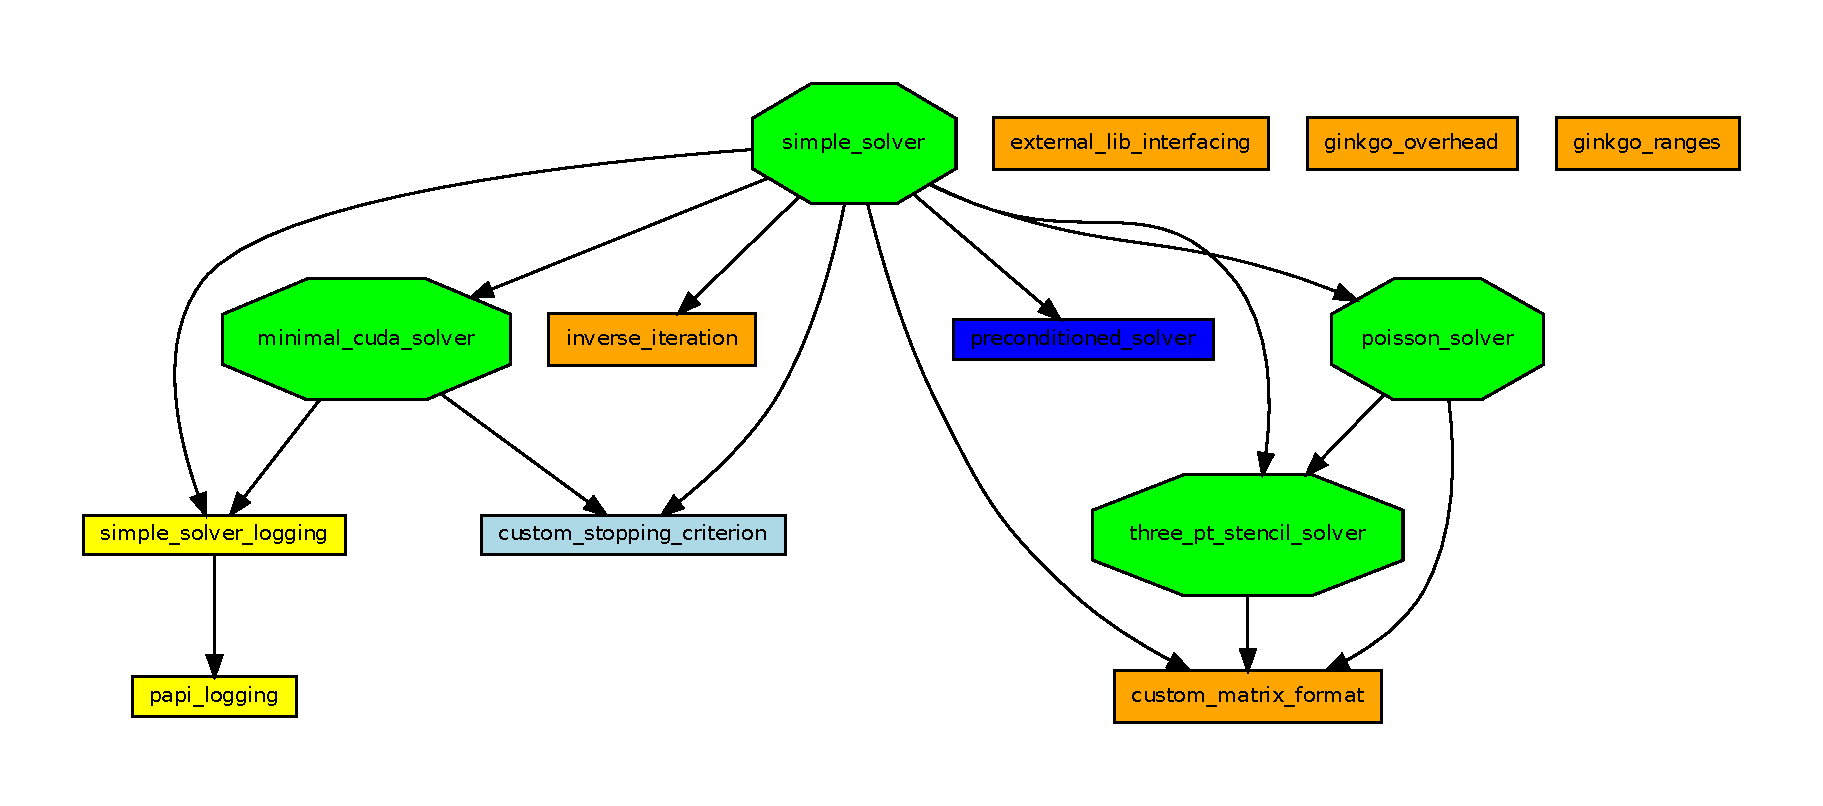
\includegraphics[width=\textwidth,height=\textheight/2,keepaspectratio=true]{dot_inline_dotgraph_1}}
\end{DoxyImageNoCaption}


{\bfseries Legend\+:}~\newline
 
\begin{DoxyImageNoCaption}
  \mbox{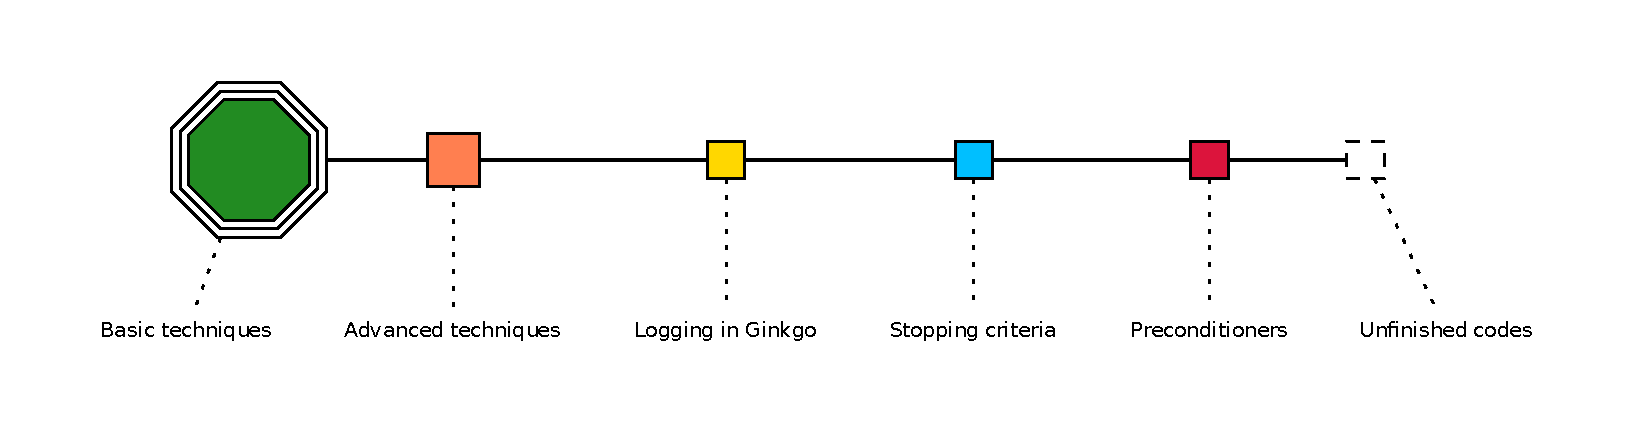
\includegraphics[width=\textwidth,height=\textheight/2,keepaspectratio=true]{dot_inline_dotgraph_2}}
\end{DoxyImageNoCaption}


\label{_list}%
 \subsubsection*{Example programs }

\tabulinesep=1mm
\begin{longtabu} spread 0pt [c]{*{2}{|X[-1]}|}
\hline
\hyperlink{simple_solver}{The simple-\/solver program} &A minimal CG solver in Ginkgo, which reads a matrix from a file. 

\\\cline{1-2}
\hyperlink{minimal_cuda_solver}{The minimal-\/cuda-\/solver program} &A minimal solver on the C\+U\+DA executor than can be run on N\+V\+I\+D\+IA G\+PU\textquotesingle{}s. 

\\\cline{1-2}
\hyperlink{poisson_solver}{The poisson-\/solver program} &Solve an actual physically relevant problem, the poisson problem. The matrix is generated within Ginkgo. 

\\\cline{1-2}
\hyperlink{preconditioned_solver}{The preconditioned-\/solver program} &Using a Jacobi preconditioner to solve a linear system. 

\\\cline{1-2}
\hyperlink{three_pt_stencil_solver}{The three-\/pt-\/stencil-\/solver program} &Using a three point stencil to solve the poisson equation with array views. 

\\\cline{1-2}
\hyperlink{external_lib_interfacing}{The external-\/lib-\/interfacing program} &Using Ginkgo\textquotesingle{}s solver with the external library deal.\+II. 

\\\cline{1-2}
\hyperlink{custom_logger}{The custom-\/logger program} &Creating a custom logger specifically for comparing the recurrent and the real residual norms. 

\\\cline{1-2}
\hyperlink{custom_matrix_format}{The custom-\/matrix-\/format program} &Creating a matrix-\/free stencil solver by using Ginkgo\textquotesingle{}s advanced methods to build your own custom matrix format. 

\\\cline{1-2}
\hyperlink{inverse_iteration}{The inverse-\/iteration program} &Using Ginkgo to compute eigenvalues of a matrix with the inverse iteration method. 

\\\cline{1-2}
\hyperlink{simple_solver_logging}{The simple-\/solver-\/logging program} &Using the logging functionality in Ginkgo to get solver and other information to diagnose and debug your code. 

\\\cline{1-2}
\hyperlink{papi_logging}{The papi-\/logging program} &Using the P\+A\+PI logging library in Ginkgo to get advanced information about your code and its behaviour. 

\\\cline{1-2}
\hyperlink{ginkgo_overhead}{The ginkgo-\/overhead program} &Measuring the overhead of the Ginkgo library. 

\\\cline{1-2}
\hyperlink{custom_stopping_criterion}{The custom-\/stopping-\/criterion program} &Creating a custom stopping criterion for the iterative solution process. 

\\\cline{1-2}
\hyperlink{ginkgo_ranges}{The ginkgo-\/ranges program} &Using the ranges concept to factorize a matrix with the LU factorization. 

\\\cline{1-2}
\end{longtabu}


\label{_topic}%
 \subsubsection*{Example programs grouped by topics}

\paragraph*{{\bfseries Basic techniques}}

\tabulinesep=1mm
\begin{longtabu} spread 0pt [c]{*{2}{|X[-1]}|}
\hline
Solving a simple linear system with choice of executors.  &\hyperlink{simple_solver}{The simple-\/solver program}  

\\\cline{1-2}
Using the C\+U\+DA executor  &\hyperlink{minimal_cuda_solver}{The minimal-\/cuda-\/solver program}  

\\\cline{1-2}
Using preconditioners  &\hyperlink{preconditioned_solver}{The preconditioned-\/solver program}  

\\\cline{1-2}
Solving a physically relevant problem  &\hyperlink{poisson_solver}{The poisson-\/solver program}, \hyperlink{three_pt_stencil_solver}{The three-\/pt-\/stencil-\/solver program}, \hyperlink{custom_matrix_format}{The custom-\/matrix-\/format program}  

\\\cline{1-2}
Reading in a matrix and right hand side from a file.  &\hyperlink{simple_solver}{The simple-\/solver program}, \hyperlink{minimal_cuda_solver}{The minimal-\/cuda-\/solver program}, \hyperlink{preconditioned_solver}{The preconditioned-\/solver program}, \hyperlink{inverse_iteration}{The inverse-\/iteration program}, \hyperlink{simple_solver_logging}{The simple-\/solver-\/logging program}, \hyperlink{papi_logging}{The papi-\/logging program}, \hyperlink{custom_stopping_criterion}{The custom-\/stopping-\/criterion program}, \hyperlink{custom_logger}{The custom-\/logger program}  

\\\cline{1-2}
\end{longtabu}


\paragraph*{{\bfseries Advanced techniques}}

\tabulinesep=1mm
\begin{longtabu} spread 0pt [c]{*{2}{|X[-1]}|}
\hline
Using Ginkgo with external libraries.  &\hyperlink{external_lib_interfacing}{The external-\/lib-\/interfacing program}  

\\\cline{1-2}
Customizing Ginkgo  &\hyperlink{custom_logger}{The custom-\/logger program}, \hyperlink{custom_stopping_criterion}{The custom-\/stopping-\/criterion program}, \hyperlink{custom_matrix_format}{The custom-\/matrix-\/format program}  

\\\cline{1-2}
Writing your own matrix format  &\hyperlink{custom_matrix_format}{The custom-\/matrix-\/format program}  

\\\cline{1-2}
Using Ginkgo to construct more complex linear algebra routines.  &\hyperlink{inverse_iteration}{The inverse-\/iteration program}  

\\\cline{1-2}
Logging within Ginkgo.  &\hyperlink{simple_solver_logging}{The simple-\/solver-\/logging program}, \hyperlink{papi_logging}{The papi-\/logging program}, \hyperlink{custom_logger}{The custom-\/logger program}  

\\\cline{1-2}
Constructing your own stopping criterion.  &\hyperlink{custom_stopping_criterion}{The custom-\/stopping-\/criterion program}  

\\\cline{1-2}
Using ranges in Ginkgo.  &\hyperlink{ginkgo_ranges}{The ginkgo-\/ranges program}   \\\cline{1-2}
\end{longtabu}

\chapter{The custom-\/matrix-\/format program}
\label{custom_matrix_format}
\Hypertarget{custom_matrix_format}
The custom matrix format example..

This example depends on simple-\/solver, poisson-\/solver, three-\/pt-\/stencil-\/solver, .

 \label{_Intro}%
 \label{_Introduction}%
\doxysection*{Introduction}

This example solves a 1D Poisson equation\+:

$ u : [0, 1] \rightarrow R\\ u\text{'}\text{'} = f\\ u(0) = u0\\ u(1) = u1 $

using a finite difference method on an equidistant grid with {\ttfamily K} discretization points ({\ttfamily K} can be controlled with a command line parameter). The discretization is done via the second order Taylor polynomial\+:

$ u(x + h) = u(x) - u\text{'}(x)h + 1/2 u\text{'}\text{'}(x)h^2 + O(h^3)\\ u(x - h) = u(x) + u\text{'}(x)h + 1/2 u\text{'}\text{'}(x)h^2 + O(h^3) / +\\ ---------------------- \\ -u(x - h) + 2u(x) + -u(x + h) = -f(x)h^2 + O(h^3) $

For an equidistant grid with K \char`\"{}inner\char`\"{} discretization points $x1, ..., xk, $and step size $ h = 1 / (K + 1)$, the formula produces a system of linear equations

$ 2u_1 - u_2 = -f_1 h^2 + u0\\ -u_(k-1) + 2u_k - u_(k+1) = -f_k h^2, k = 2, ..., K - 1\\ -u_(K-1) + 2u_K = -f_K h^2 + u1\\ $

which is then solved using Ginkgo\textquotesingle{}s implementation of the CG method preconditioned with block-\/\+Jacobi. It is also possible to specify on which executor Ginkgo will solve the system via the command line. The function $`f` $is set to $`f(x) = 6x`$ (making the solution $`u(x) = x^3`$), but that can be changed in the {\ttfamily main} function.

The intention of this example is to show how a custom linear operator can be created and integrated into Ginkgo to achieve performance benefits.

\label{_Abouttheexample}%
\doxysubsubsection*{About the example }

\label{_CommProg}%
 \doxysection*{The commented program}


\begin{DoxyCode}{0}
\DoxyCodeLine{\textcolor{preprocessor}{\#include <iostream>}}
\DoxyCodeLine{\textcolor{preprocessor}{\#include <map>}}
\DoxyCodeLine{\textcolor{preprocessor}{\#include <string>}}
\DoxyCodeLine{}
\DoxyCodeLine{}
\DoxyCodeLine{\textcolor{preprocessor}{\#include <omp.h>}}
\DoxyCodeLine{\textcolor{preprocessor}{\#include <ginkgo/ginkgo.hpp>}}
\end{DoxyCode}


A C\+U\+DA kernel implementing the stencil, which will be used if running on the C\+U\+DA executor. Unfortunately, N\+V\+CC has serious problems interpreting some parts of Ginkgo\textquotesingle{}s code, so the kernel has to be compiled separately.


\begin{DoxyCode}{0}
\DoxyCodeLine{\textcolor{keyword}{template} <\textcolor{keyword}{typename} ValueType>}
\DoxyCodeLine{\textcolor{keywordtype}{void} stencil\_kernel(std::size\_t size, \textcolor{keyword}{const} ValueType *coefs,}
\DoxyCodeLine{                    \textcolor{keyword}{const} ValueType *b, ValueType *x);}
\end{DoxyCode}


A stencil matrix class representing the 3pt stencil linear operator. We include the \mbox{\hyperlink{classgko_1_1EnableLinOp}{gko\+::\+Enable\+Lin\+Op}} mixin which implements the entire Lin\+Op interface, except the two apply\+\_\+impl methods, which get called inside the default implementation of apply (after argument verification) to perform the actual application of the linear operator. In addition, it includes the implementation of the entire Polymorphic\+Object interface.

It also includes the \mbox{\hyperlink{classgko_1_1EnableCreateMethod}{gko\+::\+Enable\+Create\+Method}} mixin which provides a default implementation of the static create method. This method will forward all its arguments to the constructor to create the object, and return an std\+::unique\+\_\+ptr to the created object.


\begin{DoxyCode}{0}
\DoxyCodeLine{\textcolor{keyword}{template} <\textcolor{keyword}{typename} ValueType>}
\DoxyCodeLine{\textcolor{keyword}{class }StencilMatrix : \textcolor{keyword}{public} \mbox{\hyperlink{classgko_1_1EnableLinOp}{gko::EnableLinOp}}<StencilMatrix<ValueType>>,}
\DoxyCodeLine{                      \textcolor{keyword}{public} \mbox{\hyperlink{classgko_1_1EnableCreateMethod}{gko::EnableCreateMethod}}<StencilMatrix<ValueType>> \{}
\DoxyCodeLine{\textcolor{keyword}{public}:}
\end{DoxyCode}


This constructor will be called by the create method. Here we initialize the coefficients of the stencil.


\begin{DoxyCode}{0}
\DoxyCodeLine{    StencilMatrix(std::shared\_ptr<const gko::Executor> exec,}
\DoxyCodeLine{                  \mbox{\hyperlink{namespacegko_a6e5c95df0ae4e47aab2f604a22d98ee7}{gko::size\_type}} size = 0, ValueType left = -\/1.0,}
\DoxyCodeLine{                  ValueType center = 2.0, ValueType right = -\/1.0)}
\DoxyCodeLine{        : \mbox{\hyperlink{namespacegko}{gko}}::EnableLinOp<StencilMatrix>(exec, \mbox{\hyperlink{namespacegko}{gko}}::dim<2>\{size\}),}
\DoxyCodeLine{          coefficients(exec, \{left, center, right\})}
\DoxyCodeLine{    \{\}}
\DoxyCodeLine{}
\DoxyCodeLine{\textcolor{keyword}{protected}:}
\DoxyCodeLine{    \textcolor{keyword}{using} vec = \mbox{\hyperlink{classgko_1_1matrix_1_1Dense}{gko::matrix::Dense<ValueType>}};}
\DoxyCodeLine{    \textcolor{keyword}{using} coef\_type = \mbox{\hyperlink{classgko_1_1Array}{gko::Array<ValueType>}};}
\end{DoxyCode}


Here we implement the application of the linear operator, x = A $\ast$ b. apply\+\_\+impl will be called by the apply method, after the arguments have been moved to the correct executor and the operators checked for conforming sizes.

For simplicity, we assume that there is always only one right hand side and the stride of consecutive elements in the vectors is 1 (both of these are always true in this example).


\begin{DoxyCode}{0}
\DoxyCodeLine{\textcolor{keywordtype}{void} apply\_impl(\textcolor{keyword}{const} \mbox{\hyperlink{classgko_1_1LinOp}{gko::LinOp}} *b, \mbox{\hyperlink{classgko_1_1LinOp}{gko::LinOp}} *x)\textcolor{keyword}{ const override}}
\DoxyCodeLine{\textcolor{keyword}{}\{}
\end{DoxyCode}


we only implement the operator for dense R\+HS. \mbox{\hyperlink{namespacegko_a73ce7e87aec389b5210630bb617b4baa}{gko\+::as}} will throw an exception if its argument is not Dense.


\begin{DoxyCode}{0}
\DoxyCodeLine{\textcolor{keyword}{auto} dense\_b = gko::as<vec>(b);}
\DoxyCodeLine{\textcolor{keyword}{auto} dense\_x = gko::as<vec>(x);}
\end{DoxyCode}


we need separate implementations depending on the executor, so we create an operation which maps the call to the correct implementation


\begin{DoxyCode}{0}
\DoxyCodeLine{\textcolor{keyword}{struct }stencil\_operation : \mbox{\hyperlink{classgko_1_1Operation}{gko::Operation}} \{}
\DoxyCodeLine{    stencil\_operation(\textcolor{keyword}{const} coef\_type \&coefficients, \textcolor{keyword}{const} vec *b,}
\DoxyCodeLine{                      vec *x)}
\DoxyCodeLine{        : coefficients\{coefficients\}, b\{b\}, x\{x\}}
\DoxyCodeLine{    \{\}}
\end{DoxyCode}


Open\+MP implementation


\begin{DoxyCode}{0}
\DoxyCodeLine{            \textcolor{keywordtype}{void} run(std::shared\_ptr<const gko::OmpExecutor>)\textcolor{keyword}{ const override}}
\DoxyCodeLine{\textcolor{keyword}{            }\{}
\DoxyCodeLine{                \textcolor{keyword}{auto} b\_values = b-\/>get\_const\_values();}
\DoxyCodeLine{                \textcolor{keyword}{auto} x\_values = x-\/>get\_values();}
\DoxyCodeLine{\textcolor{preprocessor}{\#pragma omp parallel for}}
\DoxyCodeLine{                \textcolor{keywordflow}{for} (std::size\_t i = 0; i < x-\/>\mbox{\hyperlink{classgko_1_1LinOp_a31b3c003388eb0b95393154f68c2b98d}{get\_size}}()[0]; ++i) \{}
\DoxyCodeLine{                    \textcolor{keyword}{auto} coefs = coefficients.get\_const\_data();}
\DoxyCodeLine{                    \textcolor{keyword}{auto} result = coefs[1] * b\_values[i];}
\DoxyCodeLine{                    \textcolor{keywordflow}{if} (i > 0) \{}
\DoxyCodeLine{                        result += coefs[0] * b\_values[i -\/ 1];}
\DoxyCodeLine{                    \}}
\DoxyCodeLine{                    \textcolor{keywordflow}{if} (i < x-\/>get\_size()[0] -\/ 1) \{}
\DoxyCodeLine{                        result += coefs[2] * b\_values[i + 1];}
\DoxyCodeLine{                    \}}
\DoxyCodeLine{                    x\_values[i] = result;}
\DoxyCodeLine{                \}}
\DoxyCodeLine{            \}}
\end{DoxyCode}


C\+U\+DA implementation


\begin{DoxyCode}{0}
\DoxyCodeLine{\textcolor{keywordtype}{void} run(std::shared\_ptr<const gko::CudaExecutor>)\textcolor{keyword}{ const override}}
\DoxyCodeLine{\textcolor{keyword}{}\{}
\DoxyCodeLine{    stencil\_kernel(x-\/>\mbox{\hyperlink{classgko_1_1LinOp_a31b3c003388eb0b95393154f68c2b98d}{get\_size}}()[0], coefficients.get\_const\_data(),}
\DoxyCodeLine{                   b-\/>get\_const\_values(), x-\/>get\_values());}
\DoxyCodeLine{\}}
\end{DoxyCode}


We do not provide an implementation for reference executor. If not provided, Ginkgo will use the implementation for the Open\+MP executor when calling it in the reference executor.


\begin{DoxyCode}{0}
\DoxyCodeLine{        \textcolor{keyword}{const} coef\_type \&coefficients;}
\DoxyCodeLine{        \textcolor{keyword}{const} vec *b;}
\DoxyCodeLine{        vec *x;}
\DoxyCodeLine{    \};}
\DoxyCodeLine{    this-\/>get\_executor()-\/>run(}
\DoxyCodeLine{        stencil\_operation(coefficients, dense\_b, dense\_x));}
\DoxyCodeLine{\}}
\end{DoxyCode}


There is also a version of the apply function which does the operation x = alpha $\ast$ A $\ast$ b + beta $\ast$ x. This function is commonly used and can often be better optimized than implementing it using x = A $\ast$ b. However, for simplicity, we will implement it exactly like that in this example.


\begin{DoxyCode}{0}
\DoxyCodeLine{    \textcolor{keywordtype}{void} apply\_impl(\textcolor{keyword}{const} \mbox{\hyperlink{classgko_1_1LinOp}{gko::LinOp}} *alpha, \textcolor{keyword}{const} \mbox{\hyperlink{classgko_1_1LinOp}{gko::LinOp}} *b,}
\DoxyCodeLine{                    \textcolor{keyword}{const} \mbox{\hyperlink{classgko_1_1LinOp}{gko::LinOp}} *beta, \mbox{\hyperlink{classgko_1_1LinOp}{gko::LinOp}} *x)\textcolor{keyword}{ const override}}
\DoxyCodeLine{\textcolor{keyword}{    }\{}
\DoxyCodeLine{        \textcolor{keyword}{auto} dense\_b = gko::as<vec>(b);}
\DoxyCodeLine{        \textcolor{keyword}{auto} dense\_x = gko::as<vec>(x);}
\DoxyCodeLine{        \textcolor{keyword}{auto} tmp\_x = dense\_x-\/>clone();}
\DoxyCodeLine{        this-\/>apply\_impl(b, \mbox{\hyperlink{namespacegko_a4edc2273b5627ec552ea423b60493be3}{lend}}(tmp\_x));}
\DoxyCodeLine{        dense\_x-\/>scale(beta);}
\DoxyCodeLine{        dense\_x-\/>add\_scaled(alpha, \mbox{\hyperlink{namespacegko_a4edc2273b5627ec552ea423b60493be3}{lend}}(tmp\_x));}
\DoxyCodeLine{    \}}
\DoxyCodeLine{}
\DoxyCodeLine{\textcolor{keyword}{private}:}
\DoxyCodeLine{    coef\_type coefficients;}
\DoxyCodeLine{\};}
\end{DoxyCode}


Creates a stencil matrix in C\+SR format for the given number of discretization points.


\begin{DoxyCode}{0}
\DoxyCodeLine{\textcolor{keyword}{template} <\textcolor{keyword}{typename} ValueType, \textcolor{keyword}{typename} IndexType>}
\DoxyCodeLine{\textcolor{keywordtype}{void} generate\_stencil\_matrix(\mbox{\hyperlink{classgko_1_1matrix_1_1Csr}{gko::matrix::Csr<ValueType, IndexType>}} *matrix)}
\DoxyCodeLine{\{}
\DoxyCodeLine{    \textcolor{keyword}{const} \textcolor{keyword}{auto} discretization\_points = matrix-\/>\mbox{\hyperlink{classgko_1_1LinOp_a31b3c003388eb0b95393154f68c2b98d}{get\_size}}()[0];}
\DoxyCodeLine{    \textcolor{keyword}{auto} row\_ptrs = matrix-\/>\mbox{\hyperlink{classgko_1_1matrix_1_1Csr_a068e5158cf282fa977f0a137f8cd7f03}{get\_row\_ptrs}}();}
\DoxyCodeLine{    \textcolor{keyword}{auto} col\_idxs = matrix-\/>\mbox{\hyperlink{classgko_1_1matrix_1_1Csr_a81c6294177a1be4873804c8a85a9fc64}{get\_col\_idxs}}();}
\DoxyCodeLine{    \textcolor{keyword}{auto} values = matrix-\/>\mbox{\hyperlink{classgko_1_1matrix_1_1Csr_a929b0a194e6aeb1252b8e6781d162e83}{get\_values}}();}
\DoxyCodeLine{    IndexType pos = 0;}
\DoxyCodeLine{    \textcolor{keyword}{const} ValueType coefs[] = \{-\/1, 2, -\/1\};}
\DoxyCodeLine{    row\_ptrs[0] = pos;}
\DoxyCodeLine{    \textcolor{keywordflow}{for} (\textcolor{keywordtype}{int} i = 0; i < discretization\_points; ++i) \{}
\DoxyCodeLine{        \textcolor{keywordflow}{for} (\textcolor{keyword}{auto} ofs : \{-\/1, 0, 1\}) \{}
\DoxyCodeLine{            \textcolor{keywordflow}{if} (0 <= i + ofs \&\& i + ofs < discretization\_points) \{}
\DoxyCodeLine{                values[pos] = coefs[ofs + 1];}
\DoxyCodeLine{                col\_idxs[pos] = i + ofs;}
\DoxyCodeLine{                ++pos;}
\DoxyCodeLine{            \}}
\DoxyCodeLine{        \}}
\DoxyCodeLine{        row\_ptrs[i + 1] = pos;}
\DoxyCodeLine{    \}}
\DoxyCodeLine{\}}
\end{DoxyCode}


Generates the R\+HS vector given {\ttfamily f} and the boundary conditions.


\begin{DoxyCode}{0}
\DoxyCodeLine{\textcolor{keyword}{template} <\textcolor{keyword}{typename} Closure, \textcolor{keyword}{typename} ValueType>}
\DoxyCodeLine{\textcolor{keywordtype}{void} generate\_rhs(Closure f, ValueType u0, ValueType u1,}
\DoxyCodeLine{                  \mbox{\hyperlink{classgko_1_1matrix_1_1Dense}{gko::matrix::Dense<ValueType>}} *rhs)}
\DoxyCodeLine{\{}
\DoxyCodeLine{    \textcolor{keyword}{const} \textcolor{keyword}{auto} discretization\_points = rhs-\/>\mbox{\hyperlink{classgko_1_1LinOp_a31b3c003388eb0b95393154f68c2b98d}{get\_size}}()[0];}
\DoxyCodeLine{    \textcolor{keyword}{auto} values = rhs-\/>\mbox{\hyperlink{classgko_1_1matrix_1_1Dense_a3bc458e02fab8e4c9f60f70bd4d5a4f9}{get\_values}}();}
\DoxyCodeLine{    \textcolor{keyword}{const} ValueType h = 1.0 / (discretization\_points + 1);}
\DoxyCodeLine{    \textcolor{keywordflow}{for} (\textcolor{keywordtype}{int} i = 0; i < discretization\_points; ++i) \{}
\DoxyCodeLine{        \textcolor{keyword}{const} ValueType xi = ValueType(i + 1) * h;}
\DoxyCodeLine{        values[i] = -\/f(xi) * h * h;}
\DoxyCodeLine{    \}}
\DoxyCodeLine{    values[0] += u0;}
\DoxyCodeLine{    values[discretization\_points -\/ 1] += u1;}
\DoxyCodeLine{\}}
\end{DoxyCode}


Prints the solution {\ttfamily u}.


\begin{DoxyCode}{0}
\DoxyCodeLine{\textcolor{keyword}{template} <\textcolor{keyword}{typename} ValueType>}
\DoxyCodeLine{\textcolor{keywordtype}{void} print\_solution(ValueType u0, ValueType u1,}
\DoxyCodeLine{                    \textcolor{keyword}{const} \mbox{\hyperlink{classgko_1_1matrix_1_1Dense}{gko::matrix::Dense<ValueType>}} *u)}
\DoxyCodeLine{\{}
\DoxyCodeLine{    std::cout << u0 << \textcolor{charliteral}{'\(\backslash\)n'};}
\DoxyCodeLine{    \textcolor{keywordflow}{for} (\textcolor{keywordtype}{int} i = 0; i < u-\/>\mbox{\hyperlink{classgko_1_1LinOp_a31b3c003388eb0b95393154f68c2b98d}{get\_size}}()[0]; ++i) \{}
\DoxyCodeLine{        std::cout << u-\/>\mbox{\hyperlink{classgko_1_1matrix_1_1Dense_ab83c739c1b11abaecc3bfd89506f6c9c}{get\_const\_values}}()[i] << \textcolor{charliteral}{'\(\backslash\)n'};}
\DoxyCodeLine{    \}}
\DoxyCodeLine{    std::cout << u1 << std::endl;}
\DoxyCodeLine{\}}
\end{DoxyCode}


Computes the 1-\/norm of the error given the computed {\ttfamily u} and the correct solution function {\ttfamily correct\+\_\+u}.


\begin{DoxyCode}{0}
\DoxyCodeLine{\textcolor{keyword}{template} <\textcolor{keyword}{typename} Closure, \textcolor{keyword}{typename} ValueType>}
\DoxyCodeLine{\textcolor{keywordtype}{double} calculate\_error(\textcolor{keywordtype}{int} discretization\_points,}
\DoxyCodeLine{                       \textcolor{keyword}{const} \mbox{\hyperlink{classgko_1_1matrix_1_1Dense}{gko::matrix::Dense<ValueType>}} *u,}
\DoxyCodeLine{                       Closure correct\_u)}
\DoxyCodeLine{\{}
\DoxyCodeLine{    \textcolor{keyword}{const} \textcolor{keyword}{auto} h = 1.0 / (discretization\_points + 1);}
\DoxyCodeLine{    \textcolor{keyword}{auto} error = 0.0;}
\DoxyCodeLine{    \textcolor{keywordflow}{for} (\textcolor{keywordtype}{int} i = 0; i < discretization\_points; ++i) \{}
\DoxyCodeLine{        \textcolor{keyword}{using} std::abs;}
\DoxyCodeLine{        \textcolor{keyword}{const} \textcolor{keyword}{auto} xi = (i + 1) * h;}
\DoxyCodeLine{        error +=}
\DoxyCodeLine{            \mbox{\hyperlink{namespacegko_a57797fc0a00fd4b7ff34ca4bfc84bc51}{abs}}(u-\/>\mbox{\hyperlink{classgko_1_1matrix_1_1Dense_ab83c739c1b11abaecc3bfd89506f6c9c}{get\_const\_values}}()[i] -\/ correct\_u(xi)) / \mbox{\hyperlink{namespacegko_a57797fc0a00fd4b7ff34ca4bfc84bc51}{abs}}(correct\_u(xi));}
\DoxyCodeLine{    \}}
\DoxyCodeLine{    \textcolor{keywordflow}{return} error;}
\DoxyCodeLine{\}}
\DoxyCodeLine{}
\DoxyCodeLine{}
\DoxyCodeLine{\textcolor{keywordtype}{int} main(\textcolor{keywordtype}{int} argc, \textcolor{keywordtype}{char} *argv[])}
\DoxyCodeLine{\{}
\end{DoxyCode}


Some shortcuts


\begin{DoxyCode}{0}
\DoxyCodeLine{\textcolor{keyword}{using} ValueType = double;}
\DoxyCodeLine{\textcolor{keyword}{using} IndexType = int;}
\DoxyCodeLine{}
\DoxyCodeLine{\textcolor{keyword}{using} vec = \mbox{\hyperlink{classgko_1_1matrix_1_1Dense}{gko::matrix::Dense<ValueType>}};}
\DoxyCodeLine{\textcolor{keyword}{using} mtx = \mbox{\hyperlink{classgko_1_1matrix_1_1Csr}{gko::matrix::Csr<ValueType, IndexType>}};}
\DoxyCodeLine{\textcolor{keyword}{using} cg = \mbox{\hyperlink{classgko_1_1solver_1_1Cg}{gko::solver::Cg<ValueType>}};}
\DoxyCodeLine{}
\DoxyCodeLine{\textcolor{keywordflow}{if} (argc < 2) \{}
\DoxyCodeLine{    std::cerr << \textcolor{stringliteral}{"Usage: "} << argv[0] << \textcolor{stringliteral}{" DISCRETIZATION\_POINTS [executor]"}}
\DoxyCodeLine{              << std::endl;}
\DoxyCodeLine{    std::exit(-\/1);}
\DoxyCodeLine{\}}
\end{DoxyCode}


Get number of discretization points


\begin{DoxyCode}{0}
\DoxyCodeLine{\textcolor{keyword}{const} \textcolor{keywordtype}{unsigned} \textcolor{keywordtype}{int} discretization\_points =}
\DoxyCodeLine{    argc >= 2 ? std::atoi(argv[1]) : 100u;}
\DoxyCodeLine{\textcolor{keyword}{const} \textcolor{keyword}{auto} executor\_string = argc >= 3 ? argv[2] : \textcolor{stringliteral}{"reference"};}
\end{DoxyCode}


Figure out where to run the code


\begin{DoxyCode}{0}
\DoxyCodeLine{\textcolor{keyword}{const} \textcolor{keyword}{auto} omp = \mbox{\hyperlink{classgko_1_1OmpExecutor_a33ca05fdd0fc928ee262fc9425304874}{gko::OmpExecutor::create}}();}
\DoxyCodeLine{std::map<std::string, std::shared\_ptr<gko::Executor>> exec\_map\{}
\DoxyCodeLine{    \{\textcolor{stringliteral}{"omp"}, omp\},}
\DoxyCodeLine{    \{\textcolor{stringliteral}{"cuda"}, \mbox{\hyperlink{classgko_1_1CudaExecutor_aa577135e082f9be20617e9d66209ca25}{gko::CudaExecutor::create}}(0, omp, \textcolor{keyword}{true})\},}
\DoxyCodeLine{    \{\textcolor{stringliteral}{"hip"}, \mbox{\hyperlink{classgko_1_1HipExecutor_abee0dc3dfc064c9edbdc02c2b3b11264}{gko::HipExecutor::create}}(0, omp, \textcolor{keyword}{true})\},}
\DoxyCodeLine{    \{\textcolor{stringliteral}{"reference"}, gko::ReferenceExecutor::create()\}\};}
\end{DoxyCode}


executor where Ginkgo will perform the computation


\begin{DoxyCode}{0}
\DoxyCodeLine{\textcolor{keyword}{const} \textcolor{keyword}{auto} exec = exec\_map.at(executor\_string);  \textcolor{comment}{// throws if not valid}}
\end{DoxyCode}


executor used by the application


\begin{DoxyCode}{0}
\DoxyCodeLine{\textcolor{keyword}{const} \textcolor{keyword}{auto} app\_exec = exec\_map[\textcolor{stringliteral}{"omp"}];}
\end{DoxyCode}


problem\+:


\begin{DoxyCode}{0}
\DoxyCodeLine{\textcolor{keyword}{auto} correct\_u = [](ValueType x) \{ \textcolor{keywordflow}{return} x * x * x; \};}
\DoxyCodeLine{\textcolor{keyword}{auto} f = [](ValueType x) \{ \textcolor{keywordflow}{return} ValueType(6) * x; \};}
\DoxyCodeLine{\textcolor{keyword}{auto} u0 = correct\_u(0);}
\DoxyCodeLine{\textcolor{keyword}{auto} u1 = correct\_u(1);}
\end{DoxyCode}


initialize vectors


\begin{DoxyCode}{0}
\DoxyCodeLine{\textcolor{keyword}{auto} rhs = vec::create(app\_exec, \mbox{\hyperlink{structgko_1_1dim}{gko::dim<2>}}(discretization\_points, 1));}
\DoxyCodeLine{generate\_rhs(f, u0, u1, \mbox{\hyperlink{namespacegko_a4edc2273b5627ec552ea423b60493be3}{lend}}(rhs));}
\DoxyCodeLine{\textcolor{keyword}{auto} u = vec::create(app\_exec, \mbox{\hyperlink{structgko_1_1dim}{gko::dim<2>}}(discretization\_points, 1));}
\DoxyCodeLine{\textcolor{keywordflow}{for} (\textcolor{keywordtype}{int} i = 0; i < u-\/>\mbox{\hyperlink{classgko_1_1LinOp_a31b3c003388eb0b95393154f68c2b98d}{get\_size}}()[0]; ++i) \{}
\DoxyCodeLine{    u-\/>\mbox{\hyperlink{classgko_1_1matrix_1_1Dense_a3bc458e02fab8e4c9f60f70bd4d5a4f9}{get\_values}}()[i] = 0.0;}
\DoxyCodeLine{\}}
\DoxyCodeLine{}
\DoxyCodeLine{\textcolor{keyword}{const} ValueType reduction\_factor = 1e-\/7;}
\end{DoxyCode}


Generate solver and solve the system


\begin{DoxyCode}{0}
\DoxyCodeLine{cg::build()}
\DoxyCodeLine{    .with\_criteria(gko::stop::Iteration::build()}
\DoxyCodeLine{                       .with\_max\_iters(discretization\_points)}
\DoxyCodeLine{                       .on(exec),}
\DoxyCodeLine{                   \mbox{\hyperlink{classgko_1_1stop_1_1ResidualNormReduction}{gko::stop::ResidualNormReduction<ValueType>::build}}()}
\DoxyCodeLine{                       .with\_reduction\_factor(reduction\_factor)}
\DoxyCodeLine{                       .on(exec))}
\DoxyCodeLine{    .on(exec)}
\end{DoxyCode}


notice how our custom Stencil\+Matrix can be used in the same way as any built-\/in type


\begin{DoxyCode}{0}
\DoxyCodeLine{        -\/>generate(StencilMatrix<ValueType>::create(exec, discretization\_points,}
\DoxyCodeLine{                                                    -\/1, 2, -\/1))}
\DoxyCodeLine{        -\/>apply(\mbox{\hyperlink{namespacegko_a4edc2273b5627ec552ea423b60493be3}{lend}}(rhs), \mbox{\hyperlink{namespacegko_a4edc2273b5627ec552ea423b60493be3}{lend}}(u));}
\DoxyCodeLine{}
\DoxyCodeLine{    print\_solution(u0, u1, \mbox{\hyperlink{namespacegko_a4edc2273b5627ec552ea423b60493be3}{lend}}(u));}
\DoxyCodeLine{    std::cout << \textcolor{stringliteral}{"The average relative error is "}}
\DoxyCodeLine{              << calculate\_error(discretization\_points, \mbox{\hyperlink{namespacegko_a4edc2273b5627ec552ea423b60493be3}{lend}}(u), correct\_u) /}
\DoxyCodeLine{                     discretization\_points}
\DoxyCodeLine{              << std::endl;}
\DoxyCodeLine{\}}
\end{DoxyCode}
 \label{_Results}%
\doxysection*{Results}

\label{_Commentsaboutprogramminganddebugging}%
\doxysubsubsection*{Comments about programming and debugging }

\label{_PlainProg}%
 \doxysection*{The plain program}


\begin{DoxyCodeInclude}{0}
\DoxyCodeLine{\textcolor{comment}{/*******************************<GINKGO LICENSE>******************************}}
\DoxyCodeLine{\textcolor{comment}{Copyright (c) 2017-\/2020, the Ginkgo authors}}
\DoxyCodeLine{\textcolor{comment}{All rights reserved.}}
\DoxyCodeLine{\textcolor{comment}{}}
\DoxyCodeLine{\textcolor{comment}{Redistribution and use in source and binary forms, with or without}}
\DoxyCodeLine{\textcolor{comment}{modification, are permitted provided that the following conditions}}
\DoxyCodeLine{\textcolor{comment}{are met:}}
\DoxyCodeLine{\textcolor{comment}{}}
\DoxyCodeLine{\textcolor{comment}{1. Redistributions of source code must retain the above copyright}}
\DoxyCodeLine{\textcolor{comment}{notice, this list of conditions and the following disclaimer.}}
\DoxyCodeLine{\textcolor{comment}{}}
\DoxyCodeLine{\textcolor{comment}{2. Redistributions in binary form must reproduce the above copyright}}
\DoxyCodeLine{\textcolor{comment}{notice, this list of conditions and the following disclaimer in the}}
\DoxyCodeLine{\textcolor{comment}{documentation and/or other materials provided with the distribution.}}
\DoxyCodeLine{\textcolor{comment}{}}
\DoxyCodeLine{\textcolor{comment}{3. Neither the name of the copyright holder nor the names of its}}
\DoxyCodeLine{\textcolor{comment}{contributors may be used to endorse or promote products derived from}}
\DoxyCodeLine{\textcolor{comment}{this software without specific prior written permission.}}
\DoxyCodeLine{\textcolor{comment}{}}
\DoxyCodeLine{\textcolor{comment}{THIS SOFTWARE IS PROVIDED BY THE COPYRIGHT HOLDERS AND CONTRIBUTORS "AS}}
\DoxyCodeLine{\textcolor{comment}{IS" AND ANY EXPRESS OR IMPLIED WARRANTIES, INCLUDING, BUT NOT LIMITED}}
\DoxyCodeLine{\textcolor{comment}{TO, THE IMPLIED WARRANTIES OF MERCHANTABILITY AND FITNESS FOR A}}
\DoxyCodeLine{\textcolor{comment}{PARTICULAR PURPOSE ARE DISCLAIMED. IN NO EVENT SHALL THE COPYRIGHT}}
\DoxyCodeLine{\textcolor{comment}{HOLDER OR CONTRIBUTORS BE LIABLE FOR ANY DIRECT, INDIRECT, INCIDENTAL,}}
\DoxyCodeLine{\textcolor{comment}{SPECIAL, EXEMPLARY, OR CONSEQUENTIAL DAMAGES (INCLUDING, BUT NOT}}
\DoxyCodeLine{\textcolor{comment}{LIMITED TO, PROCUREMENT OF SUBSTITUTE GOODS OR SERVICES; LOSS OF USE,}}
\DoxyCodeLine{\textcolor{comment}{DATA, OR PROFITS; OR BUSINESS INTERRUPTION) HOWEVER CAUSED AND ON ANY}}
\DoxyCodeLine{\textcolor{comment}{THEORY OF LIABILITY, WHETHER IN CONTRACT, STRICT LIABILITY, OR TORT}}
\DoxyCodeLine{\textcolor{comment}{(INCLUDING NEGLIGENCE OR OTHERWISE) ARISING IN ANY WAY OUT OF THE USE}}
\DoxyCodeLine{\textcolor{comment}{OF THIS SOFTWARE, EVEN IF ADVISED OF THE POSSIBILITY OF SUCH DAMAGE.}}
\DoxyCodeLine{\textcolor{comment}{******************************<GINKGO LICENSE>*******************************/}}
\DoxyCodeLine{}
\DoxyCodeLine{\textcolor{preprocessor}{\#include <iostream>}}
\DoxyCodeLine{\textcolor{preprocessor}{\#include <map>}}
\DoxyCodeLine{\textcolor{preprocessor}{\#include <string>}}
\DoxyCodeLine{}
\DoxyCodeLine{}
\DoxyCodeLine{\textcolor{preprocessor}{\#include <omp.h>}}
\DoxyCodeLine{\textcolor{preprocessor}{\#include <ginkgo/ginkgo.hpp>}}
\DoxyCodeLine{}
\DoxyCodeLine{}
\DoxyCodeLine{\textcolor{keyword}{template} <\textcolor{keyword}{typename} ValueType>}
\DoxyCodeLine{\textcolor{keywordtype}{void} stencil\_kernel(std::size\_t size, \textcolor{keyword}{const} ValueType *coefs,}
\DoxyCodeLine{                    \textcolor{keyword}{const} ValueType *b, ValueType *x);}
\DoxyCodeLine{}
\DoxyCodeLine{}
\DoxyCodeLine{\textcolor{keyword}{template} <\textcolor{keyword}{typename} ValueType>}
\DoxyCodeLine{\textcolor{keyword}{class }StencilMatrix : \textcolor{keyword}{public} \mbox{\hyperlink{classgko_1_1EnableLinOp}{gko::EnableLinOp}}<StencilMatrix<ValueType>>,}
\DoxyCodeLine{                      \textcolor{keyword}{public} \mbox{\hyperlink{classgko_1_1EnableCreateMethod}{gko::EnableCreateMethod}}<StencilMatrix<ValueType>> \{}
\DoxyCodeLine{\textcolor{keyword}{public}:}
\DoxyCodeLine{    StencilMatrix(std::shared\_ptr<const gko::Executor> exec,}
\DoxyCodeLine{                  \mbox{\hyperlink{namespacegko_a6e5c95df0ae4e47aab2f604a22d98ee7}{gko::size\_type}} size = 0, ValueType left = -\/1.0,}
\DoxyCodeLine{                  ValueType center = 2.0, ValueType right = -\/1.0)}
\DoxyCodeLine{        : \mbox{\hyperlink{namespacegko}{gko}}::EnableLinOp<StencilMatrix>(exec, \mbox{\hyperlink{namespacegko}{gko}}::dim<2>\{size\}),}
\DoxyCodeLine{          coefficients(exec, \{left, center, right\})}
\DoxyCodeLine{    \{\}}
\DoxyCodeLine{}
\DoxyCodeLine{\textcolor{keyword}{protected}:}
\DoxyCodeLine{    \textcolor{keyword}{using} vec = \mbox{\hyperlink{classgko_1_1matrix_1_1Dense}{gko::matrix::Dense<ValueType>}};}
\DoxyCodeLine{    \textcolor{keyword}{using} coef\_type = \mbox{\hyperlink{classgko_1_1Array}{gko::Array<ValueType>}};}
\DoxyCodeLine{}
\DoxyCodeLine{    \textcolor{keywordtype}{void} apply\_impl(\textcolor{keyword}{const} \mbox{\hyperlink{classgko_1_1LinOp}{gko::LinOp}} *b, \mbox{\hyperlink{classgko_1_1LinOp}{gko::LinOp}} *x)\textcolor{keyword}{ const override}}
\DoxyCodeLine{\textcolor{keyword}{    }\{}
\DoxyCodeLine{        \textcolor{keyword}{auto} dense\_b = gko::as<vec>(b);}
\DoxyCodeLine{        \textcolor{keyword}{auto} dense\_x = gko::as<vec>(x);}
\DoxyCodeLine{}
\DoxyCodeLine{        \textcolor{keyword}{struct }stencil\_operation : \mbox{\hyperlink{classgko_1_1Operation}{gko::Operation}} \{}
\DoxyCodeLine{            stencil\_operation(\textcolor{keyword}{const} coef\_type \&coefficients, \textcolor{keyword}{const} vec *b,}
\DoxyCodeLine{                              vec *x)}
\DoxyCodeLine{                : coefficients\{coefficients\}, b\{b\}, x\{x\}}
\DoxyCodeLine{            \{\}}
\DoxyCodeLine{}
\DoxyCodeLine{            \textcolor{keywordtype}{void} run(std::shared\_ptr<const gko::OmpExecutor>)\textcolor{keyword}{ const override}}
\DoxyCodeLine{\textcolor{keyword}{            }\{}
\DoxyCodeLine{                \textcolor{keyword}{auto} b\_values = b-\/>get\_const\_values();}
\DoxyCodeLine{                \textcolor{keyword}{auto} x\_values = x-\/>get\_values();}
\DoxyCodeLine{\textcolor{preprocessor}{\#pragma omp parallel for}}
\DoxyCodeLine{                \textcolor{keywordflow}{for} (std::size\_t i = 0; i < x-\/>\mbox{\hyperlink{classgko_1_1LinOp_a31b3c003388eb0b95393154f68c2b98d}{get\_size}}()[0]; ++i) \{}
\DoxyCodeLine{                    \textcolor{keyword}{auto} coefs = coefficients.get\_const\_data();}
\DoxyCodeLine{                    \textcolor{keyword}{auto} result = coefs[1] * b\_values[i];}
\DoxyCodeLine{                    \textcolor{keywordflow}{if} (i > 0) \{}
\DoxyCodeLine{                        result += coefs[0] * b\_values[i -\/ 1];}
\DoxyCodeLine{                    \}}
\DoxyCodeLine{                    \textcolor{keywordflow}{if} (i < x-\/>get\_size()[0] -\/ 1) \{}
\DoxyCodeLine{                        result += coefs[2] * b\_values[i + 1];}
\DoxyCodeLine{                    \}}
\DoxyCodeLine{                    x\_values[i] = result;}
\DoxyCodeLine{                \}}
\DoxyCodeLine{            \}}
\DoxyCodeLine{}
\DoxyCodeLine{            \textcolor{keywordtype}{void} run(std::shared\_ptr<const gko::CudaExecutor>)\textcolor{keyword}{ const override}}
\DoxyCodeLine{\textcolor{keyword}{            }\{}
\DoxyCodeLine{                stencil\_kernel(x-\/>\mbox{\hyperlink{classgko_1_1LinOp_a31b3c003388eb0b95393154f68c2b98d}{get\_size}}()[0], coefficients.get\_const\_data(),}
\DoxyCodeLine{                               b-\/>get\_const\_values(), x-\/>get\_values());}
\DoxyCodeLine{            \}}
\DoxyCodeLine{}
\DoxyCodeLine{}
\DoxyCodeLine{            \textcolor{keyword}{const} coef\_type \&coefficients;}
\DoxyCodeLine{            \textcolor{keyword}{const} vec *b;}
\DoxyCodeLine{            vec *x;}
\DoxyCodeLine{        \};}
\DoxyCodeLine{        this-\/>get\_executor()-\/>run(}
\DoxyCodeLine{            stencil\_operation(coefficients, dense\_b, dense\_x));}
\DoxyCodeLine{    \}}
\DoxyCodeLine{}
\DoxyCodeLine{    \textcolor{keywordtype}{void} apply\_impl(\textcolor{keyword}{const} \mbox{\hyperlink{classgko_1_1LinOp}{gko::LinOp}} *alpha, \textcolor{keyword}{const} \mbox{\hyperlink{classgko_1_1LinOp}{gko::LinOp}} *b,}
\DoxyCodeLine{                    \textcolor{keyword}{const} \mbox{\hyperlink{classgko_1_1LinOp}{gko::LinOp}} *beta, \mbox{\hyperlink{classgko_1_1LinOp}{gko::LinOp}} *x)\textcolor{keyword}{ const override}}
\DoxyCodeLine{\textcolor{keyword}{    }\{}
\DoxyCodeLine{        \textcolor{keyword}{auto} dense\_b = gko::as<vec>(b);}
\DoxyCodeLine{        \textcolor{keyword}{auto} dense\_x = gko::as<vec>(x);}
\DoxyCodeLine{        \textcolor{keyword}{auto} tmp\_x = dense\_x-\/>clone();}
\DoxyCodeLine{        this-\/>apply\_impl(b, \mbox{\hyperlink{namespacegko_a4edc2273b5627ec552ea423b60493be3}{lend}}(tmp\_x));}
\DoxyCodeLine{        dense\_x-\/>scale(beta);}
\DoxyCodeLine{        dense\_x-\/>add\_scaled(alpha, \mbox{\hyperlink{namespacegko_a4edc2273b5627ec552ea423b60493be3}{lend}}(tmp\_x));}
\DoxyCodeLine{    \}}
\DoxyCodeLine{}
\DoxyCodeLine{\textcolor{keyword}{private}:}
\DoxyCodeLine{    coef\_type coefficients;}
\DoxyCodeLine{\};}
\DoxyCodeLine{}
\DoxyCodeLine{}
\DoxyCodeLine{\textcolor{keyword}{template} <\textcolor{keyword}{typename} ValueType, \textcolor{keyword}{typename} IndexType>}
\DoxyCodeLine{\textcolor{keywordtype}{void} generate\_stencil\_matrix(\mbox{\hyperlink{classgko_1_1matrix_1_1Csr}{gko::matrix::Csr<ValueType, IndexType>}} *matrix)}
\DoxyCodeLine{\{}
\DoxyCodeLine{    \textcolor{keyword}{const} \textcolor{keyword}{auto} discretization\_points = matrix-\/>\mbox{\hyperlink{classgko_1_1LinOp_a31b3c003388eb0b95393154f68c2b98d}{get\_size}}()[0];}
\DoxyCodeLine{    \textcolor{keyword}{auto} row\_ptrs = matrix-\/>\mbox{\hyperlink{classgko_1_1matrix_1_1Csr_a068e5158cf282fa977f0a137f8cd7f03}{get\_row\_ptrs}}();}
\DoxyCodeLine{    \textcolor{keyword}{auto} col\_idxs = matrix-\/>\mbox{\hyperlink{classgko_1_1matrix_1_1Csr_a81c6294177a1be4873804c8a85a9fc64}{get\_col\_idxs}}();}
\DoxyCodeLine{    \textcolor{keyword}{auto} values = matrix-\/>\mbox{\hyperlink{classgko_1_1matrix_1_1Csr_a929b0a194e6aeb1252b8e6781d162e83}{get\_values}}();}
\DoxyCodeLine{    IndexType pos = 0;}
\DoxyCodeLine{    \textcolor{keyword}{const} ValueType coefs[] = \{-\/1, 2, -\/1\};}
\DoxyCodeLine{    row\_ptrs[0] = pos;}
\DoxyCodeLine{    \textcolor{keywordflow}{for} (\textcolor{keywordtype}{int} i = 0; i < discretization\_points; ++i) \{}
\DoxyCodeLine{        \textcolor{keywordflow}{for} (\textcolor{keyword}{auto} ofs : \{-\/1, 0, 1\}) \{}
\DoxyCodeLine{            \textcolor{keywordflow}{if} (0 <= i + ofs \&\& i + ofs < discretization\_points) \{}
\DoxyCodeLine{                values[pos] = coefs[ofs + 1];}
\DoxyCodeLine{                col\_idxs[pos] = i + ofs;}
\DoxyCodeLine{                ++pos;}
\DoxyCodeLine{            \}}
\DoxyCodeLine{        \}}
\DoxyCodeLine{        row\_ptrs[i + 1] = pos;}
\DoxyCodeLine{    \}}
\DoxyCodeLine{\}}
\DoxyCodeLine{}
\DoxyCodeLine{}
\DoxyCodeLine{\textcolor{keyword}{template} <\textcolor{keyword}{typename} Closure, \textcolor{keyword}{typename} ValueType>}
\DoxyCodeLine{\textcolor{keywordtype}{void} generate\_rhs(Closure f, ValueType u0, ValueType u1,}
\DoxyCodeLine{                  \mbox{\hyperlink{classgko_1_1matrix_1_1Dense}{gko::matrix::Dense<ValueType>}} *rhs)}
\DoxyCodeLine{\{}
\DoxyCodeLine{    \textcolor{keyword}{const} \textcolor{keyword}{auto} discretization\_points = rhs-\/>\mbox{\hyperlink{classgko_1_1LinOp_a31b3c003388eb0b95393154f68c2b98d}{get\_size}}()[0];}
\DoxyCodeLine{    \textcolor{keyword}{auto} values = rhs-\/>\mbox{\hyperlink{classgko_1_1matrix_1_1Dense_a3bc458e02fab8e4c9f60f70bd4d5a4f9}{get\_values}}();}
\DoxyCodeLine{    \textcolor{keyword}{const} ValueType h = 1.0 / (discretization\_points + 1);}
\DoxyCodeLine{    \textcolor{keywordflow}{for} (\textcolor{keywordtype}{int} i = 0; i < discretization\_points; ++i) \{}
\DoxyCodeLine{        \textcolor{keyword}{const} ValueType xi = ValueType(i + 1) * h;}
\DoxyCodeLine{        values[i] = -\/f(xi) * h * h;}
\DoxyCodeLine{    \}}
\DoxyCodeLine{    values[0] += u0;}
\DoxyCodeLine{    values[discretization\_points -\/ 1] += u1;}
\DoxyCodeLine{\}}
\DoxyCodeLine{}
\DoxyCodeLine{}
\DoxyCodeLine{\textcolor{keyword}{template} <\textcolor{keyword}{typename} ValueType>}
\DoxyCodeLine{\textcolor{keywordtype}{void} print\_solution(ValueType u0, ValueType u1,}
\DoxyCodeLine{                    \textcolor{keyword}{const} \mbox{\hyperlink{classgko_1_1matrix_1_1Dense}{gko::matrix::Dense<ValueType>}} *u)}
\DoxyCodeLine{\{}
\DoxyCodeLine{    std::cout << u0 << \textcolor{charliteral}{'\(\backslash\)n'};}
\DoxyCodeLine{    \textcolor{keywordflow}{for} (\textcolor{keywordtype}{int} i = 0; i < u-\/>\mbox{\hyperlink{classgko_1_1LinOp_a31b3c003388eb0b95393154f68c2b98d}{get\_size}}()[0]; ++i) \{}
\DoxyCodeLine{        std::cout << u-\/>\mbox{\hyperlink{classgko_1_1matrix_1_1Dense_ab83c739c1b11abaecc3bfd89506f6c9c}{get\_const\_values}}()[i] << \textcolor{charliteral}{'\(\backslash\)n'};}
\DoxyCodeLine{    \}}
\DoxyCodeLine{    std::cout << u1 << std::endl;}
\DoxyCodeLine{\}}
\DoxyCodeLine{}
\DoxyCodeLine{}
\DoxyCodeLine{\textcolor{keyword}{template} <\textcolor{keyword}{typename} Closure, \textcolor{keyword}{typename} ValueType>}
\DoxyCodeLine{\textcolor{keywordtype}{double} calculate\_error(\textcolor{keywordtype}{int} discretization\_points,}
\DoxyCodeLine{                       \textcolor{keyword}{const} \mbox{\hyperlink{classgko_1_1matrix_1_1Dense}{gko::matrix::Dense<ValueType>}} *u,}
\DoxyCodeLine{                       Closure correct\_u)}
\DoxyCodeLine{\{}
\DoxyCodeLine{    \textcolor{keyword}{const} \textcolor{keyword}{auto} h = 1.0 / (discretization\_points + 1);}
\DoxyCodeLine{    \textcolor{keyword}{auto} error = 0.0;}
\DoxyCodeLine{    \textcolor{keywordflow}{for} (\textcolor{keywordtype}{int} i = 0; i < discretization\_points; ++i) \{}
\DoxyCodeLine{        \textcolor{keyword}{using} std::abs;}
\DoxyCodeLine{        \textcolor{keyword}{const} \textcolor{keyword}{auto} xi = (i + 1) * h;}
\DoxyCodeLine{        error +=}
\DoxyCodeLine{            \mbox{\hyperlink{namespacegko_a57797fc0a00fd4b7ff34ca4bfc84bc51}{abs}}(u-\/>\mbox{\hyperlink{classgko_1_1matrix_1_1Dense_ab83c739c1b11abaecc3bfd89506f6c9c}{get\_const\_values}}()[i] -\/ correct\_u(xi)) / \mbox{\hyperlink{namespacegko_a57797fc0a00fd4b7ff34ca4bfc84bc51}{abs}}(correct\_u(xi));}
\DoxyCodeLine{    \}}
\DoxyCodeLine{    \textcolor{keywordflow}{return} error;}
\DoxyCodeLine{\}}
\DoxyCodeLine{}
\DoxyCodeLine{}
\DoxyCodeLine{\textcolor{keywordtype}{int} main(\textcolor{keywordtype}{int} argc, \textcolor{keywordtype}{char} *argv[])}
\DoxyCodeLine{\{}
\DoxyCodeLine{    \textcolor{keyword}{using} ValueType = double;}
\DoxyCodeLine{    \textcolor{keyword}{using} IndexType = int;}
\DoxyCodeLine{}
\DoxyCodeLine{    \textcolor{keyword}{using} vec = \mbox{\hyperlink{classgko_1_1matrix_1_1Dense}{gko::matrix::Dense<ValueType>}};}
\DoxyCodeLine{    \textcolor{keyword}{using} mtx = \mbox{\hyperlink{classgko_1_1matrix_1_1Csr}{gko::matrix::Csr<ValueType, IndexType>}};}
\DoxyCodeLine{    \textcolor{keyword}{using} cg = \mbox{\hyperlink{classgko_1_1solver_1_1Cg}{gko::solver::Cg<ValueType>}};}
\DoxyCodeLine{}
\DoxyCodeLine{    \textcolor{keywordflow}{if} (argc < 2) \{}
\DoxyCodeLine{        std::cerr << \textcolor{stringliteral}{"Usage: "} << argv[0] << \textcolor{stringliteral}{" DISCRETIZATION\_POINTS [executor]"}}
\DoxyCodeLine{                  << std::endl;}
\DoxyCodeLine{        std::exit(-\/1);}
\DoxyCodeLine{    \}}
\DoxyCodeLine{}
\DoxyCodeLine{    \textcolor{keyword}{const} \textcolor{keywordtype}{unsigned} \textcolor{keywordtype}{int} discretization\_points =}
\DoxyCodeLine{        argc >= 2 ? std::atoi(argv[1]) : 100u;}
\DoxyCodeLine{    \textcolor{keyword}{const} \textcolor{keyword}{auto} executor\_string = argc >= 3 ? argv[2] : \textcolor{stringliteral}{"reference"};}
\DoxyCodeLine{}
\DoxyCodeLine{    \textcolor{keyword}{const} \textcolor{keyword}{auto} omp = \mbox{\hyperlink{classgko_1_1OmpExecutor_a33ca05fdd0fc928ee262fc9425304874}{gko::OmpExecutor::create}}();}
\DoxyCodeLine{    std::map<std::string, std::shared\_ptr<gko::Executor>> exec\_map\{}
\DoxyCodeLine{        \{\textcolor{stringliteral}{"omp"}, omp\},}
\DoxyCodeLine{        \{\textcolor{stringliteral}{"cuda"}, \mbox{\hyperlink{classgko_1_1CudaExecutor_aa577135e082f9be20617e9d66209ca25}{gko::CudaExecutor::create}}(0, omp, \textcolor{keyword}{true})\},}
\DoxyCodeLine{        \{\textcolor{stringliteral}{"hip"}, \mbox{\hyperlink{classgko_1_1HipExecutor_abee0dc3dfc064c9edbdc02c2b3b11264}{gko::HipExecutor::create}}(0, omp, \textcolor{keyword}{true})\},}
\DoxyCodeLine{        \{\textcolor{stringliteral}{"reference"}, gko::ReferenceExecutor::create()\}\};}
\DoxyCodeLine{}
\DoxyCodeLine{    \textcolor{keyword}{const} \textcolor{keyword}{auto} exec = exec\_map.at(executor\_string);  \textcolor{comment}{// throws if not valid}}
\DoxyCodeLine{    \textcolor{keyword}{const} \textcolor{keyword}{auto} app\_exec = exec\_map[\textcolor{stringliteral}{"omp"}];}
\DoxyCodeLine{}
\DoxyCodeLine{    \textcolor{keyword}{auto} correct\_u = [](ValueType x) \{ \textcolor{keywordflow}{return} x * x * x; \};}
\DoxyCodeLine{    \textcolor{keyword}{auto} f = [](ValueType x) \{ \textcolor{keywordflow}{return} ValueType(6) * x; \};}
\DoxyCodeLine{    \textcolor{keyword}{auto} u0 = correct\_u(0);}
\DoxyCodeLine{    \textcolor{keyword}{auto} u1 = correct\_u(1);}
\DoxyCodeLine{}
\DoxyCodeLine{    \textcolor{keyword}{auto} rhs = vec::create(app\_exec, \mbox{\hyperlink{structgko_1_1dim}{gko::dim<2>}}(discretization\_points, 1));}
\DoxyCodeLine{    generate\_rhs(f, u0, u1, \mbox{\hyperlink{namespacegko_a4edc2273b5627ec552ea423b60493be3}{lend}}(rhs));}
\DoxyCodeLine{    \textcolor{keyword}{auto} u = vec::create(app\_exec, \mbox{\hyperlink{structgko_1_1dim}{gko::dim<2>}}(discretization\_points, 1));}
\DoxyCodeLine{    \textcolor{keywordflow}{for} (\textcolor{keywordtype}{int} i = 0; i < u-\/>\mbox{\hyperlink{classgko_1_1LinOp_a31b3c003388eb0b95393154f68c2b98d}{get\_size}}()[0]; ++i) \{}
\DoxyCodeLine{        u-\/>\mbox{\hyperlink{classgko_1_1matrix_1_1Dense_a3bc458e02fab8e4c9f60f70bd4d5a4f9}{get\_values}}()[i] = 0.0;}
\DoxyCodeLine{    \}}
\DoxyCodeLine{}
\DoxyCodeLine{    \textcolor{keyword}{const} ValueType reduction\_factor = 1e-\/7;}
\DoxyCodeLine{    cg::build()}
\DoxyCodeLine{        .with\_criteria(gko::stop::Iteration::build()}
\DoxyCodeLine{                           .with\_max\_iters(discretization\_points)}
\DoxyCodeLine{                           .on(exec),}
\DoxyCodeLine{                       \mbox{\hyperlink{classgko_1_1stop_1_1ResidualNormReduction}{gko::stop::ResidualNormReduction<ValueType>::build}}()}
\DoxyCodeLine{                           .with\_reduction\_factor(reduction\_factor)}
\DoxyCodeLine{                           .on(exec))}
\DoxyCodeLine{        .on(exec)}
\DoxyCodeLine{        -\/>generate(StencilMatrix<ValueType>::create(exec, discretization\_points,}
\DoxyCodeLine{                                                    -\/1, 2, -\/1))}
\DoxyCodeLine{        -\/>apply(\mbox{\hyperlink{namespacegko_a4edc2273b5627ec552ea423b60493be3}{lend}}(rhs), \mbox{\hyperlink{namespacegko_a4edc2273b5627ec552ea423b60493be3}{lend}}(u));}
\DoxyCodeLine{}
\DoxyCodeLine{    print\_solution(u0, u1, \mbox{\hyperlink{namespacegko_a4edc2273b5627ec552ea423b60493be3}{lend}}(u));}
\DoxyCodeLine{    std::cout << \textcolor{stringliteral}{"The average relative error is "}}
\DoxyCodeLine{              << calculate\_error(discretization\_points, \mbox{\hyperlink{namespacegko_a4edc2273b5627ec552ea423b60493be3}{lend}}(u), correct\_u) /}
\DoxyCodeLine{                     discretization\_points}
\DoxyCodeLine{              << std::endl;}
\DoxyCodeLine{\}}
\end{DoxyCodeInclude}
 
\chapter{The custom-\/stopping-\/criterion program}
\label{custom_stopping_criterion}
\Hypertarget{custom_stopping_criterion}
The custom stopping criterion creation example..

This example depends on simple-\/solver, minimal-\/cuda-\/solver.

 \label{_Intro}%
 \label{_Introduction}%
\doxysection*{Introduction}

\label{_Abouttheexample}%
\doxysubsubsection*{About the example }

\label{_CommProg}%
 \doxysection*{The commented program}


\begin{DoxyCode}{0}
\DoxyCodeLine{\textcolor{preprocessor}{\#include <ginkgo/ginkgo.hpp>}}
\DoxyCodeLine{}
\DoxyCodeLine{}
\DoxyCodeLine{\textcolor{preprocessor}{\#include <fstream>}}
\DoxyCodeLine{\textcolor{preprocessor}{\#include <iostream>}}
\DoxyCodeLine{\textcolor{preprocessor}{\#include <string>}}
\DoxyCodeLine{\textcolor{preprocessor}{\#include <thread>}}
\DoxyCodeLine{}
\DoxyCodeLine{}
\DoxyCodeLine{/ **}
\DoxyCodeLine{ * The ByInteraction \textcolor{keyword}{class }is a criterion which asks for user input to stop}
\DoxyCodeLine{ * the iteration process. Using \textcolor{keyword}{this} criterion is slightly more complex than the}
\DoxyCodeLine{ * other ones, because it is asynchronous therefore requires the use of threads.}
\DoxyCodeLine{ * /}
\DoxyCodeLine{\textcolor{keyword}{class }ByInteraction}
\DoxyCodeLine{    : \textcolor{keyword}{public} \mbox{\hyperlink{classgko_1_1EnablePolymorphicObject}{gko::EnablePolymorphicObject}}<ByInteraction, gko::stop::Criterion> \{}
\DoxyCodeLine{    \textcolor{keyword}{friend} \textcolor{keyword}{class }\mbox{\hyperlink{classgko_1_1EnablePolymorphicObject}{gko::EnablePolymorphicObject}}<ByInteraction,}
\DoxyCodeLine{                                              \mbox{\hyperlink{namespacegko}{gko}}::stop::Criterion>;}
\DoxyCodeLine{    using Criterion = \mbox{\hyperlink{classgko_1_1stop_1_1Criterion}{gko::stop::Criterion}};}
\DoxyCodeLine{}
\DoxyCodeLine{\textcolor{keyword}{public}:}
\DoxyCodeLine{    \mbox{\hyperlink{group__LinOp_ga1fc8e9d8be0c9ad2d72bc1ddfc6d8358}{GKO\_CREATE\_FACTORY\_PARAMETERS}}(parameters, Factory)}
\DoxyCodeLine{    \{}
\DoxyCodeLine{        / **}
\DoxyCodeLine{         * Boolean set by the user to stop the iteration process}
\DoxyCodeLine{         * /}
\DoxyCodeLine{        std::add\_pointer<volatile bool>::type \mbox{\hyperlink{group__LinOp_ga49d4c09c39f06b22bebbbfd1d8bfe450}{GKO\_FACTORY\_PARAMETER\_SCALAR}}(}
\DoxyCodeLine{            stop\_iteration\_process, \textcolor{keyword}{nullptr});}
\DoxyCodeLine{    \};}
\DoxyCodeLine{    GKO\_ENABLE\_CRITERION\_FACTORY(ByInteraction, parameters, Factory);}
\DoxyCodeLine{    \mbox{\hyperlink{group__LinOp_ga521f65604cc4cf427dcb2ecfa49b757c}{GKO\_ENABLE\_BUILD\_METHOD}}(Factory);}
\DoxyCodeLine{}
\DoxyCodeLine{\textcolor{keyword}{protected}:}
\DoxyCodeLine{    \textcolor{keywordtype}{bool} check\_impl(\mbox{\hyperlink{namespacegko_a3950fc3732811a8563484e5098c31531}{gko::uint8}} stoppingId, \textcolor{keywordtype}{bool} setFinalized,}
\DoxyCodeLine{                    \mbox{\hyperlink{classgko_1_1Array}{gko::Array<gko::stopping\_status>}} *stop\_status,}
\DoxyCodeLine{                    \textcolor{keywordtype}{bool} *one\_changed, \textcolor{keyword}{const} Criterion::Updater \&)\textcolor{keyword}{ override}}
\DoxyCodeLine{\textcolor{keyword}{    }\{}
\DoxyCodeLine{        \textcolor{keywordtype}{bool} result = *(parameters\_.stop\_iteration\_process);}
\DoxyCodeLine{        \textcolor{keywordflow}{if} (result) \{}
\DoxyCodeLine{            this-\/>set\_all\_statuses(stoppingId, setFinalized, stop\_status);}
\DoxyCodeLine{            *one\_changed = \textcolor{keyword}{true};}
\DoxyCodeLine{        \}}
\DoxyCodeLine{        \textcolor{keywordflow}{return} result;}
\DoxyCodeLine{    \}}
\DoxyCodeLine{}
\DoxyCodeLine{    \textcolor{keyword}{explicit} ByInteraction(std::shared\_ptr<const gko::Executor> exec)}
\DoxyCodeLine{        : EnablePolymorphicObject<ByInteraction, Criterion>(std::move(exec))}
\DoxyCodeLine{    \{\}}
\DoxyCodeLine{}
\DoxyCodeLine{    \textcolor{keyword}{explicit} ByInteraction(\textcolor{keyword}{const} Factory *factory,}
\DoxyCodeLine{                           \textcolor{keyword}{const} \mbox{\hyperlink{structgko_1_1stop_1_1CriterionArgs}{gko::stop::CriterionArgs}} \&args)}
\DoxyCodeLine{}
\DoxyCodeLine{        : EnablePolymorphicObject<ByInteraction, Criterion>(}
\DoxyCodeLine{              factory-\/>get\_executor()),}
\DoxyCodeLine{          parameters\_\{factory-\/>get\_parameters()\}}
\DoxyCodeLine{    \{\}}
\DoxyCodeLine{\};}
\DoxyCodeLine{}
\DoxyCodeLine{}
\DoxyCodeLine{\textcolor{keywordtype}{void} run\_solver(\textcolor{keyword}{volatile} \textcolor{keywordtype}{bool} *stop\_iteration\_process,}
\DoxyCodeLine{                std::shared\_ptr<gko::Executor> exec)}
\DoxyCodeLine{\{}
\end{DoxyCode}


Some shortcuts


\begin{DoxyCode}{0}
\DoxyCodeLine{\textcolor{keyword}{using} ValueType = double;}
\DoxyCodeLine{\textcolor{keyword}{using} RealValueType = \mbox{\hyperlink{namespacegko_adfcb75c44f6b6c701989419c166f6e7e}{gko::remove\_complex<ValueType>}};}
\DoxyCodeLine{\textcolor{keyword}{using} IndexType = int;}
\DoxyCodeLine{}
\DoxyCodeLine{\textcolor{keyword}{using} mtx = \mbox{\hyperlink{classgko_1_1matrix_1_1Csr}{gko::matrix::Csr<ValueType, IndexType>}};}
\DoxyCodeLine{\textcolor{keyword}{using} vec = \mbox{\hyperlink{classgko_1_1matrix_1_1Dense}{gko::matrix::Dense<ValueType>}};}
\DoxyCodeLine{\textcolor{keyword}{using} real\_vec = \mbox{\hyperlink{classgko_1_1matrix_1_1Dense}{gko::matrix::Dense<RealValueType>}};}
\DoxyCodeLine{\textcolor{keyword}{using} bicg = \mbox{\hyperlink{classgko_1_1solver_1_1Bicgstab}{gko::solver::Bicgstab<ValueType>}};}
\end{DoxyCode}


Read Data


\begin{DoxyCode}{0}
\DoxyCodeLine{\textcolor{keyword}{auto} A = \mbox{\hyperlink{namespacegko_a3ce296f73db0ff398bdea6009a3a5c58}{share}}(gko::read<mtx>(std::ifstream(\textcolor{stringliteral}{"data/A.mtx"}), exec));}
\DoxyCodeLine{\textcolor{keyword}{auto} b = gko::read<vec>(std::ifstream(\textcolor{stringliteral}{"data/b.mtx"}), exec);}
\DoxyCodeLine{\textcolor{keyword}{auto} x = gko::read<vec>(std::ifstream(\textcolor{stringliteral}{"data/x0.mtx"}), exec);}
\end{DoxyCode}


Create solver factory and solve system


\begin{DoxyCode}{0}
\DoxyCodeLine{\textcolor{keyword}{auto} solver = bicg::build()}
\DoxyCodeLine{                  .with\_criteria(ByInteraction::build()}
\DoxyCodeLine{                                     .with\_stop\_iteration\_process(}
\DoxyCodeLine{                                         stop\_iteration\_process)}
\DoxyCodeLine{                                     .on(exec))}
\DoxyCodeLine{                  .on(exec)}
\DoxyCodeLine{                  -\/>generate(A);}
\DoxyCodeLine{solver-\/>add\_logger(\mbox{\hyperlink{classgko_1_1log_1_1Stream}{gko::log::Stream<ValueType>::create}}(}
\DoxyCodeLine{    exec, gko::log::Logger::iteration\_complete\_mask, std::cout, \textcolor{keyword}{true}));}
\DoxyCodeLine{solver-\/>apply(\mbox{\hyperlink{namespacegko_a4edc2273b5627ec552ea423b60493be3}{lend}}(b), \mbox{\hyperlink{namespacegko_a4edc2273b5627ec552ea423b60493be3}{lend}}(x));}
\DoxyCodeLine{}
\DoxyCodeLine{std::cout << \textcolor{stringliteral}{"Solver stopped"} << std::endl;}
\end{DoxyCode}


Print solution


\begin{DoxyCode}{0}
\DoxyCodeLine{std::cout << \textcolor{stringliteral}{"Solution (x): \(\backslash\)n"};}
\DoxyCodeLine{\mbox{\hyperlink{namespacegko_a859dc47a462721d83728d91ab7fa2148}{write}}(std::cout, \mbox{\hyperlink{namespacegko_a4edc2273b5627ec552ea423b60493be3}{lend}}(x));}
\end{DoxyCode}


Calculate residual


\begin{DoxyCode}{0}
\DoxyCodeLine{    \textcolor{keyword}{auto} \mbox{\hyperlink{namespacegko_a0059e27f8f4bc348ff65c1e60caf47c8}{one}} = gko::initialize<vec>(\{1.0\}, exec);}
\DoxyCodeLine{    \textcolor{keyword}{auto} neg\_one = gko::initialize<vec>(\{-\/1.0\}, exec);}
\DoxyCodeLine{    \textcolor{keyword}{auto} res = gko::initialize<real\_vec>(\{0.0\}, exec);}
\DoxyCodeLine{    A-\/>apply(\mbox{\hyperlink{namespacegko_a4edc2273b5627ec552ea423b60493be3}{lend}}(one), \mbox{\hyperlink{namespacegko_a4edc2273b5627ec552ea423b60493be3}{lend}}(x), \mbox{\hyperlink{namespacegko_a4edc2273b5627ec552ea423b60493be3}{lend}}(neg\_one), \mbox{\hyperlink{namespacegko_a4edc2273b5627ec552ea423b60493be3}{lend}}(b));}
\DoxyCodeLine{    b-\/>compute\_norm2(\mbox{\hyperlink{namespacegko_a4edc2273b5627ec552ea423b60493be3}{lend}}(res));}
\DoxyCodeLine{}
\DoxyCodeLine{    std::cout << \textcolor{stringliteral}{"Residual norm sqrt(r\string^T r): \(\backslash\)n"};}
\DoxyCodeLine{    \mbox{\hyperlink{namespacegko_a859dc47a462721d83728d91ab7fa2148}{write}}(std::cout, \mbox{\hyperlink{namespacegko_a4edc2273b5627ec552ea423b60493be3}{lend}}(res));}
\DoxyCodeLine{\}}
\DoxyCodeLine{}
\DoxyCodeLine{}
\DoxyCodeLine{\textcolor{keywordtype}{int} main(\textcolor{keywordtype}{int} argc, \textcolor{keywordtype}{char} *argv[])}
\DoxyCodeLine{\{}
\end{DoxyCode}


Print version information


\begin{DoxyCode}{0}
\DoxyCodeLine{std::cout << \mbox{\hyperlink{classgko_1_1version__info_a6daeb8a087cfb57fa055526fc133d8eb}{gko::version\_info::get}}() << std::endl;}
\end{DoxyCode}


Figure out where to run the code


\begin{DoxyCode}{0}
\DoxyCodeLine{std::shared\_ptr<gko::Executor> exec;}
\DoxyCodeLine{\textcolor{keywordflow}{if} (argc == 1 || std::string(argv[1]) == \textcolor{stringliteral}{"reference"}) \{}
\DoxyCodeLine{    exec = gko::ReferenceExecutor::create();}
\DoxyCodeLine{\} \textcolor{keywordflow}{else} \textcolor{keywordflow}{if} (argc == 2 \&\& std::string(argv[1]) == \textcolor{stringliteral}{"omp"}) \{}
\DoxyCodeLine{    exec = \mbox{\hyperlink{classgko_1_1OmpExecutor_a33ca05fdd0fc928ee262fc9425304874}{gko::OmpExecutor::create}}();}
\DoxyCodeLine{\} \textcolor{keywordflow}{else} \textcolor{keywordflow}{if} (argc == 2 \&\& std::string(argv[1]) == \textcolor{stringliteral}{"cuda"} \&\&}
\DoxyCodeLine{           \mbox{\hyperlink{classgko_1_1CudaExecutor_aef0258494d14de0e56149b920c5173e5}{gko::CudaExecutor::get\_num\_devices}}() > 0) \{}
\DoxyCodeLine{    exec = \mbox{\hyperlink{classgko_1_1CudaExecutor_aa577135e082f9be20617e9d66209ca25}{gko::CudaExecutor::create}}(0, \mbox{\hyperlink{classgko_1_1OmpExecutor_a33ca05fdd0fc928ee262fc9425304874}{gko::OmpExecutor::create}}(), \textcolor{keyword}{true});}
\DoxyCodeLine{\} \textcolor{keywordflow}{else} \textcolor{keywordflow}{if} (argc == 2 \&\& std::string(argv[1]) == \textcolor{stringliteral}{"hip"} \&\&}
\DoxyCodeLine{           \mbox{\hyperlink{classgko_1_1HipExecutor_a7b34cbd84692dafa2290e6630754aa97}{gko::HipExecutor::get\_num\_devices}}() > 0) \{}
\DoxyCodeLine{    exec = \mbox{\hyperlink{classgko_1_1HipExecutor_abee0dc3dfc064c9edbdc02c2b3b11264}{gko::HipExecutor::create}}(0, \mbox{\hyperlink{classgko_1_1OmpExecutor_a33ca05fdd0fc928ee262fc9425304874}{gko::OmpExecutor::create}}(), \textcolor{keyword}{true});}
\DoxyCodeLine{\} \textcolor{keywordflow}{else} \{}
\DoxyCodeLine{    std::cerr << \textcolor{stringliteral}{"Usage: "} << argv[0] << \textcolor{stringliteral}{" [executor]"} << std::endl;}
\DoxyCodeLine{    std::exit(-\/1);}
\DoxyCodeLine{\}}
\end{DoxyCode}


Declare a user controled boolean for the iteration process


\begin{DoxyCode}{0}
\DoxyCodeLine{\textcolor{keyword}{volatile} \textcolor{keywordtype}{bool} stop\_iteration\_process\{\};}
\end{DoxyCode}


Create a new a thread to launch the solver


\begin{DoxyCode}{0}
\DoxyCodeLine{std::thread t(run\_solver, \&stop\_iteration\_process, exec);}
\end{DoxyCode}


Look for an input command \char`\"{}stop\char`\"{} in the console, which sets the boolean to true


\begin{DoxyCode}{0}
\DoxyCodeLine{    std::cout << \textcolor{stringliteral}{"Type 'stop' to stop the iteration process"} << std::endl;}
\DoxyCodeLine{    std::string command;}
\DoxyCodeLine{    \textcolor{keywordflow}{while} (std::cin >> command) \{}
\DoxyCodeLine{        \textcolor{keywordflow}{if} (command == \textcolor{stringliteral}{"stop"}) \{}
\DoxyCodeLine{            \textcolor{keywordflow}{break};}
\DoxyCodeLine{        \} \textcolor{keywordflow}{else} \{}
\DoxyCodeLine{            std::cout << \textcolor{stringliteral}{"Unknown command"} << std::endl;}
\DoxyCodeLine{        \}}
\DoxyCodeLine{    \}}
\DoxyCodeLine{    std::cout << \textcolor{stringliteral}{"User input command 'stop' -\/ The solver will stop!"}}
\DoxyCodeLine{              << std::endl;}
\DoxyCodeLine{    stop\_iteration\_process = \textcolor{keyword}{true};}
\DoxyCodeLine{    t.join();}
\DoxyCodeLine{\}}
\end{DoxyCode}
 \label{_Results}%
\doxysection*{Results}

This is the expected output\+:


\begin{DoxyCode}{0}
\DoxyCodeLine{.}
\DoxyCodeLine{.}
\DoxyCodeLine{.}
\DoxyCodeLine{.}
\DoxyCodeLine{.}
\DoxyCodeLine{.}
\DoxyCodeLine{[LOG] >>> iteration 22516 completed with solver LinOp[\mbox{\hyperlink{classgko_1_1solver_1_1Bicgstab}{gko::solver::Bicgstab<double>}},0x7fe6a4003710] with residual LinOp[\mbox{\hyperlink{classgko_1_1matrix_1_1Dense}{gko::matrix::Dense<double>}},0x7fe6a40050b0], solution LinOp[\mbox{\hyperlink{classgko_1_1matrix_1_1Dense}{gko::matrix::Dense<double>}},0x7fe6a40048e0] and residual\_norm LinOp[\mbox{\hyperlink{classgko_1_1LinOp}{gko::LinOp}} \textcolor{keyword}{const}*,0]}
\DoxyCodeLine{LinOp[\mbox{\hyperlink{classgko_1_1matrix_1_1Dense}{gko::matrix::Dense<double>}},0x7fe6a40050b0][}
\DoxyCodeLine{    5.17803e-\/164}
\DoxyCodeLine{    -\/7.6865e-\/165}
\DoxyCodeLine{    -\/2.06149e-\/164}
\DoxyCodeLine{    -\/4.84737e-\/165}
\DoxyCodeLine{    -\/3.36597e-\/164}
\DoxyCodeLine{    2.22353e-\/164}
\DoxyCodeLine{    1.47594e-\/165}
\DoxyCodeLine{    -\/1.78592e-\/165}
\DoxyCodeLine{    -\/6.17274e-\/166}
\DoxyCodeLine{    -\/3.02681e-\/166}
\DoxyCodeLine{    7.82009e-\/166}
\DoxyCodeLine{    8.57102e-\/165}
\DoxyCodeLine{    -\/1.28879e-\/164}
\DoxyCodeLine{    -\/2.62076e-\/165}
\DoxyCodeLine{    2.55329e-\/165}
\DoxyCodeLine{    -\/5.95988e-\/166}
\DoxyCodeLine{    -\/5.79273e-\/166}
\DoxyCodeLine{    -\/5.20172e-\/166}
\DoxyCodeLine{    -\/6.79458e-\/166}
\DoxyCodeLine{]}
\DoxyCodeLine{}
\DoxyCodeLine{\textcolor{comment}{// Typing 'stop' stops the solver.}}
\DoxyCodeLine{User input command \textcolor{stringliteral}{'stop'} -\/ The solver will stop}
\DoxyCodeLine{}
\DoxyCodeLine{LinOp[\mbox{\hyperlink{classgko_1_1matrix_1_1Dense}{gko::matrix::Dense<double>}},0x7fe6a40048e0][}
\DoxyCodeLine{    0.252218}
\DoxyCodeLine{    0.108645}
\DoxyCodeLine{    0.0662811}
\DoxyCodeLine{    0.0630433}
\DoxyCodeLine{    0.0384088}
\DoxyCodeLine{    0.0396536}
\DoxyCodeLine{    0.0402648}
\DoxyCodeLine{    0.0338935}
\DoxyCodeLine{    0.0193098}
\DoxyCodeLine{    0.0234653}
\DoxyCodeLine{    0.0211499}
\DoxyCodeLine{    0.0196413}
\DoxyCodeLine{    0.0199151}
\DoxyCodeLine{    0.0181674}
\DoxyCodeLine{    0.0162722}
\DoxyCodeLine{    0.0150714}
\DoxyCodeLine{    0.0107016}
\DoxyCodeLine{    0.0121141}
\DoxyCodeLine{    0.0123025}
\DoxyCodeLine{]}
\DoxyCodeLine{}
\DoxyCodeLine{Solver stopped}
\DoxyCodeLine{Solution (x):}
\DoxyCodeLine{\%\%MatrixMarket matrix \mbox{\hyperlink{namespacegko_ae749a5ea11a93c1bcc9158d9a6e9fb68af1f713c9e000f5d3f280adbd124df4f5}{array}} \mbox{\hyperlink{namespacegko_a85e29870bacc4e660be5acbbf742305e}{real}} general}
\DoxyCodeLine{19 1}
\DoxyCodeLine{0.252218}
\DoxyCodeLine{0.108645}
\DoxyCodeLine{0.0662811}
\DoxyCodeLine{0.0630433}
\DoxyCodeLine{0.0384088}
\DoxyCodeLine{0.0396536}
\DoxyCodeLine{0.0402648}
\DoxyCodeLine{0.0338935}
\DoxyCodeLine{0.0193098}
\DoxyCodeLine{0.0234653}
\DoxyCodeLine{0.0211499}
\DoxyCodeLine{0.0196413}
\DoxyCodeLine{0.0199151}
\DoxyCodeLine{0.0181674}
\DoxyCodeLine{0.0162722}
\DoxyCodeLine{0.0150714}
\DoxyCodeLine{0.0107016}
\DoxyCodeLine{0.0121141}
\DoxyCodeLine{0.0123025}
\DoxyCodeLine{Residual norm sqrt(r\string^T r):}
\DoxyCodeLine{\%\%MatrixMarket matrix \mbox{\hyperlink{namespacegko_ae749a5ea11a93c1bcc9158d9a6e9fb68af1f713c9e000f5d3f280adbd124df4f5}{array}} \mbox{\hyperlink{namespacegko_a85e29870bacc4e660be5acbbf742305e}{real}} general}
\DoxyCodeLine{1 1}
\DoxyCodeLine{6.50306e-\/16}
\end{DoxyCode}


\label{_Commentsaboutprogramminganddebugging}%
\doxysubsubsection*{Comments about programming and debugging }

\label{_PlainProg}%
 \doxysection*{The plain program}


\begin{DoxyCodeInclude}{0}
\DoxyCodeLine{\textcolor{comment}{/*******************************<GINKGO LICENSE>******************************}}
\DoxyCodeLine{\textcolor{comment}{Copyright (c) 2017-\/2020, the Ginkgo authors}}
\DoxyCodeLine{\textcolor{comment}{All rights reserved.}}
\DoxyCodeLine{\textcolor{comment}{}}
\DoxyCodeLine{\textcolor{comment}{Redistribution and use in source and binary forms, with or without}}
\DoxyCodeLine{\textcolor{comment}{modification, are permitted provided that the following conditions}}
\DoxyCodeLine{\textcolor{comment}{are met:}}
\DoxyCodeLine{\textcolor{comment}{}}
\DoxyCodeLine{\textcolor{comment}{1. Redistributions of source code must retain the above copyright}}
\DoxyCodeLine{\textcolor{comment}{notice, this list of conditions and the following disclaimer.}}
\DoxyCodeLine{\textcolor{comment}{}}
\DoxyCodeLine{\textcolor{comment}{2. Redistributions in binary form must reproduce the above copyright}}
\DoxyCodeLine{\textcolor{comment}{notice, this list of conditions and the following disclaimer in the}}
\DoxyCodeLine{\textcolor{comment}{documentation and/or other materials provided with the distribution.}}
\DoxyCodeLine{\textcolor{comment}{}}
\DoxyCodeLine{\textcolor{comment}{3. Neither the name of the copyright holder nor the names of its}}
\DoxyCodeLine{\textcolor{comment}{contributors may be used to endorse or promote products derived from}}
\DoxyCodeLine{\textcolor{comment}{this software without specific prior written permission.}}
\DoxyCodeLine{\textcolor{comment}{}}
\DoxyCodeLine{\textcolor{comment}{THIS SOFTWARE IS PROVIDED BY THE COPYRIGHT HOLDERS AND CONTRIBUTORS "AS}}
\DoxyCodeLine{\textcolor{comment}{IS" AND ANY EXPRESS OR IMPLIED WARRANTIES, INCLUDING, BUT NOT LIMITED}}
\DoxyCodeLine{\textcolor{comment}{TO, THE IMPLIED WARRANTIES OF MERCHANTABILITY AND FITNESS FOR A}}
\DoxyCodeLine{\textcolor{comment}{PARTICULAR PURPOSE ARE DISCLAIMED. IN NO EVENT SHALL THE COPYRIGHT}}
\DoxyCodeLine{\textcolor{comment}{HOLDER OR CONTRIBUTORS BE LIABLE FOR ANY DIRECT, INDIRECT, INCIDENTAL,}}
\DoxyCodeLine{\textcolor{comment}{SPECIAL, EXEMPLARY, OR CONSEQUENTIAL DAMAGES (INCLUDING, BUT NOT}}
\DoxyCodeLine{\textcolor{comment}{LIMITED TO, PROCUREMENT OF SUBSTITUTE GOODS OR SERVICES; LOSS OF USE,}}
\DoxyCodeLine{\textcolor{comment}{DATA, OR PROFITS; OR BUSINESS INTERRUPTION) HOWEVER CAUSED AND ON ANY}}
\DoxyCodeLine{\textcolor{comment}{THEORY OF LIABILITY, WHETHER IN CONTRACT, STRICT LIABILITY, OR TORT}}
\DoxyCodeLine{\textcolor{comment}{(INCLUDING NEGLIGENCE OR OTHERWISE) ARISING IN ANY WAY OUT OF THE USE}}
\DoxyCodeLine{\textcolor{comment}{OF THIS SOFTWARE, EVEN IF ADVISED OF THE POSSIBILITY OF SUCH DAMAGE.}}
\DoxyCodeLine{\textcolor{comment}{******************************<GINKGO LICENSE>*******************************/}}
\DoxyCodeLine{}
\DoxyCodeLine{\textcolor{preprocessor}{\#include <ginkgo/ginkgo.hpp>}}
\DoxyCodeLine{}
\DoxyCodeLine{}
\DoxyCodeLine{\textcolor{preprocessor}{\#include <fstream>}}
\DoxyCodeLine{\textcolor{preprocessor}{\#include <iostream>}}
\DoxyCodeLine{\textcolor{preprocessor}{\#include <string>}}
\DoxyCodeLine{\textcolor{preprocessor}{\#include <thread>}}
\DoxyCodeLine{}
\DoxyCodeLine{}
\DoxyCodeLine{\textcolor{keyword}{class }ByInteraction}
\DoxyCodeLine{    : \textcolor{keyword}{public} \mbox{\hyperlink{classgko_1_1EnablePolymorphicObject}{gko::EnablePolymorphicObject}}<ByInteraction, gko::stop::Criterion> \{}
\DoxyCodeLine{    \textcolor{keyword}{friend} \textcolor{keyword}{class }\mbox{\hyperlink{classgko_1_1EnablePolymorphicObject}{gko::EnablePolymorphicObject}}<ByInteraction,}
\DoxyCodeLine{                                              \mbox{\hyperlink{namespacegko}{gko}}::stop::Criterion>;}
\DoxyCodeLine{    using Criterion = \mbox{\hyperlink{classgko_1_1stop_1_1Criterion}{gko::stop::Criterion}};}
\DoxyCodeLine{}
\DoxyCodeLine{\textcolor{keyword}{public}:}
\DoxyCodeLine{    \mbox{\hyperlink{group__LinOp_ga1fc8e9d8be0c9ad2d72bc1ddfc6d8358}{GKO\_CREATE\_FACTORY\_PARAMETERS}}(parameters, Factory)}
\DoxyCodeLine{    \{}
\DoxyCodeLine{        std::add\_pointer<volatile bool>::type \mbox{\hyperlink{group__LinOp_ga49d4c09c39f06b22bebbbfd1d8bfe450}{GKO\_FACTORY\_PARAMETER\_SCALAR}}(}
\DoxyCodeLine{            stop\_iteration\_process, \textcolor{keyword}{nullptr});}
\DoxyCodeLine{    \};}
\DoxyCodeLine{    GKO\_ENABLE\_CRITERION\_FACTORY(ByInteraction, parameters, Factory);}
\DoxyCodeLine{    \mbox{\hyperlink{group__LinOp_ga521f65604cc4cf427dcb2ecfa49b757c}{GKO\_ENABLE\_BUILD\_METHOD}}(Factory);}
\DoxyCodeLine{}
\DoxyCodeLine{\textcolor{keyword}{protected}:}
\DoxyCodeLine{    \textcolor{keywordtype}{bool} check\_impl(\mbox{\hyperlink{namespacegko_a3950fc3732811a8563484e5098c31531}{gko::uint8}} stoppingId, \textcolor{keywordtype}{bool} setFinalized,}
\DoxyCodeLine{                    \mbox{\hyperlink{classgko_1_1Array}{gko::Array<gko::stopping\_status>}} *stop\_status,}
\DoxyCodeLine{                    \textcolor{keywordtype}{bool} *one\_changed, \textcolor{keyword}{const} Criterion::Updater \&)\textcolor{keyword}{ override}}
\DoxyCodeLine{\textcolor{keyword}{    }\{}
\DoxyCodeLine{        \textcolor{keywordtype}{bool} result = *(parameters\_.stop\_iteration\_process);}
\DoxyCodeLine{        \textcolor{keywordflow}{if} (result) \{}
\DoxyCodeLine{            this-\/>set\_all\_statuses(stoppingId, setFinalized, stop\_status);}
\DoxyCodeLine{            *one\_changed = \textcolor{keyword}{true};}
\DoxyCodeLine{        \}}
\DoxyCodeLine{        \textcolor{keywordflow}{return} result;}
\DoxyCodeLine{    \}}
\DoxyCodeLine{}
\DoxyCodeLine{    \textcolor{keyword}{explicit} ByInteraction(std::shared\_ptr<const gko::Executor> exec)}
\DoxyCodeLine{        : EnablePolymorphicObject<ByInteraction, Criterion>(std::move(exec))}
\DoxyCodeLine{    \{\}}
\DoxyCodeLine{}
\DoxyCodeLine{    \textcolor{keyword}{explicit} ByInteraction(\textcolor{keyword}{const} Factory *factory,}
\DoxyCodeLine{                           \textcolor{keyword}{const} \mbox{\hyperlink{structgko_1_1stop_1_1CriterionArgs}{gko::stop::CriterionArgs}} \&args)}
\DoxyCodeLine{}
\DoxyCodeLine{        : EnablePolymorphicObject<ByInteraction, Criterion>(}
\DoxyCodeLine{              factory-\/>get\_executor()),}
\DoxyCodeLine{          parameters\_\{factory-\/>get\_parameters()\}}
\DoxyCodeLine{    \{\}}
\DoxyCodeLine{\};}
\DoxyCodeLine{}
\DoxyCodeLine{}
\DoxyCodeLine{\textcolor{keywordtype}{void} run\_solver(\textcolor{keyword}{volatile} \textcolor{keywordtype}{bool} *stop\_iteration\_process,}
\DoxyCodeLine{                std::shared\_ptr<gko::Executor> exec)}
\DoxyCodeLine{\{}
\DoxyCodeLine{    \textcolor{keyword}{using} ValueType = double;}
\DoxyCodeLine{    \textcolor{keyword}{using} RealValueType = \mbox{\hyperlink{namespacegko_adfcb75c44f6b6c701989419c166f6e7e}{gko::remove\_complex<ValueType>}};}
\DoxyCodeLine{    \textcolor{keyword}{using} IndexType = int;}
\DoxyCodeLine{}
\DoxyCodeLine{    \textcolor{keyword}{using} mtx = \mbox{\hyperlink{classgko_1_1matrix_1_1Csr}{gko::matrix::Csr<ValueType, IndexType>}};}
\DoxyCodeLine{    \textcolor{keyword}{using} vec = \mbox{\hyperlink{classgko_1_1matrix_1_1Dense}{gko::matrix::Dense<ValueType>}};}
\DoxyCodeLine{    \textcolor{keyword}{using} real\_vec = \mbox{\hyperlink{classgko_1_1matrix_1_1Dense}{gko::matrix::Dense<RealValueType>}};}
\DoxyCodeLine{    \textcolor{keyword}{using} bicg = \mbox{\hyperlink{classgko_1_1solver_1_1Bicgstab}{gko::solver::Bicgstab<ValueType>}};}
\DoxyCodeLine{}
\DoxyCodeLine{    \textcolor{keyword}{auto} A = \mbox{\hyperlink{namespacegko_a3ce296f73db0ff398bdea6009a3a5c58}{share}}(gko::read<mtx>(std::ifstream(\textcolor{stringliteral}{"data/A.mtx"}), exec));}
\DoxyCodeLine{    \textcolor{keyword}{auto} b = gko::read<vec>(std::ifstream(\textcolor{stringliteral}{"data/b.mtx"}), exec);}
\DoxyCodeLine{    \textcolor{keyword}{auto} x = gko::read<vec>(std::ifstream(\textcolor{stringliteral}{"data/x0.mtx"}), exec);}
\DoxyCodeLine{}
\DoxyCodeLine{    \textcolor{keyword}{auto} solver = bicg::build()}
\DoxyCodeLine{                      .with\_criteria(ByInteraction::build()}
\DoxyCodeLine{                                         .with\_stop\_iteration\_process(}
\DoxyCodeLine{                                             stop\_iteration\_process)}
\DoxyCodeLine{                                         .on(exec))}
\DoxyCodeLine{                      .on(exec)}
\DoxyCodeLine{                      -\/>generate(A);}
\DoxyCodeLine{    solver-\/>add\_logger(\mbox{\hyperlink{classgko_1_1log_1_1Stream}{gko::log::Stream<ValueType>::create}}(}
\DoxyCodeLine{        exec, gko::log::Logger::iteration\_complete\_mask, std::cout, \textcolor{keyword}{true}));}
\DoxyCodeLine{    solver-\/>apply(\mbox{\hyperlink{namespacegko_a4edc2273b5627ec552ea423b60493be3}{lend}}(b), \mbox{\hyperlink{namespacegko_a4edc2273b5627ec552ea423b60493be3}{lend}}(x));}
\DoxyCodeLine{}
\DoxyCodeLine{    std::cout << \textcolor{stringliteral}{"Solver stopped"} << std::endl;}
\DoxyCodeLine{}
\DoxyCodeLine{    std::cout << \textcolor{stringliteral}{"Solution (x): \(\backslash\)n"};}
\DoxyCodeLine{    \mbox{\hyperlink{namespacegko_a859dc47a462721d83728d91ab7fa2148}{write}}(std::cout, \mbox{\hyperlink{namespacegko_a4edc2273b5627ec552ea423b60493be3}{lend}}(x));}
\DoxyCodeLine{}
\DoxyCodeLine{    \textcolor{keyword}{auto} \mbox{\hyperlink{namespacegko_a0059e27f8f4bc348ff65c1e60caf47c8}{one}} = gko::initialize<vec>(\{1.0\}, exec);}
\DoxyCodeLine{    \textcolor{keyword}{auto} neg\_one = gko::initialize<vec>(\{-\/1.0\}, exec);}
\DoxyCodeLine{    \textcolor{keyword}{auto} res = gko::initialize<real\_vec>(\{0.0\}, exec);}
\DoxyCodeLine{    A-\/>apply(\mbox{\hyperlink{namespacegko_a4edc2273b5627ec552ea423b60493be3}{lend}}(one), \mbox{\hyperlink{namespacegko_a4edc2273b5627ec552ea423b60493be3}{lend}}(x), \mbox{\hyperlink{namespacegko_a4edc2273b5627ec552ea423b60493be3}{lend}}(neg\_one), \mbox{\hyperlink{namespacegko_a4edc2273b5627ec552ea423b60493be3}{lend}}(b));}
\DoxyCodeLine{    b-\/>compute\_norm2(\mbox{\hyperlink{namespacegko_a4edc2273b5627ec552ea423b60493be3}{lend}}(res));}
\DoxyCodeLine{}
\DoxyCodeLine{    std::cout << \textcolor{stringliteral}{"Residual norm sqrt(r\string^T r): \(\backslash\)n"};}
\DoxyCodeLine{    \mbox{\hyperlink{namespacegko_a859dc47a462721d83728d91ab7fa2148}{write}}(std::cout, \mbox{\hyperlink{namespacegko_a4edc2273b5627ec552ea423b60493be3}{lend}}(res));}
\DoxyCodeLine{\}}
\DoxyCodeLine{}
\DoxyCodeLine{}
\DoxyCodeLine{\textcolor{keywordtype}{int} main(\textcolor{keywordtype}{int} argc, \textcolor{keywordtype}{char} *argv[])}
\DoxyCodeLine{\{}
\DoxyCodeLine{    std::cout << \mbox{\hyperlink{classgko_1_1version__info_a6daeb8a087cfb57fa055526fc133d8eb}{gko::version\_info::get}}() << std::endl;}
\DoxyCodeLine{}
\DoxyCodeLine{    std::shared\_ptr<gko::Executor> exec;}
\DoxyCodeLine{    \textcolor{keywordflow}{if} (argc == 1 || std::string(argv[1]) == \textcolor{stringliteral}{"reference"}) \{}
\DoxyCodeLine{        exec = gko::ReferenceExecutor::create();}
\DoxyCodeLine{    \} \textcolor{keywordflow}{else} \textcolor{keywordflow}{if} (argc == 2 \&\& std::string(argv[1]) == \textcolor{stringliteral}{"omp"}) \{}
\DoxyCodeLine{        exec = \mbox{\hyperlink{classgko_1_1OmpExecutor_a33ca05fdd0fc928ee262fc9425304874}{gko::OmpExecutor::create}}();}
\DoxyCodeLine{    \} \textcolor{keywordflow}{else} \textcolor{keywordflow}{if} (argc == 2 \&\& std::string(argv[1]) == \textcolor{stringliteral}{"cuda"} \&\&}
\DoxyCodeLine{               \mbox{\hyperlink{classgko_1_1CudaExecutor_aef0258494d14de0e56149b920c5173e5}{gko::CudaExecutor::get\_num\_devices}}() > 0) \{}
\DoxyCodeLine{        exec = \mbox{\hyperlink{classgko_1_1CudaExecutor_aa577135e082f9be20617e9d66209ca25}{gko::CudaExecutor::create}}(0, \mbox{\hyperlink{classgko_1_1OmpExecutor_a33ca05fdd0fc928ee262fc9425304874}{gko::OmpExecutor::create}}(), \textcolor{keyword}{true});}
\DoxyCodeLine{    \} \textcolor{keywordflow}{else} \textcolor{keywordflow}{if} (argc == 2 \&\& std::string(argv[1]) == \textcolor{stringliteral}{"hip"} \&\&}
\DoxyCodeLine{               \mbox{\hyperlink{classgko_1_1HipExecutor_a7b34cbd84692dafa2290e6630754aa97}{gko::HipExecutor::get\_num\_devices}}() > 0) \{}
\DoxyCodeLine{        exec = \mbox{\hyperlink{classgko_1_1HipExecutor_abee0dc3dfc064c9edbdc02c2b3b11264}{gko::HipExecutor::create}}(0, \mbox{\hyperlink{classgko_1_1OmpExecutor_a33ca05fdd0fc928ee262fc9425304874}{gko::OmpExecutor::create}}(), \textcolor{keyword}{true});}
\DoxyCodeLine{    \} \textcolor{keywordflow}{else} \{}
\DoxyCodeLine{        std::cerr << \textcolor{stringliteral}{"Usage: "} << argv[0] << \textcolor{stringliteral}{" [executor]"} << std::endl;}
\DoxyCodeLine{        std::exit(-\/1);}
\DoxyCodeLine{    \}}
\DoxyCodeLine{}
\DoxyCodeLine{    \textcolor{keyword}{volatile} \textcolor{keywordtype}{bool} stop\_iteration\_process\{\};}
\DoxyCodeLine{}
\DoxyCodeLine{    std::thread t(run\_solver, \&stop\_iteration\_process, exec);}
\DoxyCodeLine{}
\DoxyCodeLine{    std::cout << \textcolor{stringliteral}{"Type 'stop' to stop the iteration process"} << std::endl;}
\DoxyCodeLine{    std::string command;}
\DoxyCodeLine{    \textcolor{keywordflow}{while} (std::cin >> command) \{}
\DoxyCodeLine{        \textcolor{keywordflow}{if} (command == \textcolor{stringliteral}{"stop"}) \{}
\DoxyCodeLine{            \textcolor{keywordflow}{break};}
\DoxyCodeLine{        \} \textcolor{keywordflow}{else} \{}
\DoxyCodeLine{            std::cout << \textcolor{stringliteral}{"Unknown command"} << std::endl;}
\DoxyCodeLine{        \}}
\DoxyCodeLine{    \}}
\DoxyCodeLine{    std::cout << \textcolor{stringliteral}{"User input command 'stop' -\/ The solver will stop!"}}
\DoxyCodeLine{              << std::endl;}
\DoxyCodeLine{    stop\_iteration\_process = \textcolor{keyword}{true};}
\DoxyCodeLine{    t.join();}
\DoxyCodeLine{\}}
\end{DoxyCodeInclude}
 
\chapter{The external-\/lib-\/interfacing program}
\label{external_lib_interfacing}
\Hypertarget{external_lib_interfacing}
The external library(deal.\+II) interfacing example..

 \label{_Intro}%
 \label{_Introduction}%
\doxysection*{Introduction}

\label{_Abouttheexample}%
\doxysubsubsection*{About the example }

\label{_CommProg}%
 \doxysection*{The commented program}


\begin{DoxyCode}{0}
\DoxyCodeLine{\textcolor{preprocessor}{\#include <deal.II/base/function.h>}}
\DoxyCodeLine{\textcolor{preprocessor}{\#include <deal.II/base/logstream.h>}}
\DoxyCodeLine{\textcolor{preprocessor}{\#include <deal.II/base/quadrature\_lib.h>}}
\DoxyCodeLine{\textcolor{preprocessor}{\#include <deal.II/dofs/dof\_accessor.h>}}
\DoxyCodeLine{\textcolor{preprocessor}{\#include <deal.II/dofs/dof\_handler.h>}}
\DoxyCodeLine{\textcolor{preprocessor}{\#include <deal.II/dofs/dof\_tools.h>}}
\DoxyCodeLine{\textcolor{preprocessor}{\#include <deal.II/fe/fe\_q.h>}}
\DoxyCodeLine{\textcolor{preprocessor}{\#include <deal.II/fe/fe\_values.h>}}
\DoxyCodeLine{\textcolor{preprocessor}{\#include <deal.II/grid/grid\_generator.h>}}
\DoxyCodeLine{\textcolor{preprocessor}{\#include <deal.II/grid/grid\_out.h>}}
\DoxyCodeLine{\textcolor{preprocessor}{\#include <deal.II/grid/grid\_refinement.h>}}
\DoxyCodeLine{\textcolor{preprocessor}{\#include <deal.II/grid/tria.h>}}
\DoxyCodeLine{\textcolor{preprocessor}{\#include <deal.II/grid/tria\_accessor.h>}}
\DoxyCodeLine{\textcolor{preprocessor}{\#include <deal.II/grid/tria\_iterator.h>}}
\DoxyCodeLine{\textcolor{preprocessor}{\#include <deal.II/lac/constraint\_matrix.h>}}
\DoxyCodeLine{\textcolor{preprocessor}{\#include <deal.II/lac/dynamic\_sparsity\_pattern.h>}}
\DoxyCodeLine{\textcolor{preprocessor}{\#include <deal.II/lac/full\_matrix.h>}}
\DoxyCodeLine{\textcolor{preprocessor}{\#include <deal.II/lac/precondition.h>}}
\DoxyCodeLine{\textcolor{preprocessor}{\#include <deal.II/lac/solver\_bicgstab.h>}}
\DoxyCodeLine{\textcolor{preprocessor}{\#include <deal.II/lac/sparse\_matrix.h>}}
\DoxyCodeLine{\textcolor{preprocessor}{\#include <deal.II/lac/vector.h>}}
\DoxyCodeLine{\textcolor{preprocessor}{\#include <deal.II/numerics/data\_out.h>}}
\DoxyCodeLine{\textcolor{preprocessor}{\#include <deal.II/numerics/matrix\_tools.h>}}
\DoxyCodeLine{\textcolor{preprocessor}{\#include <deal.II/numerics/vector\_tools.h>}}
\end{DoxyCode}


The following two files provide classes and information for multithreaded programs. In the first one, the classes and functions are declared which we need to do assembly in parallel (i.\+e. the {\ttfamily Work\+Stream} namespace). The second file has a class Multithread\+Info which can be used to query the number of processors in your system, which is often useful when deciding how many threads to start in parallel.


\begin{DoxyCode}{0}
\DoxyCodeLine{\textcolor{preprocessor}{\#include <deal.II/base/multithread\_info.h>}}
\DoxyCodeLine{\textcolor{preprocessor}{\#include <deal.II/base/work\_stream.h>}}
\end{DoxyCode}


The next new include file declares a base class {\ttfamily Tensor\+Function} not unlike the {\ttfamily Function} class, but with the difference that the return value is tensor-\/valued rather than scalar of vector-\/valued.


\begin{DoxyCode}{0}
\DoxyCodeLine{\textcolor{preprocessor}{\#include <deal.II/base/tensor\_function.h>}}
\DoxyCodeLine{}
\DoxyCodeLine{\textcolor{preprocessor}{\#include <deal.II/numerics/error\_estimator.h>}}
\end{DoxyCode}


Ginkgo\textquotesingle{}s header file


\begin{DoxyCode}{0}
\DoxyCodeLine{\textcolor{preprocessor}{\#include <ginkgo/ginkgo.hpp>}}
\end{DoxyCode}


This is C++, as we want to write some output to disk\+:


\begin{DoxyCode}{0}
\DoxyCodeLine{\textcolor{preprocessor}{\#include <fstream>}}
\DoxyCodeLine{\textcolor{preprocessor}{\#include <iostream>}}
\end{DoxyCode}


The last step is as in previous programs\+:


\begin{DoxyCode}{0}
\DoxyCodeLine{\textcolor{keyword}{namespace }Step9 \{}
\DoxyCodeLine{\textcolor{keyword}{using namespace }dealii;}
\end{DoxyCode}


\label{_AdvectionProblemclassdeclaration}%
 \doxysubsubsection*{Advection\+Problem class declaration}

Following we declare the main class of this program. It is very much like the main classes of previous examples, so we again only comment on the differences.


\begin{DoxyCode}{0}
\DoxyCodeLine{\textcolor{keyword}{template} <\textcolor{keywordtype}{int} dim>}
\DoxyCodeLine{\textcolor{keyword}{class }AdvectionProblem \{}
\DoxyCodeLine{\textcolor{keyword}{public}:}
\DoxyCodeLine{    AdvectionProblem();}
\DoxyCodeLine{    ~AdvectionProblem();}
\DoxyCodeLine{    \textcolor{keywordtype}{void} run();}
\DoxyCodeLine{}
\DoxyCodeLine{\textcolor{keyword}{private}:}
\DoxyCodeLine{    \textcolor{keywordtype}{void} setup\_system();}
\end{DoxyCode}


The next set of functions will be used to assemble the matrix. However, unlike in the previous examples, the {\ttfamily assemble\+\_\+system()} function will not do the work itself, but rather will delegate the actual assembly to helper functions {\ttfamily assemble\+\_\+local\+\_\+system()} and {\ttfamily copy\+\_\+local\+\_\+to\+\_\+global()}. The rationale is that matrix assembly can be parallelized quite well, as the computation of the local contributions on each cell is entirely independent of other cells, and we only have to synchronize when we add the contribution of a cell to the global matrix.

The strategy for parallelization we choose here is one of the possibilities mentioned in detail in the threads module in the documentation. Specifically, we will use the Work\+Stream approach discussed there. Since there is so much documentation in this module, we will not repeat the rationale for the design choices here (for example, if you read through the module mentioned above, you will understand what the purpose of the {\ttfamily Assembly\+Scratch\+Data} and {\ttfamily Assembly\+Copy\+Data} structures is). Rather, we will only discuss the specific implementation.

If you read the page mentioned above, you will find that in order to parallelize assembly, we need two data structures -- one that corresponds to data that we need during local integration (\char`\"{}scratch data\char`\"{}, i.\+e., things we only need as temporary storage), and one that carries information from the local integration to the function that then adds the local contributions to the corresponding elements of the global matrix. The former of these typically contains the F\+E\+Values and F\+E\+Face\+Values objects, whereas the latter has the local matrix, local right hand side, and information about which degrees of freedom live on the cell for which we are assembling a local contribution. With this information, the following should be relatively self-\/explanatory\+:


\begin{DoxyCode}{0}
\DoxyCodeLine{\textcolor{keyword}{struct }AssemblyScratchData \{}
\DoxyCodeLine{    AssemblyScratchData(\textcolor{keyword}{const} FiniteElement<dim> \&fe);}
\DoxyCodeLine{    AssemblyScratchData(\textcolor{keyword}{const} AssemblyScratchData \&scratch\_data);}
\DoxyCodeLine{}
\DoxyCodeLine{    FEValues<dim> fe\_values;}
\DoxyCodeLine{    FEFaceValues<dim> fe\_face\_values;}
\DoxyCodeLine{\};}
\DoxyCodeLine{}
\DoxyCodeLine{\textcolor{keyword}{struct }AssemblyCopyData \{}
\DoxyCodeLine{    FullMatrix<double> cell\_matrix;}
\DoxyCodeLine{    Vector<double> cell\_rhs;}
\DoxyCodeLine{    std::vector<types::global\_dof\_index> local\_dof\_indices;}
\DoxyCodeLine{\};}
\DoxyCodeLine{}
\DoxyCodeLine{\textcolor{keywordtype}{void} assemble\_system();}
\DoxyCodeLine{\textcolor{keywordtype}{void} local\_assemble\_system(}
\DoxyCodeLine{    \textcolor{keyword}{const} \textcolor{keyword}{typename} DoFHandler<dim>::active\_cell\_iterator \&cell,}
\DoxyCodeLine{    AssemblyScratchData \&scratch, AssemblyCopyData \&copy\_data);}
\DoxyCodeLine{\textcolor{keywordtype}{void} copy\_local\_to\_global(\textcolor{keyword}{const} AssemblyCopyData \&copy\_data);}
\end{DoxyCode}


The following functions again are as in previous examples, as are the subsequent variables.


\begin{DoxyCode}{0}
\DoxyCodeLine{    \textcolor{keywordtype}{void} solve();}
\DoxyCodeLine{    \textcolor{keywordtype}{void} refine\_grid();}
\DoxyCodeLine{    \textcolor{keywordtype}{void} output\_results(\textcolor{keyword}{const} \textcolor{keywordtype}{unsigned} \textcolor{keywordtype}{int} cycle) \textcolor{keyword}{const};}
\DoxyCodeLine{}
\DoxyCodeLine{    Triangulation<dim> triangulation;}
\DoxyCodeLine{    DoFHandler<dim> dof\_handler;}
\DoxyCodeLine{}
\DoxyCodeLine{    FE\_Q<dim> fe;}
\DoxyCodeLine{}
\DoxyCodeLine{    ConstraintMatrix hanging\_node\_constraints;}
\DoxyCodeLine{}
\DoxyCodeLine{    SparsityPattern sparsity\_pattern;}
\DoxyCodeLine{    SparseMatrix<double> system\_matrix;}
\DoxyCodeLine{}
\DoxyCodeLine{    Vector<double> solution;}
\DoxyCodeLine{    Vector<double> system\_rhs;}
\DoxyCodeLine{\};}
\end{DoxyCode}


\label{_Equationdatadeclaration}%
 \doxysubsubsection*{Equation data declaration}

Next we declare a class that describes the advection field. This, of course, is a vector field with as many components as there are space dimensions. One could now use a class derived from the {\ttfamily Function} base class, as we have done for boundary values and coefficients in previous examples, but there is another possibility in the library, namely a base class that describes tensor valued functions. In contrast to the usual {\ttfamily Function} objects, we provide the compiler with knowledge on the size of the objects of the return type. This enables the compiler to generate efficient code, which is not so simple for usual vector-\/valued functions where memory has to be allocated on the heap (thus, the {\ttfamily Function\+::vector\+\_\+value} function has to be given the address of an object into which the result is to be written, in order to avoid copying and memory allocation and deallocation on the heap). In addition to the known size, it is possible not only to return vectors, but also tensors of higher rank; however, this is not very often requested by applications, to be honest...

The interface of the {\ttfamily Tensor\+Function} class is relatively close to that of the {\ttfamily Function} class, so there is probably no need to comment in detail the following declaration\+:


\begin{DoxyCode}{0}
\DoxyCodeLine{\textcolor{keyword}{template} <\textcolor{keywordtype}{int} dim>}
\DoxyCodeLine{\textcolor{keyword}{class }AdvectionField : \textcolor{keyword}{public} TensorFunction<1, dim> \{}
\DoxyCodeLine{\textcolor{keyword}{public}:}
\DoxyCodeLine{    AdvectionField() : TensorFunction<1, dim>() \{\}}
\DoxyCodeLine{}
\DoxyCodeLine{    \textcolor{keyword}{virtual} Tensor<1, dim> value(\textcolor{keyword}{const} Point<dim> \&p) \textcolor{keyword}{const};}
\DoxyCodeLine{}
\DoxyCodeLine{    \textcolor{keyword}{virtual} \textcolor{keywordtype}{void} value\_list(\textcolor{keyword}{const} std::vector<Point<dim>> \&points,}
\DoxyCodeLine{                            std::vector<Tensor<1, dim>> \&values) \textcolor{keyword}{const};}
\end{DoxyCode}


In previous examples, we have used assertions that throw exceptions in several places. However, we have never seen how such exceptions are declared. This can be done as follows\+:


\begin{DoxyCode}{0}
\DoxyCodeLine{DeclException2(ExcDimensionMismatch, \textcolor{keywordtype}{unsigned} \textcolor{keywordtype}{int}, \textcolor{keywordtype}{unsigned} \textcolor{keywordtype}{int},}
\DoxyCodeLine{               << \textcolor{stringliteral}{"The vector has size "} << arg1 << \textcolor{stringliteral}{" but should have "}}
\DoxyCodeLine{               << arg2 << \textcolor{stringliteral}{" elements."});}
\end{DoxyCode}


The syntax may look a little strange, but is reasonable. The format is basically as follows\+: use the name of one of the macros {\ttfamily Decl\+ExceptionN}, where {\ttfamily N} denotes the number of additional parameters which the exception object shall take. In this case, as we want to throw the exception when the sizes of two vectors differ, we need two arguments, so we use {\ttfamily Decl\+Exception2}. The first parameter then describes the name of the exception, while the following declare the data types of the parameters. The last argument is a sequence of output directives that will be piped into the {\ttfamily std\+::cerr} object, thus the strange format with the leading {\ttfamily $<$$<$} operator and the like. Note that we can access the parameters which are passed to the exception upon construction (i.\+e. within the {\ttfamily Assert} call) by using the names {\ttfamily arg1} through {\ttfamily argN}, where {\ttfamily N} is the number of arguments as defined by the use of the respective macro {\ttfamily Decl\+ExceptionN}.

To learn how the preprocessor expands this macro into actual code, please refer to the documentation of the exception classes in the base library. Suffice it to say that by this macro call, the respective exception class is declared, which also has error output functions already implemented.


\begin{DoxyCode}{0}
\DoxyCodeLine{\};}
\end{DoxyCode}


The following two functions implement the interface described above. The first simply implements the function as described in the introduction, while the second uses the same trick to avoid calling a virtual function as has already been introduced in the previous example program. Note the check for the right sizes of the arguments in the second function, which should always be present in such functions; it is our experience that many if not most programming errors result from incorrectly initialized arrays, incompatible parameters to functions and the like; using assertion as in this case can eliminate many of these problems.


\begin{DoxyCode}{0}
\DoxyCodeLine{\textcolor{keyword}{template} <\textcolor{keywordtype}{int} dim>}
\DoxyCodeLine{Tensor<1, dim> AdvectionField<dim>::value(\textcolor{keyword}{const} Point<dim> \&p)\textcolor{keyword}{ const}}
\DoxyCodeLine{\textcolor{keyword}{}\{}
\DoxyCodeLine{    Point<dim> value;}
\DoxyCodeLine{    value[0] = 2;}
\DoxyCodeLine{    \textcolor{keywordflow}{for} (\textcolor{keywordtype}{unsigned} \textcolor{keywordtype}{int} i = 1; i < dim; ++i)}
\DoxyCodeLine{        value[i] = 1 + 0.8 * std::sin(8 * numbers::PI * p[0]);}
\DoxyCodeLine{}
\DoxyCodeLine{    \textcolor{keywordflow}{return} value;}
\DoxyCodeLine{\}}
\DoxyCodeLine{}
\DoxyCodeLine{}
\DoxyCodeLine{\textcolor{keyword}{template} <\textcolor{keywordtype}{int} dim>}
\DoxyCodeLine{\textcolor{keywordtype}{void} AdvectionField<dim>::value\_list(\textcolor{keyword}{const} std::vector<Point<dim>> \&points,}
\DoxyCodeLine{                                     std::vector<Tensor<1, dim>> \&values)\textcolor{keyword}{ const}}
\DoxyCodeLine{\textcolor{keyword}{}\{}
\DoxyCodeLine{    Assert(values.size() == points.size(),}
\DoxyCodeLine{           ExcDimensionMismatch(values.size(), points.size()));}
\DoxyCodeLine{}
\DoxyCodeLine{    \textcolor{keywordflow}{for} (\textcolor{keywordtype}{unsigned} \textcolor{keywordtype}{int} i = 0; i < points.size(); ++i)}
\DoxyCodeLine{        values[i] = AdvectionField<dim>::value(points[i]);}
\DoxyCodeLine{\}}
\end{DoxyCode}


Besides the advection field, we need two functions describing the source terms ({\ttfamily right hand side}) and the boundary values. First for the right hand side, which follows the same pattern as in previous examples. As described in the introduction, the source is a constant function in the vicinity of a source point, which we denote by the constant static variable {\ttfamily center\+\_\+point}. We set the values of this center using the same template tricks as we have shown in the step-\/7 example program. The rest is simple and has been shown previously, including the way to avoid virtual function calls in the {\ttfamily value\+\_\+list} function.


\begin{DoxyCode}{0}
\DoxyCodeLine{\textcolor{keyword}{template} <\textcolor{keywordtype}{int} dim>}
\DoxyCodeLine{\textcolor{keyword}{class }RightHandSide : \textcolor{keyword}{public} Function<dim> \{}
\DoxyCodeLine{\textcolor{keyword}{public}:}
\DoxyCodeLine{    RightHandSide() : Function<dim>() \{\}}
\DoxyCodeLine{}
\DoxyCodeLine{    \textcolor{keyword}{virtual} \textcolor{keywordtype}{double} value(\textcolor{keyword}{const} Point<dim> \&p,}
\DoxyCodeLine{                         \textcolor{keyword}{const} \textcolor{keywordtype}{unsigned} \textcolor{keywordtype}{int} component = 0) \textcolor{keyword}{const};}
\DoxyCodeLine{}
\DoxyCodeLine{    \textcolor{keyword}{virtual} \textcolor{keywordtype}{void} value\_list(\textcolor{keyword}{const} std::vector<Point<dim>> \&points,}
\DoxyCodeLine{                            std::vector<double> \&values,}
\DoxyCodeLine{                            \textcolor{keyword}{const} \textcolor{keywordtype}{unsigned} \textcolor{keywordtype}{int} component = 0) \textcolor{keyword}{const};}
\DoxyCodeLine{}
\DoxyCodeLine{\textcolor{keyword}{private}:}
\DoxyCodeLine{    \textcolor{keyword}{static} \textcolor{keyword}{const} Point<dim> center\_point;}
\DoxyCodeLine{\};}
\DoxyCodeLine{}
\DoxyCodeLine{}
\DoxyCodeLine{\textcolor{keyword}{template} <>}
\DoxyCodeLine{\textcolor{keyword}{const} Point<1> RightHandSide<1>::center\_point = Point<1>(-\/0.75);}
\DoxyCodeLine{}
\DoxyCodeLine{\textcolor{keyword}{template} <>}
\DoxyCodeLine{\textcolor{keyword}{const} Point<2> RightHandSide<2>::center\_point = Point<2>(-\/0.75, -\/0.75);}
\DoxyCodeLine{}
\DoxyCodeLine{\textcolor{keyword}{template} <>}
\DoxyCodeLine{\textcolor{keyword}{const} Point<3> RightHandSide<3>::center\_point = Point<3>(-\/0.75, -\/0.75, -\/0.75);}
\end{DoxyCode}


The only new thing here is that we check for the value of the {\ttfamily component} parameter. As this is a scalar function, it is obvious that it only makes sense if the desired component has the index zero, so we assert that this is indeed the case. {\ttfamily Exc\+Index\+Range} is a global predefined exception (probably the one most often used, we therefore made it global instead of local to some class), that takes three parameters\+: the index that is outside the allowed range, the first element of the valid range and the one past the last (i.\+e. again the half-\/open interval so often used in the C++ standard library)\+:


\begin{DoxyCode}{0}
\DoxyCodeLine{\textcolor{keyword}{template} <\textcolor{keywordtype}{int} dim>}
\DoxyCodeLine{\textcolor{keywordtype}{double} RightHandSide<dim>::value(\textcolor{keyword}{const} Point<dim> \&p,}
\DoxyCodeLine{                                 \textcolor{keyword}{const} \textcolor{keywordtype}{unsigned} \textcolor{keywordtype}{int} component)\textcolor{keyword}{ const}}
\DoxyCodeLine{\textcolor{keyword}{}\{}
\DoxyCodeLine{    (void)component;}
\DoxyCodeLine{    Assert(component == 0, ExcIndexRange(component, 0, 1));}
\DoxyCodeLine{    \textcolor{keyword}{const} \textcolor{keywordtype}{double} diameter = 0.1;}
\DoxyCodeLine{    \textcolor{keywordflow}{return} ((p -\/ center\_point).norm\_square() < diameter * diameter}
\DoxyCodeLine{                ? .1 / std::pow(diameter, dim)}
\DoxyCodeLine{                : 0);}
\DoxyCodeLine{\}}
\DoxyCodeLine{}
\DoxyCodeLine{}
\DoxyCodeLine{\textcolor{keyword}{template} <\textcolor{keywordtype}{int} dim>}
\DoxyCodeLine{\textcolor{keywordtype}{void} RightHandSide<dim>::value\_list(\textcolor{keyword}{const} std::vector<Point<dim>> \&points,}
\DoxyCodeLine{                                    std::vector<double> \&values,}
\DoxyCodeLine{                                    \textcolor{keyword}{const} \textcolor{keywordtype}{unsigned} \textcolor{keywordtype}{int} component)\textcolor{keyword}{ const}}
\DoxyCodeLine{\textcolor{keyword}{}\{}
\DoxyCodeLine{    Assert(values.size() == points.size(),}
\DoxyCodeLine{           ExcDimensionMismatch(values.size(), points.size()));}
\DoxyCodeLine{}
\DoxyCodeLine{    \textcolor{keywordflow}{for} (\textcolor{keywordtype}{unsigned} \textcolor{keywordtype}{int} i = 0; i < points.size(); ++i)}
\DoxyCodeLine{        values[i] = RightHandSide<dim>::value(points[i], component);}
\DoxyCodeLine{\}}
\end{DoxyCode}


Finally for the boundary values, which is just another class derived from the {\ttfamily Function} base class\+:


\begin{DoxyCode}{0}
\DoxyCodeLine{\textcolor{keyword}{template} <\textcolor{keywordtype}{int} dim>}
\DoxyCodeLine{\textcolor{keyword}{class }BoundaryValues : \textcolor{keyword}{public} Function<dim> \{}
\DoxyCodeLine{\textcolor{keyword}{public}:}
\DoxyCodeLine{    BoundaryValues() : Function<dim>() \{\}}
\DoxyCodeLine{}
\DoxyCodeLine{    \textcolor{keyword}{virtual} \textcolor{keywordtype}{double} value(\textcolor{keyword}{const} Point<dim> \&p,}
\DoxyCodeLine{                         \textcolor{keyword}{const} \textcolor{keywordtype}{unsigned} \textcolor{keywordtype}{int} component = 0) \textcolor{keyword}{const};}
\DoxyCodeLine{}
\DoxyCodeLine{    \textcolor{keyword}{virtual} \textcolor{keywordtype}{void} value\_list(\textcolor{keyword}{const} std::vector<Point<dim>> \&points,}
\DoxyCodeLine{                            std::vector<double> \&values,}
\DoxyCodeLine{                            \textcolor{keyword}{const} \textcolor{keywordtype}{unsigned} \textcolor{keywordtype}{int} component = 0) \textcolor{keyword}{const};}
\DoxyCodeLine{\};}
\DoxyCodeLine{}
\DoxyCodeLine{}
\DoxyCodeLine{\textcolor{keyword}{template} <\textcolor{keywordtype}{int} dim>}
\DoxyCodeLine{\textcolor{keywordtype}{double} BoundaryValues<dim>::value(\textcolor{keyword}{const} Point<dim> \&p,}
\DoxyCodeLine{                                  \textcolor{keyword}{const} \textcolor{keywordtype}{unsigned} \textcolor{keywordtype}{int} component)\textcolor{keyword}{ const}}
\DoxyCodeLine{\textcolor{keyword}{}\{}
\DoxyCodeLine{    (void)component;}
\DoxyCodeLine{    Assert(component == 0, ExcIndexRange(component, 0, 1));}
\DoxyCodeLine{}
\DoxyCodeLine{    \textcolor{keyword}{const} \textcolor{keywordtype}{double} sine\_term =}
\DoxyCodeLine{        std::sin(16 * numbers::PI * std::sqrt(p.norm\_square()));}
\DoxyCodeLine{    \textcolor{keyword}{const} \textcolor{keywordtype}{double} weight = std::exp(-\/5 * p.norm\_square()) / std::exp(-\/5.);}
\DoxyCodeLine{    \textcolor{keywordflow}{return} sine\_term * weight;}
\DoxyCodeLine{\}}
\DoxyCodeLine{}
\DoxyCodeLine{}
\DoxyCodeLine{\textcolor{keyword}{template} <\textcolor{keywordtype}{int} dim>}
\DoxyCodeLine{\textcolor{keywordtype}{void} BoundaryValues<dim>::value\_list(\textcolor{keyword}{const} std::vector<Point<dim>> \&points,}
\DoxyCodeLine{                                     std::vector<double> \&values,}
\DoxyCodeLine{                                     \textcolor{keyword}{const} \textcolor{keywordtype}{unsigned} \textcolor{keywordtype}{int} component)\textcolor{keyword}{ const}}
\DoxyCodeLine{\textcolor{keyword}{}\{}
\DoxyCodeLine{    Assert(values.size() == points.size(),}
\DoxyCodeLine{           ExcDimensionMismatch(values.size(), points.size()));}
\DoxyCodeLine{}
\DoxyCodeLine{    \textcolor{keywordflow}{for} (\textcolor{keywordtype}{unsigned} \textcolor{keywordtype}{int} i = 0; i < points.size(); ++i)}
\DoxyCodeLine{        values[i] = BoundaryValues<dim>::value(points[i], component);}
\DoxyCodeLine{\}}
\end{DoxyCode}


\label{_GradientEstimationclassdeclaration}%
 \doxysubsubsection*{Gradient\+Estimation class declaration}

Now, finally, here comes the class that will compute the difference approximation of the gradient on each cell and weighs that with a power of the mesh size, as described in the introduction. This class is a simple version of the {\ttfamily Derivative\+Approximation} class in the library, that uses similar techniques to obtain finite difference approximations of the gradient of a finite element field, or of higher derivatives.

The class has one public static function {\ttfamily estimate} that is called to compute a vector of error indicators, and a few private functions that do the actual work on all active cells. As in other parts of the library, we follow an informal convention to use vectors of floats for error indicators rather than the common vectors of doubles, as the additional accuracy is not necessary for estimated values.

In addition to these two functions, the class declares two exceptions which are raised when a cell has no neighbors in each of the space directions (in which case the matrix described in the introduction would be singular and can\textquotesingle{}t be inverted), while the other one is used in the more common case of invalid parameters to a function, namely a vector of wrong size.

Two other comments\+: first, the class has no non-\/static member functions or variables, so this is not really a class, but rather serves the purpose of a {\ttfamily namespace} in C++. The reason that we chose a class over a namespace is that this way we can declare functions that are private. This can be done with namespaces as well, if one declares some functions in header files in the namespace and implements these and other functions in the implementation file. The functions not declared in the header file are still in the namespace but are not callable from outside. However, as we have only one file here, it is not possible to hide functions in the present case.

The second comment is that the dimension template parameter is attached to the function rather than to the class itself. This way, you don\textquotesingle{}t have to specify the template parameter yourself as in most other cases, but the compiler can figure its value out itself from the dimension of the DoF handler object that one passes as first argument.

Before jumping into the fray with the implementation, let us also comment on the parallelization strategy. We have already introduced the necessary framework for using the Work\+Stream concept in the declaration of the main class of this program above. We will use it again here. In the current context, this means that we have to define (i) classes for scratch and copy objects, (ii) a function that does the local computation on one cell, and (iii) a function that copies the local result into a global object. Given this general framework, we will, however, deviate from it a bit. In particular, Work\+Stream was generally invented for cases where each local computation on a cell {\itshape adds} to a global object -- for example, when assembling linear systems where we add local contributions into a global matrix and right hand side. Work\+Stream is designed to handle the potential conflict of multiple threads trying to do this addition at the same time, and consequently has to provide for some way to ensure that only thread gets to do this at a time. Here, however, the situation is slightly different\+: we compute contributions from every cell individually, but then all we need to do is put them into an element of an output vector that is unique to each cell. Consequently, there is no risk that the write operations from two cells might conflict, and the elaborate machinery of Work\+Stream to avoid conflicting writes is not necessary. Consequently, what we will do is this\+: We still need a scratch object that holds, for example, the F\+E\+Values object. However, we only create a fake, empty copy data structure. Likewise, we do need the function that computes local contributions, but since it can already put the result into its final location, we do not need a copy-\/local-\/to-\/global function and will instead give the Work\+Stream\+::run() function an empty function object -- the equivalent to a N\+U\+LL function pointer.


\begin{DoxyCode}{0}
\DoxyCodeLine{\textcolor{keyword}{class }GradientEstimation \{}
\DoxyCodeLine{\textcolor{keyword}{public}:}
\DoxyCodeLine{    \textcolor{keyword}{template} <\textcolor{keywordtype}{int} dim>}
\DoxyCodeLine{    \textcolor{keyword}{static} \textcolor{keywordtype}{void} estimate(\textcolor{keyword}{const} DoFHandler<dim> \&dof,}
\DoxyCodeLine{                         \textcolor{keyword}{const} Vector<double> \&solution,}
\DoxyCodeLine{                         Vector<float> \&error\_per\_cell);}
\DoxyCodeLine{}
\DoxyCodeLine{    DeclException2(ExcInvalidVectorLength, \textcolor{keywordtype}{int}, \textcolor{keywordtype}{int},}
\DoxyCodeLine{                   << \textcolor{stringliteral}{"Vector has length "} << arg1 << \textcolor{stringliteral}{", but should have "}}
\DoxyCodeLine{                   << arg2);}
\DoxyCodeLine{    DeclException0(ExcInsufficientDirections);}
\DoxyCodeLine{}
\DoxyCodeLine{\textcolor{keyword}{private}:}
\DoxyCodeLine{    \textcolor{keyword}{template} <\textcolor{keywordtype}{int} dim>}
\DoxyCodeLine{    \textcolor{keyword}{struct }EstimateScratchData \{}
\DoxyCodeLine{        EstimateScratchData(\textcolor{keyword}{const} FiniteElement<dim> \&fe,}
\DoxyCodeLine{                            \textcolor{keyword}{const} Vector<double> \&solution,}
\DoxyCodeLine{                            Vector<float> \&error\_per\_cell);}
\DoxyCodeLine{        EstimateScratchData(\textcolor{keyword}{const} EstimateScratchData \&data);}
\DoxyCodeLine{}
\DoxyCodeLine{        FEValues<dim> fe\_midpoint\_value;}
\DoxyCodeLine{        \textcolor{keyword}{const} Vector<double> \&solution;}
\DoxyCodeLine{        Vector<float> \&error\_per\_cell;}
\DoxyCodeLine{    \};}
\DoxyCodeLine{}
\DoxyCodeLine{    \textcolor{keyword}{struct }EstimateCopyData \{\};}
\DoxyCodeLine{}
\DoxyCodeLine{    \textcolor{keyword}{template} <\textcolor{keywordtype}{int} dim>}
\DoxyCodeLine{    \textcolor{keyword}{static} \textcolor{keywordtype}{void} estimate\_cell(}
\DoxyCodeLine{        \textcolor{keyword}{const} \textcolor{keyword}{typename} DoFHandler<dim>::active\_cell\_iterator \&cell,}
\DoxyCodeLine{        EstimateScratchData<dim> \&scratch\_data,}
\DoxyCodeLine{        \textcolor{keyword}{const} EstimateCopyData \&copy\_data);}
\DoxyCodeLine{\};}
\end{DoxyCode}


\label{_AdvectionProblemclassimplementation}%
 \doxysubsubsection*{Advection\+Problem class implementation}

Now for the implementation of the main class. Constructor, destructor and the function {\ttfamily setup\+\_\+system} follow the same pattern that was used previously, so we need not comment on these three function\+:


\begin{DoxyCode}{0}
\DoxyCodeLine{\textcolor{keyword}{template} <\textcolor{keywordtype}{int} dim>}
\DoxyCodeLine{AdvectionProblem<dim>::AdvectionProblem() : dof\_handler(triangulation), fe(1)}
\DoxyCodeLine{\{\}}
\DoxyCodeLine{}
\DoxyCodeLine{}
\DoxyCodeLine{\textcolor{keyword}{template} <\textcolor{keywordtype}{int} dim>}
\DoxyCodeLine{AdvectionProblem<dim>::~AdvectionProblem()}
\DoxyCodeLine{\{}
\DoxyCodeLine{    dof\_handler.clear();}
\DoxyCodeLine{\}}
\DoxyCodeLine{}
\DoxyCodeLine{}
\DoxyCodeLine{\textcolor{keyword}{template} <\textcolor{keywordtype}{int} dim>}
\DoxyCodeLine{\textcolor{keywordtype}{void} AdvectionProblem<dim>::setup\_system()}
\DoxyCodeLine{\{}
\DoxyCodeLine{    dof\_handler.distribute\_dofs(fe);}
\DoxyCodeLine{    hanging\_node\_constraints.clear();}
\DoxyCodeLine{    DoFTools::make\_hanging\_node\_constraints(dof\_handler,}
\DoxyCodeLine{                                            hanging\_node\_constraints);}
\DoxyCodeLine{    hanging\_node\_constraints.close();}
\DoxyCodeLine{}
\DoxyCodeLine{    DynamicSparsityPattern dsp(dof\_handler.n\_dofs(), dof\_handler.n\_dofs());}
\DoxyCodeLine{    DoFTools::make\_sparsity\_pattern(dof\_handler, dsp, hanging\_node\_constraints,}
\DoxyCodeLine{                                    / *keep\_constrained\_dofs = * / \textcolor{keyword}{true});}
\DoxyCodeLine{    sparsity\_pattern.copy\_from(dsp);}
\DoxyCodeLine{}
\DoxyCodeLine{    system\_matrix.reinit(sparsity\_pattern);}
\DoxyCodeLine{}
\DoxyCodeLine{    solution.reinit(dof\_handler.n\_dofs());}
\DoxyCodeLine{    system\_rhs.reinit(dof\_handler.n\_dofs());}
\DoxyCodeLine{\}}
\end{DoxyCode}


In the following function, the matrix and right hand side are assembled. As stated in the documentation of the main class above, it does not do this itself, but rather delegates to the function following next, utilizing the Work\+Stream concept discussed in threads .

If you have looked through the threads module, you will have seen that assembling in parallel does not take an incredible amount of extra code as long as you diligently describe what the scratch and copy data objects are, and if you define suitable functions for the local assembly and the copy operation from local contributions to global objects. This done, the following will do all the heavy lifting to get these operations done on multiple threads on as many cores as you have in your system\+:


\begin{DoxyCode}{0}
\DoxyCodeLine{\textcolor{keyword}{template} <\textcolor{keywordtype}{int} dim>}
\DoxyCodeLine{\textcolor{keywordtype}{void} AdvectionProblem<dim>::assemble\_system()}
\DoxyCodeLine{\{}
\DoxyCodeLine{    WorkStream::run(dof\_handler.begin\_active(), dof\_handler.end(), *\textcolor{keyword}{this},}
\DoxyCodeLine{                    \&AdvectionProblem::local\_assemble\_system,}
\DoxyCodeLine{                    \&AdvectionProblem::copy\_local\_to\_global,}
\DoxyCodeLine{                    AssemblyScratchData(fe), AssemblyCopyData());}
\end{DoxyCode}


After the matrix has been assembled in parallel, we still have to eliminate hanging node constraints. This is something that can\textquotesingle{}t be done on each of the threads separately, so we have to do it now. Note also, that unlike in previous examples, there are no boundary conditions to be applied to the system of equations. This, of course, is due to the fact that we have included them into the weak formulation of the problem.


\begin{DoxyCode}{0}
\DoxyCodeLine{    hanging\_node\_constraints.condense(system\_matrix);}
\DoxyCodeLine{    hanging\_node\_constraints.condense(system\_rhs);}
\DoxyCodeLine{\}}
\end{DoxyCode}


As already mentioned above, we need to have scratch objects for the parallel computation of local contributions. These objects contain F\+E\+Values and F\+E\+Face\+Values objects, and so we will need to have constructors and copy constructors that allow us to create them. In initializing them, note first that we use bilinear elements, so\+Gauss formulae with two points in each space direction are sufficient. For the cell terms we need the values and gradients of the shape functions, the quadrature points in order to determine the source density and the advection field at a given point, and the weights of the quadrature points times the determinant of the Jacobian at these points. In contrast, for the boundary integrals, we don\textquotesingle{}t need the gradients, but rather the normal vectors to the cells. This determines which update flags we will have to pass to the constructors of the members of the class\+:


\begin{DoxyCode}{0}
\DoxyCodeLine{\textcolor{keyword}{template} <\textcolor{keywordtype}{int} dim>}
\DoxyCodeLine{AdvectionProblem<dim>::AssemblyScratchData::AssemblyScratchData(}
\DoxyCodeLine{    \textcolor{keyword}{const} FiniteElement<dim> \&fe)}
\DoxyCodeLine{    : fe\_values(fe, QGauss<dim>(2),}
\DoxyCodeLine{                update\_values | update\_gradients | update\_quadrature\_points |}
\DoxyCodeLine{                    update\_JxW\_values),}
\DoxyCodeLine{      fe\_face\_values(fe, QGauss<dim -\/ 1>(2),}
\DoxyCodeLine{                     update\_values | update\_quadrature\_points |}
\DoxyCodeLine{                         update\_JxW\_values | update\_normal\_vectors)}
\DoxyCodeLine{\{\}}
\DoxyCodeLine{}
\DoxyCodeLine{}
\DoxyCodeLine{\textcolor{keyword}{template} <\textcolor{keywordtype}{int} dim>}
\DoxyCodeLine{AdvectionProblem<dim>::AssemblyScratchData::AssemblyScratchData(}
\DoxyCodeLine{    \textcolor{keyword}{const} AssemblyScratchData \&scratch\_data)}
\DoxyCodeLine{    : fe\_values(scratch\_data.fe\_values.get\_fe(),}
\DoxyCodeLine{                scratch\_data.fe\_values.get\_quadrature(),}
\DoxyCodeLine{                update\_values | update\_gradients | update\_quadrature\_points |}
\DoxyCodeLine{                    update\_JxW\_values),}
\DoxyCodeLine{      fe\_face\_values(scratch\_data.fe\_face\_values.get\_fe(),}
\DoxyCodeLine{                     scratch\_data.fe\_face\_values.get\_quadrature(),}
\DoxyCodeLine{                     update\_values | update\_quadrature\_points |}
\DoxyCodeLine{                         update\_JxW\_values | update\_normal\_vectors)}
\DoxyCodeLine{\{\}}
\end{DoxyCode}


Now, this is the function that does the actual work. It is not very different from the {\ttfamily assemble\+\_\+system} functions of previous example programs, so we will again only comment on the differences. The mathematical stuff follows closely what we have said in the introduction.

There are a number of points worth mentioning here, though. The first one is that we have moved the F\+E\+Values and F\+E\+Face\+Values objects into the Scratch\+Data object. We have done so because the alternative would have been to simply create one every time we get into this function -- i.\+e., on every cell. It now turns out that the F\+E\+Values classes were written with the explicit goal of moving everything that remains the same from cell to cell into the construction of the object, and only do as little work as possible in F\+E\+Values\+::reinit() whenever we move to a new cell. What this means is that it would be very expensive to create a new object of this kind in this function as we would have to do it for every cell -- exactly the thing we wanted to avoid with the F\+E\+Values class. Instead, what we do is create it only once (or a small number of times) in the scratch objects and then re-\/use it as often as we can.

This begs the question of whether there are other objects we create in this function whose creation is expensive compared to its use. Indeed, at the top of the function, we declare all sorts of objects. The {\ttfamily Advection\+Field}, {\ttfamily Right\+Hand\+Side} and {\ttfamily Boundary\+Values} do not cost much to create, so there is no harm here. However, allocating memory in creating the {\ttfamily rhs\+\_\+values} and similar variables below typically costs a significant amount of time, compared to just accessing the (temporary) values we store in them. Consequently, these would be candidates for moving into the {\ttfamily Assembly\+Scratch\+Data} class. We will leave this as an exercise.


\begin{DoxyCode}{0}
\DoxyCodeLine{\textcolor{keyword}{template} <\textcolor{keywordtype}{int} dim>}
\DoxyCodeLine{\textcolor{keywordtype}{void} AdvectionProblem<dim>::local\_assemble\_system(}
\DoxyCodeLine{    \textcolor{keyword}{const} \textcolor{keyword}{typename} DoFHandler<dim>::active\_cell\_iterator \&cell,}
\DoxyCodeLine{    AssemblyScratchData \&scratch\_data, AssemblyCopyData \&copy\_data)}
\DoxyCodeLine{\{}
\end{DoxyCode}


First of all, we will need some objects that describe boundary values, right hand side function and the advection field. As we will only perform actions on these objects that do not change them, we declare them as constant, which can enable the compiler in some cases to perform additional optimizations.


\begin{DoxyCode}{0}
\DoxyCodeLine{\textcolor{keyword}{const} AdvectionField<dim> advection\_field;}
\DoxyCodeLine{\textcolor{keyword}{const} RightHandSide<dim> right\_hand\_side;}
\DoxyCodeLine{\textcolor{keyword}{const} BoundaryValues<dim> boundary\_values;}
\end{DoxyCode}


Then we define some abbreviations to avoid unnecessarily long lines\+:


\begin{DoxyCode}{0}
\DoxyCodeLine{\textcolor{keyword}{const} \textcolor{keywordtype}{unsigned} \textcolor{keywordtype}{int} dofs\_per\_cell = fe.dofs\_per\_cell;}
\DoxyCodeLine{\textcolor{keyword}{const} \textcolor{keywordtype}{unsigned} \textcolor{keywordtype}{int} n\_q\_points =}
\DoxyCodeLine{    scratch\_data.fe\_values.get\_quadrature().size();}
\DoxyCodeLine{\textcolor{keyword}{const} \textcolor{keywordtype}{unsigned} \textcolor{keywordtype}{int} n\_face\_q\_points =}
\DoxyCodeLine{    scratch\_data.fe\_face\_values.get\_quadrature().size();}
\end{DoxyCode}


We declare cell matrix and cell right hand side...


\begin{DoxyCode}{0}
\DoxyCodeLine{copy\_data.cell\_matrix.reinit(dofs\_per\_cell, dofs\_per\_cell);}
\DoxyCodeLine{copy\_data.cell\_rhs.reinit(dofs\_per\_cell);}
\end{DoxyCode}


... an array to hold the global indices of the degrees of freedom of the cell on which we are presently working...


\begin{DoxyCode}{0}
\DoxyCodeLine{copy\_data.local\_dof\_indices.resize(dofs\_per\_cell);}
\end{DoxyCode}


... and array in which the values of right hand side, advection direction, and boundary values will be stored, for cell and face integrals respectively\+:


\begin{DoxyCode}{0}
\DoxyCodeLine{std::vector<double> rhs\_values(n\_q\_points);}
\DoxyCodeLine{std::vector<Tensor<1, dim>> advection\_directions(n\_q\_points);}
\DoxyCodeLine{std::vector<double> face\_boundary\_values(n\_face\_q\_points);}
\DoxyCodeLine{std::vector<Tensor<1, dim>> face\_advection\_directions(n\_face\_q\_points);}
\end{DoxyCode}


... then initialize the {\ttfamily F\+E\+Values} object...


\begin{DoxyCode}{0}
\DoxyCodeLine{scratch\_data.fe\_values.reinit(cell);}
\end{DoxyCode}


... obtain the values of right hand side and advection directions at the quadrature points...


\begin{DoxyCode}{0}
\DoxyCodeLine{advection\_field.value\_list(scratch\_data.fe\_values.get\_quadrature\_points(),}
\DoxyCodeLine{                           advection\_directions);}
\DoxyCodeLine{right\_hand\_side.value\_list(scratch\_data.fe\_values.get\_quadrature\_points(),}
\DoxyCodeLine{                           rhs\_values);}
\end{DoxyCode}


... set the value of the streamline diffusion parameter as described in the introduction...


\begin{DoxyCode}{0}
\DoxyCodeLine{\textcolor{keyword}{const} \textcolor{keywordtype}{double} delta = 0.1 * cell-\/>diameter();}
\end{DoxyCode}


... and assemble the local contributions to the system matrix and right hand side as also discussed above\+:


\begin{DoxyCode}{0}
\DoxyCodeLine{\textcolor{keywordflow}{for} (\textcolor{keywordtype}{unsigned} \textcolor{keywordtype}{int} q\_point = 0; q\_point < n\_q\_points; ++q\_point)}
\DoxyCodeLine{    \textcolor{keywordflow}{for} (\textcolor{keywordtype}{unsigned} \textcolor{keywordtype}{int} i = 0; i < dofs\_per\_cell; ++i) \{}
\DoxyCodeLine{        \textcolor{keywordflow}{for} (\textcolor{keywordtype}{unsigned} \textcolor{keywordtype}{int} j = 0; j < dofs\_per\_cell; ++j)}
\DoxyCodeLine{            copy\_data.cell\_matrix(i, j) +=}
\DoxyCodeLine{                ((advection\_directions[q\_point] *}
\DoxyCodeLine{                  scratch\_data.fe\_values.shape\_grad(j, q\_point) *}
\DoxyCodeLine{                  (scratch\_data.fe\_values.shape\_value(i, q\_point) +}
\DoxyCodeLine{                   delta *}
\DoxyCodeLine{                       (advection\_directions[q\_point] *}
\DoxyCodeLine{                        scratch\_data.fe\_values.shape\_grad(i, q\_point)))) *}
\DoxyCodeLine{                 scratch\_data.fe\_values.JxW(q\_point));}
\DoxyCodeLine{}
\DoxyCodeLine{        copy\_data.cell\_rhs(i) +=}
\DoxyCodeLine{            ((scratch\_data.fe\_values.shape\_value(i, q\_point) +}
\DoxyCodeLine{              delta * (advection\_directions[q\_point] *}
\DoxyCodeLine{                       scratch\_data.fe\_values.shape\_grad(i, q\_point))) *}
\DoxyCodeLine{             rhs\_values[q\_point] * scratch\_data.fe\_values.JxW(q\_point));}
\DoxyCodeLine{    \}}
\end{DoxyCode}


Besides the cell terms which we have built up now, the bilinear form of the present problem also contains terms on the boundary of the domain. Therefore, we have to check whether any of the faces of this cell are on the boundary of the domain, and if so assemble the contributions of this face as well. Of course, the bilinear form only contains contributions from the {\ttfamily inflow} part of the boundary, but to find out whether a certain part of a face of the present cell is part of the inflow boundary, we have to have information on the exact location of the quadrature points and on the direction of flow at this point; we obtain this information using the F\+E\+Face\+Values object and only decide within the main loop whether a quadrature point is on the inflow boundary.


\begin{DoxyCode}{0}
\DoxyCodeLine{\textcolor{keywordflow}{for} (\textcolor{keywordtype}{unsigned} \textcolor{keywordtype}{int} face = 0; face < GeometryInfo<dim>::faces\_per\_cell;}
\DoxyCodeLine{     ++face)}
\DoxyCodeLine{    \textcolor{keywordflow}{if} (cell-\/>face(face)-\/>at\_boundary()) \{}
\end{DoxyCode}


Ok, this face of the present cell is on the boundary of the domain. Just as for the usual F\+E\+Values object which we have used in previous examples and also above, we have to reinitialize the F\+E\+Face\+Values object for the present face\+:


\begin{DoxyCode}{0}
\DoxyCodeLine{scratch\_data.fe\_face\_values.reinit(cell, face);}
\end{DoxyCode}


For the quadrature points at hand, we ask for the values of the inflow function and for the direction of flow\+:


\begin{DoxyCode}{0}
\DoxyCodeLine{boundary\_values.value\_list(}
\DoxyCodeLine{    scratch\_data.fe\_face\_values.get\_quadrature\_points(),}
\DoxyCodeLine{    face\_boundary\_values);}
\DoxyCodeLine{advection\_field.value\_list(}
\DoxyCodeLine{    scratch\_data.fe\_face\_values.get\_quadrature\_points(),}
\DoxyCodeLine{    face\_advection\_directions);}
\end{DoxyCode}


Now loop over all quadrature points and see whether it is on the inflow or outflow part of the boundary. This is determined by a test whether the advection direction points inwards or outwards of the domain (note that the normal vector points outwards of the cell, and since the cell is at the boundary, the normal vector points outward of the domain, so if the advection direction points into the domain, its scalar product with the normal vector must be negative)\+:


\begin{DoxyCode}{0}
\DoxyCodeLine{\textcolor{keywordflow}{for} (\textcolor{keywordtype}{unsigned} \textcolor{keywordtype}{int} q\_point = 0; q\_point < n\_face\_q\_points; ++q\_point)}
\DoxyCodeLine{    \textcolor{keywordflow}{if} (scratch\_data.fe\_face\_values.normal\_vector(q\_point) *}
\DoxyCodeLine{            face\_advection\_directions[q\_point] <}
\DoxyCodeLine{        0)}
\end{DoxyCode}


If the is part of the inflow boundary, then compute the contributions of this face to the global matrix and right hand side, using the values obtained from the F\+E\+Face\+Values object and the formulae discussed in the introduction\+:


\begin{DoxyCode}{0}
\DoxyCodeLine{            \textcolor{keywordflow}{for} (\textcolor{keywordtype}{unsigned} \textcolor{keywordtype}{int} i = 0; i < dofs\_per\_cell; ++i) \{}
\DoxyCodeLine{                \textcolor{keywordflow}{for} (\textcolor{keywordtype}{unsigned} \textcolor{keywordtype}{int} j = 0; j < dofs\_per\_cell; ++j)}
\DoxyCodeLine{                    copy\_data.cell\_matrix(i, j) -\/=}
\DoxyCodeLine{                        (face\_advection\_directions[q\_point] *}
\DoxyCodeLine{                         scratch\_data.fe\_face\_values.normal\_vector(}
\DoxyCodeLine{                             q\_point) *}
\DoxyCodeLine{                         scratch\_data.fe\_face\_values.shape\_value(}
\DoxyCodeLine{                             i, q\_point) *}
\DoxyCodeLine{                         scratch\_data.fe\_face\_values.shape\_value(}
\DoxyCodeLine{                             j, q\_point) *}
\DoxyCodeLine{                         scratch\_data.fe\_face\_values.JxW(q\_point));}
\DoxyCodeLine{}
\DoxyCodeLine{                copy\_data.cell\_rhs(i) -\/=}
\DoxyCodeLine{                    (face\_advection\_directions[q\_point] *}
\DoxyCodeLine{                     scratch\_data.fe\_face\_values.normal\_vector(}
\DoxyCodeLine{                         q\_point) *}
\DoxyCodeLine{                     face\_boundary\_values[q\_point] *}
\DoxyCodeLine{                     scratch\_data.fe\_face\_values.shape\_value(i,}
\DoxyCodeLine{                                                             q\_point) *}
\DoxyCodeLine{                     scratch\_data.fe\_face\_values.JxW(q\_point));}
\DoxyCodeLine{            \}}
\DoxyCodeLine{\}}
\end{DoxyCode}


Now go on by transferring the local contributions to the system of equations into the global objects. The first step was to obtain the global indices of the degrees of freedom on this cell.


\begin{DoxyCode}{0}
\DoxyCodeLine{    cell-\/>get\_dof\_indices(copy\_data.local\_dof\_indices);}
\DoxyCodeLine{\}}
\end{DoxyCode}


The second function we needed to write was the one that copies the local contributions the previous function has computed and put into the copy data object, into the global matrix and right hand side vector objects. This is essentially what we always had as the last block of code when assembling something on every cell. The following should therefore be pretty obvious\+:


\begin{DoxyCode}{0}
\DoxyCodeLine{\textcolor{keyword}{template} <\textcolor{keywordtype}{int} dim>}
\DoxyCodeLine{\textcolor{keywordtype}{void} AdvectionProblem<dim>::copy\_local\_to\_global(}
\DoxyCodeLine{    \textcolor{keyword}{const} AssemblyCopyData \&copy\_data)}
\DoxyCodeLine{\{}
\DoxyCodeLine{    \textcolor{keywordflow}{for} (\textcolor{keywordtype}{unsigned} \textcolor{keywordtype}{int} i = 0; i < copy\_data.local\_dof\_indices.size(); ++i) \{}
\DoxyCodeLine{        \textcolor{keywordflow}{for} (\textcolor{keywordtype}{unsigned} \textcolor{keywordtype}{int} j = 0; j < copy\_data.local\_dof\_indices.size(); ++j)}
\DoxyCodeLine{            system\_matrix.add(copy\_data.local\_dof\_indices[i],}
\DoxyCodeLine{                              copy\_data.local\_dof\_indices[j],}
\DoxyCodeLine{                              copy\_data.cell\_matrix(i, j));}
\DoxyCodeLine{}
\DoxyCodeLine{        system\_rhs(copy\_data.local\_dof\_indices[i]) += copy\_data.cell\_rhs(i);}
\DoxyCodeLine{    \}}
\DoxyCodeLine{\}}
\end{DoxyCode}


Following is the function that solves the linear system of equations. As the system is no more symmetric positive definite as in all the previous examples, we can\textquotesingle{}t use the Conjugate Gradients method anymore. Rather, we use a solver that is tailored to nonsymmetric systems like the one at hand, the Bi\+C\+G\+Stab method. As preconditioner, we use the Block Jacobi method.


\begin{DoxyCode}{0}
\DoxyCodeLine{\textcolor{keyword}{template} <\textcolor{keywordtype}{int} dim>}
\DoxyCodeLine{\textcolor{keywordtype}{void} AdvectionProblem<dim>::solve()}
\DoxyCodeLine{\{}
\end{DoxyCode}


Assert that the system be symmetric.


\begin{DoxyCode}{0}
\DoxyCodeLine{Assert(system\_matrix.m() == system\_matrix.n(), ExcNotQuadratic());}
\DoxyCodeLine{\textcolor{keyword}{auto} num\_rows = system\_matrix.m();}
\end{DoxyCode}


Make a copy of the rhs to use with Ginkgo.


\begin{DoxyCode}{0}
\DoxyCodeLine{std::vector<double> rhs(num\_rows);}
\DoxyCodeLine{std::copy(system\_rhs.begin(), system\_rhs.begin() + num\_rows, rhs.begin());}
\end{DoxyCode}


Ginkgo setup Some shortcuts\+: A vector is a Dense matrix with co-\/dimension 1. The matrix is setup in C\+SR. But various formats can be used. Look at Ginkgo\textquotesingle{}s documentation.


\begin{DoxyCode}{0}
\DoxyCodeLine{\textcolor{keyword}{using} vec = \mbox{\hyperlink{classgko_1_1matrix_1_1Dense}{gko::matrix::Dense<>}};}
\DoxyCodeLine{\textcolor{keyword}{using} mtx = \mbox{\hyperlink{classgko_1_1matrix_1_1Csr}{gko::matrix::Csr<>}};}
\DoxyCodeLine{\textcolor{keyword}{using} bicgstab = \mbox{\hyperlink{classgko_1_1solver_1_1Bicgstab}{gko::solver::Bicgstab<>}};}
\DoxyCodeLine{\textcolor{keyword}{using} bj = \mbox{\hyperlink{classgko_1_1preconditioner_1_1Jacobi}{gko::preconditioner::Jacobi<>}};}
\DoxyCodeLine{\textcolor{keyword}{using} val\_array = \mbox{\hyperlink{classgko_1_1Array}{gko::Array<double>}};}
\end{DoxyCode}


Where the code is to be executed. Can be changed to {\ttfamily omp} or {\ttfamily cuda} to run on multiple threads or on gpu\textquotesingle{}s


\begin{DoxyCode}{0}
\DoxyCodeLine{std::shared\_ptr<gko::Executor> exec = gko::ReferenceExecutor::create();}
\end{DoxyCode}


Setup Ginkgo\textquotesingle{}s data structures


\begin{DoxyCode}{0}
\DoxyCodeLine{\textcolor{keyword}{auto} b = vec::create(exec, \mbox{\hyperlink{structgko_1_1dim}{gko::dim<2>}}(num\_rows, 1),}
\DoxyCodeLine{                     val\_array::view(exec, num\_rows, rhs.data()), 1);}
\DoxyCodeLine{\textcolor{keyword}{auto} x = vec::create(exec, \mbox{\hyperlink{structgko_1_1dim}{gko::dim<2>}}(num\_rows, 1));}
\DoxyCodeLine{\textcolor{keyword}{auto} A = mtx::create(exec, \mbox{\hyperlink{structgko_1_1dim}{gko::dim<2>}}(num\_rows),}
\DoxyCodeLine{                     system\_matrix.n\_nonzero\_elements());}
\DoxyCodeLine{mtx::value\_type *values = A-\/>get\_values();}
\DoxyCodeLine{mtx::index\_type *row\_ptr = A-\/>get\_row\_ptrs();}
\DoxyCodeLine{mtx::index\_type *col\_idx = A-\/>get\_col\_idxs();}
\end{DoxyCode}


Convert to standard C\+SR format As deal.\+ii does not expose its system matrix pointers, we construct them individually.


\begin{DoxyCode}{0}
\DoxyCodeLine{row\_ptr[0] = 0;}
\DoxyCodeLine{\textcolor{keywordflow}{for} (\textcolor{keyword}{auto} row = 1; row <= num\_rows; ++row) \{}
\DoxyCodeLine{    row\_ptr[row] = row\_ptr[row -\/ 1] + system\_matrix.get\_row\_length(row -\/ 1);}
\DoxyCodeLine{\}}
\DoxyCodeLine{}
\DoxyCodeLine{std::vector<mtx::index\_type> ptrs(num\_rows + 1);}
\DoxyCodeLine{std::copy(A-\/>get\_row\_ptrs(), A-\/>get\_row\_ptrs() + num\_rows + 1,}
\DoxyCodeLine{          ptrs.begin());}
\DoxyCodeLine{\textcolor{keywordflow}{for} (\textcolor{keyword}{auto} row = 0; row < system\_matrix.m(); ++row) \{}
\DoxyCodeLine{    \textcolor{keywordflow}{for} (\textcolor{keyword}{auto} p = system\_matrix.begin(row); p != system\_matrix.end(row);}
\DoxyCodeLine{         ++p) \{}
\end{DoxyCode}


write entry into the first free one for this row


\begin{DoxyCode}{0}
\DoxyCodeLine{col\_idx[ptrs[row]] = p-\/>column();}
\DoxyCodeLine{values[ptrs[row]] = p-\/>value();}
\end{DoxyCode}


then move pointer ahead


\begin{DoxyCode}{0}
\DoxyCodeLine{        ++ptrs[row];}
\DoxyCodeLine{    \}}
\DoxyCodeLine{\}}
\end{DoxyCode}


Ginkgo solve The stopping criteria is set at maximum iterations of 1000 and a reduction factor of 1e-\/12. For other options, refer to Ginkgo\textquotesingle{}s documentation.


\begin{DoxyCode}{0}
\DoxyCodeLine{\textcolor{keyword}{auto} solver\_gen =}
\DoxyCodeLine{    bicgstab::build()}
\DoxyCodeLine{        .with\_criteria(}
\DoxyCodeLine{            gko::stop::Iteration::build().with\_max\_iters(1000).on(exec),}
\DoxyCodeLine{            \mbox{\hyperlink{classgko_1_1stop_1_1ResidualNormReduction}{gko::stop::ResidualNormReduction<>::build}}()}
\DoxyCodeLine{                .with\_reduction\_factor(1e-\/12)}
\DoxyCodeLine{                .on(exec))}
\DoxyCodeLine{        .with\_preconditioner(bj::build().on(exec))}
\DoxyCodeLine{        .on(exec);}
\DoxyCodeLine{\textcolor{keyword}{auto} solver = solver\_gen-\/>generate(\mbox{\hyperlink{namespacegko_acbd3fd6d07e498892881e8e2ab0b4167}{gko::give}}(A));}
\end{DoxyCode}


Solve system


\begin{DoxyCode}{0}
\DoxyCodeLine{solver-\/>apply(\mbox{\hyperlink{namespacegko_a4edc2273b5627ec552ea423b60493be3}{gko::lend}}(b), \mbox{\hyperlink{namespacegko_a4edc2273b5627ec552ea423b60493be3}{gko::lend}}(x));}
\end{DoxyCode}


Copy the solution vector back to deal.\+ii\textquotesingle{}s data structures.


\begin{DoxyCode}{0}
\DoxyCodeLine{std::copy(x-\/>get\_values(), x-\/>get\_values() + num\_rows, solution.begin());}
\DoxyCodeLine{}
\DoxyCodeLine{/ ******************************************************}
\DoxyCodeLine{ * deal.ii \textcolor{keyword}{internal} solver. Here \textcolor{keywordflow}{for} reference.}
\DoxyCodeLine{ SolverControl           solver\_control (1000, 1e-\/12);}
\DoxyCodeLine{ SolverBicgstab<>        bicgstab (solver\_control);}
\DoxyCodeLine{}
\DoxyCodeLine{ PreconditionJacobi<> preconditioner;}
\DoxyCodeLine{ preconditioner.initialize(system\_matrix, 1.0);}
\DoxyCodeLine{}
\DoxyCodeLine{ bicgstab.solve (system\_matrix, solution, system\_rhs,}
\DoxyCodeLine{                 preconditioner);}
\DoxyCodeLine{******************************************************* /}
\end{DoxyCode}


Give the solution back to deall.\+ii


\begin{DoxyCode}{0}
\DoxyCodeLine{    hanging\_node\_constraints.distribute(solution);}
\DoxyCodeLine{\}}
\end{DoxyCode}


The following function refines the grid according to the quantity described in the introduction. The respective computations are made in the class {\ttfamily Gradient\+Estimation}. The only difference to previous examples is that we refine a little more aggressively (0.\+5 instead of 0.\+3 of the number of cells).


\begin{DoxyCode}{0}
\DoxyCodeLine{\textcolor{keyword}{template} <\textcolor{keywordtype}{int} dim>}
\DoxyCodeLine{\textcolor{keywordtype}{void} AdvectionProblem<dim>::refine\_grid()}
\DoxyCodeLine{\{}
\DoxyCodeLine{    Vector<float> estimated\_error\_per\_cell(triangulation.n\_active\_cells());}
\DoxyCodeLine{}
\DoxyCodeLine{    GradientEstimation::estimate(dof\_handler, solution,}
\DoxyCodeLine{                                 estimated\_error\_per\_cell);}
\DoxyCodeLine{}
\DoxyCodeLine{    GridRefinement::refine\_and\_coarsen\_fixed\_number(}
\DoxyCodeLine{        triangulation, estimated\_error\_per\_cell, 0.5, 0.03);}
\DoxyCodeLine{}
\DoxyCodeLine{    triangulation.execute\_coarsening\_and\_refinement();}
\DoxyCodeLine{\}}
\end{DoxyCode}


Writing output to disk is done in the same way as in the previous examples. Indeed, the function is identical to the one in step-\/6.


\begin{DoxyCode}{0}
\DoxyCodeLine{\textcolor{keyword}{template} <\textcolor{keywordtype}{int} dim>}
\DoxyCodeLine{\textcolor{keywordtype}{void} AdvectionProblem<dim>::output\_results(\textcolor{keyword}{const} \textcolor{keywordtype}{unsigned} \textcolor{keywordtype}{int} cycle)\textcolor{keyword}{ const}}
\DoxyCodeLine{\textcolor{keyword}{}\{}
\DoxyCodeLine{    \{}
\DoxyCodeLine{        GridOut grid\_out;}
\DoxyCodeLine{        std::ofstream output(\textcolor{stringliteral}{"grid-\/"} + std::to\_string(cycle) + \textcolor{stringliteral}{".eps"});}
\DoxyCodeLine{        grid\_out.write\_eps(triangulation, output);}
\DoxyCodeLine{    \}}
\DoxyCodeLine{}
\DoxyCodeLine{    \{}
\DoxyCodeLine{        DataOut<dim> data\_out;}
\DoxyCodeLine{        data\_out.attach\_dof\_handler(dof\_handler);}
\DoxyCodeLine{        data\_out.add\_data\_vector(solution, \textcolor{stringliteral}{"solution"});}
\DoxyCodeLine{        data\_out.build\_patches();}
\DoxyCodeLine{}
\DoxyCodeLine{        std::ofstream output(\textcolor{stringliteral}{"solution-\/"} + std::to\_string(cycle) + \textcolor{stringliteral}{".vtk"});}
\DoxyCodeLine{        data\_out.write\_vtk(output);}
\DoxyCodeLine{    \}}
\DoxyCodeLine{\}}
\end{DoxyCode}


... as is the main loop (setup -- solve -- refine)


\begin{DoxyCode}{0}
\DoxyCodeLine{\textcolor{keyword}{template} <\textcolor{keywordtype}{int} dim>}
\DoxyCodeLine{\textcolor{keywordtype}{void} AdvectionProblem<dim>::run()}
\DoxyCodeLine{\{}
\DoxyCodeLine{    \textcolor{keywordflow}{for} (\textcolor{keywordtype}{unsigned} \textcolor{keywordtype}{int} cycle = 0; cycle < 6; ++cycle) \{}
\DoxyCodeLine{        std::cout << \textcolor{stringliteral}{"Cycle "} << cycle << \textcolor{charliteral}{':'} << std::endl;}
\DoxyCodeLine{}
\DoxyCodeLine{        \textcolor{keywordflow}{if} (cycle == 0) \{}
\DoxyCodeLine{            GridGenerator::hyper\_cube(triangulation, -\/1, 1);}
\DoxyCodeLine{            triangulation.refine\_global(4);}
\DoxyCodeLine{        \} \textcolor{keywordflow}{else} \{}
\DoxyCodeLine{            refine\_grid();}
\DoxyCodeLine{        \}}
\DoxyCodeLine{}
\DoxyCodeLine{}
\DoxyCodeLine{        std::cout << \textcolor{stringliteral}{"   Number of active cells:       "}}
\DoxyCodeLine{                  << triangulation.n\_active\_cells() << std::endl;}
\DoxyCodeLine{}
\DoxyCodeLine{        setup\_system();}
\DoxyCodeLine{}
\DoxyCodeLine{        std::cout << \textcolor{stringliteral}{"   Number of degrees of freedom: "} << dof\_handler.n\_dofs()}
\DoxyCodeLine{                  << std::endl;}
\DoxyCodeLine{}
\DoxyCodeLine{        assemble\_system();}
\DoxyCodeLine{        solve();}
\DoxyCodeLine{        output\_results(cycle);}
\DoxyCodeLine{    \}}
\DoxyCodeLine{\}}
\end{DoxyCode}


\label{_GradientEstimationclassimplementation}%
 \doxysubsubsection*{Gradient\+Estimation class implementation}

Now for the implementation of the {\ttfamily Gradient\+Estimation} class. Let us start by defining constructors for the {\ttfamily Estimate\+Scratch\+Data} class used by the {\ttfamily estimate\+\_\+cell()} function\+:


\begin{DoxyCode}{0}
\DoxyCodeLine{\textcolor{keyword}{template} <\textcolor{keywordtype}{int} dim>}
\DoxyCodeLine{GradientEstimation::EstimateScratchData<dim>::EstimateScratchData(}
\DoxyCodeLine{    \textcolor{keyword}{const} FiniteElement<dim> \&fe, \textcolor{keyword}{const} Vector<double> \&solution,}
\DoxyCodeLine{    Vector<float> \&error\_per\_cell)}
\DoxyCodeLine{    : fe\_midpoint\_value(fe, QMidpoint<dim>(),}
\DoxyCodeLine{                        update\_values | update\_quadrature\_points),}
\DoxyCodeLine{      solution(solution),}
\DoxyCodeLine{      error\_per\_cell(error\_per\_cell)}
\DoxyCodeLine{\{\}}
\DoxyCodeLine{}
\DoxyCodeLine{}
\DoxyCodeLine{\textcolor{keyword}{template} <\textcolor{keywordtype}{int} dim>}
\DoxyCodeLine{GradientEstimation::EstimateScratchData<dim>::EstimateScratchData(}
\DoxyCodeLine{    \textcolor{keyword}{const} EstimateScratchData \&scratch\_data)}
\DoxyCodeLine{    : fe\_midpoint\_value(scratch\_data.fe\_midpoint\_value.get\_fe(),}
\DoxyCodeLine{                        scratch\_data.fe\_midpoint\_value.get\_quadrature(),}
\DoxyCodeLine{                        update\_values | update\_quadrature\_points),}
\DoxyCodeLine{      solution(scratch\_data.solution),}
\DoxyCodeLine{      error\_per\_cell(scratch\_data.error\_per\_cell)}
\DoxyCodeLine{\{\}}
\end{DoxyCode}


Next for the implementation of the {\ttfamily Gradient\+Estimation} class. The first function does not much except for delegating work to the other function, but there is a bit of setup at the top.

Before starting with the work, we check that the vector into which the results are written has the right size. Programming mistakes in which one forgets to size arguments correctly at the calling site are quite common. Because the resulting damage from not catching such errors is often subtle (e.\+g., corruption of data somewhere in memory, or non-\/reproducible results), it is well worth the effort to check for such things.


\begin{DoxyCode}{0}
\DoxyCodeLine{\textcolor{keyword}{template} <\textcolor{keywordtype}{int} dim>}
\DoxyCodeLine{\textcolor{keywordtype}{void} GradientEstimation::estimate(\textcolor{keyword}{const} DoFHandler<dim> \&dof\_handler,}
\DoxyCodeLine{                                  \textcolor{keyword}{const} Vector<double> \&solution,}
\DoxyCodeLine{                                  Vector<float> \&error\_per\_cell)}
\DoxyCodeLine{\{}
\DoxyCodeLine{    Assert(error\_per\_cell.size() ==}
\DoxyCodeLine{               dof\_handler.get\_triangulation().n\_active\_cells(),}
\DoxyCodeLine{           ExcInvalidVectorLength(}
\DoxyCodeLine{               error\_per\_cell.size(),}
\DoxyCodeLine{               dof\_handler.get\_triangulation().n\_active\_cells()));}
\DoxyCodeLine{}
\DoxyCodeLine{    WorkStream::run(dof\_handler.begin\_active(), dof\_handler.end(),}
\DoxyCodeLine{                    \&GradientEstimation::template estimate\_cell<dim>,}
\DoxyCodeLine{                    std::function<void(const EstimateCopyData \&)>(),}
\DoxyCodeLine{                    EstimateScratchData<dim>(dof\_handler.get\_fe(), solution,}
\DoxyCodeLine{                                             error\_per\_cell),}
\DoxyCodeLine{                    EstimateCopyData());}
\DoxyCodeLine{\}}
\end{DoxyCode}


Following now the function that actually computes the finite difference approximation to the gradient. The general outline of the function is to first compute the list of active neighbors of the present cell and then compute the quantities described in the introduction for each of the neighbors. The reason for this order is that it is not a one-\/liner to find a given neighbor with locally refined meshes. In principle, an optimized implementation would find neighbors and the quantities depending on them in one step, rather than first building a list of neighbors and in a second step their contributions but we will gladly leave this as an exercise. As discussed before, the worker function passed to Work\+Stream\+::run works on \char`\"{}scratch\char`\"{} objects that keep all temporary objects. This way, we do not need to create and initialize objects that are expensive to initialize within the function that does the work, every time it is called for a given cell. Such an argument is passed as the second argument. The third argument would be a \char`\"{}copy-\/data\char`\"{} object (see threads for more information) but we do not actually use any of these here. Because Work\+Stream\+::run() insists on passing three arguments, we declare this function with three arguments, but simply ignore the last one.

(This is unsatisfactory from an esthetic perspective. It can be avoided, at the cost of some other trickery. If you allow, let us here show how. First, assume that we had declared this function to only take two arguments by omitting the unused last one. Now, Work\+Stream\+::run still wants to call this function with three arguments, so we need to find a way to \char`\"{}forget\char`\"{} the third argument in the call. Simply passing Work\+Stream\+::run the pointer to the function as we do above will not do this -- the compiler will complain that a function declared to have two arguments is called with three arguments. However, we can do this by passing the following as the third argument when calling Work\+Stream\+::run() above\+:  
\begin{DoxyCode}{0}
\DoxyCodeLine{std::function<void (\textcolor{keyword}{const} \textcolor{keyword}{typename} DoFHandler<dim>::active\_cell\_iterator}
\DoxyCodeLine{\&,}
\DoxyCodeLine{                    EstimateScratchData<dim>                  \&,}
\DoxyCodeLine{                    EstimateCopyData                          \&)>}
\DoxyCodeLine{  (std::bind (\&GradientEstimation::template estimate\_cell<dim>,}
\DoxyCodeLine{              std::placeholders::\_1,}
\DoxyCodeLine{              std::placeholders::\_2))}
\end{DoxyCode}
  This creates a function object taking three arguments, but when it calls the underlying function object, it simply only uses the first and second argument -- we simply \char`\"{}forget\char`\"{} to use the third argument \+:-\/) In the end, this isn\textquotesingle{}t completely obvious either, and so we didn\textquotesingle{}t implement it, but hey -- it can be done!)

Now for the details\+:


\begin{DoxyCode}{0}
\DoxyCodeLine{\textcolor{keyword}{template} <\textcolor{keywordtype}{int} dim>}
\DoxyCodeLine{\textcolor{keywordtype}{void} GradientEstimation::estimate\_cell(}
\DoxyCodeLine{    \textcolor{keyword}{const} \textcolor{keyword}{typename} DoFHandler<dim>::active\_cell\_iterator \&cell,}
\DoxyCodeLine{    EstimateScratchData<dim> \&scratch\_data, \textcolor{keyword}{const} EstimateCopyData \&)}
\DoxyCodeLine{\{}
\end{DoxyCode}


We need space for the tensor {\ttfamily Y}, which is the sum of outer products of the y-\/vectors.


\begin{DoxyCode}{0}
\DoxyCodeLine{Tensor<2, dim> Y;}
\end{DoxyCode}


Then we allocate a vector to hold iterators to all active neighbors of a cell. We reserve the maximal number of active neighbors in order to avoid later reallocations. Note how this maximal number of active neighbors is computed here.


\begin{DoxyCode}{0}
\DoxyCodeLine{std::vector<typename DoFHandler<dim>::active\_cell\_iterator>}
\DoxyCodeLine{    active\_neighbors;}
\DoxyCodeLine{active\_neighbors.reserve(GeometryInfo<dim>::faces\_per\_cell *}
\DoxyCodeLine{                         GeometryInfo<dim>::max\_children\_per\_face);}
\end{DoxyCode}


First initialize the {\ttfamily F\+E\+Values} object, as well as the {\ttfamily Y} tensor\+:


\begin{DoxyCode}{0}
\DoxyCodeLine{scratch\_data.fe\_midpoint\_value.reinit(cell);}
\end{DoxyCode}


Then allocate the vector that will be the sum over the y-\/vectors times the approximate directional derivative\+:


\begin{DoxyCode}{0}
\DoxyCodeLine{Tensor<1, dim> projected\_gradient;}
\end{DoxyCode}


Now before going on first compute a list of all active neighbors of the present cell. We do so by first looping over all faces and see whether the neighbor there is active, which would be the case if it is on the same level as the present cell or one level coarser (note that a neighbor can only be once coarser than the present cell, as we only allow a maximal difference of one refinement over a face in deal.\+II). Alternatively, the neighbor could be on the same level and be further refined; then we have to find which of its children are next to the present cell and select these (note that if a child of a neighbor of an active cell that is next to this active cell, needs necessarily be active itself, due to the one-\/refinement rule cited above).

Things are slightly different in one space dimension, as there the one-\/refinement rule does not exist\+: neighboring active cells may differ in as many refinement levels as they like. In this case, the computation becomes a little more difficult, but we will explain this below.

Before starting the loop over all neighbors of the present cell, we have to clear the array storing the iterators to the active neighbors, of course.


\begin{DoxyCode}{0}
\DoxyCodeLine{active\_neighbors.clear();}
\DoxyCodeLine{\textcolor{keywordflow}{for} (\textcolor{keywordtype}{unsigned} \textcolor{keywordtype}{int} face\_no = 0; face\_no < GeometryInfo<dim>::faces\_per\_cell;}
\DoxyCodeLine{     ++face\_no)}
\DoxyCodeLine{    \textcolor{keywordflow}{if} (!cell-\/>at\_boundary(face\_no)) \{}
\end{DoxyCode}


First define an abbreviation for the iterator to the face and the neighbor


\begin{DoxyCode}{0}
\DoxyCodeLine{\textcolor{keyword}{const} \textcolor{keyword}{typename} DoFHandler<dim>::face\_iterator face =}
\DoxyCodeLine{    cell-\/>face(face\_no);}
\DoxyCodeLine{\textcolor{keyword}{const} \textcolor{keyword}{typename} DoFHandler<dim>::cell\_iterator neighbor =}
\DoxyCodeLine{    cell-\/>neighbor(face\_no);}
\end{DoxyCode}


Then check whether the neighbor is active. If it is, then it is on the same level or one level coarser (if we are not in 1D), and we are interested in it in any case.


\begin{DoxyCode}{0}
\DoxyCodeLine{\textcolor{keywordflow}{if} (neighbor-\/>active())}
\DoxyCodeLine{    active\_neighbors.push\_back(neighbor);}
\DoxyCodeLine{\textcolor{keywordflow}{else} \{}
\end{DoxyCode}


If the neighbor is not active, then check its children.


\begin{DoxyCode}{0}
\DoxyCodeLine{\textcolor{keywordflow}{if} (dim == 1) \{}
\end{DoxyCode}


To find the child of the neighbor which bounds to the present cell, successively go to its right child if we are left of the present cell (n==0), or go to the left child if we are on the right (n==1), until we find an active cell.


\begin{DoxyCode}{0}
\DoxyCodeLine{\textcolor{keyword}{typename} DoFHandler<dim>::cell\_iterator neighbor\_child =}
\DoxyCodeLine{    neighbor;}
\DoxyCodeLine{\textcolor{keywordflow}{while} (neighbor\_child-\/>has\_children())}
\DoxyCodeLine{    neighbor\_child =}
\DoxyCodeLine{        neighbor\_child-\/>child(face\_no == 0 ? 1 : 0);}
\end{DoxyCode}


As this used some non-\/trivial geometrical intuition, we might want to check whether we did it right, i.\+e. check whether the neighbor of the cell we found is indeed the cell we are presently working on. Checks like this are often useful and have frequently uncovered errors both in algorithms like the line above (where it is simple to involuntarily exchange {\ttfamily n==1} for {\ttfamily n==0} or the like) and in the library (the assumptions underlying the algorithm above could either be wrong, wrongly documented, or are violated due to an error in the library). One could in principle remove such checks after the program works for some time, but it might be a good things to leave it in anyway to check for changes in the library or in the algorithm above.

Note that if this check fails, then this is certainly an error that is irrecoverable and probably qualifies as an internal error. We therefore use a predefined exception class to throw here.


\begin{DoxyCode}{0}
\DoxyCodeLine{Assert(}
\DoxyCodeLine{    neighbor\_child-\/>neighbor(face\_no == 0 ? 1 : 0) == cell,}
\DoxyCodeLine{    ExcInternalError());}
\end{DoxyCode}


If the check succeeded, we push the active neighbor we just found to the stack we keep\+:


\begin{DoxyCode}{0}
\DoxyCodeLine{    active\_neighbors.push\_back(neighbor\_child);}
\DoxyCodeLine{\} \textcolor{keywordflow}{else}}
\end{DoxyCode}


If we are not in 1d, we collect all neighbor children `behind' the subfaces of the current face


\begin{DoxyCode}{0}
\DoxyCodeLine{            \textcolor{keywordflow}{for} (\textcolor{keywordtype}{unsigned} \textcolor{keywordtype}{int} subface\_no = 0;}
\DoxyCodeLine{                 subface\_no < face-\/>n\_children(); ++subface\_no)}
\DoxyCodeLine{                active\_neighbors.push\_back(}
\DoxyCodeLine{                    cell-\/>neighbor\_child\_on\_subface(face\_no,}
\DoxyCodeLine{                                                    subface\_no));}
\DoxyCodeLine{    \}}
\DoxyCodeLine{\}}
\end{DoxyCode}


OK, now that we have all the neighbors, lets start the computation on each of them. First we do some preliminaries\+: find out about the center of the present cell and the solution at this point. The latter is obtained as a vector of function values at the quadrature points, of which there are only one, of course. Likewise, the position of the center is the position of the first (and only) quadrature point in real space.


\begin{DoxyCode}{0}
\DoxyCodeLine{\textcolor{keyword}{const} Point<dim> this\_center =}
\DoxyCodeLine{    scratch\_data.fe\_midpoint\_value.quadrature\_point(0);}
\DoxyCodeLine{}
\DoxyCodeLine{std::vector<double> this\_midpoint\_value(1);}
\DoxyCodeLine{scratch\_data.fe\_midpoint\_value.get\_function\_values(scratch\_data.solution,}
\DoxyCodeLine{                                                   this\_midpoint\_value);}
\end{DoxyCode}


Now loop over all active neighbors and collect the data we need. Allocate a vector just like {\ttfamily this\+\_\+midpoint\+\_\+value} which we will use to store the value of the solution in the midpoint of the neighbor cell. We allocate it here already, since that way we don\textquotesingle{}t have to allocate memory repeatedly in each iteration of this inner loop (memory allocation is a rather expensive operation)\+:


\begin{DoxyCode}{0}
\DoxyCodeLine{std::vector<double> neighbor\_midpoint\_value(1);}
\DoxyCodeLine{\textcolor{keyword}{typename} std::vector<typename DoFHandler<dim>::active\_cell\_iterator>::}
\DoxyCodeLine{    const\_iterator neighbor\_ptr = active\_neighbors.begin();}
\DoxyCodeLine{\textcolor{keywordflow}{for} (; neighbor\_ptr != active\_neighbors.end(); ++neighbor\_ptr) \{}
\end{DoxyCode}


First define an abbreviation for the iterator to the active neighbor cell\+:


\begin{DoxyCode}{0}
\DoxyCodeLine{\textcolor{keyword}{const} \textcolor{keyword}{typename} DoFHandler<dim>::active\_cell\_iterator neighbor =}
\DoxyCodeLine{    *neighbor\_ptr;}
\end{DoxyCode}


Then get the center of the neighbor cell and the value of the finite element function thereon. Note that for this information we have to reinitialize the {\ttfamily F\+E\+Values} object for the neighbor cell.


\begin{DoxyCode}{0}
\DoxyCodeLine{scratch\_data.fe\_midpoint\_value.reinit(neighbor);}
\DoxyCodeLine{\textcolor{keyword}{const} Point<dim> neighbor\_center =}
\DoxyCodeLine{    scratch\_data.fe\_midpoint\_value.quadrature\_point(0);}
\DoxyCodeLine{}
\DoxyCodeLine{scratch\_data.fe\_midpoint\_value.get\_function\_values(}
\DoxyCodeLine{    scratch\_data.solution, neighbor\_midpoint\_value);}
\end{DoxyCode}


Compute the vector {\ttfamily y} connecting the centers of the two cells. Note that as opposed to the introduction, we denote by {\ttfamily y} the normalized difference vector, as this is the quantity used everywhere in the computations.


\begin{DoxyCode}{0}
\DoxyCodeLine{Tensor<1, dim> y = neighbor\_center -\/ this\_center;}
\DoxyCodeLine{\textcolor{keyword}{const} \textcolor{keywordtype}{double} distance = y.norm();}
\DoxyCodeLine{y /= distance;}
\end{DoxyCode}


Then add up the contribution of this cell to the Y matrix...


\begin{DoxyCode}{0}
\DoxyCodeLine{\textcolor{keywordflow}{for} (\textcolor{keywordtype}{unsigned} \textcolor{keywordtype}{int} i = 0; i < dim; ++i)}
\DoxyCodeLine{    \textcolor{keywordflow}{for} (\textcolor{keywordtype}{unsigned} \textcolor{keywordtype}{int} j = 0; j < dim; ++j) Y[i][j] += y[i] * y[j];}
\end{DoxyCode}


... and update the sum of difference quotients\+:


\begin{DoxyCode}{0}
\DoxyCodeLine{    projected\_gradient +=}
\DoxyCodeLine{        (neighbor\_midpoint\_value[0] -\/ this\_midpoint\_value[0]) / distance *}
\DoxyCodeLine{        y;}
\DoxyCodeLine{\}}
\end{DoxyCode}


If now, after collecting all the information from the neighbors, we can determine an approximation of the gradient for the present cell, then we need to have passed over vectors {\ttfamily y} which span the whole space, otherwise we would not have all components of the gradient. This is indicated by the invertibility of the matrix.

If the matrix should not be invertible, this means that the present cell had an insufficient number of active neighbors. In contrast to all previous cases, where we raised exceptions, this is, however, not a programming error\+: it is a runtime error that can happen in optimized mode even if it ran well in debug mode, so it is reasonable to try to catch this error also in optimized mode. For this case, there is the {\ttfamily Assert\+Throw} macro\+: it checks the condition like the {\ttfamily Assert} macro, but not only in debug mode; it then outputs an error message, but instead of terminating the program as in the case of the {\ttfamily Assert} macro, the exception is thrown using the {\ttfamily throw} command of C++. This way, one has the possibility to catch this error and take reasonable counter actions. One such measure would be to refine the grid globally, as the case of insufficient directions can not occur if every cell of the initial grid has been refined at least once.


\begin{DoxyCode}{0}
\DoxyCodeLine{AssertThrow(determinant(Y) != 0, ExcInsufficientDirections());}
\end{DoxyCode}


If, on the other hand the matrix is invertible, then invert it, multiply the other quantity with it and compute the estimated error using this quantity and the right powers of the mesh width\+:


\begin{DoxyCode}{0}
\DoxyCodeLine{\textcolor{keyword}{const} Tensor<2, dim> Y\_inverse = invert(Y);}
\DoxyCodeLine{}
\DoxyCodeLine{Tensor<1, dim> gradient = Y\_inverse * projected\_gradient;}
\end{DoxyCode}


The last part of this function is the one where we write into the element of the output vector what we have just computed. The address of this vector has been stored in the scratch data object, and all we have to do is know how to get at the correct element inside this vector -- but we can ask the cell we\textquotesingle{}re on the how-\/manyth active cell it is for this\+:


\begin{DoxyCode}{0}
\DoxyCodeLine{    scratch\_data.error\_per\_cell(cell-\/>active\_cell\_index()) =}
\DoxyCodeLine{        (std::pow(cell-\/>diameter(), 1 + 1.0 * dim / 2) *}
\DoxyCodeLine{         std::sqrt(gradient.norm\_square()));}
\DoxyCodeLine{\}}
\DoxyCodeLine{\}  \textcolor{comment}{// namespace Step9}}
\end{DoxyCode}


\label{_Mainfunction}%
 \doxysubsubsection*{Main function}

The {\ttfamily main} function is similar to the previous examples. The main difference is that we use Multithread\+Info to set the maximum number of threads (see Parallel computing with multiple processors accessing shared memory" documentation module for more explanation). The number of threads used is the minimum of the environment variable D\+E\+A\+L\+\_\+\+I\+I\+\_\+\+N\+U\+M\+\_\+\+T\+H\+R\+E\+A\+DS and the parameter of {\ttfamily set\+\_\+thread\+\_\+limit}. If no value is given to {\ttfamily set\+\_\+thread\+\_\+limit}, the default value from the Intel Threading Building Blocks (T\+BB) library is used. If the call to {\ttfamily set\+\_\+thread\+\_\+limit} is omitted, the number of threads will be chosen by T\+BB indepently of D\+E\+A\+L\+\_\+\+I\+I\+\_\+\+N\+U\+M\+\_\+\+T\+H\+R\+E\+A\+DS.


\begin{DoxyCode}{0}
\DoxyCodeLine{\textcolor{keywordtype}{int} main()}
\DoxyCodeLine{\{}
\DoxyCodeLine{    \textcolor{keywordflow}{try} \{}
\DoxyCodeLine{        dealii::MultithreadInfo::set\_thread\_limit();}
\DoxyCodeLine{}
\DoxyCodeLine{        Step9::AdvectionProblem<2> advection\_problem\_2d;}
\DoxyCodeLine{        advection\_problem\_2d.run();}
\DoxyCodeLine{    \} \textcolor{keywordflow}{catch} (std::exception \&exc) \{}
\DoxyCodeLine{        std::cerr << std::endl}
\DoxyCodeLine{                  << std::endl}
\DoxyCodeLine{                  << \textcolor{stringliteral}{"-\/-\/-\/-\/-\/-\/-\/-\/-\/-\/-\/-\/-\/-\/-\/-\/-\/-\/-\/-\/-\/-\/-\/-\/-\/-\/-\/-\/-\/-\/-\/-\/-\/-\/-\/-\/-\/-\/-\/-\/-\/-\/-\/-\/-\/-\/-\/-\/-\/-\/-\/-\/"}}
\DoxyCodeLine{                  << std::endl;}
\DoxyCodeLine{        std::cerr << \textcolor{stringliteral}{"Exception on processing: "} << std::endl}
\DoxyCodeLine{                  << exc.what() << std::endl}
\DoxyCodeLine{                  << \textcolor{stringliteral}{"Aborting!"} << std::endl}
\DoxyCodeLine{                  << \textcolor{stringliteral}{"-\/-\/-\/-\/-\/-\/-\/-\/-\/-\/-\/-\/-\/-\/-\/-\/-\/-\/-\/-\/-\/-\/-\/-\/-\/-\/-\/-\/-\/-\/-\/-\/-\/-\/-\/-\/-\/-\/-\/-\/-\/-\/-\/-\/-\/-\/-\/-\/-\/-\/-\/-\/"}}
\DoxyCodeLine{                  << std::endl;}
\DoxyCodeLine{        \textcolor{keywordflow}{return} 1;}
\DoxyCodeLine{    \} \textcolor{keywordflow}{catch} (...) \{}
\DoxyCodeLine{        std::cerr << std::endl}
\DoxyCodeLine{                  << std::endl}
\DoxyCodeLine{                  << \textcolor{stringliteral}{"-\/-\/-\/-\/-\/-\/-\/-\/-\/-\/-\/-\/-\/-\/-\/-\/-\/-\/-\/-\/-\/-\/-\/-\/-\/-\/-\/-\/-\/-\/-\/-\/-\/-\/-\/-\/-\/-\/-\/-\/-\/-\/-\/-\/-\/-\/-\/-\/-\/-\/-\/-\/"}}
\DoxyCodeLine{                  << std::endl;}
\DoxyCodeLine{        std::cerr << \textcolor{stringliteral}{"Unknown exception!"} << std::endl}
\DoxyCodeLine{                  << \textcolor{stringliteral}{"Aborting!"} << std::endl}
\DoxyCodeLine{                  << \textcolor{stringliteral}{"-\/-\/-\/-\/-\/-\/-\/-\/-\/-\/-\/-\/-\/-\/-\/-\/-\/-\/-\/-\/-\/-\/-\/-\/-\/-\/-\/-\/-\/-\/-\/-\/-\/-\/-\/-\/-\/-\/-\/-\/-\/-\/-\/-\/-\/-\/-\/-\/-\/-\/-\/-\/"}}
\DoxyCodeLine{                  << std::endl;}
\DoxyCodeLine{        \textcolor{keywordflow}{return} 1;}
\DoxyCodeLine{    \}}
\DoxyCodeLine{}
\DoxyCodeLine{    \textcolor{keywordflow}{return} 0;}
\DoxyCodeLine{\}}
\end{DoxyCode}
 \label{_Results}%
\doxysection*{Results}

\label{_Commentsaboutprogramminganddebugging}%
\doxyparagraph*{Comments about programming and debugging }

\label{_PlainProg}%
 \doxysection*{The plain program}


\begin{DoxyCodeInclude}{0}
\DoxyCodeLine{\textcolor{comment}{/* -\/-\/-\/-\/-\/-\/-\/-\/-\/-\/-\/-\/-\/-\/-\/-\/-\/-\/-\/-\/-\/-\/-\/-\/-\/-\/-\/-\/-\/-\/-\/-\/-\/-\/-\/-\/-\/-\/-\/-\/-\/-\/-\/-\/-\/-\/-\/-\/-\/-\/-\/-\/-\/-\/-\/-\/-\/-\/-\/-\/-\/-\/-\/-\/-\/-\/-\/-\/-\/}}
\DoxyCodeLine{\textcolor{comment}{ *}}
\DoxyCodeLine{\textcolor{comment}{ * Copyright (C) 2000 -\/ 2018 by the deal.II authors}}
\DoxyCodeLine{\textcolor{comment}{ *}}
\DoxyCodeLine{\textcolor{comment}{ * This file is part of the deal.II library.}}
\DoxyCodeLine{\textcolor{comment}{ *}}
\DoxyCodeLine{\textcolor{comment}{ * The deal.II library is free software; you can use it, redistribute}}
\DoxyCodeLine{\textcolor{comment}{ * it, and/or modify it under the terms of the GNU Lesser General}}
\DoxyCodeLine{\textcolor{comment}{ * Public License as published by the Free Software Foundation; either}}
\DoxyCodeLine{\textcolor{comment}{ * version 2.1 of the License, or (at your option) any later version.}}
\DoxyCodeLine{\textcolor{comment}{ * The full text of the license can be found in the file LICENSE at}}
\DoxyCodeLine{\textcolor{comment}{ * the top level of the deal.II distribution.}}
\DoxyCodeLine{\textcolor{comment}{ *}}
\DoxyCodeLine{\textcolor{comment}{ * -\/-\/-\/-\/-\/-\/-\/-\/-\/-\/-\/-\/-\/-\/-\/-\/-\/-\/-\/-\/-\/-\/-\/-\/-\/-\/-\/-\/-\/-\/-\/-\/-\/-\/-\/-\/-\/-\/-\/-\/-\/-\/-\/-\/-\/-\/-\/-\/-\/-\/-\/-\/-\/-\/-\/-\/-\/-\/-\/-\/-\/-\/-\/-\/-\/-\/-\/-\/-\/}}
\DoxyCodeLine{\textcolor{comment}{}}
\DoxyCodeLine{\textcolor{comment}{ *}}
\DoxyCodeLine{\textcolor{comment}{ * Author: Wolfgang Bangerth, University of Heidelberg, 2000}}
\DoxyCodeLine{\textcolor{comment}{ */}}
\DoxyCodeLine{}
\DoxyCodeLine{\textcolor{comment}{/* -\/-\/-\/-\/-\/-\/-\/-\/-\/-\/-\/-\/-\/-\/-\/-\/-\/-\/-\/-\/-\/-\/-\/-\/-\/-\/-\/-\/-\/-\/-\/-\/-\/-\/-\/-\/-\/-\/-\/-\/-\/-\/-\/-\/-\/-\/-\/-\/-\/-\/-\/-\/-\/-\/-\/-\/-\/-\/-\/-\/-\/-\/-\/-\/-\/-\/-\/-\/-\/}}
\DoxyCodeLine{\textcolor{comment}{ *}}
\DoxyCodeLine{\textcolor{comment}{ * This file has been taken verbatim from the deal.ii (version 9.0)}}
\DoxyCodeLine{\textcolor{comment}{ * examples directory and modified.}}
\DoxyCodeLine{\textcolor{comment}{ *}}
\DoxyCodeLine{\textcolor{comment}{ * This example aims to demonstrate the ease with which Ginkgo can}}
\DoxyCodeLine{\textcolor{comment}{ * be interfaced with other libraries. The only modification/ addition}}
\DoxyCodeLine{\textcolor{comment}{ * has been to the AdvectionProblem::solve () function.}}
\DoxyCodeLine{\textcolor{comment}{ *}}
\DoxyCodeLine{\textcolor{comment}{ */}}
\DoxyCodeLine{}
\DoxyCodeLine{\textcolor{preprocessor}{\#include <deal.II/base/function.h>}}
\DoxyCodeLine{\textcolor{preprocessor}{\#include <deal.II/base/logstream.h>}}
\DoxyCodeLine{\textcolor{preprocessor}{\#include <deal.II/base/quadrature\_lib.h>}}
\DoxyCodeLine{\textcolor{preprocessor}{\#include <deal.II/dofs/dof\_accessor.h>}}
\DoxyCodeLine{\textcolor{preprocessor}{\#include <deal.II/dofs/dof\_handler.h>}}
\DoxyCodeLine{\textcolor{preprocessor}{\#include <deal.II/dofs/dof\_tools.h>}}
\DoxyCodeLine{\textcolor{preprocessor}{\#include <deal.II/fe/fe\_q.h>}}
\DoxyCodeLine{\textcolor{preprocessor}{\#include <deal.II/fe/fe\_values.h>}}
\DoxyCodeLine{\textcolor{preprocessor}{\#include <deal.II/grid/grid\_generator.h>}}
\DoxyCodeLine{\textcolor{preprocessor}{\#include <deal.II/grid/grid\_out.h>}}
\DoxyCodeLine{\textcolor{preprocessor}{\#include <deal.II/grid/grid\_refinement.h>}}
\DoxyCodeLine{\textcolor{preprocessor}{\#include <deal.II/grid/tria.h>}}
\DoxyCodeLine{\textcolor{preprocessor}{\#include <deal.II/grid/tria\_accessor.h>}}
\DoxyCodeLine{\textcolor{preprocessor}{\#include <deal.II/grid/tria\_iterator.h>}}
\DoxyCodeLine{\textcolor{preprocessor}{\#include <deal.II/lac/constraint\_matrix.h>}}
\DoxyCodeLine{\textcolor{preprocessor}{\#include <deal.II/lac/dynamic\_sparsity\_pattern.h>}}
\DoxyCodeLine{\textcolor{preprocessor}{\#include <deal.II/lac/full\_matrix.h>}}
\DoxyCodeLine{\textcolor{preprocessor}{\#include <deal.II/lac/precondition.h>}}
\DoxyCodeLine{\textcolor{preprocessor}{\#include <deal.II/lac/solver\_bicgstab.h>}}
\DoxyCodeLine{\textcolor{preprocessor}{\#include <deal.II/lac/sparse\_matrix.h>}}
\DoxyCodeLine{\textcolor{preprocessor}{\#include <deal.II/lac/vector.h>}}
\DoxyCodeLine{\textcolor{preprocessor}{\#include <deal.II/numerics/data\_out.h>}}
\DoxyCodeLine{\textcolor{preprocessor}{\#include <deal.II/numerics/matrix\_tools.h>}}
\DoxyCodeLine{\textcolor{preprocessor}{\#include <deal.II/numerics/vector\_tools.h>}}
\DoxyCodeLine{}
\DoxyCodeLine{\textcolor{preprocessor}{\#include <deal.II/base/multithread\_info.h>}}
\DoxyCodeLine{\textcolor{preprocessor}{\#include <deal.II/base/work\_stream.h>}}
\DoxyCodeLine{}
\DoxyCodeLine{\textcolor{preprocessor}{\#include <deal.II/base/tensor\_function.h>}}
\DoxyCodeLine{}
\DoxyCodeLine{\textcolor{preprocessor}{\#include <deal.II/numerics/error\_estimator.h>}}
\DoxyCodeLine{}
\DoxyCodeLine{\textcolor{preprocessor}{\#include <ginkgo/ginkgo.hpp>}}
\DoxyCodeLine{}
\DoxyCodeLine{\textcolor{preprocessor}{\#include <fstream>}}
\DoxyCodeLine{\textcolor{preprocessor}{\#include <iostream>}}
\DoxyCodeLine{}
\DoxyCodeLine{}
\DoxyCodeLine{\textcolor{keyword}{namespace }Step9 \{}
\DoxyCodeLine{\textcolor{keyword}{using namespace }dealii;}
\DoxyCodeLine{}
\DoxyCodeLine{}
\DoxyCodeLine{\textcolor{keyword}{template} <\textcolor{keywordtype}{int} dim>}
\DoxyCodeLine{\textcolor{keyword}{class }AdvectionProblem \{}
\DoxyCodeLine{\textcolor{keyword}{public}:}
\DoxyCodeLine{    AdvectionProblem();}
\DoxyCodeLine{    ~AdvectionProblem();}
\DoxyCodeLine{    \textcolor{keywordtype}{void} run();}
\DoxyCodeLine{}
\DoxyCodeLine{\textcolor{keyword}{private}:}
\DoxyCodeLine{    \textcolor{keywordtype}{void} setup\_system();}
\DoxyCodeLine{}
\DoxyCodeLine{    \textcolor{keyword}{struct }AssemblyScratchData \{}
\DoxyCodeLine{        AssemblyScratchData(\textcolor{keyword}{const} FiniteElement<dim> \&fe);}
\DoxyCodeLine{        AssemblyScratchData(\textcolor{keyword}{const} AssemblyScratchData \&scratch\_data);}
\DoxyCodeLine{}
\DoxyCodeLine{        FEValues<dim> fe\_values;}
\DoxyCodeLine{        FEFaceValues<dim> fe\_face\_values;}
\DoxyCodeLine{    \};}
\DoxyCodeLine{}
\DoxyCodeLine{    \textcolor{keyword}{struct }AssemblyCopyData \{}
\DoxyCodeLine{        FullMatrix<double> cell\_matrix;}
\DoxyCodeLine{        Vector<double> cell\_rhs;}
\DoxyCodeLine{        std::vector<types::global\_dof\_index> local\_dof\_indices;}
\DoxyCodeLine{    \};}
\DoxyCodeLine{}
\DoxyCodeLine{    \textcolor{keywordtype}{void} assemble\_system();}
\DoxyCodeLine{    \textcolor{keywordtype}{void} local\_assemble\_system(}
\DoxyCodeLine{        \textcolor{keyword}{const} \textcolor{keyword}{typename} DoFHandler<dim>::active\_cell\_iterator \&cell,}
\DoxyCodeLine{        AssemblyScratchData \&scratch, AssemblyCopyData \&copy\_data);}
\DoxyCodeLine{    \textcolor{keywordtype}{void} copy\_local\_to\_global(\textcolor{keyword}{const} AssemblyCopyData \&copy\_data);}
\DoxyCodeLine{}
\DoxyCodeLine{}
\DoxyCodeLine{    \textcolor{keywordtype}{void} solve();}
\DoxyCodeLine{    \textcolor{keywordtype}{void} refine\_grid();}
\DoxyCodeLine{    \textcolor{keywordtype}{void} output\_results(\textcolor{keyword}{const} \textcolor{keywordtype}{unsigned} \textcolor{keywordtype}{int} cycle) \textcolor{keyword}{const};}
\DoxyCodeLine{}
\DoxyCodeLine{    Triangulation<dim> triangulation;}
\DoxyCodeLine{    DoFHandler<dim> dof\_handler;}
\DoxyCodeLine{}
\DoxyCodeLine{    FE\_Q<dim> fe;}
\DoxyCodeLine{}
\DoxyCodeLine{    ConstraintMatrix hanging\_node\_constraints;}
\DoxyCodeLine{}
\DoxyCodeLine{    SparsityPattern sparsity\_pattern;}
\DoxyCodeLine{    SparseMatrix<double> system\_matrix;}
\DoxyCodeLine{}
\DoxyCodeLine{    Vector<double> solution;}
\DoxyCodeLine{    Vector<double> system\_rhs;}
\DoxyCodeLine{\};}
\DoxyCodeLine{}
\DoxyCodeLine{}
\DoxyCodeLine{}
\DoxyCodeLine{\textcolor{keyword}{template} <\textcolor{keywordtype}{int} dim>}
\DoxyCodeLine{\textcolor{keyword}{class }AdvectionField : \textcolor{keyword}{public} TensorFunction<1, dim> \{}
\DoxyCodeLine{\textcolor{keyword}{public}:}
\DoxyCodeLine{    AdvectionField() : TensorFunction<1, dim>() \{\}}
\DoxyCodeLine{}
\DoxyCodeLine{    \textcolor{keyword}{virtual} Tensor<1, dim> value(\textcolor{keyword}{const} Point<dim> \&p) \textcolor{keyword}{const};}
\DoxyCodeLine{}
\DoxyCodeLine{    \textcolor{keyword}{virtual} \textcolor{keywordtype}{void} value\_list(\textcolor{keyword}{const} std::vector<Point<dim>> \&points,}
\DoxyCodeLine{                            std::vector<Tensor<1, dim>> \&values) \textcolor{keyword}{const};}
\DoxyCodeLine{}
\DoxyCodeLine{    DeclException2(ExcDimensionMismatch, \textcolor{keywordtype}{unsigned} \textcolor{keywordtype}{int}, \textcolor{keywordtype}{unsigned} \textcolor{keywordtype}{int},}
\DoxyCodeLine{                   << \textcolor{stringliteral}{"The vector has size "} << arg1 << \textcolor{stringliteral}{" but should have "}}
\DoxyCodeLine{                   << arg2 << \textcolor{stringliteral}{" elements."});}
\DoxyCodeLine{\};}
\DoxyCodeLine{}
\DoxyCodeLine{}
\DoxyCodeLine{\textcolor{keyword}{template} <\textcolor{keywordtype}{int} dim>}
\DoxyCodeLine{Tensor<1, dim> AdvectionField<dim>::value(\textcolor{keyword}{const} Point<dim> \&p)\textcolor{keyword}{ const}}
\DoxyCodeLine{\textcolor{keyword}{}\{}
\DoxyCodeLine{    Point<dim> value;}
\DoxyCodeLine{    value[0] = 2;}
\DoxyCodeLine{    \textcolor{keywordflow}{for} (\textcolor{keywordtype}{unsigned} \textcolor{keywordtype}{int} i = 1; i < dim; ++i)}
\DoxyCodeLine{        value[i] = 1 + 0.8 * std::sin(8 * numbers::PI * p[0]);}
\DoxyCodeLine{}
\DoxyCodeLine{    \textcolor{keywordflow}{return} value;}
\DoxyCodeLine{\}}
\DoxyCodeLine{}
\DoxyCodeLine{}
\DoxyCodeLine{\textcolor{keyword}{template} <\textcolor{keywordtype}{int} dim>}
\DoxyCodeLine{\textcolor{keywordtype}{void} AdvectionField<dim>::value\_list(\textcolor{keyword}{const} std::vector<Point<dim>> \&points,}
\DoxyCodeLine{                                     std::vector<Tensor<1, dim>> \&values)\textcolor{keyword}{ const}}
\DoxyCodeLine{\textcolor{keyword}{}\{}
\DoxyCodeLine{    Assert(values.size() == points.size(),}
\DoxyCodeLine{           ExcDimensionMismatch(values.size(), points.size()));}
\DoxyCodeLine{}
\DoxyCodeLine{    \textcolor{keywordflow}{for} (\textcolor{keywordtype}{unsigned} \textcolor{keywordtype}{int} i = 0; i < points.size(); ++i)}
\DoxyCodeLine{        values[i] = AdvectionField<dim>::value(points[i]);}
\DoxyCodeLine{\}}
\DoxyCodeLine{}
\DoxyCodeLine{}
\DoxyCodeLine{\textcolor{keyword}{template} <\textcolor{keywordtype}{int} dim>}
\DoxyCodeLine{\textcolor{keyword}{class }RightHandSide : \textcolor{keyword}{public} Function<dim> \{}
\DoxyCodeLine{\textcolor{keyword}{public}:}
\DoxyCodeLine{    RightHandSide() : Function<dim>() \{\}}
\DoxyCodeLine{}
\DoxyCodeLine{    \textcolor{keyword}{virtual} \textcolor{keywordtype}{double} value(\textcolor{keyword}{const} Point<dim> \&p,}
\DoxyCodeLine{                         \textcolor{keyword}{const} \textcolor{keywordtype}{unsigned} \textcolor{keywordtype}{int} component = 0) \textcolor{keyword}{const};}
\DoxyCodeLine{}
\DoxyCodeLine{    \textcolor{keyword}{virtual} \textcolor{keywordtype}{void} value\_list(\textcolor{keyword}{const} std::vector<Point<dim>> \&points,}
\DoxyCodeLine{                            std::vector<double> \&values,}
\DoxyCodeLine{                            \textcolor{keyword}{const} \textcolor{keywordtype}{unsigned} \textcolor{keywordtype}{int} component = 0) \textcolor{keyword}{const};}
\DoxyCodeLine{}
\DoxyCodeLine{\textcolor{keyword}{private}:}
\DoxyCodeLine{    \textcolor{keyword}{static} \textcolor{keyword}{const} Point<dim> center\_point;}
\DoxyCodeLine{\};}
\DoxyCodeLine{}
\DoxyCodeLine{}
\DoxyCodeLine{\textcolor{keyword}{template} <>}
\DoxyCodeLine{\textcolor{keyword}{const} Point<1> RightHandSide<1>::center\_point = Point<1>(-\/0.75);}
\DoxyCodeLine{}
\DoxyCodeLine{\textcolor{keyword}{template} <>}
\DoxyCodeLine{\textcolor{keyword}{const} Point<2> RightHandSide<2>::center\_point = Point<2>(-\/0.75, -\/0.75);}
\DoxyCodeLine{}
\DoxyCodeLine{\textcolor{keyword}{template} <>}
\DoxyCodeLine{\textcolor{keyword}{const} Point<3> RightHandSide<3>::center\_point = Point<3>(-\/0.75, -\/0.75, -\/0.75);}
\DoxyCodeLine{}
\DoxyCodeLine{}
\DoxyCodeLine{\textcolor{keyword}{template} <\textcolor{keywordtype}{int} dim>}
\DoxyCodeLine{\textcolor{keywordtype}{double} RightHandSide<dim>::value(\textcolor{keyword}{const} Point<dim> \&p,}
\DoxyCodeLine{                                 \textcolor{keyword}{const} \textcolor{keywordtype}{unsigned} \textcolor{keywordtype}{int} component)\textcolor{keyword}{ const}}
\DoxyCodeLine{\textcolor{keyword}{}\{}
\DoxyCodeLine{    (void)component;}
\DoxyCodeLine{    Assert(component == 0, ExcIndexRange(component, 0, 1));}
\DoxyCodeLine{    \textcolor{keyword}{const} \textcolor{keywordtype}{double} diameter = 0.1;}
\DoxyCodeLine{    \textcolor{keywordflow}{return} ((p -\/ center\_point).norm\_square() < diameter * diameter}
\DoxyCodeLine{                ? .1 / std::pow(diameter, dim)}
\DoxyCodeLine{                : 0);}
\DoxyCodeLine{\}}
\DoxyCodeLine{}
\DoxyCodeLine{}
\DoxyCodeLine{\textcolor{keyword}{template} <\textcolor{keywordtype}{int} dim>}
\DoxyCodeLine{\textcolor{keywordtype}{void} RightHandSide<dim>::value\_list(\textcolor{keyword}{const} std::vector<Point<dim>> \&points,}
\DoxyCodeLine{                                    std::vector<double> \&values,}
\DoxyCodeLine{                                    \textcolor{keyword}{const} \textcolor{keywordtype}{unsigned} \textcolor{keywordtype}{int} component)\textcolor{keyword}{ const}}
\DoxyCodeLine{\textcolor{keyword}{}\{}
\DoxyCodeLine{    Assert(values.size() == points.size(),}
\DoxyCodeLine{           ExcDimensionMismatch(values.size(), points.size()));}
\DoxyCodeLine{}
\DoxyCodeLine{    \textcolor{keywordflow}{for} (\textcolor{keywordtype}{unsigned} \textcolor{keywordtype}{int} i = 0; i < points.size(); ++i)}
\DoxyCodeLine{        values[i] = RightHandSide<dim>::value(points[i], component);}
\DoxyCodeLine{\}}
\DoxyCodeLine{}
\DoxyCodeLine{}
\DoxyCodeLine{\textcolor{keyword}{template} <\textcolor{keywordtype}{int} dim>}
\DoxyCodeLine{\textcolor{keyword}{class }BoundaryValues : \textcolor{keyword}{public} Function<dim> \{}
\DoxyCodeLine{\textcolor{keyword}{public}:}
\DoxyCodeLine{    BoundaryValues() : Function<dim>() \{\}}
\DoxyCodeLine{}
\DoxyCodeLine{    \textcolor{keyword}{virtual} \textcolor{keywordtype}{double} value(\textcolor{keyword}{const} Point<dim> \&p,}
\DoxyCodeLine{                         \textcolor{keyword}{const} \textcolor{keywordtype}{unsigned} \textcolor{keywordtype}{int} component = 0) \textcolor{keyword}{const};}
\DoxyCodeLine{}
\DoxyCodeLine{    \textcolor{keyword}{virtual} \textcolor{keywordtype}{void} value\_list(\textcolor{keyword}{const} std::vector<Point<dim>> \&points,}
\DoxyCodeLine{                            std::vector<double> \&values,}
\DoxyCodeLine{                            \textcolor{keyword}{const} \textcolor{keywordtype}{unsigned} \textcolor{keywordtype}{int} component = 0) \textcolor{keyword}{const};}
\DoxyCodeLine{\};}
\DoxyCodeLine{}
\DoxyCodeLine{}
\DoxyCodeLine{\textcolor{keyword}{template} <\textcolor{keywordtype}{int} dim>}
\DoxyCodeLine{\textcolor{keywordtype}{double} BoundaryValues<dim>::value(\textcolor{keyword}{const} Point<dim> \&p,}
\DoxyCodeLine{                                  \textcolor{keyword}{const} \textcolor{keywordtype}{unsigned} \textcolor{keywordtype}{int} component)\textcolor{keyword}{ const}}
\DoxyCodeLine{\textcolor{keyword}{}\{}
\DoxyCodeLine{    (void)component;}
\DoxyCodeLine{    Assert(component == 0, ExcIndexRange(component, 0, 1));}
\DoxyCodeLine{}
\DoxyCodeLine{    \textcolor{keyword}{const} \textcolor{keywordtype}{double} sine\_term =}
\DoxyCodeLine{        std::sin(16 * numbers::PI * std::sqrt(p.norm\_square()));}
\DoxyCodeLine{    \textcolor{keyword}{const} \textcolor{keywordtype}{double} weight = std::exp(-\/5 * p.norm\_square()) / std::exp(-\/5.);}
\DoxyCodeLine{    \textcolor{keywordflow}{return} sine\_term * weight;}
\DoxyCodeLine{\}}
\DoxyCodeLine{}
\DoxyCodeLine{}
\DoxyCodeLine{\textcolor{keyword}{template} <\textcolor{keywordtype}{int} dim>}
\DoxyCodeLine{\textcolor{keywordtype}{void} BoundaryValues<dim>::value\_list(\textcolor{keyword}{const} std::vector<Point<dim>> \&points,}
\DoxyCodeLine{                                     std::vector<double> \&values,}
\DoxyCodeLine{                                     \textcolor{keyword}{const} \textcolor{keywordtype}{unsigned} \textcolor{keywordtype}{int} component)\textcolor{keyword}{ const}}
\DoxyCodeLine{\textcolor{keyword}{}\{}
\DoxyCodeLine{    Assert(values.size() == points.size(),}
\DoxyCodeLine{           ExcDimensionMismatch(values.size(), points.size()));}
\DoxyCodeLine{}
\DoxyCodeLine{    \textcolor{keywordflow}{for} (\textcolor{keywordtype}{unsigned} \textcolor{keywordtype}{int} i = 0; i < points.size(); ++i)}
\DoxyCodeLine{        values[i] = BoundaryValues<dim>::value(points[i], component);}
\DoxyCodeLine{\}}
\DoxyCodeLine{}
\DoxyCodeLine{}
\DoxyCodeLine{}
\DoxyCodeLine{\textcolor{keyword}{class }GradientEstimation \{}
\DoxyCodeLine{\textcolor{keyword}{public}:}
\DoxyCodeLine{    \textcolor{keyword}{template} <\textcolor{keywordtype}{int} dim>}
\DoxyCodeLine{    \textcolor{keyword}{static} \textcolor{keywordtype}{void} estimate(\textcolor{keyword}{const} DoFHandler<dim> \&dof,}
\DoxyCodeLine{                         \textcolor{keyword}{const} Vector<double> \&solution,}
\DoxyCodeLine{                         Vector<float> \&error\_per\_cell);}
\DoxyCodeLine{}
\DoxyCodeLine{    DeclException2(ExcInvalidVectorLength, \textcolor{keywordtype}{int}, \textcolor{keywordtype}{int},}
\DoxyCodeLine{                   << \textcolor{stringliteral}{"Vector has length "} << arg1 << \textcolor{stringliteral}{", but should have "}}
\DoxyCodeLine{                   << arg2);}
\DoxyCodeLine{    DeclException0(ExcInsufficientDirections);}
\DoxyCodeLine{}
\DoxyCodeLine{\textcolor{keyword}{private}:}
\DoxyCodeLine{    \textcolor{keyword}{template} <\textcolor{keywordtype}{int} dim>}
\DoxyCodeLine{    \textcolor{keyword}{struct }EstimateScratchData \{}
\DoxyCodeLine{        EstimateScratchData(\textcolor{keyword}{const} FiniteElement<dim> \&fe,}
\DoxyCodeLine{                            \textcolor{keyword}{const} Vector<double> \&solution,}
\DoxyCodeLine{                            Vector<float> \&error\_per\_cell);}
\DoxyCodeLine{        EstimateScratchData(\textcolor{keyword}{const} EstimateScratchData \&data);}
\DoxyCodeLine{}
\DoxyCodeLine{        FEValues<dim> fe\_midpoint\_value;}
\DoxyCodeLine{        \textcolor{keyword}{const} Vector<double> \&solution;}
\DoxyCodeLine{        Vector<float> \&error\_per\_cell;}
\DoxyCodeLine{    \};}
\DoxyCodeLine{}
\DoxyCodeLine{    \textcolor{keyword}{struct }EstimateCopyData \{\};}
\DoxyCodeLine{}
\DoxyCodeLine{    \textcolor{keyword}{template} <\textcolor{keywordtype}{int} dim>}
\DoxyCodeLine{    \textcolor{keyword}{static} \textcolor{keywordtype}{void} estimate\_cell(}
\DoxyCodeLine{        \textcolor{keyword}{const} \textcolor{keyword}{typename} DoFHandler<dim>::active\_cell\_iterator \&cell,}
\DoxyCodeLine{        EstimateScratchData<dim> \&scratch\_data,}
\DoxyCodeLine{        \textcolor{keyword}{const} EstimateCopyData \&copy\_data);}
\DoxyCodeLine{\};}
\DoxyCodeLine{}
\DoxyCodeLine{}
\DoxyCodeLine{}
\DoxyCodeLine{}
\DoxyCodeLine{\textcolor{keyword}{template} <\textcolor{keywordtype}{int} dim>}
\DoxyCodeLine{AdvectionProblem<dim>::AdvectionProblem() : dof\_handler(triangulation), fe(1)}
\DoxyCodeLine{\{\}}
\DoxyCodeLine{}
\DoxyCodeLine{}
\DoxyCodeLine{\textcolor{keyword}{template} <\textcolor{keywordtype}{int} dim>}
\DoxyCodeLine{AdvectionProblem<dim>::~AdvectionProblem()}
\DoxyCodeLine{\{}
\DoxyCodeLine{    dof\_handler.clear();}
\DoxyCodeLine{\}}
\DoxyCodeLine{}
\DoxyCodeLine{}
\DoxyCodeLine{\textcolor{keyword}{template} <\textcolor{keywordtype}{int} dim>}
\DoxyCodeLine{\textcolor{keywordtype}{void} AdvectionProblem<dim>::setup\_system()}
\DoxyCodeLine{\{}
\DoxyCodeLine{    dof\_handler.distribute\_dofs(fe);}
\DoxyCodeLine{    hanging\_node\_constraints.clear();}
\DoxyCodeLine{    DoFTools::make\_hanging\_node\_constraints(dof\_handler,}
\DoxyCodeLine{                                            hanging\_node\_constraints);}
\DoxyCodeLine{    hanging\_node\_constraints.close();}
\DoxyCodeLine{}
\DoxyCodeLine{    DynamicSparsityPattern dsp(dof\_handler.n\_dofs(), dof\_handler.n\_dofs());}
\DoxyCodeLine{    DoFTools::make\_sparsity\_pattern(dof\_handler, dsp, hanging\_node\_constraints,}
\DoxyCodeLine{                                    \textcolor{comment}{/*keep\_constrained\_dofs = */} \textcolor{keyword}{true});}
\DoxyCodeLine{    sparsity\_pattern.copy\_from(dsp);}
\DoxyCodeLine{}
\DoxyCodeLine{    system\_matrix.reinit(sparsity\_pattern);}
\DoxyCodeLine{}
\DoxyCodeLine{    solution.reinit(dof\_handler.n\_dofs());}
\DoxyCodeLine{    system\_rhs.reinit(dof\_handler.n\_dofs());}
\DoxyCodeLine{\}}
\DoxyCodeLine{}
\DoxyCodeLine{}
\DoxyCodeLine{\textcolor{keyword}{template} <\textcolor{keywordtype}{int} dim>}
\DoxyCodeLine{\textcolor{keywordtype}{void} AdvectionProblem<dim>::assemble\_system()}
\DoxyCodeLine{\{}
\DoxyCodeLine{    WorkStream::run(dof\_handler.begin\_active(), dof\_handler.end(), *\textcolor{keyword}{this},}
\DoxyCodeLine{                    \&AdvectionProblem::local\_assemble\_system,}
\DoxyCodeLine{                    \&AdvectionProblem::copy\_local\_to\_global,}
\DoxyCodeLine{                    AssemblyScratchData(fe), AssemblyCopyData());}
\DoxyCodeLine{}
\DoxyCodeLine{}
\DoxyCodeLine{    hanging\_node\_constraints.condense(system\_matrix);}
\DoxyCodeLine{    hanging\_node\_constraints.condense(system\_rhs);}
\DoxyCodeLine{\}}
\DoxyCodeLine{}
\DoxyCodeLine{}
\DoxyCodeLine{\textcolor{keyword}{template} <\textcolor{keywordtype}{int} dim>}
\DoxyCodeLine{AdvectionProblem<dim>::AssemblyScratchData::AssemblyScratchData(}
\DoxyCodeLine{    \textcolor{keyword}{const} FiniteElement<dim> \&fe)}
\DoxyCodeLine{    : fe\_values(fe, QGauss<dim>(2),}
\DoxyCodeLine{                update\_values | update\_gradients | update\_quadrature\_points |}
\DoxyCodeLine{                    update\_JxW\_values),}
\DoxyCodeLine{      fe\_face\_values(fe, QGauss<dim -\/ 1>(2),}
\DoxyCodeLine{                     update\_values | update\_quadrature\_points |}
\DoxyCodeLine{                         update\_JxW\_values | update\_normal\_vectors)}
\DoxyCodeLine{\{\}}
\DoxyCodeLine{}
\DoxyCodeLine{}
\DoxyCodeLine{\textcolor{keyword}{template} <\textcolor{keywordtype}{int} dim>}
\DoxyCodeLine{AdvectionProblem<dim>::AssemblyScratchData::AssemblyScratchData(}
\DoxyCodeLine{    \textcolor{keyword}{const} AssemblyScratchData \&scratch\_data)}
\DoxyCodeLine{    : fe\_values(scratch\_data.fe\_values.get\_fe(),}
\DoxyCodeLine{                scratch\_data.fe\_values.get\_quadrature(),}
\DoxyCodeLine{                update\_values | update\_gradients | update\_quadrature\_points |}
\DoxyCodeLine{                    update\_JxW\_values),}
\DoxyCodeLine{      fe\_face\_values(scratch\_data.fe\_face\_values.get\_fe(),}
\DoxyCodeLine{                     scratch\_data.fe\_face\_values.get\_quadrature(),}
\DoxyCodeLine{                     update\_values | update\_quadrature\_points |}
\DoxyCodeLine{                         update\_JxW\_values | update\_normal\_vectors)}
\DoxyCodeLine{\{\}}
\DoxyCodeLine{}
\DoxyCodeLine{}
\DoxyCodeLine{\textcolor{keyword}{template} <\textcolor{keywordtype}{int} dim>}
\DoxyCodeLine{\textcolor{keywordtype}{void} AdvectionProblem<dim>::local\_assemble\_system(}
\DoxyCodeLine{    \textcolor{keyword}{const} \textcolor{keyword}{typename} DoFHandler<dim>::active\_cell\_iterator \&cell,}
\DoxyCodeLine{    AssemblyScratchData \&scratch\_data, AssemblyCopyData \&copy\_data)}
\DoxyCodeLine{\{}
\DoxyCodeLine{    \textcolor{keyword}{const} AdvectionField<dim> advection\_field;}
\DoxyCodeLine{    \textcolor{keyword}{const} RightHandSide<dim> right\_hand\_side;}
\DoxyCodeLine{    \textcolor{keyword}{const} BoundaryValues<dim> boundary\_values;}
\DoxyCodeLine{}
\DoxyCodeLine{    \textcolor{keyword}{const} \textcolor{keywordtype}{unsigned} \textcolor{keywordtype}{int} dofs\_per\_cell = fe.dofs\_per\_cell;}
\DoxyCodeLine{    \textcolor{keyword}{const} \textcolor{keywordtype}{unsigned} \textcolor{keywordtype}{int} n\_q\_points =}
\DoxyCodeLine{        scratch\_data.fe\_values.get\_quadrature().size();}
\DoxyCodeLine{    \textcolor{keyword}{const} \textcolor{keywordtype}{unsigned} \textcolor{keywordtype}{int} n\_face\_q\_points =}
\DoxyCodeLine{        scratch\_data.fe\_face\_values.get\_quadrature().size();}
\DoxyCodeLine{}
\DoxyCodeLine{    copy\_data.cell\_matrix.reinit(dofs\_per\_cell, dofs\_per\_cell);}
\DoxyCodeLine{    copy\_data.cell\_rhs.reinit(dofs\_per\_cell);}
\DoxyCodeLine{}
\DoxyCodeLine{    copy\_data.local\_dof\_indices.resize(dofs\_per\_cell);}
\DoxyCodeLine{}
\DoxyCodeLine{    std::vector<double> rhs\_values(n\_q\_points);}
\DoxyCodeLine{    std::vector<Tensor<1, dim>> advection\_directions(n\_q\_points);}
\DoxyCodeLine{    std::vector<double> face\_boundary\_values(n\_face\_q\_points);}
\DoxyCodeLine{    std::vector<Tensor<1, dim>> face\_advection\_directions(n\_face\_q\_points);}
\DoxyCodeLine{}
\DoxyCodeLine{}
\DoxyCodeLine{    scratch\_data.fe\_values.reinit(cell);}
\DoxyCodeLine{}
\DoxyCodeLine{    advection\_field.value\_list(scratch\_data.fe\_values.get\_quadrature\_points(),}
\DoxyCodeLine{                               advection\_directions);}
\DoxyCodeLine{    right\_hand\_side.value\_list(scratch\_data.fe\_values.get\_quadrature\_points(),}
\DoxyCodeLine{                               rhs\_values);}
\DoxyCodeLine{}
\DoxyCodeLine{    \textcolor{keyword}{const} \textcolor{keywordtype}{double} delta = 0.1 * cell-\/>diameter();}
\DoxyCodeLine{}
\DoxyCodeLine{    \textcolor{keywordflow}{for} (\textcolor{keywordtype}{unsigned} \textcolor{keywordtype}{int} q\_point = 0; q\_point < n\_q\_points; ++q\_point)}
\DoxyCodeLine{        \textcolor{keywordflow}{for} (\textcolor{keywordtype}{unsigned} \textcolor{keywordtype}{int} i = 0; i < dofs\_per\_cell; ++i) \{}
\DoxyCodeLine{            \textcolor{keywordflow}{for} (\textcolor{keywordtype}{unsigned} \textcolor{keywordtype}{int} j = 0; j < dofs\_per\_cell; ++j)}
\DoxyCodeLine{                copy\_data.cell\_matrix(i, j) +=}
\DoxyCodeLine{                    ((advection\_directions[q\_point] *}
\DoxyCodeLine{                      scratch\_data.fe\_values.shape\_grad(j, q\_point) *}
\DoxyCodeLine{                      (scratch\_data.fe\_values.shape\_value(i, q\_point) +}
\DoxyCodeLine{                       delta *}
\DoxyCodeLine{                           (advection\_directions[q\_point] *}
\DoxyCodeLine{                            scratch\_data.fe\_values.shape\_grad(i, q\_point)))) *}
\DoxyCodeLine{                     scratch\_data.fe\_values.JxW(q\_point));}
\DoxyCodeLine{}
\DoxyCodeLine{            copy\_data.cell\_rhs(i) +=}
\DoxyCodeLine{                ((scratch\_data.fe\_values.shape\_value(i, q\_point) +}
\DoxyCodeLine{                  delta * (advection\_directions[q\_point] *}
\DoxyCodeLine{                           scratch\_data.fe\_values.shape\_grad(i, q\_point))) *}
\DoxyCodeLine{                 rhs\_values[q\_point] * scratch\_data.fe\_values.JxW(q\_point));}
\DoxyCodeLine{        \}}
\DoxyCodeLine{}
\DoxyCodeLine{    \textcolor{keywordflow}{for} (\textcolor{keywordtype}{unsigned} \textcolor{keywordtype}{int} face = 0; face < GeometryInfo<dim>::faces\_per\_cell;}
\DoxyCodeLine{         ++face)}
\DoxyCodeLine{        \textcolor{keywordflow}{if} (cell-\/>face(face)-\/>at\_boundary()) \{}
\DoxyCodeLine{            scratch\_data.fe\_face\_values.reinit(cell, face);}
\DoxyCodeLine{}
\DoxyCodeLine{            boundary\_values.value\_list(}
\DoxyCodeLine{                scratch\_data.fe\_face\_values.get\_quadrature\_points(),}
\DoxyCodeLine{                face\_boundary\_values);}
\DoxyCodeLine{            advection\_field.value\_list(}
\DoxyCodeLine{                scratch\_data.fe\_face\_values.get\_quadrature\_points(),}
\DoxyCodeLine{                face\_advection\_directions);}
\DoxyCodeLine{}
\DoxyCodeLine{            \textcolor{keywordflow}{for} (\textcolor{keywordtype}{unsigned} \textcolor{keywordtype}{int} q\_point = 0; q\_point < n\_face\_q\_points; ++q\_point)}
\DoxyCodeLine{                \textcolor{keywordflow}{if} (scratch\_data.fe\_face\_values.normal\_vector(q\_point) *}
\DoxyCodeLine{                        face\_advection\_directions[q\_point] <}
\DoxyCodeLine{                    0)}
\DoxyCodeLine{                    \textcolor{keywordflow}{for} (\textcolor{keywordtype}{unsigned} \textcolor{keywordtype}{int} i = 0; i < dofs\_per\_cell; ++i) \{}
\DoxyCodeLine{                        \textcolor{keywordflow}{for} (\textcolor{keywordtype}{unsigned} \textcolor{keywordtype}{int} j = 0; j < dofs\_per\_cell; ++j)}
\DoxyCodeLine{                            copy\_data.cell\_matrix(i, j) -\/=}
\DoxyCodeLine{                                (face\_advection\_directions[q\_point] *}
\DoxyCodeLine{                                 scratch\_data.fe\_face\_values.normal\_vector(}
\DoxyCodeLine{                                     q\_point) *}
\DoxyCodeLine{                                 scratch\_data.fe\_face\_values.shape\_value(}
\DoxyCodeLine{                                     i, q\_point) *}
\DoxyCodeLine{                                 scratch\_data.fe\_face\_values.shape\_value(}
\DoxyCodeLine{                                     j, q\_point) *}
\DoxyCodeLine{                                 scratch\_data.fe\_face\_values.JxW(q\_point));}
\DoxyCodeLine{}
\DoxyCodeLine{                        copy\_data.cell\_rhs(i) -\/=}
\DoxyCodeLine{                            (face\_advection\_directions[q\_point] *}
\DoxyCodeLine{                             scratch\_data.fe\_face\_values.normal\_vector(}
\DoxyCodeLine{                                 q\_point) *}
\DoxyCodeLine{                             face\_boundary\_values[q\_point] *}
\DoxyCodeLine{                             scratch\_data.fe\_face\_values.shape\_value(i,}
\DoxyCodeLine{                                                                     q\_point) *}
\DoxyCodeLine{                             scratch\_data.fe\_face\_values.JxW(q\_point));}
\DoxyCodeLine{                    \}}
\DoxyCodeLine{        \}}
\DoxyCodeLine{}
\DoxyCodeLine{}
\DoxyCodeLine{    cell-\/>get\_dof\_indices(copy\_data.local\_dof\_indices);}
\DoxyCodeLine{\}}
\DoxyCodeLine{}
\DoxyCodeLine{}
\DoxyCodeLine{\textcolor{keyword}{template} <\textcolor{keywordtype}{int} dim>}
\DoxyCodeLine{\textcolor{keywordtype}{void} AdvectionProblem<dim>::copy\_local\_to\_global(}
\DoxyCodeLine{    \textcolor{keyword}{const} AssemblyCopyData \&copy\_data)}
\DoxyCodeLine{\{}
\DoxyCodeLine{    \textcolor{keywordflow}{for} (\textcolor{keywordtype}{unsigned} \textcolor{keywordtype}{int} i = 0; i < copy\_data.local\_dof\_indices.size(); ++i) \{}
\DoxyCodeLine{        \textcolor{keywordflow}{for} (\textcolor{keywordtype}{unsigned} \textcolor{keywordtype}{int} j = 0; j < copy\_data.local\_dof\_indices.size(); ++j)}
\DoxyCodeLine{            system\_matrix.add(copy\_data.local\_dof\_indices[i],}
\DoxyCodeLine{                              copy\_data.local\_dof\_indices[j],}
\DoxyCodeLine{                              copy\_data.cell\_matrix(i, j));}
\DoxyCodeLine{}
\DoxyCodeLine{        system\_rhs(copy\_data.local\_dof\_indices[i]) += copy\_data.cell\_rhs(i);}
\DoxyCodeLine{    \}}
\DoxyCodeLine{\}}
\DoxyCodeLine{}
\DoxyCodeLine{\textcolor{keyword}{template} <\textcolor{keywordtype}{int} dim>}
\DoxyCodeLine{\textcolor{keywordtype}{void} AdvectionProblem<dim>::solve()}
\DoxyCodeLine{\{}
\DoxyCodeLine{    Assert(system\_matrix.m() == system\_matrix.n(), ExcNotQuadratic());}
\DoxyCodeLine{    \textcolor{keyword}{auto} num\_rows = system\_matrix.m();}
\DoxyCodeLine{}
\DoxyCodeLine{    std::vector<double> rhs(num\_rows);}
\DoxyCodeLine{    std::copy(system\_rhs.begin(), system\_rhs.begin() + num\_rows, rhs.begin());}
\DoxyCodeLine{}
\DoxyCodeLine{    \textcolor{keyword}{using} vec = \mbox{\hyperlink{classgko_1_1matrix_1_1Dense}{gko::matrix::Dense<>}};}
\DoxyCodeLine{    \textcolor{keyword}{using} mtx = \mbox{\hyperlink{classgko_1_1matrix_1_1Csr}{gko::matrix::Csr<>}};}
\DoxyCodeLine{    \textcolor{keyword}{using} bicgstab = \mbox{\hyperlink{classgko_1_1solver_1_1Bicgstab}{gko::solver::Bicgstab<>}};}
\DoxyCodeLine{    \textcolor{keyword}{using} bj = \mbox{\hyperlink{classgko_1_1preconditioner_1_1Jacobi}{gko::preconditioner::Jacobi<>}};}
\DoxyCodeLine{    \textcolor{keyword}{using} val\_array = \mbox{\hyperlink{classgko_1_1Array}{gko::Array<double>}};}
\DoxyCodeLine{}
\DoxyCodeLine{    std::shared\_ptr<gko::Executor> exec = gko::ReferenceExecutor::create();}
\DoxyCodeLine{}
\DoxyCodeLine{    \textcolor{keyword}{auto} b = vec::create(exec, \mbox{\hyperlink{structgko_1_1dim}{gko::dim<2>}}(num\_rows, 1),}
\DoxyCodeLine{                         val\_array::view(exec, num\_rows, rhs.data()), 1);}
\DoxyCodeLine{    \textcolor{keyword}{auto} x = vec::create(exec, \mbox{\hyperlink{structgko_1_1dim}{gko::dim<2>}}(num\_rows, 1));}
\DoxyCodeLine{    \textcolor{keyword}{auto} A = mtx::create(exec, \mbox{\hyperlink{structgko_1_1dim}{gko::dim<2>}}(num\_rows),}
\DoxyCodeLine{                         system\_matrix.n\_nonzero\_elements());}
\DoxyCodeLine{    mtx::value\_type *values = A-\/>get\_values();}
\DoxyCodeLine{    mtx::index\_type *row\_ptr = A-\/>get\_row\_ptrs();}
\DoxyCodeLine{    mtx::index\_type *col\_idx = A-\/>get\_col\_idxs();}
\DoxyCodeLine{}
\DoxyCodeLine{    row\_ptr[0] = 0;}
\DoxyCodeLine{    \textcolor{keywordflow}{for} (\textcolor{keyword}{auto} row = 1; row <= num\_rows; ++row) \{}
\DoxyCodeLine{        row\_ptr[row] = row\_ptr[row -\/ 1] + system\_matrix.get\_row\_length(row -\/ 1);}
\DoxyCodeLine{    \}}
\DoxyCodeLine{}
\DoxyCodeLine{    std::vector<mtx::index\_type> ptrs(num\_rows + 1);}
\DoxyCodeLine{    std::copy(A-\/>get\_row\_ptrs(), A-\/>get\_row\_ptrs() + num\_rows + 1,}
\DoxyCodeLine{              ptrs.begin());}
\DoxyCodeLine{    \textcolor{keywordflow}{for} (\textcolor{keyword}{auto} row = 0; row < system\_matrix.m(); ++row) \{}
\DoxyCodeLine{        \textcolor{keywordflow}{for} (\textcolor{keyword}{auto} p = system\_matrix.begin(row); p != system\_matrix.end(row);}
\DoxyCodeLine{             ++p) \{}
\DoxyCodeLine{            col\_idx[ptrs[row]] = p-\/>column();}
\DoxyCodeLine{            values[ptrs[row]] = p-\/>value();}
\DoxyCodeLine{}
\DoxyCodeLine{            ++ptrs[row];}
\DoxyCodeLine{        \}}
\DoxyCodeLine{    \}}
\DoxyCodeLine{}
\DoxyCodeLine{    \textcolor{keyword}{auto} solver\_gen =}
\DoxyCodeLine{        bicgstab::build()}
\DoxyCodeLine{            .with\_criteria(}
\DoxyCodeLine{                gko::stop::Iteration::build().with\_max\_iters(1000).on(exec),}
\DoxyCodeLine{                \mbox{\hyperlink{classgko_1_1stop_1_1ResidualNormReduction}{gko::stop::ResidualNormReduction<>::build}}()}
\DoxyCodeLine{                    .with\_reduction\_factor(1e-\/12)}
\DoxyCodeLine{                    .on(exec))}
\DoxyCodeLine{            .with\_preconditioner(bj::build().on(exec))}
\DoxyCodeLine{            .on(exec);}
\DoxyCodeLine{    \textcolor{keyword}{auto} solver = solver\_gen-\/>generate(\mbox{\hyperlink{namespacegko_acbd3fd6d07e498892881e8e2ab0b4167}{gko::give}}(A));}
\DoxyCodeLine{}
\DoxyCodeLine{    solver-\/>apply(\mbox{\hyperlink{namespacegko_a4edc2273b5627ec552ea423b60493be3}{gko::lend}}(b), \mbox{\hyperlink{namespacegko_a4edc2273b5627ec552ea423b60493be3}{gko::lend}}(x));}
\DoxyCodeLine{}
\DoxyCodeLine{    std::copy(x-\/>get\_values(), x-\/>get\_values() + num\_rows, solution.begin());}
\DoxyCodeLine{}
\DoxyCodeLine{\textcolor{comment}{    /******************************************************}}
\DoxyCodeLine{\textcolor{comment}{     * deal.ii internal solver. Here for reference.}}
\DoxyCodeLine{\textcolor{comment}{     SolverControl           solver\_control (1000, 1e-\/12);}}
\DoxyCodeLine{\textcolor{comment}{     SolverBicgstab<>        bicgstab (solver\_control);}}
\DoxyCodeLine{\textcolor{comment}{}}
\DoxyCodeLine{\textcolor{comment}{     PreconditionJacobi<> preconditioner;}}
\DoxyCodeLine{\textcolor{comment}{     preconditioner.initialize(system\_matrix, 1.0);}}
\DoxyCodeLine{\textcolor{comment}{}}
\DoxyCodeLine{\textcolor{comment}{     bicgstab.solve (system\_matrix, solution, system\_rhs,}}
\DoxyCodeLine{\textcolor{comment}{                     preconditioner);}}
\DoxyCodeLine{\textcolor{comment}{    *******************************************************/}}
\DoxyCodeLine{}
\DoxyCodeLine{    hanging\_node\_constraints.distribute(solution);}
\DoxyCodeLine{\}}
\DoxyCodeLine{}
\DoxyCodeLine{}
\DoxyCodeLine{\textcolor{keyword}{template} <\textcolor{keywordtype}{int} dim>}
\DoxyCodeLine{\textcolor{keywordtype}{void} AdvectionProblem<dim>::refine\_grid()}
\DoxyCodeLine{\{}
\DoxyCodeLine{    Vector<float> estimated\_error\_per\_cell(triangulation.n\_active\_cells());}
\DoxyCodeLine{}
\DoxyCodeLine{    GradientEstimation::estimate(dof\_handler, solution,}
\DoxyCodeLine{                                 estimated\_error\_per\_cell);}
\DoxyCodeLine{}
\DoxyCodeLine{    GridRefinement::refine\_and\_coarsen\_fixed\_number(}
\DoxyCodeLine{        triangulation, estimated\_error\_per\_cell, 0.5, 0.03);}
\DoxyCodeLine{}
\DoxyCodeLine{    triangulation.execute\_coarsening\_and\_refinement();}
\DoxyCodeLine{\}}
\DoxyCodeLine{}
\DoxyCodeLine{}
\DoxyCodeLine{\textcolor{keyword}{template} <\textcolor{keywordtype}{int} dim>}
\DoxyCodeLine{\textcolor{keywordtype}{void} AdvectionProblem<dim>::output\_results(\textcolor{keyword}{const} \textcolor{keywordtype}{unsigned} \textcolor{keywordtype}{int} cycle)\textcolor{keyword}{ const}}
\DoxyCodeLine{\textcolor{keyword}{}\{}
\DoxyCodeLine{    \{}
\DoxyCodeLine{        GridOut grid\_out;}
\DoxyCodeLine{        std::ofstream output(\textcolor{stringliteral}{"grid-\/"} + std::to\_string(cycle) + \textcolor{stringliteral}{".eps"});}
\DoxyCodeLine{        grid\_out.write\_eps(triangulation, output);}
\DoxyCodeLine{    \}}
\DoxyCodeLine{}
\DoxyCodeLine{    \{}
\DoxyCodeLine{        DataOut<dim> data\_out;}
\DoxyCodeLine{        data\_out.attach\_dof\_handler(dof\_handler);}
\DoxyCodeLine{        data\_out.add\_data\_vector(solution, \textcolor{stringliteral}{"solution"});}
\DoxyCodeLine{        data\_out.build\_patches();}
\DoxyCodeLine{}
\DoxyCodeLine{        std::ofstream output(\textcolor{stringliteral}{"solution-\/"} + std::to\_string(cycle) + \textcolor{stringliteral}{".vtk"});}
\DoxyCodeLine{        data\_out.write\_vtk(output);}
\DoxyCodeLine{    \}}
\DoxyCodeLine{\}}
\DoxyCodeLine{}
\DoxyCodeLine{}
\DoxyCodeLine{\textcolor{keyword}{template} <\textcolor{keywordtype}{int} dim>}
\DoxyCodeLine{\textcolor{keywordtype}{void} AdvectionProblem<dim>::run()}
\DoxyCodeLine{\{}
\DoxyCodeLine{    \textcolor{keywordflow}{for} (\textcolor{keywordtype}{unsigned} \textcolor{keywordtype}{int} cycle = 0; cycle < 6; ++cycle) \{}
\DoxyCodeLine{        std::cout << \textcolor{stringliteral}{"Cycle "} << cycle << \textcolor{charliteral}{':'} << std::endl;}
\DoxyCodeLine{}
\DoxyCodeLine{        \textcolor{keywordflow}{if} (cycle == 0) \{}
\DoxyCodeLine{            GridGenerator::hyper\_cube(triangulation, -\/1, 1);}
\DoxyCodeLine{            triangulation.refine\_global(4);}
\DoxyCodeLine{        \} \textcolor{keywordflow}{else} \{}
\DoxyCodeLine{            refine\_grid();}
\DoxyCodeLine{        \}}
\DoxyCodeLine{}
\DoxyCodeLine{}
\DoxyCodeLine{        std::cout << \textcolor{stringliteral}{"   Number of active cells:       "}}
\DoxyCodeLine{                  << triangulation.n\_active\_cells() << std::endl;}
\DoxyCodeLine{}
\DoxyCodeLine{        setup\_system();}
\DoxyCodeLine{}
\DoxyCodeLine{        std::cout << \textcolor{stringliteral}{"   Number of degrees of freedom: "} << dof\_handler.n\_dofs()}
\DoxyCodeLine{                  << std::endl;}
\DoxyCodeLine{}
\DoxyCodeLine{        assemble\_system();}
\DoxyCodeLine{        solve();}
\DoxyCodeLine{        output\_results(cycle);}
\DoxyCodeLine{    \}}
\DoxyCodeLine{\}}
\DoxyCodeLine{}
\DoxyCodeLine{}
\DoxyCodeLine{}
\DoxyCodeLine{\textcolor{keyword}{template} <\textcolor{keywordtype}{int} dim>}
\DoxyCodeLine{GradientEstimation::EstimateScratchData<dim>::EstimateScratchData(}
\DoxyCodeLine{    \textcolor{keyword}{const} FiniteElement<dim> \&fe, \textcolor{keyword}{const} Vector<double> \&solution,}
\DoxyCodeLine{    Vector<float> \&error\_per\_cell)}
\DoxyCodeLine{    : fe\_midpoint\_value(fe, QMidpoint<dim>(),}
\DoxyCodeLine{                        update\_values | update\_quadrature\_points),}
\DoxyCodeLine{      solution(solution),}
\DoxyCodeLine{      error\_per\_cell(error\_per\_cell)}
\DoxyCodeLine{\{\}}
\DoxyCodeLine{}
\DoxyCodeLine{}
\DoxyCodeLine{\textcolor{keyword}{template} <\textcolor{keywordtype}{int} dim>}
\DoxyCodeLine{GradientEstimation::EstimateScratchData<dim>::EstimateScratchData(}
\DoxyCodeLine{    \textcolor{keyword}{const} EstimateScratchData \&scratch\_data)}
\DoxyCodeLine{    : fe\_midpoint\_value(scratch\_data.fe\_midpoint\_value.get\_fe(),}
\DoxyCodeLine{                        scratch\_data.fe\_midpoint\_value.get\_quadrature(),}
\DoxyCodeLine{                        update\_values | update\_quadrature\_points),}
\DoxyCodeLine{      solution(scratch\_data.solution),}
\DoxyCodeLine{      error\_per\_cell(scratch\_data.error\_per\_cell)}
\DoxyCodeLine{\{\}}
\DoxyCodeLine{}
\DoxyCodeLine{}
\DoxyCodeLine{\textcolor{keyword}{template} <\textcolor{keywordtype}{int} dim>}
\DoxyCodeLine{\textcolor{keywordtype}{void} GradientEstimation::estimate(\textcolor{keyword}{const} DoFHandler<dim> \&dof\_handler,}
\DoxyCodeLine{                                  \textcolor{keyword}{const} Vector<double> \&solution,}
\DoxyCodeLine{                                  Vector<float> \&error\_per\_cell)}
\DoxyCodeLine{\{}
\DoxyCodeLine{    Assert(error\_per\_cell.size() ==}
\DoxyCodeLine{               dof\_handler.get\_triangulation().n\_active\_cells(),}
\DoxyCodeLine{           ExcInvalidVectorLength(}
\DoxyCodeLine{               error\_per\_cell.size(),}
\DoxyCodeLine{               dof\_handler.get\_triangulation().n\_active\_cells()));}
\DoxyCodeLine{}
\DoxyCodeLine{    WorkStream::run(dof\_handler.begin\_active(), dof\_handler.end(),}
\DoxyCodeLine{                    \&GradientEstimation::template estimate\_cell<dim>,}
\DoxyCodeLine{                    std::function<void(const EstimateCopyData \&)>(),}
\DoxyCodeLine{                    EstimateScratchData<dim>(dof\_handler.get\_fe(), solution,}
\DoxyCodeLine{                                             error\_per\_cell),}
\DoxyCodeLine{                    EstimateCopyData());}
\DoxyCodeLine{\}}
\DoxyCodeLine{}
\DoxyCodeLine{}
\DoxyCodeLine{\textcolor{keyword}{template} <\textcolor{keywordtype}{int} dim>}
\DoxyCodeLine{\textcolor{keywordtype}{void} GradientEstimation::estimate\_cell(}
\DoxyCodeLine{    \textcolor{keyword}{const} \textcolor{keyword}{typename} DoFHandler<dim>::active\_cell\_iterator \&cell,}
\DoxyCodeLine{    EstimateScratchData<dim> \&scratch\_data, \textcolor{keyword}{const} EstimateCopyData \&)}
\DoxyCodeLine{\{}
\DoxyCodeLine{    Tensor<2, dim> Y;}
\DoxyCodeLine{}
\DoxyCodeLine{}
\DoxyCodeLine{    std::vector<typename DoFHandler<dim>::active\_cell\_iterator>}
\DoxyCodeLine{        active\_neighbors;}
\DoxyCodeLine{    active\_neighbors.reserve(GeometryInfo<dim>::faces\_per\_cell *}
\DoxyCodeLine{                             GeometryInfo<dim>::max\_children\_per\_face);}
\DoxyCodeLine{}
\DoxyCodeLine{    scratch\_data.fe\_midpoint\_value.reinit(cell);}
\DoxyCodeLine{}
\DoxyCodeLine{    Tensor<1, dim> projected\_gradient;}
\DoxyCodeLine{}
\DoxyCodeLine{}
\DoxyCodeLine{    active\_neighbors.clear();}
\DoxyCodeLine{    \textcolor{keywordflow}{for} (\textcolor{keywordtype}{unsigned} \textcolor{keywordtype}{int} face\_no = 0; face\_no < GeometryInfo<dim>::faces\_per\_cell;}
\DoxyCodeLine{         ++face\_no)}
\DoxyCodeLine{        \textcolor{keywordflow}{if} (!cell-\/>at\_boundary(face\_no)) \{}
\DoxyCodeLine{            \textcolor{keyword}{const} \textcolor{keyword}{typename} DoFHandler<dim>::face\_iterator face =}
\DoxyCodeLine{                cell-\/>face(face\_no);}
\DoxyCodeLine{            \textcolor{keyword}{const} \textcolor{keyword}{typename} DoFHandler<dim>::cell\_iterator neighbor =}
\DoxyCodeLine{                cell-\/>neighbor(face\_no);}
\DoxyCodeLine{}
\DoxyCodeLine{            \textcolor{keywordflow}{if} (neighbor-\/>active())}
\DoxyCodeLine{                active\_neighbors.push\_back(neighbor);}
\DoxyCodeLine{            \textcolor{keywordflow}{else} \{}
\DoxyCodeLine{                \textcolor{keywordflow}{if} (dim == 1) \{}
\DoxyCodeLine{                    \textcolor{keyword}{typename} DoFHandler<dim>::cell\_iterator neighbor\_child =}
\DoxyCodeLine{                        neighbor;}
\DoxyCodeLine{                    \textcolor{keywordflow}{while} (neighbor\_child-\/>has\_children())}
\DoxyCodeLine{                        neighbor\_child =}
\DoxyCodeLine{                            neighbor\_child-\/>child(face\_no == 0 ? 1 : 0);}
\DoxyCodeLine{}
\DoxyCodeLine{                    Assert(}
\DoxyCodeLine{                        neighbor\_child-\/>neighbor(face\_no == 0 ? 1 : 0) == cell,}
\DoxyCodeLine{                        ExcInternalError());}
\DoxyCodeLine{}
\DoxyCodeLine{                    active\_neighbors.push\_back(neighbor\_child);}
\DoxyCodeLine{                \} \textcolor{keywordflow}{else}}
\DoxyCodeLine{                    \textcolor{keywordflow}{for} (\textcolor{keywordtype}{unsigned} \textcolor{keywordtype}{int} subface\_no = 0;}
\DoxyCodeLine{                         subface\_no < face-\/>n\_children(); ++subface\_no)}
\DoxyCodeLine{                        active\_neighbors.push\_back(}
\DoxyCodeLine{                            cell-\/>neighbor\_child\_on\_subface(face\_no,}
\DoxyCodeLine{                                                            subface\_no));}
\DoxyCodeLine{            \}}
\DoxyCodeLine{        \}}
\DoxyCodeLine{}
\DoxyCodeLine{    \textcolor{keyword}{const} Point<dim> this\_center =}
\DoxyCodeLine{        scratch\_data.fe\_midpoint\_value.quadrature\_point(0);}
\DoxyCodeLine{}
\DoxyCodeLine{    std::vector<double> this\_midpoint\_value(1);}
\DoxyCodeLine{    scratch\_data.fe\_midpoint\_value.get\_function\_values(scratch\_data.solution,}
\DoxyCodeLine{                                                       this\_midpoint\_value);}
\DoxyCodeLine{}
\DoxyCodeLine{}
\DoxyCodeLine{    std::vector<double> neighbor\_midpoint\_value(1);}
\DoxyCodeLine{    \textcolor{keyword}{typename} std::vector<typename DoFHandler<dim>::active\_cell\_iterator>::}
\DoxyCodeLine{        const\_iterator neighbor\_ptr = active\_neighbors.begin();}
\DoxyCodeLine{    \textcolor{keywordflow}{for} (; neighbor\_ptr != active\_neighbors.end(); ++neighbor\_ptr) \{}
\DoxyCodeLine{        \textcolor{keyword}{const} \textcolor{keyword}{typename} DoFHandler<dim>::active\_cell\_iterator neighbor =}
\DoxyCodeLine{            *neighbor\_ptr;}
\DoxyCodeLine{}
\DoxyCodeLine{        scratch\_data.fe\_midpoint\_value.reinit(neighbor);}
\DoxyCodeLine{        \textcolor{keyword}{const} Point<dim> neighbor\_center =}
\DoxyCodeLine{            scratch\_data.fe\_midpoint\_value.quadrature\_point(0);}
\DoxyCodeLine{}
\DoxyCodeLine{        scratch\_data.fe\_midpoint\_value.get\_function\_values(}
\DoxyCodeLine{            scratch\_data.solution, neighbor\_midpoint\_value);}
\DoxyCodeLine{}
\DoxyCodeLine{        Tensor<1, dim> y = neighbor\_center -\/ this\_center;}
\DoxyCodeLine{        \textcolor{keyword}{const} \textcolor{keywordtype}{double} distance = y.norm();}
\DoxyCodeLine{        y /= distance;}
\DoxyCodeLine{}
\DoxyCodeLine{        \textcolor{keywordflow}{for} (\textcolor{keywordtype}{unsigned} \textcolor{keywordtype}{int} i = 0; i < dim; ++i)}
\DoxyCodeLine{            \textcolor{keywordflow}{for} (\textcolor{keywordtype}{unsigned} \textcolor{keywordtype}{int} j = 0; j < dim; ++j) Y[i][j] += y[i] * y[j];}
\DoxyCodeLine{}
\DoxyCodeLine{        projected\_gradient +=}
\DoxyCodeLine{            (neighbor\_midpoint\_value[0] -\/ this\_midpoint\_value[0]) / distance *}
\DoxyCodeLine{            y;}
\DoxyCodeLine{    \}}
\DoxyCodeLine{}
\DoxyCodeLine{    AssertThrow(determinant(Y) != 0, ExcInsufficientDirections());}
\DoxyCodeLine{}
\DoxyCodeLine{    \textcolor{keyword}{const} Tensor<2, dim> Y\_inverse = invert(Y);}
\DoxyCodeLine{}
\DoxyCodeLine{    Tensor<1, dim> gradient = Y\_inverse * projected\_gradient;}
\DoxyCodeLine{}
\DoxyCodeLine{    scratch\_data.error\_per\_cell(cell-\/>active\_cell\_index()) =}
\DoxyCodeLine{        (std::pow(cell-\/>diameter(), 1 + 1.0 * dim / 2) *}
\DoxyCodeLine{         std::sqrt(gradient.norm\_square()));}
\DoxyCodeLine{\}}
\DoxyCodeLine{\}  \textcolor{comment}{// namespace Step9}}
\DoxyCodeLine{}
\DoxyCodeLine{}
\DoxyCodeLine{}
\DoxyCodeLine{\textcolor{keywordtype}{int} main()}
\DoxyCodeLine{\{}
\DoxyCodeLine{    \textcolor{keywordflow}{try} \{}
\DoxyCodeLine{        dealii::MultithreadInfo::set\_thread\_limit();}
\DoxyCodeLine{}
\DoxyCodeLine{        Step9::AdvectionProblem<2> advection\_problem\_2d;}
\DoxyCodeLine{        advection\_problem\_2d.run();}
\DoxyCodeLine{    \} \textcolor{keywordflow}{catch} (std::exception \&exc) \{}
\DoxyCodeLine{        std::cerr << std::endl}
\DoxyCodeLine{                  << std::endl}
\DoxyCodeLine{                  << \textcolor{stringliteral}{"-\/-\/-\/-\/-\/-\/-\/-\/-\/-\/-\/-\/-\/-\/-\/-\/-\/-\/-\/-\/-\/-\/-\/-\/-\/-\/-\/-\/-\/-\/-\/-\/-\/-\/-\/-\/-\/-\/-\/-\/-\/-\/-\/-\/-\/-\/-\/-\/-\/-\/-\/-\/"}}
\DoxyCodeLine{                  << std::endl;}
\DoxyCodeLine{        std::cerr << \textcolor{stringliteral}{"Exception on processing: "} << std::endl}
\DoxyCodeLine{                  << exc.what() << std::endl}
\DoxyCodeLine{                  << \textcolor{stringliteral}{"Aborting!"} << std::endl}
\DoxyCodeLine{                  << \textcolor{stringliteral}{"-\/-\/-\/-\/-\/-\/-\/-\/-\/-\/-\/-\/-\/-\/-\/-\/-\/-\/-\/-\/-\/-\/-\/-\/-\/-\/-\/-\/-\/-\/-\/-\/-\/-\/-\/-\/-\/-\/-\/-\/-\/-\/-\/-\/-\/-\/-\/-\/-\/-\/-\/-\/"}}
\DoxyCodeLine{                  << std::endl;}
\DoxyCodeLine{        \textcolor{keywordflow}{return} 1;}
\DoxyCodeLine{    \} \textcolor{keywordflow}{catch} (...) \{}
\DoxyCodeLine{        std::cerr << std::endl}
\DoxyCodeLine{                  << std::endl}
\DoxyCodeLine{                  << \textcolor{stringliteral}{"-\/-\/-\/-\/-\/-\/-\/-\/-\/-\/-\/-\/-\/-\/-\/-\/-\/-\/-\/-\/-\/-\/-\/-\/-\/-\/-\/-\/-\/-\/-\/-\/-\/-\/-\/-\/-\/-\/-\/-\/-\/-\/-\/-\/-\/-\/-\/-\/-\/-\/-\/-\/"}}
\DoxyCodeLine{                  << std::endl;}
\DoxyCodeLine{        std::cerr << \textcolor{stringliteral}{"Unknown exception!"} << std::endl}
\DoxyCodeLine{                  << \textcolor{stringliteral}{"Aborting!"} << std::endl}
\DoxyCodeLine{                  << \textcolor{stringliteral}{"-\/-\/-\/-\/-\/-\/-\/-\/-\/-\/-\/-\/-\/-\/-\/-\/-\/-\/-\/-\/-\/-\/-\/-\/-\/-\/-\/-\/-\/-\/-\/-\/-\/-\/-\/-\/-\/-\/-\/-\/-\/-\/-\/-\/-\/-\/-\/-\/-\/-\/-\/-\/"}}
\DoxyCodeLine{                  << std::endl;}
\DoxyCodeLine{        \textcolor{keywordflow}{return} 1;}
\DoxyCodeLine{    \}}
\DoxyCodeLine{}
\DoxyCodeLine{    \textcolor{keywordflow}{return} 0;}
\DoxyCodeLine{\}}
\end{DoxyCodeInclude}
 
\chapter{The ginkgo-\/overhead program}
\label{ginkgo_overhead}
\Hypertarget{ginkgo_overhead}
The ginkgo overhead measurement example.

 \label{_Intro}%
 \label{_Introduction}%
\section*{Introduction}

\label{_Abouttheexample}%
\subsubsection*{About the example }

\label{_CommProg}%
 \section*{The commented program}


\begin{DoxyCode}
\textcolor{preprocessor}{#include <ginkgo/ginkgo.hpp>}


\textcolor{preprocessor}{#include <chrono>}
\textcolor{preprocessor}{#include <cmath>}
\textcolor{preprocessor}{#include <iostream>}


[[noreturn]] \textcolor{keywordtype}{void} print\_usage\_and\_exit(\textcolor{keyword}{const} \textcolor{keywordtype}{char} *name)
\{
    std::cerr << \textcolor{stringliteral}{"Usage: "} << name << \textcolor{stringliteral}{" [NUM\_ITERS]"} << std::endl;
    std::exit(-1);
\}


\textcolor{keywordtype}{int} main(\textcolor{keywordtype}{int} argc, \textcolor{keywordtype}{char} *argv[])
\{
    \textcolor{keyword}{using} vec = \hyperlink{classgko_1_1matrix_1_1Dense}{gko::matrix::Dense<>};
    \textcolor{keyword}{using} mtx = \hyperlink{classgko_1_1matrix_1_1Dense}{gko::matrix::Dense<>};
    \textcolor{keyword}{using} cg = \hyperlink{classgko_1_1solver_1_1Cg}{gko::solver::Cg<>};

    \textcolor{keywordtype}{long} \textcolor{keywordtype}{unsigned} num\_iters = 1000000;
    \textcolor{keywordflow}{if} (argc > 2) \{
        print\_usage\_and\_exit(argv[0]);
    \}
    \textcolor{keywordflow}{if} (argc == 2) \{
        num\_iters = std::atol(argv[1]);
        \textcolor{keywordflow}{if} (num\_iters == 0) \{
            print\_usage\_and\_exit(argv[0]);
        \}
    \}

    std::cout << \hyperlink{classgko_1_1version__info_a6daeb8a087cfb57fa055526fc133d8eb}{gko::version\_info::get}() << std::endl;

    \textcolor{keyword}{auto} exec = gko::ReferenceExecutor::create();

    \textcolor{keyword}{auto} cg\_factory =
        cg::build()
            .with\_criteria(
                gko::stop::Iteration::build().with\_max\_iters(num\_iters).on(
                    exec))
            .on(exec);
    \textcolor{keyword}{auto} A = gko::initialize<mtx>(\{1.0\}, exec);
    \textcolor{keyword}{auto} b = gko::initialize<vec>(\{std::nan(\textcolor{stringliteral}{""})\}, exec);
    \textcolor{keyword}{auto} x = gko::initialize<vec>(\{0.0\}, exec);

    \textcolor{keyword}{auto} tic = std::chrono::system\_clock::now();

    \textcolor{keyword}{auto} solver = cg\_factory->generate(\hyperlink{namespacegko_acbd3fd6d07e498892881e8e2ab0b4167}{gko::give}(A));
    solver->apply(\hyperlink{namespacegko_aa8cb4876b72e5e1036ea9575443c439b}{lend}(x), \hyperlink{namespacegko_aa8cb4876b72e5e1036ea9575443c439b}{lend}(b));
    exec->synchronize();

    \textcolor{keyword}{auto} tac = std::chrono::system\_clock::now();

    \textcolor{keyword}{auto} time = std::chrono::duration\_cast<std::chrono::nanoseconds>(tac - tic);
    std::cout << \textcolor{stringliteral}{"Running "} << num\_iters
              << \textcolor{stringliteral}{" iterations of the CG solver took a total of "}
              << 1.0 * time.count() / std::nano::den << \textcolor{stringliteral}{" seconds."} << std::endl
              << \textcolor{stringliteral}{"\(\backslash\)tAverage library overhead:     "}
              << 1.0 * time.count() / num\_iters << \textcolor{stringliteral}{" [nanoseconds / iteration]"}
              << std::endl;
\}
\end{DoxyCode}
 \label{_Results}%
\section*{Results}

This is the expected output\+:


\begin{DoxyCode}
Running 1000000 iterations of the CG solver took a total of 1.50535 seconds.
        Average library overhead:     1505.35 [nanoseconds / iteration]
\end{DoxyCode}


\label{_Commentsaboutprogramminganddebugging}%
\paragraph*{Comments about programming and debugging }

\label{_PlainProg}%
 \section*{The plain program}


\begin{DoxyCodeInclude}
\textcolor{comment}{/*******************************<GINKGO LICENSE>******************************}
\textcolor{comment}{Copyright (c) 2017-2019, the Ginkgo authors}
\textcolor{comment}{All rights reserved.}
\textcolor{comment}{}
\textcolor{comment}{Redistribution and use in source and binary forms, with or without}
\textcolor{comment}{modification, are permitted provided that the following conditions}
\textcolor{comment}{are met:}
\textcolor{comment}{}
\textcolor{comment}{1. Redistributions of source code must retain the above copyright}
\textcolor{comment}{notice, this list of conditions and the following disclaimer.}
\textcolor{comment}{}
\textcolor{comment}{2. Redistributions in binary form must reproduce the above copyright}
\textcolor{comment}{notice, this list of conditions and the following disclaimer in the}
\textcolor{comment}{documentation and/or other materials provided with the distribution.}
\textcolor{comment}{}
\textcolor{comment}{3. Neither the name of the copyright holder nor the names of its}
\textcolor{comment}{contributors may be used to endorse or promote products derived from}
\textcolor{comment}{this software without specific prior written permission.}
\textcolor{comment}{}
\textcolor{comment}{THIS SOFTWARE IS PROVIDED BY THE COPYRIGHT HOLDERS AND CONTRIBUTORS "AS}
\textcolor{comment}{IS" AND ANY EXPRESS OR IMPLIED WARRANTIES, INCLUDING, BUT NOT LIMITED}
\textcolor{comment}{TO, THE IMPLIED WARRANTIES OF MERCHANTABILITY AND FITNESS FOR A}
\textcolor{comment}{PARTICULAR PURPOSE ARE DISCLAIMED. IN NO EVENT SHALL THE COPYRIGHT}
\textcolor{comment}{HOLDER OR CONTRIBUTORS BE LIABLE FOR ANY DIRECT, INDIRECT, INCIDENTAL,}
\textcolor{comment}{SPECIAL, EXEMPLARY, OR CONSEQUENTIAL DAMAGES (INCLUDING, BUT NOT}
\textcolor{comment}{LIMITED TO, PROCUREMENT OF SUBSTITUTE GOODS OR SERVICES; LOSS OF USE,}
\textcolor{comment}{DATA, OR PROFITS; OR BUSINESS INTERRUPTION) HOWEVER CAUSED AND ON ANY}
\textcolor{comment}{THEORY OF LIABILITY, WHETHER IN CONTRACT, STRICT LIABILITY, OR TORT}
\textcolor{comment}{(INCLUDING NEGLIGENCE OR OTHERWISE) ARISING IN ANY WAY OUT OF THE USE}
\textcolor{comment}{OF THIS SOFTWARE, EVEN IF ADVISED OF THE POSSIBILITY OF SUCH DAMAGE.}
\textcolor{comment}{******************************<GINKGO LICENSE>*******************************/}

\textcolor{preprocessor}{#include <ginkgo/ginkgo.hpp>}


\textcolor{preprocessor}{#include <chrono>}
\textcolor{preprocessor}{#include <cmath>}
\textcolor{preprocessor}{#include <iostream>}


[[noreturn]] \textcolor{keywordtype}{void} print\_usage\_and\_exit(\textcolor{keyword}{const} \textcolor{keywordtype}{char} *name)
\{
    std::cerr << \textcolor{stringliteral}{"Usage: "} << name << \textcolor{stringliteral}{" [NUM\_ITERS]"} << std::endl;
    std::exit(-1);
\}


\textcolor{keywordtype}{int} main(\textcolor{keywordtype}{int} argc, \textcolor{keywordtype}{char} *argv[])
\{
    \textcolor{keyword}{using} vec = \hyperlink{classgko_1_1matrix_1_1Dense}{gko::matrix::Dense<>};
    \textcolor{keyword}{using} mtx = \hyperlink{classgko_1_1matrix_1_1Dense}{gko::matrix::Dense<>};
    \textcolor{keyword}{using} cg = \hyperlink{classgko_1_1solver_1_1Cg}{gko::solver::Cg<>};

    \textcolor{keywordtype}{long} \textcolor{keywordtype}{unsigned} num\_iters = 1000000;
    \textcolor{keywordflow}{if} (argc > 2) \{
        print\_usage\_and\_exit(argv[0]);
    \}
    \textcolor{keywordflow}{if} (argc == 2) \{
        num\_iters = std::atol(argv[1]);
        \textcolor{keywordflow}{if} (num\_iters == 0) \{
            print\_usage\_and\_exit(argv[0]);
        \}
    \}

    std::cout << \hyperlink{classgko_1_1version__info_a6daeb8a087cfb57fa055526fc133d8eb}{gko::version\_info::get}() << std::endl;

    \textcolor{keyword}{auto} exec = gko::ReferenceExecutor::create();

    \textcolor{keyword}{auto} cg\_factory =
        cg::build()
            .with\_criteria(
                gko::stop::Iteration::build().with\_max\_iters(num\_iters).on(
                    exec))
            .on(exec);
    \textcolor{keyword}{auto} A = gko::initialize<mtx>(\{1.0\}, exec);
    \textcolor{keyword}{auto} b = gko::initialize<vec>(\{std::nan(\textcolor{stringliteral}{""})\}, exec);
    \textcolor{keyword}{auto} x = gko::initialize<vec>(\{0.0\}, exec);

    \textcolor{keyword}{auto} tic = std::chrono::system\_clock::now();

    \textcolor{keyword}{auto} solver = cg\_factory->generate(\hyperlink{namespacegko_acbd3fd6d07e498892881e8e2ab0b4167}{gko::give}(A));
    solver->apply(\hyperlink{namespacegko_aa8cb4876b72e5e1036ea9575443c439b}{lend}(x), \hyperlink{namespacegko_aa8cb4876b72e5e1036ea9575443c439b}{lend}(b));
    exec->synchronize();

    \textcolor{keyword}{auto} tac = std::chrono::system\_clock::now();

    \textcolor{keyword}{auto} time = std::chrono::duration\_cast<std::chrono::nanoseconds>(tac - tic);
    std::cout << \textcolor{stringliteral}{"Running "} << num\_iters
              << \textcolor{stringliteral}{" iterations of the CG solver took a total of "}
              << 1.0 * time.count() / std::nano::den << \textcolor{stringliteral}{" seconds."} << std::endl
              << \textcolor{stringliteral}{"\(\backslash\)tAverage library overhead:     "}
              << 1.0 * time.count() / num\_iters << \textcolor{stringliteral}{" [nanoseconds / iteration]"}
              << std::endl;
\}
\end{DoxyCodeInclude}
 
\chapter{The ginkgo-\/ranges program}
\label{ginkgo_ranges}
\Hypertarget{ginkgo_ranges}
The ranges and accessor example.

 \label{_Intro}%
 \label{_Introduction}%
\section*{Introduction}

\label{_Abouttheexample}%
\subsubsection*{About the example }

\label{_CommProg}%
 \section*{The commented program}


\begin{DoxyCode}
\textcolor{preprocessor}{#include <ginkgo/ginkgo.hpp>}
\textcolor{preprocessor}{#include <iomanip>}
\textcolor{preprocessor}{#include <iostream>}
\end{DoxyCode}


LU factorization implementation using Ginkgo ranges For simplicity, we only consider square matrices, and no pivoting.


\begin{DoxyCode}
\textcolor{keyword}{template} <\textcolor{keyword}{typename} Accessor>
\textcolor{keywordtype}{void} factorize(\textcolor{keyword}{const} \hyperlink{classgko_1_1range}{gko::range<Accessor>} &A)
\end{DoxyCode}


note\+: const means that the range (i.\+e. the data handler) is constant, not that the underlying data is constant!


\begin{DoxyCode}
\{
    \textcolor{keyword}{using} \hyperlink{structgko_1_1span}{gko::span};
    assert(A.\hyperlink{classgko_1_1range_a3ac8b238c377da9cc05d7c728efabfc8}{length}(0) == A.\hyperlink{classgko_1_1range_a3ac8b238c377da9cc05d7c728efabfc8}{length}(1));
    \textcolor{keywordflow}{for} (\hyperlink{namespacegko_a6e5c95df0ae4e47aab2f604a22d98ee7}{gko::size\_type} i = 0; i < A.\hyperlink{classgko_1_1range_a3ac8b238c377da9cc05d7c728efabfc8}{length}(0) - 1; ++i) \{
        \textcolor{keyword}{const} \textcolor{keyword}{auto} trail = span\{i + 1, A.\hyperlink{classgko_1_1range_a3ac8b238c377da9cc05d7c728efabfc8}{length}(0)\};
\end{DoxyCode}


note\+: neither of the lines below need additional memory to store intermediate arrays, all computation is done at the point of assignment


\begin{DoxyCode}
A(trail, i) = A(trail, i) / A(i, i);
\end{DoxyCode}


caveat\+: operator $\ast$ is element-\/wise multiplication, mmul is matrix multiplication


\begin{DoxyCode}
        A(trail, trail) = A(trail, trail) - mmul(A(trail, i), A(i, trail));
    \}
\}
\end{DoxyCode}


a utility function for printing the factorization on screen


\begin{DoxyCode}
\textcolor{keyword}{template} <\textcolor{keyword}{typename} Accessor>
\textcolor{keywordtype}{void} print\_lu(\textcolor{keyword}{const} \hyperlink{classgko_1_1range}{gko::range<Accessor>} &A)
\{
    std::cout << std::setprecision(2) << std::fixed;
    std::cout << \textcolor{stringliteral}{"L = ["};
    \textcolor{keywordflow}{for} (\textcolor{keywordtype}{int} i = 0; i < A.\hyperlink{classgko_1_1range_a3ac8b238c377da9cc05d7c728efabfc8}{length}(0); ++i) \{
        std::cout << \textcolor{stringliteral}{"\(\backslash\)n  "};
        \textcolor{keywordflow}{for} (\textcolor{keywordtype}{int} j = 0; j < A.\hyperlink{classgko_1_1range_a3ac8b238c377da9cc05d7c728efabfc8}{length}(1); ++j) \{
            std::cout << (i > j ? A(i, j) : (i == j) * 1.) << \textcolor{stringliteral}{" "};
        \}
    \}
    std::cout << \textcolor{stringliteral}{"\(\backslash\)n]\(\backslash\)n\(\backslash\)nU = ["};
    \textcolor{keywordflow}{for} (\textcolor{keywordtype}{int} i = 0; i < A.\hyperlink{classgko_1_1range_a3ac8b238c377da9cc05d7c728efabfc8}{length}(0); ++i) \{
        std::cout << \textcolor{stringliteral}{"\(\backslash\)n  "};
        \textcolor{keywordflow}{for} (\textcolor{keywordtype}{int} j = 0; j < A.\hyperlink{classgko_1_1range_a3ac8b238c377da9cc05d7c728efabfc8}{length}(1); ++j) \{
            std::cout << (i <= j ? A(i, j) : 0.) << \textcolor{stringliteral}{" "};
        \}
    \}
    std::cout << \textcolor{stringliteral}{"\(\backslash\)n]"} << std::endl;
\}


\textcolor{keywordtype}{int} main(\textcolor{keywordtype}{int} argc, \textcolor{keywordtype}{char} *argv[])
\{
\end{DoxyCode}


Print version information


\begin{DoxyCode}
std::cout << \hyperlink{classgko_1_1version__info_a6daeb8a087cfb57fa055526fc133d8eb}{gko::version\_info::get}() << std::endl;
\end{DoxyCode}


Create some test data, add some padding just to demonstrate how to use it with ranges. clang-\/format off


\begin{DoxyCode}
\textcolor{keywordtype}{double} data[] = \{
    2.,  4.,  5., -1.0,
    4., 11., 12., -1.0,
    6., 24., 24., -1.0
\};
\end{DoxyCode}


clang-\/format on

Create a 3-\/by-\/3 range, with a 2D row-\/major accessor using data as the underlying storage. Set the stride (a.\+k.\+a. \char`\"{}\+L\+D\+A\char`\"{}) to 4.


\begin{DoxyCode}
\textcolor{keyword}{auto} A = \hyperlink{classgko_1_1range}{gko::range<gko::accessor::row\_major<double, 2>}>(data
      , 3u, 3u, 4u);
\end{DoxyCode}


use the LU factorization routine defined above to factorize the matrix


\begin{DoxyCode}
factorize(A);
\end{DoxyCode}


print the factorization on screen


\begin{DoxyCode}
    print\_lu(A);
\}
\end{DoxyCode}
 \label{_Results}%
\section*{Results}

This is the expected output\+:


\begin{DoxyCode}
L = [
  1.00 0.00 0.00 
  2.00 1.00 0.00 
  3.00 4.00 1.00 
]

U = [
  2.00 4.00 5.00 
  0.00 3.00 2.00 
  0.00 0.00 1.00 
]
\end{DoxyCode}


\label{_Commentsaboutprogramminganddebugging}%
\paragraph*{Comments about programming and debugging }

\label{_PlainProg}%
 \section*{The plain program}


\begin{DoxyCodeInclude}
\textcolor{comment}{/*******************************<GINKGO LICENSE>******************************}
\textcolor{comment}{Copyright (c) 2017-2019, the Ginkgo authors}
\textcolor{comment}{All rights reserved.}
\textcolor{comment}{}
\textcolor{comment}{Redistribution and use in source and binary forms, with or without}
\textcolor{comment}{modification, are permitted provided that the following conditions}
\textcolor{comment}{are met:}
\textcolor{comment}{}
\textcolor{comment}{1. Redistributions of source code must retain the above copyright}
\textcolor{comment}{notice, this list of conditions and the following disclaimer.}
\textcolor{comment}{}
\textcolor{comment}{2. Redistributions in binary form must reproduce the above copyright}
\textcolor{comment}{notice, this list of conditions and the following disclaimer in the}
\textcolor{comment}{documentation and/or other materials provided with the distribution.}
\textcolor{comment}{}
\textcolor{comment}{3. Neither the name of the copyright holder nor the names of its}
\textcolor{comment}{contributors may be used to endorse or promote products derived from}
\textcolor{comment}{this software without specific prior written permission.}
\textcolor{comment}{}
\textcolor{comment}{THIS SOFTWARE IS PROVIDED BY THE COPYRIGHT HOLDERS AND CONTRIBUTORS "AS}
\textcolor{comment}{IS" AND ANY EXPRESS OR IMPLIED WARRANTIES, INCLUDING, BUT NOT LIMITED}
\textcolor{comment}{TO, THE IMPLIED WARRANTIES OF MERCHANTABILITY AND FITNESS FOR A}
\textcolor{comment}{PARTICULAR PURPOSE ARE DISCLAIMED. IN NO EVENT SHALL THE COPYRIGHT}
\textcolor{comment}{HOLDER OR CONTRIBUTORS BE LIABLE FOR ANY DIRECT, INDIRECT, INCIDENTAL,}
\textcolor{comment}{SPECIAL, EXEMPLARY, OR CONSEQUENTIAL DAMAGES (INCLUDING, BUT NOT}
\textcolor{comment}{LIMITED TO, PROCUREMENT OF SUBSTITUTE GOODS OR SERVICES; LOSS OF USE,}
\textcolor{comment}{DATA, OR PROFITS; OR BUSINESS INTERRUPTION) HOWEVER CAUSED AND ON ANY}
\textcolor{comment}{THEORY OF LIABILITY, WHETHER IN CONTRACT, STRICT LIABILITY, OR TORT}
\textcolor{comment}{(INCLUDING NEGLIGENCE OR OTHERWISE) ARISING IN ANY WAY OUT OF THE USE}
\textcolor{comment}{OF THIS SOFTWARE, EVEN IF ADVISED OF THE POSSIBILITY OF SUCH DAMAGE.}
\textcolor{comment}{******************************<GINKGO LICENSE>*******************************/}

\textcolor{preprocessor}{#include <ginkgo/ginkgo.hpp>}
\textcolor{preprocessor}{#include <iomanip>}
\textcolor{preprocessor}{#include <iostream>}


\textcolor{keyword}{template} <\textcolor{keyword}{typename} Accessor>
\textcolor{keywordtype}{void} factorize(\textcolor{keyword}{const} \hyperlink{classgko_1_1range}{gko::range<Accessor>} &A)
\{
    \textcolor{keyword}{using} \hyperlink{structgko_1_1span}{gko::span};
    assert(A.\hyperlink{classgko_1_1range_a3ac8b238c377da9cc05d7c728efabfc8}{length}(0) == A.\hyperlink{classgko_1_1range_a3ac8b238c377da9cc05d7c728efabfc8}{length}(1));
    \textcolor{keywordflow}{for} (\hyperlink{namespacegko_a6e5c95df0ae4e47aab2f604a22d98ee7}{gko::size\_type} i = 0; i < A.\hyperlink{classgko_1_1range_a3ac8b238c377da9cc05d7c728efabfc8}{length}(0) - 1; ++i) \{
        \textcolor{keyword}{const} \textcolor{keyword}{auto} trail = span\{i + 1, A.\hyperlink{classgko_1_1range_a3ac8b238c377da9cc05d7c728efabfc8}{length}(0)\};
        A(trail, i) = A(trail, i) / A(i, i);
        A(trail, trail) = A(trail, trail) - mmul(A(trail, i), A(i, trail));
    \}
\}


\textcolor{keyword}{template} <\textcolor{keyword}{typename} Accessor>
\textcolor{keywordtype}{void} print\_lu(\textcolor{keyword}{const} \hyperlink{classgko_1_1range}{gko::range<Accessor>} &A)
\{
    std::cout << std::setprecision(2) << std::fixed;
    std::cout << \textcolor{stringliteral}{"L = ["};
    \textcolor{keywordflow}{for} (\textcolor{keywordtype}{int} i = 0; i < A.\hyperlink{classgko_1_1range_a3ac8b238c377da9cc05d7c728efabfc8}{length}(0); ++i) \{
        std::cout << \textcolor{stringliteral}{"\(\backslash\)n  "};
        \textcolor{keywordflow}{for} (\textcolor{keywordtype}{int} j = 0; j < A.\hyperlink{classgko_1_1range_a3ac8b238c377da9cc05d7c728efabfc8}{length}(1); ++j) \{
            std::cout << (i > j ? A(i, j) : (i == j) * 1.) << \textcolor{stringliteral}{" "};
        \}
    \}
    std::cout << \textcolor{stringliteral}{"\(\backslash\)n]\(\backslash\)n\(\backslash\)nU = ["};
    \textcolor{keywordflow}{for} (\textcolor{keywordtype}{int} i = 0; i < A.\hyperlink{classgko_1_1range_a3ac8b238c377da9cc05d7c728efabfc8}{length}(0); ++i) \{
        std::cout << \textcolor{stringliteral}{"\(\backslash\)n  "};
        \textcolor{keywordflow}{for} (\textcolor{keywordtype}{int} j = 0; j < A.\hyperlink{classgko_1_1range_a3ac8b238c377da9cc05d7c728efabfc8}{length}(1); ++j) \{
            std::cout << (i <= j ? A(i, j) : 0.) << \textcolor{stringliteral}{" "};
        \}
    \}
    std::cout << \textcolor{stringliteral}{"\(\backslash\)n]"} << std::endl;
\}


\textcolor{keywordtype}{int} main(\textcolor{keywordtype}{int} argc, \textcolor{keywordtype}{char} *argv[])
\{
    std::cout << \hyperlink{classgko_1_1version__info_a6daeb8a087cfb57fa055526fc133d8eb}{gko::version\_info::get}() << std::endl;

    \textcolor{keywordtype}{double} data[] = \{
        2.,  4.,  5., -1.0,
        4., 11., 12., -1.0,
        6., 24., 24., -1.0
    \};

    \textcolor{keyword}{auto} A = \hyperlink{classgko_1_1range}{gko::range<gko::accessor::row\_major<double, 2>}>(
      data, 3u, 3u, 4u);

    factorize(A);

    print\_lu(A);
\}
\end{DoxyCodeInclude}
 
\chapter{The inverse-\/iteration program}
\label{inverse_iteration}
\Hypertarget{inverse_iteration}
The inverse iteration example..

This example depends on simple-\/solver, .

 \label{_Intro}%
 \label{_Introduction}%
\doxysection*{Introduction}

This example shows how components available in Ginkgo can be used to implement higher-\/level numerical methods. The method used here will be the shifted inverse iteration method for eigenvalue computation which find the eigenvalue and eigenvector of A closest to z, for some scalar z. The method requires repeatedly solving the shifted linear system (A -\/ zI)x = b, as well as performing matrix-\/vector products with the matrix {\ttfamily A}. Here is the complete pseudocode of the method\+:


\begin{DoxyCode}{0}
\DoxyCodeLine{x\_0 = initial guess}
\DoxyCodeLine{\textcolor{keywordflow}{for} i = 0 .. max\_iterations:}
\DoxyCodeLine{    solve (A -\/ zI) y\_i = x\_i \textcolor{keywordflow}{for} y\_i+1}
\DoxyCodeLine{    x\_(i+1) = y\_i / || y\_i ||      \# compute next eigenvector approximation}
\DoxyCodeLine{    g\_(i+1) = x\_(i+1)\string^* A x\_(i+1)  \textcolor{preprocessor}{\# approximate eigenvalue (Rayleigh quotient)}}
\DoxyCodeLine{    \textcolor{keywordflow}{if} ||A x\_(i+1) -\/ g\_(i+1)x\_(i+1)|| < tol * g\_(i+1):  \textcolor{preprocessor}{\# check convergence}}
\DoxyCodeLine{\textcolor{preprocessor}{        break}}
\end{DoxyCode}


\label{_Abouttheexample}%
\doxysubsubsection*{About the example }

\label{_CommProg}%
 \doxysection*{The commented program}


\begin{DoxyCode}{0}
\DoxyCodeLine{\textcolor{preprocessor}{\#include <ginkgo/ginkgo.hpp>}}
\DoxyCodeLine{}
\DoxyCodeLine{}
\DoxyCodeLine{\textcolor{preprocessor}{\#include <cmath>}}
\DoxyCodeLine{\textcolor{preprocessor}{\#include <complex>}}
\DoxyCodeLine{\textcolor{preprocessor}{\#include <fstream>}}
\DoxyCodeLine{\textcolor{preprocessor}{\#include <iomanip>}}
\DoxyCodeLine{\textcolor{preprocessor}{\#include <iostream>}}
\DoxyCodeLine{\textcolor{preprocessor}{\#include <string>}}
\DoxyCodeLine{}
\DoxyCodeLine{}
\DoxyCodeLine{\textcolor{keywordtype}{int} main(\textcolor{keywordtype}{int} argc, \textcolor{keywordtype}{char} *argv[])}
\DoxyCodeLine{\{}
\end{DoxyCode}


Some shortcuts


\begin{DoxyCode}{0}
\DoxyCodeLine{\textcolor{keyword}{using} precision = std::complex<double>;}
\DoxyCodeLine{\textcolor{keyword}{using} real\_precision = \mbox{\hyperlink{namespacegko_afd46d554050c4ae90e84ea4fcd9a41f3}{gko::remove\_complex<precision>}};}
\DoxyCodeLine{\textcolor{keyword}{using} vec = \mbox{\hyperlink{classgko_1_1matrix_1_1Dense}{gko::matrix::Dense<precision>}};}
\DoxyCodeLine{\textcolor{keyword}{using} real\_vec = \mbox{\hyperlink{classgko_1_1matrix_1_1Dense}{gko::matrix::Dense<real\_precision>}};}
\DoxyCodeLine{\textcolor{keyword}{using} mtx = \mbox{\hyperlink{classgko_1_1matrix_1_1Csr}{gko::matrix::Csr<precision>}};}
\DoxyCodeLine{\textcolor{keyword}{using} solver\_type = \mbox{\hyperlink{classgko_1_1solver_1_1Bicgstab}{gko::solver::Bicgstab<precision>}};}
\DoxyCodeLine{}
\DoxyCodeLine{\textcolor{keyword}{using} std::abs;}
\DoxyCodeLine{\textcolor{keyword}{using} std::sqrt;}
\end{DoxyCode}


Print version information


\begin{DoxyCode}{0}
\DoxyCodeLine{std::cout << \mbox{\hyperlink{classgko_1_1version__info_a6daeb8a087cfb57fa055526fc133d8eb}{gko::version\_info::get}}() << std::endl;}
\DoxyCodeLine{}
\DoxyCodeLine{std::cout << std::scientific << std::setprecision(8) << std::showpos;}
\end{DoxyCode}


Figure out where to run the code


\begin{DoxyCode}{0}
\DoxyCodeLine{std::shared\_ptr<gko::Executor> exec;}
\DoxyCodeLine{\textcolor{keywordflow}{if} (argc == 1 || std::string(argv[1]) == \textcolor{stringliteral}{"reference"}) \{}
\DoxyCodeLine{    exec = gko::ReferenceExecutor::create();}
\DoxyCodeLine{\} \textcolor{keywordflow}{else} \textcolor{keywordflow}{if} (argc == 2 \&\& std::string(argv[1]) == \textcolor{stringliteral}{"omp"}) \{}
\DoxyCodeLine{    exec = \mbox{\hyperlink{classgko_1_1OmpExecutor_a33ca05fdd0fc928ee262fc9425304874}{gko::OmpExecutor::create}}();}
\DoxyCodeLine{\} \textcolor{keywordflow}{else} \textcolor{keywordflow}{if} (argc == 2 \&\& std::string(argv[1]) == \textcolor{stringliteral}{"cuda"} \&\&}
\DoxyCodeLine{           \mbox{\hyperlink{classgko_1_1CudaExecutor_aef0258494d14de0e56149b920c5173e5}{gko::CudaExecutor::get\_num\_devices}}() > 0) \{}
\DoxyCodeLine{    exec = \mbox{\hyperlink{classgko_1_1CudaExecutor_aa577135e082f9be20617e9d66209ca25}{gko::CudaExecutor::create}}(0, \mbox{\hyperlink{classgko_1_1OmpExecutor_a33ca05fdd0fc928ee262fc9425304874}{gko::OmpExecutor::create}}(), \textcolor{keyword}{true});}
\DoxyCodeLine{\} \textcolor{keywordflow}{else} \textcolor{keywordflow}{if} (argc == 2 \&\& std::string(argv[1]) == \textcolor{stringliteral}{"hip"} \&\&}
\DoxyCodeLine{           \mbox{\hyperlink{classgko_1_1HipExecutor_a7b34cbd84692dafa2290e6630754aa97}{gko::HipExecutor::get\_num\_devices}}() > 0) \{}
\DoxyCodeLine{    exec = \mbox{\hyperlink{classgko_1_1HipExecutor_abee0dc3dfc064c9edbdc02c2b3b11264}{gko::HipExecutor::create}}(0, \mbox{\hyperlink{classgko_1_1OmpExecutor_a33ca05fdd0fc928ee262fc9425304874}{gko::OmpExecutor::create}}(), \textcolor{keyword}{true});}
\DoxyCodeLine{\} \textcolor{keywordflow}{else} \{}
\DoxyCodeLine{    std::cerr << \textcolor{stringliteral}{"Usage: "} << argv[0] << \textcolor{stringliteral}{" [executor]"} << std::endl;}
\DoxyCodeLine{    std::exit(-\/1);}
\DoxyCodeLine{\}}
\DoxyCodeLine{}
\DoxyCodeLine{\textcolor{keyword}{auto} this\_exec = exec-\/>get\_master();}
\end{DoxyCode}


linear system solver parameters


\begin{DoxyCode}{0}
\DoxyCodeLine{\textcolor{keyword}{auto} system\_max\_iterations = 100u;}
\DoxyCodeLine{\textcolor{keyword}{auto} system\_residual\_goal = real\_precision\{1e-\/16\};}
\end{DoxyCode}


eigensolver parameters


\begin{DoxyCode}{0}
\DoxyCodeLine{\textcolor{keyword}{auto} max\_iterations = 20u;}
\DoxyCodeLine{\textcolor{keyword}{auto} residual\_goal = real\_precision\{1e-\/8\};}
\DoxyCodeLine{\textcolor{keyword}{auto} z = precision\{20.0, 2.0\};}
\end{DoxyCode}


Read data


\begin{DoxyCode}{0}
\DoxyCodeLine{\textcolor{keyword}{auto} A = \mbox{\hyperlink{namespacegko_a3ce296f73db0ff398bdea6009a3a5c58}{share}}(gko::read<mtx>(std::ifstream(\textcolor{stringliteral}{"data/A.mtx"}), exec));}
\end{DoxyCode}


Generate shifted matrix A -\/ zI
\begin{DoxyItemize}
\item we avoid duplicating memory by not storing both A and A -\/ zI, but compute A -\/ zI on the fly by using Ginkgo\textquotesingle{}s utilities for creating linear combinations of operators
\end{DoxyItemize}


\begin{DoxyCode}{0}
\DoxyCodeLine{\textcolor{keyword}{auto} \mbox{\hyperlink{namespacegko_a0059e27f8f4bc348ff65c1e60caf47c8}{one}} = \mbox{\hyperlink{namespacegko_a3ce296f73db0ff398bdea6009a3a5c58}{share}}(gko::initialize<vec>(\{precision\{1.0\}\}, exec));}
\DoxyCodeLine{\textcolor{keyword}{auto} neg\_one = \mbox{\hyperlink{namespacegko_a3ce296f73db0ff398bdea6009a3a5c58}{share}}(gko::initialize<vec>(\{-\/precision\{1.0\}\}, exec));}
\DoxyCodeLine{\textcolor{keyword}{auto} neg\_z = gko::initialize<vec>(\{-\/z\}, exec);}
\DoxyCodeLine{}
\DoxyCodeLine{\textcolor{keyword}{auto} system\_matrix = \mbox{\hyperlink{namespacegko_a3ce296f73db0ff398bdea6009a3a5c58}{share}}(\mbox{\hyperlink{classgko_1_1Combination}{gko::Combination<precision>::create}}(}
\DoxyCodeLine{    one, A, gko::initialize<vec>(\{-\/z\}, exec),}
\DoxyCodeLine{    \mbox{\hyperlink{classgko_1_1matrix_1_1Identity}{gko::matrix::Identity<precision>::create}}(exec, A-\/>get\_size()[0])));}
\end{DoxyCode}


Generate solver operator (A -\/ zI)$^\wedge$-\/1


\begin{DoxyCode}{0}
\DoxyCodeLine{\textcolor{keyword}{auto} solver =}
\DoxyCodeLine{    solver\_type::build()}
\DoxyCodeLine{        .with\_criteria(gko::stop::Iteration::build()}
\DoxyCodeLine{                           .with\_max\_iters(system\_max\_iterations)}
\DoxyCodeLine{                           .on(exec),}
\DoxyCodeLine{                       \mbox{\hyperlink{classgko_1_1stop_1_1ResidualNormReduction}{gko::stop::ResidualNormReduction<precision>::build}}()}
\DoxyCodeLine{                           .with\_reduction\_factor(system\_residual\_goal)}
\DoxyCodeLine{                           .on(exec))}
\DoxyCodeLine{        .on(exec)}
\DoxyCodeLine{        -\/>generate(system\_matrix);}
\end{DoxyCode}


inverse iterations

start with guess \mbox{[}1, 1, ..., 1\mbox{]}


\begin{DoxyCode}{0}
\DoxyCodeLine{\textcolor{keyword}{auto} x = [\&] \{}
\DoxyCodeLine{    \textcolor{keyword}{auto} work = vec::create(this\_exec, \mbox{\hyperlink{structgko_1_1dim}{gko::dim<2>}}\{A-\/>get\_size()[0], 1\});}
\DoxyCodeLine{    \textcolor{keyword}{const} \textcolor{keyword}{auto} n = work-\/>get\_size()[0];}
\DoxyCodeLine{    \textcolor{keywordflow}{for} (\textcolor{keywordtype}{int} i = 0; i < n; ++i) \{}
\DoxyCodeLine{        work-\/>get\_values()[i] = precision\{1.0\} / sqrt(n);}
\DoxyCodeLine{    \}}
\DoxyCodeLine{    \textcolor{keywordflow}{return} \mbox{\hyperlink{namespacegko_a1beb80750459e4201aa9d882d2d074c3}{clone}}(exec, work);}
\DoxyCodeLine{\}();}
\DoxyCodeLine{\textcolor{keyword}{auto} y = \mbox{\hyperlink{namespacegko_a1beb80750459e4201aa9d882d2d074c3}{clone}}(x);}
\DoxyCodeLine{\textcolor{keyword}{auto} tmp = \mbox{\hyperlink{namespacegko_a1beb80750459e4201aa9d882d2d074c3}{clone}}(x);}
\DoxyCodeLine{\textcolor{keyword}{auto} norm = gko::initialize<real\_vec>(\{1.0\}, exec);}
\DoxyCodeLine{\textcolor{keyword}{auto} inv\_norm = \mbox{\hyperlink{namespacegko_a1beb80750459e4201aa9d882d2d074c3}{clone}}(this\_exec, one);}
\DoxyCodeLine{\textcolor{keyword}{auto} g = \mbox{\hyperlink{namespacegko_a1beb80750459e4201aa9d882d2d074c3}{clone}}(one);}
\DoxyCodeLine{}
\DoxyCodeLine{\textcolor{keywordflow}{for} (\textcolor{keyword}{auto} i = 0u; i < max\_iterations; ++i) \{}
\DoxyCodeLine{    std::cout << \textcolor{stringliteral}{"\{ "};}
\end{DoxyCode}


(A -\/ zI)y = x


\begin{DoxyCode}{0}
\DoxyCodeLine{solver-\/>apply(\mbox{\hyperlink{namespacegko_a4edc2273b5627ec552ea423b60493be3}{lend}}(x), \mbox{\hyperlink{namespacegko_a4edc2273b5627ec552ea423b60493be3}{lend}}(y));}
\DoxyCodeLine{system\_matrix-\/>apply(\mbox{\hyperlink{namespacegko_a4edc2273b5627ec552ea423b60493be3}{lend}}(one), \mbox{\hyperlink{namespacegko_a4edc2273b5627ec552ea423b60493be3}{lend}}(y), \mbox{\hyperlink{namespacegko_a4edc2273b5627ec552ea423b60493be3}{lend}}(neg\_one), \mbox{\hyperlink{namespacegko_a4edc2273b5627ec552ea423b60493be3}{lend}}(x));}
\DoxyCodeLine{x-\/>compute\_norm2(\mbox{\hyperlink{namespacegko_a4edc2273b5627ec552ea423b60493be3}{lend}}(norm));}
\DoxyCodeLine{std::cout << \textcolor{stringliteral}{"\(\backslash\)"system\_residual\(\backslash\)": "}}
\DoxyCodeLine{          << \mbox{\hyperlink{namespacegko_a1beb80750459e4201aa9d882d2d074c3}{clone}}(this\_exec, norm)-\/>get\_values()[0] << \textcolor{stringliteral}{", "};}
\DoxyCodeLine{x-\/>copy\_from(\mbox{\hyperlink{namespacegko_a4edc2273b5627ec552ea423b60493be3}{lend}}(y));}
\end{DoxyCode}


x = y / $\vert$$\vert$ y $\vert$$\vert$


\begin{DoxyCode}{0}
\DoxyCodeLine{x-\/>compute\_norm2(\mbox{\hyperlink{namespacegko_a4edc2273b5627ec552ea423b60493be3}{lend}}(norm));}
\DoxyCodeLine{inv\_norm-\/>get\_values()[0] =}
\DoxyCodeLine{    real\_precision\{1.0\} / \mbox{\hyperlink{namespacegko_a1beb80750459e4201aa9d882d2d074c3}{clone}}(this\_exec, norm)-\/>get\_values()[0];}
\DoxyCodeLine{x-\/>scale(\mbox{\hyperlink{namespacegko_a4edc2273b5627ec552ea423b60493be3}{lend}}(\mbox{\hyperlink{namespacegko_a1beb80750459e4201aa9d882d2d074c3}{clone}}(exec, inv\_norm)));}
\end{DoxyCode}


g = x$^\wedge$$\ast$ A x


\begin{DoxyCode}{0}
\DoxyCodeLine{A-\/>apply(\mbox{\hyperlink{namespacegko_a4edc2273b5627ec552ea423b60493be3}{lend}}(x), \mbox{\hyperlink{namespacegko_a4edc2273b5627ec552ea423b60493be3}{lend}}(tmp));}
\DoxyCodeLine{x-\/>compute\_dot(\mbox{\hyperlink{namespacegko_a4edc2273b5627ec552ea423b60493be3}{lend}}(tmp), \mbox{\hyperlink{namespacegko_a4edc2273b5627ec552ea423b60493be3}{lend}}(g));}
\DoxyCodeLine{\textcolor{keyword}{auto} g\_val = \mbox{\hyperlink{namespacegko_a1beb80750459e4201aa9d882d2d074c3}{clone}}(this\_exec, g)-\/>get\_values()[0];}
\DoxyCodeLine{std::cout << \textcolor{stringliteral}{"\(\backslash\)"eigenvalue\(\backslash\)": "} << g\_val << \textcolor{stringliteral}{", "};}
\end{DoxyCode}


$\vert$$\vert$\+Ax -\/ gx$\vert$$\vert$ $<$ tol $\ast$ g


\begin{DoxyCode}{0}
\DoxyCodeLine{        \textcolor{keyword}{auto} v = gko::initialize<vec>(\{-\/g\_val\}, exec);}
\DoxyCodeLine{        tmp-\/>add\_scaled(\mbox{\hyperlink{namespacegko_a4edc2273b5627ec552ea423b60493be3}{lend}}(v), \mbox{\hyperlink{namespacegko_a4edc2273b5627ec552ea423b60493be3}{lend}}(x));}
\DoxyCodeLine{        tmp-\/>compute\_norm2(\mbox{\hyperlink{namespacegko_a4edc2273b5627ec552ea423b60493be3}{lend}}(norm));}
\DoxyCodeLine{        \textcolor{keyword}{auto} res\_val = \mbox{\hyperlink{namespacegko_a1beb80750459e4201aa9d882d2d074c3}{clone}}(exec-\/>get\_master(), norm)-\/>get\_values()[0];}
\DoxyCodeLine{        std::cout << \textcolor{stringliteral}{"\(\backslash\)"residual\(\backslash\)": "} << res\_val / g\_val << \textcolor{stringliteral}{" \},"} << std::endl;}
\DoxyCodeLine{        \textcolor{keywordflow}{if} (\mbox{\hyperlink{namespacegko_adeb470aaf293d7c5548392b2f451e8e4}{abs}}(res\_val) < residual\_goal * \mbox{\hyperlink{namespacegko_adeb470aaf293d7c5548392b2f451e8e4}{abs}}(g\_val)) \{}
\DoxyCodeLine{            \textcolor{keywordflow}{break};}
\DoxyCodeLine{        \}}
\DoxyCodeLine{    \}}
\DoxyCodeLine{\}}
\end{DoxyCode}
 \label{_Results}%
\doxysection*{Results}

This is the expected output\+:


\begin{DoxyCode}{0}
\DoxyCodeLine{\{ \textcolor{stringliteral}{"system\_residual"}: +1.61736920e-\/14, \textcolor{stringliteral}{"eigenvalue"}: (+2.03741410e+01,-\/1.17744356e-\/16), \textcolor{stringliteral}{"residual"}: (+2.92231055e-\/01,+1.68883476e-\/18) \},}
\DoxyCodeLine{\{ \textcolor{stringliteral}{"system\_residual"}: +4.98014795e-\/15, \textcolor{stringliteral}{"eigenvalue"}: (+1.94878474e+01,+1.25948378e-\/15), \textcolor{stringliteral}{"residual"}: (+7.94370276e-\/02,-\/5.13395071e-\/18) \},}
\DoxyCodeLine{\{ \textcolor{stringliteral}{"system\_residual"}: +3.39296916e-\/15, \textcolor{stringliteral}{"eigenvalue"}: (+1.93282121e+01,-\/1.19329332e-\/15), \textcolor{stringliteral}{"residual"}: (+4.11149623e-\/02,+2.53837290e-\/18) \},}
\DoxyCodeLine{\{ \textcolor{stringliteral}{"system\_residual"}: +3.35953656e-\/15, \textcolor{stringliteral}{"eigenvalue"}: (+1.92638912e+01,+3.28657016e-\/16), \textcolor{stringliteral}{"residual"}: (+2.34717040e-\/02,-\/4.00445585e-\/19) \},}
\DoxyCodeLine{\{ \textcolor{stringliteral}{"system\_residual"}: +2.91474009e-\/15, \textcolor{stringliteral}{"eigenvalue"}: (+1.92409166e+01,+3.65597737e-\/16), \textcolor{stringliteral}{"residual"}: (+1.34709547e-\/02,-\/2.55962367e-\/19) \},}
\DoxyCodeLine{\{ \textcolor{stringliteral}{"system\_residual"}: +3.09863953e-\/15, \textcolor{stringliteral}{"eigenvalue"}: (+1.92331106e+01,-\/1.07919176e-\/15), \textcolor{stringliteral}{"residual"}: (+7.72060707e-\/03,+4.33212063e-\/19) \},}
\DoxyCodeLine{\{ \textcolor{stringliteral}{"system\_residual"}: +2.31198069e-\/15, \textcolor{stringliteral}{"eigenvalue"}: (+1.92305014e+01,-\/2.89755360e-\/16), \textcolor{stringliteral}{"residual"}: (+4.42106625e-\/03,+6.66143651e-\/20) \},}
\DoxyCodeLine{\{ \textcolor{stringliteral}{"system\_residual"}: +3.02771202e-\/15, \textcolor{stringliteral}{"eigenvalue"}: (+1.92296339e+01,+8.04259901e-\/16), \textcolor{stringliteral}{"residual"}: (+2.53081312e-\/03,-\/1.05848687e-\/19) \},}
\DoxyCodeLine{\{ \textcolor{stringliteral}{"system\_residual"}: +2.02954523e-\/15, \textcolor{stringliteral}{"eigenvalue"}: (+1.92293461e+01,+7.81834016e-\/16), \textcolor{stringliteral}{"residual"}: (+1.44862114e-\/03,-\/5.88985854e-\/20) \},}
\DoxyCodeLine{\{ \textcolor{stringliteral}{"system\_residual"}: +2.31762332e-\/15, \textcolor{stringliteral}{"eigenvalue"}: (+1.92292506e+01,-\/1.11718775e-\/16), \textcolor{stringliteral}{"residual"}: (+8.29183451e-\/04,+4.81741912e-\/21) \},}
\DoxyCodeLine{\{ \textcolor{stringliteral}{"system\_residual"}: +8.12541038e-\/15, \textcolor{stringliteral}{"eigenvalue"}: (+1.92292190e+01,-\/6.55606254e-\/16), \textcolor{stringliteral}{"residual"}: (+4.74636702e-\/04,+1.61823936e-\/20) \},}
\DoxyCodeLine{\{ \textcolor{stringliteral}{"system\_residual"}: +2.77259926e-\/15, \textcolor{stringliteral}{"eigenvalue"}: (+1.92292085e+01,+4.30588140e-\/16), \textcolor{stringliteral}{"residual"}: (+2.71701077e-\/04,-\/6.08403935e-\/21) \},}
\DoxyCodeLine{\{ \textcolor{stringliteral}{"system\_residual"}: +8.87888675e-\/14, \textcolor{stringliteral}{"eigenvalue"}: (+1.92292051e+01,+9.67936313e-\/18), \textcolor{stringliteral}{"residual"}: (+1.55539937e-\/04,-\/7.82937998e-\/23) \},}
\DoxyCodeLine{\{ \textcolor{stringliteral}{"system\_residual"}: +2.85077117e-\/15, \textcolor{stringliteral}{"eigenvalue"}: (+1.92292039e+01,-\/4.52923128e-\/16), \textcolor{stringliteral}{"residual"}: (+8.90457139e-\/05,+2.09737561e-\/21) \},}
\DoxyCodeLine{\{ \textcolor{stringliteral}{"system\_residual"}: +6.46865302e-\/14, \textcolor{stringliteral}{"eigenvalue"}: (+1.92292035e+01,+1.58710681e-\/17), \textcolor{stringliteral}{"residual"}: (+5.09805252e-\/05,-\/4.20774259e-\/23) \},}
\DoxyCodeLine{\{ \textcolor{stringliteral}{"system\_residual"}: +4.18913713e-\/15, \textcolor{stringliteral}{"eigenvalue"}: (+1.92292034e+01,+1.06839590e-\/15), \textcolor{stringliteral}{"residual"}: (+2.91887365e-\/05,-\/1.62175862e-\/21) \},}
\DoxyCodeLine{\{ \textcolor{stringliteral}{"system\_residual"}: +1.06421578e-\/11, \textcolor{stringliteral}{"eigenvalue"}: (+1.92292034e+01,+3.26089685e-\/17), \textcolor{stringliteral}{"residual"}: (+1.67126561e-\/05,-\/2.83413965e-\/23) \},}
\DoxyCodeLine{\{ \textcolor{stringliteral}{"system\_residual"}: +2.97434420e-\/13, \textcolor{stringliteral}{"eigenvalue"}: (+1.92292034e+01,-\/7.85427712e-\/16), \textcolor{stringliteral}{"residual"}: (+9.56961199e-\/06,+3.90876227e-\/22) \},}
\DoxyCodeLine{\{ \textcolor{stringliteral}{"system\_residual"}: +1.63230281e-\/11, \textcolor{stringliteral}{"eigenvalue"}: (+1.92292033e+01,+3.69307000e-\/16), \textcolor{stringliteral}{"residual"}: (+5.47975753e-\/06,-\/1.05241636e-\/22) \},}
\DoxyCodeLine{\{ \textcolor{stringliteral}{"system\_residual"}: +6.14939758e-\/14, \textcolor{stringliteral}{"eigenvalue"}: (+1.92292033e+01,+1.36057865e-\/15), \textcolor{stringliteral}{"residual"}: (+3.13794996e-\/06,-\/2.22028320e-\/22) \},}
\end{DoxyCode}


\label{_Commentsaboutprogramminganddebugging}%
\doxysubsubsection*{Comments about programming and debugging }

\label{_PlainProg}%
 \doxysection*{The plain program}


\begin{DoxyCodeInclude}{0}
\DoxyCodeLine{\textcolor{comment}{/*******************************<GINKGO LICENSE>******************************}}
\DoxyCodeLine{\textcolor{comment}{Copyright (c) 2017-\/2020, the Ginkgo authors}}
\DoxyCodeLine{\textcolor{comment}{All rights reserved.}}
\DoxyCodeLine{\textcolor{comment}{}}
\DoxyCodeLine{\textcolor{comment}{Redistribution and use in source and binary forms, with or without}}
\DoxyCodeLine{\textcolor{comment}{modification, are permitted provided that the following conditions}}
\DoxyCodeLine{\textcolor{comment}{are met:}}
\DoxyCodeLine{\textcolor{comment}{}}
\DoxyCodeLine{\textcolor{comment}{1. Redistributions of source code must retain the above copyright}}
\DoxyCodeLine{\textcolor{comment}{notice, this list of conditions and the following disclaimer.}}
\DoxyCodeLine{\textcolor{comment}{}}
\DoxyCodeLine{\textcolor{comment}{2. Redistributions in binary form must reproduce the above copyright}}
\DoxyCodeLine{\textcolor{comment}{notice, this list of conditions and the following disclaimer in the}}
\DoxyCodeLine{\textcolor{comment}{documentation and/or other materials provided with the distribution.}}
\DoxyCodeLine{\textcolor{comment}{}}
\DoxyCodeLine{\textcolor{comment}{3. Neither the name of the copyright holder nor the names of its}}
\DoxyCodeLine{\textcolor{comment}{contributors may be used to endorse or promote products derived from}}
\DoxyCodeLine{\textcolor{comment}{this software without specific prior written permission.}}
\DoxyCodeLine{\textcolor{comment}{}}
\DoxyCodeLine{\textcolor{comment}{THIS SOFTWARE IS PROVIDED BY THE COPYRIGHT HOLDERS AND CONTRIBUTORS "AS}}
\DoxyCodeLine{\textcolor{comment}{IS" AND ANY EXPRESS OR IMPLIED WARRANTIES, INCLUDING, BUT NOT LIMITED}}
\DoxyCodeLine{\textcolor{comment}{TO, THE IMPLIED WARRANTIES OF MERCHANTABILITY AND FITNESS FOR A}}
\DoxyCodeLine{\textcolor{comment}{PARTICULAR PURPOSE ARE DISCLAIMED. IN NO EVENT SHALL THE COPYRIGHT}}
\DoxyCodeLine{\textcolor{comment}{HOLDER OR CONTRIBUTORS BE LIABLE FOR ANY DIRECT, INDIRECT, INCIDENTAL,}}
\DoxyCodeLine{\textcolor{comment}{SPECIAL, EXEMPLARY, OR CONSEQUENTIAL DAMAGES (INCLUDING, BUT NOT}}
\DoxyCodeLine{\textcolor{comment}{LIMITED TO, PROCUREMENT OF SUBSTITUTE GOODS OR SERVICES; LOSS OF USE,}}
\DoxyCodeLine{\textcolor{comment}{DATA, OR PROFITS; OR BUSINESS INTERRUPTION) HOWEVER CAUSED AND ON ANY}}
\DoxyCodeLine{\textcolor{comment}{THEORY OF LIABILITY, WHETHER IN CONTRACT, STRICT LIABILITY, OR TORT}}
\DoxyCodeLine{\textcolor{comment}{(INCLUDING NEGLIGENCE OR OTHERWISE) ARISING IN ANY WAY OUT OF THE USE}}
\DoxyCodeLine{\textcolor{comment}{OF THIS SOFTWARE, EVEN IF ADVISED OF THE POSSIBILITY OF SUCH DAMAGE.}}
\DoxyCodeLine{\textcolor{comment}{******************************<GINKGO LICENSE>*******************************/}}
\DoxyCodeLine{}
\DoxyCodeLine{\textcolor{preprocessor}{\#include <ginkgo/ginkgo.hpp>}}
\DoxyCodeLine{}
\DoxyCodeLine{}
\DoxyCodeLine{\textcolor{preprocessor}{\#include <cmath>}}
\DoxyCodeLine{\textcolor{preprocessor}{\#include <complex>}}
\DoxyCodeLine{\textcolor{preprocessor}{\#include <fstream>}}
\DoxyCodeLine{\textcolor{preprocessor}{\#include <iomanip>}}
\DoxyCodeLine{\textcolor{preprocessor}{\#include <iostream>}}
\DoxyCodeLine{\textcolor{preprocessor}{\#include <string>}}
\DoxyCodeLine{}
\DoxyCodeLine{}
\DoxyCodeLine{\textcolor{keywordtype}{int} main(\textcolor{keywordtype}{int} argc, \textcolor{keywordtype}{char} *argv[])}
\DoxyCodeLine{\{}
\DoxyCodeLine{    \textcolor{keyword}{using} precision = std::complex<double>;}
\DoxyCodeLine{    \textcolor{keyword}{using} real\_precision = \mbox{\hyperlink{namespacegko_afd46d554050c4ae90e84ea4fcd9a41f3}{gko::remove\_complex<precision>}};}
\DoxyCodeLine{    \textcolor{keyword}{using} vec = \mbox{\hyperlink{classgko_1_1matrix_1_1Dense}{gko::matrix::Dense<precision>}};}
\DoxyCodeLine{    \textcolor{keyword}{using} real\_vec = \mbox{\hyperlink{classgko_1_1matrix_1_1Dense}{gko::matrix::Dense<real\_precision>}};}
\DoxyCodeLine{    \textcolor{keyword}{using} mtx = \mbox{\hyperlink{classgko_1_1matrix_1_1Csr}{gko::matrix::Csr<precision>}};}
\DoxyCodeLine{    \textcolor{keyword}{using} solver\_type = \mbox{\hyperlink{classgko_1_1solver_1_1Bicgstab}{gko::solver::Bicgstab<precision>}};}
\DoxyCodeLine{}
\DoxyCodeLine{    \textcolor{keyword}{using} std::abs;}
\DoxyCodeLine{    \textcolor{keyword}{using} std::sqrt;}
\DoxyCodeLine{}
\DoxyCodeLine{    std::cout << \mbox{\hyperlink{classgko_1_1version__info_a6daeb8a087cfb57fa055526fc133d8eb}{gko::version\_info::get}}() << std::endl;}
\DoxyCodeLine{}
\DoxyCodeLine{    std::cout << std::scientific << std::setprecision(8) << std::showpos;}
\DoxyCodeLine{}
\DoxyCodeLine{    std::shared\_ptr<gko::Executor> exec;}
\DoxyCodeLine{    \textcolor{keywordflow}{if} (argc == 1 || std::string(argv[1]) == \textcolor{stringliteral}{"reference"}) \{}
\DoxyCodeLine{        exec = gko::ReferenceExecutor::create();}
\DoxyCodeLine{    \} \textcolor{keywordflow}{else} \textcolor{keywordflow}{if} (argc == 2 \&\& std::string(argv[1]) == \textcolor{stringliteral}{"omp"}) \{}
\DoxyCodeLine{        exec = \mbox{\hyperlink{classgko_1_1OmpExecutor_a33ca05fdd0fc928ee262fc9425304874}{gko::OmpExecutor::create}}();}
\DoxyCodeLine{    \} \textcolor{keywordflow}{else} \textcolor{keywordflow}{if} (argc == 2 \&\& std::string(argv[1]) == \textcolor{stringliteral}{"cuda"} \&\&}
\DoxyCodeLine{               \mbox{\hyperlink{classgko_1_1CudaExecutor_aef0258494d14de0e56149b920c5173e5}{gko::CudaExecutor::get\_num\_devices}}() > 0) \{}
\DoxyCodeLine{        exec = \mbox{\hyperlink{classgko_1_1CudaExecutor_aa577135e082f9be20617e9d66209ca25}{gko::CudaExecutor::create}}(0, \mbox{\hyperlink{classgko_1_1OmpExecutor_a33ca05fdd0fc928ee262fc9425304874}{gko::OmpExecutor::create}}(), \textcolor{keyword}{true});}
\DoxyCodeLine{    \} \textcolor{keywordflow}{else} \textcolor{keywordflow}{if} (argc == 2 \&\& std::string(argv[1]) == \textcolor{stringliteral}{"hip"} \&\&}
\DoxyCodeLine{               \mbox{\hyperlink{classgko_1_1HipExecutor_a7b34cbd84692dafa2290e6630754aa97}{gko::HipExecutor::get\_num\_devices}}() > 0) \{}
\DoxyCodeLine{        exec = \mbox{\hyperlink{classgko_1_1HipExecutor_abee0dc3dfc064c9edbdc02c2b3b11264}{gko::HipExecutor::create}}(0, \mbox{\hyperlink{classgko_1_1OmpExecutor_a33ca05fdd0fc928ee262fc9425304874}{gko::OmpExecutor::create}}(), \textcolor{keyword}{true});}
\DoxyCodeLine{    \} \textcolor{keywordflow}{else} \{}
\DoxyCodeLine{        std::cerr << \textcolor{stringliteral}{"Usage: "} << argv[0] << \textcolor{stringliteral}{" [executor]"} << std::endl;}
\DoxyCodeLine{        std::exit(-\/1);}
\DoxyCodeLine{    \}}
\DoxyCodeLine{}
\DoxyCodeLine{    \textcolor{keyword}{auto} this\_exec = exec-\/>get\_master();}
\DoxyCodeLine{}
\DoxyCodeLine{    \textcolor{keyword}{auto} system\_max\_iterations = 100u;}
\DoxyCodeLine{    \textcolor{keyword}{auto} system\_residual\_goal = real\_precision\{1e-\/16\};}
\DoxyCodeLine{}
\DoxyCodeLine{    \textcolor{keyword}{auto} max\_iterations = 20u;}
\DoxyCodeLine{    \textcolor{keyword}{auto} residual\_goal = real\_precision\{1e-\/8\};}
\DoxyCodeLine{    \textcolor{keyword}{auto} z = precision\{20.0, 2.0\};}
\DoxyCodeLine{}
\DoxyCodeLine{    \textcolor{keyword}{auto} A = \mbox{\hyperlink{namespacegko_a3ce296f73db0ff398bdea6009a3a5c58}{share}}(gko::read<mtx>(std::ifstream(\textcolor{stringliteral}{"data/A.mtx"}), exec));}
\DoxyCodeLine{}
\DoxyCodeLine{    \textcolor{keyword}{auto} \mbox{\hyperlink{namespacegko_a0059e27f8f4bc348ff65c1e60caf47c8}{one}} = \mbox{\hyperlink{namespacegko_a3ce296f73db0ff398bdea6009a3a5c58}{share}}(gko::initialize<vec>(\{precision\{1.0\}\}, exec));}
\DoxyCodeLine{    \textcolor{keyword}{auto} neg\_one = \mbox{\hyperlink{namespacegko_a3ce296f73db0ff398bdea6009a3a5c58}{share}}(gko::initialize<vec>(\{-\/precision\{1.0\}\}, exec));}
\DoxyCodeLine{    \textcolor{keyword}{auto} neg\_z = gko::initialize<vec>(\{-\/z\}, exec);}
\DoxyCodeLine{}
\DoxyCodeLine{    \textcolor{keyword}{auto} system\_matrix = \mbox{\hyperlink{namespacegko_a3ce296f73db0ff398bdea6009a3a5c58}{share}}(\mbox{\hyperlink{classgko_1_1Combination}{gko::Combination<precision>::create}}(}
\DoxyCodeLine{        one, A, gko::initialize<vec>(\{-\/z\}, exec),}
\DoxyCodeLine{        \mbox{\hyperlink{classgko_1_1matrix_1_1Identity}{gko::matrix::Identity<precision>::create}}(exec, A-\/>get\_size()[0])));}
\DoxyCodeLine{}
\DoxyCodeLine{    \textcolor{keyword}{auto} solver =}
\DoxyCodeLine{        solver\_type::build()}
\DoxyCodeLine{            .with\_criteria(gko::stop::Iteration::build()}
\DoxyCodeLine{                               .with\_max\_iters(system\_max\_iterations)}
\DoxyCodeLine{                               .on(exec),}
\DoxyCodeLine{                           \mbox{\hyperlink{classgko_1_1stop_1_1ResidualNormReduction}{gko::stop::ResidualNormReduction<precision>::build}}()}
\DoxyCodeLine{                               .with\_reduction\_factor(system\_residual\_goal)}
\DoxyCodeLine{                               .on(exec))}
\DoxyCodeLine{            .on(exec)}
\DoxyCodeLine{            -\/>generate(system\_matrix);}
\DoxyCodeLine{}
\DoxyCodeLine{}
\DoxyCodeLine{    \textcolor{keyword}{auto} x = [\&] \{}
\DoxyCodeLine{        \textcolor{keyword}{auto} work = vec::create(this\_exec, \mbox{\hyperlink{structgko_1_1dim}{gko::dim<2>}}\{A-\/>get\_size()[0], 1\});}
\DoxyCodeLine{        \textcolor{keyword}{const} \textcolor{keyword}{auto} n = work-\/>get\_size()[0];}
\DoxyCodeLine{        \textcolor{keywordflow}{for} (\textcolor{keywordtype}{int} i = 0; i < n; ++i) \{}
\DoxyCodeLine{            work-\/>get\_values()[i] = precision\{1.0\} / sqrt(n);}
\DoxyCodeLine{        \}}
\DoxyCodeLine{        \textcolor{keywordflow}{return} \mbox{\hyperlink{namespacegko_a1beb80750459e4201aa9d882d2d074c3}{clone}}(exec, work);}
\DoxyCodeLine{    \}();}
\DoxyCodeLine{    \textcolor{keyword}{auto} y = \mbox{\hyperlink{namespacegko_a1beb80750459e4201aa9d882d2d074c3}{clone}}(x);}
\DoxyCodeLine{    \textcolor{keyword}{auto} tmp = \mbox{\hyperlink{namespacegko_a1beb80750459e4201aa9d882d2d074c3}{clone}}(x);}
\DoxyCodeLine{    \textcolor{keyword}{auto} norm = gko::initialize<real\_vec>(\{1.0\}, exec);}
\DoxyCodeLine{    \textcolor{keyword}{auto} inv\_norm = \mbox{\hyperlink{namespacegko_a1beb80750459e4201aa9d882d2d074c3}{clone}}(this\_exec, one);}
\DoxyCodeLine{    \textcolor{keyword}{auto} g = \mbox{\hyperlink{namespacegko_a1beb80750459e4201aa9d882d2d074c3}{clone}}(one);}
\DoxyCodeLine{}
\DoxyCodeLine{    \textcolor{keywordflow}{for} (\textcolor{keyword}{auto} i = 0u; i < max\_iterations; ++i) \{}
\DoxyCodeLine{        std::cout << \textcolor{stringliteral}{"\{ "};}
\DoxyCodeLine{        solver-\/>apply(\mbox{\hyperlink{namespacegko_a4edc2273b5627ec552ea423b60493be3}{lend}}(x), \mbox{\hyperlink{namespacegko_a4edc2273b5627ec552ea423b60493be3}{lend}}(y));}
\DoxyCodeLine{        system\_matrix-\/>apply(\mbox{\hyperlink{namespacegko_a4edc2273b5627ec552ea423b60493be3}{lend}}(one), \mbox{\hyperlink{namespacegko_a4edc2273b5627ec552ea423b60493be3}{lend}}(y), \mbox{\hyperlink{namespacegko_a4edc2273b5627ec552ea423b60493be3}{lend}}(neg\_one), \mbox{\hyperlink{namespacegko_a4edc2273b5627ec552ea423b60493be3}{lend}}(x));}
\DoxyCodeLine{        x-\/>compute\_norm2(\mbox{\hyperlink{namespacegko_a4edc2273b5627ec552ea423b60493be3}{lend}}(norm));}
\DoxyCodeLine{        std::cout << \textcolor{stringliteral}{"\(\backslash\)"system\_residual\(\backslash\)": "}}
\DoxyCodeLine{                  << \mbox{\hyperlink{namespacegko_a1beb80750459e4201aa9d882d2d074c3}{clone}}(this\_exec, norm)-\/>get\_values()[0] << \textcolor{stringliteral}{", "};}
\DoxyCodeLine{        x-\/>copy\_from(\mbox{\hyperlink{namespacegko_a4edc2273b5627ec552ea423b60493be3}{lend}}(y));}
\DoxyCodeLine{        x-\/>compute\_norm2(\mbox{\hyperlink{namespacegko_a4edc2273b5627ec552ea423b60493be3}{lend}}(norm));}
\DoxyCodeLine{        inv\_norm-\/>get\_values()[0] =}
\DoxyCodeLine{            real\_precision\{1.0\} / \mbox{\hyperlink{namespacegko_a1beb80750459e4201aa9d882d2d074c3}{clone}}(this\_exec, norm)-\/>get\_values()[0];}
\DoxyCodeLine{        x-\/>scale(\mbox{\hyperlink{namespacegko_a4edc2273b5627ec552ea423b60493be3}{lend}}(\mbox{\hyperlink{namespacegko_a1beb80750459e4201aa9d882d2d074c3}{clone}}(exec, inv\_norm)));}
\DoxyCodeLine{        A-\/>apply(\mbox{\hyperlink{namespacegko_a4edc2273b5627ec552ea423b60493be3}{lend}}(x), \mbox{\hyperlink{namespacegko_a4edc2273b5627ec552ea423b60493be3}{lend}}(tmp));}
\DoxyCodeLine{        x-\/>compute\_dot(\mbox{\hyperlink{namespacegko_a4edc2273b5627ec552ea423b60493be3}{lend}}(tmp), \mbox{\hyperlink{namespacegko_a4edc2273b5627ec552ea423b60493be3}{lend}}(g));}
\DoxyCodeLine{        \textcolor{keyword}{auto} g\_val = \mbox{\hyperlink{namespacegko_a1beb80750459e4201aa9d882d2d074c3}{clone}}(this\_exec, g)-\/>get\_values()[0];}
\DoxyCodeLine{        std::cout << \textcolor{stringliteral}{"\(\backslash\)"eigenvalue\(\backslash\)": "} << g\_val << \textcolor{stringliteral}{", "};}
\DoxyCodeLine{        \textcolor{keyword}{auto} v = gko::initialize<vec>(\{-\/g\_val\}, exec);}
\DoxyCodeLine{        tmp-\/>add\_scaled(\mbox{\hyperlink{namespacegko_a4edc2273b5627ec552ea423b60493be3}{lend}}(v), \mbox{\hyperlink{namespacegko_a4edc2273b5627ec552ea423b60493be3}{lend}}(x));}
\DoxyCodeLine{        tmp-\/>compute\_norm2(\mbox{\hyperlink{namespacegko_a4edc2273b5627ec552ea423b60493be3}{lend}}(norm));}
\DoxyCodeLine{        \textcolor{keyword}{auto} res\_val = \mbox{\hyperlink{namespacegko_a1beb80750459e4201aa9d882d2d074c3}{clone}}(exec-\/>get\_master(), norm)-\/>get\_values()[0];}
\DoxyCodeLine{        std::cout << \textcolor{stringliteral}{"\(\backslash\)"residual\(\backslash\)": "} << res\_val / g\_val << \textcolor{stringliteral}{" \},"} << std::endl;}
\DoxyCodeLine{        \textcolor{keywordflow}{if} (\mbox{\hyperlink{namespacegko_adeb470aaf293d7c5548392b2f451e8e4}{abs}}(res\_val) < residual\_goal * \mbox{\hyperlink{namespacegko_adeb470aaf293d7c5548392b2f451e8e4}{abs}}(g\_val)) \{}
\DoxyCodeLine{            \textcolor{keywordflow}{break};}
\DoxyCodeLine{        \}}
\DoxyCodeLine{    \}}
\DoxyCodeLine{\}}
\end{DoxyCodeInclude}
 
\chapter{The minimal-\/cuda-\/solver program}
\label{minimal_cuda_solver}
\Hypertarget{minimal_cuda_solver}
The minimal C\+U\+DA solver example..

This example depends on simple-\/solver.

 \label{_Intro}%
 \label{_Introduction}%
\doxysection*{Introduction}

This is a minimal example that solves a system with Ginkgo. The matrix, right hand side and initial guess are read from standard input, and the result is written to standard output. The system matrix is stored in C\+SR format, and the system solved using the CG method, preconditioned with the block-\/\+Jacobi preconditioner. All computations are done on the G\+PU.

The easiest way to use the example data from the data/ folder is to concatenate the matrix, the right hand side and the initial solution (in that exact order), and pipe the result to the minimal\+\_\+solver\+\_\+cuda executable\+:


\begin{DoxyCode}{0}
\DoxyCodeLine{cat data/A.mtx data/b.mtx data/x0.mtx | ./minimal-\/cuda-\/solver}
\end{DoxyCode}


\label{_Abouttheexample}%
\doxysubsubsection*{About the example }

\label{_CommProg}%
 \doxysection*{The commented program}


\begin{DoxyCode}{0}
\DoxyCodeLine{\textcolor{preprocessor}{\#include <ginkgo/ginkgo.hpp>}}
\DoxyCodeLine{\textcolor{preprocessor}{\#include <iostream>}}
\DoxyCodeLine{}
\DoxyCodeLine{\textcolor{keywordtype}{int} main()}
\DoxyCodeLine{\{}
\end{DoxyCode}


Instantiate a C\+U\+DA executor


\begin{DoxyCode}{0}
\DoxyCodeLine{\textcolor{keyword}{auto} gpu = \mbox{\hyperlink{classgko_1_1CudaExecutor_a5dcec3ca1c458382e01191b727959a81}{gko::CudaExecutor::create}}(0, \mbox{\hyperlink{classgko_1_1OmpExecutor_a33ca05fdd0fc928ee262fc9425304874}{gko::OmpExecutor::create}}(), \textcolor{keyword}{true});}
\end{DoxyCode}


Read data


\begin{DoxyCode}{0}
\DoxyCodeLine{\textcolor{keyword}{auto} A = gko::read<gko::matrix::Csr<>>(std::cin, gpu);}
\DoxyCodeLine{\textcolor{keyword}{auto} b = gko::read<gko::matrix::Dense<>>(std::cin, gpu);}
\DoxyCodeLine{\textcolor{keyword}{auto} x = gko::read<gko::matrix::Dense<>>(std::cin, gpu);}
\end{DoxyCode}


Create the solver


\begin{DoxyCode}{0}
\DoxyCodeLine{\textcolor{keyword}{auto} solver =}
\DoxyCodeLine{    \mbox{\hyperlink{classgko_1_1solver_1_1Cg}{gko::solver::Cg<>::build}}()}
\DoxyCodeLine{        .with\_preconditioner(\mbox{\hyperlink{classgko_1_1preconditioner_1_1Jacobi}{gko::preconditioner::Jacobi<>::build}}().on(gpu))}
\DoxyCodeLine{        .with\_criteria(}
\DoxyCodeLine{            gko::stop::Iteration::build().with\_max\_iters(20u).on(gpu),}
\DoxyCodeLine{            \mbox{\hyperlink{classgko_1_1stop_1_1ResidualNorm}{gko::stop::ResidualNorm<>::build}}()}
\DoxyCodeLine{                .with\_reduction\_factor(1e-\/15)}
\DoxyCodeLine{                .on(gpu))}
\DoxyCodeLine{        .on(gpu);}
\end{DoxyCode}


Solve system


\begin{DoxyCode}{0}
\DoxyCodeLine{solver-\/>generate(\mbox{\hyperlink{namespacegko_acbd3fd6d07e498892881e8e2ab0b4167}{give}}(A))-\/>apply(\mbox{\hyperlink{namespacegko_a4edc2273b5627ec552ea423b60493be3}{lend}}(b), \mbox{\hyperlink{namespacegko_a4edc2273b5627ec552ea423b60493be3}{lend}}(x));}
\end{DoxyCode}


Write result


\begin{DoxyCode}{0}
\DoxyCodeLine{    \mbox{\hyperlink{namespacegko_a859dc47a462721d83728d91ab7fa2148}{write}}(std::cout, \mbox{\hyperlink{namespacegko_a4edc2273b5627ec552ea423b60493be3}{lend}}(x));}
\DoxyCodeLine{\}}
\end{DoxyCode}
 \label{_Results}%
\doxysection*{Results}

The following is the expected result when using the data contained in the folder {\ttfamily data} as input\+:


\begin{DoxyCode}{0}
\DoxyCodeLine{\%\%MatrixMarket matrix \mbox{\hyperlink{namespacegko_ae749a5ea11a93c1bcc9158d9a6e9fb68af1f713c9e000f5d3f280adbd124df4f5}{array}} \mbox{\hyperlink{namespacegko_a85e29870bacc4e660be5acbbf742305e}{real}} general}
\DoxyCodeLine{19 1}
\DoxyCodeLine{0.252218}
\DoxyCodeLine{0.108645}
\DoxyCodeLine{0.0662811}
\DoxyCodeLine{0.0630433}
\DoxyCodeLine{0.0384088}
\DoxyCodeLine{0.0396536}
\DoxyCodeLine{0.0402648}
\DoxyCodeLine{0.0338935}
\DoxyCodeLine{0.0193098}
\DoxyCodeLine{0.0234653}
\DoxyCodeLine{0.0211499}
\DoxyCodeLine{0.0196413}
\DoxyCodeLine{0.0199151}
\DoxyCodeLine{0.0181674}
\DoxyCodeLine{0.0162722}
\DoxyCodeLine{0.0150714}
\DoxyCodeLine{0.0107016}
\DoxyCodeLine{0.0121141}
\DoxyCodeLine{0.0123025}
\end{DoxyCode}


\label{_Commentsaboutprogramminganddebugging}%
\doxysubsubsection*{Comments about programming and debugging }

\label{_PlainProg}%
 \doxysection*{The plain program}


\begin{DoxyCodeInclude}{0}
\DoxyCodeLine{\textcolor{comment}{/*******************************<GINKGO LICENSE>******************************}}
\DoxyCodeLine{\textcolor{comment}{Copyright (c) 2017-\/2021, the Ginkgo authors}}
\DoxyCodeLine{\textcolor{comment}{All rights reserved.}}
\DoxyCodeLine{\textcolor{comment}{}}
\DoxyCodeLine{\textcolor{comment}{Redistribution and use in source and binary forms, with or without}}
\DoxyCodeLine{\textcolor{comment}{modification, are permitted provided that the following conditions}}
\DoxyCodeLine{\textcolor{comment}{are met:}}
\DoxyCodeLine{\textcolor{comment}{}}
\DoxyCodeLine{\textcolor{comment}{1. Redistributions of source code must retain the above copyright}}
\DoxyCodeLine{\textcolor{comment}{notice, this list of conditions and the following disclaimer.}}
\DoxyCodeLine{\textcolor{comment}{}}
\DoxyCodeLine{\textcolor{comment}{2. Redistributions in binary form must reproduce the above copyright}}
\DoxyCodeLine{\textcolor{comment}{notice, this list of conditions and the following disclaimer in the}}
\DoxyCodeLine{\textcolor{comment}{documentation and/or other materials provided with the distribution.}}
\DoxyCodeLine{\textcolor{comment}{}}
\DoxyCodeLine{\textcolor{comment}{3. Neither the name of the copyright holder nor the names of its}}
\DoxyCodeLine{\textcolor{comment}{contributors may be used to endorse or promote products derived from}}
\DoxyCodeLine{\textcolor{comment}{this software without specific prior written permission.}}
\DoxyCodeLine{\textcolor{comment}{}}
\DoxyCodeLine{\textcolor{comment}{THIS SOFTWARE IS PROVIDED BY THE COPYRIGHT HOLDERS AND CONTRIBUTORS "AS}}
\DoxyCodeLine{\textcolor{comment}{IS" AND ANY EXPRESS OR IMPLIED WARRANTIES, INCLUDING, BUT NOT LIMITED}}
\DoxyCodeLine{\textcolor{comment}{TO, THE IMPLIED WARRANTIES OF MERCHANTABILITY AND FITNESS FOR A}}
\DoxyCodeLine{\textcolor{comment}{PARTICULAR PURPOSE ARE DISCLAIMED. IN NO EVENT SHALL THE COPYRIGHT}}
\DoxyCodeLine{\textcolor{comment}{HOLDER OR CONTRIBUTORS BE LIABLE FOR ANY DIRECT, INDIRECT, INCIDENTAL,}}
\DoxyCodeLine{\textcolor{comment}{SPECIAL, EXEMPLARY, OR CONSEQUENTIAL DAMAGES (INCLUDING, BUT NOT}}
\DoxyCodeLine{\textcolor{comment}{LIMITED TO, PROCUREMENT OF SUBSTITUTE GOODS OR SERVICES; LOSS OF USE,}}
\DoxyCodeLine{\textcolor{comment}{DATA, OR PROFITS; OR BUSINESS INTERRUPTION) HOWEVER CAUSED AND ON ANY}}
\DoxyCodeLine{\textcolor{comment}{THEORY OF LIABILITY, WHETHER IN CONTRACT, STRICT LIABILITY, OR TORT}}
\DoxyCodeLine{\textcolor{comment}{(INCLUDING NEGLIGENCE OR OTHERWISE) ARISING IN ANY WAY OUT OF THE USE}}
\DoxyCodeLine{\textcolor{comment}{OF THIS SOFTWARE, EVEN IF ADVISED OF THE POSSIBILITY OF SUCH DAMAGE.}}
\DoxyCodeLine{\textcolor{comment}{******************************<GINKGO LICENSE>*******************************/}}
\DoxyCodeLine{}
\DoxyCodeLine{\textcolor{preprocessor}{\#include <ginkgo/ginkgo.hpp>}}
\DoxyCodeLine{\textcolor{preprocessor}{\#include <iostream>}}
\DoxyCodeLine{}
\DoxyCodeLine{\textcolor{keywordtype}{int} main()}
\DoxyCodeLine{\{}
\DoxyCodeLine{    \textcolor{keyword}{auto} gpu = \mbox{\hyperlink{classgko_1_1CudaExecutor_a5dcec3ca1c458382e01191b727959a81}{gko::CudaExecutor::create}}(0, \mbox{\hyperlink{classgko_1_1OmpExecutor_a33ca05fdd0fc928ee262fc9425304874}{gko::OmpExecutor::create}}(), \textcolor{keyword}{true});}
\DoxyCodeLine{    \textcolor{keyword}{auto} A = gko::read<gko::matrix::Csr<>>(std::cin, gpu);}
\DoxyCodeLine{    \textcolor{keyword}{auto} b = gko::read<gko::matrix::Dense<>>(std::cin, gpu);}
\DoxyCodeLine{    \textcolor{keyword}{auto} x = gko::read<gko::matrix::Dense<>>(std::cin, gpu);}
\DoxyCodeLine{    \textcolor{keyword}{auto} solver =}
\DoxyCodeLine{        \mbox{\hyperlink{classgko_1_1solver_1_1Cg}{gko::solver::Cg<>::build}}()}
\DoxyCodeLine{            .with\_preconditioner(\mbox{\hyperlink{classgko_1_1preconditioner_1_1Jacobi}{gko::preconditioner::Jacobi<>::build}}().on(gpu))}
\DoxyCodeLine{            .with\_criteria(}
\DoxyCodeLine{                gko::stop::Iteration::build().with\_max\_iters(20u).on(gpu),}
\DoxyCodeLine{                \mbox{\hyperlink{classgko_1_1stop_1_1ResidualNorm}{gko::stop::ResidualNorm<>::build}}()}
\DoxyCodeLine{                    .with\_reduction\_factor(1e-\/15)}
\DoxyCodeLine{                    .on(gpu))}
\DoxyCodeLine{            .on(gpu);}
\DoxyCodeLine{    solver-\/>generate(\mbox{\hyperlink{namespacegko_acbd3fd6d07e498892881e8e2ab0b4167}{give}}(A))-\/>apply(\mbox{\hyperlink{namespacegko_a4edc2273b5627ec552ea423b60493be3}{lend}}(b), \mbox{\hyperlink{namespacegko_a4edc2273b5627ec552ea423b60493be3}{lend}}(x));}
\DoxyCodeLine{    \mbox{\hyperlink{namespacegko_a859dc47a462721d83728d91ab7fa2148}{write}}(std::cout, \mbox{\hyperlink{namespacegko_a4edc2273b5627ec552ea423b60493be3}{lend}}(x));}
\DoxyCodeLine{\}}
\end{DoxyCodeInclude}
 
\chapter{The papi-\/logging program}
\label{papi_logging}
\Hypertarget{papi_logging}
The papi logging example..

This example depends on simple-\/solver-\/logging.

 \label{_Intro}%
 \label{_Introduction}%
\doxysection*{Introduction}

\label{_Abouttheexample}%
\doxysubsubsection*{About the example }

\label{_CommProg}%
 \doxysection*{The commented program}


\begin{DoxyCode}{0}
\DoxyCodeLine{\textcolor{preprocessor}{\#include <ginkgo/ginkgo.hpp>}}
\DoxyCodeLine{}
\DoxyCodeLine{}
\DoxyCodeLine{\textcolor{preprocessor}{\#include <papi.h>}}
\DoxyCodeLine{\textcolor{preprocessor}{\#include <fstream>}}
\DoxyCodeLine{\textcolor{preprocessor}{\#include <iostream>}}
\DoxyCodeLine{\textcolor{preprocessor}{\#include <string>}}
\DoxyCodeLine{\textcolor{preprocessor}{\#include <thread>}}
\DoxyCodeLine{}
\DoxyCodeLine{}
\DoxyCodeLine{\textcolor{keyword}{namespace }\{}
\DoxyCodeLine{}
\DoxyCodeLine{}
\DoxyCodeLine{\textcolor{keywordtype}{void} papi\_add\_event(\textcolor{keyword}{const} std::string \&event\_name, \textcolor{keywordtype}{int} \&eventset)}
\DoxyCodeLine{\{}
\DoxyCodeLine{    \textcolor{keywordtype}{int} code;}
\DoxyCodeLine{    \textcolor{keywordtype}{int} ret\_val = PAPI\_event\_name\_to\_code(event\_name.c\_str(), \&code);}
\DoxyCodeLine{    \textcolor{keywordflow}{if} (PAPI\_OK != ret\_val) \{}
\DoxyCodeLine{        std::cerr << \textcolor{stringliteral}{"Error at PAPI\_name\_to\_code()"} << std::endl;}
\DoxyCodeLine{        std::exit(-\/1);}
\DoxyCodeLine{    \}}
\DoxyCodeLine{}
\DoxyCodeLine{    ret\_val = PAPI\_add\_event(eventset, code);}
\DoxyCodeLine{    \textcolor{keywordflow}{if} (PAPI\_OK != ret\_val) \{}
\DoxyCodeLine{        std::cerr << \textcolor{stringliteral}{"Error at PAPI\_name\_to\_code()"} << std::endl;}
\DoxyCodeLine{        std::exit(-\/1);}
\DoxyCodeLine{    \}}
\DoxyCodeLine{\}}
\DoxyCodeLine{}
\DoxyCodeLine{}
\DoxyCodeLine{\textcolor{keyword}{template} <\textcolor{keyword}{typename} T>}
\DoxyCodeLine{std::string to\_string(T *ptr)}
\DoxyCodeLine{\{}
\DoxyCodeLine{    std::ostringstream os;}
\DoxyCodeLine{    os << reinterpret\_cast<gko::uintptr>(ptr);}
\DoxyCodeLine{    \textcolor{keywordflow}{return} os.str();}
\DoxyCodeLine{\}}
\DoxyCodeLine{}
\DoxyCodeLine{}
\DoxyCodeLine{\}  \textcolor{comment}{// namespace}}
\DoxyCodeLine{}
\DoxyCodeLine{}
\DoxyCodeLine{\textcolor{keywordtype}{int} init\_papi\_counters(std::string solver\_name, std::string A\_name)}
\DoxyCodeLine{\{}
\end{DoxyCode}


Initialize P\+A\+PI, add events and start it up


\begin{DoxyCode}{0}
\DoxyCodeLine{    \textcolor{keywordtype}{int} eventset = PAPI\_NULL;}
\DoxyCodeLine{    \textcolor{keywordtype}{int} ret\_val = PAPI\_library\_init(PAPI\_VER\_CURRENT);}
\DoxyCodeLine{    \textcolor{keywordflow}{if} (ret\_val != PAPI\_VER\_CURRENT) \{}
\DoxyCodeLine{        std::cerr << \textcolor{stringliteral}{"Error at PAPI\_library\_init()"} << std::endl;}
\DoxyCodeLine{        std::exit(-\/1);}
\DoxyCodeLine{    \}}
\DoxyCodeLine{    ret\_val = PAPI\_create\_eventset(\&eventset);}
\DoxyCodeLine{    \textcolor{keywordflow}{if} (PAPI\_OK != ret\_val) \{}
\DoxyCodeLine{        std::cerr << \textcolor{stringliteral}{"Error at PAPI\_create\_eventset()"} << std::endl;}
\DoxyCodeLine{        std::exit(-\/1);}
\DoxyCodeLine{    \}}
\DoxyCodeLine{}
\DoxyCodeLine{    std::string simple\_apply\_string(\textcolor{stringliteral}{"sde:::ginkgo0::linop\_apply\_completed::"});}
\DoxyCodeLine{    std::string advanced\_apply\_string(}
\DoxyCodeLine{        \textcolor{stringliteral}{"sde:::ginkgo0::linop\_advanced\_apply\_completed::"});}
\DoxyCodeLine{    papi\_add\_event(simple\_apply\_string + solver\_name, eventset);}
\DoxyCodeLine{    papi\_add\_event(simple\_apply\_string + A\_name, eventset);}
\DoxyCodeLine{    papi\_add\_event(advanced\_apply\_string + A\_name, eventset);}
\DoxyCodeLine{}
\DoxyCodeLine{    ret\_val = PAPI\_start(eventset);}
\DoxyCodeLine{    \textcolor{keywordflow}{if} (PAPI\_OK != ret\_val) \{}
\DoxyCodeLine{        std::cerr << \textcolor{stringliteral}{"Error at PAPI\_start()"} << std::endl;}
\DoxyCodeLine{        std::exit(-\/1);}
\DoxyCodeLine{    \}}
\DoxyCodeLine{    \textcolor{keywordflow}{return} eventset;}
\DoxyCodeLine{\}}
\DoxyCodeLine{}
\DoxyCodeLine{}
\DoxyCodeLine{\textcolor{keywordtype}{void} print\_papi\_counters(\textcolor{keywordtype}{int} eventset)}
\DoxyCodeLine{\{}
\end{DoxyCode}


Stop P\+A\+PI and read the linop\+\_\+apply\+\_\+completed event for all of them


\begin{DoxyCode}{0}
\DoxyCodeLine{\textcolor{keywordtype}{long} \textcolor{keywordtype}{long} \textcolor{keywordtype}{int} values[3];}
\DoxyCodeLine{\textcolor{keywordtype}{int} ret\_val = PAPI\_stop(eventset, values);}
\DoxyCodeLine{\textcolor{keywordflow}{if} (PAPI\_OK != ret\_val) \{}
\DoxyCodeLine{    std::cerr << \textcolor{stringliteral}{"Error at PAPI\_stop()"} << std::endl;}
\DoxyCodeLine{    std::exit(-\/1);}
\DoxyCodeLine{\}}
\DoxyCodeLine{}
\DoxyCodeLine{PAPI\_shutdown();}
\end{DoxyCode}


Print all values returned from P\+A\+PI


\begin{DoxyCode}{0}
\DoxyCodeLine{    std::cout << \textcolor{stringliteral}{"PAPI SDE counters:"} << std::endl;}
\DoxyCodeLine{    std::cout << \textcolor{stringliteral}{"solver did "} << values[0] << \textcolor{stringliteral}{" applies."} << std::endl;}
\DoxyCodeLine{    std::cout << \textcolor{stringliteral}{"A did "} << values[1] << \textcolor{stringliteral}{" simple applies."} << std::endl;}
\DoxyCodeLine{    std::cout << \textcolor{stringliteral}{"A did "} << values[2] << \textcolor{stringliteral}{" advanced applies."} << std::endl;}
\DoxyCodeLine{\}}
\DoxyCodeLine{}
\DoxyCodeLine{}
\DoxyCodeLine{\textcolor{keywordtype}{int} main(\textcolor{keywordtype}{int} argc, \textcolor{keywordtype}{char} *argv[])}
\DoxyCodeLine{\{}
\end{DoxyCode}


Some shortcuts


\begin{DoxyCode}{0}
\DoxyCodeLine{\textcolor{keyword}{using} ValueType = double;}
\DoxyCodeLine{\textcolor{keyword}{using} RealValueType = \mbox{\hyperlink{namespacegko_afd46d554050c4ae90e84ea4fcd9a41f3}{gko::remove\_complex<ValueType>}};}
\DoxyCodeLine{\textcolor{keyword}{using} IndexType = int;}
\DoxyCodeLine{}
\DoxyCodeLine{\textcolor{keyword}{using} vec = \mbox{\hyperlink{classgko_1_1matrix_1_1Dense}{gko::matrix::Dense<ValueType>}};}
\DoxyCodeLine{\textcolor{keyword}{using} real\_vec = \mbox{\hyperlink{classgko_1_1matrix_1_1Dense}{gko::matrix::Dense<RealValueType>}};}
\DoxyCodeLine{\textcolor{keyword}{using} mtx = \mbox{\hyperlink{classgko_1_1matrix_1_1Csr}{gko::matrix::Csr<ValueType, IndexType>}};}
\DoxyCodeLine{\textcolor{keyword}{using} cg = \mbox{\hyperlink{classgko_1_1solver_1_1Cg}{gko::solver::Cg<ValueType>}};}
\end{DoxyCode}


Print version information


\begin{DoxyCode}{0}
\DoxyCodeLine{std::cout << \mbox{\hyperlink{classgko_1_1version__info_a6daeb8a087cfb57fa055526fc133d8eb}{gko::version\_info::get}}() << std::endl;}
\end{DoxyCode}


Figure out where to run the code


\begin{DoxyCode}{0}
\DoxyCodeLine{std::shared\_ptr<gko::Executor> exec;}
\DoxyCodeLine{\textcolor{keywordflow}{if} (argc == 1 || std::string(argv[1]) == \textcolor{stringliteral}{"reference"}) \{}
\DoxyCodeLine{    exec = gko::ReferenceExecutor::create();}
\DoxyCodeLine{\} \textcolor{keywordflow}{else} \textcolor{keywordflow}{if} (argc == 2 \&\& std::string(argv[1]) == \textcolor{stringliteral}{"omp"}) \{}
\DoxyCodeLine{    exec = \mbox{\hyperlink{classgko_1_1OmpExecutor_a33ca05fdd0fc928ee262fc9425304874}{gko::OmpExecutor::create}}();}
\DoxyCodeLine{\} \textcolor{keywordflow}{else} \textcolor{keywordflow}{if} (argc == 2 \&\& std::string(argv[1]) == \textcolor{stringliteral}{"cuda"} \&\&}
\DoxyCodeLine{           \mbox{\hyperlink{classgko_1_1CudaExecutor_aef0258494d14de0e56149b920c5173e5}{gko::CudaExecutor::get\_num\_devices}}() > 0) \{}
\DoxyCodeLine{    exec = \mbox{\hyperlink{classgko_1_1CudaExecutor_aa577135e082f9be20617e9d66209ca25}{gko::CudaExecutor::create}}(0, \mbox{\hyperlink{classgko_1_1OmpExecutor_a33ca05fdd0fc928ee262fc9425304874}{gko::OmpExecutor::create}}(), \textcolor{keyword}{true});}
\DoxyCodeLine{\} \textcolor{keywordflow}{else} \textcolor{keywordflow}{if} (argc == 2 \&\& std::string(argv[1]) == \textcolor{stringliteral}{"hip"} \&\&}
\DoxyCodeLine{           \mbox{\hyperlink{classgko_1_1HipExecutor_a7b34cbd84692dafa2290e6630754aa97}{gko::HipExecutor::get\_num\_devices}}() > 0) \{}
\DoxyCodeLine{    exec = \mbox{\hyperlink{classgko_1_1HipExecutor_abee0dc3dfc064c9edbdc02c2b3b11264}{gko::HipExecutor::create}}(0, \mbox{\hyperlink{classgko_1_1OmpExecutor_a33ca05fdd0fc928ee262fc9425304874}{gko::OmpExecutor::create}}(), \textcolor{keyword}{true});}
\DoxyCodeLine{\} \textcolor{keywordflow}{else} \{}
\DoxyCodeLine{    std::cerr << \textcolor{stringliteral}{"Usage: "} << argv[0] << \textcolor{stringliteral}{" [executor]"} << std::endl;}
\DoxyCodeLine{    std::exit(-\/1);}
\DoxyCodeLine{\}}
\end{DoxyCode}


Read data


\begin{DoxyCode}{0}
\DoxyCodeLine{\textcolor{keyword}{auto} A = \mbox{\hyperlink{namespacegko_a3ce296f73db0ff398bdea6009a3a5c58}{share}}(gko::read<mtx>(std::ifstream(\textcolor{stringliteral}{"data/A.mtx"}), exec));}
\DoxyCodeLine{\textcolor{keyword}{auto} b = gko::read<vec>(std::ifstream(\textcolor{stringliteral}{"data/b.mtx"}), exec);}
\DoxyCodeLine{\textcolor{keyword}{auto} x = gko::read<vec>(std::ifstream(\textcolor{stringliteral}{"data/x0.mtx"}), exec);}
\end{DoxyCode}


Generate solver


\begin{DoxyCode}{0}
\DoxyCodeLine{\textcolor{keyword}{const} RealValueType reduction\_factor\{1e-\/7\};}
\DoxyCodeLine{\textcolor{keyword}{auto} solver\_gen =}
\DoxyCodeLine{    cg::build()}
\DoxyCodeLine{        .with\_criteria(}
\DoxyCodeLine{            gko::stop::Iteration::build().with\_max\_iters(20u).on(exec),}
\DoxyCodeLine{            \mbox{\hyperlink{classgko_1_1stop_1_1ResidualNormReduction}{gko::stop::ResidualNormReduction<ValueType>::build}}()}
\DoxyCodeLine{                .with\_reduction\_factor(reduction\_factor)}
\DoxyCodeLine{                .on(exec))}
\DoxyCodeLine{        .on(exec);}
\DoxyCodeLine{\textcolor{keyword}{auto} solver = solver\_gen-\/>generate(A);}
\end{DoxyCode}


In this example, we split as much as possible the Ginkgo solver/logger and the P\+A\+PI interface. Note that the P\+A\+PI ginkgo namespaces are of the form sde\+:\+::ginkgo$<$x$>$ where $<$x$>$ starts from 0 and is incremented with every new P\+A\+PI logger.


\begin{DoxyCode}{0}
\DoxyCodeLine{\textcolor{keywordtype}{int} eventset =}
\DoxyCodeLine{    init\_papi\_counters(to\_string(solver.get()), to\_string(A.get()));}
\end{DoxyCode}


Create a P\+A\+PI logger and add it to relevant Lin\+Ops


\begin{DoxyCode}{0}
\DoxyCodeLine{\textcolor{keyword}{auto} logger = gko::log::Papi<ValueType>::create(}
\DoxyCodeLine{    exec, gko::log::Logger::linop\_apply\_completed\_mask |}
\DoxyCodeLine{              gko::log::Logger::linop\_advanced\_apply\_completed\_mask);}
\DoxyCodeLine{solver-\/>add\_logger(logger);}
\DoxyCodeLine{A-\/>add\_logger(logger);}
\end{DoxyCode}


Solve system


\begin{DoxyCode}{0}
\DoxyCodeLine{solver-\/>apply(\mbox{\hyperlink{namespacegko_a4edc2273b5627ec552ea423b60493be3}{lend}}(b), \mbox{\hyperlink{namespacegko_a4edc2273b5627ec552ea423b60493be3}{lend}}(x));}
\end{DoxyCode}


Stop P\+A\+PI event gathering and print the counters


\begin{DoxyCode}{0}
\DoxyCodeLine{print\_papi\_counters(eventset);}
\end{DoxyCode}


Print solution


\begin{DoxyCode}{0}
\DoxyCodeLine{std::cout << \textcolor{stringliteral}{"Solution (x): \(\backslash\)n"};}
\DoxyCodeLine{\mbox{\hyperlink{namespacegko_a859dc47a462721d83728d91ab7fa2148}{write}}(std::cout, \mbox{\hyperlink{namespacegko_a4edc2273b5627ec552ea423b60493be3}{lend}}(x));}
\end{DoxyCode}


Calculate residual


\begin{DoxyCode}{0}
\DoxyCodeLine{    \textcolor{keyword}{auto} \mbox{\hyperlink{namespacegko_a0059e27f8f4bc348ff65c1e60caf47c8}{one}} = gko::initialize<vec>(\{1.0\}, exec);}
\DoxyCodeLine{    \textcolor{keyword}{auto} neg\_one = gko::initialize<vec>(\{-\/1.0\}, exec);}
\DoxyCodeLine{    \textcolor{keyword}{auto} res = gko::initialize<real\_vec>(\{0.0\}, exec);}
\DoxyCodeLine{    A-\/>apply(\mbox{\hyperlink{namespacegko_a4edc2273b5627ec552ea423b60493be3}{lend}}(one), \mbox{\hyperlink{namespacegko_a4edc2273b5627ec552ea423b60493be3}{lend}}(x), \mbox{\hyperlink{namespacegko_a4edc2273b5627ec552ea423b60493be3}{lend}}(neg\_one), \mbox{\hyperlink{namespacegko_a4edc2273b5627ec552ea423b60493be3}{lend}}(b));}
\DoxyCodeLine{    b-\/>compute\_norm2(\mbox{\hyperlink{namespacegko_a4edc2273b5627ec552ea423b60493be3}{lend}}(res));}
\DoxyCodeLine{}
\DoxyCodeLine{    std::cout << \textcolor{stringliteral}{"Residual norm sqrt(r\string^T r): \(\backslash\)n"};}
\DoxyCodeLine{    \mbox{\hyperlink{namespacegko_a859dc47a462721d83728d91ab7fa2148}{write}}(std::cout, \mbox{\hyperlink{namespacegko_a4edc2273b5627ec552ea423b60493be3}{lend}}(res));}
\DoxyCodeLine{\}}
\end{DoxyCode}
 \label{_Results}%
\doxysection*{Results}

The following is the expected result\+:


\begin{DoxyCode}{0}
\DoxyCodeLine{PAPI SDE counters:}
\DoxyCodeLine{solver did 1 applies.}
\DoxyCodeLine{A did 20 simple applies.}
\DoxyCodeLine{A did 1 advanced applies.}
\DoxyCodeLine{Solution (x):}
\DoxyCodeLine{\%\%MatrixMarket matrix \mbox{\hyperlink{namespacegko_ae749a5ea11a93c1bcc9158d9a6e9fb68af1f713c9e000f5d3f280adbd124df4f5}{array}} \mbox{\hyperlink{namespacegko_a85e29870bacc4e660be5acbbf742305e}{real}} general}
\DoxyCodeLine{19 1}
\DoxyCodeLine{0.252218}
\DoxyCodeLine{0.108645}
\DoxyCodeLine{0.0662811}
\DoxyCodeLine{0.0630433}
\DoxyCodeLine{0.0384088}
\DoxyCodeLine{0.0396536}
\DoxyCodeLine{0.0402648}
\DoxyCodeLine{0.0338935}
\DoxyCodeLine{0.0193098}
\DoxyCodeLine{0.0234653}
\DoxyCodeLine{0.0211499}
\DoxyCodeLine{0.0196413}
\DoxyCodeLine{0.0199151}
\DoxyCodeLine{0.0181674}
\DoxyCodeLine{0.0162722}
\DoxyCodeLine{0.0150714}
\DoxyCodeLine{0.0107016}
\DoxyCodeLine{0.0121141}
\DoxyCodeLine{0.0123025}
\DoxyCodeLine{Residual norm sqrt(r\string^T r):}
\DoxyCodeLine{\%\%MatrixMarket matrix \mbox{\hyperlink{namespacegko_ae749a5ea11a93c1bcc9158d9a6e9fb68af1f713c9e000f5d3f280adbd124df4f5}{array}} \mbox{\hyperlink{namespacegko_a85e29870bacc4e660be5acbbf742305e}{real}} general}
\DoxyCodeLine{1 1}
\DoxyCodeLine{8.87107e-\/16}
\end{DoxyCode}


\label{_Commentsaboutprogramminganddebugging}%
\doxysubsubsection*{Comments about programming and debugging }

\label{_PlainProg}%
 \doxysection*{The plain program}


\begin{DoxyCodeInclude}{0}
\DoxyCodeLine{\textcolor{comment}{/*******************************<GINKGO LICENSE>******************************}}
\DoxyCodeLine{\textcolor{comment}{Copyright (c) 2017-\/2020, the Ginkgo authors}}
\DoxyCodeLine{\textcolor{comment}{All rights reserved.}}
\DoxyCodeLine{\textcolor{comment}{}}
\DoxyCodeLine{\textcolor{comment}{Redistribution and use in source and binary forms, with or without}}
\DoxyCodeLine{\textcolor{comment}{modification, are permitted provided that the following conditions}}
\DoxyCodeLine{\textcolor{comment}{are met:}}
\DoxyCodeLine{\textcolor{comment}{}}
\DoxyCodeLine{\textcolor{comment}{1. Redistributions of source code must retain the above copyright}}
\DoxyCodeLine{\textcolor{comment}{notice, this list of conditions and the following disclaimer.}}
\DoxyCodeLine{\textcolor{comment}{}}
\DoxyCodeLine{\textcolor{comment}{2. Redistributions in binary form must reproduce the above copyright}}
\DoxyCodeLine{\textcolor{comment}{notice, this list of conditions and the following disclaimer in the}}
\DoxyCodeLine{\textcolor{comment}{documentation and/or other materials provided with the distribution.}}
\DoxyCodeLine{\textcolor{comment}{}}
\DoxyCodeLine{\textcolor{comment}{3. Neither the name of the copyright holder nor the names of its}}
\DoxyCodeLine{\textcolor{comment}{contributors may be used to endorse or promote products derived from}}
\DoxyCodeLine{\textcolor{comment}{this software without specific prior written permission.}}
\DoxyCodeLine{\textcolor{comment}{}}
\DoxyCodeLine{\textcolor{comment}{THIS SOFTWARE IS PROVIDED BY THE COPYRIGHT HOLDERS AND CONTRIBUTORS "AS}}
\DoxyCodeLine{\textcolor{comment}{IS" AND ANY EXPRESS OR IMPLIED WARRANTIES, INCLUDING, BUT NOT LIMITED}}
\DoxyCodeLine{\textcolor{comment}{TO, THE IMPLIED WARRANTIES OF MERCHANTABILITY AND FITNESS FOR A}}
\DoxyCodeLine{\textcolor{comment}{PARTICULAR PURPOSE ARE DISCLAIMED. IN NO EVENT SHALL THE COPYRIGHT}}
\DoxyCodeLine{\textcolor{comment}{HOLDER OR CONTRIBUTORS BE LIABLE FOR ANY DIRECT, INDIRECT, INCIDENTAL,}}
\DoxyCodeLine{\textcolor{comment}{SPECIAL, EXEMPLARY, OR CONSEQUENTIAL DAMAGES (INCLUDING, BUT NOT}}
\DoxyCodeLine{\textcolor{comment}{LIMITED TO, PROCUREMENT OF SUBSTITUTE GOODS OR SERVICES; LOSS OF USE,}}
\DoxyCodeLine{\textcolor{comment}{DATA, OR PROFITS; OR BUSINESS INTERRUPTION) HOWEVER CAUSED AND ON ANY}}
\DoxyCodeLine{\textcolor{comment}{THEORY OF LIABILITY, WHETHER IN CONTRACT, STRICT LIABILITY, OR TORT}}
\DoxyCodeLine{\textcolor{comment}{(INCLUDING NEGLIGENCE OR OTHERWISE) ARISING IN ANY WAY OUT OF THE USE}}
\DoxyCodeLine{\textcolor{comment}{OF THIS SOFTWARE, EVEN IF ADVISED OF THE POSSIBILITY OF SUCH DAMAGE.}}
\DoxyCodeLine{\textcolor{comment}{******************************<GINKGO LICENSE>*******************************/}}
\DoxyCodeLine{}
\DoxyCodeLine{\textcolor{preprocessor}{\#include <ginkgo/ginkgo.hpp>}}
\DoxyCodeLine{}
\DoxyCodeLine{}
\DoxyCodeLine{\textcolor{preprocessor}{\#include <papi.h>}}
\DoxyCodeLine{\textcolor{preprocessor}{\#include <fstream>}}
\DoxyCodeLine{\textcolor{preprocessor}{\#include <iostream>}}
\DoxyCodeLine{\textcolor{preprocessor}{\#include <string>}}
\DoxyCodeLine{\textcolor{preprocessor}{\#include <thread>}}
\DoxyCodeLine{}
\DoxyCodeLine{}
\DoxyCodeLine{\textcolor{keyword}{namespace }\{}
\DoxyCodeLine{}
\DoxyCodeLine{}
\DoxyCodeLine{\textcolor{keywordtype}{void} papi\_add\_event(\textcolor{keyword}{const} std::string \&event\_name, \textcolor{keywordtype}{int} \&eventset)}
\DoxyCodeLine{\{}
\DoxyCodeLine{    \textcolor{keywordtype}{int} code;}
\DoxyCodeLine{    \textcolor{keywordtype}{int} ret\_val = PAPI\_event\_name\_to\_code(event\_name.c\_str(), \&code);}
\DoxyCodeLine{    \textcolor{keywordflow}{if} (PAPI\_OK != ret\_val) \{}
\DoxyCodeLine{        std::cerr << \textcolor{stringliteral}{"Error at PAPI\_name\_to\_code()"} << std::endl;}
\DoxyCodeLine{        std::exit(-\/1);}
\DoxyCodeLine{    \}}
\DoxyCodeLine{}
\DoxyCodeLine{    ret\_val = PAPI\_add\_event(eventset, code);}
\DoxyCodeLine{    \textcolor{keywordflow}{if} (PAPI\_OK != ret\_val) \{}
\DoxyCodeLine{        std::cerr << \textcolor{stringliteral}{"Error at PAPI\_name\_to\_code()"} << std::endl;}
\DoxyCodeLine{        std::exit(-\/1);}
\DoxyCodeLine{    \}}
\DoxyCodeLine{\}}
\DoxyCodeLine{}
\DoxyCodeLine{}
\DoxyCodeLine{\textcolor{keyword}{template} <\textcolor{keyword}{typename} T>}
\DoxyCodeLine{std::string to\_string(T *ptr)}
\DoxyCodeLine{\{}
\DoxyCodeLine{    std::ostringstream os;}
\DoxyCodeLine{    os << reinterpret\_cast<gko::uintptr>(ptr);}
\DoxyCodeLine{    \textcolor{keywordflow}{return} os.str();}
\DoxyCodeLine{\}}
\DoxyCodeLine{}
\DoxyCodeLine{}
\DoxyCodeLine{\}  \textcolor{comment}{// namespace}}
\DoxyCodeLine{}
\DoxyCodeLine{}
\DoxyCodeLine{\textcolor{keywordtype}{int} init\_papi\_counters(std::string solver\_name, std::string A\_name)}
\DoxyCodeLine{\{}
\DoxyCodeLine{    \textcolor{keywordtype}{int} eventset = PAPI\_NULL;}
\DoxyCodeLine{    \textcolor{keywordtype}{int} ret\_val = PAPI\_library\_init(PAPI\_VER\_CURRENT);}
\DoxyCodeLine{    \textcolor{keywordflow}{if} (ret\_val != PAPI\_VER\_CURRENT) \{}
\DoxyCodeLine{        std::cerr << \textcolor{stringliteral}{"Error at PAPI\_library\_init()"} << std::endl;}
\DoxyCodeLine{        std::exit(-\/1);}
\DoxyCodeLine{    \}}
\DoxyCodeLine{    ret\_val = PAPI\_create\_eventset(\&eventset);}
\DoxyCodeLine{    \textcolor{keywordflow}{if} (PAPI\_OK != ret\_val) \{}
\DoxyCodeLine{        std::cerr << \textcolor{stringliteral}{"Error at PAPI\_create\_eventset()"} << std::endl;}
\DoxyCodeLine{        std::exit(-\/1);}
\DoxyCodeLine{    \}}
\DoxyCodeLine{}
\DoxyCodeLine{    std::string simple\_apply\_string(\textcolor{stringliteral}{"sde:::ginkgo0::linop\_apply\_completed::"});}
\DoxyCodeLine{    std::string advanced\_apply\_string(}
\DoxyCodeLine{        \textcolor{stringliteral}{"sde:::ginkgo0::linop\_advanced\_apply\_completed::"});}
\DoxyCodeLine{    papi\_add\_event(simple\_apply\_string + solver\_name, eventset);}
\DoxyCodeLine{    papi\_add\_event(simple\_apply\_string + A\_name, eventset);}
\DoxyCodeLine{    papi\_add\_event(advanced\_apply\_string + A\_name, eventset);}
\DoxyCodeLine{}
\DoxyCodeLine{    ret\_val = PAPI\_start(eventset);}
\DoxyCodeLine{    \textcolor{keywordflow}{if} (PAPI\_OK != ret\_val) \{}
\DoxyCodeLine{        std::cerr << \textcolor{stringliteral}{"Error at PAPI\_start()"} << std::endl;}
\DoxyCodeLine{        std::exit(-\/1);}
\DoxyCodeLine{    \}}
\DoxyCodeLine{    \textcolor{keywordflow}{return} eventset;}
\DoxyCodeLine{\}}
\DoxyCodeLine{}
\DoxyCodeLine{}
\DoxyCodeLine{\textcolor{keywordtype}{void} print\_papi\_counters(\textcolor{keywordtype}{int} eventset)}
\DoxyCodeLine{\{}
\DoxyCodeLine{    \textcolor{keywordtype}{long} \textcolor{keywordtype}{long} \textcolor{keywordtype}{int} values[3];}
\DoxyCodeLine{    \textcolor{keywordtype}{int} ret\_val = PAPI\_stop(eventset, values);}
\DoxyCodeLine{    \textcolor{keywordflow}{if} (PAPI\_OK != ret\_val) \{}
\DoxyCodeLine{        std::cerr << \textcolor{stringliteral}{"Error at PAPI\_stop()"} << std::endl;}
\DoxyCodeLine{        std::exit(-\/1);}
\DoxyCodeLine{    \}}
\DoxyCodeLine{}
\DoxyCodeLine{    PAPI\_shutdown();}
\DoxyCodeLine{}
\DoxyCodeLine{    std::cout << \textcolor{stringliteral}{"PAPI SDE counters:"} << std::endl;}
\DoxyCodeLine{    std::cout << \textcolor{stringliteral}{"solver did "} << values[0] << \textcolor{stringliteral}{" applies."} << std::endl;}
\DoxyCodeLine{    std::cout << \textcolor{stringliteral}{"A did "} << values[1] << \textcolor{stringliteral}{" simple applies."} << std::endl;}
\DoxyCodeLine{    std::cout << \textcolor{stringliteral}{"A did "} << values[2] << \textcolor{stringliteral}{" advanced applies."} << std::endl;}
\DoxyCodeLine{\}}
\DoxyCodeLine{}
\DoxyCodeLine{}
\DoxyCodeLine{\textcolor{keywordtype}{int} main(\textcolor{keywordtype}{int} argc, \textcolor{keywordtype}{char} *argv[])}
\DoxyCodeLine{\{}
\DoxyCodeLine{    \textcolor{keyword}{using} ValueType = double;}
\DoxyCodeLine{    \textcolor{keyword}{using} RealValueType = \mbox{\hyperlink{namespacegko_afd46d554050c4ae90e84ea4fcd9a41f3}{gko::remove\_complex<ValueType>}};}
\DoxyCodeLine{    \textcolor{keyword}{using} IndexType = int;}
\DoxyCodeLine{}
\DoxyCodeLine{    \textcolor{keyword}{using} vec = \mbox{\hyperlink{classgko_1_1matrix_1_1Dense}{gko::matrix::Dense<ValueType>}};}
\DoxyCodeLine{    \textcolor{keyword}{using} real\_vec = \mbox{\hyperlink{classgko_1_1matrix_1_1Dense}{gko::matrix::Dense<RealValueType>}};}
\DoxyCodeLine{    \textcolor{keyword}{using} mtx = \mbox{\hyperlink{classgko_1_1matrix_1_1Csr}{gko::matrix::Csr<ValueType, IndexType>}};}
\DoxyCodeLine{    \textcolor{keyword}{using} cg = \mbox{\hyperlink{classgko_1_1solver_1_1Cg}{gko::solver::Cg<ValueType>}};}
\DoxyCodeLine{}
\DoxyCodeLine{    std::cout << \mbox{\hyperlink{classgko_1_1version__info_a6daeb8a087cfb57fa055526fc133d8eb}{gko::version\_info::get}}() << std::endl;}
\DoxyCodeLine{}
\DoxyCodeLine{    std::shared\_ptr<gko::Executor> exec;}
\DoxyCodeLine{    \textcolor{keywordflow}{if} (argc == 1 || std::string(argv[1]) == \textcolor{stringliteral}{"reference"}) \{}
\DoxyCodeLine{        exec = gko::ReferenceExecutor::create();}
\DoxyCodeLine{    \} \textcolor{keywordflow}{else} \textcolor{keywordflow}{if} (argc == 2 \&\& std::string(argv[1]) == \textcolor{stringliteral}{"omp"}) \{}
\DoxyCodeLine{        exec = \mbox{\hyperlink{classgko_1_1OmpExecutor_a33ca05fdd0fc928ee262fc9425304874}{gko::OmpExecutor::create}}();}
\DoxyCodeLine{    \} \textcolor{keywordflow}{else} \textcolor{keywordflow}{if} (argc == 2 \&\& std::string(argv[1]) == \textcolor{stringliteral}{"cuda"} \&\&}
\DoxyCodeLine{               \mbox{\hyperlink{classgko_1_1CudaExecutor_aef0258494d14de0e56149b920c5173e5}{gko::CudaExecutor::get\_num\_devices}}() > 0) \{}
\DoxyCodeLine{        exec = \mbox{\hyperlink{classgko_1_1CudaExecutor_aa577135e082f9be20617e9d66209ca25}{gko::CudaExecutor::create}}(0, \mbox{\hyperlink{classgko_1_1OmpExecutor_a33ca05fdd0fc928ee262fc9425304874}{gko::OmpExecutor::create}}(), \textcolor{keyword}{true});}
\DoxyCodeLine{    \} \textcolor{keywordflow}{else} \textcolor{keywordflow}{if} (argc == 2 \&\& std::string(argv[1]) == \textcolor{stringliteral}{"hip"} \&\&}
\DoxyCodeLine{               \mbox{\hyperlink{classgko_1_1HipExecutor_a7b34cbd84692dafa2290e6630754aa97}{gko::HipExecutor::get\_num\_devices}}() > 0) \{}
\DoxyCodeLine{        exec = \mbox{\hyperlink{classgko_1_1HipExecutor_abee0dc3dfc064c9edbdc02c2b3b11264}{gko::HipExecutor::create}}(0, \mbox{\hyperlink{classgko_1_1OmpExecutor_a33ca05fdd0fc928ee262fc9425304874}{gko::OmpExecutor::create}}(), \textcolor{keyword}{true});}
\DoxyCodeLine{    \} \textcolor{keywordflow}{else} \{}
\DoxyCodeLine{        std::cerr << \textcolor{stringliteral}{"Usage: "} << argv[0] << \textcolor{stringliteral}{" [executor]"} << std::endl;}
\DoxyCodeLine{        std::exit(-\/1);}
\DoxyCodeLine{    \}}
\DoxyCodeLine{}
\DoxyCodeLine{    \textcolor{keyword}{auto} A = \mbox{\hyperlink{namespacegko_a3ce296f73db0ff398bdea6009a3a5c58}{share}}(gko::read<mtx>(std::ifstream(\textcolor{stringliteral}{"data/A.mtx"}), exec));}
\DoxyCodeLine{    \textcolor{keyword}{auto} b = gko::read<vec>(std::ifstream(\textcolor{stringliteral}{"data/b.mtx"}), exec);}
\DoxyCodeLine{    \textcolor{keyword}{auto} x = gko::read<vec>(std::ifstream(\textcolor{stringliteral}{"data/x0.mtx"}), exec);}
\DoxyCodeLine{}
\DoxyCodeLine{    \textcolor{keyword}{const} RealValueType reduction\_factor\{1e-\/7\};}
\DoxyCodeLine{    \textcolor{keyword}{auto} solver\_gen =}
\DoxyCodeLine{        cg::build()}
\DoxyCodeLine{            .with\_criteria(}
\DoxyCodeLine{                gko::stop::Iteration::build().with\_max\_iters(20u).on(exec),}
\DoxyCodeLine{                \mbox{\hyperlink{classgko_1_1stop_1_1ResidualNormReduction}{gko::stop::ResidualNormReduction<ValueType>::build}}()}
\DoxyCodeLine{                    .with\_reduction\_factor(reduction\_factor)}
\DoxyCodeLine{                    .on(exec))}
\DoxyCodeLine{            .on(exec);}
\DoxyCodeLine{    \textcolor{keyword}{auto} solver = solver\_gen-\/>generate(A);}
\DoxyCodeLine{}
\DoxyCodeLine{    \textcolor{keywordtype}{int} eventset =}
\DoxyCodeLine{        init\_papi\_counters(to\_string(solver.get()), to\_string(A.get()));}
\DoxyCodeLine{}
\DoxyCodeLine{}
\DoxyCodeLine{    \textcolor{keyword}{auto} logger = gko::log::Papi<ValueType>::create(}
\DoxyCodeLine{        exec, gko::log::Logger::linop\_apply\_completed\_mask |}
\DoxyCodeLine{                  gko::log::Logger::linop\_advanced\_apply\_completed\_mask);}
\DoxyCodeLine{    solver-\/>add\_logger(logger);}
\DoxyCodeLine{    A-\/>add\_logger(logger);}
\DoxyCodeLine{}
\DoxyCodeLine{    solver-\/>apply(\mbox{\hyperlink{namespacegko_a4edc2273b5627ec552ea423b60493be3}{lend}}(b), \mbox{\hyperlink{namespacegko_a4edc2273b5627ec552ea423b60493be3}{lend}}(x));}
\DoxyCodeLine{}
\DoxyCodeLine{}
\DoxyCodeLine{    print\_papi\_counters(eventset);}
\DoxyCodeLine{}
\DoxyCodeLine{    std::cout << \textcolor{stringliteral}{"Solution (x): \(\backslash\)n"};}
\DoxyCodeLine{    \mbox{\hyperlink{namespacegko_a859dc47a462721d83728d91ab7fa2148}{write}}(std::cout, \mbox{\hyperlink{namespacegko_a4edc2273b5627ec552ea423b60493be3}{lend}}(x));}
\DoxyCodeLine{}
\DoxyCodeLine{    \textcolor{keyword}{auto} \mbox{\hyperlink{namespacegko_a0059e27f8f4bc348ff65c1e60caf47c8}{one}} = gko::initialize<vec>(\{1.0\}, exec);}
\DoxyCodeLine{    \textcolor{keyword}{auto} neg\_one = gko::initialize<vec>(\{-\/1.0\}, exec);}
\DoxyCodeLine{    \textcolor{keyword}{auto} res = gko::initialize<real\_vec>(\{0.0\}, exec);}
\DoxyCodeLine{    A-\/>apply(\mbox{\hyperlink{namespacegko_a4edc2273b5627ec552ea423b60493be3}{lend}}(one), \mbox{\hyperlink{namespacegko_a4edc2273b5627ec552ea423b60493be3}{lend}}(x), \mbox{\hyperlink{namespacegko_a4edc2273b5627ec552ea423b60493be3}{lend}}(neg\_one), \mbox{\hyperlink{namespacegko_a4edc2273b5627ec552ea423b60493be3}{lend}}(b));}
\DoxyCodeLine{    b-\/>compute\_norm2(\mbox{\hyperlink{namespacegko_a4edc2273b5627ec552ea423b60493be3}{lend}}(res));}
\DoxyCodeLine{}
\DoxyCodeLine{    std::cout << \textcolor{stringliteral}{"Residual norm sqrt(r\string^T r): \(\backslash\)n"};}
\DoxyCodeLine{    \mbox{\hyperlink{namespacegko_a859dc47a462721d83728d91ab7fa2148}{write}}(std::cout, \mbox{\hyperlink{namespacegko_a4edc2273b5627ec552ea423b60493be3}{lend}}(res));}
\DoxyCodeLine{\}}
\end{DoxyCodeInclude}
 
\chapter{The poisson-\/solver program}
\label{poisson_solver}
\Hypertarget{poisson_solver}
The poisson solver example..

This example depends on simple-\/solver.

 \label{_Intro}%
 \label{_Introduction}%
\doxysection*{Introduction}

This example solves a 1D Poisson equation\+:

$ u : [0, 1] \rightarrow R\\ u\text{'}\text{'} = f\\ u(0) = u0\\ u(1) = u1 $

using a finite difference method on an equidistant grid with {\ttfamily K} discretization points ({\ttfamily K} can be controlled with a command line parameter). The discretization is done via the second order Taylor polynomial\+:

$ u(x + h) = u(x) - u\text{'}(x)h + 1/2 u\text{'}\text{'}(x)h^2 + O(h^3)\\ u(x - h) = u(x) + u\text{'}(x)h + 1/2 u\text{'}\text{'}(x)h^2 + O(h^3) / +\\ ---------------------- \\ -u(x - h) + 2u(x) + -u(x + h) = -f(x)h^2 + O(h^3) $

For an equidistant grid with K \char`\"{}inner\char`\"{} discretization points $x1, ..., xk, $and step size $ h = 1 / (K + 1)$, the formula produces a system of linear equations

$ 2u_1 - u_2 = -f_1 h^2 + u0\\ -u_(k-1) + 2u_k - u_(k+1) = -f_k h^2, k = 2, ..., K - 1\\ -u_(K-1) + 2u_K = -f_K h^2 + u1\\ $

which is then solved using Ginkgo\textquotesingle{}s implementation of the CG method preconditioned with block-\/\+Jacobi. It is also possible to specify on which executor Ginkgo will solve the system via the command line. The function $`f` $is set to $`f(x) = 6x`$ (making the solution $`u(x) = x^3`$), but that can be changed in the {\ttfamily main} function.

The intention of the example is to show how Ginkgo can be used to build an application solving a real-\/world problem, which includes a solution of a large, sparse linear system as a component.

\label{_Abouttheexample}%
\doxysubsubsection*{About the example }

\label{_CommProg}%
 \doxysection*{The commented program}


\begin{DoxyCode}{0}
\DoxyCodeLine{\textcolor{preprocessor}{\#include <ginkgo/ginkgo.hpp>}}
\DoxyCodeLine{\textcolor{preprocessor}{\#include <iostream>}}
\DoxyCodeLine{\textcolor{preprocessor}{\#include <map>}}
\DoxyCodeLine{\textcolor{preprocessor}{\#include <string>}}
\DoxyCodeLine{\textcolor{preprocessor}{\#include <vector>}}
\end{DoxyCode}


Creates a stencil matrix in C\+SR format for the given number of discretization points.


\begin{DoxyCode}{0}
\DoxyCodeLine{\textcolor{keyword}{template} <\textcolor{keyword}{typename} ValueType, \textcolor{keyword}{typename} IndexType>}
\DoxyCodeLine{\textcolor{keywordtype}{void} generate\_stencil\_matrix(\mbox{\hyperlink{classgko_1_1matrix_1_1Csr}{gko::matrix::Csr<ValueType, IndexType>}} *matrix)}
\DoxyCodeLine{\{}
\DoxyCodeLine{    \textcolor{keyword}{const} \textcolor{keyword}{auto} discretization\_points = matrix-\/>\mbox{\hyperlink{classgko_1_1LinOp_a31b3c003388eb0b95393154f68c2b98d}{get\_size}}()[0];}
\DoxyCodeLine{    \textcolor{keyword}{auto} row\_ptrs = matrix-\/>\mbox{\hyperlink{classgko_1_1matrix_1_1Csr_a068e5158cf282fa977f0a137f8cd7f03}{get\_row\_ptrs}}();}
\DoxyCodeLine{    \textcolor{keyword}{auto} col\_idxs = matrix-\/>\mbox{\hyperlink{classgko_1_1matrix_1_1Csr_a81c6294177a1be4873804c8a85a9fc64}{get\_col\_idxs}}();}
\DoxyCodeLine{    \textcolor{keyword}{auto} values = matrix-\/>\mbox{\hyperlink{classgko_1_1matrix_1_1Csr_a929b0a194e6aeb1252b8e6781d162e83}{get\_values}}();}
\DoxyCodeLine{    \textcolor{keywordtype}{int} pos = 0;}
\DoxyCodeLine{    \textcolor{keyword}{const} ValueType coefs[] = \{-\/1, 2, -\/1\};}
\DoxyCodeLine{    row\_ptrs[0] = pos;}
\DoxyCodeLine{    \textcolor{keywordflow}{for} (\textcolor{keywordtype}{int} i = 0; i < discretization\_points; ++i) \{}
\DoxyCodeLine{        \textcolor{keywordflow}{for} (\textcolor{keyword}{auto} ofs : \{-\/1, 0, 1\}) \{}
\DoxyCodeLine{            \textcolor{keywordflow}{if} (0 <= i + ofs \&\& i + ofs < discretization\_points) \{}
\DoxyCodeLine{                values[pos] = coefs[ofs + 1];}
\DoxyCodeLine{                col\_idxs[pos] = i + ofs;}
\DoxyCodeLine{                ++pos;}
\DoxyCodeLine{            \}}
\DoxyCodeLine{        \}}
\DoxyCodeLine{        row\_ptrs[i + 1] = pos;}
\DoxyCodeLine{    \}}
\DoxyCodeLine{\}}
\end{DoxyCode}


Generates the R\+HS vector given {\ttfamily f} and the boundary conditions.


\begin{DoxyCode}{0}
\DoxyCodeLine{\textcolor{keyword}{template} <\textcolor{keyword}{typename} Closure, \textcolor{keyword}{typename} ValueType>}
\DoxyCodeLine{\textcolor{keywordtype}{void} generate\_rhs(Closure f, ValueType u0, ValueType u1,}
\DoxyCodeLine{                  \mbox{\hyperlink{classgko_1_1matrix_1_1Dense}{gko::matrix::Dense<ValueType>}} *rhs)}
\DoxyCodeLine{\{}
\DoxyCodeLine{    \textcolor{keyword}{const} \textcolor{keyword}{auto} discretization\_points = rhs-\/>\mbox{\hyperlink{classgko_1_1LinOp_a31b3c003388eb0b95393154f68c2b98d}{get\_size}}()[0];}
\DoxyCodeLine{    \textcolor{keyword}{auto} values = rhs-\/>\mbox{\hyperlink{classgko_1_1matrix_1_1Dense_a3bc458e02fab8e4c9f60f70bd4d5a4f9}{get\_values}}();}
\DoxyCodeLine{    \textcolor{keyword}{const} ValueType h = 1.0 / static\_cast<ValueType>(discretization\_points + 1);}
\DoxyCodeLine{    \textcolor{keywordflow}{for} (\mbox{\hyperlink{namespacegko_a6e5c95df0ae4e47aab2f604a22d98ee7}{gko::size\_type}} i = 0; i < discretization\_points; ++i) \{}
\DoxyCodeLine{        \textcolor{keyword}{const} \textcolor{keyword}{auto} xi = static\_cast<ValueType>(i + 1) * h;}
\DoxyCodeLine{        values[i] = -\/f(xi) * h * h;}
\DoxyCodeLine{    \}}
\DoxyCodeLine{    values[0] += u0;}
\DoxyCodeLine{    values[discretization\_points -\/ 1] += u1;}
\DoxyCodeLine{\}}
\end{DoxyCode}


Prints the solution {\ttfamily u}.


\begin{DoxyCode}{0}
\DoxyCodeLine{\textcolor{keyword}{template} <\textcolor{keyword}{typename} Closure, \textcolor{keyword}{typename} ValueType>}
\DoxyCodeLine{\textcolor{keywordtype}{void} print\_solution(ValueType u0, ValueType u1,}
\DoxyCodeLine{                    \textcolor{keyword}{const} \mbox{\hyperlink{classgko_1_1matrix_1_1Dense}{gko::matrix::Dense<ValueType>}} *u)}
\DoxyCodeLine{\{}
\DoxyCodeLine{    std::cout << u0 << \textcolor{charliteral}{'\(\backslash\)n'};}
\DoxyCodeLine{    \textcolor{keywordflow}{for} (\textcolor{keywordtype}{int} i = 0; i < u-\/>\mbox{\hyperlink{classgko_1_1LinOp_a31b3c003388eb0b95393154f68c2b98d}{get\_size}}()[0]; ++i) \{}
\DoxyCodeLine{        std::cout << u-\/>\mbox{\hyperlink{classgko_1_1matrix_1_1Dense_ab83c739c1b11abaecc3bfd89506f6c9c}{get\_const\_values}}()[i] << \textcolor{charliteral}{'\(\backslash\)n'};}
\DoxyCodeLine{    \}}
\DoxyCodeLine{    std::cout << u1 << std::endl;}
\DoxyCodeLine{\}}
\end{DoxyCode}


Computes the 1-\/norm of the error given the computed {\ttfamily u} and the correct solution function {\ttfamily correct\+\_\+u}.


\begin{DoxyCode}{0}
\DoxyCodeLine{\textcolor{keyword}{template} <\textcolor{keyword}{typename} Closure, \textcolor{keyword}{typename} ValueType>}
\DoxyCodeLine{\mbox{\hyperlink{namespacegko_afd46d554050c4ae90e84ea4fcd9a41f3}{gko::remove\_complex<ValueType>}} calculate\_error(}
\DoxyCodeLine{    \textcolor{keywordtype}{int} discretization\_points, \textcolor{keyword}{const} \mbox{\hyperlink{classgko_1_1matrix_1_1Dense}{gko::matrix::Dense<ValueType>}} *u,}
\DoxyCodeLine{    Closure correct\_u)}
\DoxyCodeLine{\{}
\DoxyCodeLine{    \textcolor{keyword}{const} ValueType h = 1.0 / static\_cast<ValueType>(discretization\_points + 1);}
\DoxyCodeLine{    \mbox{\hyperlink{namespacegko_afd46d554050c4ae90e84ea4fcd9a41f3}{gko::remove\_complex<ValueType>}} error = 0.0;}
\DoxyCodeLine{    \textcolor{keywordflow}{for} (\textcolor{keywordtype}{int} i = 0; i < discretization\_points; ++i) \{}
\DoxyCodeLine{        \textcolor{keyword}{using} std::abs;}
\DoxyCodeLine{        \textcolor{keyword}{const} \textcolor{keyword}{auto} xi = static\_cast<ValueType>(i + 1) * h;}
\DoxyCodeLine{        error +=}
\DoxyCodeLine{            \mbox{\hyperlink{namespacegko_adeb470aaf293d7c5548392b2f451e8e4}{abs}}(u-\/>\mbox{\hyperlink{classgko_1_1matrix_1_1Dense_ab83c739c1b11abaecc3bfd89506f6c9c}{get\_const\_values}}()[i] -\/ correct\_u(xi)) / \mbox{\hyperlink{namespacegko_adeb470aaf293d7c5548392b2f451e8e4}{abs}}(correct\_u(xi));}
\DoxyCodeLine{    \}}
\DoxyCodeLine{    \textcolor{keywordflow}{return} error;}
\DoxyCodeLine{\}}
\DoxyCodeLine{}
\DoxyCodeLine{}
\DoxyCodeLine{\textcolor{keywordtype}{int} main(\textcolor{keywordtype}{int} argc, \textcolor{keywordtype}{char} *argv[])}
\DoxyCodeLine{\{}
\end{DoxyCode}


Some shortcuts


\begin{DoxyCode}{0}
\DoxyCodeLine{\textcolor{keyword}{using} ValueType = double;}
\DoxyCodeLine{\textcolor{keyword}{using} IndexType = int;}
\DoxyCodeLine{}
\DoxyCodeLine{\textcolor{keyword}{using} vec = \mbox{\hyperlink{classgko_1_1matrix_1_1Dense}{gko::matrix::Dense<ValueType>}};}
\DoxyCodeLine{\textcolor{keyword}{using} mtx = \mbox{\hyperlink{classgko_1_1matrix_1_1Csr}{gko::matrix::Csr<ValueType, IndexType>}};}
\DoxyCodeLine{\textcolor{keyword}{using} cg = \mbox{\hyperlink{classgko_1_1solver_1_1Cg}{gko::solver::Cg<ValueType>}};}
\DoxyCodeLine{\textcolor{keyword}{using} bj = \mbox{\hyperlink{classgko_1_1preconditioner_1_1Jacobi}{gko::preconditioner::Jacobi<ValueType, IndexType>}};}
\end{DoxyCode}


Print version information


\begin{DoxyCode}{0}
\DoxyCodeLine{std::cout << \mbox{\hyperlink{classgko_1_1version__info_a6daeb8a087cfb57fa055526fc133d8eb}{gko::version\_info::get}}() << std::endl;}
\DoxyCodeLine{}
\DoxyCodeLine{\textcolor{keywordflow}{if} (argc == 2 \&\& (std::string(argv[1]) == \textcolor{stringliteral}{"-\/-\/help"})) \{}
\DoxyCodeLine{    std::cerr << \textcolor{stringliteral}{"Usage: "} << argv[0]}
\DoxyCodeLine{              << \textcolor{stringliteral}{" [executor] [DISCRETIZATION\_POINTS]"} << std::endl;}
\DoxyCodeLine{    std::exit(-\/1);}
\DoxyCodeLine{\}}
\end{DoxyCode}


Get number of discretization points


\begin{DoxyCode}{0}
\DoxyCodeLine{\textcolor{keyword}{const} \textcolor{keyword}{auto} executor\_string = argc >= 2 ? argv[1] : \textcolor{stringliteral}{"reference"};}
\DoxyCodeLine{\textcolor{keyword}{const} \textcolor{keywordtype}{unsigned} \textcolor{keywordtype}{int} discretization\_points =}
\DoxyCodeLine{    argc >= 3 ? std::atoi(argv[2]) : 100;}
\end{DoxyCode}


Figure out where to run the code


\begin{DoxyCode}{0}
\DoxyCodeLine{std::map<std::string, std::function<std::shared\_ptr<gko::Executor>()>>}
\DoxyCodeLine{    exec\_map\{}
\DoxyCodeLine{        \{\textcolor{stringliteral}{"omp"}, [] \{ \textcolor{keywordflow}{return} \mbox{\hyperlink{classgko_1_1OmpExecutor_a33ca05fdd0fc928ee262fc9425304874}{gko::OmpExecutor::create}}(); \}\},}
\DoxyCodeLine{        \{\textcolor{stringliteral}{"cuda"},}
\DoxyCodeLine{         [] \{}
\DoxyCodeLine{             \textcolor{keywordflow}{return} \mbox{\hyperlink{classgko_1_1CudaExecutor_a5dcec3ca1c458382e01191b727959a81}{gko::CudaExecutor::create}}(0, \mbox{\hyperlink{classgko_1_1OmpExecutor_a33ca05fdd0fc928ee262fc9425304874}{gko::OmpExecutor::create}}(),}
\DoxyCodeLine{                                              \textcolor{keyword}{true});}
\DoxyCodeLine{         \}\},}
\DoxyCodeLine{        \{\textcolor{stringliteral}{"hip"},}
\DoxyCodeLine{         [] \{}
\DoxyCodeLine{             \textcolor{keywordflow}{return} \mbox{\hyperlink{classgko_1_1HipExecutor_ad3a72bc42254fb8730bc2090147447d9}{gko::HipExecutor::create}}(0, \mbox{\hyperlink{classgko_1_1OmpExecutor_a33ca05fdd0fc928ee262fc9425304874}{gko::OmpExecutor::create}}(),}
\DoxyCodeLine{                                             \textcolor{keyword}{true});}
\DoxyCodeLine{         \}\},}
\DoxyCodeLine{        \{\textcolor{stringliteral}{"dpcpp"},}
\DoxyCodeLine{         [] \{}
\DoxyCodeLine{             \textcolor{keywordflow}{return} \mbox{\hyperlink{classgko_1_1DpcppExecutor_ac46044fcb00b2d224b45d93eaf8c579d}{gko::DpcppExecutor::create}}(0,}
\DoxyCodeLine{                                               \mbox{\hyperlink{classgko_1_1OmpExecutor_a33ca05fdd0fc928ee262fc9425304874}{gko::OmpExecutor::create}}());}
\DoxyCodeLine{         \}\},}
\DoxyCodeLine{        \{\textcolor{stringliteral}{"reference"}, [] \{ \textcolor{keywordflow}{return} gko::ReferenceExecutor::create(); \}\}\};}
\end{DoxyCode}


executor where Ginkgo will perform the computation


\begin{DoxyCode}{0}
\DoxyCodeLine{\textcolor{keyword}{const} \textcolor{keyword}{auto} exec = exec\_map.at(executor\_string)();  \textcolor{comment}{// throws if not valid}}
\end{DoxyCode}


executor used by the application


\begin{DoxyCode}{0}
\DoxyCodeLine{\textcolor{keyword}{const} \textcolor{keyword}{auto} app\_exec = exec-\/>get\_master();}
\end{DoxyCode}


problem\+:


\begin{DoxyCode}{0}
\DoxyCodeLine{\textcolor{keyword}{auto} correct\_u = [](ValueType x) \{ \textcolor{keywordflow}{return} x * x * x; \};}
\DoxyCodeLine{\textcolor{keyword}{auto} f = [](ValueType x) \{ \textcolor{keywordflow}{return} ValueType(6) * x; \};}
\DoxyCodeLine{\textcolor{keyword}{auto} u0 = correct\_u(0);}
\DoxyCodeLine{\textcolor{keyword}{auto} u1 = correct\_u(1);}
\end{DoxyCode}


initialize matrix and vectors


\begin{DoxyCode}{0}
\DoxyCodeLine{\textcolor{keyword}{auto} matrix = mtx::create(app\_exec, \mbox{\hyperlink{structgko_1_1dim}{gko::dim<2>}}(discretization\_points),}
\DoxyCodeLine{                          3 * discretization\_points -\/ 2);}
\DoxyCodeLine{generate\_stencil\_matrix(\mbox{\hyperlink{namespacegko_a4edc2273b5627ec552ea423b60493be3}{lend}}(matrix));}
\DoxyCodeLine{\textcolor{keyword}{auto} rhs = vec::create(app\_exec, \mbox{\hyperlink{structgko_1_1dim}{gko::dim<2>}}(discretization\_points, 1));}
\DoxyCodeLine{generate\_rhs(f, u0, u1, \mbox{\hyperlink{namespacegko_a4edc2273b5627ec552ea423b60493be3}{lend}}(rhs));}
\DoxyCodeLine{\textcolor{keyword}{auto} u = vec::create(app\_exec, \mbox{\hyperlink{structgko_1_1dim}{gko::dim<2>}}(discretization\_points, 1));}
\DoxyCodeLine{\textcolor{keywordflow}{for} (\textcolor{keywordtype}{int} i = 0; i < u-\/>\mbox{\hyperlink{classgko_1_1LinOp_a31b3c003388eb0b95393154f68c2b98d}{get\_size}}()[0]; ++i) \{}
\DoxyCodeLine{    u-\/>\mbox{\hyperlink{classgko_1_1matrix_1_1Dense_a3bc458e02fab8e4c9f60f70bd4d5a4f9}{get\_values}}()[i] = 0.0;}
\DoxyCodeLine{\}}
\DoxyCodeLine{}
\DoxyCodeLine{\textcolor{keyword}{const} \mbox{\hyperlink{namespacegko_afd46d554050c4ae90e84ea4fcd9a41f3}{gko::remove\_complex<ValueType>}} reduction\_factor = 1e-\/7;}
\end{DoxyCode}


Generate solver and solve the system


\begin{DoxyCode}{0}
\DoxyCodeLine{cg::build()}
\DoxyCodeLine{    .with\_criteria(gko::stop::Iteration::build()}
\DoxyCodeLine{                       .with\_max\_iters(discretization\_points)}
\DoxyCodeLine{                       .on(exec),}
\DoxyCodeLine{                   \mbox{\hyperlink{classgko_1_1stop_1_1ResidualNorm}{gko::stop::ResidualNorm<ValueType>::build}}()}
\DoxyCodeLine{                       .with\_reduction\_factor(reduction\_factor)}
\DoxyCodeLine{                       .on(exec))}
\DoxyCodeLine{    .with\_preconditioner(bj::build().on(exec))}
\DoxyCodeLine{    .on(exec)}
\DoxyCodeLine{    -\/>generate(\mbox{\hyperlink{namespacegko_a1beb80750459e4201aa9d882d2d074c3}{clone}}(exec, matrix))  \textcolor{comment}{// copy the matrix to the executor}}
\DoxyCodeLine{    -\/>apply(\mbox{\hyperlink{namespacegko_a4edc2273b5627ec552ea423b60493be3}{lend}}(rhs), \mbox{\hyperlink{namespacegko_a4edc2273b5627ec552ea423b60493be3}{lend}}(u));}
\end{DoxyCode}


Uncomment to print the solution print\+\_\+solution$<$\+Value\+Type$>$(u0, u1, lend(u));


\begin{DoxyCode}{0}
\DoxyCodeLine{    std::cout << \textcolor{stringliteral}{"Solve complete.\(\backslash\)nThe average relative error is "}}
\DoxyCodeLine{              << calculate\_error(discretization\_points, \mbox{\hyperlink{namespacegko_a4edc2273b5627ec552ea423b60493be3}{lend}}(u), correct\_u) /}
\DoxyCodeLine{                     \textcolor{keyword}{static\_cast<}\mbox{\hyperlink{namespacegko_afd46d554050c4ae90e84ea4fcd9a41f3}{gko::remove\_complex<ValueType>}}\textcolor{keyword}{>}(}
\DoxyCodeLine{                         discretization\_points)}
\DoxyCodeLine{              << std::endl;}
\DoxyCodeLine{\}}
\end{DoxyCode}
 \label{_Results}%
\doxysection*{Results}

This is the expected output\+:


\begin{DoxyCode}{0}
\DoxyCodeLine{Solve complete.}
\DoxyCodeLine{The average relative error is 2.52236e-\/11}
\end{DoxyCode}


\label{_Commentsaboutprogramminganddebugging}%
\doxysubsubsection*{Comments about programming and debugging }

\label{_PlainProg}%
 \doxysection*{The plain program}


\begin{DoxyCodeInclude}{0}
\DoxyCodeLine{\textcolor{comment}{/*******************************<GINKGO LICENSE>******************************}}
\DoxyCodeLine{\textcolor{comment}{Copyright (c) 2017-\/2021, the Ginkgo authors}}
\DoxyCodeLine{\textcolor{comment}{All rights reserved.}}
\DoxyCodeLine{\textcolor{comment}{}}
\DoxyCodeLine{\textcolor{comment}{Redistribution and use in source and binary forms, with or without}}
\DoxyCodeLine{\textcolor{comment}{modification, are permitted provided that the following conditions}}
\DoxyCodeLine{\textcolor{comment}{are met:}}
\DoxyCodeLine{\textcolor{comment}{}}
\DoxyCodeLine{\textcolor{comment}{1. Redistributions of source code must retain the above copyright}}
\DoxyCodeLine{\textcolor{comment}{notice, this list of conditions and the following disclaimer.}}
\DoxyCodeLine{\textcolor{comment}{}}
\DoxyCodeLine{\textcolor{comment}{2. Redistributions in binary form must reproduce the above copyright}}
\DoxyCodeLine{\textcolor{comment}{notice, this list of conditions and the following disclaimer in the}}
\DoxyCodeLine{\textcolor{comment}{documentation and/or other materials provided with the distribution.}}
\DoxyCodeLine{\textcolor{comment}{}}
\DoxyCodeLine{\textcolor{comment}{3. Neither the name of the copyright holder nor the names of its}}
\DoxyCodeLine{\textcolor{comment}{contributors may be used to endorse or promote products derived from}}
\DoxyCodeLine{\textcolor{comment}{this software without specific prior written permission.}}
\DoxyCodeLine{\textcolor{comment}{}}
\DoxyCodeLine{\textcolor{comment}{THIS SOFTWARE IS PROVIDED BY THE COPYRIGHT HOLDERS AND CONTRIBUTORS "AS}}
\DoxyCodeLine{\textcolor{comment}{IS" AND ANY EXPRESS OR IMPLIED WARRANTIES, INCLUDING, BUT NOT LIMITED}}
\DoxyCodeLine{\textcolor{comment}{TO, THE IMPLIED WARRANTIES OF MERCHANTABILITY AND FITNESS FOR A}}
\DoxyCodeLine{\textcolor{comment}{PARTICULAR PURPOSE ARE DISCLAIMED. IN NO EVENT SHALL THE COPYRIGHT}}
\DoxyCodeLine{\textcolor{comment}{HOLDER OR CONTRIBUTORS BE LIABLE FOR ANY DIRECT, INDIRECT, INCIDENTAL,}}
\DoxyCodeLine{\textcolor{comment}{SPECIAL, EXEMPLARY, OR CONSEQUENTIAL DAMAGES (INCLUDING, BUT NOT}}
\DoxyCodeLine{\textcolor{comment}{LIMITED TO, PROCUREMENT OF SUBSTITUTE GOODS OR SERVICES; LOSS OF USE,}}
\DoxyCodeLine{\textcolor{comment}{DATA, OR PROFITS; OR BUSINESS INTERRUPTION) HOWEVER CAUSED AND ON ANY}}
\DoxyCodeLine{\textcolor{comment}{THEORY OF LIABILITY, WHETHER IN CONTRACT, STRICT LIABILITY, OR TORT}}
\DoxyCodeLine{\textcolor{comment}{(INCLUDING NEGLIGENCE OR OTHERWISE) ARISING IN ANY WAY OUT OF THE USE}}
\DoxyCodeLine{\textcolor{comment}{OF THIS SOFTWARE, EVEN IF ADVISED OF THE POSSIBILITY OF SUCH DAMAGE.}}
\DoxyCodeLine{\textcolor{comment}{******************************<GINKGO LICENSE>*******************************/}}
\DoxyCodeLine{}
\DoxyCodeLine{\textcolor{preprocessor}{\#include <ginkgo/ginkgo.hpp>}}
\DoxyCodeLine{\textcolor{preprocessor}{\#include <iostream>}}
\DoxyCodeLine{\textcolor{preprocessor}{\#include <map>}}
\DoxyCodeLine{\textcolor{preprocessor}{\#include <string>}}
\DoxyCodeLine{\textcolor{preprocessor}{\#include <vector>}}
\DoxyCodeLine{}
\DoxyCodeLine{}
\DoxyCodeLine{\textcolor{keyword}{template} <\textcolor{keyword}{typename} ValueType, \textcolor{keyword}{typename} IndexType>}
\DoxyCodeLine{\textcolor{keywordtype}{void} generate\_stencil\_matrix(\mbox{\hyperlink{classgko_1_1matrix_1_1Csr}{gko::matrix::Csr<ValueType, IndexType>}} *matrix)}
\DoxyCodeLine{\{}
\DoxyCodeLine{    \textcolor{keyword}{const} \textcolor{keyword}{auto} discretization\_points = matrix-\/>\mbox{\hyperlink{classgko_1_1LinOp_a31b3c003388eb0b95393154f68c2b98d}{get\_size}}()[0];}
\DoxyCodeLine{    \textcolor{keyword}{auto} row\_ptrs = matrix-\/>\mbox{\hyperlink{classgko_1_1matrix_1_1Csr_a068e5158cf282fa977f0a137f8cd7f03}{get\_row\_ptrs}}();}
\DoxyCodeLine{    \textcolor{keyword}{auto} col\_idxs = matrix-\/>\mbox{\hyperlink{classgko_1_1matrix_1_1Csr_a81c6294177a1be4873804c8a85a9fc64}{get\_col\_idxs}}();}
\DoxyCodeLine{    \textcolor{keyword}{auto} values = matrix-\/>\mbox{\hyperlink{classgko_1_1matrix_1_1Csr_a929b0a194e6aeb1252b8e6781d162e83}{get\_values}}();}
\DoxyCodeLine{    \textcolor{keywordtype}{int} pos = 0;}
\DoxyCodeLine{    \textcolor{keyword}{const} ValueType coefs[] = \{-\/1, 2, -\/1\};}
\DoxyCodeLine{    row\_ptrs[0] = pos;}
\DoxyCodeLine{    \textcolor{keywordflow}{for} (\textcolor{keywordtype}{int} i = 0; i < discretization\_points; ++i) \{}
\DoxyCodeLine{        \textcolor{keywordflow}{for} (\textcolor{keyword}{auto} ofs : \{-\/1, 0, 1\}) \{}
\DoxyCodeLine{            \textcolor{keywordflow}{if} (0 <= i + ofs \&\& i + ofs < discretization\_points) \{}
\DoxyCodeLine{                values[pos] = coefs[ofs + 1];}
\DoxyCodeLine{                col\_idxs[pos] = i + ofs;}
\DoxyCodeLine{                ++pos;}
\DoxyCodeLine{            \}}
\DoxyCodeLine{        \}}
\DoxyCodeLine{        row\_ptrs[i + 1] = pos;}
\DoxyCodeLine{    \}}
\DoxyCodeLine{\}}
\DoxyCodeLine{}
\DoxyCodeLine{}
\DoxyCodeLine{\textcolor{keyword}{template} <\textcolor{keyword}{typename} Closure, \textcolor{keyword}{typename} ValueType>}
\DoxyCodeLine{\textcolor{keywordtype}{void} generate\_rhs(Closure f, ValueType u0, ValueType u1,}
\DoxyCodeLine{                  \mbox{\hyperlink{classgko_1_1matrix_1_1Dense}{gko::matrix::Dense<ValueType>}} *rhs)}
\DoxyCodeLine{\{}
\DoxyCodeLine{    \textcolor{keyword}{const} \textcolor{keyword}{auto} discretization\_points = rhs-\/>\mbox{\hyperlink{classgko_1_1LinOp_a31b3c003388eb0b95393154f68c2b98d}{get\_size}}()[0];}
\DoxyCodeLine{    \textcolor{keyword}{auto} values = rhs-\/>\mbox{\hyperlink{classgko_1_1matrix_1_1Dense_a3bc458e02fab8e4c9f60f70bd4d5a4f9}{get\_values}}();}
\DoxyCodeLine{    \textcolor{keyword}{const} ValueType h = 1.0 / static\_cast<ValueType>(discretization\_points + 1);}
\DoxyCodeLine{    \textcolor{keywordflow}{for} (\mbox{\hyperlink{namespacegko_a6e5c95df0ae4e47aab2f604a22d98ee7}{gko::size\_type}} i = 0; i < discretization\_points; ++i) \{}
\DoxyCodeLine{        \textcolor{keyword}{const} \textcolor{keyword}{auto} xi = static\_cast<ValueType>(i + 1) * h;}
\DoxyCodeLine{        values[i] = -\/f(xi) * h * h;}
\DoxyCodeLine{    \}}
\DoxyCodeLine{    values[0] += u0;}
\DoxyCodeLine{    values[discretization\_points -\/ 1] += u1;}
\DoxyCodeLine{\}}
\DoxyCodeLine{}
\DoxyCodeLine{}
\DoxyCodeLine{\textcolor{keyword}{template} <\textcolor{keyword}{typename} Closure, \textcolor{keyword}{typename} ValueType>}
\DoxyCodeLine{\textcolor{keywordtype}{void} print\_solution(ValueType u0, ValueType u1,}
\DoxyCodeLine{                    \textcolor{keyword}{const} \mbox{\hyperlink{classgko_1_1matrix_1_1Dense}{gko::matrix::Dense<ValueType>}} *u)}
\DoxyCodeLine{\{}
\DoxyCodeLine{    std::cout << u0 << \textcolor{charliteral}{'\(\backslash\)n'};}
\DoxyCodeLine{    \textcolor{keywordflow}{for} (\textcolor{keywordtype}{int} i = 0; i < u-\/>\mbox{\hyperlink{classgko_1_1LinOp_a31b3c003388eb0b95393154f68c2b98d}{get\_size}}()[0]; ++i) \{}
\DoxyCodeLine{        std::cout << u-\/>\mbox{\hyperlink{classgko_1_1matrix_1_1Dense_ab83c739c1b11abaecc3bfd89506f6c9c}{get\_const\_values}}()[i] << \textcolor{charliteral}{'\(\backslash\)n'};}
\DoxyCodeLine{    \}}
\DoxyCodeLine{    std::cout << u1 << std::endl;}
\DoxyCodeLine{\}}
\DoxyCodeLine{}
\DoxyCodeLine{}
\DoxyCodeLine{\textcolor{keyword}{template} <\textcolor{keyword}{typename} Closure, \textcolor{keyword}{typename} ValueType>}
\DoxyCodeLine{\mbox{\hyperlink{namespacegko_afd46d554050c4ae90e84ea4fcd9a41f3}{gko::remove\_complex<ValueType>}} calculate\_error(}
\DoxyCodeLine{    \textcolor{keywordtype}{int} discretization\_points, \textcolor{keyword}{const} \mbox{\hyperlink{classgko_1_1matrix_1_1Dense}{gko::matrix::Dense<ValueType>}} *u,}
\DoxyCodeLine{    Closure correct\_u)}
\DoxyCodeLine{\{}
\DoxyCodeLine{    \textcolor{keyword}{const} ValueType h = 1.0 / static\_cast<ValueType>(discretization\_points + 1);}
\DoxyCodeLine{    \mbox{\hyperlink{namespacegko_afd46d554050c4ae90e84ea4fcd9a41f3}{gko::remove\_complex<ValueType>}} error = 0.0;}
\DoxyCodeLine{    \textcolor{keywordflow}{for} (\textcolor{keywordtype}{int} i = 0; i < discretization\_points; ++i) \{}
\DoxyCodeLine{        \textcolor{keyword}{using} std::abs;}
\DoxyCodeLine{        \textcolor{keyword}{const} \textcolor{keyword}{auto} xi = static\_cast<ValueType>(i + 1) * h;}
\DoxyCodeLine{        error +=}
\DoxyCodeLine{            \mbox{\hyperlink{namespacegko_adeb470aaf293d7c5548392b2f451e8e4}{abs}}(u-\/>\mbox{\hyperlink{classgko_1_1matrix_1_1Dense_ab83c739c1b11abaecc3bfd89506f6c9c}{get\_const\_values}}()[i] -\/ correct\_u(xi)) / \mbox{\hyperlink{namespacegko_adeb470aaf293d7c5548392b2f451e8e4}{abs}}(correct\_u(xi));}
\DoxyCodeLine{    \}}
\DoxyCodeLine{    \textcolor{keywordflow}{return} error;}
\DoxyCodeLine{\}}
\DoxyCodeLine{}
\DoxyCodeLine{}
\DoxyCodeLine{\textcolor{keywordtype}{int} main(\textcolor{keywordtype}{int} argc, \textcolor{keywordtype}{char} *argv[])}
\DoxyCodeLine{\{}
\DoxyCodeLine{    \textcolor{keyword}{using} ValueType = double;}
\DoxyCodeLine{    \textcolor{keyword}{using} IndexType = int;}
\DoxyCodeLine{}
\DoxyCodeLine{    \textcolor{keyword}{using} vec = \mbox{\hyperlink{classgko_1_1matrix_1_1Dense}{gko::matrix::Dense<ValueType>}};}
\DoxyCodeLine{    \textcolor{keyword}{using} mtx = \mbox{\hyperlink{classgko_1_1matrix_1_1Csr}{gko::matrix::Csr<ValueType, IndexType>}};}
\DoxyCodeLine{    \textcolor{keyword}{using} cg = \mbox{\hyperlink{classgko_1_1solver_1_1Cg}{gko::solver::Cg<ValueType>}};}
\DoxyCodeLine{    \textcolor{keyword}{using} bj = \mbox{\hyperlink{classgko_1_1preconditioner_1_1Jacobi}{gko::preconditioner::Jacobi<ValueType, IndexType>}};}
\DoxyCodeLine{}
\DoxyCodeLine{    std::cout << \mbox{\hyperlink{classgko_1_1version__info_a6daeb8a087cfb57fa055526fc133d8eb}{gko::version\_info::get}}() << std::endl;}
\DoxyCodeLine{}
\DoxyCodeLine{    \textcolor{keywordflow}{if} (argc == 2 \&\& (std::string(argv[1]) == \textcolor{stringliteral}{"-\/-\/help"})) \{}
\DoxyCodeLine{        std::cerr << \textcolor{stringliteral}{"Usage: "} << argv[0]}
\DoxyCodeLine{                  << \textcolor{stringliteral}{" [executor] [DISCRETIZATION\_POINTS]"} << std::endl;}
\DoxyCodeLine{        std::exit(-\/1);}
\DoxyCodeLine{    \}}
\DoxyCodeLine{}
\DoxyCodeLine{    \textcolor{keyword}{const} \textcolor{keyword}{auto} executor\_string = argc >= 2 ? argv[1] : \textcolor{stringliteral}{"reference"};}
\DoxyCodeLine{    \textcolor{keyword}{const} \textcolor{keywordtype}{unsigned} \textcolor{keywordtype}{int} discretization\_points =}
\DoxyCodeLine{        argc >= 3 ? std::atoi(argv[2]) : 100;}
\DoxyCodeLine{}
\DoxyCodeLine{    std::map<std::string, std::function<std::shared\_ptr<gko::Executor>()>>}
\DoxyCodeLine{        exec\_map\{}
\DoxyCodeLine{            \{\textcolor{stringliteral}{"omp"}, [] \{ \textcolor{keywordflow}{return} \mbox{\hyperlink{classgko_1_1OmpExecutor_a33ca05fdd0fc928ee262fc9425304874}{gko::OmpExecutor::create}}(); \}\},}
\DoxyCodeLine{            \{\textcolor{stringliteral}{"cuda"},}
\DoxyCodeLine{             [] \{}
\DoxyCodeLine{                 \textcolor{keywordflow}{return} \mbox{\hyperlink{classgko_1_1CudaExecutor_a5dcec3ca1c458382e01191b727959a81}{gko::CudaExecutor::create}}(0, \mbox{\hyperlink{classgko_1_1OmpExecutor_a33ca05fdd0fc928ee262fc9425304874}{gko::OmpExecutor::create}}(),}
\DoxyCodeLine{                                                  \textcolor{keyword}{true});}
\DoxyCodeLine{             \}\},}
\DoxyCodeLine{            \{\textcolor{stringliteral}{"hip"},}
\DoxyCodeLine{             [] \{}
\DoxyCodeLine{                 \textcolor{keywordflow}{return} \mbox{\hyperlink{classgko_1_1HipExecutor_ad3a72bc42254fb8730bc2090147447d9}{gko::HipExecutor::create}}(0, \mbox{\hyperlink{classgko_1_1OmpExecutor_a33ca05fdd0fc928ee262fc9425304874}{gko::OmpExecutor::create}}(),}
\DoxyCodeLine{                                                 \textcolor{keyword}{true});}
\DoxyCodeLine{             \}\},}
\DoxyCodeLine{            \{\textcolor{stringliteral}{"dpcpp"},}
\DoxyCodeLine{             [] \{}
\DoxyCodeLine{                 \textcolor{keywordflow}{return} \mbox{\hyperlink{classgko_1_1DpcppExecutor_ac46044fcb00b2d224b45d93eaf8c579d}{gko::DpcppExecutor::create}}(0,}
\DoxyCodeLine{                                                   \mbox{\hyperlink{classgko_1_1OmpExecutor_a33ca05fdd0fc928ee262fc9425304874}{gko::OmpExecutor::create}}());}
\DoxyCodeLine{             \}\},}
\DoxyCodeLine{            \{\textcolor{stringliteral}{"reference"}, [] \{ \textcolor{keywordflow}{return} gko::ReferenceExecutor::create(); \}\}\};}
\DoxyCodeLine{}
\DoxyCodeLine{    \textcolor{keyword}{const} \textcolor{keyword}{auto} exec = exec\_map.at(executor\_string)();  \textcolor{comment}{// throws if not valid}}
\DoxyCodeLine{    \textcolor{keyword}{const} \textcolor{keyword}{auto} app\_exec = exec-\/>get\_master();}
\DoxyCodeLine{}
\DoxyCodeLine{    \textcolor{keyword}{auto} correct\_u = [](ValueType x) \{ \textcolor{keywordflow}{return} x * x * x; \};}
\DoxyCodeLine{    \textcolor{keyword}{auto} f = [](ValueType x) \{ \textcolor{keywordflow}{return} ValueType(6) * x; \};}
\DoxyCodeLine{    \textcolor{keyword}{auto} u0 = correct\_u(0);}
\DoxyCodeLine{    \textcolor{keyword}{auto} u1 = correct\_u(1);}
\DoxyCodeLine{}
\DoxyCodeLine{    \textcolor{keyword}{auto} matrix = mtx::create(app\_exec, \mbox{\hyperlink{structgko_1_1dim}{gko::dim<2>}}(discretization\_points),}
\DoxyCodeLine{                              3 * discretization\_points -\/ 2);}
\DoxyCodeLine{    generate\_stencil\_matrix(\mbox{\hyperlink{namespacegko_a4edc2273b5627ec552ea423b60493be3}{lend}}(matrix));}
\DoxyCodeLine{    \textcolor{keyword}{auto} rhs = vec::create(app\_exec, \mbox{\hyperlink{structgko_1_1dim}{gko::dim<2>}}(discretization\_points, 1));}
\DoxyCodeLine{    generate\_rhs(f, u0, u1, \mbox{\hyperlink{namespacegko_a4edc2273b5627ec552ea423b60493be3}{lend}}(rhs));}
\DoxyCodeLine{    \textcolor{keyword}{auto} u = vec::create(app\_exec, \mbox{\hyperlink{structgko_1_1dim}{gko::dim<2>}}(discretization\_points, 1));}
\DoxyCodeLine{    \textcolor{keywordflow}{for} (\textcolor{keywordtype}{int} i = 0; i < u-\/>\mbox{\hyperlink{classgko_1_1LinOp_a31b3c003388eb0b95393154f68c2b98d}{get\_size}}()[0]; ++i) \{}
\DoxyCodeLine{        u-\/>\mbox{\hyperlink{classgko_1_1matrix_1_1Dense_a3bc458e02fab8e4c9f60f70bd4d5a4f9}{get\_values}}()[i] = 0.0;}
\DoxyCodeLine{    \}}
\DoxyCodeLine{}
\DoxyCodeLine{    \textcolor{keyword}{const} \mbox{\hyperlink{namespacegko_afd46d554050c4ae90e84ea4fcd9a41f3}{gko::remove\_complex<ValueType>}} reduction\_factor = 1e-\/7;}
\DoxyCodeLine{    cg::build()}
\DoxyCodeLine{        .with\_criteria(gko::stop::Iteration::build()}
\DoxyCodeLine{                           .with\_max\_iters(discretization\_points)}
\DoxyCodeLine{                           .on(exec),}
\DoxyCodeLine{                       \mbox{\hyperlink{classgko_1_1stop_1_1ResidualNorm}{gko::stop::ResidualNorm<ValueType>::build}}()}
\DoxyCodeLine{                           .with\_reduction\_factor(reduction\_factor)}
\DoxyCodeLine{                           .on(exec))}
\DoxyCodeLine{        .with\_preconditioner(bj::build().on(exec))}
\DoxyCodeLine{        .on(exec)}
\DoxyCodeLine{        -\/>generate(\mbox{\hyperlink{namespacegko_a1beb80750459e4201aa9d882d2d074c3}{clone}}(exec, matrix))  \textcolor{comment}{// copy the matrix to the executor}}
\DoxyCodeLine{        -\/>apply(\mbox{\hyperlink{namespacegko_a4edc2273b5627ec552ea423b60493be3}{lend}}(rhs), \mbox{\hyperlink{namespacegko_a4edc2273b5627ec552ea423b60493be3}{lend}}(u));}
\DoxyCodeLine{}
\DoxyCodeLine{    std::cout << \textcolor{stringliteral}{"Solve complete.\(\backslash\)nThe average relative error is "}}
\DoxyCodeLine{              << calculate\_error(discretization\_points, \mbox{\hyperlink{namespacegko_a4edc2273b5627ec552ea423b60493be3}{lend}}(u), correct\_u) /}
\DoxyCodeLine{                     \textcolor{keyword}{static\_cast<}\mbox{\hyperlink{namespacegko_afd46d554050c4ae90e84ea4fcd9a41f3}{gko::remove\_complex<ValueType>}}\textcolor{keyword}{>}(}
\DoxyCodeLine{                         discretization\_points)}
\DoxyCodeLine{              << std::endl;}
\DoxyCodeLine{\}}
\end{DoxyCodeInclude}
 
\chapter{The preconditioned-\/solver program}
\label{preconditioned_solver}
\Hypertarget{preconditioned_solver}
The preconditioned solver example..

This example depends on simple-\/solver.

 \label{_Intro}%
 \label{_Introduction}%
\doxysection*{Introduction}

\label{_Abouttheexample}%
\doxysubsubsection*{About the example }

\label{_CommProg}%
 \doxysection*{The commented program}


\begin{DoxyCode}{0}
\DoxyCodeLine{\textcolor{preprocessor}{\#include <ginkgo/ginkgo.hpp>}}
\DoxyCodeLine{}
\DoxyCodeLine{}
\DoxyCodeLine{\textcolor{preprocessor}{\#include <fstream>}}
\DoxyCodeLine{\textcolor{preprocessor}{\#include <iostream>}}
\DoxyCodeLine{\textcolor{preprocessor}{\#include <string>}}
\DoxyCodeLine{}
\DoxyCodeLine{}
\DoxyCodeLine{\textcolor{keywordtype}{int} main(\textcolor{keywordtype}{int} argc, \textcolor{keywordtype}{char} *argv[])}
\DoxyCodeLine{\{}
\end{DoxyCode}


Some shortcuts


\begin{DoxyCode}{0}
\DoxyCodeLine{\textcolor{keyword}{using} ValueType = double;}
\DoxyCodeLine{\textcolor{keyword}{using} RealValueType = \mbox{\hyperlink{namespacegko_adfcb75c44f6b6c701989419c166f6e7e}{gko::remove\_complex<ValueType>}};}
\DoxyCodeLine{\textcolor{keyword}{using} IndexType = int;}
\DoxyCodeLine{}
\DoxyCodeLine{\textcolor{keyword}{using} vec = \mbox{\hyperlink{classgko_1_1matrix_1_1Dense}{gko::matrix::Dense<ValueType>}};}
\DoxyCodeLine{\textcolor{keyword}{using} real\_vec = \mbox{\hyperlink{classgko_1_1matrix_1_1Dense}{gko::matrix::Dense<RealValueType>}};}
\DoxyCodeLine{\textcolor{keyword}{using} mtx = \mbox{\hyperlink{classgko_1_1matrix_1_1Csr}{gko::matrix::Csr<ValueType, IndexType>}};}
\DoxyCodeLine{\textcolor{keyword}{using} cg = \mbox{\hyperlink{classgko_1_1solver_1_1Cg}{gko::solver::Cg<ValueType>}};}
\DoxyCodeLine{\textcolor{keyword}{using} bj = \mbox{\hyperlink{classgko_1_1preconditioner_1_1Jacobi}{gko::preconditioner::Jacobi<ValueType, IndexType>}};}
\end{DoxyCode}


Print version information


\begin{DoxyCode}{0}
\DoxyCodeLine{std::cout << \mbox{\hyperlink{classgko_1_1version__info_a6daeb8a087cfb57fa055526fc133d8eb}{gko::version\_info::get}}() << std::endl;}
\end{DoxyCode}


Figure out where to run the code


\begin{DoxyCode}{0}
\DoxyCodeLine{std::shared\_ptr<gko::Executor> exec;}
\DoxyCodeLine{\textcolor{keywordflow}{if} (argc == 1 || std::string(argv[1]) == \textcolor{stringliteral}{"reference"}) \{}
\DoxyCodeLine{    exec = gko::ReferenceExecutor::create();}
\DoxyCodeLine{\} \textcolor{keywordflow}{else} \textcolor{keywordflow}{if} (argc == 2 \&\& std::string(argv[1]) == \textcolor{stringliteral}{"omp"}) \{}
\DoxyCodeLine{    exec = \mbox{\hyperlink{classgko_1_1OmpExecutor_a33ca05fdd0fc928ee262fc9425304874}{gko::OmpExecutor::create}}();}
\DoxyCodeLine{\} \textcolor{keywordflow}{else} \textcolor{keywordflow}{if} (argc == 2 \&\& std::string(argv[1]) == \textcolor{stringliteral}{"cuda"} \&\&}
\DoxyCodeLine{           \mbox{\hyperlink{classgko_1_1CudaExecutor_aef0258494d14de0e56149b920c5173e5}{gko::CudaExecutor::get\_num\_devices}}() > 0) \{}
\DoxyCodeLine{    exec = \mbox{\hyperlink{classgko_1_1CudaExecutor_aa577135e082f9be20617e9d66209ca25}{gko::CudaExecutor::create}}(0, \mbox{\hyperlink{classgko_1_1OmpExecutor_a33ca05fdd0fc928ee262fc9425304874}{gko::OmpExecutor::create}}(), \textcolor{keyword}{true});}
\DoxyCodeLine{\} \textcolor{keywordflow}{else} \textcolor{keywordflow}{if} (argc == 2 \&\& std::string(argv[1]) == \textcolor{stringliteral}{"hip"} \&\&}
\DoxyCodeLine{           \mbox{\hyperlink{classgko_1_1HipExecutor_a7b34cbd84692dafa2290e6630754aa97}{gko::HipExecutor::get\_num\_devices}}() > 0) \{}
\DoxyCodeLine{    exec = \mbox{\hyperlink{classgko_1_1HipExecutor_abee0dc3dfc064c9edbdc02c2b3b11264}{gko::HipExecutor::create}}(0, \mbox{\hyperlink{classgko_1_1OmpExecutor_a33ca05fdd0fc928ee262fc9425304874}{gko::OmpExecutor::create}}(), \textcolor{keyword}{true});}
\DoxyCodeLine{\} \textcolor{keywordflow}{else} \{}
\DoxyCodeLine{    std::cerr << \textcolor{stringliteral}{"Usage: "} << argv[0] << \textcolor{stringliteral}{" [executor]"} << std::endl;}
\DoxyCodeLine{    std::exit(-\/1);}
\DoxyCodeLine{\}}
\end{DoxyCode}


Read data


\begin{DoxyCode}{0}
\DoxyCodeLine{\textcolor{keyword}{auto} A = \mbox{\hyperlink{namespacegko_a3ce296f73db0ff398bdea6009a3a5c58}{share}}(gko::read<mtx>(std::ifstream(\textcolor{stringliteral}{"data/A.mtx"}), exec));}
\DoxyCodeLine{\textcolor{keyword}{auto} b = gko::read<vec>(std::ifstream(\textcolor{stringliteral}{"data/b.mtx"}), exec);}
\DoxyCodeLine{\textcolor{keyword}{auto} x = gko::read<vec>(std::ifstream(\textcolor{stringliteral}{"data/x0.mtx"}), exec);}
\DoxyCodeLine{}
\DoxyCodeLine{\textcolor{keyword}{const} RealValueType reduction\_factor\{1e-\/7\};}
\end{DoxyCode}


Create solver factory


\begin{DoxyCode}{0}
\DoxyCodeLine{\textcolor{keyword}{auto} solver\_gen =}
\DoxyCodeLine{    cg::build()}
\DoxyCodeLine{        .with\_criteria(}
\DoxyCodeLine{            gko::stop::Iteration::build().with\_max\_iters(20u).on(exec),}
\DoxyCodeLine{            \mbox{\hyperlink{classgko_1_1stop_1_1ResidualNormReduction}{gko::stop::ResidualNormReduction<ValueType>::build}}()}
\DoxyCodeLine{                .with\_reduction\_factor(reduction\_factor)}
\DoxyCodeLine{                .on(exec))}
\end{DoxyCode}


Add preconditioner, these 2 lines are the only difference from the simple solver example


\begin{DoxyCode}{0}
\DoxyCodeLine{.with\_preconditioner(bj::build().with\_max\_block\_size(8u).on(exec))}
\DoxyCodeLine{.on(exec);}
\end{DoxyCode}


Create solver


\begin{DoxyCode}{0}
\DoxyCodeLine{\textcolor{keyword}{auto} solver = solver\_gen-\/>generate(A);}
\end{DoxyCode}


Solve system


\begin{DoxyCode}{0}
\DoxyCodeLine{solver-\/>apply(\mbox{\hyperlink{namespacegko_a4edc2273b5627ec552ea423b60493be3}{lend}}(b), \mbox{\hyperlink{namespacegko_a4edc2273b5627ec552ea423b60493be3}{lend}}(x));}
\end{DoxyCode}


Print solution


\begin{DoxyCode}{0}
\DoxyCodeLine{std::cout << \textcolor{stringliteral}{"Solution (x): \(\backslash\)n"};}
\DoxyCodeLine{\mbox{\hyperlink{namespacegko_a859dc47a462721d83728d91ab7fa2148}{write}}(std::cout, \mbox{\hyperlink{namespacegko_a4edc2273b5627ec552ea423b60493be3}{lend}}(x));}
\end{DoxyCode}


Calculate residual


\begin{DoxyCode}{0}
\DoxyCodeLine{    \textcolor{keyword}{auto} \mbox{\hyperlink{namespacegko_a0059e27f8f4bc348ff65c1e60caf47c8}{one}} = gko::initialize<vec>(\{1.0\}, exec);}
\DoxyCodeLine{    \textcolor{keyword}{auto} neg\_one = gko::initialize<vec>(\{-\/1.0\}, exec);}
\DoxyCodeLine{    \textcolor{keyword}{auto} res = gko::initialize<real\_vec>(\{0.0\}, exec);}
\DoxyCodeLine{    A-\/>apply(\mbox{\hyperlink{namespacegko_a4edc2273b5627ec552ea423b60493be3}{lend}}(one), \mbox{\hyperlink{namespacegko_a4edc2273b5627ec552ea423b60493be3}{lend}}(x), \mbox{\hyperlink{namespacegko_a4edc2273b5627ec552ea423b60493be3}{lend}}(neg\_one), \mbox{\hyperlink{namespacegko_a4edc2273b5627ec552ea423b60493be3}{lend}}(b));}
\DoxyCodeLine{    b-\/>compute\_norm2(\mbox{\hyperlink{namespacegko_a4edc2273b5627ec552ea423b60493be3}{lend}}(res));}
\DoxyCodeLine{}
\DoxyCodeLine{    std::cout << \textcolor{stringliteral}{"Residual norm sqrt(r\string^T r): \(\backslash\)n"};}
\DoxyCodeLine{    \mbox{\hyperlink{namespacegko_a859dc47a462721d83728d91ab7fa2148}{write}}(std::cout, \mbox{\hyperlink{namespacegko_a4edc2273b5627ec552ea423b60493be3}{lend}}(res));}
\DoxyCodeLine{\}}
\end{DoxyCode}
 \label{_Results}%
\doxysection*{Results}

This is the expected output\+:


\begin{DoxyCode}{0}
\DoxyCodeLine{Solution (x):}
\DoxyCodeLine{\%\%MatrixMarket matrix \mbox{\hyperlink{namespacegko_ae749a5ea11a93c1bcc9158d9a6e9fb68af1f713c9e000f5d3f280adbd124df4f5}{array}} \mbox{\hyperlink{namespacegko_a85e29870bacc4e660be5acbbf742305e}{real}} general}
\DoxyCodeLine{19 1}
\DoxyCodeLine{0.252218}
\DoxyCodeLine{0.108645}
\DoxyCodeLine{0.0662811}
\DoxyCodeLine{0.0630433}
\DoxyCodeLine{0.0384088}
\DoxyCodeLine{0.0396536}
\DoxyCodeLine{0.0402648}
\DoxyCodeLine{0.0338935}
\DoxyCodeLine{0.0193098}
\DoxyCodeLine{0.0234653}
\DoxyCodeLine{0.0211499}
\DoxyCodeLine{0.0196413}
\DoxyCodeLine{0.0199151}
\DoxyCodeLine{0.0181674}
\DoxyCodeLine{0.0162722}
\DoxyCodeLine{0.0150714}
\DoxyCodeLine{0.0107016}
\DoxyCodeLine{0.0121141}
\DoxyCodeLine{0.0123025}
\DoxyCodeLine{Residual norm sqrt(r\string^T r):}
\DoxyCodeLine{\%\%MatrixMarket matrix \mbox{\hyperlink{namespacegko_ae749a5ea11a93c1bcc9158d9a6e9fb68af1f713c9e000f5d3f280adbd124df4f5}{array}} \mbox{\hyperlink{namespacegko_a85e29870bacc4e660be5acbbf742305e}{real}} general}
\DoxyCodeLine{1 1}
\DoxyCodeLine{4.82005e-\/08}
\end{DoxyCode}


\label{_Commentsaboutprogramminganddebugging}%
\doxysubsubsection*{Comments about programming and debugging }

\label{_PlainProg}%
 \doxysection*{The plain program}


\begin{DoxyCodeInclude}{0}
\DoxyCodeLine{\textcolor{comment}{/*******************************<GINKGO LICENSE>******************************}}
\DoxyCodeLine{\textcolor{comment}{Copyright (c) 2017-\/2020, the Ginkgo authors}}
\DoxyCodeLine{\textcolor{comment}{All rights reserved.}}
\DoxyCodeLine{\textcolor{comment}{}}
\DoxyCodeLine{\textcolor{comment}{Redistribution and use in source and binary forms, with or without}}
\DoxyCodeLine{\textcolor{comment}{modification, are permitted provided that the following conditions}}
\DoxyCodeLine{\textcolor{comment}{are met:}}
\DoxyCodeLine{\textcolor{comment}{}}
\DoxyCodeLine{\textcolor{comment}{1. Redistributions of source code must retain the above copyright}}
\DoxyCodeLine{\textcolor{comment}{notice, this list of conditions and the following disclaimer.}}
\DoxyCodeLine{\textcolor{comment}{}}
\DoxyCodeLine{\textcolor{comment}{2. Redistributions in binary form must reproduce the above copyright}}
\DoxyCodeLine{\textcolor{comment}{notice, this list of conditions and the following disclaimer in the}}
\DoxyCodeLine{\textcolor{comment}{documentation and/or other materials provided with the distribution.}}
\DoxyCodeLine{\textcolor{comment}{}}
\DoxyCodeLine{\textcolor{comment}{3. Neither the name of the copyright holder nor the names of its}}
\DoxyCodeLine{\textcolor{comment}{contributors may be used to endorse or promote products derived from}}
\DoxyCodeLine{\textcolor{comment}{this software without specific prior written permission.}}
\DoxyCodeLine{\textcolor{comment}{}}
\DoxyCodeLine{\textcolor{comment}{THIS SOFTWARE IS PROVIDED BY THE COPYRIGHT HOLDERS AND CONTRIBUTORS "AS}}
\DoxyCodeLine{\textcolor{comment}{IS" AND ANY EXPRESS OR IMPLIED WARRANTIES, INCLUDING, BUT NOT LIMITED}}
\DoxyCodeLine{\textcolor{comment}{TO, THE IMPLIED WARRANTIES OF MERCHANTABILITY AND FITNESS FOR A}}
\DoxyCodeLine{\textcolor{comment}{PARTICULAR PURPOSE ARE DISCLAIMED. IN NO EVENT SHALL THE COPYRIGHT}}
\DoxyCodeLine{\textcolor{comment}{HOLDER OR CONTRIBUTORS BE LIABLE FOR ANY DIRECT, INDIRECT, INCIDENTAL,}}
\DoxyCodeLine{\textcolor{comment}{SPECIAL, EXEMPLARY, OR CONSEQUENTIAL DAMAGES (INCLUDING, BUT NOT}}
\DoxyCodeLine{\textcolor{comment}{LIMITED TO, PROCUREMENT OF SUBSTITUTE GOODS OR SERVICES; LOSS OF USE,}}
\DoxyCodeLine{\textcolor{comment}{DATA, OR PROFITS; OR BUSINESS INTERRUPTION) HOWEVER CAUSED AND ON ANY}}
\DoxyCodeLine{\textcolor{comment}{THEORY OF LIABILITY, WHETHER IN CONTRACT, STRICT LIABILITY, OR TORT}}
\DoxyCodeLine{\textcolor{comment}{(INCLUDING NEGLIGENCE OR OTHERWISE) ARISING IN ANY WAY OUT OF THE USE}}
\DoxyCodeLine{\textcolor{comment}{OF THIS SOFTWARE, EVEN IF ADVISED OF THE POSSIBILITY OF SUCH DAMAGE.}}
\DoxyCodeLine{\textcolor{comment}{******************************<GINKGO LICENSE>*******************************/}}
\DoxyCodeLine{}
\DoxyCodeLine{}
\DoxyCodeLine{\textcolor{preprocessor}{\#include <ginkgo/ginkgo.hpp>}}
\DoxyCodeLine{}
\DoxyCodeLine{}
\DoxyCodeLine{\textcolor{preprocessor}{\#include <fstream>}}
\DoxyCodeLine{\textcolor{preprocessor}{\#include <iostream>}}
\DoxyCodeLine{\textcolor{preprocessor}{\#include <string>}}
\DoxyCodeLine{}
\DoxyCodeLine{}
\DoxyCodeLine{\textcolor{keywordtype}{int} main(\textcolor{keywordtype}{int} argc, \textcolor{keywordtype}{char} *argv[])}
\DoxyCodeLine{\{}
\DoxyCodeLine{    \textcolor{keyword}{using} ValueType = double;}
\DoxyCodeLine{    \textcolor{keyword}{using} RealValueType = \mbox{\hyperlink{namespacegko_adfcb75c44f6b6c701989419c166f6e7e}{gko::remove\_complex<ValueType>}};}
\DoxyCodeLine{    \textcolor{keyword}{using} IndexType = int;}
\DoxyCodeLine{}
\DoxyCodeLine{    \textcolor{keyword}{using} vec = \mbox{\hyperlink{classgko_1_1matrix_1_1Dense}{gko::matrix::Dense<ValueType>}};}
\DoxyCodeLine{    \textcolor{keyword}{using} real\_vec = \mbox{\hyperlink{classgko_1_1matrix_1_1Dense}{gko::matrix::Dense<RealValueType>}};}
\DoxyCodeLine{    \textcolor{keyword}{using} mtx = \mbox{\hyperlink{classgko_1_1matrix_1_1Csr}{gko::matrix::Csr<ValueType, IndexType>}};}
\DoxyCodeLine{    \textcolor{keyword}{using} cg = \mbox{\hyperlink{classgko_1_1solver_1_1Cg}{gko::solver::Cg<ValueType>}};}
\DoxyCodeLine{    \textcolor{keyword}{using} bj = \mbox{\hyperlink{classgko_1_1preconditioner_1_1Jacobi}{gko::preconditioner::Jacobi<ValueType, IndexType>}};}
\DoxyCodeLine{}
\DoxyCodeLine{    std::cout << \mbox{\hyperlink{classgko_1_1version__info_a6daeb8a087cfb57fa055526fc133d8eb}{gko::version\_info::get}}() << std::endl;}
\DoxyCodeLine{}
\DoxyCodeLine{    std::shared\_ptr<gko::Executor> exec;}
\DoxyCodeLine{    \textcolor{keywordflow}{if} (argc == 1 || std::string(argv[1]) == \textcolor{stringliteral}{"reference"}) \{}
\DoxyCodeLine{        exec = gko::ReferenceExecutor::create();}
\DoxyCodeLine{    \} \textcolor{keywordflow}{else} \textcolor{keywordflow}{if} (argc == 2 \&\& std::string(argv[1]) == \textcolor{stringliteral}{"omp"}) \{}
\DoxyCodeLine{        exec = \mbox{\hyperlink{classgko_1_1OmpExecutor_a33ca05fdd0fc928ee262fc9425304874}{gko::OmpExecutor::create}}();}
\DoxyCodeLine{    \} \textcolor{keywordflow}{else} \textcolor{keywordflow}{if} (argc == 2 \&\& std::string(argv[1]) == \textcolor{stringliteral}{"cuda"} \&\&}
\DoxyCodeLine{               \mbox{\hyperlink{classgko_1_1CudaExecutor_aef0258494d14de0e56149b920c5173e5}{gko::CudaExecutor::get\_num\_devices}}() > 0) \{}
\DoxyCodeLine{        exec = \mbox{\hyperlink{classgko_1_1CudaExecutor_aa577135e082f9be20617e9d66209ca25}{gko::CudaExecutor::create}}(0, \mbox{\hyperlink{classgko_1_1OmpExecutor_a33ca05fdd0fc928ee262fc9425304874}{gko::OmpExecutor::create}}(), \textcolor{keyword}{true});}
\DoxyCodeLine{    \} \textcolor{keywordflow}{else} \textcolor{keywordflow}{if} (argc == 2 \&\& std::string(argv[1]) == \textcolor{stringliteral}{"hip"} \&\&}
\DoxyCodeLine{               \mbox{\hyperlink{classgko_1_1HipExecutor_a7b34cbd84692dafa2290e6630754aa97}{gko::HipExecutor::get\_num\_devices}}() > 0) \{}
\DoxyCodeLine{        exec = \mbox{\hyperlink{classgko_1_1HipExecutor_abee0dc3dfc064c9edbdc02c2b3b11264}{gko::HipExecutor::create}}(0, \mbox{\hyperlink{classgko_1_1OmpExecutor_a33ca05fdd0fc928ee262fc9425304874}{gko::OmpExecutor::create}}(), \textcolor{keyword}{true});}
\DoxyCodeLine{    \} \textcolor{keywordflow}{else} \{}
\DoxyCodeLine{        std::cerr << \textcolor{stringliteral}{"Usage: "} << argv[0] << \textcolor{stringliteral}{" [executor]"} << std::endl;}
\DoxyCodeLine{        std::exit(-\/1);}
\DoxyCodeLine{    \}}
\DoxyCodeLine{}
\DoxyCodeLine{    \textcolor{keyword}{auto} A = \mbox{\hyperlink{namespacegko_a3ce296f73db0ff398bdea6009a3a5c58}{share}}(gko::read<mtx>(std::ifstream(\textcolor{stringliteral}{"data/A.mtx"}), exec));}
\DoxyCodeLine{    \textcolor{keyword}{auto} b = gko::read<vec>(std::ifstream(\textcolor{stringliteral}{"data/b.mtx"}), exec);}
\DoxyCodeLine{    \textcolor{keyword}{auto} x = gko::read<vec>(std::ifstream(\textcolor{stringliteral}{"data/x0.mtx"}), exec);}
\DoxyCodeLine{}
\DoxyCodeLine{    \textcolor{keyword}{const} RealValueType reduction\_factor\{1e-\/7\};}
\DoxyCodeLine{    \textcolor{keyword}{auto} solver\_gen =}
\DoxyCodeLine{        cg::build()}
\DoxyCodeLine{            .with\_criteria(}
\DoxyCodeLine{                gko::stop::Iteration::build().with\_max\_iters(20u).on(exec),}
\DoxyCodeLine{                \mbox{\hyperlink{classgko_1_1stop_1_1ResidualNormReduction}{gko::stop::ResidualNormReduction<ValueType>::build}}()}
\DoxyCodeLine{                    .with\_reduction\_factor(reduction\_factor)}
\DoxyCodeLine{                    .on(exec))}
\DoxyCodeLine{            .with\_preconditioner(bj::build().with\_max\_block\_size(8u).on(exec))}
\DoxyCodeLine{            .on(exec);}
\DoxyCodeLine{    \textcolor{keyword}{auto} solver = solver\_gen-\/>generate(A);}
\DoxyCodeLine{}
\DoxyCodeLine{    solver-\/>apply(\mbox{\hyperlink{namespacegko_a4edc2273b5627ec552ea423b60493be3}{lend}}(b), \mbox{\hyperlink{namespacegko_a4edc2273b5627ec552ea423b60493be3}{lend}}(x));}
\DoxyCodeLine{}
\DoxyCodeLine{    std::cout << \textcolor{stringliteral}{"Solution (x): \(\backslash\)n"};}
\DoxyCodeLine{    \mbox{\hyperlink{namespacegko_a859dc47a462721d83728d91ab7fa2148}{write}}(std::cout, \mbox{\hyperlink{namespacegko_a4edc2273b5627ec552ea423b60493be3}{lend}}(x));}
\DoxyCodeLine{}
\DoxyCodeLine{    \textcolor{keyword}{auto} \mbox{\hyperlink{namespacegko_a0059e27f8f4bc348ff65c1e60caf47c8}{one}} = gko::initialize<vec>(\{1.0\}, exec);}
\DoxyCodeLine{    \textcolor{keyword}{auto} neg\_one = gko::initialize<vec>(\{-\/1.0\}, exec);}
\DoxyCodeLine{    \textcolor{keyword}{auto} res = gko::initialize<real\_vec>(\{0.0\}, exec);}
\DoxyCodeLine{    A-\/>apply(\mbox{\hyperlink{namespacegko_a4edc2273b5627ec552ea423b60493be3}{lend}}(one), \mbox{\hyperlink{namespacegko_a4edc2273b5627ec552ea423b60493be3}{lend}}(x), \mbox{\hyperlink{namespacegko_a4edc2273b5627ec552ea423b60493be3}{lend}}(neg\_one), \mbox{\hyperlink{namespacegko_a4edc2273b5627ec552ea423b60493be3}{lend}}(b));}
\DoxyCodeLine{    b-\/>compute\_norm2(\mbox{\hyperlink{namespacegko_a4edc2273b5627ec552ea423b60493be3}{lend}}(res));}
\DoxyCodeLine{}
\DoxyCodeLine{    std::cout << \textcolor{stringliteral}{"Residual norm sqrt(r\string^T r): \(\backslash\)n"};}
\DoxyCodeLine{    \mbox{\hyperlink{namespacegko_a859dc47a462721d83728d91ab7fa2148}{write}}(std::cout, \mbox{\hyperlink{namespacegko_a4edc2273b5627ec552ea423b60493be3}{lend}}(res));}
\DoxyCodeLine{\}}
\end{DoxyCodeInclude}
 
\chapter{The simple-\/solver program}
\label{simple_solver}
\Hypertarget{simple_solver}
The simple solver example..

 \label{_Intro}%
 \label{_Introduction}%
\doxysection*{Introduction}

This simple solver example should help you get started with Ginkgo. This example is meant for you to understand how Ginkgo works and how you can solve a simple linear system with Ginkgo. We encourage you to play with the code, change the parameters and see what is best suited for your purposes.

\label{_Abouttheexample}%
\doxysubsubsection*{About the example }

Each example has the following sections\+: 
\begin{DoxyEnumerate}
\item {\bfseries{Introduction\+:}}This gives an overview of the example and mentions any interesting aspects in the example that might help the reader. 
\item {\bfseries{The commented program\+:}} This section is intended for you to understand the details of the example so that you can play with it and understand Ginkgo and its features better. 
\item {\bfseries{Results\+:}} This section shows the results of the code when run. Though the results may not be completely the same, you can expect the behaviour to be similar. 
\item {\bfseries{The plain program\+:}} This is the complete code without any comments to have an complete overview of the code. 
\end{DoxyEnumerate}\label{_CommProg}%
 \doxysection*{The commented program}

\label{_Includefiles}%
 \doxysubsubsection*{Include files}

This is the main ginkgo header file.


\begin{DoxyCode}{0}
\DoxyCodeLine{\textcolor{preprocessor}{\#include <ginkgo/ginkgo.hpp>}}
\end{DoxyCode}


Add the fstream header to read from data from files.


\begin{DoxyCode}{0}
\DoxyCodeLine{\textcolor{preprocessor}{\#include <fstream>}}
\end{DoxyCode}


Add the C++ iostream header to output information to the console.


\begin{DoxyCode}{0}
\DoxyCodeLine{\textcolor{preprocessor}{\#include <iostream>}}
\end{DoxyCode}


Add the string manipulation header to handle strings.


\begin{DoxyCode}{0}
\DoxyCodeLine{\textcolor{preprocessor}{\#include <string>}}
\DoxyCodeLine{}
\DoxyCodeLine{}
\DoxyCodeLine{\textcolor{keywordtype}{int} main(\textcolor{keywordtype}{int} argc, \textcolor{keywordtype}{char} *argv[])}
\DoxyCodeLine{\{}
\end{DoxyCode}


Use some shortcuts. In Ginkgo, vectors are seen as a \mbox{\hyperlink{classgko_1_1matrix_1_1Dense}{gko\+::matrix\+::\+Dense}} with one column/one row. The advantage of this concept is that using multiple vectors is a now a natural extension of adding columns/rows are necessary.


\begin{DoxyCode}{0}
\DoxyCodeLine{\textcolor{keyword}{using} ValueType = double;}
\DoxyCodeLine{\textcolor{keyword}{using} IndexType = int;}
\DoxyCodeLine{\textcolor{keyword}{using} vec = \mbox{\hyperlink{classgko_1_1matrix_1_1Dense}{gko::matrix::Dense<ValueType>}};}
\end{DoxyCode}


The \mbox{\hyperlink{classgko_1_1matrix_1_1Csr}{gko\+::matrix\+::\+Csr}} class is used here, but any other matrix class such as \mbox{\hyperlink{classgko_1_1matrix_1_1Coo}{gko\+::matrix\+::\+Coo}}, \mbox{\hyperlink{classgko_1_1matrix_1_1Hybrid}{gko\+::matrix\+::\+Hybrid}}, \mbox{\hyperlink{classgko_1_1matrix_1_1Ell}{gko\+::matrix\+::\+Ell}} or \mbox{\hyperlink{classgko_1_1matrix_1_1Sellp}{gko\+::matrix\+::\+Sellp}} could also be used.


\begin{DoxyCode}{0}
\DoxyCodeLine{\textcolor{keyword}{using} mtx = \mbox{\hyperlink{classgko_1_1matrix_1_1Csr}{gko::matrix::Csr<ValueType, IndexType>}};}
\end{DoxyCode}


The \mbox{\hyperlink{classgko_1_1solver_1_1Cg}{gko\+::solver\+::\+Cg}} is used here, but any other solver class can also be used.


\begin{DoxyCode}{0}
\DoxyCodeLine{\textcolor{keyword}{using} cg = \mbox{\hyperlink{classgko_1_1solver_1_1Cg}{gko::solver::Cg<ValueType>}};}
\end{DoxyCode}


Print the ginkgo version information.


\begin{DoxyCode}{0}
\DoxyCodeLine{std::cout << \mbox{\hyperlink{classgko_1_1version__info_a6daeb8a087cfb57fa055526fc133d8eb}{gko::version\_info::get}}() << std::endl;}
\end{DoxyCode}


\label{_Wheredoyouwanttorunyoursolver}%
 \doxysubsubsection*{Where do you want to run your solver ?}

The \mbox{\hyperlink{classgko_1_1Executor}{gko\+::\+Executor}} class is one of the cornerstones of Ginkgo. Currently, we have support for an \mbox{\hyperlink{classgko_1_1OmpExecutor}{gko\+::\+Omp\+Executor}}, which uses Open\+MP multi-\/threading in most of its kernels, a \mbox{\hyperlink{classgko_1_1ReferenceExecutor}{gko\+::\+Reference\+Executor}}, a single threaded specialization of the Open\+MP executor and a \mbox{\hyperlink{classgko_1_1CudaExecutor}{gko\+::\+Cuda\+Executor}} which runs the code on a N\+V\+I\+D\+IA G\+PU if available. \begin{DoxyNote}{Note}
With the help of C++, you see that you only ever need to change the executor and all the other functions/ routines within Ginkgo should automatically work and run on the executor with any other changes.
\end{DoxyNote}

\begin{DoxyCode}{0}
\DoxyCodeLine{std::shared\_ptr<gko::Executor> exec;}
\DoxyCodeLine{\textcolor{keywordflow}{if} (argc == 1 || std::string(argv[1]) == \textcolor{stringliteral}{"reference"}) \{}
\DoxyCodeLine{    exec = gko::ReferenceExecutor::create();}
\DoxyCodeLine{\} \textcolor{keywordflow}{else} \textcolor{keywordflow}{if} (argc == 2 \&\& std::string(argv[1]) == \textcolor{stringliteral}{"omp"}) \{}
\DoxyCodeLine{    exec = \mbox{\hyperlink{classgko_1_1OmpExecutor_a33ca05fdd0fc928ee262fc9425304874}{gko::OmpExecutor::create}}();}
\DoxyCodeLine{\} \textcolor{keywordflow}{else} \textcolor{keywordflow}{if} (argc == 2 \&\& std::string(argv[1]) == \textcolor{stringliteral}{"cuda"} \&\&}
\DoxyCodeLine{           \mbox{\hyperlink{classgko_1_1CudaExecutor_aef0258494d14de0e56149b920c5173e5}{gko::CudaExecutor::get\_num\_devices}}() > 0) \{}
\DoxyCodeLine{    exec = \mbox{\hyperlink{classgko_1_1CudaExecutor_aa577135e082f9be20617e9d66209ca25}{gko::CudaExecutor::create}}(0, \mbox{\hyperlink{classgko_1_1OmpExecutor_a33ca05fdd0fc928ee262fc9425304874}{gko::OmpExecutor::create}}(), \textcolor{keyword}{true});}
\DoxyCodeLine{\} \textcolor{keywordflow}{else} \textcolor{keywordflow}{if} (argc == 2 \&\& std::string(argv[1]) == \textcolor{stringliteral}{"hip"} \&\&}
\DoxyCodeLine{           \mbox{\hyperlink{classgko_1_1HipExecutor_a7b34cbd84692dafa2290e6630754aa97}{gko::HipExecutor::get\_num\_devices}}() > 0) \{}
\DoxyCodeLine{    exec = \mbox{\hyperlink{classgko_1_1HipExecutor_abee0dc3dfc064c9edbdc02c2b3b11264}{gko::HipExecutor::create}}(0, \mbox{\hyperlink{classgko_1_1OmpExecutor_a33ca05fdd0fc928ee262fc9425304874}{gko::OmpExecutor::create}}(), \textcolor{keyword}{true});}
\DoxyCodeLine{\} \textcolor{keywordflow}{else} \{}
\DoxyCodeLine{    std::cerr << \textcolor{stringliteral}{"Usage: "} << argv[0] << \textcolor{stringliteral}{" [executor]"} << std::endl;}
\DoxyCodeLine{    std::exit(-\/1);}
\DoxyCodeLine{\}}
\end{DoxyCode}


\label{_Readingyourdataandtransfertotheproperdevice}%
 \doxysubsubsection*{Reading your data and transfer to the proper device.}

Read the matrix, right hand side and the initial solution using the read function. \begin{DoxyNote}{Note}
Ginkgo uses C++ smart pointers to automatically manage memory. To this end, we use our own object ownership transfer functions that under the hood call the required smart pointer functions to manage object ownership. The \mbox{\hyperlink{namespacegko_a3ce296f73db0ff398bdea6009a3a5c58}{gko\+::share}} , \mbox{\hyperlink{namespacegko_acbd3fd6d07e498892881e8e2ab0b4167}{gko\+::give}} and \mbox{\hyperlink{namespacegko_a4edc2273b5627ec552ea423b60493be3}{gko\+::lend}} are the functions that you would need to use.
\end{DoxyNote}

\begin{DoxyCode}{0}
\DoxyCodeLine{\textcolor{keyword}{auto} A = \mbox{\hyperlink{namespacegko_a3ce296f73db0ff398bdea6009a3a5c58}{share}}(gko::read<mtx>(std::ifstream(\textcolor{stringliteral}{"data/A.mtx"}), exec));}
\DoxyCodeLine{\textcolor{keyword}{auto} b = gko::read<vec>(std::ifstream(\textcolor{stringliteral}{"data/b.mtx"}), exec);}
\DoxyCodeLine{\textcolor{keyword}{auto} x = gko::read<vec>(std::ifstream(\textcolor{stringliteral}{"data/x0.mtx"}), exec);}
\end{DoxyCode}


\label{_Creatingthesolver}%
 \doxysubsubsection*{Creating the solver}

Generate the \mbox{\hyperlink{namespacegko_1_1solver}{gko\+::solver}} factory. Ginkgo uses the concept of Factories to build solvers with certain properties. Observe the Fluent interface used here. Here a cg solver is generated with a stopping criteria of maximum iterations of 20 and a residual norm reduction of 1e-\/15. You also observe that the stopping criteria(gko\+::stop) are also generated from factories using their build methods. You need to specify the executors which each of the object needs to be built on.


\begin{DoxyCode}{0}
\DoxyCodeLine{\textcolor{keyword}{const} \mbox{\hyperlink{namespacegko_adfcb75c44f6b6c701989419c166f6e7e}{gko::remove\_complex<ValueType>}} reduction\_factor = 1e-\/7;}
\DoxyCodeLine{\textcolor{keyword}{auto} solver\_gen =}
\DoxyCodeLine{    cg::build()}
\DoxyCodeLine{        .with\_criteria(}
\DoxyCodeLine{            gko::stop::Iteration::build().with\_max\_iters(20u).on(exec),}
\DoxyCodeLine{            \mbox{\hyperlink{classgko_1_1stop_1_1ResidualNormReduction}{gko::stop::ResidualNormReduction<ValueType>::build}}()}
\DoxyCodeLine{                .with\_reduction\_factor(reduction\_factor)}
\DoxyCodeLine{                .on(exec))}
\DoxyCodeLine{        .on(exec);}
\end{DoxyCode}


Generate the solver from the matrix. The solver factory built in the previous step takes a \char`\"{}matrix\char`\"{}(a \mbox{\hyperlink{classgko_1_1LinOp}{gko\+::\+Lin\+Op}} to be more general) as an input. In this case we provide it with a full matrix that we previously read, but as the solver only effectively uses the apply() method within the provided \char`\"{}matrix\char`\"{} object, you can effectively create a \mbox{\hyperlink{classgko_1_1LinOp}{gko\+::\+Lin\+Op}} class with your own apply implementation to accomplish more tasks. We will see an example of how this can be done in the custom-\/matrix-\/format example


\begin{DoxyCode}{0}
\DoxyCodeLine{\textcolor{keyword}{auto} solver = solver\_gen-\/>generate(A);}
\end{DoxyCode}


Finally, solve the system. The solver, being a \mbox{\hyperlink{classgko_1_1LinOp}{gko\+::\+Lin\+Op}}, can be applied to a right hand side, b to obtain the solution, x.


\begin{DoxyCode}{0}
\DoxyCodeLine{solver-\/>apply(\mbox{\hyperlink{namespacegko_a4edc2273b5627ec552ea423b60493be3}{lend}}(b), \mbox{\hyperlink{namespacegko_a4edc2273b5627ec552ea423b60493be3}{lend}}(x));}
\end{DoxyCode}


Print the solution to the command line.


\begin{DoxyCode}{0}
\DoxyCodeLine{std::cout << \textcolor{stringliteral}{"Solution (x): \(\backslash\)n"};}
\DoxyCodeLine{\mbox{\hyperlink{namespacegko_a859dc47a462721d83728d91ab7fa2148}{write}}(std::cout, \mbox{\hyperlink{namespacegko_a4edc2273b5627ec552ea423b60493be3}{lend}}(x));}
\end{DoxyCode}


To measure if your solution has actually converged, you can measure the error of the solution. one, neg\+\_\+one are objects that represent the numbers which allow for a uniform interface when computing on any device. To compute the residual, all you need to do is call the apply method, which in this case is an spmv and equivalent to the L\+A\+P\+A\+CK z\+\_\+spmv routine. Finally, you compute the euclidean 2-\/norm with the compute\+\_\+norm2 function.


\begin{DoxyCode}{0}
\DoxyCodeLine{    \textcolor{keyword}{auto} \mbox{\hyperlink{namespacegko_a0059e27f8f4bc348ff65c1e60caf47c8}{one}} = gko::initialize<vec>(\{1.0\}, exec);}
\DoxyCodeLine{    \textcolor{keyword}{auto} neg\_one = gko::initialize<vec>(\{-\/1.0\}, exec);}
\DoxyCodeLine{    \textcolor{keyword}{auto} res = gko::initialize<vec>(\{0.0\}, exec);}
\DoxyCodeLine{    A-\/>apply(\mbox{\hyperlink{namespacegko_a4edc2273b5627ec552ea423b60493be3}{lend}}(one), \mbox{\hyperlink{namespacegko_a4edc2273b5627ec552ea423b60493be3}{lend}}(x), \mbox{\hyperlink{namespacegko_a4edc2273b5627ec552ea423b60493be3}{lend}}(neg\_one), \mbox{\hyperlink{namespacegko_a4edc2273b5627ec552ea423b60493be3}{lend}}(b));}
\DoxyCodeLine{    b-\/>compute\_norm2(\mbox{\hyperlink{namespacegko_a4edc2273b5627ec552ea423b60493be3}{lend}}(res));}
\DoxyCodeLine{}
\DoxyCodeLine{    std::cout << \textcolor{stringliteral}{"Residual norm sqrt(r\string^T r): \(\backslash\)n"};}
\DoxyCodeLine{    \mbox{\hyperlink{namespacegko_a859dc47a462721d83728d91ab7fa2148}{write}}(std::cout, \mbox{\hyperlink{namespacegko_a4edc2273b5627ec552ea423b60493be3}{lend}}(res));}
\DoxyCodeLine{\}}
\end{DoxyCode}
 \label{_Results}%
\doxysection*{Results}

The following is the expected result\+:


\begin{DoxyCode}{0}
\DoxyCodeLine{Solution (x):}
\DoxyCodeLine{\%\%MatrixMarket matrix \mbox{\hyperlink{namespacegko_ae749a5ea11a93c1bcc9158d9a6e9fb68af1f713c9e000f5d3f280adbd124df4f5}{array}} \mbox{\hyperlink{namespacegko_abcf6f4649ad47679a4e7768156b6dd32}{real}} general}
\DoxyCodeLine{19 1}
\DoxyCodeLine{0.252218}
\DoxyCodeLine{0.108645}
\DoxyCodeLine{0.0662811}
\DoxyCodeLine{0.0630433}
\DoxyCodeLine{0.0384088}
\DoxyCodeLine{0.0396536}
\DoxyCodeLine{0.0402648}
\DoxyCodeLine{0.0338935}
\DoxyCodeLine{0.0193098}
\DoxyCodeLine{0.0234653}
\DoxyCodeLine{0.0211499}
\DoxyCodeLine{0.0196413}
\DoxyCodeLine{0.0199151}
\DoxyCodeLine{0.0181674}
\DoxyCodeLine{0.0162722}
\DoxyCodeLine{0.0150714}
\DoxyCodeLine{0.0107016}
\DoxyCodeLine{0.0121141}
\DoxyCodeLine{0.0123025}
\DoxyCodeLine{Residual norm sqrt(r\string^T r):}
\DoxyCodeLine{\%\%MatrixMarket matrix \mbox{\hyperlink{namespacegko_ae749a5ea11a93c1bcc9158d9a6e9fb68af1f713c9e000f5d3f280adbd124df4f5}{array}} \mbox{\hyperlink{namespacegko_abcf6f4649ad47679a4e7768156b6dd32}{real}} general}
\DoxyCodeLine{1 1}
\DoxyCodeLine{2.10788e-\/15}
\end{DoxyCode}


\label{_Commentsaboutprogramminganddebugging}%
\doxysubsubsection*{Comments about programming and debugging }

\label{_PlainProg}%
 \doxysection*{The plain program}


\begin{DoxyCodeInclude}{0}
\DoxyCodeLine{\textcolor{comment}{/*******************************<GINKGO LICENSE>******************************}}
\DoxyCodeLine{\textcolor{comment}{Copyright (c) 2017-\/2020, the Ginkgo authors}}
\DoxyCodeLine{\textcolor{comment}{All rights reserved.}}
\DoxyCodeLine{\textcolor{comment}{}}
\DoxyCodeLine{\textcolor{comment}{Redistribution and use in source and binary forms, with or without}}
\DoxyCodeLine{\textcolor{comment}{modification, are permitted provided that the following conditions}}
\DoxyCodeLine{\textcolor{comment}{are met:}}
\DoxyCodeLine{\textcolor{comment}{}}
\DoxyCodeLine{\textcolor{comment}{1. Redistributions of source code must retain the above copyright}}
\DoxyCodeLine{\textcolor{comment}{notice, this list of conditions and the following disclaimer.}}
\DoxyCodeLine{\textcolor{comment}{}}
\DoxyCodeLine{\textcolor{comment}{2. Redistributions in binary form must reproduce the above copyright}}
\DoxyCodeLine{\textcolor{comment}{notice, this list of conditions and the following disclaimer in the}}
\DoxyCodeLine{\textcolor{comment}{documentation and/or other materials provided with the distribution.}}
\DoxyCodeLine{\textcolor{comment}{}}
\DoxyCodeLine{\textcolor{comment}{3. Neither the name of the copyright holder nor the names of its}}
\DoxyCodeLine{\textcolor{comment}{contributors may be used to endorse or promote products derived from}}
\DoxyCodeLine{\textcolor{comment}{this software without specific prior written permission.}}
\DoxyCodeLine{\textcolor{comment}{}}
\DoxyCodeLine{\textcolor{comment}{THIS SOFTWARE IS PROVIDED BY THE COPYRIGHT HOLDERS AND CONTRIBUTORS "AS}}
\DoxyCodeLine{\textcolor{comment}{IS" AND ANY EXPRESS OR IMPLIED WARRANTIES, INCLUDING, BUT NOT LIMITED}}
\DoxyCodeLine{\textcolor{comment}{TO, THE IMPLIED WARRANTIES OF MERCHANTABILITY AND FITNESS FOR A}}
\DoxyCodeLine{\textcolor{comment}{PARTICULAR PURPOSE ARE DISCLAIMED. IN NO EVENT SHALL THE COPYRIGHT}}
\DoxyCodeLine{\textcolor{comment}{HOLDER OR CONTRIBUTORS BE LIABLE FOR ANY DIRECT, INDIRECT, INCIDENTAL,}}
\DoxyCodeLine{\textcolor{comment}{SPECIAL, EXEMPLARY, OR CONSEQUENTIAL DAMAGES (INCLUDING, BUT NOT}}
\DoxyCodeLine{\textcolor{comment}{LIMITED TO, PROCUREMENT OF SUBSTITUTE GOODS OR SERVICES; LOSS OF USE,}}
\DoxyCodeLine{\textcolor{comment}{DATA, OR PROFITS; OR BUSINESS INTERRUPTION) HOWEVER CAUSED AND ON ANY}}
\DoxyCodeLine{\textcolor{comment}{THEORY OF LIABILITY, WHETHER IN CONTRACT, STRICT LIABILITY, OR TORT}}
\DoxyCodeLine{\textcolor{comment}{(INCLUDING NEGLIGENCE OR OTHERWISE) ARISING IN ANY WAY OUT OF THE USE}}
\DoxyCodeLine{\textcolor{comment}{OF THIS SOFTWARE, EVEN IF ADVISED OF THE POSSIBILITY OF SUCH DAMAGE.}}
\DoxyCodeLine{\textcolor{comment}{******************************<GINKGO LICENSE>*******************************/}}
\DoxyCodeLine{}
\DoxyCodeLine{}
\DoxyCodeLine{\textcolor{preprocessor}{\#include <ginkgo/ginkgo.hpp>}}
\DoxyCodeLine{}
\DoxyCodeLine{\textcolor{preprocessor}{\#include <fstream>}}
\DoxyCodeLine{\textcolor{preprocessor}{\#include <iostream>}}
\DoxyCodeLine{\textcolor{preprocessor}{\#include <string>}}
\DoxyCodeLine{}
\DoxyCodeLine{}
\DoxyCodeLine{\textcolor{keywordtype}{int} main(\textcolor{keywordtype}{int} argc, \textcolor{keywordtype}{char} *argv[])}
\DoxyCodeLine{\{}
\DoxyCodeLine{    \textcolor{keyword}{using} ValueType = double;}
\DoxyCodeLine{    \textcolor{keyword}{using} IndexType = int;}
\DoxyCodeLine{    \textcolor{keyword}{using} vec = \mbox{\hyperlink{classgko_1_1matrix_1_1Dense}{gko::matrix::Dense<ValueType>}};}
\DoxyCodeLine{    \textcolor{keyword}{using} mtx = \mbox{\hyperlink{classgko_1_1matrix_1_1Csr}{gko::matrix::Csr<ValueType, IndexType>}};}
\DoxyCodeLine{    \textcolor{keyword}{using} cg = \mbox{\hyperlink{classgko_1_1solver_1_1Cg}{gko::solver::Cg<ValueType>}};}
\DoxyCodeLine{}
\DoxyCodeLine{    std::cout << \mbox{\hyperlink{classgko_1_1version__info_a6daeb8a087cfb57fa055526fc133d8eb}{gko::version\_info::get}}() << std::endl;}
\DoxyCodeLine{}
\DoxyCodeLine{    std::shared\_ptr<gko::Executor> exec;}
\DoxyCodeLine{    \textcolor{keywordflow}{if} (argc == 1 || std::string(argv[1]) == \textcolor{stringliteral}{"reference"}) \{}
\DoxyCodeLine{        exec = gko::ReferenceExecutor::create();}
\DoxyCodeLine{    \} \textcolor{keywordflow}{else} \textcolor{keywordflow}{if} (argc == 2 \&\& std::string(argv[1]) == \textcolor{stringliteral}{"omp"}) \{}
\DoxyCodeLine{        exec = \mbox{\hyperlink{classgko_1_1OmpExecutor_a33ca05fdd0fc928ee262fc9425304874}{gko::OmpExecutor::create}}();}
\DoxyCodeLine{    \} \textcolor{keywordflow}{else} \textcolor{keywordflow}{if} (argc == 2 \&\& std::string(argv[1]) == \textcolor{stringliteral}{"cuda"} \&\&}
\DoxyCodeLine{               \mbox{\hyperlink{classgko_1_1CudaExecutor_aef0258494d14de0e56149b920c5173e5}{gko::CudaExecutor::get\_num\_devices}}() > 0) \{}
\DoxyCodeLine{        exec = \mbox{\hyperlink{classgko_1_1CudaExecutor_aa577135e082f9be20617e9d66209ca25}{gko::CudaExecutor::create}}(0, \mbox{\hyperlink{classgko_1_1OmpExecutor_a33ca05fdd0fc928ee262fc9425304874}{gko::OmpExecutor::create}}(), \textcolor{keyword}{true});}
\DoxyCodeLine{    \} \textcolor{keywordflow}{else} \textcolor{keywordflow}{if} (argc == 2 \&\& std::string(argv[1]) == \textcolor{stringliteral}{"hip"} \&\&}
\DoxyCodeLine{               \mbox{\hyperlink{classgko_1_1HipExecutor_a7b34cbd84692dafa2290e6630754aa97}{gko::HipExecutor::get\_num\_devices}}() > 0) \{}
\DoxyCodeLine{        exec = \mbox{\hyperlink{classgko_1_1HipExecutor_abee0dc3dfc064c9edbdc02c2b3b11264}{gko::HipExecutor::create}}(0, \mbox{\hyperlink{classgko_1_1OmpExecutor_a33ca05fdd0fc928ee262fc9425304874}{gko::OmpExecutor::create}}(), \textcolor{keyword}{true});}
\DoxyCodeLine{    \} \textcolor{keywordflow}{else} \{}
\DoxyCodeLine{        std::cerr << \textcolor{stringliteral}{"Usage: "} << argv[0] << \textcolor{stringliteral}{" [executor]"} << std::endl;}
\DoxyCodeLine{        std::exit(-\/1);}
\DoxyCodeLine{    \}}
\DoxyCodeLine{}
\DoxyCodeLine{    \textcolor{keyword}{auto} A = \mbox{\hyperlink{namespacegko_a3ce296f73db0ff398bdea6009a3a5c58}{share}}(gko::read<mtx>(std::ifstream(\textcolor{stringliteral}{"data/A.mtx"}), exec));}
\DoxyCodeLine{    \textcolor{keyword}{auto} b = gko::read<vec>(std::ifstream(\textcolor{stringliteral}{"data/b.mtx"}), exec);}
\DoxyCodeLine{    \textcolor{keyword}{auto} x = gko::read<vec>(std::ifstream(\textcolor{stringliteral}{"data/x0.mtx"}), exec);}
\DoxyCodeLine{}
\DoxyCodeLine{    \textcolor{keyword}{const} \mbox{\hyperlink{namespacegko_adfcb75c44f6b6c701989419c166f6e7e}{gko::remove\_complex<ValueType>}} reduction\_factor = 1e-\/7;}
\DoxyCodeLine{    \textcolor{keyword}{auto} solver\_gen =}
\DoxyCodeLine{        cg::build()}
\DoxyCodeLine{            .with\_criteria(}
\DoxyCodeLine{                gko::stop::Iteration::build().with\_max\_iters(20u).on(exec),}
\DoxyCodeLine{                \mbox{\hyperlink{classgko_1_1stop_1_1ResidualNormReduction}{gko::stop::ResidualNormReduction<ValueType>::build}}()}
\DoxyCodeLine{                    .with\_reduction\_factor(reduction\_factor)}
\DoxyCodeLine{                    .on(exec))}
\DoxyCodeLine{            .on(exec);}
\DoxyCodeLine{    \textcolor{keyword}{auto} solver = solver\_gen-\/>generate(A);}
\DoxyCodeLine{}
\DoxyCodeLine{    solver-\/>apply(\mbox{\hyperlink{namespacegko_a4edc2273b5627ec552ea423b60493be3}{lend}}(b), \mbox{\hyperlink{namespacegko_a4edc2273b5627ec552ea423b60493be3}{lend}}(x));}
\DoxyCodeLine{}
\DoxyCodeLine{    std::cout << \textcolor{stringliteral}{"Solution (x): \(\backslash\)n"};}
\DoxyCodeLine{    \mbox{\hyperlink{namespacegko_a859dc47a462721d83728d91ab7fa2148}{write}}(std::cout, \mbox{\hyperlink{namespacegko_a4edc2273b5627ec552ea423b60493be3}{lend}}(x));}
\DoxyCodeLine{}
\DoxyCodeLine{    \textcolor{keyword}{auto} \mbox{\hyperlink{namespacegko_a0059e27f8f4bc348ff65c1e60caf47c8}{one}} = gko::initialize<vec>(\{1.0\}, exec);}
\DoxyCodeLine{    \textcolor{keyword}{auto} neg\_one = gko::initialize<vec>(\{-\/1.0\}, exec);}
\DoxyCodeLine{    \textcolor{keyword}{auto} res = gko::initialize<vec>(\{0.0\}, exec);}
\DoxyCodeLine{    A-\/>apply(\mbox{\hyperlink{namespacegko_a4edc2273b5627ec552ea423b60493be3}{lend}}(one), \mbox{\hyperlink{namespacegko_a4edc2273b5627ec552ea423b60493be3}{lend}}(x), \mbox{\hyperlink{namespacegko_a4edc2273b5627ec552ea423b60493be3}{lend}}(neg\_one), \mbox{\hyperlink{namespacegko_a4edc2273b5627ec552ea423b60493be3}{lend}}(b));}
\DoxyCodeLine{    b-\/>compute\_norm2(\mbox{\hyperlink{namespacegko_a4edc2273b5627ec552ea423b60493be3}{lend}}(res));}
\DoxyCodeLine{}
\DoxyCodeLine{    std::cout << \textcolor{stringliteral}{"Residual norm sqrt(r\string^T r): \(\backslash\)n"};}
\DoxyCodeLine{    \mbox{\hyperlink{namespacegko_a859dc47a462721d83728d91ab7fa2148}{write}}(std::cout, \mbox{\hyperlink{namespacegko_a4edc2273b5627ec552ea423b60493be3}{lend}}(res));}
\DoxyCodeLine{\}}
\end{DoxyCodeInclude}
 
\chapter{The simple-\/solver-\/logging program}
\label{simple_solver_logging}
\Hypertarget{simple_solver_logging}
The simple solver with logging example..

This example depends on simple-\/solver, minimal-\/cuda-\/solver.

 \label{_Intro}%
 \label{_Introduction}%
\doxysection*{Introduction}

\label{_Abouttheexample}%
\doxysubsubsection*{About the example }

\label{_CommProg}%
 \doxysection*{The commented program}


\begin{DoxyCode}{0}
\DoxyCodeLine{\textcolor{preprocessor}{\#include <ginkgo/ginkgo.hpp>}}
\DoxyCodeLine{}
\DoxyCodeLine{}
\DoxyCodeLine{\textcolor{preprocessor}{\#include <fstream>}}
\DoxyCodeLine{\textcolor{preprocessor}{\#include <iomanip>}}
\DoxyCodeLine{\textcolor{preprocessor}{\#include <iostream>}}
\DoxyCodeLine{\textcolor{preprocessor}{\#include <map>}}
\DoxyCodeLine{\textcolor{preprocessor}{\#include <string>}}
\DoxyCodeLine{}
\DoxyCodeLine{}
\DoxyCodeLine{\textcolor{keyword}{namespace }\{}
\DoxyCodeLine{}
\DoxyCodeLine{}
\DoxyCodeLine{\textcolor{keyword}{template} <\textcolor{keyword}{typename} ValueType>}
\DoxyCodeLine{\textcolor{keywordtype}{void} print\_vector(\textcolor{keyword}{const} std::string \&name,}
\DoxyCodeLine{                  \textcolor{keyword}{const} \mbox{\hyperlink{classgko_1_1matrix_1_1Dense}{gko::matrix::Dense<ValueType>}} *vec)}
\DoxyCodeLine{\{}
\DoxyCodeLine{    std::cout << name << \textcolor{stringliteral}{" = ["} << std::endl;}
\DoxyCodeLine{    \textcolor{keywordflow}{for} (\textcolor{keywordtype}{int} i = 0; i < vec-\/>\mbox{\hyperlink{classgko_1_1LinOp_a31b3c003388eb0b95393154f68c2b98d}{get\_size}}()[0]; ++i) \{}
\DoxyCodeLine{        std::cout << \textcolor{stringliteral}{"    "} << vec-\/>\mbox{\hyperlink{classgko_1_1matrix_1_1Dense_af0f1af68853537807ca271a296de3cd0}{at}}(i, 0) << std::endl;}
\DoxyCodeLine{    \}}
\DoxyCodeLine{    std::cout << \textcolor{stringliteral}{"];"} << std::endl;}
\DoxyCodeLine{\}}
\DoxyCodeLine{}
\DoxyCodeLine{}
\DoxyCodeLine{\}  \textcolor{comment}{// namespace}}
\DoxyCodeLine{}
\DoxyCodeLine{}
\DoxyCodeLine{\textcolor{keywordtype}{int} main(\textcolor{keywordtype}{int} argc, \textcolor{keywordtype}{char} *argv[])}
\DoxyCodeLine{\{}
\end{DoxyCode}


Some shortcuts


\begin{DoxyCode}{0}
\DoxyCodeLine{\textcolor{keyword}{using} ValueType = double;}
\DoxyCodeLine{\textcolor{keyword}{using} RealValueType = \mbox{\hyperlink{namespacegko_afd46d554050c4ae90e84ea4fcd9a41f3}{gko::remove\_complex<ValueType>}};}
\DoxyCodeLine{\textcolor{keyword}{using} IndexType = int;}
\DoxyCodeLine{}
\DoxyCodeLine{\textcolor{keyword}{using} vec = \mbox{\hyperlink{classgko_1_1matrix_1_1Dense}{gko::matrix::Dense<ValueType>}};}
\DoxyCodeLine{\textcolor{keyword}{using} real\_vec = \mbox{\hyperlink{classgko_1_1matrix_1_1Dense}{gko::matrix::Dense<RealValueType>}};}
\DoxyCodeLine{\textcolor{keyword}{using} mtx = \mbox{\hyperlink{classgko_1_1matrix_1_1Csr}{gko::matrix::Csr<ValueType, IndexType>}};}
\DoxyCodeLine{\textcolor{keyword}{using} cg = \mbox{\hyperlink{classgko_1_1solver_1_1Cg}{gko::solver::Cg<ValueType>}};}
\end{DoxyCode}


Print version information


\begin{DoxyCode}{0}
\DoxyCodeLine{std::cout << \mbox{\hyperlink{classgko_1_1version__info_a6daeb8a087cfb57fa055526fc133d8eb}{gko::version\_info::get}}() << std::endl;}
\DoxyCodeLine{}
\DoxyCodeLine{\textcolor{keywordflow}{if} (argc == 2 \&\& (std::string(argv[1]) == \textcolor{stringliteral}{"-\/-\/help"})) \{}
\DoxyCodeLine{    std::cerr << \textcolor{stringliteral}{"Usage: "} << argv[0] << \textcolor{stringliteral}{" [executor]"} << std::endl;}
\DoxyCodeLine{    std::exit(-\/1);}
\DoxyCodeLine{\}}
\end{DoxyCode}


Figure out where to run the code


\begin{DoxyCode}{0}
\DoxyCodeLine{\textcolor{keyword}{const} \textcolor{keyword}{auto} executor\_string = argc >= 2 ? argv[1] : \textcolor{stringliteral}{"reference"};}
\DoxyCodeLine{std::map<std::string, std::function<std::shared\_ptr<gko::Executor>()>>}
\DoxyCodeLine{    exec\_map\{}
\DoxyCodeLine{        \{\textcolor{stringliteral}{"omp"}, [] \{ \textcolor{keywordflow}{return} \mbox{\hyperlink{classgko_1_1OmpExecutor_a33ca05fdd0fc928ee262fc9425304874}{gko::OmpExecutor::create}}(); \}\},}
\DoxyCodeLine{        \{\textcolor{stringliteral}{"cuda"},}
\DoxyCodeLine{         [] \{}
\DoxyCodeLine{             \textcolor{keywordflow}{return} \mbox{\hyperlink{classgko_1_1CudaExecutor_a5dcec3ca1c458382e01191b727959a81}{gko::CudaExecutor::create}}(0, \mbox{\hyperlink{classgko_1_1OmpExecutor_a33ca05fdd0fc928ee262fc9425304874}{gko::OmpExecutor::create}}(),}
\DoxyCodeLine{                                              \textcolor{keyword}{true});}
\DoxyCodeLine{         \}\},}
\DoxyCodeLine{        \{\textcolor{stringliteral}{"hip"},}
\DoxyCodeLine{         [] \{}
\DoxyCodeLine{             \textcolor{keywordflow}{return} \mbox{\hyperlink{classgko_1_1HipExecutor_ad3a72bc42254fb8730bc2090147447d9}{gko::HipExecutor::create}}(0, \mbox{\hyperlink{classgko_1_1OmpExecutor_a33ca05fdd0fc928ee262fc9425304874}{gko::OmpExecutor::create}}(),}
\DoxyCodeLine{                                             \textcolor{keyword}{true});}
\DoxyCodeLine{         \}\},}
\DoxyCodeLine{        \{\textcolor{stringliteral}{"dpcpp"},}
\DoxyCodeLine{         [] \{}
\DoxyCodeLine{             \textcolor{keywordflow}{return} \mbox{\hyperlink{classgko_1_1DpcppExecutor_ac46044fcb00b2d224b45d93eaf8c579d}{gko::DpcppExecutor::create}}(0,}
\DoxyCodeLine{                                               \mbox{\hyperlink{classgko_1_1OmpExecutor_a33ca05fdd0fc928ee262fc9425304874}{gko::OmpExecutor::create}}());}
\DoxyCodeLine{         \}\},}
\DoxyCodeLine{        \{\textcolor{stringliteral}{"reference"}, [] \{ \textcolor{keywordflow}{return} gko::ReferenceExecutor::create(); \}\}\};}
\end{DoxyCode}


executor where Ginkgo will perform the computation


\begin{DoxyCode}{0}
\DoxyCodeLine{\textcolor{keyword}{const} \textcolor{keyword}{auto} exec = exec\_map.at(executor\_string)();  \textcolor{comment}{// throws if not valid}}
\end{DoxyCode}


Read data


\begin{DoxyCode}{0}
\DoxyCodeLine{\textcolor{keyword}{auto} A = \mbox{\hyperlink{namespacegko_a3ce296f73db0ff398bdea6009a3a5c58}{share}}(gko::read<mtx>(std::ifstream(\textcolor{stringliteral}{"data/A.mtx"}), exec));}
\DoxyCodeLine{\textcolor{keyword}{auto} b = gko::read<vec>(std::ifstream(\textcolor{stringliteral}{"data/b.mtx"}), exec);}
\DoxyCodeLine{\textcolor{keyword}{auto} x = gko::read<vec>(std::ifstream(\textcolor{stringliteral}{"data/x0.mtx"}), exec);}
\end{DoxyCode}


Let\textquotesingle{}s declare a logger which prints to std\+::cout instead of printing to a file. We log all events except for all linop factory and polymorphic object events. Events masks are group of events which are provided for convenience.


\begin{DoxyCode}{0}
\DoxyCodeLine{std::shared\_ptr<gko::log::Stream<ValueType>> stream\_logger =}
\DoxyCodeLine{    \mbox{\hyperlink{classgko_1_1log_1_1Stream_a71f96d3f1cd7c03875476cd8db98145b}{gko::log::Stream<ValueType>::create}}(}
\DoxyCodeLine{        exec,}
\DoxyCodeLine{        \mbox{\hyperlink{classgko_1_1log_1_1Logger_a02534863a2d2f92dfeb2c39038365532}{gko::log::Logger::all\_events\_mask}} \string^}
\DoxyCodeLine{            \mbox{\hyperlink{classgko_1_1log_1_1Logger_ad6fb77d4d5610bc7299087f7149a7f16}{gko::log::Logger::linop\_factory\_events\_mask}} \string^}
\DoxyCodeLine{            \mbox{\hyperlink{classgko_1_1log_1_1Logger_a5fb997f1c06c0602103d8dab616a96bc}{gko::log::Logger::polymorphic\_object\_events\_mask}},}
\DoxyCodeLine{        std::cout);}
\end{DoxyCode}


Add stream\+\_\+logger to the executor


\begin{DoxyCode}{0}
\DoxyCodeLine{exec-\/>add\_logger(stream\_logger);}
\end{DoxyCode}


Add stream\+\_\+logger only to the Residual\+Norm criterion Factory Note that the logger will get automatically propagated to every criterion generated from this factory.


\begin{DoxyCode}{0}
\DoxyCodeLine{\textcolor{keyword}{const} RealValueType reduction\_factor\{1e-\/7\};}
\DoxyCodeLine{\textcolor{keyword}{using} ResidualCriterionFactory =}
\DoxyCodeLine{    \mbox{\hyperlink{classgko_1_1stop_1_1ResidualNorm_1_1Factory}{gko::stop::ResidualNorm<ValueType>::Factory}};}
\DoxyCodeLine{std::shared\_ptr<ResidualCriterionFactory> residual\_criterion =}
\DoxyCodeLine{    ResidualCriterionFactory::create()}
\DoxyCodeLine{        .with\_reduction\_factor(reduction\_factor)}
\DoxyCodeLine{        .on(exec);}
\DoxyCodeLine{residual\_criterion-\/>add\_logger(stream\_logger);}
\end{DoxyCode}


Generate solver


\begin{DoxyCode}{0}
\DoxyCodeLine{\textcolor{keyword}{auto} solver\_gen =}
\DoxyCodeLine{    cg::build()}
\DoxyCodeLine{        .with\_criteria(}
\DoxyCodeLine{            residual\_criterion,}
\DoxyCodeLine{            gko::stop::Iteration::build().with\_max\_iters(20u).on(exec))}
\DoxyCodeLine{        .on(exec);}
\DoxyCodeLine{\textcolor{keyword}{auto} solver = solver\_gen-\/>generate(A);}
\end{DoxyCode}


First we add facilities to only print to a file. It\textquotesingle{}s possible to select events, using masks, e.\+g. only iterations mask\+: gko\+::log\+::\+Logger\+::iteration\+\_\+complete\+\_\+mask. See the documentation of Logger class for more information.


\begin{DoxyCode}{0}
\DoxyCodeLine{std::ofstream filestream(\textcolor{stringliteral}{"my\_file.txt"});}
\DoxyCodeLine{solver-\/>add\_logger(\mbox{\hyperlink{classgko_1_1log_1_1Stream}{gko::log::Stream<ValueType>::create}}(}
\DoxyCodeLine{    exec, \mbox{\hyperlink{classgko_1_1log_1_1Logger_a02534863a2d2f92dfeb2c39038365532}{gko::log::Logger::all\_events\_mask}}, filestream));}
\DoxyCodeLine{solver-\/>add\_logger(stream\_logger);}
\end{DoxyCode}


Add another logger which puts all the data in an object, we can later retrieve this object in our code. Here we only have want Executor and criterion check completed events.


\begin{DoxyCode}{0}
\DoxyCodeLine{std::shared\_ptr<gko::log::Record> record\_logger = \mbox{\hyperlink{classgko_1_1log_1_1Record_ab3863ff409b8ceaefa2f226a4e26debc}{gko::log::Record::create}}(}
\DoxyCodeLine{    exec, \mbox{\hyperlink{classgko_1_1log_1_1Logger_af263708ebb15007bc0086e7c438c190c}{gko::log::Logger::executor\_events\_mask}} |}
\DoxyCodeLine{              gko::log::Logger::criterion\_check\_completed\_mask);}
\DoxyCodeLine{exec-\/>add\_logger(record\_logger);}
\DoxyCodeLine{residual\_criterion-\/>add\_logger(record\_logger);}
\end{DoxyCode}


Solve system


\begin{DoxyCode}{0}
\DoxyCodeLine{solver-\/>apply(\mbox{\hyperlink{namespacegko_a4edc2273b5627ec552ea423b60493be3}{lend}}(b), \mbox{\hyperlink{namespacegko_a4edc2273b5627ec552ea423b60493be3}{lend}}(x));}
\end{DoxyCode}


Finally, get some data from {\ttfamily record\+\_\+logger} and print the last memory location copied


\begin{DoxyCode}{0}
\DoxyCodeLine{\textcolor{keyword}{auto} \&last\_copy = record\_logger-\/>get().copy\_completed.back();}
\DoxyCodeLine{std::cout << \textcolor{stringliteral}{"Last memory copied was of size "} << std::hex}
\DoxyCodeLine{          << std::get<0>(*last\_copy).num\_bytes << \textcolor{stringliteral}{" FROM executor "}}
\DoxyCodeLine{          << std::get<0>(*last\_copy).exec << \textcolor{stringliteral}{" pointer "}}
\DoxyCodeLine{          << std::get<0>(*last\_copy).location << \textcolor{stringliteral}{" TO executor "}}
\DoxyCodeLine{          << std::get<1>(*last\_copy).exec << \textcolor{stringliteral}{" pointer "}}
\DoxyCodeLine{          << std::get<1>(*last\_copy).location << std::dec << std::endl;}
\end{DoxyCode}


Also print the residual of the last criterion check event (where convergence happened)


\begin{DoxyCode}{0}
\DoxyCodeLine{\textcolor{keyword}{auto} residual =}
\DoxyCodeLine{    record\_logger-\/>get().criterion\_check\_completed.back()-\/>residual.get();}
\DoxyCodeLine{\textcolor{keyword}{auto} residual\_d = gko::as<vec>(residual);}
\DoxyCodeLine{print\_vector(\textcolor{stringliteral}{"Residual"}, residual\_d);}
\end{DoxyCode}


Print solution


\begin{DoxyCode}{0}
\DoxyCodeLine{std::cout << \textcolor{stringliteral}{"Solution (x):\(\backslash\)n"};}
\DoxyCodeLine{\mbox{\hyperlink{namespacegko_a859dc47a462721d83728d91ab7fa2148}{write}}(std::cout, \mbox{\hyperlink{namespacegko_a4edc2273b5627ec552ea423b60493be3}{lend}}(x));}
\end{DoxyCode}


Calculate residual


\begin{DoxyCode}{0}
\DoxyCodeLine{    \textcolor{keyword}{auto} \mbox{\hyperlink{namespacegko_a0059e27f8f4bc348ff65c1e60caf47c8}{one}} = gko::initialize<vec>(\{1.0\}, exec);}
\DoxyCodeLine{    \textcolor{keyword}{auto} neg\_one = gko::initialize<vec>(\{-\/1.0\}, exec);}
\DoxyCodeLine{    \textcolor{keyword}{auto} res = gko::initialize<real\_vec>(\{0.0\}, exec);}
\DoxyCodeLine{    A-\/>apply(\mbox{\hyperlink{namespacegko_a4edc2273b5627ec552ea423b60493be3}{lend}}(one), \mbox{\hyperlink{namespacegko_a4edc2273b5627ec552ea423b60493be3}{lend}}(x), \mbox{\hyperlink{namespacegko_a4edc2273b5627ec552ea423b60493be3}{lend}}(neg\_one), \mbox{\hyperlink{namespacegko_a4edc2273b5627ec552ea423b60493be3}{lend}}(b));}
\DoxyCodeLine{    b-\/>compute\_norm2(\mbox{\hyperlink{namespacegko_a4edc2273b5627ec552ea423b60493be3}{lend}}(res));}
\DoxyCodeLine{}
\DoxyCodeLine{    std::cout << \textcolor{stringliteral}{"Residual norm sqrt(r\string^T r):\(\backslash\)n"};}
\DoxyCodeLine{    \mbox{\hyperlink{namespacegko_a859dc47a462721d83728d91ab7fa2148}{write}}(std::cout, \mbox{\hyperlink{namespacegko_a4edc2273b5627ec552ea423b60493be3}{lend}}(res));}
\DoxyCodeLine{\}}
\end{DoxyCode}
 \label{_Results}%
\doxysection*{Results}

This is the expected output\+:


\begin{DoxyCode}{0}
\DoxyCodeLine{[LOG] >>> apply started on A LinOp[\mbox{\hyperlink{classgko_1_1solver_1_1Cg}{gko::solver::Cg<double>}},0x2142d60] with b LinOp[\mbox{\hyperlink{classgko_1_1matrix_1_1Dense}{gko::matrix::Dense<double>}},0x2142140] and x LinOp[\mbox{\hyperlink{classgko_1_1matrix_1_1Dense}{gko::matrix::Dense<double>}},0x2143450]}
\DoxyCodeLine{[LOG] >>> allocation started on Executor[\mbox{\hyperlink{classgko_1_1ReferenceExecutor}{gko::ReferenceExecutor}},0x21400d0] with Bytes[8]}
\DoxyCodeLine{[LOG] >>> allocation completed on Executor[\mbox{\hyperlink{classgko_1_1ReferenceExecutor}{gko::ReferenceExecutor}},0x21400d0] at Location[0x2142280] with Bytes[8]}
\DoxyCodeLine{[LOG] >>> allocation started on Executor[\mbox{\hyperlink{classgko_1_1ReferenceExecutor}{gko::ReferenceExecutor}},0x21400d0] with Bytes[8]}
\DoxyCodeLine{[LOG] >>> allocation completed on Executor[\mbox{\hyperlink{classgko_1_1ReferenceExecutor}{gko::ReferenceExecutor}},0x21400d0] at Location[0x2143410] with Bytes[8]}
\DoxyCodeLine{[LOG] >>> allocation started on Executor[\mbox{\hyperlink{classgko_1_1ReferenceExecutor}{gko::ReferenceExecutor}},0x21400d0] with Bytes[152]}
\DoxyCodeLine{[LOG] >>> allocation completed on Executor[\mbox{\hyperlink{classgko_1_1ReferenceExecutor}{gko::ReferenceExecutor}},0x21400d0] at Location[0x21480a0] with Bytes[152]}
\DoxyCodeLine{[LOG] >>> allocation started on Executor[\mbox{\hyperlink{classgko_1_1ReferenceExecutor}{gko::ReferenceExecutor}},0x21400d0] with Bytes[152]}
\DoxyCodeLine{[LOG] >>> allocation completed on Executor[\mbox{\hyperlink{classgko_1_1ReferenceExecutor}{gko::ReferenceExecutor}},0x21400d0] at Location[0x21482f0] with Bytes[152]}
\DoxyCodeLine{[LOG] >>> allocation started on Executor[\mbox{\hyperlink{classgko_1_1ReferenceExecutor}{gko::ReferenceExecutor}},0x21400d0] with Bytes[152]}
\DoxyCodeLine{[LOG] >>> allocation completed on Executor[\mbox{\hyperlink{classgko_1_1ReferenceExecutor}{gko::ReferenceExecutor}},0x21400d0] at Location[0x21484d0] with Bytes[152]}
\DoxyCodeLine{[LOG] >>> allocation started on Executor[\mbox{\hyperlink{classgko_1_1ReferenceExecutor}{gko::ReferenceExecutor}},0x21400d0] with Bytes[152]}
\DoxyCodeLine{[LOG] >>> allocation completed on Executor[\mbox{\hyperlink{classgko_1_1ReferenceExecutor}{gko::ReferenceExecutor}},0x21400d0] at Location[0x21486b0] with Bytes[152]}
\DoxyCodeLine{[LOG] >>> allocation started on Executor[\mbox{\hyperlink{classgko_1_1ReferenceExecutor}{gko::ReferenceExecutor}},0x21400d0] with Bytes[8]}
\DoxyCodeLine{[LOG] >>> allocation completed on Executor[\mbox{\hyperlink{classgko_1_1ReferenceExecutor}{gko::ReferenceExecutor}},0x21400d0] at Location[0x2148010] with Bytes[8]}
\DoxyCodeLine{[LOG] >>> allocation started on Executor[\mbox{\hyperlink{classgko_1_1ReferenceExecutor}{gko::ReferenceExecutor}},0x21400d0] with Bytes[8]}
\DoxyCodeLine{[LOG] >>> allocation completed on Executor[\mbox{\hyperlink{classgko_1_1ReferenceExecutor}{gko::ReferenceExecutor}},0x21400d0] at Location[0x2148a60] with Bytes[8]}
\DoxyCodeLine{[LOG] >>> allocation started on Executor[\mbox{\hyperlink{classgko_1_1ReferenceExecutor}{gko::ReferenceExecutor}},0x21400d0] with Bytes[8]}
\DoxyCodeLine{[LOG] >>> allocation completed on Executor[\mbox{\hyperlink{classgko_1_1ReferenceExecutor}{gko::ReferenceExecutor}},0x21400d0] at Location[0x21482b0] with Bytes[8]}
\DoxyCodeLine{[LOG] >>> allocation started on Executor[\mbox{\hyperlink{classgko_1_1ReferenceExecutor}{gko::ReferenceExecutor}},0x21400d0] with Bytes[8]}
\DoxyCodeLine{[LOG] >>> allocation completed on Executor[\mbox{\hyperlink{classgko_1_1ReferenceExecutor}{gko::ReferenceExecutor}},0x21400d0] at Location[0x2148a40] with Bytes[8]}
\DoxyCodeLine{[LOG] >>> allocation started on Executor[\mbox{\hyperlink{classgko_1_1ReferenceExecutor}{gko::ReferenceExecutor}},0x21400d0] with Bytes[1]}
\DoxyCodeLine{[LOG] >>> allocation completed on Executor[\mbox{\hyperlink{classgko_1_1ReferenceExecutor}{gko::ReferenceExecutor}},0x21400d0] at Location[0x2147c90] with Bytes[1]}
\DoxyCodeLine{[LOG] >>> Operation[gko::solver::cg::initialize\_operation<gko::matrix::Dense<double> \textcolor{keyword}{const}*\&, \mbox{\hyperlink{classgko_1_1matrix_1_1Dense}{gko::matrix::Dense<double>}}*, \mbox{\hyperlink{classgko_1_1matrix_1_1Dense}{gko::matrix::Dense<double>}}*, \mbox{\hyperlink{classgko_1_1matrix_1_1Dense}{gko::matrix::Dense<double>}}*, \mbox{\hyperlink{classgko_1_1matrix_1_1Dense}{gko::matrix::Dense<double>}}*, \mbox{\hyperlink{classgko_1_1matrix_1_1Dense}{gko::matrix::Dense<double>}}*, \mbox{\hyperlink{classgko_1_1matrix_1_1Dense}{gko::matrix::Dense<double>}}*, \mbox{\hyperlink{classgko_1_1Array}{gko::Array<gko::stopping\_status>}}*>,0x7ffd93d14ef0] started on Executor[\mbox{\hyperlink{classgko_1_1ReferenceExecutor}{gko::ReferenceExecutor}},0x21400d0]}
\DoxyCodeLine{[LOG] >>> Operation[gko::solver::cg::initialize\_operation<gko::matrix::Dense<double> \textcolor{keyword}{const}*\&, \mbox{\hyperlink{classgko_1_1matrix_1_1Dense}{gko::matrix::Dense<double>}}*, \mbox{\hyperlink{classgko_1_1matrix_1_1Dense}{gko::matrix::Dense<double>}}*, \mbox{\hyperlink{classgko_1_1matrix_1_1Dense}{gko::matrix::Dense<double>}}*, \mbox{\hyperlink{classgko_1_1matrix_1_1Dense}{gko::matrix::Dense<double>}}*, \mbox{\hyperlink{classgko_1_1matrix_1_1Dense}{gko::matrix::Dense<double>}}*, \mbox{\hyperlink{classgko_1_1matrix_1_1Dense}{gko::matrix::Dense<double>}}*, \mbox{\hyperlink{classgko_1_1Array}{gko::Array<gko::stopping\_status>}}*>,0x7ffd93d14ef0] completed on Executor[\mbox{\hyperlink{classgko_1_1ReferenceExecutor}{gko::ReferenceExecutor}},0x21400d0]}
\DoxyCodeLine{[LOG] >>> Operation[gko::matrix::csr::advanced\_spmv\_operation<gko::matrix::Dense<double> \textcolor{keyword}{const}*, \mbox{\hyperlink{classgko_1_1matrix_1_1Csr}{gko::matrix::Csr<double, int>}} \textcolor{keyword}{const}*, \mbox{\hyperlink{classgko_1_1matrix_1_1Dense}{gko::matrix::Dense<double>}} \textcolor{keyword}{const}*, \mbox{\hyperlink{classgko_1_1matrix_1_1Dense}{gko::matrix::Dense<double>}} \textcolor{keyword}{const}*, \mbox{\hyperlink{classgko_1_1matrix_1_1Dense}{gko::matrix::Dense<double>}}*>,0x7ffd93d14aa0] started on Executor[\mbox{\hyperlink{classgko_1_1ReferenceExecutor}{gko::ReferenceExecutor}},0x21400d0]}
\DoxyCodeLine{[LOG] >>> Operation[gko::matrix::csr::advanced\_spmv\_operation<gko::matrix::Dense<double> \textcolor{keyword}{const}*, \mbox{\hyperlink{classgko_1_1matrix_1_1Csr}{gko::matrix::Csr<double, int>}} \textcolor{keyword}{const}*, \mbox{\hyperlink{classgko_1_1matrix_1_1Dense}{gko::matrix::Dense<double>}} \textcolor{keyword}{const}*, \mbox{\hyperlink{classgko_1_1matrix_1_1Dense}{gko::matrix::Dense<double>}} \textcolor{keyword}{const}*, \mbox{\hyperlink{classgko_1_1matrix_1_1Dense}{gko::matrix::Dense<double>}}*>,0x7ffd93d14aa0] completed on Executor[\mbox{\hyperlink{classgko_1_1ReferenceExecutor}{gko::ReferenceExecutor}},0x21400d0]}
\DoxyCodeLine{[LOG] >>> allocation started on Executor[\mbox{\hyperlink{classgko_1_1ReferenceExecutor}{gko::ReferenceExecutor}},0x21400d0] with Bytes[2]}
\DoxyCodeLine{[LOG] >>> allocation completed on Executor[\mbox{\hyperlink{classgko_1_1ReferenceExecutor}{gko::ReferenceExecutor}},0x21400d0] at Location[0x2148ee0] with Bytes[2]}
\DoxyCodeLine{[LOG] >>> allocation started on Executor[\mbox{\hyperlink{classgko_1_1ReferenceExecutor}{gko::ReferenceExecutor}},0x21400d0] with Bytes[8]}
\DoxyCodeLine{[LOG] >>> allocation completed on Executor[\mbox{\hyperlink{classgko_1_1ReferenceExecutor}{gko::ReferenceExecutor}},0x21400d0] at Location[0x2148e50] with Bytes[8]}
\DoxyCodeLine{[LOG] >>> allocation started on Executor[\mbox{\hyperlink{classgko_1_1ReferenceExecutor}{gko::ReferenceExecutor}},0x21400d0] with Bytes[8]}
\DoxyCodeLine{[LOG] >>> allocation completed on Executor[\mbox{\hyperlink{classgko_1_1ReferenceExecutor}{gko::ReferenceExecutor}},0x21400d0] at Location[0x2147ce0] with Bytes[8]}
\DoxyCodeLine{[LOG] >>> Operation[gko::matrix::dense::compute\_norm2\_operation<gko::matrix::Dense<double> \textcolor{keyword}{const}*, \mbox{\hyperlink{classgko_1_1matrix_1_1Dense}{gko::matrix::Dense<double>}}*>,0x7ffd93d14a20] started on Executor[\mbox{\hyperlink{classgko_1_1ReferenceExecutor}{gko::ReferenceExecutor}},0x21400d0]}
\DoxyCodeLine{[LOG] >>> Operation[gko::matrix::dense::compute\_norm2\_operation<gko::matrix::Dense<double> \textcolor{keyword}{const}*, \mbox{\hyperlink{classgko_1_1matrix_1_1Dense}{gko::matrix::Dense<double>}}*>,0x7ffd93d14a20] completed on Executor[\mbox{\hyperlink{classgko_1_1ReferenceExecutor}{gko::ReferenceExecutor}},0x21400d0]}
\DoxyCodeLine{[LOG] >>> copy started from Executor[\mbox{\hyperlink{classgko_1_1ReferenceExecutor}{gko::ReferenceExecutor}},0x21400d0] to Executor[\mbox{\hyperlink{classgko_1_1ReferenceExecutor}{gko::ReferenceExecutor}},0x21400d0] from Location[0x21480a0] to Location[0x21482f0] with Bytes[152]}
\DoxyCodeLine{[LOG] >>> copy completed from Executor[\mbox{\hyperlink{classgko_1_1ReferenceExecutor}{gko::ReferenceExecutor}},0x21400d0] to Executor[\mbox{\hyperlink{classgko_1_1ReferenceExecutor}{gko::ReferenceExecutor}},0x21400d0] from Location[0x21480a0] to Location[0x21482f0] with Bytes[152]}
\DoxyCodeLine{[LOG] >>> Operation[gko::matrix::dense::compute\_dot\_operation<gko::matrix::Dense<double> \textcolor{keyword}{const}*, \mbox{\hyperlink{classgko_1_1matrix_1_1Dense}{gko::matrix::Dense<double>}} \textcolor{keyword}{const}*, \mbox{\hyperlink{classgko_1_1matrix_1_1Dense}{gko::matrix::Dense<double>}}*>,0x7ffd93d14c50] started on Executor[\mbox{\hyperlink{classgko_1_1ReferenceExecutor}{gko::ReferenceExecutor}},0x21400d0]}
\DoxyCodeLine{[LOG] >>> Operation[gko::matrix::dense::compute\_dot\_operation<gko::matrix::Dense<double> \textcolor{keyword}{const}*, \mbox{\hyperlink{classgko_1_1matrix_1_1Dense}{gko::matrix::Dense<double>}} \textcolor{keyword}{const}*, \mbox{\hyperlink{classgko_1_1matrix_1_1Dense}{gko::matrix::Dense<double>}}*>,0x7ffd93d14c50] completed on Executor[\mbox{\hyperlink{classgko_1_1ReferenceExecutor}{gko::ReferenceExecutor}},0x21400d0]}
\DoxyCodeLine{[LOG] >>> iteration 0 completed with solver LinOp[\mbox{\hyperlink{classgko_1_1solver_1_1Cg}{gko::solver::Cg<double>}},0x2142d60] with residual LinOp[\mbox{\hyperlink{classgko_1_1matrix_1_1Dense}{gko::matrix::Dense<double>}},0x2147b30], solution LinOp[\mbox{\hyperlink{classgko_1_1matrix_1_1Dense}{gko::matrix::Dense<double>}},0x2143450] and residual\_norm LinOp[\mbox{\hyperlink{classgko_1_1LinOp}{gko::LinOp}} \textcolor{keyword}{const}*,0]}
\DoxyCodeLine{[LOG] >>> check started \textcolor{keywordflow}{for} stop::Criterion[\mbox{\hyperlink{classgko_1_1stop_1_1ResidualNorm}{gko::stop::ResidualNorm<double>}},0x2148db0] at iteration 0 with ID 1 and finalized set to 1}
\DoxyCodeLine{[LOG] >>> Operation[gko::matrix::dense::compute\_norm2\_operation<gko::matrix::Dense<double> \textcolor{keyword}{const}*, \mbox{\hyperlink{classgko_1_1matrix_1_1Dense}{gko::matrix::Dense<double>}}*>,0x7ffd93d14ad0] started on Executor[\mbox{\hyperlink{classgko_1_1ReferenceExecutor}{gko::ReferenceExecutor}},0x21400d0]}
\DoxyCodeLine{[LOG] >>> Operation[gko::matrix::dense::compute\_norm2\_operation<gko::matrix::Dense<double> \textcolor{keyword}{const}*, \mbox{\hyperlink{classgko_1_1matrix_1_1Dense}{gko::matrix::Dense<double>}}*>,0x7ffd93d14ad0] completed on Executor[\mbox{\hyperlink{classgko_1_1ReferenceExecutor}{gko::ReferenceExecutor}},0x21400d0]}
\DoxyCodeLine{[LOG] >>> Operation[gko::stop::residual\_norm::residual\_norm\_operation<gko::matrix::Dense<double> \textcolor{keyword}{const}*\&, \mbox{\hyperlink{classgko_1_1matrix_1_1Dense}{gko::matrix::Dense<double>}}*, \textcolor{keywordtype}{double}\&, \textcolor{keywordtype}{unsigned} \textcolor{keywordtype}{char}\&, \textcolor{keywordtype}{bool}\&, \mbox{\hyperlink{classgko_1_1Array}{gko::Array<gko::stopping\_status>}}*\&, \mbox{\hyperlink{classgko_1_1Array}{gko::Array<bool>}}*, \textcolor{keywordtype}{bool}*, \textcolor{keywordtype}{bool}*\&>,0x7ffd93d14b90] started on Executor[\mbox{\hyperlink{classgko_1_1ReferenceExecutor}{gko::ReferenceExecutor}},0x21400d0]}
\DoxyCodeLine{[LOG] >>> Operation[gko::stop::residual\_norm::residual\_norm\_operation<gko::matrix::Dense<double> \textcolor{keyword}{const}*\&, \mbox{\hyperlink{classgko_1_1matrix_1_1Dense}{gko::matrix::Dense<double>}}*, \textcolor{keywordtype}{double}\&, \textcolor{keywordtype}{unsigned} \textcolor{keywordtype}{char}\&, \textcolor{keywordtype}{bool}\&, \mbox{\hyperlink{classgko_1_1Array}{gko::Array<gko::stopping\_status>}}*\&, \mbox{\hyperlink{classgko_1_1Array}{gko::Array<bool>}}*, \textcolor{keywordtype}{bool}*, \textcolor{keywordtype}{bool}*\&>,0x7ffd93d14b90] completed on Executor[\mbox{\hyperlink{classgko_1_1ReferenceExecutor}{gko::ReferenceExecutor}},0x21400d0]}
\DoxyCodeLine{[LOG] >>> check completed \textcolor{keywordflow}{for} stop::Criterion[\mbox{\hyperlink{classgko_1_1stop_1_1ResidualNorm}{gko::stop::ResidualNorm<double>}},0x2148db0] at iteration 0 with ID 1 and finalized set to 1. It changed \mbox{\hyperlink{namespacegko_a0059e27f8f4bc348ff65c1e60caf47c8}{one}} RHS 0, stopped the iteration process 0}
\DoxyCodeLine{[LOG] >>> allocation started on Executor[\mbox{\hyperlink{classgko_1_1ReferenceExecutor}{gko::ReferenceExecutor}},0x21400d0] with Bytes[152]}
\DoxyCodeLine{[LOG] >>> allocation completed on Executor[\mbox{\hyperlink{classgko_1_1ReferenceExecutor}{gko::ReferenceExecutor}},0x21400d0] at Location[0x2149550] with Bytes[152]}
\DoxyCodeLine{[LOG] >>> copy started from Executor[\mbox{\hyperlink{classgko_1_1ReferenceExecutor}{gko::ReferenceExecutor}},0x21400d0] to Executor[\mbox{\hyperlink{classgko_1_1ReferenceExecutor}{gko::ReferenceExecutor}},0x21400d0] from Location[0x21480a0] to Location[0x2149550] with Bytes[152]}
\DoxyCodeLine{[LOG] >>> copy completed from Executor[\mbox{\hyperlink{classgko_1_1ReferenceExecutor}{gko::ReferenceExecutor}},0x21400d0] to Executor[\mbox{\hyperlink{classgko_1_1ReferenceExecutor}{gko::ReferenceExecutor}},0x21400d0] from Location[0x21480a0] to Location[0x2149550] with Bytes[152]}
\DoxyCodeLine{[LOG] >>> allocation started on Executor[\mbox{\hyperlink{classgko_1_1ReferenceExecutor}{gko::ReferenceExecutor}},0x21400d0] with Bytes[152]}
\DoxyCodeLine{[LOG] >>> allocation completed on Executor[\mbox{\hyperlink{classgko_1_1ReferenceExecutor}{gko::ReferenceExecutor}},0x21400d0] at Location[0x2149730] with Bytes[152]}
\DoxyCodeLine{[LOG] >>> copy started from Executor[\mbox{\hyperlink{classgko_1_1ReferenceExecutor}{gko::ReferenceExecutor}},0x21400d0] to Executor[\mbox{\hyperlink{classgko_1_1ReferenceExecutor}{gko::ReferenceExecutor}},0x21400d0] from Location[0x2143e90] to Location[0x2149730] with Bytes[152]}
\DoxyCodeLine{[LOG] >>> copy completed from Executor[\mbox{\hyperlink{classgko_1_1ReferenceExecutor}{gko::ReferenceExecutor}},0x21400d0] to Executor[\mbox{\hyperlink{classgko_1_1ReferenceExecutor}{gko::ReferenceExecutor}},0x21400d0] from Location[0x2143e90] to Location[0x2149730] with Bytes[152]}
\DoxyCodeLine{[LOG] >>> Operation[gko::solver::cg::step\_1\_operation<gko::matrix::Dense<double>*, \mbox{\hyperlink{classgko_1_1matrix_1_1Dense}{gko::matrix::Dense<double>}}*, \mbox{\hyperlink{classgko_1_1matrix_1_1Dense}{gko::matrix::Dense<double>}}*, \mbox{\hyperlink{classgko_1_1matrix_1_1Dense}{gko::matrix::Dense<double>}}*, \mbox{\hyperlink{classgko_1_1Array}{gko::Array<gko::stopping\_status>}}*>,0x7ffd93d14ef0] started on Executor[\mbox{\hyperlink{classgko_1_1ReferenceExecutor}{gko::ReferenceExecutor}},0x21400d0]}
\DoxyCodeLine{[LOG] >>> Operation[gko::solver::cg::step\_1\_operation<gko::matrix::Dense<double>*, \mbox{\hyperlink{classgko_1_1matrix_1_1Dense}{gko::matrix::Dense<double>}}*, \mbox{\hyperlink{classgko_1_1matrix_1_1Dense}{gko::matrix::Dense<double>}}*, \mbox{\hyperlink{classgko_1_1matrix_1_1Dense}{gko::matrix::Dense<double>}}*, \mbox{\hyperlink{classgko_1_1Array}{gko::Array<gko::stopping\_status>}}*>,0x7ffd93d14ef0] completed on Executor[\mbox{\hyperlink{classgko_1_1ReferenceExecutor}{gko::ReferenceExecutor}},0x21400d0]}
\DoxyCodeLine{[LOG] >>> Operation[gko::matrix::csr::spmv\_operation<gko::matrix::Csr<double, int> \textcolor{keyword}{const}*, \mbox{\hyperlink{classgko_1_1matrix_1_1Dense}{gko::matrix::Dense<double>}} \textcolor{keyword}{const}*, \mbox{\hyperlink{classgko_1_1matrix_1_1Dense}{gko::matrix::Dense<double>}}*>,0x7ffd93d14b80] started on Executor[\mbox{\hyperlink{classgko_1_1ReferenceExecutor}{gko::ReferenceExecutor}},0x21400d0]}
\DoxyCodeLine{[LOG] >>> Operation[gko::matrix::csr::spmv\_operation<gko::matrix::Csr<double, int> \textcolor{keyword}{const}*, \mbox{\hyperlink{classgko_1_1matrix_1_1Dense}{gko::matrix::Dense<double>}} \textcolor{keyword}{const}*, \mbox{\hyperlink{classgko_1_1matrix_1_1Dense}{gko::matrix::Dense<double>}}*>,0x7ffd93d14b80] completed on Executor[\mbox{\hyperlink{classgko_1_1ReferenceExecutor}{gko::ReferenceExecutor}},0x21400d0]}
\DoxyCodeLine{[LOG] >>> Operation[gko::matrix::dense::compute\_dot\_operation<gko::matrix::Dense<double> \textcolor{keyword}{const}*, \mbox{\hyperlink{classgko_1_1matrix_1_1Dense}{gko::matrix::Dense<double>}} \textcolor{keyword}{const}*, \mbox{\hyperlink{classgko_1_1matrix_1_1Dense}{gko::matrix::Dense<double>}}*>,0x7ffd93d14c50] started on Executor[\mbox{\hyperlink{classgko_1_1ReferenceExecutor}{gko::ReferenceExecutor}},0x21400d0]}
\DoxyCodeLine{[LOG] >>> Operation[gko::matrix::dense::compute\_dot\_operation<gko::matrix::Dense<double> \textcolor{keyword}{const}*, \mbox{\hyperlink{classgko_1_1matrix_1_1Dense}{gko::matrix::Dense<double>}} \textcolor{keyword}{const}*, \mbox{\hyperlink{classgko_1_1matrix_1_1Dense}{gko::matrix::Dense<double>}}*>,0x7ffd93d14c50] completed on Executor[\mbox{\hyperlink{classgko_1_1ReferenceExecutor}{gko::ReferenceExecutor}},0x21400d0]}
\DoxyCodeLine{[LOG] >>> Operation[gko::solver::cg::step\_2\_operation<gko::matrix::Dense<double>*\&, \mbox{\hyperlink{classgko_1_1matrix_1_1Dense}{gko::matrix::Dense<double>}}*, \mbox{\hyperlink{classgko_1_1matrix_1_1Dense}{gko::matrix::Dense<double>}}*, \mbox{\hyperlink{classgko_1_1matrix_1_1Dense}{gko::matrix::Dense<double>}}*, \mbox{\hyperlink{classgko_1_1matrix_1_1Dense}{gko::matrix::Dense<double>}}*, \mbox{\hyperlink{classgko_1_1matrix_1_1Dense}{gko::matrix::Dense<double>}}*, \mbox{\hyperlink{classgko_1_1Array}{gko::Array<gko::stopping\_status>}}*>,0x7ffd93d14ef0] started on Executor[\mbox{\hyperlink{classgko_1_1ReferenceExecutor}{gko::ReferenceExecutor}},0x21400d0]}
\DoxyCodeLine{[LOG] >>> Operation[gko::solver::cg::step\_2\_operation<gko::matrix::Dense<double>*\&, \mbox{\hyperlink{classgko_1_1matrix_1_1Dense}{gko::matrix::Dense<double>}}*, \mbox{\hyperlink{classgko_1_1matrix_1_1Dense}{gko::matrix::Dense<double>}}*, \mbox{\hyperlink{classgko_1_1matrix_1_1Dense}{gko::matrix::Dense<double>}}*, \mbox{\hyperlink{classgko_1_1matrix_1_1Dense}{gko::matrix::Dense<double>}}*, \mbox{\hyperlink{classgko_1_1matrix_1_1Dense}{gko::matrix::Dense<double>}}*, \mbox{\hyperlink{classgko_1_1Array}{gko::Array<gko::stopping\_status>}}*>,0x7ffd93d14ef0] completed on Executor[\mbox{\hyperlink{classgko_1_1ReferenceExecutor}{gko::ReferenceExecutor}},0x21400d0]}
\DoxyCodeLine{[LOG] >>> copy started from Executor[\mbox{\hyperlink{classgko_1_1ReferenceExecutor}{gko::ReferenceExecutor}},0x21400d0] to Executor[\mbox{\hyperlink{classgko_1_1ReferenceExecutor}{gko::ReferenceExecutor}},0x21400d0] from Location[0x21480a0] to Location[0x21482f0] with Bytes[152]}
\DoxyCodeLine{[LOG] >>> copy completed from Executor[\mbox{\hyperlink{classgko_1_1ReferenceExecutor}{gko::ReferenceExecutor}},0x21400d0] to Executor[\mbox{\hyperlink{classgko_1_1ReferenceExecutor}{gko::ReferenceExecutor}},0x21400d0] from Location[0x21480a0] to Location[0x21482f0] with Bytes[152]}
\DoxyCodeLine{[LOG] >>> Operation[gko::matrix::dense::compute\_dot\_operation<gko::matrix::Dense<double> \textcolor{keyword}{const}*, \mbox{\hyperlink{classgko_1_1matrix_1_1Dense}{gko::matrix::Dense<double>}} \textcolor{keyword}{const}*, \mbox{\hyperlink{classgko_1_1matrix_1_1Dense}{gko::matrix::Dense<double>}}*>,0x7ffd93d14c50] started on Executor[\mbox{\hyperlink{classgko_1_1ReferenceExecutor}{gko::ReferenceExecutor}},0x21400d0]}
\DoxyCodeLine{[LOG] >>> Operation[gko::matrix::dense::compute\_dot\_operation<gko::matrix::Dense<double> \textcolor{keyword}{const}*, \mbox{\hyperlink{classgko_1_1matrix_1_1Dense}{gko::matrix::Dense<double>}} \textcolor{keyword}{const}*, \mbox{\hyperlink{classgko_1_1matrix_1_1Dense}{gko::matrix::Dense<double>}}*>,0x7ffd93d14c50] completed on Executor[\mbox{\hyperlink{classgko_1_1ReferenceExecutor}{gko::ReferenceExecutor}},0x21400d0]}
\DoxyCodeLine{[LOG] >>> iteration 1 completed with solver LinOp[\mbox{\hyperlink{classgko_1_1solver_1_1Cg}{gko::solver::Cg<double>}},0x2142d60] with residual LinOp[\mbox{\hyperlink{classgko_1_1matrix_1_1Dense}{gko::matrix::Dense<double>}},0x2147b30], solution LinOp[\mbox{\hyperlink{classgko_1_1matrix_1_1Dense}{gko::matrix::Dense<double>}},0x2143450] and residual\_norm LinOp[\mbox{\hyperlink{classgko_1_1LinOp}{gko::LinOp}} \textcolor{keyword}{const}*,0]}
\DoxyCodeLine{[LOG] >>> check started \textcolor{keywordflow}{for} stop::Criterion[\mbox{\hyperlink{classgko_1_1stop_1_1ResidualNorm}{gko::stop::ResidualNorm<double>}},0x2148db0] at iteration 1 with ID 1 and finalized set to 1}
\DoxyCodeLine{[LOG] >>> Operation[gko::matrix::dense::compute\_norm2\_operation<gko::matrix::Dense<double> \textcolor{keyword}{const}*, \mbox{\hyperlink{classgko_1_1matrix_1_1Dense}{gko::matrix::Dense<double>}}*>,0x7ffd93d14ad0] started on Executor[\mbox{\hyperlink{classgko_1_1ReferenceExecutor}{gko::ReferenceExecutor}},0x21400d0]}
\DoxyCodeLine{[LOG] >>> Operation[gko::matrix::dense::compute\_norm2\_operation<gko::matrix::Dense<double> \textcolor{keyword}{const}*, \mbox{\hyperlink{classgko_1_1matrix_1_1Dense}{gko::matrix::Dense<double>}}*>,0x7ffd93d14ad0] completed on Executor[\mbox{\hyperlink{classgko_1_1ReferenceExecutor}{gko::ReferenceExecutor}},0x21400d0]}
\DoxyCodeLine{[LOG] >>> Operation[gko::stop::residual\_norm::residual\_norm\_operation<gko::matrix::Dense<double> \textcolor{keyword}{const}*\&, \mbox{\hyperlink{classgko_1_1matrix_1_1Dense}{gko::matrix::Dense<double>}}*, \textcolor{keywordtype}{double}\&, \textcolor{keywordtype}{unsigned} \textcolor{keywordtype}{char}\&, \textcolor{keywordtype}{bool}\&, \mbox{\hyperlink{classgko_1_1Array}{gko::Array<gko::stopping\_status>}}*\&, \mbox{\hyperlink{classgko_1_1Array}{gko::Array<bool>}}*, \textcolor{keywordtype}{bool}*, \textcolor{keywordtype}{bool}*\&>,0x7ffd93d14b90] started on Executor[\mbox{\hyperlink{classgko_1_1ReferenceExecutor}{gko::ReferenceExecutor}},0x21400d0]}
\DoxyCodeLine{[LOG] >>> Operation[gko::stop::residual\_norm::residual\_norm\_operation<gko::matrix::Dense<double> \textcolor{keyword}{const}*\&, \mbox{\hyperlink{classgko_1_1matrix_1_1Dense}{gko::matrix::Dense<double>}}*, \textcolor{keywordtype}{double}\&, \textcolor{keywordtype}{unsigned} \textcolor{keywordtype}{char}\&, \textcolor{keywordtype}{bool}\&, \mbox{\hyperlink{classgko_1_1Array}{gko::Array<gko::stopping\_status>}}*\&, \mbox{\hyperlink{classgko_1_1Array}{gko::Array<bool>}}*, \textcolor{keywordtype}{bool}*, \textcolor{keywordtype}{bool}*\&>,0x7ffd93d14b90] completed on Executor[\mbox{\hyperlink{classgko_1_1ReferenceExecutor}{gko::ReferenceExecutor}},0x21400d0]}
\DoxyCodeLine{[LOG] >>> check completed \textcolor{keywordflow}{for} stop::Criterion[\mbox{\hyperlink{classgko_1_1stop_1_1ResidualNorm}{gko::stop::ResidualNorm<double>}},0x2148db0] at iteration 1 with ID 1 and finalized set to 1. It changed \mbox{\hyperlink{namespacegko_a0059e27f8f4bc348ff65c1e60caf47c8}{one}} RHS 0, stopped the iteration process 0}
\DoxyCodeLine{[LOG] >>> allocation started on Executor[\mbox{\hyperlink{classgko_1_1ReferenceExecutor}{gko::ReferenceExecutor}},0x21400d0] with Bytes[152]}
\DoxyCodeLine{[LOG] >>> allocation completed on Executor[\mbox{\hyperlink{classgko_1_1ReferenceExecutor}{gko::ReferenceExecutor}},0x21400d0] at Location[0x2149980] with Bytes[152]}
\DoxyCodeLine{[LOG] >>> copy started from Executor[\mbox{\hyperlink{classgko_1_1ReferenceExecutor}{gko::ReferenceExecutor}},0x21400d0] to Executor[\mbox{\hyperlink{classgko_1_1ReferenceExecutor}{gko::ReferenceExecutor}},0x21400d0] from Location[0x21480a0] to Location[0x2149980] with Bytes[152]}
\DoxyCodeLine{[LOG] >>> copy completed from Executor[\mbox{\hyperlink{classgko_1_1ReferenceExecutor}{gko::ReferenceExecutor}},0x21400d0] to Executor[\mbox{\hyperlink{classgko_1_1ReferenceExecutor}{gko::ReferenceExecutor}},0x21400d0] from Location[0x21480a0] to Location[0x2149980] with Bytes[152]}
\DoxyCodeLine{[LOG] >>> allocation started on Executor[\mbox{\hyperlink{classgko_1_1ReferenceExecutor}{gko::ReferenceExecutor}},0x21400d0] with Bytes[152]}
\DoxyCodeLine{[LOG] >>> allocation completed on Executor[\mbox{\hyperlink{classgko_1_1ReferenceExecutor}{gko::ReferenceExecutor}},0x21400d0] at Location[0x2149b80] with Bytes[152]}
\DoxyCodeLine{[LOG] >>> copy started from Executor[\mbox{\hyperlink{classgko_1_1ReferenceExecutor}{gko::ReferenceExecutor}},0x21400d0] to Executor[\mbox{\hyperlink{classgko_1_1ReferenceExecutor}{gko::ReferenceExecutor}},0x21400d0] from Location[0x2143e90] to Location[0x2149b80] with Bytes[152]}
\DoxyCodeLine{[LOG] >>> copy completed from Executor[\mbox{\hyperlink{classgko_1_1ReferenceExecutor}{gko::ReferenceExecutor}},0x21400d0] to Executor[\mbox{\hyperlink{classgko_1_1ReferenceExecutor}{gko::ReferenceExecutor}},0x21400d0] from Location[0x2143e90] to Location[0x2149b80] with Bytes[152]}
\DoxyCodeLine{[LOG] >>> free started on Executor[\mbox{\hyperlink{classgko_1_1ReferenceExecutor}{gko::ReferenceExecutor}},0x21400d0] at Location[0x2149730]}
\DoxyCodeLine{[LOG] >>> free completed on Executor[\mbox{\hyperlink{classgko_1_1ReferenceExecutor}{gko::ReferenceExecutor}},0x21400d0] at Location[0x2149730]}
\DoxyCodeLine{[LOG] >>> free started on Executor[\mbox{\hyperlink{classgko_1_1ReferenceExecutor}{gko::ReferenceExecutor}},0x21400d0] at Location[0x2149550]}
\DoxyCodeLine{[LOG] >>> free completed on Executor[\mbox{\hyperlink{classgko_1_1ReferenceExecutor}{gko::ReferenceExecutor}},0x21400d0] at Location[0x2149550]}
\DoxyCodeLine{[LOG] >>> Operation[gko::solver::cg::step\_1\_operation<gko::matrix::Dense<double>*, \mbox{\hyperlink{classgko_1_1matrix_1_1Dense}{gko::matrix::Dense<double>}}*, \mbox{\hyperlink{classgko_1_1matrix_1_1Dense}{gko::matrix::Dense<double>}}*, \mbox{\hyperlink{classgko_1_1matrix_1_1Dense}{gko::matrix::Dense<double>}}*, \mbox{\hyperlink{classgko_1_1Array}{gko::Array<gko::stopping\_status>}}*>,0x7ffd93d14ef0] started on Executor[\mbox{\hyperlink{classgko_1_1ReferenceExecutor}{gko::ReferenceExecutor}},0x21400d0]}
\DoxyCodeLine{[LOG] >>> Operation[gko::solver::cg::step\_1\_operation<gko::matrix::Dense<double>*, \mbox{\hyperlink{classgko_1_1matrix_1_1Dense}{gko::matrix::Dense<double>}}*, \mbox{\hyperlink{classgko_1_1matrix_1_1Dense}{gko::matrix::Dense<double>}}*, \mbox{\hyperlink{classgko_1_1matrix_1_1Dense}{gko::matrix::Dense<double>}}*, \mbox{\hyperlink{classgko_1_1Array}{gko::Array<gko::stopping\_status>}}*>,0x7ffd93d14ef0] completed on Executor[\mbox{\hyperlink{classgko_1_1ReferenceExecutor}{gko::ReferenceExecutor}},0x21400d0]}
\DoxyCodeLine{[LOG] >>> Operation[gko::matrix::csr::spmv\_operation<gko::matrix::Csr<double, int> \textcolor{keyword}{const}*, \mbox{\hyperlink{classgko_1_1matrix_1_1Dense}{gko::matrix::Dense<double>}} \textcolor{keyword}{const}*, \mbox{\hyperlink{classgko_1_1matrix_1_1Dense}{gko::matrix::Dense<double>}}*>,0x7ffd93d14b80] started on Executor[\mbox{\hyperlink{classgko_1_1ReferenceExecutor}{gko::ReferenceExecutor}},0x21400d0]}
\DoxyCodeLine{[LOG] >>> Operation[gko::matrix::csr::spmv\_operation<gko::matrix::Csr<double, int> \textcolor{keyword}{const}*, \mbox{\hyperlink{classgko_1_1matrix_1_1Dense}{gko::matrix::Dense<double>}} \textcolor{keyword}{const}*, \mbox{\hyperlink{classgko_1_1matrix_1_1Dense}{gko::matrix::Dense<double>}}*>,0x7ffd93d14b80] completed on Executor[\mbox{\hyperlink{classgko_1_1ReferenceExecutor}{gko::ReferenceExecutor}},0x21400d0]}
\DoxyCodeLine{[LOG] >>> Operation[gko::matrix::dense::compute\_dot\_operation<gko::matrix::Dense<double> \textcolor{keyword}{const}*, \mbox{\hyperlink{classgko_1_1matrix_1_1Dense}{gko::matrix::Dense<double>}} \textcolor{keyword}{const}*, \mbox{\hyperlink{classgko_1_1matrix_1_1Dense}{gko::matrix::Dense<double>}}*>,0x7ffd93d14c50] started on Executor[\mbox{\hyperlink{classgko_1_1ReferenceExecutor}{gko::ReferenceExecutor}},0x21400d0]}
\DoxyCodeLine{[LOG] >>> Operation[gko::matrix::dense::compute\_dot\_operation<gko::matrix::Dense<double> \textcolor{keyword}{const}*, \mbox{\hyperlink{classgko_1_1matrix_1_1Dense}{gko::matrix::Dense<double>}} \textcolor{keyword}{const}*, \mbox{\hyperlink{classgko_1_1matrix_1_1Dense}{gko::matrix::Dense<double>}}*>,0x7ffd93d14c50] completed on Executor[\mbox{\hyperlink{classgko_1_1ReferenceExecutor}{gko::ReferenceExecutor}},0x21400d0]}
\DoxyCodeLine{[LOG] >>> Operation[gko::solver::cg::step\_2\_operation<gko::matrix::Dense<double>*\&, \mbox{\hyperlink{classgko_1_1matrix_1_1Dense}{gko::matrix::Dense<double>}}*, \mbox{\hyperlink{classgko_1_1matrix_1_1Dense}{gko::matrix::Dense<double>}}*, \mbox{\hyperlink{classgko_1_1matrix_1_1Dense}{gko::matrix::Dense<double>}}*, \mbox{\hyperlink{classgko_1_1matrix_1_1Dense}{gko::matrix::Dense<double>}}*, \mbox{\hyperlink{classgko_1_1matrix_1_1Dense}{gko::matrix::Dense<double>}}*, \mbox{\hyperlink{classgko_1_1Array}{gko::Array<gko::stopping\_status>}}*>,0x7ffd93d14ef0] started on Executor[\mbox{\hyperlink{classgko_1_1ReferenceExecutor}{gko::ReferenceExecutor}},0x21400d0]}
\DoxyCodeLine{[LOG] >>> Operation[gko::solver::cg::step\_2\_operation<gko::matrix::Dense<double>*\&, \mbox{\hyperlink{classgko_1_1matrix_1_1Dense}{gko::matrix::Dense<double>}}*, \mbox{\hyperlink{classgko_1_1matrix_1_1Dense}{gko::matrix::Dense<double>}}*, \mbox{\hyperlink{classgko_1_1matrix_1_1Dense}{gko::matrix::Dense<double>}}*, \mbox{\hyperlink{classgko_1_1matrix_1_1Dense}{gko::matrix::Dense<double>}}*, \mbox{\hyperlink{classgko_1_1matrix_1_1Dense}{gko::matrix::Dense<double>}}*, \mbox{\hyperlink{classgko_1_1Array}{gko::Array<gko::stopping\_status>}}*>,0x7ffd93d14ef0] completed on Executor[\mbox{\hyperlink{classgko_1_1ReferenceExecutor}{gko::ReferenceExecutor}},0x21400d0]}
\DoxyCodeLine{[LOG] >>> copy started from Executor[\mbox{\hyperlink{classgko_1_1ReferenceExecutor}{gko::ReferenceExecutor}},0x21400d0] to Executor[\mbox{\hyperlink{classgko_1_1ReferenceExecutor}{gko::ReferenceExecutor}},0x21400d0] from Location[0x21480a0] to Location[0x21482f0] with Bytes[152]}
\DoxyCodeLine{[LOG] >>> copy completed from Executor[\mbox{\hyperlink{classgko_1_1ReferenceExecutor}{gko::ReferenceExecutor}},0x21400d0] to Executor[\mbox{\hyperlink{classgko_1_1ReferenceExecutor}{gko::ReferenceExecutor}},0x21400d0] from Location[0x21480a0] to Location[0x21482f0] with Bytes[152]}
\DoxyCodeLine{[LOG] >>> Operation[gko::matrix::dense::compute\_dot\_operation<gko::matrix::Dense<double> \textcolor{keyword}{const}*, \mbox{\hyperlink{classgko_1_1matrix_1_1Dense}{gko::matrix::Dense<double>}} \textcolor{keyword}{const}*, \mbox{\hyperlink{classgko_1_1matrix_1_1Dense}{gko::matrix::Dense<double>}}*>,0x7ffd93d14c50] started on Executor[\mbox{\hyperlink{classgko_1_1ReferenceExecutor}{gko::ReferenceExecutor}},0x21400d0]}
\DoxyCodeLine{[LOG] >>> Operation[gko::matrix::dense::compute\_dot\_operation<gko::matrix::Dense<double> \textcolor{keyword}{const}*, \mbox{\hyperlink{classgko_1_1matrix_1_1Dense}{gko::matrix::Dense<double>}} \textcolor{keyword}{const}*, \mbox{\hyperlink{classgko_1_1matrix_1_1Dense}{gko::matrix::Dense<double>}}*>,0x7ffd93d14c50] completed on Executor[\mbox{\hyperlink{classgko_1_1ReferenceExecutor}{gko::ReferenceExecutor}},0x21400d0]}
\DoxyCodeLine{[LOG] >>> iteration 2 completed with solver LinOp[\mbox{\hyperlink{classgko_1_1solver_1_1Cg}{gko::solver::Cg<double>}},0x2142d60] with residual LinOp[\mbox{\hyperlink{classgko_1_1matrix_1_1Dense}{gko::matrix::Dense<double>}},0x2147b30], solution LinOp[\mbox{\hyperlink{classgko_1_1matrix_1_1Dense}{gko::matrix::Dense<double>}},0x2143450] and residual\_norm LinOp[\mbox{\hyperlink{classgko_1_1LinOp}{gko::LinOp}} \textcolor{keyword}{const}*,0]}
\DoxyCodeLine{[LOG] >>> check started \textcolor{keywordflow}{for} stop::Criterion[\mbox{\hyperlink{classgko_1_1stop_1_1ResidualNorm}{gko::stop::ResidualNorm<double>}},0x2148db0] at iteration 2 with ID 1 and finalized set to 1}
\DoxyCodeLine{[LOG] >>> Operation[gko::matrix::dense::compute\_norm2\_operation<gko::matrix::Dense<double> \textcolor{keyword}{const}*, \mbox{\hyperlink{classgko_1_1matrix_1_1Dense}{gko::matrix::Dense<double>}}*>,0x7ffd93d14ad0] started on Executor[\mbox{\hyperlink{classgko_1_1ReferenceExecutor}{gko::ReferenceExecutor}},0x21400d0]}
\DoxyCodeLine{[LOG] >>> Operation[gko::matrix::dense::compute\_norm2\_operation<gko::matrix::Dense<double> \textcolor{keyword}{const}*, \mbox{\hyperlink{classgko_1_1matrix_1_1Dense}{gko::matrix::Dense<double>}}*>,0x7ffd93d14ad0] completed on Executor[\mbox{\hyperlink{classgko_1_1ReferenceExecutor}{gko::ReferenceExecutor}},0x21400d0]}
\DoxyCodeLine{[LOG] >>> Operation[gko::stop::residual\_norm::residual\_norm\_operation<gko::matrix::Dense<double> \textcolor{keyword}{const}*\&, \mbox{\hyperlink{classgko_1_1matrix_1_1Dense}{gko::matrix::Dense<double>}}*, \textcolor{keywordtype}{double}\&, \textcolor{keywordtype}{unsigned} \textcolor{keywordtype}{char}\&, \textcolor{keywordtype}{bool}\&, \mbox{\hyperlink{classgko_1_1Array}{gko::Array<gko::stopping\_status>}}*\&, \mbox{\hyperlink{classgko_1_1Array}{gko::Array<bool>}}*, \textcolor{keywordtype}{bool}*, \textcolor{keywordtype}{bool}*\&>,0x7ffd93d14b90] started on Executor[\mbox{\hyperlink{classgko_1_1ReferenceExecutor}{gko::ReferenceExecutor}},0x21400d0]}
\DoxyCodeLine{[LOG] >>> Operation[gko::stop::residual\_norm::residual\_norm\_operation<gko::matrix::Dense<double> \textcolor{keyword}{const}*\&, \mbox{\hyperlink{classgko_1_1matrix_1_1Dense}{gko::matrix::Dense<double>}}*, \textcolor{keywordtype}{double}\&, \textcolor{keywordtype}{unsigned} \textcolor{keywordtype}{char}\&, \textcolor{keywordtype}{bool}\&, \mbox{\hyperlink{classgko_1_1Array}{gko::Array<gko::stopping\_status>}}*\&, \mbox{\hyperlink{classgko_1_1Array}{gko::Array<bool>}}*, \textcolor{keywordtype}{bool}*, \textcolor{keywordtype}{bool}*\&>,0x7ffd93d14b90] completed on Executor[\mbox{\hyperlink{classgko_1_1ReferenceExecutor}{gko::ReferenceExecutor}},0x21400d0]}
\DoxyCodeLine{[LOG] >>> check completed \textcolor{keywordflow}{for} stop::Criterion[\mbox{\hyperlink{classgko_1_1stop_1_1ResidualNorm}{gko::stop::ResidualNorm<double>}},0x2148db0] at iteration 2 with ID 1 and finalized set to 1. It changed \mbox{\hyperlink{namespacegko_a0059e27f8f4bc348ff65c1e60caf47c8}{one}} RHS 0, stopped the iteration process 0}
\DoxyCodeLine{[LOG] >>> allocation started on Executor[\mbox{\hyperlink{classgko_1_1ReferenceExecutor}{gko::ReferenceExecutor}},0x21400d0] with Bytes[152]}
\DoxyCodeLine{[LOG] >>> allocation completed on Executor[\mbox{\hyperlink{classgko_1_1ReferenceExecutor}{gko::ReferenceExecutor}},0x21400d0] at Location[0x2149290] with Bytes[152]}
\DoxyCodeLine{[LOG] >>> copy started from Executor[\mbox{\hyperlink{classgko_1_1ReferenceExecutor}{gko::ReferenceExecutor}},0x21400d0] to Executor[\mbox{\hyperlink{classgko_1_1ReferenceExecutor}{gko::ReferenceExecutor}},0x21400d0] from Location[0x21480a0] to Location[0x2149290] with Bytes[152]}
\DoxyCodeLine{[LOG] >>> copy completed from Executor[\mbox{\hyperlink{classgko_1_1ReferenceExecutor}{gko::ReferenceExecutor}},0x21400d0] to Executor[\mbox{\hyperlink{classgko_1_1ReferenceExecutor}{gko::ReferenceExecutor}},0x21400d0] from Location[0x21480a0] to Location[0x2149290] with Bytes[152]}
\DoxyCodeLine{[LOG] >>> allocation started on Executor[\mbox{\hyperlink{classgko_1_1ReferenceExecutor}{gko::ReferenceExecutor}},0x21400d0] with Bytes[152]}
\DoxyCodeLine{[LOG] >>> allocation completed on Executor[\mbox{\hyperlink{classgko_1_1ReferenceExecutor}{gko::ReferenceExecutor}},0x21400d0] at Location[0x2149690] with Bytes[152]}
\DoxyCodeLine{[LOG] >>> copy started from Executor[\mbox{\hyperlink{classgko_1_1ReferenceExecutor}{gko::ReferenceExecutor}},0x21400d0] to Executor[\mbox{\hyperlink{classgko_1_1ReferenceExecutor}{gko::ReferenceExecutor}},0x21400d0] from Location[0x2143e90] to Location[0x2149690] with Bytes[152]}
\DoxyCodeLine{[LOG] >>> copy completed from Executor[\mbox{\hyperlink{classgko_1_1ReferenceExecutor}{gko::ReferenceExecutor}},0x21400d0] to Executor[\mbox{\hyperlink{classgko_1_1ReferenceExecutor}{gko::ReferenceExecutor}},0x21400d0] from Location[0x2143e90] to Location[0x2149690] with Bytes[152]}
\DoxyCodeLine{[LOG] >>> free started on Executor[\mbox{\hyperlink{classgko_1_1ReferenceExecutor}{gko::ReferenceExecutor}},0x21400d0] at Location[0x2149b80]}
\DoxyCodeLine{[LOG] >>> free completed on Executor[\mbox{\hyperlink{classgko_1_1ReferenceExecutor}{gko::ReferenceExecutor}},0x21400d0] at Location[0x2149b80]}
\DoxyCodeLine{[LOG] >>> free started on Executor[\mbox{\hyperlink{classgko_1_1ReferenceExecutor}{gko::ReferenceExecutor}},0x21400d0] at Location[0x2149980]}
\DoxyCodeLine{[LOG] >>> free completed on Executor[\mbox{\hyperlink{classgko_1_1ReferenceExecutor}{gko::ReferenceExecutor}},0x21400d0] at Location[0x2149980]}
\DoxyCodeLine{[LOG] >>> Operation[gko::solver::cg::step\_1\_operation<gko::matrix::Dense<double>*, \mbox{\hyperlink{classgko_1_1matrix_1_1Dense}{gko::matrix::Dense<double>}}*, \mbox{\hyperlink{classgko_1_1matrix_1_1Dense}{gko::matrix::Dense<double>}}*, \mbox{\hyperlink{classgko_1_1matrix_1_1Dense}{gko::matrix::Dense<double>}}*, \mbox{\hyperlink{classgko_1_1Array}{gko::Array<gko::stopping\_status>}}*>,0x7ffd93d14ef0] started on Executor[\mbox{\hyperlink{classgko_1_1ReferenceExecutor}{gko::ReferenceExecutor}},0x21400d0]}
\DoxyCodeLine{[LOG] >>> Operation[gko::solver::cg::step\_1\_operation<gko::matrix::Dense<double>*, \mbox{\hyperlink{classgko_1_1matrix_1_1Dense}{gko::matrix::Dense<double>}}*, \mbox{\hyperlink{classgko_1_1matrix_1_1Dense}{gko::matrix::Dense<double>}}*, \mbox{\hyperlink{classgko_1_1matrix_1_1Dense}{gko::matrix::Dense<double>}}*, \mbox{\hyperlink{classgko_1_1Array}{gko::Array<gko::stopping\_status>}}*>,0x7ffd93d14ef0] completed on Executor[\mbox{\hyperlink{classgko_1_1ReferenceExecutor}{gko::ReferenceExecutor}},0x21400d0]}
\DoxyCodeLine{[LOG] >>> Operation[gko::matrix::csr::spmv\_operation<gko::matrix::Csr<double, int> \textcolor{keyword}{const}*, \mbox{\hyperlink{classgko_1_1matrix_1_1Dense}{gko::matrix::Dense<double>}} \textcolor{keyword}{const}*, \mbox{\hyperlink{classgko_1_1matrix_1_1Dense}{gko::matrix::Dense<double>}}*>,0x7ffd93d14b80] started on Executor[\mbox{\hyperlink{classgko_1_1ReferenceExecutor}{gko::ReferenceExecutor}},0x21400d0]}
\DoxyCodeLine{[LOG] >>> Operation[gko::matrix::csr::spmv\_operation<gko::matrix::Csr<double, int> \textcolor{keyword}{const}*, \mbox{\hyperlink{classgko_1_1matrix_1_1Dense}{gko::matrix::Dense<double>}} \textcolor{keyword}{const}*, \mbox{\hyperlink{classgko_1_1matrix_1_1Dense}{gko::matrix::Dense<double>}}*>,0x7ffd93d14b80] completed on Executor[\mbox{\hyperlink{classgko_1_1ReferenceExecutor}{gko::ReferenceExecutor}},0x21400d0]}
\DoxyCodeLine{[LOG] >>> Operation[gko::matrix::dense::compute\_dot\_operation<gko::matrix::Dense<double> \textcolor{keyword}{const}*, \mbox{\hyperlink{classgko_1_1matrix_1_1Dense}{gko::matrix::Dense<double>}} \textcolor{keyword}{const}*, \mbox{\hyperlink{classgko_1_1matrix_1_1Dense}{gko::matrix::Dense<double>}}*>,0x7ffd93d14c50] started on Executor[\mbox{\hyperlink{classgko_1_1ReferenceExecutor}{gko::ReferenceExecutor}},0x21400d0]}
\DoxyCodeLine{[LOG] >>> Operation[gko::matrix::dense::compute\_dot\_operation<gko::matrix::Dense<double> \textcolor{keyword}{const}*, \mbox{\hyperlink{classgko_1_1matrix_1_1Dense}{gko::matrix::Dense<double>}} \textcolor{keyword}{const}*, \mbox{\hyperlink{classgko_1_1matrix_1_1Dense}{gko::matrix::Dense<double>}}*>,0x7ffd93d14c50] completed on Executor[\mbox{\hyperlink{classgko_1_1ReferenceExecutor}{gko::ReferenceExecutor}},0x21400d0]}
\DoxyCodeLine{[LOG] >>> Operation[gko::solver::cg::step\_2\_operation<gko::matrix::Dense<double>*\&, \mbox{\hyperlink{classgko_1_1matrix_1_1Dense}{gko::matrix::Dense<double>}}*, \mbox{\hyperlink{classgko_1_1matrix_1_1Dense}{gko::matrix::Dense<double>}}*, \mbox{\hyperlink{classgko_1_1matrix_1_1Dense}{gko::matrix::Dense<double>}}*, \mbox{\hyperlink{classgko_1_1matrix_1_1Dense}{gko::matrix::Dense<double>}}*, \mbox{\hyperlink{classgko_1_1matrix_1_1Dense}{gko::matrix::Dense<double>}}*, \mbox{\hyperlink{classgko_1_1Array}{gko::Array<gko::stopping\_status>}}*>,0x7ffd93d14ef0] started on Executor[\mbox{\hyperlink{classgko_1_1ReferenceExecutor}{gko::ReferenceExecutor}},0x21400d0]}
\DoxyCodeLine{[LOG] >>> Operation[gko::solver::cg::step\_2\_operation<gko::matrix::Dense<double>*\&, \mbox{\hyperlink{classgko_1_1matrix_1_1Dense}{gko::matrix::Dense<double>}}*, \mbox{\hyperlink{classgko_1_1matrix_1_1Dense}{gko::matrix::Dense<double>}}*, \mbox{\hyperlink{classgko_1_1matrix_1_1Dense}{gko::matrix::Dense<double>}}*, \mbox{\hyperlink{classgko_1_1matrix_1_1Dense}{gko::matrix::Dense<double>}}*, \mbox{\hyperlink{classgko_1_1matrix_1_1Dense}{gko::matrix::Dense<double>}}*, \mbox{\hyperlink{classgko_1_1Array}{gko::Array<gko::stopping\_status>}}*>,0x7ffd93d14ef0] completed on Executor[\mbox{\hyperlink{classgko_1_1ReferenceExecutor}{gko::ReferenceExecutor}},0x21400d0]}
\DoxyCodeLine{[LOG] >>> copy started from Executor[\mbox{\hyperlink{classgko_1_1ReferenceExecutor}{gko::ReferenceExecutor}},0x21400d0] to Executor[\mbox{\hyperlink{classgko_1_1ReferenceExecutor}{gko::ReferenceExecutor}},0x21400d0] from Location[0x21480a0] to Location[0x21482f0] with Bytes[152]}
\DoxyCodeLine{[LOG] >>> copy completed from Executor[\mbox{\hyperlink{classgko_1_1ReferenceExecutor}{gko::ReferenceExecutor}},0x21400d0] to Executor[\mbox{\hyperlink{classgko_1_1ReferenceExecutor}{gko::ReferenceExecutor}},0x21400d0] from Location[0x21480a0] to Location[0x21482f0] with Bytes[152]}
\DoxyCodeLine{[LOG] >>> Operation[gko::matrix::dense::compute\_dot\_operation<gko::matrix::Dense<double> \textcolor{keyword}{const}*, \mbox{\hyperlink{classgko_1_1matrix_1_1Dense}{gko::matrix::Dense<double>}} \textcolor{keyword}{const}*, \mbox{\hyperlink{classgko_1_1matrix_1_1Dense}{gko::matrix::Dense<double>}}*>,0x7ffd93d14c50] started on Executor[\mbox{\hyperlink{classgko_1_1ReferenceExecutor}{gko::ReferenceExecutor}},0x21400d0]}
\DoxyCodeLine{[LOG] >>> Operation[gko::matrix::dense::compute\_dot\_operation<gko::matrix::Dense<double> \textcolor{keyword}{const}*, \mbox{\hyperlink{classgko_1_1matrix_1_1Dense}{gko::matrix::Dense<double>}} \textcolor{keyword}{const}*, \mbox{\hyperlink{classgko_1_1matrix_1_1Dense}{gko::matrix::Dense<double>}}*>,0x7ffd93d14c50] completed on Executor[\mbox{\hyperlink{classgko_1_1ReferenceExecutor}{gko::ReferenceExecutor}},0x21400d0]}
\DoxyCodeLine{[LOG] >>> iteration 3 completed with solver LinOp[\mbox{\hyperlink{classgko_1_1solver_1_1Cg}{gko::solver::Cg<double>}},0x2142d60] with residual LinOp[\mbox{\hyperlink{classgko_1_1matrix_1_1Dense}{gko::matrix::Dense<double>}},0x2147b30], solution LinOp[\mbox{\hyperlink{classgko_1_1matrix_1_1Dense}{gko::matrix::Dense<double>}},0x2143450] and residual\_norm LinOp[\mbox{\hyperlink{classgko_1_1LinOp}{gko::LinOp}} \textcolor{keyword}{const}*,0]}
\DoxyCodeLine{[LOG] >>> check started \textcolor{keywordflow}{for} stop::Criterion[\mbox{\hyperlink{classgko_1_1stop_1_1ResidualNorm}{gko::stop::ResidualNorm<double>}},0x2148db0] at iteration 3 with ID 1 and finalized set to 1}
\DoxyCodeLine{[LOG] >>> Operation[gko::matrix::dense::compute\_norm2\_operation<gko::matrix::Dense<double> \textcolor{keyword}{const}*, \mbox{\hyperlink{classgko_1_1matrix_1_1Dense}{gko::matrix::Dense<double>}}*>,0x7ffd93d14ad0] started on Executor[\mbox{\hyperlink{classgko_1_1ReferenceExecutor}{gko::ReferenceExecutor}},0x21400d0]}
\DoxyCodeLine{[LOG] >>> Operation[gko::matrix::dense::compute\_norm2\_operation<gko::matrix::Dense<double> \textcolor{keyword}{const}*, \mbox{\hyperlink{classgko_1_1matrix_1_1Dense}{gko::matrix::Dense<double>}}*>,0x7ffd93d14ad0] completed on Executor[\mbox{\hyperlink{classgko_1_1ReferenceExecutor}{gko::ReferenceExecutor}},0x21400d0]}
\DoxyCodeLine{[LOG] >>> Operation[gko::stop::residual\_norm::residual\_norm\_operation<gko::matrix::Dense<double> \textcolor{keyword}{const}*\&, \mbox{\hyperlink{classgko_1_1matrix_1_1Dense}{gko::matrix::Dense<double>}}*, \textcolor{keywordtype}{double}\&, \textcolor{keywordtype}{unsigned} \textcolor{keywordtype}{char}\&, \textcolor{keywordtype}{bool}\&, \mbox{\hyperlink{classgko_1_1Array}{gko::Array<gko::stopping\_status>}}*\&, \mbox{\hyperlink{classgko_1_1Array}{gko::Array<bool>}}*, \textcolor{keywordtype}{bool}*, \textcolor{keywordtype}{bool}*\&>,0x7ffd93d14b90] started on Executor[\mbox{\hyperlink{classgko_1_1ReferenceExecutor}{gko::ReferenceExecutor}},0x21400d0]}
\DoxyCodeLine{[LOG] >>> Operation[gko::stop::residual\_norm::residual\_norm\_operation<gko::matrix::Dense<double> \textcolor{keyword}{const}*\&, \mbox{\hyperlink{classgko_1_1matrix_1_1Dense}{gko::matrix::Dense<double>}}*, \textcolor{keywordtype}{double}\&, \textcolor{keywordtype}{unsigned} \textcolor{keywordtype}{char}\&, \textcolor{keywordtype}{bool}\&, \mbox{\hyperlink{classgko_1_1Array}{gko::Array<gko::stopping\_status>}}*\&, \mbox{\hyperlink{classgko_1_1Array}{gko::Array<bool>}}*, \textcolor{keywordtype}{bool}*, \textcolor{keywordtype}{bool}*\&>,0x7ffd93d14b90] completed on Executor[\mbox{\hyperlink{classgko_1_1ReferenceExecutor}{gko::ReferenceExecutor}},0x21400d0]}
\DoxyCodeLine{[LOG] >>> check completed \textcolor{keywordflow}{for} stop::Criterion[\mbox{\hyperlink{classgko_1_1stop_1_1ResidualNorm}{gko::stop::ResidualNorm<double>}},0x2148db0] at iteration 3 with ID 1 and finalized set to 1. It changed \mbox{\hyperlink{namespacegko_a0059e27f8f4bc348ff65c1e60caf47c8}{one}} RHS 0, stopped the iteration process 0}
\DoxyCodeLine{[LOG] >>> allocation started on Executor[\mbox{\hyperlink{classgko_1_1ReferenceExecutor}{gko::ReferenceExecutor}},0x21400d0] with Bytes[152]}
\DoxyCodeLine{[LOG] >>> allocation completed on Executor[\mbox{\hyperlink{classgko_1_1ReferenceExecutor}{gko::ReferenceExecutor}},0x21400d0] at Location[0x2149890] with Bytes[152]}
\DoxyCodeLine{[LOG] >>> copy started from Executor[\mbox{\hyperlink{classgko_1_1ReferenceExecutor}{gko::ReferenceExecutor}},0x21400d0] to Executor[\mbox{\hyperlink{classgko_1_1ReferenceExecutor}{gko::ReferenceExecutor}},0x21400d0] from Location[0x21480a0] to Location[0x2149890] with Bytes[152]}
\DoxyCodeLine{[LOG] >>> copy completed from Executor[\mbox{\hyperlink{classgko_1_1ReferenceExecutor}{gko::ReferenceExecutor}},0x21400d0] to Executor[\mbox{\hyperlink{classgko_1_1ReferenceExecutor}{gko::ReferenceExecutor}},0x21400d0] from Location[0x21480a0] to Location[0x2149890] with Bytes[152]}
\DoxyCodeLine{[LOG] >>> allocation started on Executor[\mbox{\hyperlink{classgko_1_1ReferenceExecutor}{gko::ReferenceExecutor}},0x21400d0] with Bytes[152]}
\DoxyCodeLine{[LOG] >>> allocation completed on Executor[\mbox{\hyperlink{classgko_1_1ReferenceExecutor}{gko::ReferenceExecutor}},0x21400d0] at Location[0x2149ae0] with Bytes[152]}
\DoxyCodeLine{[LOG] >>> copy started from Executor[\mbox{\hyperlink{classgko_1_1ReferenceExecutor}{gko::ReferenceExecutor}},0x21400d0] to Executor[\mbox{\hyperlink{classgko_1_1ReferenceExecutor}{gko::ReferenceExecutor}},0x21400d0] from Location[0x2143e90] to Location[0x2149ae0] with Bytes[152]}
\DoxyCodeLine{[LOG] >>> copy completed from Executor[\mbox{\hyperlink{classgko_1_1ReferenceExecutor}{gko::ReferenceExecutor}},0x21400d0] to Executor[\mbox{\hyperlink{classgko_1_1ReferenceExecutor}{gko::ReferenceExecutor}},0x21400d0] from Location[0x2143e90] to Location[0x2149ae0] with Bytes[152]}
\DoxyCodeLine{[LOG] >>> free started on Executor[\mbox{\hyperlink{classgko_1_1ReferenceExecutor}{gko::ReferenceExecutor}},0x21400d0] at Location[0x2149690]}
\DoxyCodeLine{[LOG] >>> free completed on Executor[\mbox{\hyperlink{classgko_1_1ReferenceExecutor}{gko::ReferenceExecutor}},0x21400d0] at Location[0x2149690]}
\DoxyCodeLine{[LOG] >>> free started on Executor[\mbox{\hyperlink{classgko_1_1ReferenceExecutor}{gko::ReferenceExecutor}},0x21400d0] at Location[0x2149290]}
\DoxyCodeLine{[LOG] >>> free completed on Executor[\mbox{\hyperlink{classgko_1_1ReferenceExecutor}{gko::ReferenceExecutor}},0x21400d0] at Location[0x2149290]}
\DoxyCodeLine{[LOG] >>> Operation[gko::solver::cg::step\_1\_operation<gko::matrix::Dense<double>*, \mbox{\hyperlink{classgko_1_1matrix_1_1Dense}{gko::matrix::Dense<double>}}*, \mbox{\hyperlink{classgko_1_1matrix_1_1Dense}{gko::matrix::Dense<double>}}*, \mbox{\hyperlink{classgko_1_1matrix_1_1Dense}{gko::matrix::Dense<double>}}*, \mbox{\hyperlink{classgko_1_1Array}{gko::Array<gko::stopping\_status>}}*>,0x7ffd93d14ef0] started on Executor[\mbox{\hyperlink{classgko_1_1ReferenceExecutor}{gko::ReferenceExecutor}},0x21400d0]}
\DoxyCodeLine{[LOG] >>> Operation[gko::solver::cg::step\_1\_operation<gko::matrix::Dense<double>*, \mbox{\hyperlink{classgko_1_1matrix_1_1Dense}{gko::matrix::Dense<double>}}*, \mbox{\hyperlink{classgko_1_1matrix_1_1Dense}{gko::matrix::Dense<double>}}*, \mbox{\hyperlink{classgko_1_1matrix_1_1Dense}{gko::matrix::Dense<double>}}*, \mbox{\hyperlink{classgko_1_1Array}{gko::Array<gko::stopping\_status>}}*>,0x7ffd93d14ef0] completed on Executor[\mbox{\hyperlink{classgko_1_1ReferenceExecutor}{gko::ReferenceExecutor}},0x21400d0]}
\DoxyCodeLine{[LOG] >>> Operation[gko::matrix::csr::spmv\_operation<gko::matrix::Csr<double, int> \textcolor{keyword}{const}*, \mbox{\hyperlink{classgko_1_1matrix_1_1Dense}{gko::matrix::Dense<double>}} \textcolor{keyword}{const}*, \mbox{\hyperlink{classgko_1_1matrix_1_1Dense}{gko::matrix::Dense<double>}}*>,0x7ffd93d14b80] started on Executor[\mbox{\hyperlink{classgko_1_1ReferenceExecutor}{gko::ReferenceExecutor}},0x21400d0]}
\DoxyCodeLine{[LOG] >>> Operation[gko::matrix::csr::spmv\_operation<gko::matrix::Csr<double, int> \textcolor{keyword}{const}*, \mbox{\hyperlink{classgko_1_1matrix_1_1Dense}{gko::matrix::Dense<double>}} \textcolor{keyword}{const}*, \mbox{\hyperlink{classgko_1_1matrix_1_1Dense}{gko::matrix::Dense<double>}}*>,0x7ffd93d14b80] completed on Executor[\mbox{\hyperlink{classgko_1_1ReferenceExecutor}{gko::ReferenceExecutor}},0x21400d0]}
\DoxyCodeLine{[LOG] >>> Operation[gko::matrix::dense::compute\_dot\_operation<gko::matrix::Dense<double> \textcolor{keyword}{const}*, \mbox{\hyperlink{classgko_1_1matrix_1_1Dense}{gko::matrix::Dense<double>}} \textcolor{keyword}{const}*, \mbox{\hyperlink{classgko_1_1matrix_1_1Dense}{gko::matrix::Dense<double>}}*>,0x7ffd93d14c50] started on Executor[\mbox{\hyperlink{classgko_1_1ReferenceExecutor}{gko::ReferenceExecutor}},0x21400d0]}
\DoxyCodeLine{[LOG] >>> Operation[gko::matrix::dense::compute\_dot\_operation<gko::matrix::Dense<double> \textcolor{keyword}{const}*, \mbox{\hyperlink{classgko_1_1matrix_1_1Dense}{gko::matrix::Dense<double>}} \textcolor{keyword}{const}*, \mbox{\hyperlink{classgko_1_1matrix_1_1Dense}{gko::matrix::Dense<double>}}*>,0x7ffd93d14c50] completed on Executor[\mbox{\hyperlink{classgko_1_1ReferenceExecutor}{gko::ReferenceExecutor}},0x21400d0]}
\DoxyCodeLine{[LOG] >>> Operation[gko::solver::cg::step\_2\_operation<gko::matrix::Dense<double>*\&, \mbox{\hyperlink{classgko_1_1matrix_1_1Dense}{gko::matrix::Dense<double>}}*, \mbox{\hyperlink{classgko_1_1matrix_1_1Dense}{gko::matrix::Dense<double>}}*, \mbox{\hyperlink{classgko_1_1matrix_1_1Dense}{gko::matrix::Dense<double>}}*, \mbox{\hyperlink{classgko_1_1matrix_1_1Dense}{gko::matrix::Dense<double>}}*, \mbox{\hyperlink{classgko_1_1matrix_1_1Dense}{gko::matrix::Dense<double>}}*, \mbox{\hyperlink{classgko_1_1Array}{gko::Array<gko::stopping\_status>}}*>,0x7ffd93d14ef0] started on Executor[\mbox{\hyperlink{classgko_1_1ReferenceExecutor}{gko::ReferenceExecutor}},0x21400d0]}
\DoxyCodeLine{[LOG] >>> Operation[gko::solver::cg::step\_2\_operation<gko::matrix::Dense<double>*\&, \mbox{\hyperlink{classgko_1_1matrix_1_1Dense}{gko::matrix::Dense<double>}}*, \mbox{\hyperlink{classgko_1_1matrix_1_1Dense}{gko::matrix::Dense<double>}}*, \mbox{\hyperlink{classgko_1_1matrix_1_1Dense}{gko::matrix::Dense<double>}}*, \mbox{\hyperlink{classgko_1_1matrix_1_1Dense}{gko::matrix::Dense<double>}}*, \mbox{\hyperlink{classgko_1_1matrix_1_1Dense}{gko::matrix::Dense<double>}}*, \mbox{\hyperlink{classgko_1_1Array}{gko::Array<gko::stopping\_status>}}*>,0x7ffd93d14ef0] completed on Executor[\mbox{\hyperlink{classgko_1_1ReferenceExecutor}{gko::ReferenceExecutor}},0x21400d0]}
\DoxyCodeLine{[LOG] >>> copy started from Executor[\mbox{\hyperlink{classgko_1_1ReferenceExecutor}{gko::ReferenceExecutor}},0x21400d0] to Executor[\mbox{\hyperlink{classgko_1_1ReferenceExecutor}{gko::ReferenceExecutor}},0x21400d0] from Location[0x21480a0] to Location[0x21482f0] with Bytes[152]}
\DoxyCodeLine{[LOG] >>> copy completed from Executor[\mbox{\hyperlink{classgko_1_1ReferenceExecutor}{gko::ReferenceExecutor}},0x21400d0] to Executor[\mbox{\hyperlink{classgko_1_1ReferenceExecutor}{gko::ReferenceExecutor}},0x21400d0] from Location[0x21480a0] to Location[0x21482f0] with Bytes[152]}
\DoxyCodeLine{[LOG] >>> Operation[gko::matrix::dense::compute\_dot\_operation<gko::matrix::Dense<double> \textcolor{keyword}{const}*, \mbox{\hyperlink{classgko_1_1matrix_1_1Dense}{gko::matrix::Dense<double>}} \textcolor{keyword}{const}*, \mbox{\hyperlink{classgko_1_1matrix_1_1Dense}{gko::matrix::Dense<double>}}*>,0x7ffd93d14c50] started on Executor[\mbox{\hyperlink{classgko_1_1ReferenceExecutor}{gko::ReferenceExecutor}},0x21400d0]}
\DoxyCodeLine{[LOG] >>> Operation[gko::matrix::dense::compute\_dot\_operation<gko::matrix::Dense<double> \textcolor{keyword}{const}*, \mbox{\hyperlink{classgko_1_1matrix_1_1Dense}{gko::matrix::Dense<double>}} \textcolor{keyword}{const}*, \mbox{\hyperlink{classgko_1_1matrix_1_1Dense}{gko::matrix::Dense<double>}}*>,0x7ffd93d14c50] completed on Executor[\mbox{\hyperlink{classgko_1_1ReferenceExecutor}{gko::ReferenceExecutor}},0x21400d0]}
\DoxyCodeLine{[LOG] >>> iteration 4 completed with solver LinOp[\mbox{\hyperlink{classgko_1_1solver_1_1Cg}{gko::solver::Cg<double>}},0x2142d60] with residual LinOp[\mbox{\hyperlink{classgko_1_1matrix_1_1Dense}{gko::matrix::Dense<double>}},0x2147b30], solution LinOp[\mbox{\hyperlink{classgko_1_1matrix_1_1Dense}{gko::matrix::Dense<double>}},0x2143450] and residual\_norm LinOp[\mbox{\hyperlink{classgko_1_1LinOp}{gko::LinOp}} \textcolor{keyword}{const}*,0]}
\DoxyCodeLine{[LOG] >>> check started \textcolor{keywordflow}{for} stop::Criterion[\mbox{\hyperlink{classgko_1_1stop_1_1ResidualNorm}{gko::stop::ResidualNorm<double>}},0x2148db0] at iteration 4 with ID 1 and finalized set to 1}
\DoxyCodeLine{[LOG] >>> Operation[gko::matrix::dense::compute\_norm2\_operation<gko::matrix::Dense<double> \textcolor{keyword}{const}*, \mbox{\hyperlink{classgko_1_1matrix_1_1Dense}{gko::matrix::Dense<double>}}*>,0x7ffd93d14ad0] started on Executor[\mbox{\hyperlink{classgko_1_1ReferenceExecutor}{gko::ReferenceExecutor}},0x21400d0]}
\DoxyCodeLine{[LOG] >>> Operation[gko::matrix::dense::compute\_norm2\_operation<gko::matrix::Dense<double> \textcolor{keyword}{const}*, \mbox{\hyperlink{classgko_1_1matrix_1_1Dense}{gko::matrix::Dense<double>}}*>,0x7ffd93d14ad0] completed on Executor[\mbox{\hyperlink{classgko_1_1ReferenceExecutor}{gko::ReferenceExecutor}},0x21400d0]}
\DoxyCodeLine{[LOG] >>> Operation[gko::stop::residual\_norm::residual\_norm\_operation<gko::matrix::Dense<double> \textcolor{keyword}{const}*\&, \mbox{\hyperlink{classgko_1_1matrix_1_1Dense}{gko::matrix::Dense<double>}}*, \textcolor{keywordtype}{double}\&, \textcolor{keywordtype}{unsigned} \textcolor{keywordtype}{char}\&, \textcolor{keywordtype}{bool}\&, \mbox{\hyperlink{classgko_1_1Array}{gko::Array<gko::stopping\_status>}}*\&, \mbox{\hyperlink{classgko_1_1Array}{gko::Array<bool>}}*, \textcolor{keywordtype}{bool}*, \textcolor{keywordtype}{bool}*\&>,0x7ffd93d14b90] started on Executor[\mbox{\hyperlink{classgko_1_1ReferenceExecutor}{gko::ReferenceExecutor}},0x21400d0]}
\DoxyCodeLine{[LOG] >>> Operation[gko::stop::residual\_norm::residual\_norm\_operation<gko::matrix::Dense<double> \textcolor{keyword}{const}*\&, \mbox{\hyperlink{classgko_1_1matrix_1_1Dense}{gko::matrix::Dense<double>}}*, \textcolor{keywordtype}{double}\&, \textcolor{keywordtype}{unsigned} \textcolor{keywordtype}{char}\&, \textcolor{keywordtype}{bool}\&, \mbox{\hyperlink{classgko_1_1Array}{gko::Array<gko::stopping\_status>}}*\&, \mbox{\hyperlink{classgko_1_1Array}{gko::Array<bool>}}*, \textcolor{keywordtype}{bool}*, \textcolor{keywordtype}{bool}*\&>,0x7ffd93d14b90] completed on Executor[\mbox{\hyperlink{classgko_1_1ReferenceExecutor}{gko::ReferenceExecutor}},0x21400d0]}
\DoxyCodeLine{[LOG] >>> check completed \textcolor{keywordflow}{for} stop::Criterion[\mbox{\hyperlink{classgko_1_1stop_1_1ResidualNorm}{gko::stop::ResidualNorm<double>}},0x2148db0] at iteration 4 with ID 1 and finalized set to 1. It changed \mbox{\hyperlink{namespacegko_a0059e27f8f4bc348ff65c1e60caf47c8}{one}} RHS 0, stopped the iteration process 0}
\DoxyCodeLine{[LOG] >>> allocation started on Executor[\mbox{\hyperlink{classgko_1_1ReferenceExecutor}{gko::ReferenceExecutor}},0x21400d0] with Bytes[152]}
\DoxyCodeLine{[LOG] >>> allocation completed on Executor[\mbox{\hyperlink{classgko_1_1ReferenceExecutor}{gko::ReferenceExecutor}},0x21400d0] at Location[0x2149200] with Bytes[152]}
\DoxyCodeLine{[LOG] >>> copy started from Executor[\mbox{\hyperlink{classgko_1_1ReferenceExecutor}{gko::ReferenceExecutor}},0x21400d0] to Executor[\mbox{\hyperlink{classgko_1_1ReferenceExecutor}{gko::ReferenceExecutor}},0x21400d0] from Location[0x21480a0] to Location[0x2149200] with Bytes[152]}
\DoxyCodeLine{[LOG] >>> copy completed from Executor[\mbox{\hyperlink{classgko_1_1ReferenceExecutor}{gko::ReferenceExecutor}},0x21400d0] to Executor[\mbox{\hyperlink{classgko_1_1ReferenceExecutor}{gko::ReferenceExecutor}},0x21400d0] from Location[0x21480a0] to Location[0x2149200] with Bytes[152]}
\DoxyCodeLine{[LOG] >>> allocation started on Executor[\mbox{\hyperlink{classgko_1_1ReferenceExecutor}{gko::ReferenceExecutor}},0x21400d0] with Bytes[152]}
\DoxyCodeLine{[LOG] >>> allocation completed on Executor[\mbox{\hyperlink{classgko_1_1ReferenceExecutor}{gko::ReferenceExecutor}},0x21400d0] at Location[0x2149310] with Bytes[152]}
\DoxyCodeLine{[LOG] >>> copy started from Executor[\mbox{\hyperlink{classgko_1_1ReferenceExecutor}{gko::ReferenceExecutor}},0x21400d0] to Executor[\mbox{\hyperlink{classgko_1_1ReferenceExecutor}{gko::ReferenceExecutor}},0x21400d0] from Location[0x2143e90] to Location[0x2149310] with Bytes[152]}
\DoxyCodeLine{[LOG] >>> copy completed from Executor[\mbox{\hyperlink{classgko_1_1ReferenceExecutor}{gko::ReferenceExecutor}},0x21400d0] to Executor[\mbox{\hyperlink{classgko_1_1ReferenceExecutor}{gko::ReferenceExecutor}},0x21400d0] from Location[0x2143e90] to Location[0x2149310] with Bytes[152]}
\DoxyCodeLine{[LOG] >>> free started on Executor[\mbox{\hyperlink{classgko_1_1ReferenceExecutor}{gko::ReferenceExecutor}},0x21400d0] at Location[0x2149ae0]}
\DoxyCodeLine{[LOG] >>> free completed on Executor[\mbox{\hyperlink{classgko_1_1ReferenceExecutor}{gko::ReferenceExecutor}},0x21400d0] at Location[0x2149ae0]}
\DoxyCodeLine{[LOG] >>> free started on Executor[\mbox{\hyperlink{classgko_1_1ReferenceExecutor}{gko::ReferenceExecutor}},0x21400d0] at Location[0x2149890]}
\DoxyCodeLine{[LOG] >>> free completed on Executor[\mbox{\hyperlink{classgko_1_1ReferenceExecutor}{gko::ReferenceExecutor}},0x21400d0] at Location[0x2149890]}
\DoxyCodeLine{[LOG] >>> Operation[gko::solver::cg::step\_1\_operation<gko::matrix::Dense<double>*, \mbox{\hyperlink{classgko_1_1matrix_1_1Dense}{gko::matrix::Dense<double>}}*, \mbox{\hyperlink{classgko_1_1matrix_1_1Dense}{gko::matrix::Dense<double>}}*, \mbox{\hyperlink{classgko_1_1matrix_1_1Dense}{gko::matrix::Dense<double>}}*, \mbox{\hyperlink{classgko_1_1Array}{gko::Array<gko::stopping\_status>}}*>,0x7ffd93d14ef0] started on Executor[\mbox{\hyperlink{classgko_1_1ReferenceExecutor}{gko::ReferenceExecutor}},0x21400d0]}
\DoxyCodeLine{[LOG] >>> Operation[gko::solver::cg::step\_1\_operation<gko::matrix::Dense<double>*, \mbox{\hyperlink{classgko_1_1matrix_1_1Dense}{gko::matrix::Dense<double>}}*, \mbox{\hyperlink{classgko_1_1matrix_1_1Dense}{gko::matrix::Dense<double>}}*, \mbox{\hyperlink{classgko_1_1matrix_1_1Dense}{gko::matrix::Dense<double>}}*, \mbox{\hyperlink{classgko_1_1Array}{gko::Array<gko::stopping\_status>}}*>,0x7ffd93d14ef0] completed on Executor[\mbox{\hyperlink{classgko_1_1ReferenceExecutor}{gko::ReferenceExecutor}},0x21400d0]}
\DoxyCodeLine{[LOG] >>> Operation[gko::matrix::csr::spmv\_operation<gko::matrix::Csr<double, int> \textcolor{keyword}{const}*, \mbox{\hyperlink{classgko_1_1matrix_1_1Dense}{gko::matrix::Dense<double>}} \textcolor{keyword}{const}*, \mbox{\hyperlink{classgko_1_1matrix_1_1Dense}{gko::matrix::Dense<double>}}*>,0x7ffd93d14b80] started on Executor[\mbox{\hyperlink{classgko_1_1ReferenceExecutor}{gko::ReferenceExecutor}},0x21400d0]}
\DoxyCodeLine{[LOG] >>> Operation[gko::matrix::csr::spmv\_operation<gko::matrix::Csr<double, int> \textcolor{keyword}{const}*, \mbox{\hyperlink{classgko_1_1matrix_1_1Dense}{gko::matrix::Dense<double>}} \textcolor{keyword}{const}*, \mbox{\hyperlink{classgko_1_1matrix_1_1Dense}{gko::matrix::Dense<double>}}*>,0x7ffd93d14b80] completed on Executor[\mbox{\hyperlink{classgko_1_1ReferenceExecutor}{gko::ReferenceExecutor}},0x21400d0]}
\DoxyCodeLine{[LOG] >>> Operation[gko::matrix::dense::compute\_dot\_operation<gko::matrix::Dense<double> \textcolor{keyword}{const}*, \mbox{\hyperlink{classgko_1_1matrix_1_1Dense}{gko::matrix::Dense<double>}} \textcolor{keyword}{const}*, \mbox{\hyperlink{classgko_1_1matrix_1_1Dense}{gko::matrix::Dense<double>}}*>,0x7ffd93d14c50] started on Executor[\mbox{\hyperlink{classgko_1_1ReferenceExecutor}{gko::ReferenceExecutor}},0x21400d0]}
\DoxyCodeLine{[LOG] >>> Operation[gko::matrix::dense::compute\_dot\_operation<gko::matrix::Dense<double> \textcolor{keyword}{const}*, \mbox{\hyperlink{classgko_1_1matrix_1_1Dense}{gko::matrix::Dense<double>}} \textcolor{keyword}{const}*, \mbox{\hyperlink{classgko_1_1matrix_1_1Dense}{gko::matrix::Dense<double>}}*>,0x7ffd93d14c50] completed on Executor[\mbox{\hyperlink{classgko_1_1ReferenceExecutor}{gko::ReferenceExecutor}},0x21400d0]}
\DoxyCodeLine{[LOG] >>> Operation[gko::solver::cg::step\_2\_operation<gko::matrix::Dense<double>*\&, \mbox{\hyperlink{classgko_1_1matrix_1_1Dense}{gko::matrix::Dense<double>}}*, \mbox{\hyperlink{classgko_1_1matrix_1_1Dense}{gko::matrix::Dense<double>}}*, \mbox{\hyperlink{classgko_1_1matrix_1_1Dense}{gko::matrix::Dense<double>}}*, \mbox{\hyperlink{classgko_1_1matrix_1_1Dense}{gko::matrix::Dense<double>}}*, \mbox{\hyperlink{classgko_1_1matrix_1_1Dense}{gko::matrix::Dense<double>}}*, \mbox{\hyperlink{classgko_1_1Array}{gko::Array<gko::stopping\_status>}}*>,0x7ffd93d14ef0] started on Executor[\mbox{\hyperlink{classgko_1_1ReferenceExecutor}{gko::ReferenceExecutor}},0x21400d0]}
\DoxyCodeLine{[LOG] >>> Operation[gko::solver::cg::step\_2\_operation<gko::matrix::Dense<double>*\&, \mbox{\hyperlink{classgko_1_1matrix_1_1Dense}{gko::matrix::Dense<double>}}*, \mbox{\hyperlink{classgko_1_1matrix_1_1Dense}{gko::matrix::Dense<double>}}*, \mbox{\hyperlink{classgko_1_1matrix_1_1Dense}{gko::matrix::Dense<double>}}*, \mbox{\hyperlink{classgko_1_1matrix_1_1Dense}{gko::matrix::Dense<double>}}*, \mbox{\hyperlink{classgko_1_1matrix_1_1Dense}{gko::matrix::Dense<double>}}*, \mbox{\hyperlink{classgko_1_1Array}{gko::Array<gko::stopping\_status>}}*>,0x7ffd93d14ef0] completed on Executor[\mbox{\hyperlink{classgko_1_1ReferenceExecutor}{gko::ReferenceExecutor}},0x21400d0]}
\DoxyCodeLine{[LOG] >>> copy started from Executor[\mbox{\hyperlink{classgko_1_1ReferenceExecutor}{gko::ReferenceExecutor}},0x21400d0] to Executor[\mbox{\hyperlink{classgko_1_1ReferenceExecutor}{gko::ReferenceExecutor}},0x21400d0] from Location[0x21480a0] to Location[0x21482f0] with Bytes[152]}
\DoxyCodeLine{[LOG] >>> copy completed from Executor[\mbox{\hyperlink{classgko_1_1ReferenceExecutor}{gko::ReferenceExecutor}},0x21400d0] to Executor[\mbox{\hyperlink{classgko_1_1ReferenceExecutor}{gko::ReferenceExecutor}},0x21400d0] from Location[0x21480a0] to Location[0x21482f0] with Bytes[152]}
\DoxyCodeLine{[LOG] >>> Operation[gko::matrix::dense::compute\_dot\_operation<gko::matrix::Dense<double> \textcolor{keyword}{const}*, \mbox{\hyperlink{classgko_1_1matrix_1_1Dense}{gko::matrix::Dense<double>}} \textcolor{keyword}{const}*, \mbox{\hyperlink{classgko_1_1matrix_1_1Dense}{gko::matrix::Dense<double>}}*>,0x7ffd93d14c50] started on Executor[\mbox{\hyperlink{classgko_1_1ReferenceExecutor}{gko::ReferenceExecutor}},0x21400d0]}
\DoxyCodeLine{[LOG] >>> Operation[gko::matrix::dense::compute\_dot\_operation<gko::matrix::Dense<double> \textcolor{keyword}{const}*, \mbox{\hyperlink{classgko_1_1matrix_1_1Dense}{gko::matrix::Dense<double>}} \textcolor{keyword}{const}*, \mbox{\hyperlink{classgko_1_1matrix_1_1Dense}{gko::matrix::Dense<double>}}*>,0x7ffd93d14c50] completed on Executor[\mbox{\hyperlink{classgko_1_1ReferenceExecutor}{gko::ReferenceExecutor}},0x21400d0]}
\DoxyCodeLine{[LOG] >>> iteration 5 completed with solver LinOp[\mbox{\hyperlink{classgko_1_1solver_1_1Cg}{gko::solver::Cg<double>}},0x2142d60] with residual LinOp[\mbox{\hyperlink{classgko_1_1matrix_1_1Dense}{gko::matrix::Dense<double>}},0x2147b30], solution LinOp[\mbox{\hyperlink{classgko_1_1matrix_1_1Dense}{gko::matrix::Dense<double>}},0x2143450] and residual\_norm LinOp[\mbox{\hyperlink{classgko_1_1LinOp}{gko::LinOp}} \textcolor{keyword}{const}*,0]}
\DoxyCodeLine{[LOG] >>> check started \textcolor{keywordflow}{for} stop::Criterion[\mbox{\hyperlink{classgko_1_1stop_1_1ResidualNorm}{gko::stop::ResidualNorm<double>}},0x2148db0] at iteration 5 with ID 1 and finalized set to 1}
\DoxyCodeLine{[LOG] >>> Operation[gko::matrix::dense::compute\_norm2\_operation<gko::matrix::Dense<double> \textcolor{keyword}{const}*, \mbox{\hyperlink{classgko_1_1matrix_1_1Dense}{gko::matrix::Dense<double>}}*>,0x7ffd93d14ad0] started on Executor[\mbox{\hyperlink{classgko_1_1ReferenceExecutor}{gko::ReferenceExecutor}},0x21400d0]}
\DoxyCodeLine{[LOG] >>> Operation[gko::matrix::dense::compute\_norm2\_operation<gko::matrix::Dense<double> \textcolor{keyword}{const}*, \mbox{\hyperlink{classgko_1_1matrix_1_1Dense}{gko::matrix::Dense<double>}}*>,0x7ffd93d14ad0] completed on Executor[\mbox{\hyperlink{classgko_1_1ReferenceExecutor}{gko::ReferenceExecutor}},0x21400d0]}
\DoxyCodeLine{[LOG] >>> Operation[gko::stop::residual\_norm::residual\_norm\_operation<gko::matrix::Dense<double> \textcolor{keyword}{const}*\&, \mbox{\hyperlink{classgko_1_1matrix_1_1Dense}{gko::matrix::Dense<double>}}*, \textcolor{keywordtype}{double}\&, \textcolor{keywordtype}{unsigned} \textcolor{keywordtype}{char}\&, \textcolor{keywordtype}{bool}\&, \mbox{\hyperlink{classgko_1_1Array}{gko::Array<gko::stopping\_status>}}*\&, \mbox{\hyperlink{classgko_1_1Array}{gko::Array<bool>}}*, \textcolor{keywordtype}{bool}*, \textcolor{keywordtype}{bool}*\&>,0x7ffd93d14b90] started on Executor[\mbox{\hyperlink{classgko_1_1ReferenceExecutor}{gko::ReferenceExecutor}},0x21400d0]}
\DoxyCodeLine{[LOG] >>> Operation[gko::stop::residual\_norm::residual\_norm\_operation<gko::matrix::Dense<double> \textcolor{keyword}{const}*\&, \mbox{\hyperlink{classgko_1_1matrix_1_1Dense}{gko::matrix::Dense<double>}}*, \textcolor{keywordtype}{double}\&, \textcolor{keywordtype}{unsigned} \textcolor{keywordtype}{char}\&, \textcolor{keywordtype}{bool}\&, \mbox{\hyperlink{classgko_1_1Array}{gko::Array<gko::stopping\_status>}}*\&, \mbox{\hyperlink{classgko_1_1Array}{gko::Array<bool>}}*, \textcolor{keywordtype}{bool}*, \textcolor{keywordtype}{bool}*\&>,0x7ffd93d14b90] completed on Executor[\mbox{\hyperlink{classgko_1_1ReferenceExecutor}{gko::ReferenceExecutor}},0x21400d0]}
\DoxyCodeLine{[LOG] >>> check completed \textcolor{keywordflow}{for} stop::Criterion[\mbox{\hyperlink{classgko_1_1stop_1_1ResidualNorm}{gko::stop::ResidualNorm<double>}},0x2148db0] at iteration 5 with ID 1 and finalized set to 1. It changed \mbox{\hyperlink{namespacegko_a0059e27f8f4bc348ff65c1e60caf47c8}{one}} RHS 0, stopped the iteration process 0}
\DoxyCodeLine{[LOG] >>> allocation started on Executor[\mbox{\hyperlink{classgko_1_1ReferenceExecutor}{gko::ReferenceExecutor}},0x21400d0] with Bytes[152]}
\DoxyCodeLine{[LOG] >>> allocation completed on Executor[\mbox{\hyperlink{classgko_1_1ReferenceExecutor}{gko::ReferenceExecutor}},0x21400d0] at Location[0x2149890] with Bytes[152]}
\DoxyCodeLine{[LOG] >>> copy started from Executor[\mbox{\hyperlink{classgko_1_1ReferenceExecutor}{gko::ReferenceExecutor}},0x21400d0] to Executor[\mbox{\hyperlink{classgko_1_1ReferenceExecutor}{gko::ReferenceExecutor}},0x21400d0] from Location[0x21480a0] to Location[0x2149890] with Bytes[152]}
\DoxyCodeLine{[LOG] >>> copy completed from Executor[\mbox{\hyperlink{classgko_1_1ReferenceExecutor}{gko::ReferenceExecutor}},0x21400d0] to Executor[\mbox{\hyperlink{classgko_1_1ReferenceExecutor}{gko::ReferenceExecutor}},0x21400d0] from Location[0x21480a0] to Location[0x2149890] with Bytes[152]}
\DoxyCodeLine{[LOG] >>> allocation started on Executor[\mbox{\hyperlink{classgko_1_1ReferenceExecutor}{gko::ReferenceExecutor}},0x21400d0] with Bytes[152]}
\DoxyCodeLine{[LOG] >>> allocation completed on Executor[\mbox{\hyperlink{classgko_1_1ReferenceExecutor}{gko::ReferenceExecutor}},0x21400d0] at Location[0x2149cc0] with Bytes[152]}
\DoxyCodeLine{[LOG] >>> copy started from Executor[\mbox{\hyperlink{classgko_1_1ReferenceExecutor}{gko::ReferenceExecutor}},0x21400d0] to Executor[\mbox{\hyperlink{classgko_1_1ReferenceExecutor}{gko::ReferenceExecutor}},0x21400d0] from Location[0x2143e90] to Location[0x2149cc0] with Bytes[152]}
\DoxyCodeLine{[LOG] >>> copy completed from Executor[\mbox{\hyperlink{classgko_1_1ReferenceExecutor}{gko::ReferenceExecutor}},0x21400d0] to Executor[\mbox{\hyperlink{classgko_1_1ReferenceExecutor}{gko::ReferenceExecutor}},0x21400d0] from Location[0x2143e90] to Location[0x2149cc0] with Bytes[152]}
\DoxyCodeLine{[LOG] >>> free started on Executor[\mbox{\hyperlink{classgko_1_1ReferenceExecutor}{gko::ReferenceExecutor}},0x21400d0] at Location[0x2149310]}
\DoxyCodeLine{[LOG] >>> free completed on Executor[\mbox{\hyperlink{classgko_1_1ReferenceExecutor}{gko::ReferenceExecutor}},0x21400d0] at Location[0x2149310]}
\DoxyCodeLine{[LOG] >>> free started on Executor[\mbox{\hyperlink{classgko_1_1ReferenceExecutor}{gko::ReferenceExecutor}},0x21400d0] at Location[0x2149200]}
\DoxyCodeLine{[LOG] >>> free completed on Executor[\mbox{\hyperlink{classgko_1_1ReferenceExecutor}{gko::ReferenceExecutor}},0x21400d0] at Location[0x2149200]}
\DoxyCodeLine{[LOG] >>> Operation[gko::solver::cg::step\_1\_operation<gko::matrix::Dense<double>*, \mbox{\hyperlink{classgko_1_1matrix_1_1Dense}{gko::matrix::Dense<double>}}*, \mbox{\hyperlink{classgko_1_1matrix_1_1Dense}{gko::matrix::Dense<double>}}*, \mbox{\hyperlink{classgko_1_1matrix_1_1Dense}{gko::matrix::Dense<double>}}*, \mbox{\hyperlink{classgko_1_1Array}{gko::Array<gko::stopping\_status>}}*>,0x7ffd93d14ef0] started on Executor[\mbox{\hyperlink{classgko_1_1ReferenceExecutor}{gko::ReferenceExecutor}},0x21400d0]}
\DoxyCodeLine{[LOG] >>> Operation[gko::solver::cg::step\_1\_operation<gko::matrix::Dense<double>*, \mbox{\hyperlink{classgko_1_1matrix_1_1Dense}{gko::matrix::Dense<double>}}*, \mbox{\hyperlink{classgko_1_1matrix_1_1Dense}{gko::matrix::Dense<double>}}*, \mbox{\hyperlink{classgko_1_1matrix_1_1Dense}{gko::matrix::Dense<double>}}*, \mbox{\hyperlink{classgko_1_1Array}{gko::Array<gko::stopping\_status>}}*>,0x7ffd93d14ef0] completed on Executor[\mbox{\hyperlink{classgko_1_1ReferenceExecutor}{gko::ReferenceExecutor}},0x21400d0]}
\DoxyCodeLine{[LOG] >>> Operation[gko::matrix::csr::spmv\_operation<gko::matrix::Csr<double, int> \textcolor{keyword}{const}*, \mbox{\hyperlink{classgko_1_1matrix_1_1Dense}{gko::matrix::Dense<double>}} \textcolor{keyword}{const}*, \mbox{\hyperlink{classgko_1_1matrix_1_1Dense}{gko::matrix::Dense<double>}}*>,0x7ffd93d14b80] started on Executor[\mbox{\hyperlink{classgko_1_1ReferenceExecutor}{gko::ReferenceExecutor}},0x21400d0]}
\DoxyCodeLine{[LOG] >>> Operation[gko::matrix::csr::spmv\_operation<gko::matrix::Csr<double, int> \textcolor{keyword}{const}*, \mbox{\hyperlink{classgko_1_1matrix_1_1Dense}{gko::matrix::Dense<double>}} \textcolor{keyword}{const}*, \mbox{\hyperlink{classgko_1_1matrix_1_1Dense}{gko::matrix::Dense<double>}}*>,0x7ffd93d14b80] completed on Executor[\mbox{\hyperlink{classgko_1_1ReferenceExecutor}{gko::ReferenceExecutor}},0x21400d0]}
\DoxyCodeLine{[LOG] >>> Operation[gko::matrix::dense::compute\_dot\_operation<gko::matrix::Dense<double> \textcolor{keyword}{const}*, \mbox{\hyperlink{classgko_1_1matrix_1_1Dense}{gko::matrix::Dense<double>}} \textcolor{keyword}{const}*, \mbox{\hyperlink{classgko_1_1matrix_1_1Dense}{gko::matrix::Dense<double>}}*>,0x7ffd93d14c50] started on Executor[\mbox{\hyperlink{classgko_1_1ReferenceExecutor}{gko::ReferenceExecutor}},0x21400d0]}
\DoxyCodeLine{[LOG] >>> Operation[gko::matrix::dense::compute\_dot\_operation<gko::matrix::Dense<double> \textcolor{keyword}{const}*, \mbox{\hyperlink{classgko_1_1matrix_1_1Dense}{gko::matrix::Dense<double>}} \textcolor{keyword}{const}*, \mbox{\hyperlink{classgko_1_1matrix_1_1Dense}{gko::matrix::Dense<double>}}*>,0x7ffd93d14c50] completed on Executor[\mbox{\hyperlink{classgko_1_1ReferenceExecutor}{gko::ReferenceExecutor}},0x21400d0]}
\DoxyCodeLine{[LOG] >>> Operation[gko::solver::cg::step\_2\_operation<gko::matrix::Dense<double>*\&, \mbox{\hyperlink{classgko_1_1matrix_1_1Dense}{gko::matrix::Dense<double>}}*, \mbox{\hyperlink{classgko_1_1matrix_1_1Dense}{gko::matrix::Dense<double>}}*, \mbox{\hyperlink{classgko_1_1matrix_1_1Dense}{gko::matrix::Dense<double>}}*, \mbox{\hyperlink{classgko_1_1matrix_1_1Dense}{gko::matrix::Dense<double>}}*, \mbox{\hyperlink{classgko_1_1matrix_1_1Dense}{gko::matrix::Dense<double>}}*, \mbox{\hyperlink{classgko_1_1Array}{gko::Array<gko::stopping\_status>}}*>,0x7ffd93d14ef0] started on Executor[\mbox{\hyperlink{classgko_1_1ReferenceExecutor}{gko::ReferenceExecutor}},0x21400d0]}
\DoxyCodeLine{[LOG] >>> Operation[gko::solver::cg::step\_2\_operation<gko::matrix::Dense<double>*\&, \mbox{\hyperlink{classgko_1_1matrix_1_1Dense}{gko::matrix::Dense<double>}}*, \mbox{\hyperlink{classgko_1_1matrix_1_1Dense}{gko::matrix::Dense<double>}}*, \mbox{\hyperlink{classgko_1_1matrix_1_1Dense}{gko::matrix::Dense<double>}}*, \mbox{\hyperlink{classgko_1_1matrix_1_1Dense}{gko::matrix::Dense<double>}}*, \mbox{\hyperlink{classgko_1_1matrix_1_1Dense}{gko::matrix::Dense<double>}}*, \mbox{\hyperlink{classgko_1_1Array}{gko::Array<gko::stopping\_status>}}*>,0x7ffd93d14ef0] completed on Executor[\mbox{\hyperlink{classgko_1_1ReferenceExecutor}{gko::ReferenceExecutor}},0x21400d0]}
\DoxyCodeLine{[LOG] >>> copy started from Executor[\mbox{\hyperlink{classgko_1_1ReferenceExecutor}{gko::ReferenceExecutor}},0x21400d0] to Executor[\mbox{\hyperlink{classgko_1_1ReferenceExecutor}{gko::ReferenceExecutor}},0x21400d0] from Location[0x21480a0] to Location[0x21482f0] with Bytes[152]}
\DoxyCodeLine{[LOG] >>> copy completed from Executor[\mbox{\hyperlink{classgko_1_1ReferenceExecutor}{gko::ReferenceExecutor}},0x21400d0] to Executor[\mbox{\hyperlink{classgko_1_1ReferenceExecutor}{gko::ReferenceExecutor}},0x21400d0] from Location[0x21480a0] to Location[0x21482f0] with Bytes[152]}
\DoxyCodeLine{[LOG] >>> Operation[gko::matrix::dense::compute\_dot\_operation<gko::matrix::Dense<double> \textcolor{keyword}{const}*, \mbox{\hyperlink{classgko_1_1matrix_1_1Dense}{gko::matrix::Dense<double>}} \textcolor{keyword}{const}*, \mbox{\hyperlink{classgko_1_1matrix_1_1Dense}{gko::matrix::Dense<double>}}*>,0x7ffd93d14c50] started on Executor[\mbox{\hyperlink{classgko_1_1ReferenceExecutor}{gko::ReferenceExecutor}},0x21400d0]}
\DoxyCodeLine{[LOG] >>> Operation[gko::matrix::dense::compute\_dot\_operation<gko::matrix::Dense<double> \textcolor{keyword}{const}*, \mbox{\hyperlink{classgko_1_1matrix_1_1Dense}{gko::matrix::Dense<double>}} \textcolor{keyword}{const}*, \mbox{\hyperlink{classgko_1_1matrix_1_1Dense}{gko::matrix::Dense<double>}}*>,0x7ffd93d14c50] completed on Executor[\mbox{\hyperlink{classgko_1_1ReferenceExecutor}{gko::ReferenceExecutor}},0x21400d0]}
\DoxyCodeLine{[LOG] >>> iteration 6 completed with solver LinOp[\mbox{\hyperlink{classgko_1_1solver_1_1Cg}{gko::solver::Cg<double>}},0x2142d60] with residual LinOp[\mbox{\hyperlink{classgko_1_1matrix_1_1Dense}{gko::matrix::Dense<double>}},0x2147b30], solution LinOp[\mbox{\hyperlink{classgko_1_1matrix_1_1Dense}{gko::matrix::Dense<double>}},0x2143450] and residual\_norm LinOp[\mbox{\hyperlink{classgko_1_1LinOp}{gko::LinOp}} \textcolor{keyword}{const}*,0]}
\DoxyCodeLine{[LOG] >>> check started \textcolor{keywordflow}{for} stop::Criterion[\mbox{\hyperlink{classgko_1_1stop_1_1ResidualNorm}{gko::stop::ResidualNorm<double>}},0x2148db0] at iteration 6 with ID 1 and finalized set to 1}
\DoxyCodeLine{[LOG] >>> Operation[gko::matrix::dense::compute\_norm2\_operation<gko::matrix::Dense<double> \textcolor{keyword}{const}*, \mbox{\hyperlink{classgko_1_1matrix_1_1Dense}{gko::matrix::Dense<double>}}*>,0x7ffd93d14ad0] started on Executor[\mbox{\hyperlink{classgko_1_1ReferenceExecutor}{gko::ReferenceExecutor}},0x21400d0]}
\DoxyCodeLine{[LOG] >>> Operation[gko::matrix::dense::compute\_norm2\_operation<gko::matrix::Dense<double> \textcolor{keyword}{const}*, \mbox{\hyperlink{classgko_1_1matrix_1_1Dense}{gko::matrix::Dense<double>}}*>,0x7ffd93d14ad0] completed on Executor[\mbox{\hyperlink{classgko_1_1ReferenceExecutor}{gko::ReferenceExecutor}},0x21400d0]}
\DoxyCodeLine{[LOG] >>> Operation[gko::stop::residual\_norm::residual\_norm\_operation<gko::matrix::Dense<double> \textcolor{keyword}{const}*\&, \mbox{\hyperlink{classgko_1_1matrix_1_1Dense}{gko::matrix::Dense<double>}}*, \textcolor{keywordtype}{double}\&, \textcolor{keywordtype}{unsigned} \textcolor{keywordtype}{char}\&, \textcolor{keywordtype}{bool}\&, \mbox{\hyperlink{classgko_1_1Array}{gko::Array<gko::stopping\_status>}}*\&, \mbox{\hyperlink{classgko_1_1Array}{gko::Array<bool>}}*, \textcolor{keywordtype}{bool}*, \textcolor{keywordtype}{bool}*\&>,0x7ffd93d14b90] started on Executor[\mbox{\hyperlink{classgko_1_1ReferenceExecutor}{gko::ReferenceExecutor}},0x21400d0]}
\DoxyCodeLine{[LOG] >>> Operation[gko::stop::residual\_norm::residual\_norm\_operation<gko::matrix::Dense<double> \textcolor{keyword}{const}*\&, \mbox{\hyperlink{classgko_1_1matrix_1_1Dense}{gko::matrix::Dense<double>}}*, \textcolor{keywordtype}{double}\&, \textcolor{keywordtype}{unsigned} \textcolor{keywordtype}{char}\&, \textcolor{keywordtype}{bool}\&, \mbox{\hyperlink{classgko_1_1Array}{gko::Array<gko::stopping\_status>}}*\&, \mbox{\hyperlink{classgko_1_1Array}{gko::Array<bool>}}*, \textcolor{keywordtype}{bool}*, \textcolor{keywordtype}{bool}*\&>,0x7ffd93d14b90] completed on Executor[\mbox{\hyperlink{classgko_1_1ReferenceExecutor}{gko::ReferenceExecutor}},0x21400d0]}
\DoxyCodeLine{[LOG] >>> check completed \textcolor{keywordflow}{for} stop::Criterion[\mbox{\hyperlink{classgko_1_1stop_1_1ResidualNorm}{gko::stop::ResidualNorm<double>}},0x2148db0] at iteration 6 with ID 1 and finalized set to 1. It changed \mbox{\hyperlink{namespacegko_a0059e27f8f4bc348ff65c1e60caf47c8}{one}} RHS 0, stopped the iteration process 0}
\DoxyCodeLine{[LOG] >>> allocation started on Executor[\mbox{\hyperlink{classgko_1_1ReferenceExecutor}{gko::ReferenceExecutor}},0x21400d0] with Bytes[152]}
\DoxyCodeLine{[LOG] >>> allocation completed on Executor[\mbox{\hyperlink{classgko_1_1ReferenceExecutor}{gko::ReferenceExecutor}},0x21400d0] at Location[0x2149450] with Bytes[152]}
\DoxyCodeLine{[LOG] >>> copy started from Executor[\mbox{\hyperlink{classgko_1_1ReferenceExecutor}{gko::ReferenceExecutor}},0x21400d0] to Executor[\mbox{\hyperlink{classgko_1_1ReferenceExecutor}{gko::ReferenceExecutor}},0x21400d0] from Location[0x21480a0] to Location[0x2149450] with Bytes[152]}
\DoxyCodeLine{[LOG] >>> copy completed from Executor[\mbox{\hyperlink{classgko_1_1ReferenceExecutor}{gko::ReferenceExecutor}},0x21400d0] to Executor[\mbox{\hyperlink{classgko_1_1ReferenceExecutor}{gko::ReferenceExecutor}},0x21400d0] from Location[0x21480a0] to Location[0x2149450] with Bytes[152]}
\DoxyCodeLine{[LOG] >>> allocation started on Executor[\mbox{\hyperlink{classgko_1_1ReferenceExecutor}{gko::ReferenceExecutor}},0x21400d0] with Bytes[152]}
\DoxyCodeLine{[LOG] >>> allocation completed on Executor[\mbox{\hyperlink{classgko_1_1ReferenceExecutor}{gko::ReferenceExecutor}},0x21400d0] at Location[0x21494f0] with Bytes[152]}
\DoxyCodeLine{[LOG] >>> copy started from Executor[\mbox{\hyperlink{classgko_1_1ReferenceExecutor}{gko::ReferenceExecutor}},0x21400d0] to Executor[\mbox{\hyperlink{classgko_1_1ReferenceExecutor}{gko::ReferenceExecutor}},0x21400d0] from Location[0x2143e90] to Location[0x21494f0] with Bytes[152]}
\DoxyCodeLine{[LOG] >>> copy completed from Executor[\mbox{\hyperlink{classgko_1_1ReferenceExecutor}{gko::ReferenceExecutor}},0x21400d0] to Executor[\mbox{\hyperlink{classgko_1_1ReferenceExecutor}{gko::ReferenceExecutor}},0x21400d0] from Location[0x2143e90] to Location[0x21494f0] with Bytes[152]}
\DoxyCodeLine{[LOG] >>> free started on Executor[\mbox{\hyperlink{classgko_1_1ReferenceExecutor}{gko::ReferenceExecutor}},0x21400d0] at Location[0x2149cc0]}
\DoxyCodeLine{[LOG] >>> free completed on Executor[\mbox{\hyperlink{classgko_1_1ReferenceExecutor}{gko::ReferenceExecutor}},0x21400d0] at Location[0x2149cc0]}
\DoxyCodeLine{[LOG] >>> free started on Executor[\mbox{\hyperlink{classgko_1_1ReferenceExecutor}{gko::ReferenceExecutor}},0x21400d0] at Location[0x2149890]}
\DoxyCodeLine{[LOG] >>> free completed on Executor[\mbox{\hyperlink{classgko_1_1ReferenceExecutor}{gko::ReferenceExecutor}},0x21400d0] at Location[0x2149890]}
\DoxyCodeLine{[LOG] >>> Operation[gko::solver::cg::step\_1\_operation<gko::matrix::Dense<double>*, \mbox{\hyperlink{classgko_1_1matrix_1_1Dense}{gko::matrix::Dense<double>}}*, \mbox{\hyperlink{classgko_1_1matrix_1_1Dense}{gko::matrix::Dense<double>}}*, \mbox{\hyperlink{classgko_1_1matrix_1_1Dense}{gko::matrix::Dense<double>}}*, \mbox{\hyperlink{classgko_1_1Array}{gko::Array<gko::stopping\_status>}}*>,0x7ffd93d14ef0] started on Executor[\mbox{\hyperlink{classgko_1_1ReferenceExecutor}{gko::ReferenceExecutor}},0x21400d0]}
\DoxyCodeLine{[LOG] >>> Operation[gko::solver::cg::step\_1\_operation<gko::matrix::Dense<double>*, \mbox{\hyperlink{classgko_1_1matrix_1_1Dense}{gko::matrix::Dense<double>}}*, \mbox{\hyperlink{classgko_1_1matrix_1_1Dense}{gko::matrix::Dense<double>}}*, \mbox{\hyperlink{classgko_1_1matrix_1_1Dense}{gko::matrix::Dense<double>}}*, \mbox{\hyperlink{classgko_1_1Array}{gko::Array<gko::stopping\_status>}}*>,0x7ffd93d14ef0] completed on Executor[\mbox{\hyperlink{classgko_1_1ReferenceExecutor}{gko::ReferenceExecutor}},0x21400d0]}
\DoxyCodeLine{[LOG] >>> Operation[gko::matrix::csr::spmv\_operation<gko::matrix::Csr<double, int> \textcolor{keyword}{const}*, \mbox{\hyperlink{classgko_1_1matrix_1_1Dense}{gko::matrix::Dense<double>}} \textcolor{keyword}{const}*, \mbox{\hyperlink{classgko_1_1matrix_1_1Dense}{gko::matrix::Dense<double>}}*>,0x7ffd93d14b80] started on Executor[\mbox{\hyperlink{classgko_1_1ReferenceExecutor}{gko::ReferenceExecutor}},0x21400d0]}
\DoxyCodeLine{[LOG] >>> Operation[gko::matrix::csr::spmv\_operation<gko::matrix::Csr<double, int> \textcolor{keyword}{const}*, \mbox{\hyperlink{classgko_1_1matrix_1_1Dense}{gko::matrix::Dense<double>}} \textcolor{keyword}{const}*, \mbox{\hyperlink{classgko_1_1matrix_1_1Dense}{gko::matrix::Dense<double>}}*>,0x7ffd93d14b80] completed on Executor[\mbox{\hyperlink{classgko_1_1ReferenceExecutor}{gko::ReferenceExecutor}},0x21400d0]}
\DoxyCodeLine{[LOG] >>> Operation[gko::matrix::dense::compute\_dot\_operation<gko::matrix::Dense<double> \textcolor{keyword}{const}*, \mbox{\hyperlink{classgko_1_1matrix_1_1Dense}{gko::matrix::Dense<double>}} \textcolor{keyword}{const}*, \mbox{\hyperlink{classgko_1_1matrix_1_1Dense}{gko::matrix::Dense<double>}}*>,0x7ffd93d14c50] started on Executor[\mbox{\hyperlink{classgko_1_1ReferenceExecutor}{gko::ReferenceExecutor}},0x21400d0]}
\DoxyCodeLine{[LOG] >>> Operation[gko::matrix::dense::compute\_dot\_operation<gko::matrix::Dense<double> \textcolor{keyword}{const}*, \mbox{\hyperlink{classgko_1_1matrix_1_1Dense}{gko::matrix::Dense<double>}} \textcolor{keyword}{const}*, \mbox{\hyperlink{classgko_1_1matrix_1_1Dense}{gko::matrix::Dense<double>}}*>,0x7ffd93d14c50] completed on Executor[\mbox{\hyperlink{classgko_1_1ReferenceExecutor}{gko::ReferenceExecutor}},0x21400d0]}
\DoxyCodeLine{[LOG] >>> Operation[gko::solver::cg::step\_2\_operation<gko::matrix::Dense<double>*\&, \mbox{\hyperlink{classgko_1_1matrix_1_1Dense}{gko::matrix::Dense<double>}}*, \mbox{\hyperlink{classgko_1_1matrix_1_1Dense}{gko::matrix::Dense<double>}}*, \mbox{\hyperlink{classgko_1_1matrix_1_1Dense}{gko::matrix::Dense<double>}}*, \mbox{\hyperlink{classgko_1_1matrix_1_1Dense}{gko::matrix::Dense<double>}}*, \mbox{\hyperlink{classgko_1_1matrix_1_1Dense}{gko::matrix::Dense<double>}}*, \mbox{\hyperlink{classgko_1_1Array}{gko::Array<gko::stopping\_status>}}*>,0x7ffd93d14ef0] started on Executor[\mbox{\hyperlink{classgko_1_1ReferenceExecutor}{gko::ReferenceExecutor}},0x21400d0]}
\DoxyCodeLine{[LOG] >>> Operation[gko::solver::cg::step\_2\_operation<gko::matrix::Dense<double>*\&, \mbox{\hyperlink{classgko_1_1matrix_1_1Dense}{gko::matrix::Dense<double>}}*, \mbox{\hyperlink{classgko_1_1matrix_1_1Dense}{gko::matrix::Dense<double>}}*, \mbox{\hyperlink{classgko_1_1matrix_1_1Dense}{gko::matrix::Dense<double>}}*, \mbox{\hyperlink{classgko_1_1matrix_1_1Dense}{gko::matrix::Dense<double>}}*, \mbox{\hyperlink{classgko_1_1matrix_1_1Dense}{gko::matrix::Dense<double>}}*, \mbox{\hyperlink{classgko_1_1Array}{gko::Array<gko::stopping\_status>}}*>,0x7ffd93d14ef0] completed on Executor[\mbox{\hyperlink{classgko_1_1ReferenceExecutor}{gko::ReferenceExecutor}},0x21400d0]}
\DoxyCodeLine{[LOG] >>> copy started from Executor[\mbox{\hyperlink{classgko_1_1ReferenceExecutor}{gko::ReferenceExecutor}},0x21400d0] to Executor[\mbox{\hyperlink{classgko_1_1ReferenceExecutor}{gko::ReferenceExecutor}},0x21400d0] from Location[0x21480a0] to Location[0x21482f0] with Bytes[152]}
\DoxyCodeLine{[LOG] >>> copy completed from Executor[\mbox{\hyperlink{classgko_1_1ReferenceExecutor}{gko::ReferenceExecutor}},0x21400d0] to Executor[\mbox{\hyperlink{classgko_1_1ReferenceExecutor}{gko::ReferenceExecutor}},0x21400d0] from Location[0x21480a0] to Location[0x21482f0] with Bytes[152]}
\DoxyCodeLine{[LOG] >>> Operation[gko::matrix::dense::compute\_dot\_operation<gko::matrix::Dense<double> \textcolor{keyword}{const}*, \mbox{\hyperlink{classgko_1_1matrix_1_1Dense}{gko::matrix::Dense<double>}} \textcolor{keyword}{const}*, \mbox{\hyperlink{classgko_1_1matrix_1_1Dense}{gko::matrix::Dense<double>}}*>,0x7ffd93d14c50] started on Executor[\mbox{\hyperlink{classgko_1_1ReferenceExecutor}{gko::ReferenceExecutor}},0x21400d0]}
\DoxyCodeLine{[LOG] >>> Operation[gko::matrix::dense::compute\_dot\_operation<gko::matrix::Dense<double> \textcolor{keyword}{const}*, \mbox{\hyperlink{classgko_1_1matrix_1_1Dense}{gko::matrix::Dense<double>}} \textcolor{keyword}{const}*, \mbox{\hyperlink{classgko_1_1matrix_1_1Dense}{gko::matrix::Dense<double>}}*>,0x7ffd93d14c50] completed on Executor[\mbox{\hyperlink{classgko_1_1ReferenceExecutor}{gko::ReferenceExecutor}},0x21400d0]}
\DoxyCodeLine{[LOG] >>> iteration 7 completed with solver LinOp[\mbox{\hyperlink{classgko_1_1solver_1_1Cg}{gko::solver::Cg<double>}},0x2142d60] with residual LinOp[\mbox{\hyperlink{classgko_1_1matrix_1_1Dense}{gko::matrix::Dense<double>}},0x2147b30], solution LinOp[\mbox{\hyperlink{classgko_1_1matrix_1_1Dense}{gko::matrix::Dense<double>}},0x2143450] and residual\_norm LinOp[\mbox{\hyperlink{classgko_1_1LinOp}{gko::LinOp}} \textcolor{keyword}{const}*,0]}
\DoxyCodeLine{[LOG] >>> check started \textcolor{keywordflow}{for} stop::Criterion[\mbox{\hyperlink{classgko_1_1stop_1_1ResidualNorm}{gko::stop::ResidualNorm<double>}},0x2148db0] at iteration 7 with ID 1 and finalized set to 1}
\DoxyCodeLine{[LOG] >>> Operation[gko::matrix::dense::compute\_norm2\_operation<gko::matrix::Dense<double> \textcolor{keyword}{const}*, \mbox{\hyperlink{classgko_1_1matrix_1_1Dense}{gko::matrix::Dense<double>}}*>,0x7ffd93d14ad0] started on Executor[\mbox{\hyperlink{classgko_1_1ReferenceExecutor}{gko::ReferenceExecutor}},0x21400d0]}
\DoxyCodeLine{[LOG] >>> Operation[gko::matrix::dense::compute\_norm2\_operation<gko::matrix::Dense<double> \textcolor{keyword}{const}*, \mbox{\hyperlink{classgko_1_1matrix_1_1Dense}{gko::matrix::Dense<double>}}*>,0x7ffd93d14ad0] completed on Executor[\mbox{\hyperlink{classgko_1_1ReferenceExecutor}{gko::ReferenceExecutor}},0x21400d0]}
\DoxyCodeLine{[LOG] >>> Operation[gko::stop::residual\_norm::residual\_norm\_operation<gko::matrix::Dense<double> \textcolor{keyword}{const}*\&, \mbox{\hyperlink{classgko_1_1matrix_1_1Dense}{gko::matrix::Dense<double>}}*, \textcolor{keywordtype}{double}\&, \textcolor{keywordtype}{unsigned} \textcolor{keywordtype}{char}\&, \textcolor{keywordtype}{bool}\&, \mbox{\hyperlink{classgko_1_1Array}{gko::Array<gko::stopping\_status>}}*\&, \mbox{\hyperlink{classgko_1_1Array}{gko::Array<bool>}}*, \textcolor{keywordtype}{bool}*, \textcolor{keywordtype}{bool}*\&>,0x7ffd93d14b90] started on Executor[\mbox{\hyperlink{classgko_1_1ReferenceExecutor}{gko::ReferenceExecutor}},0x21400d0]}
\DoxyCodeLine{[LOG] >>> Operation[gko::stop::residual\_norm::residual\_norm\_operation<gko::matrix::Dense<double> \textcolor{keyword}{const}*\&, \mbox{\hyperlink{classgko_1_1matrix_1_1Dense}{gko::matrix::Dense<double>}}*, \textcolor{keywordtype}{double}\&, \textcolor{keywordtype}{unsigned} \textcolor{keywordtype}{char}\&, \textcolor{keywordtype}{bool}\&, \mbox{\hyperlink{classgko_1_1Array}{gko::Array<gko::stopping\_status>}}*\&, \mbox{\hyperlink{classgko_1_1Array}{gko::Array<bool>}}*, \textcolor{keywordtype}{bool}*, \textcolor{keywordtype}{bool}*\&>,0x7ffd93d14b90] completed on Executor[\mbox{\hyperlink{classgko_1_1ReferenceExecutor}{gko::ReferenceExecutor}},0x21400d0]}
\DoxyCodeLine{[LOG] >>> check completed \textcolor{keywordflow}{for} stop::Criterion[\mbox{\hyperlink{classgko_1_1stop_1_1ResidualNorm}{gko::stop::ResidualNorm<double>}},0x2148db0] at iteration 7 with ID 1 and finalized set to 1. It changed \mbox{\hyperlink{namespacegko_a0059e27f8f4bc348ff65c1e60caf47c8}{one}} RHS 0, stopped the iteration process 0}
\DoxyCodeLine{[LOG] >>> allocation started on Executor[\mbox{\hyperlink{classgko_1_1ReferenceExecutor}{gko::ReferenceExecutor}},0x21400d0] with Bytes[152]}
\DoxyCodeLine{[LOG] >>> allocation completed on Executor[\mbox{\hyperlink{classgko_1_1ReferenceExecutor}{gko::ReferenceExecutor}},0x21400d0] at Location[0x2149730] with Bytes[152]}
\DoxyCodeLine{[LOG] >>> copy started from Executor[\mbox{\hyperlink{classgko_1_1ReferenceExecutor}{gko::ReferenceExecutor}},0x21400d0] to Executor[\mbox{\hyperlink{classgko_1_1ReferenceExecutor}{gko::ReferenceExecutor}},0x21400d0] from Location[0x21480a0] to Location[0x2149730] with Bytes[152]}
\DoxyCodeLine{[LOG] >>> copy completed from Executor[\mbox{\hyperlink{classgko_1_1ReferenceExecutor}{gko::ReferenceExecutor}},0x21400d0] to Executor[\mbox{\hyperlink{classgko_1_1ReferenceExecutor}{gko::ReferenceExecutor}},0x21400d0] from Location[0x21480a0] to Location[0x2149730] with Bytes[152]}
\DoxyCodeLine{[LOG] >>> allocation started on Executor[\mbox{\hyperlink{classgko_1_1ReferenceExecutor}{gko::ReferenceExecutor}},0x21400d0] with Bytes[152]}
\DoxyCodeLine{[LOG] >>> allocation completed on Executor[\mbox{\hyperlink{classgko_1_1ReferenceExecutor}{gko::ReferenceExecutor}},0x21400d0] at Location[0x21497d0] with Bytes[152]}
\DoxyCodeLine{[LOG] >>> copy started from Executor[\mbox{\hyperlink{classgko_1_1ReferenceExecutor}{gko::ReferenceExecutor}},0x21400d0] to Executor[\mbox{\hyperlink{classgko_1_1ReferenceExecutor}{gko::ReferenceExecutor}},0x21400d0] from Location[0x2143e90] to Location[0x21497d0] with Bytes[152]}
\DoxyCodeLine{[LOG] >>> copy completed from Executor[\mbox{\hyperlink{classgko_1_1ReferenceExecutor}{gko::ReferenceExecutor}},0x21400d0] to Executor[\mbox{\hyperlink{classgko_1_1ReferenceExecutor}{gko::ReferenceExecutor}},0x21400d0] from Location[0x2143e90] to Location[0x21497d0] with Bytes[152]}
\DoxyCodeLine{[LOG] >>> free started on Executor[\mbox{\hyperlink{classgko_1_1ReferenceExecutor}{gko::ReferenceExecutor}},0x21400d0] at Location[0x21494f0]}
\DoxyCodeLine{[LOG] >>> free completed on Executor[\mbox{\hyperlink{classgko_1_1ReferenceExecutor}{gko::ReferenceExecutor}},0x21400d0] at Location[0x21494f0]}
\DoxyCodeLine{[LOG] >>> free started on Executor[\mbox{\hyperlink{classgko_1_1ReferenceExecutor}{gko::ReferenceExecutor}},0x21400d0] at Location[0x2149450]}
\DoxyCodeLine{[LOG] >>> free completed on Executor[\mbox{\hyperlink{classgko_1_1ReferenceExecutor}{gko::ReferenceExecutor}},0x21400d0] at Location[0x2149450]}
\DoxyCodeLine{[LOG] >>> Operation[gko::solver::cg::step\_1\_operation<gko::matrix::Dense<double>*, \mbox{\hyperlink{classgko_1_1matrix_1_1Dense}{gko::matrix::Dense<double>}}*, \mbox{\hyperlink{classgko_1_1matrix_1_1Dense}{gko::matrix::Dense<double>}}*, \mbox{\hyperlink{classgko_1_1matrix_1_1Dense}{gko::matrix::Dense<double>}}*, \mbox{\hyperlink{classgko_1_1Array}{gko::Array<gko::stopping\_status>}}*>,0x7ffd93d14ef0] started on Executor[\mbox{\hyperlink{classgko_1_1ReferenceExecutor}{gko::ReferenceExecutor}},0x21400d0]}
\DoxyCodeLine{[LOG] >>> Operation[gko::solver::cg::step\_1\_operation<gko::matrix::Dense<double>*, \mbox{\hyperlink{classgko_1_1matrix_1_1Dense}{gko::matrix::Dense<double>}}*, \mbox{\hyperlink{classgko_1_1matrix_1_1Dense}{gko::matrix::Dense<double>}}*, \mbox{\hyperlink{classgko_1_1matrix_1_1Dense}{gko::matrix::Dense<double>}}*, \mbox{\hyperlink{classgko_1_1Array}{gko::Array<gko::stopping\_status>}}*>,0x7ffd93d14ef0] completed on Executor[\mbox{\hyperlink{classgko_1_1ReferenceExecutor}{gko::ReferenceExecutor}},0x21400d0]}
\DoxyCodeLine{[LOG] >>> Operation[gko::matrix::csr::spmv\_operation<gko::matrix::Csr<double, int> \textcolor{keyword}{const}*, \mbox{\hyperlink{classgko_1_1matrix_1_1Dense}{gko::matrix::Dense<double>}} \textcolor{keyword}{const}*, \mbox{\hyperlink{classgko_1_1matrix_1_1Dense}{gko::matrix::Dense<double>}}*>,0x7ffd93d14b80] started on Executor[\mbox{\hyperlink{classgko_1_1ReferenceExecutor}{gko::ReferenceExecutor}},0x21400d0]}
\DoxyCodeLine{[LOG] >>> Operation[gko::matrix::csr::spmv\_operation<gko::matrix::Csr<double, int> \textcolor{keyword}{const}*, \mbox{\hyperlink{classgko_1_1matrix_1_1Dense}{gko::matrix::Dense<double>}} \textcolor{keyword}{const}*, \mbox{\hyperlink{classgko_1_1matrix_1_1Dense}{gko::matrix::Dense<double>}}*>,0x7ffd93d14b80] completed on Executor[\mbox{\hyperlink{classgko_1_1ReferenceExecutor}{gko::ReferenceExecutor}},0x21400d0]}
\DoxyCodeLine{[LOG] >>> Operation[gko::matrix::dense::compute\_dot\_operation<gko::matrix::Dense<double> \textcolor{keyword}{const}*, \mbox{\hyperlink{classgko_1_1matrix_1_1Dense}{gko::matrix::Dense<double>}} \textcolor{keyword}{const}*, \mbox{\hyperlink{classgko_1_1matrix_1_1Dense}{gko::matrix::Dense<double>}}*>,0x7ffd93d14c50] started on Executor[\mbox{\hyperlink{classgko_1_1ReferenceExecutor}{gko::ReferenceExecutor}},0x21400d0]}
\DoxyCodeLine{[LOG] >>> Operation[gko::matrix::dense::compute\_dot\_operation<gko::matrix::Dense<double> \textcolor{keyword}{const}*, \mbox{\hyperlink{classgko_1_1matrix_1_1Dense}{gko::matrix::Dense<double>}} \textcolor{keyword}{const}*, \mbox{\hyperlink{classgko_1_1matrix_1_1Dense}{gko::matrix::Dense<double>}}*>,0x7ffd93d14c50] completed on Executor[\mbox{\hyperlink{classgko_1_1ReferenceExecutor}{gko::ReferenceExecutor}},0x21400d0]}
\DoxyCodeLine{[LOG] >>> Operation[gko::solver::cg::step\_2\_operation<gko::matrix::Dense<double>*\&, \mbox{\hyperlink{classgko_1_1matrix_1_1Dense}{gko::matrix::Dense<double>}}*, \mbox{\hyperlink{classgko_1_1matrix_1_1Dense}{gko::matrix::Dense<double>}}*, \mbox{\hyperlink{classgko_1_1matrix_1_1Dense}{gko::matrix::Dense<double>}}*, \mbox{\hyperlink{classgko_1_1matrix_1_1Dense}{gko::matrix::Dense<double>}}*, \mbox{\hyperlink{classgko_1_1matrix_1_1Dense}{gko::matrix::Dense<double>}}*, \mbox{\hyperlink{classgko_1_1Array}{gko::Array<gko::stopping\_status>}}*>,0x7ffd93d14ef0] started on Executor[\mbox{\hyperlink{classgko_1_1ReferenceExecutor}{gko::ReferenceExecutor}},0x21400d0]}
\DoxyCodeLine{[LOG] >>> Operation[gko::solver::cg::step\_2\_operation<gko::matrix::Dense<double>*\&, \mbox{\hyperlink{classgko_1_1matrix_1_1Dense}{gko::matrix::Dense<double>}}*, \mbox{\hyperlink{classgko_1_1matrix_1_1Dense}{gko::matrix::Dense<double>}}*, \mbox{\hyperlink{classgko_1_1matrix_1_1Dense}{gko::matrix::Dense<double>}}*, \mbox{\hyperlink{classgko_1_1matrix_1_1Dense}{gko::matrix::Dense<double>}}*, \mbox{\hyperlink{classgko_1_1matrix_1_1Dense}{gko::matrix::Dense<double>}}*, \mbox{\hyperlink{classgko_1_1Array}{gko::Array<gko::stopping\_status>}}*>,0x7ffd93d14ef0] completed on Executor[\mbox{\hyperlink{classgko_1_1ReferenceExecutor}{gko::ReferenceExecutor}},0x21400d0]}
\DoxyCodeLine{[LOG] >>> copy started from Executor[\mbox{\hyperlink{classgko_1_1ReferenceExecutor}{gko::ReferenceExecutor}},0x21400d0] to Executor[\mbox{\hyperlink{classgko_1_1ReferenceExecutor}{gko::ReferenceExecutor}},0x21400d0] from Location[0x21480a0] to Location[0x21482f0] with Bytes[152]}
\DoxyCodeLine{[LOG] >>> copy completed from Executor[\mbox{\hyperlink{classgko_1_1ReferenceExecutor}{gko::ReferenceExecutor}},0x21400d0] to Executor[\mbox{\hyperlink{classgko_1_1ReferenceExecutor}{gko::ReferenceExecutor}},0x21400d0] from Location[0x21480a0] to Location[0x21482f0] with Bytes[152]}
\DoxyCodeLine{[LOG] >>> Operation[gko::matrix::dense::compute\_dot\_operation<gko::matrix::Dense<double> \textcolor{keyword}{const}*, \mbox{\hyperlink{classgko_1_1matrix_1_1Dense}{gko::matrix::Dense<double>}} \textcolor{keyword}{const}*, \mbox{\hyperlink{classgko_1_1matrix_1_1Dense}{gko::matrix::Dense<double>}}*>,0x7ffd93d14c50] started on Executor[\mbox{\hyperlink{classgko_1_1ReferenceExecutor}{gko::ReferenceExecutor}},0x21400d0]}
\DoxyCodeLine{[LOG] >>> Operation[gko::matrix::dense::compute\_dot\_operation<gko::matrix::Dense<double> \textcolor{keyword}{const}*, \mbox{\hyperlink{classgko_1_1matrix_1_1Dense}{gko::matrix::Dense<double>}} \textcolor{keyword}{const}*, \mbox{\hyperlink{classgko_1_1matrix_1_1Dense}{gko::matrix::Dense<double>}}*>,0x7ffd93d14c50] completed on Executor[\mbox{\hyperlink{classgko_1_1ReferenceExecutor}{gko::ReferenceExecutor}},0x21400d0]}
\DoxyCodeLine{[LOG] >>> iteration 8 completed with solver LinOp[\mbox{\hyperlink{classgko_1_1solver_1_1Cg}{gko::solver::Cg<double>}},0x2142d60] with residual LinOp[\mbox{\hyperlink{classgko_1_1matrix_1_1Dense}{gko::matrix::Dense<double>}},0x2147b30], solution LinOp[\mbox{\hyperlink{classgko_1_1matrix_1_1Dense}{gko::matrix::Dense<double>}},0x2143450] and residual\_norm LinOp[\mbox{\hyperlink{classgko_1_1LinOp}{gko::LinOp}} \textcolor{keyword}{const}*,0]}
\DoxyCodeLine{[LOG] >>> check started \textcolor{keywordflow}{for} stop::Criterion[\mbox{\hyperlink{classgko_1_1stop_1_1ResidualNorm}{gko::stop::ResidualNorm<double>}},0x2148db0] at iteration 8 with ID 1 and finalized set to 1}
\DoxyCodeLine{[LOG] >>> Operation[gko::matrix::dense::compute\_norm2\_operation<gko::matrix::Dense<double> \textcolor{keyword}{const}*, \mbox{\hyperlink{classgko_1_1matrix_1_1Dense}{gko::matrix::Dense<double>}}*>,0x7ffd93d14ad0] started on Executor[\mbox{\hyperlink{classgko_1_1ReferenceExecutor}{gko::ReferenceExecutor}},0x21400d0]}
\DoxyCodeLine{[LOG] >>> Operation[gko::matrix::dense::compute\_norm2\_operation<gko::matrix::Dense<double> \textcolor{keyword}{const}*, \mbox{\hyperlink{classgko_1_1matrix_1_1Dense}{gko::matrix::Dense<double>}}*>,0x7ffd93d14ad0] completed on Executor[\mbox{\hyperlink{classgko_1_1ReferenceExecutor}{gko::ReferenceExecutor}},0x21400d0]}
\DoxyCodeLine{[LOG] >>> Operation[gko::stop::residual\_norm::residual\_norm\_operation<gko::matrix::Dense<double> \textcolor{keyword}{const}*\&, \mbox{\hyperlink{classgko_1_1matrix_1_1Dense}{gko::matrix::Dense<double>}}*, \textcolor{keywordtype}{double}\&, \textcolor{keywordtype}{unsigned} \textcolor{keywordtype}{char}\&, \textcolor{keywordtype}{bool}\&, \mbox{\hyperlink{classgko_1_1Array}{gko::Array<gko::stopping\_status>}}*\&, \mbox{\hyperlink{classgko_1_1Array}{gko::Array<bool>}}*, \textcolor{keywordtype}{bool}*, \textcolor{keywordtype}{bool}*\&>,0x7ffd93d14b90] started on Executor[\mbox{\hyperlink{classgko_1_1ReferenceExecutor}{gko::ReferenceExecutor}},0x21400d0]}
\DoxyCodeLine{[LOG] >>> Operation[gko::stop::residual\_norm::residual\_norm\_operation<gko::matrix::Dense<double> \textcolor{keyword}{const}*\&, \mbox{\hyperlink{classgko_1_1matrix_1_1Dense}{gko::matrix::Dense<double>}}*, \textcolor{keywordtype}{double}\&, \textcolor{keywordtype}{unsigned} \textcolor{keywordtype}{char}\&, \textcolor{keywordtype}{bool}\&, \mbox{\hyperlink{classgko_1_1Array}{gko::Array<gko::stopping\_status>}}*\&, \mbox{\hyperlink{classgko_1_1Array}{gko::Array<bool>}}*, \textcolor{keywordtype}{bool}*, \textcolor{keywordtype}{bool}*\&>,0x7ffd93d14b90] completed on Executor[\mbox{\hyperlink{classgko_1_1ReferenceExecutor}{gko::ReferenceExecutor}},0x21400d0]}
\DoxyCodeLine{[LOG] >>> check completed \textcolor{keywordflow}{for} stop::Criterion[\mbox{\hyperlink{classgko_1_1stop_1_1ResidualNorm}{gko::stop::ResidualNorm<double>}},0x2148db0] at iteration 8 with ID 1 and finalized set to 1. It changed \mbox{\hyperlink{namespacegko_a0059e27f8f4bc348ff65c1e60caf47c8}{one}} RHS 0, stopped the iteration process 0}
\DoxyCodeLine{[LOG] >>> allocation started on Executor[\mbox{\hyperlink{classgko_1_1ReferenceExecutor}{gko::ReferenceExecutor}},0x21400d0] with Bytes[152]}
\DoxyCodeLine{[LOG] >>> allocation completed on Executor[\mbox{\hyperlink{classgko_1_1ReferenceExecutor}{gko::ReferenceExecutor}},0x21400d0] at Location[0x2149200] with Bytes[152]}
\DoxyCodeLine{[LOG] >>> copy started from Executor[\mbox{\hyperlink{classgko_1_1ReferenceExecutor}{gko::ReferenceExecutor}},0x21400d0] to Executor[\mbox{\hyperlink{classgko_1_1ReferenceExecutor}{gko::ReferenceExecutor}},0x21400d0] from Location[0x21480a0] to Location[0x2149200] with Bytes[152]}
\DoxyCodeLine{[LOG] >>> copy completed from Executor[\mbox{\hyperlink{classgko_1_1ReferenceExecutor}{gko::ReferenceExecutor}},0x21400d0] to Executor[\mbox{\hyperlink{classgko_1_1ReferenceExecutor}{gko::ReferenceExecutor}},0x21400d0] from Location[0x21480a0] to Location[0x2149200] with Bytes[152]}
\DoxyCodeLine{[LOG] >>> allocation started on Executor[\mbox{\hyperlink{classgko_1_1ReferenceExecutor}{gko::ReferenceExecutor}},0x21400d0] with Bytes[152]}
\DoxyCodeLine{[LOG] >>> allocation completed on Executor[\mbox{\hyperlink{classgko_1_1ReferenceExecutor}{gko::ReferenceExecutor}},0x21400d0] at Location[0x21492a0] with Bytes[152]}
\DoxyCodeLine{[LOG] >>> copy started from Executor[\mbox{\hyperlink{classgko_1_1ReferenceExecutor}{gko::ReferenceExecutor}},0x21400d0] to Executor[\mbox{\hyperlink{classgko_1_1ReferenceExecutor}{gko::ReferenceExecutor}},0x21400d0] from Location[0x2143e90] to Location[0x21492a0] with Bytes[152]}
\DoxyCodeLine{[LOG] >>> copy completed from Executor[\mbox{\hyperlink{classgko_1_1ReferenceExecutor}{gko::ReferenceExecutor}},0x21400d0] to Executor[\mbox{\hyperlink{classgko_1_1ReferenceExecutor}{gko::ReferenceExecutor}},0x21400d0] from Location[0x2143e90] to Location[0x21492a0] with Bytes[152]}
\DoxyCodeLine{[LOG] >>> free started on Executor[\mbox{\hyperlink{classgko_1_1ReferenceExecutor}{gko::ReferenceExecutor}},0x21400d0] at Location[0x21497d0]}
\DoxyCodeLine{[LOG] >>> free completed on Executor[\mbox{\hyperlink{classgko_1_1ReferenceExecutor}{gko::ReferenceExecutor}},0x21400d0] at Location[0x21497d0]}
\DoxyCodeLine{[LOG] >>> free started on Executor[\mbox{\hyperlink{classgko_1_1ReferenceExecutor}{gko::ReferenceExecutor}},0x21400d0] at Location[0x2149730]}
\DoxyCodeLine{[LOG] >>> free completed on Executor[\mbox{\hyperlink{classgko_1_1ReferenceExecutor}{gko::ReferenceExecutor}},0x21400d0] at Location[0x2149730]}
\DoxyCodeLine{[LOG] >>> Operation[gko::solver::cg::step\_1\_operation<gko::matrix::Dense<double>*, \mbox{\hyperlink{classgko_1_1matrix_1_1Dense}{gko::matrix::Dense<double>}}*, \mbox{\hyperlink{classgko_1_1matrix_1_1Dense}{gko::matrix::Dense<double>}}*, \mbox{\hyperlink{classgko_1_1matrix_1_1Dense}{gko::matrix::Dense<double>}}*, \mbox{\hyperlink{classgko_1_1Array}{gko::Array<gko::stopping\_status>}}*>,0x7ffd93d14ef0] started on Executor[\mbox{\hyperlink{classgko_1_1ReferenceExecutor}{gko::ReferenceExecutor}},0x21400d0]}
\DoxyCodeLine{[LOG] >>> Operation[gko::solver::cg::step\_1\_operation<gko::matrix::Dense<double>*, \mbox{\hyperlink{classgko_1_1matrix_1_1Dense}{gko::matrix::Dense<double>}}*, \mbox{\hyperlink{classgko_1_1matrix_1_1Dense}{gko::matrix::Dense<double>}}*, \mbox{\hyperlink{classgko_1_1matrix_1_1Dense}{gko::matrix::Dense<double>}}*, \mbox{\hyperlink{classgko_1_1Array}{gko::Array<gko::stopping\_status>}}*>,0x7ffd93d14ef0] completed on Executor[\mbox{\hyperlink{classgko_1_1ReferenceExecutor}{gko::ReferenceExecutor}},0x21400d0]}
\DoxyCodeLine{[LOG] >>> Operation[gko::matrix::csr::spmv\_operation<gko::matrix::Csr<double, int> \textcolor{keyword}{const}*, \mbox{\hyperlink{classgko_1_1matrix_1_1Dense}{gko::matrix::Dense<double>}} \textcolor{keyword}{const}*, \mbox{\hyperlink{classgko_1_1matrix_1_1Dense}{gko::matrix::Dense<double>}}*>,0x7ffd93d14b80] started on Executor[\mbox{\hyperlink{classgko_1_1ReferenceExecutor}{gko::ReferenceExecutor}},0x21400d0]}
\DoxyCodeLine{[LOG] >>> Operation[gko::matrix::csr::spmv\_operation<gko::matrix::Csr<double, int> \textcolor{keyword}{const}*, \mbox{\hyperlink{classgko_1_1matrix_1_1Dense}{gko::matrix::Dense<double>}} \textcolor{keyword}{const}*, \mbox{\hyperlink{classgko_1_1matrix_1_1Dense}{gko::matrix::Dense<double>}}*>,0x7ffd93d14b80] completed on Executor[\mbox{\hyperlink{classgko_1_1ReferenceExecutor}{gko::ReferenceExecutor}},0x21400d0]}
\DoxyCodeLine{[LOG] >>> Operation[gko::matrix::dense::compute\_dot\_operation<gko::matrix::Dense<double> \textcolor{keyword}{const}*, \mbox{\hyperlink{classgko_1_1matrix_1_1Dense}{gko::matrix::Dense<double>}} \textcolor{keyword}{const}*, \mbox{\hyperlink{classgko_1_1matrix_1_1Dense}{gko::matrix::Dense<double>}}*>,0x7ffd93d14c50] started on Executor[\mbox{\hyperlink{classgko_1_1ReferenceExecutor}{gko::ReferenceExecutor}},0x21400d0]}
\DoxyCodeLine{[LOG] >>> Operation[gko::matrix::dense::compute\_dot\_operation<gko::matrix::Dense<double> \textcolor{keyword}{const}*, \mbox{\hyperlink{classgko_1_1matrix_1_1Dense}{gko::matrix::Dense<double>}} \textcolor{keyword}{const}*, \mbox{\hyperlink{classgko_1_1matrix_1_1Dense}{gko::matrix::Dense<double>}}*>,0x7ffd93d14c50] completed on Executor[\mbox{\hyperlink{classgko_1_1ReferenceExecutor}{gko::ReferenceExecutor}},0x21400d0]}
\DoxyCodeLine{[LOG] >>> Operation[gko::solver::cg::step\_2\_operation<gko::matrix::Dense<double>*\&, \mbox{\hyperlink{classgko_1_1matrix_1_1Dense}{gko::matrix::Dense<double>}}*, \mbox{\hyperlink{classgko_1_1matrix_1_1Dense}{gko::matrix::Dense<double>}}*, \mbox{\hyperlink{classgko_1_1matrix_1_1Dense}{gko::matrix::Dense<double>}}*, \mbox{\hyperlink{classgko_1_1matrix_1_1Dense}{gko::matrix::Dense<double>}}*, \mbox{\hyperlink{classgko_1_1matrix_1_1Dense}{gko::matrix::Dense<double>}}*, \mbox{\hyperlink{classgko_1_1Array}{gko::Array<gko::stopping\_status>}}*>,0x7ffd93d14ef0] started on Executor[\mbox{\hyperlink{classgko_1_1ReferenceExecutor}{gko::ReferenceExecutor}},0x21400d0]}
\DoxyCodeLine{[LOG] >>> Operation[gko::solver::cg::step\_2\_operation<gko::matrix::Dense<double>*\&, \mbox{\hyperlink{classgko_1_1matrix_1_1Dense}{gko::matrix::Dense<double>}}*, \mbox{\hyperlink{classgko_1_1matrix_1_1Dense}{gko::matrix::Dense<double>}}*, \mbox{\hyperlink{classgko_1_1matrix_1_1Dense}{gko::matrix::Dense<double>}}*, \mbox{\hyperlink{classgko_1_1matrix_1_1Dense}{gko::matrix::Dense<double>}}*, \mbox{\hyperlink{classgko_1_1matrix_1_1Dense}{gko::matrix::Dense<double>}}*, \mbox{\hyperlink{classgko_1_1Array}{gko::Array<gko::stopping\_status>}}*>,0x7ffd93d14ef0] completed on Executor[\mbox{\hyperlink{classgko_1_1ReferenceExecutor}{gko::ReferenceExecutor}},0x21400d0]}
\DoxyCodeLine{[LOG] >>> copy started from Executor[\mbox{\hyperlink{classgko_1_1ReferenceExecutor}{gko::ReferenceExecutor}},0x21400d0] to Executor[\mbox{\hyperlink{classgko_1_1ReferenceExecutor}{gko::ReferenceExecutor}},0x21400d0] from Location[0x21480a0] to Location[0x21482f0] with Bytes[152]}
\DoxyCodeLine{[LOG] >>> copy completed from Executor[\mbox{\hyperlink{classgko_1_1ReferenceExecutor}{gko::ReferenceExecutor}},0x21400d0] to Executor[\mbox{\hyperlink{classgko_1_1ReferenceExecutor}{gko::ReferenceExecutor}},0x21400d0] from Location[0x21480a0] to Location[0x21482f0] with Bytes[152]}
\DoxyCodeLine{[LOG] >>> Operation[gko::matrix::dense::compute\_dot\_operation<gko::matrix::Dense<double> \textcolor{keyword}{const}*, \mbox{\hyperlink{classgko_1_1matrix_1_1Dense}{gko::matrix::Dense<double>}} \textcolor{keyword}{const}*, \mbox{\hyperlink{classgko_1_1matrix_1_1Dense}{gko::matrix::Dense<double>}}*>,0x7ffd93d14c50] started on Executor[\mbox{\hyperlink{classgko_1_1ReferenceExecutor}{gko::ReferenceExecutor}},0x21400d0]}
\DoxyCodeLine{[LOG] >>> Operation[gko::matrix::dense::compute\_dot\_operation<gko::matrix::Dense<double> \textcolor{keyword}{const}*, \mbox{\hyperlink{classgko_1_1matrix_1_1Dense}{gko::matrix::Dense<double>}} \textcolor{keyword}{const}*, \mbox{\hyperlink{classgko_1_1matrix_1_1Dense}{gko::matrix::Dense<double>}}*>,0x7ffd93d14c50] completed on Executor[\mbox{\hyperlink{classgko_1_1ReferenceExecutor}{gko::ReferenceExecutor}},0x21400d0]}
\DoxyCodeLine{[LOG] >>> iteration 9 completed with solver LinOp[\mbox{\hyperlink{classgko_1_1solver_1_1Cg}{gko::solver::Cg<double>}},0x2142d60] with residual LinOp[\mbox{\hyperlink{classgko_1_1matrix_1_1Dense}{gko::matrix::Dense<double>}},0x2147b30], solution LinOp[\mbox{\hyperlink{classgko_1_1matrix_1_1Dense}{gko::matrix::Dense<double>}},0x2143450] and residual\_norm LinOp[\mbox{\hyperlink{classgko_1_1LinOp}{gko::LinOp}} \textcolor{keyword}{const}*,0]}
\DoxyCodeLine{[LOG] >>> check started \textcolor{keywordflow}{for} stop::Criterion[\mbox{\hyperlink{classgko_1_1stop_1_1ResidualNorm}{gko::stop::ResidualNorm<double>}},0x2148db0] at iteration 9 with ID 1 and finalized set to 1}
\DoxyCodeLine{[LOG] >>> Operation[gko::matrix::dense::compute\_norm2\_operation<gko::matrix::Dense<double> \textcolor{keyword}{const}*, \mbox{\hyperlink{classgko_1_1matrix_1_1Dense}{gko::matrix::Dense<double>}}*>,0x7ffd93d14ad0] started on Executor[\mbox{\hyperlink{classgko_1_1ReferenceExecutor}{gko::ReferenceExecutor}},0x21400d0]}
\DoxyCodeLine{[LOG] >>> Operation[gko::matrix::dense::compute\_norm2\_operation<gko::matrix::Dense<double> \textcolor{keyword}{const}*, \mbox{\hyperlink{classgko_1_1matrix_1_1Dense}{gko::matrix::Dense<double>}}*>,0x7ffd93d14ad0] completed on Executor[\mbox{\hyperlink{classgko_1_1ReferenceExecutor}{gko::ReferenceExecutor}},0x21400d0]}
\DoxyCodeLine{[LOG] >>> Operation[gko::stop::residual\_norm::residual\_norm\_operation<gko::matrix::Dense<double> \textcolor{keyword}{const}*\&, \mbox{\hyperlink{classgko_1_1matrix_1_1Dense}{gko::matrix::Dense<double>}}*, \textcolor{keywordtype}{double}\&, \textcolor{keywordtype}{unsigned} \textcolor{keywordtype}{char}\&, \textcolor{keywordtype}{bool}\&, \mbox{\hyperlink{classgko_1_1Array}{gko::Array<gko::stopping\_status>}}*\&, \mbox{\hyperlink{classgko_1_1Array}{gko::Array<bool>}}*, \textcolor{keywordtype}{bool}*, \textcolor{keywordtype}{bool}*\&>,0x7ffd93d14b90] started on Executor[\mbox{\hyperlink{classgko_1_1ReferenceExecutor}{gko::ReferenceExecutor}},0x21400d0]}
\DoxyCodeLine{[LOG] >>> Operation[gko::stop::residual\_norm::residual\_norm\_operation<gko::matrix::Dense<double> \textcolor{keyword}{const}*\&, \mbox{\hyperlink{classgko_1_1matrix_1_1Dense}{gko::matrix::Dense<double>}}*, \textcolor{keywordtype}{double}\&, \textcolor{keywordtype}{unsigned} \textcolor{keywordtype}{char}\&, \textcolor{keywordtype}{bool}\&, \mbox{\hyperlink{classgko_1_1Array}{gko::Array<gko::stopping\_status>}}*\&, \mbox{\hyperlink{classgko_1_1Array}{gko::Array<bool>}}*, \textcolor{keywordtype}{bool}*, \textcolor{keywordtype}{bool}*\&>,0x7ffd93d14b90] completed on Executor[\mbox{\hyperlink{classgko_1_1ReferenceExecutor}{gko::ReferenceExecutor}},0x21400d0]}
\DoxyCodeLine{[LOG] >>> check completed \textcolor{keywordflow}{for} stop::Criterion[\mbox{\hyperlink{classgko_1_1stop_1_1ResidualNorm}{gko::stop::ResidualNorm<double>}},0x2148db0] at iteration 9 with ID 1 and finalized set to 1. It changed \mbox{\hyperlink{namespacegko_a0059e27f8f4bc348ff65c1e60caf47c8}{one}} RHS 0, stopped the iteration process 0}
\DoxyCodeLine{[LOG] >>> allocation started on Executor[\mbox{\hyperlink{classgko_1_1ReferenceExecutor}{gko::ReferenceExecutor}},0x21400d0] with Bytes[152]}
\DoxyCodeLine{[LOG] >>> allocation completed on Executor[\mbox{\hyperlink{classgko_1_1ReferenceExecutor}{gko::ReferenceExecutor}},0x21400d0] at Location[0x2149620] with Bytes[152]}
\DoxyCodeLine{[LOG] >>> copy started from Executor[\mbox{\hyperlink{classgko_1_1ReferenceExecutor}{gko::ReferenceExecutor}},0x21400d0] to Executor[\mbox{\hyperlink{classgko_1_1ReferenceExecutor}{gko::ReferenceExecutor}},0x21400d0] from Location[0x21480a0] to Location[0x2149620] with Bytes[152]}
\DoxyCodeLine{[LOG] >>> copy completed from Executor[\mbox{\hyperlink{classgko_1_1ReferenceExecutor}{gko::ReferenceExecutor}},0x21400d0] to Executor[\mbox{\hyperlink{classgko_1_1ReferenceExecutor}{gko::ReferenceExecutor}},0x21400d0] from Location[0x21480a0] to Location[0x2149620] with Bytes[152]}
\DoxyCodeLine{[LOG] >>> allocation started on Executor[\mbox{\hyperlink{classgko_1_1ReferenceExecutor}{gko::ReferenceExecutor}},0x21400d0] with Bytes[152]}
\DoxyCodeLine{[LOG] >>> allocation completed on Executor[\mbox{\hyperlink{classgko_1_1ReferenceExecutor}{gko::ReferenceExecutor}},0x21400d0] at Location[0x21496c0] with Bytes[152]}
\DoxyCodeLine{[LOG] >>> copy started from Executor[\mbox{\hyperlink{classgko_1_1ReferenceExecutor}{gko::ReferenceExecutor}},0x21400d0] to Executor[\mbox{\hyperlink{classgko_1_1ReferenceExecutor}{gko::ReferenceExecutor}},0x21400d0] from Location[0x2143e90] to Location[0x21496c0] with Bytes[152]}
\DoxyCodeLine{[LOG] >>> copy completed from Executor[\mbox{\hyperlink{classgko_1_1ReferenceExecutor}{gko::ReferenceExecutor}},0x21400d0] to Executor[\mbox{\hyperlink{classgko_1_1ReferenceExecutor}{gko::ReferenceExecutor}},0x21400d0] from Location[0x2143e90] to Location[0x21496c0] with Bytes[152]}
\DoxyCodeLine{[LOG] >>> free started on Executor[\mbox{\hyperlink{classgko_1_1ReferenceExecutor}{gko::ReferenceExecutor}},0x21400d0] at Location[0x21492a0]}
\DoxyCodeLine{[LOG] >>> free completed on Executor[\mbox{\hyperlink{classgko_1_1ReferenceExecutor}{gko::ReferenceExecutor}},0x21400d0] at Location[0x21492a0]}
\DoxyCodeLine{[LOG] >>> free started on Executor[\mbox{\hyperlink{classgko_1_1ReferenceExecutor}{gko::ReferenceExecutor}},0x21400d0] at Location[0x2149200]}
\DoxyCodeLine{[LOG] >>> free completed on Executor[\mbox{\hyperlink{classgko_1_1ReferenceExecutor}{gko::ReferenceExecutor}},0x21400d0] at Location[0x2149200]}
\DoxyCodeLine{[LOG] >>> Operation[gko::solver::cg::step\_1\_operation<gko::matrix::Dense<double>*, \mbox{\hyperlink{classgko_1_1matrix_1_1Dense}{gko::matrix::Dense<double>}}*, \mbox{\hyperlink{classgko_1_1matrix_1_1Dense}{gko::matrix::Dense<double>}}*, \mbox{\hyperlink{classgko_1_1matrix_1_1Dense}{gko::matrix::Dense<double>}}*, \mbox{\hyperlink{classgko_1_1Array}{gko::Array<gko::stopping\_status>}}*>,0x7ffd93d14ef0] started on Executor[\mbox{\hyperlink{classgko_1_1ReferenceExecutor}{gko::ReferenceExecutor}},0x21400d0]}
\DoxyCodeLine{[LOG] >>> Operation[gko::solver::cg::step\_1\_operation<gko::matrix::Dense<double>*, \mbox{\hyperlink{classgko_1_1matrix_1_1Dense}{gko::matrix::Dense<double>}}*, \mbox{\hyperlink{classgko_1_1matrix_1_1Dense}{gko::matrix::Dense<double>}}*, \mbox{\hyperlink{classgko_1_1matrix_1_1Dense}{gko::matrix::Dense<double>}}*, \mbox{\hyperlink{classgko_1_1Array}{gko::Array<gko::stopping\_status>}}*>,0x7ffd93d14ef0] completed on Executor[\mbox{\hyperlink{classgko_1_1ReferenceExecutor}{gko::ReferenceExecutor}},0x21400d0]}
\DoxyCodeLine{[LOG] >>> Operation[gko::matrix::csr::spmv\_operation<gko::matrix::Csr<double, int> \textcolor{keyword}{const}*, \mbox{\hyperlink{classgko_1_1matrix_1_1Dense}{gko::matrix::Dense<double>}} \textcolor{keyword}{const}*, \mbox{\hyperlink{classgko_1_1matrix_1_1Dense}{gko::matrix::Dense<double>}}*>,0x7ffd93d14b80] started on Executor[\mbox{\hyperlink{classgko_1_1ReferenceExecutor}{gko::ReferenceExecutor}},0x21400d0]}
\DoxyCodeLine{[LOG] >>> Operation[gko::matrix::csr::spmv\_operation<gko::matrix::Csr<double, int> \textcolor{keyword}{const}*, \mbox{\hyperlink{classgko_1_1matrix_1_1Dense}{gko::matrix::Dense<double>}} \textcolor{keyword}{const}*, \mbox{\hyperlink{classgko_1_1matrix_1_1Dense}{gko::matrix::Dense<double>}}*>,0x7ffd93d14b80] completed on Executor[\mbox{\hyperlink{classgko_1_1ReferenceExecutor}{gko::ReferenceExecutor}},0x21400d0]}
\DoxyCodeLine{[LOG] >>> Operation[gko::matrix::dense::compute\_dot\_operation<gko::matrix::Dense<double> \textcolor{keyword}{const}*, \mbox{\hyperlink{classgko_1_1matrix_1_1Dense}{gko::matrix::Dense<double>}} \textcolor{keyword}{const}*, \mbox{\hyperlink{classgko_1_1matrix_1_1Dense}{gko::matrix::Dense<double>}}*>,0x7ffd93d14c50] started on Executor[\mbox{\hyperlink{classgko_1_1ReferenceExecutor}{gko::ReferenceExecutor}},0x21400d0]}
\DoxyCodeLine{[LOG] >>> Operation[gko::matrix::dense::compute\_dot\_operation<gko::matrix::Dense<double> \textcolor{keyword}{const}*, \mbox{\hyperlink{classgko_1_1matrix_1_1Dense}{gko::matrix::Dense<double>}} \textcolor{keyword}{const}*, \mbox{\hyperlink{classgko_1_1matrix_1_1Dense}{gko::matrix::Dense<double>}}*>,0x7ffd93d14c50] completed on Executor[\mbox{\hyperlink{classgko_1_1ReferenceExecutor}{gko::ReferenceExecutor}},0x21400d0]}
\DoxyCodeLine{[LOG] >>> Operation[gko::solver::cg::step\_2\_operation<gko::matrix::Dense<double>*\&, \mbox{\hyperlink{classgko_1_1matrix_1_1Dense}{gko::matrix::Dense<double>}}*, \mbox{\hyperlink{classgko_1_1matrix_1_1Dense}{gko::matrix::Dense<double>}}*, \mbox{\hyperlink{classgko_1_1matrix_1_1Dense}{gko::matrix::Dense<double>}}*, \mbox{\hyperlink{classgko_1_1matrix_1_1Dense}{gko::matrix::Dense<double>}}*, \mbox{\hyperlink{classgko_1_1matrix_1_1Dense}{gko::matrix::Dense<double>}}*, \mbox{\hyperlink{classgko_1_1Array}{gko::Array<gko::stopping\_status>}}*>,0x7ffd93d14ef0] started on Executor[\mbox{\hyperlink{classgko_1_1ReferenceExecutor}{gko::ReferenceExecutor}},0x21400d0]}
\DoxyCodeLine{[LOG] >>> Operation[gko::solver::cg::step\_2\_operation<gko::matrix::Dense<double>*\&, \mbox{\hyperlink{classgko_1_1matrix_1_1Dense}{gko::matrix::Dense<double>}}*, \mbox{\hyperlink{classgko_1_1matrix_1_1Dense}{gko::matrix::Dense<double>}}*, \mbox{\hyperlink{classgko_1_1matrix_1_1Dense}{gko::matrix::Dense<double>}}*, \mbox{\hyperlink{classgko_1_1matrix_1_1Dense}{gko::matrix::Dense<double>}}*, \mbox{\hyperlink{classgko_1_1matrix_1_1Dense}{gko::matrix::Dense<double>}}*, \mbox{\hyperlink{classgko_1_1Array}{gko::Array<gko::stopping\_status>}}*>,0x7ffd93d14ef0] completed on Executor[\mbox{\hyperlink{classgko_1_1ReferenceExecutor}{gko::ReferenceExecutor}},0x21400d0]}
\DoxyCodeLine{[LOG] >>> copy started from Executor[\mbox{\hyperlink{classgko_1_1ReferenceExecutor}{gko::ReferenceExecutor}},0x21400d0] to Executor[\mbox{\hyperlink{classgko_1_1ReferenceExecutor}{gko::ReferenceExecutor}},0x21400d0] from Location[0x21480a0] to Location[0x21482f0] with Bytes[152]}
\DoxyCodeLine{[LOG] >>> copy completed from Executor[\mbox{\hyperlink{classgko_1_1ReferenceExecutor}{gko::ReferenceExecutor}},0x21400d0] to Executor[\mbox{\hyperlink{classgko_1_1ReferenceExecutor}{gko::ReferenceExecutor}},0x21400d0] from Location[0x21480a0] to Location[0x21482f0] with Bytes[152]}
\DoxyCodeLine{[LOG] >>> Operation[gko::matrix::dense::compute\_dot\_operation<gko::matrix::Dense<double> \textcolor{keyword}{const}*, \mbox{\hyperlink{classgko_1_1matrix_1_1Dense}{gko::matrix::Dense<double>}} \textcolor{keyword}{const}*, \mbox{\hyperlink{classgko_1_1matrix_1_1Dense}{gko::matrix::Dense<double>}}*>,0x7ffd93d14c50] started on Executor[\mbox{\hyperlink{classgko_1_1ReferenceExecutor}{gko::ReferenceExecutor}},0x21400d0]}
\DoxyCodeLine{[LOG] >>> Operation[gko::matrix::dense::compute\_dot\_operation<gko::matrix::Dense<double> \textcolor{keyword}{const}*, \mbox{\hyperlink{classgko_1_1matrix_1_1Dense}{gko::matrix::Dense<double>}} \textcolor{keyword}{const}*, \mbox{\hyperlink{classgko_1_1matrix_1_1Dense}{gko::matrix::Dense<double>}}*>,0x7ffd93d14c50] completed on Executor[\mbox{\hyperlink{classgko_1_1ReferenceExecutor}{gko::ReferenceExecutor}},0x21400d0]}
\DoxyCodeLine{[LOG] >>> iteration 10 completed with solver LinOp[\mbox{\hyperlink{classgko_1_1solver_1_1Cg}{gko::solver::Cg<double>}},0x2142d60] with residual LinOp[\mbox{\hyperlink{classgko_1_1matrix_1_1Dense}{gko::matrix::Dense<double>}},0x2147b30], solution LinOp[\mbox{\hyperlink{classgko_1_1matrix_1_1Dense}{gko::matrix::Dense<double>}},0x2143450] and residual\_norm LinOp[\mbox{\hyperlink{classgko_1_1LinOp}{gko::LinOp}} \textcolor{keyword}{const}*,0]}
\DoxyCodeLine{[LOG] >>> check started \textcolor{keywordflow}{for} stop::Criterion[\mbox{\hyperlink{classgko_1_1stop_1_1ResidualNorm}{gko::stop::ResidualNorm<double>}},0x2148db0] at iteration 10 with ID 1 and finalized set to 1}
\DoxyCodeLine{[LOG] >>> Operation[gko::matrix::dense::compute\_norm2\_operation<gko::matrix::Dense<double> \textcolor{keyword}{const}*, \mbox{\hyperlink{classgko_1_1matrix_1_1Dense}{gko::matrix::Dense<double>}}*>,0x7ffd93d14ad0] started on Executor[\mbox{\hyperlink{classgko_1_1ReferenceExecutor}{gko::ReferenceExecutor}},0x21400d0]}
\DoxyCodeLine{[LOG] >>> Operation[gko::matrix::dense::compute\_norm2\_operation<gko::matrix::Dense<double> \textcolor{keyword}{const}*, \mbox{\hyperlink{classgko_1_1matrix_1_1Dense}{gko::matrix::Dense<double>}}*>,0x7ffd93d14ad0] completed on Executor[\mbox{\hyperlink{classgko_1_1ReferenceExecutor}{gko::ReferenceExecutor}},0x21400d0]}
\DoxyCodeLine{[LOG] >>> Operation[gko::stop::residual\_norm::residual\_norm\_operation<gko::matrix::Dense<double> \textcolor{keyword}{const}*\&, \mbox{\hyperlink{classgko_1_1matrix_1_1Dense}{gko::matrix::Dense<double>}}*, \textcolor{keywordtype}{double}\&, \textcolor{keywordtype}{unsigned} \textcolor{keywordtype}{char}\&, \textcolor{keywordtype}{bool}\&, \mbox{\hyperlink{classgko_1_1Array}{gko::Array<gko::stopping\_status>}}*\&, \mbox{\hyperlink{classgko_1_1Array}{gko::Array<bool>}}*, \textcolor{keywordtype}{bool}*, \textcolor{keywordtype}{bool}*\&>,0x7ffd93d14b90] started on Executor[\mbox{\hyperlink{classgko_1_1ReferenceExecutor}{gko::ReferenceExecutor}},0x21400d0]}
\DoxyCodeLine{[LOG] >>> Operation[gko::stop::residual\_norm::residual\_norm\_operation<gko::matrix::Dense<double> \textcolor{keyword}{const}*\&, \mbox{\hyperlink{classgko_1_1matrix_1_1Dense}{gko::matrix::Dense<double>}}*, \textcolor{keywordtype}{double}\&, \textcolor{keywordtype}{unsigned} \textcolor{keywordtype}{char}\&, \textcolor{keywordtype}{bool}\&, \mbox{\hyperlink{classgko_1_1Array}{gko::Array<gko::stopping\_status>}}*\&, \mbox{\hyperlink{classgko_1_1Array}{gko::Array<bool>}}*, \textcolor{keywordtype}{bool}*, \textcolor{keywordtype}{bool}*\&>,0x7ffd93d14b90] completed on Executor[\mbox{\hyperlink{classgko_1_1ReferenceExecutor}{gko::ReferenceExecutor}},0x21400d0]}
\DoxyCodeLine{[LOG] >>> check completed \textcolor{keywordflow}{for} stop::Criterion[\mbox{\hyperlink{classgko_1_1stop_1_1ResidualNorm}{gko::stop::ResidualNorm<double>}},0x2148db0] at iteration 10 with ID 1 and finalized set to 1. It changed \mbox{\hyperlink{namespacegko_a0059e27f8f4bc348ff65c1e60caf47c8}{one}} RHS 0, stopped the iteration process 0}
\DoxyCodeLine{[LOG] >>> allocation started on Executor[\mbox{\hyperlink{classgko_1_1ReferenceExecutor}{gko::ReferenceExecutor}},0x21400d0] with Bytes[152]}
\DoxyCodeLine{[LOG] >>> allocation completed on Executor[\mbox{\hyperlink{classgko_1_1ReferenceExecutor}{gko::ReferenceExecutor}},0x21400d0] at Location[0x2149450] with Bytes[152]}
\DoxyCodeLine{[LOG] >>> copy started from Executor[\mbox{\hyperlink{classgko_1_1ReferenceExecutor}{gko::ReferenceExecutor}},0x21400d0] to Executor[\mbox{\hyperlink{classgko_1_1ReferenceExecutor}{gko::ReferenceExecutor}},0x21400d0] from Location[0x21480a0] to Location[0x2149450] with Bytes[152]}
\DoxyCodeLine{[LOG] >>> copy completed from Executor[\mbox{\hyperlink{classgko_1_1ReferenceExecutor}{gko::ReferenceExecutor}},0x21400d0] to Executor[\mbox{\hyperlink{classgko_1_1ReferenceExecutor}{gko::ReferenceExecutor}},0x21400d0] from Location[0x21480a0] to Location[0x2149450] with Bytes[152]}
\DoxyCodeLine{[LOG] >>> allocation started on Executor[\mbox{\hyperlink{classgko_1_1ReferenceExecutor}{gko::ReferenceExecutor}},0x21400d0] with Bytes[152]}
\DoxyCodeLine{[LOG] >>> allocation completed on Executor[\mbox{\hyperlink{classgko_1_1ReferenceExecutor}{gko::ReferenceExecutor}},0x21400d0] at Location[0x2149760] with Bytes[152]}
\DoxyCodeLine{[LOG] >>> copy started from Executor[\mbox{\hyperlink{classgko_1_1ReferenceExecutor}{gko::ReferenceExecutor}},0x21400d0] to Executor[\mbox{\hyperlink{classgko_1_1ReferenceExecutor}{gko::ReferenceExecutor}},0x21400d0] from Location[0x2143e90] to Location[0x2149760] with Bytes[152]}
\DoxyCodeLine{[LOG] >>> copy completed from Executor[\mbox{\hyperlink{classgko_1_1ReferenceExecutor}{gko::ReferenceExecutor}},0x21400d0] to Executor[\mbox{\hyperlink{classgko_1_1ReferenceExecutor}{gko::ReferenceExecutor}},0x21400d0] from Location[0x2143e90] to Location[0x2149760] with Bytes[152]}
\DoxyCodeLine{[LOG] >>> free started on Executor[\mbox{\hyperlink{classgko_1_1ReferenceExecutor}{gko::ReferenceExecutor}},0x21400d0] at Location[0x21496c0]}
\DoxyCodeLine{[LOG] >>> free completed on Executor[\mbox{\hyperlink{classgko_1_1ReferenceExecutor}{gko::ReferenceExecutor}},0x21400d0] at Location[0x21496c0]}
\DoxyCodeLine{[LOG] >>> free started on Executor[\mbox{\hyperlink{classgko_1_1ReferenceExecutor}{gko::ReferenceExecutor}},0x21400d0] at Location[0x2149620]}
\DoxyCodeLine{[LOG] >>> free completed on Executor[\mbox{\hyperlink{classgko_1_1ReferenceExecutor}{gko::ReferenceExecutor}},0x21400d0] at Location[0x2149620]}
\DoxyCodeLine{[LOG] >>> Operation[gko::solver::cg::step\_1\_operation<gko::matrix::Dense<double>*, \mbox{\hyperlink{classgko_1_1matrix_1_1Dense}{gko::matrix::Dense<double>}}*, \mbox{\hyperlink{classgko_1_1matrix_1_1Dense}{gko::matrix::Dense<double>}}*, \mbox{\hyperlink{classgko_1_1matrix_1_1Dense}{gko::matrix::Dense<double>}}*, \mbox{\hyperlink{classgko_1_1Array}{gko::Array<gko::stopping\_status>}}*>,0x7ffd93d14ef0] started on Executor[\mbox{\hyperlink{classgko_1_1ReferenceExecutor}{gko::ReferenceExecutor}},0x21400d0]}
\DoxyCodeLine{[LOG] >>> Operation[gko::solver::cg::step\_1\_operation<gko::matrix::Dense<double>*, \mbox{\hyperlink{classgko_1_1matrix_1_1Dense}{gko::matrix::Dense<double>}}*, \mbox{\hyperlink{classgko_1_1matrix_1_1Dense}{gko::matrix::Dense<double>}}*, \mbox{\hyperlink{classgko_1_1matrix_1_1Dense}{gko::matrix::Dense<double>}}*, \mbox{\hyperlink{classgko_1_1Array}{gko::Array<gko::stopping\_status>}}*>,0x7ffd93d14ef0] completed on Executor[\mbox{\hyperlink{classgko_1_1ReferenceExecutor}{gko::ReferenceExecutor}},0x21400d0]}
\DoxyCodeLine{[LOG] >>> Operation[gko::matrix::csr::spmv\_operation<gko::matrix::Csr<double, int> \textcolor{keyword}{const}*, \mbox{\hyperlink{classgko_1_1matrix_1_1Dense}{gko::matrix::Dense<double>}} \textcolor{keyword}{const}*, \mbox{\hyperlink{classgko_1_1matrix_1_1Dense}{gko::matrix::Dense<double>}}*>,0x7ffd93d14b80] started on Executor[\mbox{\hyperlink{classgko_1_1ReferenceExecutor}{gko::ReferenceExecutor}},0x21400d0]}
\DoxyCodeLine{[LOG] >>> Operation[gko::matrix::csr::spmv\_operation<gko::matrix::Csr<double, int> \textcolor{keyword}{const}*, \mbox{\hyperlink{classgko_1_1matrix_1_1Dense}{gko::matrix::Dense<double>}} \textcolor{keyword}{const}*, \mbox{\hyperlink{classgko_1_1matrix_1_1Dense}{gko::matrix::Dense<double>}}*>,0x7ffd93d14b80] completed on Executor[\mbox{\hyperlink{classgko_1_1ReferenceExecutor}{gko::ReferenceExecutor}},0x21400d0]}
\DoxyCodeLine{[LOG] >>> Operation[gko::matrix::dense::compute\_dot\_operation<gko::matrix::Dense<double> \textcolor{keyword}{const}*, \mbox{\hyperlink{classgko_1_1matrix_1_1Dense}{gko::matrix::Dense<double>}} \textcolor{keyword}{const}*, \mbox{\hyperlink{classgko_1_1matrix_1_1Dense}{gko::matrix::Dense<double>}}*>,0x7ffd93d14c50] started on Executor[\mbox{\hyperlink{classgko_1_1ReferenceExecutor}{gko::ReferenceExecutor}},0x21400d0]}
\DoxyCodeLine{[LOG] >>> Operation[gko::matrix::dense::compute\_dot\_operation<gko::matrix::Dense<double> \textcolor{keyword}{const}*, \mbox{\hyperlink{classgko_1_1matrix_1_1Dense}{gko::matrix::Dense<double>}} \textcolor{keyword}{const}*, \mbox{\hyperlink{classgko_1_1matrix_1_1Dense}{gko::matrix::Dense<double>}}*>,0x7ffd93d14c50] completed on Executor[\mbox{\hyperlink{classgko_1_1ReferenceExecutor}{gko::ReferenceExecutor}},0x21400d0]}
\DoxyCodeLine{[LOG] >>> Operation[gko::solver::cg::step\_2\_operation<gko::matrix::Dense<double>*\&, \mbox{\hyperlink{classgko_1_1matrix_1_1Dense}{gko::matrix::Dense<double>}}*, \mbox{\hyperlink{classgko_1_1matrix_1_1Dense}{gko::matrix::Dense<double>}}*, \mbox{\hyperlink{classgko_1_1matrix_1_1Dense}{gko::matrix::Dense<double>}}*, \mbox{\hyperlink{classgko_1_1matrix_1_1Dense}{gko::matrix::Dense<double>}}*, \mbox{\hyperlink{classgko_1_1matrix_1_1Dense}{gko::matrix::Dense<double>}}*, \mbox{\hyperlink{classgko_1_1Array}{gko::Array<gko::stopping\_status>}}*>,0x7ffd93d14ef0] started on Executor[\mbox{\hyperlink{classgko_1_1ReferenceExecutor}{gko::ReferenceExecutor}},0x21400d0]}
\DoxyCodeLine{[LOG] >>> Operation[gko::solver::cg::step\_2\_operation<gko::matrix::Dense<double>*\&, \mbox{\hyperlink{classgko_1_1matrix_1_1Dense}{gko::matrix::Dense<double>}}*, \mbox{\hyperlink{classgko_1_1matrix_1_1Dense}{gko::matrix::Dense<double>}}*, \mbox{\hyperlink{classgko_1_1matrix_1_1Dense}{gko::matrix::Dense<double>}}*, \mbox{\hyperlink{classgko_1_1matrix_1_1Dense}{gko::matrix::Dense<double>}}*, \mbox{\hyperlink{classgko_1_1matrix_1_1Dense}{gko::matrix::Dense<double>}}*, \mbox{\hyperlink{classgko_1_1Array}{gko::Array<gko::stopping\_status>}}*>,0x7ffd93d14ef0] completed on Executor[\mbox{\hyperlink{classgko_1_1ReferenceExecutor}{gko::ReferenceExecutor}},0x21400d0]}
\DoxyCodeLine{[LOG] >>> copy started from Executor[\mbox{\hyperlink{classgko_1_1ReferenceExecutor}{gko::ReferenceExecutor}},0x21400d0] to Executor[\mbox{\hyperlink{classgko_1_1ReferenceExecutor}{gko::ReferenceExecutor}},0x21400d0] from Location[0x21480a0] to Location[0x21482f0] with Bytes[152]}
\DoxyCodeLine{[LOG] >>> copy completed from Executor[\mbox{\hyperlink{classgko_1_1ReferenceExecutor}{gko::ReferenceExecutor}},0x21400d0] to Executor[\mbox{\hyperlink{classgko_1_1ReferenceExecutor}{gko::ReferenceExecutor}},0x21400d0] from Location[0x21480a0] to Location[0x21482f0] with Bytes[152]}
\DoxyCodeLine{[LOG] >>> Operation[gko::matrix::dense::compute\_dot\_operation<gko::matrix::Dense<double> \textcolor{keyword}{const}*, \mbox{\hyperlink{classgko_1_1matrix_1_1Dense}{gko::matrix::Dense<double>}} \textcolor{keyword}{const}*, \mbox{\hyperlink{classgko_1_1matrix_1_1Dense}{gko::matrix::Dense<double>}}*>,0x7ffd93d14c50] started on Executor[\mbox{\hyperlink{classgko_1_1ReferenceExecutor}{gko::ReferenceExecutor}},0x21400d0]}
\DoxyCodeLine{[LOG] >>> Operation[gko::matrix::dense::compute\_dot\_operation<gko::matrix::Dense<double> \textcolor{keyword}{const}*, \mbox{\hyperlink{classgko_1_1matrix_1_1Dense}{gko::matrix::Dense<double>}} \textcolor{keyword}{const}*, \mbox{\hyperlink{classgko_1_1matrix_1_1Dense}{gko::matrix::Dense<double>}}*>,0x7ffd93d14c50] completed on Executor[\mbox{\hyperlink{classgko_1_1ReferenceExecutor}{gko::ReferenceExecutor}},0x21400d0]}
\DoxyCodeLine{[LOG] >>> iteration 11 completed with solver LinOp[\mbox{\hyperlink{classgko_1_1solver_1_1Cg}{gko::solver::Cg<double>}},0x2142d60] with residual LinOp[\mbox{\hyperlink{classgko_1_1matrix_1_1Dense}{gko::matrix::Dense<double>}},0x2147b30], solution LinOp[\mbox{\hyperlink{classgko_1_1matrix_1_1Dense}{gko::matrix::Dense<double>}},0x2143450] and residual\_norm LinOp[\mbox{\hyperlink{classgko_1_1LinOp}{gko::LinOp}} \textcolor{keyword}{const}*,0]}
\DoxyCodeLine{[LOG] >>> check started \textcolor{keywordflow}{for} stop::Criterion[\mbox{\hyperlink{classgko_1_1stop_1_1ResidualNorm}{gko::stop::ResidualNorm<double>}},0x2148db0] at iteration 11 with ID 1 and finalized set to 1}
\DoxyCodeLine{[LOG] >>> Operation[gko::matrix::dense::compute\_norm2\_operation<gko::matrix::Dense<double> \textcolor{keyword}{const}*, \mbox{\hyperlink{classgko_1_1matrix_1_1Dense}{gko::matrix::Dense<double>}}*>,0x7ffd93d14ad0] started on Executor[\mbox{\hyperlink{classgko_1_1ReferenceExecutor}{gko::ReferenceExecutor}},0x21400d0]}
\DoxyCodeLine{[LOG] >>> Operation[gko::matrix::dense::compute\_norm2\_operation<gko::matrix::Dense<double> \textcolor{keyword}{const}*, \mbox{\hyperlink{classgko_1_1matrix_1_1Dense}{gko::matrix::Dense<double>}}*>,0x7ffd93d14ad0] completed on Executor[\mbox{\hyperlink{classgko_1_1ReferenceExecutor}{gko::ReferenceExecutor}},0x21400d0]}
\DoxyCodeLine{[LOG] >>> Operation[gko::stop::residual\_norm::residual\_norm\_operation<gko::matrix::Dense<double> \textcolor{keyword}{const}*\&, \mbox{\hyperlink{classgko_1_1matrix_1_1Dense}{gko::matrix::Dense<double>}}*, \textcolor{keywordtype}{double}\&, \textcolor{keywordtype}{unsigned} \textcolor{keywordtype}{char}\&, \textcolor{keywordtype}{bool}\&, \mbox{\hyperlink{classgko_1_1Array}{gko::Array<gko::stopping\_status>}}*\&, \mbox{\hyperlink{classgko_1_1Array}{gko::Array<bool>}}*, \textcolor{keywordtype}{bool}*, \textcolor{keywordtype}{bool}*\&>,0x7ffd93d14b90] started on Executor[\mbox{\hyperlink{classgko_1_1ReferenceExecutor}{gko::ReferenceExecutor}},0x21400d0]}
\DoxyCodeLine{[LOG] >>> Operation[gko::stop::residual\_norm::residual\_norm\_operation<gko::matrix::Dense<double> \textcolor{keyword}{const}*\&, \mbox{\hyperlink{classgko_1_1matrix_1_1Dense}{gko::matrix::Dense<double>}}*, \textcolor{keywordtype}{double}\&, \textcolor{keywordtype}{unsigned} \textcolor{keywordtype}{char}\&, \textcolor{keywordtype}{bool}\&, \mbox{\hyperlink{classgko_1_1Array}{gko::Array<gko::stopping\_status>}}*\&, \mbox{\hyperlink{classgko_1_1Array}{gko::Array<bool>}}*, \textcolor{keywordtype}{bool}*, \textcolor{keywordtype}{bool}*\&>,0x7ffd93d14b90] completed on Executor[\mbox{\hyperlink{classgko_1_1ReferenceExecutor}{gko::ReferenceExecutor}},0x21400d0]}
\DoxyCodeLine{[LOG] >>> check completed \textcolor{keywordflow}{for} stop::Criterion[\mbox{\hyperlink{classgko_1_1stop_1_1ResidualNorm}{gko::stop::ResidualNorm<double>}},0x2148db0] at iteration 11 with ID 1 and finalized set to 1. It changed \mbox{\hyperlink{namespacegko_a0059e27f8f4bc348ff65c1e60caf47c8}{one}} RHS 0, stopped the iteration process 0}
\DoxyCodeLine{[LOG] >>> allocation started on Executor[\mbox{\hyperlink{classgko_1_1ReferenceExecutor}{gko::ReferenceExecutor}},0x21400d0] with Bytes[152]}
\DoxyCodeLine{[LOG] >>> allocation completed on Executor[\mbox{\hyperlink{classgko_1_1ReferenceExecutor}{gko::ReferenceExecutor}},0x21400d0] at Location[0x2149860] with Bytes[152]}
\DoxyCodeLine{[LOG] >>> copy started from Executor[\mbox{\hyperlink{classgko_1_1ReferenceExecutor}{gko::ReferenceExecutor}},0x21400d0] to Executor[\mbox{\hyperlink{classgko_1_1ReferenceExecutor}{gko::ReferenceExecutor}},0x21400d0] from Location[0x21480a0] to Location[0x2149860] with Bytes[152]}
\DoxyCodeLine{[LOG] >>> copy completed from Executor[\mbox{\hyperlink{classgko_1_1ReferenceExecutor}{gko::ReferenceExecutor}},0x21400d0] to Executor[\mbox{\hyperlink{classgko_1_1ReferenceExecutor}{gko::ReferenceExecutor}},0x21400d0] from Location[0x21480a0] to Location[0x2149860] with Bytes[152]}
\DoxyCodeLine{[LOG] >>> allocation started on Executor[\mbox{\hyperlink{classgko_1_1ReferenceExecutor}{gko::ReferenceExecutor}},0x21400d0] with Bytes[152]}
\DoxyCodeLine{[LOG] >>> allocation completed on Executor[\mbox{\hyperlink{classgko_1_1ReferenceExecutor}{gko::ReferenceExecutor}},0x21400d0] at Location[0x2149900] with Bytes[152]}
\DoxyCodeLine{[LOG] >>> copy started from Executor[\mbox{\hyperlink{classgko_1_1ReferenceExecutor}{gko::ReferenceExecutor}},0x21400d0] to Executor[\mbox{\hyperlink{classgko_1_1ReferenceExecutor}{gko::ReferenceExecutor}},0x21400d0] from Location[0x2143e90] to Location[0x2149900] with Bytes[152]}
\DoxyCodeLine{[LOG] >>> copy completed from Executor[\mbox{\hyperlink{classgko_1_1ReferenceExecutor}{gko::ReferenceExecutor}},0x21400d0] to Executor[\mbox{\hyperlink{classgko_1_1ReferenceExecutor}{gko::ReferenceExecutor}},0x21400d0] from Location[0x2143e90] to Location[0x2149900] with Bytes[152]}
\DoxyCodeLine{[LOG] >>> free started on Executor[\mbox{\hyperlink{classgko_1_1ReferenceExecutor}{gko::ReferenceExecutor}},0x21400d0] at Location[0x2149760]}
\DoxyCodeLine{[LOG] >>> free completed on Executor[\mbox{\hyperlink{classgko_1_1ReferenceExecutor}{gko::ReferenceExecutor}},0x21400d0] at Location[0x2149760]}
\DoxyCodeLine{[LOG] >>> free started on Executor[\mbox{\hyperlink{classgko_1_1ReferenceExecutor}{gko::ReferenceExecutor}},0x21400d0] at Location[0x2149450]}
\DoxyCodeLine{[LOG] >>> free completed on Executor[\mbox{\hyperlink{classgko_1_1ReferenceExecutor}{gko::ReferenceExecutor}},0x21400d0] at Location[0x2149450]}
\DoxyCodeLine{[LOG] >>> Operation[gko::solver::cg::step\_1\_operation<gko::matrix::Dense<double>*, \mbox{\hyperlink{classgko_1_1matrix_1_1Dense}{gko::matrix::Dense<double>}}*, \mbox{\hyperlink{classgko_1_1matrix_1_1Dense}{gko::matrix::Dense<double>}}*, \mbox{\hyperlink{classgko_1_1matrix_1_1Dense}{gko::matrix::Dense<double>}}*, \mbox{\hyperlink{classgko_1_1Array}{gko::Array<gko::stopping\_status>}}*>,0x7ffd93d14ef0] started on Executor[\mbox{\hyperlink{classgko_1_1ReferenceExecutor}{gko::ReferenceExecutor}},0x21400d0]}
\DoxyCodeLine{[LOG] >>> Operation[gko::solver::cg::step\_1\_operation<gko::matrix::Dense<double>*, \mbox{\hyperlink{classgko_1_1matrix_1_1Dense}{gko::matrix::Dense<double>}}*, \mbox{\hyperlink{classgko_1_1matrix_1_1Dense}{gko::matrix::Dense<double>}}*, \mbox{\hyperlink{classgko_1_1matrix_1_1Dense}{gko::matrix::Dense<double>}}*, \mbox{\hyperlink{classgko_1_1Array}{gko::Array<gko::stopping\_status>}}*>,0x7ffd93d14ef0] completed on Executor[\mbox{\hyperlink{classgko_1_1ReferenceExecutor}{gko::ReferenceExecutor}},0x21400d0]}
\DoxyCodeLine{[LOG] >>> Operation[gko::matrix::csr::spmv\_operation<gko::matrix::Csr<double, int> \textcolor{keyword}{const}*, \mbox{\hyperlink{classgko_1_1matrix_1_1Dense}{gko::matrix::Dense<double>}} \textcolor{keyword}{const}*, \mbox{\hyperlink{classgko_1_1matrix_1_1Dense}{gko::matrix::Dense<double>}}*>,0x7ffd93d14b80] started on Executor[\mbox{\hyperlink{classgko_1_1ReferenceExecutor}{gko::ReferenceExecutor}},0x21400d0]}
\DoxyCodeLine{[LOG] >>> Operation[gko::matrix::csr::spmv\_operation<gko::matrix::Csr<double, int> \textcolor{keyword}{const}*, \mbox{\hyperlink{classgko_1_1matrix_1_1Dense}{gko::matrix::Dense<double>}} \textcolor{keyword}{const}*, \mbox{\hyperlink{classgko_1_1matrix_1_1Dense}{gko::matrix::Dense<double>}}*>,0x7ffd93d14b80] completed on Executor[\mbox{\hyperlink{classgko_1_1ReferenceExecutor}{gko::ReferenceExecutor}},0x21400d0]}
\DoxyCodeLine{[LOG] >>> Operation[gko::matrix::dense::compute\_dot\_operation<gko::matrix::Dense<double> \textcolor{keyword}{const}*, \mbox{\hyperlink{classgko_1_1matrix_1_1Dense}{gko::matrix::Dense<double>}} \textcolor{keyword}{const}*, \mbox{\hyperlink{classgko_1_1matrix_1_1Dense}{gko::matrix::Dense<double>}}*>,0x7ffd93d14c50] started on Executor[\mbox{\hyperlink{classgko_1_1ReferenceExecutor}{gko::ReferenceExecutor}},0x21400d0]}
\DoxyCodeLine{[LOG] >>> Operation[gko::matrix::dense::compute\_dot\_operation<gko::matrix::Dense<double> \textcolor{keyword}{const}*, \mbox{\hyperlink{classgko_1_1matrix_1_1Dense}{gko::matrix::Dense<double>}} \textcolor{keyword}{const}*, \mbox{\hyperlink{classgko_1_1matrix_1_1Dense}{gko::matrix::Dense<double>}}*>,0x7ffd93d14c50] completed on Executor[\mbox{\hyperlink{classgko_1_1ReferenceExecutor}{gko::ReferenceExecutor}},0x21400d0]}
\DoxyCodeLine{[LOG] >>> Operation[gko::solver::cg::step\_2\_operation<gko::matrix::Dense<double>*\&, \mbox{\hyperlink{classgko_1_1matrix_1_1Dense}{gko::matrix::Dense<double>}}*, \mbox{\hyperlink{classgko_1_1matrix_1_1Dense}{gko::matrix::Dense<double>}}*, \mbox{\hyperlink{classgko_1_1matrix_1_1Dense}{gko::matrix::Dense<double>}}*, \mbox{\hyperlink{classgko_1_1matrix_1_1Dense}{gko::matrix::Dense<double>}}*, \mbox{\hyperlink{classgko_1_1matrix_1_1Dense}{gko::matrix::Dense<double>}}*, \mbox{\hyperlink{classgko_1_1Array}{gko::Array<gko::stopping\_status>}}*>,0x7ffd93d14ef0] started on Executor[\mbox{\hyperlink{classgko_1_1ReferenceExecutor}{gko::ReferenceExecutor}},0x21400d0]}
\DoxyCodeLine{[LOG] >>> Operation[gko::solver::cg::step\_2\_operation<gko::matrix::Dense<double>*\&, \mbox{\hyperlink{classgko_1_1matrix_1_1Dense}{gko::matrix::Dense<double>}}*, \mbox{\hyperlink{classgko_1_1matrix_1_1Dense}{gko::matrix::Dense<double>}}*, \mbox{\hyperlink{classgko_1_1matrix_1_1Dense}{gko::matrix::Dense<double>}}*, \mbox{\hyperlink{classgko_1_1matrix_1_1Dense}{gko::matrix::Dense<double>}}*, \mbox{\hyperlink{classgko_1_1matrix_1_1Dense}{gko::matrix::Dense<double>}}*, \mbox{\hyperlink{classgko_1_1Array}{gko::Array<gko::stopping\_status>}}*>,0x7ffd93d14ef0] completed on Executor[\mbox{\hyperlink{classgko_1_1ReferenceExecutor}{gko::ReferenceExecutor}},0x21400d0]}
\DoxyCodeLine{[LOG] >>> copy started from Executor[\mbox{\hyperlink{classgko_1_1ReferenceExecutor}{gko::ReferenceExecutor}},0x21400d0] to Executor[\mbox{\hyperlink{classgko_1_1ReferenceExecutor}{gko::ReferenceExecutor}},0x21400d0] from Location[0x21480a0] to Location[0x21482f0] with Bytes[152]}
\DoxyCodeLine{[LOG] >>> copy completed from Executor[\mbox{\hyperlink{classgko_1_1ReferenceExecutor}{gko::ReferenceExecutor}},0x21400d0] to Executor[\mbox{\hyperlink{classgko_1_1ReferenceExecutor}{gko::ReferenceExecutor}},0x21400d0] from Location[0x21480a0] to Location[0x21482f0] with Bytes[152]}
\DoxyCodeLine{[LOG] >>> Operation[gko::matrix::dense::compute\_dot\_operation<gko::matrix::Dense<double> \textcolor{keyword}{const}*, \mbox{\hyperlink{classgko_1_1matrix_1_1Dense}{gko::matrix::Dense<double>}} \textcolor{keyword}{const}*, \mbox{\hyperlink{classgko_1_1matrix_1_1Dense}{gko::matrix::Dense<double>}}*>,0x7ffd93d14c50] started on Executor[\mbox{\hyperlink{classgko_1_1ReferenceExecutor}{gko::ReferenceExecutor}},0x21400d0]}
\DoxyCodeLine{[LOG] >>> Operation[gko::matrix::dense::compute\_dot\_operation<gko::matrix::Dense<double> \textcolor{keyword}{const}*, \mbox{\hyperlink{classgko_1_1matrix_1_1Dense}{gko::matrix::Dense<double>}} \textcolor{keyword}{const}*, \mbox{\hyperlink{classgko_1_1matrix_1_1Dense}{gko::matrix::Dense<double>}}*>,0x7ffd93d14c50] completed on Executor[\mbox{\hyperlink{classgko_1_1ReferenceExecutor}{gko::ReferenceExecutor}},0x21400d0]}
\DoxyCodeLine{[LOG] >>> iteration 12 completed with solver LinOp[\mbox{\hyperlink{classgko_1_1solver_1_1Cg}{gko::solver::Cg<double>}},0x2142d60] with residual LinOp[\mbox{\hyperlink{classgko_1_1matrix_1_1Dense}{gko::matrix::Dense<double>}},0x2147b30], solution LinOp[\mbox{\hyperlink{classgko_1_1matrix_1_1Dense}{gko::matrix::Dense<double>}},0x2143450] and residual\_norm LinOp[\mbox{\hyperlink{classgko_1_1LinOp}{gko::LinOp}} \textcolor{keyword}{const}*,0]}
\DoxyCodeLine{[LOG] >>> check started \textcolor{keywordflow}{for} stop::Criterion[\mbox{\hyperlink{classgko_1_1stop_1_1ResidualNorm}{gko::stop::ResidualNorm<double>}},0x2148db0] at iteration 12 with ID 1 and finalized set to 1}
\DoxyCodeLine{[LOG] >>> Operation[gko::matrix::dense::compute\_norm2\_operation<gko::matrix::Dense<double> \textcolor{keyword}{const}*, \mbox{\hyperlink{classgko_1_1matrix_1_1Dense}{gko::matrix::Dense<double>}}*>,0x7ffd93d14ad0] started on Executor[\mbox{\hyperlink{classgko_1_1ReferenceExecutor}{gko::ReferenceExecutor}},0x21400d0]}
\DoxyCodeLine{[LOG] >>> Operation[gko::matrix::dense::compute\_norm2\_operation<gko::matrix::Dense<double> \textcolor{keyword}{const}*, \mbox{\hyperlink{classgko_1_1matrix_1_1Dense}{gko::matrix::Dense<double>}}*>,0x7ffd93d14ad0] completed on Executor[\mbox{\hyperlink{classgko_1_1ReferenceExecutor}{gko::ReferenceExecutor}},0x21400d0]}
\DoxyCodeLine{[LOG] >>> Operation[gko::stop::residual\_norm::residual\_norm\_operation<gko::matrix::Dense<double> \textcolor{keyword}{const}*\&, \mbox{\hyperlink{classgko_1_1matrix_1_1Dense}{gko::matrix::Dense<double>}}*, \textcolor{keywordtype}{double}\&, \textcolor{keywordtype}{unsigned} \textcolor{keywordtype}{char}\&, \textcolor{keywordtype}{bool}\&, \mbox{\hyperlink{classgko_1_1Array}{gko::Array<gko::stopping\_status>}}*\&, \mbox{\hyperlink{classgko_1_1Array}{gko::Array<bool>}}*, \textcolor{keywordtype}{bool}*, \textcolor{keywordtype}{bool}*\&>,0x7ffd93d14b90] started on Executor[\mbox{\hyperlink{classgko_1_1ReferenceExecutor}{gko::ReferenceExecutor}},0x21400d0]}
\DoxyCodeLine{[LOG] >>> Operation[gko::stop::residual\_norm::residual\_norm\_operation<gko::matrix::Dense<double> \textcolor{keyword}{const}*\&, \mbox{\hyperlink{classgko_1_1matrix_1_1Dense}{gko::matrix::Dense<double>}}*, \textcolor{keywordtype}{double}\&, \textcolor{keywordtype}{unsigned} \textcolor{keywordtype}{char}\&, \textcolor{keywordtype}{bool}\&, \mbox{\hyperlink{classgko_1_1Array}{gko::Array<gko::stopping\_status>}}*\&, \mbox{\hyperlink{classgko_1_1Array}{gko::Array<bool>}}*, \textcolor{keywordtype}{bool}*, \textcolor{keywordtype}{bool}*\&>,0x7ffd93d14b90] completed on Executor[\mbox{\hyperlink{classgko_1_1ReferenceExecutor}{gko::ReferenceExecutor}},0x21400d0]}
\DoxyCodeLine{[LOG] >>> check completed \textcolor{keywordflow}{for} stop::Criterion[\mbox{\hyperlink{classgko_1_1stop_1_1ResidualNorm}{gko::stop::ResidualNorm<double>}},0x2148db0] at iteration 12 with ID 1 and finalized set to 1. It changed \mbox{\hyperlink{namespacegko_a0059e27f8f4bc348ff65c1e60caf47c8}{one}} RHS 0, stopped the iteration process 0}
\DoxyCodeLine{[LOG] >>> allocation started on Executor[\mbox{\hyperlink{classgko_1_1ReferenceExecutor}{gko::ReferenceExecutor}},0x21400d0] with Bytes[152]}
\DoxyCodeLine{[LOG] >>> allocation completed on Executor[\mbox{\hyperlink{classgko_1_1ReferenceExecutor}{gko::ReferenceExecutor}},0x21400d0] at Location[0x21499a0] with Bytes[152]}
\DoxyCodeLine{[LOG] >>> copy started from Executor[\mbox{\hyperlink{classgko_1_1ReferenceExecutor}{gko::ReferenceExecutor}},0x21400d0] to Executor[\mbox{\hyperlink{classgko_1_1ReferenceExecutor}{gko::ReferenceExecutor}},0x21400d0] from Location[0x21480a0] to Location[0x21499a0] with Bytes[152]}
\DoxyCodeLine{[LOG] >>> copy completed from Executor[\mbox{\hyperlink{classgko_1_1ReferenceExecutor}{gko::ReferenceExecutor}},0x21400d0] to Executor[\mbox{\hyperlink{classgko_1_1ReferenceExecutor}{gko::ReferenceExecutor}},0x21400d0] from Location[0x21480a0] to Location[0x21499a0] with Bytes[152]}
\DoxyCodeLine{[LOG] >>> allocation started on Executor[\mbox{\hyperlink{classgko_1_1ReferenceExecutor}{gko::ReferenceExecutor}},0x21400d0] with Bytes[152]}
\DoxyCodeLine{[LOG] >>> allocation completed on Executor[\mbox{\hyperlink{classgko_1_1ReferenceExecutor}{gko::ReferenceExecutor}},0x21400d0] at Location[0x21493d0] with Bytes[152]}
\DoxyCodeLine{[LOG] >>> copy started from Executor[\mbox{\hyperlink{classgko_1_1ReferenceExecutor}{gko::ReferenceExecutor}},0x21400d0] to Executor[\mbox{\hyperlink{classgko_1_1ReferenceExecutor}{gko::ReferenceExecutor}},0x21400d0] from Location[0x2143e90] to Location[0x21493d0] with Bytes[152]}
\DoxyCodeLine{[LOG] >>> copy completed from Executor[\mbox{\hyperlink{classgko_1_1ReferenceExecutor}{gko::ReferenceExecutor}},0x21400d0] to Executor[\mbox{\hyperlink{classgko_1_1ReferenceExecutor}{gko::ReferenceExecutor}},0x21400d0] from Location[0x2143e90] to Location[0x21493d0] with Bytes[152]}
\DoxyCodeLine{[LOG] >>> free started on Executor[\mbox{\hyperlink{classgko_1_1ReferenceExecutor}{gko::ReferenceExecutor}},0x21400d0] at Location[0x2149900]}
\DoxyCodeLine{[LOG] >>> free completed on Executor[\mbox{\hyperlink{classgko_1_1ReferenceExecutor}{gko::ReferenceExecutor}},0x21400d0] at Location[0x2149900]}
\DoxyCodeLine{[LOG] >>> free started on Executor[\mbox{\hyperlink{classgko_1_1ReferenceExecutor}{gko::ReferenceExecutor}},0x21400d0] at Location[0x2149860]}
\DoxyCodeLine{[LOG] >>> free completed on Executor[\mbox{\hyperlink{classgko_1_1ReferenceExecutor}{gko::ReferenceExecutor}},0x21400d0] at Location[0x2149860]}
\DoxyCodeLine{[LOG] >>> Operation[gko::solver::cg::step\_1\_operation<gko::matrix::Dense<double>*, \mbox{\hyperlink{classgko_1_1matrix_1_1Dense}{gko::matrix::Dense<double>}}*, \mbox{\hyperlink{classgko_1_1matrix_1_1Dense}{gko::matrix::Dense<double>}}*, \mbox{\hyperlink{classgko_1_1matrix_1_1Dense}{gko::matrix::Dense<double>}}*, \mbox{\hyperlink{classgko_1_1Array}{gko::Array<gko::stopping\_status>}}*>,0x7ffd93d14ef0] started on Executor[\mbox{\hyperlink{classgko_1_1ReferenceExecutor}{gko::ReferenceExecutor}},0x21400d0]}
\DoxyCodeLine{[LOG] >>> Operation[gko::solver::cg::step\_1\_operation<gko::matrix::Dense<double>*, \mbox{\hyperlink{classgko_1_1matrix_1_1Dense}{gko::matrix::Dense<double>}}*, \mbox{\hyperlink{classgko_1_1matrix_1_1Dense}{gko::matrix::Dense<double>}}*, \mbox{\hyperlink{classgko_1_1matrix_1_1Dense}{gko::matrix::Dense<double>}}*, \mbox{\hyperlink{classgko_1_1Array}{gko::Array<gko::stopping\_status>}}*>,0x7ffd93d14ef0] completed on Executor[\mbox{\hyperlink{classgko_1_1ReferenceExecutor}{gko::ReferenceExecutor}},0x21400d0]}
\DoxyCodeLine{[LOG] >>> Operation[gko::matrix::csr::spmv\_operation<gko::matrix::Csr<double, int> \textcolor{keyword}{const}*, \mbox{\hyperlink{classgko_1_1matrix_1_1Dense}{gko::matrix::Dense<double>}} \textcolor{keyword}{const}*, \mbox{\hyperlink{classgko_1_1matrix_1_1Dense}{gko::matrix::Dense<double>}}*>,0x7ffd93d14b80] started on Executor[\mbox{\hyperlink{classgko_1_1ReferenceExecutor}{gko::ReferenceExecutor}},0x21400d0]}
\DoxyCodeLine{[LOG] >>> Operation[gko::matrix::csr::spmv\_operation<gko::matrix::Csr<double, int> \textcolor{keyword}{const}*, \mbox{\hyperlink{classgko_1_1matrix_1_1Dense}{gko::matrix::Dense<double>}} \textcolor{keyword}{const}*, \mbox{\hyperlink{classgko_1_1matrix_1_1Dense}{gko::matrix::Dense<double>}}*>,0x7ffd93d14b80] completed on Executor[\mbox{\hyperlink{classgko_1_1ReferenceExecutor}{gko::ReferenceExecutor}},0x21400d0]}
\DoxyCodeLine{[LOG] >>> Operation[gko::matrix::dense::compute\_dot\_operation<gko::matrix::Dense<double> \textcolor{keyword}{const}*, \mbox{\hyperlink{classgko_1_1matrix_1_1Dense}{gko::matrix::Dense<double>}} \textcolor{keyword}{const}*, \mbox{\hyperlink{classgko_1_1matrix_1_1Dense}{gko::matrix::Dense<double>}}*>,0x7ffd93d14c50] started on Executor[\mbox{\hyperlink{classgko_1_1ReferenceExecutor}{gko::ReferenceExecutor}},0x21400d0]}
\DoxyCodeLine{[LOG] >>> Operation[gko::matrix::dense::compute\_dot\_operation<gko::matrix::Dense<double> \textcolor{keyword}{const}*, \mbox{\hyperlink{classgko_1_1matrix_1_1Dense}{gko::matrix::Dense<double>}} \textcolor{keyword}{const}*, \mbox{\hyperlink{classgko_1_1matrix_1_1Dense}{gko::matrix::Dense<double>}}*>,0x7ffd93d14c50] completed on Executor[\mbox{\hyperlink{classgko_1_1ReferenceExecutor}{gko::ReferenceExecutor}},0x21400d0]}
\DoxyCodeLine{[LOG] >>> Operation[gko::solver::cg::step\_2\_operation<gko::matrix::Dense<double>*\&, \mbox{\hyperlink{classgko_1_1matrix_1_1Dense}{gko::matrix::Dense<double>}}*, \mbox{\hyperlink{classgko_1_1matrix_1_1Dense}{gko::matrix::Dense<double>}}*, \mbox{\hyperlink{classgko_1_1matrix_1_1Dense}{gko::matrix::Dense<double>}}*, \mbox{\hyperlink{classgko_1_1matrix_1_1Dense}{gko::matrix::Dense<double>}}*, \mbox{\hyperlink{classgko_1_1matrix_1_1Dense}{gko::matrix::Dense<double>}}*, \mbox{\hyperlink{classgko_1_1Array}{gko::Array<gko::stopping\_status>}}*>,0x7ffd93d14ef0] started on Executor[\mbox{\hyperlink{classgko_1_1ReferenceExecutor}{gko::ReferenceExecutor}},0x21400d0]}
\DoxyCodeLine{[LOG] >>> Operation[gko::solver::cg::step\_2\_operation<gko::matrix::Dense<double>*\&, \mbox{\hyperlink{classgko_1_1matrix_1_1Dense}{gko::matrix::Dense<double>}}*, \mbox{\hyperlink{classgko_1_1matrix_1_1Dense}{gko::matrix::Dense<double>}}*, \mbox{\hyperlink{classgko_1_1matrix_1_1Dense}{gko::matrix::Dense<double>}}*, \mbox{\hyperlink{classgko_1_1matrix_1_1Dense}{gko::matrix::Dense<double>}}*, \mbox{\hyperlink{classgko_1_1matrix_1_1Dense}{gko::matrix::Dense<double>}}*, \mbox{\hyperlink{classgko_1_1Array}{gko::Array<gko::stopping\_status>}}*>,0x7ffd93d14ef0] completed on Executor[\mbox{\hyperlink{classgko_1_1ReferenceExecutor}{gko::ReferenceExecutor}},0x21400d0]}
\DoxyCodeLine{[LOG] >>> copy started from Executor[\mbox{\hyperlink{classgko_1_1ReferenceExecutor}{gko::ReferenceExecutor}},0x21400d0] to Executor[\mbox{\hyperlink{classgko_1_1ReferenceExecutor}{gko::ReferenceExecutor}},0x21400d0] from Location[0x21480a0] to Location[0x21482f0] with Bytes[152]}
\DoxyCodeLine{[LOG] >>> copy completed from Executor[\mbox{\hyperlink{classgko_1_1ReferenceExecutor}{gko::ReferenceExecutor}},0x21400d0] to Executor[\mbox{\hyperlink{classgko_1_1ReferenceExecutor}{gko::ReferenceExecutor}},0x21400d0] from Location[0x21480a0] to Location[0x21482f0] with Bytes[152]}
\DoxyCodeLine{[LOG] >>> Operation[gko::matrix::dense::compute\_dot\_operation<gko::matrix::Dense<double> \textcolor{keyword}{const}*, \mbox{\hyperlink{classgko_1_1matrix_1_1Dense}{gko::matrix::Dense<double>}} \textcolor{keyword}{const}*, \mbox{\hyperlink{classgko_1_1matrix_1_1Dense}{gko::matrix::Dense<double>}}*>,0x7ffd93d14c50] started on Executor[\mbox{\hyperlink{classgko_1_1ReferenceExecutor}{gko::ReferenceExecutor}},0x21400d0]}
\DoxyCodeLine{[LOG] >>> Operation[gko::matrix::dense::compute\_dot\_operation<gko::matrix::Dense<double> \textcolor{keyword}{const}*, \mbox{\hyperlink{classgko_1_1matrix_1_1Dense}{gko::matrix::Dense<double>}} \textcolor{keyword}{const}*, \mbox{\hyperlink{classgko_1_1matrix_1_1Dense}{gko::matrix::Dense<double>}}*>,0x7ffd93d14c50] completed on Executor[\mbox{\hyperlink{classgko_1_1ReferenceExecutor}{gko::ReferenceExecutor}},0x21400d0]}
\DoxyCodeLine{[LOG] >>> iteration 13 completed with solver LinOp[\mbox{\hyperlink{classgko_1_1solver_1_1Cg}{gko::solver::Cg<double>}},0x2142d60] with residual LinOp[\mbox{\hyperlink{classgko_1_1matrix_1_1Dense}{gko::matrix::Dense<double>}},0x2147b30], solution LinOp[\mbox{\hyperlink{classgko_1_1matrix_1_1Dense}{gko::matrix::Dense<double>}},0x2143450] and residual\_norm LinOp[\mbox{\hyperlink{classgko_1_1LinOp}{gko::LinOp}} \textcolor{keyword}{const}*,0]}
\DoxyCodeLine{[LOG] >>> check started \textcolor{keywordflow}{for} stop::Criterion[\mbox{\hyperlink{classgko_1_1stop_1_1ResidualNorm}{gko::stop::ResidualNorm<double>}},0x2148db0] at iteration 13 with ID 1 and finalized set to 1}
\DoxyCodeLine{[LOG] >>> Operation[gko::matrix::dense::compute\_norm2\_operation<gko::matrix::Dense<double> \textcolor{keyword}{const}*, \mbox{\hyperlink{classgko_1_1matrix_1_1Dense}{gko::matrix::Dense<double>}}*>,0x7ffd93d14ad0] started on Executor[\mbox{\hyperlink{classgko_1_1ReferenceExecutor}{gko::ReferenceExecutor}},0x21400d0]}
\DoxyCodeLine{[LOG] >>> Operation[gko::matrix::dense::compute\_norm2\_operation<gko::matrix::Dense<double> \textcolor{keyword}{const}*, \mbox{\hyperlink{classgko_1_1matrix_1_1Dense}{gko::matrix::Dense<double>}}*>,0x7ffd93d14ad0] completed on Executor[\mbox{\hyperlink{classgko_1_1ReferenceExecutor}{gko::ReferenceExecutor}},0x21400d0]}
\DoxyCodeLine{[LOG] >>> Operation[gko::stop::residual\_norm::residual\_norm\_operation<gko::matrix::Dense<double> \textcolor{keyword}{const}*\&, \mbox{\hyperlink{classgko_1_1matrix_1_1Dense}{gko::matrix::Dense<double>}}*, \textcolor{keywordtype}{double}\&, \textcolor{keywordtype}{unsigned} \textcolor{keywordtype}{char}\&, \textcolor{keywordtype}{bool}\&, \mbox{\hyperlink{classgko_1_1Array}{gko::Array<gko::stopping\_status>}}*\&, \mbox{\hyperlink{classgko_1_1Array}{gko::Array<bool>}}*, \textcolor{keywordtype}{bool}*, \textcolor{keywordtype}{bool}*\&>,0x7ffd93d14b90] started on Executor[\mbox{\hyperlink{classgko_1_1ReferenceExecutor}{gko::ReferenceExecutor}},0x21400d0]}
\DoxyCodeLine{[LOG] >>> Operation[gko::stop::residual\_norm::residual\_norm\_operation<gko::matrix::Dense<double> \textcolor{keyword}{const}*\&, \mbox{\hyperlink{classgko_1_1matrix_1_1Dense}{gko::matrix::Dense<double>}}*, \textcolor{keywordtype}{double}\&, \textcolor{keywordtype}{unsigned} \textcolor{keywordtype}{char}\&, \textcolor{keywordtype}{bool}\&, \mbox{\hyperlink{classgko_1_1Array}{gko::Array<gko::stopping\_status>}}*\&, \mbox{\hyperlink{classgko_1_1Array}{gko::Array<bool>}}*, \textcolor{keywordtype}{bool}*, \textcolor{keywordtype}{bool}*\&>,0x7ffd93d14b90] completed on Executor[\mbox{\hyperlink{classgko_1_1ReferenceExecutor}{gko::ReferenceExecutor}},0x21400d0]}
\DoxyCodeLine{[LOG] >>> check completed \textcolor{keywordflow}{for} stop::Criterion[\mbox{\hyperlink{classgko_1_1stop_1_1ResidualNorm}{gko::stop::ResidualNorm<double>}},0x2148db0] at iteration 13 with ID 1 and finalized set to 1. It changed \mbox{\hyperlink{namespacegko_a0059e27f8f4bc348ff65c1e60caf47c8}{one}} RHS 0, stopped the iteration process 0}
\DoxyCodeLine{[LOG] >>> allocation started on Executor[\mbox{\hyperlink{classgko_1_1ReferenceExecutor}{gko::ReferenceExecutor}},0x21400d0] with Bytes[152]}
\DoxyCodeLine{[LOG] >>> allocation completed on Executor[\mbox{\hyperlink{classgko_1_1ReferenceExecutor}{gko::ReferenceExecutor}},0x21400d0] at Location[0x2149490] with Bytes[152]}
\DoxyCodeLine{[LOG] >>> copy started from Executor[\mbox{\hyperlink{classgko_1_1ReferenceExecutor}{gko::ReferenceExecutor}},0x21400d0] to Executor[\mbox{\hyperlink{classgko_1_1ReferenceExecutor}{gko::ReferenceExecutor}},0x21400d0] from Location[0x21480a0] to Location[0x2149490] with Bytes[152]}
\DoxyCodeLine{[LOG] >>> copy completed from Executor[\mbox{\hyperlink{classgko_1_1ReferenceExecutor}{gko::ReferenceExecutor}},0x21400d0] to Executor[\mbox{\hyperlink{classgko_1_1ReferenceExecutor}{gko::ReferenceExecutor}},0x21400d0] from Location[0x21480a0] to Location[0x2149490] with Bytes[152]}
\DoxyCodeLine{[LOG] >>> allocation started on Executor[\mbox{\hyperlink{classgko_1_1ReferenceExecutor}{gko::ReferenceExecutor}},0x21400d0] with Bytes[152]}
\DoxyCodeLine{[LOG] >>> allocation completed on Executor[\mbox{\hyperlink{classgko_1_1ReferenceExecutor}{gko::ReferenceExecutor}},0x21400d0] at Location[0x2149580] with Bytes[152]}
\DoxyCodeLine{[LOG] >>> copy started from Executor[\mbox{\hyperlink{classgko_1_1ReferenceExecutor}{gko::ReferenceExecutor}},0x21400d0] to Executor[\mbox{\hyperlink{classgko_1_1ReferenceExecutor}{gko::ReferenceExecutor}},0x21400d0] from Location[0x2143e90] to Location[0x2149580] with Bytes[152]}
\DoxyCodeLine{[LOG] >>> copy completed from Executor[\mbox{\hyperlink{classgko_1_1ReferenceExecutor}{gko::ReferenceExecutor}},0x21400d0] to Executor[\mbox{\hyperlink{classgko_1_1ReferenceExecutor}{gko::ReferenceExecutor}},0x21400d0] from Location[0x2143e90] to Location[0x2149580] with Bytes[152]}
\DoxyCodeLine{[LOG] >>> free started on Executor[\mbox{\hyperlink{classgko_1_1ReferenceExecutor}{gko::ReferenceExecutor}},0x21400d0] at Location[0x21493d0]}
\DoxyCodeLine{[LOG] >>> free completed on Executor[\mbox{\hyperlink{classgko_1_1ReferenceExecutor}{gko::ReferenceExecutor}},0x21400d0] at Location[0x21493d0]}
\DoxyCodeLine{[LOG] >>> free started on Executor[\mbox{\hyperlink{classgko_1_1ReferenceExecutor}{gko::ReferenceExecutor}},0x21400d0] at Location[0x21499a0]}
\DoxyCodeLine{[LOG] >>> free completed on Executor[\mbox{\hyperlink{classgko_1_1ReferenceExecutor}{gko::ReferenceExecutor}},0x21400d0] at Location[0x21499a0]}
\DoxyCodeLine{[LOG] >>> Operation[gko::solver::cg::step\_1\_operation<gko::matrix::Dense<double>*, \mbox{\hyperlink{classgko_1_1matrix_1_1Dense}{gko::matrix::Dense<double>}}*, \mbox{\hyperlink{classgko_1_1matrix_1_1Dense}{gko::matrix::Dense<double>}}*, \mbox{\hyperlink{classgko_1_1matrix_1_1Dense}{gko::matrix::Dense<double>}}*, \mbox{\hyperlink{classgko_1_1Array}{gko::Array<gko::stopping\_status>}}*>,0x7ffd93d14ef0] started on Executor[\mbox{\hyperlink{classgko_1_1ReferenceExecutor}{gko::ReferenceExecutor}},0x21400d0]}
\DoxyCodeLine{[LOG] >>> Operation[gko::solver::cg::step\_1\_operation<gko::matrix::Dense<double>*, \mbox{\hyperlink{classgko_1_1matrix_1_1Dense}{gko::matrix::Dense<double>}}*, \mbox{\hyperlink{classgko_1_1matrix_1_1Dense}{gko::matrix::Dense<double>}}*, \mbox{\hyperlink{classgko_1_1matrix_1_1Dense}{gko::matrix::Dense<double>}}*, \mbox{\hyperlink{classgko_1_1Array}{gko::Array<gko::stopping\_status>}}*>,0x7ffd93d14ef0] completed on Executor[\mbox{\hyperlink{classgko_1_1ReferenceExecutor}{gko::ReferenceExecutor}},0x21400d0]}
\DoxyCodeLine{[LOG] >>> Operation[gko::matrix::csr::spmv\_operation<gko::matrix::Csr<double, int> \textcolor{keyword}{const}*, \mbox{\hyperlink{classgko_1_1matrix_1_1Dense}{gko::matrix::Dense<double>}} \textcolor{keyword}{const}*, \mbox{\hyperlink{classgko_1_1matrix_1_1Dense}{gko::matrix::Dense<double>}}*>,0x7ffd93d14b80] started on Executor[\mbox{\hyperlink{classgko_1_1ReferenceExecutor}{gko::ReferenceExecutor}},0x21400d0]}
\DoxyCodeLine{[LOG] >>> Operation[gko::matrix::csr::spmv\_operation<gko::matrix::Csr<double, int> \textcolor{keyword}{const}*, \mbox{\hyperlink{classgko_1_1matrix_1_1Dense}{gko::matrix::Dense<double>}} \textcolor{keyword}{const}*, \mbox{\hyperlink{classgko_1_1matrix_1_1Dense}{gko::matrix::Dense<double>}}*>,0x7ffd93d14b80] completed on Executor[\mbox{\hyperlink{classgko_1_1ReferenceExecutor}{gko::ReferenceExecutor}},0x21400d0]}
\DoxyCodeLine{[LOG] >>> Operation[gko::matrix::dense::compute\_dot\_operation<gko::matrix::Dense<double> \textcolor{keyword}{const}*, \mbox{\hyperlink{classgko_1_1matrix_1_1Dense}{gko::matrix::Dense<double>}} \textcolor{keyword}{const}*, \mbox{\hyperlink{classgko_1_1matrix_1_1Dense}{gko::matrix::Dense<double>}}*>,0x7ffd93d14c50] started on Executor[\mbox{\hyperlink{classgko_1_1ReferenceExecutor}{gko::ReferenceExecutor}},0x21400d0]}
\DoxyCodeLine{[LOG] >>> Operation[gko::matrix::dense::compute\_dot\_operation<gko::matrix::Dense<double> \textcolor{keyword}{const}*, \mbox{\hyperlink{classgko_1_1matrix_1_1Dense}{gko::matrix::Dense<double>}} \textcolor{keyword}{const}*, \mbox{\hyperlink{classgko_1_1matrix_1_1Dense}{gko::matrix::Dense<double>}}*>,0x7ffd93d14c50] completed on Executor[\mbox{\hyperlink{classgko_1_1ReferenceExecutor}{gko::ReferenceExecutor}},0x21400d0]}
\DoxyCodeLine{[LOG] >>> Operation[gko::solver::cg::step\_2\_operation<gko::matrix::Dense<double>*\&, \mbox{\hyperlink{classgko_1_1matrix_1_1Dense}{gko::matrix::Dense<double>}}*, \mbox{\hyperlink{classgko_1_1matrix_1_1Dense}{gko::matrix::Dense<double>}}*, \mbox{\hyperlink{classgko_1_1matrix_1_1Dense}{gko::matrix::Dense<double>}}*, \mbox{\hyperlink{classgko_1_1matrix_1_1Dense}{gko::matrix::Dense<double>}}*, \mbox{\hyperlink{classgko_1_1matrix_1_1Dense}{gko::matrix::Dense<double>}}*, \mbox{\hyperlink{classgko_1_1Array}{gko::Array<gko::stopping\_status>}}*>,0x7ffd93d14ef0] started on Executor[\mbox{\hyperlink{classgko_1_1ReferenceExecutor}{gko::ReferenceExecutor}},0x21400d0]}
\DoxyCodeLine{[LOG] >>> Operation[gko::solver::cg::step\_2\_operation<gko::matrix::Dense<double>*\&, \mbox{\hyperlink{classgko_1_1matrix_1_1Dense}{gko::matrix::Dense<double>}}*, \mbox{\hyperlink{classgko_1_1matrix_1_1Dense}{gko::matrix::Dense<double>}}*, \mbox{\hyperlink{classgko_1_1matrix_1_1Dense}{gko::matrix::Dense<double>}}*, \mbox{\hyperlink{classgko_1_1matrix_1_1Dense}{gko::matrix::Dense<double>}}*, \mbox{\hyperlink{classgko_1_1matrix_1_1Dense}{gko::matrix::Dense<double>}}*, \mbox{\hyperlink{classgko_1_1Array}{gko::Array<gko::stopping\_status>}}*>,0x7ffd93d14ef0] completed on Executor[\mbox{\hyperlink{classgko_1_1ReferenceExecutor}{gko::ReferenceExecutor}},0x21400d0]}
\DoxyCodeLine{[LOG] >>> copy started from Executor[\mbox{\hyperlink{classgko_1_1ReferenceExecutor}{gko::ReferenceExecutor}},0x21400d0] to Executor[\mbox{\hyperlink{classgko_1_1ReferenceExecutor}{gko::ReferenceExecutor}},0x21400d0] from Location[0x21480a0] to Location[0x21482f0] with Bytes[152]}
\DoxyCodeLine{[LOG] >>> copy completed from Executor[\mbox{\hyperlink{classgko_1_1ReferenceExecutor}{gko::ReferenceExecutor}},0x21400d0] to Executor[\mbox{\hyperlink{classgko_1_1ReferenceExecutor}{gko::ReferenceExecutor}},0x21400d0] from Location[0x21480a0] to Location[0x21482f0] with Bytes[152]}
\DoxyCodeLine{[LOG] >>> Operation[gko::matrix::dense::compute\_dot\_operation<gko::matrix::Dense<double> \textcolor{keyword}{const}*, \mbox{\hyperlink{classgko_1_1matrix_1_1Dense}{gko::matrix::Dense<double>}} \textcolor{keyword}{const}*, \mbox{\hyperlink{classgko_1_1matrix_1_1Dense}{gko::matrix::Dense<double>}}*>,0x7ffd93d14c50] started on Executor[\mbox{\hyperlink{classgko_1_1ReferenceExecutor}{gko::ReferenceExecutor}},0x21400d0]}
\DoxyCodeLine{[LOG] >>> Operation[gko::matrix::dense::compute\_dot\_operation<gko::matrix::Dense<double> \textcolor{keyword}{const}*, \mbox{\hyperlink{classgko_1_1matrix_1_1Dense}{gko::matrix::Dense<double>}} \textcolor{keyword}{const}*, \mbox{\hyperlink{classgko_1_1matrix_1_1Dense}{gko::matrix::Dense<double>}}*>,0x7ffd93d14c50] completed on Executor[\mbox{\hyperlink{classgko_1_1ReferenceExecutor}{gko::ReferenceExecutor}},0x21400d0]}
\DoxyCodeLine{[LOG] >>> iteration 14 completed with solver LinOp[\mbox{\hyperlink{classgko_1_1solver_1_1Cg}{gko::solver::Cg<double>}},0x2142d60] with residual LinOp[\mbox{\hyperlink{classgko_1_1matrix_1_1Dense}{gko::matrix::Dense<double>}},0x2147b30], solution LinOp[\mbox{\hyperlink{classgko_1_1matrix_1_1Dense}{gko::matrix::Dense<double>}},0x2143450] and residual\_norm LinOp[\mbox{\hyperlink{classgko_1_1LinOp}{gko::LinOp}} \textcolor{keyword}{const}*,0]}
\DoxyCodeLine{[LOG] >>> check started \textcolor{keywordflow}{for} stop::Criterion[\mbox{\hyperlink{classgko_1_1stop_1_1ResidualNorm}{gko::stop::ResidualNorm<double>}},0x2148db0] at iteration 14 with ID 1 and finalized set to 1}
\DoxyCodeLine{[LOG] >>> Operation[gko::matrix::dense::compute\_norm2\_operation<gko::matrix::Dense<double> \textcolor{keyword}{const}*, \mbox{\hyperlink{classgko_1_1matrix_1_1Dense}{gko::matrix::Dense<double>}}*>,0x7ffd93d14ad0] started on Executor[\mbox{\hyperlink{classgko_1_1ReferenceExecutor}{gko::ReferenceExecutor}},0x21400d0]}
\DoxyCodeLine{[LOG] >>> Operation[gko::matrix::dense::compute\_norm2\_operation<gko::matrix::Dense<double> \textcolor{keyword}{const}*, \mbox{\hyperlink{classgko_1_1matrix_1_1Dense}{gko::matrix::Dense<double>}}*>,0x7ffd93d14ad0] completed on Executor[\mbox{\hyperlink{classgko_1_1ReferenceExecutor}{gko::ReferenceExecutor}},0x21400d0]}
\DoxyCodeLine{[LOG] >>> Operation[gko::stop::residual\_norm::residual\_norm\_operation<gko::matrix::Dense<double> \textcolor{keyword}{const}*\&, \mbox{\hyperlink{classgko_1_1matrix_1_1Dense}{gko::matrix::Dense<double>}}*, \textcolor{keywordtype}{double}\&, \textcolor{keywordtype}{unsigned} \textcolor{keywordtype}{char}\&, \textcolor{keywordtype}{bool}\&, \mbox{\hyperlink{classgko_1_1Array}{gko::Array<gko::stopping\_status>}}*\&, \mbox{\hyperlink{classgko_1_1Array}{gko::Array<bool>}}*, \textcolor{keywordtype}{bool}*, \textcolor{keywordtype}{bool}*\&>,0x7ffd93d14b90] started on Executor[\mbox{\hyperlink{classgko_1_1ReferenceExecutor}{gko::ReferenceExecutor}},0x21400d0]}
\DoxyCodeLine{[LOG] >>> Operation[gko::stop::residual\_norm::residual\_norm\_operation<gko::matrix::Dense<double> \textcolor{keyword}{const}*\&, \mbox{\hyperlink{classgko_1_1matrix_1_1Dense}{gko::matrix::Dense<double>}}*, \textcolor{keywordtype}{double}\&, \textcolor{keywordtype}{unsigned} \textcolor{keywordtype}{char}\&, \textcolor{keywordtype}{bool}\&, \mbox{\hyperlink{classgko_1_1Array}{gko::Array<gko::stopping\_status>}}*\&, \mbox{\hyperlink{classgko_1_1Array}{gko::Array<bool>}}*, \textcolor{keywordtype}{bool}*, \textcolor{keywordtype}{bool}*\&>,0x7ffd93d14b90] completed on Executor[\mbox{\hyperlink{classgko_1_1ReferenceExecutor}{gko::ReferenceExecutor}},0x21400d0]}
\DoxyCodeLine{[LOG] >>> check completed \textcolor{keywordflow}{for} stop::Criterion[\mbox{\hyperlink{classgko_1_1stop_1_1ResidualNorm}{gko::stop::ResidualNorm<double>}},0x2148db0] at iteration 14 with ID 1 and finalized set to 1. It changed \mbox{\hyperlink{namespacegko_a0059e27f8f4bc348ff65c1e60caf47c8}{one}} RHS 0, stopped the iteration process 0}
\DoxyCodeLine{[LOG] >>> allocation started on Executor[\mbox{\hyperlink{classgko_1_1ReferenceExecutor}{gko::ReferenceExecutor}},0x21400d0] with Bytes[152]}
\DoxyCodeLine{[LOG] >>> allocation completed on Executor[\mbox{\hyperlink{classgko_1_1ReferenceExecutor}{gko::ReferenceExecutor}},0x21400d0] at Location[0x2149b50] with Bytes[152]}
\DoxyCodeLine{[LOG] >>> copy started from Executor[\mbox{\hyperlink{classgko_1_1ReferenceExecutor}{gko::ReferenceExecutor}},0x21400d0] to Executor[\mbox{\hyperlink{classgko_1_1ReferenceExecutor}{gko::ReferenceExecutor}},0x21400d0] from Location[0x21480a0] to Location[0x2149b50] with Bytes[152]}
\DoxyCodeLine{[LOG] >>> copy completed from Executor[\mbox{\hyperlink{classgko_1_1ReferenceExecutor}{gko::ReferenceExecutor}},0x21400d0] to Executor[\mbox{\hyperlink{classgko_1_1ReferenceExecutor}{gko::ReferenceExecutor}},0x21400d0] from Location[0x21480a0] to Location[0x2149b50] with Bytes[152]}
\DoxyCodeLine{[LOG] >>> allocation started on Executor[\mbox{\hyperlink{classgko_1_1ReferenceExecutor}{gko::ReferenceExecutor}},0x21400d0] with Bytes[152]}
\DoxyCodeLine{[LOG] >>> allocation completed on Executor[\mbox{\hyperlink{classgko_1_1ReferenceExecutor}{gko::ReferenceExecutor}},0x21400d0] at Location[0x21499c0] with Bytes[152]}
\DoxyCodeLine{[LOG] >>> copy started from Executor[\mbox{\hyperlink{classgko_1_1ReferenceExecutor}{gko::ReferenceExecutor}},0x21400d0] to Executor[\mbox{\hyperlink{classgko_1_1ReferenceExecutor}{gko::ReferenceExecutor}},0x21400d0] from Location[0x2143e90] to Location[0x21499c0] with Bytes[152]}
\DoxyCodeLine{[LOG] >>> copy completed from Executor[\mbox{\hyperlink{classgko_1_1ReferenceExecutor}{gko::ReferenceExecutor}},0x21400d0] to Executor[\mbox{\hyperlink{classgko_1_1ReferenceExecutor}{gko::ReferenceExecutor}},0x21400d0] from Location[0x2143e90] to Location[0x21499c0] with Bytes[152]}
\DoxyCodeLine{[LOG] >>> free started on Executor[\mbox{\hyperlink{classgko_1_1ReferenceExecutor}{gko::ReferenceExecutor}},0x21400d0] at Location[0x2149580]}
\DoxyCodeLine{[LOG] >>> free completed on Executor[\mbox{\hyperlink{classgko_1_1ReferenceExecutor}{gko::ReferenceExecutor}},0x21400d0] at Location[0x2149580]}
\DoxyCodeLine{[LOG] >>> free started on Executor[\mbox{\hyperlink{classgko_1_1ReferenceExecutor}{gko::ReferenceExecutor}},0x21400d0] at Location[0x2149490]}
\DoxyCodeLine{[LOG] >>> free completed on Executor[\mbox{\hyperlink{classgko_1_1ReferenceExecutor}{gko::ReferenceExecutor}},0x21400d0] at Location[0x2149490]}
\DoxyCodeLine{[LOG] >>> Operation[gko::solver::cg::step\_1\_operation<gko::matrix::Dense<double>*, \mbox{\hyperlink{classgko_1_1matrix_1_1Dense}{gko::matrix::Dense<double>}}*, \mbox{\hyperlink{classgko_1_1matrix_1_1Dense}{gko::matrix::Dense<double>}}*, \mbox{\hyperlink{classgko_1_1matrix_1_1Dense}{gko::matrix::Dense<double>}}*, \mbox{\hyperlink{classgko_1_1Array}{gko::Array<gko::stopping\_status>}}*>,0x7ffd93d14ef0] started on Executor[\mbox{\hyperlink{classgko_1_1ReferenceExecutor}{gko::ReferenceExecutor}},0x21400d0]}
\DoxyCodeLine{[LOG] >>> Operation[gko::solver::cg::step\_1\_operation<gko::matrix::Dense<double>*, \mbox{\hyperlink{classgko_1_1matrix_1_1Dense}{gko::matrix::Dense<double>}}*, \mbox{\hyperlink{classgko_1_1matrix_1_1Dense}{gko::matrix::Dense<double>}}*, \mbox{\hyperlink{classgko_1_1matrix_1_1Dense}{gko::matrix::Dense<double>}}*, \mbox{\hyperlink{classgko_1_1Array}{gko::Array<gko::stopping\_status>}}*>,0x7ffd93d14ef0] completed on Executor[\mbox{\hyperlink{classgko_1_1ReferenceExecutor}{gko::ReferenceExecutor}},0x21400d0]}
\DoxyCodeLine{[LOG] >>> Operation[gko::matrix::csr::spmv\_operation<gko::matrix::Csr<double, int> \textcolor{keyword}{const}*, \mbox{\hyperlink{classgko_1_1matrix_1_1Dense}{gko::matrix::Dense<double>}} \textcolor{keyword}{const}*, \mbox{\hyperlink{classgko_1_1matrix_1_1Dense}{gko::matrix::Dense<double>}}*>,0x7ffd93d14b80] started on Executor[\mbox{\hyperlink{classgko_1_1ReferenceExecutor}{gko::ReferenceExecutor}},0x21400d0]}
\DoxyCodeLine{[LOG] >>> Operation[gko::matrix::csr::spmv\_operation<gko::matrix::Csr<double, int> \textcolor{keyword}{const}*, \mbox{\hyperlink{classgko_1_1matrix_1_1Dense}{gko::matrix::Dense<double>}} \textcolor{keyword}{const}*, \mbox{\hyperlink{classgko_1_1matrix_1_1Dense}{gko::matrix::Dense<double>}}*>,0x7ffd93d14b80] completed on Executor[\mbox{\hyperlink{classgko_1_1ReferenceExecutor}{gko::ReferenceExecutor}},0x21400d0]}
\DoxyCodeLine{[LOG] >>> Operation[gko::matrix::dense::compute\_dot\_operation<gko::matrix::Dense<double> \textcolor{keyword}{const}*, \mbox{\hyperlink{classgko_1_1matrix_1_1Dense}{gko::matrix::Dense<double>}} \textcolor{keyword}{const}*, \mbox{\hyperlink{classgko_1_1matrix_1_1Dense}{gko::matrix::Dense<double>}}*>,0x7ffd93d14c50] started on Executor[\mbox{\hyperlink{classgko_1_1ReferenceExecutor}{gko::ReferenceExecutor}},0x21400d0]}
\DoxyCodeLine{[LOG] >>> Operation[gko::matrix::dense::compute\_dot\_operation<gko::matrix::Dense<double> \textcolor{keyword}{const}*, \mbox{\hyperlink{classgko_1_1matrix_1_1Dense}{gko::matrix::Dense<double>}} \textcolor{keyword}{const}*, \mbox{\hyperlink{classgko_1_1matrix_1_1Dense}{gko::matrix::Dense<double>}}*>,0x7ffd93d14c50] completed on Executor[\mbox{\hyperlink{classgko_1_1ReferenceExecutor}{gko::ReferenceExecutor}},0x21400d0]}
\DoxyCodeLine{[LOG] >>> Operation[gko::solver::cg::step\_2\_operation<gko::matrix::Dense<double>*\&, \mbox{\hyperlink{classgko_1_1matrix_1_1Dense}{gko::matrix::Dense<double>}}*, \mbox{\hyperlink{classgko_1_1matrix_1_1Dense}{gko::matrix::Dense<double>}}*, \mbox{\hyperlink{classgko_1_1matrix_1_1Dense}{gko::matrix::Dense<double>}}*, \mbox{\hyperlink{classgko_1_1matrix_1_1Dense}{gko::matrix::Dense<double>}}*, \mbox{\hyperlink{classgko_1_1matrix_1_1Dense}{gko::matrix::Dense<double>}}*, \mbox{\hyperlink{classgko_1_1Array}{gko::Array<gko::stopping\_status>}}*>,0x7ffd93d14ef0] started on Executor[\mbox{\hyperlink{classgko_1_1ReferenceExecutor}{gko::ReferenceExecutor}},0x21400d0]}
\DoxyCodeLine{[LOG] >>> Operation[gko::solver::cg::step\_2\_operation<gko::matrix::Dense<double>*\&, \mbox{\hyperlink{classgko_1_1matrix_1_1Dense}{gko::matrix::Dense<double>}}*, \mbox{\hyperlink{classgko_1_1matrix_1_1Dense}{gko::matrix::Dense<double>}}*, \mbox{\hyperlink{classgko_1_1matrix_1_1Dense}{gko::matrix::Dense<double>}}*, \mbox{\hyperlink{classgko_1_1matrix_1_1Dense}{gko::matrix::Dense<double>}}*, \mbox{\hyperlink{classgko_1_1matrix_1_1Dense}{gko::matrix::Dense<double>}}*, \mbox{\hyperlink{classgko_1_1Array}{gko::Array<gko::stopping\_status>}}*>,0x7ffd93d14ef0] completed on Executor[\mbox{\hyperlink{classgko_1_1ReferenceExecutor}{gko::ReferenceExecutor}},0x21400d0]}
\DoxyCodeLine{[LOG] >>> copy started from Executor[\mbox{\hyperlink{classgko_1_1ReferenceExecutor}{gko::ReferenceExecutor}},0x21400d0] to Executor[\mbox{\hyperlink{classgko_1_1ReferenceExecutor}{gko::ReferenceExecutor}},0x21400d0] from Location[0x21480a0] to Location[0x21482f0] with Bytes[152]}
\DoxyCodeLine{[LOG] >>> copy completed from Executor[\mbox{\hyperlink{classgko_1_1ReferenceExecutor}{gko::ReferenceExecutor}},0x21400d0] to Executor[\mbox{\hyperlink{classgko_1_1ReferenceExecutor}{gko::ReferenceExecutor}},0x21400d0] from Location[0x21480a0] to Location[0x21482f0] with Bytes[152]}
\DoxyCodeLine{[LOG] >>> Operation[gko::matrix::dense::compute\_dot\_operation<gko::matrix::Dense<double> \textcolor{keyword}{const}*, \mbox{\hyperlink{classgko_1_1matrix_1_1Dense}{gko::matrix::Dense<double>}} \textcolor{keyword}{const}*, \mbox{\hyperlink{classgko_1_1matrix_1_1Dense}{gko::matrix::Dense<double>}}*>,0x7ffd93d14c50] started on Executor[\mbox{\hyperlink{classgko_1_1ReferenceExecutor}{gko::ReferenceExecutor}},0x21400d0]}
\DoxyCodeLine{[LOG] >>> Operation[gko::matrix::dense::compute\_dot\_operation<gko::matrix::Dense<double> \textcolor{keyword}{const}*, \mbox{\hyperlink{classgko_1_1matrix_1_1Dense}{gko::matrix::Dense<double>}} \textcolor{keyword}{const}*, \mbox{\hyperlink{classgko_1_1matrix_1_1Dense}{gko::matrix::Dense<double>}}*>,0x7ffd93d14c50] completed on Executor[\mbox{\hyperlink{classgko_1_1ReferenceExecutor}{gko::ReferenceExecutor}},0x21400d0]}
\DoxyCodeLine{[LOG] >>> iteration 15 completed with solver LinOp[\mbox{\hyperlink{classgko_1_1solver_1_1Cg}{gko::solver::Cg<double>}},0x2142d60] with residual LinOp[\mbox{\hyperlink{classgko_1_1matrix_1_1Dense}{gko::matrix::Dense<double>}},0x2147b30], solution LinOp[\mbox{\hyperlink{classgko_1_1matrix_1_1Dense}{gko::matrix::Dense<double>}},0x2143450] and residual\_norm LinOp[\mbox{\hyperlink{classgko_1_1LinOp}{gko::LinOp}} \textcolor{keyword}{const}*,0]}
\DoxyCodeLine{[LOG] >>> check started \textcolor{keywordflow}{for} stop::Criterion[\mbox{\hyperlink{classgko_1_1stop_1_1ResidualNorm}{gko::stop::ResidualNorm<double>}},0x2148db0] at iteration 15 with ID 1 and finalized set to 1}
\DoxyCodeLine{[LOG] >>> Operation[gko::matrix::dense::compute\_norm2\_operation<gko::matrix::Dense<double> \textcolor{keyword}{const}*, \mbox{\hyperlink{classgko_1_1matrix_1_1Dense}{gko::matrix::Dense<double>}}*>,0x7ffd93d14ad0] started on Executor[\mbox{\hyperlink{classgko_1_1ReferenceExecutor}{gko::ReferenceExecutor}},0x21400d0]}
\DoxyCodeLine{[LOG] >>> Operation[gko::matrix::dense::compute\_norm2\_operation<gko::matrix::Dense<double> \textcolor{keyword}{const}*, \mbox{\hyperlink{classgko_1_1matrix_1_1Dense}{gko::matrix::Dense<double>}}*>,0x7ffd93d14ad0] completed on Executor[\mbox{\hyperlink{classgko_1_1ReferenceExecutor}{gko::ReferenceExecutor}},0x21400d0]}
\DoxyCodeLine{[LOG] >>> Operation[gko::stop::residual\_norm::residual\_norm\_operation<gko::matrix::Dense<double> \textcolor{keyword}{const}*\&, \mbox{\hyperlink{classgko_1_1matrix_1_1Dense}{gko::matrix::Dense<double>}}*, \textcolor{keywordtype}{double}\&, \textcolor{keywordtype}{unsigned} \textcolor{keywordtype}{char}\&, \textcolor{keywordtype}{bool}\&, \mbox{\hyperlink{classgko_1_1Array}{gko::Array<gko::stopping\_status>}}*\&, \mbox{\hyperlink{classgko_1_1Array}{gko::Array<bool>}}*, \textcolor{keywordtype}{bool}*, \textcolor{keywordtype}{bool}*\&>,0x7ffd93d14b90] started on Executor[\mbox{\hyperlink{classgko_1_1ReferenceExecutor}{gko::ReferenceExecutor}},0x21400d0]}
\DoxyCodeLine{[LOG] >>> Operation[gko::stop::residual\_norm::residual\_norm\_operation<gko::matrix::Dense<double> \textcolor{keyword}{const}*\&, \mbox{\hyperlink{classgko_1_1matrix_1_1Dense}{gko::matrix::Dense<double>}}*, \textcolor{keywordtype}{double}\&, \textcolor{keywordtype}{unsigned} \textcolor{keywordtype}{char}\&, \textcolor{keywordtype}{bool}\&, \mbox{\hyperlink{classgko_1_1Array}{gko::Array<gko::stopping\_status>}}*\&, \mbox{\hyperlink{classgko_1_1Array}{gko::Array<bool>}}*, \textcolor{keywordtype}{bool}*, \textcolor{keywordtype}{bool}*\&>,0x7ffd93d14b90] completed on Executor[\mbox{\hyperlink{classgko_1_1ReferenceExecutor}{gko::ReferenceExecutor}},0x21400d0]}
\DoxyCodeLine{[LOG] >>> check completed \textcolor{keywordflow}{for} stop::Criterion[\mbox{\hyperlink{classgko_1_1stop_1_1ResidualNorm}{gko::stop::ResidualNorm<double>}},0x2148db0] at iteration 15 with ID 1 and finalized set to 1. It changed \mbox{\hyperlink{namespacegko_a0059e27f8f4bc348ff65c1e60caf47c8}{one}} RHS 0, stopped the iteration process 0}
\DoxyCodeLine{[LOG] >>> allocation started on Executor[\mbox{\hyperlink{classgko_1_1ReferenceExecutor}{gko::ReferenceExecutor}},0x21400d0] with Bytes[152]}
\DoxyCodeLine{[LOG] >>> allocation completed on Executor[\mbox{\hyperlink{classgko_1_1ReferenceExecutor}{gko::ReferenceExecutor}},0x21400d0] at Location[0x2149a70] with Bytes[152]}
\DoxyCodeLine{[LOG] >>> copy started from Executor[\mbox{\hyperlink{classgko_1_1ReferenceExecutor}{gko::ReferenceExecutor}},0x21400d0] to Executor[\mbox{\hyperlink{classgko_1_1ReferenceExecutor}{gko::ReferenceExecutor}},0x21400d0] from Location[0x21480a0] to Location[0x2149a70] with Bytes[152]}
\DoxyCodeLine{[LOG] >>> copy completed from Executor[\mbox{\hyperlink{classgko_1_1ReferenceExecutor}{gko::ReferenceExecutor}},0x21400d0] to Executor[\mbox{\hyperlink{classgko_1_1ReferenceExecutor}{gko::ReferenceExecutor}},0x21400d0] from Location[0x21480a0] to Location[0x2149a70] with Bytes[152]}
\DoxyCodeLine{[LOG] >>> allocation started on Executor[\mbox{\hyperlink{classgko_1_1ReferenceExecutor}{gko::ReferenceExecutor}},0x21400d0] with Bytes[152]}
\DoxyCodeLine{[LOG] >>> allocation completed on Executor[\mbox{\hyperlink{classgko_1_1ReferenceExecutor}{gko::ReferenceExecutor}},0x21400d0] at Location[0x2149340] with Bytes[152]}
\DoxyCodeLine{[LOG] >>> copy started from Executor[\mbox{\hyperlink{classgko_1_1ReferenceExecutor}{gko::ReferenceExecutor}},0x21400d0] to Executor[\mbox{\hyperlink{classgko_1_1ReferenceExecutor}{gko::ReferenceExecutor}},0x21400d0] from Location[0x2143e90] to Location[0x2149340] with Bytes[152]}
\DoxyCodeLine{[LOG] >>> copy completed from Executor[\mbox{\hyperlink{classgko_1_1ReferenceExecutor}{gko::ReferenceExecutor}},0x21400d0] to Executor[\mbox{\hyperlink{classgko_1_1ReferenceExecutor}{gko::ReferenceExecutor}},0x21400d0] from Location[0x2143e90] to Location[0x2149340] with Bytes[152]}
\DoxyCodeLine{[LOG] >>> free started on Executor[\mbox{\hyperlink{classgko_1_1ReferenceExecutor}{gko::ReferenceExecutor}},0x21400d0] at Location[0x21499c0]}
\DoxyCodeLine{[LOG] >>> free completed on Executor[\mbox{\hyperlink{classgko_1_1ReferenceExecutor}{gko::ReferenceExecutor}},0x21400d0] at Location[0x21499c0]}
\DoxyCodeLine{[LOG] >>> free started on Executor[\mbox{\hyperlink{classgko_1_1ReferenceExecutor}{gko::ReferenceExecutor}},0x21400d0] at Location[0x2149b50]}
\DoxyCodeLine{[LOG] >>> free completed on Executor[\mbox{\hyperlink{classgko_1_1ReferenceExecutor}{gko::ReferenceExecutor}},0x21400d0] at Location[0x2149b50]}
\DoxyCodeLine{[LOG] >>> Operation[gko::solver::cg::step\_1\_operation<gko::matrix::Dense<double>*, \mbox{\hyperlink{classgko_1_1matrix_1_1Dense}{gko::matrix::Dense<double>}}*, \mbox{\hyperlink{classgko_1_1matrix_1_1Dense}{gko::matrix::Dense<double>}}*, \mbox{\hyperlink{classgko_1_1matrix_1_1Dense}{gko::matrix::Dense<double>}}*, \mbox{\hyperlink{classgko_1_1Array}{gko::Array<gko::stopping\_status>}}*>,0x7ffd93d14ef0] started on Executor[\mbox{\hyperlink{classgko_1_1ReferenceExecutor}{gko::ReferenceExecutor}},0x21400d0]}
\DoxyCodeLine{[LOG] >>> Operation[gko::solver::cg::step\_1\_operation<gko::matrix::Dense<double>*, \mbox{\hyperlink{classgko_1_1matrix_1_1Dense}{gko::matrix::Dense<double>}}*, \mbox{\hyperlink{classgko_1_1matrix_1_1Dense}{gko::matrix::Dense<double>}}*, \mbox{\hyperlink{classgko_1_1matrix_1_1Dense}{gko::matrix::Dense<double>}}*, \mbox{\hyperlink{classgko_1_1Array}{gko::Array<gko::stopping\_status>}}*>,0x7ffd93d14ef0] completed on Executor[\mbox{\hyperlink{classgko_1_1ReferenceExecutor}{gko::ReferenceExecutor}},0x21400d0]}
\DoxyCodeLine{[LOG] >>> Operation[gko::matrix::csr::spmv\_operation<gko::matrix::Csr<double, int> \textcolor{keyword}{const}*, \mbox{\hyperlink{classgko_1_1matrix_1_1Dense}{gko::matrix::Dense<double>}} \textcolor{keyword}{const}*, \mbox{\hyperlink{classgko_1_1matrix_1_1Dense}{gko::matrix::Dense<double>}}*>,0x7ffd93d14b80] started on Executor[\mbox{\hyperlink{classgko_1_1ReferenceExecutor}{gko::ReferenceExecutor}},0x21400d0]}
\DoxyCodeLine{[LOG] >>> Operation[gko::matrix::csr::spmv\_operation<gko::matrix::Csr<double, int> \textcolor{keyword}{const}*, \mbox{\hyperlink{classgko_1_1matrix_1_1Dense}{gko::matrix::Dense<double>}} \textcolor{keyword}{const}*, \mbox{\hyperlink{classgko_1_1matrix_1_1Dense}{gko::matrix::Dense<double>}}*>,0x7ffd93d14b80] completed on Executor[\mbox{\hyperlink{classgko_1_1ReferenceExecutor}{gko::ReferenceExecutor}},0x21400d0]}
\DoxyCodeLine{[LOG] >>> Operation[gko::matrix::dense::compute\_dot\_operation<gko::matrix::Dense<double> \textcolor{keyword}{const}*, \mbox{\hyperlink{classgko_1_1matrix_1_1Dense}{gko::matrix::Dense<double>}} \textcolor{keyword}{const}*, \mbox{\hyperlink{classgko_1_1matrix_1_1Dense}{gko::matrix::Dense<double>}}*>,0x7ffd93d14c50] started on Executor[\mbox{\hyperlink{classgko_1_1ReferenceExecutor}{gko::ReferenceExecutor}},0x21400d0]}
\DoxyCodeLine{[LOG] >>> Operation[gko::matrix::dense::compute\_dot\_operation<gko::matrix::Dense<double> \textcolor{keyword}{const}*, \mbox{\hyperlink{classgko_1_1matrix_1_1Dense}{gko::matrix::Dense<double>}} \textcolor{keyword}{const}*, \mbox{\hyperlink{classgko_1_1matrix_1_1Dense}{gko::matrix::Dense<double>}}*>,0x7ffd93d14c50] completed on Executor[\mbox{\hyperlink{classgko_1_1ReferenceExecutor}{gko::ReferenceExecutor}},0x21400d0]}
\DoxyCodeLine{[LOG] >>> Operation[gko::solver::cg::step\_2\_operation<gko::matrix::Dense<double>*\&, \mbox{\hyperlink{classgko_1_1matrix_1_1Dense}{gko::matrix::Dense<double>}}*, \mbox{\hyperlink{classgko_1_1matrix_1_1Dense}{gko::matrix::Dense<double>}}*, \mbox{\hyperlink{classgko_1_1matrix_1_1Dense}{gko::matrix::Dense<double>}}*, \mbox{\hyperlink{classgko_1_1matrix_1_1Dense}{gko::matrix::Dense<double>}}*, \mbox{\hyperlink{classgko_1_1matrix_1_1Dense}{gko::matrix::Dense<double>}}*, \mbox{\hyperlink{classgko_1_1Array}{gko::Array<gko::stopping\_status>}}*>,0x7ffd93d14ef0] started on Executor[\mbox{\hyperlink{classgko_1_1ReferenceExecutor}{gko::ReferenceExecutor}},0x21400d0]}
\DoxyCodeLine{[LOG] >>> Operation[gko::solver::cg::step\_2\_operation<gko::matrix::Dense<double>*\&, \mbox{\hyperlink{classgko_1_1matrix_1_1Dense}{gko::matrix::Dense<double>}}*, \mbox{\hyperlink{classgko_1_1matrix_1_1Dense}{gko::matrix::Dense<double>}}*, \mbox{\hyperlink{classgko_1_1matrix_1_1Dense}{gko::matrix::Dense<double>}}*, \mbox{\hyperlink{classgko_1_1matrix_1_1Dense}{gko::matrix::Dense<double>}}*, \mbox{\hyperlink{classgko_1_1matrix_1_1Dense}{gko::matrix::Dense<double>}}*, \mbox{\hyperlink{classgko_1_1Array}{gko::Array<gko::stopping\_status>}}*>,0x7ffd93d14ef0] completed on Executor[\mbox{\hyperlink{classgko_1_1ReferenceExecutor}{gko::ReferenceExecutor}},0x21400d0]}
\DoxyCodeLine{[LOG] >>> copy started from Executor[\mbox{\hyperlink{classgko_1_1ReferenceExecutor}{gko::ReferenceExecutor}},0x21400d0] to Executor[\mbox{\hyperlink{classgko_1_1ReferenceExecutor}{gko::ReferenceExecutor}},0x21400d0] from Location[0x21480a0] to Location[0x21482f0] with Bytes[152]}
\DoxyCodeLine{[LOG] >>> copy completed from Executor[\mbox{\hyperlink{classgko_1_1ReferenceExecutor}{gko::ReferenceExecutor}},0x21400d0] to Executor[\mbox{\hyperlink{classgko_1_1ReferenceExecutor}{gko::ReferenceExecutor}},0x21400d0] from Location[0x21480a0] to Location[0x21482f0] with Bytes[152]}
\DoxyCodeLine{[LOG] >>> Operation[gko::matrix::dense::compute\_dot\_operation<gko::matrix::Dense<double> \textcolor{keyword}{const}*, \mbox{\hyperlink{classgko_1_1matrix_1_1Dense}{gko::matrix::Dense<double>}} \textcolor{keyword}{const}*, \mbox{\hyperlink{classgko_1_1matrix_1_1Dense}{gko::matrix::Dense<double>}}*>,0x7ffd93d14c50] started on Executor[\mbox{\hyperlink{classgko_1_1ReferenceExecutor}{gko::ReferenceExecutor}},0x21400d0]}
\DoxyCodeLine{[LOG] >>> Operation[gko::matrix::dense::compute\_dot\_operation<gko::matrix::Dense<double> \textcolor{keyword}{const}*, \mbox{\hyperlink{classgko_1_1matrix_1_1Dense}{gko::matrix::Dense<double>}} \textcolor{keyword}{const}*, \mbox{\hyperlink{classgko_1_1matrix_1_1Dense}{gko::matrix::Dense<double>}}*>,0x7ffd93d14c50] completed on Executor[\mbox{\hyperlink{classgko_1_1ReferenceExecutor}{gko::ReferenceExecutor}},0x21400d0]}
\DoxyCodeLine{[LOG] >>> iteration 16 completed with solver LinOp[\mbox{\hyperlink{classgko_1_1solver_1_1Cg}{gko::solver::Cg<double>}},0x2142d60] with residual LinOp[\mbox{\hyperlink{classgko_1_1matrix_1_1Dense}{gko::matrix::Dense<double>}},0x2147b30], solution LinOp[\mbox{\hyperlink{classgko_1_1matrix_1_1Dense}{gko::matrix::Dense<double>}},0x2143450] and residual\_norm LinOp[\mbox{\hyperlink{classgko_1_1LinOp}{gko::LinOp}} \textcolor{keyword}{const}*,0]}
\DoxyCodeLine{[LOG] >>> check started \textcolor{keywordflow}{for} stop::Criterion[\mbox{\hyperlink{classgko_1_1stop_1_1ResidualNorm}{gko::stop::ResidualNorm<double>}},0x2148db0] at iteration 16 with ID 1 and finalized set to 1}
\DoxyCodeLine{[LOG] >>> Operation[gko::matrix::dense::compute\_norm2\_operation<gko::matrix::Dense<double> \textcolor{keyword}{const}*, \mbox{\hyperlink{classgko_1_1matrix_1_1Dense}{gko::matrix::Dense<double>}}*>,0x7ffd93d14ad0] started on Executor[\mbox{\hyperlink{classgko_1_1ReferenceExecutor}{gko::ReferenceExecutor}},0x21400d0]}
\DoxyCodeLine{[LOG] >>> Operation[gko::matrix::dense::compute\_norm2\_operation<gko::matrix::Dense<double> \textcolor{keyword}{const}*, \mbox{\hyperlink{classgko_1_1matrix_1_1Dense}{gko::matrix::Dense<double>}}*>,0x7ffd93d14ad0] completed on Executor[\mbox{\hyperlink{classgko_1_1ReferenceExecutor}{gko::ReferenceExecutor}},0x21400d0]}
\DoxyCodeLine{[LOG] >>> Operation[gko::stop::residual\_norm::residual\_norm\_operation<gko::matrix::Dense<double> \textcolor{keyword}{const}*\&, \mbox{\hyperlink{classgko_1_1matrix_1_1Dense}{gko::matrix::Dense<double>}}*, \textcolor{keywordtype}{double}\&, \textcolor{keywordtype}{unsigned} \textcolor{keywordtype}{char}\&, \textcolor{keywordtype}{bool}\&, \mbox{\hyperlink{classgko_1_1Array}{gko::Array<gko::stopping\_status>}}*\&, \mbox{\hyperlink{classgko_1_1Array}{gko::Array<bool>}}*, \textcolor{keywordtype}{bool}*, \textcolor{keywordtype}{bool}*\&>,0x7ffd93d14b90] started on Executor[\mbox{\hyperlink{classgko_1_1ReferenceExecutor}{gko::ReferenceExecutor}},0x21400d0]}
\DoxyCodeLine{[LOG] >>> Operation[gko::stop::residual\_norm::residual\_norm\_operation<gko::matrix::Dense<double> \textcolor{keyword}{const}*\&, \mbox{\hyperlink{classgko_1_1matrix_1_1Dense}{gko::matrix::Dense<double>}}*, \textcolor{keywordtype}{double}\&, \textcolor{keywordtype}{unsigned} \textcolor{keywordtype}{char}\&, \textcolor{keywordtype}{bool}\&, \mbox{\hyperlink{classgko_1_1Array}{gko::Array<gko::stopping\_status>}}*\&, \mbox{\hyperlink{classgko_1_1Array}{gko::Array<bool>}}*, \textcolor{keywordtype}{bool}*, \textcolor{keywordtype}{bool}*\&>,0x7ffd93d14b90] completed on Executor[\mbox{\hyperlink{classgko_1_1ReferenceExecutor}{gko::ReferenceExecutor}},0x21400d0]}
\DoxyCodeLine{[LOG] >>> check completed \textcolor{keywordflow}{for} stop::Criterion[\mbox{\hyperlink{classgko_1_1stop_1_1ResidualNorm}{gko::stop::ResidualNorm<double>}},0x2148db0] at iteration 16 with ID 1 and finalized set to 1. It changed \mbox{\hyperlink{namespacegko_a0059e27f8f4bc348ff65c1e60caf47c8}{one}} RHS 0, stopped the iteration process 0}
\DoxyCodeLine{[LOG] >>> allocation started on Executor[\mbox{\hyperlink{classgko_1_1ReferenceExecutor}{gko::ReferenceExecutor}},0x21400d0] with Bytes[152]}
\DoxyCodeLine{[LOG] >>> allocation completed on Executor[\mbox{\hyperlink{classgko_1_1ReferenceExecutor}{gko::ReferenceExecutor}},0x21400d0] at Location[0x2149970] with Bytes[152]}
\DoxyCodeLine{[LOG] >>> copy started from Executor[\mbox{\hyperlink{classgko_1_1ReferenceExecutor}{gko::ReferenceExecutor}},0x21400d0] to Executor[\mbox{\hyperlink{classgko_1_1ReferenceExecutor}{gko::ReferenceExecutor}},0x21400d0] from Location[0x21480a0] to Location[0x2149970] with Bytes[152]}
\DoxyCodeLine{[LOG] >>> copy completed from Executor[\mbox{\hyperlink{classgko_1_1ReferenceExecutor}{gko::ReferenceExecutor}},0x21400d0] to Executor[\mbox{\hyperlink{classgko_1_1ReferenceExecutor}{gko::ReferenceExecutor}},0x21400d0] from Location[0x21480a0] to Location[0x2149970] with Bytes[152]}
\DoxyCodeLine{[LOG] >>> allocation started on Executor[\mbox{\hyperlink{classgko_1_1ReferenceExecutor}{gko::ReferenceExecutor}},0x21400d0] with Bytes[152]}
\DoxyCodeLine{[LOG] >>> allocation completed on Executor[\mbox{\hyperlink{classgko_1_1ReferenceExecutor}{gko::ReferenceExecutor}},0x21400d0] at Location[0x2149b10] with Bytes[152]}
\DoxyCodeLine{[LOG] >>> copy started from Executor[\mbox{\hyperlink{classgko_1_1ReferenceExecutor}{gko::ReferenceExecutor}},0x21400d0] to Executor[\mbox{\hyperlink{classgko_1_1ReferenceExecutor}{gko::ReferenceExecutor}},0x21400d0] from Location[0x2143e90] to Location[0x2149b10] with Bytes[152]}
\DoxyCodeLine{[LOG] >>> copy completed from Executor[\mbox{\hyperlink{classgko_1_1ReferenceExecutor}{gko::ReferenceExecutor}},0x21400d0] to Executor[\mbox{\hyperlink{classgko_1_1ReferenceExecutor}{gko::ReferenceExecutor}},0x21400d0] from Location[0x2143e90] to Location[0x2149b10] with Bytes[152]}
\DoxyCodeLine{[LOG] >>> free started on Executor[\mbox{\hyperlink{classgko_1_1ReferenceExecutor}{gko::ReferenceExecutor}},0x21400d0] at Location[0x2149340]}
\DoxyCodeLine{[LOG] >>> free completed on Executor[\mbox{\hyperlink{classgko_1_1ReferenceExecutor}{gko::ReferenceExecutor}},0x21400d0] at Location[0x2149340]}
\DoxyCodeLine{[LOG] >>> free started on Executor[\mbox{\hyperlink{classgko_1_1ReferenceExecutor}{gko::ReferenceExecutor}},0x21400d0] at Location[0x2149a70]}
\DoxyCodeLine{[LOG] >>> free completed on Executor[\mbox{\hyperlink{classgko_1_1ReferenceExecutor}{gko::ReferenceExecutor}},0x21400d0] at Location[0x2149a70]}
\DoxyCodeLine{[LOG] >>> Operation[gko::solver::cg::step\_1\_operation<gko::matrix::Dense<double>*, \mbox{\hyperlink{classgko_1_1matrix_1_1Dense}{gko::matrix::Dense<double>}}*, \mbox{\hyperlink{classgko_1_1matrix_1_1Dense}{gko::matrix::Dense<double>}}*, \mbox{\hyperlink{classgko_1_1matrix_1_1Dense}{gko::matrix::Dense<double>}}*, \mbox{\hyperlink{classgko_1_1Array}{gko::Array<gko::stopping\_status>}}*>,0x7ffd93d14ef0] started on Executor[\mbox{\hyperlink{classgko_1_1ReferenceExecutor}{gko::ReferenceExecutor}},0x21400d0]}
\DoxyCodeLine{[LOG] >>> Operation[gko::solver::cg::step\_1\_operation<gko::matrix::Dense<double>*, \mbox{\hyperlink{classgko_1_1matrix_1_1Dense}{gko::matrix::Dense<double>}}*, \mbox{\hyperlink{classgko_1_1matrix_1_1Dense}{gko::matrix::Dense<double>}}*, \mbox{\hyperlink{classgko_1_1matrix_1_1Dense}{gko::matrix::Dense<double>}}*, \mbox{\hyperlink{classgko_1_1Array}{gko::Array<gko::stopping\_status>}}*>,0x7ffd93d14ef0] completed on Executor[\mbox{\hyperlink{classgko_1_1ReferenceExecutor}{gko::ReferenceExecutor}},0x21400d0]}
\DoxyCodeLine{[LOG] >>> Operation[gko::matrix::csr::spmv\_operation<gko::matrix::Csr<double, int> \textcolor{keyword}{const}*, \mbox{\hyperlink{classgko_1_1matrix_1_1Dense}{gko::matrix::Dense<double>}} \textcolor{keyword}{const}*, \mbox{\hyperlink{classgko_1_1matrix_1_1Dense}{gko::matrix::Dense<double>}}*>,0x7ffd93d14b80] started on Executor[\mbox{\hyperlink{classgko_1_1ReferenceExecutor}{gko::ReferenceExecutor}},0x21400d0]}
\DoxyCodeLine{[LOG] >>> Operation[gko::matrix::csr::spmv\_operation<gko::matrix::Csr<double, int> \textcolor{keyword}{const}*, \mbox{\hyperlink{classgko_1_1matrix_1_1Dense}{gko::matrix::Dense<double>}} \textcolor{keyword}{const}*, \mbox{\hyperlink{classgko_1_1matrix_1_1Dense}{gko::matrix::Dense<double>}}*>,0x7ffd93d14b80] completed on Executor[\mbox{\hyperlink{classgko_1_1ReferenceExecutor}{gko::ReferenceExecutor}},0x21400d0]}
\DoxyCodeLine{[LOG] >>> Operation[gko::matrix::dense::compute\_dot\_operation<gko::matrix::Dense<double> \textcolor{keyword}{const}*, \mbox{\hyperlink{classgko_1_1matrix_1_1Dense}{gko::matrix::Dense<double>}} \textcolor{keyword}{const}*, \mbox{\hyperlink{classgko_1_1matrix_1_1Dense}{gko::matrix::Dense<double>}}*>,0x7ffd93d14c50] started on Executor[\mbox{\hyperlink{classgko_1_1ReferenceExecutor}{gko::ReferenceExecutor}},0x21400d0]}
\DoxyCodeLine{[LOG] >>> Operation[gko::matrix::dense::compute\_dot\_operation<gko::matrix::Dense<double> \textcolor{keyword}{const}*, \mbox{\hyperlink{classgko_1_1matrix_1_1Dense}{gko::matrix::Dense<double>}} \textcolor{keyword}{const}*, \mbox{\hyperlink{classgko_1_1matrix_1_1Dense}{gko::matrix::Dense<double>}}*>,0x7ffd93d14c50] completed on Executor[\mbox{\hyperlink{classgko_1_1ReferenceExecutor}{gko::ReferenceExecutor}},0x21400d0]}
\DoxyCodeLine{[LOG] >>> Operation[gko::solver::cg::step\_2\_operation<gko::matrix::Dense<double>*\&, \mbox{\hyperlink{classgko_1_1matrix_1_1Dense}{gko::matrix::Dense<double>}}*, \mbox{\hyperlink{classgko_1_1matrix_1_1Dense}{gko::matrix::Dense<double>}}*, \mbox{\hyperlink{classgko_1_1matrix_1_1Dense}{gko::matrix::Dense<double>}}*, \mbox{\hyperlink{classgko_1_1matrix_1_1Dense}{gko::matrix::Dense<double>}}*, \mbox{\hyperlink{classgko_1_1matrix_1_1Dense}{gko::matrix::Dense<double>}}*, \mbox{\hyperlink{classgko_1_1Array}{gko::Array<gko::stopping\_status>}}*>,0x7ffd93d14ef0] started on Executor[\mbox{\hyperlink{classgko_1_1ReferenceExecutor}{gko::ReferenceExecutor}},0x21400d0]}
\DoxyCodeLine{[LOG] >>> Operation[gko::solver::cg::step\_2\_operation<gko::matrix::Dense<double>*\&, \mbox{\hyperlink{classgko_1_1matrix_1_1Dense}{gko::matrix::Dense<double>}}*, \mbox{\hyperlink{classgko_1_1matrix_1_1Dense}{gko::matrix::Dense<double>}}*, \mbox{\hyperlink{classgko_1_1matrix_1_1Dense}{gko::matrix::Dense<double>}}*, \mbox{\hyperlink{classgko_1_1matrix_1_1Dense}{gko::matrix::Dense<double>}}*, \mbox{\hyperlink{classgko_1_1matrix_1_1Dense}{gko::matrix::Dense<double>}}*, \mbox{\hyperlink{classgko_1_1Array}{gko::Array<gko::stopping\_status>}}*>,0x7ffd93d14ef0] completed on Executor[\mbox{\hyperlink{classgko_1_1ReferenceExecutor}{gko::ReferenceExecutor}},0x21400d0]}
\DoxyCodeLine{[LOG] >>> copy started from Executor[\mbox{\hyperlink{classgko_1_1ReferenceExecutor}{gko::ReferenceExecutor}},0x21400d0] to Executor[\mbox{\hyperlink{classgko_1_1ReferenceExecutor}{gko::ReferenceExecutor}},0x21400d0] from Location[0x21480a0] to Location[0x21482f0] with Bytes[152]}
\DoxyCodeLine{[LOG] >>> copy completed from Executor[\mbox{\hyperlink{classgko_1_1ReferenceExecutor}{gko::ReferenceExecutor}},0x21400d0] to Executor[\mbox{\hyperlink{classgko_1_1ReferenceExecutor}{gko::ReferenceExecutor}},0x21400d0] from Location[0x21480a0] to Location[0x21482f0] with Bytes[152]}
\DoxyCodeLine{[LOG] >>> Operation[gko::matrix::dense::compute\_dot\_operation<gko::matrix::Dense<double> \textcolor{keyword}{const}*, \mbox{\hyperlink{classgko_1_1matrix_1_1Dense}{gko::matrix::Dense<double>}} \textcolor{keyword}{const}*, \mbox{\hyperlink{classgko_1_1matrix_1_1Dense}{gko::matrix::Dense<double>}}*>,0x7ffd93d14c50] started on Executor[\mbox{\hyperlink{classgko_1_1ReferenceExecutor}{gko::ReferenceExecutor}},0x21400d0]}
\DoxyCodeLine{[LOG] >>> Operation[gko::matrix::dense::compute\_dot\_operation<gko::matrix::Dense<double> \textcolor{keyword}{const}*, \mbox{\hyperlink{classgko_1_1matrix_1_1Dense}{gko::matrix::Dense<double>}} \textcolor{keyword}{const}*, \mbox{\hyperlink{classgko_1_1matrix_1_1Dense}{gko::matrix::Dense<double>}}*>,0x7ffd93d14c50] completed on Executor[\mbox{\hyperlink{classgko_1_1ReferenceExecutor}{gko::ReferenceExecutor}},0x21400d0]}
\DoxyCodeLine{[LOG] >>> iteration 17 completed with solver LinOp[\mbox{\hyperlink{classgko_1_1solver_1_1Cg}{gko::solver::Cg<double>}},0x2142d60] with residual LinOp[\mbox{\hyperlink{classgko_1_1matrix_1_1Dense}{gko::matrix::Dense<double>}},0x2147b30], solution LinOp[\mbox{\hyperlink{classgko_1_1matrix_1_1Dense}{gko::matrix::Dense<double>}},0x2143450] and residual\_norm LinOp[\mbox{\hyperlink{classgko_1_1LinOp}{gko::LinOp}} \textcolor{keyword}{const}*,0]}
\DoxyCodeLine{[LOG] >>> check started \textcolor{keywordflow}{for} stop::Criterion[\mbox{\hyperlink{classgko_1_1stop_1_1ResidualNorm}{gko::stop::ResidualNorm<double>}},0x2148db0] at iteration 17 with ID 1 and finalized set to 1}
\DoxyCodeLine{[LOG] >>> Operation[gko::matrix::dense::compute\_norm2\_operation<gko::matrix::Dense<double> \textcolor{keyword}{const}*, \mbox{\hyperlink{classgko_1_1matrix_1_1Dense}{gko::matrix::Dense<double>}}*>,0x7ffd93d14ad0] started on Executor[\mbox{\hyperlink{classgko_1_1ReferenceExecutor}{gko::ReferenceExecutor}},0x21400d0]}
\DoxyCodeLine{[LOG] >>> Operation[gko::matrix::dense::compute\_norm2\_operation<gko::matrix::Dense<double> \textcolor{keyword}{const}*, \mbox{\hyperlink{classgko_1_1matrix_1_1Dense}{gko::matrix::Dense<double>}}*>,0x7ffd93d14ad0] completed on Executor[\mbox{\hyperlink{classgko_1_1ReferenceExecutor}{gko::ReferenceExecutor}},0x21400d0]}
\DoxyCodeLine{[LOG] >>> Operation[gko::stop::residual\_norm::residual\_norm\_operation<gko::matrix::Dense<double> \textcolor{keyword}{const}*\&, \mbox{\hyperlink{classgko_1_1matrix_1_1Dense}{gko::matrix::Dense<double>}}*, \textcolor{keywordtype}{double}\&, \textcolor{keywordtype}{unsigned} \textcolor{keywordtype}{char}\&, \textcolor{keywordtype}{bool}\&, \mbox{\hyperlink{classgko_1_1Array}{gko::Array<gko::stopping\_status>}}*\&, \mbox{\hyperlink{classgko_1_1Array}{gko::Array<bool>}}*, \textcolor{keywordtype}{bool}*, \textcolor{keywordtype}{bool}*\&>,0x7ffd93d14b90] started on Executor[\mbox{\hyperlink{classgko_1_1ReferenceExecutor}{gko::ReferenceExecutor}},0x21400d0]}
\DoxyCodeLine{[LOG] >>> Operation[gko::stop::residual\_norm::residual\_norm\_operation<gko::matrix::Dense<double> \textcolor{keyword}{const}*\&, \mbox{\hyperlink{classgko_1_1matrix_1_1Dense}{gko::matrix::Dense<double>}}*, \textcolor{keywordtype}{double}\&, \textcolor{keywordtype}{unsigned} \textcolor{keywordtype}{char}\&, \textcolor{keywordtype}{bool}\&, \mbox{\hyperlink{classgko_1_1Array}{gko::Array<gko::stopping\_status>}}*\&, \mbox{\hyperlink{classgko_1_1Array}{gko::Array<bool>}}*, \textcolor{keywordtype}{bool}*, \textcolor{keywordtype}{bool}*\&>,0x7ffd93d14b90] completed on Executor[\mbox{\hyperlink{classgko_1_1ReferenceExecutor}{gko::ReferenceExecutor}},0x21400d0]}
\DoxyCodeLine{[LOG] >>> check completed \textcolor{keywordflow}{for} stop::Criterion[\mbox{\hyperlink{classgko_1_1stop_1_1ResidualNorm}{gko::stop::ResidualNorm<double>}},0x2148db0] at iteration 17 with ID 1 and finalized set to 1. It changed \mbox{\hyperlink{namespacegko_a0059e27f8f4bc348ff65c1e60caf47c8}{one}} RHS 0, stopped the iteration process 0}
\DoxyCodeLine{[LOG] >>> allocation started on Executor[\mbox{\hyperlink{classgko_1_1ReferenceExecutor}{gko::ReferenceExecutor}},0x21400d0] with Bytes[152]}
\DoxyCodeLine{[LOG] >>> allocation completed on Executor[\mbox{\hyperlink{classgko_1_1ReferenceExecutor}{gko::ReferenceExecutor}},0x21400d0] at Location[0x2149780] with Bytes[152]}
\DoxyCodeLine{[LOG] >>> copy started from Executor[\mbox{\hyperlink{classgko_1_1ReferenceExecutor}{gko::ReferenceExecutor}},0x21400d0] to Executor[\mbox{\hyperlink{classgko_1_1ReferenceExecutor}{gko::ReferenceExecutor}},0x21400d0] from Location[0x21480a0] to Location[0x2149780] with Bytes[152]}
\DoxyCodeLine{[LOG] >>> copy completed from Executor[\mbox{\hyperlink{classgko_1_1ReferenceExecutor}{gko::ReferenceExecutor}},0x21400d0] to Executor[\mbox{\hyperlink{classgko_1_1ReferenceExecutor}{gko::ReferenceExecutor}},0x21400d0] from Location[0x21480a0] to Location[0x2149780] with Bytes[152]}
\DoxyCodeLine{[LOG] >>> allocation started on Executor[\mbox{\hyperlink{classgko_1_1ReferenceExecutor}{gko::ReferenceExecutor}},0x21400d0] with Bytes[152]}
\DoxyCodeLine{[LOG] >>> allocation completed on Executor[\mbox{\hyperlink{classgko_1_1ReferenceExecutor}{gko::ReferenceExecutor}},0x21400d0] at Location[0x2149890] with Bytes[152]}
\DoxyCodeLine{[LOG] >>> copy started from Executor[\mbox{\hyperlink{classgko_1_1ReferenceExecutor}{gko::ReferenceExecutor}},0x21400d0] to Executor[\mbox{\hyperlink{classgko_1_1ReferenceExecutor}{gko::ReferenceExecutor}},0x21400d0] from Location[0x2143e90] to Location[0x2149890] with Bytes[152]}
\DoxyCodeLine{[LOG] >>> copy completed from Executor[\mbox{\hyperlink{classgko_1_1ReferenceExecutor}{gko::ReferenceExecutor}},0x21400d0] to Executor[\mbox{\hyperlink{classgko_1_1ReferenceExecutor}{gko::ReferenceExecutor}},0x21400d0] from Location[0x2143e90] to Location[0x2149890] with Bytes[152]}
\DoxyCodeLine{[LOG] >>> free started on Executor[\mbox{\hyperlink{classgko_1_1ReferenceExecutor}{gko::ReferenceExecutor}},0x21400d0] at Location[0x2149b10]}
\DoxyCodeLine{[LOG] >>> free completed on Executor[\mbox{\hyperlink{classgko_1_1ReferenceExecutor}{gko::ReferenceExecutor}},0x21400d0] at Location[0x2149b10]}
\DoxyCodeLine{[LOG] >>> free started on Executor[\mbox{\hyperlink{classgko_1_1ReferenceExecutor}{gko::ReferenceExecutor}},0x21400d0] at Location[0x2149970]}
\DoxyCodeLine{[LOG] >>> free completed on Executor[\mbox{\hyperlink{classgko_1_1ReferenceExecutor}{gko::ReferenceExecutor}},0x21400d0] at Location[0x2149970]}
\DoxyCodeLine{[LOG] >>> Operation[gko::solver::cg::step\_1\_operation<gko::matrix::Dense<double>*, \mbox{\hyperlink{classgko_1_1matrix_1_1Dense}{gko::matrix::Dense<double>}}*, \mbox{\hyperlink{classgko_1_1matrix_1_1Dense}{gko::matrix::Dense<double>}}*, \mbox{\hyperlink{classgko_1_1matrix_1_1Dense}{gko::matrix::Dense<double>}}*, \mbox{\hyperlink{classgko_1_1Array}{gko::Array<gko::stopping\_status>}}*>,0x7ffd93d14ef0] started on Executor[\mbox{\hyperlink{classgko_1_1ReferenceExecutor}{gko::ReferenceExecutor}},0x21400d0]}
\DoxyCodeLine{[LOG] >>> Operation[gko::solver::cg::step\_1\_operation<gko::matrix::Dense<double>*, \mbox{\hyperlink{classgko_1_1matrix_1_1Dense}{gko::matrix::Dense<double>}}*, \mbox{\hyperlink{classgko_1_1matrix_1_1Dense}{gko::matrix::Dense<double>}}*, \mbox{\hyperlink{classgko_1_1matrix_1_1Dense}{gko::matrix::Dense<double>}}*, \mbox{\hyperlink{classgko_1_1Array}{gko::Array<gko::stopping\_status>}}*>,0x7ffd93d14ef0] completed on Executor[\mbox{\hyperlink{classgko_1_1ReferenceExecutor}{gko::ReferenceExecutor}},0x21400d0]}
\DoxyCodeLine{[LOG] >>> Operation[gko::matrix::csr::spmv\_operation<gko::matrix::Csr<double, int> \textcolor{keyword}{const}*, \mbox{\hyperlink{classgko_1_1matrix_1_1Dense}{gko::matrix::Dense<double>}} \textcolor{keyword}{const}*, \mbox{\hyperlink{classgko_1_1matrix_1_1Dense}{gko::matrix::Dense<double>}}*>,0x7ffd93d14b80] started on Executor[\mbox{\hyperlink{classgko_1_1ReferenceExecutor}{gko::ReferenceExecutor}},0x21400d0]}
\DoxyCodeLine{[LOG] >>> Operation[gko::matrix::csr::spmv\_operation<gko::matrix::Csr<double, int> \textcolor{keyword}{const}*, \mbox{\hyperlink{classgko_1_1matrix_1_1Dense}{gko::matrix::Dense<double>}} \textcolor{keyword}{const}*, \mbox{\hyperlink{classgko_1_1matrix_1_1Dense}{gko::matrix::Dense<double>}}*>,0x7ffd93d14b80] completed on Executor[\mbox{\hyperlink{classgko_1_1ReferenceExecutor}{gko::ReferenceExecutor}},0x21400d0]}
\DoxyCodeLine{[LOG] >>> Operation[gko::matrix::dense::compute\_dot\_operation<gko::matrix::Dense<double> \textcolor{keyword}{const}*, \mbox{\hyperlink{classgko_1_1matrix_1_1Dense}{gko::matrix::Dense<double>}} \textcolor{keyword}{const}*, \mbox{\hyperlink{classgko_1_1matrix_1_1Dense}{gko::matrix::Dense<double>}}*>,0x7ffd93d14c50] started on Executor[\mbox{\hyperlink{classgko_1_1ReferenceExecutor}{gko::ReferenceExecutor}},0x21400d0]}
\DoxyCodeLine{[LOG] >>> Operation[gko::matrix::dense::compute\_dot\_operation<gko::matrix::Dense<double> \textcolor{keyword}{const}*, \mbox{\hyperlink{classgko_1_1matrix_1_1Dense}{gko::matrix::Dense<double>}} \textcolor{keyword}{const}*, \mbox{\hyperlink{classgko_1_1matrix_1_1Dense}{gko::matrix::Dense<double>}}*>,0x7ffd93d14c50] completed on Executor[\mbox{\hyperlink{classgko_1_1ReferenceExecutor}{gko::ReferenceExecutor}},0x21400d0]}
\DoxyCodeLine{[LOG] >>> Operation[gko::solver::cg::step\_2\_operation<gko::matrix::Dense<double>*\&, \mbox{\hyperlink{classgko_1_1matrix_1_1Dense}{gko::matrix::Dense<double>}}*, \mbox{\hyperlink{classgko_1_1matrix_1_1Dense}{gko::matrix::Dense<double>}}*, \mbox{\hyperlink{classgko_1_1matrix_1_1Dense}{gko::matrix::Dense<double>}}*, \mbox{\hyperlink{classgko_1_1matrix_1_1Dense}{gko::matrix::Dense<double>}}*, \mbox{\hyperlink{classgko_1_1matrix_1_1Dense}{gko::matrix::Dense<double>}}*, \mbox{\hyperlink{classgko_1_1Array}{gko::Array<gko::stopping\_status>}}*>,0x7ffd93d14ef0] started on Executor[\mbox{\hyperlink{classgko_1_1ReferenceExecutor}{gko::ReferenceExecutor}},0x21400d0]}
\DoxyCodeLine{[LOG] >>> Operation[gko::solver::cg::step\_2\_operation<gko::matrix::Dense<double>*\&, \mbox{\hyperlink{classgko_1_1matrix_1_1Dense}{gko::matrix::Dense<double>}}*, \mbox{\hyperlink{classgko_1_1matrix_1_1Dense}{gko::matrix::Dense<double>}}*, \mbox{\hyperlink{classgko_1_1matrix_1_1Dense}{gko::matrix::Dense<double>}}*, \mbox{\hyperlink{classgko_1_1matrix_1_1Dense}{gko::matrix::Dense<double>}}*, \mbox{\hyperlink{classgko_1_1matrix_1_1Dense}{gko::matrix::Dense<double>}}*, \mbox{\hyperlink{classgko_1_1Array}{gko::Array<gko::stopping\_status>}}*>,0x7ffd93d14ef0] completed on Executor[\mbox{\hyperlink{classgko_1_1ReferenceExecutor}{gko::ReferenceExecutor}},0x21400d0]}
\DoxyCodeLine{[LOG] >>> copy started from Executor[\mbox{\hyperlink{classgko_1_1ReferenceExecutor}{gko::ReferenceExecutor}},0x21400d0] to Executor[\mbox{\hyperlink{classgko_1_1ReferenceExecutor}{gko::ReferenceExecutor}},0x21400d0] from Location[0x21480a0] to Location[0x21482f0] with Bytes[152]}
\DoxyCodeLine{[LOG] >>> copy completed from Executor[\mbox{\hyperlink{classgko_1_1ReferenceExecutor}{gko::ReferenceExecutor}},0x21400d0] to Executor[\mbox{\hyperlink{classgko_1_1ReferenceExecutor}{gko::ReferenceExecutor}},0x21400d0] from Location[0x21480a0] to Location[0x21482f0] with Bytes[152]}
\DoxyCodeLine{[LOG] >>> Operation[gko::matrix::dense::compute\_dot\_operation<gko::matrix::Dense<double> \textcolor{keyword}{const}*, \mbox{\hyperlink{classgko_1_1matrix_1_1Dense}{gko::matrix::Dense<double>}} \textcolor{keyword}{const}*, \mbox{\hyperlink{classgko_1_1matrix_1_1Dense}{gko::matrix::Dense<double>}}*>,0x7ffd93d14c50] started on Executor[\mbox{\hyperlink{classgko_1_1ReferenceExecutor}{gko::ReferenceExecutor}},0x21400d0]}
\DoxyCodeLine{[LOG] >>> Operation[gko::matrix::dense::compute\_dot\_operation<gko::matrix::Dense<double> \textcolor{keyword}{const}*, \mbox{\hyperlink{classgko_1_1matrix_1_1Dense}{gko::matrix::Dense<double>}} \textcolor{keyword}{const}*, \mbox{\hyperlink{classgko_1_1matrix_1_1Dense}{gko::matrix::Dense<double>}}*>,0x7ffd93d14c50] completed on Executor[\mbox{\hyperlink{classgko_1_1ReferenceExecutor}{gko::ReferenceExecutor}},0x21400d0]}
\DoxyCodeLine{[LOG] >>> iteration 18 completed with solver LinOp[\mbox{\hyperlink{classgko_1_1solver_1_1Cg}{gko::solver::Cg<double>}},0x2142d60] with residual LinOp[\mbox{\hyperlink{classgko_1_1matrix_1_1Dense}{gko::matrix::Dense<double>}},0x2147b30], solution LinOp[\mbox{\hyperlink{classgko_1_1matrix_1_1Dense}{gko::matrix::Dense<double>}},0x2143450] and residual\_norm LinOp[\mbox{\hyperlink{classgko_1_1LinOp}{gko::LinOp}} \textcolor{keyword}{const}*,0]}
\DoxyCodeLine{[LOG] >>> check started \textcolor{keywordflow}{for} stop::Criterion[\mbox{\hyperlink{classgko_1_1stop_1_1ResidualNorm}{gko::stop::ResidualNorm<double>}},0x2148db0] at iteration 18 with ID 1 and finalized set to 1}
\DoxyCodeLine{[LOG] >>> Operation[gko::matrix::dense::compute\_norm2\_operation<gko::matrix::Dense<double> \textcolor{keyword}{const}*, \mbox{\hyperlink{classgko_1_1matrix_1_1Dense}{gko::matrix::Dense<double>}}*>,0x7ffd93d14ad0] started on Executor[\mbox{\hyperlink{classgko_1_1ReferenceExecutor}{gko::ReferenceExecutor}},0x21400d0]}
\DoxyCodeLine{[LOG] >>> Operation[gko::matrix::dense::compute\_norm2\_operation<gko::matrix::Dense<double> \textcolor{keyword}{const}*, \mbox{\hyperlink{classgko_1_1matrix_1_1Dense}{gko::matrix::Dense<double>}}*>,0x7ffd93d14ad0] completed on Executor[\mbox{\hyperlink{classgko_1_1ReferenceExecutor}{gko::ReferenceExecutor}},0x21400d0]}
\DoxyCodeLine{[LOG] >>> Operation[gko::stop::residual\_norm::residual\_norm\_operation<gko::matrix::Dense<double> \textcolor{keyword}{const}*\&, \mbox{\hyperlink{classgko_1_1matrix_1_1Dense}{gko::matrix::Dense<double>}}*, \textcolor{keywordtype}{double}\&, \textcolor{keywordtype}{unsigned} \textcolor{keywordtype}{char}\&, \textcolor{keywordtype}{bool}\&, \mbox{\hyperlink{classgko_1_1Array}{gko::Array<gko::stopping\_status>}}*\&, \mbox{\hyperlink{classgko_1_1Array}{gko::Array<bool>}}*, \textcolor{keywordtype}{bool}*, \textcolor{keywordtype}{bool}*\&>,0x7ffd93d14b90] started on Executor[\mbox{\hyperlink{classgko_1_1ReferenceExecutor}{gko::ReferenceExecutor}},0x21400d0]}
\DoxyCodeLine{[LOG] >>> Operation[gko::stop::residual\_norm::residual\_norm\_operation<gko::matrix::Dense<double> \textcolor{keyword}{const}*\&, \mbox{\hyperlink{classgko_1_1matrix_1_1Dense}{gko::matrix::Dense<double>}}*, \textcolor{keywordtype}{double}\&, \textcolor{keywordtype}{unsigned} \textcolor{keywordtype}{char}\&, \textcolor{keywordtype}{bool}\&, \mbox{\hyperlink{classgko_1_1Array}{gko::Array<gko::stopping\_status>}}*\&, \mbox{\hyperlink{classgko_1_1Array}{gko::Array<bool>}}*, \textcolor{keywordtype}{bool}*, \textcolor{keywordtype}{bool}*\&>,0x7ffd93d14b90] completed on Executor[\mbox{\hyperlink{classgko_1_1ReferenceExecutor}{gko::ReferenceExecutor}},0x21400d0]}
\DoxyCodeLine{[LOG] >>> check completed \textcolor{keywordflow}{for} stop::Criterion[\mbox{\hyperlink{classgko_1_1stop_1_1ResidualNorm}{gko::stop::ResidualNorm<double>}},0x2148db0] at iteration 18 with ID 1 and finalized set to 1. It changed \mbox{\hyperlink{namespacegko_a0059e27f8f4bc348ff65c1e60caf47c8}{one}} RHS 0, stopped the iteration process 0}
\DoxyCodeLine{[LOG] >>> allocation started on Executor[\mbox{\hyperlink{classgko_1_1ReferenceExecutor}{gko::ReferenceExecutor}},0x21400d0] with Bytes[152]}
\DoxyCodeLine{[LOG] >>> allocation completed on Executor[\mbox{\hyperlink{classgko_1_1ReferenceExecutor}{gko::ReferenceExecutor}},0x21400d0] at Location[0x2149620] with Bytes[152]}
\DoxyCodeLine{[LOG] >>> copy started from Executor[\mbox{\hyperlink{classgko_1_1ReferenceExecutor}{gko::ReferenceExecutor}},0x21400d0] to Executor[\mbox{\hyperlink{classgko_1_1ReferenceExecutor}{gko::ReferenceExecutor}},0x21400d0] from Location[0x21480a0] to Location[0x2149620] with Bytes[152]}
\DoxyCodeLine{[LOG] >>> copy completed from Executor[\mbox{\hyperlink{classgko_1_1ReferenceExecutor}{gko::ReferenceExecutor}},0x21400d0] to Executor[\mbox{\hyperlink{classgko_1_1ReferenceExecutor}{gko::ReferenceExecutor}},0x21400d0] from Location[0x21480a0] to Location[0x2149620] with Bytes[152]}
\DoxyCodeLine{[LOG] >>> allocation started on Executor[\mbox{\hyperlink{classgko_1_1ReferenceExecutor}{gko::ReferenceExecutor}},0x21400d0] with Bytes[152]}
\DoxyCodeLine{[LOG] >>> allocation completed on Executor[\mbox{\hyperlink{classgko_1_1ReferenceExecutor}{gko::ReferenceExecutor}},0x21400d0] at Location[0x2149cf0] with Bytes[152]}
\DoxyCodeLine{[LOG] >>> copy started from Executor[\mbox{\hyperlink{classgko_1_1ReferenceExecutor}{gko::ReferenceExecutor}},0x21400d0] to Executor[\mbox{\hyperlink{classgko_1_1ReferenceExecutor}{gko::ReferenceExecutor}},0x21400d0] from Location[0x2143e90] to Location[0x2149cf0] with Bytes[152]}
\DoxyCodeLine{[LOG] >>> copy completed from Executor[\mbox{\hyperlink{classgko_1_1ReferenceExecutor}{gko::ReferenceExecutor}},0x21400d0] to Executor[\mbox{\hyperlink{classgko_1_1ReferenceExecutor}{gko::ReferenceExecutor}},0x21400d0] from Location[0x2143e90] to Location[0x2149cf0] with Bytes[152]}
\DoxyCodeLine{[LOG] >>> free started on Executor[\mbox{\hyperlink{classgko_1_1ReferenceExecutor}{gko::ReferenceExecutor}},0x21400d0] at Location[0x2149890]}
\DoxyCodeLine{[LOG] >>> free completed on Executor[\mbox{\hyperlink{classgko_1_1ReferenceExecutor}{gko::ReferenceExecutor}},0x21400d0] at Location[0x2149890]}
\DoxyCodeLine{[LOG] >>> free started on Executor[\mbox{\hyperlink{classgko_1_1ReferenceExecutor}{gko::ReferenceExecutor}},0x21400d0] at Location[0x2149780]}
\DoxyCodeLine{[LOG] >>> free completed on Executor[\mbox{\hyperlink{classgko_1_1ReferenceExecutor}{gko::ReferenceExecutor}},0x21400d0] at Location[0x2149780]}
\DoxyCodeLine{[LOG] >>> Operation[gko::solver::cg::step\_1\_operation<gko::matrix::Dense<double>*, \mbox{\hyperlink{classgko_1_1matrix_1_1Dense}{gko::matrix::Dense<double>}}*, \mbox{\hyperlink{classgko_1_1matrix_1_1Dense}{gko::matrix::Dense<double>}}*, \mbox{\hyperlink{classgko_1_1matrix_1_1Dense}{gko::matrix::Dense<double>}}*, \mbox{\hyperlink{classgko_1_1Array}{gko::Array<gko::stopping\_status>}}*>,0x7ffd93d14ef0] started on Executor[\mbox{\hyperlink{classgko_1_1ReferenceExecutor}{gko::ReferenceExecutor}},0x21400d0]}
\DoxyCodeLine{[LOG] >>> Operation[gko::solver::cg::step\_1\_operation<gko::matrix::Dense<double>*, \mbox{\hyperlink{classgko_1_1matrix_1_1Dense}{gko::matrix::Dense<double>}}*, \mbox{\hyperlink{classgko_1_1matrix_1_1Dense}{gko::matrix::Dense<double>}}*, \mbox{\hyperlink{classgko_1_1matrix_1_1Dense}{gko::matrix::Dense<double>}}*, \mbox{\hyperlink{classgko_1_1Array}{gko::Array<gko::stopping\_status>}}*>,0x7ffd93d14ef0] completed on Executor[\mbox{\hyperlink{classgko_1_1ReferenceExecutor}{gko::ReferenceExecutor}},0x21400d0]}
\DoxyCodeLine{[LOG] >>> Operation[gko::matrix::csr::spmv\_operation<gko::matrix::Csr<double, int> \textcolor{keyword}{const}*, \mbox{\hyperlink{classgko_1_1matrix_1_1Dense}{gko::matrix::Dense<double>}} \textcolor{keyword}{const}*, \mbox{\hyperlink{classgko_1_1matrix_1_1Dense}{gko::matrix::Dense<double>}}*>,0x7ffd93d14b80] started on Executor[\mbox{\hyperlink{classgko_1_1ReferenceExecutor}{gko::ReferenceExecutor}},0x21400d0]}
\DoxyCodeLine{[LOG] >>> Operation[gko::matrix::csr::spmv\_operation<gko::matrix::Csr<double, int> \textcolor{keyword}{const}*, \mbox{\hyperlink{classgko_1_1matrix_1_1Dense}{gko::matrix::Dense<double>}} \textcolor{keyword}{const}*, \mbox{\hyperlink{classgko_1_1matrix_1_1Dense}{gko::matrix::Dense<double>}}*>,0x7ffd93d14b80] completed on Executor[\mbox{\hyperlink{classgko_1_1ReferenceExecutor}{gko::ReferenceExecutor}},0x21400d0]}
\DoxyCodeLine{[LOG] >>> Operation[gko::matrix::dense::compute\_dot\_operation<gko::matrix::Dense<double> \textcolor{keyword}{const}*, \mbox{\hyperlink{classgko_1_1matrix_1_1Dense}{gko::matrix::Dense<double>}} \textcolor{keyword}{const}*, \mbox{\hyperlink{classgko_1_1matrix_1_1Dense}{gko::matrix::Dense<double>}}*>,0x7ffd93d14c50] started on Executor[\mbox{\hyperlink{classgko_1_1ReferenceExecutor}{gko::ReferenceExecutor}},0x21400d0]}
\DoxyCodeLine{[LOG] >>> Operation[gko::matrix::dense::compute\_dot\_operation<gko::matrix::Dense<double> \textcolor{keyword}{const}*, \mbox{\hyperlink{classgko_1_1matrix_1_1Dense}{gko::matrix::Dense<double>}} \textcolor{keyword}{const}*, \mbox{\hyperlink{classgko_1_1matrix_1_1Dense}{gko::matrix::Dense<double>}}*>,0x7ffd93d14c50] completed on Executor[\mbox{\hyperlink{classgko_1_1ReferenceExecutor}{gko::ReferenceExecutor}},0x21400d0]}
\DoxyCodeLine{[LOG] >>> Operation[gko::solver::cg::step\_2\_operation<gko::matrix::Dense<double>*\&, \mbox{\hyperlink{classgko_1_1matrix_1_1Dense}{gko::matrix::Dense<double>}}*, \mbox{\hyperlink{classgko_1_1matrix_1_1Dense}{gko::matrix::Dense<double>}}*, \mbox{\hyperlink{classgko_1_1matrix_1_1Dense}{gko::matrix::Dense<double>}}*, \mbox{\hyperlink{classgko_1_1matrix_1_1Dense}{gko::matrix::Dense<double>}}*, \mbox{\hyperlink{classgko_1_1matrix_1_1Dense}{gko::matrix::Dense<double>}}*, \mbox{\hyperlink{classgko_1_1Array}{gko::Array<gko::stopping\_status>}}*>,0x7ffd93d14ef0] started on Executor[\mbox{\hyperlink{classgko_1_1ReferenceExecutor}{gko::ReferenceExecutor}},0x21400d0]}
\DoxyCodeLine{[LOG] >>> Operation[gko::solver::cg::step\_2\_operation<gko::matrix::Dense<double>*\&, \mbox{\hyperlink{classgko_1_1matrix_1_1Dense}{gko::matrix::Dense<double>}}*, \mbox{\hyperlink{classgko_1_1matrix_1_1Dense}{gko::matrix::Dense<double>}}*, \mbox{\hyperlink{classgko_1_1matrix_1_1Dense}{gko::matrix::Dense<double>}}*, \mbox{\hyperlink{classgko_1_1matrix_1_1Dense}{gko::matrix::Dense<double>}}*, \mbox{\hyperlink{classgko_1_1matrix_1_1Dense}{gko::matrix::Dense<double>}}*, \mbox{\hyperlink{classgko_1_1Array}{gko::Array<gko::stopping\_status>}}*>,0x7ffd93d14ef0] completed on Executor[\mbox{\hyperlink{classgko_1_1ReferenceExecutor}{gko::ReferenceExecutor}},0x21400d0]}
\DoxyCodeLine{[LOG] >>> copy started from Executor[\mbox{\hyperlink{classgko_1_1ReferenceExecutor}{gko::ReferenceExecutor}},0x21400d0] to Executor[\mbox{\hyperlink{classgko_1_1ReferenceExecutor}{gko::ReferenceExecutor}},0x21400d0] from Location[0x21480a0] to Location[0x21482f0] with Bytes[152]}
\DoxyCodeLine{[LOG] >>> copy completed from Executor[\mbox{\hyperlink{classgko_1_1ReferenceExecutor}{gko::ReferenceExecutor}},0x21400d0] to Executor[\mbox{\hyperlink{classgko_1_1ReferenceExecutor}{gko::ReferenceExecutor}},0x21400d0] from Location[0x21480a0] to Location[0x21482f0] with Bytes[152]}
\DoxyCodeLine{[LOG] >>> Operation[gko::matrix::dense::compute\_dot\_operation<gko::matrix::Dense<double> \textcolor{keyword}{const}*, \mbox{\hyperlink{classgko_1_1matrix_1_1Dense}{gko::matrix::Dense<double>}} \textcolor{keyword}{const}*, \mbox{\hyperlink{classgko_1_1matrix_1_1Dense}{gko::matrix::Dense<double>}}*>,0x7ffd93d14c50] started on Executor[\mbox{\hyperlink{classgko_1_1ReferenceExecutor}{gko::ReferenceExecutor}},0x21400d0]}
\DoxyCodeLine{[LOG] >>> Operation[gko::matrix::dense::compute\_dot\_operation<gko::matrix::Dense<double> \textcolor{keyword}{const}*, \mbox{\hyperlink{classgko_1_1matrix_1_1Dense}{gko::matrix::Dense<double>}} \textcolor{keyword}{const}*, \mbox{\hyperlink{classgko_1_1matrix_1_1Dense}{gko::matrix::Dense<double>}}*>,0x7ffd93d14c50] completed on Executor[\mbox{\hyperlink{classgko_1_1ReferenceExecutor}{gko::ReferenceExecutor}},0x21400d0]}
\DoxyCodeLine{[LOG] >>> iteration 19 completed with solver LinOp[\mbox{\hyperlink{classgko_1_1solver_1_1Cg}{gko::solver::Cg<double>}},0x2142d60] with residual LinOp[\mbox{\hyperlink{classgko_1_1matrix_1_1Dense}{gko::matrix::Dense<double>}},0x2147b30], solution LinOp[\mbox{\hyperlink{classgko_1_1matrix_1_1Dense}{gko::matrix::Dense<double>}},0x2143450] and residual\_norm LinOp[\mbox{\hyperlink{classgko_1_1LinOp}{gko::LinOp}} \textcolor{keyword}{const}*,0]}
\DoxyCodeLine{[LOG] >>> check started \textcolor{keywordflow}{for} stop::Criterion[\mbox{\hyperlink{classgko_1_1stop_1_1ResidualNorm}{gko::stop::ResidualNorm<double>}},0x2148db0] at iteration 19 with ID 1 and finalized set to 1}
\DoxyCodeLine{[LOG] >>> Operation[gko::matrix::dense::compute\_norm2\_operation<gko::matrix::Dense<double> \textcolor{keyword}{const}*, \mbox{\hyperlink{classgko_1_1matrix_1_1Dense}{gko::matrix::Dense<double>}}*>,0x7ffd93d14ad0] started on Executor[\mbox{\hyperlink{classgko_1_1ReferenceExecutor}{gko::ReferenceExecutor}},0x21400d0]}
\DoxyCodeLine{[LOG] >>> Operation[gko::matrix::dense::compute\_norm2\_operation<gko::matrix::Dense<double> \textcolor{keyword}{const}*, \mbox{\hyperlink{classgko_1_1matrix_1_1Dense}{gko::matrix::Dense<double>}}*>,0x7ffd93d14ad0] completed on Executor[\mbox{\hyperlink{classgko_1_1ReferenceExecutor}{gko::ReferenceExecutor}},0x21400d0]}
\DoxyCodeLine{[LOG] >>> Operation[gko::stop::residual\_norm::residual\_norm\_operation<gko::matrix::Dense<double> \textcolor{keyword}{const}*\&, \mbox{\hyperlink{classgko_1_1matrix_1_1Dense}{gko::matrix::Dense<double>}}*, \textcolor{keywordtype}{double}\&, \textcolor{keywordtype}{unsigned} \textcolor{keywordtype}{char}\&, \textcolor{keywordtype}{bool}\&, \mbox{\hyperlink{classgko_1_1Array}{gko::Array<gko::stopping\_status>}}*\&, \mbox{\hyperlink{classgko_1_1Array}{gko::Array<bool>}}*, \textcolor{keywordtype}{bool}*, \textcolor{keywordtype}{bool}*\&>,0x7ffd93d14b90] started on Executor[\mbox{\hyperlink{classgko_1_1ReferenceExecutor}{gko::ReferenceExecutor}},0x21400d0]}
\DoxyCodeLine{[LOG] >>> Operation[gko::stop::residual\_norm::residual\_norm\_operation<gko::matrix::Dense<double> \textcolor{keyword}{const}*\&, \mbox{\hyperlink{classgko_1_1matrix_1_1Dense}{gko::matrix::Dense<double>}}*, \textcolor{keywordtype}{double}\&, \textcolor{keywordtype}{unsigned} \textcolor{keywordtype}{char}\&, \textcolor{keywordtype}{bool}\&, \mbox{\hyperlink{classgko_1_1Array}{gko::Array<gko::stopping\_status>}}*\&, \mbox{\hyperlink{classgko_1_1Array}{gko::Array<bool>}}*, \textcolor{keywordtype}{bool}*, \textcolor{keywordtype}{bool}*\&>,0x7ffd93d14b90] completed on Executor[\mbox{\hyperlink{classgko_1_1ReferenceExecutor}{gko::ReferenceExecutor}},0x21400d0]}
\DoxyCodeLine{[LOG] >>> check completed \textcolor{keywordflow}{for} stop::Criterion[\mbox{\hyperlink{classgko_1_1stop_1_1ResidualNorm}{gko::stop::ResidualNorm<double>}},0x2148db0] at iteration 19 with ID 1 and finalized set to 1. It changed \mbox{\hyperlink{namespacegko_a0059e27f8f4bc348ff65c1e60caf47c8}{one}} RHS 1, stopped the iteration process 1}
\DoxyCodeLine{[LOG] >>> allocation started on Executor[\mbox{\hyperlink{classgko_1_1ReferenceExecutor}{gko::ReferenceExecutor}},0x21400d0] with Bytes[152]}
\DoxyCodeLine{[LOG] >>> allocation completed on Executor[\mbox{\hyperlink{classgko_1_1ReferenceExecutor}{gko::ReferenceExecutor}},0x21400d0] at Location[0x2149890] with Bytes[152]}
\DoxyCodeLine{[LOG] >>> copy started from Executor[\mbox{\hyperlink{classgko_1_1ReferenceExecutor}{gko::ReferenceExecutor}},0x21400d0] to Executor[\mbox{\hyperlink{classgko_1_1ReferenceExecutor}{gko::ReferenceExecutor}},0x21400d0] from Location[0x21480a0] to Location[0x2149890] with Bytes[152]}
\DoxyCodeLine{[LOG] >>> copy completed from Executor[\mbox{\hyperlink{classgko_1_1ReferenceExecutor}{gko::ReferenceExecutor}},0x21400d0] to Executor[\mbox{\hyperlink{classgko_1_1ReferenceExecutor}{gko::ReferenceExecutor}},0x21400d0] from Location[0x21480a0] to Location[0x2149890] with Bytes[152]}
\DoxyCodeLine{[LOG] >>> allocation started on Executor[\mbox{\hyperlink{classgko_1_1ReferenceExecutor}{gko::ReferenceExecutor}},0x21400d0] with Bytes[152]}
\DoxyCodeLine{[LOG] >>> allocation completed on Executor[\mbox{\hyperlink{classgko_1_1ReferenceExecutor}{gko::ReferenceExecutor}},0x21400d0] at Location[0x2149340] with Bytes[152]}
\DoxyCodeLine{[LOG] >>> copy started from Executor[\mbox{\hyperlink{classgko_1_1ReferenceExecutor}{gko::ReferenceExecutor}},0x21400d0] to Executor[\mbox{\hyperlink{classgko_1_1ReferenceExecutor}{gko::ReferenceExecutor}},0x21400d0] from Location[0x2143e90] to Location[0x2149340] with Bytes[152]}
\DoxyCodeLine{[LOG] >>> copy completed from Executor[\mbox{\hyperlink{classgko_1_1ReferenceExecutor}{gko::ReferenceExecutor}},0x21400d0] to Executor[\mbox{\hyperlink{classgko_1_1ReferenceExecutor}{gko::ReferenceExecutor}},0x21400d0] from Location[0x2143e90] to Location[0x2149340] with Bytes[152]}
\DoxyCodeLine{[LOG] >>> free started on Executor[\mbox{\hyperlink{classgko_1_1ReferenceExecutor}{gko::ReferenceExecutor}},0x21400d0] at Location[0x2149cf0]}
\DoxyCodeLine{[LOG] >>> free completed on Executor[\mbox{\hyperlink{classgko_1_1ReferenceExecutor}{gko::ReferenceExecutor}},0x21400d0] at Location[0x2149cf0]}
\DoxyCodeLine{[LOG] >>> free started on Executor[\mbox{\hyperlink{classgko_1_1ReferenceExecutor}{gko::ReferenceExecutor}},0x21400d0] at Location[0x2149620]}
\DoxyCodeLine{[LOG] >>> free completed on Executor[\mbox{\hyperlink{classgko_1_1ReferenceExecutor}{gko::ReferenceExecutor}},0x21400d0] at Location[0x2149620]}
\DoxyCodeLine{[LOG] >>> free started on Executor[\mbox{\hyperlink{classgko_1_1ReferenceExecutor}{gko::ReferenceExecutor}},0x21400d0] at Location[0x2148ee0]}
\DoxyCodeLine{[LOG] >>> free completed on Executor[\mbox{\hyperlink{classgko_1_1ReferenceExecutor}{gko::ReferenceExecutor}},0x21400d0] at Location[0x2148ee0]}
\DoxyCodeLine{[LOG] >>> free started on Executor[\mbox{\hyperlink{classgko_1_1ReferenceExecutor}{gko::ReferenceExecutor}},0x21400d0] at Location[0x2147ce0]}
\DoxyCodeLine{[LOG] >>> free completed on Executor[\mbox{\hyperlink{classgko_1_1ReferenceExecutor}{gko::ReferenceExecutor}},0x21400d0] at Location[0x2147ce0]}
\DoxyCodeLine{[LOG] >>> free started on Executor[\mbox{\hyperlink{classgko_1_1ReferenceExecutor}{gko::ReferenceExecutor}},0x21400d0] at Location[0x2148e50]}
\DoxyCodeLine{[LOG] >>> free completed on Executor[\mbox{\hyperlink{classgko_1_1ReferenceExecutor}{gko::ReferenceExecutor}},0x21400d0] at Location[0x2148e50]}
\DoxyCodeLine{[LOG] >>> free started on Executor[\mbox{\hyperlink{classgko_1_1ReferenceExecutor}{gko::ReferenceExecutor}},0x21400d0] at Location[0x2147c90]}
\DoxyCodeLine{[LOG] >>> free completed on Executor[\mbox{\hyperlink{classgko_1_1ReferenceExecutor}{gko::ReferenceExecutor}},0x21400d0] at Location[0x2147c90]}
\DoxyCodeLine{[LOG] >>> free started on Executor[\mbox{\hyperlink{classgko_1_1ReferenceExecutor}{gko::ReferenceExecutor}},0x21400d0] at Location[0x21482b0]}
\DoxyCodeLine{[LOG] >>> free completed on Executor[\mbox{\hyperlink{classgko_1_1ReferenceExecutor}{gko::ReferenceExecutor}},0x21400d0] at Location[0x21482b0]}
\DoxyCodeLine{[LOG] >>> free started on Executor[\mbox{\hyperlink{classgko_1_1ReferenceExecutor}{gko::ReferenceExecutor}},0x21400d0] at Location[0x2148a40]}
\DoxyCodeLine{[LOG] >>> free completed on Executor[\mbox{\hyperlink{classgko_1_1ReferenceExecutor}{gko::ReferenceExecutor}},0x21400d0] at Location[0x2148a40]}
\DoxyCodeLine{[LOG] >>> free started on Executor[\mbox{\hyperlink{classgko_1_1ReferenceExecutor}{gko::ReferenceExecutor}},0x21400d0] at Location[0x2148a60]}
\DoxyCodeLine{[LOG] >>> free completed on Executor[\mbox{\hyperlink{classgko_1_1ReferenceExecutor}{gko::ReferenceExecutor}},0x21400d0] at Location[0x2148a60]}
\DoxyCodeLine{[LOG] >>> free started on Executor[\mbox{\hyperlink{classgko_1_1ReferenceExecutor}{gko::ReferenceExecutor}},0x21400d0] at Location[0x2148010]}
\DoxyCodeLine{[LOG] >>> free completed on Executor[\mbox{\hyperlink{classgko_1_1ReferenceExecutor}{gko::ReferenceExecutor}},0x21400d0] at Location[0x2148010]}
\DoxyCodeLine{[LOG] >>> free started on Executor[\mbox{\hyperlink{classgko_1_1ReferenceExecutor}{gko::ReferenceExecutor}},0x21400d0] at Location[0x21486b0]}
\DoxyCodeLine{[LOG] >>> free completed on Executor[\mbox{\hyperlink{classgko_1_1ReferenceExecutor}{gko::ReferenceExecutor}},0x21400d0] at Location[0x21486b0]}
\DoxyCodeLine{[LOG] >>> free started on Executor[\mbox{\hyperlink{classgko_1_1ReferenceExecutor}{gko::ReferenceExecutor}},0x21400d0] at Location[0x21484d0]}
\DoxyCodeLine{[LOG] >>> free completed on Executor[\mbox{\hyperlink{classgko_1_1ReferenceExecutor}{gko::ReferenceExecutor}},0x21400d0] at Location[0x21484d0]}
\DoxyCodeLine{[LOG] >>> free started on Executor[\mbox{\hyperlink{classgko_1_1ReferenceExecutor}{gko::ReferenceExecutor}},0x21400d0] at Location[0x21482f0]}
\DoxyCodeLine{[LOG] >>> free completed on Executor[\mbox{\hyperlink{classgko_1_1ReferenceExecutor}{gko::ReferenceExecutor}},0x21400d0] at Location[0x21482f0]}
\DoxyCodeLine{[LOG] >>> free started on Executor[\mbox{\hyperlink{classgko_1_1ReferenceExecutor}{gko::ReferenceExecutor}},0x21400d0] at Location[0x21480a0]}
\DoxyCodeLine{[LOG] >>> free completed on Executor[\mbox{\hyperlink{classgko_1_1ReferenceExecutor}{gko::ReferenceExecutor}},0x21400d0] at Location[0x21480a0]}
\DoxyCodeLine{[LOG] >>> free started on Executor[\mbox{\hyperlink{classgko_1_1ReferenceExecutor}{gko::ReferenceExecutor}},0x21400d0] at Location[0x2143410]}
\DoxyCodeLine{[LOG] >>> free completed on Executor[\mbox{\hyperlink{classgko_1_1ReferenceExecutor}{gko::ReferenceExecutor}},0x21400d0] at Location[0x2143410]}
\DoxyCodeLine{[LOG] >>> free started on Executor[\mbox{\hyperlink{classgko_1_1ReferenceExecutor}{gko::ReferenceExecutor}},0x21400d0] at Location[0x2142280]}
\DoxyCodeLine{[LOG] >>> free completed on Executor[\mbox{\hyperlink{classgko_1_1ReferenceExecutor}{gko::ReferenceExecutor}},0x21400d0] at Location[0x2142280]}
\DoxyCodeLine{[LOG] >>> apply completed on A LinOp[\mbox{\hyperlink{classgko_1_1solver_1_1Cg}{gko::solver::Cg<double>}},0x2142d60] with b LinOp[\mbox{\hyperlink{classgko_1_1matrix_1_1Dense}{gko::matrix::Dense<double>}},0x2142140] and x LinOp[\mbox{\hyperlink{classgko_1_1matrix_1_1Dense}{gko::matrix::Dense<double>}},0x2143450]}
\DoxyCodeLine{Last memory copied was of size 98 FROM executor 0x21400d0 pointer 2143e90 TO executor 0x21400d0 pointer 2149340}
\DoxyCodeLine{Residual = [}
\DoxyCodeLine{    8.1654e-\/19}
\DoxyCodeLine{    -\/1.51449e-\/17}
\DoxyCodeLine{    2.23854e-\/17}
\DoxyCodeLine{    -\/1.0842e-\/19}
\DoxyCodeLine{    6.09864e-\/20}
\DoxyCodeLine{    -\/1.92446e-\/18}
\DoxyCodeLine{    1.97867e-\/18}
\DoxyCodeLine{    -\/4.58075e-\/18}
\DoxyCodeLine{    -\/1.55854e-\/18}
\DoxyCodeLine{    -\/2.64274e-\/17}
\DoxyCodeLine{    4.20128e-\/17}
\DoxyCodeLine{    -\/8.71427e-\/18}
\DoxyCodeLine{    -\/2.62919e-\/18}
\DoxyCodeLine{    -\/5.49947e-\/17}
\DoxyCodeLine{    5.51893e-\/17}
\DoxyCodeLine{    -\/1.57022e-\/16}
\DoxyCodeLine{    -\/4.2034e-\/17}
\DoxyCodeLine{    -\/8.71951e-\/16}
\DoxyCodeLine{    1.37837e-\/15}
\DoxyCodeLine{];}
\DoxyCodeLine{Solution (x):}
\DoxyCodeLine{\%\%MatrixMarket matrix \mbox{\hyperlink{namespacegko_ae749a5ea11a93c1bcc9158d9a6e9fb68af1f713c9e000f5d3f280adbd124df4f5}{array}} \mbox{\hyperlink{namespacegko_a85e29870bacc4e660be5acbbf742305e}{real}} general}
\DoxyCodeLine{19 1}
\DoxyCodeLine{0.252218}
\DoxyCodeLine{0.108645}
\DoxyCodeLine{0.0662811}
\DoxyCodeLine{0.0630433}
\DoxyCodeLine{0.0384088}
\DoxyCodeLine{0.0396536}
\DoxyCodeLine{0.0402648}
\DoxyCodeLine{0.0338935}
\DoxyCodeLine{0.0193098}
\DoxyCodeLine{0.0234653}
\DoxyCodeLine{0.0211499}
\DoxyCodeLine{0.0196413}
\DoxyCodeLine{0.0199151}
\DoxyCodeLine{0.0181674}
\DoxyCodeLine{0.0162722}
\DoxyCodeLine{0.0150714}
\DoxyCodeLine{0.0107016}
\DoxyCodeLine{0.0121141}
\DoxyCodeLine{0.0123025}
\DoxyCodeLine{[LOG] >>> allocation started on Executor[\mbox{\hyperlink{namespacegko}{gko}}::ReferenceExecutor,0x21400d0] with Bytes[8]}
\DoxyCodeLine{[LOG] >>> allocation completed on Executor[\mbox{\hyperlink{namespacegko}{gko}}::ReferenceExecutor,0x21400d0] at Location[0x2149bb0] with Bytes[8]}
\DoxyCodeLine{[LOG] >>> allocation started on Executor[\mbox{\hyperlink{namespacegko}{gko}}::ReferenceExecutor,0x21400d0] with Bytes[8]}
\DoxyCodeLine{[LOG] >>> allocation completed on Executor[\mbox{\hyperlink{namespacegko}{gko}}::ReferenceExecutor,0x21400d0] at Location[0x2149870] with Bytes[8]}
\DoxyCodeLine{[LOG] >>> allocation started on Executor[\mbox{\hyperlink{namespacegko}{gko}}::ReferenceExecutor,0x21400d0] with Bytes[8]}
\DoxyCodeLine{[LOG] >>> allocation completed on Executor[\mbox{\hyperlink{namespacegko}{gko}}::ReferenceExecutor,0x21400d0] at Location[0x2149500] with Bytes[8]}
\DoxyCodeLine{[LOG] >>> Operation[\mbox{\hyperlink{namespacegko}{gko}}::matrix::csr::advanced\_spmv\_operation<\mbox{\hyperlink{namespacegko}{gko}}::matrix::Dense<double> const*, \mbox{\hyperlink{namespacegko}{gko}}::matrix::Csr<double, int> const*, \mbox{\hyperlink{namespacegko}{gko}}::matrix::Dense<double> const*, \mbox{\hyperlink{namespacegko}{gko}}::matrix::Dense<double> const*, \mbox{\hyperlink{namespacegko}{gko}}::matrix::Dense<double>*>,0x7ffd93d14e50] started on Executor[\mbox{\hyperlink{namespacegko}{gko}}::ReferenceExecutor,0x21400d0]}
\DoxyCodeLine{[LOG] >>> Operation[\mbox{\hyperlink{namespacegko}{gko}}::matrix::csr::advanced\_spmv\_operation<\mbox{\hyperlink{namespacegko}{gko}}::matrix::Dense<double> const*, \mbox{\hyperlink{namespacegko}{gko}}::matrix::Csr<double, int> const*, \mbox{\hyperlink{namespacegko}{gko}}::matrix::Dense<double> const*, \mbox{\hyperlink{namespacegko}{gko}}::matrix::Dense<double> const*, \mbox{\hyperlink{namespacegko}{gko}}::matrix::Dense<double>*>,0x7ffd93d14e50] completed on Executor[\mbox{\hyperlink{namespacegko}{gko}}::ReferenceExecutor,0x21400d0]}
\DoxyCodeLine{[LOG] >>> Operation[\mbox{\hyperlink{namespacegko}{gko}}::matrix::dense::compute\_norm2\_operation<\mbox{\hyperlink{namespacegko}{gko}}::matrix::Dense<double> const*, \mbox{\hyperlink{namespacegko}{gko}}::matrix::Dense<double>*>,0x7ffd93d14f70] started on Executor[\mbox{\hyperlink{namespacegko}{gko}}::ReferenceExecutor,0x21400d0]}
\DoxyCodeLine{[LOG] >>> Operation[\mbox{\hyperlink{namespacegko}{gko}}::matrix::dense::compute\_norm2\_operation<\mbox{\hyperlink{namespacegko}{gko}}::matrix::Dense<double> const*, \mbox{\hyperlink{namespacegko}{gko}}::matrix::Dense<double>*>,0x7ffd93d14f70] completed on Executor[\mbox{\hyperlink{namespacegko}{gko}}::ReferenceExecutor,0x21400d0]}
\DoxyCodeLine{Residual norm sqrt(r\string^T r):}
\DoxyCodeLine{\%\%MatrixMarket matrix \mbox{\hyperlink{namespacegko_ae749a5ea11a93c1bcc9158d9a6e9fb68af1f713c9e000f5d3f280adbd124df4f5}{array}} \mbox{\hyperlink{namespacegko_a85e29870bacc4e660be5acbbf742305e}{real}} general}
\DoxyCodeLine{1 1}
\DoxyCodeLine{2.10788e-\/15}
\DoxyCodeLine{[LOG] >>> free started on Executor[\mbox{\hyperlink{namespacegko}{gko}}::ReferenceExecutor,0x21400d0] at Location[0x2149500]}
\DoxyCodeLine{[LOG] >>> free completed on Executor[\mbox{\hyperlink{namespacegko}{gko}}::ReferenceExecutor,0x21400d0] at Location[0x2149500]}
\DoxyCodeLine{[LOG] >>> free started on Executor[\mbox{\hyperlink{namespacegko}{gko}}::ReferenceExecutor,0x21400d0] at Location[0x2149870]}
\DoxyCodeLine{[LOG] >>> free completed on Executor[\mbox{\hyperlink{namespacegko}{gko}}::ReferenceExecutor,0x21400d0] at Location[0x2149870]}
\DoxyCodeLine{[LOG] >>> free started on Executor[\mbox{\hyperlink{namespacegko}{gko}}::ReferenceExecutor,0x21400d0] at Location[0x2149bb0]}
\DoxyCodeLine{[LOG] >>> free completed on Executor[\mbox{\hyperlink{namespacegko}{gko}}::ReferenceExecutor,0x21400d0] at Location[0x2149bb0]}
\DoxyCodeLine{[LOG] >>> free started on Executor[\mbox{\hyperlink{namespacegko}{gko}}::ReferenceExecutor,0x21400d0] at Location[0x2143e90]}
\DoxyCodeLine{[LOG] >>> free completed on Executor[\mbox{\hyperlink{namespacegko}{gko}}::ReferenceExecutor,0x21400d0] at Location[0x2143e90]}
\DoxyCodeLine{[LOG] >>> free started on Executor[\mbox{\hyperlink{namespacegko}{gko}}::ReferenceExecutor,0x21400d0] at Location[0x2143590]}
\DoxyCodeLine{[LOG] >>> free completed on Executor[\mbox{\hyperlink{namespacegko}{gko}}::ReferenceExecutor,0x21400d0] at Location[0x2143590]}
\DoxyCodeLine{[LOG] >>> free started on Executor[\mbox{\hyperlink{namespacegko}{gko}}::ReferenceExecutor,0x21400d0] at Location[0x2142b10]}
\DoxyCodeLine{[LOG] >>> free completed on Executor[\mbox{\hyperlink{namespacegko}{gko}}::ReferenceExecutor,0x21400d0] at Location[0x2142b10]}
\DoxyCodeLine{[LOG] >>> free started on Executor[\mbox{\hyperlink{namespacegko}{gko}}::ReferenceExecutor,0x21400d0] at Location[0x2143c30]}
\DoxyCodeLine{[LOG] >>> free completed on Executor[\mbox{\hyperlink{namespacegko}{gko}}::ReferenceExecutor,0x21400d0] at Location[0x2143c30]}
\DoxyCodeLine{[LOG] >>> free started on Executor[\mbox{\hyperlink{namespacegko}{gko}}::ReferenceExecutor,0x21400d0] at Location[0x2143790]}
\DoxyCodeLine{[LOG] >>> free completed on Executor[\mbox{\hyperlink{namespacegko}{gko}}::ReferenceExecutor,0x21400d0] at Location[0x2143790]}
\end{DoxyCode}


\label{_Commentsaboutprogramminganddebugging}%
\doxysubsubsection*{Comments about programming and debugging }

\label{_PlainProg}%
 \doxysection*{The plain program}


\begin{DoxyCodeInclude}{0}
\DoxyCodeLine{\textcolor{comment}{/*******************************<GINKGO LICENSE>******************************}}
\DoxyCodeLine{\textcolor{comment}{Copyright (c) 2017-\/2021, the Ginkgo authors}}
\DoxyCodeLine{\textcolor{comment}{All rights reserved.}}
\DoxyCodeLine{\textcolor{comment}{}}
\DoxyCodeLine{\textcolor{comment}{Redistribution and use in source and binary forms, with or without}}
\DoxyCodeLine{\textcolor{comment}{modification, are permitted provided that the following conditions}}
\DoxyCodeLine{\textcolor{comment}{are met:}}
\DoxyCodeLine{\textcolor{comment}{}}
\DoxyCodeLine{\textcolor{comment}{1. Redistributions of source code must retain the above copyright}}
\DoxyCodeLine{\textcolor{comment}{notice, this list of conditions and the following disclaimer.}}
\DoxyCodeLine{\textcolor{comment}{}}
\DoxyCodeLine{\textcolor{comment}{2. Redistributions in binary form must reproduce the above copyright}}
\DoxyCodeLine{\textcolor{comment}{notice, this list of conditions and the following disclaimer in the}}
\DoxyCodeLine{\textcolor{comment}{documentation and/or other materials provided with the distribution.}}
\DoxyCodeLine{\textcolor{comment}{}}
\DoxyCodeLine{\textcolor{comment}{3. Neither the name of the copyright holder nor the names of its}}
\DoxyCodeLine{\textcolor{comment}{contributors may be used to endorse or promote products derived from}}
\DoxyCodeLine{\textcolor{comment}{this software without specific prior written permission.}}
\DoxyCodeLine{\textcolor{comment}{}}
\DoxyCodeLine{\textcolor{comment}{THIS SOFTWARE IS PROVIDED BY THE COPYRIGHT HOLDERS AND CONTRIBUTORS "AS}}
\DoxyCodeLine{\textcolor{comment}{IS" AND ANY EXPRESS OR IMPLIED WARRANTIES, INCLUDING, BUT NOT LIMITED}}
\DoxyCodeLine{\textcolor{comment}{TO, THE IMPLIED WARRANTIES OF MERCHANTABILITY AND FITNESS FOR A}}
\DoxyCodeLine{\textcolor{comment}{PARTICULAR PURPOSE ARE DISCLAIMED. IN NO EVENT SHALL THE COPYRIGHT}}
\DoxyCodeLine{\textcolor{comment}{HOLDER OR CONTRIBUTORS BE LIABLE FOR ANY DIRECT, INDIRECT, INCIDENTAL,}}
\DoxyCodeLine{\textcolor{comment}{SPECIAL, EXEMPLARY, OR CONSEQUENTIAL DAMAGES (INCLUDING, BUT NOT}}
\DoxyCodeLine{\textcolor{comment}{LIMITED TO, PROCUREMENT OF SUBSTITUTE GOODS OR SERVICES; LOSS OF USE,}}
\DoxyCodeLine{\textcolor{comment}{DATA, OR PROFITS; OR BUSINESS INTERRUPTION) HOWEVER CAUSED AND ON ANY}}
\DoxyCodeLine{\textcolor{comment}{THEORY OF LIABILITY, WHETHER IN CONTRACT, STRICT LIABILITY, OR TORT}}
\DoxyCodeLine{\textcolor{comment}{(INCLUDING NEGLIGENCE OR OTHERWISE) ARISING IN ANY WAY OUT OF THE USE}}
\DoxyCodeLine{\textcolor{comment}{OF THIS SOFTWARE, EVEN IF ADVISED OF THE POSSIBILITY OF SUCH DAMAGE.}}
\DoxyCodeLine{\textcolor{comment}{******************************<GINKGO LICENSE>*******************************/}}
\DoxyCodeLine{}
\DoxyCodeLine{\textcolor{preprocessor}{\#include <ginkgo/ginkgo.hpp>}}
\DoxyCodeLine{}
\DoxyCodeLine{}
\DoxyCodeLine{\textcolor{preprocessor}{\#include <fstream>}}
\DoxyCodeLine{\textcolor{preprocessor}{\#include <iomanip>}}
\DoxyCodeLine{\textcolor{preprocessor}{\#include <iostream>}}
\DoxyCodeLine{\textcolor{preprocessor}{\#include <map>}}
\DoxyCodeLine{\textcolor{preprocessor}{\#include <string>}}
\DoxyCodeLine{}
\DoxyCodeLine{}
\DoxyCodeLine{\textcolor{keyword}{namespace }\{}
\DoxyCodeLine{}
\DoxyCodeLine{}
\DoxyCodeLine{\textcolor{keyword}{template} <\textcolor{keyword}{typename} ValueType>}
\DoxyCodeLine{\textcolor{keywordtype}{void} print\_vector(\textcolor{keyword}{const} std::string \&name,}
\DoxyCodeLine{                  \textcolor{keyword}{const} \mbox{\hyperlink{classgko_1_1matrix_1_1Dense}{gko::matrix::Dense<ValueType>}} *vec)}
\DoxyCodeLine{\{}
\DoxyCodeLine{    std::cout << name << \textcolor{stringliteral}{" = ["} << std::endl;}
\DoxyCodeLine{    \textcolor{keywordflow}{for} (\textcolor{keywordtype}{int} i = 0; i < vec-\/>\mbox{\hyperlink{classgko_1_1LinOp_a31b3c003388eb0b95393154f68c2b98d}{get\_size}}()[0]; ++i) \{}
\DoxyCodeLine{        std::cout << \textcolor{stringliteral}{"    "} << vec-\/>\mbox{\hyperlink{classgko_1_1matrix_1_1Dense_af0f1af68853537807ca271a296de3cd0}{at}}(i, 0) << std::endl;}
\DoxyCodeLine{    \}}
\DoxyCodeLine{    std::cout << \textcolor{stringliteral}{"];"} << std::endl;}
\DoxyCodeLine{\}}
\DoxyCodeLine{}
\DoxyCodeLine{}
\DoxyCodeLine{\}  \textcolor{comment}{// namespace}}
\DoxyCodeLine{}
\DoxyCodeLine{}
\DoxyCodeLine{\textcolor{keywordtype}{int} main(\textcolor{keywordtype}{int} argc, \textcolor{keywordtype}{char} *argv[])}
\DoxyCodeLine{\{}
\DoxyCodeLine{    \textcolor{keyword}{using} ValueType = double;}
\DoxyCodeLine{    \textcolor{keyword}{using} RealValueType = \mbox{\hyperlink{namespacegko_afd46d554050c4ae90e84ea4fcd9a41f3}{gko::remove\_complex<ValueType>}};}
\DoxyCodeLine{    \textcolor{keyword}{using} IndexType = int;}
\DoxyCodeLine{}
\DoxyCodeLine{    \textcolor{keyword}{using} vec = \mbox{\hyperlink{classgko_1_1matrix_1_1Dense}{gko::matrix::Dense<ValueType>}};}
\DoxyCodeLine{    \textcolor{keyword}{using} real\_vec = \mbox{\hyperlink{classgko_1_1matrix_1_1Dense}{gko::matrix::Dense<RealValueType>}};}
\DoxyCodeLine{    \textcolor{keyword}{using} mtx = \mbox{\hyperlink{classgko_1_1matrix_1_1Csr}{gko::matrix::Csr<ValueType, IndexType>}};}
\DoxyCodeLine{    \textcolor{keyword}{using} cg = \mbox{\hyperlink{classgko_1_1solver_1_1Cg}{gko::solver::Cg<ValueType>}};}
\DoxyCodeLine{}
\DoxyCodeLine{    std::cout << \mbox{\hyperlink{classgko_1_1version__info_a6daeb8a087cfb57fa055526fc133d8eb}{gko::version\_info::get}}() << std::endl;}
\DoxyCodeLine{}
\DoxyCodeLine{    \textcolor{keywordflow}{if} (argc == 2 \&\& (std::string(argv[1]) == \textcolor{stringliteral}{"-\/-\/help"})) \{}
\DoxyCodeLine{        std::cerr << \textcolor{stringliteral}{"Usage: "} << argv[0] << \textcolor{stringliteral}{" [executor]"} << std::endl;}
\DoxyCodeLine{        std::exit(-\/1);}
\DoxyCodeLine{    \}}
\DoxyCodeLine{}
\DoxyCodeLine{    \textcolor{keyword}{const} \textcolor{keyword}{auto} executor\_string = argc >= 2 ? argv[1] : \textcolor{stringliteral}{"reference"};}
\DoxyCodeLine{    std::map<std::string, std::function<std::shared\_ptr<gko::Executor>()>>}
\DoxyCodeLine{        exec\_map\{}
\DoxyCodeLine{            \{\textcolor{stringliteral}{"omp"}, [] \{ \textcolor{keywordflow}{return} \mbox{\hyperlink{classgko_1_1OmpExecutor_a33ca05fdd0fc928ee262fc9425304874}{gko::OmpExecutor::create}}(); \}\},}
\DoxyCodeLine{            \{\textcolor{stringliteral}{"cuda"},}
\DoxyCodeLine{             [] \{}
\DoxyCodeLine{                 \textcolor{keywordflow}{return} \mbox{\hyperlink{classgko_1_1CudaExecutor_a5dcec3ca1c458382e01191b727959a81}{gko::CudaExecutor::create}}(0, \mbox{\hyperlink{classgko_1_1OmpExecutor_a33ca05fdd0fc928ee262fc9425304874}{gko::OmpExecutor::create}}(),}
\DoxyCodeLine{                                                  \textcolor{keyword}{true});}
\DoxyCodeLine{             \}\},}
\DoxyCodeLine{            \{\textcolor{stringliteral}{"hip"},}
\DoxyCodeLine{             [] \{}
\DoxyCodeLine{                 \textcolor{keywordflow}{return} \mbox{\hyperlink{classgko_1_1HipExecutor_ad3a72bc42254fb8730bc2090147447d9}{gko::HipExecutor::create}}(0, \mbox{\hyperlink{classgko_1_1OmpExecutor_a33ca05fdd0fc928ee262fc9425304874}{gko::OmpExecutor::create}}(),}
\DoxyCodeLine{                                                 \textcolor{keyword}{true});}
\DoxyCodeLine{             \}\},}
\DoxyCodeLine{            \{\textcolor{stringliteral}{"dpcpp"},}
\DoxyCodeLine{             [] \{}
\DoxyCodeLine{                 \textcolor{keywordflow}{return} \mbox{\hyperlink{classgko_1_1DpcppExecutor_ac46044fcb00b2d224b45d93eaf8c579d}{gko::DpcppExecutor::create}}(0,}
\DoxyCodeLine{                                                   \mbox{\hyperlink{classgko_1_1OmpExecutor_a33ca05fdd0fc928ee262fc9425304874}{gko::OmpExecutor::create}}());}
\DoxyCodeLine{             \}\},}
\DoxyCodeLine{            \{\textcolor{stringliteral}{"reference"}, [] \{ \textcolor{keywordflow}{return} gko::ReferenceExecutor::create(); \}\}\};}
\DoxyCodeLine{}
\DoxyCodeLine{    \textcolor{keyword}{const} \textcolor{keyword}{auto} exec = exec\_map.at(executor\_string)();  \textcolor{comment}{// throws if not valid}}
\DoxyCodeLine{}
\DoxyCodeLine{    \textcolor{keyword}{auto} A = \mbox{\hyperlink{namespacegko_a3ce296f73db0ff398bdea6009a3a5c58}{share}}(gko::read<mtx>(std::ifstream(\textcolor{stringliteral}{"data/A.mtx"}), exec));}
\DoxyCodeLine{    \textcolor{keyword}{auto} b = gko::read<vec>(std::ifstream(\textcolor{stringliteral}{"data/b.mtx"}), exec);}
\DoxyCodeLine{    \textcolor{keyword}{auto} x = gko::read<vec>(std::ifstream(\textcolor{stringliteral}{"data/x0.mtx"}), exec);}
\DoxyCodeLine{}
\DoxyCodeLine{    std::shared\_ptr<gko::log::Stream<ValueType>> stream\_logger =}
\DoxyCodeLine{        \mbox{\hyperlink{classgko_1_1log_1_1Stream_a71f96d3f1cd7c03875476cd8db98145b}{gko::log::Stream<ValueType>::create}}(}
\DoxyCodeLine{            exec,}
\DoxyCodeLine{            \mbox{\hyperlink{classgko_1_1log_1_1Logger_a02534863a2d2f92dfeb2c39038365532}{gko::log::Logger::all\_events\_mask}} \string^}
\DoxyCodeLine{                \mbox{\hyperlink{classgko_1_1log_1_1Logger_ad6fb77d4d5610bc7299087f7149a7f16}{gko::log::Logger::linop\_factory\_events\_mask}} \string^}
\DoxyCodeLine{                \mbox{\hyperlink{classgko_1_1log_1_1Logger_a5fb997f1c06c0602103d8dab616a96bc}{gko::log::Logger::polymorphic\_object\_events\_mask}},}
\DoxyCodeLine{            std::cout);}
\DoxyCodeLine{}
\DoxyCodeLine{    exec-\/>add\_logger(stream\_logger);}
\DoxyCodeLine{}
\DoxyCodeLine{    \textcolor{keyword}{const} RealValueType reduction\_factor\{1e-\/7\};}
\DoxyCodeLine{    \textcolor{keyword}{using} ResidualCriterionFactory =}
\DoxyCodeLine{        \mbox{\hyperlink{classgko_1_1stop_1_1ResidualNorm_1_1Factory}{gko::stop::ResidualNorm<ValueType>::Factory}};}
\DoxyCodeLine{    std::shared\_ptr<ResidualCriterionFactory> residual\_criterion =}
\DoxyCodeLine{        ResidualCriterionFactory::create()}
\DoxyCodeLine{            .with\_reduction\_factor(reduction\_factor)}
\DoxyCodeLine{            .on(exec);}
\DoxyCodeLine{    residual\_criterion-\/>add\_logger(stream\_logger);}
\DoxyCodeLine{}
\DoxyCodeLine{    \textcolor{keyword}{auto} solver\_gen =}
\DoxyCodeLine{        cg::build()}
\DoxyCodeLine{            .with\_criteria(}
\DoxyCodeLine{                residual\_criterion,}
\DoxyCodeLine{                gko::stop::Iteration::build().with\_max\_iters(20u).on(exec))}
\DoxyCodeLine{            .on(exec);}
\DoxyCodeLine{    \textcolor{keyword}{auto} solver = solver\_gen-\/>generate(A);}
\DoxyCodeLine{}
\DoxyCodeLine{}
\DoxyCodeLine{    std::ofstream filestream(\textcolor{stringliteral}{"my\_file.txt"});}
\DoxyCodeLine{    solver-\/>add\_logger(\mbox{\hyperlink{classgko_1_1log_1_1Stream}{gko::log::Stream<ValueType>::create}}(}
\DoxyCodeLine{        exec, \mbox{\hyperlink{classgko_1_1log_1_1Logger_a02534863a2d2f92dfeb2c39038365532}{gko::log::Logger::all\_events\_mask}}, filestream));}
\DoxyCodeLine{    solver-\/>add\_logger(stream\_logger);}
\DoxyCodeLine{}
\DoxyCodeLine{    std::shared\_ptr<gko::log::Record> record\_logger = \mbox{\hyperlink{classgko_1_1log_1_1Record_ab3863ff409b8ceaefa2f226a4e26debc}{gko::log::Record::create}}(}
\DoxyCodeLine{        exec, \mbox{\hyperlink{classgko_1_1log_1_1Logger_af263708ebb15007bc0086e7c438c190c}{gko::log::Logger::executor\_events\_mask}} |}
\DoxyCodeLine{                  gko::log::Logger::criterion\_check\_completed\_mask);}
\DoxyCodeLine{    exec-\/>add\_logger(record\_logger);}
\DoxyCodeLine{    residual\_criterion-\/>add\_logger(record\_logger);}
\DoxyCodeLine{}
\DoxyCodeLine{    solver-\/>apply(\mbox{\hyperlink{namespacegko_a4edc2273b5627ec552ea423b60493be3}{lend}}(b), \mbox{\hyperlink{namespacegko_a4edc2273b5627ec552ea423b60493be3}{lend}}(x));}
\DoxyCodeLine{}
\DoxyCodeLine{    \textcolor{keyword}{auto} \&last\_copy = record\_logger-\/>get().copy\_completed.back();}
\DoxyCodeLine{    std::cout << \textcolor{stringliteral}{"Last memory copied was of size "} << std::hex}
\DoxyCodeLine{              << std::get<0>(*last\_copy).num\_bytes << \textcolor{stringliteral}{" FROM executor "}}
\DoxyCodeLine{              << std::get<0>(*last\_copy).exec << \textcolor{stringliteral}{" pointer "}}
\DoxyCodeLine{              << std::get<0>(*last\_copy).location << \textcolor{stringliteral}{" TO executor "}}
\DoxyCodeLine{              << std::get<1>(*last\_copy).exec << \textcolor{stringliteral}{" pointer "}}
\DoxyCodeLine{              << std::get<1>(*last\_copy).location << std::dec << std::endl;}
\DoxyCodeLine{    \textcolor{keyword}{auto} residual =}
\DoxyCodeLine{        record\_logger-\/>get().criterion\_check\_completed.back()-\/>residual.get();}
\DoxyCodeLine{    \textcolor{keyword}{auto} residual\_d = gko::as<vec>(residual);}
\DoxyCodeLine{    print\_vector(\textcolor{stringliteral}{"Residual"}, residual\_d);}
\DoxyCodeLine{}
\DoxyCodeLine{    std::cout << \textcolor{stringliteral}{"Solution (x):\(\backslash\)n"};}
\DoxyCodeLine{    \mbox{\hyperlink{namespacegko_a859dc47a462721d83728d91ab7fa2148}{write}}(std::cout, \mbox{\hyperlink{namespacegko_a4edc2273b5627ec552ea423b60493be3}{lend}}(x));}
\DoxyCodeLine{}
\DoxyCodeLine{    \textcolor{keyword}{auto} \mbox{\hyperlink{namespacegko_a0059e27f8f4bc348ff65c1e60caf47c8}{one}} = gko::initialize<vec>(\{1.0\}, exec);}
\DoxyCodeLine{    \textcolor{keyword}{auto} neg\_one = gko::initialize<vec>(\{-\/1.0\}, exec);}
\DoxyCodeLine{    \textcolor{keyword}{auto} res = gko::initialize<real\_vec>(\{0.0\}, exec);}
\DoxyCodeLine{    A-\/>apply(\mbox{\hyperlink{namespacegko_a4edc2273b5627ec552ea423b60493be3}{lend}}(one), \mbox{\hyperlink{namespacegko_a4edc2273b5627ec552ea423b60493be3}{lend}}(x), \mbox{\hyperlink{namespacegko_a4edc2273b5627ec552ea423b60493be3}{lend}}(neg\_one), \mbox{\hyperlink{namespacegko_a4edc2273b5627ec552ea423b60493be3}{lend}}(b));}
\DoxyCodeLine{    b-\/>compute\_norm2(\mbox{\hyperlink{namespacegko_a4edc2273b5627ec552ea423b60493be3}{lend}}(res));}
\DoxyCodeLine{}
\DoxyCodeLine{    std::cout << \textcolor{stringliteral}{"Residual norm sqrt(r\string^T r):\(\backslash\)n"};}
\DoxyCodeLine{    \mbox{\hyperlink{namespacegko_a859dc47a462721d83728d91ab7fa2148}{write}}(std::cout, \mbox{\hyperlink{namespacegko_a4edc2273b5627ec552ea423b60493be3}{lend}}(res));}
\DoxyCodeLine{\}}
\end{DoxyCodeInclude}
 
\chapter{The three-\/pt-\/stencil-\/solver program}
\label{three_pt_stencil_solver}
\Hypertarget{three_pt_stencil_solver}
The 3-\/point stencil example..

This example depends on simple-\/solver, poisson-\/solver.

 \label{_Intro}%
 \label{_Introduction}%
\doxysection*{Introduction}

This example solves a 1D Poisson equation\+:

$ u : [0, 1] \rightarrow R\\ u\text{'}\text{'} = f\\ u(0) = u0\\ u(1) = u1 $

using a finite difference method on an equidistant grid with {\ttfamily K} discretization points ({\ttfamily K} can be controlled with a command line parameter). The discretization is done via the second order Taylor polynomial\+:

$ u(x + h) = u(x) - u\text{'}(x)h + 1/2 u\text{'}\text{'}(x)h^2 + O(h^3)\\ u(x - h) = u(x) + u\text{'}(x)h + 1/2 u\text{'}\text{'}(x)h^2 + O(h^3) / +\\ ---------------------- \\ -u(x - h) + 2u(x) + -u(x + h) = -f(x)h^2 + O(h^3) $

For an equidistant grid with K \char`\"{}inner\char`\"{} discretization points $x1, ..., xk, $and step size $ h = 1 / (K + 1)$, the formula produces a system of linear equations

$ 2u_1 - u_2 = -f_1 h^2 + u0\\ -u_(k-1) + 2u_k - u_(k+1) = -f_k h^2, k = 2, ..., K - 1\\ -u_(K-1) + 2u_K = -f_K h^2 + u1\\ $

which is then solved using Ginkgo\textquotesingle{}s implementation of the CG method preconditioned with block-\/\+Jacobi. It is also possible to specify on which executor Ginkgo will solve the system via the command line. The function $`f` $is set to $`f(x) = 6x`$ (making the solution $`u(x) = x^3`$), but that can be changed in the {\ttfamily main} function.

The intention of the example is to show how Ginkgo can be integrated into existing software -\/ the {\ttfamily generate\+\_\+stencil\+\_\+matrix}, {\ttfamily generate\+\_\+rhs}, {\ttfamily print\+\_\+solution}, {\ttfamily compute\+\_\+error} and {\ttfamily main} function do not reference Ginkgo at all (i.\+e. they could have been there before the application developer decided to use Ginkgo, and the only part where Ginkgo is introduced is inside the {\ttfamily solve\+\_\+system} function.

\label{_Abouttheexample}%
\doxysubsubsection*{About the example }

\label{_CommProg}%
 \doxysection*{The commented program}


\begin{DoxyCode}{0}
\DoxyCodeLine{/ *****************************<DESCRIPTION>***********************************}
\DoxyCodeLine{This example solves a 1D Poisson equation:}
\DoxyCodeLine{}
\DoxyCodeLine{    u : [0, 1] -\/> R}
\DoxyCodeLine{    u\textcolor{stringliteral}{''} = f}
\DoxyCodeLine{    u(0) = u0}
\DoxyCodeLine{    u(1) = u1}
\DoxyCodeLine{}
\DoxyCodeLine{\textcolor{keyword}{using} a finite difference method on an equidistant grid with `K` discretization}
\DoxyCodeLine{points (`K` can be controlled with a command line parameter). The discretization}
\DoxyCodeLine{is done via the second order Taylor polynomial:}
\DoxyCodeLine{}
\DoxyCodeLine{u(x + h) = u(x) -\/ u\textcolor{stringliteral}{'(x)h + 1/2 u'}\textcolor{stringliteral}{'(x)h\string^2 + O(h\string^3)}}
\DoxyCodeLine{\textcolor{stringliteral}{u(x -\/ h) = u(x) + u'}(x)h + 1/2 u\textcolor{stringliteral}{''}(x)h\string^2 + O(h\string^3)  / +}
\DoxyCodeLine{-\/-\/-\/-\/-\/-\/-\/-\/-\/-\/-\/-\/-\/-\/-\/-\/-\/-\/-\/-\/-\/-\/-\/-\/-\/-\/-\/-\/-\/-\/-\/-\/-\/-\/-\/-\/-\/-\/-\/-\/-\/-\/-\/-\/-\/}
\DoxyCodeLine{-\/u(x -\/ h) + 2u(x) + -\/u(x + h) = -\/f(x)h\string^2 + O(h\string^3)}
\DoxyCodeLine{}
\DoxyCodeLine{For an equidistant grid with K \textcolor{stringliteral}{"inner"} discretization points x1, ..., xk, and}
\DoxyCodeLine{step size h = 1 / (K + 1), the formula produces a system of linear equations}
\DoxyCodeLine{}
\DoxyCodeLine{           2u\_1 -\/ u\_2     = -\/f\_1 h\string^2 + u0}
\DoxyCodeLine{-\/u\_(k-\/1) + 2u\_k -\/ u\_(k+1) = -\/f\_k h\string^2,       k = 2, ..., K -\/ 1}
\DoxyCodeLine{-\/u\_(K-\/1) + 2u\_K           = -\/f\_K h\string^2 + u1}
\DoxyCodeLine{}
\DoxyCodeLine{}
\DoxyCodeLine{which is then solved \textcolor{keyword}{using} Ginkgo\textcolor{stringliteral}{'s implementation of the CG method}}
\DoxyCodeLine{\textcolor{stringliteral}{preconditioned with block-\/Jacobi. It is also possible to specify on which}}
\DoxyCodeLine{\textcolor{stringliteral}{executor Ginkgo will solve the system via the command line.}}
\DoxyCodeLine{\textcolor{stringliteral}{The function `f` is set to `f(x) = 6x` (making the solution `u(x) = x\string^3`), but}}
\DoxyCodeLine{\textcolor{stringliteral}{that can be changed in the `main` function.}}
\DoxyCodeLine{\textcolor{stringliteral}{}}
\DoxyCodeLine{\textcolor{stringliteral}{The intention of the example is to show how Ginkgo can be integrated into}}
\DoxyCodeLine{\textcolor{stringliteral}{existing software -\/ the `generate\_stencil\_matrix`, `generate\_rhs`,}}
\DoxyCodeLine{\textcolor{stringliteral}{`print\_solution`, `compute\_error` and `main` function do not reference Ginkgo at}}
\DoxyCodeLine{\textcolor{stringliteral}{all (i.e. they could have been there before the application developer decided to}}
\DoxyCodeLine{\textcolor{stringliteral}{use Ginkgo, and the only part where Ginkgo is introduced is inside the}}
\DoxyCodeLine{\textcolor{stringliteral}{`solve\_system` function.}}
\DoxyCodeLine{\textcolor{stringliteral}{*****************************<DESCRIPTION>********************************** /}}
\DoxyCodeLine{\textcolor{stringliteral}{}}
\DoxyCodeLine{\textcolor{stringliteral}{\#include <ginkgo/ginkgo.hpp>}}
\DoxyCodeLine{\textcolor{stringliteral}{\#include <iostream>}}
\DoxyCodeLine{\textcolor{stringliteral}{\#include <map>}}
\DoxyCodeLine{\textcolor{stringliteral}{\#include <string>}}
\DoxyCodeLine{\textcolor{stringliteral}{\#include <vector>}}
\end{DoxyCode}


Creates a stencil matrix in C\+SR format for the given number of discretization points.


\begin{DoxyCode}{0}
\DoxyCodeLine{\textcolor{keyword}{template} <\textcolor{keyword}{typename} ValueType, \textcolor{keyword}{typename} IndexType>}
\DoxyCodeLine{\textcolor{keywordtype}{void} generate\_stencil\_matrix(IndexType discretization\_points,}
\DoxyCodeLine{                             IndexType *row\_ptrs, IndexType *col\_idxs,}
\DoxyCodeLine{                             ValueType *values)}
\DoxyCodeLine{\{}
\DoxyCodeLine{    IndexType pos = 0;}
\DoxyCodeLine{    \textcolor{keyword}{const} ValueType coefs[] = \{-\/1, 2, -\/1\};}
\DoxyCodeLine{    row\_ptrs[0] = pos;}
\DoxyCodeLine{    \textcolor{keywordflow}{for} (IndexType i = 0; i < discretization\_points; ++i) \{}
\DoxyCodeLine{        \textcolor{keywordflow}{for} (\textcolor{keyword}{auto} ofs : \{-\/1, 0, 1\}) \{}
\DoxyCodeLine{            \textcolor{keywordflow}{if} (0 <= i + ofs \&\& i + ofs < discretization\_points) \{}
\DoxyCodeLine{                values[pos] = coefs[ofs + 1];}
\DoxyCodeLine{                col\_idxs[pos] = i + ofs;}
\DoxyCodeLine{                ++pos;}
\DoxyCodeLine{            \}}
\DoxyCodeLine{        \}}
\DoxyCodeLine{        row\_ptrs[i + 1] = pos;}
\DoxyCodeLine{    \}}
\DoxyCodeLine{\}}
\end{DoxyCode}


Generates the R\+HS vector given {\ttfamily f} and the boundary conditions.


\begin{DoxyCode}{0}
\DoxyCodeLine{\textcolor{keyword}{template} <\textcolor{keyword}{typename} Closure, \textcolor{keyword}{typename} ValueType, \textcolor{keyword}{typename} IndexType>}
\DoxyCodeLine{\textcolor{keywordtype}{void} generate\_rhs(IndexType discretization\_points, Closure f, ValueType u0,}
\DoxyCodeLine{                  ValueType u1, ValueType *rhs)}
\DoxyCodeLine{\{}
\DoxyCodeLine{    \textcolor{keyword}{const} ValueType h = 1.0 / (discretization\_points + 1);}
\DoxyCodeLine{    \textcolor{keywordflow}{for} (IndexType i = 0; i < discretization\_points; ++i) \{}
\DoxyCodeLine{        \textcolor{keyword}{const} ValueType xi = ValueType(i + 1) * h;}
\DoxyCodeLine{        rhs[i] = -\/f(xi) * h * h;}
\DoxyCodeLine{    \}}
\DoxyCodeLine{    rhs[0] += u0;}
\DoxyCodeLine{    rhs[discretization\_points -\/ 1] += u1;}
\DoxyCodeLine{\}}
\end{DoxyCode}


Prints the solution {\ttfamily u}.


\begin{DoxyCode}{0}
\DoxyCodeLine{\textcolor{keyword}{template} <\textcolor{keyword}{typename} ValueType, \textcolor{keyword}{typename} IndexType>}
\DoxyCodeLine{\textcolor{keywordtype}{void} print\_solution(IndexType discretization\_points, ValueType u0, ValueType u1,}
\DoxyCodeLine{                    \textcolor{keyword}{const} ValueType *u)}
\DoxyCodeLine{\{}
\DoxyCodeLine{    std::cout << u0 << \textcolor{charliteral}{'\(\backslash\)n'};}
\DoxyCodeLine{    \textcolor{keywordflow}{for} (IndexType i = 0; i < discretization\_points; ++i) \{}
\DoxyCodeLine{        std::cout << u[i] << \textcolor{charliteral}{'\(\backslash\)n'};}
\DoxyCodeLine{    \}}
\DoxyCodeLine{    std::cout << u1 << std::endl;}
\DoxyCodeLine{\}}
\end{DoxyCode}


Computes the 1-\/norm of the error given the computed {\ttfamily u} and the correct solution function {\ttfamily correct\+\_\+u}.


\begin{DoxyCode}{0}
\DoxyCodeLine{\textcolor{keyword}{template} <\textcolor{keyword}{typename} Closure, \textcolor{keyword}{typename} ValueType, \textcolor{keyword}{typename} IndexType>}
\DoxyCodeLine{\mbox{\hyperlink{namespacegko_adfcb75c44f6b6c701989419c166f6e7e}{gko::remove\_complex<ValueType>}} calculate\_error(IndexType discretization\_points,}
\DoxyCodeLine{                                               \textcolor{keyword}{const} ValueType *u,}
\DoxyCodeLine{                                               Closure correct\_u)}
\DoxyCodeLine{\{}
\DoxyCodeLine{    \textcolor{keyword}{const} ValueType h = 1.0 / (discretization\_points + 1);}
\DoxyCodeLine{    \mbox{\hyperlink{namespacegko_adfcb75c44f6b6c701989419c166f6e7e}{gko::remove\_complex<ValueType>}} error = 0.0;}
\DoxyCodeLine{    \textcolor{keywordflow}{for} (IndexType i = 0; i < discretization\_points; ++i) \{}
\DoxyCodeLine{        \textcolor{keyword}{using} std::abs;}
\DoxyCodeLine{        \textcolor{keyword}{const} ValueType xi = ValueType(i + 1) * h;}
\DoxyCodeLine{        error += \mbox{\hyperlink{namespacegko_a57797fc0a00fd4b7ff34ca4bfc84bc51}{abs}}(u[i] -\/ correct\_u(xi)) / \mbox{\hyperlink{namespacegko_a57797fc0a00fd4b7ff34ca4bfc84bc51}{abs}}(correct\_u(xi));}
\DoxyCodeLine{    \}}
\DoxyCodeLine{    \textcolor{keywordflow}{return} error;}
\DoxyCodeLine{\}}
\DoxyCodeLine{}
\DoxyCodeLine{\textcolor{keyword}{template} <\textcolor{keyword}{typename} ValueType, \textcolor{keyword}{typename} IndexType>}
\DoxyCodeLine{\textcolor{keywordtype}{void} solve\_system(\textcolor{keyword}{const} std::string \&executor\_string,}
\DoxyCodeLine{                  IndexType discretization\_points, IndexType *row\_ptrs,}
\DoxyCodeLine{                  IndexType *col\_idxs, ValueType *values, ValueType *rhs,}
\DoxyCodeLine{                  ValueType *u, \mbox{\hyperlink{namespacegko_adfcb75c44f6b6c701989419c166f6e7e}{gko::remove\_complex<ValueType>}} reduction\_factor)}
\DoxyCodeLine{\{}
\end{DoxyCode}


Some shortcuts


\begin{DoxyCode}{0}
\DoxyCodeLine{\textcolor{keyword}{using} vec = \mbox{\hyperlink{classgko_1_1matrix_1_1Dense}{gko::matrix::Dense<ValueType>}};}
\DoxyCodeLine{\textcolor{keyword}{using} mtx = \mbox{\hyperlink{classgko_1_1matrix_1_1Csr}{gko::matrix::Csr<ValueType, IndexType>}};}
\DoxyCodeLine{\textcolor{keyword}{using} cg = \mbox{\hyperlink{classgko_1_1solver_1_1Cg}{gko::solver::Cg<ValueType>}};}
\DoxyCodeLine{\textcolor{keyword}{using} bj = \mbox{\hyperlink{classgko_1_1preconditioner_1_1Jacobi}{gko::preconditioner::Jacobi<ValueType, IndexType>}};}
\DoxyCodeLine{\textcolor{keyword}{using} val\_array = \mbox{\hyperlink{classgko_1_1Array}{gko::Array<ValueType>}};}
\DoxyCodeLine{\textcolor{keyword}{using} idx\_array = \mbox{\hyperlink{classgko_1_1Array}{gko::Array<IndexType>}};}
\DoxyCodeLine{\textcolor{keyword}{const} \textcolor{keyword}{auto} \&dp = discretization\_points;}
\end{DoxyCode}


Figure out where to run the code


\begin{DoxyCode}{0}
\DoxyCodeLine{std::map<std::string, std::function<std::shared\_ptr<gko::Executor>()>>}
\DoxyCodeLine{    exec\_map\{}
\DoxyCodeLine{        \{\textcolor{stringliteral}{"omp"}, [] \{ \textcolor{keywordflow}{return} \mbox{\hyperlink{classgko_1_1OmpExecutor_a33ca05fdd0fc928ee262fc9425304874}{gko::OmpExecutor::create}}(); \}\},}
\DoxyCodeLine{        \{\textcolor{stringliteral}{"cuda"},}
\DoxyCodeLine{         [] \{}
\DoxyCodeLine{             \textcolor{keywordflow}{return} \mbox{\hyperlink{classgko_1_1CudaExecutor_aa577135e082f9be20617e9d66209ca25}{gko::CudaExecutor::create}}(0, \mbox{\hyperlink{classgko_1_1OmpExecutor_a33ca05fdd0fc928ee262fc9425304874}{gko::OmpExecutor::create}}(),}
\DoxyCodeLine{                                              \textcolor{keyword}{true});}
\DoxyCodeLine{         \}\},}
\DoxyCodeLine{        \{\textcolor{stringliteral}{"hip"},}
\DoxyCodeLine{         [] \{}
\DoxyCodeLine{             \textcolor{keywordflow}{return} \mbox{\hyperlink{classgko_1_1HipExecutor_abee0dc3dfc064c9edbdc02c2b3b11264}{gko::HipExecutor::create}}(0, \mbox{\hyperlink{classgko_1_1OmpExecutor_a33ca05fdd0fc928ee262fc9425304874}{gko::OmpExecutor::create}}(),}
\DoxyCodeLine{                                             \textcolor{keyword}{true});}
\DoxyCodeLine{         \}\},}
\DoxyCodeLine{        \{\textcolor{stringliteral}{"reference"}, [] \{ \textcolor{keywordflow}{return} gko::ReferenceExecutor::create(); \}\}\};}
\end{DoxyCode}


executor where Ginkgo will perform the computation


\begin{DoxyCode}{0}
\DoxyCodeLine{\textcolor{keyword}{const} \textcolor{keyword}{auto} exec = exec\_map.at(executor\_string)();  \textcolor{comment}{// throws if not valid}}
\end{DoxyCode}


executor where the application initialized the data


\begin{DoxyCode}{0}
\DoxyCodeLine{\textcolor{keyword}{const} \textcolor{keyword}{auto} app\_exec = exec-\/>get\_master();}
\end{DoxyCode}


Tell Ginkgo to use the data in our application

Matrix\+: we have to set the executor of the matrix to the one where we want Sp\+M\+Vs to run (in this case {\ttfamily exec}). When creating array views, we have to specify the executor where the data is (in this case {\ttfamily app\+\_\+exec}).

If the two do not match, Ginkgo will automatically create a copy of the data on {\ttfamily exec} (however, it will not copy the data back once it is done
\begin{DoxyItemize}
\item here this is not important since we are not modifying the matrix).
\end{DoxyItemize}


\begin{DoxyCode}{0}
\DoxyCodeLine{\textcolor{keyword}{auto} matrix = mtx::create(exec, \mbox{\hyperlink{structgko_1_1dim}{gko::dim<2>}}(dp),}
\DoxyCodeLine{                          val\_array::view(app\_exec, 3 * dp -\/ 2, values),}
\DoxyCodeLine{                          idx\_array::view(app\_exec, 3 * dp -\/ 2, col\_idxs),}
\DoxyCodeLine{                          idx\_array::view(app\_exec, dp + 1, row\_ptrs));}
\end{DoxyCode}


R\+HS\+: similar to matrix


\begin{DoxyCode}{0}
\DoxyCodeLine{\textcolor{keyword}{auto} b = vec::create(exec, \mbox{\hyperlink{structgko_1_1dim}{gko::dim<2>}}(dp, 1),}
\DoxyCodeLine{                     val\_array::view(app\_exec, dp, rhs), 1);}
\end{DoxyCode}


Solution\+: we have to be careful here -\/ if the executors are different, once we compute the solution the array will not be automatically copied back to the original memory locations. Fortunately, whenever {\ttfamily apply} is called on a linear operator (e.\+g. matrix, solver) the arguments automatically get copied to the executor where the operator is, and copied back once the operation is completed. Thus, in this case, we can just define the solution on {\ttfamily app\+\_\+exec}, and it will be automatically transferred to/from {\ttfamily exec} if needed.


\begin{DoxyCode}{0}
\DoxyCodeLine{\textcolor{keyword}{auto} x = vec::create(app\_exec, \mbox{\hyperlink{structgko_1_1dim}{gko::dim<2>}}(dp, 1),}
\DoxyCodeLine{                     val\_array::view(app\_exec, dp, u), 1);}
\end{DoxyCode}


Generate solver


\begin{DoxyCode}{0}
\DoxyCodeLine{\textcolor{keyword}{auto} solver\_gen =}
\DoxyCodeLine{    cg::build()}
\DoxyCodeLine{        .with\_criteria(gko::stop::Iteration::build()}
\DoxyCodeLine{                           .with\_max\_iters(\mbox{\hyperlink{namespacegko_a6e5c95df0ae4e47aab2f604a22d98ee7}{gko::size\_type}}(dp))}
\DoxyCodeLine{                           .on(exec),}
\DoxyCodeLine{                       \mbox{\hyperlink{classgko_1_1stop_1_1ResidualNormReduction}{gko::stop::ResidualNormReduction<ValueType>::build}}()}
\DoxyCodeLine{                           .with\_reduction\_factor(reduction\_factor)}
\DoxyCodeLine{                           .on(exec))}
\DoxyCodeLine{        .with\_preconditioner(bj::build().on(exec))}
\DoxyCodeLine{        .on(exec);}
\DoxyCodeLine{\textcolor{keyword}{auto} solver = solver\_gen-\/>generate(\mbox{\hyperlink{namespacegko_acbd3fd6d07e498892881e8e2ab0b4167}{gko::give}}(matrix));}
\end{DoxyCode}


Solve system


\begin{DoxyCode}{0}
\DoxyCodeLine{    solver-\/>apply(\mbox{\hyperlink{namespacegko_a4edc2273b5627ec552ea423b60493be3}{gko::lend}}(b), \mbox{\hyperlink{namespacegko_a4edc2273b5627ec552ea423b60493be3}{gko::lend}}(x));}
\DoxyCodeLine{\}}
\DoxyCodeLine{}
\DoxyCodeLine{}
\DoxyCodeLine{\textcolor{keywordtype}{int} main(\textcolor{keywordtype}{int} argc, \textcolor{keywordtype}{char} *argv[])}
\DoxyCodeLine{\{}
\DoxyCodeLine{    \textcolor{keyword}{using} ValueType = double;}
\DoxyCodeLine{    \textcolor{keyword}{using} IndexType = int;}
\DoxyCodeLine{}
\DoxyCodeLine{    \textcolor{keywordflow}{if} (argc < 2) \{}
\DoxyCodeLine{        std::cerr << \textcolor{stringliteral}{"Usage: "} << argv[0] << \textcolor{stringliteral}{" DISCRETIZATION\_POINTS [executor]"}}
\DoxyCodeLine{                  << std::endl;}
\DoxyCodeLine{        std::exit(-\/1);}
\DoxyCodeLine{    \}}
\DoxyCodeLine{}
\DoxyCodeLine{    \textcolor{keyword}{const} IndexType discretization\_points =}
\DoxyCodeLine{        argc >= 2 ? std::atoi(argv[1]) : 100;}
\DoxyCodeLine{    \textcolor{keyword}{const} \textcolor{keyword}{auto} executor\_string = argc >= 3 ? argv[2] : \textcolor{stringliteral}{"reference"};}
\end{DoxyCode}


problem\+:


\begin{DoxyCode}{0}
\DoxyCodeLine{\textcolor{keyword}{auto} correct\_u = [](ValueType x) \{ \textcolor{keywordflow}{return} x * x * x; \};}
\DoxyCodeLine{\textcolor{keyword}{auto} f = [](ValueType x) \{ \textcolor{keywordflow}{return} ValueType(6) * x; \};}
\DoxyCodeLine{\textcolor{keyword}{auto} u0 = correct\_u(0);}
\DoxyCodeLine{\textcolor{keyword}{auto} u1 = correct\_u(1);}
\end{DoxyCode}


matrix


\begin{DoxyCode}{0}
\DoxyCodeLine{std::vector<IndexType> row\_ptrs(discretization\_points + 1);}
\DoxyCodeLine{std::vector<IndexType> col\_idxs(3 * discretization\_points -\/ 2);}
\DoxyCodeLine{std::vector<ValueType> values(3 * discretization\_points -\/ 2);}
\end{DoxyCode}


right hand side


\begin{DoxyCode}{0}
\DoxyCodeLine{std::vector<ValueType> rhs(discretization\_points);}
\end{DoxyCode}


solution


\begin{DoxyCode}{0}
\DoxyCodeLine{std::vector<ValueType> u(discretization\_points, 0.0);}
\DoxyCodeLine{\textcolor{keyword}{const} \mbox{\hyperlink{namespacegko_adfcb75c44f6b6c701989419c166f6e7e}{gko::remove\_complex<ValueType>}} reduction\_factor = 1e-\/7;}
\DoxyCodeLine{}
\DoxyCodeLine{generate\_stencil\_matrix(discretization\_points, row\_ptrs.data(),}
\DoxyCodeLine{                        col\_idxs.data(), values.data());}
\end{DoxyCode}


looking for solution u = x$^\wedge$3\+: f = 6x, u(0) = 0, u(1) = 1


\begin{DoxyCode}{0}
\DoxyCodeLine{    generate\_rhs(discretization\_points, f, u0, u1, rhs.data());}
\DoxyCodeLine{}
\DoxyCodeLine{    solve\_system(executor\_string, discretization\_points, row\_ptrs.data(),}
\DoxyCodeLine{                 col\_idxs.data(), values.data(), rhs.data(), u.data(),}
\DoxyCodeLine{                 reduction\_factor);}
\DoxyCodeLine{}
\DoxyCodeLine{    print\_solution<ValueType, IndexType>(discretization\_points, 0, 1, u.data());}
\DoxyCodeLine{    std::cout << \textcolor{stringliteral}{"The average relative error is "}}
\DoxyCodeLine{              << calculate\_error(discretization\_points, u.data(), correct\_u) /}
\DoxyCodeLine{                     discretization\_points}
\DoxyCodeLine{              << std::endl;}
\DoxyCodeLine{\}}
\end{DoxyCode}
 \label{_Results}%
\doxysection*{Results}

This is the expected output\+:


\begin{DoxyCode}{0}
\DoxyCodeLine{0}
\DoxyCodeLine{0.00010798}
\DoxyCodeLine{0.000863838}
\DoxyCodeLine{0.00291545}
\DoxyCodeLine{0.0069107}
\DoxyCodeLine{0.0134975}
\DoxyCodeLine{0.0233236}
\DoxyCodeLine{0.037037}
\DoxyCodeLine{0.0552856}
\DoxyCodeLine{0.0787172}
\DoxyCodeLine{0.10798}
\DoxyCodeLine{0.143721}
\DoxyCodeLine{0.186589}
\DoxyCodeLine{0.237231}
\DoxyCodeLine{0.296296}
\DoxyCodeLine{0.364431}
\DoxyCodeLine{0.442285}
\DoxyCodeLine{0.530504}
\DoxyCodeLine{0.629738}
\DoxyCodeLine{0.740633}
\DoxyCodeLine{0.863838}
\DoxyCodeLine{1}
\DoxyCodeLine{The average relative error is 1.87318e-\/15}
\end{DoxyCode}


\label{_Commentsaboutprogramminganddebugging}%
\doxysubsubsection*{Comments about programming and debugging }

\label{_PlainProg}%
 \doxysection*{The plain program}


\begin{DoxyCodeInclude}{0}
\DoxyCodeLine{\textcolor{comment}{/*******************************<GINKGO LICENSE>******************************}}
\DoxyCodeLine{\textcolor{comment}{Copyright (c) 2017-\/2020, the Ginkgo authors}}
\DoxyCodeLine{\textcolor{comment}{All rights reserved.}}
\DoxyCodeLine{\textcolor{comment}{}}
\DoxyCodeLine{\textcolor{comment}{Redistribution and use in source and binary forms, with or without}}
\DoxyCodeLine{\textcolor{comment}{modification, are permitted provided that the following conditions}}
\DoxyCodeLine{\textcolor{comment}{are met:}}
\DoxyCodeLine{\textcolor{comment}{}}
\DoxyCodeLine{\textcolor{comment}{1. Redistributions of source code must retain the above copyright}}
\DoxyCodeLine{\textcolor{comment}{notice, this list of conditions and the following disclaimer.}}
\DoxyCodeLine{\textcolor{comment}{}}
\DoxyCodeLine{\textcolor{comment}{2. Redistributions in binary form must reproduce the above copyright}}
\DoxyCodeLine{\textcolor{comment}{notice, this list of conditions and the following disclaimer in the}}
\DoxyCodeLine{\textcolor{comment}{documentation and/or other materials provided with the distribution.}}
\DoxyCodeLine{\textcolor{comment}{}}
\DoxyCodeLine{\textcolor{comment}{3. Neither the name of the copyright holder nor the names of its}}
\DoxyCodeLine{\textcolor{comment}{contributors may be used to endorse or promote products derived from}}
\DoxyCodeLine{\textcolor{comment}{this software without specific prior written permission.}}
\DoxyCodeLine{\textcolor{comment}{}}
\DoxyCodeLine{\textcolor{comment}{THIS SOFTWARE IS PROVIDED BY THE COPYRIGHT HOLDERS AND CONTRIBUTORS "AS}}
\DoxyCodeLine{\textcolor{comment}{IS" AND ANY EXPRESS OR IMPLIED WARRANTIES, INCLUDING, BUT NOT LIMITED}}
\DoxyCodeLine{\textcolor{comment}{TO, THE IMPLIED WARRANTIES OF MERCHANTABILITY AND FITNESS FOR A}}
\DoxyCodeLine{\textcolor{comment}{PARTICULAR PURPOSE ARE DISCLAIMED. IN NO EVENT SHALL THE COPYRIGHT}}
\DoxyCodeLine{\textcolor{comment}{HOLDER OR CONTRIBUTORS BE LIABLE FOR ANY DIRECT, INDIRECT, INCIDENTAL,}}
\DoxyCodeLine{\textcolor{comment}{SPECIAL, EXEMPLARY, OR CONSEQUENTIAL DAMAGES (INCLUDING, BUT NOT}}
\DoxyCodeLine{\textcolor{comment}{LIMITED TO, PROCUREMENT OF SUBSTITUTE GOODS OR SERVICES; LOSS OF USE,}}
\DoxyCodeLine{\textcolor{comment}{DATA, OR PROFITS; OR BUSINESS INTERRUPTION) HOWEVER CAUSED AND ON ANY}}
\DoxyCodeLine{\textcolor{comment}{THEORY OF LIABILITY, WHETHER IN CONTRACT, STRICT LIABILITY, OR TORT}}
\DoxyCodeLine{\textcolor{comment}{(INCLUDING NEGLIGENCE OR OTHERWISE) ARISING IN ANY WAY OUT OF THE USE}}
\DoxyCodeLine{\textcolor{comment}{OF THIS SOFTWARE, EVEN IF ADVISED OF THE POSSIBILITY OF SUCH DAMAGE.}}
\DoxyCodeLine{\textcolor{comment}{******************************<GINKGO LICENSE>*******************************/}}
\DoxyCodeLine{}
\DoxyCodeLine{\textcolor{comment}{/*****************************<DESCRIPTION>***********************************}}
\DoxyCodeLine{\textcolor{comment}{This example solves a 1D Poisson equation:}}
\DoxyCodeLine{\textcolor{comment}{}}
\DoxyCodeLine{\textcolor{comment}{    u : [0, 1] -\/> R}}
\DoxyCodeLine{\textcolor{comment}{    u'' = f}}
\DoxyCodeLine{\textcolor{comment}{    u(0) = u0}}
\DoxyCodeLine{\textcolor{comment}{    u(1) = u1}}
\DoxyCodeLine{\textcolor{comment}{}}
\DoxyCodeLine{\textcolor{comment}{using a finite difference method on an equidistant grid with `K` discretization}}
\DoxyCodeLine{\textcolor{comment}{points (`K` can be controlled with a command line parameter). The discretization}}
\DoxyCodeLine{\textcolor{comment}{is done via the second order Taylor polynomial:}}
\DoxyCodeLine{\textcolor{comment}{}}
\DoxyCodeLine{\textcolor{comment}{u(x + h) = u(x) -\/ u'(x)h + 1/2 u''(x)h\string^2 + O(h\string^3)}}
\DoxyCodeLine{\textcolor{comment}{u(x -\/ h) = u(x) + u'(x)h + 1/2 u''(x)h\string^2 + O(h\string^3)  / +}}
\DoxyCodeLine{\textcolor{comment}{-\/-\/-\/-\/-\/-\/-\/-\/-\/-\/-\/-\/-\/-\/-\/-\/-\/-\/-\/-\/-\/-\/-\/-\/-\/-\/-\/-\/-\/-\/-\/-\/-\/-\/-\/-\/-\/-\/-\/-\/-\/-\/-\/-\/-\/}}
\DoxyCodeLine{\textcolor{comment}{-\/u(x -\/ h) + 2u(x) + -\/u(x + h) = -\/f(x)h\string^2 + O(h\string^3)}}
\DoxyCodeLine{\textcolor{comment}{}}
\DoxyCodeLine{\textcolor{comment}{For an equidistant grid with K "inner" discretization points x1, ..., xk, and}}
\DoxyCodeLine{\textcolor{comment}{step size h = 1 / (K + 1), the formula produces a system of linear equations}}
\DoxyCodeLine{\textcolor{comment}{}}
\DoxyCodeLine{\textcolor{comment}{           2u\_1 -\/ u\_2     = -\/f\_1 h\string^2 + u0}}
\DoxyCodeLine{\textcolor{comment}{-\/u\_(k-\/1) + 2u\_k -\/ u\_(k+1) = -\/f\_k h\string^2,       k = 2, ..., K -\/ 1}}
\DoxyCodeLine{\textcolor{comment}{-\/u\_(K-\/1) + 2u\_K           = -\/f\_K h\string^2 + u1}}
\DoxyCodeLine{\textcolor{comment}{}}
\DoxyCodeLine{\textcolor{comment}{}}
\DoxyCodeLine{\textcolor{comment}{which is then solved using Ginkgo's implementation of the CG method}}
\DoxyCodeLine{\textcolor{comment}{preconditioned with block-\/Jacobi. It is also possible to specify on which}}
\DoxyCodeLine{\textcolor{comment}{executor Ginkgo will solve the system via the command line.}}
\DoxyCodeLine{\textcolor{comment}{The function `f` is set to `f(x) = 6x` (making the solution `u(x) = x\string^3`), but}}
\DoxyCodeLine{\textcolor{comment}{that can be changed in the `main` function.}}
\DoxyCodeLine{\textcolor{comment}{}}
\DoxyCodeLine{\textcolor{comment}{The intention of the example is to show how Ginkgo can be integrated into}}
\DoxyCodeLine{\textcolor{comment}{existing software -\/ the `generate\_stencil\_matrix`, `generate\_rhs`,}}
\DoxyCodeLine{\textcolor{comment}{`print\_solution`, `compute\_error` and `main` function do not reference Ginkgo at}}
\DoxyCodeLine{\textcolor{comment}{all (i.e. they could have been there before the application developer decided to}}
\DoxyCodeLine{\textcolor{comment}{use Ginkgo, and the only part where Ginkgo is introduced is inside the}}
\DoxyCodeLine{\textcolor{comment}{`solve\_system` function.}}
\DoxyCodeLine{\textcolor{comment}{*****************************<DESCRIPTION>**********************************/}}
\DoxyCodeLine{}
\DoxyCodeLine{\textcolor{preprocessor}{\#include <ginkgo/ginkgo.hpp>}}
\DoxyCodeLine{\textcolor{preprocessor}{\#include <iostream>}}
\DoxyCodeLine{\textcolor{preprocessor}{\#include <map>}}
\DoxyCodeLine{\textcolor{preprocessor}{\#include <string>}}
\DoxyCodeLine{\textcolor{preprocessor}{\#include <vector>}}
\DoxyCodeLine{}
\DoxyCodeLine{}
\DoxyCodeLine{\textcolor{keyword}{template} <\textcolor{keyword}{typename} ValueType, \textcolor{keyword}{typename} IndexType>}
\DoxyCodeLine{\textcolor{keywordtype}{void} generate\_stencil\_matrix(IndexType discretization\_points,}
\DoxyCodeLine{                             IndexType *row\_ptrs, IndexType *col\_idxs,}
\DoxyCodeLine{                             ValueType *values)}
\DoxyCodeLine{\{}
\DoxyCodeLine{    IndexType pos = 0;}
\DoxyCodeLine{    \textcolor{keyword}{const} ValueType coefs[] = \{-\/1, 2, -\/1\};}
\DoxyCodeLine{    row\_ptrs[0] = pos;}
\DoxyCodeLine{    \textcolor{keywordflow}{for} (IndexType i = 0; i < discretization\_points; ++i) \{}
\DoxyCodeLine{        \textcolor{keywordflow}{for} (\textcolor{keyword}{auto} ofs : \{-\/1, 0, 1\}) \{}
\DoxyCodeLine{            \textcolor{keywordflow}{if} (0 <= i + ofs \&\& i + ofs < discretization\_points) \{}
\DoxyCodeLine{                values[pos] = coefs[ofs + 1];}
\DoxyCodeLine{                col\_idxs[pos] = i + ofs;}
\DoxyCodeLine{                ++pos;}
\DoxyCodeLine{            \}}
\DoxyCodeLine{        \}}
\DoxyCodeLine{        row\_ptrs[i + 1] = pos;}
\DoxyCodeLine{    \}}
\DoxyCodeLine{\}}
\DoxyCodeLine{}
\DoxyCodeLine{}
\DoxyCodeLine{\textcolor{keyword}{template} <\textcolor{keyword}{typename} Closure, \textcolor{keyword}{typename} ValueType, \textcolor{keyword}{typename} IndexType>}
\DoxyCodeLine{\textcolor{keywordtype}{void} generate\_rhs(IndexType discretization\_points, Closure f, ValueType u0,}
\DoxyCodeLine{                  ValueType u1, ValueType *rhs)}
\DoxyCodeLine{\{}
\DoxyCodeLine{    \textcolor{keyword}{const} ValueType h = 1.0 / (discretization\_points + 1);}
\DoxyCodeLine{    \textcolor{keywordflow}{for} (IndexType i = 0; i < discretization\_points; ++i) \{}
\DoxyCodeLine{        \textcolor{keyword}{const} ValueType xi = ValueType(i + 1) * h;}
\DoxyCodeLine{        rhs[i] = -\/f(xi) * h * h;}
\DoxyCodeLine{    \}}
\DoxyCodeLine{    rhs[0] += u0;}
\DoxyCodeLine{    rhs[discretization\_points -\/ 1] += u1;}
\DoxyCodeLine{\}}
\DoxyCodeLine{}
\DoxyCodeLine{}
\DoxyCodeLine{\textcolor{keyword}{template} <\textcolor{keyword}{typename} ValueType, \textcolor{keyword}{typename} IndexType>}
\DoxyCodeLine{\textcolor{keywordtype}{void} print\_solution(IndexType discretization\_points, ValueType u0, ValueType u1,}
\DoxyCodeLine{                    \textcolor{keyword}{const} ValueType *u)}
\DoxyCodeLine{\{}
\DoxyCodeLine{    std::cout << u0 << \textcolor{charliteral}{'\(\backslash\)n'};}
\DoxyCodeLine{    \textcolor{keywordflow}{for} (IndexType i = 0; i < discretization\_points; ++i) \{}
\DoxyCodeLine{        std::cout << u[i] << \textcolor{charliteral}{'\(\backslash\)n'};}
\DoxyCodeLine{    \}}
\DoxyCodeLine{    std::cout << u1 << std::endl;}
\DoxyCodeLine{\}}
\DoxyCodeLine{}
\DoxyCodeLine{}
\DoxyCodeLine{\textcolor{keyword}{template} <\textcolor{keyword}{typename} Closure, \textcolor{keyword}{typename} ValueType, \textcolor{keyword}{typename} IndexType>}
\DoxyCodeLine{\mbox{\hyperlink{namespacegko_adfcb75c44f6b6c701989419c166f6e7e}{gko::remove\_complex<ValueType>}} calculate\_error(IndexType discretization\_points,}
\DoxyCodeLine{                                               \textcolor{keyword}{const} ValueType *u,}
\DoxyCodeLine{                                               Closure correct\_u)}
\DoxyCodeLine{\{}
\DoxyCodeLine{    \textcolor{keyword}{const} ValueType h = 1.0 / (discretization\_points + 1);}
\DoxyCodeLine{    \mbox{\hyperlink{namespacegko_adfcb75c44f6b6c701989419c166f6e7e}{gko::remove\_complex<ValueType>}} error = 0.0;}
\DoxyCodeLine{    \textcolor{keywordflow}{for} (IndexType i = 0; i < discretization\_points; ++i) \{}
\DoxyCodeLine{        \textcolor{keyword}{using} std::abs;}
\DoxyCodeLine{        \textcolor{keyword}{const} ValueType xi = ValueType(i + 1) * h;}
\DoxyCodeLine{        error += \mbox{\hyperlink{namespacegko_a57797fc0a00fd4b7ff34ca4bfc84bc51}{abs}}(u[i] -\/ correct\_u(xi)) / \mbox{\hyperlink{namespacegko_a57797fc0a00fd4b7ff34ca4bfc84bc51}{abs}}(correct\_u(xi));}
\DoxyCodeLine{    \}}
\DoxyCodeLine{    \textcolor{keywordflow}{return} error;}
\DoxyCodeLine{\}}
\DoxyCodeLine{}
\DoxyCodeLine{\textcolor{keyword}{template} <\textcolor{keyword}{typename} ValueType, \textcolor{keyword}{typename} IndexType>}
\DoxyCodeLine{\textcolor{keywordtype}{void} solve\_system(\textcolor{keyword}{const} std::string \&executor\_string,}
\DoxyCodeLine{                  IndexType discretization\_points, IndexType *row\_ptrs,}
\DoxyCodeLine{                  IndexType *col\_idxs, ValueType *values, ValueType *rhs,}
\DoxyCodeLine{                  ValueType *u, \mbox{\hyperlink{namespacegko_adfcb75c44f6b6c701989419c166f6e7e}{gko::remove\_complex<ValueType>}} reduction\_factor)}
\DoxyCodeLine{\{}
\DoxyCodeLine{    \textcolor{keyword}{using} vec = \mbox{\hyperlink{classgko_1_1matrix_1_1Dense}{gko::matrix::Dense<ValueType>}};}
\DoxyCodeLine{    \textcolor{keyword}{using} mtx = \mbox{\hyperlink{classgko_1_1matrix_1_1Csr}{gko::matrix::Csr<ValueType, IndexType>}};}
\DoxyCodeLine{    \textcolor{keyword}{using} cg = \mbox{\hyperlink{classgko_1_1solver_1_1Cg}{gko::solver::Cg<ValueType>}};}
\DoxyCodeLine{    \textcolor{keyword}{using} bj = \mbox{\hyperlink{classgko_1_1preconditioner_1_1Jacobi}{gko::preconditioner::Jacobi<ValueType, IndexType>}};}
\DoxyCodeLine{    \textcolor{keyword}{using} val\_array = \mbox{\hyperlink{classgko_1_1Array}{gko::Array<ValueType>}};}
\DoxyCodeLine{    \textcolor{keyword}{using} idx\_array = \mbox{\hyperlink{classgko_1_1Array}{gko::Array<IndexType>}};}
\DoxyCodeLine{    \textcolor{keyword}{const} \textcolor{keyword}{auto} \&dp = discretization\_points;}
\DoxyCodeLine{}
\DoxyCodeLine{    std::map<std::string, std::function<std::shared\_ptr<gko::Executor>()>>}
\DoxyCodeLine{        exec\_map\{}
\DoxyCodeLine{            \{\textcolor{stringliteral}{"omp"}, [] \{ \textcolor{keywordflow}{return} \mbox{\hyperlink{classgko_1_1OmpExecutor_a33ca05fdd0fc928ee262fc9425304874}{gko::OmpExecutor::create}}(); \}\},}
\DoxyCodeLine{            \{\textcolor{stringliteral}{"cuda"},}
\DoxyCodeLine{             [] \{}
\DoxyCodeLine{                 \textcolor{keywordflow}{return} \mbox{\hyperlink{classgko_1_1CudaExecutor_aa577135e082f9be20617e9d66209ca25}{gko::CudaExecutor::create}}(0, \mbox{\hyperlink{classgko_1_1OmpExecutor_a33ca05fdd0fc928ee262fc9425304874}{gko::OmpExecutor::create}}(),}
\DoxyCodeLine{                                                  \textcolor{keyword}{true});}
\DoxyCodeLine{             \}\},}
\DoxyCodeLine{            \{\textcolor{stringliteral}{"hip"},}
\DoxyCodeLine{             [] \{}
\DoxyCodeLine{                 \textcolor{keywordflow}{return} \mbox{\hyperlink{classgko_1_1HipExecutor_abee0dc3dfc064c9edbdc02c2b3b11264}{gko::HipExecutor::create}}(0, \mbox{\hyperlink{classgko_1_1OmpExecutor_a33ca05fdd0fc928ee262fc9425304874}{gko::OmpExecutor::create}}(),}
\DoxyCodeLine{                                                 \textcolor{keyword}{true});}
\DoxyCodeLine{             \}\},}
\DoxyCodeLine{            \{\textcolor{stringliteral}{"reference"}, [] \{ \textcolor{keywordflow}{return} gko::ReferenceExecutor::create(); \}\}\};}
\DoxyCodeLine{}
\DoxyCodeLine{    \textcolor{keyword}{const} \textcolor{keyword}{auto} exec = exec\_map.at(executor\_string)();  \textcolor{comment}{// throws if not valid}}
\DoxyCodeLine{    \textcolor{keyword}{const} \textcolor{keyword}{auto} app\_exec = exec-\/>get\_master();}
\DoxyCodeLine{}
\DoxyCodeLine{}
\DoxyCodeLine{    \textcolor{keyword}{auto} matrix = mtx::create(exec, \mbox{\hyperlink{structgko_1_1dim}{gko::dim<2>}}(dp),}
\DoxyCodeLine{                              val\_array::view(app\_exec, 3 * dp -\/ 2, values),}
\DoxyCodeLine{                              idx\_array::view(app\_exec, 3 * dp -\/ 2, col\_idxs),}
\DoxyCodeLine{                              idx\_array::view(app\_exec, dp + 1, row\_ptrs));}
\DoxyCodeLine{}
\DoxyCodeLine{    \textcolor{keyword}{auto} b = vec::create(exec, \mbox{\hyperlink{structgko_1_1dim}{gko::dim<2>}}(dp, 1),}
\DoxyCodeLine{                         val\_array::view(app\_exec, dp, rhs), 1);}
\DoxyCodeLine{}
\DoxyCodeLine{    \textcolor{keyword}{auto} x = vec::create(app\_exec, \mbox{\hyperlink{structgko_1_1dim}{gko::dim<2>}}(dp, 1),}
\DoxyCodeLine{                         val\_array::view(app\_exec, dp, u), 1);}
\DoxyCodeLine{}
\DoxyCodeLine{    \textcolor{keyword}{auto} solver\_gen =}
\DoxyCodeLine{        cg::build()}
\DoxyCodeLine{            .with\_criteria(gko::stop::Iteration::build()}
\DoxyCodeLine{                               .with\_max\_iters(\mbox{\hyperlink{namespacegko_a6e5c95df0ae4e47aab2f604a22d98ee7}{gko::size\_type}}(dp))}
\DoxyCodeLine{                               .on(exec),}
\DoxyCodeLine{                           \mbox{\hyperlink{classgko_1_1stop_1_1ResidualNormReduction}{gko::stop::ResidualNormReduction<ValueType>::build}}()}
\DoxyCodeLine{                               .with\_reduction\_factor(reduction\_factor)}
\DoxyCodeLine{                               .on(exec))}
\DoxyCodeLine{            .with\_preconditioner(bj::build().on(exec))}
\DoxyCodeLine{            .on(exec);}
\DoxyCodeLine{    \textcolor{keyword}{auto} solver = solver\_gen-\/>generate(\mbox{\hyperlink{namespacegko_acbd3fd6d07e498892881e8e2ab0b4167}{gko::give}}(matrix));}
\DoxyCodeLine{}
\DoxyCodeLine{    solver-\/>apply(\mbox{\hyperlink{namespacegko_a4edc2273b5627ec552ea423b60493be3}{gko::lend}}(b), \mbox{\hyperlink{namespacegko_a4edc2273b5627ec552ea423b60493be3}{gko::lend}}(x));}
\DoxyCodeLine{\}}
\DoxyCodeLine{}
\DoxyCodeLine{}
\DoxyCodeLine{\textcolor{keywordtype}{int} main(\textcolor{keywordtype}{int} argc, \textcolor{keywordtype}{char} *argv[])}
\DoxyCodeLine{\{}
\DoxyCodeLine{    \textcolor{keyword}{using} ValueType = double;}
\DoxyCodeLine{    \textcolor{keyword}{using} IndexType = int;}
\DoxyCodeLine{}
\DoxyCodeLine{    \textcolor{keywordflow}{if} (argc < 2) \{}
\DoxyCodeLine{        std::cerr << \textcolor{stringliteral}{"Usage: "} << argv[0] << \textcolor{stringliteral}{" DISCRETIZATION\_POINTS [executor]"}}
\DoxyCodeLine{                  << std::endl;}
\DoxyCodeLine{        std::exit(-\/1);}
\DoxyCodeLine{    \}}
\DoxyCodeLine{}
\DoxyCodeLine{    \textcolor{keyword}{const} IndexType discretization\_points =}
\DoxyCodeLine{        argc >= 2 ? std::atoi(argv[1]) : 100;}
\DoxyCodeLine{    \textcolor{keyword}{const} \textcolor{keyword}{auto} executor\_string = argc >= 3 ? argv[2] : \textcolor{stringliteral}{"reference"};}
\DoxyCodeLine{}
\DoxyCodeLine{    \textcolor{keyword}{auto} correct\_u = [](ValueType x) \{ \textcolor{keywordflow}{return} x * x * x; \};}
\DoxyCodeLine{    \textcolor{keyword}{auto} f = [](ValueType x) \{ \textcolor{keywordflow}{return} ValueType(6) * x; \};}
\DoxyCodeLine{    \textcolor{keyword}{auto} u0 = correct\_u(0);}
\DoxyCodeLine{    \textcolor{keyword}{auto} u1 = correct\_u(1);}
\DoxyCodeLine{}
\DoxyCodeLine{    std::vector<IndexType> row\_ptrs(discretization\_points + 1);}
\DoxyCodeLine{    std::vector<IndexType> col\_idxs(3 * discretization\_points -\/ 2);}
\DoxyCodeLine{    std::vector<ValueType> values(3 * discretization\_points -\/ 2);}
\DoxyCodeLine{    std::vector<ValueType> rhs(discretization\_points);}
\DoxyCodeLine{    std::vector<ValueType> u(discretization\_points, 0.0);}
\DoxyCodeLine{    \textcolor{keyword}{const} \mbox{\hyperlink{namespacegko_adfcb75c44f6b6c701989419c166f6e7e}{gko::remove\_complex<ValueType>}} reduction\_factor = 1e-\/7;}
\DoxyCodeLine{}
\DoxyCodeLine{    generate\_stencil\_matrix(discretization\_points, row\_ptrs.data(),}
\DoxyCodeLine{                            col\_idxs.data(), values.data());}
\DoxyCodeLine{    generate\_rhs(discretization\_points, f, u0, u1, rhs.data());}
\DoxyCodeLine{}
\DoxyCodeLine{    solve\_system(executor\_string, discretization\_points, row\_ptrs.data(),}
\DoxyCodeLine{                 col\_idxs.data(), values.data(), rhs.data(), u.data(),}
\DoxyCodeLine{                 reduction\_factor);}
\DoxyCodeLine{}
\DoxyCodeLine{    print\_solution<ValueType, IndexType>(discretization\_points, 0, 1, u.data());}
\DoxyCodeLine{    std::cout << \textcolor{stringliteral}{"The average relative error is "}}
\DoxyCodeLine{              << calculate\_error(discretization\_points, u.data(), correct\_u) /}
\DoxyCodeLine{                     discretization\_points}
\DoxyCodeLine{              << std::endl;}
\DoxyCodeLine{\}}
\end{DoxyCodeInclude}
 
\chapter{Module Index}
\doxysection{Modules}
Here is a list of all modules\+:\begin{DoxyCompactList}
\item \contentsline{section}{Executors}{\pageref{group__Executor}}{}
\begin{DoxyCompactList}
\item \contentsline{section}{C\+U\+DA Executor}{\pageref{group__exec__cuda}}{}
\item \contentsline{section}{H\+IP Executor}{\pageref{group__exec__hip}}{}
\item \contentsline{section}{Open\+MP Executor}{\pageref{group__exec__omp}}{}
\item \contentsline{section}{Reference Executor}{\pageref{group__exec__ref}}{}
\end{DoxyCompactList}
\item \contentsline{section}{Linear Operators}{\pageref{group__LinOp}}{}
\begin{DoxyCompactList}
\item \contentsline{section}{Factorizations}{\pageref{group__factor}}{}
\item \contentsline{section}{Sp\+MV employing different Matrix formats}{\pageref{group__mat__formats}}{}
\item \contentsline{section}{Preconditioners}{\pageref{group__precond}}{}
\begin{DoxyCompactList}
\item \contentsline{section}{Jacobi Preconditioner}{\pageref{group__jacobi}}{}
\end{DoxyCompactList}
\item \contentsline{section}{Solvers}{\pageref{group__solvers}}{}
\end{DoxyCompactList}
\item \contentsline{section}{Logging}{\pageref{group__log}}{}
\item \contentsline{section}{Stopping criteria}{\pageref{group__stop}}{}
\end{DoxyCompactList}

\chapter{Namespace Index}
\section{Namespace List}
Here is a list of all documented namespaces with brief descriptions\+:\begin{DoxyCompactList}
\item\contentsline{section}{\hyperlink{namespacegko}{gko} \\*The ginkgo namespace }{\pageref{namespacegko}}{}
\item\contentsline{section}{\hyperlink{namespacegko_1_1accessor}{gko\+::accessor} \\*The accessor namespace }{\pageref{namespacegko_1_1accessor}}{}
\item\contentsline{section}{\hyperlink{namespacegko_1_1detail}{gko\+::detail} \\*The detail namespace }{\pageref{namespacegko_1_1detail}}{}
\item\contentsline{section}{\hyperlink{namespacegko_1_1log}{gko\+::log} \\*The logger namespace }{\pageref{namespacegko_1_1log}}{}
\item\contentsline{section}{\hyperlink{namespacegko_1_1matrix}{gko\+::matrix} \\*The matrix namespace }{\pageref{namespacegko_1_1matrix}}{}
\item\contentsline{section}{\hyperlink{namespacegko_1_1name__demangling}{gko\+::name\+\_\+demangling} \\*The name demangling namespace }{\pageref{namespacegko_1_1name__demangling}}{}
\item\contentsline{section}{\hyperlink{namespacegko_1_1preconditioner}{gko\+::preconditioner} \\*The Preconditioner namespace }{\pageref{namespacegko_1_1preconditioner}}{}
\item\contentsline{section}{\hyperlink{namespacegko_1_1solver}{gko\+::solver} \\*The ginkgo Solve namespace }{\pageref{namespacegko_1_1solver}}{}
\item\contentsline{section}{\hyperlink{namespacegko_1_1stop}{gko\+::stop} \\*The Stopping criterion namespace }{\pageref{namespacegko_1_1stop}}{}
\item\contentsline{section}{\hyperlink{namespacegko_1_1syn}{gko\+::syn} \\*The Synthesizer namespace }{\pageref{namespacegko_1_1syn}}{}
\item\contentsline{section}{\hyperlink{namespacegko_1_1xstd}{gko\+::xstd} \\*The namespace for functionalities after C++11 standard }{\pageref{namespacegko_1_1xstd}}{}
\end{DoxyCompactList}

\chapter{Hierarchical Index}
\doxysection{Class Hierarchy}
This inheritance list is sorted roughly, but not completely, alphabetically\+:\begin{DoxyCompactList}
\item \contentsline{section}{gko\+::Array$<$ Value\+Type $>$}{\pageref{classgko_1_1Array}}{}
\item \contentsline{section}{gko\+::Array$<$ bool $>$}{\pageref{classgko_1_1Array}}{}
\item \contentsline{section}{gko\+::Array$<$ gko\+::precision\+\_\+reduction $>$}{\pageref{classgko_1_1Array}}{}
\item \contentsline{section}{gko\+::Array$<$ gko\+::stopping\+\_\+status $>$}{\pageref{classgko_1_1Array}}{}
\item \contentsline{section}{gko\+::Array$<$ index\+\_\+type $>$}{\pageref{classgko_1_1Array}}{}
\item \contentsline{section}{gko\+::Array$<$ remove\+\_\+complex$<$ value\+\_\+type $>$ $>$}{\pageref{classgko_1_1Array}}{}
\item \contentsline{section}{gko\+::Array$<$ size\+\_\+type $>$}{\pageref{classgko_1_1Array}}{}
\item \contentsline{section}{gko\+::Array$<$ value\+\_\+type $>$}{\pageref{classgko_1_1Array}}{}
\item \contentsline{section}{gko\+::preconditioner\+::block\+\_\+interleaved\+\_\+storage\+\_\+scheme$<$ Index\+Type $>$}{\pageref{structgko_1_1preconditioner_1_1block__interleaved__storage__scheme}}{}
\item \contentsline{section}{gko\+::preconditioner\+::block\+\_\+interleaved\+\_\+storage\+\_\+scheme$<$ index\+\_\+type $>$}{\pageref{structgko_1_1preconditioner_1_1block__interleaved__storage__scheme}}{}
\item \contentsline{section}{gko\+::Convertible\+To$<$ Result\+Type $>$}{\pageref{classgko_1_1ConvertibleTo}}{}
\begin{DoxyCompactList}
\item \contentsline{section}{gko\+::Enable\+Polymorphic\+Assignment$<$ Concrete\+Type, Result\+Type $>$}{\pageref{classgko_1_1EnablePolymorphicAssignment}}{}
\end{DoxyCompactList}
\item \contentsline{section}{gko\+::Convertible\+To$<$ Bicg$<$ Value\+Type $>$ $>$}{\pageref{classgko_1_1ConvertibleTo}}{}
\begin{DoxyCompactList}
\item \contentsline{section}{gko\+::Enable\+Polymorphic\+Assignment$<$ Bicg$<$ Value\+Type $>$ $>$}{\pageref{classgko_1_1EnablePolymorphicAssignment}}{}
\begin{DoxyCompactList}
\item \contentsline{section}{gko\+::Enable\+Lin\+Op$<$ Bicg$<$ Value\+Type $>$ $>$}{\pageref{classgko_1_1EnableLinOp}}{}
\begin{DoxyCompactList}
\item \contentsline{section}{gko\+::solver\+::Bicg$<$ Value\+Type $>$}{\pageref{classgko_1_1solver_1_1Bicg}}{}
\end{DoxyCompactList}
\end{DoxyCompactList}
\end{DoxyCompactList}
\item \contentsline{section}{gko\+::Convertible\+To$<$ Bicgstab$<$ Value\+Type $>$ $>$}{\pageref{classgko_1_1ConvertibleTo}}{}
\begin{DoxyCompactList}
\item \contentsline{section}{gko\+::Enable\+Polymorphic\+Assignment$<$ Bicgstab$<$ Value\+Type $>$ $>$}{\pageref{classgko_1_1EnablePolymorphicAssignment}}{}
\begin{DoxyCompactList}
\item \contentsline{section}{gko\+::Enable\+Lin\+Op$<$ Bicgstab$<$ Value\+Type $>$ $>$}{\pageref{classgko_1_1EnableLinOp}}{}
\begin{DoxyCompactList}
\item \contentsline{section}{gko\+::solver\+::Bicgstab$<$ Value\+Type $>$}{\pageref{classgko_1_1solver_1_1Bicgstab}}{}
\end{DoxyCompactList}
\end{DoxyCompactList}
\end{DoxyCompactList}
\item \contentsline{section}{gko\+::Convertible\+To$<$ Cg$<$ Value\+Type $>$ $>$}{\pageref{classgko_1_1ConvertibleTo}}{}
\begin{DoxyCompactList}
\item \contentsline{section}{gko\+::Enable\+Polymorphic\+Assignment$<$ Cg$<$ Value\+Type $>$ $>$}{\pageref{classgko_1_1EnablePolymorphicAssignment}}{}
\begin{DoxyCompactList}
\item \contentsline{section}{gko\+::Enable\+Lin\+Op$<$ Cg$<$ Value\+Type $>$ $>$}{\pageref{classgko_1_1EnableLinOp}}{}
\begin{DoxyCompactList}
\item \contentsline{section}{gko\+::solver\+::Cg$<$ Value\+Type $>$}{\pageref{classgko_1_1solver_1_1Cg}}{}
\end{DoxyCompactList}
\end{DoxyCompactList}
\end{DoxyCompactList}
\item \contentsline{section}{gko\+::Convertible\+To$<$ Cgs$<$ Value\+Type $>$ $>$}{\pageref{classgko_1_1ConvertibleTo}}{}
\begin{DoxyCompactList}
\item \contentsline{section}{gko\+::Enable\+Polymorphic\+Assignment$<$ Cgs$<$ Value\+Type $>$ $>$}{\pageref{classgko_1_1EnablePolymorphicAssignment}}{}
\begin{DoxyCompactList}
\item \contentsline{section}{gko\+::Enable\+Lin\+Op$<$ Cgs$<$ Value\+Type $>$ $>$}{\pageref{classgko_1_1EnableLinOp}}{}
\begin{DoxyCompactList}
\item \contentsline{section}{gko\+::solver\+::Cgs$<$ Value\+Type $>$}{\pageref{classgko_1_1solver_1_1Cgs}}{}
\end{DoxyCompactList}
\end{DoxyCompactList}
\end{DoxyCompactList}
\item \contentsline{section}{gko\+::Convertible\+To$<$ Combination$<$ Value\+Type $>$ $>$}{\pageref{classgko_1_1ConvertibleTo}}{}
\begin{DoxyCompactList}
\item \contentsline{section}{gko\+::Enable\+Polymorphic\+Assignment$<$ Combination$<$ Value\+Type $>$ $>$}{\pageref{classgko_1_1EnablePolymorphicAssignment}}{}
\begin{DoxyCompactList}
\item \contentsline{section}{gko\+::Enable\+Lin\+Op$<$ Combination$<$ Value\+Type $>$ $>$}{\pageref{classgko_1_1EnableLinOp}}{}
\begin{DoxyCompactList}
\item \contentsline{section}{gko\+::Combination$<$ Value\+Type $>$}{\pageref{classgko_1_1Combination}}{}
\end{DoxyCompactList}
\end{DoxyCompactList}
\end{DoxyCompactList}
\item \contentsline{section}{gko\+::Convertible\+To$<$ Composition$<$ Value\+Type $>$ $>$}{\pageref{classgko_1_1ConvertibleTo}}{}
\begin{DoxyCompactList}
\item \contentsline{section}{gko\+::Enable\+Polymorphic\+Assignment$<$ Composition$<$ Value\+Type $>$ $>$}{\pageref{classgko_1_1EnablePolymorphicAssignment}}{}
\begin{DoxyCompactList}
\item \contentsline{section}{gko\+::Enable\+Lin\+Op$<$ Composition$<$ Value\+Type $>$ $>$}{\pageref{classgko_1_1EnableLinOp}}{}
\begin{DoxyCompactList}
\item \contentsline{section}{gko\+::Composition$<$ Value\+Type $>$}{\pageref{classgko_1_1Composition}}{}
\begin{DoxyCompactList}
\item \contentsline{section}{gko\+::factorization\+::Ilu$<$ Value\+Type, Index\+Type $>$}{\pageref{classgko_1_1factorization_1_1Ilu}}{}
\item \contentsline{section}{gko\+::factorization\+::Par\+Ict$<$ Value\+Type, Index\+Type $>$}{\pageref{classgko_1_1factorization_1_1ParIct}}{}
\item \contentsline{section}{gko\+::factorization\+::Par\+Ilu$<$ Value\+Type, Index\+Type $>$}{\pageref{classgko_1_1factorization_1_1ParIlu}}{}
\item \contentsline{section}{gko\+::factorization\+::Par\+Ilut$<$ Value\+Type, Index\+Type $>$}{\pageref{classgko_1_1factorization_1_1ParIlut}}{}
\end{DoxyCompactList}
\end{DoxyCompactList}
\end{DoxyCompactList}
\end{DoxyCompactList}
\item \contentsline{section}{gko\+::Convertible\+To$<$ Concrete\+Factory $>$}{\pageref{classgko_1_1ConvertibleTo}}{}
\begin{DoxyCompactList}
\item \contentsline{section}{gko\+::Enable\+Polymorphic\+Assignment$<$ Concrete\+Factory $>$}{\pageref{classgko_1_1EnablePolymorphicAssignment}}{}
\begin{DoxyCompactList}
\item \contentsline{section}{gko\+::Enable\+Default\+Factory$<$ Concrete\+Factory, Product\+Type, Parameters\+Type, Polymorphic\+Base $>$}{\pageref{classgko_1_1EnableDefaultFactory}}{}
\begin{DoxyCompactList}
\item \contentsline{section}{gko\+::factorization\+::Ilu$<$ Value\+Type, Index\+Type $>$\+::Factory}{\pageref{classgko_1_1factorization_1_1Ilu_1_1Factory}}{}
\item \contentsline{section}{gko\+::factorization\+::Par\+Ict$<$ Value\+Type, Index\+Type $>$\+::Factory}{\pageref{classgko_1_1factorization_1_1ParIct_1_1Factory}}{}
\item \contentsline{section}{gko\+::factorization\+::Par\+Ilu$<$ Value\+Type, Index\+Type $>$\+::Factory}{\pageref{classgko_1_1factorization_1_1ParIlu_1_1Factory}}{}
\item \contentsline{section}{gko\+::factorization\+::Par\+Ilut$<$ Value\+Type, Index\+Type $>$\+::Factory}{\pageref{classgko_1_1factorization_1_1ParIlut_1_1Factory}}{}
\item \contentsline{section}{gko\+::preconditioner\+::Ilu$<$ L\+Solver\+Type, U\+Solver\+Type, Reverse\+Apply, Index\+Type $>$\+::Factory}{\pageref{classgko_1_1preconditioner_1_1Ilu_1_1Factory}}{}
\item \contentsline{section}{gko\+::preconditioner\+::Isai$<$ Isai\+Type, Value\+Type, Index\+Type $>$\+::Factory}{\pageref{classgko_1_1preconditioner_1_1Isai_1_1Factory}}{}
\item \contentsline{section}{gko\+::preconditioner\+::Jacobi$<$ Value\+Type, Index\+Type $>$\+::Factory}{\pageref{classgko_1_1preconditioner_1_1Jacobi_1_1Factory}}{}
\item \contentsline{section}{gko\+::solver\+::Bicg$<$ Value\+Type $>$\+::Factory}{\pageref{classgko_1_1solver_1_1Bicg_1_1Factory}}{}
\item \contentsline{section}{gko\+::solver\+::Bicgstab$<$ Value\+Type $>$\+::Factory}{\pageref{classgko_1_1solver_1_1Bicgstab_1_1Factory}}{}
\item \contentsline{section}{gko\+::solver\+::Cg$<$ Value\+Type $>$\+::Factory}{\pageref{classgko_1_1solver_1_1Cg_1_1Factory}}{}
\item \contentsline{section}{gko\+::solver\+::Cgs$<$ Value\+Type $>$\+::Factory}{\pageref{classgko_1_1solver_1_1Cgs_1_1Factory}}{}
\item \contentsline{section}{gko\+::solver\+::Fcg$<$ Value\+Type $>$\+::Factory}{\pageref{classgko_1_1solver_1_1Fcg_1_1Factory}}{}
\item \contentsline{section}{gko\+::solver\+::Gmres$<$ Value\+Type $>$\+::Factory}{\pageref{classgko_1_1solver_1_1Gmres_1_1Factory}}{}
\item \contentsline{section}{gko\+::solver\+::Ir$<$ Value\+Type $>$\+::Factory}{\pageref{classgko_1_1solver_1_1Ir_1_1Factory}}{}
\item \contentsline{section}{gko\+::solver\+::Lower\+Trs$<$ Value\+Type, Index\+Type $>$\+::Factory}{\pageref{classgko_1_1solver_1_1LowerTrs_1_1Factory}}{}
\item \contentsline{section}{gko\+::solver\+::Upper\+Trs$<$ Value\+Type, Index\+Type $>$\+::Factory}{\pageref{classgko_1_1solver_1_1UpperTrs_1_1Factory}}{}
\item \contentsline{section}{gko\+::stop\+::Absolute\+Residual\+Norm$<$ Value\+Type $>$\+::Factory}{\pageref{classgko_1_1stop_1_1AbsoluteResidualNorm_1_1Factory}}{}
\item \contentsline{section}{gko\+::stop\+::Combined\+::Factory}{\pageref{classgko_1_1stop_1_1Combined_1_1Factory}}{}
\item \contentsline{section}{gko\+::stop\+::Iteration\+::Factory}{\pageref{classgko_1_1stop_1_1Iteration_1_1Factory}}{}
\item \contentsline{section}{gko\+::stop\+::Relative\+Residual\+Norm$<$ Value\+Type $>$\+::Factory}{\pageref{classgko_1_1stop_1_1RelativeResidualNorm_1_1Factory}}{}
\item \contentsline{section}{gko\+::stop\+::Residual\+Norm\+Reduction$<$ Value\+Type $>$\+::Factory}{\pageref{classgko_1_1stop_1_1ResidualNormReduction_1_1Factory}}{}
\item \contentsline{section}{gko\+::stop\+::Time\+::Factory}{\pageref{classgko_1_1stop_1_1Time_1_1Factory}}{}
\end{DoxyCompactList}
\end{DoxyCompactList}
\end{DoxyCompactList}
\item \contentsline{section}{gko\+::Convertible\+To$<$ Concrete\+Lin\+Op $>$}{\pageref{classgko_1_1ConvertibleTo}}{}
\begin{DoxyCompactList}
\item \contentsline{section}{gko\+::Enable\+Polymorphic\+Assignment$<$ Concrete\+Lin\+Op $>$}{\pageref{classgko_1_1EnablePolymorphicAssignment}}{}
\begin{DoxyCompactList}
\item \contentsline{section}{gko\+::Enable\+Lin\+Op$<$ Concrete\+Lin\+Op, Polymorphic\+Base $>$}{\pageref{classgko_1_1EnableLinOp}}{}
\end{DoxyCompactList}
\end{DoxyCompactList}
\item \contentsline{section}{gko\+::Convertible\+To$<$ Coo$<$ next\+\_\+precision$<$ Value\+Type $>$, Index\+Type $>$ $>$}{\pageref{classgko_1_1ConvertibleTo}}{}
\begin{DoxyCompactList}
\item \contentsline{section}{gko\+::matrix\+::Coo$<$ Value\+Type, Index\+Type $>$}{\pageref{classgko_1_1matrix_1_1Coo}}{}
\end{DoxyCompactList}
\item \contentsline{section}{gko\+::Convertible\+To$<$ Coo$<$ Value\+Type, Index\+Type $>$ $>$}{\pageref{classgko_1_1ConvertibleTo}}{}
\begin{DoxyCompactList}
\item \contentsline{section}{gko\+::Enable\+Polymorphic\+Assignment$<$ Coo$<$ Value\+Type, Index\+Type $>$ $>$}{\pageref{classgko_1_1EnablePolymorphicAssignment}}{}
\begin{DoxyCompactList}
\item \contentsline{section}{gko\+::Enable\+Lin\+Op$<$ Coo$<$ Value\+Type, Index\+Type $>$ $>$}{\pageref{classgko_1_1EnableLinOp}}{}
\begin{DoxyCompactList}
\item \contentsline{section}{gko\+::matrix\+::Coo$<$ Value\+Type, Index\+Type $>$}{\pageref{classgko_1_1matrix_1_1Coo}}{}
\end{DoxyCompactList}
\end{DoxyCompactList}
\item \contentsline{section}{gko\+::matrix\+::Csr$<$ Value\+Type, Index\+Type $>$}{\pageref{classgko_1_1matrix_1_1Csr}}{}
\end{DoxyCompactList}
\item \contentsline{section}{gko\+::Convertible\+To$<$ Coo$<$ Value\+Type, int32 $>$ $>$}{\pageref{classgko_1_1ConvertibleTo}}{}
\begin{DoxyCompactList}
\item \contentsline{section}{gko\+::matrix\+::Dense$<$ Value\+Type $>$}{\pageref{classgko_1_1matrix_1_1Dense}}{}
\end{DoxyCompactList}
\item \contentsline{section}{gko\+::Convertible\+To$<$ Coo$<$ Value\+Type, int64 $>$ $>$}{\pageref{classgko_1_1ConvertibleTo}}{}
\begin{DoxyCompactList}
\item \contentsline{section}{gko\+::matrix\+::Dense$<$ Value\+Type $>$}{\pageref{classgko_1_1matrix_1_1Dense}}{}
\end{DoxyCompactList}
\item \contentsline{section}{gko\+::Convertible\+To$<$ Csr$<$ next\+\_\+precision$<$ Value\+Type $>$, Index\+Type $>$ $>$}{\pageref{classgko_1_1ConvertibleTo}}{}
\begin{DoxyCompactList}
\item \contentsline{section}{gko\+::matrix\+::Csr$<$ Value\+Type, Index\+Type $>$}{\pageref{classgko_1_1matrix_1_1Csr}}{}
\end{DoxyCompactList}
\item \contentsline{section}{gko\+::Convertible\+To$<$ Csr$<$ Value\+Type, Index\+Type $>$ $>$}{\pageref{classgko_1_1ConvertibleTo}}{}
\begin{DoxyCompactList}
\item \contentsline{section}{gko\+::Enable\+Polymorphic\+Assignment$<$ Csr$<$ Value\+Type, Index\+Type $>$ $>$}{\pageref{classgko_1_1EnablePolymorphicAssignment}}{}
\begin{DoxyCompactList}
\item \contentsline{section}{gko\+::Enable\+Lin\+Op$<$ Csr$<$ Value\+Type, Index\+Type $>$ $>$}{\pageref{classgko_1_1EnableLinOp}}{}
\begin{DoxyCompactList}
\item \contentsline{section}{gko\+::matrix\+::Csr$<$ Value\+Type, Index\+Type $>$}{\pageref{classgko_1_1matrix_1_1Csr}}{}
\end{DoxyCompactList}
\end{DoxyCompactList}
\item \contentsline{section}{gko\+::matrix\+::Coo$<$ Value\+Type, Index\+Type $>$}{\pageref{classgko_1_1matrix_1_1Coo}}{}
\item \contentsline{section}{gko\+::matrix\+::Ell$<$ Value\+Type, Index\+Type $>$}{\pageref{classgko_1_1matrix_1_1Ell}}{}
\item \contentsline{section}{gko\+::matrix\+::Hybrid$<$ Value\+Type, Index\+Type $>$}{\pageref{classgko_1_1matrix_1_1Hybrid}}{}
\item \contentsline{section}{gko\+::matrix\+::Sellp$<$ Value\+Type, Index\+Type $>$}{\pageref{classgko_1_1matrix_1_1Sellp}}{}
\end{DoxyCompactList}
\item \contentsline{section}{gko\+::Convertible\+To$<$ Csr$<$ Value\+Type, int32 $>$ $>$}{\pageref{classgko_1_1ConvertibleTo}}{}
\begin{DoxyCompactList}
\item \contentsline{section}{gko\+::matrix\+::Dense$<$ Value\+Type $>$}{\pageref{classgko_1_1matrix_1_1Dense}}{}
\end{DoxyCompactList}
\item \contentsline{section}{gko\+::Convertible\+To$<$ Csr$<$ Value\+Type, int64 $>$ $>$}{\pageref{classgko_1_1ConvertibleTo}}{}
\begin{DoxyCompactList}
\item \contentsline{section}{gko\+::matrix\+::Dense$<$ Value\+Type $>$}{\pageref{classgko_1_1matrix_1_1Dense}}{}
\end{DoxyCompactList}
\item \contentsline{section}{gko\+::Convertible\+To$<$ Dense$<$ next\+\_\+precision$<$ Value\+Type $>$ $>$ $>$}{\pageref{classgko_1_1ConvertibleTo}}{}
\begin{DoxyCompactList}
\item \contentsline{section}{gko\+::matrix\+::Dense$<$ Value\+Type $>$}{\pageref{classgko_1_1matrix_1_1Dense}}{}
\end{DoxyCompactList}
\item \contentsline{section}{gko\+::Convertible\+To$<$ Dense$<$ Value\+Type $>$ $>$}{\pageref{classgko_1_1ConvertibleTo}}{}
\begin{DoxyCompactList}
\item \contentsline{section}{gko\+::Enable\+Polymorphic\+Assignment$<$ Dense$<$ Value\+Type $>$ $>$}{\pageref{classgko_1_1EnablePolymorphicAssignment}}{}
\begin{DoxyCompactList}
\item \contentsline{section}{gko\+::Enable\+Lin\+Op$<$ Dense$<$ Value\+Type $>$ $>$}{\pageref{classgko_1_1EnableLinOp}}{}
\begin{DoxyCompactList}
\item \contentsline{section}{gko\+::matrix\+::Dense$<$ Value\+Type $>$}{\pageref{classgko_1_1matrix_1_1Dense}}{}
\end{DoxyCompactList}
\end{DoxyCompactList}
\item \contentsline{section}{gko\+::matrix\+::Coo$<$ Value\+Type, Index\+Type $>$}{\pageref{classgko_1_1matrix_1_1Coo}}{}
\item \contentsline{section}{gko\+::matrix\+::Csr$<$ Value\+Type, Index\+Type $>$}{\pageref{classgko_1_1matrix_1_1Csr}}{}
\item \contentsline{section}{gko\+::matrix\+::Ell$<$ Value\+Type, Index\+Type $>$}{\pageref{classgko_1_1matrix_1_1Ell}}{}
\item \contentsline{section}{gko\+::matrix\+::Hybrid$<$ Value\+Type, Index\+Type $>$}{\pageref{classgko_1_1matrix_1_1Hybrid}}{}
\item \contentsline{section}{gko\+::matrix\+::Sellp$<$ Value\+Type, Index\+Type $>$}{\pageref{classgko_1_1matrix_1_1Sellp}}{}
\end{DoxyCompactList}
\item \contentsline{section}{gko\+::Convertible\+To$<$ Ell$<$ next\+\_\+precision$<$ Value\+Type $>$, Index\+Type $>$ $>$}{\pageref{classgko_1_1ConvertibleTo}}{}
\begin{DoxyCompactList}
\item \contentsline{section}{gko\+::matrix\+::Ell$<$ Value\+Type, Index\+Type $>$}{\pageref{classgko_1_1matrix_1_1Ell}}{}
\end{DoxyCompactList}
\item \contentsline{section}{gko\+::Convertible\+To$<$ Ell$<$ Value\+Type, Index\+Type $>$ $>$}{\pageref{classgko_1_1ConvertibleTo}}{}
\begin{DoxyCompactList}
\item \contentsline{section}{gko\+::Enable\+Polymorphic\+Assignment$<$ Ell$<$ Value\+Type, Index\+Type $>$ $>$}{\pageref{classgko_1_1EnablePolymorphicAssignment}}{}
\begin{DoxyCompactList}
\item \contentsline{section}{gko\+::Enable\+Lin\+Op$<$ Ell$<$ Value\+Type, Index\+Type $>$ $>$}{\pageref{classgko_1_1EnableLinOp}}{}
\begin{DoxyCompactList}
\item \contentsline{section}{gko\+::matrix\+::Ell$<$ Value\+Type, Index\+Type $>$}{\pageref{classgko_1_1matrix_1_1Ell}}{}
\end{DoxyCompactList}
\end{DoxyCompactList}
\item \contentsline{section}{gko\+::matrix\+::Csr$<$ Value\+Type, Index\+Type $>$}{\pageref{classgko_1_1matrix_1_1Csr}}{}
\end{DoxyCompactList}
\item \contentsline{section}{gko\+::Convertible\+To$<$ Ell$<$ Value\+Type, int32 $>$ $>$}{\pageref{classgko_1_1ConvertibleTo}}{}
\begin{DoxyCompactList}
\item \contentsline{section}{gko\+::matrix\+::Dense$<$ Value\+Type $>$}{\pageref{classgko_1_1matrix_1_1Dense}}{}
\end{DoxyCompactList}
\item \contentsline{section}{gko\+::Convertible\+To$<$ Ell$<$ Value\+Type, int64 $>$ $>$}{\pageref{classgko_1_1ConvertibleTo}}{}
\begin{DoxyCompactList}
\item \contentsline{section}{gko\+::matrix\+::Dense$<$ Value\+Type $>$}{\pageref{classgko_1_1matrix_1_1Dense}}{}
\end{DoxyCompactList}
\item \contentsline{section}{gko\+::Convertible\+To$<$ Fcg$<$ Value\+Type $>$ $>$}{\pageref{classgko_1_1ConvertibleTo}}{}
\begin{DoxyCompactList}
\item \contentsline{section}{gko\+::Enable\+Polymorphic\+Assignment$<$ Fcg$<$ Value\+Type $>$ $>$}{\pageref{classgko_1_1EnablePolymorphicAssignment}}{}
\begin{DoxyCompactList}
\item \contentsline{section}{gko\+::Enable\+Lin\+Op$<$ Fcg$<$ Value\+Type $>$ $>$}{\pageref{classgko_1_1EnableLinOp}}{}
\begin{DoxyCompactList}
\item \contentsline{section}{gko\+::solver\+::Fcg$<$ Value\+Type $>$}{\pageref{classgko_1_1solver_1_1Fcg}}{}
\end{DoxyCompactList}
\end{DoxyCompactList}
\end{DoxyCompactList}
\item \contentsline{section}{gko\+::Convertible\+To$<$ Gmres$<$ Value\+Type $>$ $>$}{\pageref{classgko_1_1ConvertibleTo}}{}
\begin{DoxyCompactList}
\item \contentsline{section}{gko\+::Enable\+Polymorphic\+Assignment$<$ Gmres$<$ Value\+Type $>$ $>$}{\pageref{classgko_1_1EnablePolymorphicAssignment}}{}
\begin{DoxyCompactList}
\item \contentsline{section}{gko\+::Enable\+Lin\+Op$<$ Gmres$<$ Value\+Type $>$ $>$}{\pageref{classgko_1_1EnableLinOp}}{}
\begin{DoxyCompactList}
\item \contentsline{section}{gko\+::solver\+::Gmres$<$ Value\+Type $>$}{\pageref{classgko_1_1solver_1_1Gmres}}{}
\end{DoxyCompactList}
\end{DoxyCompactList}
\end{DoxyCompactList}
\item \contentsline{section}{gko\+::Convertible\+To$<$ Hybrid$<$ next\+\_\+precision$<$ Value\+Type $>$, Index\+Type $>$ $>$}{\pageref{classgko_1_1ConvertibleTo}}{}
\begin{DoxyCompactList}
\item \contentsline{section}{gko\+::matrix\+::Hybrid$<$ Value\+Type, Index\+Type $>$}{\pageref{classgko_1_1matrix_1_1Hybrid}}{}
\end{DoxyCompactList}
\item \contentsline{section}{gko\+::Convertible\+To$<$ Hybrid$<$ Value\+Type, Index\+Type $>$ $>$}{\pageref{classgko_1_1ConvertibleTo}}{}
\begin{DoxyCompactList}
\item \contentsline{section}{gko\+::Enable\+Polymorphic\+Assignment$<$ Hybrid$<$ Value\+Type, Index\+Type $>$ $>$}{\pageref{classgko_1_1EnablePolymorphicAssignment}}{}
\begin{DoxyCompactList}
\item \contentsline{section}{gko\+::Enable\+Lin\+Op$<$ Hybrid$<$ Value\+Type, Index\+Type $>$ $>$}{\pageref{classgko_1_1EnableLinOp}}{}
\begin{DoxyCompactList}
\item \contentsline{section}{gko\+::matrix\+::Hybrid$<$ Value\+Type, Index\+Type $>$}{\pageref{classgko_1_1matrix_1_1Hybrid}}{}
\end{DoxyCompactList}
\end{DoxyCompactList}
\item \contentsline{section}{gko\+::matrix\+::Csr$<$ Value\+Type, Index\+Type $>$}{\pageref{classgko_1_1matrix_1_1Csr}}{}
\end{DoxyCompactList}
\item \contentsline{section}{gko\+::Convertible\+To$<$ Hybrid$<$ Value\+Type, int32 $>$ $>$}{\pageref{classgko_1_1ConvertibleTo}}{}
\begin{DoxyCompactList}
\item \contentsline{section}{gko\+::matrix\+::Dense$<$ Value\+Type $>$}{\pageref{classgko_1_1matrix_1_1Dense}}{}
\end{DoxyCompactList}
\item \contentsline{section}{gko\+::Convertible\+To$<$ Hybrid$<$ Value\+Type, int64 $>$ $>$}{\pageref{classgko_1_1ConvertibleTo}}{}
\begin{DoxyCompactList}
\item \contentsline{section}{gko\+::matrix\+::Dense$<$ Value\+Type $>$}{\pageref{classgko_1_1matrix_1_1Dense}}{}
\end{DoxyCompactList}
\item \contentsline{section}{gko\+::Convertible\+To$<$ Identity$<$ Value\+Type $>$ $>$}{\pageref{classgko_1_1ConvertibleTo}}{}
\begin{DoxyCompactList}
\item \contentsline{section}{gko\+::Enable\+Polymorphic\+Assignment$<$ Identity$<$ Value\+Type $>$ $>$}{\pageref{classgko_1_1EnablePolymorphicAssignment}}{}
\begin{DoxyCompactList}
\item \contentsline{section}{gko\+::Enable\+Lin\+Op$<$ Identity$<$ Value\+Type $>$ $>$}{\pageref{classgko_1_1EnableLinOp}}{}
\begin{DoxyCompactList}
\item \contentsline{section}{gko\+::matrix\+::Identity$<$ Value\+Type $>$}{\pageref{classgko_1_1matrix_1_1Identity}}{}
\end{DoxyCompactList}
\end{DoxyCompactList}
\end{DoxyCompactList}
\item \contentsline{section}{gko\+::Convertible\+To$<$ Ilu$<$ L\+Solver\+Type, U\+Solver\+Type, Reverse\+Apply, Index\+Type $>$ $>$}{\pageref{classgko_1_1ConvertibleTo}}{}
\begin{DoxyCompactList}
\item \contentsline{section}{gko\+::Enable\+Polymorphic\+Assignment$<$ Ilu$<$ L\+Solver\+Type, U\+Solver\+Type, Reverse\+Apply, Index\+Type $>$ $>$}{\pageref{classgko_1_1EnablePolymorphicAssignment}}{}
\begin{DoxyCompactList}
\item \contentsline{section}{gko\+::Enable\+Lin\+Op$<$ Ilu$<$ L\+Solver\+Type, U\+Solver\+Type, Reverse\+Apply, Index\+Type $>$ $>$}{\pageref{classgko_1_1EnableLinOp}}{}
\begin{DoxyCompactList}
\item \contentsline{section}{gko\+::preconditioner\+::Ilu$<$ L\+Solver\+Type, U\+Solver\+Type, Reverse\+Apply, Index\+Type $>$}{\pageref{classgko_1_1preconditioner_1_1Ilu}}{}
\end{DoxyCompactList}
\end{DoxyCompactList}
\end{DoxyCompactList}
\item \contentsline{section}{gko\+::Convertible\+To$<$ Ir$<$ Value\+Type $>$ $>$}{\pageref{classgko_1_1ConvertibleTo}}{}
\begin{DoxyCompactList}
\item \contentsline{section}{gko\+::Enable\+Polymorphic\+Assignment$<$ Ir$<$ Value\+Type $>$ $>$}{\pageref{classgko_1_1EnablePolymorphicAssignment}}{}
\begin{DoxyCompactList}
\item \contentsline{section}{gko\+::Enable\+Lin\+Op$<$ Ir$<$ Value\+Type $>$ $>$}{\pageref{classgko_1_1EnableLinOp}}{}
\begin{DoxyCompactList}
\item \contentsline{section}{gko\+::solver\+::Ir$<$ Value\+Type $>$}{\pageref{classgko_1_1solver_1_1Ir}}{}
\end{DoxyCompactList}
\end{DoxyCompactList}
\end{DoxyCompactList}
\item \contentsline{section}{gko\+::Convertible\+To$<$ Isai$<$ Isai\+Type, Value\+Type, Index\+Type $>$ $>$}{\pageref{classgko_1_1ConvertibleTo}}{}
\begin{DoxyCompactList}
\item \contentsline{section}{gko\+::Enable\+Polymorphic\+Assignment$<$ Isai$<$ Isai\+Type, Value\+Type, Index\+Type $>$ $>$}{\pageref{classgko_1_1EnablePolymorphicAssignment}}{}
\begin{DoxyCompactList}
\item \contentsline{section}{gko\+::Enable\+Lin\+Op$<$ Isai$<$ Isai\+Type, Value\+Type, Index\+Type $>$ $>$}{\pageref{classgko_1_1EnableLinOp}}{}
\begin{DoxyCompactList}
\item \contentsline{section}{gko\+::preconditioner\+::Isai$<$ Isai\+Type, Value\+Type, Index\+Type $>$}{\pageref{classgko_1_1preconditioner_1_1Isai}}{}
\end{DoxyCompactList}
\end{DoxyCompactList}
\end{DoxyCompactList}
\item \contentsline{section}{gko\+::Convertible\+To$<$ Jacobi$<$ Value\+Type, Index\+Type $>$ $>$}{\pageref{classgko_1_1ConvertibleTo}}{}
\begin{DoxyCompactList}
\item \contentsline{section}{gko\+::Enable\+Polymorphic\+Assignment$<$ Jacobi$<$ Value\+Type, Index\+Type $>$ $>$}{\pageref{classgko_1_1EnablePolymorphicAssignment}}{}
\begin{DoxyCompactList}
\item \contentsline{section}{gko\+::Enable\+Lin\+Op$<$ Jacobi$<$ Value\+Type, Index\+Type $>$ $>$}{\pageref{classgko_1_1EnableLinOp}}{}
\begin{DoxyCompactList}
\item \contentsline{section}{gko\+::preconditioner\+::Jacobi$<$ Value\+Type, Index\+Type $>$}{\pageref{classgko_1_1preconditioner_1_1Jacobi}}{}
\end{DoxyCompactList}
\end{DoxyCompactList}
\end{DoxyCompactList}
\item \contentsline{section}{gko\+::Convertible\+To$<$ Lower\+Trs$<$ Value\+Type, Index\+Type $>$ $>$}{\pageref{classgko_1_1ConvertibleTo}}{}
\begin{DoxyCompactList}
\item \contentsline{section}{gko\+::Enable\+Polymorphic\+Assignment$<$ Lower\+Trs$<$ Value\+Type, Index\+Type $>$ $>$}{\pageref{classgko_1_1EnablePolymorphicAssignment}}{}
\begin{DoxyCompactList}
\item \contentsline{section}{gko\+::Enable\+Lin\+Op$<$ Lower\+Trs$<$ Value\+Type, Index\+Type $>$ $>$}{\pageref{classgko_1_1EnableLinOp}}{}
\begin{DoxyCompactList}
\item \contentsline{section}{gko\+::solver\+::Lower\+Trs$<$ Value\+Type, Index\+Type $>$}{\pageref{classgko_1_1solver_1_1LowerTrs}}{}
\end{DoxyCompactList}
\end{DoxyCompactList}
\end{DoxyCompactList}
\item \contentsline{section}{gko\+::Convertible\+To$<$ matrix\+::Dense$<$ Value\+Type $>$ $>$}{\pageref{classgko_1_1ConvertibleTo}}{}
\begin{DoxyCompactList}
\item \contentsline{section}{gko\+::preconditioner\+::Jacobi$<$ Value\+Type, Index\+Type $>$}{\pageref{classgko_1_1preconditioner_1_1Jacobi}}{}
\end{DoxyCompactList}
\item \contentsline{section}{gko\+::Convertible\+To$<$ Permutation$<$ Index\+Type $>$ $>$}{\pageref{classgko_1_1ConvertibleTo}}{}
\begin{DoxyCompactList}
\item \contentsline{section}{gko\+::Enable\+Polymorphic\+Assignment$<$ Permutation$<$ Index\+Type $>$ $>$}{\pageref{classgko_1_1EnablePolymorphicAssignment}}{}
\begin{DoxyCompactList}
\item \contentsline{section}{gko\+::Enable\+Lin\+Op$<$ Permutation$<$ Index\+Type $>$ $>$}{\pageref{classgko_1_1EnableLinOp}}{}
\begin{DoxyCompactList}
\item \contentsline{section}{gko\+::matrix\+::Permutation$<$ Index\+Type $>$}{\pageref{classgko_1_1matrix_1_1Permutation}}{}
\end{DoxyCompactList}
\end{DoxyCompactList}
\end{DoxyCompactList}
\item \contentsline{section}{gko\+::Convertible\+To$<$ Perturbation$<$ Value\+Type $>$ $>$}{\pageref{classgko_1_1ConvertibleTo}}{}
\begin{DoxyCompactList}
\item \contentsline{section}{gko\+::Enable\+Polymorphic\+Assignment$<$ Perturbation$<$ Value\+Type $>$ $>$}{\pageref{classgko_1_1EnablePolymorphicAssignment}}{}
\begin{DoxyCompactList}
\item \contentsline{section}{gko\+::Enable\+Lin\+Op$<$ Perturbation$<$ Value\+Type $>$ $>$}{\pageref{classgko_1_1EnableLinOp}}{}
\begin{DoxyCompactList}
\item \contentsline{section}{gko\+::Perturbation$<$ Value\+Type $>$}{\pageref{classgko_1_1Perturbation}}{}
\end{DoxyCompactList}
\end{DoxyCompactList}
\end{DoxyCompactList}
\item \contentsline{section}{gko\+::Convertible\+To$<$ Sellp$<$ next\+\_\+precision$<$ Value\+Type $>$, Index\+Type $>$ $>$}{\pageref{classgko_1_1ConvertibleTo}}{}
\begin{DoxyCompactList}
\item \contentsline{section}{gko\+::matrix\+::Sellp$<$ Value\+Type, Index\+Type $>$}{\pageref{classgko_1_1matrix_1_1Sellp}}{}
\end{DoxyCompactList}
\item \contentsline{section}{gko\+::Convertible\+To$<$ Sellp$<$ Value\+Type, Index\+Type $>$ $>$}{\pageref{classgko_1_1ConvertibleTo}}{}
\begin{DoxyCompactList}
\item \contentsline{section}{gko\+::Enable\+Polymorphic\+Assignment$<$ Sellp$<$ Value\+Type, Index\+Type $>$ $>$}{\pageref{classgko_1_1EnablePolymorphicAssignment}}{}
\begin{DoxyCompactList}
\item \contentsline{section}{gko\+::Enable\+Lin\+Op$<$ Sellp$<$ Value\+Type, Index\+Type $>$ $>$}{\pageref{classgko_1_1EnableLinOp}}{}
\begin{DoxyCompactList}
\item \contentsline{section}{gko\+::matrix\+::Sellp$<$ Value\+Type, Index\+Type $>$}{\pageref{classgko_1_1matrix_1_1Sellp}}{}
\end{DoxyCompactList}
\end{DoxyCompactList}
\item \contentsline{section}{gko\+::matrix\+::Csr$<$ Value\+Type, Index\+Type $>$}{\pageref{classgko_1_1matrix_1_1Csr}}{}
\end{DoxyCompactList}
\item \contentsline{section}{gko\+::Convertible\+To$<$ Sellp$<$ Value\+Type, int32 $>$ $>$}{\pageref{classgko_1_1ConvertibleTo}}{}
\begin{DoxyCompactList}
\item \contentsline{section}{gko\+::matrix\+::Dense$<$ Value\+Type $>$}{\pageref{classgko_1_1matrix_1_1Dense}}{}
\end{DoxyCompactList}
\item \contentsline{section}{gko\+::Convertible\+To$<$ Sellp$<$ Value\+Type, int64 $>$ $>$}{\pageref{classgko_1_1ConvertibleTo}}{}
\begin{DoxyCompactList}
\item \contentsline{section}{gko\+::matrix\+::Dense$<$ Value\+Type $>$}{\pageref{classgko_1_1matrix_1_1Dense}}{}
\end{DoxyCompactList}
\item \contentsline{section}{gko\+::Convertible\+To$<$ Sparsity\+Csr$<$ Value\+Type, Index\+Type $>$ $>$}{\pageref{classgko_1_1ConvertibleTo}}{}
\begin{DoxyCompactList}
\item \contentsline{section}{gko\+::Enable\+Polymorphic\+Assignment$<$ Sparsity\+Csr$<$ Value\+Type, Index\+Type $>$ $>$}{\pageref{classgko_1_1EnablePolymorphicAssignment}}{}
\begin{DoxyCompactList}
\item \contentsline{section}{gko\+::Enable\+Lin\+Op$<$ Sparsity\+Csr$<$ Value\+Type, Index\+Type $>$ $>$}{\pageref{classgko_1_1EnableLinOp}}{}
\begin{DoxyCompactList}
\item \contentsline{section}{gko\+::matrix\+::Sparsity\+Csr$<$ Value\+Type, Index\+Type $>$}{\pageref{classgko_1_1matrix_1_1SparsityCsr}}{}
\end{DoxyCompactList}
\end{DoxyCompactList}
\item \contentsline{section}{gko\+::matrix\+::Csr$<$ Value\+Type, Index\+Type $>$}{\pageref{classgko_1_1matrix_1_1Csr}}{}
\end{DoxyCompactList}
\item \contentsline{section}{gko\+::Convertible\+To$<$ Sparsity\+Csr$<$ Value\+Type, int32 $>$ $>$}{\pageref{classgko_1_1ConvertibleTo}}{}
\begin{DoxyCompactList}
\item \contentsline{section}{gko\+::matrix\+::Dense$<$ Value\+Type $>$}{\pageref{classgko_1_1matrix_1_1Dense}}{}
\end{DoxyCompactList}
\item \contentsline{section}{gko\+::Convertible\+To$<$ Sparsity\+Csr$<$ Value\+Type, int64 $>$ $>$}{\pageref{classgko_1_1ConvertibleTo}}{}
\begin{DoxyCompactList}
\item \contentsline{section}{gko\+::matrix\+::Dense$<$ Value\+Type $>$}{\pageref{classgko_1_1matrix_1_1Dense}}{}
\end{DoxyCompactList}
\item \contentsline{section}{gko\+::Convertible\+To$<$ Upper\+Trs$<$ Value\+Type, Index\+Type $>$ $>$}{\pageref{classgko_1_1ConvertibleTo}}{}
\begin{DoxyCompactList}
\item \contentsline{section}{gko\+::Enable\+Polymorphic\+Assignment$<$ Upper\+Trs$<$ Value\+Type, Index\+Type $>$ $>$}{\pageref{classgko_1_1EnablePolymorphicAssignment}}{}
\begin{DoxyCompactList}
\item \contentsline{section}{gko\+::Enable\+Lin\+Op$<$ Upper\+Trs$<$ Value\+Type, Index\+Type $>$ $>$}{\pageref{classgko_1_1EnableLinOp}}{}
\begin{DoxyCompactList}
\item \contentsline{section}{gko\+::solver\+::Upper\+Trs$<$ Value\+Type, Index\+Type $>$}{\pageref{classgko_1_1solver_1_1UpperTrs}}{}
\end{DoxyCompactList}
\end{DoxyCompactList}
\end{DoxyCompactList}
\item \contentsline{section}{gko\+::matrix\+::Coo\+Builder$<$ Value\+Type, Index\+Type $>$}{\pageref{classgko_1_1matrix_1_1CooBuilder}}{}
\item \contentsline{section}{gko\+::copy\+\_\+back\+\_\+deleter$<$ T $>$}{\pageref{classgko_1_1copy__back__deleter}}{}
\item \contentsline{section}{gko\+::copy\+\_\+back\+\_\+deleter$<$ const T $>$}{\pageref{classgko_1_1copy__back__deleter_3_01const_01T_01_4}}{}
\item \contentsline{section}{gko\+::cpx\+\_\+real\+\_\+type$<$ T $>$}{\pageref{structgko_1_1cpx__real__type}}{}
\item Criterion\begin{DoxyCompactList}
\item \contentsline{section}{gko\+::Enable\+Abstract\+Polymorphic\+Object$<$ Combined, Criterion $>$}{\pageref{classgko_1_1EnableAbstractPolymorphicObject}}{}
\begin{DoxyCompactList}
\item \contentsline{section}{gko\+::Enable\+Polymorphic\+Object$<$ Combined, Criterion $>$}{\pageref{classgko_1_1EnablePolymorphicObject}}{}
\begin{DoxyCompactList}
\item \contentsline{section}{gko\+::stop\+::Combined}{\pageref{classgko_1_1stop_1_1Combined}}{}
\end{DoxyCompactList}
\end{DoxyCompactList}
\item \contentsline{section}{gko\+::Enable\+Abstract\+Polymorphic\+Object$<$ Iteration, Criterion $>$}{\pageref{classgko_1_1EnableAbstractPolymorphicObject}}{}
\begin{DoxyCompactList}
\item \contentsline{section}{gko\+::Enable\+Polymorphic\+Object$<$ Iteration, Criterion $>$}{\pageref{classgko_1_1EnablePolymorphicObject}}{}
\begin{DoxyCompactList}
\item \contentsline{section}{gko\+::stop\+::Iteration}{\pageref{classgko_1_1stop_1_1Iteration}}{}
\end{DoxyCompactList}
\end{DoxyCompactList}
\item \contentsline{section}{gko\+::Enable\+Abstract\+Polymorphic\+Object$<$ Residual\+Norm$<$ Value\+Type $>$, Criterion $>$}{\pageref{classgko_1_1EnableAbstractPolymorphicObject}}{}
\begin{DoxyCompactList}
\item \contentsline{section}{gko\+::Enable\+Polymorphic\+Object$<$ Residual\+Norm$<$ Value\+Type $>$, Criterion $>$}{\pageref{classgko_1_1EnablePolymorphicObject}}{}
\begin{DoxyCompactList}
\item \contentsline{section}{gko\+::stop\+::Residual\+Norm$<$ Value\+Type $>$}{\pageref{classgko_1_1stop_1_1ResidualNorm}}{}
\begin{DoxyCompactList}
\item \contentsline{section}{gko\+::stop\+::Absolute\+Residual\+Norm$<$ Value\+Type $>$}{\pageref{classgko_1_1stop_1_1AbsoluteResidualNorm}}{}
\item \contentsline{section}{gko\+::stop\+::Relative\+Residual\+Norm$<$ Value\+Type $>$}{\pageref{classgko_1_1stop_1_1RelativeResidualNorm}}{}
\item \contentsline{section}{gko\+::stop\+::Residual\+Norm\+Reduction$<$ Value\+Type $>$}{\pageref{classgko_1_1stop_1_1ResidualNormReduction}}{}
\end{DoxyCompactList}
\end{DoxyCompactList}
\end{DoxyCompactList}
\item \contentsline{section}{gko\+::Enable\+Abstract\+Polymorphic\+Object$<$ Time, Criterion $>$}{\pageref{classgko_1_1EnableAbstractPolymorphicObject}}{}
\begin{DoxyCompactList}
\item \contentsline{section}{gko\+::Enable\+Polymorphic\+Object$<$ Time, Criterion $>$}{\pageref{classgko_1_1EnablePolymorphicObject}}{}
\begin{DoxyCompactList}
\item \contentsline{section}{gko\+::stop\+::Time}{\pageref{classgko_1_1stop_1_1Time}}{}
\end{DoxyCompactList}
\end{DoxyCompactList}
\end{DoxyCompactList}
\item \contentsline{section}{gko\+::log\+::criterion\+\_\+data}{\pageref{structgko_1_1log_1_1criterion__data}}{}
\item \contentsline{section}{gko\+::stop\+::Criterion\+Args}{\pageref{structgko_1_1stop_1_1CriterionArgs}}{}
\item \contentsline{section}{gko\+::matrix\+::Csr\+Builder$<$ Value\+Type, Index\+Type $>$}{\pageref{classgko_1_1matrix_1_1CsrBuilder}}{}
\item \contentsline{section}{gko\+::default\+\_\+converter$<$ S, R $>$}{\pageref{structgko_1_1default__converter}}{}
\item \contentsline{section}{gko\+::dim$<$ Dimensionality, Dimension\+Type $>$}{\pageref{structgko_1_1dim}}{}
\item \contentsline{section}{gko\+::dim$<$ 1u, Dimension\+Type $>$}{\pageref{structgko_1_1dim_3_011u_00_01DimensionType_01_4}}{}
\item \contentsline{section}{gko\+::dim$<$ 2 $>$}{\pageref{structgko_1_1dim}}{}
\item \contentsline{section}{gko\+::enable\+\_\+parameters\+\_\+type$<$ Concrete\+Parameters\+Type, Factory $>$}{\pageref{structgko_1_1enable__parameters__type}}{}
\item \contentsline{section}{gko\+::enable\+\_\+parameters\+\_\+type$<$ parameters\+\_\+type, Factory $>$}{\pageref{structgko_1_1enable__parameters__type}}{}
\begin{DoxyCompactList}
\item \contentsline{section}{gko\+::factorization\+::Ilu$<$ Value\+Type, Index\+Type $>$\+::parameters\+\_\+type}{\pageref{structgko_1_1factorization_1_1Ilu_1_1parameters__type}}{}
\item \contentsline{section}{gko\+::factorization\+::Par\+Ict$<$ Value\+Type, Index\+Type $>$\+::parameters\+\_\+type}{\pageref{structgko_1_1factorization_1_1ParIct_1_1parameters__type}}{}
\item \contentsline{section}{gko\+::factorization\+::Par\+Ilu$<$ Value\+Type, Index\+Type $>$\+::parameters\+\_\+type}{\pageref{structgko_1_1factorization_1_1ParIlu_1_1parameters__type}}{}
\item \contentsline{section}{gko\+::factorization\+::Par\+Ilut$<$ Value\+Type, Index\+Type $>$\+::parameters\+\_\+type}{\pageref{structgko_1_1factorization_1_1ParIlut_1_1parameters__type}}{}
\item \contentsline{section}{gko\+::preconditioner\+::Ilu$<$ L\+Solver\+Type, U\+Solver\+Type, Reverse\+Apply, Index\+Type $>$\+::parameters\+\_\+type}{\pageref{structgko_1_1preconditioner_1_1Ilu_1_1parameters__type}}{}
\item \contentsline{section}{gko\+::preconditioner\+::Isai$<$ Isai\+Type, Value\+Type, Index\+Type $>$\+::parameters\+\_\+type}{\pageref{structgko_1_1preconditioner_1_1Isai_1_1parameters__type}}{}
\item \contentsline{section}{gko\+::preconditioner\+::Jacobi$<$ Value\+Type, Index\+Type $>$\+::parameters\+\_\+type}{\pageref{structgko_1_1preconditioner_1_1Jacobi_1_1parameters__type}}{}
\item \contentsline{section}{gko\+::solver\+::Bicg$<$ Value\+Type $>$\+::parameters\+\_\+type}{\pageref{structgko_1_1solver_1_1Bicg_1_1parameters__type}}{}
\item \contentsline{section}{gko\+::solver\+::Bicgstab$<$ Value\+Type $>$\+::parameters\+\_\+type}{\pageref{structgko_1_1solver_1_1Bicgstab_1_1parameters__type}}{}
\item \contentsline{section}{gko\+::solver\+::Cg$<$ Value\+Type $>$\+::parameters\+\_\+type}{\pageref{structgko_1_1solver_1_1Cg_1_1parameters__type}}{}
\item \contentsline{section}{gko\+::solver\+::Cgs$<$ Value\+Type $>$\+::parameters\+\_\+type}{\pageref{structgko_1_1solver_1_1Cgs_1_1parameters__type}}{}
\item \contentsline{section}{gko\+::solver\+::Fcg$<$ Value\+Type $>$\+::parameters\+\_\+type}{\pageref{structgko_1_1solver_1_1Fcg_1_1parameters__type}}{}
\item \contentsline{section}{gko\+::solver\+::Gmres$<$ Value\+Type $>$\+::parameters\+\_\+type}{\pageref{structgko_1_1solver_1_1Gmres_1_1parameters__type}}{}
\item \contentsline{section}{gko\+::solver\+::Ir$<$ Value\+Type $>$\+::parameters\+\_\+type}{\pageref{structgko_1_1solver_1_1Ir_1_1parameters__type}}{}
\item \contentsline{section}{gko\+::solver\+::Lower\+Trs$<$ Value\+Type, Index\+Type $>$\+::parameters\+\_\+type}{\pageref{structgko_1_1solver_1_1LowerTrs_1_1parameters__type}}{}
\item \contentsline{section}{gko\+::solver\+::Upper\+Trs$<$ Value\+Type, Index\+Type $>$\+::parameters\+\_\+type}{\pageref{structgko_1_1solver_1_1UpperTrs_1_1parameters__type}}{}
\item \contentsline{section}{gko\+::stop\+::Absolute\+Residual\+Norm$<$ Value\+Type $>$\+::parameters\+\_\+type}{\pageref{structgko_1_1stop_1_1AbsoluteResidualNorm_1_1parameters__type}}{}
\item \contentsline{section}{gko\+::stop\+::Combined\+::parameters\+\_\+type}{\pageref{structgko_1_1stop_1_1Combined_1_1parameters__type}}{}
\item \contentsline{section}{gko\+::stop\+::Iteration\+::parameters\+\_\+type}{\pageref{structgko_1_1stop_1_1Iteration_1_1parameters__type}}{}
\item \contentsline{section}{gko\+::stop\+::Relative\+Residual\+Norm$<$ Value\+Type $>$\+::parameters\+\_\+type}{\pageref{structgko_1_1stop_1_1RelativeResidualNorm_1_1parameters__type}}{}
\item \contentsline{section}{gko\+::stop\+::Residual\+Norm\+Reduction$<$ Value\+Type $>$\+::parameters\+\_\+type}{\pageref{structgko_1_1stop_1_1ResidualNormReduction_1_1parameters__type}}{}
\item \contentsline{section}{gko\+::stop\+::Time\+::parameters\+\_\+type}{\pageref{structgko_1_1stop_1_1Time_1_1parameters__type}}{}
\end{DoxyCompactList}
\item enable\+\_\+shared\+\_\+from\+\_\+this\begin{DoxyCompactList}
\item \contentsline{section}{gko\+::Cuda\+Executor}{\pageref{classgko_1_1CudaExecutor}}{}
\item \contentsline{section}{gko\+::Hip\+Executor}{\pageref{classgko_1_1HipExecutor}}{}
\item \contentsline{section}{gko\+::Omp\+Executor}{\pageref{classgko_1_1OmpExecutor}}{}
\begin{DoxyCompactList}
\item \contentsline{section}{gko\+::Reference\+Executor}{\pageref{classgko_1_1ReferenceExecutor}}{}
\end{DoxyCompactList}
\end{DoxyCompactList}
\item \contentsline{section}{gko\+::Enable\+Create\+Method$<$ Concrete\+Type $>$}{\pageref{classgko_1_1EnableCreateMethod}}{}
\item \contentsline{section}{gko\+::Enable\+Create\+Method$<$ Combination$<$ Value\+Type $>$ $>$}{\pageref{classgko_1_1EnableCreateMethod}}{}
\begin{DoxyCompactList}
\item \contentsline{section}{gko\+::Combination$<$ Value\+Type $>$}{\pageref{classgko_1_1Combination}}{}
\end{DoxyCompactList}
\item \contentsline{section}{gko\+::Enable\+Create\+Method$<$ Composition$<$ Value\+Type $>$ $>$}{\pageref{classgko_1_1EnableCreateMethod}}{}
\begin{DoxyCompactList}
\item \contentsline{section}{gko\+::Composition$<$ Value\+Type $>$}{\pageref{classgko_1_1Composition}}{}
\end{DoxyCompactList}
\item \contentsline{section}{gko\+::Enable\+Create\+Method$<$ Coo$<$ Value\+Type, Index\+Type $>$ $>$}{\pageref{classgko_1_1EnableCreateMethod}}{}
\begin{DoxyCompactList}
\item \contentsline{section}{gko\+::matrix\+::Coo$<$ Value\+Type, Index\+Type $>$}{\pageref{classgko_1_1matrix_1_1Coo}}{}
\end{DoxyCompactList}
\item \contentsline{section}{gko\+::Enable\+Create\+Method$<$ Csr$<$ Value\+Type, Index\+Type $>$ $>$}{\pageref{classgko_1_1EnableCreateMethod}}{}
\begin{DoxyCompactList}
\item \contentsline{section}{gko\+::matrix\+::Csr$<$ Value\+Type, Index\+Type $>$}{\pageref{classgko_1_1matrix_1_1Csr}}{}
\end{DoxyCompactList}
\item \contentsline{section}{gko\+::Enable\+Create\+Method$<$ Dense$<$ Value\+Type $>$ $>$}{\pageref{classgko_1_1EnableCreateMethod}}{}
\begin{DoxyCompactList}
\item \contentsline{section}{gko\+::matrix\+::Dense$<$ Value\+Type $>$}{\pageref{classgko_1_1matrix_1_1Dense}}{}
\end{DoxyCompactList}
\item \contentsline{section}{gko\+::Enable\+Create\+Method$<$ Ell$<$ Value\+Type, Index\+Type $>$ $>$}{\pageref{classgko_1_1EnableCreateMethod}}{}
\begin{DoxyCompactList}
\item \contentsline{section}{gko\+::matrix\+::Ell$<$ Value\+Type, Index\+Type $>$}{\pageref{classgko_1_1matrix_1_1Ell}}{}
\end{DoxyCompactList}
\item \contentsline{section}{gko\+::Enable\+Create\+Method$<$ Hybrid$<$ Value\+Type, Index\+Type $>$ $>$}{\pageref{classgko_1_1EnableCreateMethod}}{}
\begin{DoxyCompactList}
\item \contentsline{section}{gko\+::matrix\+::Hybrid$<$ Value\+Type, Index\+Type $>$}{\pageref{classgko_1_1matrix_1_1Hybrid}}{}
\end{DoxyCompactList}
\item \contentsline{section}{gko\+::Enable\+Create\+Method$<$ Identity$<$ Value\+Type $>$ $>$}{\pageref{classgko_1_1EnableCreateMethod}}{}
\begin{DoxyCompactList}
\item \contentsline{section}{gko\+::matrix\+::Identity$<$ Value\+Type $>$}{\pageref{classgko_1_1matrix_1_1Identity}}{}
\end{DoxyCompactList}
\item \contentsline{section}{gko\+::Enable\+Create\+Method$<$ Permutation$<$ Index\+Type $>$ $>$}{\pageref{classgko_1_1EnableCreateMethod}}{}
\begin{DoxyCompactList}
\item \contentsline{section}{gko\+::matrix\+::Permutation$<$ Index\+Type $>$}{\pageref{classgko_1_1matrix_1_1Permutation}}{}
\end{DoxyCompactList}
\item \contentsline{section}{gko\+::Enable\+Create\+Method$<$ Perturbation$<$ Value\+Type $>$ $>$}{\pageref{classgko_1_1EnableCreateMethod}}{}
\begin{DoxyCompactList}
\item \contentsline{section}{gko\+::Perturbation$<$ Value\+Type $>$}{\pageref{classgko_1_1Perturbation}}{}
\end{DoxyCompactList}
\item \contentsline{section}{gko\+::Enable\+Create\+Method$<$ Sellp$<$ Value\+Type, Index\+Type $>$ $>$}{\pageref{classgko_1_1EnableCreateMethod}}{}
\begin{DoxyCompactList}
\item \contentsline{section}{gko\+::matrix\+::Sellp$<$ Value\+Type, Index\+Type $>$}{\pageref{classgko_1_1matrix_1_1Sellp}}{}
\end{DoxyCompactList}
\item \contentsline{section}{gko\+::Enable\+Create\+Method$<$ Sparsity\+Csr$<$ Value\+Type, Index\+Type $>$ $>$}{\pageref{classgko_1_1EnableCreateMethod}}{}
\begin{DoxyCompactList}
\item \contentsline{section}{gko\+::matrix\+::Sparsity\+Csr$<$ Value\+Type, Index\+Type $>$}{\pageref{classgko_1_1matrix_1_1SparsityCsr}}{}
\end{DoxyCompactList}
\item gko\+::detail\+::Enable\+Device\+Reset\begin{DoxyCompactList}
\item \contentsline{section}{gko\+::Cuda\+Executor}{\pageref{classgko_1_1CudaExecutor}}{}
\item \contentsline{section}{gko\+::Hip\+Executor}{\pageref{classgko_1_1HipExecutor}}{}
\end{DoxyCompactList}
\item std\+::exception\begin{DoxyCompactList}
\item \contentsline{section}{gko\+::Error}{\pageref{classgko_1_1Error}}{}
\begin{DoxyCompactList}
\item \contentsline{section}{gko\+::Allocation\+Error}{\pageref{classgko_1_1AllocationError}}{}
\item \contentsline{section}{gko\+::Bad\+Dimension}{\pageref{classgko_1_1BadDimension}}{}
\item \contentsline{section}{gko\+::Cublas\+Error}{\pageref{classgko_1_1CublasError}}{}
\item \contentsline{section}{gko\+::Cuda\+Error}{\pageref{classgko_1_1CudaError}}{}
\item \contentsline{section}{gko\+::Cusparse\+Error}{\pageref{classgko_1_1CusparseError}}{}
\item \contentsline{section}{gko\+::Dimension\+Mismatch}{\pageref{classgko_1_1DimensionMismatch}}{}
\item \contentsline{section}{gko\+::Hipblas\+Error}{\pageref{classgko_1_1HipblasError}}{}
\item \contentsline{section}{gko\+::Hip\+Error}{\pageref{classgko_1_1HipError}}{}
\item \contentsline{section}{gko\+::Hipsparse\+Error}{\pageref{classgko_1_1HipsparseError}}{}
\item \contentsline{section}{gko\+::Kernel\+Not\+Found}{\pageref{classgko_1_1KernelNotFound}}{}
\item \contentsline{section}{gko\+::Not\+Compiled}{\pageref{classgko_1_1NotCompiled}}{}
\item \contentsline{section}{gko\+::Not\+Implemented}{\pageref{classgko_1_1NotImplemented}}{}
\item \contentsline{section}{gko\+::Not\+Supported}{\pageref{classgko_1_1NotSupported}}{}
\item \contentsline{section}{gko\+::Out\+Of\+Bounds\+Error}{\pageref{classgko_1_1OutOfBoundsError}}{}
\item \contentsline{section}{gko\+::Stream\+Error}{\pageref{classgko_1_1StreamError}}{}
\item \contentsline{section}{gko\+::Value\+Mismatch}{\pageref{classgko_1_1ValueMismatch}}{}
\item \contentsline{section}{gko\+::Value\+Mismatch}{\pageref{classgko_1_1ValueMismatch}}{}
\end{DoxyCompactList}
\end{DoxyCompactList}
\item \contentsline{section}{gko\+::log\+::executor\+\_\+data}{\pageref{structgko_1_1log_1_1executor__data}}{}
\item \contentsline{section}{gko\+::executor\+\_\+deleter$<$ T $>$}{\pageref{classgko_1_1executor__deleter}}{}
\item \contentsline{section}{gko\+::executor\+\_\+deleter$<$ T\mbox{[}\mbox{]}$>$}{\pageref{classgko_1_1executor__deleter_3_01T_0f_0e_4}}{}
\item gko\+::detail\+::implement\+\_\+binary\+\_\+operation$<$ Kind, First\+Operand, Second\+Operand, \+::gko\+::accessor\+::detail\+::add $>$\begin{DoxyCompactList}
\item \contentsline{section}{gko\+::accessor\+::add$<$ Kind, First\+Operand, Second\+Operand $>$}{\pageref{structgko_1_1accessor_1_1add}}{}
\end{DoxyCompactList}
\item gko\+::detail\+::implement\+\_\+binary\+\_\+operation$<$ Kind, First\+Operand, Second\+Operand, \+::gko\+::accessor\+::detail\+::bitwise\+\_\+and $>$\begin{DoxyCompactList}
\item \contentsline{section}{gko\+::accessor\+::bitwise\+\_\+and$<$ Kind, First\+Operand, Second\+Operand $>$}{\pageref{structgko_1_1accessor_1_1bitwise__and}}{}
\end{DoxyCompactList}
\item gko\+::detail\+::implement\+\_\+binary\+\_\+operation$<$ Kind, First\+Operand, Second\+Operand, \+::gko\+::accessor\+::detail\+::bitwise\+\_\+or $>$\begin{DoxyCompactList}
\item \contentsline{section}{gko\+::accessor\+::bitwise\+\_\+or$<$ Kind, First\+Operand, Second\+Operand $>$}{\pageref{structgko_1_1accessor_1_1bitwise__or}}{}
\end{DoxyCompactList}
\item gko\+::detail\+::implement\+\_\+binary\+\_\+operation$<$ Kind, First\+Operand, Second\+Operand, \+::gko\+::accessor\+::detail\+::bitwise\+\_\+xor $>$\begin{DoxyCompactList}
\item \contentsline{section}{gko\+::accessor\+::bitwise\+\_\+xor$<$ Kind, First\+Operand, Second\+Operand $>$}{\pageref{structgko_1_1accessor_1_1bitwise__xor}}{}
\end{DoxyCompactList}
\item gko\+::detail\+::implement\+\_\+binary\+\_\+operation$<$ Kind, First\+Operand, Second\+Operand, \+::gko\+::accessor\+::detail\+::div $>$\begin{DoxyCompactList}
\item \contentsline{section}{gko\+::accessor\+::div$<$ Kind, First\+Operand, Second\+Operand $>$}{\pageref{structgko_1_1accessor_1_1div}}{}
\end{DoxyCompactList}
\item gko\+::detail\+::implement\+\_\+binary\+\_\+operation$<$ Kind, First\+Operand, Second\+Operand, \+::gko\+::accessor\+::detail\+::equal $>$\begin{DoxyCompactList}
\item \contentsline{section}{gko\+::accessor\+::equal$<$ Kind, First\+Operand, Second\+Operand $>$}{\pageref{structgko_1_1accessor_1_1equal}}{}
\end{DoxyCompactList}
\item gko\+::detail\+::implement\+\_\+binary\+\_\+operation$<$ Kind, First\+Operand, Second\+Operand, \+::gko\+::accessor\+::detail\+::greater $>$\begin{DoxyCompactList}
\item \contentsline{section}{gko\+::accessor\+::greater$<$ Kind, First\+Operand, Second\+Operand $>$}{\pageref{structgko_1_1accessor_1_1greater}}{}
\end{DoxyCompactList}
\item gko\+::detail\+::implement\+\_\+binary\+\_\+operation$<$ Kind, First\+Operand, Second\+Operand, \+::gko\+::accessor\+::detail\+::greater\+\_\+or\+\_\+equal $>$\begin{DoxyCompactList}
\item \contentsline{section}{gko\+::accessor\+::greater\+\_\+or\+\_\+equal$<$ Kind, First\+Operand, Second\+Operand $>$}{\pageref{structgko_1_1accessor_1_1greater__or__equal}}{}
\end{DoxyCompactList}
\item gko\+::detail\+::implement\+\_\+binary\+\_\+operation$<$ Kind, First\+Operand, Second\+Operand, \+::gko\+::accessor\+::detail\+::left\+\_\+shift $>$\begin{DoxyCompactList}
\item \contentsline{section}{gko\+::accessor\+::left\+\_\+shift$<$ Kind, First\+Operand, Second\+Operand $>$}{\pageref{structgko_1_1accessor_1_1left__shift}}{}
\end{DoxyCompactList}
\item gko\+::detail\+::implement\+\_\+binary\+\_\+operation$<$ Kind, First\+Operand, Second\+Operand, \+::gko\+::accessor\+::detail\+::less $>$\begin{DoxyCompactList}
\item \contentsline{section}{gko\+::accessor\+::less$<$ Kind, First\+Operand, Second\+Operand $>$}{\pageref{structgko_1_1accessor_1_1less}}{}
\end{DoxyCompactList}
\item gko\+::detail\+::implement\+\_\+binary\+\_\+operation$<$ Kind, First\+Operand, Second\+Operand, \+::gko\+::accessor\+::detail\+::less\+\_\+or\+\_\+equal $>$\begin{DoxyCompactList}
\item \contentsline{section}{gko\+::accessor\+::less\+\_\+or\+\_\+equal$<$ Kind, First\+Operand, Second\+Operand $>$}{\pageref{structgko_1_1accessor_1_1less__or__equal}}{}
\end{DoxyCompactList}
\item gko\+::detail\+::implement\+\_\+binary\+\_\+operation$<$ Kind, First\+Operand, Second\+Operand, \+::gko\+::accessor\+::detail\+::logical\+\_\+and $>$\begin{DoxyCompactList}
\item \contentsline{section}{gko\+::accessor\+::logical\+\_\+and$<$ Kind, First\+Operand, Second\+Operand $>$}{\pageref{structgko_1_1accessor_1_1logical__and}}{}
\end{DoxyCompactList}
\item gko\+::detail\+::implement\+\_\+binary\+\_\+operation$<$ Kind, First\+Operand, Second\+Operand, \+::gko\+::accessor\+::detail\+::logical\+\_\+or $>$\begin{DoxyCompactList}
\item \contentsline{section}{gko\+::accessor\+::logical\+\_\+or$<$ Kind, First\+Operand, Second\+Operand $>$}{\pageref{structgko_1_1accessor_1_1logical__or}}{}
\end{DoxyCompactList}
\item gko\+::detail\+::implement\+\_\+binary\+\_\+operation$<$ Kind, First\+Operand, Second\+Operand, \+::gko\+::accessor\+::detail\+::max\+\_\+operation $>$\begin{DoxyCompactList}
\item \contentsline{section}{gko\+::accessor\+::max\+\_\+operaton$<$ Kind, First\+Operand, Second\+Operand $>$}{\pageref{structgko_1_1accessor_1_1max__operaton}}{}
\end{DoxyCompactList}
\item gko\+::detail\+::implement\+\_\+binary\+\_\+operation$<$ Kind, First\+Operand, Second\+Operand, \+::gko\+::accessor\+::detail\+::min\+\_\+operation $>$\begin{DoxyCompactList}
\item \contentsline{section}{gko\+::accessor\+::min\+\_\+operaton$<$ Kind, First\+Operand, Second\+Operand $>$}{\pageref{structgko_1_1accessor_1_1min__operaton}}{}
\end{DoxyCompactList}
\item gko\+::detail\+::implement\+\_\+binary\+\_\+operation$<$ Kind, First\+Operand, Second\+Operand, \+::gko\+::accessor\+::detail\+::mod $>$\begin{DoxyCompactList}
\item \contentsline{section}{gko\+::accessor\+::mod$<$ Kind, First\+Operand, Second\+Operand $>$}{\pageref{structgko_1_1accessor_1_1mod}}{}
\end{DoxyCompactList}
\item gko\+::detail\+::implement\+\_\+binary\+\_\+operation$<$ Kind, First\+Operand, Second\+Operand, \+::gko\+::accessor\+::detail\+::mul $>$\begin{DoxyCompactList}
\item \contentsline{section}{gko\+::accessor\+::mul$<$ Kind, First\+Operand, Second\+Operand $>$}{\pageref{structgko_1_1accessor_1_1mul}}{}
\end{DoxyCompactList}
\item gko\+::detail\+::implement\+\_\+binary\+\_\+operation$<$ Kind, First\+Operand, Second\+Operand, \+::gko\+::accessor\+::detail\+::not\+\_\+equal $>$\begin{DoxyCompactList}
\item \contentsline{section}{gko\+::accessor\+::not\+\_\+equal$<$ Kind, First\+Operand, Second\+Operand $>$}{\pageref{structgko_1_1accessor_1_1not__equal}}{}
\end{DoxyCompactList}
\item gko\+::detail\+::implement\+\_\+binary\+\_\+operation$<$ Kind, First\+Operand, Second\+Operand, \+::gko\+::accessor\+::detail\+::right\+\_\+shift $>$\begin{DoxyCompactList}
\item \contentsline{section}{gko\+::accessor\+::right\+\_\+shift$<$ Kind, First\+Operand, Second\+Operand $>$}{\pageref{structgko_1_1accessor_1_1right__shift}}{}
\end{DoxyCompactList}
\item gko\+::detail\+::implement\+\_\+binary\+\_\+operation$<$ Kind, First\+Operand, Second\+Operand, \+::gko\+::accessor\+::detail\+::sub $>$\begin{DoxyCompactList}
\item \contentsline{section}{gko\+::accessor\+::sub$<$ Kind, First\+Operand, Second\+Operand $>$}{\pageref{structgko_1_1accessor_1_1sub}}{}
\end{DoxyCompactList}
\item gko\+::detail\+::implement\+\_\+unary\+\_\+operation$<$ Operand, \+::gko\+::accessor\+::detail\+::abs\+\_\+operation $>$\begin{DoxyCompactList}
\item \contentsline{section}{gko\+::accessor\+::abs\+\_\+operaton$<$ Operand $>$}{\pageref{structgko_1_1accessor_1_1abs__operaton}}{}
\end{DoxyCompactList}
\item gko\+::detail\+::implement\+\_\+unary\+\_\+operation$<$ Operand, \+::gko\+::accessor\+::detail\+::bitwise\+\_\+not $>$\begin{DoxyCompactList}
\item \contentsline{section}{gko\+::accessor\+::bitwise\+\_\+not$<$ Operand $>$}{\pageref{structgko_1_1accessor_1_1bitwise__not}}{}
\end{DoxyCompactList}
\item gko\+::detail\+::implement\+\_\+unary\+\_\+operation$<$ Operand, \+::gko\+::accessor\+::detail\+::conj\+\_\+operation $>$\begin{DoxyCompactList}
\item \contentsline{section}{gko\+::accessor\+::conj\+\_\+operaton$<$ Operand $>$}{\pageref{structgko_1_1accessor_1_1conj__operaton}}{}
\end{DoxyCompactList}
\item gko\+::detail\+::implement\+\_\+unary\+\_\+operation$<$ Operand, \+::gko\+::accessor\+::detail\+::imag\+\_\+operation $>$\begin{DoxyCompactList}
\item \contentsline{section}{gko\+::accessor\+::imag\+\_\+operaton$<$ Operand $>$}{\pageref{structgko_1_1accessor_1_1imag__operaton}}{}
\end{DoxyCompactList}
\item gko\+::detail\+::implement\+\_\+unary\+\_\+operation$<$ Operand, \+::gko\+::accessor\+::detail\+::logical\+\_\+not $>$\begin{DoxyCompactList}
\item \contentsline{section}{gko\+::accessor\+::logical\+\_\+not$<$ Operand $>$}{\pageref{structgko_1_1accessor_1_1logical__not}}{}
\end{DoxyCompactList}
\item gko\+::detail\+::implement\+\_\+unary\+\_\+operation$<$ Operand, \+::gko\+::accessor\+::detail\+::one\+\_\+operation $>$\begin{DoxyCompactList}
\item \contentsline{section}{gko\+::accessor\+::one\+\_\+operaton$<$ Operand $>$}{\pageref{structgko_1_1accessor_1_1one__operaton}}{}
\end{DoxyCompactList}
\item gko\+::detail\+::implement\+\_\+unary\+\_\+operation$<$ Operand, \+::gko\+::accessor\+::detail\+::real\+\_\+operation $>$\begin{DoxyCompactList}
\item \contentsline{section}{gko\+::accessor\+::real\+\_\+operaton$<$ Operand $>$}{\pageref{structgko_1_1accessor_1_1real__operaton}}{}
\end{DoxyCompactList}
\item gko\+::detail\+::implement\+\_\+unary\+\_\+operation$<$ Operand, \+::gko\+::accessor\+::detail\+::squared\+\_\+norm\+\_\+operation $>$\begin{DoxyCompactList}
\item \contentsline{section}{gko\+::accessor\+::squared\+\_\+norm\+\_\+operaton$<$ Operand $>$}{\pageref{structgko_1_1accessor_1_1squared__norm__operaton}}{}
\end{DoxyCompactList}
\item gko\+::detail\+::implement\+\_\+unary\+\_\+operation$<$ Operand, \+::gko\+::accessor\+::detail\+::unary\+\_\+minus $>$\begin{DoxyCompactList}
\item \contentsline{section}{gko\+::accessor\+::unary\+\_\+minus$<$ Operand $>$}{\pageref{structgko_1_1accessor_1_1unary__minus}}{}
\end{DoxyCompactList}
\item gko\+::detail\+::implement\+\_\+unary\+\_\+operation$<$ Operand, \+::gko\+::accessor\+::detail\+::unary\+\_\+plus $>$\begin{DoxyCompactList}
\item \contentsline{section}{gko\+::accessor\+::unary\+\_\+plus$<$ Operand $>$}{\pageref{structgko_1_1accessor_1_1unary__plus}}{}
\end{DoxyCompactList}
\item gko\+::detail\+::implement\+\_\+unary\+\_\+operation$<$ Operand, \+::gko\+::accessor\+::detail\+::zero\+\_\+operation $>$\begin{DoxyCompactList}
\item \contentsline{section}{gko\+::accessor\+::zero\+\_\+operation$<$ Operand $>$}{\pageref{structgko_1_1accessor_1_1zero__operation}}{}
\end{DoxyCompactList}
\item \contentsline{section}{gko\+::log\+::iteration\+\_\+complete\+\_\+data}{\pageref{structgko_1_1log_1_1iteration__complete__data}}{}
\item \contentsline{section}{gko\+::log\+::linop\+\_\+data}{\pageref{structgko_1_1log_1_1linop__data}}{}
\item \contentsline{section}{gko\+::log\+::linop\+\_\+factory\+\_\+data}{\pageref{structgko_1_1log_1_1linop__factory__data}}{}
\item \contentsline{section}{gko\+::log\+::Loggable}{\pageref{classgko_1_1log_1_1Loggable}}{}
\begin{DoxyCompactList}
\item \contentsline{section}{gko\+::log\+::Enable\+Logging$<$ Executor $>$}{\pageref{classgko_1_1log_1_1EnableLogging}}{}
\begin{DoxyCompactList}
\item \contentsline{section}{gko\+::Executor}{\pageref{classgko_1_1Executor}}{}
\begin{DoxyCompactList}
\item gko\+::detail\+::Executor\+Base\begin{DoxyCompactList}
\item \contentsline{section}{gko\+::Cuda\+Executor}{\pageref{classgko_1_1CudaExecutor}}{}
\item \contentsline{section}{gko\+::Hip\+Executor}{\pageref{classgko_1_1HipExecutor}}{}
\item \contentsline{section}{gko\+::Omp\+Executor}{\pageref{classgko_1_1OmpExecutor}}{}
\end{DoxyCompactList}
\end{DoxyCompactList}
\end{DoxyCompactList}
\item \contentsline{section}{gko\+::log\+::Enable\+Logging$<$ Polymorphic\+Object $>$}{\pageref{classgko_1_1log_1_1EnableLogging}}{}
\begin{DoxyCompactList}
\item \contentsline{section}{gko\+::Polymorphic\+Object}{\pageref{classgko_1_1PolymorphicObject}}{}
\begin{DoxyCompactList}
\item \contentsline{section}{gko\+::Enable\+Abstract\+Polymorphic\+Object$<$ Abstract\+Factory$<$ Abstract\+Product\+Type, Components\+Type $>$ $>$}{\pageref{classgko_1_1EnableAbstractPolymorphicObject}}{}
\begin{DoxyCompactList}
\item \contentsline{section}{gko\+::Abstract\+Factory$<$ Abstract\+Product\+Type, Components\+Type $>$}{\pageref{classgko_1_1AbstractFactory}}{}
\end{DoxyCompactList}
\item \contentsline{section}{gko\+::Enable\+Abstract\+Polymorphic\+Object$<$ Abstract\+Factory$<$ Lin\+Op, std\+::shared\+\_\+ptr$<$ const Lin\+Op $>$ $>$ $>$}{\pageref{classgko_1_1EnableAbstractPolymorphicObject}}{}
\begin{DoxyCompactList}
\item \contentsline{section}{gko\+::Abstract\+Factory$<$ Lin\+Op, std\+::shared\+\_\+ptr$<$ const Lin\+Op $>$ $>$}{\pageref{classgko_1_1AbstractFactory}}{}
\begin{DoxyCompactList}
\item \contentsline{section}{gko\+::Lin\+Op\+Factory}{\pageref{classgko_1_1LinOpFactory}}{}
\item \contentsline{section}{gko\+::Enable\+Abstract\+Polymorphic\+Object$<$ Identity\+Factory$<$ Value\+Type $>$, Lin\+Op\+Factory $>$}{\pageref{classgko_1_1EnableAbstractPolymorphicObject}}{}
\item \contentsline{section}{gko\+::Enable\+Polymorphic\+Object$<$ Identity\+Factory$<$ Value\+Type $>$, Lin\+Op\+Factory $>$}{\pageref{classgko_1_1EnablePolymorphicObject}}{}
\item \contentsline{section}{gko\+::matrix\+::Identity\+Factory$<$ Value\+Type $>$}{\pageref{classgko_1_1matrix_1_1IdentityFactory}}{}
\end{DoxyCompactList}
\end{DoxyCompactList}
\item \contentsline{section}{gko\+::Enable\+Abstract\+Polymorphic\+Object$<$ Criterion $>$}{\pageref{classgko_1_1EnableAbstractPolymorphicObject}}{}
\begin{DoxyCompactList}
\item \contentsline{section}{gko\+::stop\+::Criterion}{\pageref{classgko_1_1stop_1_1Criterion}}{}
\end{DoxyCompactList}
\item \contentsline{section}{gko\+::Enable\+Abstract\+Polymorphic\+Object$<$ Lin\+Op $>$}{\pageref{classgko_1_1EnableAbstractPolymorphicObject}}{}
\begin{DoxyCompactList}
\item \contentsline{section}{gko\+::Lin\+Op}{\pageref{classgko_1_1LinOp}}{}
\begin{DoxyCompactList}
\item \contentsline{section}{gko\+::Enable\+Abstract\+Polymorphic\+Object$<$ Bicg$<$ Value\+Type $>$, Lin\+Op $>$}{\pageref{classgko_1_1EnableAbstractPolymorphicObject}}{}
\item \contentsline{section}{gko\+::Enable\+Polymorphic\+Object$<$ Bicg$<$ Value\+Type $>$, Lin\+Op $>$}{\pageref{classgko_1_1EnablePolymorphicObject}}{}
\item \contentsline{section}{gko\+::Enable\+Lin\+Op$<$ Bicg$<$ Value\+Type $>$ $>$}{\pageref{classgko_1_1EnableLinOp}}{}
\item \contentsline{section}{gko\+::Enable\+Abstract\+Polymorphic\+Object$<$ Bicgstab$<$ Value\+Type $>$, Lin\+Op $>$}{\pageref{classgko_1_1EnableAbstractPolymorphicObject}}{}
\item \contentsline{section}{gko\+::Enable\+Polymorphic\+Object$<$ Bicgstab$<$ Value\+Type $>$, Lin\+Op $>$}{\pageref{classgko_1_1EnablePolymorphicObject}}{}
\item \contentsline{section}{gko\+::Enable\+Lin\+Op$<$ Bicgstab$<$ Value\+Type $>$ $>$}{\pageref{classgko_1_1EnableLinOp}}{}
\item \contentsline{section}{gko\+::Enable\+Abstract\+Polymorphic\+Object$<$ Cg$<$ Value\+Type $>$, Lin\+Op $>$}{\pageref{classgko_1_1EnableAbstractPolymorphicObject}}{}
\item \contentsline{section}{gko\+::Enable\+Polymorphic\+Object$<$ Cg$<$ Value\+Type $>$, Lin\+Op $>$}{\pageref{classgko_1_1EnablePolymorphicObject}}{}
\item \contentsline{section}{gko\+::Enable\+Lin\+Op$<$ Cg$<$ Value\+Type $>$ $>$}{\pageref{classgko_1_1EnableLinOp}}{}
\item \contentsline{section}{gko\+::Enable\+Abstract\+Polymorphic\+Object$<$ Cgs$<$ Value\+Type $>$, Lin\+Op $>$}{\pageref{classgko_1_1EnableAbstractPolymorphicObject}}{}
\item \contentsline{section}{gko\+::Enable\+Polymorphic\+Object$<$ Cgs$<$ Value\+Type $>$, Lin\+Op $>$}{\pageref{classgko_1_1EnablePolymorphicObject}}{}
\item \contentsline{section}{gko\+::Enable\+Lin\+Op$<$ Cgs$<$ Value\+Type $>$ $>$}{\pageref{classgko_1_1EnableLinOp}}{}
\item \contentsline{section}{gko\+::Enable\+Abstract\+Polymorphic\+Object$<$ Combination$<$ Value\+Type $>$, Lin\+Op $>$}{\pageref{classgko_1_1EnableAbstractPolymorphicObject}}{}
\item \contentsline{section}{gko\+::Enable\+Polymorphic\+Object$<$ Combination$<$ Value\+Type $>$, Lin\+Op $>$}{\pageref{classgko_1_1EnablePolymorphicObject}}{}
\item \contentsline{section}{gko\+::Enable\+Lin\+Op$<$ Combination$<$ Value\+Type $>$ $>$}{\pageref{classgko_1_1EnableLinOp}}{}
\item \contentsline{section}{gko\+::Enable\+Abstract\+Polymorphic\+Object$<$ Composition$<$ Value\+Type $>$, Lin\+Op $>$}{\pageref{classgko_1_1EnableAbstractPolymorphicObject}}{}
\item \contentsline{section}{gko\+::Enable\+Polymorphic\+Object$<$ Composition$<$ Value\+Type $>$, Lin\+Op $>$}{\pageref{classgko_1_1EnablePolymorphicObject}}{}
\item \contentsline{section}{gko\+::Enable\+Lin\+Op$<$ Composition$<$ Value\+Type $>$ $>$}{\pageref{classgko_1_1EnableLinOp}}{}
\item \contentsline{section}{gko\+::Enable\+Abstract\+Polymorphic\+Object$<$ Coo$<$ Value\+Type, Index\+Type $>$, Lin\+Op $>$}{\pageref{classgko_1_1EnableAbstractPolymorphicObject}}{}
\item \contentsline{section}{gko\+::Enable\+Polymorphic\+Object$<$ Coo$<$ Value\+Type, Index\+Type $>$, Lin\+Op $>$}{\pageref{classgko_1_1EnablePolymorphicObject}}{}
\item \contentsline{section}{gko\+::Enable\+Lin\+Op$<$ Coo$<$ Value\+Type, Index\+Type $>$ $>$}{\pageref{classgko_1_1EnableLinOp}}{}
\item \contentsline{section}{gko\+::Enable\+Abstract\+Polymorphic\+Object$<$ Csr$<$ Value\+Type, Index\+Type $>$, Lin\+Op $>$}{\pageref{classgko_1_1EnableAbstractPolymorphicObject}}{}
\item \contentsline{section}{gko\+::Enable\+Polymorphic\+Object$<$ Csr$<$ Value\+Type, Index\+Type $>$, Lin\+Op $>$}{\pageref{classgko_1_1EnablePolymorphicObject}}{}
\item \contentsline{section}{gko\+::Enable\+Lin\+Op$<$ Csr$<$ Value\+Type, Index\+Type $>$ $>$}{\pageref{classgko_1_1EnableLinOp}}{}
\item \contentsline{section}{gko\+::Enable\+Abstract\+Polymorphic\+Object$<$ Dense$<$ Value\+Type $>$, Lin\+Op $>$}{\pageref{classgko_1_1EnableAbstractPolymorphicObject}}{}
\item \contentsline{section}{gko\+::Enable\+Polymorphic\+Object$<$ Dense$<$ Value\+Type $>$, Lin\+Op $>$}{\pageref{classgko_1_1EnablePolymorphicObject}}{}
\item \contentsline{section}{gko\+::Enable\+Lin\+Op$<$ Dense$<$ Value\+Type $>$ $>$}{\pageref{classgko_1_1EnableLinOp}}{}
\item \contentsline{section}{gko\+::Enable\+Abstract\+Polymorphic\+Object$<$ Ell$<$ Value\+Type, Index\+Type $>$, Lin\+Op $>$}{\pageref{classgko_1_1EnableAbstractPolymorphicObject}}{}
\item \contentsline{section}{gko\+::Enable\+Polymorphic\+Object$<$ Ell$<$ Value\+Type, Index\+Type $>$, Lin\+Op $>$}{\pageref{classgko_1_1EnablePolymorphicObject}}{}
\item \contentsline{section}{gko\+::Enable\+Lin\+Op$<$ Ell$<$ Value\+Type, Index\+Type $>$ $>$}{\pageref{classgko_1_1EnableLinOp}}{}
\item \contentsline{section}{gko\+::Enable\+Abstract\+Polymorphic\+Object$<$ Fcg$<$ Value\+Type $>$, Lin\+Op $>$}{\pageref{classgko_1_1EnableAbstractPolymorphicObject}}{}
\item \contentsline{section}{gko\+::Enable\+Polymorphic\+Object$<$ Fcg$<$ Value\+Type $>$, Lin\+Op $>$}{\pageref{classgko_1_1EnablePolymorphicObject}}{}
\item \contentsline{section}{gko\+::Enable\+Lin\+Op$<$ Fcg$<$ Value\+Type $>$ $>$}{\pageref{classgko_1_1EnableLinOp}}{}
\item \contentsline{section}{gko\+::Enable\+Abstract\+Polymorphic\+Object$<$ Gmres$<$ Value\+Type $>$, Lin\+Op $>$}{\pageref{classgko_1_1EnableAbstractPolymorphicObject}}{}
\item \contentsline{section}{gko\+::Enable\+Polymorphic\+Object$<$ Gmres$<$ Value\+Type $>$, Lin\+Op $>$}{\pageref{classgko_1_1EnablePolymorphicObject}}{}
\item \contentsline{section}{gko\+::Enable\+Lin\+Op$<$ Gmres$<$ Value\+Type $>$ $>$}{\pageref{classgko_1_1EnableLinOp}}{}
\item \contentsline{section}{gko\+::Enable\+Abstract\+Polymorphic\+Object$<$ Hybrid$<$ Value\+Type, Index\+Type $>$, Lin\+Op $>$}{\pageref{classgko_1_1EnableAbstractPolymorphicObject}}{}
\item \contentsline{section}{gko\+::Enable\+Polymorphic\+Object$<$ Hybrid$<$ Value\+Type, Index\+Type $>$, Lin\+Op $>$}{\pageref{classgko_1_1EnablePolymorphicObject}}{}
\item \contentsline{section}{gko\+::Enable\+Lin\+Op$<$ Hybrid$<$ Value\+Type, Index\+Type $>$ $>$}{\pageref{classgko_1_1EnableLinOp}}{}
\item \contentsline{section}{gko\+::Enable\+Abstract\+Polymorphic\+Object$<$ Identity$<$ Value\+Type $>$, Lin\+Op $>$}{\pageref{classgko_1_1EnableAbstractPolymorphicObject}}{}
\item \contentsline{section}{gko\+::Enable\+Polymorphic\+Object$<$ Identity$<$ Value\+Type $>$, Lin\+Op $>$}{\pageref{classgko_1_1EnablePolymorphicObject}}{}
\item \contentsline{section}{gko\+::Enable\+Lin\+Op$<$ Identity$<$ Value\+Type $>$ $>$}{\pageref{classgko_1_1EnableLinOp}}{}
\item \contentsline{section}{gko\+::Enable\+Abstract\+Polymorphic\+Object$<$ Ilu$<$ L\+Solver\+Type, U\+Solver\+Type, Reverse\+Apply, Index\+Type $>$, Lin\+Op $>$}{\pageref{classgko_1_1EnableAbstractPolymorphicObject}}{}
\item \contentsline{section}{gko\+::Enable\+Polymorphic\+Object$<$ Ilu$<$ L\+Solver\+Type, U\+Solver\+Type, Reverse\+Apply, Index\+Type $>$, Lin\+Op $>$}{\pageref{classgko_1_1EnablePolymorphicObject}}{}
\item \contentsline{section}{gko\+::Enable\+Lin\+Op$<$ Ilu$<$ L\+Solver\+Type, U\+Solver\+Type, Reverse\+Apply, Index\+Type $>$ $>$}{\pageref{classgko_1_1EnableLinOp}}{}
\item \contentsline{section}{gko\+::Enable\+Abstract\+Polymorphic\+Object$<$ Ir$<$ Value\+Type $>$, Lin\+Op $>$}{\pageref{classgko_1_1EnableAbstractPolymorphicObject}}{}
\item \contentsline{section}{gko\+::Enable\+Polymorphic\+Object$<$ Ir$<$ Value\+Type $>$, Lin\+Op $>$}{\pageref{classgko_1_1EnablePolymorphicObject}}{}
\item \contentsline{section}{gko\+::Enable\+Lin\+Op$<$ Ir$<$ Value\+Type $>$ $>$}{\pageref{classgko_1_1EnableLinOp}}{}
\item \contentsline{section}{gko\+::Enable\+Abstract\+Polymorphic\+Object$<$ Isai$<$ Isai\+Type, Value\+Type, Index\+Type $>$, Lin\+Op $>$}{\pageref{classgko_1_1EnableAbstractPolymorphicObject}}{}
\item \contentsline{section}{gko\+::Enable\+Polymorphic\+Object$<$ Isai$<$ Isai\+Type, Value\+Type, Index\+Type $>$, Lin\+Op $>$}{\pageref{classgko_1_1EnablePolymorphicObject}}{}
\item \contentsline{section}{gko\+::Enable\+Lin\+Op$<$ Isai$<$ Isai\+Type, Value\+Type, Index\+Type $>$ $>$}{\pageref{classgko_1_1EnableLinOp}}{}
\item \contentsline{section}{gko\+::Enable\+Abstract\+Polymorphic\+Object$<$ Jacobi$<$ Value\+Type, Index\+Type $>$, Lin\+Op $>$}{\pageref{classgko_1_1EnableAbstractPolymorphicObject}}{}
\item \contentsline{section}{gko\+::Enable\+Polymorphic\+Object$<$ Jacobi$<$ Value\+Type, Index\+Type $>$, Lin\+Op $>$}{\pageref{classgko_1_1EnablePolymorphicObject}}{}
\item \contentsline{section}{gko\+::Enable\+Lin\+Op$<$ Jacobi$<$ Value\+Type, Index\+Type $>$ $>$}{\pageref{classgko_1_1EnableLinOp}}{}
\item \contentsline{section}{gko\+::Enable\+Abstract\+Polymorphic\+Object$<$ Lower\+Trs$<$ Value\+Type, Index\+Type $>$, Lin\+Op $>$}{\pageref{classgko_1_1EnableAbstractPolymorphicObject}}{}
\item \contentsline{section}{gko\+::Enable\+Polymorphic\+Object$<$ Lower\+Trs$<$ Value\+Type, Index\+Type $>$, Lin\+Op $>$}{\pageref{classgko_1_1EnablePolymorphicObject}}{}
\item \contentsline{section}{gko\+::Enable\+Lin\+Op$<$ Lower\+Trs$<$ Value\+Type, Index\+Type $>$ $>$}{\pageref{classgko_1_1EnableLinOp}}{}
\item \contentsline{section}{gko\+::Enable\+Abstract\+Polymorphic\+Object$<$ Permutation$<$ Index\+Type $>$, Lin\+Op $>$}{\pageref{classgko_1_1EnableAbstractPolymorphicObject}}{}
\item \contentsline{section}{gko\+::Enable\+Polymorphic\+Object$<$ Permutation$<$ Index\+Type $>$, Lin\+Op $>$}{\pageref{classgko_1_1EnablePolymorphicObject}}{}
\item \contentsline{section}{gko\+::Enable\+Lin\+Op$<$ Permutation$<$ Index\+Type $>$ $>$}{\pageref{classgko_1_1EnableLinOp}}{}
\item \contentsline{section}{gko\+::Enable\+Abstract\+Polymorphic\+Object$<$ Perturbation$<$ Value\+Type $>$, Lin\+Op $>$}{\pageref{classgko_1_1EnableAbstractPolymorphicObject}}{}
\item \contentsline{section}{gko\+::Enable\+Polymorphic\+Object$<$ Perturbation$<$ Value\+Type $>$, Lin\+Op $>$}{\pageref{classgko_1_1EnablePolymorphicObject}}{}
\item \contentsline{section}{gko\+::Enable\+Lin\+Op$<$ Perturbation$<$ Value\+Type $>$ $>$}{\pageref{classgko_1_1EnableLinOp}}{}
\item \contentsline{section}{gko\+::Enable\+Abstract\+Polymorphic\+Object$<$ Sellp$<$ Value\+Type, Index\+Type $>$, Lin\+Op $>$}{\pageref{classgko_1_1EnableAbstractPolymorphicObject}}{}
\item \contentsline{section}{gko\+::Enable\+Polymorphic\+Object$<$ Sellp$<$ Value\+Type, Index\+Type $>$, Lin\+Op $>$}{\pageref{classgko_1_1EnablePolymorphicObject}}{}
\item \contentsline{section}{gko\+::Enable\+Lin\+Op$<$ Sellp$<$ Value\+Type, Index\+Type $>$ $>$}{\pageref{classgko_1_1EnableLinOp}}{}
\item \contentsline{section}{gko\+::Enable\+Abstract\+Polymorphic\+Object$<$ Sparsity\+Csr$<$ Value\+Type, Index\+Type $>$, Lin\+Op $>$}{\pageref{classgko_1_1EnableAbstractPolymorphicObject}}{}
\item \contentsline{section}{gko\+::Enable\+Polymorphic\+Object$<$ Sparsity\+Csr$<$ Value\+Type, Index\+Type $>$, Lin\+Op $>$}{\pageref{classgko_1_1EnablePolymorphicObject}}{}
\item \contentsline{section}{gko\+::Enable\+Lin\+Op$<$ Sparsity\+Csr$<$ Value\+Type, Index\+Type $>$ $>$}{\pageref{classgko_1_1EnableLinOp}}{}
\item \contentsline{section}{gko\+::Enable\+Abstract\+Polymorphic\+Object$<$ Upper\+Trs$<$ Value\+Type, Index\+Type $>$, Lin\+Op $>$}{\pageref{classgko_1_1EnableAbstractPolymorphicObject}}{}
\item \contentsline{section}{gko\+::Enable\+Polymorphic\+Object$<$ Upper\+Trs$<$ Value\+Type, Index\+Type $>$, Lin\+Op $>$}{\pageref{classgko_1_1EnablePolymorphicObject}}{}
\item \contentsline{section}{gko\+::Enable\+Lin\+Op$<$ Upper\+Trs$<$ Value\+Type, Index\+Type $>$ $>$}{\pageref{classgko_1_1EnableLinOp}}{}
\end{DoxyCompactList}
\end{DoxyCompactList}
\end{DoxyCompactList}
\end{DoxyCompactList}
\item \contentsline{section}{gko\+::log\+::Enable\+Logging$<$ Concrete\+Loggable, Polymorphic\+Base $>$}{\pageref{classgko_1_1log_1_1EnableLogging}}{}
\end{DoxyCompactList}
\item \contentsline{section}{gko\+::log\+::Record\+::logged\+\_\+data}{\pageref{structgko_1_1log_1_1Record_1_1logged__data}}{}
\item \contentsline{section}{gko\+::log\+::Logger}{\pageref{classgko_1_1log_1_1Logger}}{}
\begin{DoxyCompactList}
\item \contentsline{section}{gko\+::log\+::Convergence$<$ Value\+Type $>$}{\pageref{classgko_1_1log_1_1Convergence}}{}
\item \contentsline{section}{gko\+::log\+::Record}{\pageref{classgko_1_1log_1_1Record}}{}
\item \contentsline{section}{gko\+::log\+::Stream$<$ Value\+Type $>$}{\pageref{classgko_1_1log_1_1Stream}}{}
\end{DoxyCompactList}
\item \contentsline{section}{gko\+::matrix\+\_\+data$<$ Value\+Type, Index\+Type $>$}{\pageref{structgko_1_1matrix__data}}{}
\item \contentsline{section}{gko\+::accessor\+::mmul\+\_\+operation$<$ Kind, First\+Accessor, Second\+Accessor $>$}{\pageref{structgko_1_1accessor_1_1mmul__operation}}{}
\item \contentsline{section}{gko\+::matrix\+\_\+data$<$ Value\+Type, Index\+Type $>$\+::nonzero\+\_\+type}{\pageref{structgko_1_1matrix__data_1_1nonzero__type}}{}
\item \contentsline{section}{gko\+::null\+\_\+deleter$<$ T $>$}{\pageref{classgko_1_1null__deleter}}{}
\item \contentsline{section}{gko\+::null\+\_\+deleter$<$ T\mbox{[}\mbox{]}$>$}{\pageref{classgko_1_1null__deleter_3_01T_0f_0e_4}}{}
\item \contentsline{section}{gko\+::Operation}{\pageref{classgko_1_1Operation}}{}
\item \contentsline{section}{gko\+::log\+::operation\+\_\+data}{\pageref{structgko_1_1log_1_1operation__data}}{}
\item \contentsline{section}{gko\+::Permutable$<$ Index\+Type $>$}{\pageref{classgko_1_1Permutable}}{}
\begin{DoxyCompactList}
\item \contentsline{section}{gko\+::matrix\+::Csr$<$ Value\+Type, Index\+Type $>$}{\pageref{classgko_1_1matrix_1_1Csr}}{}
\end{DoxyCompactList}
\item \contentsline{section}{gko\+::Permutable$<$ int32 $>$}{\pageref{classgko_1_1Permutable}}{}
\begin{DoxyCompactList}
\item \contentsline{section}{gko\+::matrix\+::Dense$<$ Value\+Type $>$}{\pageref{classgko_1_1matrix_1_1Dense}}{}
\end{DoxyCompactList}
\item \contentsline{section}{gko\+::Permutable$<$ int64 $>$}{\pageref{classgko_1_1Permutable}}{}
\begin{DoxyCompactList}
\item \contentsline{section}{gko\+::matrix\+::Dense$<$ Value\+Type $>$}{\pageref{classgko_1_1matrix_1_1Dense}}{}
\end{DoxyCompactList}
\item \contentsline{section}{gko\+::log\+::polymorphic\+\_\+object\+\_\+data}{\pageref{structgko_1_1log_1_1polymorphic__object__data}}{}
\item Polymorphic\+Base\begin{DoxyCompactList}
\item \contentsline{section}{gko\+::Enable\+Abstract\+Polymorphic\+Object$<$ Concrete\+Factory, Polymorphic\+Base $>$}{\pageref{classgko_1_1EnableAbstractPolymorphicObject}}{}
\begin{DoxyCompactList}
\item \contentsline{section}{gko\+::Enable\+Polymorphic\+Object$<$ Concrete\+Factory, Polymorphic\+Base $>$}{\pageref{classgko_1_1EnablePolymorphicObject}}{}
\begin{DoxyCompactList}
\item \contentsline{section}{gko\+::Enable\+Default\+Factory$<$ Concrete\+Factory, Product\+Type, Parameters\+Type, Polymorphic\+Base $>$}{\pageref{classgko_1_1EnableDefaultFactory}}{}
\end{DoxyCompactList}
\end{DoxyCompactList}
\item \contentsline{section}{gko\+::Enable\+Abstract\+Polymorphic\+Object$<$ Concrete\+Lin\+Op, Polymorphic\+Base $>$}{\pageref{classgko_1_1EnableAbstractPolymorphicObject}}{}
\begin{DoxyCompactList}
\item \contentsline{section}{gko\+::Enable\+Polymorphic\+Object$<$ Concrete\+Lin\+Op, Polymorphic\+Base $>$}{\pageref{classgko_1_1EnablePolymorphicObject}}{}
\begin{DoxyCompactList}
\item \contentsline{section}{gko\+::Enable\+Lin\+Op$<$ Concrete\+Lin\+Op, Polymorphic\+Base $>$}{\pageref{classgko_1_1EnableLinOp}}{}
\end{DoxyCompactList}
\end{DoxyCompactList}
\item \contentsline{section}{gko\+::Enable\+Abstract\+Polymorphic\+Object$<$ Concrete\+Object, Polymorphic\+Base $>$}{\pageref{classgko_1_1EnableAbstractPolymorphicObject}}{}
\begin{DoxyCompactList}
\item \contentsline{section}{gko\+::Enable\+Polymorphic\+Object$<$ Concrete\+Object, Polymorphic\+Base $>$}{\pageref{classgko_1_1EnablePolymorphicObject}}{}
\end{DoxyCompactList}
\item \contentsline{section}{gko\+::Enable\+Abstract\+Polymorphic\+Object$<$ Abstract\+Object, Polymorphic\+Base $>$}{\pageref{classgko_1_1EnableAbstractPolymorphicObject}}{}
\end{DoxyCompactList}
\item \contentsline{section}{gko\+::precision\+\_\+reduction}{\pageref{classgko_1_1precision__reduction}}{}
\item \contentsline{section}{gko\+::Preconditionable}{\pageref{classgko_1_1Preconditionable}}{}
\begin{DoxyCompactList}
\item \contentsline{section}{gko\+::solver\+::Bicg$<$ Value\+Type $>$}{\pageref{classgko_1_1solver_1_1Bicg}}{}
\item \contentsline{section}{gko\+::solver\+::Bicgstab$<$ Value\+Type $>$}{\pageref{classgko_1_1solver_1_1Bicgstab}}{}
\item \contentsline{section}{gko\+::solver\+::Cg$<$ Value\+Type $>$}{\pageref{classgko_1_1solver_1_1Cg}}{}
\item \contentsline{section}{gko\+::solver\+::Cgs$<$ Value\+Type $>$}{\pageref{classgko_1_1solver_1_1Cgs}}{}
\item \contentsline{section}{gko\+::solver\+::Fcg$<$ Value\+Type $>$}{\pageref{classgko_1_1solver_1_1Fcg}}{}
\item \contentsline{section}{gko\+::solver\+::Gmres$<$ Value\+Type $>$}{\pageref{classgko_1_1solver_1_1Gmres}}{}
\end{DoxyCompactList}
\item \contentsline{section}{gko\+::syn\+::range$<$ Start, End, Step $>$}{\pageref{structgko_1_1syn_1_1range}}{}
\item \contentsline{section}{gko\+::range$<$ Accessor $>$}{\pageref{classgko_1_1range}}{}
\item \contentsline{section}{gko\+::Readable\+From\+Matrix\+Data$<$ Value\+Type, Index\+Type $>$}{\pageref{classgko_1_1ReadableFromMatrixData}}{}
\begin{DoxyCompactList}
\item \contentsline{section}{gko\+::matrix\+::Coo$<$ Value\+Type, Index\+Type $>$}{\pageref{classgko_1_1matrix_1_1Coo}}{}
\item \contentsline{section}{gko\+::matrix\+::Csr$<$ Value\+Type, Index\+Type $>$}{\pageref{classgko_1_1matrix_1_1Csr}}{}
\item \contentsline{section}{gko\+::matrix\+::Ell$<$ Value\+Type, Index\+Type $>$}{\pageref{classgko_1_1matrix_1_1Ell}}{}
\item \contentsline{section}{gko\+::matrix\+::Hybrid$<$ Value\+Type, Index\+Type $>$}{\pageref{classgko_1_1matrix_1_1Hybrid}}{}
\item \contentsline{section}{gko\+::matrix\+::Sellp$<$ Value\+Type, Index\+Type $>$}{\pageref{classgko_1_1matrix_1_1Sellp}}{}
\item \contentsline{section}{gko\+::matrix\+::Sparsity\+Csr$<$ Value\+Type, Index\+Type $>$}{\pageref{classgko_1_1matrix_1_1SparsityCsr}}{}
\end{DoxyCompactList}
\item \contentsline{section}{gko\+::Readable\+From\+Matrix\+Data$<$ Value\+Type, int32 $>$}{\pageref{classgko_1_1ReadableFromMatrixData}}{}
\begin{DoxyCompactList}
\item \contentsline{section}{gko\+::matrix\+::Dense$<$ Value\+Type $>$}{\pageref{classgko_1_1matrix_1_1Dense}}{}
\end{DoxyCompactList}
\item \contentsline{section}{gko\+::Readable\+From\+Matrix\+Data$<$ Value\+Type, int64 $>$}{\pageref{classgko_1_1ReadableFromMatrixData}}{}
\begin{DoxyCompactList}
\item \contentsline{section}{gko\+::matrix\+::Dense$<$ Value\+Type $>$}{\pageref{classgko_1_1matrix_1_1Dense}}{}
\end{DoxyCompactList}
\item \contentsline{section}{gko\+::accessor\+::row\+\_\+major$<$ Value\+Type, Dimensionality $>$}{\pageref{classgko_1_1accessor_1_1row__major}}{}
\item \contentsline{section}{gko\+::span}{\pageref{structgko_1_1span}}{}
\item \contentsline{section}{gko\+::stopping\+\_\+status}{\pageref{classgko_1_1stopping__status}}{}
\item \contentsline{section}{gko\+::matrix\+::Csr$<$ Value\+Type, Index\+Type $>$\+::strategy\+\_\+type}{\pageref{classgko_1_1matrix_1_1Csr_1_1strategy__type}}{}
\begin{DoxyCompactList}
\item \contentsline{section}{gko\+::matrix\+::Csr$<$ Value\+Type, Index\+Type $>$\+::automatical}{\pageref{classgko_1_1matrix_1_1Csr_1_1automatical}}{}
\item \contentsline{section}{gko\+::matrix\+::Csr$<$ Value\+Type, Index\+Type $>$\+::classical}{\pageref{classgko_1_1matrix_1_1Csr_1_1classical}}{}
\item \contentsline{section}{gko\+::matrix\+::Csr$<$ Value\+Type, Index\+Type $>$\+::cusparse}{\pageref{classgko_1_1matrix_1_1Csr_1_1cusparse}}{}
\item \contentsline{section}{gko\+::matrix\+::Csr$<$ Value\+Type, Index\+Type $>$\+::load\+\_\+balance}{\pageref{classgko_1_1matrix_1_1Csr_1_1load__balance}}{}
\item \contentsline{section}{gko\+::matrix\+::Csr$<$ Value\+Type, Index\+Type $>$\+::merge\+\_\+path}{\pageref{classgko_1_1matrix_1_1Csr_1_1merge__path}}{}
\item \contentsline{section}{gko\+::matrix\+::Csr$<$ Value\+Type, Index\+Type $>$\+::sparselib}{\pageref{classgko_1_1matrix_1_1Csr_1_1sparselib}}{}
\end{DoxyCompactList}
\item \contentsline{section}{gko\+::matrix\+::Hybrid$<$ Value\+Type, Index\+Type $>$\+::strategy\+\_\+type}{\pageref{classgko_1_1matrix_1_1Hybrid_1_1strategy__type}}{}
\begin{DoxyCompactList}
\item \contentsline{section}{gko\+::matrix\+::Hybrid$<$ Value\+Type, Index\+Type $>$\+::automatic}{\pageref{classgko_1_1matrix_1_1Hybrid_1_1automatic}}{}
\item \contentsline{section}{gko\+::matrix\+::Hybrid$<$ Value\+Type, Index\+Type $>$\+::column\+\_\+limit}{\pageref{classgko_1_1matrix_1_1Hybrid_1_1column__limit}}{}
\item \contentsline{section}{gko\+::matrix\+::Hybrid$<$ Value\+Type, Index\+Type $>$\+::imbalance\+\_\+bounded\+\_\+limit}{\pageref{classgko_1_1matrix_1_1Hybrid_1_1imbalance__bounded__limit}}{}
\item \contentsline{section}{gko\+::matrix\+::Hybrid$<$ Value\+Type, Index\+Type $>$\+::imbalance\+\_\+limit}{\pageref{classgko_1_1matrix_1_1Hybrid_1_1imbalance__limit}}{}
\item \contentsline{section}{gko\+::matrix\+::Hybrid$<$ Value\+Type, Index\+Type $>$\+::minimal\+\_\+storage\+\_\+limit}{\pageref{classgko_1_1matrix_1_1Hybrid_1_1minimal__storage__limit}}{}
\end{DoxyCompactList}
\item \contentsline{section}{gko\+::temporary\+\_\+clone$<$ T $>$}{\pageref{classgko_1_1temporary__clone}}{}
\item \contentsline{section}{gko\+::Transposable}{\pageref{classgko_1_1Transposable}}{}
\begin{DoxyCompactList}
\item \contentsline{section}{gko\+::Combination$<$ Value\+Type $>$}{\pageref{classgko_1_1Combination}}{}
\item \contentsline{section}{gko\+::Composition$<$ Value\+Type $>$}{\pageref{classgko_1_1Composition}}{}
\item \contentsline{section}{gko\+::matrix\+::Csr$<$ Value\+Type, Index\+Type $>$}{\pageref{classgko_1_1matrix_1_1Csr}}{}
\item \contentsline{section}{gko\+::matrix\+::Dense$<$ Value\+Type $>$}{\pageref{classgko_1_1matrix_1_1Dense}}{}
\item \contentsline{section}{gko\+::matrix\+::Identity$<$ Value\+Type $>$}{\pageref{classgko_1_1matrix_1_1Identity}}{}
\item \contentsline{section}{gko\+::matrix\+::Sparsity\+Csr$<$ Value\+Type, Index\+Type $>$}{\pageref{classgko_1_1matrix_1_1SparsityCsr}}{}
\item \contentsline{section}{gko\+::preconditioner\+::Ilu$<$ L\+Solver\+Type, U\+Solver\+Type, Reverse\+Apply, Index\+Type $>$}{\pageref{classgko_1_1preconditioner_1_1Ilu}}{}
\item \contentsline{section}{gko\+::preconditioner\+::Isai$<$ Isai\+Type, Value\+Type, Index\+Type $>$}{\pageref{classgko_1_1preconditioner_1_1Isai}}{}
\item \contentsline{section}{gko\+::preconditioner\+::Jacobi$<$ Value\+Type, Index\+Type $>$}{\pageref{classgko_1_1preconditioner_1_1Jacobi}}{}
\item \contentsline{section}{gko\+::solver\+::Bicg$<$ Value\+Type $>$}{\pageref{classgko_1_1solver_1_1Bicg}}{}
\item \contentsline{section}{gko\+::solver\+::Bicgstab$<$ Value\+Type $>$}{\pageref{classgko_1_1solver_1_1Bicgstab}}{}
\item \contentsline{section}{gko\+::solver\+::Cg$<$ Value\+Type $>$}{\pageref{classgko_1_1solver_1_1Cg}}{}
\item \contentsline{section}{gko\+::solver\+::Cgs$<$ Value\+Type $>$}{\pageref{classgko_1_1solver_1_1Cgs}}{}
\item \contentsline{section}{gko\+::solver\+::Fcg$<$ Value\+Type $>$}{\pageref{classgko_1_1solver_1_1Fcg}}{}
\item \contentsline{section}{gko\+::solver\+::Gmres$<$ Value\+Type $>$}{\pageref{classgko_1_1solver_1_1Gmres}}{}
\item \contentsline{section}{gko\+::solver\+::Ir$<$ Value\+Type $>$}{\pageref{classgko_1_1solver_1_1Ir}}{}
\item \contentsline{section}{gko\+::solver\+::Lower\+Trs$<$ Value\+Type, Index\+Type $>$}{\pageref{classgko_1_1solver_1_1LowerTrs}}{}
\item \contentsline{section}{gko\+::solver\+::Upper\+Trs$<$ Value\+Type, Index\+Type $>$}{\pageref{classgko_1_1solver_1_1UpperTrs}}{}
\end{DoxyCompactList}
\item \contentsline{section}{gko\+::accessor\+::transpose\+\_\+operation$<$ Accessor $>$}{\pageref{structgko_1_1accessor_1_1transpose__operation}}{}
\item \contentsline{section}{gko\+::truncated$<$ Float\+Type, Num\+Components, Component\+Id $>$}{\pageref{classgko_1_1truncated}}{}
\item \contentsline{section}{gko\+::syn\+::type\+\_\+list$<$ Types $>$}{\pageref{structgko_1_1syn_1_1type__list}}{}
\item \contentsline{section}{gko\+::stop\+::Criterion\+::Updater}{\pageref{classgko_1_1stop_1_1Criterion_1_1Updater}}{}
\item \contentsline{section}{gko\+::syn\+::value\+\_\+list$<$ T, Values $>$}{\pageref{structgko_1_1syn_1_1value__list}}{}
\item \contentsline{section}{gko\+::version}{\pageref{structgko_1_1version}}{}
\item \contentsline{section}{gko\+::version\+\_\+info}{\pageref{classgko_1_1version__info}}{}
\item \contentsline{section}{gko\+::Writable\+To\+Matrix\+Data$<$ Value\+Type, Index\+Type $>$}{\pageref{classgko_1_1WritableToMatrixData}}{}
\begin{DoxyCompactList}
\item \contentsline{section}{gko\+::matrix\+::Coo$<$ Value\+Type, Index\+Type $>$}{\pageref{classgko_1_1matrix_1_1Coo}}{}
\item \contentsline{section}{gko\+::matrix\+::Csr$<$ Value\+Type, Index\+Type $>$}{\pageref{classgko_1_1matrix_1_1Csr}}{}
\item \contentsline{section}{gko\+::matrix\+::Ell$<$ Value\+Type, Index\+Type $>$}{\pageref{classgko_1_1matrix_1_1Ell}}{}
\item \contentsline{section}{gko\+::matrix\+::Hybrid$<$ Value\+Type, Index\+Type $>$}{\pageref{classgko_1_1matrix_1_1Hybrid}}{}
\item \contentsline{section}{gko\+::matrix\+::Sellp$<$ Value\+Type, Index\+Type $>$}{\pageref{classgko_1_1matrix_1_1Sellp}}{}
\item \contentsline{section}{gko\+::matrix\+::Sparsity\+Csr$<$ Value\+Type, Index\+Type $>$}{\pageref{classgko_1_1matrix_1_1SparsityCsr}}{}
\item \contentsline{section}{gko\+::preconditioner\+::Jacobi$<$ Value\+Type, Index\+Type $>$}{\pageref{classgko_1_1preconditioner_1_1Jacobi}}{}
\end{DoxyCompactList}
\item \contentsline{section}{gko\+::Writable\+To\+Matrix\+Data$<$ Value\+Type, int32 $>$}{\pageref{classgko_1_1WritableToMatrixData}}{}
\begin{DoxyCompactList}
\item \contentsline{section}{gko\+::matrix\+::Dense$<$ Value\+Type $>$}{\pageref{classgko_1_1matrix_1_1Dense}}{}
\end{DoxyCompactList}
\item \contentsline{section}{gko\+::Writable\+To\+Matrix\+Data$<$ Value\+Type, int64 $>$}{\pageref{classgko_1_1WritableToMatrixData}}{}
\begin{DoxyCompactList}
\item \contentsline{section}{gko\+::matrix\+::Dense$<$ Value\+Type $>$}{\pageref{classgko_1_1matrix_1_1Dense}}{}
\end{DoxyCompactList}
\end{DoxyCompactList}

\chapter{Class Index}
\doxysection{Class List}
Here are the classes, structs, unions and interfaces with brief descriptions\+:\begin{DoxyCompactList}
\item\contentsline{section}{\mbox{\hyperlink{structgko_1_1accessor_1_1abs__operaton}{gko\+::accessor\+::abs\+\_\+operaton$<$ Operand $>$}} }{\pageref{structgko_1_1accessor_1_1abs__operaton}}{}
\item\contentsline{section}{\mbox{\hyperlink{classgko_1_1stop_1_1AbsoluteResidualNorm}{gko\+::stop\+::\+Absolute\+Residual\+Norm$<$ Value\+Type $>$}} \\*The \mbox{\hyperlink{classgko_1_1stop_1_1AbsoluteResidualNorm}{Absolute\+Residual\+Norm}} class is a stopping criterion which stops the iteration process when the residual norm is below a certain threshold, i.\+e }{\pageref{classgko_1_1stop_1_1AbsoluteResidualNorm}}{}
\item\contentsline{section}{\mbox{\hyperlink{classgko_1_1AbstractFactory}{gko\+::\+Abstract\+Factory$<$ Abstract\+Product\+Type, Components\+Type $>$}} \\*The \mbox{\hyperlink{classgko_1_1AbstractFactory}{Abstract\+Factory}} is a generic interface template that enables easy implementation of the abstract factory design pattern }{\pageref{classgko_1_1AbstractFactory}}{}
\item\contentsline{section}{\mbox{\hyperlink{structgko_1_1accessor_1_1add}{gko\+::accessor\+::add$<$ Kind, First\+Operand, Second\+Operand $>$}} }{\pageref{structgko_1_1accessor_1_1add}}{}
\item\contentsline{section}{\mbox{\hyperlink{classgko_1_1AllocationError}{gko\+::\+Allocation\+Error}} \\*\mbox{\hyperlink{classgko_1_1AllocationError}{Allocation\+Error}} is thrown if a memory allocation fails }{\pageref{classgko_1_1AllocationError}}{}
\item\contentsline{section}{\mbox{\hyperlink{classgko_1_1Array}{gko\+::\+Array$<$ Value\+Type $>$}} \\*An \mbox{\hyperlink{classgko_1_1Array}{Array}} is a container which encapsulates fixed-\/sized arrays, stored on the \mbox{\hyperlink{classgko_1_1Executor}{Executor}} tied to the \mbox{\hyperlink{classgko_1_1Array}{Array}} }{\pageref{classgko_1_1Array}}{}
\item\contentsline{section}{\mbox{\hyperlink{classgko_1_1matrix_1_1Hybrid_1_1automatic}{gko\+::matrix\+::\+Hybrid$<$ Value\+Type, Index\+Type $>$\+::automatic}} \\*Automatic is a \mbox{\hyperlink{classgko_1_1matrix_1_1Hybrid_1_1strategy__type}{strategy\+\_\+type}} which decides the number of stored elements per row of the ell part automatically }{\pageref{classgko_1_1matrix_1_1Hybrid_1_1automatic}}{}
\item\contentsline{section}{\mbox{\hyperlink{classgko_1_1matrix_1_1Csr_1_1automatical}{gko\+::matrix\+::\+Csr$<$ Value\+Type, Index\+Type $>$\+::automatical}} }{\pageref{classgko_1_1matrix_1_1Csr_1_1automatical}}{}
\item\contentsline{section}{\mbox{\hyperlink{classgko_1_1BadDimension}{gko\+::\+Bad\+Dimension}} \\*\mbox{\hyperlink{classgko_1_1BadDimension}{Bad\+Dimension}} is thrown if an operation is being applied to a \mbox{\hyperlink{classgko_1_1LinOp}{Lin\+Op}} with bad dimensions }{\pageref{classgko_1_1BadDimension}}{}
\item\contentsline{section}{\mbox{\hyperlink{classgko_1_1solver_1_1Bicg}{gko\+::solver\+::\+Bicg$<$ Value\+Type $>$}} \\*B\+I\+CG or the Biconjugate gradient method is a Krylov subspace solver }{\pageref{classgko_1_1solver_1_1Bicg}}{}
\item\contentsline{section}{\mbox{\hyperlink{classgko_1_1solver_1_1Bicgstab}{gko\+::solver\+::\+Bicgstab$<$ Value\+Type $>$}} \\*Bi\+C\+G\+S\+T\+AB or the Bi-\/\+Conjugate Gradient-\/\+Stabilized is a Krylov subspace solver }{\pageref{classgko_1_1solver_1_1Bicgstab}}{}
\item\contentsline{section}{\mbox{\hyperlink{structgko_1_1accessor_1_1bitwise__and}{gko\+::accessor\+::bitwise\+\_\+and$<$ Kind, First\+Operand, Second\+Operand $>$}} }{\pageref{structgko_1_1accessor_1_1bitwise__and}}{}
\item\contentsline{section}{\mbox{\hyperlink{structgko_1_1accessor_1_1bitwise__not}{gko\+::accessor\+::bitwise\+\_\+not$<$ Operand $>$}} }{\pageref{structgko_1_1accessor_1_1bitwise__not}}{}
\item\contentsline{section}{\mbox{\hyperlink{structgko_1_1accessor_1_1bitwise__or}{gko\+::accessor\+::bitwise\+\_\+or$<$ Kind, First\+Operand, Second\+Operand $>$}} }{\pageref{structgko_1_1accessor_1_1bitwise__or}}{}
\item\contentsline{section}{\mbox{\hyperlink{structgko_1_1accessor_1_1bitwise__xor}{gko\+::accessor\+::bitwise\+\_\+xor$<$ Kind, First\+Operand, Second\+Operand $>$}} }{\pageref{structgko_1_1accessor_1_1bitwise__xor}}{}
\item\contentsline{section}{\mbox{\hyperlink{structgko_1_1preconditioner_1_1block__interleaved__storage__scheme}{gko\+::preconditioner\+::block\+\_\+interleaved\+\_\+storage\+\_\+scheme$<$ Index\+Type $>$}} \\*Defines the parameters of the interleaved block storage scheme used by block-\/\+Jacobi blocks }{\pageref{structgko_1_1preconditioner_1_1block__interleaved__storage__scheme}}{}
\item\contentsline{section}{\mbox{\hyperlink{classgko_1_1solver_1_1Cg}{gko\+::solver\+::\+Cg$<$ Value\+Type $>$}} \\*CG or the conjugate gradient method is an iterative type Krylov subspace method which is suitable for symmetric positive definite methods }{\pageref{classgko_1_1solver_1_1Cg}}{}
\item\contentsline{section}{\mbox{\hyperlink{classgko_1_1solver_1_1Cgs}{gko\+::solver\+::\+Cgs$<$ Value\+Type $>$}} \\*C\+GS or the conjugate gradient square method is an iterative type Krylov subspace method which is suitable for general systems }{\pageref{classgko_1_1solver_1_1Cgs}}{}
\item\contentsline{section}{\mbox{\hyperlink{classgko_1_1matrix_1_1Csr_1_1classical}{gko\+::matrix\+::\+Csr$<$ Value\+Type, Index\+Type $>$\+::classical}} \\*Classical is a \mbox{\hyperlink{classgko_1_1matrix_1_1Csr_1_1strategy__type}{strategy\+\_\+type}} which uses the same number of threads on each row }{\pageref{classgko_1_1matrix_1_1Csr_1_1classical}}{}
\item\contentsline{section}{\mbox{\hyperlink{classgko_1_1matrix_1_1Hybrid_1_1column__limit}{gko\+::matrix\+::\+Hybrid$<$ Value\+Type, Index\+Type $>$\+::column\+\_\+limit}} \\*Column\+\_\+limit is a \mbox{\hyperlink{classgko_1_1matrix_1_1Hybrid_1_1strategy__type}{strategy\+\_\+type}} which decides the number of stored elements per row of the ell part by specifying the number of columns }{\pageref{classgko_1_1matrix_1_1Hybrid_1_1column__limit}}{}
\item\contentsline{section}{\mbox{\hyperlink{classgko_1_1Combination}{gko\+::\+Combination$<$ Value\+Type $>$}} \\*The \mbox{\hyperlink{classgko_1_1Combination}{Combination}} class can be used to construct a linear combination of multiple linear operators {\ttfamily c1 $\ast$ op1 + c2 $\ast$ op2 + .. }}{\pageref{classgko_1_1Combination}}{}
\item\contentsline{section}{\mbox{\hyperlink{classgko_1_1stop_1_1Combined}{gko\+::stop\+::\+Combined}} \\*Used to combine multiple criterions together through an OR operation }{\pageref{classgko_1_1stop_1_1Combined}}{}
\item\contentsline{section}{\mbox{\hyperlink{classgko_1_1Composition}{gko\+::\+Composition$<$ Value\+Type $>$}} \\*The \mbox{\hyperlink{classgko_1_1Composition}{Composition}} class can be used to compose linear operators {\ttfamily op1, op2, ..., opn} and obtain the operator {\ttfamily op1 $\ast$ op2 $\ast$ .. }}{\pageref{classgko_1_1Composition}}{}
\item\contentsline{section}{\mbox{\hyperlink{structgko_1_1accessor_1_1conj__operaton}{gko\+::accessor\+::conj\+\_\+operaton$<$ Operand $>$}} }{\pageref{structgko_1_1accessor_1_1conj__operaton}}{}
\item\contentsline{section}{\mbox{\hyperlink{classgko_1_1log_1_1Convergence}{gko\+::log\+::\+Convergence$<$ Value\+Type $>$}} \\*\mbox{\hyperlink{classgko_1_1log_1_1Convergence}{Convergence}} is a \mbox{\hyperlink{classgko_1_1log_1_1Logger}{Logger}} which logs data strictly from the {\ttfamily criterion\+\_\+check\+\_\+completed} event }{\pageref{classgko_1_1log_1_1Convergence}}{}
\item\contentsline{section}{\mbox{\hyperlink{classgko_1_1ConvertibleTo}{gko\+::\+Convertible\+To$<$ Result\+Type $>$}} \\*\mbox{\hyperlink{classgko_1_1ConvertibleTo}{Convertible\+To}} interface is used to mark that the implementer can be converted to the object of Result\+Type }{\pageref{classgko_1_1ConvertibleTo}}{}
\item\contentsline{section}{\mbox{\hyperlink{classgko_1_1matrix_1_1Coo}{gko\+::matrix\+::\+Coo$<$ Value\+Type, Index\+Type $>$}} \\*C\+OO stores a matrix in the coordinate matrix format }{\pageref{classgko_1_1matrix_1_1Coo}}{}
\item\contentsline{section}{\mbox{\hyperlink{classgko_1_1matrix_1_1CooBuilder}{gko\+::matrix\+::\+Coo\+Builder$<$ Value\+Type, Index\+Type $>$}} }{\pageref{classgko_1_1matrix_1_1CooBuilder}}{}
\item\contentsline{section}{\mbox{\hyperlink{classgko_1_1copy__back__deleter}{gko\+::copy\+\_\+back\+\_\+deleter$<$ T $>$}} \\*A \mbox{\hyperlink{classgko_1_1copy__back__deleter}{copy\+\_\+back\+\_\+deleter}} is a type of deleter that copies the data to an internally referenced object before performing the deletion }{\pageref{classgko_1_1copy__back__deleter}}{}
\item\contentsline{section}{\mbox{\hyperlink{classgko_1_1copy__back__deleter_3_01const_01T_01_4}{gko\+::copy\+\_\+back\+\_\+deleter$<$ const T $>$}} }{\pageref{classgko_1_1copy__back__deleter_3_01const_01T_01_4}}{}
\item\contentsline{section}{\mbox{\hyperlink{structgko_1_1cpx__real__type}{gko\+::cpx\+\_\+real\+\_\+type$<$ T $>$}} \\*Access the underlying real type of a complex number }{\pageref{structgko_1_1cpx__real__type}}{}
\item\contentsline{section}{\mbox{\hyperlink{classgko_1_1stop_1_1Criterion}{gko\+::stop\+::\+Criterion}} \\*Base class for all stopping criteria }{\pageref{classgko_1_1stop_1_1Criterion}}{}
\item\contentsline{section}{\mbox{\hyperlink{structgko_1_1log_1_1criterion__data}{gko\+::log\+::criterion\+\_\+data}} \\*Struct representing Criterion related data }{\pageref{structgko_1_1log_1_1criterion__data}}{}
\item\contentsline{section}{\mbox{\hyperlink{structgko_1_1stop_1_1CriterionArgs}{gko\+::stop\+::\+Criterion\+Args}} \\*This struct is used to pass parameters to the Enable\+Default\+Criterion\+Factory\+Criterion\+Factory\+::generate() method }{\pageref{structgko_1_1stop_1_1CriterionArgs}}{}
\item\contentsline{section}{\mbox{\hyperlink{classgko_1_1matrix_1_1Csr}{gko\+::matrix\+::\+Csr$<$ Value\+Type, Index\+Type $>$}} \\*C\+SR is a matrix format which stores only the nonzero coefficients by compressing each row of the matrix (compressed sparse row format) }{\pageref{classgko_1_1matrix_1_1Csr}}{}
\item\contentsline{section}{\mbox{\hyperlink{classgko_1_1matrix_1_1CsrBuilder}{gko\+::matrix\+::\+Csr\+Builder$<$ Value\+Type, Index\+Type $>$}} }{\pageref{classgko_1_1matrix_1_1CsrBuilder}}{}
\item\contentsline{section}{\mbox{\hyperlink{classgko_1_1CublasError}{gko\+::\+Cublas\+Error}} \\*\mbox{\hyperlink{classgko_1_1CublasError}{Cublas\+Error}} is thrown when a cu\+B\+L\+AS routine throws a non-\/zero error code }{\pageref{classgko_1_1CublasError}}{}
\item\contentsline{section}{\mbox{\hyperlink{classgko_1_1CudaError}{gko\+::\+Cuda\+Error}} \\*\mbox{\hyperlink{classgko_1_1CudaError}{Cuda\+Error}} is thrown when a C\+U\+DA routine throws a non-\/zero error code }{\pageref{classgko_1_1CudaError}}{}
\item\contentsline{section}{\mbox{\hyperlink{classgko_1_1CudaExecutor}{gko\+::\+Cuda\+Executor}} \\*This is the \mbox{\hyperlink{classgko_1_1Executor}{Executor}} subclass which represents the C\+U\+DA device }{\pageref{classgko_1_1CudaExecutor}}{}
\item\contentsline{section}{\mbox{\hyperlink{classgko_1_1matrix_1_1Csr_1_1cusparse}{gko\+::matrix\+::\+Csr$<$ Value\+Type, Index\+Type $>$\+::cusparse}} \\*Cusparse is a \mbox{\hyperlink{classgko_1_1matrix_1_1Csr_1_1strategy__type}{strategy\+\_\+type}} which uses the sparselib csr }{\pageref{classgko_1_1matrix_1_1Csr_1_1cusparse}}{}
\item\contentsline{section}{\mbox{\hyperlink{classgko_1_1CusparseError}{gko\+::\+Cusparse\+Error}} \\*\mbox{\hyperlink{classgko_1_1CusparseError}{Cusparse\+Error}} is thrown when a cu\+S\+P\+A\+R\+SE routine throws a non-\/zero error code }{\pageref{classgko_1_1CusparseError}}{}
\item\contentsline{section}{\mbox{\hyperlink{structgko_1_1default__converter}{gko\+::default\+\_\+converter$<$ S, R $>$}} \\*Used to convert objects of type {\ttfamily S} to objects of type {\ttfamily R} using static\+\_\+cast }{\pageref{structgko_1_1default__converter}}{}
\item\contentsline{section}{\mbox{\hyperlink{classgko_1_1matrix_1_1Dense}{gko\+::matrix\+::\+Dense$<$ Value\+Type $>$}} \\*\mbox{\hyperlink{classgko_1_1matrix_1_1Dense}{Dense}} is a matrix format which explicitly stores all values of the matrix }{\pageref{classgko_1_1matrix_1_1Dense}}{}
\item\contentsline{section}{\mbox{\hyperlink{structgko_1_1dim}{gko\+::dim$<$ Dimensionality, Dimension\+Type $>$}} \\*A type representing the dimensions of a multidimensional object }{\pageref{structgko_1_1dim}}{}
\item\contentsline{section}{\mbox{\hyperlink{structgko_1_1dim_3_011u_00_01DimensionType_01_4}{gko\+::dim$<$ 1u, Dimension\+Type $>$}} }{\pageref{structgko_1_1dim_3_011u_00_01DimensionType_01_4}}{}
\item\contentsline{section}{\mbox{\hyperlink{classgko_1_1DimensionMismatch}{gko\+::\+Dimension\+Mismatch}} \\*\mbox{\hyperlink{classgko_1_1DimensionMismatch}{Dimension\+Mismatch}} is thrown if an operation is being applied to Lin\+Ops of incompatible size }{\pageref{classgko_1_1DimensionMismatch}}{}
\item\contentsline{section}{\mbox{\hyperlink{structgko_1_1accessor_1_1div}{gko\+::accessor\+::div$<$ Kind, First\+Operand, Second\+Operand $>$}} }{\pageref{structgko_1_1accessor_1_1div}}{}
\item\contentsline{section}{\mbox{\hyperlink{classgko_1_1matrix_1_1Ell}{gko\+::matrix\+::\+Ell$<$ Value\+Type, Index\+Type $>$}} \\*E\+LL is a matrix format where stride with explicit zeros is used such that all rows have the same number of stored elements }{\pageref{classgko_1_1matrix_1_1Ell}}{}
\item\contentsline{section}{\mbox{\hyperlink{structgko_1_1enable__parameters__type}{gko\+::enable\+\_\+parameters\+\_\+type$<$ Concrete\+Parameters\+Type, Factory $>$}} \\*The \mbox{\hyperlink{structgko_1_1enable__parameters__type}{enable\+\_\+parameters\+\_\+type}} mixin is used to create a base implementation of the factory parameters structure }{\pageref{structgko_1_1enable__parameters__type}}{}
\item\contentsline{section}{\mbox{\hyperlink{classgko_1_1EnableAbstractPolymorphicObject}{gko\+::\+Enable\+Abstract\+Polymorphic\+Object$<$ Abstract\+Object, Polymorphic\+Base $>$}} \\*This mixin inherits from (a subclass of) \mbox{\hyperlink{classgko_1_1PolymorphicObject}{Polymorphic\+Object}} and provides a base implementation of a new abstract object }{\pageref{classgko_1_1EnableAbstractPolymorphicObject}}{}
\item\contentsline{section}{\mbox{\hyperlink{classgko_1_1EnableCreateMethod}{gko\+::\+Enable\+Create\+Method$<$ Concrete\+Type $>$}} \\*This mixin implements a static {\ttfamily create()} method on {\ttfamily Concrete\+Type} that dynamically allocates the memory, uses the passed-\/in arguments to construct the object, and returns an std\+::unique\+\_\+ptr to such an object }{\pageref{classgko_1_1EnableCreateMethod}}{}
\item\contentsline{section}{\mbox{\hyperlink{classgko_1_1EnableDefaultFactory}{gko\+::\+Enable\+Default\+Factory$<$ Concrete\+Factory, Product\+Type, Parameters\+Type, Polymorphic\+Base $>$}} \\*This mixin provides a default implementation of a concrete factory }{\pageref{classgko_1_1EnableDefaultFactory}}{}
\item\contentsline{section}{\mbox{\hyperlink{classgko_1_1EnableLinOp}{gko\+::\+Enable\+Lin\+Op$<$ Concrete\+Lin\+Op, Polymorphic\+Base $>$}} \\*The \mbox{\hyperlink{classgko_1_1EnableLinOp}{Enable\+Lin\+Op}} mixin can be used to provide sensible default implementations of the majority of the \mbox{\hyperlink{classgko_1_1LinOp}{Lin\+Op}} and \mbox{\hyperlink{classgko_1_1PolymorphicObject}{Polymorphic\+Object}} interface }{\pageref{classgko_1_1EnableLinOp}}{}
\item\contentsline{section}{\mbox{\hyperlink{classgko_1_1log_1_1EnableLogging}{gko\+::log\+::\+Enable\+Logging$<$ Concrete\+Loggable, Polymorphic\+Base $>$}} \\*\mbox{\hyperlink{classgko_1_1log_1_1EnableLogging}{Enable\+Logging}} is a mixin which should be inherited by any class which wants to enable logging }{\pageref{classgko_1_1log_1_1EnableLogging}}{}
\item\contentsline{section}{\mbox{\hyperlink{classgko_1_1EnablePolymorphicAssignment}{gko\+::\+Enable\+Polymorphic\+Assignment$<$ Concrete\+Type, Result\+Type $>$}} \\*This mixin is used to enable a default \mbox{\hyperlink{classgko_1_1PolymorphicObject_a5e6f713938293cfbe788d00480eb4d81}{Polymorphic\+Object\+::copy\+\_\+from()}} implementation for objects that have implemented conversions between them }{\pageref{classgko_1_1EnablePolymorphicAssignment}}{}
\item\contentsline{section}{\mbox{\hyperlink{classgko_1_1EnablePolymorphicObject}{gko\+::\+Enable\+Polymorphic\+Object$<$ Concrete\+Object, Polymorphic\+Base $>$}} \\*This mixin inherits from (a subclass of) \mbox{\hyperlink{classgko_1_1PolymorphicObject}{Polymorphic\+Object}} and provides a base implementation of a new concrete polymorphic object }{\pageref{classgko_1_1EnablePolymorphicObject}}{}
\item\contentsline{section}{\mbox{\hyperlink{structgko_1_1accessor_1_1equal}{gko\+::accessor\+::equal$<$ Kind, First\+Operand, Second\+Operand $>$}} }{\pageref{structgko_1_1accessor_1_1equal}}{}
\item\contentsline{section}{\mbox{\hyperlink{classgko_1_1Error}{gko\+::\+Error}} \\*Used to report exceptional behaviour in library functions }{\pageref{classgko_1_1Error}}{}
\item\contentsline{section}{\mbox{\hyperlink{classgko_1_1Executor}{gko\+::\+Executor}} \\*The first step in using the Ginkgo library consists of creating an executor }{\pageref{classgko_1_1Executor}}{}
\item\contentsline{section}{\mbox{\hyperlink{structgko_1_1log_1_1executor__data}{gko\+::log\+::executor\+\_\+data}} \\*Struct representing \mbox{\hyperlink{classgko_1_1Executor}{Executor}} related data }{\pageref{structgko_1_1log_1_1executor__data}}{}
\item\contentsline{section}{\mbox{\hyperlink{classgko_1_1executor__deleter}{gko\+::executor\+\_\+deleter$<$ T $>$}} \\*This is a deleter that uses an executor\textquotesingle{}s {\ttfamily free} method to deallocate the data }{\pageref{classgko_1_1executor__deleter}}{}
\item\contentsline{section}{\mbox{\hyperlink{classgko_1_1executor__deleter_3_01T_0f_0e_4}{gko\+::executor\+\_\+deleter$<$ T\mbox{[}$\,$\mbox{]}$>$}} }{\pageref{classgko_1_1executor__deleter_3_01T_0f_0e_4}}{}
\item\contentsline{section}{\mbox{\hyperlink{classgko_1_1factorization_1_1ParIlu_1_1Factory}{gko\+::factorization\+::\+Par\+Ilu$<$ Value\+Type, Index\+Type $>$\+::\+Factory}} }{\pageref{classgko_1_1factorization_1_1ParIlu_1_1Factory}}{}
\item\contentsline{section}{\mbox{\hyperlink{classgko_1_1preconditioner_1_1Ilu_1_1Factory}{gko\+::preconditioner\+::\+Ilu$<$ L\+Solver\+Type, U\+Solver\+Type, Reverse\+Apply, Index\+Type $>$\+::\+Factory}} }{\pageref{classgko_1_1preconditioner_1_1Ilu_1_1Factory}}{}
\item\contentsline{section}{\mbox{\hyperlink{classgko_1_1factorization_1_1ParIlut_1_1Factory}{gko\+::factorization\+::\+Par\+Ilut$<$ Value\+Type, Index\+Type $>$\+::\+Factory}} }{\pageref{classgko_1_1factorization_1_1ParIlut_1_1Factory}}{}
\item\contentsline{section}{\mbox{\hyperlink{classgko_1_1preconditioner_1_1Isai_1_1Factory}{gko\+::preconditioner\+::\+Isai$<$ Isai\+Type, Value\+Type, Index\+Type $>$\+::\+Factory}} }{\pageref{classgko_1_1preconditioner_1_1Isai_1_1Factory}}{}
\item\contentsline{section}{\mbox{\hyperlink{classgko_1_1preconditioner_1_1Jacobi_1_1Factory}{gko\+::preconditioner\+::\+Jacobi$<$ Value\+Type, Index\+Type $>$\+::\+Factory}} }{\pageref{classgko_1_1preconditioner_1_1Jacobi_1_1Factory}}{}
\item\contentsline{section}{\mbox{\hyperlink{classgko_1_1solver_1_1Bicg_1_1Factory}{gko\+::solver\+::\+Bicg$<$ Value\+Type $>$\+::\+Factory}} }{\pageref{classgko_1_1solver_1_1Bicg_1_1Factory}}{}
\item\contentsline{section}{\mbox{\hyperlink{classgko_1_1factorization_1_1Ilu_1_1Factory}{gko\+::factorization\+::\+Ilu$<$ Value\+Type, Index\+Type $>$\+::\+Factory}} }{\pageref{classgko_1_1factorization_1_1Ilu_1_1Factory}}{}
\item\contentsline{section}{\mbox{\hyperlink{classgko_1_1solver_1_1Bicgstab_1_1Factory}{gko\+::solver\+::\+Bicgstab$<$ Value\+Type $>$\+::\+Factory}} }{\pageref{classgko_1_1solver_1_1Bicgstab_1_1Factory}}{}
\item\contentsline{section}{\mbox{\hyperlink{classgko_1_1solver_1_1Cg_1_1Factory}{gko\+::solver\+::\+Cg$<$ Value\+Type $>$\+::\+Factory}} }{\pageref{classgko_1_1solver_1_1Cg_1_1Factory}}{}
\item\contentsline{section}{\mbox{\hyperlink{classgko_1_1solver_1_1Cgs_1_1Factory}{gko\+::solver\+::\+Cgs$<$ Value\+Type $>$\+::\+Factory}} }{\pageref{classgko_1_1solver_1_1Cgs_1_1Factory}}{}
\item\contentsline{section}{\mbox{\hyperlink{classgko_1_1solver_1_1Fcg_1_1Factory}{gko\+::solver\+::\+Fcg$<$ Value\+Type $>$\+::\+Factory}} }{\pageref{classgko_1_1solver_1_1Fcg_1_1Factory}}{}
\item\contentsline{section}{\mbox{\hyperlink{classgko_1_1solver_1_1Gmres_1_1Factory}{gko\+::solver\+::\+Gmres$<$ Value\+Type $>$\+::\+Factory}} }{\pageref{classgko_1_1solver_1_1Gmres_1_1Factory}}{}
\item\contentsline{section}{\mbox{\hyperlink{classgko_1_1solver_1_1Ir_1_1Factory}{gko\+::solver\+::\+Ir$<$ Value\+Type $>$\+::\+Factory}} }{\pageref{classgko_1_1solver_1_1Ir_1_1Factory}}{}
\item\contentsline{section}{\mbox{\hyperlink{classgko_1_1solver_1_1LowerTrs_1_1Factory}{gko\+::solver\+::\+Lower\+Trs$<$ Value\+Type, Index\+Type $>$\+::\+Factory}} }{\pageref{classgko_1_1solver_1_1LowerTrs_1_1Factory}}{}
\item\contentsline{section}{\mbox{\hyperlink{classgko_1_1solver_1_1UpperTrs_1_1Factory}{gko\+::solver\+::\+Upper\+Trs$<$ Value\+Type, Index\+Type $>$\+::\+Factory}} }{\pageref{classgko_1_1solver_1_1UpperTrs_1_1Factory}}{}
\item\contentsline{section}{\mbox{\hyperlink{classgko_1_1stop_1_1Combined_1_1Factory}{gko\+::stop\+::\+Combined\+::\+Factory}} }{\pageref{classgko_1_1stop_1_1Combined_1_1Factory}}{}
\item\contentsline{section}{\mbox{\hyperlink{classgko_1_1stop_1_1Iteration_1_1Factory}{gko\+::stop\+::\+Iteration\+::\+Factory}} }{\pageref{classgko_1_1stop_1_1Iteration_1_1Factory}}{}
\item\contentsline{section}{\mbox{\hyperlink{classgko_1_1stop_1_1ResidualNormReduction_1_1Factory}{gko\+::stop\+::\+Residual\+Norm\+Reduction$<$ Value\+Type $>$\+::\+Factory}} }{\pageref{classgko_1_1stop_1_1ResidualNormReduction_1_1Factory}}{}
\item\contentsline{section}{\mbox{\hyperlink{classgko_1_1stop_1_1RelativeResidualNorm_1_1Factory}{gko\+::stop\+::\+Relative\+Residual\+Norm$<$ Value\+Type $>$\+::\+Factory}} }{\pageref{classgko_1_1stop_1_1RelativeResidualNorm_1_1Factory}}{}
\item\contentsline{section}{\mbox{\hyperlink{classgko_1_1factorization_1_1ParIct_1_1Factory}{gko\+::factorization\+::\+Par\+Ict$<$ Value\+Type, Index\+Type $>$\+::\+Factory}} }{\pageref{classgko_1_1factorization_1_1ParIct_1_1Factory}}{}
\item\contentsline{section}{\mbox{\hyperlink{classgko_1_1stop_1_1AbsoluteResidualNorm_1_1Factory}{gko\+::stop\+::\+Absolute\+Residual\+Norm$<$ Value\+Type $>$\+::\+Factory}} }{\pageref{classgko_1_1stop_1_1AbsoluteResidualNorm_1_1Factory}}{}
\item\contentsline{section}{\mbox{\hyperlink{classgko_1_1stop_1_1Time_1_1Factory}{gko\+::stop\+::\+Time\+::\+Factory}} }{\pageref{classgko_1_1stop_1_1Time_1_1Factory}}{}
\item\contentsline{section}{\mbox{\hyperlink{classgko_1_1solver_1_1Fcg}{gko\+::solver\+::\+Fcg$<$ Value\+Type $>$}} \\*F\+CG or the flexible conjugate gradient method is an iterative type Krylov subspace method which is suitable for symmetric positive definite methods }{\pageref{classgko_1_1solver_1_1Fcg}}{}
\item\contentsline{section}{\mbox{\hyperlink{classgko_1_1solver_1_1Gmres}{gko\+::solver\+::\+Gmres$<$ Value\+Type $>$}} \\*G\+M\+R\+ES or the generalized minimal residual method is an iterative type Krylov subspace method which is suitable for nonsymmetric linear systems }{\pageref{classgko_1_1solver_1_1Gmres}}{}
\item\contentsline{section}{\mbox{\hyperlink{structgko_1_1accessor_1_1greater}{gko\+::accessor\+::greater$<$ Kind, First\+Operand, Second\+Operand $>$}} }{\pageref{structgko_1_1accessor_1_1greater}}{}
\item\contentsline{section}{\mbox{\hyperlink{structgko_1_1accessor_1_1greater__or__equal}{gko\+::accessor\+::greater\+\_\+or\+\_\+equal$<$ Kind, First\+Operand, Second\+Operand $>$}} }{\pageref{structgko_1_1accessor_1_1greater__or__equal}}{}
\item\contentsline{section}{\mbox{\hyperlink{classgko_1_1HipblasError}{gko\+::\+Hipblas\+Error}} \\*\mbox{\hyperlink{classgko_1_1HipblasError}{Hipblas\+Error}} is thrown when a hip\+B\+L\+AS routine throws a non-\/zero error code }{\pageref{classgko_1_1HipblasError}}{}
\item\contentsline{section}{\mbox{\hyperlink{classgko_1_1HipError}{gko\+::\+Hip\+Error}} \\*\mbox{\hyperlink{classgko_1_1HipError}{Hip\+Error}} is thrown when a H\+IP routine throws a non-\/zero error code }{\pageref{classgko_1_1HipError}}{}
\item\contentsline{section}{\mbox{\hyperlink{classgko_1_1HipExecutor}{gko\+::\+Hip\+Executor}} \\*This is the \mbox{\hyperlink{classgko_1_1Executor}{Executor}} subclass which represents the H\+IP enhanced device }{\pageref{classgko_1_1HipExecutor}}{}
\item\contentsline{section}{\mbox{\hyperlink{classgko_1_1HipsparseError}{gko\+::\+Hipsparse\+Error}} \\*\mbox{\hyperlink{classgko_1_1HipsparseError}{Hipsparse\+Error}} is thrown when a hip\+S\+P\+A\+R\+SE routine throws a non-\/zero error code }{\pageref{classgko_1_1HipsparseError}}{}
\item\contentsline{section}{\mbox{\hyperlink{classgko_1_1matrix_1_1Hybrid}{gko\+::matrix\+::\+Hybrid$<$ Value\+Type, Index\+Type $>$}} \\*H\+Y\+B\+R\+ID is a matrix format which splits the matrix into E\+L\+L\+P\+A\+CK and C\+OO format }{\pageref{classgko_1_1matrix_1_1Hybrid}}{}
\item\contentsline{section}{\mbox{\hyperlink{classgko_1_1matrix_1_1Identity}{gko\+::matrix\+::\+Identity$<$ Value\+Type $>$}} \\*This class is a utility which efficiently implements the identity matrix (a linear operator which maps each vector to itself) }{\pageref{classgko_1_1matrix_1_1Identity}}{}
\item\contentsline{section}{\mbox{\hyperlink{classgko_1_1matrix_1_1IdentityFactory}{gko\+::matrix\+::\+Identity\+Factory$<$ Value\+Type $>$}} \\*This factory is a utility which can be used to generate \mbox{\hyperlink{classgko_1_1matrix_1_1Identity}{Identity}} operators }{\pageref{classgko_1_1matrix_1_1IdentityFactory}}{}
\item\contentsline{section}{\mbox{\hyperlink{classgko_1_1factorization_1_1Ilu}{gko\+::factorization\+::\+Ilu$<$ Value\+Type, Index\+Type $>$}} \\*Represents an incomplete LU factorization -- I\+L\+U(0) -- of a sparse matrix }{\pageref{classgko_1_1factorization_1_1Ilu}}{}
\item\contentsline{section}{\mbox{\hyperlink{classgko_1_1preconditioner_1_1Ilu}{gko\+::preconditioner\+::\+Ilu$<$ L\+Solver\+Type, U\+Solver\+Type, Reverse\+Apply, Index\+Type $>$}} \\*The Incomplete LU (I\+LU) preconditioner solves the equation $LUx = b$ for a given lower triangular matrix L, an upper triangular matrix U and the right hand side b (can contain multiple right hand sides) }{\pageref{classgko_1_1preconditioner_1_1Ilu}}{}
\item\contentsline{section}{\mbox{\hyperlink{structgko_1_1accessor_1_1imag__operaton}{gko\+::accessor\+::imag\+\_\+operaton$<$ Operand $>$}} }{\pageref{structgko_1_1accessor_1_1imag__operaton}}{}
\item\contentsline{section}{\mbox{\hyperlink{classgko_1_1matrix_1_1Hybrid_1_1imbalance__bounded__limit}{gko\+::matrix\+::\+Hybrid$<$ Value\+Type, Index\+Type $>$\+::imbalance\+\_\+bounded\+\_\+limit}} \\*Imbalance\+\_\+bounded\+\_\+limit is a \mbox{\hyperlink{classgko_1_1matrix_1_1Hybrid_1_1strategy__type}{strategy\+\_\+type}} which decides the number of stored elements per row of the ell part }{\pageref{classgko_1_1matrix_1_1Hybrid_1_1imbalance__bounded__limit}}{}
\item\contentsline{section}{\mbox{\hyperlink{classgko_1_1matrix_1_1Hybrid_1_1imbalance__limit}{gko\+::matrix\+::\+Hybrid$<$ Value\+Type, Index\+Type $>$\+::imbalance\+\_\+limit}} \\*Imbalance\+\_\+limit is a \mbox{\hyperlink{classgko_1_1matrix_1_1Hybrid_1_1strategy__type}{strategy\+\_\+type}} which decides the number of stored elements per row of the ell part according to the percent }{\pageref{classgko_1_1matrix_1_1Hybrid_1_1imbalance__limit}}{}
\item\contentsline{section}{\mbox{\hyperlink{classgko_1_1solver_1_1Ir}{gko\+::solver\+::\+Ir$<$ Value\+Type $>$}} \\*Iterative refinement (IR) is an iterative method that uses another coarse method to approximate the error of the current solution via the current residual }{\pageref{classgko_1_1solver_1_1Ir}}{}
\item\contentsline{section}{\mbox{\hyperlink{classgko_1_1preconditioner_1_1Isai}{gko\+::preconditioner\+::\+Isai$<$ Isai\+Type, Value\+Type, Index\+Type $>$}} \\*The Incomplete Sparse Approximate Inverse (I\+S\+AI) Preconditioner generates an approximate inverse matrix for a given lower triangular matrix L or upper triangular matrix U }{\pageref{classgko_1_1preconditioner_1_1Isai}}{}
\item\contentsline{section}{\mbox{\hyperlink{classgko_1_1stop_1_1Iteration}{gko\+::stop\+::\+Iteration}} \\*Stopping criterion which stops the iteration process after a preset number of iterations }{\pageref{classgko_1_1stop_1_1Iteration}}{}
\item\contentsline{section}{\mbox{\hyperlink{structgko_1_1log_1_1iteration__complete__data}{gko\+::log\+::iteration\+\_\+complete\+\_\+data}} \\*Struct representing iteration complete related data }{\pageref{structgko_1_1log_1_1iteration__complete__data}}{}
\item\contentsline{section}{\mbox{\hyperlink{classgko_1_1preconditioner_1_1Jacobi}{gko\+::preconditioner\+::\+Jacobi$<$ Value\+Type, Index\+Type $>$}} \\*A block-\/\+Jacobi preconditioner is a block-\/diagonal linear operator, obtained by inverting the diagonal blocks of the source operator }{\pageref{classgko_1_1preconditioner_1_1Jacobi}}{}
\item\contentsline{section}{\mbox{\hyperlink{classgko_1_1KernelNotFound}{gko\+::\+Kernel\+Not\+Found}} \\*\mbox{\hyperlink{classgko_1_1KernelNotFound}{Kernel\+Not\+Found}} is thrown if Ginkgo cannot find a kernel which satisfies the criteria imposed by the input arguments }{\pageref{classgko_1_1KernelNotFound}}{}
\item\contentsline{section}{\mbox{\hyperlink{structgko_1_1accessor_1_1left__shift}{gko\+::accessor\+::left\+\_\+shift$<$ Kind, First\+Operand, Second\+Operand $>$}} }{\pageref{structgko_1_1accessor_1_1left__shift}}{}
\item\contentsline{section}{\mbox{\hyperlink{structgko_1_1accessor_1_1less}{gko\+::accessor\+::less$<$ Kind, First\+Operand, Second\+Operand $>$}} }{\pageref{structgko_1_1accessor_1_1less}}{}
\item\contentsline{section}{\mbox{\hyperlink{structgko_1_1accessor_1_1less__or__equal}{gko\+::accessor\+::less\+\_\+or\+\_\+equal$<$ Kind, First\+Operand, Second\+Operand $>$}} }{\pageref{structgko_1_1accessor_1_1less__or__equal}}{}
\item\contentsline{section}{\mbox{\hyperlink{classgko_1_1LinOp}{gko\+::\+Lin\+Op}} }{\pageref{classgko_1_1LinOp}}{}
\item\contentsline{section}{\mbox{\hyperlink{structgko_1_1log_1_1linop__data}{gko\+::log\+::linop\+\_\+data}} \\*Struct representing \mbox{\hyperlink{classgko_1_1LinOp}{Lin\+Op}} related data }{\pageref{structgko_1_1log_1_1linop__data}}{}
\item\contentsline{section}{\mbox{\hyperlink{structgko_1_1log_1_1linop__factory__data}{gko\+::log\+::linop\+\_\+factory\+\_\+data}} \\*Struct representing \mbox{\hyperlink{classgko_1_1LinOp}{Lin\+Op}} factory related data }{\pageref{structgko_1_1log_1_1linop__factory__data}}{}
\item\contentsline{section}{\mbox{\hyperlink{classgko_1_1LinOpFactory}{gko\+::\+Lin\+Op\+Factory}} \\*A \mbox{\hyperlink{classgko_1_1LinOpFactory}{Lin\+Op\+Factory}} represents a higher order mapping which transforms one linear operator into another }{\pageref{classgko_1_1LinOpFactory}}{}
\item\contentsline{section}{\mbox{\hyperlink{classgko_1_1matrix_1_1Csr_1_1load__balance}{gko\+::matrix\+::\+Csr$<$ Value\+Type, Index\+Type $>$\+::load\+\_\+balance}} \\*Load\+\_\+balance is a \mbox{\hyperlink{classgko_1_1matrix_1_1Csr_1_1strategy__type}{strategy\+\_\+type}} which uses the load balance algorithm }{\pageref{classgko_1_1matrix_1_1Csr_1_1load__balance}}{}
\item\contentsline{section}{\mbox{\hyperlink{classgko_1_1log_1_1Loggable}{gko\+::log\+::\+Loggable}} \\*\mbox{\hyperlink{classgko_1_1log_1_1Loggable}{Loggable}} class is an interface which should be implemented by classes wanting to support logging }{\pageref{classgko_1_1log_1_1Loggable}}{}
\item\contentsline{section}{\mbox{\hyperlink{structgko_1_1log_1_1Record_1_1logged__data}{gko\+::log\+::\+Record\+::logged\+\_\+data}} \\*Struct storing the actually logged data }{\pageref{structgko_1_1log_1_1Record_1_1logged__data}}{}
\item\contentsline{section}{\mbox{\hyperlink{classgko_1_1log_1_1Logger}{gko\+::log\+::\+Logger}} }{\pageref{classgko_1_1log_1_1Logger}}{}
\item\contentsline{section}{\mbox{\hyperlink{structgko_1_1accessor_1_1logical__and}{gko\+::accessor\+::logical\+\_\+and$<$ Kind, First\+Operand, Second\+Operand $>$}} }{\pageref{structgko_1_1accessor_1_1logical__and}}{}
\item\contentsline{section}{\mbox{\hyperlink{structgko_1_1accessor_1_1logical__not}{gko\+::accessor\+::logical\+\_\+not$<$ Operand $>$}} }{\pageref{structgko_1_1accessor_1_1logical__not}}{}
\item\contentsline{section}{\mbox{\hyperlink{structgko_1_1accessor_1_1logical__or}{gko\+::accessor\+::logical\+\_\+or$<$ Kind, First\+Operand, Second\+Operand $>$}} }{\pageref{structgko_1_1accessor_1_1logical__or}}{}
\item\contentsline{section}{\mbox{\hyperlink{classgko_1_1solver_1_1LowerTrs}{gko\+::solver\+::\+Lower\+Trs$<$ Value\+Type, Index\+Type $>$}} \\*\mbox{\hyperlink{classgko_1_1solver_1_1LowerTrs}{Lower\+Trs}} is the triangular solver which solves the system L x = b, when L is a lower triangular matrix }{\pageref{classgko_1_1solver_1_1LowerTrs}}{}
\item\contentsline{section}{\mbox{\hyperlink{structgko_1_1matrix__data}{gko\+::matrix\+\_\+data$<$ Value\+Type, Index\+Type $>$}} \\*This structure is used as an intermediate data type to store a sparse matrix }{\pageref{structgko_1_1matrix__data}}{}
\item\contentsline{section}{\mbox{\hyperlink{structgko_1_1accessor_1_1max__operaton}{gko\+::accessor\+::max\+\_\+operaton$<$ Kind, First\+Operand, Second\+Operand $>$}} }{\pageref{structgko_1_1accessor_1_1max__operaton}}{}
\item\contentsline{section}{\mbox{\hyperlink{classgko_1_1matrix_1_1Csr_1_1merge__path}{gko\+::matrix\+::\+Csr$<$ Value\+Type, Index\+Type $>$\+::merge\+\_\+path}} \\*Merge\+\_\+path is a \mbox{\hyperlink{classgko_1_1matrix_1_1Csr_1_1strategy__type}{strategy\+\_\+type}} which uses the \mbox{\hyperlink{classgko_1_1matrix_1_1Csr_1_1merge__path}{merge\+\_\+path}} algorithm }{\pageref{classgko_1_1matrix_1_1Csr_1_1merge__path}}{}
\item\contentsline{section}{\mbox{\hyperlink{structgko_1_1accessor_1_1min__operaton}{gko\+::accessor\+::min\+\_\+operaton$<$ Kind, First\+Operand, Second\+Operand $>$}} }{\pageref{structgko_1_1accessor_1_1min__operaton}}{}
\item\contentsline{section}{\mbox{\hyperlink{classgko_1_1matrix_1_1Hybrid_1_1minimal__storage__limit}{gko\+::matrix\+::\+Hybrid$<$ Value\+Type, Index\+Type $>$\+::minimal\+\_\+storage\+\_\+limit}} \\*Minimal\+\_\+storage\+\_\+limit is a \mbox{\hyperlink{classgko_1_1matrix_1_1Hybrid_1_1strategy__type}{strategy\+\_\+type}} which decides the number of stored elements per row of the ell part }{\pageref{classgko_1_1matrix_1_1Hybrid_1_1minimal__storage__limit}}{}
\item\contentsline{section}{\mbox{\hyperlink{structgko_1_1accessor_1_1mmul__operation}{gko\+::accessor\+::mmul\+\_\+operation$<$ Kind, First\+Accessor, Second\+Accessor $>$}} }{\pageref{structgko_1_1accessor_1_1mmul__operation}}{}
\item\contentsline{section}{\mbox{\hyperlink{structgko_1_1accessor_1_1mod}{gko\+::accessor\+::mod$<$ Kind, First\+Operand, Second\+Operand $>$}} }{\pageref{structgko_1_1accessor_1_1mod}}{}
\item\contentsline{section}{\mbox{\hyperlink{structgko_1_1accessor_1_1mul}{gko\+::accessor\+::mul$<$ Kind, First\+Operand, Second\+Operand $>$}} }{\pageref{structgko_1_1accessor_1_1mul}}{}
\item\contentsline{section}{\mbox{\hyperlink{structgko_1_1matrix__data_1_1nonzero__type}{gko\+::matrix\+\_\+data$<$ Value\+Type, Index\+Type $>$\+::nonzero\+\_\+type}} \\*Type used to store nonzeros }{\pageref{structgko_1_1matrix__data_1_1nonzero__type}}{}
\item\contentsline{section}{\mbox{\hyperlink{structgko_1_1accessor_1_1not__equal}{gko\+::accessor\+::not\+\_\+equal$<$ Kind, First\+Operand, Second\+Operand $>$}} }{\pageref{structgko_1_1accessor_1_1not__equal}}{}
\item\contentsline{section}{\mbox{\hyperlink{classgko_1_1NotCompiled}{gko\+::\+Not\+Compiled}} \\*\mbox{\hyperlink{classgko_1_1NotCompiled}{Not\+Compiled}} is thrown when attempting to call an operation which is a part of a module that was not compiled on the system }{\pageref{classgko_1_1NotCompiled}}{}
\item\contentsline{section}{\mbox{\hyperlink{classgko_1_1NotImplemented}{gko\+::\+Not\+Implemented}} \\*\mbox{\hyperlink{classgko_1_1NotImplemented}{Not\+Implemented}} is thrown in case an operation has not yet been implemented (but will be implemented in the future) }{\pageref{classgko_1_1NotImplemented}}{}
\item\contentsline{section}{\mbox{\hyperlink{classgko_1_1NotSupported}{gko\+::\+Not\+Supported}} \\*\mbox{\hyperlink{classgko_1_1NotSupported}{Not\+Supported}} is thrown in case it is not possible to perform the requested operation on the given object type }{\pageref{classgko_1_1NotSupported}}{}
\item\contentsline{section}{\mbox{\hyperlink{classgko_1_1null__deleter}{gko\+::null\+\_\+deleter$<$ T $>$}} \\*This is a deleter that does not delete the object }{\pageref{classgko_1_1null__deleter}}{}
\item\contentsline{section}{\mbox{\hyperlink{classgko_1_1null__deleter_3_01T_0f_0e_4}{gko\+::null\+\_\+deleter$<$ T\mbox{[}$\,$\mbox{]}$>$}} }{\pageref{classgko_1_1null__deleter_3_01T_0f_0e_4}}{}
\item\contentsline{section}{\mbox{\hyperlink{classgko_1_1OmpExecutor}{gko\+::\+Omp\+Executor}} \\*This is the \mbox{\hyperlink{classgko_1_1Executor}{Executor}} subclass which represents the Open\+MP device (typically C\+PU) }{\pageref{classgko_1_1OmpExecutor}}{}
\item\contentsline{section}{\mbox{\hyperlink{structgko_1_1accessor_1_1one__operaton}{gko\+::accessor\+::one\+\_\+operaton$<$ Operand $>$}} }{\pageref{structgko_1_1accessor_1_1one__operaton}}{}
\item\contentsline{section}{\mbox{\hyperlink{classgko_1_1Operation}{gko\+::\+Operation}} \\*Operations can be used to define functionalities whose implementations differ among devices }{\pageref{classgko_1_1Operation}}{}
\item\contentsline{section}{\mbox{\hyperlink{structgko_1_1log_1_1operation__data}{gko\+::log\+::operation\+\_\+data}} \\*Struct representing Operator related data }{\pageref{structgko_1_1log_1_1operation__data}}{}
\item\contentsline{section}{\mbox{\hyperlink{classgko_1_1OutOfBoundsError}{gko\+::\+Out\+Of\+Bounds\+Error}} \\*\mbox{\hyperlink{classgko_1_1OutOfBoundsError}{Out\+Of\+Bounds\+Error}} is thrown if a memory access is detected to be out-\/of-\/bounds }{\pageref{classgko_1_1OutOfBoundsError}}{}
\item\contentsline{section}{\mbox{\hyperlink{structgko_1_1preconditioner_1_1Isai_1_1parameters__type}{gko\+::preconditioner\+::\+Isai$<$ Isai\+Type, Value\+Type, Index\+Type $>$\+::parameters\+\_\+type}} }{\pageref{structgko_1_1preconditioner_1_1Isai_1_1parameters__type}}{}
\item\contentsline{section}{\mbox{\hyperlink{structgko_1_1solver_1_1Gmres_1_1parameters__type}{gko\+::solver\+::\+Gmres$<$ Value\+Type $>$\+::parameters\+\_\+type}} }{\pageref{structgko_1_1solver_1_1Gmres_1_1parameters__type}}{}
\item\contentsline{section}{\mbox{\hyperlink{structgko_1_1preconditioner_1_1Ilu_1_1parameters__type}{gko\+::preconditioner\+::\+Ilu$<$ L\+Solver\+Type, U\+Solver\+Type, Reverse\+Apply, Index\+Type $>$\+::parameters\+\_\+type}} }{\pageref{structgko_1_1preconditioner_1_1Ilu_1_1parameters__type}}{}
\item\contentsline{section}{\mbox{\hyperlink{structgko_1_1solver_1_1LowerTrs_1_1parameters__type}{gko\+::solver\+::\+Lower\+Trs$<$ Value\+Type, Index\+Type $>$\+::parameters\+\_\+type}} }{\pageref{structgko_1_1solver_1_1LowerTrs_1_1parameters__type}}{}
\item\contentsline{section}{\mbox{\hyperlink{structgko_1_1stop_1_1AbsoluteResidualNorm_1_1parameters__type}{gko\+::stop\+::\+Absolute\+Residual\+Norm$<$ Value\+Type $>$\+::parameters\+\_\+type}} }{\pageref{structgko_1_1stop_1_1AbsoluteResidualNorm_1_1parameters__type}}{}
\item\contentsline{section}{\mbox{\hyperlink{structgko_1_1solver_1_1Fcg_1_1parameters__type}{gko\+::solver\+::\+Fcg$<$ Value\+Type $>$\+::parameters\+\_\+type}} }{\pageref{structgko_1_1solver_1_1Fcg_1_1parameters__type}}{}
\item\contentsline{section}{\mbox{\hyperlink{structgko_1_1factorization_1_1ParIct_1_1parameters__type}{gko\+::factorization\+::\+Par\+Ict$<$ Value\+Type, Index\+Type $>$\+::parameters\+\_\+type}} }{\pageref{structgko_1_1factorization_1_1ParIct_1_1parameters__type}}{}
\item\contentsline{section}{\mbox{\hyperlink{structgko_1_1preconditioner_1_1Jacobi_1_1parameters__type}{gko\+::preconditioner\+::\+Jacobi$<$ Value\+Type, Index\+Type $>$\+::parameters\+\_\+type}} }{\pageref{structgko_1_1preconditioner_1_1Jacobi_1_1parameters__type}}{}
\item\contentsline{section}{\mbox{\hyperlink{structgko_1_1solver_1_1Bicg_1_1parameters__type}{gko\+::solver\+::\+Bicg$<$ Value\+Type $>$\+::parameters\+\_\+type}} }{\pageref{structgko_1_1solver_1_1Bicg_1_1parameters__type}}{}
\item\contentsline{section}{\mbox{\hyperlink{structgko_1_1solver_1_1Cg_1_1parameters__type}{gko\+::solver\+::\+Cg$<$ Value\+Type $>$\+::parameters\+\_\+type}} }{\pageref{structgko_1_1solver_1_1Cg_1_1parameters__type}}{}
\item\contentsline{section}{\mbox{\hyperlink{structgko_1_1solver_1_1Bicgstab_1_1parameters__type}{gko\+::solver\+::\+Bicgstab$<$ Value\+Type $>$\+::parameters\+\_\+type}} }{\pageref{structgko_1_1solver_1_1Bicgstab_1_1parameters__type}}{}
\item\contentsline{section}{\mbox{\hyperlink{structgko_1_1factorization_1_1Ilu_1_1parameters__type}{gko\+::factorization\+::\+Ilu$<$ Value\+Type, Index\+Type $>$\+::parameters\+\_\+type}} }{\pageref{structgko_1_1factorization_1_1Ilu_1_1parameters__type}}{}
\item\contentsline{section}{\mbox{\hyperlink{structgko_1_1stop_1_1Iteration_1_1parameters__type}{gko\+::stop\+::\+Iteration\+::parameters\+\_\+type}} }{\pageref{structgko_1_1stop_1_1Iteration_1_1parameters__type}}{}
\item\contentsline{section}{\mbox{\hyperlink{structgko_1_1stop_1_1ResidualNormReduction_1_1parameters__type}{gko\+::stop\+::\+Residual\+Norm\+Reduction$<$ Value\+Type $>$\+::parameters\+\_\+type}} }{\pageref{structgko_1_1stop_1_1ResidualNormReduction_1_1parameters__type}}{}
\item\contentsline{section}{\mbox{\hyperlink{structgko_1_1factorization_1_1ParIlu_1_1parameters__type}{gko\+::factorization\+::\+Par\+Ilu$<$ Value\+Type, Index\+Type $>$\+::parameters\+\_\+type}} }{\pageref{structgko_1_1factorization_1_1ParIlu_1_1parameters__type}}{}
\item\contentsline{section}{\mbox{\hyperlink{structgko_1_1solver_1_1UpperTrs_1_1parameters__type}{gko\+::solver\+::\+Upper\+Trs$<$ Value\+Type, Index\+Type $>$\+::parameters\+\_\+type}} }{\pageref{structgko_1_1solver_1_1UpperTrs_1_1parameters__type}}{}
\item\contentsline{section}{\mbox{\hyperlink{structgko_1_1stop_1_1Combined_1_1parameters__type}{gko\+::stop\+::\+Combined\+::parameters\+\_\+type}} }{\pageref{structgko_1_1stop_1_1Combined_1_1parameters__type}}{}
\item\contentsline{section}{\mbox{\hyperlink{structgko_1_1solver_1_1Ir_1_1parameters__type}{gko\+::solver\+::\+Ir$<$ Value\+Type $>$\+::parameters\+\_\+type}} }{\pageref{structgko_1_1solver_1_1Ir_1_1parameters__type}}{}
\item\contentsline{section}{\mbox{\hyperlink{structgko_1_1stop_1_1RelativeResidualNorm_1_1parameters__type}{gko\+::stop\+::\+Relative\+Residual\+Norm$<$ Value\+Type $>$\+::parameters\+\_\+type}} }{\pageref{structgko_1_1stop_1_1RelativeResidualNorm_1_1parameters__type}}{}
\item\contentsline{section}{\mbox{\hyperlink{structgko_1_1factorization_1_1ParIlut_1_1parameters__type}{gko\+::factorization\+::\+Par\+Ilut$<$ Value\+Type, Index\+Type $>$\+::parameters\+\_\+type}} }{\pageref{structgko_1_1factorization_1_1ParIlut_1_1parameters__type}}{}
\item\contentsline{section}{\mbox{\hyperlink{structgko_1_1solver_1_1Cgs_1_1parameters__type}{gko\+::solver\+::\+Cgs$<$ Value\+Type $>$\+::parameters\+\_\+type}} }{\pageref{structgko_1_1solver_1_1Cgs_1_1parameters__type}}{}
\item\contentsline{section}{\mbox{\hyperlink{structgko_1_1stop_1_1Time_1_1parameters__type}{gko\+::stop\+::\+Time\+::parameters\+\_\+type}} }{\pageref{structgko_1_1stop_1_1Time_1_1parameters__type}}{}
\item\contentsline{section}{\mbox{\hyperlink{classgko_1_1factorization_1_1ParIct}{gko\+::factorization\+::\+Par\+Ict$<$ Value\+Type, Index\+Type $>$}} \\*Par\+I\+CT is an incomplete threshold-\/based Cholesky factorization which is computed in parallel }{\pageref{classgko_1_1factorization_1_1ParIct}}{}
\item\contentsline{section}{\mbox{\hyperlink{classgko_1_1factorization_1_1ParIlu}{gko\+::factorization\+::\+Par\+Ilu$<$ Value\+Type, Index\+Type $>$}} \\*Par\+I\+LU is an incomplete LU factorization which is computed in parallel }{\pageref{classgko_1_1factorization_1_1ParIlu}}{}
\item\contentsline{section}{\mbox{\hyperlink{classgko_1_1factorization_1_1ParIlut}{gko\+::factorization\+::\+Par\+Ilut$<$ Value\+Type, Index\+Type $>$}} \\*Par\+I\+L\+UT is an incomplete threshold-\/based LU factorization which is computed in parallel }{\pageref{classgko_1_1factorization_1_1ParIlut}}{}
\item\contentsline{section}{\mbox{\hyperlink{classgko_1_1Permutable}{gko\+::\+Permutable$<$ Index\+Type $>$}} \\*Linear operators which support permutation should implement the \mbox{\hyperlink{classgko_1_1Permutable}{Permutable}} interface }{\pageref{classgko_1_1Permutable}}{}
\item\contentsline{section}{\mbox{\hyperlink{classgko_1_1matrix_1_1Permutation}{gko\+::matrix\+::\+Permutation$<$ Index\+Type $>$}} \\*\mbox{\hyperlink{classgko_1_1matrix_1_1Permutation}{Permutation}} is a matrix \char`\"{}format\char`\"{} which stores the row and column permutation arrays which can be used for re-\/ordering the rows and columns a matrix }{\pageref{classgko_1_1matrix_1_1Permutation}}{}
\item\contentsline{section}{\mbox{\hyperlink{classgko_1_1Perturbation}{gko\+::\+Perturbation$<$ Value\+Type $>$}} \\*The \mbox{\hyperlink{classgko_1_1Perturbation}{Perturbation}} class can be used to construct a \mbox{\hyperlink{classgko_1_1LinOp}{Lin\+Op}} to represent the operation {\ttfamily (identity + scalar $\ast$ basis $\ast$ projector)} }{\pageref{classgko_1_1Perturbation}}{}
\item\contentsline{section}{\mbox{\hyperlink{structgko_1_1log_1_1polymorphic__object__data}{gko\+::log\+::polymorphic\+\_\+object\+\_\+data}} \\*Struct representing \mbox{\hyperlink{classgko_1_1PolymorphicObject}{Polymorphic\+Object}} related data }{\pageref{structgko_1_1log_1_1polymorphic__object__data}}{}
\item\contentsline{section}{\mbox{\hyperlink{classgko_1_1PolymorphicObject}{gko\+::\+Polymorphic\+Object}} \\*A \mbox{\hyperlink{classgko_1_1PolymorphicObject}{Polymorphic\+Object}} is the abstract base for all \char`\"{}heavy\char`\"{} objects in Ginkgo that behave polymorphically }{\pageref{classgko_1_1PolymorphicObject}}{}
\item\contentsline{section}{\mbox{\hyperlink{classgko_1_1precision__reduction}{gko\+::precision\+\_\+reduction}} \\*This class is used to encode storage precisions of low precision algorithms }{\pageref{classgko_1_1precision__reduction}}{}
\item\contentsline{section}{\mbox{\hyperlink{classgko_1_1Preconditionable}{gko\+::\+Preconditionable}} \\*A \mbox{\hyperlink{classgko_1_1LinOp}{Lin\+Op}} implementing this interface can be preconditioned }{\pageref{classgko_1_1Preconditionable}}{}
\item\contentsline{section}{\mbox{\hyperlink{structgko_1_1syn_1_1range}{gko\+::syn\+::range$<$ Start, End, Step $>$}} }{\pageref{structgko_1_1syn_1_1range}}{}
\item\contentsline{section}{\mbox{\hyperlink{classgko_1_1range}{gko\+::range$<$ Accessor $>$}} \\*A range is a multidimensional view of the memory }{\pageref{classgko_1_1range}}{}
\item\contentsline{section}{\mbox{\hyperlink{classgko_1_1ReadableFromMatrixData}{gko\+::\+Readable\+From\+Matrix\+Data$<$ Value\+Type, Index\+Type $>$}} \\*A \mbox{\hyperlink{classgko_1_1LinOp}{Lin\+Op}} implementing this interface can read its data from a \mbox{\hyperlink{structgko_1_1matrix__data}{matrix\+\_\+data}} structure }{\pageref{classgko_1_1ReadableFromMatrixData}}{}
\item\contentsline{section}{\mbox{\hyperlink{structgko_1_1accessor_1_1real__operaton}{gko\+::accessor\+::real\+\_\+operaton$<$ Operand $>$}} }{\pageref{structgko_1_1accessor_1_1real__operaton}}{}
\item\contentsline{section}{\mbox{\hyperlink{classgko_1_1log_1_1Record}{gko\+::log\+::\+Record}} \\*\mbox{\hyperlink{classgko_1_1log_1_1Record}{Record}} is a \mbox{\hyperlink{classgko_1_1log_1_1Logger}{Logger}} which logs every event to an object }{\pageref{classgko_1_1log_1_1Record}}{}
\item\contentsline{section}{\mbox{\hyperlink{classgko_1_1ReferenceExecutor}{gko\+::\+Reference\+Executor}} \\*This is a specialization of the \mbox{\hyperlink{classgko_1_1OmpExecutor}{Omp\+Executor}}, which runs the reference implementations of the kernels used for debugging purposes }{\pageref{classgko_1_1ReferenceExecutor}}{}
\item\contentsline{section}{\mbox{\hyperlink{classgko_1_1stop_1_1RelativeResidualNorm}{gko\+::stop\+::\+Relative\+Residual\+Norm$<$ Value\+Type $>$}} \\*The \mbox{\hyperlink{classgko_1_1stop_1_1RelativeResidualNorm}{Relative\+Residual\+Norm}} class is a stopping criterion which stops the iteration process when the residual norm is below a certain threshold relative to the norm of the right-\/hand side, i.\+e }{\pageref{classgko_1_1stop_1_1RelativeResidualNorm}}{}
\item\contentsline{section}{\mbox{\hyperlink{classgko_1_1stop_1_1ResidualNorm}{gko\+::stop\+::\+Residual\+Norm$<$ Value\+Type $>$}} \\*The \mbox{\hyperlink{classgko_1_1stop_1_1ResidualNorm}{Residual\+Norm}} class provides a framework for stopping criteria related to the residual norm }{\pageref{classgko_1_1stop_1_1ResidualNorm}}{}
\item\contentsline{section}{\mbox{\hyperlink{classgko_1_1stop_1_1ResidualNormReduction}{gko\+::stop\+::\+Residual\+Norm\+Reduction$<$ Value\+Type $>$}} \\*The \mbox{\hyperlink{classgko_1_1stop_1_1ResidualNormReduction}{Residual\+Norm\+Reduction}} class is a stopping criterion which stops the iteration process when the residual norm is below a certain threshold relative to the norm of the initial residual, i.\+e }{\pageref{classgko_1_1stop_1_1ResidualNormReduction}}{}
\item\contentsline{section}{\mbox{\hyperlink{structgko_1_1accessor_1_1right__shift}{gko\+::accessor\+::right\+\_\+shift$<$ Kind, First\+Operand, Second\+Operand $>$}} }{\pageref{structgko_1_1accessor_1_1right__shift}}{}
\item\contentsline{section}{\mbox{\hyperlink{classgko_1_1accessor_1_1row__major}{gko\+::accessor\+::row\+\_\+major$<$ Value\+Type, Dimensionality $>$}} \\*A \mbox{\hyperlink{classgko_1_1accessor_1_1row__major}{row\+\_\+major}} accessor is a bridge between a range and the row-\/major memory layout }{\pageref{classgko_1_1accessor_1_1row__major}}{}
\item\contentsline{section}{\mbox{\hyperlink{classgko_1_1matrix_1_1Sellp}{gko\+::matrix\+::\+Sellp$<$ Value\+Type, Index\+Type $>$}} \\*S\+E\+L\+L-\/P is a matrix format similar to E\+LL format }{\pageref{classgko_1_1matrix_1_1Sellp}}{}
\item\contentsline{section}{\mbox{\hyperlink{structgko_1_1span}{gko\+::span}} \\*A span is a lightweight structure used to create sub-\/ranges from other ranges }{\pageref{structgko_1_1span}}{}
\item\contentsline{section}{\mbox{\hyperlink{classgko_1_1matrix_1_1Csr_1_1sparselib}{gko\+::matrix\+::\+Csr$<$ Value\+Type, Index\+Type $>$\+::sparselib}} \\*Sparselib is a \mbox{\hyperlink{classgko_1_1matrix_1_1Csr_1_1strategy__type}{strategy\+\_\+type}} which uses the sparselib csr }{\pageref{classgko_1_1matrix_1_1Csr_1_1sparselib}}{}
\item\contentsline{section}{\mbox{\hyperlink{classgko_1_1matrix_1_1SparsityCsr}{gko\+::matrix\+::\+Sparsity\+Csr$<$ Value\+Type, Index\+Type $>$}} \\*\mbox{\hyperlink{classgko_1_1matrix_1_1SparsityCsr}{Sparsity\+Csr}} is a matrix format which stores only the sparsity pattern of a sparse matrix by compressing each row of the matrix (compressed sparse row format) }{\pageref{classgko_1_1matrix_1_1SparsityCsr}}{}
\item\contentsline{section}{\mbox{\hyperlink{structgko_1_1accessor_1_1squared__norm__operaton}{gko\+::accessor\+::squared\+\_\+norm\+\_\+operaton$<$ Operand $>$}} }{\pageref{structgko_1_1accessor_1_1squared__norm__operaton}}{}
\item\contentsline{section}{\mbox{\hyperlink{classgko_1_1stopping__status}{gko\+::stopping\+\_\+status}} \\*This class is used to keep track of the stopping status of one vector }{\pageref{classgko_1_1stopping__status}}{}
\item\contentsline{section}{\mbox{\hyperlink{classgko_1_1matrix_1_1Csr_1_1strategy__type}{gko\+::matrix\+::\+Csr$<$ Value\+Type, Index\+Type $>$\+::strategy\+\_\+type}} \\*Strategy\+\_\+type is to decide how to set the csr algorithm }{\pageref{classgko_1_1matrix_1_1Csr_1_1strategy__type}}{}
\item\contentsline{section}{\mbox{\hyperlink{classgko_1_1matrix_1_1Hybrid_1_1strategy__type}{gko\+::matrix\+::\+Hybrid$<$ Value\+Type, Index\+Type $>$\+::strategy\+\_\+type}} \\*Strategy\+\_\+type is to decide how to set the hybrid config }{\pageref{classgko_1_1matrix_1_1Hybrid_1_1strategy__type}}{}
\item\contentsline{section}{\mbox{\hyperlink{classgko_1_1log_1_1Stream}{gko\+::log\+::\+Stream$<$ Value\+Type $>$}} \\*\mbox{\hyperlink{classgko_1_1log_1_1Stream}{Stream}} is a \mbox{\hyperlink{classgko_1_1log_1_1Logger}{Logger}} which logs every event to a stream }{\pageref{classgko_1_1log_1_1Stream}}{}
\item\contentsline{section}{\mbox{\hyperlink{classgko_1_1StreamError}{gko\+::\+Stream\+Error}} \\*\mbox{\hyperlink{classgko_1_1StreamError}{Stream\+Error}} is thrown if accessing a stream failed }{\pageref{classgko_1_1StreamError}}{}
\item\contentsline{section}{\mbox{\hyperlink{structgko_1_1accessor_1_1sub}{gko\+::accessor\+::sub$<$ Kind, First\+Operand, Second\+Operand $>$}} }{\pageref{structgko_1_1accessor_1_1sub}}{}
\item\contentsline{section}{\mbox{\hyperlink{classgko_1_1temporary__clone}{gko\+::temporary\+\_\+clone$<$ T $>$}} \\*A \mbox{\hyperlink{classgko_1_1temporary__clone}{temporary\+\_\+clone}} is a special smart pointer-\/like object that is designed to hold an object temporarily copied to another executor }{\pageref{classgko_1_1temporary__clone}}{}
\item\contentsline{section}{\mbox{\hyperlink{classgko_1_1stop_1_1Time}{gko\+::stop\+::\+Time}} \\*Stopping criterion which stops the iteration process after a certain amout of time has passed }{\pageref{classgko_1_1stop_1_1Time}}{}
\item\contentsline{section}{\mbox{\hyperlink{classgko_1_1Transposable}{gko\+::\+Transposable}} \\*Linear operators which support transposition should implement the \mbox{\hyperlink{classgko_1_1Transposable}{Transposable}} interface }{\pageref{classgko_1_1Transposable}}{}
\item\contentsline{section}{\mbox{\hyperlink{structgko_1_1accessor_1_1transpose__operation}{gko\+::accessor\+::transpose\+\_\+operation$<$ Accessor $>$}} }{\pageref{structgko_1_1accessor_1_1transpose__operation}}{}
\item\contentsline{section}{\mbox{\hyperlink{classgko_1_1truncated}{gko\+::truncated$<$ Float\+Type, Num\+Components, Component\+Id $>$}} }{\pageref{classgko_1_1truncated}}{}
\item\contentsline{section}{\mbox{\hyperlink{structgko_1_1syn_1_1type__list}{gko\+::syn\+::type\+\_\+list$<$ Types $>$}} }{\pageref{structgko_1_1syn_1_1type__list}}{}
\item\contentsline{section}{\mbox{\hyperlink{structgko_1_1accessor_1_1unary__minus}{gko\+::accessor\+::unary\+\_\+minus$<$ Operand $>$}} }{\pageref{structgko_1_1accessor_1_1unary__minus}}{}
\item\contentsline{section}{\mbox{\hyperlink{structgko_1_1accessor_1_1unary__plus}{gko\+::accessor\+::unary\+\_\+plus$<$ Operand $>$}} }{\pageref{structgko_1_1accessor_1_1unary__plus}}{}
\item\contentsline{section}{\mbox{\hyperlink{classgko_1_1stop_1_1Criterion_1_1Updater}{gko\+::stop\+::\+Criterion\+::\+Updater}} \\*Serves for convenient argument passing to the \mbox{\hyperlink{classgko_1_1stop_1_1Criterion}{Criterion}}\textquotesingle{}s check function }{\pageref{classgko_1_1stop_1_1Criterion_1_1Updater}}{}
\item\contentsline{section}{\mbox{\hyperlink{classgko_1_1solver_1_1UpperTrs}{gko\+::solver\+::\+Upper\+Trs$<$ Value\+Type, Index\+Type $>$}} \\*\mbox{\hyperlink{classgko_1_1solver_1_1UpperTrs}{Upper\+Trs}} is the triangular solver which solves the system U x = b, when U is an upper triangular matrix }{\pageref{classgko_1_1solver_1_1UpperTrs}}{}
\item\contentsline{section}{\mbox{\hyperlink{structgko_1_1syn_1_1value__list}{gko\+::syn\+::value\+\_\+list$<$ T, Values $>$}} }{\pageref{structgko_1_1syn_1_1value__list}}{}
\item\contentsline{section}{\mbox{\hyperlink{classgko_1_1ValueMismatch}{gko\+::\+Value\+Mismatch}} \\*\mbox{\hyperlink{classgko_1_1ValueMismatch}{Value\+Mismatch}} is thrown if two values are not equal }{\pageref{classgko_1_1ValueMismatch}}{}
\item\contentsline{section}{\mbox{\hyperlink{structgko_1_1version}{gko\+::version}} \\*This structure is used to represent versions of various Ginkgo modules }{\pageref{structgko_1_1version}}{}
\item\contentsline{section}{\mbox{\hyperlink{classgko_1_1version__info}{gko\+::version\+\_\+info}} \\*Ginkgo uses version numbers to label new features and to communicate backward compatibility guarantees\+: }{\pageref{classgko_1_1version__info}}{}
\item\contentsline{section}{\mbox{\hyperlink{classgko_1_1WritableToMatrixData}{gko\+::\+Writable\+To\+Matrix\+Data$<$ Value\+Type, Index\+Type $>$}} \\*A \mbox{\hyperlink{classgko_1_1LinOp}{Lin\+Op}} implementing this interface can write its data to a \mbox{\hyperlink{structgko_1_1matrix__data}{matrix\+\_\+data}} structure }{\pageref{classgko_1_1WritableToMatrixData}}{}
\item\contentsline{section}{\mbox{\hyperlink{structgko_1_1accessor_1_1zero__operation}{gko\+::accessor\+::zero\+\_\+operation$<$ Operand $>$}} }{\pageref{structgko_1_1accessor_1_1zero__operation}}{}
\end{DoxyCompactList}

\chapter{Module Documentation}
\hypertarget{group__exec__cuda}{}\section{C\+U\+DA Executor}
\label{group__exec__cuda}\index{C\+U\+D\+A Executor@{C\+U\+D\+A Executor}}


A module dedicated to the implementation and usage of the C\+U\+DA executor in Ginkgo.  


Collaboration diagram for C\+U\+DA Executor\+:
\nopagebreak
\begin{figure}[H]
\begin{center}
\leavevmode
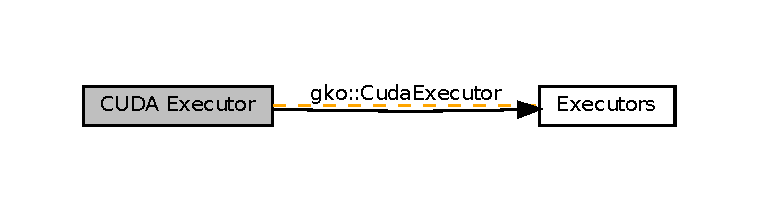
\includegraphics[width=350pt]{group__exec__cuda}
\end{center}
\end{figure}
\subsection*{Classes}
\begin{DoxyCompactItemize}
\item 
class \hyperlink{classgko_1_1CudaExecutor}{gko\+::\+Cuda\+Executor}
\begin{DoxyCompactList}\small\item\em This is the \hyperlink{classgko_1_1Executor}{Executor} subclass which represents the C\+U\+DA device. \end{DoxyCompactList}\end{DoxyCompactItemize}


\subsection{Detailed Description}
A module dedicated to the implementation and usage of the C\+U\+DA executor in Ginkgo. 


\hypertarget{group__Executor}{}\doxysection{Executors}
\label{group__Executor}\index{Executors@{Executors}}


A module dedicated to the implementation and usage of the executors in Ginkgo.  


Collaboration diagram for Executors\+:
\nopagebreak
\begin{figure}[H]
\begin{center}
\leavevmode
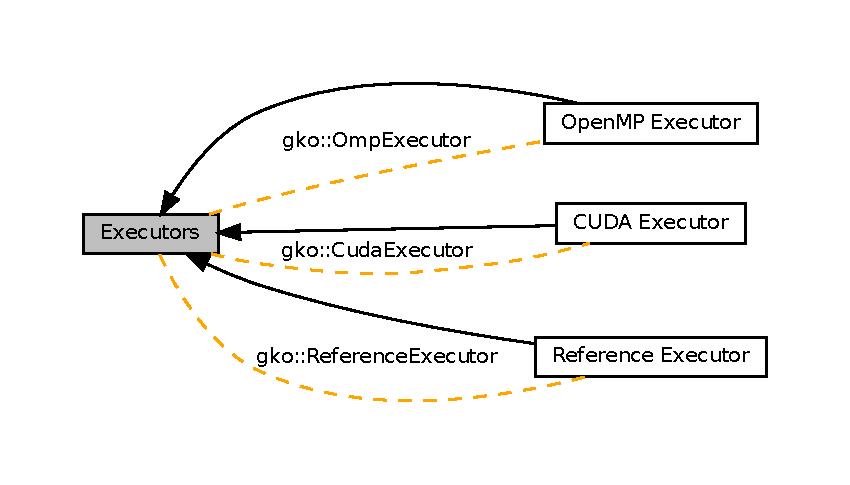
\includegraphics[width=350pt]{group__Executor}
\end{center}
\end{figure}
\doxysubsection*{Modules}
\begin{DoxyCompactItemize}
\item 
\mbox{\hyperlink{group__exec__cuda}{C\+U\+D\+A Executor}}
\begin{DoxyCompactList}\small\item\em A module dedicated to the implementation and usage of the C\+U\+DA executor in Ginkgo. \end{DoxyCompactList}\item 
\mbox{\hyperlink{group__exec__hip}{H\+I\+P Executor}}
\begin{DoxyCompactList}\small\item\em A module dedicated to the implementation and usage of the H\+IP executor in Ginkgo. \end{DoxyCompactList}\item 
\mbox{\hyperlink{group__exec__omp}{Open\+M\+P Executor}}
\begin{DoxyCompactList}\small\item\em A module dedicated to the implementation and usage of the Open\+MP executor in Ginkgo. \end{DoxyCompactList}\item 
\mbox{\hyperlink{group__exec__ref}{Reference Executor}}
\begin{DoxyCompactList}\small\item\em A module dedicated to the implementation and usage of the Reference executor in Ginkgo. \end{DoxyCompactList}\end{DoxyCompactItemize}
\doxysubsection*{Classes}
\begin{DoxyCompactItemize}
\item 
class \mbox{\hyperlink{classgko_1_1Operation}{gko\+::\+Operation}}
\begin{DoxyCompactList}\small\item\em Operations can be used to define functionalities whose implementations differ among devices. \end{DoxyCompactList}\item 
class \mbox{\hyperlink{classgko_1_1Executor}{gko\+::\+Executor}}
\begin{DoxyCompactList}\small\item\em The first step in using the Ginkgo library consists of creating an executor. \end{DoxyCompactList}\item 
class \mbox{\hyperlink{classgko_1_1executor__deleter}{gko\+::executor\+\_\+deleter$<$ T $>$}}
\begin{DoxyCompactList}\small\item\em This is a deleter that uses an executor\textquotesingle{}s {\ttfamily free} method to deallocate the data. \end{DoxyCompactList}\item 
class \mbox{\hyperlink{classgko_1_1OmpExecutor}{gko\+::\+Omp\+Executor}}
\begin{DoxyCompactList}\small\item\em This is the \mbox{\hyperlink{classgko_1_1Executor}{Executor}} subclass which represents the Open\+MP device (typically C\+PU). \end{DoxyCompactList}\item 
class \mbox{\hyperlink{classgko_1_1ReferenceExecutor}{gko\+::\+Reference\+Executor}}
\begin{DoxyCompactList}\small\item\em This is a specialization of the \mbox{\hyperlink{classgko_1_1OmpExecutor}{Omp\+Executor}}, which runs the reference implementations of the kernels used for debugging purposes. \end{DoxyCompactList}\item 
class \mbox{\hyperlink{classgko_1_1CudaExecutor}{gko\+::\+Cuda\+Executor}}
\begin{DoxyCompactList}\small\item\em This is the \mbox{\hyperlink{classgko_1_1Executor}{Executor}} subclass which represents the C\+U\+DA device. \end{DoxyCompactList}\item 
class \mbox{\hyperlink{classgko_1_1HipExecutor}{gko\+::\+Hip\+Executor}}
\begin{DoxyCompactList}\small\item\em This is the \mbox{\hyperlink{classgko_1_1Executor}{Executor}} subclass which represents the H\+IP enhanced device. \end{DoxyCompactList}\end{DoxyCompactItemize}
\doxysubsection*{Macros}
\begin{DoxyCompactItemize}
\item 
\#define \mbox{\hyperlink{group__Executor_ga7f2c119ff9f4f51c7f8e2d5dbbbbd044}{G\+K\+O\+\_\+\+R\+E\+G\+I\+S\+T\+E\+R\+\_\+\+O\+P\+E\+R\+A\+T\+I\+ON}}(\+\_\+name,  \+\_\+kernel)
\begin{DoxyCompactList}\small\item\em Binds a set of device-\/specific kernels to an Operation. \end{DoxyCompactList}\end{DoxyCompactItemize}


\doxysubsection{Detailed Description}
A module dedicated to the implementation and usage of the executors in Ginkgo. 

Below, we provide a brief introduction to executors in Ginkgo, how they have been implemented, how to best make use of them and how to add new executors.\hypertarget{group__Executor_exec_1}{}\doxysubsection{Executors in Ginkgo.}\label{group__Executor_exec_1}
The first step in using the Ginkgo library consists of creating an executor. Executors are used to specify the location for the data of linear algebra objects, and to determine where the operations will be executed. Ginkgo currently supports three different executor types\+:


\begin{DoxyItemize}
\item \mbox{\hyperlink{group__exec__omp}{Open\+MP Executor}} specifies that the data should be stored and the associated operations executed on an Open\+M\+P-\/supporting device (e.\+g. host C\+PU);
\item \mbox{\hyperlink{group__exec__cuda}{C\+U\+DA Executor}} specifies that the data should be stored and the operations executed on the N\+V\+I\+D\+IA G\+PU accelerator;
\item \mbox{\hyperlink{group__exec__hip}{H\+IP Executor}} uses the H\+IP library to compile code for either N\+V\+I\+D\+IA or A\+MD G\+PU accelerator;
\item \mbox{\hyperlink{group__exec__ref}{Reference Executor}} executes a non-\/optimized reference implementation, which can be used to debug the library. 
\end{DoxyItemize}

\doxysubsection{Macro Definition Documentation}
\mbox{\Hypertarget{group__Executor_ga7f2c119ff9f4f51c7f8e2d5dbbbbd044}\label{group__Executor_ga7f2c119ff9f4f51c7f8e2d5dbbbbd044}} 
\index{Executors@{Executors}!GKO\_REGISTER\_OPERATION@{GKO\_REGISTER\_OPERATION}}
\index{GKO\_REGISTER\_OPERATION@{GKO\_REGISTER\_OPERATION}!Executors@{Executors}}
\doxysubsubsection{\texorpdfstring{GKO\_REGISTER\_OPERATION}{GKO\_REGISTER\_OPERATION}}
{\footnotesize\ttfamily \#define G\+K\+O\+\_\+\+R\+E\+G\+I\+S\+T\+E\+R\+\_\+\+O\+P\+E\+R\+A\+T\+I\+ON(\begin{DoxyParamCaption}\item[{}]{\+\_\+name,  }\item[{}]{\+\_\+kernel }\end{DoxyParamCaption})}



Binds a set of device-\/specific kernels to an Operation. 

It also defines a helper function which creates the associated operation. Any input arguments passed to the helper function are forwarded to the kernel when the operation is executed.

The kernels used to bind the operation are searched in {\ttfamily kernels\+::\+D\+E\+V\+\_\+\+T\+Y\+PE} namespace, where {\ttfamily D\+E\+V\+\_\+\+T\+Y\+PE} is replaced by {\ttfamily omp}, {\ttfamily cuda}, {\ttfamily hip} and {\ttfamily reference}.


\begin{DoxyParams}{Parameters}
{\em \+\_\+name} & operation name \\
\hline
{\em \+\_\+kernel} & kernel which will be bound to the operation\\
\hline
\end{DoxyParams}
\hypertarget{group__Executor_autotoc_md64}{}\doxysubsubsection{Example}\label{group__Executor_autotoc_md64}

\begin{DoxyCode}{0}
\DoxyCodeLine{ \{c++\}}
\DoxyCodeLine{\textcolor{comment}{// define the omp, cuda, hip and reference kernels which will be bound to the}}
\DoxyCodeLine{\textcolor{comment}{// operation}}
\DoxyCodeLine{\textcolor{keyword}{namespace }kernels \{}
\DoxyCodeLine{\textcolor{keyword}{namespace }omp \{}
\DoxyCodeLine{\textcolor{keywordtype}{void} my\_kernel(\textcolor{keywordtype}{int} x) \{}
\DoxyCodeLine{     \textcolor{comment}{// omp code}}
\DoxyCodeLine{\}}
\DoxyCodeLine{\}}
\DoxyCodeLine{\textcolor{keyword}{namespace }cuda \{}
\DoxyCodeLine{\textcolor{keywordtype}{void} my\_kernel(\textcolor{keywordtype}{int} x) \{}
\DoxyCodeLine{     \textcolor{comment}{// cuda code}}
\DoxyCodeLine{\}}
\DoxyCodeLine{\}}
\DoxyCodeLine{\textcolor{keyword}{namespace }hip \{}
\DoxyCodeLine{\textcolor{keywordtype}{void} my\_kernel(\textcolor{keywordtype}{int} x) \{}
\DoxyCodeLine{     \textcolor{comment}{// hip code}}
\DoxyCodeLine{\}}
\DoxyCodeLine{\}}
\DoxyCodeLine{\textcolor{keyword}{namespace }reference \{}
\DoxyCodeLine{\textcolor{keywordtype}{void} my\_kernel(\textcolor{keywordtype}{int} x) \{}
\DoxyCodeLine{    \textcolor{comment}{// reference code}}
\DoxyCodeLine{\}}
\DoxyCodeLine{\}}
\DoxyCodeLine{}
\DoxyCodeLine{\textcolor{comment}{// Bind the kernels to the operation}}
\DoxyCodeLine{\mbox{\hyperlink{group__Executor_ga7f2c119ff9f4f51c7f8e2d5dbbbbd044}{GKO\_REGISTER\_OPERATION}}(my\_op, my\_kernel);}
\DoxyCodeLine{}
\DoxyCodeLine{\textcolor{keywordtype}{int} main() \{}
\DoxyCodeLine{    \textcolor{comment}{// create executors}}
\DoxyCodeLine{    \textcolor{keyword}{auto} omp = OmpExecutor::create();}
\DoxyCodeLine{    \textcolor{keyword}{auto} cuda = CudaExecutor::create(omp, 0);}
\DoxyCodeLine{    \textcolor{keyword}{auto} hip = HipExecutor::create(omp, 0);}
\DoxyCodeLine{    \textcolor{keyword}{auto} ref = ReferenceExecutor::create();}
\DoxyCodeLine{}
\DoxyCodeLine{    \textcolor{comment}{// create the operation}}
\DoxyCodeLine{    \textcolor{keyword}{auto} op = make\_my\_op(5); \textcolor{comment}{// x = 5}}
\DoxyCodeLine{}
\DoxyCodeLine{    omp-\/>run(op);  \textcolor{comment}{// run omp kernel}}
\DoxyCodeLine{    cuda-\/>run(op);  \textcolor{comment}{// run cuda kernel}}
\DoxyCodeLine{    hip-\/>run(op);  \textcolor{comment}{// run hip kernel}}
\DoxyCodeLine{    ref-\/>run(op);  \textcolor{comment}{// run reference kernel}}
\DoxyCodeLine{\}}
\end{DoxyCode}
 
\hypertarget{group__LinOp}{}\doxysection{Linear Operators}
\label{group__LinOp}\index{Linear Operators@{Linear Operators}}


A module dedicated to the implementation and usage of the Linear operators in Ginkgo.  


Collaboration diagram for Linear Operators\+:
\nopagebreak
\begin{figure}[H]
\begin{center}
\leavevmode
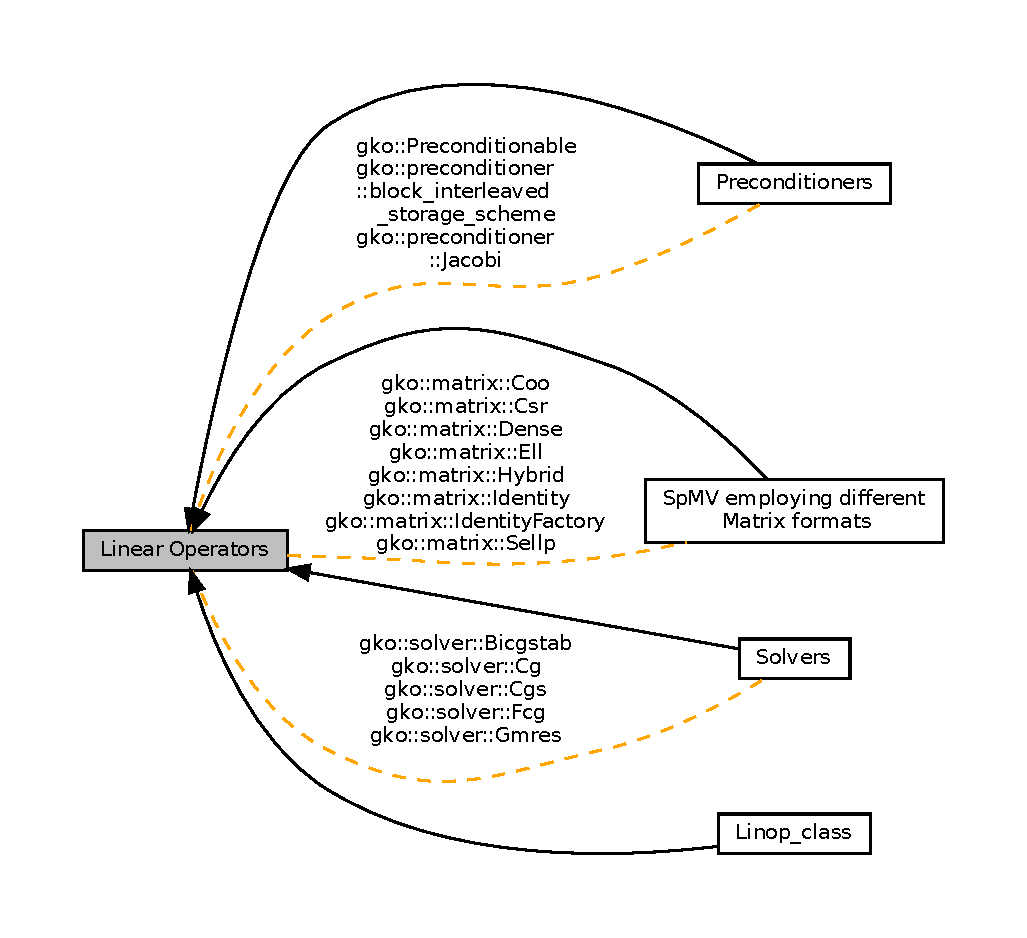
\includegraphics[width=350pt]{group__LinOp}
\end{center}
\end{figure}
\doxysubsection*{Modules}
\begin{DoxyCompactItemize}
\item 
\mbox{\hyperlink{group__factor}{Factorizations}}
\begin{DoxyCompactList}\small\item\em A module dedicated to the implementation and usage of the Factorizations in Ginkgo. \end{DoxyCompactList}\item 
\mbox{\hyperlink{group__mat__formats}{Sp\+M\+V employing different Matrix formats}}
\begin{DoxyCompactList}\small\item\em A module dedicated to the implementation and usage of the various Matrix Formats in Ginkgo. \end{DoxyCompactList}\item 
\mbox{\hyperlink{group__precond}{Preconditioners}}
\begin{DoxyCompactList}\small\item\em A module dedicated to the implementation and usage of the Preconditioners in Ginkgo. \end{DoxyCompactList}\item 
\mbox{\hyperlink{group__solvers}{Solvers}}
\begin{DoxyCompactList}\small\item\em A module dedicated to the implementation and usage of the Solvers in Ginkgo. \end{DoxyCompactList}\end{DoxyCompactItemize}
\doxysubsection*{Classes}
\begin{DoxyCompactItemize}
\item 
class \mbox{\hyperlink{classgko_1_1Combination}{gko\+::\+Combination$<$ Value\+Type $>$}}
\begin{DoxyCompactList}\small\item\em The \mbox{\hyperlink{classgko_1_1Combination}{Combination}} class can be used to construct a linear combination of multiple linear operators {\ttfamily c1 $\ast$ op1 + c2 $\ast$ op2 + ... }\end{DoxyCompactList}\item 
class \mbox{\hyperlink{classgko_1_1Composition}{gko\+::\+Composition$<$ Value\+Type $>$}}
\begin{DoxyCompactList}\small\item\em The \mbox{\hyperlink{classgko_1_1Composition}{Composition}} class can be used to compose linear operators {\ttfamily op1, op2, ..., opn} and obtain the operator {\ttfamily op1 $\ast$ op2 $\ast$ ... }\end{DoxyCompactList}\item 
class \mbox{\hyperlink{classgko_1_1LinOpFactory}{gko\+::\+Lin\+Op\+Factory}}
\begin{DoxyCompactList}\small\item\em A \mbox{\hyperlink{classgko_1_1LinOpFactory}{Lin\+Op\+Factory}} represents a higher order mapping which transforms one linear operator into another. \end{DoxyCompactList}\item 
class \mbox{\hyperlink{classgko_1_1ReadableFromMatrixData}{gko\+::\+Readable\+From\+Matrix\+Data$<$ Value\+Type, Index\+Type $>$}}
\begin{DoxyCompactList}\small\item\em A \mbox{\hyperlink{classgko_1_1LinOp}{Lin\+Op}} implementing this interface can read its data from a \mbox{\hyperlink{structgko_1_1matrix__data}{matrix\+\_\+data}} structure. \end{DoxyCompactList}\item 
class \mbox{\hyperlink{classgko_1_1WritableToMatrixData}{gko\+::\+Writable\+To\+Matrix\+Data$<$ Value\+Type, Index\+Type $>$}}
\begin{DoxyCompactList}\small\item\em A \mbox{\hyperlink{classgko_1_1LinOp}{Lin\+Op}} implementing this interface can write its data to a \mbox{\hyperlink{structgko_1_1matrix__data}{matrix\+\_\+data}} structure. \end{DoxyCompactList}\item 
class \mbox{\hyperlink{classgko_1_1Preconditionable}{gko\+::\+Preconditionable}}
\begin{DoxyCompactList}\small\item\em A \mbox{\hyperlink{classgko_1_1LinOp}{Lin\+Op}} implementing this interface can be preconditioned. \end{DoxyCompactList}\item 
class \mbox{\hyperlink{classgko_1_1DiagonalExtractable}{gko\+::\+Diagonal\+Extractable$<$ Value\+Type $>$}}
\begin{DoxyCompactList}\small\item\em The diagonal of a \mbox{\hyperlink{classgko_1_1LinOp}{Lin\+Op}} implementing this interface can be extracted. \end{DoxyCompactList}\item 
class \mbox{\hyperlink{classgko_1_1EnableAbsoluteComputation}{gko\+::\+Enable\+Absolute\+Computation$<$ Absolute\+Lin\+Op $>$}}
\begin{DoxyCompactList}\small\item\em The \mbox{\hyperlink{classgko_1_1EnableAbsoluteComputation}{Enable\+Absolute\+Computation}} mixin provides the default implementations of {\ttfamily compute\+\_\+absolute\+\_\+linop} and the absolute interface. \end{DoxyCompactList}\item 
class \mbox{\hyperlink{classgko_1_1EnableLinOp}{gko\+::\+Enable\+Lin\+Op$<$ Concrete\+Lin\+Op, Polymorphic\+Base $>$}}
\begin{DoxyCompactList}\small\item\em The \mbox{\hyperlink{classgko_1_1EnableLinOp}{Enable\+Lin\+Op}} mixin can be used to provide sensible default implementations of the majority of the \mbox{\hyperlink{classgko_1_1LinOp}{Lin\+Op}} and \mbox{\hyperlink{classgko_1_1PolymorphicObject}{Polymorphic\+Object}} interface. \end{DoxyCompactList}\item 
class \mbox{\hyperlink{classgko_1_1Perturbation}{gko\+::\+Perturbation$<$ Value\+Type $>$}}
\begin{DoxyCompactList}\small\item\em The \mbox{\hyperlink{classgko_1_1Perturbation}{Perturbation}} class can be used to construct a \mbox{\hyperlink{classgko_1_1LinOp}{Lin\+Op}} to represent the operation {\ttfamily (identity + scalar $\ast$ basis $\ast$ projector)}. \end{DoxyCompactList}\item 
class \mbox{\hyperlink{classgko_1_1factorization_1_1Ilu}{gko\+::factorization\+::\+Ilu$<$ Value\+Type, Index\+Type $>$}}
\begin{DoxyCompactList}\small\item\em Represents an incomplete LU factorization -- I\+L\+U(0) -- of a sparse matrix. \end{DoxyCompactList}\item 
class \mbox{\hyperlink{classgko_1_1factorization_1_1ParIct}{gko\+::factorization\+::\+Par\+Ict$<$ Value\+Type, Index\+Type $>$}}
\begin{DoxyCompactList}\small\item\em Par\+I\+CT is an incomplete threshold-\/based Cholesky factorization which is computed in parallel. \end{DoxyCompactList}\item 
class \mbox{\hyperlink{classgko_1_1factorization_1_1ParIlu}{gko\+::factorization\+::\+Par\+Ilu$<$ Value\+Type, Index\+Type $>$}}
\begin{DoxyCompactList}\small\item\em Par\+I\+LU is an incomplete LU factorization which is computed in parallel. \end{DoxyCompactList}\item 
class \mbox{\hyperlink{classgko_1_1factorization_1_1ParIlut}{gko\+::factorization\+::\+Par\+Ilut$<$ Value\+Type, Index\+Type $>$}}
\begin{DoxyCompactList}\small\item\em Par\+I\+L\+UT is an incomplete threshold-\/based LU factorization which is computed in parallel. \end{DoxyCompactList}\item 
class \mbox{\hyperlink{classgko_1_1matrix_1_1Coo}{gko\+::matrix\+::\+Coo$<$ Value\+Type, Index\+Type $>$}}
\begin{DoxyCompactList}\small\item\em C\+OO stores a matrix in the coordinate matrix format. \end{DoxyCompactList}\item 
class \mbox{\hyperlink{classgko_1_1matrix_1_1Csr}{gko\+::matrix\+::\+Csr$<$ Value\+Type, Index\+Type $>$}}
\begin{DoxyCompactList}\small\item\em C\+SR is a matrix format which stores only the nonzero coefficients by compressing each row of the matrix (compressed sparse row format). \end{DoxyCompactList}\item 
class \mbox{\hyperlink{classgko_1_1matrix_1_1Dense}{gko\+::matrix\+::\+Dense$<$ Value\+Type $>$}}
\begin{DoxyCompactList}\small\item\em \mbox{\hyperlink{classgko_1_1matrix_1_1Dense}{Dense}} is a matrix format which explicitly stores all values of the matrix. \end{DoxyCompactList}\item 
class \mbox{\hyperlink{classgko_1_1matrix_1_1Diagonal}{gko\+::matrix\+::\+Diagonal$<$ Value\+Type $>$}}
\begin{DoxyCompactList}\small\item\em This class is a utility which efficiently implements the diagonal matrix (a linear operator which scales a vector row wise). \end{DoxyCompactList}\item 
class \mbox{\hyperlink{classgko_1_1matrix_1_1Ell}{gko\+::matrix\+::\+Ell$<$ Value\+Type, Index\+Type $>$}}
\begin{DoxyCompactList}\small\item\em E\+LL is a matrix format where stride with explicit zeros is used such that all rows have the same number of stored elements. \end{DoxyCompactList}\item 
class \mbox{\hyperlink{classgko_1_1matrix_1_1Hybrid}{gko\+::matrix\+::\+Hybrid$<$ Value\+Type, Index\+Type $>$}}
\begin{DoxyCompactList}\small\item\em H\+Y\+B\+R\+ID is a matrix format which splits the matrix into E\+L\+L\+P\+A\+CK and C\+OO format. \end{DoxyCompactList}\item 
class \mbox{\hyperlink{classgko_1_1matrix_1_1Identity}{gko\+::matrix\+::\+Identity$<$ Value\+Type $>$}}
\begin{DoxyCompactList}\small\item\em This class is a utility which efficiently implements the identity matrix (a linear operator which maps each vector to itself). \end{DoxyCompactList}\item 
class \mbox{\hyperlink{classgko_1_1matrix_1_1IdentityFactory}{gko\+::matrix\+::\+Identity\+Factory$<$ Value\+Type $>$}}
\begin{DoxyCompactList}\small\item\em This factory is a utility which can be used to generate \mbox{\hyperlink{classgko_1_1matrix_1_1Identity}{Identity}} operators. \end{DoxyCompactList}\item 
class \mbox{\hyperlink{classgko_1_1matrix_1_1Permutation}{gko\+::matrix\+::\+Permutation$<$ Index\+Type $>$}}
\begin{DoxyCompactList}\small\item\em \mbox{\hyperlink{classgko_1_1matrix_1_1Permutation}{Permutation}} is a matrix \char`\"{}format\char`\"{} which stores the row and column permutation arrays which can be used for re-\/ordering the rows and columns a matrix. \end{DoxyCompactList}\item 
class \mbox{\hyperlink{classgko_1_1matrix_1_1Sellp}{gko\+::matrix\+::\+Sellp$<$ Value\+Type, Index\+Type $>$}}
\begin{DoxyCompactList}\small\item\em S\+E\+L\+L-\/P is a matrix format similar to E\+LL format. \end{DoxyCompactList}\item 
class \mbox{\hyperlink{classgko_1_1matrix_1_1SparsityCsr}{gko\+::matrix\+::\+Sparsity\+Csr$<$ Value\+Type, Index\+Type $>$}}
\begin{DoxyCompactList}\small\item\em \mbox{\hyperlink{classgko_1_1matrix_1_1SparsityCsr}{Sparsity\+Csr}} is a matrix format which stores only the sparsity pattern of a sparse matrix by compressing each row of the matrix (compressed sparse row format). \end{DoxyCompactList}\item 
class \mbox{\hyperlink{classgko_1_1preconditioner_1_1Ilu}{gko\+::preconditioner\+::\+Ilu$<$ L\+Solver\+Type, U\+Solver\+Type, Reverse\+Apply, Index\+Type $>$}}
\begin{DoxyCompactList}\small\item\em The Incomplete LU (I\+LU) preconditioner solves the equation $LUx = b$ for a given lower triangular matrix L, an upper triangular matrix U and the right hand side b (can contain multiple right hand sides). \end{DoxyCompactList}\item 
class \mbox{\hyperlink{classgko_1_1preconditioner_1_1Isai}{gko\+::preconditioner\+::\+Isai$<$ Isai\+Type, Value\+Type, Index\+Type $>$}}
\begin{DoxyCompactList}\small\item\em The Incomplete Sparse Approximate Inverse (I\+S\+AI) Preconditioner generates an approximate inverse matrix for a given lower triangular matrix L or upper triangular matrix U. \end{DoxyCompactList}\item 
class \mbox{\hyperlink{classgko_1_1preconditioner_1_1Jacobi}{gko\+::preconditioner\+::\+Jacobi$<$ Value\+Type, Index\+Type $>$}}
\begin{DoxyCompactList}\small\item\em A block-\/\+Jacobi preconditioner is a block-\/diagonal linear operator, obtained by inverting the diagonal blocks of the source operator. \end{DoxyCompactList}\item 
class \mbox{\hyperlink{classgko_1_1solver_1_1Bicg}{gko\+::solver\+::\+Bicg$<$ Value\+Type $>$}}
\begin{DoxyCompactList}\small\item\em B\+I\+CG or the Biconjugate gradient method is a Krylov subspace solver. \end{DoxyCompactList}\item 
class \mbox{\hyperlink{classgko_1_1solver_1_1Bicgstab}{gko\+::solver\+::\+Bicgstab$<$ Value\+Type $>$}}
\begin{DoxyCompactList}\small\item\em Bi\+C\+G\+S\+T\+AB or the Bi-\/\+Conjugate Gradient-\/\+Stabilized is a Krylov subspace solver. \end{DoxyCompactList}\item 
class \mbox{\hyperlink{classgko_1_1solver_1_1Cg}{gko\+::solver\+::\+Cg$<$ Value\+Type $>$}}
\begin{DoxyCompactList}\small\item\em CG or the conjugate gradient method is an iterative type Krylov subspace method which is suitable for symmetric positive definite methods. \end{DoxyCompactList}\item 
class \mbox{\hyperlink{classgko_1_1solver_1_1Cgs}{gko\+::solver\+::\+Cgs$<$ Value\+Type $>$}}
\begin{DoxyCompactList}\small\item\em C\+GS or the conjugate gradient square method is an iterative type Krylov subspace method which is suitable for general systems. \end{DoxyCompactList}\item 
class \mbox{\hyperlink{classgko_1_1solver_1_1Fcg}{gko\+::solver\+::\+Fcg$<$ Value\+Type $>$}}
\begin{DoxyCompactList}\small\item\em F\+CG or the flexible conjugate gradient method is an iterative type Krylov subspace method which is suitable for symmetric positive definite methods. \end{DoxyCompactList}\item 
class \mbox{\hyperlink{classgko_1_1solver_1_1Gmres}{gko\+::solver\+::\+Gmres$<$ Value\+Type $>$}}
\begin{DoxyCompactList}\small\item\em G\+M\+R\+ES or the generalized minimal residual method is an iterative type Krylov subspace method which is suitable for nonsymmetric linear systems. \end{DoxyCompactList}\item 
class \mbox{\hyperlink{classgko_1_1solver_1_1Ir}{gko\+::solver\+::\+Ir$<$ Value\+Type $>$}}
\begin{DoxyCompactList}\small\item\em Iterative refinement (IR) is an iterative method that uses another coarse method to approximate the error of the current solution via the current residual. \end{DoxyCompactList}\item 
class \mbox{\hyperlink{classgko_1_1solver_1_1LowerTrs}{gko\+::solver\+::\+Lower\+Trs$<$ Value\+Type, Index\+Type $>$}}
\begin{DoxyCompactList}\small\item\em \mbox{\hyperlink{classgko_1_1solver_1_1LowerTrs}{Lower\+Trs}} is the triangular solver which solves the system L x = b, when L is a lower triangular matrix. \end{DoxyCompactList}\item 
class \mbox{\hyperlink{classgko_1_1solver_1_1UpperTrs}{gko\+::solver\+::\+Upper\+Trs$<$ Value\+Type, Index\+Type $>$}}
\begin{DoxyCompactList}\small\item\em \mbox{\hyperlink{classgko_1_1solver_1_1UpperTrs}{Upper\+Trs}} is the triangular solver which solves the system U x = b, when U is an upper triangular matrix. \end{DoxyCompactList}\end{DoxyCompactItemize}
\doxysubsection*{Macros}
\begin{DoxyCompactItemize}
\item 
\#define \mbox{\hyperlink{group__LinOp_ga1fc8e9d8be0c9ad2d72bc1ddfc6d8358}{G\+K\+O\+\_\+\+C\+R\+E\+A\+T\+E\+\_\+\+F\+A\+C\+T\+O\+R\+Y\+\_\+\+P\+A\+R\+A\+M\+E\+T\+E\+RS}}(\+\_\+parameters\+\_\+name,  \+\_\+factory\+\_\+name)
\begin{DoxyCompactList}\small\item\em This Macro will generate a new type containing the parameters for the factory {\ttfamily \+\_\+factory\+\_\+name}. \end{DoxyCompactList}\item 
\#define \mbox{\hyperlink{group__LinOp_ga8e0af90ec2414b768266f77cedffc309}{G\+K\+O\+\_\+\+E\+N\+A\+B\+L\+E\+\_\+\+L\+I\+N\+\_\+\+O\+P\+\_\+\+F\+A\+C\+T\+O\+RY}}(\+\_\+lin\+\_\+op,  \+\_\+parameters\+\_\+name,  \+\_\+factory\+\_\+name)
\begin{DoxyCompactList}\small\item\em This macro will generate a default implementation of a Lin\+Op\+Factory for the Lin\+Op subclass it is defined in. \end{DoxyCompactList}\item 
\#define \mbox{\hyperlink{group__LinOp_ga521f65604cc4cf427dcb2ecfa49b757c}{G\+K\+O\+\_\+\+E\+N\+A\+B\+L\+E\+\_\+\+B\+U\+I\+L\+D\+\_\+\+M\+E\+T\+H\+OD}}(\+\_\+factory\+\_\+name)
\begin{DoxyCompactList}\small\item\em Defines a build method for the factory, simplifying its construction by removing the repetitive typing of factory\textquotesingle{}s name. \end{DoxyCompactList}\item 
\#define \mbox{\hyperlink{group__LinOp_gaa037309884bbd0562b897cee95dd91c8}{G\+K\+O\+\_\+\+F\+A\+C\+T\+O\+R\+Y\+\_\+\+P\+A\+R\+A\+M\+E\+T\+ER}}(\+\_\+name, ...)
\begin{DoxyCompactList}\small\item\em Creates a factory parameter in the factory parameters structure. \end{DoxyCompactList}\item 
\#define \mbox{\hyperlink{group__LinOp_ga49d4c09c39f06b22bebbbfd1d8bfe450}{G\+K\+O\+\_\+\+F\+A\+C\+T\+O\+R\+Y\+\_\+\+P\+A\+R\+A\+M\+E\+T\+E\+R\+\_\+\+S\+C\+A\+L\+AR}}(\+\_\+name,  \+\_\+default)~\mbox{\hyperlink{group__LinOp_gaa037309884bbd0562b897cee95dd91c8}{G\+K\+O\+\_\+\+F\+A\+C\+T\+O\+R\+Y\+\_\+\+P\+A\+R\+A\+M\+E\+T\+ER}}(\+\_\+name, \+\_\+default)
\begin{DoxyCompactList}\small\item\em Creates a scalar factory parameter in the factory parameters structure. \end{DoxyCompactList}\item 
\#define \mbox{\hyperlink{group__LinOp_gaa292314d27ec1fb7ad54debaa3606ea8}{G\+K\+O\+\_\+\+F\+A\+C\+T\+O\+R\+Y\+\_\+\+P\+A\+R\+A\+M\+E\+T\+E\+R\+\_\+\+V\+E\+C\+T\+OR}}(\+\_\+name, ...)~\mbox{\hyperlink{group__LinOp_gaa037309884bbd0562b897cee95dd91c8}{G\+K\+O\+\_\+\+F\+A\+C\+T\+O\+R\+Y\+\_\+\+P\+A\+R\+A\+M\+E\+T\+ER}}(\+\_\+name, \+\_\+\+\_\+\+V\+A\+\_\+\+A\+R\+G\+S\+\_\+\+\_\+)
\begin{DoxyCompactList}\small\item\em Creates a vector factory parameter in the factory parameters structure. \end{DoxyCompactList}\end{DoxyCompactItemize}
\doxysubsection*{Typedefs}
\begin{DoxyCompactItemize}
\item 
{\footnotesize template$<$typename Concrete\+Factory , typename Concrete\+Lin\+Op , typename Parameters\+Type , typename Polymorphic\+Base  = Lin\+Op\+Factory$>$ }\\using \mbox{\hyperlink{group__LinOp_ga24628d477cba68b31cea690572c51912}{gko\+::\+Enable\+Default\+Lin\+Op\+Factory}} = \mbox{\hyperlink{classgko_1_1EnableDefaultFactory}{Enable\+Default\+Factory}}$<$ Concrete\+Factory, Concrete\+Lin\+Op, Parameters\+Type, Polymorphic\+Base $>$
\begin{DoxyCompactList}\small\item\em This is an alias for the \mbox{\hyperlink{classgko_1_1EnableDefaultFactory}{Enable\+Default\+Factory}} mixin, which correctly sets the template parameters to enable a subclass of \mbox{\hyperlink{classgko_1_1LinOpFactory}{Lin\+Op\+Factory}}. \end{DoxyCompactList}\end{DoxyCompactItemize}


\doxysubsection{Detailed Description}
A module dedicated to the implementation and usage of the Linear operators in Ginkgo. 

Below we elaborate on one of the most important concepts of Ginkgo, the linear operator. The linear operator (\mbox{\hyperlink{classgko_1_1LinOp}{Lin\+Op}}) is a base class for all linear algebra objects in Ginkgo. The main benefit of having a single base class for the entire collection of linear algebra objects (as opposed to having separate hierarchies for matrices, solvers and preconditioners) is the generality it provides.\hypertarget{group__LinOp_linop_3}{}\doxysubsection{Advantages of this approach and usage}\label{group__LinOp_linop_3}
A common interface often allows for writing more generic code. If a user\textquotesingle{}s routine requires only operations provided by the \mbox{\hyperlink{classgko_1_1LinOp}{Lin\+Op}} interface, the same code can be used for any kind of linear operators, independent of whether these are matrices, solvers or preconditioners. This feature is also extensively used in Ginkgo itself. For example, a preconditioner used inside a Krylov solver is a \mbox{\hyperlink{classgko_1_1LinOp}{Lin\+Op}}. This allows the user to supply a wide variety of preconditioners\+: either the ones which were designed to be used in this scenario (like I\+LU or block-\/\+Jacobi), a user-\/supplied matrix which is known to be a good preconditioner for the specific problem, or even another solver (e.\+g., if constructing a flexible G\+M\+R\+ES solver).

For example, a matrix free implementation would require the user to provide an apply implementation and instead of passing the generated matrix to the solver, they would have to provide their apply implementation for all the executors needed and no other code needs to be changed. See \mbox{\hyperlink{custom_matrix_format}{The custom-\/matrix-\/format program}} example for more details.\hypertarget{group__LinOp_linop_concept}{}\doxysubsection{Linear operator as a concept}\label{group__LinOp_linop_concept}
The linear operator (\mbox{\hyperlink{classgko_1_1LinOp}{Lin\+Op}}) is a base class for all linear algebra objects in Ginkgo. The main benefit of having a single base class for the entire collection of linear algebra objects (as opposed to having separate hierarchies for matrices, solvers and preconditioners) is the generality it provides.

First, since all subclasses provide a common interface, the library users are exposed to a smaller set of routines. For example, a matrix-\/vector product, a preconditioner application, or even a system solve are just different terms given to the operation of applying a certain linear operator to a vector. As such, Ginkgo uses the same routine name, \mbox{\hyperlink{classgko_1_1LinOp_a0449b2fc705d2f970855af23b5e2788e}{Lin\+Op\+::apply()}} for each of these operations, where the actual operation performed depends on the type of linear operator involved in the operation.

Second, a common interface often allows for writing more generic code. If a user\textquotesingle{}s routine requires only operations provided by the \mbox{\hyperlink{classgko_1_1LinOp}{Lin\+Op}} interface, the same code can be used for any kind of linear operators, independent of whether these are matrices, solvers or preconditioners. This feature is also extensively used in Ginkgo itself. For example, a preconditioner used inside a Krylov solver is a \mbox{\hyperlink{classgko_1_1LinOp}{Lin\+Op}}. This allows the user to supply a wide variety of preconditioners\+: either the ones which were designed to be used in this scenario (like I\+LU or block-\/\+Jacobi), a user-\/supplied matrix which is known to be a good preconditioner for the specific problem, or even another solver (e.\+g., if constructing a flexible G\+M\+R\+ES solver).

A key observation for providing a unified interface for matrices, solvers, and preconditioners is that the most common operation performed on all of them can be expressed as an application of a linear operator to a vector\+:


\begin{DoxyItemize}
\item the sparse matrix-\/vector product with a matrix $A$ is a linear operator application $y = Ax$;
\item the application of a preconditioner is a linear operator application $y = M^{-1}x$, where $M$ is an approximation of the original system matrix $A$ (thus a preconditioner represents an \char`\"{}approximate
    inverse\char`\"{} operator $M^{-1}$).
\item the system solve $Ax = b$ can be viewed as linear operator application $x = A^{-1}b$ (it goes without saying that the implementation of linear system solves does not follow this conceptual idea), so a linear system solver can be viewed as a representation of the operator $A^{-1}$.
\end{DoxyItemize}

Finally, direct manipulation of \mbox{\hyperlink{classgko_1_1LinOp}{Lin\+Op}} objects is rarely required in simple scenarios. As an illustrative example, one could construct a fixed-\/point iteration routine $x_{k+1} = Lx_k + b$ as follows\+:


\begin{DoxyCode}{0}
\DoxyCodeLine{std::unique\_ptr<matrix::Dense<>> calculate\_fixed\_point(}
\DoxyCodeLine{        \textcolor{keywordtype}{int} iters, \textcolor{keyword}{const} LinOp *L, \textcolor{keyword}{const} matrix::Dense<> *x0}
\DoxyCodeLine{        \textcolor{keyword}{const} matrix::Dense<> *b)}
\DoxyCodeLine{\{}
\DoxyCodeLine{    \textcolor{keyword}{auto} x = \mbox{\hyperlink{namespacegko_a1beb80750459e4201aa9d882d2d074c3}{gko::clone}}(x0);}
\DoxyCodeLine{    \textcolor{keyword}{auto} tmp = \mbox{\hyperlink{namespacegko_a1beb80750459e4201aa9d882d2d074c3}{gko::clone}}(x0);}
\DoxyCodeLine{    \textcolor{keyword}{auto} \mbox{\hyperlink{namespacegko_a0059e27f8f4bc348ff65c1e60caf47c8}{one}} = Dense<>::create(L-\/>get\_executor(), \{1.0,\});}
\DoxyCodeLine{    \textcolor{keywordflow}{for} (\textcolor{keywordtype}{int} i = 0; i < iters; ++i) \{}
\DoxyCodeLine{        L-\/>apply(\mbox{\hyperlink{namespacegko_a4edc2273b5627ec552ea423b60493be3}{gko::lend}}(tmp), \mbox{\hyperlink{namespacegko_a4edc2273b5627ec552ea423b60493be3}{gko::lend}}(x));}
\DoxyCodeLine{        x-\/>add\_scaled(\mbox{\hyperlink{namespacegko_a4edc2273b5627ec552ea423b60493be3}{gko::lend}}(\mbox{\hyperlink{namespacegko_a0059e27f8f4bc348ff65c1e60caf47c8}{one}}), \mbox{\hyperlink{namespacegko_a4edc2273b5627ec552ea423b60493be3}{gko::lend}}(b));}
\DoxyCodeLine{        tmp-\/>copy\_from(\mbox{\hyperlink{namespacegko_a4edc2273b5627ec552ea423b60493be3}{gko::lend}}(x));}
\DoxyCodeLine{    \}}
\DoxyCodeLine{    \textcolor{keywordflow}{return} x;}
\DoxyCodeLine{\}}
\end{DoxyCode}


Here, if $L$ is a matrix, \mbox{\hyperlink{classgko_1_1LinOp_a0449b2fc705d2f970855af23b5e2788e}{Lin\+Op\+::apply()}} refers to the matrix vector product, and {\ttfamily L-\/$>$apply(a, b)} computes $b = L \cdot a$. {\ttfamily x-\/$>$add\+\_\+scaled(one.\+get(), b.\+get())} is the {\ttfamily axpy} vector update $x:=x+b$.

The interesting part of this example is the apply() routine at line 4 of the function body. Since this routine is part of the \mbox{\hyperlink{classgko_1_1LinOp}{Lin\+Op}} base class, the fixed-\/point iteration routine can calculate a fixed point not only for matrices, but for any type of linear operator.

\mbox{\hyperlink{group__LinOp}{Linear Operators}} 

\doxysubsection{Macro Definition Documentation}
\mbox{\Hypertarget{group__LinOp_ga1fc8e9d8be0c9ad2d72bc1ddfc6d8358}\label{group__LinOp_ga1fc8e9d8be0c9ad2d72bc1ddfc6d8358}} 
\index{Linear Operators@{Linear Operators}!GKO\_CREATE\_FACTORY\_PARAMETERS@{GKO\_CREATE\_FACTORY\_PARAMETERS}}
\index{GKO\_CREATE\_FACTORY\_PARAMETERS@{GKO\_CREATE\_FACTORY\_PARAMETERS}!Linear Operators@{Linear Operators}}
\doxysubsubsection{\texorpdfstring{GKO\_CREATE\_FACTORY\_PARAMETERS}{GKO\_CREATE\_FACTORY\_PARAMETERS}}
{\footnotesize\ttfamily \#define G\+K\+O\+\_\+\+C\+R\+E\+A\+T\+E\+\_\+\+F\+A\+C\+T\+O\+R\+Y\+\_\+\+P\+A\+R\+A\+M\+E\+T\+E\+RS(\begin{DoxyParamCaption}\item[{}]{\+\_\+parameters\+\_\+name,  }\item[{}]{\+\_\+factory\+\_\+name }\end{DoxyParamCaption})}

{\bfseries Value\+:}
\begin{DoxyCode}{0}
\DoxyCodeLine{\textcolor{keyword}{public}:                                                                \(\backslash\)}
\DoxyCodeLine{    class \_factory\_name;                                               \(\backslash\)}
\DoxyCodeLine{    struct \_parameters\_name\#\#\_type                                     \(\backslash\)}
\DoxyCodeLine{        : \mbox{\hyperlink{structgko_1_1enable__parameters__type}{::gko::enable\_parameters\_type}}<\_parameters\_name\#\#\_type,       \(\backslash\)}
\DoxyCodeLine{                                        \_factory\_name>}

\end{DoxyCode}


This Macro will generate a new type containing the parameters for the factory {\ttfamily \+\_\+factory\+\_\+name}. 

For more details, see \mbox{\hyperlink{group__LinOp_ga8e0af90ec2414b768266f77cedffc309}{G\+K\+O\+\_\+\+E\+N\+A\+B\+L\+E\+\_\+\+L\+I\+N\+\_\+\+O\+P\+\_\+\+F\+A\+C\+T\+O\+R\+Y()}}. It is required to use this macro {\bfseries{before}} calling the macro \mbox{\hyperlink{group__LinOp_ga8e0af90ec2414b768266f77cedffc309}{G\+K\+O\+\_\+\+E\+N\+A\+B\+L\+E\+\_\+\+L\+I\+N\+\_\+\+O\+P\+\_\+\+F\+A\+C\+T\+O\+R\+Y()}}. It is also required to use the same names for all parameters between both macros.


\begin{DoxyParams}{Parameters}
{\em \+\_\+parameters\+\_\+name} & name of the parameters member in the class \\
\hline
{\em \+\_\+factory\+\_\+name} & name of the generated factory type \\
\hline
\end{DoxyParams}
\mbox{\Hypertarget{group__LinOp_ga521f65604cc4cf427dcb2ecfa49b757c}\label{group__LinOp_ga521f65604cc4cf427dcb2ecfa49b757c}} 
\index{Linear Operators@{Linear Operators}!GKO\_ENABLE\_BUILD\_METHOD@{GKO\_ENABLE\_BUILD\_METHOD}}
\index{GKO\_ENABLE\_BUILD\_METHOD@{GKO\_ENABLE\_BUILD\_METHOD}!Linear Operators@{Linear Operators}}
\doxysubsubsection{\texorpdfstring{GKO\_ENABLE\_BUILD\_METHOD}{GKO\_ENABLE\_BUILD\_METHOD}}
{\footnotesize\ttfamily \#define G\+K\+O\+\_\+\+E\+N\+A\+B\+L\+E\+\_\+\+B\+U\+I\+L\+D\+\_\+\+M\+E\+T\+H\+OD(\begin{DoxyParamCaption}\item[{}]{\+\_\+factory\+\_\+name }\end{DoxyParamCaption})}

{\bfseries Value\+:}
\begin{DoxyCode}{0}
\DoxyCodeLine{\textcolor{keyword}{static} \textcolor{keyword}{auto} build()-\/>decltype(\_factory\_name::create())                   \(\backslash\)}
\DoxyCodeLine{    \{                                                                        \(\backslash\)}
\DoxyCodeLine{        return \_factory\_name::create();                                      \(\backslash\)}
\DoxyCodeLine{    \}                                                                        \(\backslash\)}
\DoxyCodeLine{    static\_assert(\textcolor{keyword}{true},                                                      \(\backslash\)}
\DoxyCodeLine{                  \textcolor{stringliteral}{"This assert is used to counter the false positive extra "} \(\backslash\)}
\DoxyCodeLine{                  \textcolor{stringliteral}{"semi-\/colon warnings"})}

\end{DoxyCode}


Defines a build method for the factory, simplifying its construction by removing the repetitive typing of factory\textquotesingle{}s name. 


\begin{DoxyParams}{Parameters}
{\em \+\_\+factory\+\_\+name} & the factory for which to define the method \\
\hline
\end{DoxyParams}
\mbox{\Hypertarget{group__LinOp_ga8e0af90ec2414b768266f77cedffc309}\label{group__LinOp_ga8e0af90ec2414b768266f77cedffc309}} 
\index{Linear Operators@{Linear Operators}!GKO\_ENABLE\_LIN\_OP\_FACTORY@{GKO\_ENABLE\_LIN\_OP\_FACTORY}}
\index{GKO\_ENABLE\_LIN\_OP\_FACTORY@{GKO\_ENABLE\_LIN\_OP\_FACTORY}!Linear Operators@{Linear Operators}}
\doxysubsubsection{\texorpdfstring{GKO\_ENABLE\_LIN\_OP\_FACTORY}{GKO\_ENABLE\_LIN\_OP\_FACTORY}}
{\footnotesize\ttfamily \#define G\+K\+O\+\_\+\+E\+N\+A\+B\+L\+E\+\_\+\+L\+I\+N\+\_\+\+O\+P\+\_\+\+F\+A\+C\+T\+O\+RY(\begin{DoxyParamCaption}\item[{}]{\+\_\+lin\+\_\+op,  }\item[{}]{\+\_\+parameters\+\_\+name,  }\item[{}]{\+\_\+factory\+\_\+name }\end{DoxyParamCaption})}



This macro will generate a default implementation of a Lin\+Op\+Factory for the Lin\+Op subclass it is defined in. 

It is required to first call the macro \mbox{\hyperlink{group__LinOp_ga1fc8e9d8be0c9ad2d72bc1ddfc6d8358}{G\+K\+O\+\_\+\+C\+R\+E\+A\+T\+E\+\_\+\+F\+A\+C\+T\+O\+R\+Y\+\_\+\+P\+A\+R\+A\+M\+E\+T\+E\+R\+S()}} before this one in order to instantiate the parameters type first.

The list of parameters for the factory should be defined in a code block after the macro definition, and should contain a list of G\+K\+O\+\_\+\+F\+A\+C\+T\+O\+R\+Y\+\_\+\+P\+A\+R\+A\+M\+E\+T\+E\+R\+\_\+$\ast$ declarations. The class should provide a constructor with signature \+\_\+lin\+\_\+op(const \+\_\+factory\+\_\+name $\ast$, std\+::shared\+\_\+ptr$<$const Lin\+Op$>$) which the factory will use a callback to construct the object.

A minimal example of a linear operator is the following\+:

\`{}\`{}\`{}c++ struct My\+Lin\+Op \+: public Enable\+Lin\+Op$<$\+My\+Lin\+Op$>$ \{ \mbox{\hyperlink{group__LinOp_ga8e0af90ec2414b768266f77cedffc309}{G\+K\+O\+\_\+\+E\+N\+A\+B\+L\+E\+\_\+\+L\+I\+N\+\_\+\+O\+P\+\_\+\+F\+A\+C\+T\+O\+R\+Y(\+My\+Lin\+Op, my\+\_\+parameters, Factory)}} \{ // a factory parameter named \char`\"{}my\+\_\+value\char`\"{}, of type int and default // value of 5 int \mbox{\hyperlink{group__LinOp_ga49d4c09c39f06b22bebbbfd1d8bfe450}{G\+K\+O\+\_\+\+F\+A\+C\+T\+O\+R\+Y\+\_\+\+P\+A\+R\+A\+M\+E\+T\+E\+R\+\_\+\+S\+C\+A\+L\+A\+R(my\+\_\+value, 5)}}; // a factory parameter named {\ttfamily my\+\_\+pair} of type {\ttfamily std\+::pair$<$int,int$>$} // and default value \{5, 5\} std\+::pair$<$int, int$>$ \mbox{\hyperlink{group__LinOp_gaa292314d27ec1fb7ad54debaa3606ea8}{G\+K\+O\+\_\+\+F\+A\+C\+T\+O\+R\+Y\+\_\+\+P\+A\+R\+A\+M\+E\+T\+E\+R\+\_\+\+V\+E\+C\+T\+O\+R(my\+\_\+pair, 5, 5)}}; \}; // constructor needed by Enable\+Lin\+Op explicit My\+Lin\+Op(std\+::shared\+\_\+ptr$<$const Executor$>$ exec) \{ \+: Enable\+Lin\+Op$<$\+My\+Lin\+Op$>$(exec) \{\} // constructor needed by the factory explicit My\+Lin\+Op(const Factory $\ast$factory, std\+::shared\+\_\+ptr$<$const Lin\+Op$>$ matrix) \+: Enable\+Lin\+Op$<$\+My\+Lin\+Op$>$(factory-\/$>$get\+\_\+executor()), matrix-\/$>$get\+\_\+size()), // store factory\textquotesingle{}s parameters locally my\+\_\+parameters\+\_\+\{factory-\/$>$get\+\_\+parameters()\}, \{ int value = my\+\_\+parameters\+\_\+.\+my\+\_\+value; // do something with value \} 
\begin{DoxyCode}{0}
\DoxyCodeLine{MyLinOp can then be created \mbox{\hyperlink{namespacegko_a73ce7e87aec389b5210630bb617b4baa}{as}} follows:}
\DoxyCodeLine{}
\DoxyCodeLine{```c++}
\DoxyCodeLine{\textcolor{keyword}{auto} exec = gko::ReferenceExecutor::create();}
\DoxyCodeLine{\textcolor{comment}{// create a factory with default `my\_value` parameter}}
\DoxyCodeLine{\textcolor{keyword}{auto} fact = MyLinOp::build().on(exec);}
\DoxyCodeLine{\textcolor{comment}{// create a operator using the factory:}}
\DoxyCodeLine{\textcolor{keyword}{auto} my\_op = fact-\/>generate(gko::matrix::Identity::create(exec, 2));}
\DoxyCodeLine{std::cout << my\_op-\/>get\_my\_parameters().my\_value;  \textcolor{comment}{// prints 5}}
\DoxyCodeLine{}
\DoxyCodeLine{\textcolor{comment}{// create a factory with custom `my\_value` parameter}}
\DoxyCodeLine{\textcolor{keyword}{auto} fact = MyLinOp::build().with\_my\_value(0).on(exec);}
\DoxyCodeLine{\textcolor{comment}{// create a operator using the factory:}}
\DoxyCodeLine{\textcolor{keyword}{auto} my\_op = fact-\/>generate(gko::matrix::Identity::create(exec, 2));}
\DoxyCodeLine{std::cout << my\_op-\/>get\_my\_parameters().my\_value;  \textcolor{comment}{// prints 0}}
\end{DoxyCode}


\begin{DoxyNote}{Note}
It is possible to combine both the \#\+G\+K\+O\+\_\+\+C\+R\+E\+A\+T\+E\+\_\+\+F\+A\+C\+T\+O\+R\+Y\+\_\+\+P\+A\+R\+A\+M\+E\+T\+E\+R\+\_\+$\ast$() macros with this one in a unique macro for class {\bfseries{templates}} (not with regular classes). Splitting this into two distinct macros allows to use them in all contexts. See \href{https://stackoverflow.com/q/50202718/9385966}{\texttt{ https\+://stackoverflow.\+com/q/50202718/9385966}} for more details.
\end{DoxyNote}

\begin{DoxyParams}{Parameters}
{\em \+\_\+lin\+\_\+op} & concrete operator for which the factory is to be created \mbox{[}C\+R\+TP parameter\mbox{]} \\
\hline
{\em \+\_\+parameters\+\_\+name} & name of the parameters member in the class (its type is {\ttfamily $<$\+\_\+parameters\+\_\+name$>$\+\_\+type}, the protected member\textquotesingle{}s name is {\ttfamily $<$\+\_\+parameters\+\_\+name$>$\+\_\+}, and the public getter\textquotesingle{}s name is {\ttfamily get\+\_\+$<$\+\_\+parameters\+\_\+name$>$()}) \\
\hline
{\em \+\_\+factory\+\_\+name} & name of the generated factory type \\
\hline
\end{DoxyParams}
\mbox{\Hypertarget{group__LinOp_gaa037309884bbd0562b897cee95dd91c8}\label{group__LinOp_gaa037309884bbd0562b897cee95dd91c8}} 
\index{Linear Operators@{Linear Operators}!GKO\_FACTORY\_PARAMETER@{GKO\_FACTORY\_PARAMETER}}
\index{GKO\_FACTORY\_PARAMETER@{GKO\_FACTORY\_PARAMETER}!Linear Operators@{Linear Operators}}
\doxysubsubsection{\texorpdfstring{GKO\_FACTORY\_PARAMETER}{GKO\_FACTORY\_PARAMETER}}
{\footnotesize\ttfamily \#define G\+K\+O\+\_\+\+F\+A\+C\+T\+O\+R\+Y\+\_\+\+P\+A\+R\+A\+M\+E\+T\+ER(\begin{DoxyParamCaption}\item[{}]{\+\_\+name,  }\item[{}]{... }\end{DoxyParamCaption})}

{\bfseries Value\+:}
\begin{DoxyCode}{0}
\DoxyCodeLine{\textcolor{keyword}{mutable} \_name\{\_\_VA\_ARGS\_\_\};                                              \(\backslash\)}
\DoxyCodeLine{                                                                             \(\backslash\)}
\DoxyCodeLine{    template <\textcolor{keyword}{typename}... Args>                                              \(\backslash\)}
\DoxyCodeLine{    auto with\_\#\#\_name(Args \&\&... \_value)                                     \(\backslash\)}
\DoxyCodeLine{        const-\/>const std::decay\_t<decltype(*\textcolor{keyword}{this})> \&                         \(\backslash\)}
\DoxyCodeLine{    \{                                                                        \(\backslash\)}
\DoxyCodeLine{        using type = decltype(this-\/>\_name);                                  \(\backslash\)}
\DoxyCodeLine{        this-\/>\_name = type\{std::forward<Args>(\_value)...\};                   \(\backslash\)}
\DoxyCodeLine{        return *\textcolor{keyword}{this};                                                        \(\backslash\)}
\DoxyCodeLine{    \}                                                                        \(\backslash\)}
\DoxyCodeLine{    static\_assert(\textcolor{keyword}{true},                                                      \(\backslash\)}
\DoxyCodeLine{                  \textcolor{stringliteral}{"This assert is used to counter the false positive extra "} \(\backslash\)}
\DoxyCodeLine{                  \textcolor{stringliteral}{"semi-\/colon warnings"})}

\end{DoxyCode}


Creates a factory parameter in the factory parameters structure. 


\begin{DoxyParams}{Parameters}
{\em \+\_\+name} & name of the parameter \\
\hline
{\em $<$strong$>$\+V\+A\+\_\+\+A\+R\+G\+S$<$/strong$>$} & default value of the parameter\\
\hline
\end{DoxyParams}
\begin{DoxySeeAlso}{See also}
\mbox{\hyperlink{group__LinOp_ga8e0af90ec2414b768266f77cedffc309}{G\+K\+O\+\_\+\+E\+N\+A\+B\+L\+E\+\_\+\+L\+I\+N\+\_\+\+O\+P\+\_\+\+F\+A\+C\+T\+O\+RY}} for more details, and usage example
\end{DoxySeeAlso}
\mbox{\Hypertarget{group__LinOp_ga49d4c09c39f06b22bebbbfd1d8bfe450}\label{group__LinOp_ga49d4c09c39f06b22bebbbfd1d8bfe450}} 
\index{Linear Operators@{Linear Operators}!GKO\_FACTORY\_PARAMETER\_SCALAR@{GKO\_FACTORY\_PARAMETER\_SCALAR}}
\index{GKO\_FACTORY\_PARAMETER\_SCALAR@{GKO\_FACTORY\_PARAMETER\_SCALAR}!Linear Operators@{Linear Operators}}
\doxysubsubsection{\texorpdfstring{GKO\_FACTORY\_PARAMETER\_SCALAR}{GKO\_FACTORY\_PARAMETER\_SCALAR}}
{\footnotesize\ttfamily \#define G\+K\+O\+\_\+\+F\+A\+C\+T\+O\+R\+Y\+\_\+\+P\+A\+R\+A\+M\+E\+T\+E\+R\+\_\+\+S\+C\+A\+L\+AR(\begin{DoxyParamCaption}\item[{}]{\+\_\+name,  }\item[{}]{\+\_\+default }\end{DoxyParamCaption})~\mbox{\hyperlink{group__LinOp_gaa037309884bbd0562b897cee95dd91c8}{G\+K\+O\+\_\+\+F\+A\+C\+T\+O\+R\+Y\+\_\+\+P\+A\+R\+A\+M\+E\+T\+ER}}(\+\_\+name, \+\_\+default)}



Creates a scalar factory parameter in the factory parameters structure. 

Scalar in this context means that the constructor for this type only takes a single parameter.


\begin{DoxyParams}{Parameters}
{\em \+\_\+name} & name of the parameter \\
\hline
{\em \+\_\+default} & default value of the parameter\\
\hline
\end{DoxyParams}
\begin{DoxySeeAlso}{See also}
\mbox{\hyperlink{group__LinOp_ga8e0af90ec2414b768266f77cedffc309}{G\+K\+O\+\_\+\+E\+N\+A\+B\+L\+E\+\_\+\+L\+I\+N\+\_\+\+O\+P\+\_\+\+F\+A\+C\+T\+O\+RY}} for more details, and usage example 
\end{DoxySeeAlso}
\mbox{\Hypertarget{group__LinOp_gaa292314d27ec1fb7ad54debaa3606ea8}\label{group__LinOp_gaa292314d27ec1fb7ad54debaa3606ea8}} 
\index{Linear Operators@{Linear Operators}!GKO\_FACTORY\_PARAMETER\_VECTOR@{GKO\_FACTORY\_PARAMETER\_VECTOR}}
\index{GKO\_FACTORY\_PARAMETER\_VECTOR@{GKO\_FACTORY\_PARAMETER\_VECTOR}!Linear Operators@{Linear Operators}}
\doxysubsubsection{\texorpdfstring{GKO\_FACTORY\_PARAMETER\_VECTOR}{GKO\_FACTORY\_PARAMETER\_VECTOR}}
{\footnotesize\ttfamily \#define G\+K\+O\+\_\+\+F\+A\+C\+T\+O\+R\+Y\+\_\+\+P\+A\+R\+A\+M\+E\+T\+E\+R\+\_\+\+V\+E\+C\+T\+OR(\begin{DoxyParamCaption}\item[{}]{\+\_\+name,  }\item[{}]{... }\end{DoxyParamCaption})~\mbox{\hyperlink{group__LinOp_gaa037309884bbd0562b897cee95dd91c8}{G\+K\+O\+\_\+\+F\+A\+C\+T\+O\+R\+Y\+\_\+\+P\+A\+R\+A\+M\+E\+T\+ER}}(\+\_\+name, \+\_\+\+\_\+\+V\+A\+\_\+\+A\+R\+G\+S\+\_\+\+\_\+)}



Creates a vector factory parameter in the factory parameters structure. 

Vector in this context means that the constructor for this type takes multiple parameters.


\begin{DoxyParams}{Parameters}
{\em \+\_\+name} & name of the parameter \\
\hline
{\em \+\_\+default} & default value of the parameter\\
\hline
\end{DoxyParams}
\begin{DoxySeeAlso}{See also}
\mbox{\hyperlink{group__LinOp_ga8e0af90ec2414b768266f77cedffc309}{G\+K\+O\+\_\+\+E\+N\+A\+B\+L\+E\+\_\+\+L\+I\+N\+\_\+\+O\+P\+\_\+\+F\+A\+C\+T\+O\+RY}} for more details, and usage example 
\end{DoxySeeAlso}


\doxysubsection{Typedef Documentation}
\mbox{\Hypertarget{group__LinOp_ga24628d477cba68b31cea690572c51912}\label{group__LinOp_ga24628d477cba68b31cea690572c51912}} 
\index{Linear Operators@{Linear Operators}!EnableDefaultLinOpFactory@{EnableDefaultLinOpFactory}}
\index{EnableDefaultLinOpFactory@{EnableDefaultLinOpFactory}!Linear Operators@{Linear Operators}}
\doxysubsubsection{\texorpdfstring{EnableDefaultLinOpFactory}{EnableDefaultLinOpFactory}}
{\footnotesize\ttfamily template$<$typename Concrete\+Factory , typename Concrete\+Lin\+Op , typename Parameters\+Type , typename Polymorphic\+Base  = Lin\+Op\+Factory$>$ \\
using \mbox{\hyperlink{group__LinOp_ga24628d477cba68b31cea690572c51912}{gko\+::\+Enable\+Default\+Lin\+Op\+Factory}} = typedef \mbox{\hyperlink{classgko_1_1EnableDefaultFactory}{Enable\+Default\+Factory}}$<$Concrete\+Factory, Concrete\+Lin\+Op, Parameters\+Type, Polymorphic\+Base$>$}



This is an alias for the \mbox{\hyperlink{classgko_1_1EnableDefaultFactory}{Enable\+Default\+Factory}} mixin, which correctly sets the template parameters to enable a subclass of \mbox{\hyperlink{classgko_1_1LinOpFactory}{Lin\+Op\+Factory}}. 


\begin{DoxyTemplParams}{Template Parameters}
{\em Concrete\+Factory} & the concrete factory which is being implemented \mbox{[}C\+R\+TP parmeter\mbox{]} \\
\hline
{\em Concrete\+Lin\+Op} & the concrete \mbox{\hyperlink{classgko_1_1LinOp}{Lin\+Op}} type which this factory produces, needs to have a constructor which takes a const Concrete\+Factory $\ast$, and an std\+::shared\+\_\+ptr$<$const Lin\+Op$>$ as parameters. \\
\hline
{\em Parameters\+Type} & a subclass of \mbox{\hyperlink{structgko_1_1enable__parameters__type}{enable\+\_\+parameters\+\_\+type}} template which defines all of the parameters of the factory \\
\hline
{\em Polymorphic\+Base} & parent of Concrete\+Factory in the polymorphic hierarchy, has to be a subclass of \mbox{\hyperlink{classgko_1_1LinOpFactory}{Lin\+Op\+Factory}} \\
\hline
\end{DoxyTemplParams}

\hypertarget{group__log}{}\section{Logging}
\label{group__log}\index{Logging@{Logging}}


A module dedicated to the implementation and usage of the Logging in Ginkgo.  


\subsection*{Namespaces}
\begin{DoxyCompactItemize}
\item 
 \hyperlink{namespacegko_1_1log}{gko\+::log}
\begin{DoxyCompactList}\small\item\em The logger namespace . \end{DoxyCompactList}\end{DoxyCompactItemize}
\subsection*{Classes}
\begin{DoxyCompactItemize}
\item 
class \hyperlink{classgko_1_1log_1_1Convergence}{gko\+::log\+::\+Convergence$<$ Value\+Type $>$}
\begin{DoxyCompactList}\small\item\em \hyperlink{classgko_1_1log_1_1Convergence}{Convergence} is a \hyperlink{classgko_1_1log_1_1Logger}{Logger} which logs data strictly from the {\ttfamily criterion\+\_\+check\+\_\+completed} event. \end{DoxyCompactList}\item 
class \hyperlink{classgko_1_1log_1_1Stream}{gko\+::log\+::\+Stream$<$ Value\+Type $>$}
\begin{DoxyCompactList}\small\item\em \hyperlink{classgko_1_1log_1_1Stream}{Stream} is a \hyperlink{classgko_1_1log_1_1Logger}{Logger} which logs every event to a stream. \end{DoxyCompactList}\end{DoxyCompactItemize}


\subsection{Detailed Description}
A module dedicated to the implementation and usage of the Logging in Ginkgo. 

The Logger class represents a simple Logger object. It comprises all masks and events internally. Every new logging event addition should be done here. The Logger class also provides a default implementation for most events which do nothing, therefore it is not an obligation to change all classes which derive from Logger, although it is good practice. The logger class is built using event masks to control which events should be logged, and which should not. 
\hypertarget{group__mat__formats}{}\doxysection{Sp\+MV employing different Matrix formats}
\label{group__mat__formats}\index{SpMV employing different Matrix formats@{SpMV employing different Matrix formats}}


A module dedicated to the implementation and usage of the various Matrix Formats in Ginkgo.  


Collaboration diagram for Sp\+MV employing different Matrix formats\+:
\nopagebreak
\begin{figure}[H]
\begin{center}
\leavevmode
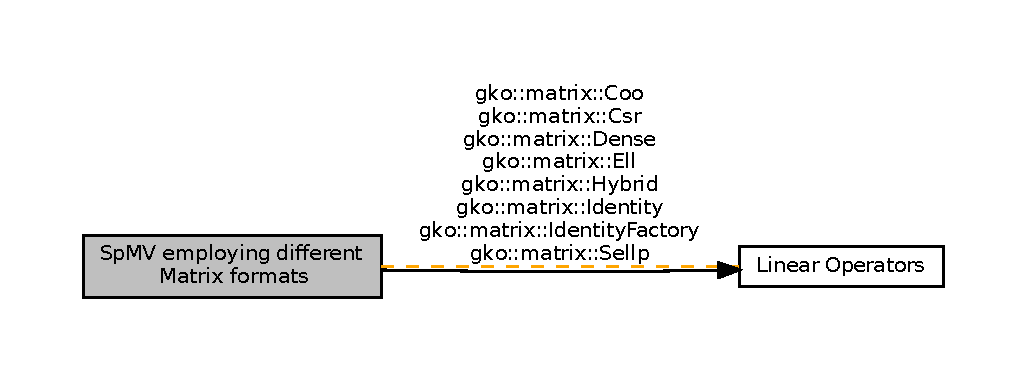
\includegraphics[width=350pt]{group__mat__formats}
\end{center}
\end{figure}
\doxysubsection*{Classes}
\begin{DoxyCompactItemize}
\item 
class \mbox{\hyperlink{classgko_1_1matrix_1_1Coo}{gko\+::matrix\+::\+Coo$<$ Value\+Type, Index\+Type $>$}}
\begin{DoxyCompactList}\small\item\em C\+OO stores a matrix in the coordinate matrix format. \end{DoxyCompactList}\item 
class \mbox{\hyperlink{classgko_1_1matrix_1_1Csr}{gko\+::matrix\+::\+Csr$<$ Value\+Type, Index\+Type $>$}}
\begin{DoxyCompactList}\small\item\em C\+SR is a matrix format which stores only the nonzero coefficients by compressing each row of the matrix (compressed sparse row format). \end{DoxyCompactList}\item 
class \mbox{\hyperlink{classgko_1_1matrix_1_1Dense}{gko\+::matrix\+::\+Dense$<$ Value\+Type $>$}}
\begin{DoxyCompactList}\small\item\em \mbox{\hyperlink{classgko_1_1matrix_1_1Dense}{Dense}} is a matrix format which explicitly stores all values of the matrix. \end{DoxyCompactList}\item 
class \mbox{\hyperlink{classgko_1_1matrix_1_1Diagonal}{gko\+::matrix\+::\+Diagonal$<$ Value\+Type $>$}}
\begin{DoxyCompactList}\small\item\em This class is a utility which efficiently implements the diagonal matrix (a linear operator which scales a vector row wise). \end{DoxyCompactList}\item 
class \mbox{\hyperlink{classgko_1_1matrix_1_1Ell}{gko\+::matrix\+::\+Ell$<$ Value\+Type, Index\+Type $>$}}
\begin{DoxyCompactList}\small\item\em E\+LL is a matrix format where stride with explicit zeros is used such that all rows have the same number of stored elements. \end{DoxyCompactList}\item 
class \mbox{\hyperlink{classgko_1_1matrix_1_1Hybrid}{gko\+::matrix\+::\+Hybrid$<$ Value\+Type, Index\+Type $>$}}
\begin{DoxyCompactList}\small\item\em H\+Y\+B\+R\+ID is a matrix format which splits the matrix into E\+L\+L\+P\+A\+CK and C\+OO format. \end{DoxyCompactList}\item 
class \mbox{\hyperlink{classgko_1_1matrix_1_1Identity}{gko\+::matrix\+::\+Identity$<$ Value\+Type $>$}}
\begin{DoxyCompactList}\small\item\em This class is a utility which efficiently implements the identity matrix (a linear operator which maps each vector to itself). \end{DoxyCompactList}\item 
class \mbox{\hyperlink{classgko_1_1matrix_1_1IdentityFactory}{gko\+::matrix\+::\+Identity\+Factory$<$ Value\+Type $>$}}
\begin{DoxyCompactList}\small\item\em This factory is a utility which can be used to generate \mbox{\hyperlink{classgko_1_1matrix_1_1Identity}{Identity}} operators. \end{DoxyCompactList}\item 
class \mbox{\hyperlink{classgko_1_1matrix_1_1Permutation}{gko\+::matrix\+::\+Permutation$<$ Index\+Type $>$}}
\begin{DoxyCompactList}\small\item\em \mbox{\hyperlink{classgko_1_1matrix_1_1Permutation}{Permutation}} is a matrix \char`\"{}format\char`\"{} which stores the row and column permutation arrays which can be used for re-\/ordering the rows and columns a matrix. \end{DoxyCompactList}\item 
class \mbox{\hyperlink{classgko_1_1matrix_1_1Sellp}{gko\+::matrix\+::\+Sellp$<$ Value\+Type, Index\+Type $>$}}
\begin{DoxyCompactList}\small\item\em S\+E\+L\+L-\/P is a matrix format similar to E\+LL format. \end{DoxyCompactList}\item 
class \mbox{\hyperlink{classgko_1_1matrix_1_1SparsityCsr}{gko\+::matrix\+::\+Sparsity\+Csr$<$ Value\+Type, Index\+Type $>$}}
\begin{DoxyCompactList}\small\item\em \mbox{\hyperlink{classgko_1_1matrix_1_1SparsityCsr}{Sparsity\+Csr}} is a matrix format which stores only the sparsity pattern of a sparse matrix by compressing each row of the matrix (compressed sparse row format). \end{DoxyCompactList}\end{DoxyCompactItemize}
\doxysubsection*{Functions}
\begin{DoxyCompactItemize}
\item 
{\footnotesize template$<$typename Matrix , typename... T\+Args$>$ }\\std\+::unique\+\_\+ptr$<$ Matrix $>$ \mbox{\hyperlink{group__mat__formats_ga2f54bac1e95fb3ef03974fa9c9088491}{gko\+::initialize}} (\mbox{\hyperlink{namespacegko_a6e5c95df0ae4e47aab2f604a22d98ee7}{size\+\_\+type}} stride, std\+::initializer\+\_\+list$<$ typename Matrix\+::value\+\_\+type $>$ vals, std\+::shared\+\_\+ptr$<$ const \mbox{\hyperlink{classgko_1_1Executor}{Executor}} $>$ exec, T\+Args \&\&... create\+\_\+args)
\begin{DoxyCompactList}\small\item\em Creates and initializes a column-\/vector. \end{DoxyCompactList}\item 
{\footnotesize template$<$typename Matrix , typename... T\+Args$>$ }\\std\+::unique\+\_\+ptr$<$ Matrix $>$ \mbox{\hyperlink{group__mat__formats_gaac5f7b4ff3b43dbc6918c687dd7d2d2e}{gko\+::initialize}} (std\+::initializer\+\_\+list$<$ typename Matrix\+::value\+\_\+type $>$ vals, std\+::shared\+\_\+ptr$<$ const \mbox{\hyperlink{classgko_1_1Executor}{Executor}} $>$ exec, T\+Args \&\&... create\+\_\+args)
\begin{DoxyCompactList}\small\item\em Creates and initializes a column-\/vector. \end{DoxyCompactList}\item 
{\footnotesize template$<$typename Matrix , typename... T\+Args$>$ }\\std\+::unique\+\_\+ptr$<$ Matrix $>$ \mbox{\hyperlink{group__mat__formats_gaaf2520e5921e1bea00853c290f4fc28f}{gko\+::initialize}} (\mbox{\hyperlink{namespacegko_a6e5c95df0ae4e47aab2f604a22d98ee7}{size\+\_\+type}} stride, std\+::initializer\+\_\+list$<$ std\+::initializer\+\_\+list$<$ typename Matrix\+::value\+\_\+type $>$$>$ vals, std\+::shared\+\_\+ptr$<$ const \mbox{\hyperlink{classgko_1_1Executor}{Executor}} $>$ exec, T\+Args \&\&... create\+\_\+args)
\begin{DoxyCompactList}\small\item\em Creates and initializes a matrix. \end{DoxyCompactList}\item 
{\footnotesize template$<$typename Matrix , typename... T\+Args$>$ }\\std\+::unique\+\_\+ptr$<$ Matrix $>$ \mbox{\hyperlink{group__mat__formats_gabe4ff67be5b3aae4e981b33ea9883385}{gko\+::initialize}} (std\+::initializer\+\_\+list$<$ std\+::initializer\+\_\+list$<$ typename Matrix\+::value\+\_\+type $>$$>$ vals, std\+::shared\+\_\+ptr$<$ const \mbox{\hyperlink{classgko_1_1Executor}{Executor}} $>$ exec, T\+Args \&\&... create\+\_\+args)
\begin{DoxyCompactList}\small\item\em Creates and initializes a matrix. \end{DoxyCompactList}\end{DoxyCompactItemize}


\doxysubsection{Detailed Description}
A module dedicated to the implementation and usage of the various Matrix Formats in Ginkgo. 



\doxysubsection{Function Documentation}
\mbox{\Hypertarget{group__mat__formats_gaaf2520e5921e1bea00853c290f4fc28f}\label{group__mat__formats_gaaf2520e5921e1bea00853c290f4fc28f}} 
\index{SpMV employing different Matrix formats@{SpMV employing different Matrix formats}!initialize@{initialize}}
\index{initialize@{initialize}!SpMV employing different Matrix formats@{SpMV employing different Matrix formats}}
\doxysubsubsection{\texorpdfstring{initialize()}{initialize()}\hspace{0.1cm}{\footnotesize\ttfamily [1/4]}}
{\footnotesize\ttfamily template$<$typename Matrix , typename... T\+Args$>$ \\
std\+::unique\+\_\+ptr$<$Matrix$>$ gko\+::initialize (\begin{DoxyParamCaption}\item[{\mbox{\hyperlink{namespacegko_a6e5c95df0ae4e47aab2f604a22d98ee7}{size\+\_\+type}}}]{stride,  }\item[{std\+::initializer\+\_\+list$<$ std\+::initializer\+\_\+list$<$ typename Matrix\+::value\+\_\+type $>$$>$}]{vals,  }\item[{std\+::shared\+\_\+ptr$<$ const \mbox{\hyperlink{classgko_1_1Executor}{Executor}} $>$}]{exec,  }\item[{T\+Args \&\&...}]{create\+\_\+args }\end{DoxyParamCaption})}



Creates and initializes a matrix. 

This function first creates a temporary Dense matrix, fills it with passed in values, and then converts the matrix to the requested type.


\begin{DoxyTemplParams}{Template Parameters}
{\em Matrix} & matrix type to initialize (Dense has to implement the Convertible\+To$<$\+Matrix$>$ interface) \\
\hline
{\em T\+Args} & argument types for Matrix\+::create method (not including the implied \mbox{\hyperlink{classgko_1_1Executor}{Executor}} as the first argument)\\
\hline
\end{DoxyTemplParams}

\begin{DoxyParams}{Parameters}
{\em stride} & row stride for the temporary Dense matrix \\
\hline
{\em vals} & values used to initialize the matrix \\
\hline
{\em exec} & \mbox{\hyperlink{classgko_1_1Executor}{Executor}} associated to the matrix \\
\hline
{\em create\+\_\+args} & additional arguments passed to Matrix\+::create, not including the \mbox{\hyperlink{classgko_1_1Executor}{Executor}}, which is passed as the first argument \\
\hline
\end{DoxyParams}


References gko\+::matrix\+::\+Dense$<$ Value\+Type $>$\+::at().

\mbox{\Hypertarget{group__mat__formats_ga2f54bac1e95fb3ef03974fa9c9088491}\label{group__mat__formats_ga2f54bac1e95fb3ef03974fa9c9088491}} 
\index{SpMV employing different Matrix formats@{SpMV employing different Matrix formats}!initialize@{initialize}}
\index{initialize@{initialize}!SpMV employing different Matrix formats@{SpMV employing different Matrix formats}}
\doxysubsubsection{\texorpdfstring{initialize()}{initialize()}\hspace{0.1cm}{\footnotesize\ttfamily [2/4]}}
{\footnotesize\ttfamily template$<$typename Matrix , typename... T\+Args$>$ \\
std\+::unique\+\_\+ptr$<$Matrix$>$ gko\+::initialize (\begin{DoxyParamCaption}\item[{\mbox{\hyperlink{namespacegko_a6e5c95df0ae4e47aab2f604a22d98ee7}{size\+\_\+type}}}]{stride,  }\item[{std\+::initializer\+\_\+list$<$ typename Matrix\+::value\+\_\+type $>$}]{vals,  }\item[{std\+::shared\+\_\+ptr$<$ const \mbox{\hyperlink{classgko_1_1Executor}{Executor}} $>$}]{exec,  }\item[{T\+Args \&\&...}]{create\+\_\+args }\end{DoxyParamCaption})}



Creates and initializes a column-\/vector. 

This function first creates a temporary Dense matrix, fills it with passed in values, and then converts the matrix to the requested type.


\begin{DoxyTemplParams}{Template Parameters}
{\em Matrix} & matrix type to initialize (Dense has to implement the Convertible\+To$<$\+Matrix$>$ interface) \\
\hline
{\em T\+Args} & argument types for Matrix\+::create method (not including the implied \mbox{\hyperlink{classgko_1_1Executor}{Executor}} as the first argument)\\
\hline
\end{DoxyTemplParams}

\begin{DoxyParams}{Parameters}
{\em stride} & row stride for the temporary Dense matrix \\
\hline
{\em vals} & values used to initialize the vector \\
\hline
{\em exec} & \mbox{\hyperlink{classgko_1_1Executor}{Executor}} associated to the vector \\
\hline
{\em create\+\_\+args} & additional arguments passed to Matrix\+::create, not including the \mbox{\hyperlink{classgko_1_1Executor}{Executor}}, which is passed as the first argument \\
\hline
\end{DoxyParams}


References gko\+::matrix\+::\+Dense$<$ Value\+Type $>$\+::at().

\mbox{\Hypertarget{group__mat__formats_gabe4ff67be5b3aae4e981b33ea9883385}\label{group__mat__formats_gabe4ff67be5b3aae4e981b33ea9883385}} 
\index{SpMV employing different Matrix formats@{SpMV employing different Matrix formats}!initialize@{initialize}}
\index{initialize@{initialize}!SpMV employing different Matrix formats@{SpMV employing different Matrix formats}}
\doxysubsubsection{\texorpdfstring{initialize()}{initialize()}\hspace{0.1cm}{\footnotesize\ttfamily [3/4]}}
{\footnotesize\ttfamily template$<$typename Matrix , typename... T\+Args$>$ \\
std\+::unique\+\_\+ptr$<$Matrix$>$ gko\+::initialize (\begin{DoxyParamCaption}\item[{std\+::initializer\+\_\+list$<$ std\+::initializer\+\_\+list$<$ typename Matrix\+::value\+\_\+type $>$$>$}]{vals,  }\item[{std\+::shared\+\_\+ptr$<$ const \mbox{\hyperlink{classgko_1_1Executor}{Executor}} $>$}]{exec,  }\item[{T\+Args \&\&...}]{create\+\_\+args }\end{DoxyParamCaption})}



Creates and initializes a matrix. 

This function first creates a temporary Dense matrix, fills it with passed in values, and then converts the matrix to the requested type. The stride of the intermediate Dense matrix is set to the number of columns of the initializer list.


\begin{DoxyTemplParams}{Template Parameters}
{\em Matrix} & matrix type to initialize (Dense has to implement the Convertible\+To$<$\+Matrix$>$ interface) \\
\hline
{\em T\+Args} & argument types for Matrix\+::create method (not including the implied \mbox{\hyperlink{classgko_1_1Executor}{Executor}} as the first argument)\\
\hline
\end{DoxyTemplParams}

\begin{DoxyParams}{Parameters}
{\em vals} & values used to initialize the matrix \\
\hline
{\em exec} & \mbox{\hyperlink{classgko_1_1Executor}{Executor}} associated to the matrix \\
\hline
{\em create\+\_\+args} & additional arguments passed to Matrix\+::create, not including the \mbox{\hyperlink{classgko_1_1Executor}{Executor}}, which is passed as the first argument \\
\hline
\end{DoxyParams}
\mbox{\Hypertarget{group__mat__formats_gaac5f7b4ff3b43dbc6918c687dd7d2d2e}\label{group__mat__formats_gaac5f7b4ff3b43dbc6918c687dd7d2d2e}} 
\index{SpMV employing different Matrix formats@{SpMV employing different Matrix formats}!initialize@{initialize}}
\index{initialize@{initialize}!SpMV employing different Matrix formats@{SpMV employing different Matrix formats}}
\doxysubsubsection{\texorpdfstring{initialize()}{initialize()}\hspace{0.1cm}{\footnotesize\ttfamily [4/4]}}
{\footnotesize\ttfamily template$<$typename Matrix , typename... T\+Args$>$ \\
std\+::unique\+\_\+ptr$<$Matrix$>$ gko\+::initialize (\begin{DoxyParamCaption}\item[{std\+::initializer\+\_\+list$<$ typename Matrix\+::value\+\_\+type $>$}]{vals,  }\item[{std\+::shared\+\_\+ptr$<$ const \mbox{\hyperlink{classgko_1_1Executor}{Executor}} $>$}]{exec,  }\item[{T\+Args \&\&...}]{create\+\_\+args }\end{DoxyParamCaption})}



Creates and initializes a column-\/vector. 

This function first creates a temporary Dense matrix, fills it with passed in values, and then converts the matrix to the requested type. The stride of the intermediate Dense matrix is set to 1.


\begin{DoxyTemplParams}{Template Parameters}
{\em Matrix} & matrix type to initialize (Dense has to implement the Convertible\+To$<$\+Matrix$>$ interface) \\
\hline
{\em T\+Args} & argument types for Matrix\+::create method (not including the implied \mbox{\hyperlink{classgko_1_1Executor}{Executor}} as the first argument)\\
\hline
\end{DoxyTemplParams}

\begin{DoxyParams}{Parameters}
{\em vals} & values used to initialize the vector \\
\hline
{\em exec} & \mbox{\hyperlink{classgko_1_1Executor}{Executor}} associated to the vector \\
\hline
{\em create\+\_\+args} & additional arguments passed to Matrix\+::create, not including the \mbox{\hyperlink{classgko_1_1Executor}{Executor}}, which is passed as the first argument \\
\hline
\end{DoxyParams}

\hypertarget{group__exec__omp}{}\doxysection{Open\+MP Executor}
\label{group__exec__omp}\index{OpenMP Executor@{OpenMP Executor}}


A module dedicated to the implementation and usage of the Open\+MP executor in Ginkgo.  


Collaboration diagram for Open\+MP Executor\+:
\nopagebreak
\begin{figure}[H]
\begin{center}
\leavevmode
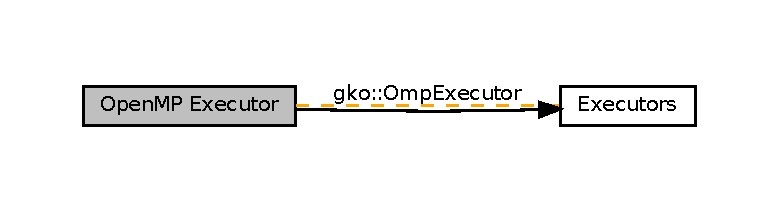
\includegraphics[width=350pt]{group__exec__omp}
\end{center}
\end{figure}
\doxysubsection*{Classes}
\begin{DoxyCompactItemize}
\item 
class \mbox{\hyperlink{classgko_1_1OmpExecutor}{gko\+::\+Omp\+Executor}}
\begin{DoxyCompactList}\small\item\em This is the \mbox{\hyperlink{classgko_1_1Executor}{Executor}} subclass which represents the Open\+MP device (typically C\+PU). \end{DoxyCompactList}\end{DoxyCompactItemize}


\doxysubsection{Detailed Description}
A module dedicated to the implementation and usage of the Open\+MP executor in Ginkgo. 


\hypertarget{group__precond}{}\doxysection{Preconditioners}
\label{group__precond}\index{Preconditioners@{Preconditioners}}


A module dedicated to the implementation and usage of the Preconditioners in Ginkgo.  


Collaboration diagram for Preconditioners\+:
\nopagebreak
\begin{figure}[H]
\begin{center}
\leavevmode
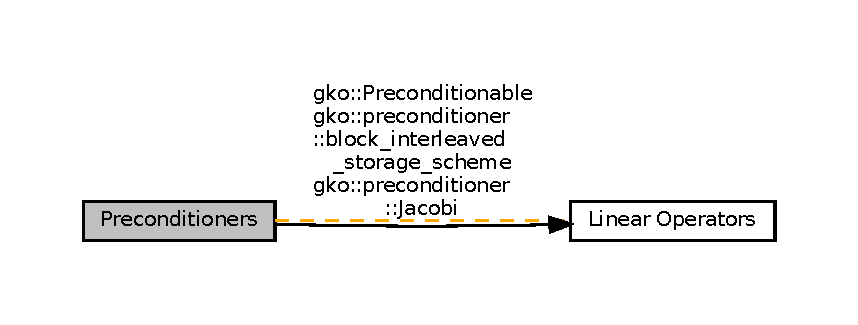
\includegraphics[width=350pt]{group__precond}
\end{center}
\end{figure}
\doxysubsection*{Modules}
\begin{DoxyCompactItemize}
\item 
\mbox{\hyperlink{group__jacobi}{Jacobi Preconditioner}}
\begin{DoxyCompactList}\small\item\em A module dedicated to the implementation and usage of the Jacobi Preconditioner in Ginkgo. \end{DoxyCompactList}\end{DoxyCompactItemize}
\doxysubsection*{Namespaces}
\begin{DoxyCompactItemize}
\item 
 \mbox{\hyperlink{namespacegko_1_1preconditioner}{gko\+::preconditioner}}
\begin{DoxyCompactList}\small\item\em The Preconditioner namespace. \end{DoxyCompactList}\end{DoxyCompactItemize}
\doxysubsection*{Classes}
\begin{DoxyCompactItemize}
\item 
class \mbox{\hyperlink{classgko_1_1Preconditionable}{gko\+::\+Preconditionable}}
\begin{DoxyCompactList}\small\item\em A \mbox{\hyperlink{classgko_1_1LinOp}{Lin\+Op}} implementing this interface can be preconditioned. \end{DoxyCompactList}\item 
class \mbox{\hyperlink{classgko_1_1preconditioner_1_1Ilu}{gko\+::preconditioner\+::\+Ilu$<$ L\+Solver\+Type, U\+Solver\+Type, Reverse\+Apply, Index\+Type $>$}}
\begin{DoxyCompactList}\small\item\em The Incomplete LU (I\+LU) preconditioner solves the equation $LUx = b$ for a given lower triangular matrix L, an upper triangular matrix U and the right hand side b (can contain multiple right hand sides). \end{DoxyCompactList}\item 
class \mbox{\hyperlink{classgko_1_1preconditioner_1_1Jacobi}{gko\+::preconditioner\+::\+Jacobi$<$ Value\+Type, Index\+Type $>$}}
\begin{DoxyCompactList}\small\item\em A block-\/\+Jacobi preconditioner is a block-\/diagonal linear operator, obtained by inverting the diagonal blocks of the source operator. \end{DoxyCompactList}\end{DoxyCompactItemize}


\doxysubsection{Detailed Description}
A module dedicated to the implementation and usage of the Preconditioners in Ginkgo. 


\hypertarget{group__exec__ref}{}\doxysection{Reference Executor}
\label{group__exec__ref}\index{Reference Executor@{Reference Executor}}


A module dedicated to the implementation and usage of the Reference executor in Ginkgo.  


Collaboration diagram for Reference Executor\+:
\nopagebreak
\begin{figure}[H]
\begin{center}
\leavevmode
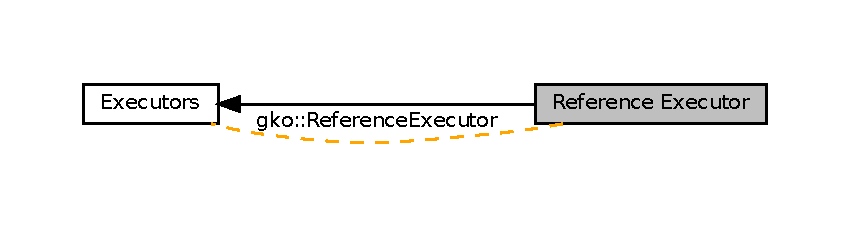
\includegraphics[width=350pt]{group__exec__ref}
\end{center}
\end{figure}
\doxysubsection*{Classes}
\begin{DoxyCompactItemize}
\item 
class \mbox{\hyperlink{classgko_1_1ReferenceExecutor}{gko\+::\+Reference\+Executor}}
\begin{DoxyCompactList}\small\item\em This is a specialization of the \mbox{\hyperlink{classgko_1_1OmpExecutor}{Omp\+Executor}}, which runs the reference implementations of the kernels used for debugging purposes. \end{DoxyCompactList}\end{DoxyCompactItemize}


\doxysubsection{Detailed Description}
A module dedicated to the implementation and usage of the Reference executor in Ginkgo. 


\hypertarget{group__solvers}{}\doxysection{Solvers}
\label{group__solvers}\index{Solvers@{Solvers}}


A module dedicated to the implementation and usage of the Solvers in Ginkgo.  


Collaboration diagram for Solvers\+:
\nopagebreak
\begin{figure}[H]
\begin{center}
\leavevmode
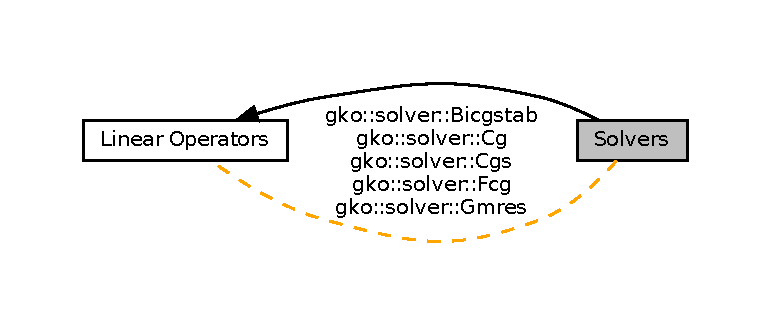
\includegraphics[width=350pt]{group__solvers}
\end{center}
\end{figure}
\doxysubsection*{Namespaces}
\begin{DoxyCompactItemize}
\item 
 \mbox{\hyperlink{namespacegko_1_1solver}{gko\+::solver}}
\begin{DoxyCompactList}\small\item\em The ginkgo Solve namespace. \end{DoxyCompactList}\end{DoxyCompactItemize}
\doxysubsection*{Classes}
\begin{DoxyCompactItemize}
\item 
class \mbox{\hyperlink{classgko_1_1solver_1_1Bicgstab}{gko\+::solver\+::\+Bicgstab$<$ Value\+Type $>$}}
\begin{DoxyCompactList}\small\item\em Bi\+C\+G\+S\+T\+AB or the Bi-\/\+Conjugate Gradient-\/\+Stabilized is a Krylov subspace solver. \end{DoxyCompactList}\item 
class \mbox{\hyperlink{classgko_1_1solver_1_1Cg}{gko\+::solver\+::\+Cg$<$ Value\+Type $>$}}
\begin{DoxyCompactList}\small\item\em CG or the conjugate gradient method is an iterative type Krylov subspace method which is suitable for symmetric positive definite methods. \end{DoxyCompactList}\item 
class \mbox{\hyperlink{classgko_1_1solver_1_1Cgs}{gko\+::solver\+::\+Cgs$<$ Value\+Type $>$}}
\begin{DoxyCompactList}\small\item\em C\+GS or the conjugate gradient square method is an iterative type Krylov subspace method which is suitable for general systems. \end{DoxyCompactList}\item 
class \mbox{\hyperlink{classgko_1_1solver_1_1Fcg}{gko\+::solver\+::\+Fcg$<$ Value\+Type $>$}}
\begin{DoxyCompactList}\small\item\em F\+CG or the flexible conjugate gradient method is an iterative type Krylov subspace method which is suitable for symmetric positive definite methods. \end{DoxyCompactList}\item 
class \mbox{\hyperlink{classgko_1_1solver_1_1Gmres}{gko\+::solver\+::\+Gmres$<$ Value\+Type $>$}}
\begin{DoxyCompactList}\small\item\em G\+M\+R\+ES or the generalized minimal residual method is an iterative type Krylov subspace method which is suitable for nonsymmetric linear systems. \end{DoxyCompactList}\item 
class \mbox{\hyperlink{classgko_1_1solver_1_1LowerTrs}{gko\+::solver\+::\+Lower\+Trs$<$ Value\+Type, Index\+Type $>$}}
\begin{DoxyCompactList}\small\item\em \mbox{\hyperlink{classgko_1_1solver_1_1LowerTrs}{Lower\+Trs}} is the triangular solver which solves the system L x = b, when L is a lower triangular matrix. \end{DoxyCompactList}\item 
class \mbox{\hyperlink{classgko_1_1solver_1_1UpperTrs}{gko\+::solver\+::\+Upper\+Trs$<$ Value\+Type, Index\+Type $>$}}
\begin{DoxyCompactList}\small\item\em \mbox{\hyperlink{classgko_1_1solver_1_1UpperTrs}{Upper\+Trs}} is the triangular solver which solves the system U x = b, when U is an upper triangular matrix. \end{DoxyCompactList}\end{DoxyCompactItemize}


\doxysubsection{Detailed Description}
A module dedicated to the implementation and usage of the Solvers in Ginkgo. 


\hypertarget{group__stop}{}\section{Stopping criteria}
\label{group__stop}\index{Stopping criteria@{Stopping criteria}}


A module dedicated to the implementation and usage of the Stopping Criteria in Ginkgo.  


\subsection*{Namespaces}
\begin{DoxyCompactItemize}
\item 
 \hyperlink{namespacegko_1_1stop}{gko\+::stop}
\begin{DoxyCompactList}\small\item\em The Stopping criterion namespace. \end{DoxyCompactList}\end{DoxyCompactItemize}
\subsection*{Classes}
\begin{DoxyCompactItemize}
\item 
class \hyperlink{classgko_1_1stop_1_1Combined}{gko\+::stop\+::\+Combined}
\begin{DoxyCompactList}\small\item\em The \hyperlink{classgko_1_1stop_1_1Combined}{Combined} class is used to combine multiple criterions together through an OR operation. \end{DoxyCompactList}\item 
class \hyperlink{classgko_1_1stop_1_1Iteration}{gko\+::stop\+::\+Iteration}
\begin{DoxyCompactList}\small\item\em The \hyperlink{classgko_1_1stop_1_1Iteration}{Iteration} class is a stopping criterion which stops the iteration process after a preset number of iterations. \end{DoxyCompactList}\item 
class \hyperlink{classgko_1_1stop_1_1ResidualNormReduction}{gko\+::stop\+::\+Residual\+Norm\+Reduction$<$ Value\+Type $>$}
\begin{DoxyCompactList}\small\item\em The \hyperlink{classgko_1_1stop_1_1ResidualNormReduction}{Residual\+Norm\+Reduction} class is a stopping criterion which stops the iteration process when the relative residual norm is below a certain threshold. \end{DoxyCompactList}\item 
class \hyperlink{classgko_1_1stopping__status}{gko\+::stopping\+\_\+status}
\begin{DoxyCompactList}\small\item\em This class is used to keep track of the stopping status of one vector. \end{DoxyCompactList}\item 
class \hyperlink{classgko_1_1stop_1_1Time}{gko\+::stop\+::\+Time}
\begin{DoxyCompactList}\small\item\em The \hyperlink{classgko_1_1stop_1_1Time}{Time} class is a stopping criterion which stops the iteration process after a certain amout of time has passed. \end{DoxyCompactList}\end{DoxyCompactItemize}
\subsection*{Macros}
\begin{DoxyCompactItemize}
\item 
\#define \hyperlink{group__stop_ga5a998013602bad749e586a5664670cae}{G\+K\+O\+\_\+\+E\+N\+A\+B\+L\+E\+\_\+\+C\+R\+I\+T\+E\+R\+I\+O\+N\+\_\+\+F\+A\+C\+T\+O\+RY}(\+\_\+criterion,  \+\_\+parameters\+\_\+name,  \+\_\+factory\+\_\+name)
\begin{DoxyCompactList}\small\item\em This macro will generate a default implementation of a Criterion\+Factory for the Criterion subclass it is defined in. \end{DoxyCompactList}\end{DoxyCompactItemize}
\subsection*{Functions}
\begin{DoxyCompactItemize}
\item 
{\footnotesize template$<$typename Factory\+Container $>$ }\\std\+::shared\+\_\+ptr$<$ const \hyperlink{namespacegko_1_1stop_ab12a51109c50b35ec36dc5a393d6a9a0}{Criterion\+Factory} $>$ \hyperlink{group__stop_ga3a3325b3a7660501f3bb72d08b09f2d2}{gko\+::stop\+::combine} (Factory\+Container \&\&factories)
\begin{DoxyCompactList}\small\item\em Combines multiple criterion factories into a single combined criterion factory. \end{DoxyCompactList}\end{DoxyCompactItemize}


\subsection{Detailed Description}
A module dedicated to the implementation and usage of the Stopping Criteria in Ginkgo. 



\subsection{Macro Definition Documentation}
\mbox{\Hypertarget{group__stop_ga5a998013602bad749e586a5664670cae}\label{group__stop_ga5a998013602bad749e586a5664670cae}} 
\index{Stopping criteria@{Stopping criteria}!G\+K\+O\+\_\+\+E\+N\+A\+B\+L\+E\+\_\+\+C\+R\+I\+T\+E\+R\+I\+O\+N\+\_\+\+F\+A\+C\+T\+O\+RY@{G\+K\+O\+\_\+\+E\+N\+A\+B\+L\+E\+\_\+\+C\+R\+I\+T\+E\+R\+I\+O\+N\+\_\+\+F\+A\+C\+T\+O\+RY}}
\index{G\+K\+O\+\_\+\+E\+N\+A\+B\+L\+E\+\_\+\+C\+R\+I\+T\+E\+R\+I\+O\+N\+\_\+\+F\+A\+C\+T\+O\+RY@{G\+K\+O\+\_\+\+E\+N\+A\+B\+L\+E\+\_\+\+C\+R\+I\+T\+E\+R\+I\+O\+N\+\_\+\+F\+A\+C\+T\+O\+RY}!Stopping criteria@{Stopping criteria}}
\subsubsection{\texorpdfstring{G\+K\+O\+\_\+\+E\+N\+A\+B\+L\+E\+\_\+\+C\+R\+I\+T\+E\+R\+I\+O\+N\+\_\+\+F\+A\+C\+T\+O\+RY}{GKO\_ENABLE\_CRITERION\_FACTORY}}
{\footnotesize\ttfamily \#define G\+K\+O\+\_\+\+E\+N\+A\+B\+L\+E\+\_\+\+C\+R\+I\+T\+E\+R\+I\+O\+N\+\_\+\+F\+A\+C\+T\+O\+RY(\begin{DoxyParamCaption}\item[{}]{\+\_\+criterion,  }\item[{}]{\+\_\+parameters\+\_\+name,  }\item[{}]{\+\_\+factory\+\_\+name }\end{DoxyParamCaption})}

{\bfseries Value\+:}
\begin{DoxyCode}
\textcolor{keyword}{public}:                                                                      \(\backslash\)
    const \_parameters\_name##\_type &get\_##\_parameters\_name() const            \(\backslash\)
    \{                                                                        \(\backslash\)
        return \_parameters\_name##\_;                                          \(\backslash\)
    \}                                                                        \(\backslash\)
                                                                             \(\backslash\)
    class \_factory\_name                                                      \(\backslash\)
        : public ::gko::stop::EnableDefaultCriterionFactory<                 \(\backslash\)
              \_factory\_name, \_criterion, \_parameters\_name##\_type> \{          \(\backslash\)
        friend class ::gko::EnablePolymorphicObject<                         \(\backslash\)
            \_factory\_name, \hyperlink{classgko_1_1AbstractFactory}{::gko::stop::CriterionFactory}>;                   \(\backslash\)
        friend class ::gko::enable\_parameters\_type<\_parameters\_name##\_type,  \(\backslash\)
                                                   \_factory\_name>;           \(\backslash\)
        using ::gko::stop::EnableDefaultCriterionFactory<                    \(\backslash\)
            \_factory\_name, \_criterion,                                       \(\backslash\)
            \_parameters\_name##\_type>::EnableDefaultCriterionFactory;         \(\backslash\)
    \};                                                                       \(\backslash\)
    friend ::gko::stop::EnableDefaultCriterionFactory<                       \(\backslash\)
        \_factory\_name, \_criterion, \_parameters\_name##\_type>;                 \(\backslash\)
                                                                             \(\backslash\)
private:                                                                     \(\backslash\)
    \_parameters\_name##\_type \_parameters\_name##\_;                             \(\backslash\)
                                                                             \(\backslash\)
public:                                                                      \(\backslash\)
    static\_assert(\textcolor{keyword}{true},                                                      \(\backslash\)
                  \textcolor{stringliteral}{"This assert is used to counter the false positive extra "} \(\backslash\)
                  \textcolor{stringliteral}{"semi-colon warnings"})
\end{DoxyCode}


This macro will generate a default implementation of a Criterion\+Factory for the Criterion subclass it is defined in. 

This macro is very similar to the macro \#\+E\+N\+A\+B\+L\+E\+\_\+\+L\+I\+N\+\_\+\+O\+P\+\_\+\+F\+A\+C\+T\+O\+R\+Y(). A more detailed description of the use of these type of macros can be found there.


\begin{DoxyParams}{Parameters}
{\em \+\_\+criterion} & concrete operator for which the factory is to be created \mbox{[}C\+R\+TP parameter\mbox{]} \\
\hline
{\em \+\_\+parameters\+\_\+name} & name of the parameters member in the class (its type is {\ttfamily $<$\+\_\+parameters\+\_\+name$>$\+\_\+type}, the protected member\textquotesingle{}s name is {\ttfamily $<$\+\_\+parameters\+\_\+name$>$\+\_\+}, and the public getter\textquotesingle{}s name is {\ttfamily get\+\_\+$<$\+\_\+parameters\+\_\+name$>$()}) \\
\hline
{\em \+\_\+factory\+\_\+name} & name of the generated factory type \\
\hline
\end{DoxyParams}


\subsection{Function Documentation}
\mbox{\Hypertarget{group__stop_ga3a3325b3a7660501f3bb72d08b09f2d2}\label{group__stop_ga3a3325b3a7660501f3bb72d08b09f2d2}} 
\index{Stopping criteria@{Stopping criteria}!combine@{combine}}
\index{combine@{combine}!Stopping criteria@{Stopping criteria}}
\subsubsection{\texorpdfstring{combine()}{combine()}}
{\footnotesize\ttfamily template$<$typename Factory\+Container $>$ \\
std\+::shared\+\_\+ptr$<$const \hyperlink{namespacegko_1_1stop_ab12a51109c50b35ec36dc5a393d6a9a0}{Criterion\+Factory}$>$ gko\+::stop\+::combine (\begin{DoxyParamCaption}\item[{Factory\+Container \&\&}]{factories }\end{DoxyParamCaption})}



Combines multiple criterion factories into a single combined criterion factory. 

This function treats a singleton container as a special case and avoids creating an additional object and just returns the input factory.


\begin{DoxyTemplParams}{Template Parameters}
{\em Factory\+Container} & a random access container type\\
\hline
\end{DoxyTemplParams}

\begin{DoxyParams}{Parameters}
{\em factories} & a list of factories to combined\\
\hline
\end{DoxyParams}
\begin{DoxyReturn}{Returns}
a combined criterion factory if the input contains multiple factories or the input factory if the input contains only one factory 
\end{DoxyReturn}

\hypertarget{group__linop__class}{}\section{Linop\+\_\+class}
\label{group__linop__class}\index{Linop\+\_\+class@{Linop\+\_\+class}}


The linear operator (\hyperlink{classgko_1_1LinOp}{Lin\+Op}) is a base class for all linear algebra objects in Ginkgo.  


Collaboration diagram for Linop\+\_\+class\+:
\nopagebreak
\begin{figure}[H]
\begin{center}
\leavevmode
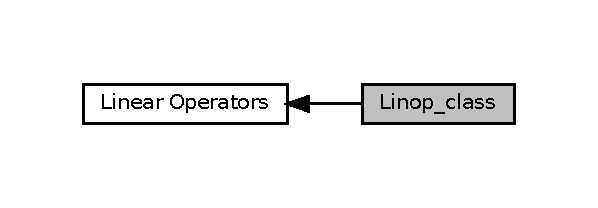
\includegraphics[width=287pt]{group__linop__class}
\end{center}
\end{figure}
The linear operator (\hyperlink{classgko_1_1LinOp}{Lin\+Op}) is a base class for all linear algebra objects in Ginkgo. 

The main benefit of having a single base class for the entire collection of linear algebra objects (as opposed to having separate hierarchies for matrices, solvers and preconditioners) is the generality it provides.

First, since all subclasses provide a common interface, the library users are exposed to a smaller set of routines. For example, a matrix-\/vector product, a preconditioner application, or even a system solve are just different terms given to the operation of applying a certain linear operator to a vector. As such, Ginkgo uses the same routine name, \hyperlink{classgko_1_1LinOp_a0449b2fc705d2f970855af23b5e2788e}{Lin\+Op\+::apply()} for each of these operations, where the actual operation performed depends on the type of linear operator involved in the operation.

Second, a common interface often allows for writing more generic code. If a user\textquotesingle{}s routine requires only operations provided by the \hyperlink{classgko_1_1LinOp}{Lin\+Op} interface, the same code can be used for any kind of linear operators, independent of whether these are matrices, solvers or preconditioners. This feature is also extensively used in Ginkgo itself. For example, a preconditioner used inside a Krylov solver is a \hyperlink{classgko_1_1LinOp}{Lin\+Op}. This allows the user to supply a wide variety of preconditioners\+: either the ones which were designed to be used in this scenario (like I\+LU or block-\/\+Jacobi), a user-\/supplied matrix which is known to be a good preconditioner for the specific problem, or even another solver (e.\+g., if constructing a flexible G\+M\+R\+ES solver).

A key observation for providing a unified interface for matrices, solvers, and preconditioners is that the most common operation performed on all of them can be expressed as an application of a linear operator to a vector\+:


\begin{DoxyItemize}
\item the sparse matrix-\/vector product with a matrix $A$ is a linear operator application $y = Ax$;
\item the application of a preconditioner is a linear operator application $y = M^{-1}x$, where $M$ is an approximation of the original system matrix $A$ (thus a preconditioner represents an \char`\"{}approximate
    inverse\char`\"{} operator $M^{-1}$).
\item the system solve $Ax = b$ can be viewed as linear operator application $x = A^{-1}b$ (it goes without saying that the implementation of linear system solves does not follow this conceptual idea), so a linear system solver can be viewed as a representation of the operator $A^{-1}$.
\end{DoxyItemize}

Finally, direct manipulation of \hyperlink{classgko_1_1LinOp}{Lin\+Op} objects is rarely required in simple scenarios. As an illustrative example, one could construct a fixed-\/point iteration routine $x_{k+1} = Lx_k + b$ as follows\+:


\begin{DoxyCode}
std::unique\_ptr<matrix::Dense<>> calculate\_fixed\_point(
        \textcolor{keywordtype}{int} iters, \textcolor{keyword}{const} LinOp *L, \textcolor{keyword}{const} matrix::Dense<> *x0
        \textcolor{keyword}{const} matrix::Dense<> *b)
\{
    \textcolor{keyword}{auto} x = gko::clone(x0);
    \textcolor{keyword}{auto} tmp = gko::clone(x0);
    \textcolor{keyword}{auto} \hyperlink{namespacegko_a0059e27f8f4bc348ff65c1e60caf47c8}{one} = Dense<>::create(L->get\_executor(), \{1.0,\});
    \textcolor{keywordflow}{for} (\textcolor{keywordtype}{int} i = 0; i < iters; ++i) \{
        L->apply(gko::lend(tmp), gko::lend(x));
        x->add\_scaled(gko::lend(\hyperlink{namespacegko_a0059e27f8f4bc348ff65c1e60caf47c8}{one}), gko::lend(b));
        tmp->copy\_from(gko::lend(x));
    \}
    \textcolor{keywordflow}{return} x;
\}
\end{DoxyCode}


Here, if $L$ is a matrix, \hyperlink{classgko_1_1LinOp_a0449b2fc705d2f970855af23b5e2788e}{Lin\+Op\+::apply()} refers to the matrix vector product, and {\ttfamily L-\/$>$apply(a, b)} computes $b = L \cdot a$. {\ttfamily x-\/$>$add\+\_\+scaled(one.\+get(), b.\+get())} is the {\ttfamily axpy} vector update $x:=x+b$.

The interesting part of this example is the apply() routine at line 4 of the function body. Since this routine is part of the \hyperlink{classgko_1_1LinOp}{Lin\+Op} base class, the fixed-\/point iteration routine can calculate a fixed point not only for matrices, but for any type of linear operator. 
\hypertarget{group__logger__class}{}\section{Logger\+\_\+class}
\label{group__logger__class}\index{Logger\+\_\+class@{Logger\+\_\+class}}


The \hyperlink{classgko_1_1log_1_1Logger}{Logger} class represents a simple \hyperlink{classgko_1_1log_1_1Logger}{Logger} object.  


The \hyperlink{classgko_1_1log_1_1Logger}{Logger} class represents a simple \hyperlink{classgko_1_1log_1_1Logger}{Logger} object. 

It comprises all masks and events internally. Every new logging event addition should be done here. The \hyperlink{classgko_1_1log_1_1Logger}{Logger} class also provides a default implementation for most events which do nothing, therefore it is not an obligation to change all classes which derive from \hyperlink{classgko_1_1log_1_1Logger}{Logger}, although it is good practice. The logger class is built using event masks to control which events should be logged, and which should not. 
\chapter{Namespace Documentation}
\hypertarget{namespacegko}{}\doxysection{gko Namespace Reference}
\label{namespacegko}\index{gko@{gko}}


The Ginkgo namespace.  


\doxysubsection*{Namespaces}
\begin{DoxyCompactItemize}
\item 
 \mbox{\hyperlink{namespacegko_1_1accessor}{accessor}}
\begin{DoxyCompactList}\small\item\em The accessor namespace. \end{DoxyCompactList}\item 
 \mbox{\hyperlink{namespacegko_1_1factorization}{factorization}}
\begin{DoxyCompactList}\small\item\em The Factorization namespace. \end{DoxyCompactList}\item 
 \mbox{\hyperlink{namespacegko_1_1log}{log}}
\begin{DoxyCompactList}\small\item\em The logger namespace . \end{DoxyCompactList}\item 
 \mbox{\hyperlink{namespacegko_1_1matrix}{matrix}}
\begin{DoxyCompactList}\small\item\em The matrix namespace. \end{DoxyCompactList}\item 
 \mbox{\hyperlink{namespacegko_1_1name__demangling}{name\+\_\+demangling}}
\begin{DoxyCompactList}\small\item\em The name demangling namespace. \end{DoxyCompactList}\item 
 \mbox{\hyperlink{namespacegko_1_1preconditioner}{preconditioner}}
\begin{DoxyCompactList}\small\item\em The Preconditioner namespace. \end{DoxyCompactList}\item 
 \mbox{\hyperlink{namespacegko_1_1reorder}{reorder}}
\begin{DoxyCompactList}\small\item\em The Reorder namespace. \end{DoxyCompactList}\item 
 \mbox{\hyperlink{namespacegko_1_1solver}{solver}}
\begin{DoxyCompactList}\small\item\em The ginkgo Solve namespace. \end{DoxyCompactList}\item 
 \mbox{\hyperlink{namespacegko_1_1stop}{stop}}
\begin{DoxyCompactList}\small\item\em The Stopping criterion namespace. \end{DoxyCompactList}\item 
 \mbox{\hyperlink{namespacegko_1_1syn}{syn}}
\begin{DoxyCompactList}\small\item\em The Synthesizer namespace. \end{DoxyCompactList}\item 
 \mbox{\hyperlink{namespacegko_1_1xstd}{xstd}}
\begin{DoxyCompactList}\small\item\em The namespace for functionalities after C++14 standard. \end{DoxyCompactList}\end{DoxyCompactItemize}
\doxysubsection*{Classes}
\begin{DoxyCompactItemize}
\item 
class \mbox{\hyperlink{classgko_1_1AbsoluteComputable}{Absolute\+Computable}}
\begin{DoxyCompactList}\small\item\em The \mbox{\hyperlink{classgko_1_1AbsoluteComputable}{Absolute\+Computable}} is an interface that allows to get the component wise absolute of a \mbox{\hyperlink{classgko_1_1LinOp}{Lin\+Op}}. \end{DoxyCompactList}\item 
class \mbox{\hyperlink{classgko_1_1AbstractFactory}{Abstract\+Factory}}
\begin{DoxyCompactList}\small\item\em The \mbox{\hyperlink{classgko_1_1AbstractFactory}{Abstract\+Factory}} is a generic interface template that enables easy implementation of the abstract factory design pattern. \end{DoxyCompactList}\item 
class \mbox{\hyperlink{classgko_1_1AllocationError}{Allocation\+Error}}
\begin{DoxyCompactList}\small\item\em \mbox{\hyperlink{classgko_1_1AllocationError}{Allocation\+Error}} is thrown if a memory allocation fails. \end{DoxyCompactList}\item 
class \mbox{\hyperlink{classgko_1_1Array}{Array}}
\begin{DoxyCompactList}\small\item\em An \mbox{\hyperlink{classgko_1_1Array}{Array}} is a container which encapsulates fixed-\/sized arrays, stored on the \mbox{\hyperlink{classgko_1_1Executor}{Executor}} tied to the \mbox{\hyperlink{classgko_1_1Array}{Array}}. \end{DoxyCompactList}\item 
class \mbox{\hyperlink{classgko_1_1BadDimension}{Bad\+Dimension}}
\begin{DoxyCompactList}\small\item\em \mbox{\hyperlink{classgko_1_1BadDimension}{Bad\+Dimension}} is thrown if an operation is being applied to a \mbox{\hyperlink{classgko_1_1LinOp}{Lin\+Op}} with bad dimensions. \end{DoxyCompactList}\item 
class \mbox{\hyperlink{classgko_1_1Combination}{Combination}}
\begin{DoxyCompactList}\small\item\em The \mbox{\hyperlink{classgko_1_1Combination}{Combination}} class can be used to construct a linear combination of multiple linear operators {\ttfamily c1 $\ast$ op1 + c2 $\ast$ op2 + ... }\end{DoxyCompactList}\item 
class \mbox{\hyperlink{classgko_1_1Composition}{Composition}}
\begin{DoxyCompactList}\small\item\em The \mbox{\hyperlink{classgko_1_1Composition}{Composition}} class can be used to compose linear operators {\ttfamily op1, op2, ..., opn} and obtain the operator {\ttfamily op1 $\ast$ op2 $\ast$ ... }\end{DoxyCompactList}\item 
class \mbox{\hyperlink{classgko_1_1ConvertibleTo}{Convertible\+To}}
\begin{DoxyCompactList}\small\item\em \mbox{\hyperlink{classgko_1_1ConvertibleTo}{Convertible\+To}} interface is used to mark that the implementer can be converted to the object of Result\+Type. \end{DoxyCompactList}\item 
class \mbox{\hyperlink{classgko_1_1copy__back__deleter}{copy\+\_\+back\+\_\+deleter}}
\begin{DoxyCompactList}\small\item\em A \mbox{\hyperlink{classgko_1_1copy__back__deleter}{copy\+\_\+back\+\_\+deleter}} is a type of deleter that copies the data to an internally referenced object before performing the deletion. \end{DoxyCompactList}\item 
class \mbox{\hyperlink{classgko_1_1copy__back__deleter_3_01const_01T_01_4}{copy\+\_\+back\+\_\+deleter$<$ const T $>$}}
\item 
struct \mbox{\hyperlink{structgko_1_1cpx__real__type}{cpx\+\_\+real\+\_\+type}}
\begin{DoxyCompactList}\small\item\em Access the underlying real type of a complex number. \end{DoxyCompactList}\item 
struct {\bfseries cpx\+\_\+real\+\_\+type$<$ std\+::complex$<$ T $>$ $>$}
\begin{DoxyCompactList}\small\item\em Specialization for complex types. \end{DoxyCompactList}\item 
class \mbox{\hyperlink{classgko_1_1CublasError}{Cublas\+Error}}
\begin{DoxyCompactList}\small\item\em \mbox{\hyperlink{classgko_1_1CublasError}{Cublas\+Error}} is thrown when a cu\+B\+L\+AS routine throws a non-\/zero error code. \end{DoxyCompactList}\item 
class \mbox{\hyperlink{classgko_1_1CudaError}{Cuda\+Error}}
\begin{DoxyCompactList}\small\item\em \mbox{\hyperlink{classgko_1_1CudaError}{Cuda\+Error}} is thrown when a C\+U\+DA routine throws a non-\/zero error code. \end{DoxyCompactList}\item 
class \mbox{\hyperlink{classgko_1_1CudaExecutor}{Cuda\+Executor}}
\begin{DoxyCompactList}\small\item\em This is the \mbox{\hyperlink{classgko_1_1Executor}{Executor}} subclass which represents the C\+U\+DA device. \end{DoxyCompactList}\item 
class \mbox{\hyperlink{classgko_1_1CusparseError}{Cusparse\+Error}}
\begin{DoxyCompactList}\small\item\em \mbox{\hyperlink{classgko_1_1CusparseError}{Cusparse\+Error}} is thrown when a cu\+S\+P\+A\+R\+SE routine throws a non-\/zero error code. \end{DoxyCompactList}\item 
struct \mbox{\hyperlink{structgko_1_1default__converter}{default\+\_\+converter}}
\begin{DoxyCompactList}\small\item\em Used to convert objects of type {\ttfamily S} to objects of type {\ttfamily R} using static\+\_\+cast. \end{DoxyCompactList}\item 
class \mbox{\hyperlink{classgko_1_1DiagonalExtractable}{Diagonal\+Extractable}}
\begin{DoxyCompactList}\small\item\em The diagonal of a \mbox{\hyperlink{classgko_1_1LinOp}{Lin\+Op}} implementing this interface can be extracted. \end{DoxyCompactList}\item 
struct \mbox{\hyperlink{structgko_1_1dim}{dim}}
\begin{DoxyCompactList}\small\item\em A type representing the dimensions of a multidimensional object. \end{DoxyCompactList}\item 
struct \mbox{\hyperlink{structgko_1_1dim_3_011u_00_01DimensionType_01_4}{dim$<$ 1u, Dimension\+Type $>$}}
\item 
class \mbox{\hyperlink{classgko_1_1DimensionMismatch}{Dimension\+Mismatch}}
\begin{DoxyCompactList}\small\item\em \mbox{\hyperlink{classgko_1_1DimensionMismatch}{Dimension\+Mismatch}} is thrown if an operation is being applied to Lin\+Ops of incompatible size. \end{DoxyCompactList}\item 
struct \mbox{\hyperlink{structgko_1_1enable__parameters__type}{enable\+\_\+parameters\+\_\+type}}
\begin{DoxyCompactList}\small\item\em The \mbox{\hyperlink{structgko_1_1enable__parameters__type}{enable\+\_\+parameters\+\_\+type}} mixin is used to create a base implementation of the factory parameters structure. \end{DoxyCompactList}\item 
class \mbox{\hyperlink{classgko_1_1EnableAbsoluteComputation}{Enable\+Absolute\+Computation}}
\begin{DoxyCompactList}\small\item\em The \mbox{\hyperlink{classgko_1_1EnableAbsoluteComputation}{Enable\+Absolute\+Computation}} mixin provides the default implementations of {\ttfamily compute\+\_\+absolute\+\_\+linop} and the absolute interface. \end{DoxyCompactList}\item 
class \mbox{\hyperlink{classgko_1_1EnableAbstractPolymorphicObject}{Enable\+Abstract\+Polymorphic\+Object}}
\begin{DoxyCompactList}\small\item\em This mixin inherits from (a subclass of) \mbox{\hyperlink{classgko_1_1PolymorphicObject}{Polymorphic\+Object}} and provides a base implementation of a new abstract object. \end{DoxyCompactList}\item 
class \mbox{\hyperlink{classgko_1_1EnableCreateMethod}{Enable\+Create\+Method}}
\begin{DoxyCompactList}\small\item\em This mixin implements a static {\ttfamily create()} method on {\ttfamily Concrete\+Type} that dynamically allocates the memory, uses the passed-\/in arguments to construct the object, and returns an std\+::unique\+\_\+ptr to such an object. \end{DoxyCompactList}\item 
class \mbox{\hyperlink{classgko_1_1EnableDefaultFactory}{Enable\+Default\+Factory}}
\begin{DoxyCompactList}\small\item\em This mixin provides a default implementation of a concrete factory. \end{DoxyCompactList}\item 
class \mbox{\hyperlink{classgko_1_1EnableLinOp}{Enable\+Lin\+Op}}
\begin{DoxyCompactList}\small\item\em The \mbox{\hyperlink{classgko_1_1EnableLinOp}{Enable\+Lin\+Op}} mixin can be used to provide sensible default implementations of the majority of the \mbox{\hyperlink{classgko_1_1LinOp}{Lin\+Op}} and \mbox{\hyperlink{classgko_1_1PolymorphicObject}{Polymorphic\+Object}} interface. \end{DoxyCompactList}\item 
class \mbox{\hyperlink{classgko_1_1EnablePolymorphicAssignment}{Enable\+Polymorphic\+Assignment}}
\begin{DoxyCompactList}\small\item\em This mixin is used to enable a default \mbox{\hyperlink{classgko_1_1PolymorphicObject_a5e6f713938293cfbe788d00480eb4d81}{Polymorphic\+Object\+::copy\+\_\+from()}} implementation for objects that have implemented conversions between them. \end{DoxyCompactList}\item 
class \mbox{\hyperlink{classgko_1_1EnablePolymorphicObject}{Enable\+Polymorphic\+Object}}
\begin{DoxyCompactList}\small\item\em This mixin inherits from (a subclass of) \mbox{\hyperlink{classgko_1_1PolymorphicObject}{Polymorphic\+Object}} and provides a base implementation of a new concrete polymorphic object. \end{DoxyCompactList}\item 
class \mbox{\hyperlink{classgko_1_1Error}{Error}}
\begin{DoxyCompactList}\small\item\em The \mbox{\hyperlink{classgko_1_1Error}{Error}} class is used to report exceptional behaviour in library functions. \end{DoxyCompactList}\item 
class \mbox{\hyperlink{classgko_1_1Executor}{Executor}}
\begin{DoxyCompactList}\small\item\em The first step in using the Ginkgo library consists of creating an executor. \end{DoxyCompactList}\item 
class \mbox{\hyperlink{classgko_1_1executor__deleter}{executor\+\_\+deleter}}
\begin{DoxyCompactList}\small\item\em This is a deleter that uses an executor\textquotesingle{}s {\ttfamily free} method to deallocate the data. \end{DoxyCompactList}\item 
class \mbox{\hyperlink{classgko_1_1executor__deleter_3_01T_0f_0e_4}{executor\+\_\+deleter$<$ T\mbox{[}$\,$\mbox{]}$>$}}
\item 
class \mbox{\hyperlink{classgko_1_1HipblasError}{Hipblas\+Error}}
\begin{DoxyCompactList}\small\item\em \mbox{\hyperlink{classgko_1_1HipblasError}{Hipblas\+Error}} is thrown when a hip\+B\+L\+AS routine throws a non-\/zero error code. \end{DoxyCompactList}\item 
class \mbox{\hyperlink{classgko_1_1HipError}{Hip\+Error}}
\begin{DoxyCompactList}\small\item\em \mbox{\hyperlink{classgko_1_1HipError}{Hip\+Error}} is thrown when a H\+IP routine throws a non-\/zero error code. \end{DoxyCompactList}\item 
class \mbox{\hyperlink{classgko_1_1HipExecutor}{Hip\+Executor}}
\begin{DoxyCompactList}\small\item\em This is the \mbox{\hyperlink{classgko_1_1Executor}{Executor}} subclass which represents the H\+IP enhanced device. \end{DoxyCompactList}\item 
class \mbox{\hyperlink{classgko_1_1HipsparseError}{Hipsparse\+Error}}
\begin{DoxyCompactList}\small\item\em \mbox{\hyperlink{classgko_1_1HipsparseError}{Hipsparse\+Error}} is thrown when a hip\+S\+P\+A\+R\+SE routine throws a non-\/zero error code. \end{DoxyCompactList}\item 
class \mbox{\hyperlink{classgko_1_1KernelNotFound}{Kernel\+Not\+Found}}
\begin{DoxyCompactList}\small\item\em \mbox{\hyperlink{classgko_1_1KernelNotFound}{Kernel\+Not\+Found}} is thrown if Ginkgo cannot find a kernel which satisfies the criteria imposed by the input arguments. \end{DoxyCompactList}\item 
class \mbox{\hyperlink{classgko_1_1LinOp}{Lin\+Op}}
\item 
class \mbox{\hyperlink{classgko_1_1LinOpFactory}{Lin\+Op\+Factory}}
\begin{DoxyCompactList}\small\item\em A \mbox{\hyperlink{classgko_1_1LinOpFactory}{Lin\+Op\+Factory}} represents a higher order mapping which transforms one linear operator into another. \end{DoxyCompactList}\item 
struct \mbox{\hyperlink{structgko_1_1matrix__data}{matrix\+\_\+data}}
\begin{DoxyCompactList}\small\item\em This structure is used as an intermediate data type to store a sparse matrix. \end{DoxyCompactList}\item 
class \mbox{\hyperlink{classgko_1_1NotCompiled}{Not\+Compiled}}
\begin{DoxyCompactList}\small\item\em \mbox{\hyperlink{classgko_1_1NotCompiled}{Not\+Compiled}} is thrown when attempting to call an operation which is a part of a module that was not compiled on the system. \end{DoxyCompactList}\item 
class \mbox{\hyperlink{classgko_1_1NotImplemented}{Not\+Implemented}}
\begin{DoxyCompactList}\small\item\em \mbox{\hyperlink{classgko_1_1NotImplemented}{Not\+Implemented}} is thrown in case an operation has not yet been implemented (but will be implemented in the future). \end{DoxyCompactList}\item 
class \mbox{\hyperlink{classgko_1_1NotSupported}{Not\+Supported}}
\begin{DoxyCompactList}\small\item\em \mbox{\hyperlink{classgko_1_1NotSupported}{Not\+Supported}} is thrown in case it is not possible to perform the requested operation on the given object type. \end{DoxyCompactList}\item 
class \mbox{\hyperlink{classgko_1_1null__deleter}{null\+\_\+deleter}}
\begin{DoxyCompactList}\small\item\em This is a deleter that does not delete the object. \end{DoxyCompactList}\item 
class \mbox{\hyperlink{classgko_1_1null__deleter_3_01T_0f_0e_4}{null\+\_\+deleter$<$ T\mbox{[}$\,$\mbox{]}$>$}}
\item 
class \mbox{\hyperlink{classgko_1_1OmpExecutor}{Omp\+Executor}}
\begin{DoxyCompactList}\small\item\em This is the \mbox{\hyperlink{classgko_1_1Executor}{Executor}} subclass which represents the Open\+MP device (typically C\+PU). \end{DoxyCompactList}\item 
class \mbox{\hyperlink{classgko_1_1Operation}{Operation}}
\begin{DoxyCompactList}\small\item\em Operations can be used to define functionalities whose implementations differ among devices. \end{DoxyCompactList}\item 
class \mbox{\hyperlink{classgko_1_1OutOfBoundsError}{Out\+Of\+Bounds\+Error}}
\begin{DoxyCompactList}\small\item\em \mbox{\hyperlink{classgko_1_1OutOfBoundsError}{Out\+Of\+Bounds\+Error}} is thrown if a memory access is detected to be out-\/of-\/bounds. \end{DoxyCompactList}\item 
class \mbox{\hyperlink{classgko_1_1Permutable}{Permutable}}
\begin{DoxyCompactList}\small\item\em Linear operators which support permutation should implement the \mbox{\hyperlink{classgko_1_1Permutable}{Permutable}} interface. \end{DoxyCompactList}\item 
class \mbox{\hyperlink{classgko_1_1Perturbation}{Perturbation}}
\begin{DoxyCompactList}\small\item\em The \mbox{\hyperlink{classgko_1_1Perturbation}{Perturbation}} class can be used to construct a \mbox{\hyperlink{classgko_1_1LinOp}{Lin\+Op}} to represent the operation {\ttfamily (identity + scalar $\ast$ basis $\ast$ projector)}. \end{DoxyCompactList}\item 
class \mbox{\hyperlink{classgko_1_1PolymorphicObject}{Polymorphic\+Object}}
\begin{DoxyCompactList}\small\item\em A \mbox{\hyperlink{classgko_1_1PolymorphicObject}{Polymorphic\+Object}} is the abstract base for all \char`\"{}heavy\char`\"{} objects in Ginkgo that behave polymorphically. \end{DoxyCompactList}\item 
class \mbox{\hyperlink{classgko_1_1precision__reduction}{precision\+\_\+reduction}}
\begin{DoxyCompactList}\small\item\em This class is used to encode storage precisions of low precision algorithms. \end{DoxyCompactList}\item 
class \mbox{\hyperlink{classgko_1_1Preconditionable}{Preconditionable}}
\begin{DoxyCompactList}\small\item\em A \mbox{\hyperlink{classgko_1_1LinOp}{Lin\+Op}} implementing this interface can be preconditioned. \end{DoxyCompactList}\item 
class \mbox{\hyperlink{classgko_1_1range}{range}}
\begin{DoxyCompactList}\small\item\em A range is a multidimensional view of the memory. \end{DoxyCompactList}\item 
class \mbox{\hyperlink{classgko_1_1ReadableFromMatrixData}{Readable\+From\+Matrix\+Data}}
\begin{DoxyCompactList}\small\item\em A \mbox{\hyperlink{classgko_1_1LinOp}{Lin\+Op}} implementing this interface can read its data from a \mbox{\hyperlink{structgko_1_1matrix__data}{matrix\+\_\+data}} structure. \end{DoxyCompactList}\item 
class \mbox{\hyperlink{classgko_1_1ReferenceExecutor}{Reference\+Executor}}
\begin{DoxyCompactList}\small\item\em This is a specialization of the \mbox{\hyperlink{classgko_1_1OmpExecutor}{Omp\+Executor}}, which runs the reference implementations of the kernels used for debugging purposes. \end{DoxyCompactList}\item 
struct \mbox{\hyperlink{structgko_1_1span}{span}}
\begin{DoxyCompactList}\small\item\em A span is a lightweight structure used to create sub-\/ranges from other ranges. \end{DoxyCompactList}\item 
class \mbox{\hyperlink{classgko_1_1stopping__status}{stopping\+\_\+status}}
\begin{DoxyCompactList}\small\item\em This class is used to keep track of the stopping status of one vector. \end{DoxyCompactList}\item 
class \mbox{\hyperlink{classgko_1_1StreamError}{Stream\+Error}}
\begin{DoxyCompactList}\small\item\em \mbox{\hyperlink{classgko_1_1StreamError}{Stream\+Error}} is thrown if accessing a stream failed. \end{DoxyCompactList}\item 
class \mbox{\hyperlink{classgko_1_1temporary__clone}{temporary\+\_\+clone}}
\begin{DoxyCompactList}\small\item\em A \mbox{\hyperlink{classgko_1_1temporary__clone}{temporary\+\_\+clone}} is a special smart pointer-\/like object that is designed to hold an object temporarily copied to another executor. \end{DoxyCompactList}\item 
class \mbox{\hyperlink{classgko_1_1Transposable}{Transposable}}
\begin{DoxyCompactList}\small\item\em Linear operators which support transposition should implement the \mbox{\hyperlink{classgko_1_1Transposable}{Transposable}} interface. \end{DoxyCompactList}\item 
class \mbox{\hyperlink{classgko_1_1truncated}{truncated}}
\item 
class \mbox{\hyperlink{classgko_1_1ValueMismatch}{Value\+Mismatch}}
\begin{DoxyCompactList}\small\item\em \mbox{\hyperlink{classgko_1_1ValueMismatch}{Value\+Mismatch}} is thrown if two values are not equal. \end{DoxyCompactList}\item 
struct \mbox{\hyperlink{structgko_1_1version}{version}}
\begin{DoxyCompactList}\small\item\em This structure is used to represent versions of various Ginkgo modules. \end{DoxyCompactList}\item 
class \mbox{\hyperlink{classgko_1_1version__info}{version\+\_\+info}}
\begin{DoxyCompactList}\small\item\em Ginkgo uses version numbers to label new features and to communicate backward compatibility guarantees\+: \end{DoxyCompactList}\item 
class \mbox{\hyperlink{classgko_1_1WritableToMatrixData}{Writable\+To\+Matrix\+Data}}
\begin{DoxyCompactList}\small\item\em A \mbox{\hyperlink{classgko_1_1LinOp}{Lin\+Op}} implementing this interface can write its data to a \mbox{\hyperlink{structgko_1_1matrix__data}{matrix\+\_\+data}} structure. \end{DoxyCompactList}\end{DoxyCompactItemize}
\doxysubsection*{Typedefs}
\begin{DoxyCompactItemize}
\item 
{\footnotesize template$<$typename Concrete\+Factory , typename Concrete\+Lin\+Op , typename Parameters\+Type , typename Polymorphic\+Base  = Lin\+Op\+Factory$>$ }\\using \mbox{\hyperlink{group__LinOp_ga24628d477cba68b31cea690572c51912}{Enable\+Default\+Lin\+Op\+Factory}} = \mbox{\hyperlink{classgko_1_1EnableDefaultFactory}{Enable\+Default\+Factory}}$<$ Concrete\+Factory, Concrete\+Lin\+Op, Parameters\+Type, Polymorphic\+Base $>$
\begin{DoxyCompactList}\small\item\em This is an alias for the \mbox{\hyperlink{classgko_1_1EnableDefaultFactory}{Enable\+Default\+Factory}} mixin, which correctly sets the template parameters to enable a subclass of \mbox{\hyperlink{classgko_1_1LinOpFactory}{Lin\+Op\+Factory}}. \end{DoxyCompactList}\item 
{\footnotesize template$<$typename T $>$ }\\using \mbox{\hyperlink{namespacegko_aeede19206954d5c8ebd04c95cf63bb88}{is\+\_\+complex\+\_\+s}} = detail\+::is\+\_\+complex\+\_\+impl$<$ T $>$
\begin{DoxyCompactList}\small\item\em Allows to check if T is a complex value during compile time by accessing the {\ttfamily value} attribute of this struct. \end{DoxyCompactList}\item 
{\footnotesize template$<$typename T $>$ }\\using \mbox{\hyperlink{namespacegko_a7a3f195040a356643b3e8659554c7a48}{is\+\_\+complex\+\_\+or\+\_\+scalar\+\_\+s}} = detail\+::is\+\_\+complex\+\_\+or\+\_\+scalar\+\_\+impl$<$ T $>$
\begin{DoxyCompactList}\small\item\em Allows to check if T is a complex or scalar value during compile time by accessing the {\ttfamily value} attribute of this struct. \end{DoxyCompactList}\item 
{\footnotesize template$<$typename T $>$ }\\using \mbox{\hyperlink{namespacegko_afd46d554050c4ae90e84ea4fcd9a41f3}{remove\+\_\+complex}} = typename detail\+::remove\+\_\+complex\+\_\+s$<$ T $>$\+::type
\begin{DoxyCompactList}\small\item\em Obtain the type which removed the complex of complex/scalar type or the template parameter of class by accessing the {\ttfamily type} attribute of this struct. \end{DoxyCompactList}\item 
{\footnotesize template$<$typename T $>$ }\\using \mbox{\hyperlink{namespacegko_acc281c8ff5bfa4fd6f25afcce466b1af}{to\+\_\+complex}} = typename detail\+::to\+\_\+complex\+\_\+s$<$ T $>$\+::type
\begin{DoxyCompactList}\small\item\em Obtain the type which adds the complex of complex/scalar type or the template parameter of class by accessing the {\ttfamily type} attribute of this struct. \end{DoxyCompactList}\item 
{\footnotesize template$<$typename T $>$ }\\using \mbox{\hyperlink{namespacegko_ace1eb45b2e5273be609ca5746089d18d}{to\+\_\+real}} = \mbox{\hyperlink{namespacegko_afd46d554050c4ae90e84ea4fcd9a41f3}{remove\+\_\+complex}}$<$ T $>$
\begin{DoxyCompactList}\small\item\em to\+\_\+real is alias of remove\+\_\+complex \end{DoxyCompactList}\item 
\mbox{\Hypertarget{namespacegko_a6362f751c7753cf4fa0a4771d56e8ede}\label{namespacegko_a6362f751c7753cf4fa0a4771d56e8ede}} 
{\footnotesize template$<$typename T $>$ }\\using \mbox{\hyperlink{namespacegko_a6362f751c7753cf4fa0a4771d56e8ede}{next\+\_\+precision}} = typename detail\+::next\+\_\+precision\+\_\+impl$<$ T $>$\+::type
\begin{DoxyCompactList}\small\item\em Obtains the next type in the singly-\/linked precision list. \end{DoxyCompactList}\item 
\mbox{\Hypertarget{namespacegko_ab5d71c1f4bd1b654df1e561ea7a811f2}\label{namespacegko_ab5d71c1f4bd1b654df1e561ea7a811f2}} 
{\footnotesize template$<$typename T $>$ }\\using \mbox{\hyperlink{namespacegko_ab5d71c1f4bd1b654df1e561ea7a811f2}{reduce\+\_\+precision}} = typename detail\+::reduce\+\_\+precision\+\_\+impl$<$ T $>$\+::type
\begin{DoxyCompactList}\small\item\em Obtains the next type in the hierarchy with lower precision than T. \end{DoxyCompactList}\item 
\mbox{\Hypertarget{namespacegko_a373c2b4782d95e675d7e91a75bab101d}\label{namespacegko_a373c2b4782d95e675d7e91a75bab101d}} 
{\footnotesize template$<$typename T $>$ }\\using \mbox{\hyperlink{namespacegko_a373c2b4782d95e675d7e91a75bab101d}{increase\+\_\+precision}} = typename detail\+::increase\+\_\+precision\+\_\+impl$<$ T $>$\+::type
\begin{DoxyCompactList}\small\item\em Obtains the next type in the hierarchy with higher precision than T. \end{DoxyCompactList}\item 
\mbox{\Hypertarget{namespacegko_a512fc29f227f5d452e13787bf3df7d48}\label{namespacegko_a512fc29f227f5d452e13787bf3df7d48}} 
{\footnotesize template$<$typename T , size\+\_\+type Limit = sizeof(uint16) $\ast$ byte\+\_\+size$>$ }\\using \mbox{\hyperlink{namespacegko_a512fc29f227f5d452e13787bf3df7d48}{truncate\+\_\+type}} = std\+::conditional\+\_\+t$<$ detail\+::type\+\_\+size\+\_\+impl$<$ T $>$\+::value $>$=2 $\ast$Limit, typename detail\+::truncate\+\_\+type\+\_\+impl$<$ T $>$\+::type, T $>$
\begin{DoxyCompactList}\small\item\em Truncates the type by half (by dropping bits), but ensures that it is at least {\ttfamily Limit} bits wide. \end{DoxyCompactList}\item 
\mbox{\Hypertarget{namespacegko_a6e5c95df0ae4e47aab2f604a22d98ee7}\label{namespacegko_a6e5c95df0ae4e47aab2f604a22d98ee7}} 
using \mbox{\hyperlink{namespacegko_a6e5c95df0ae4e47aab2f604a22d98ee7}{size\+\_\+type}} = std\+::size\+\_\+t
\begin{DoxyCompactList}\small\item\em Integral type used for allocation quantities. \end{DoxyCompactList}\item 
\mbox{\Hypertarget{namespacegko_ad7a8c26c7cb547663bff3cc1df3c8db0}\label{namespacegko_ad7a8c26c7cb547663bff3cc1df3c8db0}} 
using \mbox{\hyperlink{namespacegko_ad7a8c26c7cb547663bff3cc1df3c8db0}{int8}} = std\+::int8\+\_\+t
\begin{DoxyCompactList}\small\item\em 8-\/bit signed integral type. \end{DoxyCompactList}\item 
\mbox{\Hypertarget{namespacegko_a26d2e6df1a5280b092afd1e5d9fabeed}\label{namespacegko_a26d2e6df1a5280b092afd1e5d9fabeed}} 
using \mbox{\hyperlink{namespacegko_a26d2e6df1a5280b092afd1e5d9fabeed}{int16}} = std\+::int16\+\_\+t
\begin{DoxyCompactList}\small\item\em 16-\/bit signed integral type. \end{DoxyCompactList}\item 
\mbox{\Hypertarget{namespacegko_a1ec26caa2379a21a8d0cde611559fff6}\label{namespacegko_a1ec26caa2379a21a8d0cde611559fff6}} 
using \mbox{\hyperlink{namespacegko_a1ec26caa2379a21a8d0cde611559fff6}{int32}} = std\+::int32\+\_\+t
\begin{DoxyCompactList}\small\item\em 32-\/bit signed integral type. \end{DoxyCompactList}\item 
\mbox{\Hypertarget{namespacegko_a6c57dbf3168b1ecad3ea133aaf2efbc1}\label{namespacegko_a6c57dbf3168b1ecad3ea133aaf2efbc1}} 
using \mbox{\hyperlink{namespacegko_a6c57dbf3168b1ecad3ea133aaf2efbc1}{int64}} = std\+::int64\+\_\+t
\begin{DoxyCompactList}\small\item\em 64-\/bit signed integral type. \end{DoxyCompactList}\item 
\mbox{\Hypertarget{namespacegko_a3950fc3732811a8563484e5098c31531}\label{namespacegko_a3950fc3732811a8563484e5098c31531}} 
using \mbox{\hyperlink{namespacegko_a3950fc3732811a8563484e5098c31531}{uint8}} = std\+::uint8\+\_\+t
\begin{DoxyCompactList}\small\item\em 8-\/bit unsigned integral type. \end{DoxyCompactList}\item 
\mbox{\Hypertarget{namespacegko_afdb8517627d37e0c4ff4f39a5303a795}\label{namespacegko_afdb8517627d37e0c4ff4f39a5303a795}} 
using \mbox{\hyperlink{namespacegko_afdb8517627d37e0c4ff4f39a5303a795}{uint16}} = std\+::uint16\+\_\+t
\begin{DoxyCompactList}\small\item\em 16-\/bit unsigned integral type. \end{DoxyCompactList}\item 
\mbox{\Hypertarget{namespacegko_a318c831e3fe269ba04c6ed8bf5a71073}\label{namespacegko_a318c831e3fe269ba04c6ed8bf5a71073}} 
using \mbox{\hyperlink{namespacegko_a318c831e3fe269ba04c6ed8bf5a71073}{uint32}} = std\+::uint32\+\_\+t
\begin{DoxyCompactList}\small\item\em 32-\/bit unsigned integral type. \end{DoxyCompactList}\item 
\mbox{\Hypertarget{namespacegko_ad54a79afecd57aabbb04b1dc611ae55e}\label{namespacegko_ad54a79afecd57aabbb04b1dc611ae55e}} 
using \mbox{\hyperlink{namespacegko_ad54a79afecd57aabbb04b1dc611ae55e}{uint64}} = std\+::uint64\+\_\+t
\begin{DoxyCompactList}\small\item\em 64-\/bit unsigned integral type. \end{DoxyCompactList}\item 
\mbox{\Hypertarget{namespacegko_a0913bfb81622f6bdde52884015c2a4ed}\label{namespacegko_a0913bfb81622f6bdde52884015c2a4ed}} 
using {\bfseries uintptr} = std\+::uintptr\+\_\+t
\item 
\mbox{\Hypertarget{namespacegko_a86477c0acba18c50cac69112d791dfa6}\label{namespacegko_a86477c0acba18c50cac69112d791dfa6}} 
using \mbox{\hyperlink{namespacegko_a86477c0acba18c50cac69112d791dfa6}{float16}} = half
\begin{DoxyCompactList}\small\item\em Half precision floating point type. \end{DoxyCompactList}\item 
\mbox{\Hypertarget{namespacegko_a0b5dbd886493d4ccaba6a7a1ba74896c}\label{namespacegko_a0b5dbd886493d4ccaba6a7a1ba74896c}} 
using \mbox{\hyperlink{namespacegko_a0b5dbd886493d4ccaba6a7a1ba74896c}{float32}} = float
\begin{DoxyCompactList}\small\item\em Single precision floating point type. \end{DoxyCompactList}\item 
\mbox{\Hypertarget{namespacegko_a75c7a433d814b8b37d0bc2a9c57fbe65}\label{namespacegko_a75c7a433d814b8b37d0bc2a9c57fbe65}} 
using \mbox{\hyperlink{namespacegko_a75c7a433d814b8b37d0bc2a9c57fbe65}{float64}} = double
\begin{DoxyCompactList}\small\item\em Double precision floating point type. \end{DoxyCompactList}\item 
\mbox{\Hypertarget{namespacegko_ae3257beda99ac9180b501912be5caa5f}\label{namespacegko_ae3257beda99ac9180b501912be5caa5f}} 
using \mbox{\hyperlink{namespacegko_ae3257beda99ac9180b501912be5caa5f}{full\+\_\+precision}} = double
\begin{DoxyCompactList}\small\item\em The most precise floating-\/point type. \end{DoxyCompactList}\item 
\mbox{\Hypertarget{namespacegko_a1d44e117d2f74b34bdc83ac5c0c6b605}\label{namespacegko_a1d44e117d2f74b34bdc83ac5c0c6b605}} 
using \mbox{\hyperlink{namespacegko_a1d44e117d2f74b34bdc83ac5c0c6b605}{default\+\_\+precision}} = double
\begin{DoxyCompactList}\small\item\em Precision used if no precision is explicitly specified. \end{DoxyCompactList}\end{DoxyCompactItemize}
\doxysubsection*{Enumerations}
\begin{DoxyCompactItemize}
\item 
enum \mbox{\hyperlink{namespacegko_ae749a5ea11a93c1bcc9158d9a6e9fb68}{layout\+\_\+type}} \{ \mbox{\hyperlink{namespacegko_ae749a5ea11a93c1bcc9158d9a6e9fb68af1f713c9e000f5d3f280adbd124df4f5}{layout\+\_\+type\+::array}}, 
\mbox{\hyperlink{namespacegko_ae749a5ea11a93c1bcc9158d9a6e9fb68af5d7aa3ba4929cc12dc51a92c59fabd3}{layout\+\_\+type\+::coordinate}}
 \}
\begin{DoxyCompactList}\small\item\em Specifies the layout type when writing data in matrix market format. \end{DoxyCompactList}\end{DoxyCompactItemize}
\doxysubsection*{Functions}
\begin{DoxyCompactItemize}
\item 
{\footnotesize template$<$size\+\_\+type Dimensionality, typename Dimension\+Type $>$ }\\constexpr bool \mbox{\hyperlink{namespacegko_a74c3716da36cbedc000aa24006b0bd46}{operator!=}} (const \mbox{\hyperlink{structgko_1_1dim}{dim}}$<$ Dimensionality, Dimension\+Type $>$ \&x, const \mbox{\hyperlink{structgko_1_1dim}{dim}}$<$ Dimensionality, Dimension\+Type $>$ \&y)
\begin{DoxyCompactList}\small\item\em Checks if two dim objects are different. \end{DoxyCompactList}\item 
{\footnotesize template$<$typename Dimension\+Type $>$ }\\constexpr \mbox{\hyperlink{structgko_1_1dim}{dim}}$<$ 2, Dimension\+Type $>$ \mbox{\hyperlink{namespacegko_a9b6a9d7018703d6d1f2140054e2afe4a}{transpose}} (const \mbox{\hyperlink{structgko_1_1dim}{dim}}$<$ 2, Dimension\+Type $>$ \&dimensions) noexcept
\begin{DoxyCompactList}\small\item\em Returns a \mbox{\hyperlink{structgko_1_1dim}{dim$<$2$>$}} object with its dimensions swapped. \end{DoxyCompactList}\item 
{\footnotesize template$<$typename T $>$ }\\constexpr bool \mbox{\hyperlink{namespacegko_a9b3e79911bb6145d7ba865dbe436b915}{is\+\_\+complex}} ()
\begin{DoxyCompactList}\small\item\em Checks if T is a complex type. \end{DoxyCompactList}\item 
{\footnotesize template$<$typename T $>$ }\\constexpr bool \mbox{\hyperlink{namespacegko_a6881ebae53e15cb88342c0540d953f59}{is\+\_\+complex\+\_\+or\+\_\+scalar}} ()
\begin{DoxyCompactList}\small\item\em Checks if T is a complex/scalar type. \end{DoxyCompactList}\item 
{\footnotesize template$<$typename T $>$ }\\constexpr \mbox{\hyperlink{namespacegko_ab5d71c1f4bd1b654df1e561ea7a811f2}{reduce\+\_\+precision}}$<$ T $>$ \mbox{\hyperlink{namespacegko_a5f9c197f1db98fdc874f8907978ad114}{round\+\_\+down}} (T val)
\begin{DoxyCompactList}\small\item\em Reduces the precision of the input parameter. \end{DoxyCompactList}\item 
{\footnotesize template$<$typename T $>$ }\\constexpr \mbox{\hyperlink{namespacegko_a373c2b4782d95e675d7e91a75bab101d}{increase\+\_\+precision}}$<$ T $>$ \mbox{\hyperlink{namespacegko_ad45d1c855f31d2f8c1d3d799f2cf21c6}{round\+\_\+up}} (T val)
\begin{DoxyCompactList}\small\item\em Increases the precision of the input parameter. \end{DoxyCompactList}\item 
constexpr \mbox{\hyperlink{namespacegko_a6c57dbf3168b1ecad3ea133aaf2efbc1}{int64}} \mbox{\hyperlink{namespacegko_a93065a86872e6511b701b73b75823483}{ceildiv}} (\mbox{\hyperlink{namespacegko_a6c57dbf3168b1ecad3ea133aaf2efbc1}{int64}} num, \mbox{\hyperlink{namespacegko_a6c57dbf3168b1ecad3ea133aaf2efbc1}{int64}} den)
\begin{DoxyCompactList}\small\item\em Performs integer division with rounding up. \end{DoxyCompactList}\item 
{\footnotesize template$<$typename T $>$ }\\constexpr T \mbox{\hyperlink{namespacegko_a70dbe01ff95c7b953d3d737424c6feb5}{zero}} ()
\begin{DoxyCompactList}\small\item\em Returns the additive identity for T. \end{DoxyCompactList}\item 
{\footnotesize template$<$typename T $>$ }\\constexpr T \mbox{\hyperlink{namespacegko_a9f1cd7be946b9a2c15b01b744cf3e732}{zero}} (const T \&)
\begin{DoxyCompactList}\small\item\em Returns the additive identity for T. \end{DoxyCompactList}\item 
{\footnotesize template$<$typename T $>$ }\\constexpr T \mbox{\hyperlink{namespacegko_a0059e27f8f4bc348ff65c1e60caf47c8}{one}} ()
\begin{DoxyCompactList}\small\item\em Returns the multiplicative identity for T. \end{DoxyCompactList}\item 
{\footnotesize template$<$typename T $>$ }\\constexpr T \mbox{\hyperlink{namespacegko_ab4f16ecf0a759f46259cf9518f1e4568}{one}} (const T \&)
\begin{DoxyCompactList}\small\item\em Returns the multiplicative identity for T. \end{DoxyCompactList}\item 
{\footnotesize template$<$typename T $>$ }\\constexpr T \mbox{\hyperlink{namespacegko_af1812df45c6ec07780d579a12b64c753}{max}} (const T \&x, const T \&y)
\begin{DoxyCompactList}\small\item\em Returns the larger of the arguments. \end{DoxyCompactList}\item 
{\footnotesize template$<$typename T $>$ }\\constexpr T \mbox{\hyperlink{namespacegko_aaaf8487194bcb40b528969c187a413a0}{min}} (const T \&x, const T \&y)
\begin{DoxyCompactList}\small\item\em Returns the smaller of the arguments. \end{DoxyCompactList}\item 
{\footnotesize template$<$typename T $>$ }\\constexpr std\+::enable\+\_\+if\+\_\+t$<$!\mbox{\hyperlink{namespacegko_aeede19206954d5c8ebd04c95cf63bb88}{is\+\_\+complex\+\_\+s}}$<$ T $>$\+::value, T $>$ \mbox{\hyperlink{namespacegko_a85e29870bacc4e660be5acbbf742305e}{real}} (const T \&x)
\begin{DoxyCompactList}\small\item\em Returns the real part of the object. \end{DoxyCompactList}\item 
\mbox{\Hypertarget{namespacegko_a11e23f11f738d46497b5d7fe562f128a}\label{namespacegko_a11e23f11f738d46497b5d7fe562f128a}} 
{\footnotesize template$<$typename T $>$ }\\constexpr std\+::enable\+\_\+if\+\_\+t$<$ \mbox{\hyperlink{namespacegko_aeede19206954d5c8ebd04c95cf63bb88}{is\+\_\+complex\+\_\+s}}$<$ T $>$\+::value, \mbox{\hyperlink{namespacegko_afd46d554050c4ae90e84ea4fcd9a41f3}{remove\+\_\+complex}}$<$ T $>$ $>$ {\bfseries real} (const T \&x)
\item 
{\footnotesize template$<$typename T $>$ }\\constexpr std\+::enable\+\_\+if\+\_\+t$<$!\mbox{\hyperlink{namespacegko_aeede19206954d5c8ebd04c95cf63bb88}{is\+\_\+complex\+\_\+s}}$<$ T $>$\+::value, T $>$ \mbox{\hyperlink{namespacegko_a0ac423659071783d3b7f8a66ea480f49}{imag}} (const T \&)
\begin{DoxyCompactList}\small\item\em Returns the imaginary part of the object. \end{DoxyCompactList}\item 
\mbox{\Hypertarget{namespacegko_a41050e9c27c6da9af7a758b03316e403}\label{namespacegko_a41050e9c27c6da9af7a758b03316e403}} 
{\footnotesize template$<$typename T $>$ }\\constexpr std\+::enable\+\_\+if\+\_\+t$<$ \mbox{\hyperlink{namespacegko_aeede19206954d5c8ebd04c95cf63bb88}{is\+\_\+complex\+\_\+s}}$<$ T $>$\+::value, \mbox{\hyperlink{namespacegko_afd46d554050c4ae90e84ea4fcd9a41f3}{remove\+\_\+complex}}$<$ T $>$ $>$ {\bfseries imag} (const T \&x)
\item 
{\footnotesize template$<$typename T $>$ }\\std\+::enable\+\_\+if\+\_\+t$<$!\mbox{\hyperlink{namespacegko_aeede19206954d5c8ebd04c95cf63bb88}{is\+\_\+complex\+\_\+s}}$<$ T $>$\+::value, T $>$ \mbox{\hyperlink{namespacegko_ab0fb2f831ecd3f5549a59e4845bd7110}{conj}} (const T \&x)
\begin{DoxyCompactList}\small\item\em Returns the conjugate of an object. \end{DoxyCompactList}\item 
\mbox{\Hypertarget{namespacegko_a5a975d1b9b023cc3bb530b8e1c7dde6d}\label{namespacegko_a5a975d1b9b023cc3bb530b8e1c7dde6d}} 
{\footnotesize template$<$typename T $>$ }\\std\+::enable\+\_\+if\+\_\+t$<$ \mbox{\hyperlink{namespacegko_aeede19206954d5c8ebd04c95cf63bb88}{is\+\_\+complex\+\_\+s}}$<$ T $>$\+::value, T $>$ {\bfseries conj} (const T \&x)
\item 
{\footnotesize template$<$typename T $>$ }\\constexpr auto \mbox{\hyperlink{namespacegko_abbb55709b10d707b2cbef803832aa834}{squared\+\_\+norm}} (const T \&x) -\/$>$ decltype(\mbox{\hyperlink{namespacegko_a85e29870bacc4e660be5acbbf742305e}{real}}(\mbox{\hyperlink{namespacegko_ab0fb2f831ecd3f5549a59e4845bd7110}{conj}}(x) $\ast$x))
\begin{DoxyCompactList}\small\item\em Returns the squared norm of the object. \end{DoxyCompactList}\item 
{\footnotesize template$<$typename T $>$ }\\constexpr xstd\+::enable\+\_\+if\+\_\+t$<$!\mbox{\hyperlink{namespacegko_aeede19206954d5c8ebd04c95cf63bb88}{is\+\_\+complex\+\_\+s}}$<$ T $>$\+::value, T $>$ \mbox{\hyperlink{namespacegko_adeb470aaf293d7c5548392b2f451e8e4}{abs}} (const T \&x)
\begin{DoxyCompactList}\small\item\em Returns the absolute value of the object. \end{DoxyCompactList}\item 
\mbox{\Hypertarget{namespacegko_ac677f1a4d6794c15b200b4a6cc5b1bbd}\label{namespacegko_ac677f1a4d6794c15b200b4a6cc5b1bbd}} 
{\footnotesize template$<$typename T $>$ }\\constexpr xstd\+::enable\+\_\+if\+\_\+t$<$ \mbox{\hyperlink{namespacegko_aeede19206954d5c8ebd04c95cf63bb88}{is\+\_\+complex\+\_\+s}}$<$ T $>$\+::value, \mbox{\hyperlink{namespacegko_afd46d554050c4ae90e84ea4fcd9a41f3}{remove\+\_\+complex}}$<$ T $>$ $>$ {\bfseries abs} (const T \&x)
\item 
{\footnotesize template$<$typename T $>$ }\\constexpr \mbox{\hyperlink{namespacegko_a318c831e3fe269ba04c6ed8bf5a71073}{uint32}} \mbox{\hyperlink{namespacegko_a4eea40e4123a3fdb60fcd92f902c6d6d}{get\+\_\+significant\+\_\+bit}} (const T \&n, \mbox{\hyperlink{namespacegko_a318c831e3fe269ba04c6ed8bf5a71073}{uint32}} hint=0u) noexcept
\begin{DoxyCompactList}\small\item\em Returns the position of the most significant bit of the number. \end{DoxyCompactList}\item 
{\footnotesize template$<$typename T $>$ }\\constexpr T \mbox{\hyperlink{namespacegko_ad39645fe8148a8a812a9528865a77600}{get\+\_\+superior\+\_\+power}} (const T \&base, const T \&limit, const T \&hint=T\{1\}) noexcept
\begin{DoxyCompactList}\small\item\em Returns the smallest power of {\ttfamily base} not smaller than {\ttfamily limit}. \end{DoxyCompactList}\item 
{\footnotesize template$<$typename T $>$ }\\std\+::enable\+\_\+if\+\_\+t$<$!\mbox{\hyperlink{namespacegko_aeede19206954d5c8ebd04c95cf63bb88}{is\+\_\+complex\+\_\+s}}$<$ T $>$\+::value, bool $>$ \mbox{\hyperlink{namespacegko_a58498d28d199c188555a48fda471f103}{is\+\_\+finite}} (const T \&value)
\begin{DoxyCompactList}\small\item\em Checks if a floating point number is finite, meaning it is neither +/-\/ infinity nor NaN. \end{DoxyCompactList}\item 
{\footnotesize template$<$typename T $>$ }\\std\+::enable\+\_\+if\+\_\+t$<$ \mbox{\hyperlink{namespacegko_aeede19206954d5c8ebd04c95cf63bb88}{is\+\_\+complex\+\_\+s}}$<$ T $>$\+::value, bool $>$ \mbox{\hyperlink{namespacegko_a737d84b498f462463fa40846e22aec6d}{is\+\_\+finite}} (const T \&value)
\begin{DoxyCompactList}\small\item\em Checks if all components of a complex value are finite, meaning they are neither +/-\/ infinity nor NaN. \end{DoxyCompactList}\item 
{\footnotesize template$<$typename Value\+Type  = default\+\_\+precision, typename Index\+Type  = int32$>$ }\\\mbox{\hyperlink{structgko_1_1matrix__data}{matrix\+\_\+data}}$<$ Value\+Type, Index\+Type $>$ \mbox{\hyperlink{namespacegko_a0b476e0e3df616b08efe85000bff8da0}{read\+\_\+raw}} (std\+::istream \&is)
\begin{DoxyCompactList}\small\item\em Reads a matrix stored in matrix market format from an input stream. \end{DoxyCompactList}\item 
{\footnotesize template$<$typename Value\+Type , typename Index\+Type $>$ }\\void \mbox{\hyperlink{namespacegko_ab31feb99c64fc6df58ac09abd4af69b6}{write\+\_\+raw}} (std\+::ostream \&os, const \mbox{\hyperlink{structgko_1_1matrix__data}{matrix\+\_\+data}}$<$ Value\+Type, Index\+Type $>$ \&data, \mbox{\hyperlink{namespacegko_ae749a5ea11a93c1bcc9158d9a6e9fb68}{layout\+\_\+type}} layout=\mbox{\hyperlink{namespacegko_ae749a5ea11a93c1bcc9158d9a6e9fb68af1f713c9e000f5d3f280adbd124df4f5}{layout\+\_\+type\+::array}})
\begin{DoxyCompactList}\small\item\em Writes a \mbox{\hyperlink{structgko_1_1matrix__data}{matrix\+\_\+data}} structure to a stream in matrix market format. \end{DoxyCompactList}\item 
{\footnotesize template$<$typename Matrix\+Type , typename Stream\+Type , typename... Matrix\+Args$>$ }\\std\+::unique\+\_\+ptr$<$ Matrix\+Type $>$ \mbox{\hyperlink{namespacegko_a92cf0178c1c55419d32d2bb527e57e5b}{read}} (Stream\+Type \&\&is, Matrix\+Args \&\&... args)
\begin{DoxyCompactList}\small\item\em Reads a matrix stored in matrix market format from an input stream. \end{DoxyCompactList}\item 
{\footnotesize template$<$typename Matrix\+Type , typename Stream\+Type $>$ }\\void \mbox{\hyperlink{namespacegko_a859dc47a462721d83728d91ab7fa2148}{write}} (Stream\+Type \&\&os, Matrix\+Type $\ast$matrix, \mbox{\hyperlink{namespacegko_ae749a5ea11a93c1bcc9158d9a6e9fb68}{layout\+\_\+type}} layout=\mbox{\hyperlink{namespacegko_ae749a5ea11a93c1bcc9158d9a6e9fb68af1f713c9e000f5d3f280adbd124df4f5}{layout\+\_\+type\+::array}})
\begin{DoxyCompactList}\small\item\em Reads a matrix stored in matrix market format from an input stream. \end{DoxyCompactList}\item 
{\footnotesize template$<$typename R , typename T $>$ }\\std\+::unique\+\_\+ptr$<$ R, std\+::function$<$ void(R $\ast$)$>$ $>$ \mbox{\hyperlink{namespacegko_ac5cef6e5e9e02b8d77ce01be41117cc0}{copy\+\_\+and\+\_\+convert\+\_\+to}} (std\+::shared\+\_\+ptr$<$ const \mbox{\hyperlink{classgko_1_1Executor}{Executor}} $>$ exec, T $\ast$obj)
\begin{DoxyCompactList}\small\item\em Converts the object to R and places it on \mbox{\hyperlink{classgko_1_1Executor}{Executor}} exec. \end{DoxyCompactList}\item 
{\footnotesize template$<$typename R , typename T $>$ }\\std\+::unique\+\_\+ptr$<$ const R, std\+::function$<$ void(const R $\ast$)$>$ $>$ \mbox{\hyperlink{namespacegko_add859060efaa729c84788bb4f6582e9f}{copy\+\_\+and\+\_\+convert\+\_\+to}} (std\+::shared\+\_\+ptr$<$ const \mbox{\hyperlink{classgko_1_1Executor}{Executor}} $>$ exec, const T $\ast$obj)
\begin{DoxyCompactList}\small\item\em Converts the object to R and places it on \mbox{\hyperlink{classgko_1_1Executor}{Executor}} exec. \end{DoxyCompactList}\item 
{\footnotesize template$<$typename R , typename T $>$ }\\std\+::shared\+\_\+ptr$<$ R $>$ \mbox{\hyperlink{namespacegko_ac2b925f8d9f288210c7d1f0e00e5c495}{copy\+\_\+and\+\_\+convert\+\_\+to}} (std\+::shared\+\_\+ptr$<$ const \mbox{\hyperlink{classgko_1_1Executor}{Executor}} $>$ exec, std\+::shared\+\_\+ptr$<$ T $>$ obj)
\begin{DoxyCompactList}\small\item\em Converts the object to R and places it on \mbox{\hyperlink{classgko_1_1Executor}{Executor}} exec. \end{DoxyCompactList}\item 
{\footnotesize template$<$typename R , typename T $>$ }\\std\+::shared\+\_\+ptr$<$ const R $>$ \mbox{\hyperlink{namespacegko_a0f28847393e540a33fdda8cd80584789}{copy\+\_\+and\+\_\+convert\+\_\+to}} (std\+::shared\+\_\+ptr$<$ const \mbox{\hyperlink{classgko_1_1Executor}{Executor}} $>$ exec, std\+::shared\+\_\+ptr$<$ const T $>$ obj)
\item 
\mbox{\Hypertarget{namespacegko_a22cd8a74bb04c04ba81d88de0d0677b2}\label{namespacegko_a22cd8a74bb04c04ba81d88de0d0677b2}} 
constexpr bool {\bfseries operator$<$} (const \mbox{\hyperlink{structgko_1_1span}{span}} \&first, const \mbox{\hyperlink{structgko_1_1span}{span}} \&second)
\item 
\mbox{\Hypertarget{namespacegko_aece8127f67d50be468da56463320819f}\label{namespacegko_aece8127f67d50be468da56463320819f}} 
constexpr bool {\bfseries operator$<$=} (const \mbox{\hyperlink{structgko_1_1span}{span}} \&first, const \mbox{\hyperlink{structgko_1_1span}{span}} \&second)
\item 
\mbox{\Hypertarget{namespacegko_abfec3871dd48b1b7abd345404fc5fea4}\label{namespacegko_abfec3871dd48b1b7abd345404fc5fea4}} 
constexpr bool {\bfseries operator$>$} (const \mbox{\hyperlink{structgko_1_1span}{span}} \&first, const \mbox{\hyperlink{structgko_1_1span}{span}} \&second)
\item 
\mbox{\Hypertarget{namespacegko_af6a579660b1a1d65b353ede9ab691730}\label{namespacegko_af6a579660b1a1d65b353ede9ab691730}} 
constexpr bool {\bfseries operator$>$=} (const \mbox{\hyperlink{structgko_1_1span}{span}} \&first, const \mbox{\hyperlink{structgko_1_1span}{span}} \&second)
\item 
\mbox{\Hypertarget{namespacegko_afa4fd5d9324b20d7205d3cc6ab610444}\label{namespacegko_afa4fd5d9324b20d7205d3cc6ab610444}} 
constexpr bool {\bfseries operator==} (const \mbox{\hyperlink{structgko_1_1span}{span}} \&first, const \mbox{\hyperlink{structgko_1_1span}{span}} \&second)
\item 
\mbox{\Hypertarget{namespacegko_a76b572cdf444e58282049b6eeed87f0a}\label{namespacegko_a76b572cdf444e58282049b6eeed87f0a}} 
constexpr bool {\bfseries operator!=} (const \mbox{\hyperlink{structgko_1_1span}{span}} \&first, const \mbox{\hyperlink{structgko_1_1span}{span}} \&second)
\item 
\mbox{\Hypertarget{namespacegko_ac794f6c0cb0e1252d2326feebae6ba56}\label{namespacegko_ac794f6c0cb0e1252d2326feebae6ba56}} 
{\footnotesize template$<$typename Accessor $>$ }\\constexpr \mbox{\hyperlink{classgko_1_1range}{range}}$<$ \mbox{\hyperlink{structgko_1_1accessor_1_1unary__plus}{accessor\+::unary\+\_\+plus}}$<$ Accessor $>$ $>$ {\bfseries operator+} (const \mbox{\hyperlink{classgko_1_1range}{range}}$<$ Accessor $>$ \&operand)
\item 
\mbox{\Hypertarget{namespacegko_acdb7f55a089dea8a02ce13d570894253}\label{namespacegko_acdb7f55a089dea8a02ce13d570894253}} 
{\footnotesize template$<$typename Accessor $>$ }\\constexpr \mbox{\hyperlink{classgko_1_1range}{range}}$<$ \mbox{\hyperlink{structgko_1_1accessor_1_1unary__minus}{accessor\+::unary\+\_\+minus}}$<$ Accessor $>$ $>$ {\bfseries operator-\/} (const \mbox{\hyperlink{classgko_1_1range}{range}}$<$ Accessor $>$ \&operand)
\item 
\mbox{\Hypertarget{namespacegko_a1b0174e1e36ef6c8561108174e35a1b6}\label{namespacegko_a1b0174e1e36ef6c8561108174e35a1b6}} 
{\footnotesize template$<$typename Accessor $>$ }\\constexpr \mbox{\hyperlink{classgko_1_1range}{range}}$<$ \mbox{\hyperlink{structgko_1_1accessor_1_1logical__not}{accessor\+::logical\+\_\+not}}$<$ Accessor $>$ $>$ {\bfseries operator!} (const \mbox{\hyperlink{classgko_1_1range}{range}}$<$ Accessor $>$ \&operand)
\item 
\mbox{\Hypertarget{namespacegko_a69778756c37d99881afbd0ec6203db60}\label{namespacegko_a69778756c37d99881afbd0ec6203db60}} 
{\footnotesize template$<$typename Accessor $>$ }\\constexpr \mbox{\hyperlink{classgko_1_1range}{range}}$<$ \mbox{\hyperlink{structgko_1_1accessor_1_1bitwise__not}{accessor\+::bitwise\+\_\+not}}$<$ Accessor $>$ $>$ {\bfseries operator$\sim$} (const \mbox{\hyperlink{classgko_1_1range}{range}}$<$ Accessor $>$ \&operand)
\item 
\mbox{\Hypertarget{namespacegko_ae6313c0993fea961ebefddb393ab937d}\label{namespacegko_ae6313c0993fea961ebefddb393ab937d}} 
{\footnotesize template$<$typename Accessor $>$ }\\constexpr \mbox{\hyperlink{classgko_1_1range}{range}}$<$ \mbox{\hyperlink{structgko_1_1accessor_1_1zero__operation}{accessor\+::zero\+\_\+operation}}$<$ Accessor $>$ $>$ {\bfseries zero} (const \mbox{\hyperlink{classgko_1_1range}{range}}$<$ Accessor $>$ \&operand)
\item 
\mbox{\Hypertarget{namespacegko_a314483c618b92c78dc6ac2e978ad4529}\label{namespacegko_a314483c618b92c78dc6ac2e978ad4529}} 
{\footnotesize template$<$typename Accessor $>$ }\\constexpr \mbox{\hyperlink{classgko_1_1range}{range}}$<$ \mbox{\hyperlink{structgko_1_1accessor_1_1one__operaton}{accessor\+::one\+\_\+operaton}}$<$ Accessor $>$ $>$ {\bfseries one} (const \mbox{\hyperlink{classgko_1_1range}{range}}$<$ Accessor $>$ \&operand)
\item 
\mbox{\Hypertarget{namespacegko_a1affadd93ed2a2b867d5aeff319e8922}\label{namespacegko_a1affadd93ed2a2b867d5aeff319e8922}} 
{\footnotesize template$<$typename Accessor $>$ }\\constexpr \mbox{\hyperlink{classgko_1_1range}{range}}$<$ \mbox{\hyperlink{structgko_1_1accessor_1_1abs__operaton}{accessor\+::abs\+\_\+operaton}}$<$ Accessor $>$ $>$ {\bfseries abs} (const \mbox{\hyperlink{classgko_1_1range}{range}}$<$ Accessor $>$ \&operand)
\item 
\mbox{\Hypertarget{namespacegko_ac1abf93b0d48330b1d2dad93a30f7a67}\label{namespacegko_ac1abf93b0d48330b1d2dad93a30f7a67}} 
{\footnotesize template$<$typename Accessor $>$ }\\constexpr \mbox{\hyperlink{classgko_1_1range}{range}}$<$ \mbox{\hyperlink{structgko_1_1accessor_1_1real__operaton}{accessor\+::real\+\_\+operaton}}$<$ Accessor $>$ $>$ {\bfseries real} (const \mbox{\hyperlink{classgko_1_1range}{range}}$<$ Accessor $>$ \&operand)
\item 
\mbox{\Hypertarget{namespacegko_ae11c76be937a8bf8393f4c1c27702dc0}\label{namespacegko_ae11c76be937a8bf8393f4c1c27702dc0}} 
{\footnotesize template$<$typename Accessor $>$ }\\constexpr \mbox{\hyperlink{classgko_1_1range}{range}}$<$ \mbox{\hyperlink{structgko_1_1accessor_1_1imag__operaton}{accessor\+::imag\+\_\+operaton}}$<$ Accessor $>$ $>$ {\bfseries imag} (const \mbox{\hyperlink{classgko_1_1range}{range}}$<$ Accessor $>$ \&operand)
\item 
\mbox{\Hypertarget{namespacegko_a5d217879d3f2759a2020e2ff5bbb2eca}\label{namespacegko_a5d217879d3f2759a2020e2ff5bbb2eca}} 
{\footnotesize template$<$typename Accessor $>$ }\\constexpr \mbox{\hyperlink{classgko_1_1range}{range}}$<$ \mbox{\hyperlink{structgko_1_1accessor_1_1conj__operaton}{accessor\+::conj\+\_\+operaton}}$<$ Accessor $>$ $>$ {\bfseries conj} (const \mbox{\hyperlink{classgko_1_1range}{range}}$<$ Accessor $>$ \&operand)
\item 
\mbox{\Hypertarget{namespacegko_aaf85875a944e6e03c8427d3790e568c1}\label{namespacegko_aaf85875a944e6e03c8427d3790e568c1}} 
{\footnotesize template$<$typename Accessor $>$ }\\constexpr \mbox{\hyperlink{classgko_1_1range}{range}}$<$ \mbox{\hyperlink{structgko_1_1accessor_1_1squared__norm__operaton}{accessor\+::squared\+\_\+norm\+\_\+operaton}}$<$ Accessor $>$ $>$ {\bfseries squared\+\_\+norm} (const \mbox{\hyperlink{classgko_1_1range}{range}}$<$ Accessor $>$ \&operand)
\item 
\mbox{\Hypertarget{namespacegko_af0d61bb1d045d3cc21add96cd565cb56}\label{namespacegko_af0d61bb1d045d3cc21add96cd565cb56}} 
{\footnotesize template$<$typename Accessor $>$ }\\constexpr \mbox{\hyperlink{classgko_1_1range}{range}}$<$ \mbox{\hyperlink{structgko_1_1accessor_1_1transpose__operation}{accessor\+::transpose\+\_\+operation}}$<$ Accessor $>$ $>$ {\bfseries transpose} (const \mbox{\hyperlink{classgko_1_1range}{range}}$<$ Accessor $>$ \&operand)
\item 
\mbox{\Hypertarget{namespacegko_a1313bcbb37e83bf24a111edfebb83e44}\label{namespacegko_a1313bcbb37e83bf24a111edfebb83e44}} 
{\footnotesize template$<$typename Accessor $>$ }\\constexpr \mbox{\hyperlink{classgko_1_1range}{range}}$<$ \mbox{\hyperlink{structgko_1_1accessor_1_1add}{accessor\+::add}}$<$ \+::gko\+::detail\+::operation\+\_\+kind\+::range\+\_\+by\+\_\+range, Accessor, Accessor $>$ $>$ {\bfseries operator+} (const \mbox{\hyperlink{classgko_1_1range}{range}}$<$ Accessor $>$ \&first, const \mbox{\hyperlink{classgko_1_1range}{range}}$<$ Accessor $>$ \&second)
\item 
\mbox{\Hypertarget{namespacegko_a0d04205743fc18e740caee6b8cb8720c}\label{namespacegko_a0d04205743fc18e740caee6b8cb8720c}} 
{\footnotesize template$<$typename First\+Accessor , typename Second\+Accessor $>$ }\\constexpr \mbox{\hyperlink{classgko_1_1range}{range}}$<$ \mbox{\hyperlink{structgko_1_1accessor_1_1add}{accessor\+::add}}$<$ \+::gko\+::detail\+::operation\+\_\+kind\+::range\+\_\+by\+\_\+range, First\+Accessor, Second\+Accessor $>$ $>$ {\bfseries operator+} (const \mbox{\hyperlink{classgko_1_1range}{range}}$<$ First\+Accessor $>$ \&first, const \mbox{\hyperlink{classgko_1_1range}{range}}$<$ Second\+Accessor $>$ \&second)
\item 
\mbox{\Hypertarget{namespacegko_add2193faa27b6fcc5c7220923141a3ad}\label{namespacegko_add2193faa27b6fcc5c7220923141a3ad}} 
{\footnotesize template$<$typename First\+Accessor , typename Second\+Operand $>$ }\\constexpr \mbox{\hyperlink{classgko_1_1range}{range}}$<$ \mbox{\hyperlink{structgko_1_1accessor_1_1add}{accessor\+::add}}$<$ \+::gko\+::detail\+::operation\+\_\+kind\+::range\+\_\+by\+\_\+scalar, First\+Accessor, Second\+Operand $>$ $>$ {\bfseries operator+} (const \mbox{\hyperlink{classgko_1_1range}{range}}$<$ First\+Accessor $>$ \&first, const Second\+Operand \&second)
\item 
\mbox{\Hypertarget{namespacegko_a15048e6bc74da6120729e407b5c74f30}\label{namespacegko_a15048e6bc74da6120729e407b5c74f30}} 
{\footnotesize template$<$typename First\+Operand , typename Second\+Accessor $>$ }\\constexpr \mbox{\hyperlink{classgko_1_1range}{range}}$<$ \mbox{\hyperlink{structgko_1_1accessor_1_1add}{accessor\+::add}}$<$ \+::gko\+::detail\+::operation\+\_\+kind\+::scalar\+\_\+by\+\_\+range, First\+Operand, Second\+Accessor $>$ $>$ {\bfseries operator+} (const First\+Operand \&first, const \mbox{\hyperlink{classgko_1_1range}{range}}$<$ Second\+Accessor $>$ \&second)
\item 
\mbox{\Hypertarget{namespacegko_a4c773c140e30d751bbf8826c2faf4f74}\label{namespacegko_a4c773c140e30d751bbf8826c2faf4f74}} 
{\footnotesize template$<$typename Accessor $>$ }\\constexpr \mbox{\hyperlink{classgko_1_1range}{range}}$<$ \mbox{\hyperlink{structgko_1_1accessor_1_1sub}{accessor\+::sub}}$<$ \+::gko\+::detail\+::operation\+\_\+kind\+::range\+\_\+by\+\_\+range, Accessor, Accessor $>$ $>$ {\bfseries operator-\/} (const \mbox{\hyperlink{classgko_1_1range}{range}}$<$ Accessor $>$ \&first, const \mbox{\hyperlink{classgko_1_1range}{range}}$<$ Accessor $>$ \&second)
\item 
\mbox{\Hypertarget{namespacegko_ae46f88660f5606ed9da1c156bb7139b6}\label{namespacegko_ae46f88660f5606ed9da1c156bb7139b6}} 
{\footnotesize template$<$typename First\+Accessor , typename Second\+Accessor $>$ }\\constexpr \mbox{\hyperlink{classgko_1_1range}{range}}$<$ \mbox{\hyperlink{structgko_1_1accessor_1_1sub}{accessor\+::sub}}$<$ \+::gko\+::detail\+::operation\+\_\+kind\+::range\+\_\+by\+\_\+range, First\+Accessor, Second\+Accessor $>$ $>$ {\bfseries operator-\/} (const \mbox{\hyperlink{classgko_1_1range}{range}}$<$ First\+Accessor $>$ \&first, const \mbox{\hyperlink{classgko_1_1range}{range}}$<$ Second\+Accessor $>$ \&second)
\item 
\mbox{\Hypertarget{namespacegko_a4d778fb0a4dd79be3297adea7a8b4e31}\label{namespacegko_a4d778fb0a4dd79be3297adea7a8b4e31}} 
{\footnotesize template$<$typename First\+Accessor , typename Second\+Operand $>$ }\\constexpr \mbox{\hyperlink{classgko_1_1range}{range}}$<$ \mbox{\hyperlink{structgko_1_1accessor_1_1sub}{accessor\+::sub}}$<$ \+::gko\+::detail\+::operation\+\_\+kind\+::range\+\_\+by\+\_\+scalar, First\+Accessor, Second\+Operand $>$ $>$ {\bfseries operator-\/} (const \mbox{\hyperlink{classgko_1_1range}{range}}$<$ First\+Accessor $>$ \&first, const Second\+Operand \&second)
\item 
\mbox{\Hypertarget{namespacegko_a5d0e9697a7f202cdfef1016e535e2568}\label{namespacegko_a5d0e9697a7f202cdfef1016e535e2568}} 
{\footnotesize template$<$typename First\+Operand , typename Second\+Accessor $>$ }\\constexpr \mbox{\hyperlink{classgko_1_1range}{range}}$<$ \mbox{\hyperlink{structgko_1_1accessor_1_1sub}{accessor\+::sub}}$<$ \+::gko\+::detail\+::operation\+\_\+kind\+::scalar\+\_\+by\+\_\+range, First\+Operand, Second\+Accessor $>$ $>$ {\bfseries operator-\/} (const First\+Operand \&first, const \mbox{\hyperlink{classgko_1_1range}{range}}$<$ Second\+Accessor $>$ \&second)
\item 
\mbox{\Hypertarget{namespacegko_a2723c0333fc2349178c8bd33a13d72b8}\label{namespacegko_a2723c0333fc2349178c8bd33a13d72b8}} 
{\footnotesize template$<$typename Accessor $>$ }\\constexpr \mbox{\hyperlink{classgko_1_1range}{range}}$<$ \mbox{\hyperlink{structgko_1_1accessor_1_1mul}{accessor\+::mul}}$<$ \+::gko\+::detail\+::operation\+\_\+kind\+::range\+\_\+by\+\_\+range, Accessor, Accessor $>$ $>$ {\bfseries operator$\ast$} (const \mbox{\hyperlink{classgko_1_1range}{range}}$<$ Accessor $>$ \&first, const \mbox{\hyperlink{classgko_1_1range}{range}}$<$ Accessor $>$ \&second)
\item 
\mbox{\Hypertarget{namespacegko_a86b3c1ce84d54e93c170a0a993434349}\label{namespacegko_a86b3c1ce84d54e93c170a0a993434349}} 
{\footnotesize template$<$typename First\+Accessor , typename Second\+Accessor $>$ }\\constexpr \mbox{\hyperlink{classgko_1_1range}{range}}$<$ \mbox{\hyperlink{structgko_1_1accessor_1_1mul}{accessor\+::mul}}$<$ \+::gko\+::detail\+::operation\+\_\+kind\+::range\+\_\+by\+\_\+range, First\+Accessor, Second\+Accessor $>$ $>$ {\bfseries operator$\ast$} (const \mbox{\hyperlink{classgko_1_1range}{range}}$<$ First\+Accessor $>$ \&first, const \mbox{\hyperlink{classgko_1_1range}{range}}$<$ Second\+Accessor $>$ \&second)
\item 
\mbox{\Hypertarget{namespacegko_a1cb48dd84f149784a1b8827d5cc1a190}\label{namespacegko_a1cb48dd84f149784a1b8827d5cc1a190}} 
{\footnotesize template$<$typename First\+Accessor , typename Second\+Operand $>$ }\\constexpr \mbox{\hyperlink{classgko_1_1range}{range}}$<$ \mbox{\hyperlink{structgko_1_1accessor_1_1mul}{accessor\+::mul}}$<$ \+::gko\+::detail\+::operation\+\_\+kind\+::range\+\_\+by\+\_\+scalar, First\+Accessor, Second\+Operand $>$ $>$ {\bfseries operator$\ast$} (const \mbox{\hyperlink{classgko_1_1range}{range}}$<$ First\+Accessor $>$ \&first, const Second\+Operand \&second)
\item 
\mbox{\Hypertarget{namespacegko_aa2fb75dc070c4ea51828628aeec144cc}\label{namespacegko_aa2fb75dc070c4ea51828628aeec144cc}} 
{\footnotesize template$<$typename First\+Operand , typename Second\+Accessor $>$ }\\constexpr \mbox{\hyperlink{classgko_1_1range}{range}}$<$ \mbox{\hyperlink{structgko_1_1accessor_1_1mul}{accessor\+::mul}}$<$ \+::gko\+::detail\+::operation\+\_\+kind\+::scalar\+\_\+by\+\_\+range, First\+Operand, Second\+Accessor $>$ $>$ {\bfseries operator$\ast$} (const First\+Operand \&first, const \mbox{\hyperlink{classgko_1_1range}{range}}$<$ Second\+Accessor $>$ \&second)
\item 
\mbox{\Hypertarget{namespacegko_a83c291b8175c3a41649bdfdfde9d7485}\label{namespacegko_a83c291b8175c3a41649bdfdfde9d7485}} 
{\footnotesize template$<$typename Accessor $>$ }\\constexpr \mbox{\hyperlink{classgko_1_1range}{range}}$<$ \mbox{\hyperlink{structgko_1_1accessor_1_1div}{accessor\+::div}}$<$ \+::gko\+::detail\+::operation\+\_\+kind\+::range\+\_\+by\+\_\+range, Accessor, Accessor $>$ $>$ {\bfseries operator/} (const \mbox{\hyperlink{classgko_1_1range}{range}}$<$ Accessor $>$ \&first, const \mbox{\hyperlink{classgko_1_1range}{range}}$<$ Accessor $>$ \&second)
\item 
\mbox{\Hypertarget{namespacegko_a40c33c78a06d2e2bae92f7f1cc254a3e}\label{namespacegko_a40c33c78a06d2e2bae92f7f1cc254a3e}} 
{\footnotesize template$<$typename First\+Accessor , typename Second\+Accessor $>$ }\\constexpr \mbox{\hyperlink{classgko_1_1range}{range}}$<$ \mbox{\hyperlink{structgko_1_1accessor_1_1div}{accessor\+::div}}$<$ \+::gko\+::detail\+::operation\+\_\+kind\+::range\+\_\+by\+\_\+range, First\+Accessor, Second\+Accessor $>$ $>$ {\bfseries operator/} (const \mbox{\hyperlink{classgko_1_1range}{range}}$<$ First\+Accessor $>$ \&first, const \mbox{\hyperlink{classgko_1_1range}{range}}$<$ Second\+Accessor $>$ \&second)
\item 
\mbox{\Hypertarget{namespacegko_a3b921aed556c1773376ad2feb082fafb}\label{namespacegko_a3b921aed556c1773376ad2feb082fafb}} 
{\footnotesize template$<$typename First\+Accessor , typename Second\+Operand $>$ }\\constexpr \mbox{\hyperlink{classgko_1_1range}{range}}$<$ \mbox{\hyperlink{structgko_1_1accessor_1_1div}{accessor\+::div}}$<$ \+::gko\+::detail\+::operation\+\_\+kind\+::range\+\_\+by\+\_\+scalar, First\+Accessor, Second\+Operand $>$ $>$ {\bfseries operator/} (const \mbox{\hyperlink{classgko_1_1range}{range}}$<$ First\+Accessor $>$ \&first, const Second\+Operand \&second)
\item 
\mbox{\Hypertarget{namespacegko_ad617073f36809325a11db56fc66d433e}\label{namespacegko_ad617073f36809325a11db56fc66d433e}} 
{\footnotesize template$<$typename First\+Operand , typename Second\+Accessor $>$ }\\constexpr \mbox{\hyperlink{classgko_1_1range}{range}}$<$ \mbox{\hyperlink{structgko_1_1accessor_1_1div}{accessor\+::div}}$<$ \+::gko\+::detail\+::operation\+\_\+kind\+::scalar\+\_\+by\+\_\+range, First\+Operand, Second\+Accessor $>$ $>$ {\bfseries operator/} (const First\+Operand \&first, const \mbox{\hyperlink{classgko_1_1range}{range}}$<$ Second\+Accessor $>$ \&second)
\item 
\mbox{\Hypertarget{namespacegko_aabcbe4818e5316566e04afa5d653ec23}\label{namespacegko_aabcbe4818e5316566e04afa5d653ec23}} 
{\footnotesize template$<$typename Accessor $>$ }\\constexpr \mbox{\hyperlink{classgko_1_1range}{range}}$<$ \mbox{\hyperlink{structgko_1_1accessor_1_1mod}{accessor\+::mod}}$<$ \+::gko\+::detail\+::operation\+\_\+kind\+::range\+\_\+by\+\_\+range, Accessor, Accessor $>$ $>$ {\bfseries operator\%} (const \mbox{\hyperlink{classgko_1_1range}{range}}$<$ Accessor $>$ \&first, const \mbox{\hyperlink{classgko_1_1range}{range}}$<$ Accessor $>$ \&second)
\item 
\mbox{\Hypertarget{namespacegko_af02261bf3b7594d48bb51093593896e1}\label{namespacegko_af02261bf3b7594d48bb51093593896e1}} 
{\footnotesize template$<$typename First\+Accessor , typename Second\+Accessor $>$ }\\constexpr \mbox{\hyperlink{classgko_1_1range}{range}}$<$ \mbox{\hyperlink{structgko_1_1accessor_1_1mod}{accessor\+::mod}}$<$ \+::gko\+::detail\+::operation\+\_\+kind\+::range\+\_\+by\+\_\+range, First\+Accessor, Second\+Accessor $>$ $>$ {\bfseries operator\%} (const \mbox{\hyperlink{classgko_1_1range}{range}}$<$ First\+Accessor $>$ \&first, const \mbox{\hyperlink{classgko_1_1range}{range}}$<$ Second\+Accessor $>$ \&second)
\item 
\mbox{\Hypertarget{namespacegko_a175e929e92316d5352207795a0da2a82}\label{namespacegko_a175e929e92316d5352207795a0da2a82}} 
{\footnotesize template$<$typename First\+Accessor , typename Second\+Operand $>$ }\\constexpr \mbox{\hyperlink{classgko_1_1range}{range}}$<$ \mbox{\hyperlink{structgko_1_1accessor_1_1mod}{accessor\+::mod}}$<$ \+::gko\+::detail\+::operation\+\_\+kind\+::range\+\_\+by\+\_\+scalar, First\+Accessor, Second\+Operand $>$ $>$ {\bfseries operator\%} (const \mbox{\hyperlink{classgko_1_1range}{range}}$<$ First\+Accessor $>$ \&first, const Second\+Operand \&second)
\item 
\mbox{\Hypertarget{namespacegko_abe20522bc3e2a9e6f1069d783cad8e06}\label{namespacegko_abe20522bc3e2a9e6f1069d783cad8e06}} 
{\footnotesize template$<$typename First\+Operand , typename Second\+Accessor $>$ }\\constexpr \mbox{\hyperlink{classgko_1_1range}{range}}$<$ \mbox{\hyperlink{structgko_1_1accessor_1_1mod}{accessor\+::mod}}$<$ \+::gko\+::detail\+::operation\+\_\+kind\+::scalar\+\_\+by\+\_\+range, First\+Operand, Second\+Accessor $>$ $>$ {\bfseries operator\%} (const First\+Operand \&first, const \mbox{\hyperlink{classgko_1_1range}{range}}$<$ Second\+Accessor $>$ \&second)
\item 
\mbox{\Hypertarget{namespacegko_ab86394e93b6c232aae4816b59bdcca96}\label{namespacegko_ab86394e93b6c232aae4816b59bdcca96}} 
{\footnotesize template$<$typename Accessor $>$ }\\constexpr \mbox{\hyperlink{classgko_1_1range}{range}}$<$ \mbox{\hyperlink{structgko_1_1accessor_1_1less}{accessor\+::less}}$<$ \+::gko\+::detail\+::operation\+\_\+kind\+::range\+\_\+by\+\_\+range, Accessor, Accessor $>$ $>$ {\bfseries operator$<$} (const \mbox{\hyperlink{classgko_1_1range}{range}}$<$ Accessor $>$ \&first, const \mbox{\hyperlink{classgko_1_1range}{range}}$<$ Accessor $>$ \&second)
\item 
\mbox{\Hypertarget{namespacegko_ae8b90df104f6069d07d0d7a81a21d1de}\label{namespacegko_ae8b90df104f6069d07d0d7a81a21d1de}} 
{\footnotesize template$<$typename First\+Accessor , typename Second\+Accessor $>$ }\\constexpr \mbox{\hyperlink{classgko_1_1range}{range}}$<$ \mbox{\hyperlink{structgko_1_1accessor_1_1less}{accessor\+::less}}$<$ \+::gko\+::detail\+::operation\+\_\+kind\+::range\+\_\+by\+\_\+range, First\+Accessor, Second\+Accessor $>$ $>$ {\bfseries operator$<$} (const \mbox{\hyperlink{classgko_1_1range}{range}}$<$ First\+Accessor $>$ \&first, const \mbox{\hyperlink{classgko_1_1range}{range}}$<$ Second\+Accessor $>$ \&second)
\item 
\mbox{\Hypertarget{namespacegko_a06e29cc3ae776a00c79b7a3b8fdf2ef9}\label{namespacegko_a06e29cc3ae776a00c79b7a3b8fdf2ef9}} 
{\footnotesize template$<$typename First\+Accessor , typename Second\+Operand $>$ }\\constexpr \mbox{\hyperlink{classgko_1_1range}{range}}$<$ \mbox{\hyperlink{structgko_1_1accessor_1_1less}{accessor\+::less}}$<$ \+::gko\+::detail\+::operation\+\_\+kind\+::range\+\_\+by\+\_\+scalar, First\+Accessor, Second\+Operand $>$ $>$ {\bfseries operator$<$} (const \mbox{\hyperlink{classgko_1_1range}{range}}$<$ First\+Accessor $>$ \&first, const Second\+Operand \&second)
\item 
\mbox{\Hypertarget{namespacegko_afe4f898ac5f7d9aedbabd1b361943982}\label{namespacegko_afe4f898ac5f7d9aedbabd1b361943982}} 
{\footnotesize template$<$typename First\+Operand , typename Second\+Accessor $>$ }\\constexpr \mbox{\hyperlink{classgko_1_1range}{range}}$<$ \mbox{\hyperlink{structgko_1_1accessor_1_1less}{accessor\+::less}}$<$ \+::gko\+::detail\+::operation\+\_\+kind\+::scalar\+\_\+by\+\_\+range, First\+Operand, Second\+Accessor $>$ $>$ {\bfseries operator$<$} (const First\+Operand \&first, const \mbox{\hyperlink{classgko_1_1range}{range}}$<$ Second\+Accessor $>$ \&second)
\item 
\mbox{\Hypertarget{namespacegko_af2fc01ef12bf15ea7da4c14d98e55cc7}\label{namespacegko_af2fc01ef12bf15ea7da4c14d98e55cc7}} 
{\footnotesize template$<$typename Accessor $>$ }\\constexpr \mbox{\hyperlink{classgko_1_1range}{range}}$<$ \mbox{\hyperlink{structgko_1_1accessor_1_1greater}{accessor\+::greater}}$<$ \+::gko\+::detail\+::operation\+\_\+kind\+::range\+\_\+by\+\_\+range, Accessor, Accessor $>$ $>$ {\bfseries operator$>$} (const \mbox{\hyperlink{classgko_1_1range}{range}}$<$ Accessor $>$ \&first, const \mbox{\hyperlink{classgko_1_1range}{range}}$<$ Accessor $>$ \&second)
\item 
\mbox{\Hypertarget{namespacegko_a3f0ff2b60791b5cc3bab79fa91ab46f8}\label{namespacegko_a3f0ff2b60791b5cc3bab79fa91ab46f8}} 
{\footnotesize template$<$typename First\+Accessor , typename Second\+Accessor $>$ }\\constexpr \mbox{\hyperlink{classgko_1_1range}{range}}$<$ \mbox{\hyperlink{structgko_1_1accessor_1_1greater}{accessor\+::greater}}$<$ \+::gko\+::detail\+::operation\+\_\+kind\+::range\+\_\+by\+\_\+range, First\+Accessor, Second\+Accessor $>$ $>$ {\bfseries operator$>$} (const \mbox{\hyperlink{classgko_1_1range}{range}}$<$ First\+Accessor $>$ \&first, const \mbox{\hyperlink{classgko_1_1range}{range}}$<$ Second\+Accessor $>$ \&second)
\item 
\mbox{\Hypertarget{namespacegko_a3d7af1edcc3719e52f0f3b9519651d2d}\label{namespacegko_a3d7af1edcc3719e52f0f3b9519651d2d}} 
{\footnotesize template$<$typename First\+Accessor , typename Second\+Operand $>$ }\\constexpr \mbox{\hyperlink{classgko_1_1range}{range}}$<$ \mbox{\hyperlink{structgko_1_1accessor_1_1greater}{accessor\+::greater}}$<$ \+::gko\+::detail\+::operation\+\_\+kind\+::range\+\_\+by\+\_\+scalar, First\+Accessor, Second\+Operand $>$ $>$ {\bfseries operator$>$} (const \mbox{\hyperlink{classgko_1_1range}{range}}$<$ First\+Accessor $>$ \&first, const Second\+Operand \&second)
\item 
\mbox{\Hypertarget{namespacegko_a8ea0e27f2e5baab0c073e4e6baff4b7e}\label{namespacegko_a8ea0e27f2e5baab0c073e4e6baff4b7e}} 
{\footnotesize template$<$typename First\+Operand , typename Second\+Accessor $>$ }\\constexpr \mbox{\hyperlink{classgko_1_1range}{range}}$<$ \mbox{\hyperlink{structgko_1_1accessor_1_1greater}{accessor\+::greater}}$<$ \+::gko\+::detail\+::operation\+\_\+kind\+::scalar\+\_\+by\+\_\+range, First\+Operand, Second\+Accessor $>$ $>$ {\bfseries operator$>$} (const First\+Operand \&first, const \mbox{\hyperlink{classgko_1_1range}{range}}$<$ Second\+Accessor $>$ \&second)
\item 
\mbox{\Hypertarget{namespacegko_a41355e557a67620659b116f79ba7074d}\label{namespacegko_a41355e557a67620659b116f79ba7074d}} 
{\footnotesize template$<$typename Accessor $>$ }\\constexpr \mbox{\hyperlink{classgko_1_1range}{range}}$<$ \mbox{\hyperlink{structgko_1_1accessor_1_1less__or__equal}{accessor\+::less\+\_\+or\+\_\+equal}}$<$ \+::gko\+::detail\+::operation\+\_\+kind\+::range\+\_\+by\+\_\+range, Accessor, Accessor $>$ $>$ {\bfseries operator$<$=} (const \mbox{\hyperlink{classgko_1_1range}{range}}$<$ Accessor $>$ \&first, const \mbox{\hyperlink{classgko_1_1range}{range}}$<$ Accessor $>$ \&second)
\item 
\mbox{\Hypertarget{namespacegko_aff69ca2e7cb612911bd85ae82bf0c0b8}\label{namespacegko_aff69ca2e7cb612911bd85ae82bf0c0b8}} 
{\footnotesize template$<$typename First\+Accessor , typename Second\+Accessor $>$ }\\constexpr \mbox{\hyperlink{classgko_1_1range}{range}}$<$ \mbox{\hyperlink{structgko_1_1accessor_1_1less__or__equal}{accessor\+::less\+\_\+or\+\_\+equal}}$<$ \+::gko\+::detail\+::operation\+\_\+kind\+::range\+\_\+by\+\_\+range, First\+Accessor, Second\+Accessor $>$ $>$ {\bfseries operator$<$=} (const \mbox{\hyperlink{classgko_1_1range}{range}}$<$ First\+Accessor $>$ \&first, const \mbox{\hyperlink{classgko_1_1range}{range}}$<$ Second\+Accessor $>$ \&second)
\item 
\mbox{\Hypertarget{namespacegko_ab59c44515b0155c808f9d77b5d430cac}\label{namespacegko_ab59c44515b0155c808f9d77b5d430cac}} 
{\footnotesize template$<$typename First\+Accessor , typename Second\+Operand $>$ }\\constexpr \mbox{\hyperlink{classgko_1_1range}{range}}$<$ \mbox{\hyperlink{structgko_1_1accessor_1_1less__or__equal}{accessor\+::less\+\_\+or\+\_\+equal}}$<$ \+::gko\+::detail\+::operation\+\_\+kind\+::range\+\_\+by\+\_\+scalar, First\+Accessor, Second\+Operand $>$ $>$ {\bfseries operator$<$=} (const \mbox{\hyperlink{classgko_1_1range}{range}}$<$ First\+Accessor $>$ \&first, const Second\+Operand \&second)
\item 
\mbox{\Hypertarget{namespacegko_a1165979d19164d7762c6fdf560bf1b15}\label{namespacegko_a1165979d19164d7762c6fdf560bf1b15}} 
{\footnotesize template$<$typename First\+Operand , typename Second\+Accessor $>$ }\\constexpr \mbox{\hyperlink{classgko_1_1range}{range}}$<$ \mbox{\hyperlink{structgko_1_1accessor_1_1less__or__equal}{accessor\+::less\+\_\+or\+\_\+equal}}$<$ \+::gko\+::detail\+::operation\+\_\+kind\+::scalar\+\_\+by\+\_\+range, First\+Operand, Second\+Accessor $>$ $>$ {\bfseries operator$<$=} (const First\+Operand \&first, const \mbox{\hyperlink{classgko_1_1range}{range}}$<$ Second\+Accessor $>$ \&second)
\item 
\mbox{\Hypertarget{namespacegko_a323744fe971b1e322b0adde873ee6fc6}\label{namespacegko_a323744fe971b1e322b0adde873ee6fc6}} 
{\footnotesize template$<$typename Accessor $>$ }\\constexpr \mbox{\hyperlink{classgko_1_1range}{range}}$<$ \mbox{\hyperlink{structgko_1_1accessor_1_1greater__or__equal}{accessor\+::greater\+\_\+or\+\_\+equal}}$<$ \+::gko\+::detail\+::operation\+\_\+kind\+::range\+\_\+by\+\_\+range, Accessor, Accessor $>$ $>$ {\bfseries operator$>$=} (const \mbox{\hyperlink{classgko_1_1range}{range}}$<$ Accessor $>$ \&first, const \mbox{\hyperlink{classgko_1_1range}{range}}$<$ Accessor $>$ \&second)
\item 
\mbox{\Hypertarget{namespacegko_a9aaf424ba6928e394060e3daee3ec841}\label{namespacegko_a9aaf424ba6928e394060e3daee3ec841}} 
{\footnotesize template$<$typename First\+Accessor , typename Second\+Accessor $>$ }\\constexpr \mbox{\hyperlink{classgko_1_1range}{range}}$<$ \mbox{\hyperlink{structgko_1_1accessor_1_1greater__or__equal}{accessor\+::greater\+\_\+or\+\_\+equal}}$<$ \+::gko\+::detail\+::operation\+\_\+kind\+::range\+\_\+by\+\_\+range, First\+Accessor, Second\+Accessor $>$ $>$ {\bfseries operator$>$=} (const \mbox{\hyperlink{classgko_1_1range}{range}}$<$ First\+Accessor $>$ \&first, const \mbox{\hyperlink{classgko_1_1range}{range}}$<$ Second\+Accessor $>$ \&second)
\item 
\mbox{\Hypertarget{namespacegko_a21e68118a9f8c4eb4c5c5d93a9a98e84}\label{namespacegko_a21e68118a9f8c4eb4c5c5d93a9a98e84}} 
{\footnotesize template$<$typename First\+Accessor , typename Second\+Operand $>$ }\\constexpr \mbox{\hyperlink{classgko_1_1range}{range}}$<$ \mbox{\hyperlink{structgko_1_1accessor_1_1greater__or__equal}{accessor\+::greater\+\_\+or\+\_\+equal}}$<$ \+::gko\+::detail\+::operation\+\_\+kind\+::range\+\_\+by\+\_\+scalar, First\+Accessor, Second\+Operand $>$ $>$ {\bfseries operator$>$=} (const \mbox{\hyperlink{classgko_1_1range}{range}}$<$ First\+Accessor $>$ \&first, const Second\+Operand \&second)
\item 
\mbox{\Hypertarget{namespacegko_a60e5c84356708a0ee714198c211118d7}\label{namespacegko_a60e5c84356708a0ee714198c211118d7}} 
{\footnotesize template$<$typename First\+Operand , typename Second\+Accessor $>$ }\\constexpr \mbox{\hyperlink{classgko_1_1range}{range}}$<$ \mbox{\hyperlink{structgko_1_1accessor_1_1greater__or__equal}{accessor\+::greater\+\_\+or\+\_\+equal}}$<$ \+::gko\+::detail\+::operation\+\_\+kind\+::scalar\+\_\+by\+\_\+range, First\+Operand, Second\+Accessor $>$ $>$ {\bfseries operator$>$=} (const First\+Operand \&first, const \mbox{\hyperlink{classgko_1_1range}{range}}$<$ Second\+Accessor $>$ \&second)
\item 
\mbox{\Hypertarget{namespacegko_a9b12398fc180e82bf31cd7aa210ba731}\label{namespacegko_a9b12398fc180e82bf31cd7aa210ba731}} 
{\footnotesize template$<$typename Accessor $>$ }\\constexpr \mbox{\hyperlink{classgko_1_1range}{range}}$<$ \mbox{\hyperlink{structgko_1_1accessor_1_1equal}{accessor\+::equal}}$<$ \+::gko\+::detail\+::operation\+\_\+kind\+::range\+\_\+by\+\_\+range, Accessor, Accessor $>$ $>$ {\bfseries operator==} (const \mbox{\hyperlink{classgko_1_1range}{range}}$<$ Accessor $>$ \&first, const \mbox{\hyperlink{classgko_1_1range}{range}}$<$ Accessor $>$ \&second)
\item 
\mbox{\Hypertarget{namespacegko_a754f3a148a6ffbd2ebc1de4950f874d3}\label{namespacegko_a754f3a148a6ffbd2ebc1de4950f874d3}} 
{\footnotesize template$<$typename First\+Accessor , typename Second\+Accessor $>$ }\\constexpr \mbox{\hyperlink{classgko_1_1range}{range}}$<$ \mbox{\hyperlink{structgko_1_1accessor_1_1equal}{accessor\+::equal}}$<$ \+::gko\+::detail\+::operation\+\_\+kind\+::range\+\_\+by\+\_\+range, First\+Accessor, Second\+Accessor $>$ $>$ {\bfseries operator==} (const \mbox{\hyperlink{classgko_1_1range}{range}}$<$ First\+Accessor $>$ \&first, const \mbox{\hyperlink{classgko_1_1range}{range}}$<$ Second\+Accessor $>$ \&second)
\item 
\mbox{\Hypertarget{namespacegko_ae093d67dc43ee09722642623abfef970}\label{namespacegko_ae093d67dc43ee09722642623abfef970}} 
{\footnotesize template$<$typename First\+Accessor , typename Second\+Operand $>$ }\\constexpr \mbox{\hyperlink{classgko_1_1range}{range}}$<$ \mbox{\hyperlink{structgko_1_1accessor_1_1equal}{accessor\+::equal}}$<$ \+::gko\+::detail\+::operation\+\_\+kind\+::range\+\_\+by\+\_\+scalar, First\+Accessor, Second\+Operand $>$ $>$ {\bfseries operator==} (const \mbox{\hyperlink{classgko_1_1range}{range}}$<$ First\+Accessor $>$ \&first, const Second\+Operand \&second)
\item 
\mbox{\Hypertarget{namespacegko_a045f895f0a9784b07f8df78507b278ac}\label{namespacegko_a045f895f0a9784b07f8df78507b278ac}} 
{\footnotesize template$<$typename First\+Operand , typename Second\+Accessor $>$ }\\constexpr \mbox{\hyperlink{classgko_1_1range}{range}}$<$ \mbox{\hyperlink{structgko_1_1accessor_1_1equal}{accessor\+::equal}}$<$ \+::gko\+::detail\+::operation\+\_\+kind\+::scalar\+\_\+by\+\_\+range, First\+Operand, Second\+Accessor $>$ $>$ {\bfseries operator==} (const First\+Operand \&first, const \mbox{\hyperlink{classgko_1_1range}{range}}$<$ Second\+Accessor $>$ \&second)
\item 
\mbox{\Hypertarget{namespacegko_a3192cdc0e20795c77068697d2fbb87b3}\label{namespacegko_a3192cdc0e20795c77068697d2fbb87b3}} 
{\footnotesize template$<$typename Accessor $>$ }\\constexpr \mbox{\hyperlink{classgko_1_1range}{range}}$<$ \mbox{\hyperlink{structgko_1_1accessor_1_1not__equal}{accessor\+::not\+\_\+equal}}$<$ \+::gko\+::detail\+::operation\+\_\+kind\+::range\+\_\+by\+\_\+range, Accessor, Accessor $>$ $>$ {\bfseries operator!=} (const \mbox{\hyperlink{classgko_1_1range}{range}}$<$ Accessor $>$ \&first, const \mbox{\hyperlink{classgko_1_1range}{range}}$<$ Accessor $>$ \&second)
\item 
\mbox{\Hypertarget{namespacegko_acaba7c56d10cf4ac78abbf1915abc813}\label{namespacegko_acaba7c56d10cf4ac78abbf1915abc813}} 
{\footnotesize template$<$typename First\+Accessor , typename Second\+Accessor $>$ }\\constexpr \mbox{\hyperlink{classgko_1_1range}{range}}$<$ \mbox{\hyperlink{structgko_1_1accessor_1_1not__equal}{accessor\+::not\+\_\+equal}}$<$ \+::gko\+::detail\+::operation\+\_\+kind\+::range\+\_\+by\+\_\+range, First\+Accessor, Second\+Accessor $>$ $>$ {\bfseries operator!=} (const \mbox{\hyperlink{classgko_1_1range}{range}}$<$ First\+Accessor $>$ \&first, const \mbox{\hyperlink{classgko_1_1range}{range}}$<$ Second\+Accessor $>$ \&second)
\item 
\mbox{\Hypertarget{namespacegko_a6f677bbc94cc91eb9edf9c55e6f3bec0}\label{namespacegko_a6f677bbc94cc91eb9edf9c55e6f3bec0}} 
{\footnotesize template$<$typename First\+Accessor , typename Second\+Operand $>$ }\\constexpr \mbox{\hyperlink{classgko_1_1range}{range}}$<$ \mbox{\hyperlink{structgko_1_1accessor_1_1not__equal}{accessor\+::not\+\_\+equal}}$<$ \+::gko\+::detail\+::operation\+\_\+kind\+::range\+\_\+by\+\_\+scalar, First\+Accessor, Second\+Operand $>$ $>$ {\bfseries operator!=} (const \mbox{\hyperlink{classgko_1_1range}{range}}$<$ First\+Accessor $>$ \&first, const Second\+Operand \&second)
\item 
\mbox{\Hypertarget{namespacegko_aca70088d495ea60993e6bf86d155571c}\label{namespacegko_aca70088d495ea60993e6bf86d155571c}} 
{\footnotesize template$<$typename First\+Operand , typename Second\+Accessor $>$ }\\constexpr \mbox{\hyperlink{classgko_1_1range}{range}}$<$ \mbox{\hyperlink{structgko_1_1accessor_1_1not__equal}{accessor\+::not\+\_\+equal}}$<$ \+::gko\+::detail\+::operation\+\_\+kind\+::scalar\+\_\+by\+\_\+range, First\+Operand, Second\+Accessor $>$ $>$ {\bfseries operator!=} (const First\+Operand \&first, const \mbox{\hyperlink{classgko_1_1range}{range}}$<$ Second\+Accessor $>$ \&second)
\item 
\mbox{\Hypertarget{namespacegko_a5409d98fe2fc4ae364dab8e6a76d4016}\label{namespacegko_a5409d98fe2fc4ae364dab8e6a76d4016}} 
{\footnotesize template$<$typename Accessor $>$ }\\constexpr \mbox{\hyperlink{classgko_1_1range}{range}}$<$ \mbox{\hyperlink{structgko_1_1accessor_1_1logical__or}{accessor\+::logical\+\_\+or}}$<$ \+::gko\+::detail\+::operation\+\_\+kind\+::range\+\_\+by\+\_\+range, Accessor, Accessor $>$ $>$ {\bfseries operator$\vert$$\vert$} (const \mbox{\hyperlink{classgko_1_1range}{range}}$<$ Accessor $>$ \&first, const \mbox{\hyperlink{classgko_1_1range}{range}}$<$ Accessor $>$ \&second)
\item 
\mbox{\Hypertarget{namespacegko_a90d30de07b0c483d6c25cd9ac7f27487}\label{namespacegko_a90d30de07b0c483d6c25cd9ac7f27487}} 
{\footnotesize template$<$typename First\+Accessor , typename Second\+Accessor $>$ }\\constexpr \mbox{\hyperlink{classgko_1_1range}{range}}$<$ \mbox{\hyperlink{structgko_1_1accessor_1_1logical__or}{accessor\+::logical\+\_\+or}}$<$ \+::gko\+::detail\+::operation\+\_\+kind\+::range\+\_\+by\+\_\+range, First\+Accessor, Second\+Accessor $>$ $>$ {\bfseries operator$\vert$$\vert$} (const \mbox{\hyperlink{classgko_1_1range}{range}}$<$ First\+Accessor $>$ \&first, const \mbox{\hyperlink{classgko_1_1range}{range}}$<$ Second\+Accessor $>$ \&second)
\item 
\mbox{\Hypertarget{namespacegko_ad2e2f0c77efabd6d47e3dbb4b2a8270b}\label{namespacegko_ad2e2f0c77efabd6d47e3dbb4b2a8270b}} 
{\footnotesize template$<$typename First\+Accessor , typename Second\+Operand $>$ }\\constexpr \mbox{\hyperlink{classgko_1_1range}{range}}$<$ \mbox{\hyperlink{structgko_1_1accessor_1_1logical__or}{accessor\+::logical\+\_\+or}}$<$ \+::gko\+::detail\+::operation\+\_\+kind\+::range\+\_\+by\+\_\+scalar, First\+Accessor, Second\+Operand $>$ $>$ {\bfseries operator$\vert$$\vert$} (const \mbox{\hyperlink{classgko_1_1range}{range}}$<$ First\+Accessor $>$ \&first, const Second\+Operand \&second)
\item 
\mbox{\Hypertarget{namespacegko_aa475e217d2a6cec2e7be2b5b67c1f411}\label{namespacegko_aa475e217d2a6cec2e7be2b5b67c1f411}} 
{\footnotesize template$<$typename First\+Operand , typename Second\+Accessor $>$ }\\constexpr \mbox{\hyperlink{classgko_1_1range}{range}}$<$ \mbox{\hyperlink{structgko_1_1accessor_1_1logical__or}{accessor\+::logical\+\_\+or}}$<$ \+::gko\+::detail\+::operation\+\_\+kind\+::scalar\+\_\+by\+\_\+range, First\+Operand, Second\+Accessor $>$ $>$ {\bfseries operator$\vert$$\vert$} (const First\+Operand \&first, const \mbox{\hyperlink{classgko_1_1range}{range}}$<$ Second\+Accessor $>$ \&second)
\item 
\mbox{\Hypertarget{namespacegko_a7e49f8d45550558d6d45a427786a84cc}\label{namespacegko_a7e49f8d45550558d6d45a427786a84cc}} 
{\footnotesize template$<$typename Accessor $>$ }\\constexpr \mbox{\hyperlink{classgko_1_1range}{range}}$<$ \mbox{\hyperlink{structgko_1_1accessor_1_1logical__and}{accessor\+::logical\+\_\+and}}$<$ \+::gko\+::detail\+::operation\+\_\+kind\+::range\+\_\+by\+\_\+range, Accessor, Accessor $>$ $>$ {\bfseries operator\&\&} (const \mbox{\hyperlink{classgko_1_1range}{range}}$<$ Accessor $>$ \&first, const \mbox{\hyperlink{classgko_1_1range}{range}}$<$ Accessor $>$ \&second)
\item 
\mbox{\Hypertarget{namespacegko_aa77d1017b99c32afdf5c38af1b29e4d0}\label{namespacegko_aa77d1017b99c32afdf5c38af1b29e4d0}} 
{\footnotesize template$<$typename First\+Accessor , typename Second\+Accessor $>$ }\\constexpr \mbox{\hyperlink{classgko_1_1range}{range}}$<$ \mbox{\hyperlink{structgko_1_1accessor_1_1logical__and}{accessor\+::logical\+\_\+and}}$<$ \+::gko\+::detail\+::operation\+\_\+kind\+::range\+\_\+by\+\_\+range, First\+Accessor, Second\+Accessor $>$ $>$ {\bfseries operator\&\&} (const \mbox{\hyperlink{classgko_1_1range}{range}}$<$ First\+Accessor $>$ \&first, const \mbox{\hyperlink{classgko_1_1range}{range}}$<$ Second\+Accessor $>$ \&second)
\item 
\mbox{\Hypertarget{namespacegko_ab2b0898350bd21a971d8687355b69ecb}\label{namespacegko_ab2b0898350bd21a971d8687355b69ecb}} 
{\footnotesize template$<$typename First\+Accessor , typename Second\+Operand $>$ }\\constexpr \mbox{\hyperlink{classgko_1_1range}{range}}$<$ \mbox{\hyperlink{structgko_1_1accessor_1_1logical__and}{accessor\+::logical\+\_\+and}}$<$ \+::gko\+::detail\+::operation\+\_\+kind\+::range\+\_\+by\+\_\+scalar, First\+Accessor, Second\+Operand $>$ $>$ {\bfseries operator\&\&} (const \mbox{\hyperlink{classgko_1_1range}{range}}$<$ First\+Accessor $>$ \&first, const Second\+Operand \&second)
\item 
\mbox{\Hypertarget{namespacegko_a9c4df98eb3e10aba66c6a5ecff830b68}\label{namespacegko_a9c4df98eb3e10aba66c6a5ecff830b68}} 
{\footnotesize template$<$typename First\+Operand , typename Second\+Accessor $>$ }\\constexpr \mbox{\hyperlink{classgko_1_1range}{range}}$<$ \mbox{\hyperlink{structgko_1_1accessor_1_1logical__and}{accessor\+::logical\+\_\+and}}$<$ \+::gko\+::detail\+::operation\+\_\+kind\+::scalar\+\_\+by\+\_\+range, First\+Operand, Second\+Accessor $>$ $>$ {\bfseries operator\&\&} (const First\+Operand \&first, const \mbox{\hyperlink{classgko_1_1range}{range}}$<$ Second\+Accessor $>$ \&second)
\item 
\mbox{\Hypertarget{namespacegko_aa83739f5164d2c071abe69bb4fb89203}\label{namespacegko_aa83739f5164d2c071abe69bb4fb89203}} 
{\footnotesize template$<$typename Accessor $>$ }\\constexpr \mbox{\hyperlink{classgko_1_1range}{range}}$<$ \mbox{\hyperlink{structgko_1_1accessor_1_1bitwise__or}{accessor\+::bitwise\+\_\+or}}$<$ \+::gko\+::detail\+::operation\+\_\+kind\+::range\+\_\+by\+\_\+range, Accessor, Accessor $>$ $>$ {\bfseries operator$\vert$} (const \mbox{\hyperlink{classgko_1_1range}{range}}$<$ Accessor $>$ \&first, const \mbox{\hyperlink{classgko_1_1range}{range}}$<$ Accessor $>$ \&second)
\item 
\mbox{\Hypertarget{namespacegko_ab4bc92ac2122a4fc41a92003bfaf9c4c}\label{namespacegko_ab4bc92ac2122a4fc41a92003bfaf9c4c}} 
{\footnotesize template$<$typename First\+Accessor , typename Second\+Accessor $>$ }\\constexpr \mbox{\hyperlink{classgko_1_1range}{range}}$<$ \mbox{\hyperlink{structgko_1_1accessor_1_1bitwise__or}{accessor\+::bitwise\+\_\+or}}$<$ \+::gko\+::detail\+::operation\+\_\+kind\+::range\+\_\+by\+\_\+range, First\+Accessor, Second\+Accessor $>$ $>$ {\bfseries operator$\vert$} (const \mbox{\hyperlink{classgko_1_1range}{range}}$<$ First\+Accessor $>$ \&first, const \mbox{\hyperlink{classgko_1_1range}{range}}$<$ Second\+Accessor $>$ \&second)
\item 
\mbox{\Hypertarget{namespacegko_aa8261b7cf1c5356d8acd690cf6da78ae}\label{namespacegko_aa8261b7cf1c5356d8acd690cf6da78ae}} 
{\footnotesize template$<$typename First\+Accessor , typename Second\+Operand $>$ }\\constexpr \mbox{\hyperlink{classgko_1_1range}{range}}$<$ \mbox{\hyperlink{structgko_1_1accessor_1_1bitwise__or}{accessor\+::bitwise\+\_\+or}}$<$ \+::gko\+::detail\+::operation\+\_\+kind\+::range\+\_\+by\+\_\+scalar, First\+Accessor, Second\+Operand $>$ $>$ {\bfseries operator$\vert$} (const \mbox{\hyperlink{classgko_1_1range}{range}}$<$ First\+Accessor $>$ \&first, const Second\+Operand \&second)
\item 
\mbox{\Hypertarget{namespacegko_af5919cbe46045874ae714655dadf21f7}\label{namespacegko_af5919cbe46045874ae714655dadf21f7}} 
{\footnotesize template$<$typename First\+Operand , typename Second\+Accessor $>$ }\\constexpr \mbox{\hyperlink{classgko_1_1range}{range}}$<$ \mbox{\hyperlink{structgko_1_1accessor_1_1bitwise__or}{accessor\+::bitwise\+\_\+or}}$<$ \+::gko\+::detail\+::operation\+\_\+kind\+::scalar\+\_\+by\+\_\+range, First\+Operand, Second\+Accessor $>$ $>$ {\bfseries operator$\vert$} (const First\+Operand \&first, const \mbox{\hyperlink{classgko_1_1range}{range}}$<$ Second\+Accessor $>$ \&second)
\item 
\mbox{\Hypertarget{namespacegko_a863cedf8acfcbe8fd49bdfd75c5cf98c}\label{namespacegko_a863cedf8acfcbe8fd49bdfd75c5cf98c}} 
{\footnotesize template$<$typename Accessor $>$ }\\constexpr \mbox{\hyperlink{classgko_1_1range}{range}}$<$ \mbox{\hyperlink{structgko_1_1accessor_1_1bitwise__and}{accessor\+::bitwise\+\_\+and}}$<$ \+::gko\+::detail\+::operation\+\_\+kind\+::range\+\_\+by\+\_\+range, Accessor, Accessor $>$ $>$ {\bfseries operator\&} (const \mbox{\hyperlink{classgko_1_1range}{range}}$<$ Accessor $>$ \&first, const \mbox{\hyperlink{classgko_1_1range}{range}}$<$ Accessor $>$ \&second)
\item 
\mbox{\Hypertarget{namespacegko_a810dbc268bd5afe52957e86516a52144}\label{namespacegko_a810dbc268bd5afe52957e86516a52144}} 
{\footnotesize template$<$typename First\+Accessor , typename Second\+Accessor $>$ }\\constexpr \mbox{\hyperlink{classgko_1_1range}{range}}$<$ \mbox{\hyperlink{structgko_1_1accessor_1_1bitwise__and}{accessor\+::bitwise\+\_\+and}}$<$ \+::gko\+::detail\+::operation\+\_\+kind\+::range\+\_\+by\+\_\+range, First\+Accessor, Second\+Accessor $>$ $>$ {\bfseries operator\&} (const \mbox{\hyperlink{classgko_1_1range}{range}}$<$ First\+Accessor $>$ \&first, const \mbox{\hyperlink{classgko_1_1range}{range}}$<$ Second\+Accessor $>$ \&second)
\item 
\mbox{\Hypertarget{namespacegko_a6c492e305ee2fede581c5064e2a67e9b}\label{namespacegko_a6c492e305ee2fede581c5064e2a67e9b}} 
{\footnotesize template$<$typename First\+Accessor , typename Second\+Operand $>$ }\\constexpr \mbox{\hyperlink{classgko_1_1range}{range}}$<$ \mbox{\hyperlink{structgko_1_1accessor_1_1bitwise__and}{accessor\+::bitwise\+\_\+and}}$<$ \+::gko\+::detail\+::operation\+\_\+kind\+::range\+\_\+by\+\_\+scalar, First\+Accessor, Second\+Operand $>$ $>$ {\bfseries operator\&} (const \mbox{\hyperlink{classgko_1_1range}{range}}$<$ First\+Accessor $>$ \&first, const Second\+Operand \&second)
\item 
\mbox{\Hypertarget{namespacegko_a7510cbb7b5d9f64e475ee454eff5936d}\label{namespacegko_a7510cbb7b5d9f64e475ee454eff5936d}} 
{\footnotesize template$<$typename First\+Operand , typename Second\+Accessor $>$ }\\constexpr \mbox{\hyperlink{classgko_1_1range}{range}}$<$ \mbox{\hyperlink{structgko_1_1accessor_1_1bitwise__and}{accessor\+::bitwise\+\_\+and}}$<$ \+::gko\+::detail\+::operation\+\_\+kind\+::scalar\+\_\+by\+\_\+range, First\+Operand, Second\+Accessor $>$ $>$ {\bfseries operator\&} (const First\+Operand \&first, const \mbox{\hyperlink{classgko_1_1range}{range}}$<$ Second\+Accessor $>$ \&second)
\item 
\mbox{\Hypertarget{namespacegko_a9632339715461aa398490e01ff0061c1}\label{namespacegko_a9632339715461aa398490e01ff0061c1}} 
{\footnotesize template$<$typename Accessor $>$ }\\constexpr \mbox{\hyperlink{classgko_1_1range}{range}}$<$ \mbox{\hyperlink{structgko_1_1accessor_1_1bitwise__xor}{accessor\+::bitwise\+\_\+xor}}$<$ \+::gko\+::detail\+::operation\+\_\+kind\+::range\+\_\+by\+\_\+range, Accessor, Accessor $>$ $>$ {\bfseries operator$^\wedge$} (const \mbox{\hyperlink{classgko_1_1range}{range}}$<$ Accessor $>$ \&first, const \mbox{\hyperlink{classgko_1_1range}{range}}$<$ Accessor $>$ \&second)
\item 
\mbox{\Hypertarget{namespacegko_aa283184871e7e3c2732eee8d5730a58f}\label{namespacegko_aa283184871e7e3c2732eee8d5730a58f}} 
{\footnotesize template$<$typename First\+Accessor , typename Second\+Accessor $>$ }\\constexpr \mbox{\hyperlink{classgko_1_1range}{range}}$<$ \mbox{\hyperlink{structgko_1_1accessor_1_1bitwise__xor}{accessor\+::bitwise\+\_\+xor}}$<$ \+::gko\+::detail\+::operation\+\_\+kind\+::range\+\_\+by\+\_\+range, First\+Accessor, Second\+Accessor $>$ $>$ {\bfseries operator$^\wedge$} (const \mbox{\hyperlink{classgko_1_1range}{range}}$<$ First\+Accessor $>$ \&first, const \mbox{\hyperlink{classgko_1_1range}{range}}$<$ Second\+Accessor $>$ \&second)
\item 
\mbox{\Hypertarget{namespacegko_afa4929c556ad4f2690b9c8aeaf2cea4f}\label{namespacegko_afa4929c556ad4f2690b9c8aeaf2cea4f}} 
{\footnotesize template$<$typename First\+Accessor , typename Second\+Operand $>$ }\\constexpr \mbox{\hyperlink{classgko_1_1range}{range}}$<$ \mbox{\hyperlink{structgko_1_1accessor_1_1bitwise__xor}{accessor\+::bitwise\+\_\+xor}}$<$ \+::gko\+::detail\+::operation\+\_\+kind\+::range\+\_\+by\+\_\+scalar, First\+Accessor, Second\+Operand $>$ $>$ {\bfseries operator$^\wedge$} (const \mbox{\hyperlink{classgko_1_1range}{range}}$<$ First\+Accessor $>$ \&first, const Second\+Operand \&second)
\item 
\mbox{\Hypertarget{namespacegko_a110b727befb8ac474ece75ac62ae6668}\label{namespacegko_a110b727befb8ac474ece75ac62ae6668}} 
{\footnotesize template$<$typename First\+Operand , typename Second\+Accessor $>$ }\\constexpr \mbox{\hyperlink{classgko_1_1range}{range}}$<$ \mbox{\hyperlink{structgko_1_1accessor_1_1bitwise__xor}{accessor\+::bitwise\+\_\+xor}}$<$ \+::gko\+::detail\+::operation\+\_\+kind\+::scalar\+\_\+by\+\_\+range, First\+Operand, Second\+Accessor $>$ $>$ {\bfseries operator$^\wedge$} (const First\+Operand \&first, const \mbox{\hyperlink{classgko_1_1range}{range}}$<$ Second\+Accessor $>$ \&second)
\item 
\mbox{\Hypertarget{namespacegko_a3a0fb3b3ff225d07950e27943d29593f}\label{namespacegko_a3a0fb3b3ff225d07950e27943d29593f}} 
{\footnotesize template$<$typename Accessor $>$ }\\constexpr \mbox{\hyperlink{classgko_1_1range}{range}}$<$ \mbox{\hyperlink{structgko_1_1accessor_1_1left__shift}{accessor\+::left\+\_\+shift}}$<$ \+::gko\+::detail\+::operation\+\_\+kind\+::range\+\_\+by\+\_\+range, Accessor, Accessor $>$ $>$ {\bfseries operator$<$$<$} (const \mbox{\hyperlink{classgko_1_1range}{range}}$<$ Accessor $>$ \&first, const \mbox{\hyperlink{classgko_1_1range}{range}}$<$ Accessor $>$ \&second)
\item 
\mbox{\Hypertarget{namespacegko_a6d7500d198bc217d251346560148657e}\label{namespacegko_a6d7500d198bc217d251346560148657e}} 
{\footnotesize template$<$typename First\+Accessor , typename Second\+Accessor $>$ }\\constexpr \mbox{\hyperlink{classgko_1_1range}{range}}$<$ \mbox{\hyperlink{structgko_1_1accessor_1_1left__shift}{accessor\+::left\+\_\+shift}}$<$ \+::gko\+::detail\+::operation\+\_\+kind\+::range\+\_\+by\+\_\+range, First\+Accessor, Second\+Accessor $>$ $>$ {\bfseries operator$<$$<$} (const \mbox{\hyperlink{classgko_1_1range}{range}}$<$ First\+Accessor $>$ \&first, const \mbox{\hyperlink{classgko_1_1range}{range}}$<$ Second\+Accessor $>$ \&second)
\item 
\mbox{\Hypertarget{namespacegko_a34302fcd90695bfd2e0267da0454c8b9}\label{namespacegko_a34302fcd90695bfd2e0267da0454c8b9}} 
{\footnotesize template$<$typename First\+Accessor , typename Second\+Operand $>$ }\\constexpr \mbox{\hyperlink{classgko_1_1range}{range}}$<$ \mbox{\hyperlink{structgko_1_1accessor_1_1left__shift}{accessor\+::left\+\_\+shift}}$<$ \+::gko\+::detail\+::operation\+\_\+kind\+::range\+\_\+by\+\_\+scalar, First\+Accessor, Second\+Operand $>$ $>$ {\bfseries operator$<$$<$} (const \mbox{\hyperlink{classgko_1_1range}{range}}$<$ First\+Accessor $>$ \&first, const Second\+Operand \&second)
\item 
\mbox{\Hypertarget{namespacegko_aeeaf5e40ac6cca7985630beed38975e0}\label{namespacegko_aeeaf5e40ac6cca7985630beed38975e0}} 
{\footnotesize template$<$typename First\+Operand , typename Second\+Accessor $>$ }\\constexpr \mbox{\hyperlink{classgko_1_1range}{range}}$<$ \mbox{\hyperlink{structgko_1_1accessor_1_1left__shift}{accessor\+::left\+\_\+shift}}$<$ \+::gko\+::detail\+::operation\+\_\+kind\+::scalar\+\_\+by\+\_\+range, First\+Operand, Second\+Accessor $>$ $>$ {\bfseries operator$<$$<$} (const First\+Operand \&first, const \mbox{\hyperlink{classgko_1_1range}{range}}$<$ Second\+Accessor $>$ \&second)
\item 
\mbox{\Hypertarget{namespacegko_a787e41cf20d8dbf332b38f9e6bd014c8}\label{namespacegko_a787e41cf20d8dbf332b38f9e6bd014c8}} 
{\footnotesize template$<$typename Accessor $>$ }\\constexpr \mbox{\hyperlink{classgko_1_1range}{range}}$<$ \mbox{\hyperlink{structgko_1_1accessor_1_1right__shift}{accessor\+::right\+\_\+shift}}$<$ \+::gko\+::detail\+::operation\+\_\+kind\+::range\+\_\+by\+\_\+range, Accessor, Accessor $>$ $>$ {\bfseries operator$>$$>$} (const \mbox{\hyperlink{classgko_1_1range}{range}}$<$ Accessor $>$ \&first, const \mbox{\hyperlink{classgko_1_1range}{range}}$<$ Accessor $>$ \&second)
\item 
\mbox{\Hypertarget{namespacegko_a44870f0181208f0e356c0510ef136f0a}\label{namespacegko_a44870f0181208f0e356c0510ef136f0a}} 
{\footnotesize template$<$typename First\+Accessor , typename Second\+Accessor $>$ }\\constexpr \mbox{\hyperlink{classgko_1_1range}{range}}$<$ \mbox{\hyperlink{structgko_1_1accessor_1_1right__shift}{accessor\+::right\+\_\+shift}}$<$ \+::gko\+::detail\+::operation\+\_\+kind\+::range\+\_\+by\+\_\+range, First\+Accessor, Second\+Accessor $>$ $>$ {\bfseries operator$>$$>$} (const \mbox{\hyperlink{classgko_1_1range}{range}}$<$ First\+Accessor $>$ \&first, const \mbox{\hyperlink{classgko_1_1range}{range}}$<$ Second\+Accessor $>$ \&second)
\item 
\mbox{\Hypertarget{namespacegko_a0467ed5f04ab215c0c5639f0a4f880b5}\label{namespacegko_a0467ed5f04ab215c0c5639f0a4f880b5}} 
{\footnotesize template$<$typename First\+Accessor , typename Second\+Operand $>$ }\\constexpr \mbox{\hyperlink{classgko_1_1range}{range}}$<$ \mbox{\hyperlink{structgko_1_1accessor_1_1right__shift}{accessor\+::right\+\_\+shift}}$<$ \+::gko\+::detail\+::operation\+\_\+kind\+::range\+\_\+by\+\_\+scalar, First\+Accessor, Second\+Operand $>$ $>$ {\bfseries operator$>$$>$} (const \mbox{\hyperlink{classgko_1_1range}{range}}$<$ First\+Accessor $>$ \&first, const Second\+Operand \&second)
\item 
\mbox{\Hypertarget{namespacegko_a7fb6c9447f2f6620551a3c6900f290fd}\label{namespacegko_a7fb6c9447f2f6620551a3c6900f290fd}} 
{\footnotesize template$<$typename First\+Operand , typename Second\+Accessor $>$ }\\constexpr \mbox{\hyperlink{classgko_1_1range}{range}}$<$ \mbox{\hyperlink{structgko_1_1accessor_1_1right__shift}{accessor\+::right\+\_\+shift}}$<$ \+::gko\+::detail\+::operation\+\_\+kind\+::scalar\+\_\+by\+\_\+range, First\+Operand, Second\+Accessor $>$ $>$ {\bfseries operator$>$$>$} (const First\+Operand \&first, const \mbox{\hyperlink{classgko_1_1range}{range}}$<$ Second\+Accessor $>$ \&second)
\item 
\mbox{\Hypertarget{namespacegko_a9525dbd3cab0f88c517605970eeec941}\label{namespacegko_a9525dbd3cab0f88c517605970eeec941}} 
{\footnotesize template$<$typename Accessor $>$ }\\constexpr \mbox{\hyperlink{classgko_1_1range}{range}}$<$ \mbox{\hyperlink{structgko_1_1accessor_1_1max__operaton}{accessor\+::max\+\_\+operaton}}$<$ \+::gko\+::detail\+::operation\+\_\+kind\+::range\+\_\+by\+\_\+range, Accessor, Accessor $>$ $>$ {\bfseries max} (const \mbox{\hyperlink{classgko_1_1range}{range}}$<$ Accessor $>$ \&first, const \mbox{\hyperlink{classgko_1_1range}{range}}$<$ Accessor $>$ \&second)
\item 
\mbox{\Hypertarget{namespacegko_a6953ed43df70b724348be1ee86e086c0}\label{namespacegko_a6953ed43df70b724348be1ee86e086c0}} 
{\footnotesize template$<$typename First\+Accessor , typename Second\+Accessor $>$ }\\constexpr \mbox{\hyperlink{classgko_1_1range}{range}}$<$ \mbox{\hyperlink{structgko_1_1accessor_1_1max__operaton}{accessor\+::max\+\_\+operaton}}$<$ \+::gko\+::detail\+::operation\+\_\+kind\+::range\+\_\+by\+\_\+range, First\+Accessor, Second\+Accessor $>$ $>$ {\bfseries max} (const \mbox{\hyperlink{classgko_1_1range}{range}}$<$ First\+Accessor $>$ \&first, const \mbox{\hyperlink{classgko_1_1range}{range}}$<$ Second\+Accessor $>$ \&second)
\item 
\mbox{\Hypertarget{namespacegko_a12db47e6880294113f8cfc3b260b5c44}\label{namespacegko_a12db47e6880294113f8cfc3b260b5c44}} 
{\footnotesize template$<$typename First\+Accessor , typename Second\+Operand $>$ }\\constexpr \mbox{\hyperlink{classgko_1_1range}{range}}$<$ \mbox{\hyperlink{structgko_1_1accessor_1_1max__operaton}{accessor\+::max\+\_\+operaton}}$<$ \+::gko\+::detail\+::operation\+\_\+kind\+::range\+\_\+by\+\_\+scalar, First\+Accessor, Second\+Operand $>$ $>$ {\bfseries max} (const \mbox{\hyperlink{classgko_1_1range}{range}}$<$ First\+Accessor $>$ \&first, const Second\+Operand \&second)
\item 
\mbox{\Hypertarget{namespacegko_a4e1cf347b60113f5504144cf885be230}\label{namespacegko_a4e1cf347b60113f5504144cf885be230}} 
{\footnotesize template$<$typename First\+Operand , typename Second\+Accessor $>$ }\\constexpr \mbox{\hyperlink{classgko_1_1range}{range}}$<$ \mbox{\hyperlink{structgko_1_1accessor_1_1max__operaton}{accessor\+::max\+\_\+operaton}}$<$ \+::gko\+::detail\+::operation\+\_\+kind\+::scalar\+\_\+by\+\_\+range, First\+Operand, Second\+Accessor $>$ $>$ {\bfseries max} (const First\+Operand \&first, const \mbox{\hyperlink{classgko_1_1range}{range}}$<$ Second\+Accessor $>$ \&second)
\item 
\mbox{\Hypertarget{namespacegko_a92f6a1d8d6ddb53fa5604c4fffab2215}\label{namespacegko_a92f6a1d8d6ddb53fa5604c4fffab2215}} 
{\footnotesize template$<$typename Accessor $>$ }\\constexpr \mbox{\hyperlink{classgko_1_1range}{range}}$<$ \mbox{\hyperlink{structgko_1_1accessor_1_1min__operaton}{accessor\+::min\+\_\+operaton}}$<$ \+::gko\+::detail\+::operation\+\_\+kind\+::range\+\_\+by\+\_\+range, Accessor, Accessor $>$ $>$ {\bfseries min} (const \mbox{\hyperlink{classgko_1_1range}{range}}$<$ Accessor $>$ \&first, const \mbox{\hyperlink{classgko_1_1range}{range}}$<$ Accessor $>$ \&second)
\item 
\mbox{\Hypertarget{namespacegko_aed7f057eac94682a4aa2735af799e56a}\label{namespacegko_aed7f057eac94682a4aa2735af799e56a}} 
{\footnotesize template$<$typename First\+Accessor , typename Second\+Accessor $>$ }\\constexpr \mbox{\hyperlink{classgko_1_1range}{range}}$<$ \mbox{\hyperlink{structgko_1_1accessor_1_1min__operaton}{accessor\+::min\+\_\+operaton}}$<$ \+::gko\+::detail\+::operation\+\_\+kind\+::range\+\_\+by\+\_\+range, First\+Accessor, Second\+Accessor $>$ $>$ {\bfseries min} (const \mbox{\hyperlink{classgko_1_1range}{range}}$<$ First\+Accessor $>$ \&first, const \mbox{\hyperlink{classgko_1_1range}{range}}$<$ Second\+Accessor $>$ \&second)
\item 
\mbox{\Hypertarget{namespacegko_ac71f6df883e89643ce21f8adbb2ce07e}\label{namespacegko_ac71f6df883e89643ce21f8adbb2ce07e}} 
{\footnotesize template$<$typename First\+Accessor , typename Second\+Operand $>$ }\\constexpr \mbox{\hyperlink{classgko_1_1range}{range}}$<$ \mbox{\hyperlink{structgko_1_1accessor_1_1min__operaton}{accessor\+::min\+\_\+operaton}}$<$ \+::gko\+::detail\+::operation\+\_\+kind\+::range\+\_\+by\+\_\+scalar, First\+Accessor, Second\+Operand $>$ $>$ {\bfseries min} (const \mbox{\hyperlink{classgko_1_1range}{range}}$<$ First\+Accessor $>$ \&first, const Second\+Operand \&second)
\item 
\mbox{\Hypertarget{namespacegko_af612eba2f92e21c5809701a80864565d}\label{namespacegko_af612eba2f92e21c5809701a80864565d}} 
{\footnotesize template$<$typename First\+Operand , typename Second\+Accessor $>$ }\\constexpr \mbox{\hyperlink{classgko_1_1range}{range}}$<$ \mbox{\hyperlink{structgko_1_1accessor_1_1min__operaton}{accessor\+::min\+\_\+operaton}}$<$ \+::gko\+::detail\+::operation\+\_\+kind\+::scalar\+\_\+by\+\_\+range, First\+Operand, Second\+Accessor $>$ $>$ {\bfseries min} (const First\+Operand \&first, const \mbox{\hyperlink{classgko_1_1range}{range}}$<$ Second\+Accessor $>$ \&second)
\item 
\mbox{\Hypertarget{namespacegko_af25a3968d03816b31d07e8f45499796d}\label{namespacegko_af25a3968d03816b31d07e8f45499796d}} 
{\footnotesize template$<$typename Accessor $>$ }\\constexpr \mbox{\hyperlink{classgko_1_1range}{range}}$<$ \mbox{\hyperlink{structgko_1_1accessor_1_1mmul__operation}{accessor\+::mmul\+\_\+operation}}$<$ \+::gko\+::detail\+::operation\+\_\+kind\+::range\+\_\+by\+\_\+range, Accessor, Accessor $>$ $>$ {\bfseries mmul} (const \mbox{\hyperlink{classgko_1_1range}{range}}$<$ Accessor $>$ \&first, const \mbox{\hyperlink{classgko_1_1range}{range}}$<$ Accessor $>$ \&second)
\item 
\mbox{\Hypertarget{namespacegko_a821da786ceea22fbd7b3c259feef2ac2}\label{namespacegko_a821da786ceea22fbd7b3c259feef2ac2}} 
{\footnotesize template$<$typename First\+Accessor , typename Second\+Accessor $>$ }\\constexpr \mbox{\hyperlink{classgko_1_1range}{range}}$<$ \mbox{\hyperlink{structgko_1_1accessor_1_1mmul__operation}{accessor\+::mmul\+\_\+operation}}$<$ \+::gko\+::detail\+::operation\+\_\+kind\+::range\+\_\+by\+\_\+range, First\+Accessor, Second\+Accessor $>$ $>$ {\bfseries mmul} (const \mbox{\hyperlink{classgko_1_1range}{range}}$<$ First\+Accessor $>$ \&first, const \mbox{\hyperlink{classgko_1_1range}{range}}$<$ Second\+Accessor $>$ \&second)
\item 
\mbox{\Hypertarget{namespacegko_a0eb6555448ea2dc4bcd3004eb7fa6479}\label{namespacegko_a0eb6555448ea2dc4bcd3004eb7fa6479}} 
{\footnotesize template$<$typename First\+Accessor , typename Second\+Operand $>$ }\\constexpr \mbox{\hyperlink{classgko_1_1range}{range}}$<$ \mbox{\hyperlink{structgko_1_1accessor_1_1mmul__operation}{accessor\+::mmul\+\_\+operation}}$<$ \+::gko\+::detail\+::operation\+\_\+kind\+::range\+\_\+by\+\_\+scalar, First\+Accessor, Second\+Operand $>$ $>$ {\bfseries mmul} (const \mbox{\hyperlink{classgko_1_1range}{range}}$<$ First\+Accessor $>$ \&first, const Second\+Operand \&second)
\item 
\mbox{\Hypertarget{namespacegko_a2193d82004fe19f7fa1d9441e7e179c1}\label{namespacegko_a2193d82004fe19f7fa1d9441e7e179c1}} 
{\footnotesize template$<$typename First\+Operand , typename Second\+Accessor $>$ }\\constexpr \mbox{\hyperlink{classgko_1_1range}{range}}$<$ \mbox{\hyperlink{structgko_1_1accessor_1_1mmul__operation}{accessor\+::mmul\+\_\+operation}}$<$ \+::gko\+::detail\+::operation\+\_\+kind\+::scalar\+\_\+by\+\_\+range, First\+Operand, Second\+Accessor $>$ $>$ {\bfseries mmul} (const First\+Operand \&first, const \mbox{\hyperlink{classgko_1_1range}{range}}$<$ Second\+Accessor $>$ \&second)
\item 
constexpr bool \mbox{\hyperlink{namespacegko_a4dbafa6e062c2036991ec8c3f6b201cf}{operator==}} (\mbox{\hyperlink{classgko_1_1precision__reduction}{precision\+\_\+reduction}} x, \mbox{\hyperlink{classgko_1_1precision__reduction}{precision\+\_\+reduction}} y) noexcept
\begin{DoxyCompactList}\small\item\em Checks if two \mbox{\hyperlink{classgko_1_1precision__reduction}{precision\+\_\+reduction}} encodings are equal. \end{DoxyCompactList}\item 
constexpr bool \mbox{\hyperlink{namespacegko_a61d408b4cd77aae6cac7a40c8307fddb}{operator!=}} (\mbox{\hyperlink{classgko_1_1precision__reduction}{precision\+\_\+reduction}} x, \mbox{\hyperlink{classgko_1_1precision__reduction}{precision\+\_\+reduction}} y) noexcept
\begin{DoxyCompactList}\small\item\em Checks if two \mbox{\hyperlink{classgko_1_1precision__reduction}{precision\+\_\+reduction}} encodings are different. \end{DoxyCompactList}\item 
{\footnotesize template$<$typename Pointer $>$ }\\detail\+::cloned\+\_\+type$<$ Pointer $>$ \mbox{\hyperlink{namespacegko_a1beb80750459e4201aa9d882d2d074c3}{clone}} (const Pointer \&p)
\begin{DoxyCompactList}\small\item\em Creates a unique clone of the object pointed to by {\ttfamily p}. \end{DoxyCompactList}\item 
{\footnotesize template$<$typename Pointer $>$ }\\detail\+::cloned\+\_\+type$<$ Pointer $>$ \mbox{\hyperlink{namespacegko_a13b00a9dd24aa08d4495762d89f3762a}{clone}} (std\+::shared\+\_\+ptr$<$ const \mbox{\hyperlink{classgko_1_1Executor}{Executor}} $>$ exec, const Pointer \&p)
\begin{DoxyCompactList}\small\item\em Creates a unique clone of the object pointed to by {\ttfamily p} on \mbox{\hyperlink{classgko_1_1Executor}{Executor}} {\ttfamily exec}. \end{DoxyCompactList}\item 
{\footnotesize template$<$typename Owning\+Pointer $>$ }\\detail\+::shared\+\_\+type$<$ Owning\+Pointer $>$ \mbox{\hyperlink{namespacegko_a3ce296f73db0ff398bdea6009a3a5c58}{share}} (Owning\+Pointer \&\&p)
\begin{DoxyCompactList}\small\item\em Marks the object pointed to by {\ttfamily p} as shared. \end{DoxyCompactList}\item 
{\footnotesize template$<$typename Owning\+Pointer $>$ }\\std\+::remove\+\_\+reference$<$ Owning\+Pointer $>$\+::type \&\& \mbox{\hyperlink{namespacegko_acbd3fd6d07e498892881e8e2ab0b4167}{give}} (Owning\+Pointer \&\&p)
\begin{DoxyCompactList}\small\item\em Marks that the object pointed to by {\ttfamily p} can be given to the callee. \end{DoxyCompactList}\item 
{\footnotesize template$<$typename Pointer $>$ }\\std\+::enable\+\_\+if$<$ detail\+::have\+\_\+ownership\+\_\+s$<$ Pointer $>$\+::value, detail\+::pointee$<$ Pointer $>$ $\ast$ $>$\+::type \mbox{\hyperlink{namespacegko_a4edc2273b5627ec552ea423b60493be3}{lend}} (const Pointer \&p)
\begin{DoxyCompactList}\small\item\em Returns a non-\/owning (plain) pointer to the object pointed to by {\ttfamily p}. \end{DoxyCompactList}\item 
{\footnotesize template$<$typename Pointer $>$ }\\std\+::enable\+\_\+if$<$!detail\+::have\+\_\+ownership\+\_\+s$<$ Pointer $>$\+::value, detail\+::pointee$<$ Pointer $>$ $\ast$ $>$\+::type \mbox{\hyperlink{namespacegko_a9d45734020b4487bdffc1f6a12d98672}{lend}} (const Pointer \&p)
\begin{DoxyCompactList}\small\item\em Returns a non-\/owning (plain) pointer to the object pointed to by {\ttfamily p}. \end{DoxyCompactList}\item 
{\footnotesize template$<$typename T , typename U $>$ }\\std\+::decay$<$ T $>$\+::type $\ast$ \mbox{\hyperlink{namespacegko_a73ce7e87aec389b5210630bb617b4baa}{as}} (U $\ast$obj)
\begin{DoxyCompactList}\small\item\em Performs polymorphic type conversion. \end{DoxyCompactList}\item 
{\footnotesize template$<$typename T , typename U $>$ }\\const std\+::decay$<$ T $>$\+::type $\ast$ \mbox{\hyperlink{namespacegko_a289e84ef5dea2f579dd12f27140a1470}{as}} (const U $\ast$obj)
\begin{DoxyCompactList}\small\item\em Performs polymorphic type conversion. \end{DoxyCompactList}\item 
{\footnotesize template$<$typename T , typename U $>$ }\\std\+::unique\+\_\+ptr$<$ typename std\+::decay$<$ T $>$\+::type $>$ \mbox{\hyperlink{namespacegko_a1f1d94c42e7fd9103e256100d004f28a}{as}} (std\+::unique\+\_\+ptr$<$ U $>$ \&\&obj)
\begin{DoxyCompactList}\small\item\em Performs polymorphic type conversion of a unique\+\_\+ptr. \end{DoxyCompactList}\item 
{\footnotesize template$<$typename T , typename U $>$ }\\std\+::shared\+\_\+ptr$<$ typename std\+::decay$<$ T $>$\+::type $>$ \mbox{\hyperlink{namespacegko_a67f747ca6333526fbca64180417dc28a}{as}} (std\+::shared\+\_\+ptr$<$ U $>$ obj)
\begin{DoxyCompactList}\small\item\em Performs polymorphic type conversion of a shared\+\_\+ptr. \end{DoxyCompactList}\item 
{\footnotesize template$<$typename T , typename U $>$ }\\std\+::shared\+\_\+ptr$<$ const typename std\+::decay$<$ T $>$\+::type $>$ \mbox{\hyperlink{namespacegko_a78a5f4822744132cfc4a21439f19a67a}{as}} (std\+::shared\+\_\+ptr$<$ const U $>$ obj)
\begin{DoxyCompactList}\small\item\em Performs polymorphic type conversion of a shared\+\_\+ptr. \end{DoxyCompactList}\item 
{\footnotesize template$<$typename T $>$ }\\\mbox{\hyperlink{classgko_1_1temporary__clone}{temporary\+\_\+clone}}$<$ T $>$ \mbox{\hyperlink{namespacegko_aa9c0782fb35cc18cb404716d9b6f2c0e}{make\+\_\+temporary\+\_\+clone}} (std\+::shared\+\_\+ptr$<$ const \mbox{\hyperlink{classgko_1_1Executor}{Executor}} $>$ exec, T $\ast$ptr)
\begin{DoxyCompactList}\small\item\em Creates a \mbox{\hyperlink{classgko_1_1temporary__clone}{temporary\+\_\+clone}}. \end{DoxyCompactList}\item 
\mbox{\Hypertarget{namespacegko_aeeaafa7179e5dbc1f1c02197598664fb}\label{namespacegko_aeeaafa7179e5dbc1f1c02197598664fb}} 
bool {\bfseries operator==} (const \mbox{\hyperlink{structgko_1_1version}{version}} \&first, const \mbox{\hyperlink{structgko_1_1version}{version}} \&second)
\item 
\mbox{\Hypertarget{namespacegko_af2d150bb18c9fbdc62c2a02315bd908b}\label{namespacegko_af2d150bb18c9fbdc62c2a02315bd908b}} 
bool {\bfseries operator!=} (const \mbox{\hyperlink{structgko_1_1version}{version}} \&first, const \mbox{\hyperlink{structgko_1_1version}{version}} \&second)
\item 
\mbox{\Hypertarget{namespacegko_a70e5d651d3fc23e6ed48980efd2098d3}\label{namespacegko_a70e5d651d3fc23e6ed48980efd2098d3}} 
bool {\bfseries operator$<$} (const \mbox{\hyperlink{structgko_1_1version}{version}} \&first, const \mbox{\hyperlink{structgko_1_1version}{version}} \&second)
\item 
\mbox{\Hypertarget{namespacegko_aa3a749f76b73c3b0e161e2019ad12308}\label{namespacegko_aa3a749f76b73c3b0e161e2019ad12308}} 
bool {\bfseries operator$<$=} (const \mbox{\hyperlink{structgko_1_1version}{version}} \&first, const \mbox{\hyperlink{structgko_1_1version}{version}} \&second)
\item 
\mbox{\Hypertarget{namespacegko_aa6724904a78b5293c610d113e3b23682}\label{namespacegko_aa6724904a78b5293c610d113e3b23682}} 
bool {\bfseries operator$>$} (const \mbox{\hyperlink{structgko_1_1version}{version}} \&first, const \mbox{\hyperlink{structgko_1_1version}{version}} \&second)
\item 
\mbox{\Hypertarget{namespacegko_ac033cb13ef2c4d291a894f26d2c64862}\label{namespacegko_ac033cb13ef2c4d291a894f26d2c64862}} 
bool {\bfseries operator$>$=} (const \mbox{\hyperlink{structgko_1_1version}{version}} \&first, const \mbox{\hyperlink{structgko_1_1version}{version}} \&second)
\item 
std\+::ostream \& \mbox{\hyperlink{namespacegko_ae0ef652f487afe43aebcf778038ff780}{operator$<$$<$}} (std\+::ostream \&os, const \mbox{\hyperlink{structgko_1_1version}{version}} \&ver)
\begin{DoxyCompactList}\small\item\em Prints version information to a stream. \end{DoxyCompactList}\item 
std\+::ostream \& \mbox{\hyperlink{namespacegko_ad9e3ba96a10fe47a03ceef39b45bd43c}{operator$<$$<$}} (std\+::ostream \&os, const \mbox{\hyperlink{classgko_1_1version__info}{version\+\_\+info}} \&ver\+\_\+info)
\begin{DoxyCompactList}\small\item\em Prints library version information in human-\/readable format to a stream. \end{DoxyCompactList}\item 
{\footnotesize template$<$typename Matrix , typename... T\+Args$>$ }\\std\+::unique\+\_\+ptr$<$ Matrix $>$ \mbox{\hyperlink{group__mat__formats_ga2f54bac1e95fb3ef03974fa9c9088491}{initialize}} (\mbox{\hyperlink{namespacegko_a6e5c95df0ae4e47aab2f604a22d98ee7}{size\+\_\+type}} stride, std\+::initializer\+\_\+list$<$ typename Matrix\+::value\+\_\+type $>$ vals, std\+::shared\+\_\+ptr$<$ const \mbox{\hyperlink{classgko_1_1Executor}{Executor}} $>$ exec, T\+Args \&\&... create\+\_\+args)
\begin{DoxyCompactList}\small\item\em Creates and initializes a column-\/vector. \end{DoxyCompactList}\item 
{\footnotesize template$<$typename Matrix , typename... T\+Args$>$ }\\std\+::unique\+\_\+ptr$<$ Matrix $>$ \mbox{\hyperlink{group__mat__formats_gaac5f7b4ff3b43dbc6918c687dd7d2d2e}{initialize}} (std\+::initializer\+\_\+list$<$ typename Matrix\+::value\+\_\+type $>$ vals, std\+::shared\+\_\+ptr$<$ const \mbox{\hyperlink{classgko_1_1Executor}{Executor}} $>$ exec, T\+Args \&\&... create\+\_\+args)
\begin{DoxyCompactList}\small\item\em Creates and initializes a column-\/vector. \end{DoxyCompactList}\item 
{\footnotesize template$<$typename Matrix , typename... T\+Args$>$ }\\std\+::unique\+\_\+ptr$<$ Matrix $>$ \mbox{\hyperlink{group__mat__formats_gaaf2520e5921e1bea00853c290f4fc28f}{initialize}} (\mbox{\hyperlink{namespacegko_a6e5c95df0ae4e47aab2f604a22d98ee7}{size\+\_\+type}} stride, std\+::initializer\+\_\+list$<$ std\+::initializer\+\_\+list$<$ typename Matrix\+::value\+\_\+type $>$$>$ vals, std\+::shared\+\_\+ptr$<$ const \mbox{\hyperlink{classgko_1_1Executor}{Executor}} $>$ exec, T\+Args \&\&... create\+\_\+args)
\begin{DoxyCompactList}\small\item\em Creates and initializes a matrix. \end{DoxyCompactList}\item 
{\footnotesize template$<$typename Matrix , typename... T\+Args$>$ }\\std\+::unique\+\_\+ptr$<$ Matrix $>$ \mbox{\hyperlink{group__mat__formats_gabe4ff67be5b3aae4e981b33ea9883385}{initialize}} (std\+::initializer\+\_\+list$<$ std\+::initializer\+\_\+list$<$ typename Matrix\+::value\+\_\+type $>$$>$ vals, std\+::shared\+\_\+ptr$<$ const \mbox{\hyperlink{classgko_1_1Executor}{Executor}} $>$ exec, T\+Args \&\&... create\+\_\+args)
\begin{DoxyCompactList}\small\item\em Creates and initializes a matrix. \end{DoxyCompactList}\item 
bool \mbox{\hyperlink{namespacegko_acf34f605deac3e475189bb5b8a0fa71a}{operator==}} (const \mbox{\hyperlink{classgko_1_1stopping__status}{stopping\+\_\+status}} \&x, const \mbox{\hyperlink{classgko_1_1stopping__status}{stopping\+\_\+status}} \&y) noexcept
\begin{DoxyCompactList}\small\item\em Checks if two stopping statuses are equivalent. \end{DoxyCompactList}\item 
bool \mbox{\hyperlink{namespacegko_accf1dbf5054c76e154490d825b0f44ee}{operator!=}} (const \mbox{\hyperlink{classgko_1_1stopping__status}{stopping\+\_\+status}} \&x, const \mbox{\hyperlink{classgko_1_1stopping__status}{stopping\+\_\+status}} \&y) noexcept
\begin{DoxyCompactList}\small\item\em Checks if two stopping statuses are different. \end{DoxyCompactList}\end{DoxyCompactItemize}
\doxysubsection*{Variables}
\begin{DoxyCompactItemize}
\item 
\mbox{\Hypertarget{namespacegko_acae2e648052ec788bd8ba9e0192652a6}\label{namespacegko_acae2e648052ec788bd8ba9e0192652a6}} 
constexpr \mbox{\hyperlink{namespacegko_a6e5c95df0ae4e47aab2f604a22d98ee7}{size\+\_\+type}} \mbox{\hyperlink{namespacegko_acae2e648052ec788bd8ba9e0192652a6}{byte\+\_\+size}} = C\+H\+A\+R\+\_\+\+B\+IT
\begin{DoxyCompactList}\small\item\em Number of bits in a byte. \end{DoxyCompactList}\end{DoxyCompactItemize}


\doxysubsection{Detailed Description}
The Ginkgo namespace. 

\doxysubsection{Typedef Documentation}
\mbox{\Hypertarget{namespacegko_a7a3f195040a356643b3e8659554c7a48}\label{namespacegko_a7a3f195040a356643b3e8659554c7a48}} 
\index{gko@{gko}!is\_complex\_or\_scalar\_s@{is\_complex\_or\_scalar\_s}}
\index{is\_complex\_or\_scalar\_s@{is\_complex\_or\_scalar\_s}!gko@{gko}}
\doxysubsubsection{\texorpdfstring{is\_complex\_or\_scalar\_s}{is\_complex\_or\_scalar\_s}}
{\footnotesize\ttfamily template$<$typename T $>$ \\
using \mbox{\hyperlink{namespacegko_a7a3f195040a356643b3e8659554c7a48}{gko\+::is\+\_\+complex\+\_\+or\+\_\+scalar\+\_\+s}} = typedef detail\+::is\+\_\+complex\+\_\+or\+\_\+scalar\+\_\+impl$<$T$>$}



Allows to check if T is a complex or scalar value during compile time by accessing the {\ttfamily value} attribute of this struct. 

If {\ttfamily value} is {\ttfamily true}, T is a complex/scalar type, if it is {\ttfamily false}, T is not a complex/scalar type.


\begin{DoxyTemplParams}{Template Parameters}
{\em T} & type to check \\
\hline
\end{DoxyTemplParams}
\mbox{\Hypertarget{namespacegko_aeede19206954d5c8ebd04c95cf63bb88}\label{namespacegko_aeede19206954d5c8ebd04c95cf63bb88}} 
\index{gko@{gko}!is\_complex\_s@{is\_complex\_s}}
\index{is\_complex\_s@{is\_complex\_s}!gko@{gko}}
\doxysubsubsection{\texorpdfstring{is\_complex\_s}{is\_complex\_s}}
{\footnotesize\ttfamily template$<$typename T $>$ \\
using \mbox{\hyperlink{namespacegko_aeede19206954d5c8ebd04c95cf63bb88}{gko\+::is\+\_\+complex\+\_\+s}} = typedef detail\+::is\+\_\+complex\+\_\+impl$<$T$>$}



Allows to check if T is a complex value during compile time by accessing the {\ttfamily value} attribute of this struct. 

If {\ttfamily value} is {\ttfamily true}, T is a complex type, if it is {\ttfamily false}, T is not a complex type.


\begin{DoxyTemplParams}{Template Parameters}
{\em T} & type to check \\
\hline
\end{DoxyTemplParams}
\mbox{\Hypertarget{namespacegko_afd46d554050c4ae90e84ea4fcd9a41f3}\label{namespacegko_afd46d554050c4ae90e84ea4fcd9a41f3}} 
\index{gko@{gko}!remove\_complex@{remove\_complex}}
\index{remove\_complex@{remove\_complex}!gko@{gko}}
\doxysubsubsection{\texorpdfstring{remove\_complex}{remove\_complex}}
{\footnotesize\ttfamily template$<$typename T $>$ \\
using \mbox{\hyperlink{namespacegko_afd46d554050c4ae90e84ea4fcd9a41f3}{gko\+::remove\+\_\+complex}} = typedef typename detail\+::remove\+\_\+complex\+\_\+s$<$T$>$\+::type}



Obtain the type which removed the complex of complex/scalar type or the template parameter of class by accessing the {\ttfamily type} attribute of this struct. 


\begin{DoxyTemplParams}{Template Parameters}
{\em T} & type to remove complex\\
\hline
\end{DoxyTemplParams}
\begin{DoxyNote}{Note}
remove\+\_\+complex$<$class$>$ can not be used in friend class declaration. 
\end{DoxyNote}
\mbox{\Hypertarget{namespacegko_acc281c8ff5bfa4fd6f25afcce466b1af}\label{namespacegko_acc281c8ff5bfa4fd6f25afcce466b1af}} 
\index{gko@{gko}!to\_complex@{to\_complex}}
\index{to\_complex@{to\_complex}!gko@{gko}}
\doxysubsubsection{\texorpdfstring{to\_complex}{to\_complex}}
{\footnotesize\ttfamily template$<$typename T $>$ \\
using \mbox{\hyperlink{namespacegko_acc281c8ff5bfa4fd6f25afcce466b1af}{gko\+::to\+\_\+complex}} = typedef typename detail\+::to\+\_\+complex\+\_\+s$<$T$>$\+::type}



Obtain the type which adds the complex of complex/scalar type or the template parameter of class by accessing the {\ttfamily type} attribute of this struct. 


\begin{DoxyTemplParams}{Template Parameters}
{\em T} & type to complex\+\_\+type\\
\hline
\end{DoxyTemplParams}
\begin{DoxyNote}{Note}
to\+\_\+complex$<$class$>$ can not be used in friend class declaration. the followings are the error message from different combination. friend to\+\_\+complex$<$\+Csr$>$; error\+: can not recognize it is class correctly. friend class to\+\_\+complex$<$\+Csr$>$; error\+: using alias template specialization friend class to\+\_\+complex\+\_\+s$<$Csr$<$\+Value\+Type,\+Index\+Type$>$$>$\+::type; error\+: can not recognize it is class correctly. 
\end{DoxyNote}
\mbox{\Hypertarget{namespacegko_ace1eb45b2e5273be609ca5746089d18d}\label{namespacegko_ace1eb45b2e5273be609ca5746089d18d}} 
\index{gko@{gko}!to\_real@{to\_real}}
\index{to\_real@{to\_real}!gko@{gko}}
\doxysubsubsection{\texorpdfstring{to\_real}{to\_real}}
{\footnotesize\ttfamily template$<$typename T $>$ \\
using \mbox{\hyperlink{namespacegko_ace1eb45b2e5273be609ca5746089d18d}{gko\+::to\+\_\+real}} = typedef \mbox{\hyperlink{namespacegko_afd46d554050c4ae90e84ea4fcd9a41f3}{remove\+\_\+complex}}$<$T$>$}



to\+\_\+real is alias of remove\+\_\+complex 


\begin{DoxyTemplParams}{Template Parameters}
{\em T} & type to real \\
\hline
\end{DoxyTemplParams}


\doxysubsection{Enumeration Type Documentation}
\mbox{\Hypertarget{namespacegko_ae749a5ea11a93c1bcc9158d9a6e9fb68}\label{namespacegko_ae749a5ea11a93c1bcc9158d9a6e9fb68}} 
\index{gko@{gko}!layout\_type@{layout\_type}}
\index{layout\_type@{layout\_type}!gko@{gko}}
\doxysubsubsection{\texorpdfstring{layout\_type}{layout\_type}}
{\footnotesize\ttfamily enum \mbox{\hyperlink{namespacegko_ae749a5ea11a93c1bcc9158d9a6e9fb68}{gko\+::layout\+\_\+type}}\hspace{0.3cm}{\ttfamily [strong]}}



Specifies the layout type when writing data in matrix market format. 

\begin{DoxyEnumFields}{Enumerator}
\raisebox{\heightof{T}}[0pt][0pt]{\index{array@{array}!gko@{gko}}\index{gko@{gko}!array@{array}}}\mbox{\Hypertarget{namespacegko_ae749a5ea11a93c1bcc9158d9a6e9fb68af1f713c9e000f5d3f280adbd124df4f5}\label{namespacegko_ae749a5ea11a93c1bcc9158d9a6e9fb68af1f713c9e000f5d3f280adbd124df4f5}} 
array&The matrix should be written as dense matrix in column-\/major order. \\
\hline

\raisebox{\heightof{T}}[0pt][0pt]{\index{coordinate@{coordinate}!gko@{gko}}\index{gko@{gko}!coordinate@{coordinate}}}\mbox{\Hypertarget{namespacegko_ae749a5ea11a93c1bcc9158d9a6e9fb68af5d7aa3ba4929cc12dc51a92c59fabd3}\label{namespacegko_ae749a5ea11a93c1bcc9158d9a6e9fb68af5d7aa3ba4929cc12dc51a92c59fabd3}} 
coordinate&The matrix should be written as a sparse matrix in coordinate format. \\
\hline

\end{DoxyEnumFields}


\doxysubsection{Function Documentation}
\mbox{\Hypertarget{namespacegko_adeb470aaf293d7c5548392b2f451e8e4}\label{namespacegko_adeb470aaf293d7c5548392b2f451e8e4}} 
\index{gko@{gko}!abs@{abs}}
\index{abs@{abs}!gko@{gko}}
\doxysubsubsection{\texorpdfstring{abs()}{abs()}}
{\footnotesize\ttfamily template$<$typename T $>$ \\
constexpr xstd\+::enable\+\_\+if\+\_\+t$<$!\mbox{\hyperlink{namespacegko_aeede19206954d5c8ebd04c95cf63bb88}{is\+\_\+complex\+\_\+s}}$<$T$>$\+::value, T$>$ gko\+::abs (\begin{DoxyParamCaption}\item[{const T \&}]{x }\end{DoxyParamCaption})\hspace{0.3cm}{\ttfamily [inline]}, {\ttfamily [constexpr]}}



Returns the absolute value of the object. 


\begin{DoxyTemplParams}{Template Parameters}
{\em T} & the type of the object\\
\hline
\end{DoxyTemplParams}

\begin{DoxyParams}{Parameters}
{\em x} & the object\\
\hline
\end{DoxyParams}
\begin{DoxyReturn}{Returns}
x $>$= \mbox{\hyperlink{namespacegko_a70dbe01ff95c7b953d3d737424c6feb5}{zero$<$\+T$>$()}} ? x \+: -\/x; 
\end{DoxyReturn}


Referenced by is\+\_\+finite().

\mbox{\Hypertarget{namespacegko_a289e84ef5dea2f579dd12f27140a1470}\label{namespacegko_a289e84ef5dea2f579dd12f27140a1470}} 
\index{gko@{gko}!as@{as}}
\index{as@{as}!gko@{gko}}
\doxysubsubsection{\texorpdfstring{as()}{as()}\hspace{0.1cm}{\footnotesize\ttfamily [1/5]}}
{\footnotesize\ttfamily template$<$typename T , typename U $>$ \\
const std\+::decay$<$T$>$\+::type$\ast$ gko\+::as (\begin{DoxyParamCaption}\item[{const U $\ast$}]{obj }\end{DoxyParamCaption})\hspace{0.3cm}{\ttfamily [inline]}}



Performs polymorphic type conversion. 

This is the constant version of the function.


\begin{DoxyTemplParams}{Template Parameters}
{\em T} & requested result type \\
\hline
{\em U} & static type of the passed object\\
\hline
\end{DoxyTemplParams}

\begin{DoxyParams}{Parameters}
{\em obj} & the object which should be converted\\
\hline
\end{DoxyParams}
\begin{DoxyReturn}{Returns}
If successful, returns a pointer to the subtype, otherwise throws \mbox{\hyperlink{classgko_1_1NotSupported}{Not\+Supported}}. 
\end{DoxyReturn}
\mbox{\Hypertarget{namespacegko_a78a5f4822744132cfc4a21439f19a67a}\label{namespacegko_a78a5f4822744132cfc4a21439f19a67a}} 
\index{gko@{gko}!as@{as}}
\index{as@{as}!gko@{gko}}
\doxysubsubsection{\texorpdfstring{as()}{as()}\hspace{0.1cm}{\footnotesize\ttfamily [2/5]}}
{\footnotesize\ttfamily template$<$typename T , typename U $>$ \\
std\+::shared\+\_\+ptr$<$const typename std\+::decay$<$T$>$\+::type$>$ gko\+::as (\begin{DoxyParamCaption}\item[{std\+::shared\+\_\+ptr$<$ const U $>$}]{obj }\end{DoxyParamCaption})\hspace{0.3cm}{\ttfamily [inline]}}



Performs polymorphic type conversion of a shared\+\_\+ptr. 

This is the constant version of the function.


\begin{DoxyTemplParams}{Template Parameters}
{\em T} & requested result type \\
\hline
{\em U} & static type of the passed object\\
\hline
\end{DoxyTemplParams}

\begin{DoxyParams}{Parameters}
{\em obj} & the shared\+\_\+ptr to the object which should be converted.\\
\hline
\end{DoxyParams}
\begin{DoxyReturn}{Returns}
If successful, returns a shared\+\_\+ptr to the subtype, otherwise throws \mbox{\hyperlink{classgko_1_1NotSupported}{Not\+Supported}}. This pointer shares ownership with the input pointer. 
\end{DoxyReturn}
\mbox{\Hypertarget{namespacegko_a67f747ca6333526fbca64180417dc28a}\label{namespacegko_a67f747ca6333526fbca64180417dc28a}} 
\index{gko@{gko}!as@{as}}
\index{as@{as}!gko@{gko}}
\doxysubsubsection{\texorpdfstring{as()}{as()}\hspace{0.1cm}{\footnotesize\ttfamily [3/5]}}
{\footnotesize\ttfamily template$<$typename T , typename U $>$ \\
std\+::shared\+\_\+ptr$<$typename std\+::decay$<$T$>$\+::type$>$ gko\+::as (\begin{DoxyParamCaption}\item[{std\+::shared\+\_\+ptr$<$ U $>$}]{obj }\end{DoxyParamCaption})\hspace{0.3cm}{\ttfamily [inline]}}



Performs polymorphic type conversion of a shared\+\_\+ptr. 


\begin{DoxyTemplParams}{Template Parameters}
{\em T} & requested result type \\
\hline
{\em U} & static type of the passed object\\
\hline
\end{DoxyTemplParams}

\begin{DoxyParams}{Parameters}
{\em obj} & the shared\+\_\+ptr to the object which should be converted.\\
\hline
\end{DoxyParams}
\begin{DoxyReturn}{Returns}
If successful, returns a shared\+\_\+ptr to the subtype, otherwise throws \mbox{\hyperlink{classgko_1_1NotSupported}{Not\+Supported}}. This pointer shares ownership with the input pointer. 
\end{DoxyReturn}
\mbox{\Hypertarget{namespacegko_a1f1d94c42e7fd9103e256100d004f28a}\label{namespacegko_a1f1d94c42e7fd9103e256100d004f28a}} 
\index{gko@{gko}!as@{as}}
\index{as@{as}!gko@{gko}}
\doxysubsubsection{\texorpdfstring{as()}{as()}\hspace{0.1cm}{\footnotesize\ttfamily [4/5]}}
{\footnotesize\ttfamily template$<$typename T , typename U $>$ \\
std\+::unique\+\_\+ptr$<$typename std\+::decay$<$T$>$\+::type$>$ gko\+::as (\begin{DoxyParamCaption}\item[{std\+::unique\+\_\+ptr$<$ U $>$ \&\&}]{obj }\end{DoxyParamCaption})\hspace{0.3cm}{\ttfamily [inline]}}



Performs polymorphic type conversion of a unique\+\_\+ptr. 


\begin{DoxyTemplParams}{Template Parameters}
{\em T} & requested result type \\
\hline
{\em U} & static type of the passed object\\
\hline
\end{DoxyTemplParams}

\begin{DoxyParams}{Parameters}
{\em obj} & the unique\+\_\+ptr to the object which should be converted. If successful, it will be reset to a nullptr.\\
\hline
\end{DoxyParams}
\begin{DoxyReturn}{Returns}
If successful, returns a unique\+\_\+ptr to the subtype, otherwise throws \mbox{\hyperlink{classgko_1_1NotSupported}{Not\+Supported}}. 
\end{DoxyReturn}
\mbox{\Hypertarget{namespacegko_a73ce7e87aec389b5210630bb617b4baa}\label{namespacegko_a73ce7e87aec389b5210630bb617b4baa}} 
\index{gko@{gko}!as@{as}}
\index{as@{as}!gko@{gko}}
\doxysubsubsection{\texorpdfstring{as()}{as()}\hspace{0.1cm}{\footnotesize\ttfamily [5/5]}}
{\footnotesize\ttfamily template$<$typename T , typename U $>$ \\
std\+::decay$<$T$>$\+::type$\ast$ gko\+::as (\begin{DoxyParamCaption}\item[{U $\ast$}]{obj }\end{DoxyParamCaption})\hspace{0.3cm}{\ttfamily [inline]}}



Performs polymorphic type conversion. 


\begin{DoxyTemplParams}{Template Parameters}
{\em T} & requested result type \\
\hline
{\em U} & static type of the passed object\\
\hline
\end{DoxyTemplParams}

\begin{DoxyParams}{Parameters}
{\em obj} & the object which should be converted\\
\hline
\end{DoxyParams}
\begin{DoxyReturn}{Returns}
If successful, returns a pointer to the subtype, otherwise throws \mbox{\hyperlink{classgko_1_1NotSupported}{Not\+Supported}}. 
\end{DoxyReturn}
\mbox{\Hypertarget{namespacegko_a93065a86872e6511b701b73b75823483}\label{namespacegko_a93065a86872e6511b701b73b75823483}} 
\index{gko@{gko}!ceildiv@{ceildiv}}
\index{ceildiv@{ceildiv}!gko@{gko}}
\doxysubsubsection{\texorpdfstring{ceildiv()}{ceildiv()}}
{\footnotesize\ttfamily constexpr \mbox{\hyperlink{namespacegko_a6c57dbf3168b1ecad3ea133aaf2efbc1}{int64}} gko\+::ceildiv (\begin{DoxyParamCaption}\item[{\mbox{\hyperlink{namespacegko_a6c57dbf3168b1ecad3ea133aaf2efbc1}{int64}}}]{num,  }\item[{\mbox{\hyperlink{namespacegko_a6c57dbf3168b1ecad3ea133aaf2efbc1}{int64}}}]{den }\end{DoxyParamCaption})\hspace{0.3cm}{\ttfamily [inline]}, {\ttfamily [constexpr]}}



Performs integer division with rounding up. 


\begin{DoxyParams}{Parameters}
{\em num} & numerator \\
\hline
{\em den} & denominator\\
\hline
\end{DoxyParams}
\begin{DoxyReturn}{Returns}
returns the ceiled quotient. 
\end{DoxyReturn}


Referenced by gko\+::matrix\+::\+Csr$<$ Value\+Type, Index\+Type $>$\+::load\+\_\+balance\+::clac\+\_\+size(), gko\+::preconditioner\+::block\+\_\+interleaved\+\_\+storage\+\_\+scheme$<$ index\+\_\+type $>$\+::compute\+\_\+storage\+\_\+space(), and gko\+::matrix\+::\+Csr$<$ Value\+Type, Index\+Type $>$\+::load\+\_\+balance\+::process().

\mbox{\Hypertarget{namespacegko_a1beb80750459e4201aa9d882d2d074c3}\label{namespacegko_a1beb80750459e4201aa9d882d2d074c3}} 
\index{gko@{gko}!clone@{clone}}
\index{clone@{clone}!gko@{gko}}
\doxysubsubsection{\texorpdfstring{clone()}{clone()}\hspace{0.1cm}{\footnotesize\ttfamily [1/2]}}
{\footnotesize\ttfamily template$<$typename Pointer $>$ \\
detail\+::cloned\+\_\+type$<$Pointer$>$ gko\+::clone (\begin{DoxyParamCaption}\item[{const Pointer \&}]{p }\end{DoxyParamCaption})\hspace{0.3cm}{\ttfamily [inline]}}



Creates a unique clone of the object pointed to by {\ttfamily p}. 

The pointee (i.\+e. {\ttfamily $\ast$p}) needs to have a clone method that returns a std\+::unique\+\_\+ptr in order for this method to work.


\begin{DoxyTemplParams}{Template Parameters}
{\em Pointer} & type of pointer to the object (plain or smart pointer)\\
\hline
\end{DoxyTemplParams}

\begin{DoxyParams}{Parameters}
{\em p} & a pointer to the object\\
\hline
\end{DoxyParams}
\begin{DoxyNote}{Note}
The difference between this function and directly calling Lin\+Op\+::clone() is that this one preserves the static type of the object. 
\end{DoxyNote}


Referenced by gko\+::temporary\+\_\+clone$<$ T $>$\+::temporary\+\_\+clone().

\mbox{\Hypertarget{namespacegko_a13b00a9dd24aa08d4495762d89f3762a}\label{namespacegko_a13b00a9dd24aa08d4495762d89f3762a}} 
\index{gko@{gko}!clone@{clone}}
\index{clone@{clone}!gko@{gko}}
\doxysubsubsection{\texorpdfstring{clone()}{clone()}\hspace{0.1cm}{\footnotesize\ttfamily [2/2]}}
{\footnotesize\ttfamily template$<$typename Pointer $>$ \\
detail\+::cloned\+\_\+type$<$Pointer$>$ gko\+::clone (\begin{DoxyParamCaption}\item[{std\+::shared\+\_\+ptr$<$ const \mbox{\hyperlink{classgko_1_1Executor}{Executor}} $>$}]{exec,  }\item[{const Pointer \&}]{p }\end{DoxyParamCaption})\hspace{0.3cm}{\ttfamily [inline]}}



Creates a unique clone of the object pointed to by {\ttfamily p} on \mbox{\hyperlink{classgko_1_1Executor}{Executor}} {\ttfamily exec}. 

The pointee (i.\+e. {\ttfamily $\ast$p}) needs to have a clone method that takes an executor and returns a std\+::unique\+\_\+ptr in order for this method to work.


\begin{DoxyTemplParams}{Template Parameters}
{\em Pointer} & type of pointer to the object (plain or smart pointer)\\
\hline
\end{DoxyTemplParams}

\begin{DoxyParams}{Parameters}
{\em exec} & the executor where the cloned object should be stored \\
\hline
{\em p} & a pointer to the object\\
\hline
\end{DoxyParams}
\begin{DoxyNote}{Note}
The difference between this function and directly calling Lin\+Op\+::clone() is that this one preserves the static type of the object. 
\end{DoxyNote}
\mbox{\Hypertarget{namespacegko_ab0fb2f831ecd3f5549a59e4845bd7110}\label{namespacegko_ab0fb2f831ecd3f5549a59e4845bd7110}} 
\index{gko@{gko}!conj@{conj}}
\index{conj@{conj}!gko@{gko}}
\doxysubsubsection{\texorpdfstring{conj()}{conj()}}
{\footnotesize\ttfamily template$<$typename T $>$ \\
std\+::enable\+\_\+if\+\_\+t$<$!\mbox{\hyperlink{namespacegko_aeede19206954d5c8ebd04c95cf63bb88}{is\+\_\+complex\+\_\+s}}$<$T$>$\+::value, T$>$ gko\+::conj (\begin{DoxyParamCaption}\item[{const T \&}]{x }\end{DoxyParamCaption})\hspace{0.3cm}{\ttfamily [inline]}}



Returns the conjugate of an object. 


\begin{DoxyParams}{Parameters}
{\em x} & the number to conjugate\\
\hline
\end{DoxyParams}
\begin{DoxyReturn}{Returns}
conjugate of the object (by default, the object itself) 
\end{DoxyReturn}


Referenced by squared\+\_\+norm().

\mbox{\Hypertarget{namespacegko_add859060efaa729c84788bb4f6582e9f}\label{namespacegko_add859060efaa729c84788bb4f6582e9f}} 
\index{gko@{gko}!copy\_and\_convert\_to@{copy\_and\_convert\_to}}
\index{copy\_and\_convert\_to@{copy\_and\_convert\_to}!gko@{gko}}
\doxysubsubsection{\texorpdfstring{copy\_and\_convert\_to()}{copy\_and\_convert\_to()}\hspace{0.1cm}{\footnotesize\ttfamily [1/4]}}
{\footnotesize\ttfamily template$<$typename R , typename T $>$ \\
std\+::unique\+\_\+ptr$<$const R, std\+::function$<$void(const R $\ast$)$>$ $>$ gko\+::copy\+\_\+and\+\_\+convert\+\_\+to (\begin{DoxyParamCaption}\item[{std\+::shared\+\_\+ptr$<$ const \mbox{\hyperlink{classgko_1_1Executor}{Executor}} $>$}]{exec,  }\item[{const T $\ast$}]{obj }\end{DoxyParamCaption})}



Converts the object to R and places it on \mbox{\hyperlink{classgko_1_1Executor}{Executor}} exec. 

If the object is already of the requested type and on the requested executor, the copy and conversion is avoided and a reference to the original object is returned instead.


\begin{DoxyTemplParams}{Template Parameters}
{\em R} & the type to which the object should be converted \\
\hline
{\em T} & the type of the input object\\
\hline
\end{DoxyTemplParams}

\begin{DoxyParams}{Parameters}
{\em exec} & the executor where the result should be placed \\
\hline
{\em obj} & the object that should be converted\\
\hline
\end{DoxyParams}
\begin{DoxyReturn}{Returns}
a unique pointer (with dynamically bound deleter) to the converted object
\end{DoxyReturn}
\begin{DoxyNote}{Note}
This is a version of the function which adds the const qualifier to the result if the input had the same qualifier. 
\end{DoxyNote}
\mbox{\Hypertarget{namespacegko_a0f28847393e540a33fdda8cd80584789}\label{namespacegko_a0f28847393e540a33fdda8cd80584789}} 
\index{gko@{gko}!copy\_and\_convert\_to@{copy\_and\_convert\_to}}
\index{copy\_and\_convert\_to@{copy\_and\_convert\_to}!gko@{gko}}
\doxysubsubsection{\texorpdfstring{copy\_and\_convert\_to()}{copy\_and\_convert\_to()}\hspace{0.1cm}{\footnotesize\ttfamily [2/4]}}
{\footnotesize\ttfamily template$<$typename R , typename T $>$ \\
std\+::shared\+\_\+ptr$<$const R$>$ gko\+::copy\+\_\+and\+\_\+convert\+\_\+to (\begin{DoxyParamCaption}\item[{std\+::shared\+\_\+ptr$<$ const \mbox{\hyperlink{classgko_1_1Executor}{Executor}} $>$}]{exec,  }\item[{std\+::shared\+\_\+ptr$<$ const T $>$}]{obj }\end{DoxyParamCaption})}





This is the version that takes in the std\+::shared\+\_\+ptr and returns a std\+::shared\+\_\+ptr

If the object is already of the requested type and on the requested executor, the copy and conversion is avoided and a reference to the original object is returned instead.


\begin{DoxyTemplParams}{Template Parameters}
{\em R} & the type to which the object should be converted \\
\hline
{\em T} & the type of the input object\\
\hline
\end{DoxyTemplParams}

\begin{DoxyParams}{Parameters}
{\em exec} & the executor where the result should be placed \\
\hline
{\em obj} & the object that should be converted\\
\hline
\end{DoxyParams}
\begin{DoxyReturn}{Returns}
a shared pointer to the converted object
\end{DoxyReturn}
\begin{DoxyNote}{Note}
This is a version of the function which adds the const qualifier to the result if the input had the same qualifier. 
\end{DoxyNote}
\mbox{\Hypertarget{namespacegko_ac2b925f8d9f288210c7d1f0e00e5c495}\label{namespacegko_ac2b925f8d9f288210c7d1f0e00e5c495}} 
\index{gko@{gko}!copy\_and\_convert\_to@{copy\_and\_convert\_to}}
\index{copy\_and\_convert\_to@{copy\_and\_convert\_to}!gko@{gko}}
\doxysubsubsection{\texorpdfstring{copy\_and\_convert\_to()}{copy\_and\_convert\_to()}\hspace{0.1cm}{\footnotesize\ttfamily [3/4]}}
{\footnotesize\ttfamily template$<$typename R , typename T $>$ \\
std\+::shared\+\_\+ptr$<$R$>$ gko\+::copy\+\_\+and\+\_\+convert\+\_\+to (\begin{DoxyParamCaption}\item[{std\+::shared\+\_\+ptr$<$ const \mbox{\hyperlink{classgko_1_1Executor}{Executor}} $>$}]{exec,  }\item[{std\+::shared\+\_\+ptr$<$ T $>$}]{obj }\end{DoxyParamCaption})}



Converts the object to R and places it on \mbox{\hyperlink{classgko_1_1Executor}{Executor}} exec. 

This is the version that takes in the std\+::shared\+\_\+ptr and returns a std\+::shared\+\_\+ptr

If the object is already of the requested type and on the requested executor, the copy and conversion is avoided and a reference to the original object is returned instead.


\begin{DoxyTemplParams}{Template Parameters}
{\em R} & the type to which the object should be converted \\
\hline
{\em T} & the type of the input object\\
\hline
\end{DoxyTemplParams}

\begin{DoxyParams}{Parameters}
{\em exec} & the executor where the result should be placed \\
\hline
{\em obj} & the object that should be converted\\
\hline
\end{DoxyParams}
\begin{DoxyReturn}{Returns}
a shared pointer to the converted object 
\end{DoxyReturn}
\mbox{\Hypertarget{namespacegko_ac5cef6e5e9e02b8d77ce01be41117cc0}\label{namespacegko_ac5cef6e5e9e02b8d77ce01be41117cc0}} 
\index{gko@{gko}!copy\_and\_convert\_to@{copy\_and\_convert\_to}}
\index{copy\_and\_convert\_to@{copy\_and\_convert\_to}!gko@{gko}}
\doxysubsubsection{\texorpdfstring{copy\_and\_convert\_to()}{copy\_and\_convert\_to()}\hspace{0.1cm}{\footnotesize\ttfamily [4/4]}}
{\footnotesize\ttfamily template$<$typename R , typename T $>$ \\
std\+::unique\+\_\+ptr$<$R, std\+::function$<$void(R $\ast$)$>$ $>$ gko\+::copy\+\_\+and\+\_\+convert\+\_\+to (\begin{DoxyParamCaption}\item[{std\+::shared\+\_\+ptr$<$ const \mbox{\hyperlink{classgko_1_1Executor}{Executor}} $>$}]{exec,  }\item[{T $\ast$}]{obj }\end{DoxyParamCaption})}



Converts the object to R and places it on \mbox{\hyperlink{classgko_1_1Executor}{Executor}} exec. 

If the object is already of the requested type and on the requested executor, the copy and conversion is avoided and a reference to the original object is returned instead.


\begin{DoxyTemplParams}{Template Parameters}
{\em R} & the type to which the object should be converted \\
\hline
{\em T} & the type of the input object\\
\hline
\end{DoxyTemplParams}

\begin{DoxyParams}{Parameters}
{\em exec} & the executor where the result should be placed \\
\hline
{\em obj} & the object that should be converted\\
\hline
\end{DoxyParams}
\begin{DoxyReturn}{Returns}
a unique pointer (with dynamically bound deleter) to the converted object 
\end{DoxyReturn}
\mbox{\Hypertarget{namespacegko_a4eea40e4123a3fdb60fcd92f902c6d6d}\label{namespacegko_a4eea40e4123a3fdb60fcd92f902c6d6d}} 
\index{gko@{gko}!get\_significant\_bit@{get\_significant\_bit}}
\index{get\_significant\_bit@{get\_significant\_bit}!gko@{gko}}
\doxysubsubsection{\texorpdfstring{get\_significant\_bit()}{get\_significant\_bit()}}
{\footnotesize\ttfamily template$<$typename T $>$ \\
constexpr \mbox{\hyperlink{namespacegko_a318c831e3fe269ba04c6ed8bf5a71073}{uint32}} gko\+::get\+\_\+significant\+\_\+bit (\begin{DoxyParamCaption}\item[{const T \&}]{n,  }\item[{\mbox{\hyperlink{namespacegko_a318c831e3fe269ba04c6ed8bf5a71073}{uint32}}}]{hint = {\ttfamily 0u} }\end{DoxyParamCaption})\hspace{0.3cm}{\ttfamily [constexpr]}, {\ttfamily [noexcept]}}



Returns the position of the most significant bit of the number. 

This is the same as the rounded down base-\/2 logarithm of the number.


\begin{DoxyTemplParams}{Template Parameters}
{\em T} & a numeric type supporting bit shift and comparison\\
\hline
\end{DoxyTemplParams}

\begin{DoxyParams}{Parameters}
{\em n} & a number \\
\hline
{\em hint} & a lower bound for the position o the significant bit\\
\hline
\end{DoxyParams}
\begin{DoxyReturn}{Returns}
maximum of {\ttfamily hint} and the significant bit position of {\ttfamily n} 
\end{DoxyReturn}
\mbox{\Hypertarget{namespacegko_ad39645fe8148a8a812a9528865a77600}\label{namespacegko_ad39645fe8148a8a812a9528865a77600}} 
\index{gko@{gko}!get\_superior\_power@{get\_superior\_power}}
\index{get\_superior\_power@{get\_superior\_power}!gko@{gko}}
\doxysubsubsection{\texorpdfstring{get\_superior\_power()}{get\_superior\_power()}}
{\footnotesize\ttfamily template$<$typename T $>$ \\
constexpr T gko\+::get\+\_\+superior\+\_\+power (\begin{DoxyParamCaption}\item[{const T \&}]{base,  }\item[{const T \&}]{limit,  }\item[{const T \&}]{hint = {\ttfamily T\{1\}} }\end{DoxyParamCaption})\hspace{0.3cm}{\ttfamily [constexpr]}, {\ttfamily [noexcept]}}



Returns the smallest power of {\ttfamily base} not smaller than {\ttfamily limit}. 


\begin{DoxyTemplParams}{Template Parameters}
{\em T} & a numeric type supporting multiplication and comparison\\
\hline
\end{DoxyTemplParams}

\begin{DoxyParams}{Parameters}
{\em base} & the base of the power to be returned \\
\hline
{\em limit} & the lower limit on the size of the power returned \\
\hline
{\em hint} & a lower bound on the result, has to be a power of base\\
\hline
\end{DoxyParams}
\begin{DoxyReturn}{Returns}
the smallest power of {\ttfamily base} not smaller than {\ttfamily limit} 
\end{DoxyReturn}
\mbox{\Hypertarget{namespacegko_acbd3fd6d07e498892881e8e2ab0b4167}\label{namespacegko_acbd3fd6d07e498892881e8e2ab0b4167}} 
\index{gko@{gko}!give@{give}}
\index{give@{give}!gko@{gko}}
\doxysubsubsection{\texorpdfstring{give()}{give()}}
{\footnotesize\ttfamily template$<$typename Owning\+Pointer $>$ \\
std\+::remove\+\_\+reference$<$Owning\+Pointer$>$\+::type\&\& gko\+::give (\begin{DoxyParamCaption}\item[{Owning\+Pointer \&\&}]{p }\end{DoxyParamCaption})\hspace{0.3cm}{\ttfamily [inline]}}



Marks that the object pointed to by {\ttfamily p} can be given to the callee. 

Effectively calls {\ttfamily std\+::move(p)}.


\begin{DoxyTemplParams}{Template Parameters}
{\em Owning\+Pointer} & type of pointer with ownership to the object (has to be a smart pointer)\\
\hline
\end{DoxyTemplParams}

\begin{DoxyParams}{Parameters}
{\em p} & a pointer to the object\\
\hline
\end{DoxyParams}
\begin{DoxyNote}{Note}
The original pointer {\ttfamily p} becomes invalid after this call. 
\end{DoxyNote}
\mbox{\Hypertarget{namespacegko_a0ac423659071783d3b7f8a66ea480f49}\label{namespacegko_a0ac423659071783d3b7f8a66ea480f49}} 
\index{gko@{gko}!imag@{imag}}
\index{imag@{imag}!gko@{gko}}
\doxysubsubsection{\texorpdfstring{imag()}{imag()}}
{\footnotesize\ttfamily template$<$typename T $>$ \\
constexpr std\+::enable\+\_\+if\+\_\+t$<$!\mbox{\hyperlink{namespacegko_aeede19206954d5c8ebd04c95cf63bb88}{is\+\_\+complex\+\_\+s}}$<$T$>$\+::value, T$>$ gko\+::imag (\begin{DoxyParamCaption}\item[{const T \&}]{ }\end{DoxyParamCaption})\hspace{0.3cm}{\ttfamily [inline]}, {\ttfamily [constexpr]}}



Returns the imaginary part of the object. 


\begin{DoxyTemplParams}{Template Parameters}
{\em T} & type of the object\\
\hline
\end{DoxyTemplParams}

\begin{DoxyParams}{Parameters}
{\em x} & the object\\
\hline
\end{DoxyParams}
\begin{DoxyReturn}{Returns}
imaginary part of the object (by default, \mbox{\hyperlink{namespacegko_a70dbe01ff95c7b953d3d737424c6feb5}{zero$<$\+T$>$()}}) 
\end{DoxyReturn}
\mbox{\Hypertarget{namespacegko_a9b3e79911bb6145d7ba865dbe436b915}\label{namespacegko_a9b3e79911bb6145d7ba865dbe436b915}} 
\index{gko@{gko}!is\_complex@{is\_complex}}
\index{is\_complex@{is\_complex}!gko@{gko}}
\doxysubsubsection{\texorpdfstring{is\_complex()}{is\_complex()}}
{\footnotesize\ttfamily template$<$typename T $>$ \\
constexpr bool gko\+::is\+\_\+complex (\begin{DoxyParamCaption}{ }\end{DoxyParamCaption})\hspace{0.3cm}{\ttfamily [inline]}, {\ttfamily [constexpr]}}



Checks if T is a complex type. 


\begin{DoxyTemplParams}{Template Parameters}
{\em T} & type to check\\
\hline
\end{DoxyTemplParams}
\begin{DoxyReturn}{Returns}
{\ttfamily true} if T is a complex type, {\ttfamily false} otherwise 
\end{DoxyReturn}
\mbox{\Hypertarget{namespacegko_a6881ebae53e15cb88342c0540d953f59}\label{namespacegko_a6881ebae53e15cb88342c0540d953f59}} 
\index{gko@{gko}!is\_complex\_or\_scalar@{is\_complex\_or\_scalar}}
\index{is\_complex\_or\_scalar@{is\_complex\_or\_scalar}!gko@{gko}}
\doxysubsubsection{\texorpdfstring{is\_complex\_or\_scalar()}{is\_complex\_or\_scalar()}}
{\footnotesize\ttfamily template$<$typename T $>$ \\
constexpr bool gko\+::is\+\_\+complex\+\_\+or\+\_\+scalar (\begin{DoxyParamCaption}{ }\end{DoxyParamCaption})\hspace{0.3cm}{\ttfamily [inline]}, {\ttfamily [constexpr]}}



Checks if T is a complex/scalar type. 


\begin{DoxyTemplParams}{Template Parameters}
{\em T} & type to check\\
\hline
\end{DoxyTemplParams}
\begin{DoxyReturn}{Returns}
{\ttfamily true} if T is a complex/scalar type, {\ttfamily false} otherwise 
\end{DoxyReturn}
\mbox{\Hypertarget{namespacegko_a58498d28d199c188555a48fda471f103}\label{namespacegko_a58498d28d199c188555a48fda471f103}} 
\index{gko@{gko}!is\_finite@{is\_finite}}
\index{is\_finite@{is\_finite}!gko@{gko}}
\doxysubsubsection{\texorpdfstring{is\_finite()}{is\_finite()}\hspace{0.1cm}{\footnotesize\ttfamily [1/2]}}
{\footnotesize\ttfamily template$<$typename T $>$ \\
std\+::enable\+\_\+if\+\_\+t$<$!\mbox{\hyperlink{namespacegko_aeede19206954d5c8ebd04c95cf63bb88}{is\+\_\+complex\+\_\+s}}$<$T$>$\+::value, bool$>$ gko\+::is\+\_\+finite (\begin{DoxyParamCaption}\item[{const T \&}]{value }\end{DoxyParamCaption})\hspace{0.3cm}{\ttfamily [inline]}}



Checks if a floating point number is finite, meaning it is neither +/-\/ infinity nor NaN. 


\begin{DoxyTemplParams}{Template Parameters}
{\em T} & type of the value to check\\
\hline
\end{DoxyTemplParams}

\begin{DoxyParams}{Parameters}
{\em value} & value to check\\
\hline
\end{DoxyParams}
\begin{DoxyReturn}{Returns}
{\ttfamily true} if the value is finite, meaning it are neither +/-\/ infinity nor NaN. 
\end{DoxyReturn}


References abs().



Referenced by is\+\_\+finite().

\mbox{\Hypertarget{namespacegko_a737d84b498f462463fa40846e22aec6d}\label{namespacegko_a737d84b498f462463fa40846e22aec6d}} 
\index{gko@{gko}!is\_finite@{is\_finite}}
\index{is\_finite@{is\_finite}!gko@{gko}}
\doxysubsubsection{\texorpdfstring{is\_finite()}{is\_finite()}\hspace{0.1cm}{\footnotesize\ttfamily [2/2]}}
{\footnotesize\ttfamily template$<$typename T $>$ \\
std\+::enable\+\_\+if\+\_\+t$<$\mbox{\hyperlink{namespacegko_aeede19206954d5c8ebd04c95cf63bb88}{is\+\_\+complex\+\_\+s}}$<$T$>$\+::value, bool$>$ gko\+::is\+\_\+finite (\begin{DoxyParamCaption}\item[{const T \&}]{value }\end{DoxyParamCaption})\hspace{0.3cm}{\ttfamily [inline]}}



Checks if all components of a complex value are finite, meaning they are neither +/-\/ infinity nor NaN. 


\begin{DoxyTemplParams}{Template Parameters}
{\em T} & complex type of the value to check\\
\hline
\end{DoxyTemplParams}

\begin{DoxyParams}{Parameters}
{\em value} & complex value to check\\
\hline
\end{DoxyParams}
\begin{DoxyReturn}{Returns}
{\ttfamily true} if both components of the given value are finite, meaning they are neither +/-\/ infinity nor NaN. 
\end{DoxyReturn}


References is\+\_\+finite().

\mbox{\Hypertarget{namespacegko_a4edc2273b5627ec552ea423b60493be3}\label{namespacegko_a4edc2273b5627ec552ea423b60493be3}} 
\index{gko@{gko}!lend@{lend}}
\index{lend@{lend}!gko@{gko}}
\doxysubsubsection{\texorpdfstring{lend()}{lend()}\hspace{0.1cm}{\footnotesize\ttfamily [1/2]}}
{\footnotesize\ttfamily template$<$typename Pointer $>$ \\
std\+::enable\+\_\+if$<$detail\+::have\+\_\+ownership\+\_\+s$<$Pointer$>$\+::value, detail\+::pointee$<$Pointer$>$ $\ast$$>$\+::type gko\+::lend (\begin{DoxyParamCaption}\item[{const Pointer \&}]{p }\end{DoxyParamCaption})\hspace{0.3cm}{\ttfamily [inline]}}



Returns a non-\/owning (plain) pointer to the object pointed to by {\ttfamily p}. 


\begin{DoxyTemplParams}{Template Parameters}
{\em Pointer} & type of pointer to the object (plain or smart pointer)\\
\hline
\end{DoxyTemplParams}

\begin{DoxyParams}{Parameters}
{\em p} & a pointer to the object\\
\hline
\end{DoxyParams}
\begin{DoxyNote}{Note}
This is the overload for owning (smart) pointers, that behaves the same as calling .get() on the smart pointer. 
\end{DoxyNote}


Referenced by gko\+::log\+::\+Enable\+Logging$<$ Executor $>$\+::remove\+\_\+logger().

\mbox{\Hypertarget{namespacegko_a9d45734020b4487bdffc1f6a12d98672}\label{namespacegko_a9d45734020b4487bdffc1f6a12d98672}} 
\index{gko@{gko}!lend@{lend}}
\index{lend@{lend}!gko@{gko}}
\doxysubsubsection{\texorpdfstring{lend()}{lend()}\hspace{0.1cm}{\footnotesize\ttfamily [2/2]}}
{\footnotesize\ttfamily template$<$typename Pointer $>$ \\
std\+::enable\+\_\+if$<$!detail\+::have\+\_\+ownership\+\_\+s$<$Pointer$>$\+::value, detail\+::pointee$<$Pointer$>$ $\ast$$>$\+::type gko\+::lend (\begin{DoxyParamCaption}\item[{const Pointer \&}]{p }\end{DoxyParamCaption})\hspace{0.3cm}{\ttfamily [inline]}}



Returns a non-\/owning (plain) pointer to the object pointed to by {\ttfamily p}. 


\begin{DoxyTemplParams}{Template Parameters}
{\em Pointer} & type of pointer to the object (plain or smart pointer)\\
\hline
\end{DoxyTemplParams}

\begin{DoxyParams}{Parameters}
{\em p} & a pointer to the object\\
\hline
\end{DoxyParams}
\begin{DoxyNote}{Note}
This is the overload for non-\/owning (plain) pointers, that just returns {\ttfamily p}. 
\end{DoxyNote}
\mbox{\Hypertarget{namespacegko_aa9c0782fb35cc18cb404716d9b6f2c0e}\label{namespacegko_aa9c0782fb35cc18cb404716d9b6f2c0e}} 
\index{gko@{gko}!make\_temporary\_clone@{make\_temporary\_clone}}
\index{make\_temporary\_clone@{make\_temporary\_clone}!gko@{gko}}
\doxysubsubsection{\texorpdfstring{make\_temporary\_clone()}{make\_temporary\_clone()}}
{\footnotesize\ttfamily template$<$typename T $>$ \\
\mbox{\hyperlink{classgko_1_1temporary__clone}{temporary\+\_\+clone}}$<$T$>$ gko\+::make\+\_\+temporary\+\_\+clone (\begin{DoxyParamCaption}\item[{std\+::shared\+\_\+ptr$<$ const \mbox{\hyperlink{classgko_1_1Executor}{Executor}} $>$}]{exec,  }\item[{T $\ast$}]{ptr }\end{DoxyParamCaption})}



Creates a \mbox{\hyperlink{classgko_1_1temporary__clone}{temporary\+\_\+clone}}. 

This is a helper function which avoids the need to explicitly specify the type of the object, as would be the case if using the constructor of \mbox{\hyperlink{classgko_1_1temporary__clone}{temporary\+\_\+clone}}.


\begin{DoxyParams}{Parameters}
{\em exec} & the executor where the clone will be created \\
\hline
{\em ptr} & a pointer to the object of which the clone will be created \\
\hline
\end{DoxyParams}


Referenced by gko\+::matrix\+::\+Dense$<$ Value\+Type $>$\+::add\+\_\+scaled(), gko\+::\+Lin\+Op\+::apply(), gko\+::matrix\+::\+Coo$<$ Value\+Type, Index\+Type $>$\+::apply2(), gko\+::matrix\+::\+Dense$<$ Value\+Type $>$\+::compute\+\_\+dot(), gko\+::matrix\+::\+Dense$<$ Value\+Type $>$\+::compute\+\_\+norm2(), and gko\+::matrix\+::\+Dense$<$ Value\+Type $>$\+::scale().

\mbox{\Hypertarget{namespacegko_af1812df45c6ec07780d579a12b64c753}\label{namespacegko_af1812df45c6ec07780d579a12b64c753}} 
\index{gko@{gko}!max@{max}}
\index{max@{max}!gko@{gko}}
\doxysubsubsection{\texorpdfstring{max()}{max()}}
{\footnotesize\ttfamily template$<$typename T $>$ \\
constexpr T gko\+::max (\begin{DoxyParamCaption}\item[{const T \&}]{x,  }\item[{const T \&}]{y }\end{DoxyParamCaption})\hspace{0.3cm}{\ttfamily [inline]}, {\ttfamily [constexpr]}}



Returns the larger of the arguments. 


\begin{DoxyTemplParams}{Template Parameters}
{\em T} & type of the arguments\\
\hline
\end{DoxyTemplParams}

\begin{DoxyParams}{Parameters}
{\em x} & first argument \\
\hline
{\em y} & second argument\\
\hline
\end{DoxyParams}
\begin{DoxyReturn}{Returns}
x $>$= y ? x \+: y 
\end{DoxyReturn}
\mbox{\Hypertarget{namespacegko_aaaf8487194bcb40b528969c187a413a0}\label{namespacegko_aaaf8487194bcb40b528969c187a413a0}} 
\index{gko@{gko}!min@{min}}
\index{min@{min}!gko@{gko}}
\doxysubsubsection{\texorpdfstring{min()}{min()}}
{\footnotesize\ttfamily template$<$typename T $>$ \\
constexpr T gko\+::min (\begin{DoxyParamCaption}\item[{const T \&}]{x,  }\item[{const T \&}]{y }\end{DoxyParamCaption})\hspace{0.3cm}{\ttfamily [inline]}, {\ttfamily [constexpr]}}



Returns the smaller of the arguments. 


\begin{DoxyTemplParams}{Template Parameters}
{\em T} & type of the arguments\\
\hline
\end{DoxyTemplParams}

\begin{DoxyParams}{Parameters}
{\em x} & first argument \\
\hline
{\em y} & second argument\\
\hline
\end{DoxyParams}
\begin{DoxyReturn}{Returns}
x $<$= y ? x \+: y 
\end{DoxyReturn}


Referenced by gko\+::matrix\+::\+Csr$<$ Value\+Type, Index\+Type $>$\+::load\+\_\+balance\+::clac\+\_\+size().

\mbox{\Hypertarget{namespacegko_a0059e27f8f4bc348ff65c1e60caf47c8}\label{namespacegko_a0059e27f8f4bc348ff65c1e60caf47c8}} 
\index{gko@{gko}!one@{one}}
\index{one@{one}!gko@{gko}}
\doxysubsubsection{\texorpdfstring{one()}{one()}\hspace{0.1cm}{\footnotesize\ttfamily [1/2]}}
{\footnotesize\ttfamily template$<$typename T $>$ \\
constexpr T gko\+::one (\begin{DoxyParamCaption}{ }\end{DoxyParamCaption})\hspace{0.3cm}{\ttfamily [inline]}, {\ttfamily [constexpr]}}



Returns the multiplicative identity for T. 

\begin{DoxyReturn}{Returns}
the multiplicative identity for T 
\end{DoxyReturn}
\mbox{\Hypertarget{namespacegko_ab4f16ecf0a759f46259cf9518f1e4568}\label{namespacegko_ab4f16ecf0a759f46259cf9518f1e4568}} 
\index{gko@{gko}!one@{one}}
\index{one@{one}!gko@{gko}}
\doxysubsubsection{\texorpdfstring{one()}{one()}\hspace{0.1cm}{\footnotesize\ttfamily [2/2]}}
{\footnotesize\ttfamily template$<$typename T $>$ \\
constexpr T gko\+::one (\begin{DoxyParamCaption}\item[{const T \&}]{ }\end{DoxyParamCaption})\hspace{0.3cm}{\ttfamily [inline]}, {\ttfamily [constexpr]}}



Returns the multiplicative identity for T. 

\begin{DoxyReturn}{Returns}
the multiplicative identity for T
\end{DoxyReturn}
\begin{DoxyNote}{Note}
This version takes an unused reference argument to avoid complicated calls like {\ttfamily one$<$decltype(x)$>$()}. Instead, it allows {\ttfamily one(x)}. 
\end{DoxyNote}
\mbox{\Hypertarget{namespacegko_a74c3716da36cbedc000aa24006b0bd46}\label{namespacegko_a74c3716da36cbedc000aa24006b0bd46}} 
\index{gko@{gko}!operator"!=@{operator"!=}}
\index{operator"!=@{operator"!=}!gko@{gko}}
\doxysubsubsection{\texorpdfstring{operator"!=()}{operator!=()}\hspace{0.1cm}{\footnotesize\ttfamily [1/3]}}
{\footnotesize\ttfamily template$<$size\+\_\+type Dimensionality, typename Dimension\+Type $>$ \\
constexpr bool gko\+::operator!= (\begin{DoxyParamCaption}\item[{const \mbox{\hyperlink{structgko_1_1dim}{dim}}$<$ Dimensionality, Dimension\+Type $>$ \&}]{x,  }\item[{const \mbox{\hyperlink{structgko_1_1dim}{dim}}$<$ Dimensionality, Dimension\+Type $>$ \&}]{y }\end{DoxyParamCaption})\hspace{0.3cm}{\ttfamily [inline]}, {\ttfamily [constexpr]}}



Checks if two dim objects are different. 


\begin{DoxyTemplParams}{Template Parameters}
{\em Dimensionality} & number of dimensions of the dim objects \\
\hline
{\em Dimension\+Type} & datatype used to represent each dimension\\
\hline
\end{DoxyTemplParams}

\begin{DoxyParams}{Parameters}
{\em x} & first object \\
\hline
{\em y} & second object\\
\hline
\end{DoxyParams}
\begin{DoxyReturn}{Returns}
{\ttfamily !(x == y)} 
\end{DoxyReturn}
\mbox{\Hypertarget{namespacegko_accf1dbf5054c76e154490d825b0f44ee}\label{namespacegko_accf1dbf5054c76e154490d825b0f44ee}} 
\index{gko@{gko}!operator"!=@{operator"!=}}
\index{operator"!=@{operator"!=}!gko@{gko}}
\doxysubsubsection{\texorpdfstring{operator"!=()}{operator!=()}\hspace{0.1cm}{\footnotesize\ttfamily [2/3]}}
{\footnotesize\ttfamily bool gko\+::operator!= (\begin{DoxyParamCaption}\item[{const \mbox{\hyperlink{classgko_1_1stopping__status}{stopping\+\_\+status}} \&}]{x,  }\item[{const \mbox{\hyperlink{classgko_1_1stopping__status}{stopping\+\_\+status}} \&}]{y }\end{DoxyParamCaption})\hspace{0.3cm}{\ttfamily [inline]}, {\ttfamily [noexcept]}}



Checks if two stopping statuses are different. 


\begin{DoxyParams}{Parameters}
{\em x} & a stopping status \\
\hline
{\em y} & a stopping status\\
\hline
\end{DoxyParams}
\begin{DoxyReturn}{Returns}
true if and only if {\ttfamily !(x == y)} 
\end{DoxyReturn}
\mbox{\Hypertarget{namespacegko_a61d408b4cd77aae6cac7a40c8307fddb}\label{namespacegko_a61d408b4cd77aae6cac7a40c8307fddb}} 
\index{gko@{gko}!operator"!=@{operator"!=}}
\index{operator"!=@{operator"!=}!gko@{gko}}
\doxysubsubsection{\texorpdfstring{operator"!=()}{operator!=()}\hspace{0.1cm}{\footnotesize\ttfamily [3/3]}}
{\footnotesize\ttfamily constexpr bool gko\+::operator!= (\begin{DoxyParamCaption}\item[{\mbox{\hyperlink{classgko_1_1precision__reduction}{precision\+\_\+reduction}}}]{x,  }\item[{\mbox{\hyperlink{classgko_1_1precision__reduction}{precision\+\_\+reduction}}}]{y }\end{DoxyParamCaption})\hspace{0.3cm}{\ttfamily [constexpr]}, {\ttfamily [noexcept]}}



Checks if two \mbox{\hyperlink{classgko_1_1precision__reduction}{precision\+\_\+reduction}} encodings are different. 


\begin{DoxyParams}{Parameters}
{\em x} & an encoding \\
\hline
{\em y} & an encoding\\
\hline
\end{DoxyParams}
\begin{DoxyReturn}{Returns}
true if and only if {\ttfamily x} and {\ttfamily y} are different encodings. 
\end{DoxyReturn}
\mbox{\Hypertarget{namespacegko_ae0ef652f487afe43aebcf778038ff780}\label{namespacegko_ae0ef652f487afe43aebcf778038ff780}} 
\index{gko@{gko}!operator$<$$<$@{operator$<$$<$}}
\index{operator$<$$<$@{operator$<$$<$}!gko@{gko}}
\doxysubsubsection{\texorpdfstring{operator$<$$<$()}{operator<<()}\hspace{0.1cm}{\footnotesize\ttfamily [1/2]}}
{\footnotesize\ttfamily std\+::ostream\& gko\+::operator$<$$<$ (\begin{DoxyParamCaption}\item[{std\+::ostream \&}]{os,  }\item[{const \mbox{\hyperlink{structgko_1_1version}{version}} \&}]{ver }\end{DoxyParamCaption})\hspace{0.3cm}{\ttfamily [inline]}}



Prints version information to a stream. 


\begin{DoxyParams}{Parameters}
{\em os} & output stream \\
\hline
{\em ver} & version structure\\
\hline
\end{DoxyParams}
\begin{DoxyReturn}{Returns}
os 
\end{DoxyReturn}


References gko\+::version\+::major, gko\+::version\+::minor, gko\+::version\+::patch, and gko\+::version\+::tag.

\mbox{\Hypertarget{namespacegko_ad9e3ba96a10fe47a03ceef39b45bd43c}\label{namespacegko_ad9e3ba96a10fe47a03ceef39b45bd43c}} 
\index{gko@{gko}!operator$<$$<$@{operator$<$$<$}}
\index{operator$<$$<$@{operator$<$$<$}!gko@{gko}}
\doxysubsubsection{\texorpdfstring{operator$<$$<$()}{operator<<()}\hspace{0.1cm}{\footnotesize\ttfamily [2/2]}}
{\footnotesize\ttfamily std\+::ostream\& gko\+::operator$<$$<$ (\begin{DoxyParamCaption}\item[{std\+::ostream \&}]{os,  }\item[{const \mbox{\hyperlink{classgko_1_1version__info}{version\+\_\+info}} \&}]{ver\+\_\+info }\end{DoxyParamCaption})}



Prints library version information in human-\/readable format to a stream. 


\begin{DoxyParams}{Parameters}
{\em os} & output stream \\
\hline
{\em ver\+\_\+info} & version information\\
\hline
\end{DoxyParams}
\begin{DoxyReturn}{Returns}
os 
\end{DoxyReturn}
\mbox{\Hypertarget{namespacegko_acf34f605deac3e475189bb5b8a0fa71a}\label{namespacegko_acf34f605deac3e475189bb5b8a0fa71a}} 
\index{gko@{gko}!operator==@{operator==}}
\index{operator==@{operator==}!gko@{gko}}
\doxysubsubsection{\texorpdfstring{operator==()}{operator==()}\hspace{0.1cm}{\footnotesize\ttfamily [1/2]}}
{\footnotesize\ttfamily bool gko\+::operator== (\begin{DoxyParamCaption}\item[{const \mbox{\hyperlink{classgko_1_1stopping__status}{stopping\+\_\+status}} \&}]{x,  }\item[{const \mbox{\hyperlink{classgko_1_1stopping__status}{stopping\+\_\+status}} \&}]{y }\end{DoxyParamCaption})\hspace{0.3cm}{\ttfamily [inline]}, {\ttfamily [noexcept]}}



Checks if two stopping statuses are equivalent. 


\begin{DoxyParams}{Parameters}
{\em x} & a stopping status \\
\hline
{\em y} & a stopping status\\
\hline
\end{DoxyParams}
\begin{DoxyReturn}{Returns}
true if and only if both {\ttfamily x} and {\ttfamily y} have the same mask and converged and finalized state 
\end{DoxyReturn}
\mbox{\Hypertarget{namespacegko_a4dbafa6e062c2036991ec8c3f6b201cf}\label{namespacegko_a4dbafa6e062c2036991ec8c3f6b201cf}} 
\index{gko@{gko}!operator==@{operator==}}
\index{operator==@{operator==}!gko@{gko}}
\doxysubsubsection{\texorpdfstring{operator==()}{operator==()}\hspace{0.1cm}{\footnotesize\ttfamily [2/2]}}
{\footnotesize\ttfamily constexpr bool gko\+::operator== (\begin{DoxyParamCaption}\item[{\mbox{\hyperlink{classgko_1_1precision__reduction}{precision\+\_\+reduction}}}]{x,  }\item[{\mbox{\hyperlink{classgko_1_1precision__reduction}{precision\+\_\+reduction}}}]{y }\end{DoxyParamCaption})\hspace{0.3cm}{\ttfamily [constexpr]}, {\ttfamily [noexcept]}}



Checks if two \mbox{\hyperlink{classgko_1_1precision__reduction}{precision\+\_\+reduction}} encodings are equal. 


\begin{DoxyParams}{Parameters}
{\em x} & an encoding \\
\hline
{\em y} & an encoding\\
\hline
\end{DoxyParams}
\begin{DoxyReturn}{Returns}
true if and only if {\ttfamily x} and {\ttfamily y} are the same encodings 
\end{DoxyReturn}
\mbox{\Hypertarget{namespacegko_a92cf0178c1c55419d32d2bb527e57e5b}\label{namespacegko_a92cf0178c1c55419d32d2bb527e57e5b}} 
\index{gko@{gko}!read@{read}}
\index{read@{read}!gko@{gko}}
\doxysubsubsection{\texorpdfstring{read()}{read()}}
{\footnotesize\ttfamily template$<$typename Matrix\+Type , typename Stream\+Type , typename... Matrix\+Args$>$ \\
std\+::unique\+\_\+ptr$<$Matrix\+Type$>$ gko\+::read (\begin{DoxyParamCaption}\item[{Stream\+Type \&\&}]{is,  }\item[{Matrix\+Args \&\&...}]{args }\end{DoxyParamCaption})\hspace{0.3cm}{\ttfamily [inline]}}



Reads a matrix stored in matrix market format from an input stream. 


\begin{DoxyTemplParams}{Template Parameters}
{\em Matrix\+Type} & a \mbox{\hyperlink{classgko_1_1ReadableFromMatrixData}{Readable\+From\+Matrix\+Data}} \mbox{\hyperlink{classgko_1_1LinOp}{Lin\+Op}} type used to store the matrix once it\textquotesingle{}s been read from disk. \\
\hline
{\em Stream\+Type} & type of stream used to write the data to \\
\hline
{\em Matrix\+Args} & additional argument types passed to Matrix\+Type constructor\\
\hline
\end{DoxyTemplParams}

\begin{DoxyParams}{Parameters}
{\em is} & input stream from which to read the data \\
\hline
{\em args} & additional arguments passed to Matrix\+Type constructor\\
\hline
\end{DoxyParams}
\begin{DoxyReturn}{Returns}
A Matrix\+Type \mbox{\hyperlink{classgko_1_1LinOp}{Lin\+Op}} filled with data from filename 
\end{DoxyReturn}


References read\+\_\+raw().

\mbox{\Hypertarget{namespacegko_a0b476e0e3df616b08efe85000bff8da0}\label{namespacegko_a0b476e0e3df616b08efe85000bff8da0}} 
\index{gko@{gko}!read\_raw@{read\_raw}}
\index{read\_raw@{read\_raw}!gko@{gko}}
\doxysubsubsection{\texorpdfstring{read\_raw()}{read\_raw()}}
{\footnotesize\ttfamily template$<$typename Value\+Type  = default\+\_\+precision, typename Index\+Type  = int32$>$ \\
\mbox{\hyperlink{structgko_1_1matrix__data}{matrix\+\_\+data}}$<$Value\+Type, Index\+Type$>$ gko\+::read\+\_\+raw (\begin{DoxyParamCaption}\item[{std\+::istream \&}]{is }\end{DoxyParamCaption})}



Reads a matrix stored in matrix market format from an input stream. 


\begin{DoxyTemplParams}{Template Parameters}
{\em Value\+Type} & type of matrix values \\
\hline
{\em Index\+Type} & type of matrix indexes\\
\hline
\end{DoxyTemplParams}

\begin{DoxyParams}{Parameters}
{\em is} & input stream from which to read the data\\
\hline
\end{DoxyParams}
\begin{DoxyReturn}{Returns}
A \mbox{\hyperlink{structgko_1_1matrix__data}{matrix\+\_\+data}} structure containing the matrix. The nonzero elements are sorted in lexicographic order of their (row, colum) indexes.
\end{DoxyReturn}
\begin{DoxyNote}{Note}
This is an advanced routine that will return the raw matrix data structure. Consider using \mbox{\hyperlink{namespacegko_a92cf0178c1c55419d32d2bb527e57e5b}{gko\+::read}} instead. 
\end{DoxyNote}


Referenced by read().

\mbox{\Hypertarget{namespacegko_a85e29870bacc4e660be5acbbf742305e}\label{namespacegko_a85e29870bacc4e660be5acbbf742305e}} 
\index{gko@{gko}!real@{real}}
\index{real@{real}!gko@{gko}}
\doxysubsubsection{\texorpdfstring{real()}{real()}}
{\footnotesize\ttfamily template$<$typename T $>$ \\
constexpr std\+::enable\+\_\+if\+\_\+t$<$!\mbox{\hyperlink{namespacegko_aeede19206954d5c8ebd04c95cf63bb88}{is\+\_\+complex\+\_\+s}}$<$T$>$\+::value, T$>$ gko\+::real (\begin{DoxyParamCaption}\item[{const T \&}]{x }\end{DoxyParamCaption})\hspace{0.3cm}{\ttfamily [inline]}, {\ttfamily [constexpr]}}



Returns the real part of the object. 


\begin{DoxyTemplParams}{Template Parameters}
{\em T} & type of the object\\
\hline
\end{DoxyTemplParams}

\begin{DoxyParams}{Parameters}
{\em x} & the object\\
\hline
\end{DoxyParams}
\begin{DoxyReturn}{Returns}
real part of the object (by default, the object itself) 
\end{DoxyReturn}


Referenced by squared\+\_\+norm().

\mbox{\Hypertarget{namespacegko_a5f9c197f1db98fdc874f8907978ad114}\label{namespacegko_a5f9c197f1db98fdc874f8907978ad114}} 
\index{gko@{gko}!round\_down@{round\_down}}
\index{round\_down@{round\_down}!gko@{gko}}
\doxysubsubsection{\texorpdfstring{round\_down()}{round\_down()}}
{\footnotesize\ttfamily template$<$typename T $>$ \\
constexpr \mbox{\hyperlink{namespacegko_ab5d71c1f4bd1b654df1e561ea7a811f2}{reduce\+\_\+precision}}$<$T$>$ gko\+::round\+\_\+down (\begin{DoxyParamCaption}\item[{T}]{val }\end{DoxyParamCaption})\hspace{0.3cm}{\ttfamily [inline]}, {\ttfamily [constexpr]}}



Reduces the precision of the input parameter. 


\begin{DoxyTemplParams}{Template Parameters}
{\em T} & the original precision\\
\hline
\end{DoxyTemplParams}

\begin{DoxyParams}{Parameters}
{\em val} & the value to round down\\
\hline
\end{DoxyParams}
\begin{DoxyReturn}{Returns}
the rounded down value 
\end{DoxyReturn}
\mbox{\Hypertarget{namespacegko_ad45d1c855f31d2f8c1d3d799f2cf21c6}\label{namespacegko_ad45d1c855f31d2f8c1d3d799f2cf21c6}} 
\index{gko@{gko}!round\_up@{round\_up}}
\index{round\_up@{round\_up}!gko@{gko}}
\doxysubsubsection{\texorpdfstring{round\_up()}{round\_up()}}
{\footnotesize\ttfamily template$<$typename T $>$ \\
constexpr \mbox{\hyperlink{namespacegko_a373c2b4782d95e675d7e91a75bab101d}{increase\+\_\+precision}}$<$T$>$ gko\+::round\+\_\+up (\begin{DoxyParamCaption}\item[{T}]{val }\end{DoxyParamCaption})\hspace{0.3cm}{\ttfamily [inline]}, {\ttfamily [constexpr]}}



Increases the precision of the input parameter. 


\begin{DoxyTemplParams}{Template Parameters}
{\em T} & the original precision\\
\hline
\end{DoxyTemplParams}

\begin{DoxyParams}{Parameters}
{\em val} & the value to round up\\
\hline
\end{DoxyParams}
\begin{DoxyReturn}{Returns}
the rounded up value 
\end{DoxyReturn}
\mbox{\Hypertarget{namespacegko_a3ce296f73db0ff398bdea6009a3a5c58}\label{namespacegko_a3ce296f73db0ff398bdea6009a3a5c58}} 
\index{gko@{gko}!share@{share}}
\index{share@{share}!gko@{gko}}
\doxysubsubsection{\texorpdfstring{share()}{share()}}
{\footnotesize\ttfamily template$<$typename Owning\+Pointer $>$ \\
detail\+::shared\+\_\+type$<$Owning\+Pointer$>$ gko\+::share (\begin{DoxyParamCaption}\item[{Owning\+Pointer \&\&}]{p }\end{DoxyParamCaption})\hspace{0.3cm}{\ttfamily [inline]}}



Marks the object pointed to by {\ttfamily p} as shared. 

Effectively converts a pointer with ownership to std\+::shared\+\_\+ptr.


\begin{DoxyTemplParams}{Template Parameters}
{\em Owning\+Pointer} & type of pointer with ownership to the object (has to be a smart pointer)\\
\hline
\end{DoxyTemplParams}

\begin{DoxyParams}{Parameters}
{\em p} & a pointer to the object\\
\hline
\end{DoxyParams}
\begin{DoxyNote}{Note}
The original pointer {\ttfamily p} becomes invalid after this call. 
\end{DoxyNote}


Referenced by gko\+::preconditioner\+::\+Ilu$<$ L\+Solver\+Type, U\+Solver\+Type, Reverse\+Apply, Index\+Type $>$\+::conj\+\_\+transpose(), and gko\+::preconditioner\+::\+Ilu$<$ L\+Solver\+Type, U\+Solver\+Type, Reverse\+Apply, Index\+Type $>$\+::transpose().

\mbox{\Hypertarget{namespacegko_abbb55709b10d707b2cbef803832aa834}\label{namespacegko_abbb55709b10d707b2cbef803832aa834}} 
\index{gko@{gko}!squared\_norm@{squared\_norm}}
\index{squared\_norm@{squared\_norm}!gko@{gko}}
\doxysubsubsection{\texorpdfstring{squared\_norm()}{squared\_norm()}}
{\footnotesize\ttfamily template$<$typename T $>$ \\
constexpr auto gko\+::squared\+\_\+norm (\begin{DoxyParamCaption}\item[{const T \&}]{x }\end{DoxyParamCaption}) -\/$>$ decltype(\mbox{\hyperlink{namespacegko_a85e29870bacc4e660be5acbbf742305e}{real}}(\mbox{\hyperlink{namespacegko_ab0fb2f831ecd3f5549a59e4845bd7110}{conj}}(x) $\ast$ x))
\hspace{0.3cm}{\ttfamily [inline]}, {\ttfamily [constexpr]}}



Returns the squared norm of the object. 


\begin{DoxyTemplParams}{Template Parameters}
{\em T} & type of the object.\\
\hline
\end{DoxyTemplParams}
\begin{DoxyReturn}{Returns}
The squared norm of the object. 
\end{DoxyReturn}


References conj(), and real().

\mbox{\Hypertarget{namespacegko_a9b6a9d7018703d6d1f2140054e2afe4a}\label{namespacegko_a9b6a9d7018703d6d1f2140054e2afe4a}} 
\index{gko@{gko}!transpose@{transpose}}
\index{transpose@{transpose}!gko@{gko}}
\doxysubsubsection{\texorpdfstring{transpose()}{transpose()}}
{\footnotesize\ttfamily template$<$typename Dimension\+Type $>$ \\
constexpr \mbox{\hyperlink{structgko_1_1dim}{dim}}$<$2, Dimension\+Type$>$ gko\+::transpose (\begin{DoxyParamCaption}\item[{const \mbox{\hyperlink{structgko_1_1dim}{dim}}$<$ 2, Dimension\+Type $>$ \&}]{dimensions }\end{DoxyParamCaption})\hspace{0.3cm}{\ttfamily [inline]}, {\ttfamily [constexpr]}, {\ttfamily [noexcept]}}



Returns a \mbox{\hyperlink{structgko_1_1dim}{dim$<$2$>$}} object with its dimensions swapped. 


\begin{DoxyTemplParams}{Template Parameters}
{\em Dimension\+Type} & datatype used to represent each dimension\\
\hline
\end{DoxyTemplParams}

\begin{DoxyParams}{Parameters}
{\em dimensions} & original object\\
\hline
\end{DoxyParams}
\begin{DoxyReturn}{Returns}
a \mbox{\hyperlink{structgko_1_1dim}{dim$<$2$>$}} object with its dimensions swapped 
\end{DoxyReturn}


Referenced by gko\+::preconditioner\+::\+Ilu$<$ L\+Solver\+Type, U\+Solver\+Type, Reverse\+Apply, Index\+Type $>$\+::conj\+\_\+transpose(), and gko\+::preconditioner\+::\+Ilu$<$ L\+Solver\+Type, U\+Solver\+Type, Reverse\+Apply, Index\+Type $>$\+::transpose().

\mbox{\Hypertarget{namespacegko_a859dc47a462721d83728d91ab7fa2148}\label{namespacegko_a859dc47a462721d83728d91ab7fa2148}} 
\index{gko@{gko}!write@{write}}
\index{write@{write}!gko@{gko}}
\doxysubsubsection{\texorpdfstring{write()}{write()}}
{\footnotesize\ttfamily template$<$typename Matrix\+Type , typename Stream\+Type $>$ \\
void gko\+::write (\begin{DoxyParamCaption}\item[{Stream\+Type \&\&}]{os,  }\item[{Matrix\+Type $\ast$}]{matrix,  }\item[{\mbox{\hyperlink{namespacegko_ae749a5ea11a93c1bcc9158d9a6e9fb68}{layout\+\_\+type}}}]{layout = {\ttfamily \mbox{\hyperlink{namespacegko_ae749a5ea11a93c1bcc9158d9a6e9fb68af1f713c9e000f5d3f280adbd124df4f5}{layout\+\_\+type\+::array}}} }\end{DoxyParamCaption})\hspace{0.3cm}{\ttfamily [inline]}}



Reads a matrix stored in matrix market format from an input stream. 


\begin{DoxyTemplParams}{Template Parameters}
{\em Matrix\+Type} & a \mbox{\hyperlink{classgko_1_1ReadableFromMatrixData}{Readable\+From\+Matrix\+Data}} \mbox{\hyperlink{classgko_1_1LinOp}{Lin\+Op}} type used to store the matrix once it\textquotesingle{}s been read from disk. \\
\hline
{\em Stream\+Type} & type of stream used to write the data to\\
\hline
\end{DoxyTemplParams}

\begin{DoxyParams}{Parameters}
{\em os} & output stream where the data is to be written \\
\hline
{\em matrix} & the matrix to write \\
\hline
{\em layout} & the layout used in the output \\
\hline
\end{DoxyParams}


References write\+\_\+raw().

\mbox{\Hypertarget{namespacegko_ab31feb99c64fc6df58ac09abd4af69b6}\label{namespacegko_ab31feb99c64fc6df58ac09abd4af69b6}} 
\index{gko@{gko}!write\_raw@{write\_raw}}
\index{write\_raw@{write\_raw}!gko@{gko}}
\doxysubsubsection{\texorpdfstring{write\_raw()}{write\_raw()}}
{\footnotesize\ttfamily template$<$typename Value\+Type , typename Index\+Type $>$ \\
void gko\+::write\+\_\+raw (\begin{DoxyParamCaption}\item[{std\+::ostream \&}]{os,  }\item[{const \mbox{\hyperlink{structgko_1_1matrix__data}{matrix\+\_\+data}}$<$ Value\+Type, Index\+Type $>$ \&}]{data,  }\item[{\mbox{\hyperlink{namespacegko_ae749a5ea11a93c1bcc9158d9a6e9fb68}{layout\+\_\+type}}}]{layout = {\ttfamily \mbox{\hyperlink{namespacegko_ae749a5ea11a93c1bcc9158d9a6e9fb68af1f713c9e000f5d3f280adbd124df4f5}{layout\+\_\+type\+::array}}} }\end{DoxyParamCaption})}



Writes a \mbox{\hyperlink{structgko_1_1matrix__data}{matrix\+\_\+data}} structure to a stream in matrix market format. 


\begin{DoxyTemplParams}{Template Parameters}
{\em Value\+Type} & type of matrix values \\
\hline
{\em Index\+Type} & type of matrix indexes\\
\hline
\end{DoxyTemplParams}

\begin{DoxyParams}{Parameters}
{\em os} & output stream where the data is to be written \\
\hline
{\em data} & the matrix data to write \\
\hline
{\em layout} & the layout used in the output\\
\hline
\end{DoxyParams}
\begin{DoxyNote}{Note}
This is an advanced routine that writes the raw matrix data structure. If you are trying to write an existing matrix, consider using \mbox{\hyperlink{namespacegko_a859dc47a462721d83728d91ab7fa2148}{gko\+::write}} instead. 
\end{DoxyNote}


Referenced by write().

\mbox{\Hypertarget{namespacegko_a70dbe01ff95c7b953d3d737424c6feb5}\label{namespacegko_a70dbe01ff95c7b953d3d737424c6feb5}} 
\index{gko@{gko}!zero@{zero}}
\index{zero@{zero}!gko@{gko}}
\doxysubsubsection{\texorpdfstring{zero()}{zero()}\hspace{0.1cm}{\footnotesize\ttfamily [1/2]}}
{\footnotesize\ttfamily template$<$typename T $>$ \\
constexpr T gko\+::zero (\begin{DoxyParamCaption}{ }\end{DoxyParamCaption})\hspace{0.3cm}{\ttfamily [inline]}, {\ttfamily [constexpr]}}



Returns the additive identity for T. 

\begin{DoxyReturn}{Returns}
additive identity for T 
\end{DoxyReturn}
\mbox{\Hypertarget{namespacegko_a9f1cd7be946b9a2c15b01b744cf3e732}\label{namespacegko_a9f1cd7be946b9a2c15b01b744cf3e732}} 
\index{gko@{gko}!zero@{zero}}
\index{zero@{zero}!gko@{gko}}
\doxysubsubsection{\texorpdfstring{zero()}{zero()}\hspace{0.1cm}{\footnotesize\ttfamily [2/2]}}
{\footnotesize\ttfamily template$<$typename T $>$ \\
constexpr T gko\+::zero (\begin{DoxyParamCaption}\item[{const T \&}]{ }\end{DoxyParamCaption})\hspace{0.3cm}{\ttfamily [inline]}, {\ttfamily [constexpr]}}



Returns the additive identity for T. 

\begin{DoxyReturn}{Returns}
additive identity for T
\end{DoxyReturn}
\begin{DoxyNote}{Note}
This version takes an unused reference argument to avoid complicated calls like {\ttfamily zero$<$decltype(x)$>$()}. Instead, it allows {\ttfamily zero(x)}. 
\end{DoxyNote}

\hypertarget{namespacegko_1_1accessor}{}\doxysection{gko\+::accessor Namespace Reference}
\label{namespacegko_1_1accessor}\index{gko::accessor@{gko::accessor}}


The accessor namespace.  


\doxysubsection*{Classes}
\begin{DoxyCompactItemize}
\item 
struct \mbox{\hyperlink{structgko_1_1accessor_1_1abs__operaton}{abs\+\_\+operaton}}
\item 
struct \mbox{\hyperlink{structgko_1_1accessor_1_1add}{add}}
\item 
struct \mbox{\hyperlink{structgko_1_1accessor_1_1bitwise__and}{bitwise\+\_\+and}}
\item 
struct \mbox{\hyperlink{structgko_1_1accessor_1_1bitwise__not}{bitwise\+\_\+not}}
\item 
struct \mbox{\hyperlink{structgko_1_1accessor_1_1bitwise__or}{bitwise\+\_\+or}}
\item 
struct \mbox{\hyperlink{structgko_1_1accessor_1_1bitwise__xor}{bitwise\+\_\+xor}}
\item 
class \mbox{\hyperlink{classgko_1_1accessor_1_1block__col__major}{block\+\_\+col\+\_\+major}}
\begin{DoxyCompactList}\small\item\em A bridge between a range and a block-\/column-\/major memory layout. \end{DoxyCompactList}\item 
struct \mbox{\hyperlink{structgko_1_1accessor_1_1conj__operaton}{conj\+\_\+operaton}}
\item 
struct \mbox{\hyperlink{structgko_1_1accessor_1_1div}{div}}
\item 
struct \mbox{\hyperlink{structgko_1_1accessor_1_1equal}{equal}}
\item 
struct \mbox{\hyperlink{structgko_1_1accessor_1_1greater}{greater}}
\item 
struct \mbox{\hyperlink{structgko_1_1accessor_1_1greater__or__equal}{greater\+\_\+or\+\_\+equal}}
\item 
struct \mbox{\hyperlink{structgko_1_1accessor_1_1imag__operaton}{imag\+\_\+operaton}}
\item 
struct \mbox{\hyperlink{structgko_1_1accessor_1_1left__shift}{left\+\_\+shift}}
\item 
struct \mbox{\hyperlink{structgko_1_1accessor_1_1less}{less}}
\item 
struct \mbox{\hyperlink{structgko_1_1accessor_1_1less__or__equal}{less\+\_\+or\+\_\+equal}}
\item 
struct \mbox{\hyperlink{structgko_1_1accessor_1_1logical__and}{logical\+\_\+and}}
\item 
struct \mbox{\hyperlink{structgko_1_1accessor_1_1logical__not}{logical\+\_\+not}}
\item 
struct \mbox{\hyperlink{structgko_1_1accessor_1_1logical__or}{logical\+\_\+or}}
\item 
struct \mbox{\hyperlink{structgko_1_1accessor_1_1max__operaton}{max\+\_\+operaton}}
\item 
struct \mbox{\hyperlink{structgko_1_1accessor_1_1min__operaton}{min\+\_\+operaton}}
\item 
struct \mbox{\hyperlink{structgko_1_1accessor_1_1mmul__operation}{mmul\+\_\+operation}}
\item 
struct \mbox{\hyperlink{structgko_1_1accessor_1_1mod}{mod}}
\item 
struct \mbox{\hyperlink{structgko_1_1accessor_1_1mul}{mul}}
\item 
struct \mbox{\hyperlink{structgko_1_1accessor_1_1not__equal}{not\+\_\+equal}}
\item 
struct \mbox{\hyperlink{structgko_1_1accessor_1_1one__operaton}{one\+\_\+operaton}}
\item 
struct \mbox{\hyperlink{structgko_1_1accessor_1_1real__operaton}{real\+\_\+operaton}}
\item 
struct \mbox{\hyperlink{structgko_1_1accessor_1_1right__shift}{right\+\_\+shift}}
\item 
class \mbox{\hyperlink{classgko_1_1accessor_1_1row__major}{row\+\_\+major}}
\begin{DoxyCompactList}\small\item\em A \mbox{\hyperlink{classgko_1_1accessor_1_1row__major}{row\+\_\+major}} accessor is a bridge between a range and the row-\/major memory layout. \end{DoxyCompactList}\item 
class \mbox{\hyperlink{classgko_1_1accessor_1_1row__major_3_01ValueType_00_012_01_4}{row\+\_\+major$<$ Value\+Type, 2 $>$}}
\begin{DoxyCompactList}\small\item\em A \mbox{\hyperlink{classgko_1_1accessor_1_1row__major}{row\+\_\+major}} accessor is a bridge between a range and the row-\/major memory layout. \end{DoxyCompactList}\item 
struct \mbox{\hyperlink{structgko_1_1accessor_1_1squared__norm__operaton}{squared\+\_\+norm\+\_\+operaton}}
\item 
struct \mbox{\hyperlink{structgko_1_1accessor_1_1sub}{sub}}
\item 
struct \mbox{\hyperlink{structgko_1_1accessor_1_1transpose__operation}{transpose\+\_\+operation}}
\item 
struct \mbox{\hyperlink{structgko_1_1accessor_1_1unary__minus}{unary\+\_\+minus}}
\item 
struct \mbox{\hyperlink{structgko_1_1accessor_1_1unary__plus}{unary\+\_\+plus}}
\item 
struct \mbox{\hyperlink{structgko_1_1accessor_1_1zero__operation}{zero\+\_\+operation}}
\end{DoxyCompactItemize}


\doxysubsection{Detailed Description}
The accessor namespace. 
\hypertarget{namespacegko_1_1log}{}\section{gko\+:\+:log Namespace Reference}
\label{namespacegko_1_1log}\index{gko\+::log@{gko\+::log}}


The logger namespace .  


\subsection*{Classes}
\begin{DoxyCompactItemize}
\item 
class \hyperlink{classgko_1_1log_1_1Convergence}{Convergence}
\begin{DoxyCompactList}\small\item\em \hyperlink{classgko_1_1log_1_1Convergence}{Convergence} is a \hyperlink{classgko_1_1log_1_1Logger}{Logger} which logs data strictly from the {\ttfamily criterion\+\_\+check\+\_\+completed} event. \end{DoxyCompactList}\item 
struct \hyperlink{structgko_1_1log_1_1criterion__data}{criterion\+\_\+data}
\begin{DoxyCompactList}\small\item\em Struct representing Criterion related data. \end{DoxyCompactList}\item 
class \hyperlink{classgko_1_1log_1_1EnableLogging}{Enable\+Logging}
\begin{DoxyCompactList}\small\item\em \hyperlink{classgko_1_1log_1_1EnableLogging}{Enable\+Logging} is a mixin which should be inherited by any class which wants to enable logging. \end{DoxyCompactList}\item 
struct \hyperlink{structgko_1_1log_1_1executor__data}{executor\+\_\+data}
\begin{DoxyCompactList}\small\item\em Struct representing \hyperlink{classgko_1_1Executor}{Executor} related data. \end{DoxyCompactList}\item 
struct \hyperlink{structgko_1_1log_1_1iteration__complete__data}{iteration\+\_\+complete\+\_\+data}
\begin{DoxyCompactList}\small\item\em Struct representing iteration complete related data. \end{DoxyCompactList}\item 
struct \hyperlink{structgko_1_1log_1_1linop__data}{linop\+\_\+data}
\begin{DoxyCompactList}\small\item\em Struct representing \hyperlink{classgko_1_1LinOp}{Lin\+Op} related data. \end{DoxyCompactList}\item 
struct \hyperlink{structgko_1_1log_1_1linop__factory__data}{linop\+\_\+factory\+\_\+data}
\begin{DoxyCompactList}\small\item\em Struct representing \hyperlink{classgko_1_1LinOp}{Lin\+Op} factory related data. \end{DoxyCompactList}\item 
class \hyperlink{classgko_1_1log_1_1Loggable}{Loggable}
\begin{DoxyCompactList}\small\item\em \hyperlink{classgko_1_1log_1_1Loggable}{Loggable} class is an interface which should be implemented by classes wanting to support logging. \end{DoxyCompactList}\item 
class \hyperlink{classgko_1_1log_1_1Logger}{Logger}
\item 
struct \hyperlink{structgko_1_1log_1_1operation__data}{operation\+\_\+data}
\begin{DoxyCompactList}\small\item\em Struct representing Operator related data. \end{DoxyCompactList}\item 
struct \hyperlink{structgko_1_1log_1_1polymorphic__object__data}{polymorphic\+\_\+object\+\_\+data}
\begin{DoxyCompactList}\small\item\em Struct representing \hyperlink{classgko_1_1PolymorphicObject}{Polymorphic\+Object} related data. \end{DoxyCompactList}\item 
class \hyperlink{classgko_1_1log_1_1Record}{Record}
\begin{DoxyCompactList}\small\item\em \hyperlink{classgko_1_1log_1_1Record}{Record} is a \hyperlink{classgko_1_1log_1_1Logger}{Logger} which logs every event to an object. \end{DoxyCompactList}\item 
class \hyperlink{classgko_1_1log_1_1Stream}{Stream}
\begin{DoxyCompactList}\small\item\em \hyperlink{classgko_1_1log_1_1Stream}{Stream} is a \hyperlink{classgko_1_1log_1_1Logger}{Logger} which logs every event to a stream. \end{DoxyCompactList}\end{DoxyCompactItemize}


\subsection{Detailed Description}
The logger namespace . 

\hyperlink{group__log}{Logging} 
\hypertarget{namespacegko_1_1matrix}{}\doxysection{gko\+::matrix Namespace Reference}
\label{namespacegko_1_1matrix}\index{gko::matrix@{gko::matrix}}


The matrix namespace.  


\doxysubsection*{Classes}
\begin{DoxyCompactItemize}
\item 
class \mbox{\hyperlink{classgko_1_1matrix_1_1Coo}{Coo}}
\begin{DoxyCompactList}\small\item\em C\+OO stores a matrix in the coordinate matrix format. \end{DoxyCompactList}\item 
class \mbox{\hyperlink{classgko_1_1matrix_1_1Csr}{Csr}}
\begin{DoxyCompactList}\small\item\em C\+SR is a matrix format which stores only the nonzero coefficients by compressing each row of the matrix (compressed sparse row format). \end{DoxyCompactList}\item 
class \mbox{\hyperlink{classgko_1_1matrix_1_1Dense}{Dense}}
\begin{DoxyCompactList}\small\item\em \mbox{\hyperlink{classgko_1_1matrix_1_1Dense}{Dense}} is a matrix format which explicitly stores all values of the matrix. \end{DoxyCompactList}\item 
class \mbox{\hyperlink{classgko_1_1matrix_1_1Ell}{Ell}}
\begin{DoxyCompactList}\small\item\em E\+LL is a matrix format where stride with explicit zeros is used such that all rows have the same number of stored elements. \end{DoxyCompactList}\item 
class \mbox{\hyperlink{classgko_1_1matrix_1_1Hybrid}{Hybrid}}
\begin{DoxyCompactList}\small\item\em H\+Y\+B\+R\+ID is a matrix format which splits the matrix into E\+L\+L\+P\+A\+CK and C\+OO format. \end{DoxyCompactList}\item 
class \mbox{\hyperlink{classgko_1_1matrix_1_1Identity}{Identity}}
\begin{DoxyCompactList}\small\item\em This class is a utility which efficiently implements the identity matrix (a linear operator which maps each vector to itself). \end{DoxyCompactList}\item 
class \mbox{\hyperlink{classgko_1_1matrix_1_1IdentityFactory}{Identity\+Factory}}
\begin{DoxyCompactList}\small\item\em This factory is a utility which can be used to generate \mbox{\hyperlink{classgko_1_1matrix_1_1Identity}{Identity}} operators. \end{DoxyCompactList}\item 
class \mbox{\hyperlink{classgko_1_1matrix_1_1Permutation}{Permutation}}
\begin{DoxyCompactList}\small\item\em \mbox{\hyperlink{classgko_1_1matrix_1_1Permutation}{Permutation}} is a matrix format which stores the row and column permutation arrays which can be used for re-\/ordering the rows and columns a matrix. \end{DoxyCompactList}\item 
class \mbox{\hyperlink{classgko_1_1matrix_1_1Sellp}{Sellp}}
\begin{DoxyCompactList}\small\item\em S\+E\+L\+L-\/P is a matrix format similar to E\+LL format. \end{DoxyCompactList}\item 
class \mbox{\hyperlink{classgko_1_1matrix_1_1SparsityCsr}{Sparsity\+Csr}}
\begin{DoxyCompactList}\small\item\em \mbox{\hyperlink{classgko_1_1matrix_1_1SparsityCsr}{Sparsity\+Csr}} is a matrix format which stores only the sparsity pattern of a sparse matrix by compressing each row of the matrix (compressed sparse row format). \end{DoxyCompactList}\end{DoxyCompactItemize}
\doxysubsection*{Typedefs}
\begin{DoxyCompactItemize}
\item 
\mbox{\Hypertarget{namespacegko_1_1matrix_a79b62751b1fed1d4106f75ed1af21494}\label{namespacegko_1_1matrix_a79b62751b1fed1d4106f75ed1af21494}} 
using {\bfseries mask\+\_\+type} = \mbox{\hyperlink{namespacegko_ad54a79afecd57aabbb04b1dc611ae55e}{gko\+::uint64}}
\end{DoxyCompactItemize}
\doxysubsection*{Variables}
\begin{DoxyCompactItemize}
\item 
\mbox{\Hypertarget{namespacegko_1_1matrix_a80dd7829c1ed8b1bed2e182f4a9c5634}\label{namespacegko_1_1matrix_a80dd7829c1ed8b1bed2e182f4a9c5634}} 
constexpr int {\bfseries default\+\_\+slice\+\_\+size} = 64
\item 
\mbox{\Hypertarget{namespacegko_1_1matrix_a26ccb7bd77d0d18162e18a76d0277a80}\label{namespacegko_1_1matrix_a26ccb7bd77d0d18162e18a76d0277a80}} 
constexpr int {\bfseries default\+\_\+stride\+\_\+factor} = 1
\end{DoxyCompactItemize}


\doxysubsection{Detailed Description}
The matrix namespace. 
\hypertarget{namespacegko_1_1name__demangling}{}\doxysection{gko\+::name\+\_\+demangling Namespace Reference}
\label{namespacegko_1_1name__demangling}\index{gko::name\_demangling@{gko::name\_demangling}}


The name demangling namespace.  


\doxysubsection*{Functions}
\begin{DoxyCompactItemize}
\item 
\mbox{\Hypertarget{namespacegko_1_1name__demangling_a8b18513191cd1663159b024f6e1d1af9}\label{namespacegko_1_1name__demangling_a8b18513191cd1663159b024f6e1d1af9}} 
std\+::string {\bfseries get\+\_\+type\+\_\+name} (const std\+::type\+\_\+info \&tinfo)
\item 
{\footnotesize template$<$typename T $>$ }\\std\+::string \mbox{\hyperlink{namespacegko_1_1name__demangling_a305c6bc422a3babdd1179db5b2859ae3}{get\+\_\+static\+\_\+type}} (const T \&)
\begin{DoxyCompactList}\small\item\em This function uses name demangling facilities to get the name of the static type ({\ttfamily T}) of the object passed in arguments. \end{DoxyCompactList}\item 
{\footnotesize template$<$typename T $>$ }\\std\+::string \mbox{\hyperlink{namespacegko_1_1name__demangling_a7469320f9401df05fcad48027569cef0}{get\+\_\+dynamic\+\_\+type}} (const T \&t)
\begin{DoxyCompactList}\small\item\em This function uses name demangling facilities to get the name of the dynamic type of the object passed in arguments. \end{DoxyCompactList}\end{DoxyCompactItemize}


\doxysubsection{Detailed Description}
The name demangling namespace. 

\doxysubsection{Function Documentation}
\mbox{\Hypertarget{namespacegko_1_1name__demangling_a7469320f9401df05fcad48027569cef0}\label{namespacegko_1_1name__demangling_a7469320f9401df05fcad48027569cef0}} 
\index{gko::name\_demangling@{gko::name\_demangling}!get\_dynamic\_type@{get\_dynamic\_type}}
\index{get\_dynamic\_type@{get\_dynamic\_type}!gko::name\_demangling@{gko::name\_demangling}}
\doxysubsubsection{\texorpdfstring{get\_dynamic\_type()}{get\_dynamic\_type()}}
{\footnotesize\ttfamily template$<$typename T $>$ \\
std\+::string gko\+::name\+\_\+demangling\+::get\+\_\+dynamic\+\_\+type (\begin{DoxyParamCaption}\item[{const T \&}]{t }\end{DoxyParamCaption})}



This function uses name demangling facilities to get the name of the dynamic type of the object passed in arguments. 


\begin{DoxyTemplParams}{Template Parameters}
{\em T} & the type of the object to demangle\\
\hline
\end{DoxyTemplParams}

\begin{DoxyParams}{Parameters}
{\em t} & the object we get the dynamic type of \\
\hline
\end{DoxyParams}
\mbox{\Hypertarget{namespacegko_1_1name__demangling_a305c6bc422a3babdd1179db5b2859ae3}\label{namespacegko_1_1name__demangling_a305c6bc422a3babdd1179db5b2859ae3}} 
\index{gko::name\_demangling@{gko::name\_demangling}!get\_static\_type@{get\_static\_type}}
\index{get\_static\_type@{get\_static\_type}!gko::name\_demangling@{gko::name\_demangling}}
\doxysubsubsection{\texorpdfstring{get\_static\_type()}{get\_static\_type()}}
{\footnotesize\ttfamily template$<$typename T $>$ \\
std\+::string gko\+::name\+\_\+demangling\+::get\+\_\+static\+\_\+type (\begin{DoxyParamCaption}\item[{const T \&}]{ }\end{DoxyParamCaption})}



This function uses name demangling facilities to get the name of the static type ({\ttfamily T}) of the object passed in arguments. 


\begin{DoxyTemplParams}{Template Parameters}
{\em T} & the type of the object to demangle\\
\hline
\end{DoxyTemplParams}

\begin{DoxyParams}{Parameters}
{\em unused} & \\
\hline
\end{DoxyParams}

\hypertarget{namespacegko_1_1preconditioner}{}\section{gko\+:\+:preconditioner Namespace Reference}
\label{namespacegko_1_1preconditioner}\index{gko\+::preconditioner@{gko\+::preconditioner}}


The Preconditioner namespace.  


\subsection*{Classes}
\begin{DoxyCompactItemize}
\item 
struct \hyperlink{structgko_1_1preconditioner_1_1block__interleaved__storage__scheme}{block\+\_\+interleaved\+\_\+storage\+\_\+scheme}
\begin{DoxyCompactList}\small\item\em Defines the parameters of the interleaved block storage scheme used by block-\/\+Jacobi blocks. \end{DoxyCompactList}\item 
class \hyperlink{classgko_1_1preconditioner_1_1Jacobi}{Jacobi}
\begin{DoxyCompactList}\small\item\em A block-\/\+Jacobi preconditioner is a block-\/diagonal linear operator, obtained by inverting the diagonal blocks of the source operator. \end{DoxyCompactList}\end{DoxyCompactItemize}


\subsection{Detailed Description}
The Preconditioner namespace. 
\hypertarget{namespacegko_1_1solver}{}\section{gko\+:\+:solver Namespace Reference}
\label{namespacegko_1_1solver}\index{gko\+::solver@{gko\+::solver}}


The ginkgo Solve namespace.  


\subsection*{Classes}
\begin{DoxyCompactItemize}
\item 
class \hyperlink{classgko_1_1solver_1_1Bicgstab}{Bicgstab}
\begin{DoxyCompactList}\small\item\em Bi\+C\+G\+S\+T\+AB or the Bi-\/\+Conjugate Gradient-\/\+Stabilized is a Krylov subspace solver. \end{DoxyCompactList}\item 
class \hyperlink{classgko_1_1solver_1_1Cg}{Cg}
\begin{DoxyCompactList}\small\item\em CG or the conjugate gradient method is an iterative type Krylov subspace method which is suitable for symmetric positive definite methods. \end{DoxyCompactList}\item 
class \hyperlink{classgko_1_1solver_1_1Cgs}{Cgs}
\begin{DoxyCompactList}\small\item\em C\+GS or the conjugate gradient square method is an iterative type Krylov subspace method which is suitable for general systems. \end{DoxyCompactList}\item 
class \hyperlink{classgko_1_1solver_1_1Fcg}{Fcg}
\begin{DoxyCompactList}\small\item\em F\+CG or the flexible conjugate gradient method is an iterative type Krylov subspace method which is suitable for symmetric positive definite methods. \end{DoxyCompactList}\item 
class \hyperlink{classgko_1_1solver_1_1Gmres}{Gmres}
\begin{DoxyCompactList}\small\item\em G\+M\+R\+ES or the generalized minimal residual method is an iterative type Krylov subspace method which is suitable for nonsymmetric linear systems. \end{DoxyCompactList}\item 
class \hyperlink{classgko_1_1solver_1_1Ir}{Ir}
\begin{DoxyCompactList}\small\item\em Iterative refinement (IR) is an iterative method that uses another coarse method to approximate the error of the current solution via the current residual. \end{DoxyCompactList}\item 
class \hyperlink{classgko_1_1solver_1_1LowerTrs}{Lower\+Trs}
\begin{DoxyCompactList}\small\item\em \hyperlink{classgko_1_1solver_1_1LowerTrs}{Lower\+Trs} is the triangular solver which solves the system L x = b, when L is a lower triangular matrix. \end{DoxyCompactList}\end{DoxyCompactItemize}
\subsection*{Variables}
\begin{DoxyCompactItemize}
\item 
\mbox{\Hypertarget{namespacegko_1_1solver_a39b458ab377c785ee54f5e4cbe7ab1a6}\label{namespacegko_1_1solver_a39b458ab377c785ee54f5e4cbe7ab1a6}} 
constexpr \hyperlink{namespacegko_a6e5c95df0ae4e47aab2f604a22d98ee7}{size\+\_\+type} {\bfseries default\+\_\+krylov\+\_\+dim} = 100u
\end{DoxyCompactItemize}


\subsection{Detailed Description}
The ginkgo Solve namespace. 
\hypertarget{namespacegko_1_1stop}{}\section{gko\+:\+:stop Namespace Reference}
\label{namespacegko_1_1stop}\index{gko\+::stop@{gko\+::stop}}


The Stopping criterion namespace .  


\subsection*{Classes}
\begin{DoxyCompactItemize}
\item 
class \hyperlink{classgko_1_1stop_1_1Combined}{Combined}
\begin{DoxyCompactList}\small\item\em The \hyperlink{classgko_1_1stop_1_1Combined}{Combined} class is used to combine multiple criterions together through an OR operation. \end{DoxyCompactList}\item 
class \hyperlink{classgko_1_1stop_1_1Criterion}{Criterion}
\begin{DoxyCompactList}\small\item\em The \hyperlink{classgko_1_1stop_1_1Criterion}{Criterion} class is a base class for all stopping criteria. \end{DoxyCompactList}\item 
struct \hyperlink{structgko_1_1stop_1_1CriterionArgs}{Criterion\+Args}
\begin{DoxyCompactList}\small\item\em This struct is used to pass parameters to the Enable\+Default\+Criterion\+Factory\+Criterion\+Factory\+::generate() method. \end{DoxyCompactList}\item 
class \hyperlink{classgko_1_1stop_1_1Iteration}{Iteration}
\begin{DoxyCompactList}\small\item\em The \hyperlink{classgko_1_1stop_1_1Iteration}{Iteration} class is a stopping criterion which stops the iteration process after a preset number of iterations. \end{DoxyCompactList}\item 
class \hyperlink{classgko_1_1stop_1_1ResidualNormReduction}{Residual\+Norm\+Reduction}
\begin{DoxyCompactList}\small\item\em The \hyperlink{classgko_1_1stop_1_1ResidualNormReduction}{Residual\+Norm\+Reduction} class is a stopping criterion which stops the iteration process when the relative residual norm is below a certain threshold. \end{DoxyCompactList}\item 
class \hyperlink{classgko_1_1stop_1_1Time}{Time}
\begin{DoxyCompactList}\small\item\em The \hyperlink{classgko_1_1stop_1_1Time}{Time} class is a stopping criterion which stops the iteration process after a certain amout of time has passed. \end{DoxyCompactList}\end{DoxyCompactItemize}
\subsection*{Typedefs}
\begin{DoxyCompactItemize}
\item 
using \hyperlink{namespacegko_1_1stop_ab12a51109c50b35ec36dc5a393d6a9a0}{Criterion\+Factory} = \hyperlink{classgko_1_1AbstractFactory}{Abstract\+Factory}$<$ \hyperlink{classgko_1_1stop_1_1Criterion}{Criterion}, \hyperlink{structgko_1_1stop_1_1CriterionArgs}{Criterion\+Args} $>$
\begin{DoxyCompactList}\small\item\em Declares an Abstract Factory specialized for Criterions. \end{DoxyCompactList}\item 
{\footnotesize template$<$typename Concrete\+Factory , typename Concrete\+Criterion , typename Parameters\+Type , typename Polymorphic\+Base  = Criterion\+Factory$>$ }\\using \hyperlink{namespacegko_1_1stop_ab045b6fd7571f3234d9a63a5ee5a2252}{Enable\+Default\+Criterion\+Factory} = \hyperlink{classgko_1_1EnableDefaultFactory}{Enable\+Default\+Factory}$<$ Concrete\+Factory, Concrete\+Criterion, Parameters\+Type, Polymorphic\+Base $>$
\begin{DoxyCompactList}\small\item\em This is an alias for the \hyperlink{classgko_1_1EnableDefaultFactory}{Enable\+Default\+Factory} mixin, which correctly sets the template parameters to enable a subclass of Criterion\+Factory. \end{DoxyCompactList}\end{DoxyCompactItemize}
\subsection*{Functions}
\begin{DoxyCompactItemize}
\item 
{\footnotesize template$<$typename Factory\+Container $>$ }\\std\+::shared\+\_\+ptr$<$ const \hyperlink{namespacegko_1_1stop_ab12a51109c50b35ec36dc5a393d6a9a0}{Criterion\+Factory} $>$ \hyperlink{group__stop_ga3a3325b3a7660501f3bb72d08b09f2d2}{combine} (Factory\+Container \&\&factories)
\begin{DoxyCompactList}\small\item\em Combines multiple criterion factories into a single combined criterion factory. \end{DoxyCompactList}\end{DoxyCompactItemize}


\subsection{Detailed Description}
The Stopping criterion namespace . 

The Stopping criterion namespace.

\hyperlink{group__stop}{Stopping criteria} 

\subsection{Typedef Documentation}
\mbox{\Hypertarget{namespacegko_1_1stop_ab12a51109c50b35ec36dc5a393d6a9a0}\label{namespacegko_1_1stop_ab12a51109c50b35ec36dc5a393d6a9a0}} 
\index{gko\+::stop@{gko\+::stop}!Criterion\+Factory@{Criterion\+Factory}}
\index{Criterion\+Factory@{Criterion\+Factory}!gko\+::stop@{gko\+::stop}}
\subsubsection{\texorpdfstring{Criterion\+Factory}{CriterionFactory}}
{\footnotesize\ttfamily using \hyperlink{namespacegko_1_1stop_ab12a51109c50b35ec36dc5a393d6a9a0}{gko\+::stop\+::\+Criterion\+Factory} = typedef \hyperlink{classgko_1_1AbstractFactory}{Abstract\+Factory}$<$\hyperlink{classgko_1_1stop_1_1Criterion}{Criterion}, \hyperlink{structgko_1_1stop_1_1CriterionArgs}{Criterion\+Args}$>$}



Declares an Abstract Factory specialized for Criterions. 

\mbox{\Hypertarget{namespacegko_1_1stop_ab045b6fd7571f3234d9a63a5ee5a2252}\label{namespacegko_1_1stop_ab045b6fd7571f3234d9a63a5ee5a2252}} 
\index{gko\+::stop@{gko\+::stop}!Enable\+Default\+Criterion\+Factory@{Enable\+Default\+Criterion\+Factory}}
\index{Enable\+Default\+Criterion\+Factory@{Enable\+Default\+Criterion\+Factory}!gko\+::stop@{gko\+::stop}}
\subsubsection{\texorpdfstring{Enable\+Default\+Criterion\+Factory}{EnableDefaultCriterionFactory}}
{\footnotesize\ttfamily template$<$typename Concrete\+Factory , typename Concrete\+Criterion , typename Parameters\+Type , typename Polymorphic\+Base  = Criterion\+Factory$>$ \\
using \hyperlink{namespacegko_1_1stop_ab045b6fd7571f3234d9a63a5ee5a2252}{gko\+::stop\+::\+Enable\+Default\+Criterion\+Factory} = typedef \hyperlink{classgko_1_1EnableDefaultFactory}{Enable\+Default\+Factory}$<$Concrete\+Factory, Concrete\+Criterion, Parameters\+Type, Polymorphic\+Base$>$}



This is an alias for the \hyperlink{classgko_1_1EnableDefaultFactory}{Enable\+Default\+Factory} mixin, which correctly sets the template parameters to enable a subclass of Criterion\+Factory. 


\begin{DoxyTemplParams}{Template Parameters}
{\em Concrete\+Factory} & the concrete factory which is being implemented \mbox{[}C\+R\+TP parmeter\mbox{]} \\
\hline
{\em Concrete\+Criterion} & the concrete \hyperlink{classgko_1_1stop_1_1Criterion}{Criterion} type which this factory produces, needs to have a constructor which takes a const Concrete\+Factory $\ast$, and a const \hyperlink{structgko_1_1stop_1_1CriterionArgs}{Criterion\+Args} $\ast$ as parameters. \\
\hline
{\em Parameters\+Type} & a subclass of \hyperlink{structgko_1_1enable__parameters__type}{enable\+\_\+parameters\+\_\+type} template which defines all of the parameters of the factory \\
\hline
{\em Polymorphic\+Base} & parent of Concrete\+Factory in the polymorphic hierarchy, has to be a subclass of Criterion\+Factory \\
\hline
\end{DoxyTemplParams}

\hypertarget{namespacegko_1_1syn}{}\doxysection{gko\+::syn Namespace Reference}
\label{namespacegko_1_1syn}\index{gko::syn@{gko::syn}}


The Synthesizer namespace.  


\doxysubsection*{Classes}
\begin{DoxyCompactItemize}
\item 
struct \mbox{\hyperlink{structgko_1_1syn_1_1range}{range}}
\item 
struct \mbox{\hyperlink{structgko_1_1syn_1_1type__list}{type\+\_\+list}}
\item 
struct \mbox{\hyperlink{structgko_1_1syn_1_1value__list}{value\+\_\+list}}
\end{DoxyCompactItemize}
\doxysubsection*{Typedefs}
\begin{DoxyCompactItemize}
\item 
\mbox{\Hypertarget{namespacegko_1_1syn_a2a428ac3d9404c3216521b1378f0dffd}\label{namespacegko_1_1syn_a2a428ac3d9404c3216521b1378f0dffd}} 
{\footnotesize template$<$typename List1 , typename List2 $>$ }\\using {\bfseries concatenate} = typename detail\+::concatenate\+\_\+impl$<$ List1, List2 $>$\+::type
\item 
\mbox{\Hypertarget{namespacegko_1_1syn_aee837cdba7817c4f016cbb2a837053b8}\label{namespacegko_1_1syn_aee837cdba7817c4f016cbb2a837053b8}} 
{\footnotesize template$<$typename T $>$ }\\using {\bfseries as\+\_\+list} = typename detail\+::as\+\_\+list\+\_\+impl$<$ T $>$\+::type
\end{DoxyCompactItemize}


\doxysubsection{Detailed Description}
The Synthesizer namespace. 
\hypertarget{namespacegko_1_1xstd}{}\doxysection{gko\+::xstd Namespace Reference}
\label{namespacegko_1_1xstd}\index{gko::xstd@{gko::xstd}}


The namespace for functionalities after C++11 standard.  


\doxysubsection*{Typedefs}
\begin{DoxyCompactItemize}
\item 
\mbox{\Hypertarget{namespacegko_1_1xstd_a185b5a0964814a042089d2a6b994d8e9}\label{namespacegko_1_1xstd_a185b5a0964814a042089d2a6b994d8e9}} 
{\footnotesize template$<$typename... Ts$>$ }\\using {\bfseries void\+\_\+t} = typename detail\+::make\+\_\+void$<$ Ts... $>$\+::type
\item 
\mbox{\Hypertarget{namespacegko_1_1xstd_a77a8d29b686548e0d6ae0af42db8987e}\label{namespacegko_1_1xstd_a77a8d29b686548e0d6ae0af42db8987e}} 
{\footnotesize template$<$bool B, typename T  = void$>$ }\\using {\bfseries enable\+\_\+if\+\_\+t} = typename std\+::enable\+\_\+if$<$ B, T $>$\+::type
\item 
\mbox{\Hypertarget{namespacegko_1_1xstd_a24a624e1b4136f6766e028fc7e211469}\label{namespacegko_1_1xstd_a24a624e1b4136f6766e028fc7e211469}} 
{\footnotesize template$<$bool B, typename T , typename F $>$ }\\using {\bfseries conditional\+\_\+t} = typename std\+::conditional$<$ B, T, F $>$\+::type
\item 
\mbox{\Hypertarget{namespacegko_1_1xstd_ae8af2095a8c816557f201ecedfa50600}\label{namespacegko_1_1xstd_ae8af2095a8c816557f201ecedfa50600}} 
{\footnotesize template$<$typename T $>$ }\\using {\bfseries decay\+\_\+t} = typename std\+::decay$<$ T $>$\+::type
\end{DoxyCompactItemize}


\doxysubsection{Detailed Description}
The namespace for functionalities after C++11 standard. 
\chapter{Class Documentation}
\hypertarget{structgko_1_1accessor_1_1abs__operaton}{}\doxysection{gko\+::accessor\+::abs\+\_\+operaton$<$ Operand $>$ Struct Template Reference}
\label{structgko_1_1accessor_1_1abs__operaton}\index{gko::accessor::abs\_operaton$<$ Operand $>$@{gko::accessor::abs\_operaton$<$ Operand $>$}}


Collaboration diagram for gko\+::accessor\+::abs\+\_\+operaton$<$ Operand $>$\+:
\nopagebreak
\begin{figure}[H]
\begin{center}
\leavevmode
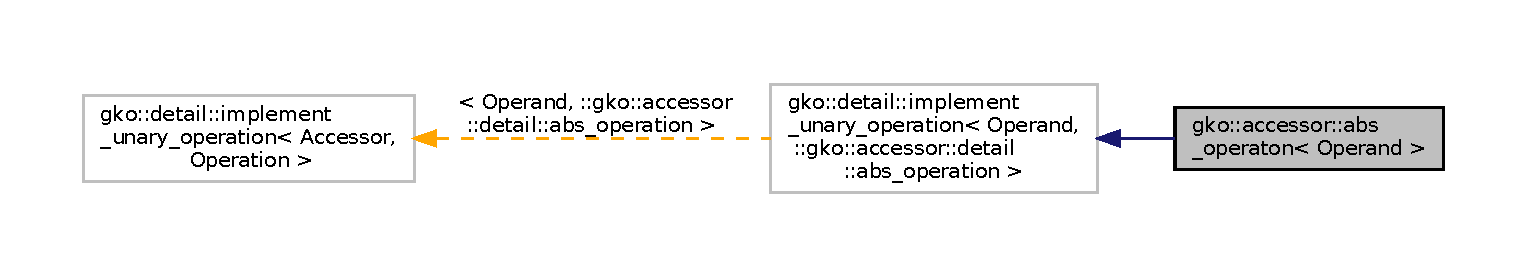
\includegraphics[width=350pt]{structgko_1_1accessor_1_1abs__operaton__coll__graph}
\end{center}
\end{figure}


The documentation for this struct was generated from the following file\+:\begin{DoxyCompactItemize}
\item 
ginkgo/core/base/range.\+hpp (357228f4e)\end{DoxyCompactItemize}

\hypertarget{classgko_1_1AbstractFactory}{}\section{gko\+:\+:Abstract\+Factory$<$ Abstract\+Product\+Type, Components\+Type $>$ Class Template Reference}
\label{classgko_1_1AbstractFactory}\index{gko\+::\+Abstract\+Factory$<$ Abstract\+Product\+Type, Components\+Type $>$@{gko\+::\+Abstract\+Factory$<$ Abstract\+Product\+Type, Components\+Type $>$}}


The \hyperlink{classgko_1_1AbstractFactory}{Abstract\+Factory} is a generic interface template that enables easy implementation of the abstract factory design pattern.  




{\ttfamily \#include $<$ginkgo/core/base/abstract\+\_\+factory.\+hpp$>$}



Collaboration diagram for gko\+:\+:Abstract\+Factory$<$ Abstract\+Product\+Type, Components\+Type $>$\+:
\nopagebreak
\begin{figure}[H]
\begin{center}
\leavevmode
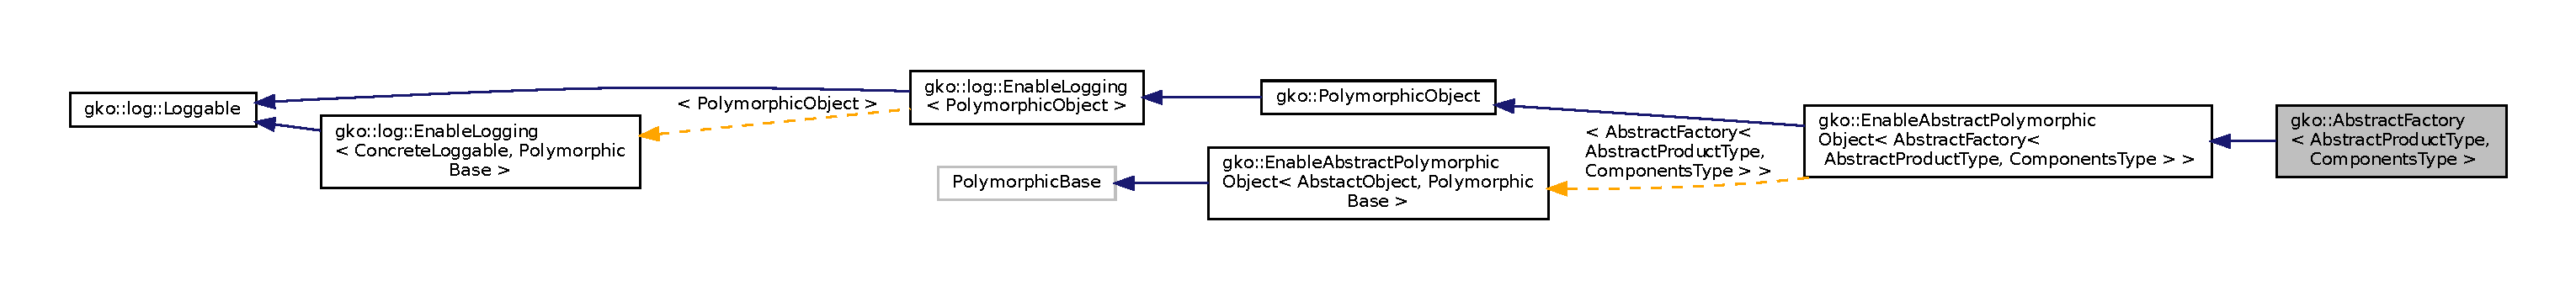
\includegraphics[width=350pt]{classgko_1_1AbstractFactory__coll__graph}
\end{center}
\end{figure}
\subsection*{Public Types}
\begin{DoxyCompactItemize}
\item 
\mbox{\Hypertarget{classgko_1_1AbstractFactory_afc8e23253c0fc2c81d6a74df19758454}\label{classgko_1_1AbstractFactory_afc8e23253c0fc2c81d6a74df19758454}} 
using {\bfseries abstract\+\_\+product\+\_\+type} = Abstract\+Product\+Type
\item 
\mbox{\Hypertarget{classgko_1_1AbstractFactory_aca858cfbda0fb1e8df67eca429971c61}\label{classgko_1_1AbstractFactory_aca858cfbda0fb1e8df67eca429971c61}} 
using {\bfseries components\+\_\+type} = Components\+Type
\end{DoxyCompactItemize}
\subsection*{Public Member Functions}
\begin{DoxyCompactItemize}
\item 
{\footnotesize template$<$typename... Args$>$ }\\std\+::unique\+\_\+ptr$<$ Abstract\+Product\+Type $>$ \hyperlink{classgko_1_1AbstractFactory_a159c45f1db78b6b928d69cb9adf5c9ee}{generate} (Args \&\&... args) const
\begin{DoxyCompactList}\small\item\em Creates a new product from the given components. \end{DoxyCompactList}\end{DoxyCompactItemize}


\subsection{Detailed Description}
\subsubsection*{template$<$typename Abstract\+Product\+Type, typename Components\+Type$>$\newline
class gko\+::\+Abstract\+Factory$<$ Abstract\+Product\+Type, Components\+Type $>$}

The \hyperlink{classgko_1_1AbstractFactory}{Abstract\+Factory} is a generic interface template that enables easy implementation of the abstract factory design pattern. 

The interface provides the \hyperlink{classgko_1_1AbstractFactory_a159c45f1db78b6b928d69cb9adf5c9ee}{Abstract\+Factory\+::generate()} method that can produce products of type {\ttfamily Abstract\+Product\+Type} using an object of {\ttfamily Components\+Type} (which can be constructed on the fly from parameters to its constructors). The \hyperlink{classgko_1_1AbstractFactory_a159c45f1db78b6b928d69cb9adf5c9ee}{generate()} method is not declared as virtual, as this allows subclasses to hide the method with a variant that preserves the compile-\/time type of the objects. Instead, implementers should override the generate\+\_\+impl() method, which is declared virtual.

Implementers of concrete factories should consider using the \hyperlink{classgko_1_1EnableDefaultFactory}{Enable\+Default\+Factory} mixin to obtain default implementations of utility methods of \hyperlink{classgko_1_1PolymorphicObject}{Polymorphic\+Object} and \hyperlink{classgko_1_1AbstractFactory}{Abstract\+Factory}.


\begin{DoxyTemplParams}{Template Parameters}
{\em Abstract\+Product\+Type} & the type of products the factory produces \\
\hline
{\em Components\+Type} & the type of components the factory needs to produce the product \\
\hline
\end{DoxyTemplParams}


\subsection{Member Function Documentation}
\mbox{\Hypertarget{classgko_1_1AbstractFactory_a159c45f1db78b6b928d69cb9adf5c9ee}\label{classgko_1_1AbstractFactory_a159c45f1db78b6b928d69cb9adf5c9ee}} 
\index{gko\+::\+Abstract\+Factory@{gko\+::\+Abstract\+Factory}!generate@{generate}}
\index{generate@{generate}!gko\+::\+Abstract\+Factory@{gko\+::\+Abstract\+Factory}}
\subsubsection{\texorpdfstring{generate()}{generate()}}
{\footnotesize\ttfamily template$<$typename Abstract\+Product\+Type, typename Components\+Type$>$ \\
template$<$typename... Args$>$ \\
std\+::unique\+\_\+ptr$<$Abstract\+Product\+Type$>$ \hyperlink{classgko_1_1AbstractFactory}{gko\+::\+Abstract\+Factory}$<$ Abstract\+Product\+Type, Components\+Type $>$\+::generate (\begin{DoxyParamCaption}\item[{Args \&\&...}]{args }\end{DoxyParamCaption}) const\hspace{0.3cm}{\ttfamily [inline]}}



Creates a new product from the given components. 

The method will create an Components\+Type object from the arguments of this method, and pass it to the generate\+\_\+impl() function which will create a new Abstract\+Product\+Type.


\begin{DoxyTemplParams}{Template Parameters}
{\em Args} & types of arguments passed to the constructor of Components\+Type\\
\hline
\end{DoxyTemplParams}

\begin{DoxyParams}{Parameters}
{\em args} & arguments passed to the constructor of Components\+Type\\
\hline
\end{DoxyParams}
\begin{DoxyReturn}{Returns}
an instance of Abstract\+Product\+Type 
\end{DoxyReturn}


The documentation for this class was generated from the following file\+:\begin{DoxyCompactItemize}
\item 
ginkgo/core/base/abstract\+\_\+factory.\+hpp (fd80b3c2)\end{DoxyCompactItemize}

\hypertarget{structgko_1_1accessor_1_1add}{}\section{gko\+:\+:accessor\+:\+:add$<$ Kind, First\+Operand, Second\+Operand $>$ Struct Template Reference}
\label{structgko_1_1accessor_1_1add}\index{gko\+::accessor\+::add$<$ Kind, First\+Operand, Second\+Operand $>$@{gko\+::accessor\+::add$<$ Kind, First\+Operand, Second\+Operand $>$}}


Collaboration diagram for gko\+:\+:accessor\+:\+:add$<$ Kind, First\+Operand, Second\+Operand $>$\+:
\nopagebreak
\begin{figure}[H]
\begin{center}
\leavevmode
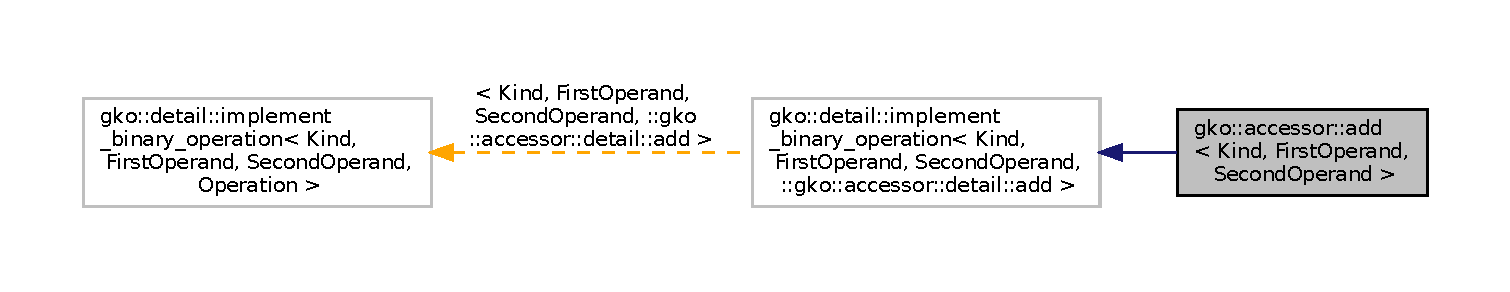
\includegraphics[width=350pt]{structgko_1_1accessor_1_1add__coll__graph}
\end{center}
\end{figure}


The documentation for this struct was generated from the following file\+:\begin{DoxyCompactItemize}
\item 
ginkgo/core/base/range.\+hpp (c71510aa)\end{DoxyCompactItemize}

\hypertarget{classgko_1_1AllocationError}{}\section{gko\+:\+:Allocation\+Error Class Reference}
\label{classgko_1_1AllocationError}\index{gko\+::\+Allocation\+Error@{gko\+::\+Allocation\+Error}}


\hyperlink{classgko_1_1AllocationError}{Allocation\+Error} is thrown if a memory allocation fails.  




{\ttfamily \#include $<$ginkgo/core/base/exception.\+hpp$>$}



Collaboration diagram for gko\+:\+:Allocation\+Error\+:
\nopagebreak
\begin{figure}[H]
\begin{center}
\leavevmode
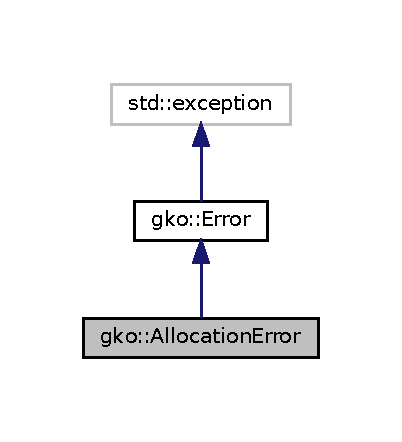
\includegraphics[width=193pt]{classgko_1_1AllocationError__coll__graph}
\end{center}
\end{figure}
\subsection*{Public Member Functions}
\begin{DoxyCompactItemize}
\item 
\hyperlink{classgko_1_1AllocationError_ab06f1e22cd0cd39acab7cd5e96f2f9ca}{Allocation\+Error} (const std\+::string \&file, int line, const std\+::string \&device, \hyperlink{namespacegko_a6e5c95df0ae4e47aab2f604a22d98ee7}{size\+\_\+type} bytes)
\begin{DoxyCompactList}\small\item\em Initializes an allocation error. \end{DoxyCompactList}\end{DoxyCompactItemize}


\subsection{Detailed Description}
\hyperlink{classgko_1_1AllocationError}{Allocation\+Error} is thrown if a memory allocation fails. 

\subsection{Constructor \& Destructor Documentation}
\mbox{\Hypertarget{classgko_1_1AllocationError_ab06f1e22cd0cd39acab7cd5e96f2f9ca}\label{classgko_1_1AllocationError_ab06f1e22cd0cd39acab7cd5e96f2f9ca}} 
\index{gko\+::\+Allocation\+Error@{gko\+::\+Allocation\+Error}!Allocation\+Error@{Allocation\+Error}}
\index{Allocation\+Error@{Allocation\+Error}!gko\+::\+Allocation\+Error@{gko\+::\+Allocation\+Error}}
\subsubsection{\texorpdfstring{Allocation\+Error()}{AllocationError()}}
{\footnotesize\ttfamily gko\+::\+Allocation\+Error\+::\+Allocation\+Error (\begin{DoxyParamCaption}\item[{const std\+::string \&}]{file,  }\item[{int}]{line,  }\item[{const std\+::string \&}]{device,  }\item[{\hyperlink{namespacegko_a6e5c95df0ae4e47aab2f604a22d98ee7}{size\+\_\+type}}]{bytes }\end{DoxyParamCaption})}



Initializes an allocation error. 


\begin{DoxyParams}{Parameters}
{\em file} & The name of the offending source file \\
\hline
{\em line} & The source code line number where the error occurred \\
\hline
{\em device} & The device on which the error occurred \\
\hline
{\em bytes} & The size of the memory block whose allocation failed. \\
\hline
\end{DoxyParams}


The documentation for this class was generated from the following file\+:\begin{DoxyCompactItemize}
\item 
ginkgo/core/base/exception.\+hpp (99beb325)\end{DoxyCompactItemize}

\hypertarget{classgko_1_1Array}{}\doxysection{gko\+::Array$<$ Value\+Type $>$ Class Template Reference}
\label{classgko_1_1Array}\index{gko::Array$<$ ValueType $>$@{gko::Array$<$ ValueType $>$}}


An \mbox{\hyperlink{classgko_1_1Array}{Array}} is a container which encapsulates fixed-\/sized arrays, stored on the \mbox{\hyperlink{classgko_1_1Executor}{Executor}} tied to the \mbox{\hyperlink{classgko_1_1Array}{Array}}.  




{\ttfamily \#include $<$ginkgo/core/base/array.\+hpp$>$}

\doxysubsection*{Public Types}
\begin{DoxyCompactItemize}
\item 
\mbox{\Hypertarget{classgko_1_1Array_ad40c95e429262175cae51bcabd291a5b}\label{classgko_1_1Array_ad40c95e429262175cae51bcabd291a5b}} 
using \mbox{\hyperlink{classgko_1_1Array_ad40c95e429262175cae51bcabd291a5b}{value\+\_\+type}} = Value\+Type
\begin{DoxyCompactList}\small\item\em The type of elements stored in the array. \end{DoxyCompactList}\item 
\mbox{\Hypertarget{classgko_1_1Array_a39498b9cc303f4fa5685b2f98bb8ff4e}\label{classgko_1_1Array_a39498b9cc303f4fa5685b2f98bb8ff4e}} 
using \mbox{\hyperlink{classgko_1_1Array_a39498b9cc303f4fa5685b2f98bb8ff4e}{default\+\_\+deleter}} = \mbox{\hyperlink{classgko_1_1executor__deleter}{executor\+\_\+deleter}}$<$ \mbox{\hyperlink{classgko_1_1Array_ad40c95e429262175cae51bcabd291a5b}{value\+\_\+type}}\mbox{[}$\,$\mbox{]}$>$
\begin{DoxyCompactList}\small\item\em The default deleter type used by \mbox{\hyperlink{classgko_1_1Array}{Array}}. \end{DoxyCompactList}\item 
\mbox{\Hypertarget{classgko_1_1Array_af870dd6ab4ad4f7e0e20471cb17f4ad1}\label{classgko_1_1Array_af870dd6ab4ad4f7e0e20471cb17f4ad1}} 
using \mbox{\hyperlink{classgko_1_1Array_af870dd6ab4ad4f7e0e20471cb17f4ad1}{view\+\_\+deleter}} = \mbox{\hyperlink{classgko_1_1null__deleter}{null\+\_\+deleter}}$<$ \mbox{\hyperlink{classgko_1_1Array_ad40c95e429262175cae51bcabd291a5b}{value\+\_\+type}}\mbox{[}$\,$\mbox{]}$>$
\begin{DoxyCompactList}\small\item\em The deleter type used for views. \end{DoxyCompactList}\end{DoxyCompactItemize}
\doxysubsection*{Public Member Functions}
\begin{DoxyCompactItemize}
\item 
\mbox{\hyperlink{classgko_1_1Array_a6048d48c206e8dcae55e776b7adba06a}{Array}} () noexcept
\begin{DoxyCompactList}\small\item\em Creates an empty \mbox{\hyperlink{classgko_1_1Array}{Array}} not tied to any executor. \end{DoxyCompactList}\item 
\mbox{\hyperlink{classgko_1_1Array_ae64e4c698ecef2cfbe3ceb3dfd07dbaf}{Array}} (std\+::shared\+\_\+ptr$<$ const \mbox{\hyperlink{classgko_1_1Executor}{Executor}} $>$ exec) noexcept
\begin{DoxyCompactList}\small\item\em Creates an empty \mbox{\hyperlink{classgko_1_1Array}{Array}} tied to the specified \mbox{\hyperlink{classgko_1_1Executor}{Executor}}. \end{DoxyCompactList}\item 
\mbox{\hyperlink{classgko_1_1Array_a2cf49c2f39cbad160982d731fcf74031}{Array}} (std\+::shared\+\_\+ptr$<$ const \mbox{\hyperlink{classgko_1_1Executor}{Executor}} $>$ exec, \mbox{\hyperlink{namespacegko_a6e5c95df0ae4e47aab2f604a22d98ee7}{size\+\_\+type}} num\+\_\+elems)
\begin{DoxyCompactList}\small\item\em Creates an \mbox{\hyperlink{classgko_1_1Array}{Array}} on the specified \mbox{\hyperlink{classgko_1_1Executor}{Executor}}. \end{DoxyCompactList}\item 
{\footnotesize template$<$typename Deleter\+Type $>$ }\\\mbox{\hyperlink{classgko_1_1Array_a4aa436a039fe6a6391b810a44d0ca9c7}{Array}} (std\+::shared\+\_\+ptr$<$ const \mbox{\hyperlink{classgko_1_1Executor}{Executor}} $>$ exec, \mbox{\hyperlink{namespacegko_a6e5c95df0ae4e47aab2f604a22d98ee7}{size\+\_\+type}} num\+\_\+elems, \mbox{\hyperlink{classgko_1_1Array_ad40c95e429262175cae51bcabd291a5b}{value\+\_\+type}} $\ast$data, Deleter\+Type deleter)
\begin{DoxyCompactList}\small\item\em Creates an \mbox{\hyperlink{classgko_1_1Array}{Array}} from existing memory. \end{DoxyCompactList}\item 
\mbox{\hyperlink{classgko_1_1Array_afdf9ea91228cf272e3b5f18cc5dff2a8}{Array}} (std\+::shared\+\_\+ptr$<$ const \mbox{\hyperlink{classgko_1_1Executor}{Executor}} $>$ exec, \mbox{\hyperlink{namespacegko_a6e5c95df0ae4e47aab2f604a22d98ee7}{size\+\_\+type}} num\+\_\+elems, \mbox{\hyperlink{classgko_1_1Array_ad40c95e429262175cae51bcabd291a5b}{value\+\_\+type}} $\ast$data)
\begin{DoxyCompactList}\small\item\em Creates an \mbox{\hyperlink{classgko_1_1Array}{Array}} from existing memory. \end{DoxyCompactList}\item 
{\footnotesize template$<$typename Random\+Access\+Iterator $>$ }\\\mbox{\hyperlink{classgko_1_1Array_a473ac8d0d3fa05918064cb5f26c3a540}{Array}} (std\+::shared\+\_\+ptr$<$ const \mbox{\hyperlink{classgko_1_1Executor}{Executor}} $>$ exec, Random\+Access\+Iterator begin, Random\+Access\+Iterator end)
\begin{DoxyCompactList}\small\item\em Creates an array on the specified \mbox{\hyperlink{classgko_1_1Executor}{Executor}} and initializes it with values. \end{DoxyCompactList}\item 
{\footnotesize template$<$typename T $>$ }\\\mbox{\hyperlink{classgko_1_1Array_aa0aa5ae24d1006778bba7ef7419439b2}{Array}} (std\+::shared\+\_\+ptr$<$ const \mbox{\hyperlink{classgko_1_1Executor}{Executor}} $>$ exec, std\+::initializer\+\_\+list$<$ T $>$ init\+\_\+list)
\begin{DoxyCompactList}\small\item\em Creates an array on the specified \mbox{\hyperlink{classgko_1_1Executor}{Executor}} and initializes it with values. \end{DoxyCompactList}\item 
\mbox{\hyperlink{classgko_1_1Array_ad03ebd9c7e7d63fc3b8b7a0a9ba8d16b}{Array}} (std\+::shared\+\_\+ptr$<$ const \mbox{\hyperlink{classgko_1_1Executor}{Executor}} $>$ exec, const \mbox{\hyperlink{classgko_1_1Array}{Array}} \&other)
\begin{DoxyCompactList}\small\item\em Creates a copy of another array on a different executor. \end{DoxyCompactList}\item 
\mbox{\hyperlink{classgko_1_1Array_ab5c0cdf59d9920d0f72f4018a5e4a8ab}{Array}} (const \mbox{\hyperlink{classgko_1_1Array}{Array}} \&other)
\begin{DoxyCompactList}\small\item\em Creates a copy of another array. \end{DoxyCompactList}\item 
\mbox{\hyperlink{classgko_1_1Array_a7e5b32002ac86e0534b91a4808212e28}{Array}} (std\+::shared\+\_\+ptr$<$ const \mbox{\hyperlink{classgko_1_1Executor}{Executor}} $>$ exec, \mbox{\hyperlink{classgko_1_1Array}{Array}} \&\&other)
\begin{DoxyCompactList}\small\item\em Moves another array to a different executor. \end{DoxyCompactList}\item 
\mbox{\hyperlink{classgko_1_1Array_a29da5ccbf776b7c85dbda0e8b4f20647}{Array}} (\mbox{\hyperlink{classgko_1_1Array}{Array}} \&\&other)
\begin{DoxyCompactList}\small\item\em Moves another array. \end{DoxyCompactList}\item 
\mbox{\hyperlink{classgko_1_1Array}{Array}} \& \mbox{\hyperlink{classgko_1_1Array_a841412d7a03b8210ba39e77b3bd05ce3}{operator=}} (const \mbox{\hyperlink{classgko_1_1Array}{Array}} \&other)
\begin{DoxyCompactList}\small\item\em Copies data from another array or view. \end{DoxyCompactList}\item 
\mbox{\hyperlink{classgko_1_1Array}{Array}} \& \mbox{\hyperlink{classgko_1_1Array_a62d5346849e3943a5fcac962e344ab58}{operator=}} (\mbox{\hyperlink{classgko_1_1Array}{Array}} \&\&other)
\begin{DoxyCompactList}\small\item\em Moves data from another array or view. \end{DoxyCompactList}\item 
{\footnotesize template$<$typename Other\+Value\+Type $>$ }\\xstd\+::enable\+\_\+if\+\_\+t$<$!std\+::is\+\_\+same$<$ Value\+Type, Other\+Value\+Type $>$\+::value, \mbox{\hyperlink{classgko_1_1Array}{Array}} $>$ \& \mbox{\hyperlink{classgko_1_1Array_ad27c8f6831d9a360d8f11b25ce274acc}{operator=}} (const \mbox{\hyperlink{classgko_1_1Array}{Array}}$<$ Other\+Value\+Type $>$ \&other)
\begin{DoxyCompactList}\small\item\em Copies and converts data from another array with another data type. \end{DoxyCompactList}\item 
void \mbox{\hyperlink{classgko_1_1Array_a64f7e9f19c4e8cff8adb402da70476c3}{clear}} () noexcept
\begin{DoxyCompactList}\small\item\em Deallocates all data used by the \mbox{\hyperlink{classgko_1_1Array}{Array}}. \end{DoxyCompactList}\item 
void \mbox{\hyperlink{classgko_1_1Array_ab42114c635a05ecff66e1ab5e5074d14}{resize\+\_\+and\+\_\+reset}} (\mbox{\hyperlink{namespacegko_a6e5c95df0ae4e47aab2f604a22d98ee7}{size\+\_\+type}} num\+\_\+elems)
\begin{DoxyCompactList}\small\item\em Resizes the array so it is able to hold the specified number of elements. \end{DoxyCompactList}\item 
\mbox{\hyperlink{namespacegko_a6e5c95df0ae4e47aab2f604a22d98ee7}{size\+\_\+type}} \mbox{\hyperlink{classgko_1_1Array_ad4a2aa179d350634e6579f144b6b2cf0}{get\+\_\+num\+\_\+elems}} () const noexcept
\begin{DoxyCompactList}\small\item\em Returns the number of elements in the \mbox{\hyperlink{classgko_1_1Array}{Array}}. \end{DoxyCompactList}\item 
\mbox{\hyperlink{classgko_1_1Array_ad40c95e429262175cae51bcabd291a5b}{value\+\_\+type}} $\ast$ \mbox{\hyperlink{classgko_1_1Array_a9acf29878703bb8767e3cea2ba499dae}{get\+\_\+data}} () noexcept
\begin{DoxyCompactList}\small\item\em Returns a pointer to the block of memory used to store the elements of the \mbox{\hyperlink{classgko_1_1Array}{Array}}. \end{DoxyCompactList}\item 
const \mbox{\hyperlink{classgko_1_1Array_ad40c95e429262175cae51bcabd291a5b}{value\+\_\+type}} $\ast$ \mbox{\hyperlink{classgko_1_1Array_a5a46e0920b649cdb062f5e415922d1aa}{get\+\_\+const\+\_\+data}} () const noexcept
\begin{DoxyCompactList}\small\item\em Returns a constant pointer to the block of memory used to store the elements of the \mbox{\hyperlink{classgko_1_1Array}{Array}}. \end{DoxyCompactList}\item 
std\+::shared\+\_\+ptr$<$ const \mbox{\hyperlink{classgko_1_1Executor}{Executor}} $>$ \mbox{\hyperlink{classgko_1_1Array_a820e5930cb5072acc7673fdb2d11efcd}{get\+\_\+executor}} () const noexcept
\begin{DoxyCompactList}\small\item\em Returns the \mbox{\hyperlink{classgko_1_1Executor}{Executor}} associated with the array. \end{DoxyCompactList}\item 
void \mbox{\hyperlink{classgko_1_1Array_a44dd24e909f518f08320c3065e087d85}{set\+\_\+executor}} (std\+::shared\+\_\+ptr$<$ const \mbox{\hyperlink{classgko_1_1Executor}{Executor}} $>$ exec)
\begin{DoxyCompactList}\small\item\em Changes the \mbox{\hyperlink{classgko_1_1Executor}{Executor}} of the \mbox{\hyperlink{classgko_1_1Array}{Array}}, moving the allocated data to the new \mbox{\hyperlink{classgko_1_1Executor}{Executor}}. \end{DoxyCompactList}\item 
bool \mbox{\hyperlink{classgko_1_1Array_a18164d25e9e87bdc6b8af7ce9956199a}{is\+\_\+owning}} ()
\begin{DoxyCompactList}\small\item\em Tells whether this \mbox{\hyperlink{classgko_1_1Array}{Array}} owns its data or not. \end{DoxyCompactList}\end{DoxyCompactItemize}
\doxysubsection*{Static Public Member Functions}
\begin{DoxyCompactItemize}
\item 
static \mbox{\hyperlink{classgko_1_1Array}{Array}} \mbox{\hyperlink{classgko_1_1Array_ae8e2b4841e60741227daf3367de6ecde}{view}} (std\+::shared\+\_\+ptr$<$ const \mbox{\hyperlink{classgko_1_1Executor}{Executor}} $>$ exec, \mbox{\hyperlink{namespacegko_a6e5c95df0ae4e47aab2f604a22d98ee7}{size\+\_\+type}} num\+\_\+elems, \mbox{\hyperlink{classgko_1_1Array_ad40c95e429262175cae51bcabd291a5b}{value\+\_\+type}} $\ast$data)
\begin{DoxyCompactList}\small\item\em Creates an \mbox{\hyperlink{classgko_1_1Array}{Array}} from existing memory. \end{DoxyCompactList}\end{DoxyCompactItemize}
\doxysubsection*{Friends}
\begin{DoxyCompactItemize}
\item 
\mbox{\Hypertarget{classgko_1_1Array_ab1a595168ea1870ce436dfd2d8e69b6d}\label{classgko_1_1Array_ab1a595168ea1870ce436dfd2d8e69b6d}} 
{\footnotesize template$<$typename Other\+Value\+Type $>$ }\\class {\bfseries Array}
\end{DoxyCompactItemize}


\doxysubsection{Detailed Description}
\subsubsection*{template$<$typename Value\+Type$>$\newline
class gko\+::\+Array$<$ Value\+Type $>$}

An \mbox{\hyperlink{classgko_1_1Array}{Array}} is a container which encapsulates fixed-\/sized arrays, stored on the \mbox{\hyperlink{classgko_1_1Executor}{Executor}} tied to the \mbox{\hyperlink{classgko_1_1Array}{Array}}. 

The array stores and transfers its data as {\bfseries{raw}} memory, which means that the constructors of its elements are not called when constructing, copying or moving the \mbox{\hyperlink{classgko_1_1Array}{Array}}. Thus, the \mbox{\hyperlink{classgko_1_1Array}{Array}} class is most suitable for storing P\+OD types.


\begin{DoxyTemplParams}{Template Parameters}
{\em Value\+Type} & the type of elements stored in the array \\
\hline
\end{DoxyTemplParams}


\doxysubsection{Constructor \& Destructor Documentation}
\mbox{\Hypertarget{classgko_1_1Array_a6048d48c206e8dcae55e776b7adba06a}\label{classgko_1_1Array_a6048d48c206e8dcae55e776b7adba06a}} 
\index{gko::Array$<$ ValueType $>$@{gko::Array$<$ ValueType $>$}!Array@{Array}}
\index{Array@{Array}!gko::Array$<$ ValueType $>$@{gko::Array$<$ ValueType $>$}}
\doxysubsubsection{\texorpdfstring{Array()}{Array()}\hspace{0.1cm}{\footnotesize\ttfamily [1/11]}}
{\footnotesize\ttfamily template$<$typename Value\+Type$>$ \\
\mbox{\hyperlink{classgko_1_1Array}{gko\+::\+Array}}$<$ Value\+Type $>$\+::\mbox{\hyperlink{classgko_1_1Array}{Array}} (\begin{DoxyParamCaption}{ }\end{DoxyParamCaption})\hspace{0.3cm}{\ttfamily [inline]}, {\ttfamily [noexcept]}}



Creates an empty \mbox{\hyperlink{classgko_1_1Array}{Array}} not tied to any executor. 

An array without an assigned executor can only be empty. Attempts to change its size (e.\+g. via the resize\+\_\+and\+\_\+reset method) will result in an exception. If such an array is used as the right hand side of an assignment or move assignment expression, the data of the target array will be cleared, but its executor will not be modified.

The executor can later be set by using the set\+\_\+executor method. If an \mbox{\hyperlink{classgko_1_1Array}{Array}} with no assigned executor is assigned or moved to, it will inherit the executor of the source \mbox{\hyperlink{classgko_1_1Array}{Array}}. \mbox{\Hypertarget{classgko_1_1Array_ae64e4c698ecef2cfbe3ceb3dfd07dbaf}\label{classgko_1_1Array_ae64e4c698ecef2cfbe3ceb3dfd07dbaf}} 
\index{gko::Array$<$ ValueType $>$@{gko::Array$<$ ValueType $>$}!Array@{Array}}
\index{Array@{Array}!gko::Array$<$ ValueType $>$@{gko::Array$<$ ValueType $>$}}
\doxysubsubsection{\texorpdfstring{Array()}{Array()}\hspace{0.1cm}{\footnotesize\ttfamily [2/11]}}
{\footnotesize\ttfamily template$<$typename Value\+Type$>$ \\
\mbox{\hyperlink{classgko_1_1Array}{gko\+::\+Array}}$<$ Value\+Type $>$\+::\mbox{\hyperlink{classgko_1_1Array}{Array}} (\begin{DoxyParamCaption}\item[{std\+::shared\+\_\+ptr$<$ const \mbox{\hyperlink{classgko_1_1Executor}{Executor}} $>$}]{exec }\end{DoxyParamCaption})\hspace{0.3cm}{\ttfamily [inline]}, {\ttfamily [noexcept]}}



Creates an empty \mbox{\hyperlink{classgko_1_1Array}{Array}} tied to the specified \mbox{\hyperlink{classgko_1_1Executor}{Executor}}. 


\begin{DoxyParams}{Parameters}
{\em exec} & the \mbox{\hyperlink{classgko_1_1Executor}{Executor}} where the array data is allocated \\
\hline
\end{DoxyParams}
\mbox{\Hypertarget{classgko_1_1Array_a2cf49c2f39cbad160982d731fcf74031}\label{classgko_1_1Array_a2cf49c2f39cbad160982d731fcf74031}} 
\index{gko::Array$<$ ValueType $>$@{gko::Array$<$ ValueType $>$}!Array@{Array}}
\index{Array@{Array}!gko::Array$<$ ValueType $>$@{gko::Array$<$ ValueType $>$}}
\doxysubsubsection{\texorpdfstring{Array()}{Array()}\hspace{0.1cm}{\footnotesize\ttfamily [3/11]}}
{\footnotesize\ttfamily template$<$typename Value\+Type$>$ \\
\mbox{\hyperlink{classgko_1_1Array}{gko\+::\+Array}}$<$ Value\+Type $>$\+::\mbox{\hyperlink{classgko_1_1Array}{Array}} (\begin{DoxyParamCaption}\item[{std\+::shared\+\_\+ptr$<$ const \mbox{\hyperlink{classgko_1_1Executor}{Executor}} $>$}]{exec,  }\item[{\mbox{\hyperlink{namespacegko_a6e5c95df0ae4e47aab2f604a22d98ee7}{size\+\_\+type}}}]{num\+\_\+elems }\end{DoxyParamCaption})\hspace{0.3cm}{\ttfamily [inline]}}



Creates an \mbox{\hyperlink{classgko_1_1Array}{Array}} on the specified \mbox{\hyperlink{classgko_1_1Executor}{Executor}}. 


\begin{DoxyParams}{Parameters}
{\em exec} & the \mbox{\hyperlink{classgko_1_1Executor}{Executor}} where the array data will be allocated \\
\hline
{\em num\+\_\+elems} & the amount of memory (expressed as the number of {\ttfamily value\+\_\+type} elements) allocated on the \mbox{\hyperlink{classgko_1_1Executor}{Executor}} \\
\hline
\end{DoxyParams}
\mbox{\Hypertarget{classgko_1_1Array_a4aa436a039fe6a6391b810a44d0ca9c7}\label{classgko_1_1Array_a4aa436a039fe6a6391b810a44d0ca9c7}} 
\index{gko::Array$<$ ValueType $>$@{gko::Array$<$ ValueType $>$}!Array@{Array}}
\index{Array@{Array}!gko::Array$<$ ValueType $>$@{gko::Array$<$ ValueType $>$}}
\doxysubsubsection{\texorpdfstring{Array()}{Array()}\hspace{0.1cm}{\footnotesize\ttfamily [4/11]}}
{\footnotesize\ttfamily template$<$typename Value\+Type$>$ \\
template$<$typename Deleter\+Type $>$ \\
\mbox{\hyperlink{classgko_1_1Array}{gko\+::\+Array}}$<$ Value\+Type $>$\+::\mbox{\hyperlink{classgko_1_1Array}{Array}} (\begin{DoxyParamCaption}\item[{std\+::shared\+\_\+ptr$<$ const \mbox{\hyperlink{classgko_1_1Executor}{Executor}} $>$}]{exec,  }\item[{\mbox{\hyperlink{namespacegko_a6e5c95df0ae4e47aab2f604a22d98ee7}{size\+\_\+type}}}]{num\+\_\+elems,  }\item[{\mbox{\hyperlink{classgko_1_1Array_ad40c95e429262175cae51bcabd291a5b}{value\+\_\+type}} $\ast$}]{data,  }\item[{Deleter\+Type}]{deleter }\end{DoxyParamCaption})\hspace{0.3cm}{\ttfamily [inline]}}



Creates an \mbox{\hyperlink{classgko_1_1Array}{Array}} from existing memory. 

The memory will be managed by the array, and deallocated using the specified deleter (e.\+g. use std\+::default\+\_\+delete for data allocated with new).


\begin{DoxyTemplParams}{Template Parameters}
{\em Deleter\+Type} & type of the deleter\\
\hline
\end{DoxyTemplParams}

\begin{DoxyParams}{Parameters}
{\em exec} & executor where {\ttfamily data} is located \\
\hline
{\em num\+\_\+elems} & number of elements in {\ttfamily data} \\
\hline
{\em data} & chunk of memory used to create the array \\
\hline
{\em deleter} & the deleter used to free the memory\\
\hline
\end{DoxyParams}
\begin{DoxySeeAlso}{See also}
\mbox{\hyperlink{classgko_1_1Array_ae8e2b4841e60741227daf3367de6ecde}{Array\+::view()}} to create an \mbox{\hyperlink{namespacegko_ae749a5ea11a93c1bcc9158d9a6e9fb68af1f713c9e000f5d3f280adbd124df4f5}{array}} that does not deallocate memory 

Array(std\+::shared\+\_\+ptr$<$cont Executor$>$, size\+\_\+type, value\+\_\+type$\ast$) to deallocate the memory using \mbox{\hyperlink{classgko_1_1Executor_a0befe43d21c93e199d1620eaae4ccc0c}{Executor\+::free()}} method 
\end{DoxySeeAlso}
\mbox{\Hypertarget{classgko_1_1Array_afdf9ea91228cf272e3b5f18cc5dff2a8}\label{classgko_1_1Array_afdf9ea91228cf272e3b5f18cc5dff2a8}} 
\index{gko::Array$<$ ValueType $>$@{gko::Array$<$ ValueType $>$}!Array@{Array}}
\index{Array@{Array}!gko::Array$<$ ValueType $>$@{gko::Array$<$ ValueType $>$}}
\doxysubsubsection{\texorpdfstring{Array()}{Array()}\hspace{0.1cm}{\footnotesize\ttfamily [5/11]}}
{\footnotesize\ttfamily template$<$typename Value\+Type$>$ \\
\mbox{\hyperlink{classgko_1_1Array}{gko\+::\+Array}}$<$ Value\+Type $>$\+::\mbox{\hyperlink{classgko_1_1Array}{Array}} (\begin{DoxyParamCaption}\item[{std\+::shared\+\_\+ptr$<$ const \mbox{\hyperlink{classgko_1_1Executor}{Executor}} $>$}]{exec,  }\item[{\mbox{\hyperlink{namespacegko_a6e5c95df0ae4e47aab2f604a22d98ee7}{size\+\_\+type}}}]{num\+\_\+elems,  }\item[{\mbox{\hyperlink{classgko_1_1Array_ad40c95e429262175cae51bcabd291a5b}{value\+\_\+type}} $\ast$}]{data }\end{DoxyParamCaption})\hspace{0.3cm}{\ttfamily [inline]}}



Creates an \mbox{\hyperlink{classgko_1_1Array}{Array}} from existing memory. 

The memory will be managed by the array, and deallocated using the \mbox{\hyperlink{classgko_1_1Executor_a0befe43d21c93e199d1620eaae4ccc0c}{Executor\+::free}} method.


\begin{DoxyParams}{Parameters}
{\em exec} & executor where {\ttfamily data} is located \\
\hline
{\em num\+\_\+elems} & number of elements in {\ttfamily data} \\
\hline
{\em data} & chunk of memory used to create the array \\
\hline
\end{DoxyParams}
\mbox{\Hypertarget{classgko_1_1Array_a473ac8d0d3fa05918064cb5f26c3a540}\label{classgko_1_1Array_a473ac8d0d3fa05918064cb5f26c3a540}} 
\index{gko::Array$<$ ValueType $>$@{gko::Array$<$ ValueType $>$}!Array@{Array}}
\index{Array@{Array}!gko::Array$<$ ValueType $>$@{gko::Array$<$ ValueType $>$}}
\doxysubsubsection{\texorpdfstring{Array()}{Array()}\hspace{0.1cm}{\footnotesize\ttfamily [6/11]}}
{\footnotesize\ttfamily template$<$typename Value\+Type$>$ \\
template$<$typename Random\+Access\+Iterator $>$ \\
\mbox{\hyperlink{classgko_1_1Array}{gko\+::\+Array}}$<$ Value\+Type $>$\+::\mbox{\hyperlink{classgko_1_1Array}{Array}} (\begin{DoxyParamCaption}\item[{std\+::shared\+\_\+ptr$<$ const \mbox{\hyperlink{classgko_1_1Executor}{Executor}} $>$}]{exec,  }\item[{Random\+Access\+Iterator}]{begin,  }\item[{Random\+Access\+Iterator}]{end }\end{DoxyParamCaption})\hspace{0.3cm}{\ttfamily [inline]}}



Creates an array on the specified \mbox{\hyperlink{classgko_1_1Executor}{Executor}} and initializes it with values. 


\begin{DoxyTemplParams}{Template Parameters}
{\em Random\+Access\+Iterator} & type of the iterators\\
\hline
\end{DoxyTemplParams}

\begin{DoxyParams}{Parameters}
{\em exec} & the \mbox{\hyperlink{classgko_1_1Executor}{Executor}} where the array data will be allocated \\
\hline
{\em begin} & start of range of values \\
\hline
{\em end} & end of range of values \\
\hline
\end{DoxyParams}
\mbox{\Hypertarget{classgko_1_1Array_aa0aa5ae24d1006778bba7ef7419439b2}\label{classgko_1_1Array_aa0aa5ae24d1006778bba7ef7419439b2}} 
\index{gko::Array$<$ ValueType $>$@{gko::Array$<$ ValueType $>$}!Array@{Array}}
\index{Array@{Array}!gko::Array$<$ ValueType $>$@{gko::Array$<$ ValueType $>$}}
\doxysubsubsection{\texorpdfstring{Array()}{Array()}\hspace{0.1cm}{\footnotesize\ttfamily [7/11]}}
{\footnotesize\ttfamily template$<$typename Value\+Type$>$ \\
template$<$typename T $>$ \\
\mbox{\hyperlink{classgko_1_1Array}{gko\+::\+Array}}$<$ Value\+Type $>$\+::\mbox{\hyperlink{classgko_1_1Array}{Array}} (\begin{DoxyParamCaption}\item[{std\+::shared\+\_\+ptr$<$ const \mbox{\hyperlink{classgko_1_1Executor}{Executor}} $>$}]{exec,  }\item[{std\+::initializer\+\_\+list$<$ T $>$}]{init\+\_\+list }\end{DoxyParamCaption})\hspace{0.3cm}{\ttfamily [inline]}}



Creates an array on the specified \mbox{\hyperlink{classgko_1_1Executor}{Executor}} and initializes it with values. 


\begin{DoxyTemplParams}{Template Parameters}
{\em T} & type of values used to initialize the array (T has to be implicitly convertible to value\+\_\+type)\\
\hline
\end{DoxyTemplParams}

\begin{DoxyParams}{Parameters}
{\em exec} & the \mbox{\hyperlink{classgko_1_1Executor}{Executor}} where the array data will be allocated \\
\hline
{\em init\+\_\+list} & list of values used to initialize the \mbox{\hyperlink{classgko_1_1Array}{Array}} \\
\hline
\end{DoxyParams}
\mbox{\Hypertarget{classgko_1_1Array_ad03ebd9c7e7d63fc3b8b7a0a9ba8d16b}\label{classgko_1_1Array_ad03ebd9c7e7d63fc3b8b7a0a9ba8d16b}} 
\index{gko::Array$<$ ValueType $>$@{gko::Array$<$ ValueType $>$}!Array@{Array}}
\index{Array@{Array}!gko::Array$<$ ValueType $>$@{gko::Array$<$ ValueType $>$}}
\doxysubsubsection{\texorpdfstring{Array()}{Array()}\hspace{0.1cm}{\footnotesize\ttfamily [8/11]}}
{\footnotesize\ttfamily template$<$typename Value\+Type$>$ \\
\mbox{\hyperlink{classgko_1_1Array}{gko\+::\+Array}}$<$ Value\+Type $>$\+::\mbox{\hyperlink{classgko_1_1Array}{Array}} (\begin{DoxyParamCaption}\item[{std\+::shared\+\_\+ptr$<$ const \mbox{\hyperlink{classgko_1_1Executor}{Executor}} $>$}]{exec,  }\item[{const \mbox{\hyperlink{classgko_1_1Array}{Array}}$<$ Value\+Type $>$ \&}]{other }\end{DoxyParamCaption})\hspace{0.3cm}{\ttfamily [inline]}}



Creates a copy of another array on a different executor. 

This does not invoke the constructors of the elements, instead they are copied as P\+OD types.


\begin{DoxyParams}{Parameters}
{\em exec} & the executor where the new array will be created \\
\hline
{\em other} & the \mbox{\hyperlink{classgko_1_1Array}{Array}} to copy from \\
\hline
\end{DoxyParams}
\mbox{\Hypertarget{classgko_1_1Array_ab5c0cdf59d9920d0f72f4018a5e4a8ab}\label{classgko_1_1Array_ab5c0cdf59d9920d0f72f4018a5e4a8ab}} 
\index{gko::Array$<$ ValueType $>$@{gko::Array$<$ ValueType $>$}!Array@{Array}}
\index{Array@{Array}!gko::Array$<$ ValueType $>$@{gko::Array$<$ ValueType $>$}}
\doxysubsubsection{\texorpdfstring{Array()}{Array()}\hspace{0.1cm}{\footnotesize\ttfamily [9/11]}}
{\footnotesize\ttfamily template$<$typename Value\+Type$>$ \\
\mbox{\hyperlink{classgko_1_1Array}{gko\+::\+Array}}$<$ Value\+Type $>$\+::\mbox{\hyperlink{classgko_1_1Array}{Array}} (\begin{DoxyParamCaption}\item[{const \mbox{\hyperlink{classgko_1_1Array}{Array}}$<$ Value\+Type $>$ \&}]{other }\end{DoxyParamCaption})\hspace{0.3cm}{\ttfamily [inline]}}



Creates a copy of another array. 

This does not invoke the constructors of the elements, instead they are copied as P\+OD types.


\begin{DoxyParams}{Parameters}
{\em other} & the \mbox{\hyperlink{classgko_1_1Array}{Array}} to copy from \\
\hline
\end{DoxyParams}
\mbox{\Hypertarget{classgko_1_1Array_a7e5b32002ac86e0534b91a4808212e28}\label{classgko_1_1Array_a7e5b32002ac86e0534b91a4808212e28}} 
\index{gko::Array$<$ ValueType $>$@{gko::Array$<$ ValueType $>$}!Array@{Array}}
\index{Array@{Array}!gko::Array$<$ ValueType $>$@{gko::Array$<$ ValueType $>$}}
\doxysubsubsection{\texorpdfstring{Array()}{Array()}\hspace{0.1cm}{\footnotesize\ttfamily [10/11]}}
{\footnotesize\ttfamily template$<$typename Value\+Type$>$ \\
\mbox{\hyperlink{classgko_1_1Array}{gko\+::\+Array}}$<$ Value\+Type $>$\+::\mbox{\hyperlink{classgko_1_1Array}{Array}} (\begin{DoxyParamCaption}\item[{std\+::shared\+\_\+ptr$<$ const \mbox{\hyperlink{classgko_1_1Executor}{Executor}} $>$}]{exec,  }\item[{\mbox{\hyperlink{classgko_1_1Array}{Array}}$<$ Value\+Type $>$ \&\&}]{other }\end{DoxyParamCaption})\hspace{0.3cm}{\ttfamily [inline]}}



Moves another array to a different executor. 

This does not invoke the constructors of the elements, instead they are copied as P\+OD types.


\begin{DoxyParams}{Parameters}
{\em exec} & the executor where the new array will be moved \\
\hline
{\em other} & the \mbox{\hyperlink{classgko_1_1Array}{Array}} to move \\
\hline
\end{DoxyParams}
\mbox{\Hypertarget{classgko_1_1Array_a29da5ccbf776b7c85dbda0e8b4f20647}\label{classgko_1_1Array_a29da5ccbf776b7c85dbda0e8b4f20647}} 
\index{gko::Array$<$ ValueType $>$@{gko::Array$<$ ValueType $>$}!Array@{Array}}
\index{Array@{Array}!gko::Array$<$ ValueType $>$@{gko::Array$<$ ValueType $>$}}
\doxysubsubsection{\texorpdfstring{Array()}{Array()}\hspace{0.1cm}{\footnotesize\ttfamily [11/11]}}
{\footnotesize\ttfamily template$<$typename Value\+Type$>$ \\
\mbox{\hyperlink{classgko_1_1Array}{gko\+::\+Array}}$<$ Value\+Type $>$\+::\mbox{\hyperlink{classgko_1_1Array}{Array}} (\begin{DoxyParamCaption}\item[{\mbox{\hyperlink{classgko_1_1Array}{Array}}$<$ Value\+Type $>$ \&\&}]{other }\end{DoxyParamCaption})\hspace{0.3cm}{\ttfamily [inline]}}



Moves another array. 

This does not invoke the constructors of the elements, instead they are copied as P\+OD types.


\begin{DoxyParams}{Parameters}
{\em other} & the \mbox{\hyperlink{classgko_1_1Array}{Array}} to move \\
\hline
\end{DoxyParams}


\doxysubsection{Member Function Documentation}
\mbox{\Hypertarget{classgko_1_1Array_a64f7e9f19c4e8cff8adb402da70476c3}\label{classgko_1_1Array_a64f7e9f19c4e8cff8adb402da70476c3}} 
\index{gko::Array$<$ ValueType $>$@{gko::Array$<$ ValueType $>$}!clear@{clear}}
\index{clear@{clear}!gko::Array$<$ ValueType $>$@{gko::Array$<$ ValueType $>$}}
\doxysubsubsection{\texorpdfstring{clear()}{clear()}}
{\footnotesize\ttfamily template$<$typename Value\+Type$>$ \\
void \mbox{\hyperlink{classgko_1_1Array}{gko\+::\+Array}}$<$ Value\+Type $>$\+::clear (\begin{DoxyParamCaption}{ }\end{DoxyParamCaption})\hspace{0.3cm}{\ttfamily [inline]}, {\ttfamily [noexcept]}}



Deallocates all data used by the \mbox{\hyperlink{classgko_1_1Array}{Array}}. 

The array is left in a valid, but empty state, so the same array can be used to allocate new memory. Calls to \mbox{\hyperlink{classgko_1_1Array_a9acf29878703bb8767e3cea2ba499dae}{Array\+::get\+\_\+data()}} will return a {\ttfamily nullptr}. 

Referenced by gko\+::\+Array$<$ index\+\_\+type $>$\+::operator=(), and gko\+::\+Array$<$ index\+\_\+type $>$\+::resize\+\_\+and\+\_\+reset().

\mbox{\Hypertarget{classgko_1_1Array_a5a46e0920b649cdb062f5e415922d1aa}\label{classgko_1_1Array_a5a46e0920b649cdb062f5e415922d1aa}} 
\index{gko::Array$<$ ValueType $>$@{gko::Array$<$ ValueType $>$}!get\_const\_data@{get\_const\_data}}
\index{get\_const\_data@{get\_const\_data}!gko::Array$<$ ValueType $>$@{gko::Array$<$ ValueType $>$}}
\doxysubsubsection{\texorpdfstring{get\_const\_data()}{get\_const\_data()}}
{\footnotesize\ttfamily template$<$typename Value\+Type$>$ \\
const \mbox{\hyperlink{classgko_1_1Array_ad40c95e429262175cae51bcabd291a5b}{value\+\_\+type}}$\ast$ \mbox{\hyperlink{classgko_1_1Array}{gko\+::\+Array}}$<$ Value\+Type $>$\+::get\+\_\+const\+\_\+data (\begin{DoxyParamCaption}{ }\end{DoxyParamCaption}) const\hspace{0.3cm}{\ttfamily [inline]}, {\ttfamily [noexcept]}}



Returns a constant pointer to the block of memory used to store the elements of the \mbox{\hyperlink{classgko_1_1Array}{Array}}. 

\begin{DoxyReturn}{Returns}
a constant pointer to the block of memory used to store the elements of the \mbox{\hyperlink{classgko_1_1Array}{Array}} 
\end{DoxyReturn}


Referenced by gko\+::matrix\+::\+Dense$<$ Value\+Type $>$\+::at(), gko\+::preconditioner\+::\+Jacobi$<$ Value\+Type, Index\+Type $>$\+::get\+\_\+blocks(), gko\+::preconditioner\+::\+Jacobi$<$ Value\+Type, Index\+Type $>$\+::get\+\_\+conditioning(), gko\+::matrix\+::\+Sparsity\+Csr$<$ Value\+Type, Index\+Type $>$\+::get\+\_\+const\+\_\+col\+\_\+idxs(), gko\+::matrix\+::\+Sellp$<$ Value\+Type, Index\+Type $>$\+::get\+\_\+const\+\_\+col\+\_\+idxs(), gko\+::matrix\+::\+Ell$<$ Value\+Type, Index\+Type $>$\+::get\+\_\+const\+\_\+col\+\_\+idxs(), gko\+::matrix\+::\+Coo$<$ Value\+Type, Index\+Type $>$\+::get\+\_\+const\+\_\+col\+\_\+idxs(), gko\+::matrix\+::\+Csr$<$ Value\+Type, Index\+Type $>$\+::get\+\_\+const\+\_\+col\+\_\+idxs(), gko\+::matrix\+::\+Permutation$<$ Index\+Type $>$\+::get\+\_\+const\+\_\+permutation(), gko\+::matrix\+::\+Coo$<$ Value\+Type, Index\+Type $>$\+::get\+\_\+const\+\_\+row\+\_\+idxs(), gko\+::matrix\+::\+Sparsity\+Csr$<$ Value\+Type, Index\+Type $>$\+::get\+\_\+const\+\_\+row\+\_\+ptrs(), gko\+::matrix\+::\+Csr$<$ Value\+Type, Index\+Type $>$\+::get\+\_\+const\+\_\+row\+\_\+ptrs(), gko\+::matrix\+::\+Sellp$<$ Value\+Type, Index\+Type $>$\+::get\+\_\+const\+\_\+slice\+\_\+lengths(), gko\+::matrix\+::\+Sellp$<$ Value\+Type, Index\+Type $>$\+::get\+\_\+const\+\_\+slice\+\_\+sets(), gko\+::matrix\+::\+Csr$<$ Value\+Type, Index\+Type $>$\+::get\+\_\+const\+\_\+srow(), gko\+::matrix\+::\+Sparsity\+Csr$<$ Value\+Type, Index\+Type $>$\+::get\+\_\+const\+\_\+value(), gko\+::matrix\+::\+Sellp$<$ Value\+Type, Index\+Type $>$\+::get\+\_\+const\+\_\+values(), gko\+::matrix\+::\+Ell$<$ Value\+Type, Index\+Type $>$\+::get\+\_\+const\+\_\+values(), gko\+::matrix\+::\+Coo$<$ Value\+Type, Index\+Type $>$\+::get\+\_\+const\+\_\+values(), gko\+::matrix\+::\+Dense$<$ Value\+Type $>$\+::get\+\_\+const\+\_\+values(), gko\+::matrix\+::\+Csr$<$ Value\+Type, Index\+Type $>$\+::get\+\_\+const\+\_\+values(), gko\+::\+Array$<$ index\+\_\+type $>$\+::operator=(), gko\+::matrix\+::\+Csr$<$ Value\+Type, Index\+Type $>$\+::classical\+::process(), gko\+::matrix\+::\+Csr$<$ Value\+Type, Index\+Type $>$\+::load\+\_\+balance\+::process(), gko\+::matrix\+::\+Csr$<$ Value\+Type, Index\+Type $>$\+::automatical\+::process(), gko\+::matrix\+::\+Ell$<$ Value\+Type, Index\+Type $>$\+::val\+\_\+at(), and gko\+::matrix\+::\+Sellp$<$ Value\+Type, Index\+Type $>$\+::val\+\_\+at().

\mbox{\Hypertarget{classgko_1_1Array_a9acf29878703bb8767e3cea2ba499dae}\label{classgko_1_1Array_a9acf29878703bb8767e3cea2ba499dae}} 
\index{gko::Array$<$ ValueType $>$@{gko::Array$<$ ValueType $>$}!get\_data@{get\_data}}
\index{get\_data@{get\_data}!gko::Array$<$ ValueType $>$@{gko::Array$<$ ValueType $>$}}
\doxysubsubsection{\texorpdfstring{get\_data()}{get\_data()}}
{\footnotesize\ttfamily template$<$typename Value\+Type$>$ \\
\mbox{\hyperlink{classgko_1_1Array_ad40c95e429262175cae51bcabd291a5b}{value\+\_\+type}}$\ast$ \mbox{\hyperlink{classgko_1_1Array}{gko\+::\+Array}}$<$ Value\+Type $>$\+::get\+\_\+data (\begin{DoxyParamCaption}{ }\end{DoxyParamCaption})\hspace{0.3cm}{\ttfamily [inline]}, {\ttfamily [noexcept]}}



Returns a pointer to the block of memory used to store the elements of the \mbox{\hyperlink{classgko_1_1Array}{Array}}. 

\begin{DoxyReturn}{Returns}
a pointer to the block of memory used to store the elements of the \mbox{\hyperlink{classgko_1_1Array}{Array}} 
\end{DoxyReturn}


Referenced by gko\+::matrix\+::\+Dense$<$ Value\+Type $>$\+::at(), gko\+::matrix\+::\+Hybrid$<$ Value\+Type, Index\+Type $>$\+::imbalance\+\_\+limit\+::compute\+\_\+ell\+\_\+num\+\_\+stored\+\_\+elements\+\_\+per\+\_\+row(), gko\+::matrix\+::\+Sparsity\+Csr$<$ Value\+Type, Index\+Type $>$\+::get\+\_\+col\+\_\+idxs(), gko\+::matrix\+::\+Sellp$<$ Value\+Type, Index\+Type $>$\+::get\+\_\+col\+\_\+idxs(), gko\+::matrix\+::\+Ell$<$ Value\+Type, Index\+Type $>$\+::get\+\_\+col\+\_\+idxs(), gko\+::matrix\+::\+Coo$<$ Value\+Type, Index\+Type $>$\+::get\+\_\+col\+\_\+idxs(), gko\+::matrix\+::\+Csr$<$ Value\+Type, Index\+Type $>$\+::get\+\_\+col\+\_\+idxs(), gko\+::matrix\+::\+Permutation$<$ Index\+Type $>$\+::get\+\_\+permutation(), gko\+::matrix\+::\+Coo$<$ Value\+Type, Index\+Type $>$\+::get\+\_\+row\+\_\+idxs(), gko\+::matrix\+::\+Sparsity\+Csr$<$ Value\+Type, Index\+Type $>$\+::get\+\_\+row\+\_\+ptrs(), gko\+::matrix\+::\+Csr$<$ Value\+Type, Index\+Type $>$\+::get\+\_\+row\+\_\+ptrs(), gko\+::matrix\+::\+Sellp$<$ Value\+Type, Index\+Type $>$\+::get\+\_\+slice\+\_\+lengths(), gko\+::matrix\+::\+Sellp$<$ Value\+Type, Index\+Type $>$\+::get\+\_\+slice\+\_\+sets(), gko\+::matrix\+::\+Csr$<$ Value\+Type, Index\+Type $>$\+::get\+\_\+srow(), gko\+::matrix\+::\+Sparsity\+Csr$<$ Value\+Type, Index\+Type $>$\+::get\+\_\+value(), gko\+::matrix\+::\+Sellp$<$ Value\+Type, Index\+Type $>$\+::get\+\_\+values(), gko\+::matrix\+::\+Ell$<$ Value\+Type, Index\+Type $>$\+::get\+\_\+values(), gko\+::matrix\+::\+Coo$<$ Value\+Type, Index\+Type $>$\+::get\+\_\+values(), gko\+::matrix\+::\+Dense$<$ Value\+Type $>$\+::get\+\_\+values(), gko\+::matrix\+::\+Csr$<$ Value\+Type, Index\+Type $>$\+::get\+\_\+values(), gko\+::\+Array$<$ index\+\_\+type $>$\+::operator=(), gko\+::matrix\+::\+Csr$<$ Value\+Type, Index\+Type $>$\+::load\+\_\+balance\+::process(), gko\+::matrix\+::\+Ell$<$ Value\+Type, Index\+Type $>$\+::val\+\_\+at(), and gko\+::matrix\+::\+Sellp$<$ Value\+Type, Index\+Type $>$\+::val\+\_\+at().

\mbox{\Hypertarget{classgko_1_1Array_a820e5930cb5072acc7673fdb2d11efcd}\label{classgko_1_1Array_a820e5930cb5072acc7673fdb2d11efcd}} 
\index{gko::Array$<$ ValueType $>$@{gko::Array$<$ ValueType $>$}!get\_executor@{get\_executor}}
\index{get\_executor@{get\_executor}!gko::Array$<$ ValueType $>$@{gko::Array$<$ ValueType $>$}}
\doxysubsubsection{\texorpdfstring{get\_executor()}{get\_executor()}}
{\footnotesize\ttfamily template$<$typename Value\+Type$>$ \\
std\+::shared\+\_\+ptr$<$const \mbox{\hyperlink{classgko_1_1Executor}{Executor}}$>$ \mbox{\hyperlink{classgko_1_1Array}{gko\+::\+Array}}$<$ Value\+Type $>$\+::get\+\_\+executor (\begin{DoxyParamCaption}{ }\end{DoxyParamCaption}) const\hspace{0.3cm}{\ttfamily [inline]}, {\ttfamily [noexcept]}}



Returns the \mbox{\hyperlink{classgko_1_1Executor}{Executor}} associated with the array. 

\begin{DoxyReturn}{Returns}
the \mbox{\hyperlink{classgko_1_1Executor}{Executor}} associated with the array 
\end{DoxyReturn}


Referenced by gko\+::matrix\+::\+Hybrid$<$ Value\+Type, Index\+Type $>$\+::strategy\+\_\+type\+::compute\+\_\+hybrid\+\_\+config(), gko\+::\+Array$<$ index\+\_\+type $>$\+::operator=(), gko\+::matrix\+::\+Csr$<$ Value\+Type, Index\+Type $>$\+::classical\+::process(), gko\+::matrix\+::\+Csr$<$ Value\+Type, Index\+Type $>$\+::load\+\_\+balance\+::process(), and gko\+::matrix\+::\+Csr$<$ Value\+Type, Index\+Type $>$\+::automatical\+::process().

\mbox{\Hypertarget{classgko_1_1Array_ad4a2aa179d350634e6579f144b6b2cf0}\label{classgko_1_1Array_ad4a2aa179d350634e6579f144b6b2cf0}} 
\index{gko::Array$<$ ValueType $>$@{gko::Array$<$ ValueType $>$}!get\_num\_elems@{get\_num\_elems}}
\index{get\_num\_elems@{get\_num\_elems}!gko::Array$<$ ValueType $>$@{gko::Array$<$ ValueType $>$}}
\doxysubsubsection{\texorpdfstring{get\_num\_elems()}{get\_num\_elems()}}
{\footnotesize\ttfamily template$<$typename Value\+Type$>$ \\
\mbox{\hyperlink{namespacegko_a6e5c95df0ae4e47aab2f604a22d98ee7}{size\+\_\+type}} \mbox{\hyperlink{classgko_1_1Array}{gko\+::\+Array}}$<$ Value\+Type $>$\+::get\+\_\+num\+\_\+elems (\begin{DoxyParamCaption}{ }\end{DoxyParamCaption}) const\hspace{0.3cm}{\ttfamily [inline]}, {\ttfamily [noexcept]}}



Returns the number of elements in the \mbox{\hyperlink{classgko_1_1Array}{Array}}. 

\begin{DoxyReturn}{Returns}
the number of elements in the \mbox{\hyperlink{classgko_1_1Array}{Array}} 
\end{DoxyReturn}


Referenced by gko\+::matrix\+::\+Hybrid$<$ Value\+Type, Index\+Type $>$\+::imbalance\+\_\+limit\+::compute\+\_\+ell\+\_\+num\+\_\+stored\+\_\+elements\+\_\+per\+\_\+row(), gko\+::matrix\+::\+Hybrid$<$ Value\+Type, Index\+Type $>$\+::imbalance\+\_\+bounded\+\_\+limit\+::compute\+\_\+ell\+\_\+num\+\_\+stored\+\_\+elements\+\_\+per\+\_\+row(), gko\+::matrix\+::\+Hybrid$<$ Value\+Type, Index\+Type $>$\+::strategy\+\_\+type\+::compute\+\_\+hybrid\+\_\+config(), gko\+::matrix\+::\+Sparsity\+Csr$<$ Value\+Type, Index\+Type $>$\+::get\+\_\+num\+\_\+nonzeros(), gko\+::matrix\+::\+Csr$<$ Value\+Type, Index\+Type $>$\+::get\+\_\+num\+\_\+srow\+\_\+elements(), gko\+::matrix\+::\+Ell$<$ Value\+Type, Index\+Type $>$\+::get\+\_\+num\+\_\+stored\+\_\+elements(), gko\+::matrix\+::\+Coo$<$ Value\+Type, Index\+Type $>$\+::get\+\_\+num\+\_\+stored\+\_\+elements(), gko\+::matrix\+::\+Sellp$<$ Value\+Type, Index\+Type $>$\+::get\+\_\+num\+\_\+stored\+\_\+elements(), gko\+::matrix\+::\+Dense$<$ Value\+Type $>$\+::get\+\_\+num\+\_\+stored\+\_\+elements(), gko\+::preconditioner\+::\+Jacobi$<$ Value\+Type, Index\+Type $>$\+::get\+\_\+num\+\_\+stored\+\_\+elements(), gko\+::matrix\+::\+Csr$<$ Value\+Type, Index\+Type $>$\+::get\+\_\+num\+\_\+stored\+\_\+elements(), gko\+::matrix\+::\+Permutation$<$ Index\+Type $>$\+::get\+\_\+permutation\+\_\+size(), gko\+::\+Array$<$ index\+\_\+type $>$\+::operator=(), gko\+::matrix\+::\+Csr$<$ Value\+Type, Index\+Type $>$\+::classical\+::process(), gko\+::matrix\+::\+Csr$<$ Value\+Type, Index\+Type $>$\+::load\+\_\+balance\+::process(), and gko\+::matrix\+::\+Csr$<$ Value\+Type, Index\+Type $>$\+::automatical\+::process().

\mbox{\Hypertarget{classgko_1_1Array_a18164d25e9e87bdc6b8af7ce9956199a}\label{classgko_1_1Array_a18164d25e9e87bdc6b8af7ce9956199a}} 
\index{gko::Array$<$ ValueType $>$@{gko::Array$<$ ValueType $>$}!is\_owning@{is\_owning}}
\index{is\_owning@{is\_owning}!gko::Array$<$ ValueType $>$@{gko::Array$<$ ValueType $>$}}
\doxysubsubsection{\texorpdfstring{is\_owning()}{is\_owning()}}
{\footnotesize\ttfamily template$<$typename Value\+Type$>$ \\
bool \mbox{\hyperlink{classgko_1_1Array}{gko\+::\+Array}}$<$ Value\+Type $>$\+::is\+\_\+owning (\begin{DoxyParamCaption}{ }\end{DoxyParamCaption})\hspace{0.3cm}{\ttfamily [inline]}}



Tells whether this \mbox{\hyperlink{classgko_1_1Array}{Array}} owns its data or not. 

Views do not own their data and this has multiple implications. They cannot be resized since the data is not owned by the \mbox{\hyperlink{classgko_1_1Array}{Array}} which stores a view. It is also unclear whether custom deleter types are owning types as they could be a user-\/created view-\/type, therefore only proper \mbox{\hyperlink{classgko_1_1Array}{Array}} which use the {\ttfamily default\+\_\+deleter} are considered owning types.

\begin{DoxyReturn}{Returns}
whether this \mbox{\hyperlink{classgko_1_1Array}{Array}} can be resized or not. 
\end{DoxyReturn}


Referenced by gko\+::\+Array$<$ index\+\_\+type $>$\+::operator=(), and gko\+::\+Array$<$ index\+\_\+type $>$\+::resize\+\_\+and\+\_\+reset().

\mbox{\Hypertarget{classgko_1_1Array_a62d5346849e3943a5fcac962e344ab58}\label{classgko_1_1Array_a62d5346849e3943a5fcac962e344ab58}} 
\index{gko::Array$<$ ValueType $>$@{gko::Array$<$ ValueType $>$}!operator=@{operator=}}
\index{operator=@{operator=}!gko::Array$<$ ValueType $>$@{gko::Array$<$ ValueType $>$}}
\doxysubsubsection{\texorpdfstring{operator=()}{operator=()}\hspace{0.1cm}{\footnotesize\ttfamily [1/3]}}
{\footnotesize\ttfamily template$<$typename Value\+Type$>$ \\
\mbox{\hyperlink{classgko_1_1Array}{Array}}\& \mbox{\hyperlink{classgko_1_1Array}{gko\+::\+Array}}$<$ Value\+Type $>$\+::operator= (\begin{DoxyParamCaption}\item[{\mbox{\hyperlink{classgko_1_1Array}{Array}}$<$ Value\+Type $>$ \&\&}]{other }\end{DoxyParamCaption})\hspace{0.3cm}{\ttfamily [inline]}}



Moves data from another array or view. 

Only the pointer and deleter type change, a copy only happens when targeting another executor\textquotesingle{}s data. This means that in the following situation\+: 
\begin{DoxyCode}{0}
\DoxyCodeLine{\mbox{\hyperlink{classgko_1_1Array}{gko::Array<int>}} a; \textcolor{comment}{// an existing array or view}}
\DoxyCodeLine{\mbox{\hyperlink{classgko_1_1Array}{gko::Array<int>}} b; \textcolor{comment}{// an existing array or view}}
\DoxyCodeLine{b = std::move(a);}
\end{DoxyCode}
 Depending on whether {\ttfamily a} and {\ttfamily b} are array or view, this happens\+:
\begin{DoxyItemize}
\item {\ttfamily a} and {\ttfamily b} are views, {\ttfamily b} becomes the only valid view of {\ttfamily a};
\item {\ttfamily a} and {\ttfamily b} are arrays, {\ttfamily b} becomes the only valid array of {\ttfamily a};
\item {\ttfamily a} is a view and {\ttfamily b} is an array, {\ttfamily b} frees its data and becomes the only valid view of {\ttfamily a} ();
\item {\ttfamily a} is an array and {\ttfamily b} is a view, {\ttfamily b} becomes the only valid array of {\ttfamily a}.
\end{DoxyItemize}

In all the previous cases, {\ttfamily a} becomes invalid (e.\+g., a {\ttfamily nullptr}).

This does not invoke the constructors of the elements, instead they are copied as P\+OD types.

The executor of this is preserved. In case this does not have an assigned executor, it will inherit the executor of other.


\begin{DoxyParams}{Parameters}
{\em other} & the \mbox{\hyperlink{classgko_1_1Array}{Array}} to move data from\\
\hline
\end{DoxyParams}
\begin{DoxyReturn}{Returns}
this 
\end{DoxyReturn}
\mbox{\Hypertarget{classgko_1_1Array_a841412d7a03b8210ba39e77b3bd05ce3}\label{classgko_1_1Array_a841412d7a03b8210ba39e77b3bd05ce3}} 
\index{gko::Array$<$ ValueType $>$@{gko::Array$<$ ValueType $>$}!operator=@{operator=}}
\index{operator=@{operator=}!gko::Array$<$ ValueType $>$@{gko::Array$<$ ValueType $>$}}
\doxysubsubsection{\texorpdfstring{operator=()}{operator=()}\hspace{0.1cm}{\footnotesize\ttfamily [2/3]}}
{\footnotesize\ttfamily template$<$typename Value\+Type$>$ \\
\mbox{\hyperlink{classgko_1_1Array}{Array}}\& \mbox{\hyperlink{classgko_1_1Array}{gko\+::\+Array}}$<$ Value\+Type $>$\+::operator= (\begin{DoxyParamCaption}\item[{const \mbox{\hyperlink{classgko_1_1Array}{Array}}$<$ Value\+Type $>$ \&}]{other }\end{DoxyParamCaption})\hspace{0.3cm}{\ttfamily [inline]}}



Copies data from another array or view. 

In the case of an array target, the array is resized to match the source\textquotesingle{}s size. In the case of a view target, if the dimensions are not compatible a \mbox{\hyperlink{classgko_1_1OutOfBoundsError}{gko\+::\+Out\+Of\+Bounds\+Error}} is thrown.

This does not invoke the constructors of the elements, instead they are copied as P\+OD types.

The executor of this is preserved. In case this does not have an assigned executor, it will inherit the executor of other.


\begin{DoxyParams}{Parameters}
{\em other} & the \mbox{\hyperlink{classgko_1_1Array}{Array}} to copy from\\
\hline
\end{DoxyParams}
\begin{DoxyReturn}{Returns}
this 
\end{DoxyReturn}
\mbox{\Hypertarget{classgko_1_1Array_ad27c8f6831d9a360d8f11b25ce274acc}\label{classgko_1_1Array_ad27c8f6831d9a360d8f11b25ce274acc}} 
\index{gko::Array$<$ ValueType $>$@{gko::Array$<$ ValueType $>$}!operator=@{operator=}}
\index{operator=@{operator=}!gko::Array$<$ ValueType $>$@{gko::Array$<$ ValueType $>$}}
\doxysubsubsection{\texorpdfstring{operator=()}{operator=()}\hspace{0.1cm}{\footnotesize\ttfamily [3/3]}}
{\footnotesize\ttfamily template$<$typename Value\+Type$>$ \\
template$<$typename Other\+Value\+Type $>$ \\
xstd\+::enable\+\_\+if\+\_\+t$<$!std\+::is\+\_\+same$<$Value\+Type, Other\+Value\+Type$>$\+::value, \mbox{\hyperlink{classgko_1_1Array}{Array}}$>$\& \mbox{\hyperlink{classgko_1_1Array}{gko\+::\+Array}}$<$ Value\+Type $>$\+::operator= (\begin{DoxyParamCaption}\item[{const \mbox{\hyperlink{classgko_1_1Array}{Array}}$<$ Other\+Value\+Type $>$ \&}]{other }\end{DoxyParamCaption})\hspace{0.3cm}{\ttfamily [inline]}}



Copies and converts data from another array with another data type. 

In the case of an array target, the array is resized to match the source\textquotesingle{}s size. In the case of a view target, if the dimensions are not compatible a \mbox{\hyperlink{classgko_1_1OutOfBoundsError}{gko\+::\+Out\+Of\+Bounds\+Error}} is thrown.

This does not invoke the constructors of the elements, instead they are copied as P\+OD types.

The executor of this is preserved. In case this does not have an assigned executor, it will inherit the executor of other.


\begin{DoxyParams}{Parameters}
{\em other} & the \mbox{\hyperlink{classgko_1_1Array}{Array}} to copy from \\
\hline
\end{DoxyParams}

\begin{DoxyTemplParams}{Template Parameters}
{\em Other\+Value\+Type} & the value type of {\ttfamily other}\\
\hline
\end{DoxyTemplParams}
\begin{DoxyReturn}{Returns}
this 
\end{DoxyReturn}
\mbox{\Hypertarget{classgko_1_1Array_ab42114c635a05ecff66e1ab5e5074d14}\label{classgko_1_1Array_ab42114c635a05ecff66e1ab5e5074d14}} 
\index{gko::Array$<$ ValueType $>$@{gko::Array$<$ ValueType $>$}!resize\_and\_reset@{resize\_and\_reset}}
\index{resize\_and\_reset@{resize\_and\_reset}!gko::Array$<$ ValueType $>$@{gko::Array$<$ ValueType $>$}}
\doxysubsubsection{\texorpdfstring{resize\_and\_reset()}{resize\_and\_reset()}}
{\footnotesize\ttfamily template$<$typename Value\+Type$>$ \\
void \mbox{\hyperlink{classgko_1_1Array}{gko\+::\+Array}}$<$ Value\+Type $>$\+::resize\+\_\+and\+\_\+reset (\begin{DoxyParamCaption}\item[{\mbox{\hyperlink{namespacegko_a6e5c95df0ae4e47aab2f604a22d98ee7}{size\+\_\+type}}}]{num\+\_\+elems }\end{DoxyParamCaption})\hspace{0.3cm}{\ttfamily [inline]}}



Resizes the array so it is able to hold the specified number of elements. 

For a view and other non-\/owning \mbox{\hyperlink{classgko_1_1Array}{Array}} types, this throws an exception since these types cannot be resized.

All data stored in the array will be lost.

If the \mbox{\hyperlink{classgko_1_1Array}{Array}} is not assigned an executor, an exception will be thrown.


\begin{DoxyParams}{Parameters}
{\em num\+\_\+elems} & the amount of memory (expressed as the number of {\ttfamily value\+\_\+type} elements) allocated on the \mbox{\hyperlink{classgko_1_1Executor}{Executor}} \\
\hline
\end{DoxyParams}


Referenced by gko\+::\+Array$<$ index\+\_\+type $>$\+::operator=().

\mbox{\Hypertarget{classgko_1_1Array_a44dd24e909f518f08320c3065e087d85}\label{classgko_1_1Array_a44dd24e909f518f08320c3065e087d85}} 
\index{gko::Array$<$ ValueType $>$@{gko::Array$<$ ValueType $>$}!set\_executor@{set\_executor}}
\index{set\_executor@{set\_executor}!gko::Array$<$ ValueType $>$@{gko::Array$<$ ValueType $>$}}
\doxysubsubsection{\texorpdfstring{set\_executor()}{set\_executor()}}
{\footnotesize\ttfamily template$<$typename Value\+Type$>$ \\
void \mbox{\hyperlink{classgko_1_1Array}{gko\+::\+Array}}$<$ Value\+Type $>$\+::set\+\_\+executor (\begin{DoxyParamCaption}\item[{std\+::shared\+\_\+ptr$<$ const \mbox{\hyperlink{classgko_1_1Executor}{Executor}} $>$}]{exec }\end{DoxyParamCaption})\hspace{0.3cm}{\ttfamily [inline]}}



Changes the \mbox{\hyperlink{classgko_1_1Executor}{Executor}} of the \mbox{\hyperlink{classgko_1_1Array}{Array}}, moving the allocated data to the new \mbox{\hyperlink{classgko_1_1Executor}{Executor}}. 


\begin{DoxyParams}{Parameters}
{\em exec} & the \mbox{\hyperlink{classgko_1_1Executor}{Executor}} where the data will be moved to \\
\hline
\end{DoxyParams}
\mbox{\Hypertarget{classgko_1_1Array_ae8e2b4841e60741227daf3367de6ecde}\label{classgko_1_1Array_ae8e2b4841e60741227daf3367de6ecde}} 
\index{gko::Array$<$ ValueType $>$@{gko::Array$<$ ValueType $>$}!view@{view}}
\index{view@{view}!gko::Array$<$ ValueType $>$@{gko::Array$<$ ValueType $>$}}
\doxysubsubsection{\texorpdfstring{view()}{view()}}
{\footnotesize\ttfamily template$<$typename Value\+Type$>$ \\
static \mbox{\hyperlink{classgko_1_1Array}{Array}} \mbox{\hyperlink{classgko_1_1Array}{gko\+::\+Array}}$<$ Value\+Type $>$\+::view (\begin{DoxyParamCaption}\item[{std\+::shared\+\_\+ptr$<$ const \mbox{\hyperlink{classgko_1_1Executor}{Executor}} $>$}]{exec,  }\item[{\mbox{\hyperlink{namespacegko_a6e5c95df0ae4e47aab2f604a22d98ee7}{size\+\_\+type}}}]{num\+\_\+elems,  }\item[{\mbox{\hyperlink{classgko_1_1Array_ad40c95e429262175cae51bcabd291a5b}{value\+\_\+type}} $\ast$}]{data }\end{DoxyParamCaption})\hspace{0.3cm}{\ttfamily [inline]}, {\ttfamily [static]}}



Creates an \mbox{\hyperlink{classgko_1_1Array}{Array}} from existing memory. 

The \mbox{\hyperlink{classgko_1_1Array}{Array}} does not take ownership of the memory, and will not deallocate it once it goes out of scope. This array type cannot use the function {\ttfamily resize\+\_\+and\+\_\+reset} since it does not own the data it should resize.


\begin{DoxyParams}{Parameters}
{\em exec} & executor where {\ttfamily data} is located \\
\hline
{\em num\+\_\+elems} & number of elements in {\ttfamily data} \\
\hline
{\em data} & chunk of memory used to create the array\\
\hline
\end{DoxyParams}
\begin{DoxyReturn}{Returns}
an \mbox{\hyperlink{classgko_1_1Array}{Array}} constructed from {\ttfamily data} 
\end{DoxyReturn}


Referenced by gko\+::matrix\+::\+Dense$<$ Value\+Type $>$\+::create\+\_\+submatrix().



The documentation for this class was generated from the following file\+:\begin{DoxyCompactItemize}
\item 
ginkgo/core/base/array.\+hpp (f00144876)\end{DoxyCompactItemize}

\hypertarget{classgko_1_1matrix_1_1Hybrid_1_1automatic}{}\doxysection{gko\+::matrix\+::Hybrid$<$ Value\+Type, Index\+Type $>$\+::automatic Class Reference}
\label{classgko_1_1matrix_1_1Hybrid_1_1automatic}\index{gko::matrix::Hybrid$<$ ValueType, IndexType $>$::automatic@{gko::matrix::Hybrid$<$ ValueType, IndexType $>$::automatic}}


automatic is a \mbox{\hyperlink{classgko_1_1matrix_1_1Hybrid_1_1strategy__type}{strategy\+\_\+type}} which decides the number of stored elements per row of the ell part automatically.  




{\ttfamily \#include $<$ginkgo/core/matrix/hybrid.\+hpp$>$}



Collaboration diagram for gko\+::matrix\+::Hybrid$<$ Value\+Type, Index\+Type $>$\+::automatic\+:
\nopagebreak
\begin{figure}[H]
\begin{center}
\leavevmode
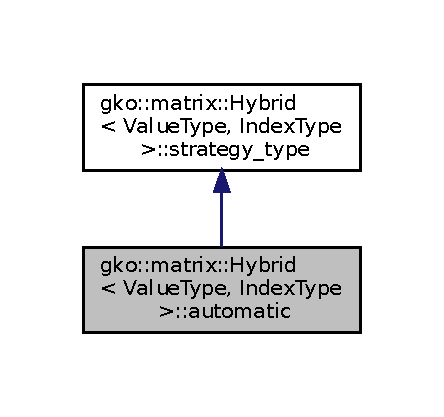
\includegraphics[width=213pt]{classgko_1_1matrix_1_1Hybrid_1_1automatic__coll__graph}
\end{center}
\end{figure}
\doxysubsection*{Public Member Functions}
\begin{DoxyCompactItemize}
\item 
\mbox{\Hypertarget{classgko_1_1matrix_1_1Hybrid_1_1automatic_aadf787a2d56fe0e67c4108f14ee0cb6e}\label{classgko_1_1matrix_1_1Hybrid_1_1automatic_aadf787a2d56fe0e67c4108f14ee0cb6e}} 
\mbox{\hyperlink{classgko_1_1matrix_1_1Hybrid_1_1automatic_aadf787a2d56fe0e67c4108f14ee0cb6e}{automatic}} ()
\begin{DoxyCompactList}\small\item\em Creates an automatic strategy. \end{DoxyCompactList}\item 
\mbox{\hyperlink{namespacegko_a6e5c95df0ae4e47aab2f604a22d98ee7}{size\+\_\+type}} \mbox{\hyperlink{classgko_1_1matrix_1_1Hybrid_1_1automatic_a804d556fbcbe8ed754e167f270b16118}{compute\+\_\+ell\+\_\+num\+\_\+stored\+\_\+elements\+\_\+per\+\_\+row}} (\mbox{\hyperlink{classgko_1_1Array}{Array}}$<$ \mbox{\hyperlink{namespacegko_a6e5c95df0ae4e47aab2f604a22d98ee7}{size\+\_\+type}} $>$ $\ast$row\+\_\+nnz) const override
\begin{DoxyCompactList}\small\item\em Computes the number of stored elements per row of the ell part. \end{DoxyCompactList}\end{DoxyCompactItemize}


\doxysubsection{Detailed Description}
\subsubsection*{template$<$typename Value\+Type = default\+\_\+precision, typename Index\+Type = int32$>$\newline
class gko\+::matrix\+::\+Hybrid$<$ Value\+Type, Index\+Type $>$\+::automatic}

automatic is a \mbox{\hyperlink{classgko_1_1matrix_1_1Hybrid_1_1strategy__type}{strategy\+\_\+type}} which decides the number of stored elements per row of the ell part automatically. 

\doxysubsection{Member Function Documentation}
\mbox{\Hypertarget{classgko_1_1matrix_1_1Hybrid_1_1automatic_a804d556fbcbe8ed754e167f270b16118}\label{classgko_1_1matrix_1_1Hybrid_1_1automatic_a804d556fbcbe8ed754e167f270b16118}} 
\index{gko::matrix::Hybrid$<$ ValueType, IndexType $>$::automatic@{gko::matrix::Hybrid$<$ ValueType, IndexType $>$::automatic}!compute\_ell\_num\_stored\_elements\_per\_row@{compute\_ell\_num\_stored\_elements\_per\_row}}
\index{compute\_ell\_num\_stored\_elements\_per\_row@{compute\_ell\_num\_stored\_elements\_per\_row}!gko::matrix::Hybrid$<$ ValueType, IndexType $>$::automatic@{gko::matrix::Hybrid$<$ ValueType, IndexType $>$::automatic}}
\doxysubsubsection{\texorpdfstring{compute\_ell\_num\_stored\_elements\_per\_row()}{compute\_ell\_num\_stored\_elements\_per\_row()}}
{\footnotesize\ttfamily template$<$typename Value\+Type = default\+\_\+precision, typename Index\+Type = int32$>$ \\
\mbox{\hyperlink{namespacegko_a6e5c95df0ae4e47aab2f604a22d98ee7}{size\+\_\+type}} \mbox{\hyperlink{classgko_1_1matrix_1_1Hybrid}{gko\+::matrix\+::\+Hybrid}}$<$ Value\+Type, Index\+Type $>$\+::automatic\+::compute\+\_\+ell\+\_\+num\+\_\+stored\+\_\+elements\+\_\+per\+\_\+row (\begin{DoxyParamCaption}\item[{\mbox{\hyperlink{classgko_1_1Array}{Array}}$<$ \mbox{\hyperlink{namespacegko_a6e5c95df0ae4e47aab2f604a22d98ee7}{size\+\_\+type}} $>$ $\ast$}]{row\+\_\+nnz }\end{DoxyParamCaption}) const\hspace{0.3cm}{\ttfamily [inline]}, {\ttfamily [override]}, {\ttfamily [virtual]}}



Computes the number of stored elements per row of the ell part. 


\begin{DoxyParams}{Parameters}
{\em row\+\_\+nnz} & the number of nonzeros of each row\\
\hline
\end{DoxyParams}
\begin{DoxyReturn}{Returns}
the number of stored elements per row of the ell part 
\end{DoxyReturn}


Implements \mbox{\hyperlink{classgko_1_1matrix_1_1Hybrid_1_1strategy__type_a0a0cd4024f27c7d0f286f35fc0a6de60}{gko\+::matrix\+::\+Hybrid$<$ Value\+Type, Index\+Type $>$\+::strategy\+\_\+type}}.



References gko\+::matrix\+::\+Hybrid$<$ Value\+Type, Index\+Type $>$\+::imbalance\+\_\+bounded\+\_\+limit\+::compute\+\_\+ell\+\_\+num\+\_\+stored\+\_\+elements\+\_\+per\+\_\+row().



The documentation for this class was generated from the following file\+:\begin{DoxyCompactItemize}
\item 
ginkgo/core/matrix/hybrid.\+hpp (29444d385)\end{DoxyCompactItemize}

\hypertarget{classgko_1_1matrix_1_1Csr_1_1automatical}{}\doxysection{gko\+::matrix\+::Csr$<$ Value\+Type, Index\+Type $>$\+::automatical Class Reference}
\label{classgko_1_1matrix_1_1Csr_1_1automatical}\index{gko::matrix::Csr$<$ ValueType, IndexType $>$::automatical@{gko::matrix::Csr$<$ ValueType, IndexType $>$::automatical}}


Collaboration diagram for gko\+::matrix\+::Csr$<$ Value\+Type, Index\+Type $>$\+::automatical\+:
\nopagebreak
\begin{figure}[H]
\begin{center}
\leavevmode
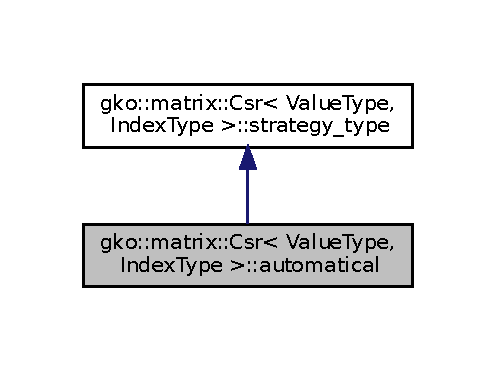
\includegraphics[width=238pt]{classgko_1_1matrix_1_1Csr_1_1automatical__coll__graph}
\end{center}
\end{figure}
\doxysubsection*{Public Member Functions}
\begin{DoxyCompactItemize}
\item 
\mbox{\Hypertarget{classgko_1_1matrix_1_1Csr_1_1automatical_a4ba9ec73abf4ac52d00811065d50b6d9}\label{classgko_1_1matrix_1_1Csr_1_1automatical_a4ba9ec73abf4ac52d00811065d50b6d9}} 
\mbox{\hyperlink{classgko_1_1matrix_1_1Csr_1_1automatical_a4ba9ec73abf4ac52d00811065d50b6d9}{automatical}} ()
\begin{DoxyCompactList}\small\item\em Creates an automatical strategy. \end{DoxyCompactList}\item 
\mbox{\hyperlink{classgko_1_1matrix_1_1Csr_1_1automatical_a5e3cff9dc55b22b01ddf3db31731b267}{automatical}} (std\+::shared\+\_\+ptr$<$ const \mbox{\hyperlink{classgko_1_1CudaExecutor}{Cuda\+Executor}} $>$ exec)
\begin{DoxyCompactList}\small\item\em Creates an automatical strategy with C\+U\+DA executor. \end{DoxyCompactList}\item 
\mbox{\hyperlink{classgko_1_1matrix_1_1Csr_1_1automatical_a9ec5b221681ed8e5f33fd77c9b781690}{automatical}} (std\+::shared\+\_\+ptr$<$ const \mbox{\hyperlink{classgko_1_1HipExecutor}{Hip\+Executor}} $>$ exec)
\begin{DoxyCompactList}\small\item\em Creates an automatical strategy with H\+IP executor. \end{DoxyCompactList}\item 
\mbox{\hyperlink{classgko_1_1matrix_1_1Csr_1_1automatical_aded15aecba0706d609e7557a585a686a}{automatical}} (int64\+\_\+t nwarps, int warp\+\_\+size=32, bool cuda\+\_\+strategy=true)
\begin{DoxyCompactList}\small\item\em Creates an automatical strategy with specified parameters. \end{DoxyCompactList}\item 
void \mbox{\hyperlink{classgko_1_1matrix_1_1Csr_1_1automatical_aefa241047539f2ee7784a54cf5051720}{process}} (const \mbox{\hyperlink{classgko_1_1Array}{Array}}$<$ index\+\_\+type $>$ \&mtx\+\_\+row\+\_\+ptrs, \mbox{\hyperlink{classgko_1_1Array}{Array}}$<$ index\+\_\+type $>$ $\ast$mtx\+\_\+srow) override
\begin{DoxyCompactList}\small\item\em Computes srow according to row pointers. \end{DoxyCompactList}\item 
int64\+\_\+t \mbox{\hyperlink{classgko_1_1matrix_1_1Csr_1_1automatical_a4c3e6ae322c261f0da10641c58e83398}{clac\+\_\+size}} (const int64\+\_\+t nnz) override
\begin{DoxyCompactList}\small\item\em Computes the srow size according to the number of nonzeros. \end{DoxyCompactList}\item 
\mbox{\Hypertarget{classgko_1_1matrix_1_1Csr_1_1automatical_a593dee0b8e70a753670e1d81a05d2307}\label{classgko_1_1matrix_1_1Csr_1_1automatical_a593dee0b8e70a753670e1d81a05d2307}} 
index\+\_\+type {\bfseries get\+\_\+max\+\_\+length\+\_\+per\+\_\+row} () const noexcept
\item 
std\+::shared\+\_\+ptr$<$ \mbox{\hyperlink{classgko_1_1matrix_1_1Csr_1_1strategy__type}{strategy\+\_\+type}} $>$ \mbox{\hyperlink{classgko_1_1matrix_1_1Csr_1_1automatical_ae1c938cbb2b6d0609eee055febb2fbd2}{copy}} () override
\begin{DoxyCompactList}\small\item\em Copy a strategy. \end{DoxyCompactList}\end{DoxyCompactItemize}
\doxysubsection*{Public Attributes}
\begin{DoxyCompactItemize}
\item 
\mbox{\Hypertarget{classgko_1_1matrix_1_1Csr_1_1automatical_a909abe5ebd5bb68031b7ab68c2f847d4}\label{classgko_1_1matrix_1_1Csr_1_1automatical_a909abe5ebd5bb68031b7ab68c2f847d4}} 
const index\+\_\+type {\bfseries nvidia\+\_\+row\+\_\+len\+\_\+limit} = 1024
\item 
\mbox{\Hypertarget{classgko_1_1matrix_1_1Csr_1_1automatical_ac1f75409470cd36a437d76a2bc4e79fd}\label{classgko_1_1matrix_1_1Csr_1_1automatical_ac1f75409470cd36a437d76a2bc4e79fd}} 
const index\+\_\+type {\bfseries nvidia\+\_\+nnz\+\_\+limit} = 1e6
\item 
\mbox{\Hypertarget{classgko_1_1matrix_1_1Csr_1_1automatical_a21ff9463860ca7269f16f5cee771d999}\label{classgko_1_1matrix_1_1Csr_1_1automatical_a21ff9463860ca7269f16f5cee771d999}} 
const index\+\_\+type {\bfseries amd\+\_\+row\+\_\+len\+\_\+limit} = 768
\item 
\mbox{\Hypertarget{classgko_1_1matrix_1_1Csr_1_1automatical_a2cdf9df0edbbaff89c3bb7e5979953c7}\label{classgko_1_1matrix_1_1Csr_1_1automatical_a2cdf9df0edbbaff89c3bb7e5979953c7}} 
const index\+\_\+type {\bfseries amd\+\_\+nnz\+\_\+limit} = 1e8
\end{DoxyCompactItemize}


\doxysubsection{Constructor \& Destructor Documentation}
\mbox{\Hypertarget{classgko_1_1matrix_1_1Csr_1_1automatical_a5e3cff9dc55b22b01ddf3db31731b267}\label{classgko_1_1matrix_1_1Csr_1_1automatical_a5e3cff9dc55b22b01ddf3db31731b267}} 
\index{gko::matrix::Csr$<$ ValueType, IndexType $>$::automatical@{gko::matrix::Csr$<$ ValueType, IndexType $>$::automatical}!automatical@{automatical}}
\index{automatical@{automatical}!gko::matrix::Csr$<$ ValueType, IndexType $>$::automatical@{gko::matrix::Csr$<$ ValueType, IndexType $>$::automatical}}
\doxysubsubsection{\texorpdfstring{automatical()}{automatical()}\hspace{0.1cm}{\footnotesize\ttfamily [1/3]}}
{\footnotesize\ttfamily template$<$typename Value\+Type = default\+\_\+precision, typename Index\+Type = int32$>$ \\
\mbox{\hyperlink{classgko_1_1matrix_1_1Csr}{gko\+::matrix\+::\+Csr}}$<$ Value\+Type, Index\+Type $>$\+::automatical\+::automatical (\begin{DoxyParamCaption}\item[{std\+::shared\+\_\+ptr$<$ const \mbox{\hyperlink{classgko_1_1CudaExecutor}{Cuda\+Executor}} $>$}]{exec }\end{DoxyParamCaption})\hspace{0.3cm}{\ttfamily [inline]}}



Creates an automatical strategy with C\+U\+DA executor. 


\begin{DoxyParams}{Parameters}
{\em exec} & the C\+U\+DA executor \\
\hline
\end{DoxyParams}
\mbox{\Hypertarget{classgko_1_1matrix_1_1Csr_1_1automatical_a9ec5b221681ed8e5f33fd77c9b781690}\label{classgko_1_1matrix_1_1Csr_1_1automatical_a9ec5b221681ed8e5f33fd77c9b781690}} 
\index{gko::matrix::Csr$<$ ValueType, IndexType $>$::automatical@{gko::matrix::Csr$<$ ValueType, IndexType $>$::automatical}!automatical@{automatical}}
\index{automatical@{automatical}!gko::matrix::Csr$<$ ValueType, IndexType $>$::automatical@{gko::matrix::Csr$<$ ValueType, IndexType $>$::automatical}}
\doxysubsubsection{\texorpdfstring{automatical()}{automatical()}\hspace{0.1cm}{\footnotesize\ttfamily [2/3]}}
{\footnotesize\ttfamily template$<$typename Value\+Type = default\+\_\+precision, typename Index\+Type = int32$>$ \\
\mbox{\hyperlink{classgko_1_1matrix_1_1Csr}{gko\+::matrix\+::\+Csr}}$<$ Value\+Type, Index\+Type $>$\+::automatical\+::automatical (\begin{DoxyParamCaption}\item[{std\+::shared\+\_\+ptr$<$ const \mbox{\hyperlink{classgko_1_1HipExecutor}{Hip\+Executor}} $>$}]{exec }\end{DoxyParamCaption})\hspace{0.3cm}{\ttfamily [inline]}}



Creates an automatical strategy with H\+IP executor. 


\begin{DoxyParams}{Parameters}
{\em exec} & the H\+IP executor \\
\hline
\end{DoxyParams}
\mbox{\Hypertarget{classgko_1_1matrix_1_1Csr_1_1automatical_aded15aecba0706d609e7557a585a686a}\label{classgko_1_1matrix_1_1Csr_1_1automatical_aded15aecba0706d609e7557a585a686a}} 
\index{gko::matrix::Csr$<$ ValueType, IndexType $>$::automatical@{gko::matrix::Csr$<$ ValueType, IndexType $>$::automatical}!automatical@{automatical}}
\index{automatical@{automatical}!gko::matrix::Csr$<$ ValueType, IndexType $>$::automatical@{gko::matrix::Csr$<$ ValueType, IndexType $>$::automatical}}
\doxysubsubsection{\texorpdfstring{automatical()}{automatical()}\hspace{0.1cm}{\footnotesize\ttfamily [3/3]}}
{\footnotesize\ttfamily template$<$typename Value\+Type = default\+\_\+precision, typename Index\+Type = int32$>$ \\
\mbox{\hyperlink{classgko_1_1matrix_1_1Csr}{gko\+::matrix\+::\+Csr}}$<$ Value\+Type, Index\+Type $>$\+::automatical\+::automatical (\begin{DoxyParamCaption}\item[{int64\+\_\+t}]{nwarps,  }\item[{int}]{warp\+\_\+size = {\ttfamily 32},  }\item[{bool}]{cuda\+\_\+strategy = {\ttfamily true} }\end{DoxyParamCaption})\hspace{0.3cm}{\ttfamily [inline]}}



Creates an automatical strategy with specified parameters. 


\begin{DoxyParams}{Parameters}
{\em nwarps} & the number of warps in the executor \\
\hline
{\em warp\+\_\+size} & the warp size of the executor \\
\hline
{\em cuda\+\_\+strategy} & whether the {\ttfamily cuda\+\_\+strategy} needs to be used.\\
\hline
\end{DoxyParams}
\begin{DoxyNote}{Note}
The warp\+\_\+size must be the size of full warp. When using this constructor, set\+\_\+strategy needs to be called with correct parameters which is replaced during the conversion. 
\end{DoxyNote}


\doxysubsection{Member Function Documentation}
\mbox{\Hypertarget{classgko_1_1matrix_1_1Csr_1_1automatical_a4c3e6ae322c261f0da10641c58e83398}\label{classgko_1_1matrix_1_1Csr_1_1automatical_a4c3e6ae322c261f0da10641c58e83398}} 
\index{gko::matrix::Csr$<$ ValueType, IndexType $>$::automatical@{gko::matrix::Csr$<$ ValueType, IndexType $>$::automatical}!clac\_size@{clac\_size}}
\index{clac\_size@{clac\_size}!gko::matrix::Csr$<$ ValueType, IndexType $>$::automatical@{gko::matrix::Csr$<$ ValueType, IndexType $>$::automatical}}
\doxysubsubsection{\texorpdfstring{clac\_size()}{clac\_size()}}
{\footnotesize\ttfamily template$<$typename Value\+Type = default\+\_\+precision, typename Index\+Type = int32$>$ \\
int64\+\_\+t \mbox{\hyperlink{classgko_1_1matrix_1_1Csr}{gko\+::matrix\+::\+Csr}}$<$ Value\+Type, Index\+Type $>$\+::automatical\+::clac\+\_\+size (\begin{DoxyParamCaption}\item[{const int64\+\_\+t}]{nnz }\end{DoxyParamCaption})\hspace{0.3cm}{\ttfamily [inline]}, {\ttfamily [override]}, {\ttfamily [virtual]}}



Computes the srow size according to the number of nonzeros. 


\begin{DoxyParams}{Parameters}
{\em nnz} & the number of nonzeros\\
\hline
\end{DoxyParams}
\begin{DoxyReturn}{Returns}
the size of srow 
\end{DoxyReturn}


Implements \mbox{\hyperlink{classgko_1_1matrix_1_1Csr_1_1strategy__type_a07a6dda9dd04ed8abd914f3a69f330f2}{gko\+::matrix\+::\+Csr$<$ Value\+Type, Index\+Type $>$\+::strategy\+\_\+type}}.

\mbox{\Hypertarget{classgko_1_1matrix_1_1Csr_1_1automatical_ae1c938cbb2b6d0609eee055febb2fbd2}\label{classgko_1_1matrix_1_1Csr_1_1automatical_ae1c938cbb2b6d0609eee055febb2fbd2}} 
\index{gko::matrix::Csr$<$ ValueType, IndexType $>$::automatical@{gko::matrix::Csr$<$ ValueType, IndexType $>$::automatical}!copy@{copy}}
\index{copy@{copy}!gko::matrix::Csr$<$ ValueType, IndexType $>$::automatical@{gko::matrix::Csr$<$ ValueType, IndexType $>$::automatical}}
\doxysubsubsection{\texorpdfstring{copy()}{copy()}}
{\footnotesize\ttfamily template$<$typename Value\+Type = default\+\_\+precision, typename Index\+Type = int32$>$ \\
std\+::shared\+\_\+ptr$<$\mbox{\hyperlink{classgko_1_1matrix_1_1Csr_1_1strategy__type}{strategy\+\_\+type}}$>$ \mbox{\hyperlink{classgko_1_1matrix_1_1Csr}{gko\+::matrix\+::\+Csr}}$<$ Value\+Type, Index\+Type $>$\+::automatical\+::copy (\begin{DoxyParamCaption}{ }\end{DoxyParamCaption})\hspace{0.3cm}{\ttfamily [inline]}, {\ttfamily [override]}, {\ttfamily [virtual]}}



Copy a strategy. 

This is a workaround until strategies are revamped, since strategies like {\ttfamily automatical} do not work when actually shared. 

Implements \mbox{\hyperlink{classgko_1_1matrix_1_1Csr_1_1strategy__type_adf3dc78938ffb991608b272447db6a68}{gko\+::matrix\+::\+Csr$<$ Value\+Type, Index\+Type $>$\+::strategy\+\_\+type}}.

\mbox{\Hypertarget{classgko_1_1matrix_1_1Csr_1_1automatical_aefa241047539f2ee7784a54cf5051720}\label{classgko_1_1matrix_1_1Csr_1_1automatical_aefa241047539f2ee7784a54cf5051720}} 
\index{gko::matrix::Csr$<$ ValueType, IndexType $>$::automatical@{gko::matrix::Csr$<$ ValueType, IndexType $>$::automatical}!process@{process}}
\index{process@{process}!gko::matrix::Csr$<$ ValueType, IndexType $>$::automatical@{gko::matrix::Csr$<$ ValueType, IndexType $>$::automatical}}
\doxysubsubsection{\texorpdfstring{process()}{process()}}
{\footnotesize\ttfamily template$<$typename Value\+Type = default\+\_\+precision, typename Index\+Type = int32$>$ \\
void \mbox{\hyperlink{classgko_1_1matrix_1_1Csr}{gko\+::matrix\+::\+Csr}}$<$ Value\+Type, Index\+Type $>$\+::automatical\+::process (\begin{DoxyParamCaption}\item[{const \mbox{\hyperlink{classgko_1_1Array}{Array}}$<$ index\+\_\+type $>$ \&}]{mtx\+\_\+row\+\_\+ptrs,  }\item[{\mbox{\hyperlink{classgko_1_1Array}{Array}}$<$ index\+\_\+type $>$ $\ast$}]{mtx\+\_\+srow }\end{DoxyParamCaption})\hspace{0.3cm}{\ttfamily [inline]}, {\ttfamily [override]}, {\ttfamily [virtual]}}



Computes srow according to row pointers. 


\begin{DoxyParams}{Parameters}
{\em mtx\+\_\+row\+\_\+ptrs} & the row pointers of the matrix \\
\hline
{\em mtx\+\_\+srow} & the srow of the matrix \\
\hline
\end{DoxyParams}


Implements \mbox{\hyperlink{classgko_1_1matrix_1_1Csr_1_1strategy__type_a58bda9208766e57d861262d4059b65b4}{gko\+::matrix\+::\+Csr$<$ Value\+Type, Index\+Type $>$\+::strategy\+\_\+type}}.



References gko\+::\+Array$<$ Value\+Type $>$\+::get\+\_\+const\+\_\+data(), gko\+::\+Array$<$ Value\+Type $>$\+::get\+\_\+executor(), gko\+::matrix\+::\+Csr$<$ Value\+Type, Index\+Type $>$\+::strategy\+\_\+type\+::get\+\_\+name(), gko\+::\+Array$<$ Value\+Type $>$\+::get\+\_\+num\+\_\+elems(), gko\+::max(), gko\+::matrix\+::\+Csr$<$ Value\+Type, Index\+Type $>$\+::classical\+::process(), and gko\+::matrix\+::\+Csr$<$ Value\+Type, Index\+Type $>$\+::load\+\_\+balance\+::process().



The documentation for this class was generated from the following file\+:\begin{DoxyCompactItemize}
\item 
ginkgo/core/matrix/csr.\+hpp (7f07c6d04)\end{DoxyCompactItemize}

\hypertarget{classgko_1_1solver_1_1Bicgstab}{}\doxysection{gko\+::solver\+::Bicgstab$<$ Value\+Type $>$ Class Template Reference}
\label{classgko_1_1solver_1_1Bicgstab}\index{gko::solver::Bicgstab$<$ ValueType $>$@{gko::solver::Bicgstab$<$ ValueType $>$}}


Bi\+C\+G\+S\+T\+AB or the Bi-\/\+Conjugate Gradient-\/\+Stabilized is a Krylov subspace solver.  




{\ttfamily \#include $<$ginkgo/core/solver/bicgstab.\+hpp$>$}



Collaboration diagram for gko\+::solver\+::Bicgstab$<$ Value\+Type $>$\+:
\nopagebreak
\begin{figure}[H]
\begin{center}
\leavevmode
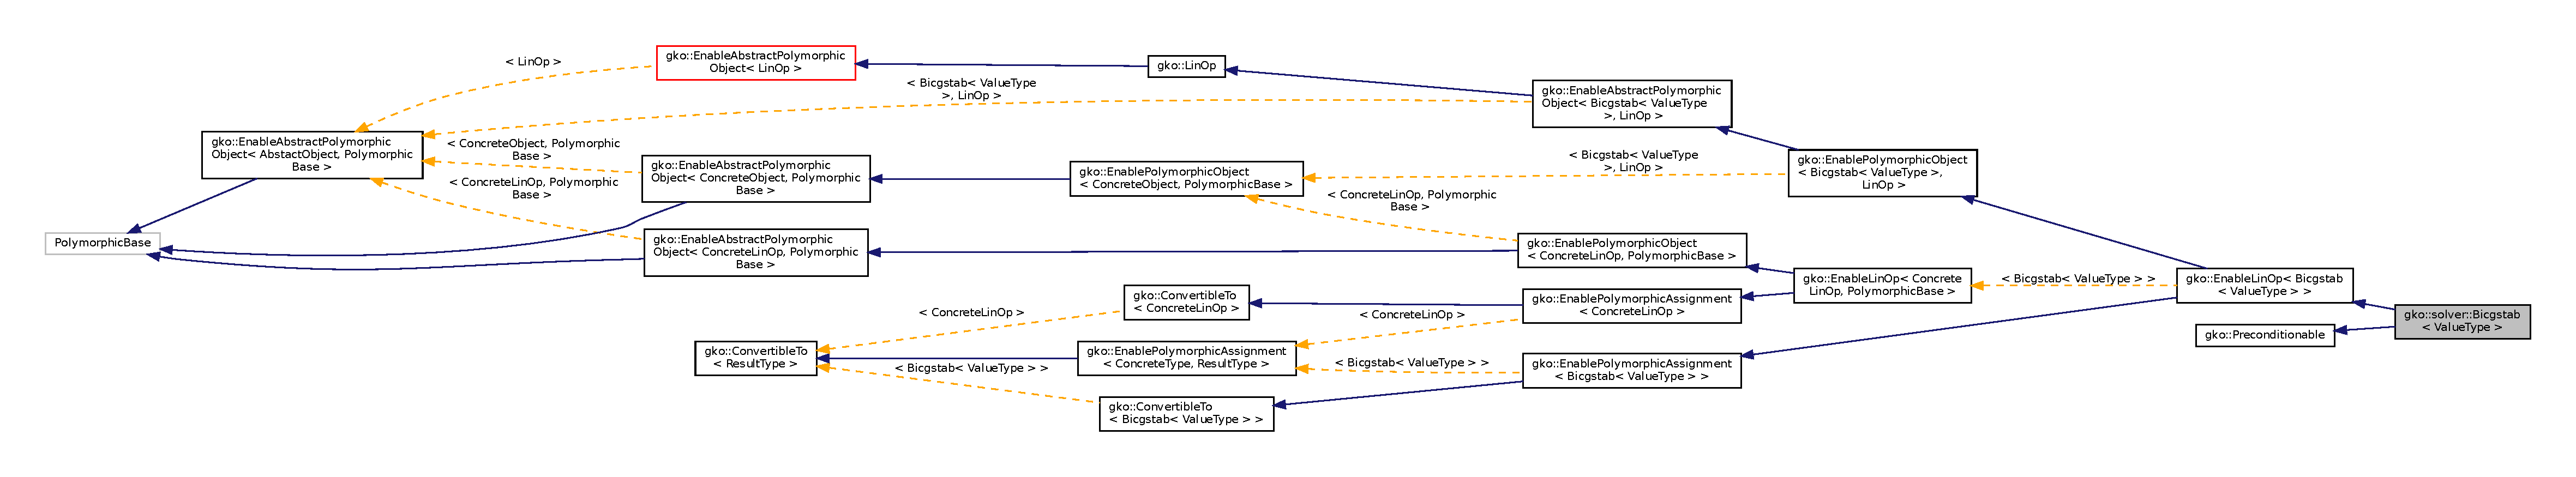
\includegraphics[width=350pt]{classgko_1_1solver_1_1Bicgstab__coll__graph}
\end{center}
\end{figure}
\doxysubsection*{Classes}
\begin{DoxyCompactItemize}
\item 
class \mbox{\hyperlink{classgko_1_1solver_1_1Bicgstab_1_1Factory}{Factory}}
\item 
struct \mbox{\hyperlink{structgko_1_1solver_1_1Bicgstab_1_1parameters__type}{parameters\+\_\+type}}
\end{DoxyCompactItemize}
\doxysubsection*{Public Types}
\begin{DoxyCompactItemize}
\item 
\mbox{\Hypertarget{classgko_1_1solver_1_1Bicgstab_ab670b7a800a5b86f4733adfe314a67a7}\label{classgko_1_1solver_1_1Bicgstab_ab670b7a800a5b86f4733adfe314a67a7}} 
using {\bfseries value\+\_\+type} = Value\+Type
\end{DoxyCompactItemize}
\doxysubsection*{Public Member Functions}
\begin{DoxyCompactItemize}
\item 
std\+::shared\+\_\+ptr$<$ const \mbox{\hyperlink{classgko_1_1LinOp}{Lin\+Op}} $>$ \mbox{\hyperlink{classgko_1_1solver_1_1Bicgstab_ada73e8ca3e8924011c8780cab92f651e}{get\+\_\+system\+\_\+matrix}} () const
\begin{DoxyCompactList}\small\item\em Gets the system operator (matrix) of the linear system. \end{DoxyCompactList}\item 
\mbox{\Hypertarget{classgko_1_1solver_1_1Bicgstab_ad9f55802a39cbf339c400f3a5eeb7a4a}\label{classgko_1_1solver_1_1Bicgstab_ad9f55802a39cbf339c400f3a5eeb7a4a}} 
const \mbox{\hyperlink{structgko_1_1solver_1_1Bicgstab_1_1parameters__type}{parameters\+\_\+type}} \& {\bfseries get\+\_\+parameters} () const
\end{DoxyCompactItemize}
\doxysubsection*{Static Public Member Functions}
\begin{DoxyCompactItemize}
\item 
\mbox{\Hypertarget{classgko_1_1solver_1_1Bicgstab_abf0ea911ffb1bd2736dfd9ebfaa46a38}\label{classgko_1_1solver_1_1Bicgstab_abf0ea911ffb1bd2736dfd9ebfaa46a38}} 
static auto {\bfseries build} () -\/$>$ decltype(\mbox{\hyperlink{classgko_1_1solver_1_1Bicgstab_1_1Factory}{Factory}} \+::create())
\end{DoxyCompactItemize}
\doxysubsection*{Friends}
\begin{DoxyCompactItemize}
\item 
\mbox{\Hypertarget{classgko_1_1solver_1_1Bicgstab_ab135a56fe121f9011363f034f1cd292e}\label{classgko_1_1solver_1_1Bicgstab_ab135a56fe121f9011363f034f1cd292e}} 
class {\bfseries Enable\+Lin\+Op$<$ Bicgstab $>$}
\item 
\mbox{\Hypertarget{classgko_1_1solver_1_1Bicgstab_acd2682c6fc5c060a57df8f9cfad990b5}\label{classgko_1_1solver_1_1Bicgstab_acd2682c6fc5c060a57df8f9cfad990b5}} 
class {\bfseries Enable\+Polymorphic\+Object$<$ Bicgstab, Lin\+Op $>$}
\end{DoxyCompactItemize}


\doxysubsection{Detailed Description}
\subsubsection*{template$<$typename Value\+Type = default\+\_\+precision$>$\newline
class gko\+::solver\+::\+Bicgstab$<$ Value\+Type $>$}

Bi\+C\+G\+S\+T\+AB or the Bi-\/\+Conjugate Gradient-\/\+Stabilized is a Krylov subspace solver. 

Being a generic solver, it is capable of solving general matrices, including non-\/s.\+p.\+d matrices. Though, the memory and the computational requirement of the Bi\+C\+G\+S\+T\+AB solver are higher than of its s.\+p.\+d solver counterpart, it has the capability to solve generic systems. It was developed by stabilizing the Bi\+CG method.


\begin{DoxyTemplParams}{Template Parameters}
{\em Value\+Type} & precision of the elements of the system matrix. \\
\hline
\end{DoxyTemplParams}


\doxysubsection{Member Function Documentation}
\mbox{\Hypertarget{classgko_1_1solver_1_1Bicgstab_ada73e8ca3e8924011c8780cab92f651e}\label{classgko_1_1solver_1_1Bicgstab_ada73e8ca3e8924011c8780cab92f651e}} 
\index{gko::solver::Bicgstab$<$ ValueType $>$@{gko::solver::Bicgstab$<$ ValueType $>$}!get\_system\_matrix@{get\_system\_matrix}}
\index{get\_system\_matrix@{get\_system\_matrix}!gko::solver::Bicgstab$<$ ValueType $>$@{gko::solver::Bicgstab$<$ ValueType $>$}}
\doxysubsubsection{\texorpdfstring{get\_system\_matrix()}{get\_system\_matrix()}}
{\footnotesize\ttfamily template$<$typename Value\+Type  = default\+\_\+precision$>$ \\
std\+::shared\+\_\+ptr$<$const \mbox{\hyperlink{classgko_1_1LinOp}{Lin\+Op}}$>$ \mbox{\hyperlink{classgko_1_1solver_1_1Bicgstab}{gko\+::solver\+::\+Bicgstab}}$<$ Value\+Type $>$\+::get\+\_\+system\+\_\+matrix (\begin{DoxyParamCaption}{ }\end{DoxyParamCaption}) const\hspace{0.3cm}{\ttfamily [inline]}}



Gets the system operator (matrix) of the linear system. 

\begin{DoxyReturn}{Returns}
the system operator (matrix) 
\end{DoxyReturn}


The documentation for this class was generated from the following file\+:\begin{DoxyCompactItemize}
\item 
ginkgo/core/solver/bicgstab.\+hpp (c380ba800)\end{DoxyCompactItemize}

\hypertarget{structgko_1_1accessor_1_1bitwise__and}{}\doxysection{gko\+::accessor\+::bitwise\+\_\+and$<$ Kind, First\+Operand, Second\+Operand $>$ Struct Template Reference}
\label{structgko_1_1accessor_1_1bitwise__and}\index{gko::accessor::bitwise\_and$<$ Kind, FirstOperand, SecondOperand $>$@{gko::accessor::bitwise\_and$<$ Kind, FirstOperand, SecondOperand $>$}}


Collaboration diagram for gko\+::accessor\+::bitwise\+\_\+and$<$ Kind, First\+Operand, Second\+Operand $>$\+:
\nopagebreak
\begin{figure}[H]
\begin{center}
\leavevmode
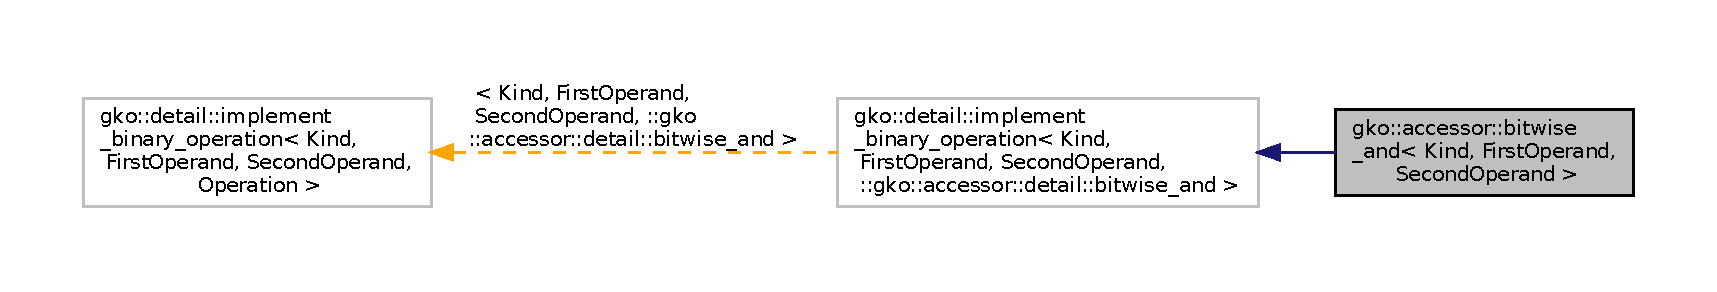
\includegraphics[width=350pt]{structgko_1_1accessor_1_1bitwise__and__coll__graph}
\end{center}
\end{figure}


The documentation for this struct was generated from the following file\+:\begin{DoxyCompactItemize}
\item 
ginkgo/core/base/range.\+hpp\end{DoxyCompactItemize}

\hypertarget{structgko_1_1accessor_1_1bitwise__not}{}\section{gko\+:\+:accessor\+:\+:bitwise\+\_\+not$<$ Operand $>$ Struct Template Reference}
\label{structgko_1_1accessor_1_1bitwise__not}\index{gko\+::accessor\+::bitwise\+\_\+not$<$ Operand $>$@{gko\+::accessor\+::bitwise\+\_\+not$<$ Operand $>$}}


Collaboration diagram for gko\+:\+:accessor\+:\+:bitwise\+\_\+not$<$ Operand $>$\+:
\nopagebreak
\begin{figure}[H]
\begin{center}
\leavevmode
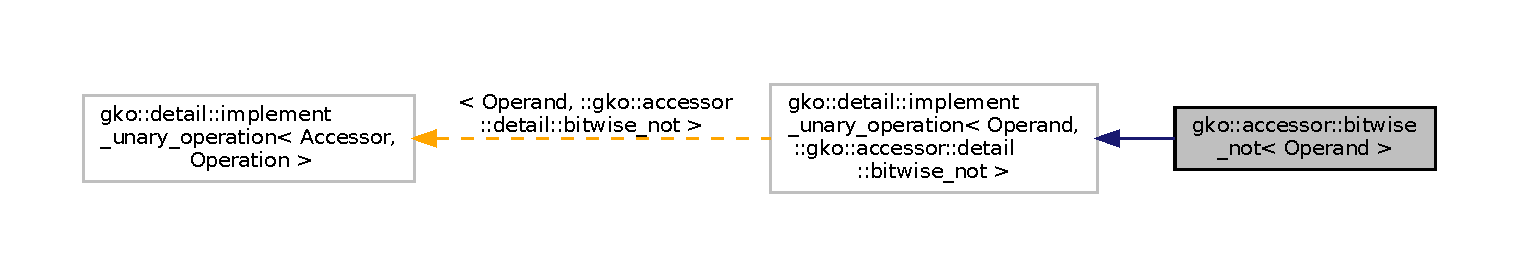
\includegraphics[width=350pt]{structgko_1_1accessor_1_1bitwise__not__coll__graph}
\end{center}
\end{figure}


The documentation for this struct was generated from the following file\+:\begin{DoxyCompactItemize}
\item 
ginkgo/core/base/range.\+hpp (9f8f3063)\end{DoxyCompactItemize}

\hypertarget{structgko_1_1accessor_1_1bitwise__or}{}\doxysection{gko\+::accessor\+::bitwise\+\_\+or$<$ Kind, First\+Operand, Second\+Operand $>$ Struct Template Reference}
\label{structgko_1_1accessor_1_1bitwise__or}\index{gko::accessor::bitwise\_or$<$ Kind, FirstOperand, SecondOperand $>$@{gko::accessor::bitwise\_or$<$ Kind, FirstOperand, SecondOperand $>$}}


Collaboration diagram for gko\+::accessor\+::bitwise\+\_\+or$<$ Kind, First\+Operand, Second\+Operand $>$\+:
\nopagebreak
\begin{figure}[H]
\begin{center}
\leavevmode
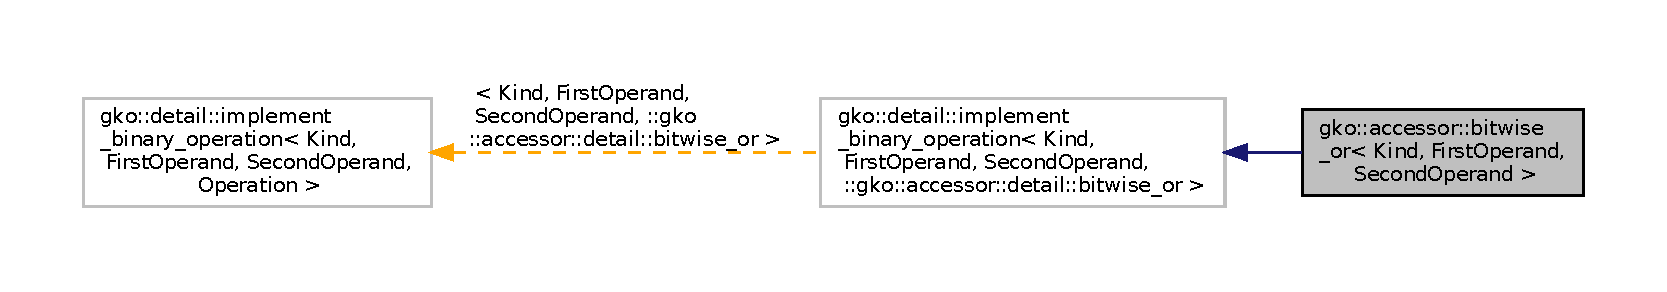
\includegraphics[width=350pt]{structgko_1_1accessor_1_1bitwise__or__coll__graph}
\end{center}
\end{figure}


The documentation for this struct was generated from the following file\+:\begin{DoxyCompactItemize}
\item 
ginkgo/core/base/range.\+hpp (357228f4e)\end{DoxyCompactItemize}

\hypertarget{structgko_1_1accessor_1_1bitwise__xor}{}\section{gko\+:\+:accessor\+:\+:bitwise\+\_\+xor$<$ Kind, First\+Operand, Second\+Operand $>$ Struct Template Reference}
\label{structgko_1_1accessor_1_1bitwise__xor}\index{gko\+::accessor\+::bitwise\+\_\+xor$<$ Kind, First\+Operand, Second\+Operand $>$@{gko\+::accessor\+::bitwise\+\_\+xor$<$ Kind, First\+Operand, Second\+Operand $>$}}


Collaboration diagram for gko\+:\+:accessor\+:\+:bitwise\+\_\+xor$<$ Kind, First\+Operand, Second\+Operand $>$\+:
\nopagebreak
\begin{figure}[H]
\begin{center}
\leavevmode
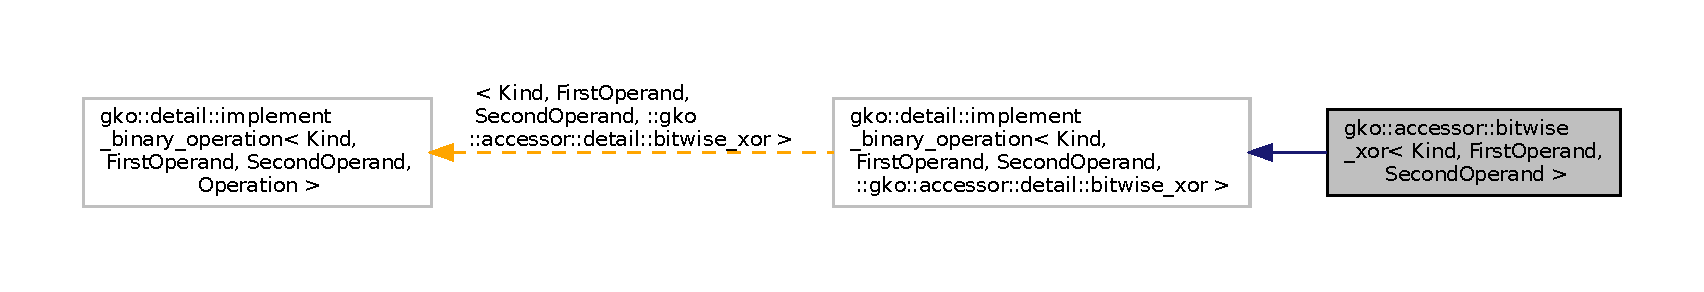
\includegraphics[width=350pt]{structgko_1_1accessor_1_1bitwise__xor__coll__graph}
\end{center}
\end{figure}


The documentation for this struct was generated from the following file\+:\begin{DoxyCompactItemize}
\item 
ginkgo/core/base/range.\+hpp (f1a4eb68)\end{DoxyCompactItemize}

\hypertarget{structgko_1_1preconditioner_1_1block__interleaved__storage__scheme}{}\section{gko\+:\+:preconditioner\+:\+:block\+\_\+interleaved\+\_\+storage\+\_\+scheme$<$ Index\+Type $>$ Struct Template Reference}
\label{structgko_1_1preconditioner_1_1block__interleaved__storage__scheme}\index{gko\+::preconditioner\+::block\+\_\+interleaved\+\_\+storage\+\_\+scheme$<$ Index\+Type $>$@{gko\+::preconditioner\+::block\+\_\+interleaved\+\_\+storage\+\_\+scheme$<$ Index\+Type $>$}}


Defines the parameters of the interleaved block storage scheme used by block-\/\+Jacobi blocks.  




{\ttfamily \#include $<$ginkgo/core/preconditioner/jacobi.\+hpp$>$}



Collaboration diagram for gko\+:\+:preconditioner\+:\+:block\+\_\+interleaved\+\_\+storage\+\_\+scheme$<$ Index\+Type $>$\+:
\nopagebreak
\begin{figure}[H]
\begin{center}
\leavevmode
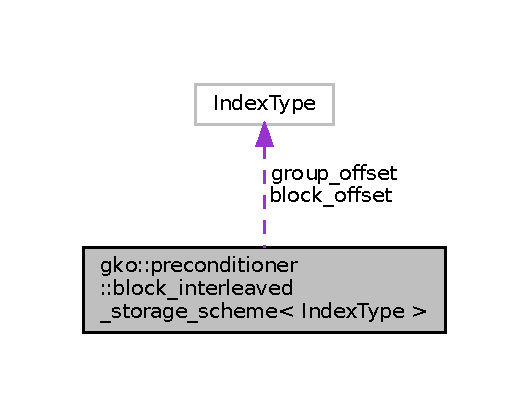
\includegraphics[width=254pt]{structgko_1_1preconditioner_1_1block__interleaved__storage__scheme__coll__graph}
\end{center}
\end{figure}
\subsection*{Public Member Functions}
\begin{DoxyCompactItemize}
\item 
Index\+Type \hyperlink{structgko_1_1preconditioner_1_1block__interleaved__storage__scheme_af5eee19f00b1cd4c378ac3410be72093}{get\+\_\+group\+\_\+size} () const noexcept
\begin{DoxyCompactList}\small\item\em Returns the number of elements in the group. \end{DoxyCompactList}\item 
\hyperlink{namespacegko_a6e5c95df0ae4e47aab2f604a22d98ee7}{size\+\_\+type} \hyperlink{structgko_1_1preconditioner_1_1block__interleaved__storage__scheme_ae46b38432c1e1b87d5743a649f2cfe84}{compute\+\_\+storage\+\_\+space} (\hyperlink{namespacegko_a6e5c95df0ae4e47aab2f604a22d98ee7}{size\+\_\+type} num\+\_\+blocks) const noexcept
\begin{DoxyCompactList}\small\item\em Computes the storage space required for the requested number of blocks. \end{DoxyCompactList}\item 
Index\+Type \hyperlink{structgko_1_1preconditioner_1_1block__interleaved__storage__scheme_a66a04b4dc90547fde872359c78ee22a4}{get\+\_\+group\+\_\+offset} (Index\+Type block\+\_\+id) const noexcept
\begin{DoxyCompactList}\small\item\em Returns the offset of the group belonging to the block with the given ID. \end{DoxyCompactList}\item 
Index\+Type \hyperlink{structgko_1_1preconditioner_1_1block__interleaved__storage__scheme_a6384280dc1ad46fc1589d0b9165fd022}{get\+\_\+block\+\_\+offset} (Index\+Type block\+\_\+id) const noexcept
\begin{DoxyCompactList}\small\item\em Returns the offset of the block with the given ID within its group. \end{DoxyCompactList}\item 
Index\+Type \hyperlink{structgko_1_1preconditioner_1_1block__interleaved__storage__scheme_ad8356b187814609c7d77bd03e025c48f}{get\+\_\+global\+\_\+block\+\_\+offset} (Index\+Type block\+\_\+id) const noexcept
\begin{DoxyCompactList}\small\item\em Returns the offset of the block with the given ID. \end{DoxyCompactList}\item 
Index\+Type \hyperlink{structgko_1_1preconditioner_1_1block__interleaved__storage__scheme_aa07119fbf99fae71b1f9c4f693e14ce4}{get\+\_\+stride} () const noexcept
\begin{DoxyCompactList}\small\item\em Returns the stride between columns of the block. \end{DoxyCompactList}\end{DoxyCompactItemize}
\subsection*{Public Attributes}
\begin{DoxyCompactItemize}
\item 
\mbox{\Hypertarget{structgko_1_1preconditioner_1_1block__interleaved__storage__scheme_ada09b37f171d433cc74818961fc6eccc}\label{structgko_1_1preconditioner_1_1block__interleaved__storage__scheme_ada09b37f171d433cc74818961fc6eccc}} 
Index\+Type \hyperlink{structgko_1_1preconditioner_1_1block__interleaved__storage__scheme_ada09b37f171d433cc74818961fc6eccc}{block\+\_\+offset}
\begin{DoxyCompactList}\small\item\em The offset between consecutive blocks within the group. \end{DoxyCompactList}\item 
\mbox{\Hypertarget{structgko_1_1preconditioner_1_1block__interleaved__storage__scheme_aa8a6723ef709e69bda55eaabaeee582e}\label{structgko_1_1preconditioner_1_1block__interleaved__storage__scheme_aa8a6723ef709e69bda55eaabaeee582e}} 
Index\+Type \hyperlink{structgko_1_1preconditioner_1_1block__interleaved__storage__scheme_aa8a6723ef709e69bda55eaabaeee582e}{group\+\_\+offset}
\begin{DoxyCompactList}\small\item\em The offset between two block groups. \end{DoxyCompactList}\item 
\hyperlink{namespacegko_a318c831e3fe269ba04c6ed8bf5a71073}{uint32} \hyperlink{structgko_1_1preconditioner_1_1block__interleaved__storage__scheme_a8fa279f4178c767bdbf52ef4d7e23ad1}{group\+\_\+power}
\begin{DoxyCompactList}\small\item\em Then base 2 power of the group. \end{DoxyCompactList}\end{DoxyCompactItemize}


\subsection{Detailed Description}
\subsubsection*{template$<$typename Index\+Type$>$\newline
struct gko\+::preconditioner\+::block\+\_\+interleaved\+\_\+storage\+\_\+scheme$<$ Index\+Type $>$}

Defines the parameters of the interleaved block storage scheme used by block-\/\+Jacobi blocks. 


\begin{DoxyTemplParams}{Template Parameters}
{\em Index\+Type} & type used for storing indices of the matrix \\
\hline
\end{DoxyTemplParams}


\subsection{Member Function Documentation}
\mbox{\Hypertarget{structgko_1_1preconditioner_1_1block__interleaved__storage__scheme_ae46b38432c1e1b87d5743a649f2cfe84}\label{structgko_1_1preconditioner_1_1block__interleaved__storage__scheme_ae46b38432c1e1b87d5743a649f2cfe84}} 
\index{gko\+::preconditioner\+::block\+\_\+interleaved\+\_\+storage\+\_\+scheme@{gko\+::preconditioner\+::block\+\_\+interleaved\+\_\+storage\+\_\+scheme}!compute\+\_\+storage\+\_\+space@{compute\+\_\+storage\+\_\+space}}
\index{compute\+\_\+storage\+\_\+space@{compute\+\_\+storage\+\_\+space}!gko\+::preconditioner\+::block\+\_\+interleaved\+\_\+storage\+\_\+scheme@{gko\+::preconditioner\+::block\+\_\+interleaved\+\_\+storage\+\_\+scheme}}
\subsubsection{\texorpdfstring{compute\+\_\+storage\+\_\+space()}{compute\_storage\_space()}}
{\footnotesize\ttfamily template$<$typename Index\+Type$>$ \\
\hyperlink{namespacegko_a6e5c95df0ae4e47aab2f604a22d98ee7}{size\+\_\+type} \hyperlink{structgko_1_1preconditioner_1_1block__interleaved__storage__scheme}{gko\+::preconditioner\+::block\+\_\+interleaved\+\_\+storage\+\_\+scheme}$<$ Index\+Type $>$\+::compute\+\_\+storage\+\_\+space (\begin{DoxyParamCaption}\item[{\hyperlink{namespacegko_a6e5c95df0ae4e47aab2f604a22d98ee7}{size\+\_\+type}}]{num\+\_\+blocks }\end{DoxyParamCaption}) const\hspace{0.3cm}{\ttfamily [inline]}, {\ttfamily [noexcept]}}



Computes the storage space required for the requested number of blocks. 


\begin{DoxyParams}{Parameters}
{\em num\+\_\+blocks} & the total number of blocks that needs to be stored\\
\hline
\end{DoxyParams}
\begin{DoxyReturn}{Returns}
the total memory (as the number of elements) that need to be allocated for the scheme
\end{DoxyReturn}
\begin{DoxyNote}{Note}
To simplify using the method in situations where the number of blocks is not known, for a special input {\ttfamily size\+\_\+type\{\} -\/ 1} the method returns {\ttfamily 0} to avoid overallocation of memory. 
\end{DoxyNote}
\mbox{\Hypertarget{structgko_1_1preconditioner_1_1block__interleaved__storage__scheme_a6384280dc1ad46fc1589d0b9165fd022}\label{structgko_1_1preconditioner_1_1block__interleaved__storage__scheme_a6384280dc1ad46fc1589d0b9165fd022}} 
\index{gko\+::preconditioner\+::block\+\_\+interleaved\+\_\+storage\+\_\+scheme@{gko\+::preconditioner\+::block\+\_\+interleaved\+\_\+storage\+\_\+scheme}!get\+\_\+block\+\_\+offset@{get\+\_\+block\+\_\+offset}}
\index{get\+\_\+block\+\_\+offset@{get\+\_\+block\+\_\+offset}!gko\+::preconditioner\+::block\+\_\+interleaved\+\_\+storage\+\_\+scheme@{gko\+::preconditioner\+::block\+\_\+interleaved\+\_\+storage\+\_\+scheme}}
\subsubsection{\texorpdfstring{get\+\_\+block\+\_\+offset()}{get\_block\_offset()}}
{\footnotesize\ttfamily template$<$typename Index\+Type$>$ \\
Index\+Type \hyperlink{structgko_1_1preconditioner_1_1block__interleaved__storage__scheme}{gko\+::preconditioner\+::block\+\_\+interleaved\+\_\+storage\+\_\+scheme}$<$ Index\+Type $>$\+::get\+\_\+block\+\_\+offset (\begin{DoxyParamCaption}\item[{Index\+Type}]{block\+\_\+id }\end{DoxyParamCaption}) const\hspace{0.3cm}{\ttfamily [inline]}, {\ttfamily [noexcept]}}



Returns the offset of the block with the given ID within its group. 


\begin{DoxyParams}{Parameters}
{\em block\+\_\+id} & the ID of the block\\
\hline
\end{DoxyParams}
\begin{DoxyReturn}{Returns}
the offset of the block with ID {\ttfamily block\+\_\+id} within its group 
\end{DoxyReturn}


Referenced by gko\+::preconditioner\+::block\+\_\+interleaved\+\_\+storage\+\_\+scheme$<$ index\+\_\+type $>$\+::get\+\_\+global\+\_\+block\+\_\+offset().

\mbox{\Hypertarget{structgko_1_1preconditioner_1_1block__interleaved__storage__scheme_ad8356b187814609c7d77bd03e025c48f}\label{structgko_1_1preconditioner_1_1block__interleaved__storage__scheme_ad8356b187814609c7d77bd03e025c48f}} 
\index{gko\+::preconditioner\+::block\+\_\+interleaved\+\_\+storage\+\_\+scheme@{gko\+::preconditioner\+::block\+\_\+interleaved\+\_\+storage\+\_\+scheme}!get\+\_\+global\+\_\+block\+\_\+offset@{get\+\_\+global\+\_\+block\+\_\+offset}}
\index{get\+\_\+global\+\_\+block\+\_\+offset@{get\+\_\+global\+\_\+block\+\_\+offset}!gko\+::preconditioner\+::block\+\_\+interleaved\+\_\+storage\+\_\+scheme@{gko\+::preconditioner\+::block\+\_\+interleaved\+\_\+storage\+\_\+scheme}}
\subsubsection{\texorpdfstring{get\+\_\+global\+\_\+block\+\_\+offset()}{get\_global\_block\_offset()}}
{\footnotesize\ttfamily template$<$typename Index\+Type$>$ \\
Index\+Type \hyperlink{structgko_1_1preconditioner_1_1block__interleaved__storage__scheme}{gko\+::preconditioner\+::block\+\_\+interleaved\+\_\+storage\+\_\+scheme}$<$ Index\+Type $>$\+::get\+\_\+global\+\_\+block\+\_\+offset (\begin{DoxyParamCaption}\item[{Index\+Type}]{block\+\_\+id }\end{DoxyParamCaption}) const\hspace{0.3cm}{\ttfamily [inline]}, {\ttfamily [noexcept]}}



Returns the offset of the block with the given ID. 


\begin{DoxyParams}{Parameters}
{\em block\+\_\+id} & the ID of the block\\
\hline
\end{DoxyParams}
\begin{DoxyReturn}{Returns}
the offset of the block with ID {\ttfamily block\+\_\+id} 
\end{DoxyReturn}
\mbox{\Hypertarget{structgko_1_1preconditioner_1_1block__interleaved__storage__scheme_a66a04b4dc90547fde872359c78ee22a4}\label{structgko_1_1preconditioner_1_1block__interleaved__storage__scheme_a66a04b4dc90547fde872359c78ee22a4}} 
\index{gko\+::preconditioner\+::block\+\_\+interleaved\+\_\+storage\+\_\+scheme@{gko\+::preconditioner\+::block\+\_\+interleaved\+\_\+storage\+\_\+scheme}!get\+\_\+group\+\_\+offset@{get\+\_\+group\+\_\+offset}}
\index{get\+\_\+group\+\_\+offset@{get\+\_\+group\+\_\+offset}!gko\+::preconditioner\+::block\+\_\+interleaved\+\_\+storage\+\_\+scheme@{gko\+::preconditioner\+::block\+\_\+interleaved\+\_\+storage\+\_\+scheme}}
\subsubsection{\texorpdfstring{get\+\_\+group\+\_\+offset()}{get\_group\_offset()}}
{\footnotesize\ttfamily template$<$typename Index\+Type$>$ \\
Index\+Type \hyperlink{structgko_1_1preconditioner_1_1block__interleaved__storage__scheme}{gko\+::preconditioner\+::block\+\_\+interleaved\+\_\+storage\+\_\+scheme}$<$ Index\+Type $>$\+::get\+\_\+group\+\_\+offset (\begin{DoxyParamCaption}\item[{Index\+Type}]{block\+\_\+id }\end{DoxyParamCaption}) const\hspace{0.3cm}{\ttfamily [inline]}, {\ttfamily [noexcept]}}



Returns the offset of the group belonging to the block with the given ID. 


\begin{DoxyParams}{Parameters}
{\em block\+\_\+id} & the ID of the block\\
\hline
\end{DoxyParams}
\begin{DoxyReturn}{Returns}
the offset of the group belonging to block with ID {\ttfamily block\+\_\+id} 
\end{DoxyReturn}


Referenced by gko\+::preconditioner\+::block\+\_\+interleaved\+\_\+storage\+\_\+scheme$<$ index\+\_\+type $>$\+::get\+\_\+global\+\_\+block\+\_\+offset().

\mbox{\Hypertarget{structgko_1_1preconditioner_1_1block__interleaved__storage__scheme_af5eee19f00b1cd4c378ac3410be72093}\label{structgko_1_1preconditioner_1_1block__interleaved__storage__scheme_af5eee19f00b1cd4c378ac3410be72093}} 
\index{gko\+::preconditioner\+::block\+\_\+interleaved\+\_\+storage\+\_\+scheme@{gko\+::preconditioner\+::block\+\_\+interleaved\+\_\+storage\+\_\+scheme}!get\+\_\+group\+\_\+size@{get\+\_\+group\+\_\+size}}
\index{get\+\_\+group\+\_\+size@{get\+\_\+group\+\_\+size}!gko\+::preconditioner\+::block\+\_\+interleaved\+\_\+storage\+\_\+scheme@{gko\+::preconditioner\+::block\+\_\+interleaved\+\_\+storage\+\_\+scheme}}
\subsubsection{\texorpdfstring{get\+\_\+group\+\_\+size()}{get\_group\_size()}}
{\footnotesize\ttfamily template$<$typename Index\+Type$>$ \\
Index\+Type \hyperlink{structgko_1_1preconditioner_1_1block__interleaved__storage__scheme}{gko\+::preconditioner\+::block\+\_\+interleaved\+\_\+storage\+\_\+scheme}$<$ Index\+Type $>$\+::get\+\_\+group\+\_\+size (\begin{DoxyParamCaption}{ }\end{DoxyParamCaption}) const\hspace{0.3cm}{\ttfamily [inline]}, {\ttfamily [noexcept]}}



Returns the number of elements in the group. 

\begin{DoxyReturn}{Returns}
the number of elements in the group 
\end{DoxyReturn}


Referenced by gko\+::preconditioner\+::block\+\_\+interleaved\+\_\+storage\+\_\+scheme$<$ index\+\_\+type $>$\+::compute\+\_\+storage\+\_\+space(), and gko\+::preconditioner\+::block\+\_\+interleaved\+\_\+storage\+\_\+scheme$<$ index\+\_\+type $>$\+::get\+\_\+block\+\_\+offset().

\mbox{\Hypertarget{structgko_1_1preconditioner_1_1block__interleaved__storage__scheme_aa07119fbf99fae71b1f9c4f693e14ce4}\label{structgko_1_1preconditioner_1_1block__interleaved__storage__scheme_aa07119fbf99fae71b1f9c4f693e14ce4}} 
\index{gko\+::preconditioner\+::block\+\_\+interleaved\+\_\+storage\+\_\+scheme@{gko\+::preconditioner\+::block\+\_\+interleaved\+\_\+storage\+\_\+scheme}!get\+\_\+stride@{get\+\_\+stride}}
\index{get\+\_\+stride@{get\+\_\+stride}!gko\+::preconditioner\+::block\+\_\+interleaved\+\_\+storage\+\_\+scheme@{gko\+::preconditioner\+::block\+\_\+interleaved\+\_\+storage\+\_\+scheme}}
\subsubsection{\texorpdfstring{get\+\_\+stride()}{get\_stride()}}
{\footnotesize\ttfamily template$<$typename Index\+Type$>$ \\
Index\+Type \hyperlink{structgko_1_1preconditioner_1_1block__interleaved__storage__scheme}{gko\+::preconditioner\+::block\+\_\+interleaved\+\_\+storage\+\_\+scheme}$<$ Index\+Type $>$\+::get\+\_\+stride (\begin{DoxyParamCaption}{ }\end{DoxyParamCaption}) const\hspace{0.3cm}{\ttfamily [inline]}, {\ttfamily [noexcept]}}



Returns the stride between columns of the block. 

\begin{DoxyReturn}{Returns}
stride between columns of the block 
\end{DoxyReturn}


\subsection{Member Data Documentation}
\mbox{\Hypertarget{structgko_1_1preconditioner_1_1block__interleaved__storage__scheme_a8fa279f4178c767bdbf52ef4d7e23ad1}\label{structgko_1_1preconditioner_1_1block__interleaved__storage__scheme_a8fa279f4178c767bdbf52ef4d7e23ad1}} 
\index{gko\+::preconditioner\+::block\+\_\+interleaved\+\_\+storage\+\_\+scheme@{gko\+::preconditioner\+::block\+\_\+interleaved\+\_\+storage\+\_\+scheme}!group\+\_\+power@{group\+\_\+power}}
\index{group\+\_\+power@{group\+\_\+power}!gko\+::preconditioner\+::block\+\_\+interleaved\+\_\+storage\+\_\+scheme@{gko\+::preconditioner\+::block\+\_\+interleaved\+\_\+storage\+\_\+scheme}}
\subsubsection{\texorpdfstring{group\+\_\+power}{group\_power}}
{\footnotesize\ttfamily template$<$typename Index\+Type$>$ \\
\hyperlink{namespacegko_a318c831e3fe269ba04c6ed8bf5a71073}{uint32} \hyperlink{structgko_1_1preconditioner_1_1block__interleaved__storage__scheme}{gko\+::preconditioner\+::block\+\_\+interleaved\+\_\+storage\+\_\+scheme}$<$ Index\+Type $>$\+::group\+\_\+power}



Then base 2 power of the group. 

I.\+e. the group contains {\ttfamily 1 $<$$<$ group\+\_\+power} elements. 

Referenced by gko\+::preconditioner\+::block\+\_\+interleaved\+\_\+storage\+\_\+scheme$<$ index\+\_\+type $>$\+::get\+\_\+group\+\_\+offset(), and gko\+::preconditioner\+::block\+\_\+interleaved\+\_\+storage\+\_\+scheme$<$ index\+\_\+type $>$\+::get\+\_\+stride().



The documentation for this struct was generated from the following file\+:\begin{DoxyCompactItemize}
\item 
ginkgo/core/preconditioner/jacobi.\+hpp (8045ac75)\end{DoxyCompactItemize}

\hypertarget{classgko_1_1solver_1_1Cg}{}\doxysection{gko\+::solver\+::Cg$<$ Value\+Type $>$ Class Template Reference}
\label{classgko_1_1solver_1_1Cg}\index{gko::solver::Cg$<$ ValueType $>$@{gko::solver::Cg$<$ ValueType $>$}}


CG or the conjugate gradient method is an iterative type Krylov subspace method which is suitable for symmetric positive definite methods.  




{\ttfamily \#include $<$ginkgo/core/solver/cg.\+hpp$>$}



Collaboration diagram for gko\+::solver\+::Cg$<$ Value\+Type $>$\+:
\nopagebreak
\begin{figure}[H]
\begin{center}
\leavevmode
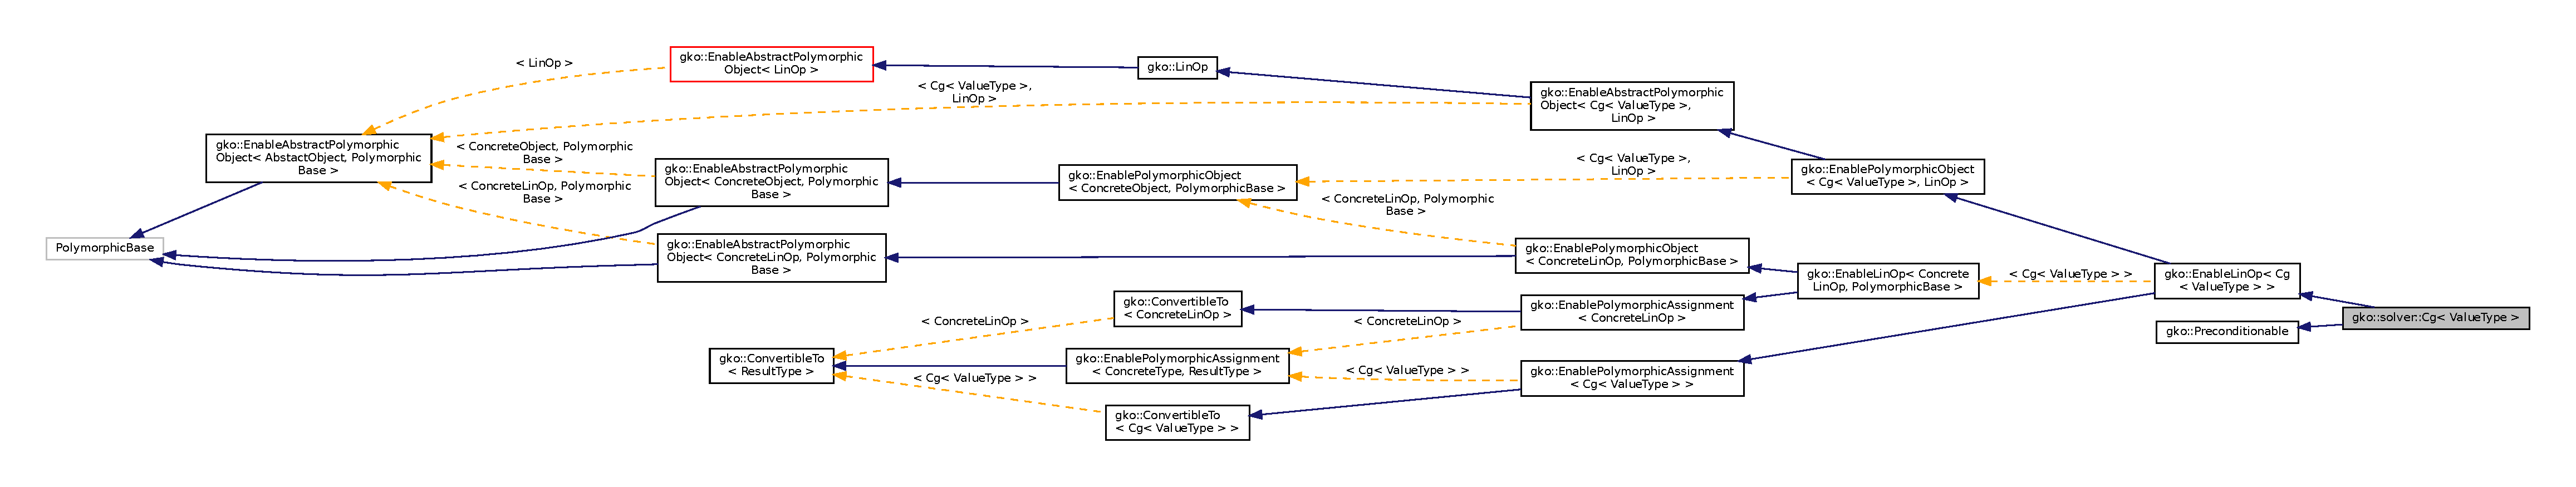
\includegraphics[width=350pt]{classgko_1_1solver_1_1Cg__coll__graph}
\end{center}
\end{figure}
\doxysubsection*{Classes}
\begin{DoxyCompactItemize}
\item 
class \mbox{\hyperlink{classgko_1_1solver_1_1Cg_1_1Factory}{Factory}}
\item 
struct \mbox{\hyperlink{structgko_1_1solver_1_1Cg_1_1parameters__type}{parameters\+\_\+type}}
\end{DoxyCompactItemize}
\doxysubsection*{Public Types}
\begin{DoxyCompactItemize}
\item 
\mbox{\Hypertarget{classgko_1_1solver_1_1Cg_a010f8f5b0b315108a3990052a73f80b0}\label{classgko_1_1solver_1_1Cg_a010f8f5b0b315108a3990052a73f80b0}} 
using {\bfseries value\+\_\+type} = Value\+Type
\end{DoxyCompactItemize}
\doxysubsection*{Public Member Functions}
\begin{DoxyCompactItemize}
\item 
std\+::shared\+\_\+ptr$<$ const \mbox{\hyperlink{classgko_1_1LinOp}{Lin\+Op}} $>$ \mbox{\hyperlink{classgko_1_1solver_1_1Cg_a09d50a99fdc668316757ee253386ad2a}{get\+\_\+system\+\_\+matrix}} () const
\begin{DoxyCompactList}\small\item\em Gets the system operator (matrix) of the linear system. \end{DoxyCompactList}\item 
\mbox{\Hypertarget{classgko_1_1solver_1_1Cg_a548b5ff27c59e50f78eb96a0463453ae}\label{classgko_1_1solver_1_1Cg_a548b5ff27c59e50f78eb96a0463453ae}} 
const \mbox{\hyperlink{structgko_1_1solver_1_1Cg_1_1parameters__type}{parameters\+\_\+type}} \& {\bfseries get\+\_\+parameters} () const
\end{DoxyCompactItemize}
\doxysubsection*{Static Public Member Functions}
\begin{DoxyCompactItemize}
\item 
\mbox{\Hypertarget{classgko_1_1solver_1_1Cg_a3d16ac7e3132362573b9af81cbccdf69}\label{classgko_1_1solver_1_1Cg_a3d16ac7e3132362573b9af81cbccdf69}} 
static auto {\bfseries build} () -\/$>$ decltype(\mbox{\hyperlink{classgko_1_1solver_1_1Cg_1_1Factory}{Factory}} \+::create())
\end{DoxyCompactItemize}
\doxysubsection*{Friends}
\begin{DoxyCompactItemize}
\item 
\mbox{\Hypertarget{classgko_1_1solver_1_1Cg_addd5cadb50dadd7e118776aeee9eb1c4}\label{classgko_1_1solver_1_1Cg_addd5cadb50dadd7e118776aeee9eb1c4}} 
class {\bfseries Enable\+Lin\+Op$<$ Cg $>$}
\item 
\mbox{\Hypertarget{classgko_1_1solver_1_1Cg_a4a8963db94d0c3f4136daf08823c6b09}\label{classgko_1_1solver_1_1Cg_a4a8963db94d0c3f4136daf08823c6b09}} 
class {\bfseries Enable\+Polymorphic\+Object$<$ Cg, Lin\+Op $>$}
\end{DoxyCompactItemize}


\doxysubsection{Detailed Description}
\subsubsection*{template$<$typename Value\+Type = default\+\_\+precision$>$\newline
class gko\+::solver\+::\+Cg$<$ Value\+Type $>$}

CG or the conjugate gradient method is an iterative type Krylov subspace method which is suitable for symmetric positive definite methods. 

Though this method performs very well for symmetric positive definite matrices, it is in general not suitable for general matrices.

The implementation in Ginkgo makes use of the merged kernel to make the best use of data locality. The inner operations in one iteration of CG are merged into 2 separate steps.


\begin{DoxyTemplParams}{Template Parameters}
{\em Value\+Type} & precision of matrix elements \\
\hline
\end{DoxyTemplParams}


\doxysubsection{Member Function Documentation}
\mbox{\Hypertarget{classgko_1_1solver_1_1Cg_a09d50a99fdc668316757ee253386ad2a}\label{classgko_1_1solver_1_1Cg_a09d50a99fdc668316757ee253386ad2a}} 
\index{gko::solver::Cg$<$ ValueType $>$@{gko::solver::Cg$<$ ValueType $>$}!get\_system\_matrix@{get\_system\_matrix}}
\index{get\_system\_matrix@{get\_system\_matrix}!gko::solver::Cg$<$ ValueType $>$@{gko::solver::Cg$<$ ValueType $>$}}
\doxysubsubsection{\texorpdfstring{get\_system\_matrix()}{get\_system\_matrix()}}
{\footnotesize\ttfamily template$<$typename Value\+Type  = default\+\_\+precision$>$ \\
std\+::shared\+\_\+ptr$<$const \mbox{\hyperlink{classgko_1_1LinOp}{Lin\+Op}}$>$ \mbox{\hyperlink{classgko_1_1solver_1_1Cg}{gko\+::solver\+::\+Cg}}$<$ Value\+Type $>$\+::get\+\_\+system\+\_\+matrix (\begin{DoxyParamCaption}{ }\end{DoxyParamCaption}) const\hspace{0.3cm}{\ttfamily [inline]}}



Gets the system operator (matrix) of the linear system. 

\begin{DoxyReturn}{Returns}
the system operator (matrix) 
\end{DoxyReturn}


The documentation for this class was generated from the following file\+:\begin{DoxyCompactItemize}
\item 
ginkgo/core/solver/cg.\+hpp (ccf35426a)\end{DoxyCompactItemize}

\hypertarget{classgko_1_1solver_1_1Cgs}{}\section{gko\+:\+:solver\+:\+:Cgs$<$ Value\+Type $>$ Class Template Reference}
\label{classgko_1_1solver_1_1Cgs}\index{gko\+::solver\+::\+Cgs$<$ Value\+Type $>$@{gko\+::solver\+::\+Cgs$<$ Value\+Type $>$}}


C\+GS or the conjugate gradient square method is an iterative type Krylov subspace method which is suitable for general systems.  




{\ttfamily \#include $<$ginkgo/core/solver/cgs.\+hpp$>$}



Collaboration diagram for gko\+:\+:solver\+:\+:Cgs$<$ Value\+Type $>$\+:
\nopagebreak
\begin{figure}[H]
\begin{center}
\leavevmode
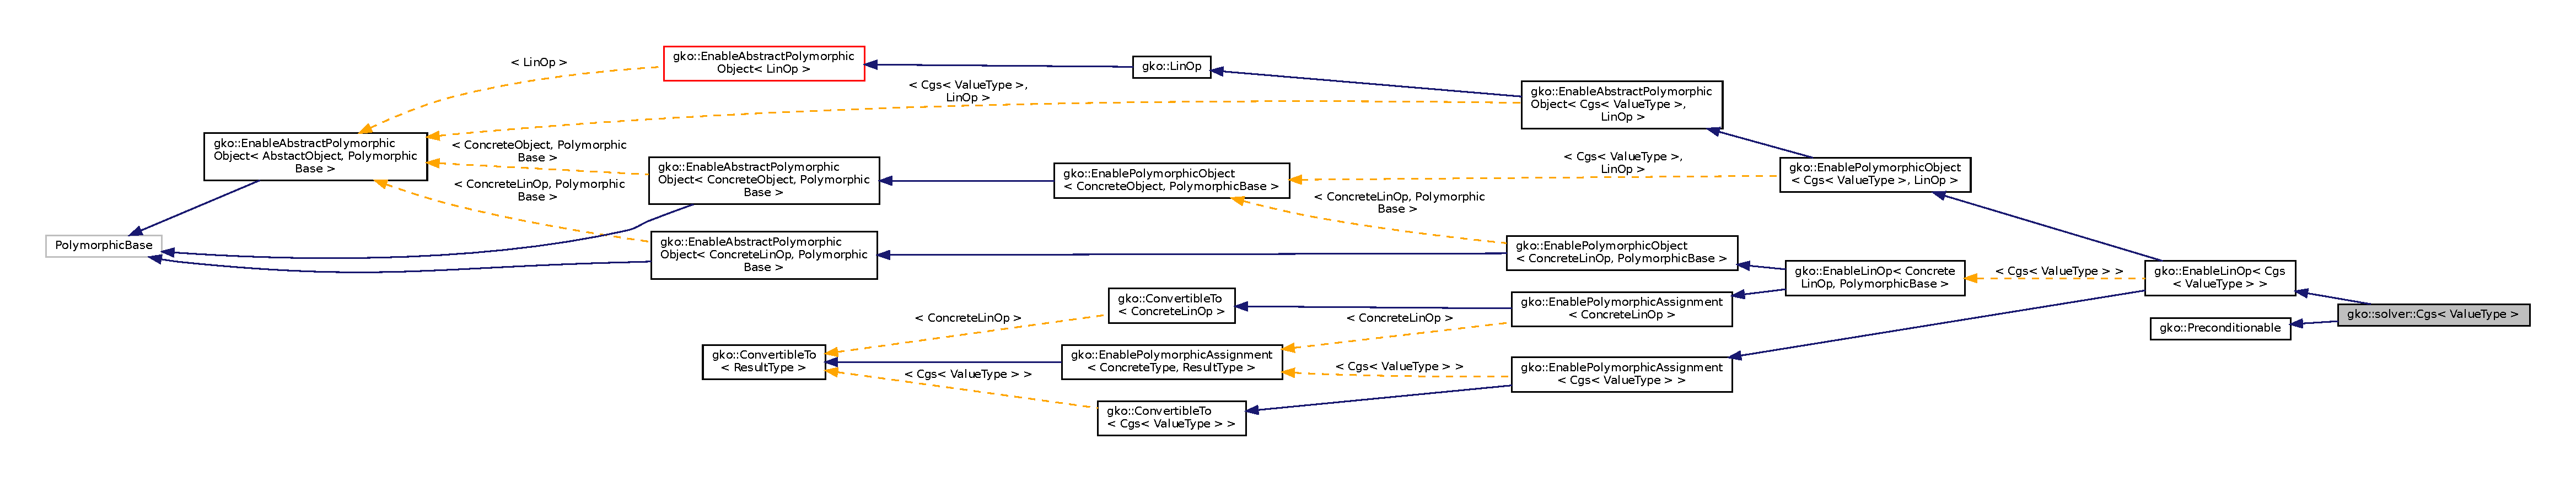
\includegraphics[width=350pt]{classgko_1_1solver_1_1Cgs__coll__graph}
\end{center}
\end{figure}
\subsection*{Classes}
\begin{DoxyCompactItemize}
\item 
class \hyperlink{classgko_1_1solver_1_1Cgs_1_1Factory}{Factory}
\item 
struct \hyperlink{structgko_1_1solver_1_1Cgs_1_1parameters__type}{parameters\+\_\+type}
\end{DoxyCompactItemize}
\subsection*{Public Types}
\begin{DoxyCompactItemize}
\item 
\mbox{\Hypertarget{classgko_1_1solver_1_1Cgs_a4dce78f8e1e2330a4dc576fa68ea10da}\label{classgko_1_1solver_1_1Cgs_a4dce78f8e1e2330a4dc576fa68ea10da}} 
using {\bfseries value\+\_\+type} = Value\+Type
\end{DoxyCompactItemize}
\subsection*{Public Member Functions}
\begin{DoxyCompactItemize}
\item 
std\+::shared\+\_\+ptr$<$ const \hyperlink{classgko_1_1LinOp}{Lin\+Op} $>$ \hyperlink{classgko_1_1solver_1_1Cgs_aa537b2e6b7ccf95e96b4100866da1770}{get\+\_\+system\+\_\+matrix} () const
\begin{DoxyCompactList}\small\item\em Gets the system operator (matrix) of the linear system. \end{DoxyCompactList}\item 
std\+::shared\+\_\+ptr$<$ const \hyperlink{classgko_1_1LinOp}{Lin\+Op} $>$ \hyperlink{classgko_1_1solver_1_1Cgs_ad349dc1381dfdcb7a47223908806dcc7}{get\+\_\+preconditioner} () const override
\begin{DoxyCompactList}\small\item\em Returns the preconditioner operator used by the solver. \end{DoxyCompactList}\item 
\mbox{\Hypertarget{classgko_1_1solver_1_1Cgs_a9ac2a7b0f0b14f3308be1988221c22d0}\label{classgko_1_1solver_1_1Cgs_a9ac2a7b0f0b14f3308be1988221c22d0}} 
const \hyperlink{structgko_1_1solver_1_1Cgs_1_1parameters__type}{parameters\+\_\+type} \& {\bfseries get\+\_\+parameters} () const
\end{DoxyCompactItemize}
\subsection*{Static Public Member Functions}
\begin{DoxyCompactItemize}
\item 
\mbox{\Hypertarget{classgko_1_1solver_1_1Cgs_ace0362ace1d2d1fd2e6322af973bca08}\label{classgko_1_1solver_1_1Cgs_ace0362ace1d2d1fd2e6322af973bca08}} 
static auto {\bfseries build} () -\/$>$ decltype(\hyperlink{classgko_1_1EnableDefaultFactory_a1d077101d9e788e6c65f088612d14cc3}{Factory\+::create}())
\end{DoxyCompactItemize}
\subsection*{Friends}
\begin{DoxyCompactItemize}
\item 
\mbox{\Hypertarget{classgko_1_1solver_1_1Cgs_abd9976d7b04021c8ba86dc8cd3c7c21b}\label{classgko_1_1solver_1_1Cgs_abd9976d7b04021c8ba86dc8cd3c7c21b}} 
class {\bfseries Enable\+Lin\+Op$<$ Cgs $>$}
\item 
\mbox{\Hypertarget{classgko_1_1solver_1_1Cgs_af58c1f415ba0ca2591898b3913acd0d2}\label{classgko_1_1solver_1_1Cgs_af58c1f415ba0ca2591898b3913acd0d2}} 
class {\bfseries Enable\+Polymorphic\+Object$<$ Cgs, Lin\+Op $>$}
\end{DoxyCompactItemize}


\subsection{Detailed Description}
\subsubsection*{template$<$typename Value\+Type = default\+\_\+precision$>$\newline
class gko\+::solver\+::\+Cgs$<$ Value\+Type $>$}

C\+GS or the conjugate gradient square method is an iterative type Krylov subspace method which is suitable for general systems. 

The implementation in Ginkgo makes use of the merged kernel to make the best use of data locality. The inner operations in one iteration of C\+GS are merged into 3 separate steps.


\begin{DoxyTemplParams}{Template Parameters}
{\em Value\+Type} & precision of matrix elements \\
\hline
\end{DoxyTemplParams}


\subsection{Member Function Documentation}
\mbox{\Hypertarget{classgko_1_1solver_1_1Cgs_ad349dc1381dfdcb7a47223908806dcc7}\label{classgko_1_1solver_1_1Cgs_ad349dc1381dfdcb7a47223908806dcc7}} 
\index{gko\+::solver\+::\+Cgs@{gko\+::solver\+::\+Cgs}!get\+\_\+preconditioner@{get\+\_\+preconditioner}}
\index{get\+\_\+preconditioner@{get\+\_\+preconditioner}!gko\+::solver\+::\+Cgs@{gko\+::solver\+::\+Cgs}}
\subsubsection{\texorpdfstring{get\+\_\+preconditioner()}{get\_preconditioner()}}
{\footnotesize\ttfamily template$<$typename Value\+Type  = default\+\_\+precision$>$ \\
std\+::shared\+\_\+ptr$<$const \hyperlink{classgko_1_1LinOp}{Lin\+Op}$>$ \hyperlink{classgko_1_1solver_1_1Cgs}{gko\+::solver\+::\+Cgs}$<$ Value\+Type $>$\+::get\+\_\+preconditioner (\begin{DoxyParamCaption}{ }\end{DoxyParamCaption}) const\hspace{0.3cm}{\ttfamily [override]}, {\ttfamily [virtual]}}



Returns the preconditioner operator used by the solver. 

\begin{DoxyReturn}{Returns}
the preconditioner operator used by the solver 
\end{DoxyReturn}


Implements \hyperlink{classgko_1_1Preconditionable_ad9545089aef0dfc83bc7a74e5bf1d748}{gko\+::\+Preconditionable}.

\mbox{\Hypertarget{classgko_1_1solver_1_1Cgs_aa537b2e6b7ccf95e96b4100866da1770}\label{classgko_1_1solver_1_1Cgs_aa537b2e6b7ccf95e96b4100866da1770}} 
\index{gko\+::solver\+::\+Cgs@{gko\+::solver\+::\+Cgs}!get\+\_\+system\+\_\+matrix@{get\+\_\+system\+\_\+matrix}}
\index{get\+\_\+system\+\_\+matrix@{get\+\_\+system\+\_\+matrix}!gko\+::solver\+::\+Cgs@{gko\+::solver\+::\+Cgs}}
\subsubsection{\texorpdfstring{get\+\_\+system\+\_\+matrix()}{get\_system\_matrix()}}
{\footnotesize\ttfamily template$<$typename Value\+Type  = default\+\_\+precision$>$ \\
std\+::shared\+\_\+ptr$<$const \hyperlink{classgko_1_1LinOp}{Lin\+Op}$>$ \hyperlink{classgko_1_1solver_1_1Cgs}{gko\+::solver\+::\+Cgs}$<$ Value\+Type $>$\+::get\+\_\+system\+\_\+matrix (\begin{DoxyParamCaption}{ }\end{DoxyParamCaption}) const}



Gets the system operator (matrix) of the linear system. 

\begin{DoxyReturn}{Returns}
the system operator (matrix) 
\end{DoxyReturn}


The documentation for this class was generated from the following file\+:\begin{DoxyCompactItemize}
\item 
ginkgo/core/solver/cgs.\+hpp (99beb325)\end{DoxyCompactItemize}

\hypertarget{classgko_1_1matrix_1_1Csr_1_1classical}{}\doxysection{gko\+::matrix\+::Csr$<$ Value\+Type, Index\+Type $>$\+::classical Class Reference}
\label{classgko_1_1matrix_1_1Csr_1_1classical}\index{gko::matrix::Csr$<$ ValueType, IndexType $>$::classical@{gko::matrix::Csr$<$ ValueType, IndexType $>$::classical}}


classical is a \mbox{\hyperlink{classgko_1_1matrix_1_1Csr_1_1strategy__type}{strategy\+\_\+type}} which uses the same number of threads on each row.  




{\ttfamily \#include $<$ginkgo/core/matrix/csr.\+hpp$>$}



Collaboration diagram for gko\+::matrix\+::Csr$<$ Value\+Type, Index\+Type $>$\+::classical\+:
\nopagebreak
\begin{figure}[H]
\begin{center}
\leavevmode
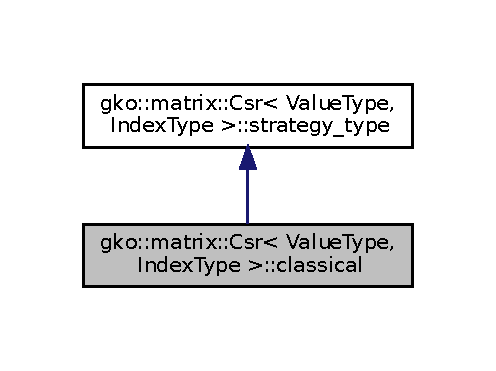
\includegraphics[width=238pt]{classgko_1_1matrix_1_1Csr_1_1classical__coll__graph}
\end{center}
\end{figure}
\doxysubsection*{Public Member Functions}
\begin{DoxyCompactItemize}
\item 
\mbox{\Hypertarget{classgko_1_1matrix_1_1Csr_1_1classical_a98620198be4dc96d661b7bd1007407b2}\label{classgko_1_1matrix_1_1Csr_1_1classical_a98620198be4dc96d661b7bd1007407b2}} 
\mbox{\hyperlink{classgko_1_1matrix_1_1Csr_1_1classical_a98620198be4dc96d661b7bd1007407b2}{classical}} ()
\begin{DoxyCompactList}\small\item\em Creates a classical strategy. \end{DoxyCompactList}\item 
void \mbox{\hyperlink{classgko_1_1matrix_1_1Csr_1_1classical_a2844a228c3a3f827c8ad9cab5c0e453f}{process}} (const \mbox{\hyperlink{classgko_1_1Array}{Array}}$<$ index\+\_\+type $>$ \&mtx\+\_\+row\+\_\+ptrs, \mbox{\hyperlink{classgko_1_1Array}{Array}}$<$ index\+\_\+type $>$ $\ast$mtx\+\_\+srow) override
\begin{DoxyCompactList}\small\item\em Computes srow according to row pointers. \end{DoxyCompactList}\item 
int64\+\_\+t \mbox{\hyperlink{classgko_1_1matrix_1_1Csr_1_1classical_ae99f47abc647f84793d9f84a9605a77d}{clac\+\_\+size}} (const int64\+\_\+t nnz) override
\begin{DoxyCompactList}\small\item\em Computes the srow size according to the number of nonzeros. \end{DoxyCompactList}\item 
\mbox{\Hypertarget{classgko_1_1matrix_1_1Csr_1_1classical_afe21530a9de0bdd806068081cda597b3}\label{classgko_1_1matrix_1_1Csr_1_1classical_afe21530a9de0bdd806068081cda597b3}} 
index\+\_\+type {\bfseries get\+\_\+max\+\_\+length\+\_\+per\+\_\+row} () const noexcept
\end{DoxyCompactItemize}


\doxysubsection{Detailed Description}
\subsubsection*{template$<$typename Value\+Type = default\+\_\+precision, typename Index\+Type = int32$>$\newline
class gko\+::matrix\+::\+Csr$<$ Value\+Type, Index\+Type $>$\+::classical}

classical is a \mbox{\hyperlink{classgko_1_1matrix_1_1Csr_1_1strategy__type}{strategy\+\_\+type}} which uses the same number of threads on each row. 

Classical strategy uses multithreads to calculate on parts of rows and then do a reduction of these threads results. The number of threads per row depends on the max number of stored elements per row. 

\doxysubsection{Member Function Documentation}
\mbox{\Hypertarget{classgko_1_1matrix_1_1Csr_1_1classical_ae99f47abc647f84793d9f84a9605a77d}\label{classgko_1_1matrix_1_1Csr_1_1classical_ae99f47abc647f84793d9f84a9605a77d}} 
\index{gko::matrix::Csr$<$ ValueType, IndexType $>$::classical@{gko::matrix::Csr$<$ ValueType, IndexType $>$::classical}!clac\_size@{clac\_size}}
\index{clac\_size@{clac\_size}!gko::matrix::Csr$<$ ValueType, IndexType $>$::classical@{gko::matrix::Csr$<$ ValueType, IndexType $>$::classical}}
\doxysubsubsection{\texorpdfstring{clac\_size()}{clac\_size()}}
{\footnotesize\ttfamily template$<$typename Value\+Type = default\+\_\+precision, typename Index\+Type = int32$>$ \\
int64\+\_\+t \mbox{\hyperlink{classgko_1_1matrix_1_1Csr}{gko\+::matrix\+::\+Csr}}$<$ Value\+Type, Index\+Type $>$\+::classical\+::clac\+\_\+size (\begin{DoxyParamCaption}\item[{const int64\+\_\+t}]{nnz }\end{DoxyParamCaption})\hspace{0.3cm}{\ttfamily [inline]}, {\ttfamily [override]}, {\ttfamily [virtual]}}



Computes the srow size according to the number of nonzeros. 


\begin{DoxyParams}{Parameters}
{\em nnz} & the number of nonzeros\\
\hline
\end{DoxyParams}
\begin{DoxyReturn}{Returns}
the size of srow 
\end{DoxyReturn}


Implements \mbox{\hyperlink{classgko_1_1matrix_1_1Csr_1_1strategy__type_a07a6dda9dd04ed8abd914f3a69f330f2}{gko\+::matrix\+::\+Csr$<$ Value\+Type, Index\+Type $>$\+::strategy\+\_\+type}}.

\mbox{\Hypertarget{classgko_1_1matrix_1_1Csr_1_1classical_a2844a228c3a3f827c8ad9cab5c0e453f}\label{classgko_1_1matrix_1_1Csr_1_1classical_a2844a228c3a3f827c8ad9cab5c0e453f}} 
\index{gko::matrix::Csr$<$ ValueType, IndexType $>$::classical@{gko::matrix::Csr$<$ ValueType, IndexType $>$::classical}!process@{process}}
\index{process@{process}!gko::matrix::Csr$<$ ValueType, IndexType $>$::classical@{gko::matrix::Csr$<$ ValueType, IndexType $>$::classical}}
\doxysubsubsection{\texorpdfstring{process()}{process()}}
{\footnotesize\ttfamily template$<$typename Value\+Type = default\+\_\+precision, typename Index\+Type = int32$>$ \\
void \mbox{\hyperlink{classgko_1_1matrix_1_1Csr}{gko\+::matrix\+::\+Csr}}$<$ Value\+Type, Index\+Type $>$\+::classical\+::process (\begin{DoxyParamCaption}\item[{const \mbox{\hyperlink{classgko_1_1Array}{Array}}$<$ index\+\_\+type $>$ \&}]{mtx\+\_\+row\+\_\+ptrs,  }\item[{\mbox{\hyperlink{classgko_1_1Array}{Array}}$<$ index\+\_\+type $>$ $\ast$}]{mtx\+\_\+srow }\end{DoxyParamCaption})\hspace{0.3cm}{\ttfamily [inline]}, {\ttfamily [override]}, {\ttfamily [virtual]}}



Computes srow according to row pointers. 


\begin{DoxyParams}{Parameters}
{\em mtx\+\_\+row\+\_\+ptrs} & the row pointers of the matrix \\
\hline
{\em mtx\+\_\+srow} & the srow of the matrix \\
\hline
\end{DoxyParams}


Implements \mbox{\hyperlink{classgko_1_1matrix_1_1Csr_1_1strategy__type_a58bda9208766e57d861262d4059b65b4}{gko\+::matrix\+::\+Csr$<$ Value\+Type, Index\+Type $>$\+::strategy\+\_\+type}}.



References gko\+::\+Array$<$ Value\+Type $>$\+::get\+\_\+const\+\_\+data(), gko\+::\+Array$<$ Value\+Type $>$\+::get\+\_\+executor(), and gko\+::\+Array$<$ Value\+Type $>$\+::get\+\_\+num\+\_\+elems().



Referenced by gko\+::matrix\+::\+Csr$<$ Value\+Type, Index\+Type $>$\+::automatical\+::process().



The documentation for this class was generated from the following file\+:\begin{DoxyCompactItemize}
\item 
ginkgo/core/matrix/csr.\+hpp (196fd04da)\end{DoxyCompactItemize}

\hypertarget{classgko_1_1matrix_1_1Hybrid_1_1column__limit}{}\doxysection{gko\+::matrix\+::Hybrid$<$ Value\+Type, Index\+Type $>$\+::column\+\_\+limit Class Reference}
\label{classgko_1_1matrix_1_1Hybrid_1_1column__limit}\index{gko::matrix::Hybrid$<$ ValueType, IndexType $>$::column\_limit@{gko::matrix::Hybrid$<$ ValueType, IndexType $>$::column\_limit}}


\mbox{\hyperlink{classgko_1_1matrix_1_1Hybrid_1_1column__limit}{column\+\_\+limit}} is a \mbox{\hyperlink{classgko_1_1matrix_1_1Hybrid_1_1strategy__type}{strategy\+\_\+type}} which decides the number of stored elements per row of the ell part by specifying the number of columns.  




{\ttfamily \#include $<$ginkgo/core/matrix/hybrid.\+hpp$>$}



Collaboration diagram for gko\+::matrix\+::Hybrid$<$ Value\+Type, Index\+Type $>$\+::column\+\_\+limit\+:
\nopagebreak
\begin{figure}[H]
\begin{center}
\leavevmode
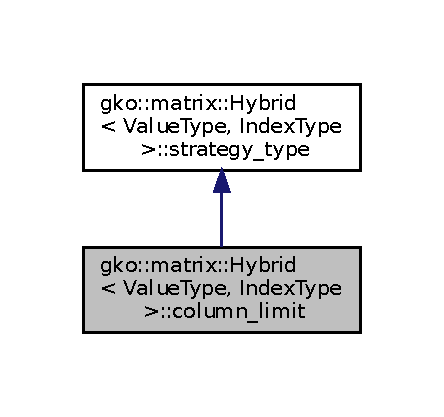
\includegraphics[width=213pt]{classgko_1_1matrix_1_1Hybrid_1_1column__limit__coll__graph}
\end{center}
\end{figure}
\doxysubsection*{Public Member Functions}
\begin{DoxyCompactItemize}
\item 
\mbox{\hyperlink{classgko_1_1matrix_1_1Hybrid_1_1column__limit_ac686f3f99034bffd091bd934bd1cf9f9}{column\+\_\+limit}} (\mbox{\hyperlink{namespacegko_a6e5c95df0ae4e47aab2f604a22d98ee7}{size\+\_\+type}} num\+\_\+column=0)
\begin{DoxyCompactList}\small\item\em Creates a \mbox{\hyperlink{classgko_1_1matrix_1_1Hybrid_1_1column__limit}{column\+\_\+limit}} strategy. \end{DoxyCompactList}\item 
\mbox{\hyperlink{namespacegko_a6e5c95df0ae4e47aab2f604a22d98ee7}{size\+\_\+type}} \mbox{\hyperlink{classgko_1_1matrix_1_1Hybrid_1_1column__limit_afb410def66106b711ac094fd31d48aba}{compute\+\_\+ell\+\_\+num\+\_\+stored\+\_\+elements\+\_\+per\+\_\+row}} (\mbox{\hyperlink{classgko_1_1Array}{Array}}$<$ \mbox{\hyperlink{namespacegko_a6e5c95df0ae4e47aab2f604a22d98ee7}{size\+\_\+type}} $>$ $\ast$row\+\_\+nnz) const override
\begin{DoxyCompactList}\small\item\em Computes the number of stored elements per row of the ell part. \end{DoxyCompactList}\end{DoxyCompactItemize}


\doxysubsection{Detailed Description}
\subsubsection*{template$<$typename Value\+Type = default\+\_\+precision, typename Index\+Type = int32$>$\newline
class gko\+::matrix\+::\+Hybrid$<$ Value\+Type, Index\+Type $>$\+::column\+\_\+limit}

\mbox{\hyperlink{classgko_1_1matrix_1_1Hybrid_1_1column__limit}{column\+\_\+limit}} is a \mbox{\hyperlink{classgko_1_1matrix_1_1Hybrid_1_1strategy__type}{strategy\+\_\+type}} which decides the number of stored elements per row of the ell part by specifying the number of columns. 

\doxysubsection{Constructor \& Destructor Documentation}
\mbox{\Hypertarget{classgko_1_1matrix_1_1Hybrid_1_1column__limit_ac686f3f99034bffd091bd934bd1cf9f9}\label{classgko_1_1matrix_1_1Hybrid_1_1column__limit_ac686f3f99034bffd091bd934bd1cf9f9}} 
\index{gko::matrix::Hybrid$<$ ValueType, IndexType $>$::column\_limit@{gko::matrix::Hybrid$<$ ValueType, IndexType $>$::column\_limit}!column\_limit@{column\_limit}}
\index{column\_limit@{column\_limit}!gko::matrix::Hybrid$<$ ValueType, IndexType $>$::column\_limit@{gko::matrix::Hybrid$<$ ValueType, IndexType $>$::column\_limit}}
\doxysubsubsection{\texorpdfstring{column\_limit()}{column\_limit()}}
{\footnotesize\ttfamily template$<$typename Value\+Type = default\+\_\+precision, typename Index\+Type = int32$>$ \\
\mbox{\hyperlink{classgko_1_1matrix_1_1Hybrid}{gko\+::matrix\+::\+Hybrid}}$<$ Value\+Type, Index\+Type $>$\+::column\+\_\+limit\+::column\+\_\+limit (\begin{DoxyParamCaption}\item[{\mbox{\hyperlink{namespacegko_a6e5c95df0ae4e47aab2f604a22d98ee7}{size\+\_\+type}}}]{num\+\_\+column = {\ttfamily 0} }\end{DoxyParamCaption})\hspace{0.3cm}{\ttfamily [inline]}, {\ttfamily [explicit]}}



Creates a \mbox{\hyperlink{classgko_1_1matrix_1_1Hybrid_1_1column__limit}{column\+\_\+limit}} strategy. 


\begin{DoxyParams}{Parameters}
{\em num\+\_\+column} & the specified number of columns of the ell part \\
\hline
\end{DoxyParams}


\doxysubsection{Member Function Documentation}
\mbox{\Hypertarget{classgko_1_1matrix_1_1Hybrid_1_1column__limit_afb410def66106b711ac094fd31d48aba}\label{classgko_1_1matrix_1_1Hybrid_1_1column__limit_afb410def66106b711ac094fd31d48aba}} 
\index{gko::matrix::Hybrid$<$ ValueType, IndexType $>$::column\_limit@{gko::matrix::Hybrid$<$ ValueType, IndexType $>$::column\_limit}!compute\_ell\_num\_stored\_elements\_per\_row@{compute\_ell\_num\_stored\_elements\_per\_row}}
\index{compute\_ell\_num\_stored\_elements\_per\_row@{compute\_ell\_num\_stored\_elements\_per\_row}!gko::matrix::Hybrid$<$ ValueType, IndexType $>$::column\_limit@{gko::matrix::Hybrid$<$ ValueType, IndexType $>$::column\_limit}}
\doxysubsubsection{\texorpdfstring{compute\_ell\_num\_stored\_elements\_per\_row()}{compute\_ell\_num\_stored\_elements\_per\_row()}}
{\footnotesize\ttfamily template$<$typename Value\+Type = default\+\_\+precision, typename Index\+Type = int32$>$ \\
\mbox{\hyperlink{namespacegko_a6e5c95df0ae4e47aab2f604a22d98ee7}{size\+\_\+type}} \mbox{\hyperlink{classgko_1_1matrix_1_1Hybrid}{gko\+::matrix\+::\+Hybrid}}$<$ Value\+Type, Index\+Type $>$\+::column\+\_\+limit\+::compute\+\_\+ell\+\_\+num\+\_\+stored\+\_\+elements\+\_\+per\+\_\+row (\begin{DoxyParamCaption}\item[{\mbox{\hyperlink{classgko_1_1Array}{Array}}$<$ \mbox{\hyperlink{namespacegko_a6e5c95df0ae4e47aab2f604a22d98ee7}{size\+\_\+type}} $>$ $\ast$}]{row\+\_\+nnz }\end{DoxyParamCaption}) const\hspace{0.3cm}{\ttfamily [inline]}, {\ttfamily [override]}, {\ttfamily [virtual]}}



Computes the number of stored elements per row of the ell part. 


\begin{DoxyParams}{Parameters}
{\em row\+\_\+nnz} & the number of nonzeros of each row\\
\hline
\end{DoxyParams}
\begin{DoxyReturn}{Returns}
the number of stored elements per row of the ell part 
\end{DoxyReturn}


Implements \mbox{\hyperlink{classgko_1_1matrix_1_1Hybrid_1_1strategy__type_a0a0cd4024f27c7d0f286f35fc0a6de60}{gko\+::matrix\+::\+Hybrid$<$ Value\+Type, Index\+Type $>$\+::strategy\+\_\+type}}.



The documentation for this class was generated from the following file\+:\begin{DoxyCompactItemize}
\item 
ginkgo/core/matrix/hybrid.\+hpp (4b82e692f)\end{DoxyCompactItemize}

\hypertarget{classgko_1_1Combination}{}\section{gko\+:\+:Combination$<$ Value\+Type $>$ Class Template Reference}
\label{classgko_1_1Combination}\index{gko\+::\+Combination$<$ Value\+Type $>$@{gko\+::\+Combination$<$ Value\+Type $>$}}


The \hyperlink{classgko_1_1Combination}{Combination} class can be used to construct a linear combination of multiple linear operators `c1 $\ast$ op1 + c2 $\ast$ op2 + ...  




{\ttfamily \#include $<$ginkgo/core/base/combination.\+hpp$>$}



Collaboration diagram for gko\+:\+:Combination$<$ Value\+Type $>$\+:
\nopagebreak
\begin{figure}[H]
\begin{center}
\leavevmode
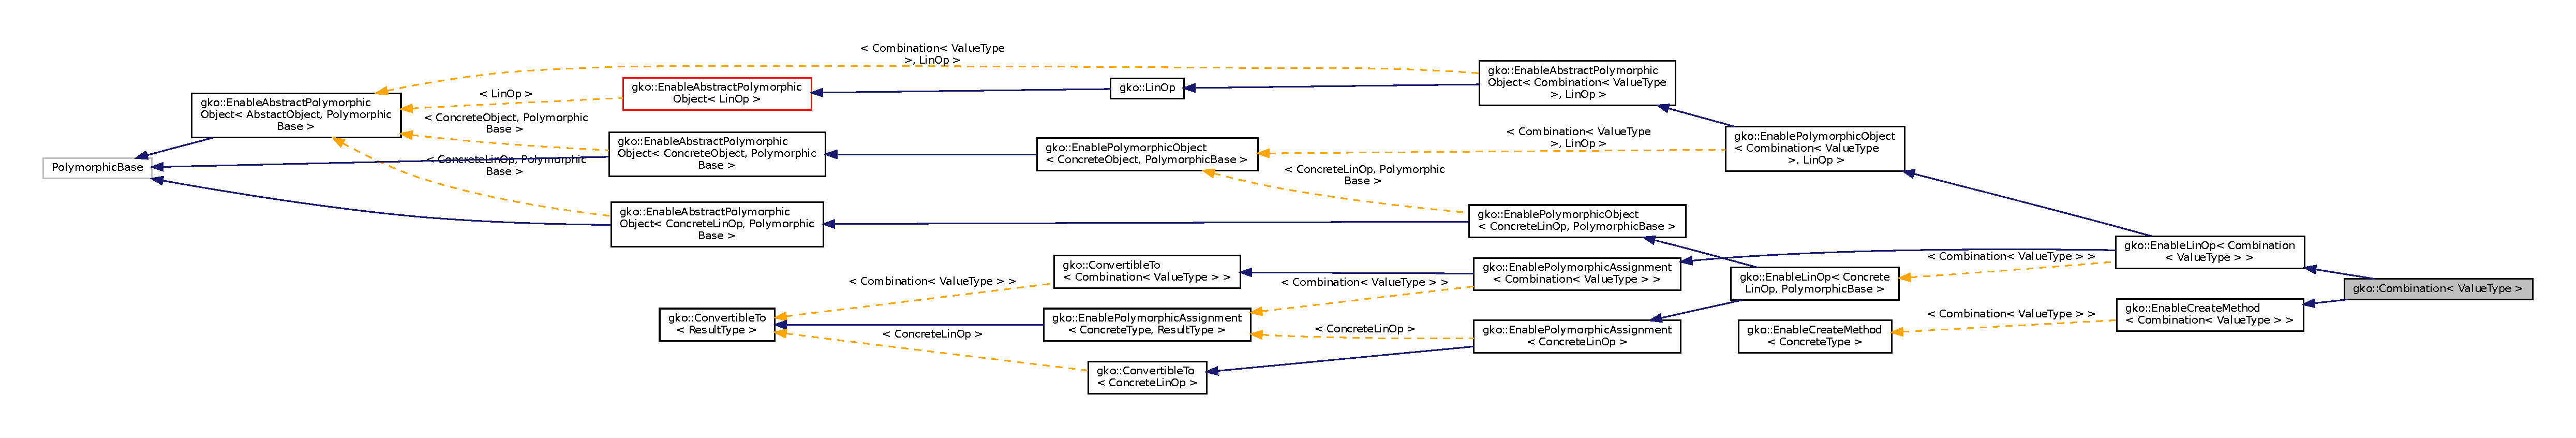
\includegraphics[width=350pt]{classgko_1_1Combination__coll__graph}
\end{center}
\end{figure}
\subsection*{Public Types}
\begin{DoxyCompactItemize}
\item 
\mbox{\Hypertarget{classgko_1_1Combination_a503b5d7f5f35f6ff697e44a850f10f9f}\label{classgko_1_1Combination_a503b5d7f5f35f6ff697e44a850f10f9f}} 
using {\bfseries value\+\_\+type} = Value\+Type
\end{DoxyCompactItemize}
\subsection*{Public Member Functions}
\begin{DoxyCompactItemize}
\item 
const std\+::vector$<$ std\+::shared\+\_\+ptr$<$ const \hyperlink{classgko_1_1LinOp}{Lin\+Op} $>$ $>$ \& \hyperlink{classgko_1_1Combination_ad5844423c39d70ee90d5dc432c83261f}{get\+\_\+coefficients} () const noexcept
\begin{DoxyCompactList}\small\item\em Returns a list of coefficients of the combination. \end{DoxyCompactList}\item 
const std\+::vector$<$ std\+::shared\+\_\+ptr$<$ const \hyperlink{classgko_1_1LinOp}{Lin\+Op} $>$ $>$ \& \hyperlink{classgko_1_1Combination_a75a81c2b91441ddea98949ef54f62441}{get\+\_\+operators} () const noexcept
\begin{DoxyCompactList}\small\item\em Returns a list of operators of the combination. \end{DoxyCompactList}\end{DoxyCompactItemize}
\subsection*{Friends}
\begin{DoxyCompactItemize}
\item 
\mbox{\Hypertarget{classgko_1_1Combination_ae096eca62ea7e5640d99ece073cf1194}\label{classgko_1_1Combination_ae096eca62ea7e5640d99ece073cf1194}} 
class {\bfseries Enable\+Polymorphic\+Object$<$ Combination, Lin\+Op $>$}
\item 
\mbox{\Hypertarget{classgko_1_1Combination_a54ec531b3585ab2f8572e20e3bebb9d1}\label{classgko_1_1Combination_a54ec531b3585ab2f8572e20e3bebb9d1}} 
class {\bfseries Enable\+Create\+Method$<$ Combination $>$}
\end{DoxyCompactItemize}
\subsection*{Additional Inherited Members}


\subsection{Detailed Description}
\subsubsection*{template$<$typename Value\+Type = default\+\_\+precision$>$\newline
class gko\+::\+Combination$<$ Value\+Type $>$}

The \hyperlink{classgko_1_1Combination}{Combination} class can be used to construct a linear combination of multiple linear operators `c1 $\ast$ op1 + c2 $\ast$ op2 + ... 


\begin{DoxyItemize}
\item ck $\ast$ opk`.
\end{DoxyItemize}


\begin{DoxyTemplParams}{Template Parameters}
{\em Value\+Type} & precision of input and result vectors \\
\hline
\end{DoxyTemplParams}


\subsection{Member Function Documentation}
\mbox{\Hypertarget{classgko_1_1Combination_ad5844423c39d70ee90d5dc432c83261f}\label{classgko_1_1Combination_ad5844423c39d70ee90d5dc432c83261f}} 
\index{gko\+::\+Combination@{gko\+::\+Combination}!get\+\_\+coefficients@{get\+\_\+coefficients}}
\index{get\+\_\+coefficients@{get\+\_\+coefficients}!gko\+::\+Combination@{gko\+::\+Combination}}
\subsubsection{\texorpdfstring{get\+\_\+coefficients()}{get\_coefficients()}}
{\footnotesize\ttfamily template$<$typename Value\+Type  = default\+\_\+precision$>$ \\
const std\+::vector$<$std\+::shared\+\_\+ptr$<$const \hyperlink{classgko_1_1LinOp}{Lin\+Op}$>$ $>$\& \hyperlink{classgko_1_1Combination}{gko\+::\+Combination}$<$ Value\+Type $>$\+::get\+\_\+coefficients (\begin{DoxyParamCaption}{ }\end{DoxyParamCaption}) const\hspace{0.3cm}{\ttfamily [noexcept]}}



Returns a list of coefficients of the combination. 

\begin{DoxyReturn}{Returns}
a list of coefficients 
\end{DoxyReturn}
\mbox{\Hypertarget{classgko_1_1Combination_a75a81c2b91441ddea98949ef54f62441}\label{classgko_1_1Combination_a75a81c2b91441ddea98949ef54f62441}} 
\index{gko\+::\+Combination@{gko\+::\+Combination}!get\+\_\+operators@{get\+\_\+operators}}
\index{get\+\_\+operators@{get\+\_\+operators}!gko\+::\+Combination@{gko\+::\+Combination}}
\subsubsection{\texorpdfstring{get\+\_\+operators()}{get\_operators()}}
{\footnotesize\ttfamily template$<$typename Value\+Type  = default\+\_\+precision$>$ \\
const std\+::vector$<$std\+::shared\+\_\+ptr$<$const \hyperlink{classgko_1_1LinOp}{Lin\+Op}$>$ $>$\& \hyperlink{classgko_1_1Combination}{gko\+::\+Combination}$<$ Value\+Type $>$\+::get\+\_\+operators (\begin{DoxyParamCaption}{ }\end{DoxyParamCaption}) const\hspace{0.3cm}{\ttfamily [noexcept]}}



Returns a list of operators of the combination. 

\begin{DoxyReturn}{Returns}
a list of operators 
\end{DoxyReturn}


References gko\+::\+Lin\+Op\+::get\+\_\+size(), gko\+::one(), and gko\+::zero().



The documentation for this class was generated from the following file\+:\begin{DoxyCompactItemize}
\item 
ginkgo/core/base/combination.\+hpp (99beb325)\end{DoxyCompactItemize}

\hypertarget{classgko_1_1stop_1_1Combined}{}\section{gko\+:\+:stop\+:\+:Combined Class Reference}
\label{classgko_1_1stop_1_1Combined}\index{gko\+::stop\+::\+Combined@{gko\+::stop\+::\+Combined}}


The \hyperlink{classgko_1_1stop_1_1Combined}{Combined} class is used to combine multiple criterions together through an OR operation.  




{\ttfamily \#include $<$ginkgo/core/stop/combined.\+hpp$>$}



Collaboration diagram for gko\+:\+:stop\+:\+:Combined\+:
\nopagebreak
\begin{figure}[H]
\begin{center}
\leavevmode
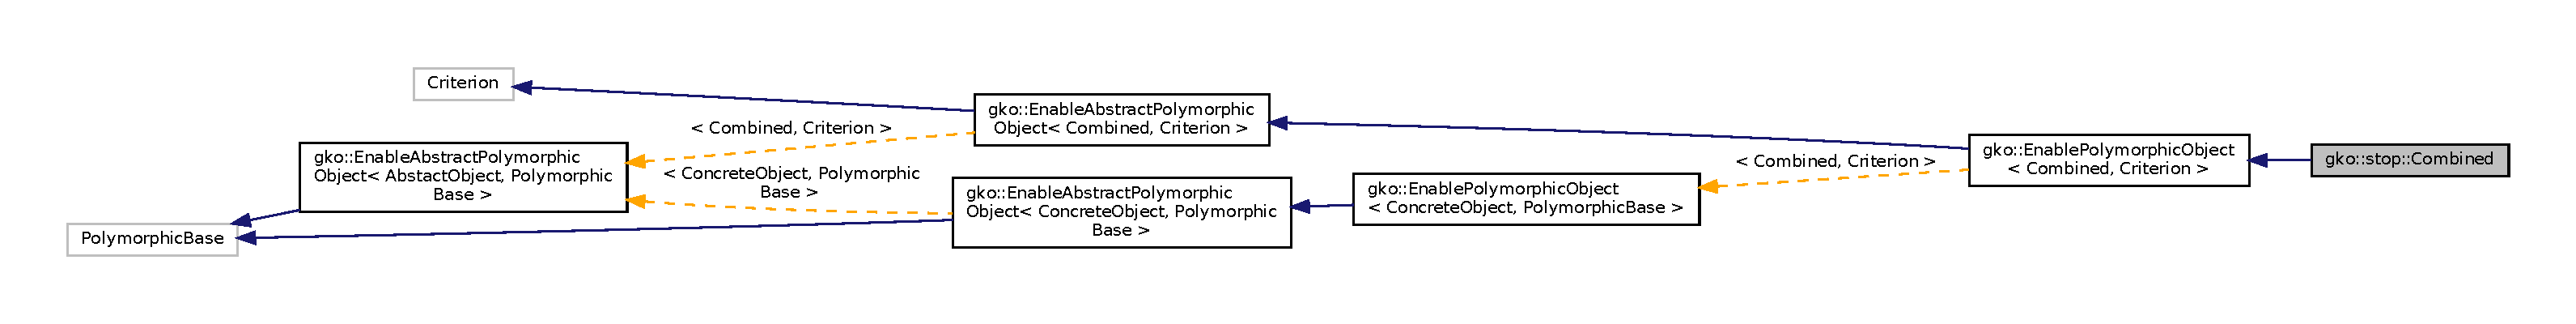
\includegraphics[width=350pt]{classgko_1_1stop_1_1Combined__coll__graph}
\end{center}
\end{figure}
\subsection*{Classes}
\begin{DoxyCompactItemize}
\item 
class \hyperlink{classgko_1_1stop_1_1Combined_1_1Factory}{Factory}
\item 
struct \hyperlink{structgko_1_1stop_1_1Combined_1_1parameters__type}{parameters\+\_\+type}
\end{DoxyCompactItemize}
\subsection*{Public Member Functions}
\begin{DoxyCompactItemize}
\item 
\mbox{\Hypertarget{classgko_1_1stop_1_1Combined_a0acc22e2dcbbf1493f9acb2fc77dbecd}\label{classgko_1_1stop_1_1Combined_a0acc22e2dcbbf1493f9acb2fc77dbecd}} 
const \hyperlink{structgko_1_1stop_1_1Combined_1_1parameters__type}{parameters\+\_\+type} \& {\bfseries get\+\_\+parameters} () const
\end{DoxyCompactItemize}
\subsection*{Static Public Member Functions}
\begin{DoxyCompactItemize}
\item 
\mbox{\Hypertarget{classgko_1_1stop_1_1Combined_a690e4d16114fc725080cdc8826c4ddc0}\label{classgko_1_1stop_1_1Combined_a690e4d16114fc725080cdc8826c4ddc0}} 
static auto {\bfseries build} () -\/$>$ decltype(\hyperlink{classgko_1_1EnableDefaultFactory_a1d077101d9e788e6c65f088612d14cc3}{Factory\+::create}())
\end{DoxyCompactItemize}
\subsection*{Friends}
\begin{DoxyCompactItemize}
\item 
\mbox{\Hypertarget{classgko_1_1stop_1_1Combined_a7c6977e97337814148e9c8ba5801ebf9}\label{classgko_1_1stop_1_1Combined_a7c6977e97337814148e9c8ba5801ebf9}} 
class {\bfseries Enable\+Polymorphic\+Object$<$ Combined, Criterion $>$}
\end{DoxyCompactItemize}


\subsection{Detailed Description}
The \hyperlink{classgko_1_1stop_1_1Combined}{Combined} class is used to combine multiple criterions together through an OR operation. 

The typical use case is to stop the iteration process if any of the criteria is fulfilled, e.\+g. a number of iterations, the relative residual norm has reached a threshold, etc. 

The documentation for this class was generated from the following file\+:\begin{DoxyCompactItemize}
\item 
ginkgo/core/stop/combined.\+hpp (edbc7156)\end{DoxyCompactItemize}

\hypertarget{classgko_1_1Composition}{}\section{gko\+:\+:Composition$<$ Value\+Type $>$ Class Template Reference}
\label{classgko_1_1Composition}\index{gko\+::\+Composition$<$ Value\+Type $>$@{gko\+::\+Composition$<$ Value\+Type $>$}}


The \hyperlink{classgko_1_1Composition}{Composition} class can be used to compose linear operators {\ttfamily op1, op2, ..., opn} and obtain the operator `op1 $\ast$ op2 $\ast$ ...  




{\ttfamily \#include $<$ginkgo/core/base/composition.\+hpp$>$}



Collaboration diagram for gko\+:\+:Composition$<$ Value\+Type $>$\+:
\nopagebreak
\begin{figure}[H]
\begin{center}
\leavevmode
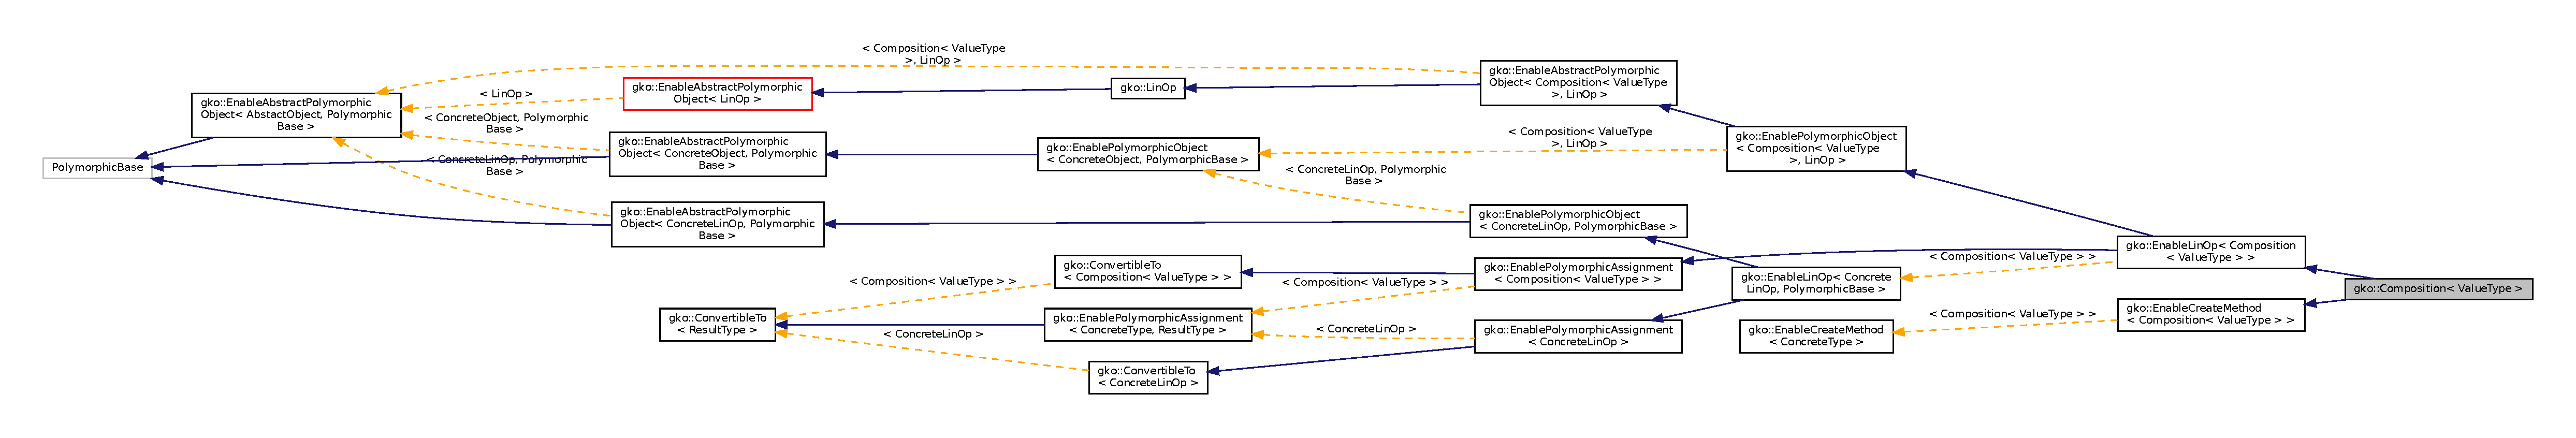
\includegraphics[width=350pt]{classgko_1_1Composition__coll__graph}
\end{center}
\end{figure}
\subsection*{Public Types}
\begin{DoxyCompactItemize}
\item 
\mbox{\Hypertarget{classgko_1_1Composition_ab565c6599fe56bf6b96f4c48f5992d6b}\label{classgko_1_1Composition_ab565c6599fe56bf6b96f4c48f5992d6b}} 
using {\bfseries value\+\_\+type} = Value\+Type
\end{DoxyCompactItemize}
\subsection*{Public Member Functions}
\begin{DoxyCompactItemize}
\item 
const std\+::vector$<$ std\+::shared\+\_\+ptr$<$ const \hyperlink{classgko_1_1LinOp}{Lin\+Op} $>$ $>$ \& \hyperlink{classgko_1_1Composition_a196507096c635aba24e1074050827c68}{get\+\_\+operators} () const noexcept
\begin{DoxyCompactList}\small\item\em Returns a list of operators of the composition. \end{DoxyCompactList}\end{DoxyCompactItemize}
\subsection*{Friends}
\begin{DoxyCompactItemize}
\item 
\mbox{\Hypertarget{classgko_1_1Composition_afa7c3f077edf67d0b19255dd78af3ecb}\label{classgko_1_1Composition_afa7c3f077edf67d0b19255dd78af3ecb}} 
class {\bfseries Enable\+Polymorphic\+Object$<$ Composition, Lin\+Op $>$}
\item 
\mbox{\Hypertarget{classgko_1_1Composition_a0350dc3dedd61760b46c3afd62943e6c}\label{classgko_1_1Composition_a0350dc3dedd61760b46c3afd62943e6c}} 
class {\bfseries Enable\+Create\+Method$<$ Composition $>$}
\end{DoxyCompactItemize}
\subsection*{Additional Inherited Members}


\subsection{Detailed Description}
\subsubsection*{template$<$typename Value\+Type = default\+\_\+precision$>$\newline
class gko\+::\+Composition$<$ Value\+Type $>$}

The \hyperlink{classgko_1_1Composition}{Composition} class can be used to compose linear operators {\ttfamily op1, op2, ..., opn} and obtain the operator `op1 $\ast$ op2 $\ast$ ... 


\begin{DoxyItemize}
\item opn`.
\end{DoxyItemize}


\begin{DoxyTemplParams}{Template Parameters}
{\em Value\+Type} & precision of input and result vectors \\
\hline
\end{DoxyTemplParams}


\subsection{Member Function Documentation}
\mbox{\Hypertarget{classgko_1_1Composition_a196507096c635aba24e1074050827c68}\label{classgko_1_1Composition_a196507096c635aba24e1074050827c68}} 
\index{gko\+::\+Composition@{gko\+::\+Composition}!get\+\_\+operators@{get\+\_\+operators}}
\index{get\+\_\+operators@{get\+\_\+operators}!gko\+::\+Composition@{gko\+::\+Composition}}
\subsubsection{\texorpdfstring{get\+\_\+operators()}{get\_operators()}}
{\footnotesize\ttfamily template$<$typename Value\+Type  = default\+\_\+precision$>$ \\
const std\+::vector$<$std\+::shared\+\_\+ptr$<$const \hyperlink{classgko_1_1LinOp}{Lin\+Op}$>$ $>$\& \hyperlink{classgko_1_1Composition}{gko\+::\+Composition}$<$ Value\+Type $>$\+::get\+\_\+operators (\begin{DoxyParamCaption}{ }\end{DoxyParamCaption}) const\hspace{0.3cm}{\ttfamily [inline]}, {\ttfamily [noexcept]}}



Returns a list of operators of the composition. 

\begin{DoxyReturn}{Returns}
a list of operators 
\end{DoxyReturn}


The documentation for this class was generated from the following file\+:\begin{DoxyCompactItemize}
\item 
ginkgo/core/base/composition.\+hpp (f9f0549a)\end{DoxyCompactItemize}

\hypertarget{structgko_1_1accessor_1_1conj__operaton}{}\section{gko\+:\+:accessor\+:\+:conj\+\_\+operaton$<$ Operand $>$ Struct Template Reference}
\label{structgko_1_1accessor_1_1conj__operaton}\index{gko\+::accessor\+::conj\+\_\+operaton$<$ Operand $>$@{gko\+::accessor\+::conj\+\_\+operaton$<$ Operand $>$}}


Collaboration diagram for gko\+:\+:accessor\+:\+:conj\+\_\+operaton$<$ Operand $>$\+:
\nopagebreak
\begin{figure}[H]
\begin{center}
\leavevmode
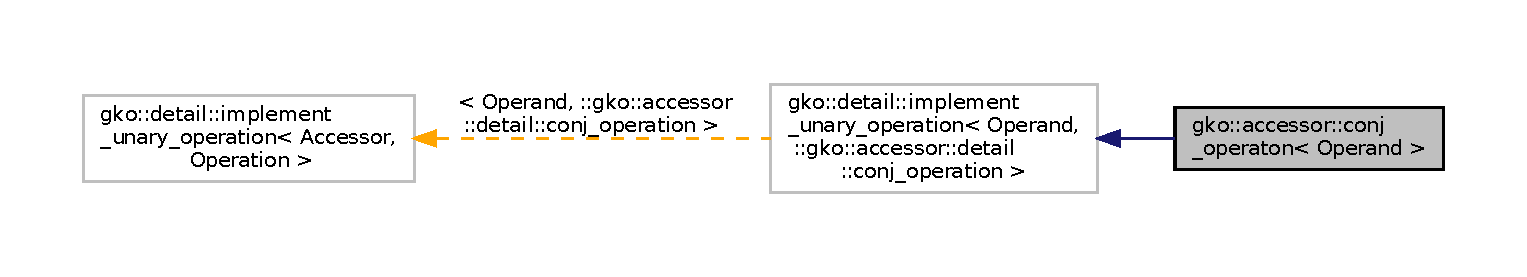
\includegraphics[width=350pt]{structgko_1_1accessor_1_1conj__operaton__coll__graph}
\end{center}
\end{figure}


The documentation for this struct was generated from the following file\+:\begin{DoxyCompactItemize}
\item 
ginkgo/core/base/range.\+hpp (c828dca0)\end{DoxyCompactItemize}

\hypertarget{classgko_1_1log_1_1Convergence}{}\section{gko\+:\+:log\+:\+:Convergence$<$ Value\+Type $>$ Class Template Reference}
\label{classgko_1_1log_1_1Convergence}\index{gko\+::log\+::\+Convergence$<$ Value\+Type $>$@{gko\+::log\+::\+Convergence$<$ Value\+Type $>$}}


\hyperlink{classgko_1_1log_1_1Convergence}{Convergence} is a \hyperlink{classgko_1_1log_1_1Logger}{Logger} which logs data strictly from the {\ttfamily criterion\+\_\+check\+\_\+completed} event.  




{\ttfamily \#include $<$ginkgo/core/log/convergence.\+hpp$>$}



Collaboration diagram for gko\+:\+:log\+:\+:Convergence$<$ Value\+Type $>$\+:
\nopagebreak
\begin{figure}[H]
\begin{center}
\leavevmode
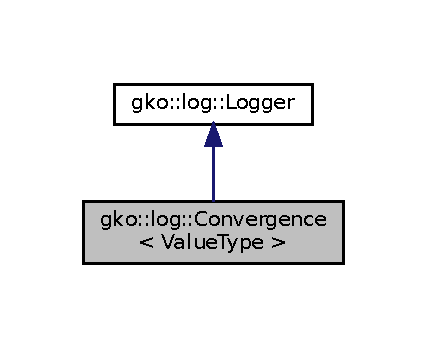
\includegraphics[width=205pt]{classgko_1_1log_1_1Convergence__coll__graph}
\end{center}
\end{figure}
\subsection*{Public Member Functions}
\begin{DoxyCompactItemize}
\item 
void \hyperlink{classgko_1_1log_1_1Convergence_ae20904a348216c22750c266372b07b6e}{on\+\_\+criterion\+\_\+check\+\_\+completed} (const \hyperlink{classgko_1_1stop_1_1Criterion}{stop\+::\+Criterion} $\ast$criterion, const \hyperlink{namespacegko_a6e5c95df0ae4e47aab2f604a22d98ee7}{size\+\_\+type} \&num\+\_\+iterations, const \hyperlink{classgko_1_1LinOp}{Lin\+Op} $\ast$residual, const \hyperlink{classgko_1_1LinOp}{Lin\+Op} $\ast$residual\+\_\+norm, const \hyperlink{classgko_1_1LinOp}{Lin\+Op} $\ast$solution, const \hyperlink{namespacegko_a3950fc3732811a8563484e5098c31531}{uint8} \&stopping\+\_\+id, const bool \&set\+\_\+finalized, const \hyperlink{classgko_1_1Array}{Array}$<$ \hyperlink{classgko_1_1stopping__status}{stopping\+\_\+status} $>$ $\ast$status, const bool \&one\+\_\+changed, const bool \&all\+\_\+converged) const override
\begin{DoxyCompactList}\small\item\em \hyperlink{classgko_1_1stop_1_1Criterion}{stop\+::\+Criterion}\textquotesingle{}s check completed event. \end{DoxyCompactList}\item 
const \hyperlink{namespacegko_a6e5c95df0ae4e47aab2f604a22d98ee7}{size\+\_\+type} \& \hyperlink{classgko_1_1log_1_1Convergence_ae4f2ae84d87df2bffa814f51a8f09793}{get\+\_\+num\+\_\+iterations} () const noexcept
\begin{DoxyCompactList}\small\item\em Returns the number of iterations. \end{DoxyCompactList}\item 
const \hyperlink{classgko_1_1LinOp}{Lin\+Op} $\ast$ \hyperlink{classgko_1_1log_1_1Convergence_a6595e7edae4cb080943493252b6d77e9}{get\+\_\+residual} () const noexcept
\begin{DoxyCompactList}\small\item\em Returns the residual. \end{DoxyCompactList}\item 
const \hyperlink{classgko_1_1LinOp}{Lin\+Op} $\ast$ \hyperlink{classgko_1_1log_1_1Convergence_a68297edb94aee77f6125c4b823f4503c}{get\+\_\+residual\+\_\+norm} () const noexcept
\begin{DoxyCompactList}\small\item\em Returns the residual norm. \end{DoxyCompactList}\end{DoxyCompactItemize}
\subsection*{Static Public Member Functions}
\begin{DoxyCompactItemize}
\item 
static std\+::unique\+\_\+ptr$<$ \hyperlink{classgko_1_1log_1_1Convergence}{Convergence} $>$ \hyperlink{classgko_1_1log_1_1Convergence_ad46f4f47f7392125e921d483a556017d}{create} (std\+::shared\+\_\+ptr$<$ const \hyperlink{classgko_1_1Executor}{Executor} $>$ exec, const mask\+\_\+type \&enabled\+\_\+events=\hyperlink{classgko_1_1log_1_1Logger_a02534863a2d2f92dfeb2c39038365532}{Logger\+::all\+\_\+events\+\_\+mask})
\begin{DoxyCompactList}\small\item\em Creates a convergence logger. \end{DoxyCompactList}\end{DoxyCompactItemize}
\subsection*{Additional Inherited Members}


\subsection{Detailed Description}
\subsubsection*{template$<$typename Value\+Type = default\+\_\+precision$>$\newline
class gko\+::log\+::\+Convergence$<$ Value\+Type $>$}

\hyperlink{classgko_1_1log_1_1Convergence}{Convergence} is a \hyperlink{classgko_1_1log_1_1Logger}{Logger} which logs data strictly from the {\ttfamily criterion\+\_\+check\+\_\+completed} event. 

The purpose of this logger is to give a simple access to standard data generated by the solver once it has converged with minimal overhead.

This logger also computes the residual norm from the residual when the residual norm was not available. This can add some slight overhead. 

\subsection{Member Function Documentation}
\mbox{\Hypertarget{classgko_1_1log_1_1Convergence_ad46f4f47f7392125e921d483a556017d}\label{classgko_1_1log_1_1Convergence_ad46f4f47f7392125e921d483a556017d}} 
\index{gko\+::log\+::\+Convergence@{gko\+::log\+::\+Convergence}!create@{create}}
\index{create@{create}!gko\+::log\+::\+Convergence@{gko\+::log\+::\+Convergence}}
\subsubsection{\texorpdfstring{create()}{create()}}
{\footnotesize\ttfamily template$<$typename Value\+Type  = default\+\_\+precision$>$ \\
static std\+::unique\+\_\+ptr$<$\hyperlink{classgko_1_1log_1_1Convergence}{Convergence}$>$ \hyperlink{classgko_1_1log_1_1Convergence}{gko\+::log\+::\+Convergence}$<$ Value\+Type $>$\+::create (\begin{DoxyParamCaption}\item[{std\+::shared\+\_\+ptr$<$ const \hyperlink{classgko_1_1Executor}{Executor} $>$}]{exec,  }\item[{const mask\+\_\+type \&}]{enabled\+\_\+events = {\ttfamily \hyperlink{classgko_1_1log_1_1Logger_a02534863a2d2f92dfeb2c39038365532}{Logger\+::all\+\_\+events\+\_\+mask}} }\end{DoxyParamCaption})\hspace{0.3cm}{\ttfamily [static]}}



Creates a convergence logger. 

This dynamically allocates the memory, constructs the object and returns an std\+::unique\+\_\+ptr to this object.


\begin{DoxyParams}{Parameters}
{\em exec} & the executor \\
\hline
{\em enabled\+\_\+events} & the events enabled for this logger. By default all events.\\
\hline
\end{DoxyParams}
\begin{DoxyReturn}{Returns}
an std\+::unique\+\_\+ptr to the the constructed object 
\end{DoxyReturn}
\mbox{\Hypertarget{classgko_1_1log_1_1Convergence_ae4f2ae84d87df2bffa814f51a8f09793}\label{classgko_1_1log_1_1Convergence_ae4f2ae84d87df2bffa814f51a8f09793}} 
\index{gko\+::log\+::\+Convergence@{gko\+::log\+::\+Convergence}!get\+\_\+num\+\_\+iterations@{get\+\_\+num\+\_\+iterations}}
\index{get\+\_\+num\+\_\+iterations@{get\+\_\+num\+\_\+iterations}!gko\+::log\+::\+Convergence@{gko\+::log\+::\+Convergence}}
\subsubsection{\texorpdfstring{get\+\_\+num\+\_\+iterations()}{get\_num\_iterations()}}
{\footnotesize\ttfamily template$<$typename Value\+Type  = default\+\_\+precision$>$ \\
const \hyperlink{namespacegko_a6e5c95df0ae4e47aab2f604a22d98ee7}{size\+\_\+type}\& \hyperlink{classgko_1_1log_1_1Convergence}{gko\+::log\+::\+Convergence}$<$ Value\+Type $>$\+::get\+\_\+num\+\_\+iterations (\begin{DoxyParamCaption}{ }\end{DoxyParamCaption}) const\hspace{0.3cm}{\ttfamily [noexcept]}}



Returns the number of iterations. 

\begin{DoxyReturn}{Returns}
the number of iterations 
\end{DoxyReturn}
\mbox{\Hypertarget{classgko_1_1log_1_1Convergence_a6595e7edae4cb080943493252b6d77e9}\label{classgko_1_1log_1_1Convergence_a6595e7edae4cb080943493252b6d77e9}} 
\index{gko\+::log\+::\+Convergence@{gko\+::log\+::\+Convergence}!get\+\_\+residual@{get\+\_\+residual}}
\index{get\+\_\+residual@{get\+\_\+residual}!gko\+::log\+::\+Convergence@{gko\+::log\+::\+Convergence}}
\subsubsection{\texorpdfstring{get\+\_\+residual()}{get\_residual()}}
{\footnotesize\ttfamily template$<$typename Value\+Type  = default\+\_\+precision$>$ \\
const \hyperlink{classgko_1_1LinOp}{Lin\+Op}$\ast$ \hyperlink{classgko_1_1log_1_1Convergence}{gko\+::log\+::\+Convergence}$<$ Value\+Type $>$\+::get\+\_\+residual (\begin{DoxyParamCaption}{ }\end{DoxyParamCaption}) const\hspace{0.3cm}{\ttfamily [noexcept]}}



Returns the residual. 

\begin{DoxyReturn}{Returns}
the residual 
\end{DoxyReturn}
\mbox{\Hypertarget{classgko_1_1log_1_1Convergence_a68297edb94aee77f6125c4b823f4503c}\label{classgko_1_1log_1_1Convergence_a68297edb94aee77f6125c4b823f4503c}} 
\index{gko\+::log\+::\+Convergence@{gko\+::log\+::\+Convergence}!get\+\_\+residual\+\_\+norm@{get\+\_\+residual\+\_\+norm}}
\index{get\+\_\+residual\+\_\+norm@{get\+\_\+residual\+\_\+norm}!gko\+::log\+::\+Convergence@{gko\+::log\+::\+Convergence}}
\subsubsection{\texorpdfstring{get\+\_\+residual\+\_\+norm()}{get\_residual\_norm()}}
{\footnotesize\ttfamily template$<$typename Value\+Type  = default\+\_\+precision$>$ \\
const \hyperlink{classgko_1_1LinOp}{Lin\+Op}$\ast$ \hyperlink{classgko_1_1log_1_1Convergence}{gko\+::log\+::\+Convergence}$<$ Value\+Type $>$\+::get\+\_\+residual\+\_\+norm (\begin{DoxyParamCaption}{ }\end{DoxyParamCaption}) const\hspace{0.3cm}{\ttfamily [noexcept]}}



Returns the residual norm. 

\begin{DoxyReturn}{Returns}
the residual norm 
\end{DoxyReturn}


References gko\+::log\+::\+Logger\+::all\+\_\+events\+\_\+mask.

\mbox{\Hypertarget{classgko_1_1log_1_1Convergence_ae20904a348216c22750c266372b07b6e}\label{classgko_1_1log_1_1Convergence_ae20904a348216c22750c266372b07b6e}} 
\index{gko\+::log\+::\+Convergence@{gko\+::log\+::\+Convergence}!on\+\_\+criterion\+\_\+check\+\_\+completed@{on\+\_\+criterion\+\_\+check\+\_\+completed}}
\index{on\+\_\+criterion\+\_\+check\+\_\+completed@{on\+\_\+criterion\+\_\+check\+\_\+completed}!gko\+::log\+::\+Convergence@{gko\+::log\+::\+Convergence}}
\subsubsection{\texorpdfstring{on\+\_\+criterion\+\_\+check\+\_\+completed()}{on\_criterion\_check\_completed()}}
{\footnotesize\ttfamily template$<$typename Value\+Type  = default\+\_\+precision$>$ \\
void \hyperlink{classgko_1_1log_1_1Convergence}{gko\+::log\+::\+Convergence}$<$ Value\+Type $>$\+::on\+\_\+criterion\+\_\+check\+\_\+completed (\begin{DoxyParamCaption}\item[{const \hyperlink{classgko_1_1stop_1_1Criterion}{stop\+::\+Criterion} $\ast$}]{criterion,  }\item[{const \hyperlink{namespacegko_a6e5c95df0ae4e47aab2f604a22d98ee7}{size\+\_\+type} \&}]{it,  }\item[{const \hyperlink{classgko_1_1LinOp}{Lin\+Op} $\ast$}]{r,  }\item[{const \hyperlink{classgko_1_1LinOp}{Lin\+Op} $\ast$}]{tau,  }\item[{const \hyperlink{classgko_1_1LinOp}{Lin\+Op} $\ast$}]{x,  }\item[{const \hyperlink{namespacegko_a3950fc3732811a8563484e5098c31531}{uint8} \&}]{stopping\+\_\+id,  }\item[{const bool \&}]{set\+\_\+finalized,  }\item[{const \hyperlink{classgko_1_1Array}{Array}$<$ \hyperlink{classgko_1_1stopping__status}{stopping\+\_\+status} $>$ $\ast$}]{status,  }\item[{const bool \&}]{one\+\_\+changed,  }\item[{const bool \&}]{all\+\_\+converged }\end{DoxyParamCaption}) const\hspace{0.3cm}{\ttfamily [override]}, {\ttfamily [virtual]}}



\hyperlink{classgko_1_1stop_1_1Criterion}{stop\+::\+Criterion}\textquotesingle{}s check completed event. 

Parameters are the Criterion, the stopping\+Id, the finalized boolean, the stopping status, plus the output one\+\_\+changed boolean and output all\+\_\+converged boolean.


\begin{DoxyParams}{Parameters}
{\em criterion} & the criterion used \\
\hline
{\em it} & the current iteration count \\
\hline
{\em r} & the residual \\
\hline
{\em tau} & the residual norm \\
\hline
{\em x} & the solution \\
\hline
{\em stopping\+\_\+id} & the id of the stopping criterion \\
\hline
{\em set\+\_\+finalized} & whether this finalizes the iteration \\
\hline
{\em status} & the stopping status of the right hand sides \\
\hline
{\em one\+\_\+changed} & whether at least one right hand side converged or not \\
\hline
{\em all\+\_\+converged} & whether all right hand sides \\
\hline
\end{DoxyParams}


Reimplemented from \hyperlink{classgko_1_1log_1_1Logger}{gko\+::log\+::\+Logger}.



The documentation for this class was generated from the following file\+:\begin{DoxyCompactItemize}
\item 
ginkgo/core/log/convergence.\+hpp (c828dca0)\end{DoxyCompactItemize}

\hypertarget{classgko_1_1ConvertibleTo}{}\doxysection{gko\+::Convertible\+To$<$ Result\+Type $>$ Class Template Reference}
\label{classgko_1_1ConvertibleTo}\index{gko::ConvertibleTo$<$ ResultType $>$@{gko::ConvertibleTo$<$ ResultType $>$}}


\mbox{\hyperlink{classgko_1_1ConvertibleTo}{Convertible\+To}} interface is used to mark that the implementer can be converted to the object of Result\+Type.  




{\ttfamily \#include $<$ginkgo/core/base/polymorphic\+\_\+object.\+hpp$>$}

\doxysubsection*{Public Types}
\begin{DoxyCompactItemize}
\item 
\mbox{\Hypertarget{classgko_1_1ConvertibleTo_a96d1c9f59700620c31fca1062f57de92}\label{classgko_1_1ConvertibleTo_a96d1c9f59700620c31fca1062f57de92}} 
using {\bfseries result\+\_\+type} = Result\+Type
\end{DoxyCompactItemize}
\doxysubsection*{Public Member Functions}
\begin{DoxyCompactItemize}
\item 
virtual void \mbox{\hyperlink{classgko_1_1ConvertibleTo_aa7f3420babcbed39ee15bc020bed4f7e}{convert\+\_\+to}} (result\+\_\+type $\ast$result) const =0
\begin{DoxyCompactList}\small\item\em Converts the implementer to an object of type result\+\_\+type. \end{DoxyCompactList}\item 
virtual void \mbox{\hyperlink{classgko_1_1ConvertibleTo_ab9047c7c49e0f83c79b54c0034d6197b}{move\+\_\+to}} (result\+\_\+type $\ast$result)=0
\begin{DoxyCompactList}\small\item\em Converts the implementer to an object of type result\+\_\+type by moving data from this object. \end{DoxyCompactList}\end{DoxyCompactItemize}


\doxysubsection{Detailed Description}
\subsubsection*{template$<$typename Result\+Type$>$\newline
class gko\+::\+Convertible\+To$<$ Result\+Type $>$}

\mbox{\hyperlink{classgko_1_1ConvertibleTo}{Convertible\+To}} interface is used to mark that the implementer can be converted to the object of Result\+Type. 

This interface is used to enable conversions between polymorphic objects. To mark that an object of type {\ttfamily U} can be converted to an object of type {\ttfamily V}, {\ttfamily U} should implement Convertible\+To$<$\+V$>$. Then, the implementation of {\ttfamily \mbox{\hyperlink{classgko_1_1PolymorphicObject_a5e6f713938293cfbe788d00480eb4d81}{Polymorphic\+Object\+::copy\+\_\+from}}} automatically generated by {\ttfamily \mbox{\hyperlink{classgko_1_1EnablePolymorphicObject}{Enable\+Polymorphic\+Object}}} mixin will use R\+T\+TI to figure out that {\ttfamily U} implements the interface and convert it using the convert\+\_\+to / move\+\_\+to methods of the interface.

As an example, the following function\+:


\begin{DoxyCode}{0}
\DoxyCodeLine{ \{c++\}}
\DoxyCodeLine{\textcolor{keywordtype}{void} my\_function(\textcolor{keyword}{const} U *u, V *v) \{}
\DoxyCodeLine{    v-\/>copy\_from(u);}
\DoxyCodeLine{\}}
\end{DoxyCode}


will convert object {\ttfamily u} to object {\ttfamily v} by checking that {\ttfamily u} can be dynamically casted to {\ttfamily \mbox{\hyperlink{classgko_1_1ConvertibleTo}{Convertible\+To}}\textbackslash{}$<$V\textbackslash{}$>$}, and calling \mbox{\hyperlink{classgko_1_1ConvertibleTo}{Convertible\+To}}$<$V$>$\+::convert\+\_\+to(\+V$\ast$)\`{} to do the actual conversion.

In case {\ttfamily u} is passed as a unique\+\_\+ptr, call to {\ttfamily convert\+\_\+to} will be replaced by a call to {\ttfamily move\+\_\+to} and trigger move semantics.


\begin{DoxyTemplParams}{Template Parameters}
{\em Result\+Type} & the type to which the implementer can be converted to, has to be a subclass of \mbox{\hyperlink{classgko_1_1PolymorphicObject}{Polymorphic\+Object}} \\
\hline
\end{DoxyTemplParams}


\doxysubsection{Member Function Documentation}
\mbox{\Hypertarget{classgko_1_1ConvertibleTo_aa7f3420babcbed39ee15bc020bed4f7e}\label{classgko_1_1ConvertibleTo_aa7f3420babcbed39ee15bc020bed4f7e}} 
\index{gko::ConvertibleTo$<$ ResultType $>$@{gko::ConvertibleTo$<$ ResultType $>$}!convert\_to@{convert\_to}}
\index{convert\_to@{convert\_to}!gko::ConvertibleTo$<$ ResultType $>$@{gko::ConvertibleTo$<$ ResultType $>$}}
\doxysubsubsection{\texorpdfstring{convert\_to()}{convert\_to()}}
{\footnotesize\ttfamily template$<$typename Result\+Type$>$ \\
virtual void \mbox{\hyperlink{classgko_1_1ConvertibleTo}{gko\+::\+Convertible\+To}}$<$ Result\+Type $>$\+::convert\+\_\+to (\begin{DoxyParamCaption}\item[{result\+\_\+type $\ast$}]{result }\end{DoxyParamCaption}) const\hspace{0.3cm}{\ttfamily [pure virtual]}}



Converts the implementer to an object of type result\+\_\+type. 


\begin{DoxyParams}{Parameters}
{\em result} & the object used to store the result of the conversion \\
\hline
\end{DoxyParams}


Implemented in \mbox{\hyperlink{classgko_1_1EnablePolymorphicAssignment_a6b7e6872e96084636f8ab5091063ada8}{gko\+::\+Enable\+Polymorphic\+Assignment$<$ Concrete\+Type, Result\+Type $>$}}, \mbox{\hyperlink{classgko_1_1EnablePolymorphicAssignment_a6b7e6872e96084636f8ab5091063ada8}{gko\+::\+Enable\+Polymorphic\+Assignment$<$ Sparsity\+Csr$<$ Value\+Type, Index\+Type $>$ $>$}}, \mbox{\hyperlink{classgko_1_1EnablePolymorphicAssignment_a6b7e6872e96084636f8ab5091063ada8}{gko\+::\+Enable\+Polymorphic\+Assignment$<$ Dense$<$ Value\+Type $>$ $>$}}, \mbox{\hyperlink{classgko_1_1EnablePolymorphicAssignment_a6b7e6872e96084636f8ab5091063ada8}{gko\+::\+Enable\+Polymorphic\+Assignment$<$ Upper\+Trs$<$ Value\+Type, Index\+Type $>$ $>$}}, \mbox{\hyperlink{classgko_1_1EnablePolymorphicAssignment_a6b7e6872e96084636f8ab5091063ada8}{gko\+::\+Enable\+Polymorphic\+Assignment$<$ Hybrid$<$ Value\+Type, Index\+Type $>$ $>$}}, \mbox{\hyperlink{classgko_1_1EnablePolymorphicAssignment_a6b7e6872e96084636f8ab5091063ada8}{gko\+::\+Enable\+Polymorphic\+Assignment$<$ Identity$<$ Value\+Type $>$ $>$}}, \mbox{\hyperlink{classgko_1_1EnablePolymorphicAssignment_a6b7e6872e96084636f8ab5091063ada8}{gko\+::\+Enable\+Polymorphic\+Assignment$<$ Concrete\+Lin\+Op $>$}}, \mbox{\hyperlink{classgko_1_1EnablePolymorphicAssignment_a6b7e6872e96084636f8ab5091063ada8}{gko\+::\+Enable\+Polymorphic\+Assignment$<$ Composition$<$ Value\+Type $>$ $>$}}, \mbox{\hyperlink{classgko_1_1EnablePolymorphicAssignment_a6b7e6872e96084636f8ab5091063ada8}{gko\+::\+Enable\+Polymorphic\+Assignment$<$ Bicgstab$<$ Value\+Type $>$ $>$}}, \mbox{\hyperlink{classgko_1_1EnablePolymorphicAssignment_a6b7e6872e96084636f8ab5091063ada8}{gko\+::\+Enable\+Polymorphic\+Assignment$<$ Lower\+Trs$<$ Value\+Type, Index\+Type $>$ $>$}}, \mbox{\hyperlink{classgko_1_1EnablePolymorphicAssignment_a6b7e6872e96084636f8ab5091063ada8}{gko\+::\+Enable\+Polymorphic\+Assignment$<$ Combination$<$ Value\+Type $>$ $>$}}, \mbox{\hyperlink{classgko_1_1EnablePolymorphicAssignment_a6b7e6872e96084636f8ab5091063ada8}{gko\+::\+Enable\+Polymorphic\+Assignment$<$ Gmres$<$ Value\+Type $>$ $>$}}, \mbox{\hyperlink{classgko_1_1EnablePolymorphicAssignment_a6b7e6872e96084636f8ab5091063ada8}{gko\+::\+Enable\+Polymorphic\+Assignment$<$ Csr$<$ Value\+Type, Index\+Type $>$ $>$}}, \mbox{\hyperlink{classgko_1_1EnablePolymorphicAssignment_a6b7e6872e96084636f8ab5091063ada8}{gko\+::\+Enable\+Polymorphic\+Assignment$<$ Ir$<$ Value\+Type $>$ $>$}}, \mbox{\hyperlink{classgko_1_1EnablePolymorphicAssignment_a6b7e6872e96084636f8ab5091063ada8}{gko\+::\+Enable\+Polymorphic\+Assignment$<$ Coo$<$ Value\+Type, Index\+Type $>$ $>$}}, \mbox{\hyperlink{classgko_1_1EnablePolymorphicAssignment_a6b7e6872e96084636f8ab5091063ada8}{gko\+::\+Enable\+Polymorphic\+Assignment$<$ Fcg$<$ Value\+Type $>$ $>$}}, \mbox{\hyperlink{classgko_1_1EnablePolymorphicAssignment_a6b7e6872e96084636f8ab5091063ada8}{gko\+::\+Enable\+Polymorphic\+Assignment$<$ Ilu$<$ L\+Solver\+Type, U\+Solver\+Type, Reverse\+Apply $>$ $>$}}, \mbox{\hyperlink{classgko_1_1EnablePolymorphicAssignment_a6b7e6872e96084636f8ab5091063ada8}{gko\+::\+Enable\+Polymorphic\+Assignment$<$ Concrete\+Factory $>$}}, \mbox{\hyperlink{classgko_1_1EnablePolymorphicAssignment_a6b7e6872e96084636f8ab5091063ada8}{gko\+::\+Enable\+Polymorphic\+Assignment$<$ Cgs$<$ Value\+Type $>$ $>$}}, \mbox{\hyperlink{classgko_1_1EnablePolymorphicAssignment_a6b7e6872e96084636f8ab5091063ada8}{gko\+::\+Enable\+Polymorphic\+Assignment$<$ Ell$<$ Value\+Type, Index\+Type $>$ $>$}}, \mbox{\hyperlink{classgko_1_1EnablePolymorphicAssignment_a6b7e6872e96084636f8ab5091063ada8}{gko\+::\+Enable\+Polymorphic\+Assignment$<$ Jacobi$<$ Value\+Type, Index\+Type $>$ $>$}}, \mbox{\hyperlink{classgko_1_1EnablePolymorphicAssignment_a6b7e6872e96084636f8ab5091063ada8}{gko\+::\+Enable\+Polymorphic\+Assignment$<$ Cg$<$ Value\+Type $>$ $>$}}, \mbox{\hyperlink{classgko_1_1EnablePolymorphicAssignment_a6b7e6872e96084636f8ab5091063ada8}{gko\+::\+Enable\+Polymorphic\+Assignment$<$ Sellp$<$ Value\+Type, Index\+Type $>$ $>$}}, \mbox{\hyperlink{classgko_1_1EnablePolymorphicAssignment_a6b7e6872e96084636f8ab5091063ada8}{gko\+::\+Enable\+Polymorphic\+Assignment$<$ Perturbation$<$ Value\+Type $>$ $>$}}, and \mbox{\hyperlink{classgko_1_1preconditioner_1_1Jacobi_a54ce952ac4a12c3f4686442375cd4dc8}{gko\+::preconditioner\+::\+Jacobi$<$ Value\+Type, Index\+Type $>$}}.

\mbox{\Hypertarget{classgko_1_1ConvertibleTo_ab9047c7c49e0f83c79b54c0034d6197b}\label{classgko_1_1ConvertibleTo_ab9047c7c49e0f83c79b54c0034d6197b}} 
\index{gko::ConvertibleTo$<$ ResultType $>$@{gko::ConvertibleTo$<$ ResultType $>$}!move\_to@{move\_to}}
\index{move\_to@{move\_to}!gko::ConvertibleTo$<$ ResultType $>$@{gko::ConvertibleTo$<$ ResultType $>$}}
\doxysubsubsection{\texorpdfstring{move\_to()}{move\_to()}}
{\footnotesize\ttfamily template$<$typename Result\+Type$>$ \\
virtual void \mbox{\hyperlink{classgko_1_1ConvertibleTo}{gko\+::\+Convertible\+To}}$<$ Result\+Type $>$\+::move\+\_\+to (\begin{DoxyParamCaption}\item[{result\+\_\+type $\ast$}]{result }\end{DoxyParamCaption})\hspace{0.3cm}{\ttfamily [pure virtual]}}



Converts the implementer to an object of type result\+\_\+type by moving data from this object. 

This method is used when the implementer is a temporary object, and move semantics can be used.


\begin{DoxyParams}{Parameters}
{\em result} & the object used to emplace the result of the conversion\\
\hline
\end{DoxyParams}
\begin{DoxyNote}{Note}
\mbox{\hyperlink{classgko_1_1ConvertibleTo_ab9047c7c49e0f83c79b54c0034d6197b}{Convertible\+To\+::move\+\_\+to}} can be implemented by simply calling \mbox{\hyperlink{classgko_1_1ConvertibleTo_aa7f3420babcbed39ee15bc020bed4f7e}{Convertible\+To\+::convert\+\_\+to}}. However, this operation can often be optimized by exploiting the fact that implementer\textquotesingle{}s data can be moved to the result. 
\end{DoxyNote}


Implemented in \mbox{\hyperlink{classgko_1_1EnablePolymorphicAssignment_a0a4cf244139e7761d6a91c61e029810e}{gko\+::\+Enable\+Polymorphic\+Assignment$<$ Concrete\+Type, Result\+Type $>$}}, \mbox{\hyperlink{classgko_1_1EnablePolymorphicAssignment_a0a4cf244139e7761d6a91c61e029810e}{gko\+::\+Enable\+Polymorphic\+Assignment$<$ Sparsity\+Csr$<$ Value\+Type, Index\+Type $>$ $>$}}, \mbox{\hyperlink{classgko_1_1EnablePolymorphicAssignment_a0a4cf244139e7761d6a91c61e029810e}{gko\+::\+Enable\+Polymorphic\+Assignment$<$ Dense$<$ Value\+Type $>$ $>$}}, \mbox{\hyperlink{classgko_1_1EnablePolymorphicAssignment_a0a4cf244139e7761d6a91c61e029810e}{gko\+::\+Enable\+Polymorphic\+Assignment$<$ Upper\+Trs$<$ Value\+Type, Index\+Type $>$ $>$}}, \mbox{\hyperlink{classgko_1_1EnablePolymorphicAssignment_a0a4cf244139e7761d6a91c61e029810e}{gko\+::\+Enable\+Polymorphic\+Assignment$<$ Hybrid$<$ Value\+Type, Index\+Type $>$ $>$}}, \mbox{\hyperlink{classgko_1_1EnablePolymorphicAssignment_a0a4cf244139e7761d6a91c61e029810e}{gko\+::\+Enable\+Polymorphic\+Assignment$<$ Identity$<$ Value\+Type $>$ $>$}}, \mbox{\hyperlink{classgko_1_1EnablePolymorphicAssignment_a0a4cf244139e7761d6a91c61e029810e}{gko\+::\+Enable\+Polymorphic\+Assignment$<$ Concrete\+Lin\+Op $>$}}, \mbox{\hyperlink{classgko_1_1EnablePolymorphicAssignment_a0a4cf244139e7761d6a91c61e029810e}{gko\+::\+Enable\+Polymorphic\+Assignment$<$ Composition$<$ Value\+Type $>$ $>$}}, \mbox{\hyperlink{classgko_1_1EnablePolymorphicAssignment_a0a4cf244139e7761d6a91c61e029810e}{gko\+::\+Enable\+Polymorphic\+Assignment$<$ Bicgstab$<$ Value\+Type $>$ $>$}}, \mbox{\hyperlink{classgko_1_1EnablePolymorphicAssignment_a0a4cf244139e7761d6a91c61e029810e}{gko\+::\+Enable\+Polymorphic\+Assignment$<$ Lower\+Trs$<$ Value\+Type, Index\+Type $>$ $>$}}, \mbox{\hyperlink{classgko_1_1EnablePolymorphicAssignment_a0a4cf244139e7761d6a91c61e029810e}{gko\+::\+Enable\+Polymorphic\+Assignment$<$ Combination$<$ Value\+Type $>$ $>$}}, \mbox{\hyperlink{classgko_1_1EnablePolymorphicAssignment_a0a4cf244139e7761d6a91c61e029810e}{gko\+::\+Enable\+Polymorphic\+Assignment$<$ Gmres$<$ Value\+Type $>$ $>$}}, \mbox{\hyperlink{classgko_1_1EnablePolymorphicAssignment_a0a4cf244139e7761d6a91c61e029810e}{gko\+::\+Enable\+Polymorphic\+Assignment$<$ Csr$<$ Value\+Type, Index\+Type $>$ $>$}}, \mbox{\hyperlink{classgko_1_1EnablePolymorphicAssignment_a0a4cf244139e7761d6a91c61e029810e}{gko\+::\+Enable\+Polymorphic\+Assignment$<$ Ir$<$ Value\+Type $>$ $>$}}, \mbox{\hyperlink{classgko_1_1EnablePolymorphicAssignment_a0a4cf244139e7761d6a91c61e029810e}{gko\+::\+Enable\+Polymorphic\+Assignment$<$ Coo$<$ Value\+Type, Index\+Type $>$ $>$}}, \mbox{\hyperlink{classgko_1_1EnablePolymorphicAssignment_a0a4cf244139e7761d6a91c61e029810e}{gko\+::\+Enable\+Polymorphic\+Assignment$<$ Fcg$<$ Value\+Type $>$ $>$}}, \mbox{\hyperlink{classgko_1_1EnablePolymorphicAssignment_a0a4cf244139e7761d6a91c61e029810e}{gko\+::\+Enable\+Polymorphic\+Assignment$<$ Ilu$<$ L\+Solver\+Type, U\+Solver\+Type, Reverse\+Apply $>$ $>$}}, \mbox{\hyperlink{classgko_1_1EnablePolymorphicAssignment_a0a4cf244139e7761d6a91c61e029810e}{gko\+::\+Enable\+Polymorphic\+Assignment$<$ Concrete\+Factory $>$}}, \mbox{\hyperlink{classgko_1_1EnablePolymorphicAssignment_a0a4cf244139e7761d6a91c61e029810e}{gko\+::\+Enable\+Polymorphic\+Assignment$<$ Cgs$<$ Value\+Type $>$ $>$}}, \mbox{\hyperlink{classgko_1_1EnablePolymorphicAssignment_a0a4cf244139e7761d6a91c61e029810e}{gko\+::\+Enable\+Polymorphic\+Assignment$<$ Ell$<$ Value\+Type, Index\+Type $>$ $>$}}, \mbox{\hyperlink{classgko_1_1EnablePolymorphicAssignment_a0a4cf244139e7761d6a91c61e029810e}{gko\+::\+Enable\+Polymorphic\+Assignment$<$ Jacobi$<$ Value\+Type, Index\+Type $>$ $>$}}, \mbox{\hyperlink{classgko_1_1EnablePolymorphicAssignment_a0a4cf244139e7761d6a91c61e029810e}{gko\+::\+Enable\+Polymorphic\+Assignment$<$ Cg$<$ Value\+Type $>$ $>$}}, \mbox{\hyperlink{classgko_1_1EnablePolymorphicAssignment_a0a4cf244139e7761d6a91c61e029810e}{gko\+::\+Enable\+Polymorphic\+Assignment$<$ Sellp$<$ Value\+Type, Index\+Type $>$ $>$}}, \mbox{\hyperlink{classgko_1_1EnablePolymorphicAssignment_a0a4cf244139e7761d6a91c61e029810e}{gko\+::\+Enable\+Polymorphic\+Assignment$<$ Perturbation$<$ Value\+Type $>$ $>$}}, and \mbox{\hyperlink{classgko_1_1preconditioner_1_1Jacobi_a6d5e28b3033772bfc6c96fbe3caca003}{gko\+::preconditioner\+::\+Jacobi$<$ Value\+Type, Index\+Type $>$}}.



The documentation for this class was generated from the following file\+:\begin{DoxyCompactItemize}
\item 
ginkgo/core/base/polymorphic\+\_\+object.\+hpp (3f08cf0a5)\end{DoxyCompactItemize}

\hypertarget{classgko_1_1matrix_1_1Coo}{}\doxysection{gko\+::matrix\+::Coo$<$ Value\+Type, Index\+Type $>$ Class Template Reference}
\label{classgko_1_1matrix_1_1Coo}\index{gko::matrix::Coo$<$ ValueType, IndexType $>$@{gko::matrix::Coo$<$ ValueType, IndexType $>$}}


C\+OO stores a matrix in the coordinate matrix format.  




{\ttfamily \#include $<$ginkgo/core/matrix/coo.\+hpp$>$}



Collaboration diagram for gko\+::matrix\+::Coo$<$ Value\+Type, Index\+Type $>$\+:
\nopagebreak
\begin{figure}[H]
\begin{center}
\leavevmode
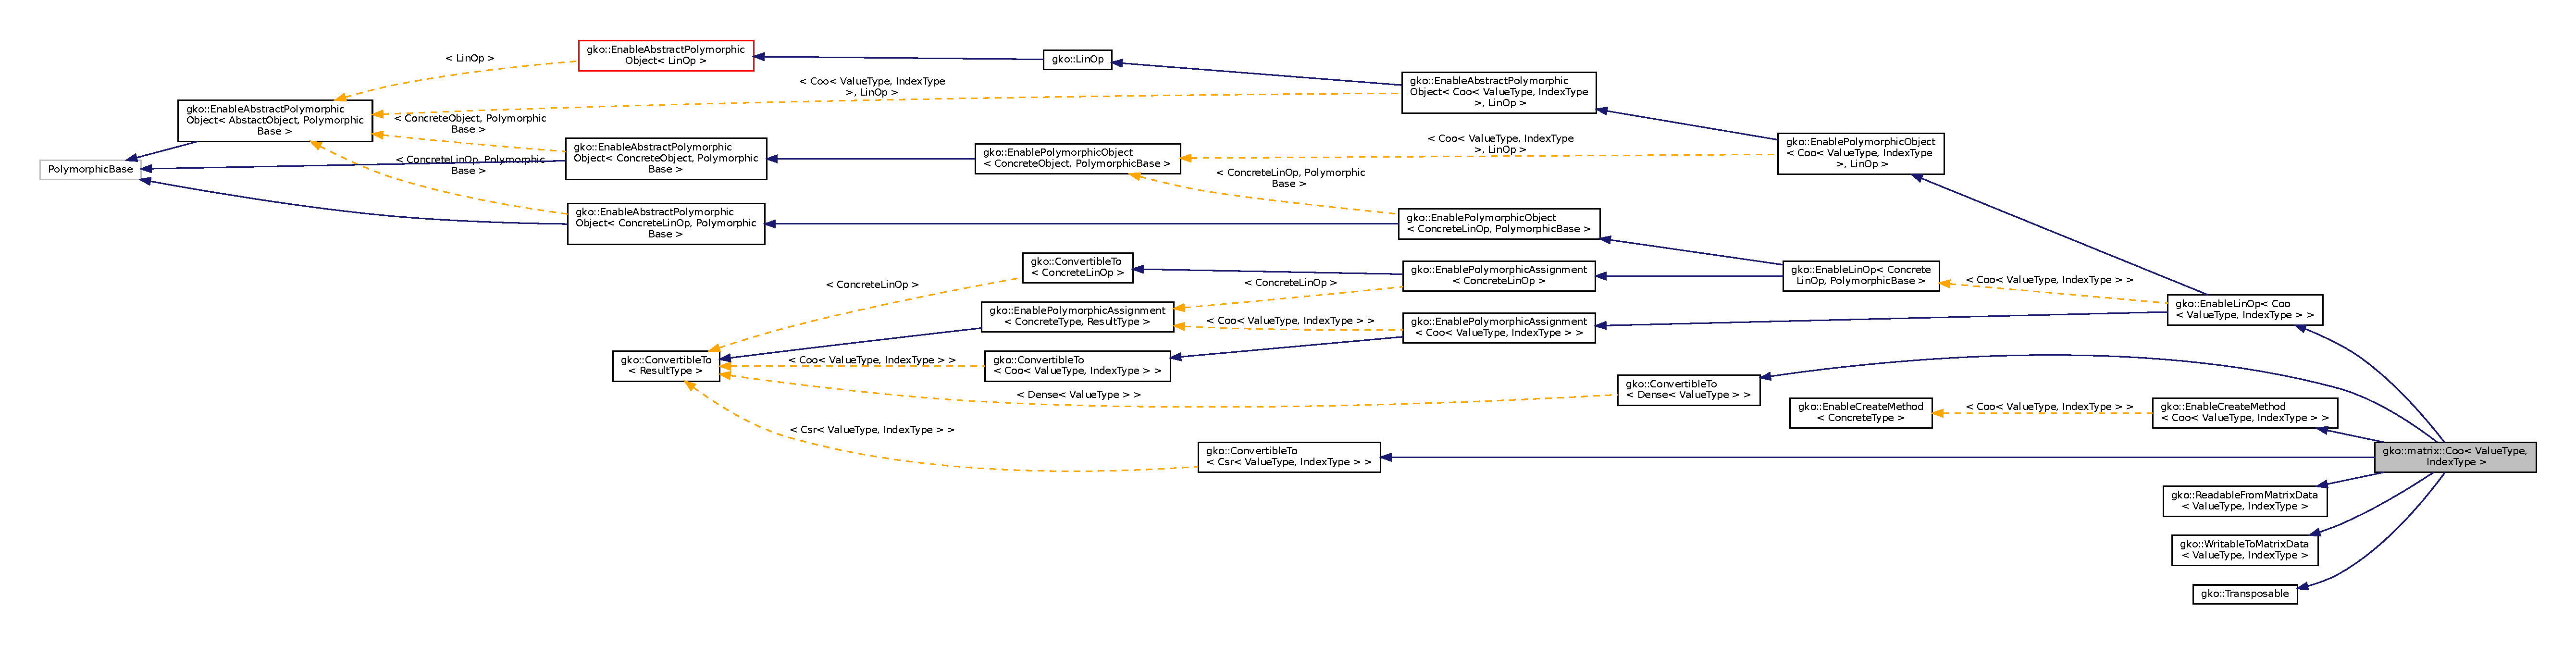
\includegraphics[width=350pt]{classgko_1_1matrix_1_1Coo__coll__graph}
\end{center}
\end{figure}
\doxysubsection*{Public Types}
\begin{DoxyCompactItemize}
\item 
\mbox{\Hypertarget{classgko_1_1matrix_1_1Coo_a4e3cdd13b760cf4816aef0d176551e99}\label{classgko_1_1matrix_1_1Coo_a4e3cdd13b760cf4816aef0d176551e99}} 
using {\bfseries value\+\_\+type} = Value\+Type
\item 
\mbox{\Hypertarget{classgko_1_1matrix_1_1Coo_ab7f7b99f477cfb086298104cf90105d2}\label{classgko_1_1matrix_1_1Coo_ab7f7b99f477cfb086298104cf90105d2}} 
using {\bfseries index\+\_\+type} = Index\+Type
\item 
\mbox{\Hypertarget{classgko_1_1matrix_1_1Coo_a52198fe6654bd0a2bec566a65bdc60ac}\label{classgko_1_1matrix_1_1Coo_a52198fe6654bd0a2bec566a65bdc60ac}} 
using {\bfseries mat\+\_\+data} = \mbox{\hyperlink{structgko_1_1matrix__data}{matrix\+\_\+data}}$<$ Value\+Type, Index\+Type $>$
\item 
\mbox{\Hypertarget{classgko_1_1matrix_1_1Coo_a70b752b84bc080854fb6e93b52e7735f}\label{classgko_1_1matrix_1_1Coo_a70b752b84bc080854fb6e93b52e7735f}} 
using {\bfseries absolute\+\_\+type} = \mbox{\hyperlink{namespacegko_afd46d554050c4ae90e84ea4fcd9a41f3}{remove\+\_\+complex}}$<$ \mbox{\hyperlink{classgko_1_1matrix_1_1Coo}{Coo}} $>$
\end{DoxyCompactItemize}
\doxysubsection*{Public Member Functions}
\begin{DoxyCompactItemize}
\item 
\mbox{\Hypertarget{classgko_1_1matrix_1_1Coo_a6fc91b35730bea0ea1b93e49a6b7343b}\label{classgko_1_1matrix_1_1Coo_a6fc91b35730bea0ea1b93e49a6b7343b}} 
void {\bfseries convert\+\_\+to} (\mbox{\hyperlink{classgko_1_1matrix_1_1Coo}{Coo}}$<$ \mbox{\hyperlink{namespacegko_a6362f751c7753cf4fa0a4771d56e8ede}{next\+\_\+precision}}$<$ Value\+Type $>$, Index\+Type $>$ $\ast$result) const override
\item 
\mbox{\Hypertarget{classgko_1_1matrix_1_1Coo_a7a14b90cb45223984a4601caa0341f4b}\label{classgko_1_1matrix_1_1Coo_a7a14b90cb45223984a4601caa0341f4b}} 
void {\bfseries move\+\_\+to} (\mbox{\hyperlink{classgko_1_1matrix_1_1Coo}{Coo}}$<$ \mbox{\hyperlink{namespacegko_a6362f751c7753cf4fa0a4771d56e8ede}{next\+\_\+precision}}$<$ Value\+Type $>$, Index\+Type $>$ $\ast$result) override
\item 
\mbox{\Hypertarget{classgko_1_1matrix_1_1Coo_a209277e9e7c7fe02c810524f758b96e0}\label{classgko_1_1matrix_1_1Coo_a209277e9e7c7fe02c810524f758b96e0}} 
void {\bfseries convert\+\_\+to} (\mbox{\hyperlink{classgko_1_1matrix_1_1Csr}{Csr}}$<$ Value\+Type, Index\+Type $>$ $\ast$other) const override
\item 
\mbox{\Hypertarget{classgko_1_1matrix_1_1Coo_a69d13086e01d54027191308f01fe7853}\label{classgko_1_1matrix_1_1Coo_a69d13086e01d54027191308f01fe7853}} 
void {\bfseries move\+\_\+to} (\mbox{\hyperlink{classgko_1_1matrix_1_1Csr}{Csr}}$<$ Value\+Type, Index\+Type $>$ $\ast$other) override
\item 
\mbox{\Hypertarget{classgko_1_1matrix_1_1Coo_afe1da5bbb43e64ced415d90b68e5d87d}\label{classgko_1_1matrix_1_1Coo_afe1da5bbb43e64ced415d90b68e5d87d}} 
void {\bfseries convert\+\_\+to} (\mbox{\hyperlink{classgko_1_1matrix_1_1Dense}{Dense}}$<$ Value\+Type $>$ $\ast$other) const override
\item 
\mbox{\Hypertarget{classgko_1_1matrix_1_1Coo_a0c4d89bb25548925ca9e698bdf00a946}\label{classgko_1_1matrix_1_1Coo_a0c4d89bb25548925ca9e698bdf00a946}} 
void {\bfseries move\+\_\+to} (\mbox{\hyperlink{classgko_1_1matrix_1_1Dense}{Dense}}$<$ Value\+Type $>$ $\ast$other) override
\item 
void \mbox{\hyperlink{classgko_1_1matrix_1_1Coo_ac0d4aeb19d9f55b62bea18bad1a408f5}{read}} (const \mbox{\hyperlink{structgko_1_1matrix__data}{mat\+\_\+data}} \&data) override
\begin{DoxyCompactList}\small\item\em Reads a matrix from a \mbox{\hyperlink{structgko_1_1matrix__data}{matrix\+\_\+data}} structure. \end{DoxyCompactList}\item 
void \mbox{\hyperlink{classgko_1_1matrix_1_1Coo_ae193466ca1a4a3c7d1383ddc5a2701ab}{write}} (\mbox{\hyperlink{structgko_1_1matrix__data}{mat\+\_\+data}} \&data) const override
\begin{DoxyCompactList}\small\item\em Writes a matrix to a \mbox{\hyperlink{structgko_1_1matrix__data}{matrix\+\_\+data}} structure. \end{DoxyCompactList}\item 
std\+::unique\+\_\+ptr$<$ \mbox{\hyperlink{classgko_1_1matrix_1_1Diagonal}{Diagonal}}$<$ Value\+Type $>$ $>$ \mbox{\hyperlink{classgko_1_1matrix_1_1Coo_a718eae56f6939543529ad5522d2d14e5}{extract\+\_\+diagonal}} () const override
\begin{DoxyCompactList}\small\item\em Extracts the diagonal entries of the matrix into a vector. \end{DoxyCompactList}\item 
std\+::unique\+\_\+ptr$<$ absolute\+\_\+type $>$ \mbox{\hyperlink{classgko_1_1matrix_1_1Coo_ab79b7f7b81b279774dd15edbd98965f1}{compute\+\_\+absolute}} () const override
\begin{DoxyCompactList}\small\item\em Gets the Absolute\+Lin\+Op. \end{DoxyCompactList}\item 
\mbox{\Hypertarget{classgko_1_1matrix_1_1Coo_aa3be345b0334650e50857c21837e0e07}\label{classgko_1_1matrix_1_1Coo_aa3be345b0334650e50857c21837e0e07}} 
void \mbox{\hyperlink{classgko_1_1matrix_1_1Coo_aa3be345b0334650e50857c21837e0e07}{compute\+\_\+absolute\+\_\+inplace}} () override
\begin{DoxyCompactList}\small\item\em Compute absolute inplace on each element. \end{DoxyCompactList}\item 
value\+\_\+type $\ast$ \mbox{\hyperlink{classgko_1_1matrix_1_1Coo_a1ce59517b8d6a8eeaacfed2b19d4057a}{get\+\_\+values}} () noexcept
\begin{DoxyCompactList}\small\item\em Returns the values of the matrix. \end{DoxyCompactList}\item 
const value\+\_\+type $\ast$ \mbox{\hyperlink{classgko_1_1matrix_1_1Coo_af0f6fe19d81bc4207aad66376f9c87c5}{get\+\_\+const\+\_\+values}} () const noexcept
\begin{DoxyCompactList}\small\item\em Returns the values of the matrix. \end{DoxyCompactList}\item 
index\+\_\+type $\ast$ \mbox{\hyperlink{classgko_1_1matrix_1_1Coo_a1b619cf23c7c87cb4109432c8e8db66d}{get\+\_\+col\+\_\+idxs}} () noexcept
\begin{DoxyCompactList}\small\item\em Returns the column indexes of the matrix. \end{DoxyCompactList}\item 
const index\+\_\+type $\ast$ \mbox{\hyperlink{classgko_1_1matrix_1_1Coo_ae4afdbf2dc5a5a42a197f3a479febc75}{get\+\_\+const\+\_\+col\+\_\+idxs}} () const noexcept
\begin{DoxyCompactList}\small\item\em Returns the column indexes of the matrix. \end{DoxyCompactList}\item 
index\+\_\+type $\ast$ \mbox{\hyperlink{classgko_1_1matrix_1_1Coo_a57aa0f7b701020c4322a3aed63d8a25d}{get\+\_\+row\+\_\+idxs}} () noexcept
\begin{DoxyCompactList}\small\item\em Returns the row indexes of the matrix. \end{DoxyCompactList}\item 
const index\+\_\+type $\ast$ \mbox{\hyperlink{classgko_1_1matrix_1_1Coo_a0fe0f33bf492bf2f9134927c7ee90e81}{get\+\_\+const\+\_\+row\+\_\+idxs}} () const noexcept
\item 
\mbox{\hyperlink{namespacegko_a6e5c95df0ae4e47aab2f604a22d98ee7}{size\+\_\+type}} \mbox{\hyperlink{classgko_1_1matrix_1_1Coo_aece531e069f8490fd8d2b3ab58f72d09}{get\+\_\+num\+\_\+stored\+\_\+elements}} () const noexcept
\begin{DoxyCompactList}\small\item\em Returns the number of elements explicitly stored in the matrix. \end{DoxyCompactList}\item 
\mbox{\hyperlink{classgko_1_1LinOp}{Lin\+Op}} $\ast$ \mbox{\hyperlink{classgko_1_1matrix_1_1Coo_ad2e97eee0ad21f8896f4a82cc5ac8a50}{apply2}} (const \mbox{\hyperlink{classgko_1_1LinOp}{Lin\+Op}} $\ast$b, \mbox{\hyperlink{classgko_1_1LinOp}{Lin\+Op}} $\ast$x)
\begin{DoxyCompactList}\small\item\em Applies \mbox{\hyperlink{classgko_1_1matrix_1_1Coo}{Coo}} matrix axpy to a vector (or a sequence of vectors). \end{DoxyCompactList}\item 
const \mbox{\hyperlink{classgko_1_1LinOp}{Lin\+Op}} $\ast$ \mbox{\hyperlink{classgko_1_1matrix_1_1Coo_a48b3fd46edc8b1770f2800e94871eb41}{apply2}} (const \mbox{\hyperlink{classgko_1_1LinOp}{Lin\+Op}} $\ast$b, \mbox{\hyperlink{classgko_1_1LinOp}{Lin\+Op}} $\ast$x) const
\item 
\mbox{\hyperlink{classgko_1_1LinOp}{Lin\+Op}} $\ast$ \mbox{\hyperlink{classgko_1_1matrix_1_1Coo_a549dafbe9245e3fcef3b02c4d6914c84}{apply2}} (const \mbox{\hyperlink{classgko_1_1LinOp}{Lin\+Op}} $\ast$alpha, const \mbox{\hyperlink{classgko_1_1LinOp}{Lin\+Op}} $\ast$b, \mbox{\hyperlink{classgko_1_1LinOp}{Lin\+Op}} $\ast$x)
\begin{DoxyCompactList}\small\item\em Performs the operation x = alpha $\ast$ \mbox{\hyperlink{classgko_1_1matrix_1_1Coo}{Coo}} $\ast$ b + x. \end{DoxyCompactList}\item 
const \mbox{\hyperlink{classgko_1_1LinOp}{Lin\+Op}} $\ast$ \mbox{\hyperlink{classgko_1_1matrix_1_1Coo_a05062dbf88132edf3a13d23783a8b07d}{apply2}} (const \mbox{\hyperlink{classgko_1_1LinOp}{Lin\+Op}} $\ast$alpha, const \mbox{\hyperlink{classgko_1_1LinOp}{Lin\+Op}} $\ast$b, \mbox{\hyperlink{classgko_1_1LinOp}{Lin\+Op}} $\ast$x) const
\begin{DoxyCompactList}\small\item\em Performs the operation x = alpha $\ast$ \mbox{\hyperlink{classgko_1_1matrix_1_1Coo}{Coo}} $\ast$ b + x. \end{DoxyCompactList}\end{DoxyCompactItemize}
\doxysubsection*{Friends}
\begin{DoxyCompactItemize}
\item 
\mbox{\Hypertarget{classgko_1_1matrix_1_1Coo_a7b73c83603cbcededd15ded9a873ea33}\label{classgko_1_1matrix_1_1Coo_a7b73c83603cbcededd15ded9a873ea33}} 
class {\bfseries Enable\+Create\+Method$<$ Coo $>$}
\item 
\mbox{\Hypertarget{classgko_1_1matrix_1_1Coo_a29c635db859b174df4d1cdc8be3ff2be}\label{classgko_1_1matrix_1_1Coo_a29c635db859b174df4d1cdc8be3ff2be}} 
class {\bfseries Enable\+Polymorphic\+Object$<$ Coo, Lin\+Op $>$}
\item 
\mbox{\Hypertarget{classgko_1_1matrix_1_1Coo_a3962faf971a3df6ff4c9226c61fb24cc}\label{classgko_1_1matrix_1_1Coo_a3962faf971a3df6ff4c9226c61fb24cc}} 
class {\bfseries Csr$<$ Value\+Type, Index\+Type $>$}
\item 
\mbox{\Hypertarget{classgko_1_1matrix_1_1Coo_a22a84c8f67f946aa60a2fa8bf5835a32}\label{classgko_1_1matrix_1_1Coo_a22a84c8f67f946aa60a2fa8bf5835a32}} 
class {\bfseries Dense$<$ Value\+Type $>$}
\item 
\mbox{\Hypertarget{classgko_1_1matrix_1_1Coo_a52291b122923e4e6e062cb896c14ecc3}\label{classgko_1_1matrix_1_1Coo_a52291b122923e4e6e062cb896c14ecc3}} 
class {\bfseries Coo\+Builder$<$ Value\+Type, Index\+Type $>$}
\item 
\mbox{\Hypertarget{classgko_1_1matrix_1_1Coo_ac0722b28c665c408a55adff82cce5a4b}\label{classgko_1_1matrix_1_1Coo_ac0722b28c665c408a55adff82cce5a4b}} 
class {\bfseries Coo$<$ to\+\_\+complex$<$ Value\+Type $>$, Index\+Type $>$}
\item 
\mbox{\Hypertarget{classgko_1_1matrix_1_1Coo_a12deb8a1b944cf409ac6e85151db2c25}\label{classgko_1_1matrix_1_1Coo_a12deb8a1b944cf409ac6e85151db2c25}} 
class {\bfseries Coo$<$ next\+\_\+precision$<$ Value\+Type $>$, Index\+Type $>$}
\end{DoxyCompactItemize}
\doxysubsection*{Additional Inherited Members}


\doxysubsection{Detailed Description}
\subsubsection*{template$<$typename Value\+Type = default\+\_\+precision, typename Index\+Type = int32$>$\newline
class gko\+::matrix\+::\+Coo$<$ Value\+Type, Index\+Type $>$}

C\+OO stores a matrix in the coordinate matrix format. 

The nonzero elements are stored in an array row-\/wise (but not neccessarily sorted by column index within a row). Two extra arrays contain the row and column indexes of each nonzero element of the matrix.


\begin{DoxyTemplParams}{Template Parameters}
{\em Value\+Type} & precision of matrix elements \\
\hline
{\em Index\+Type} & precision of matrix indexes \\
\hline
\end{DoxyTemplParams}


\doxysubsection{Member Function Documentation}
\mbox{\Hypertarget{classgko_1_1matrix_1_1Coo_a549dafbe9245e3fcef3b02c4d6914c84}\label{classgko_1_1matrix_1_1Coo_a549dafbe9245e3fcef3b02c4d6914c84}} 
\index{gko::matrix::Coo$<$ ValueType, IndexType $>$@{gko::matrix::Coo$<$ ValueType, IndexType $>$}!apply2@{apply2}}
\index{apply2@{apply2}!gko::matrix::Coo$<$ ValueType, IndexType $>$@{gko::matrix::Coo$<$ ValueType, IndexType $>$}}
\doxysubsubsection{\texorpdfstring{apply2()}{apply2()}\hspace{0.1cm}{\footnotesize\ttfamily [1/4]}}
{\footnotesize\ttfamily template$<$typename Value\+Type = default\+\_\+precision, typename Index\+Type = int32$>$ \\
\mbox{\hyperlink{classgko_1_1LinOp}{Lin\+Op}}$\ast$ \mbox{\hyperlink{classgko_1_1matrix_1_1Coo}{gko\+::matrix\+::\+Coo}}$<$ Value\+Type, Index\+Type $>$\+::apply2 (\begin{DoxyParamCaption}\item[{const \mbox{\hyperlink{classgko_1_1LinOp}{Lin\+Op}} $\ast$}]{alpha,  }\item[{const \mbox{\hyperlink{classgko_1_1LinOp}{Lin\+Op}} $\ast$}]{b,  }\item[{\mbox{\hyperlink{classgko_1_1LinOp}{Lin\+Op}} $\ast$}]{x }\end{DoxyParamCaption})\hspace{0.3cm}{\ttfamily [inline]}}



Performs the operation x = alpha $\ast$ \mbox{\hyperlink{classgko_1_1matrix_1_1Coo}{Coo}} $\ast$ b + x. 


\begin{DoxyParams}{Parameters}
{\em alpha} & scaling of the result of \mbox{\hyperlink{classgko_1_1matrix_1_1Coo}{Coo}} $\ast$ b \\
\hline
{\em b} & vector(s) on which the operator is applied \\
\hline
{\em x} & output vector(s)\\
\hline
\end{DoxyParams}
\begin{DoxyReturn}{Returns}
this 
\end{DoxyReturn}


References gko\+::\+Polymorphic\+Object\+::get\+\_\+executor(), and gko\+::make\+\_\+temporary\+\_\+clone().

\mbox{\Hypertarget{classgko_1_1matrix_1_1Coo_a05062dbf88132edf3a13d23783a8b07d}\label{classgko_1_1matrix_1_1Coo_a05062dbf88132edf3a13d23783a8b07d}} 
\index{gko::matrix::Coo$<$ ValueType, IndexType $>$@{gko::matrix::Coo$<$ ValueType, IndexType $>$}!apply2@{apply2}}
\index{apply2@{apply2}!gko::matrix::Coo$<$ ValueType, IndexType $>$@{gko::matrix::Coo$<$ ValueType, IndexType $>$}}
\doxysubsubsection{\texorpdfstring{apply2()}{apply2()}\hspace{0.1cm}{\footnotesize\ttfamily [2/4]}}
{\footnotesize\ttfamily template$<$typename Value\+Type = default\+\_\+precision, typename Index\+Type = int32$>$ \\
const \mbox{\hyperlink{classgko_1_1LinOp}{Lin\+Op}}$\ast$ \mbox{\hyperlink{classgko_1_1matrix_1_1Coo}{gko\+::matrix\+::\+Coo}}$<$ Value\+Type, Index\+Type $>$\+::apply2 (\begin{DoxyParamCaption}\item[{const \mbox{\hyperlink{classgko_1_1LinOp}{Lin\+Op}} $\ast$}]{alpha,  }\item[{const \mbox{\hyperlink{classgko_1_1LinOp}{Lin\+Op}} $\ast$}]{b,  }\item[{\mbox{\hyperlink{classgko_1_1LinOp}{Lin\+Op}} $\ast$}]{x }\end{DoxyParamCaption}) const\hspace{0.3cm}{\ttfamily [inline]}}



Performs the operation x = alpha $\ast$ \mbox{\hyperlink{classgko_1_1matrix_1_1Coo}{Coo}} $\ast$ b + x. 


\begin{DoxyParams}{Parameters}
{\em alpha} & scaling of the result of \mbox{\hyperlink{classgko_1_1matrix_1_1Coo}{Coo}} $\ast$ b \\
\hline
{\em b} & vector(s) on which the operator is applied \\
\hline
{\em x} & output vector(s)\\
\hline
\end{DoxyParams}
\begin{DoxyReturn}{Returns}
this 
\end{DoxyReturn}


References gko\+::\+Polymorphic\+Object\+::get\+\_\+executor(), and gko\+::make\+\_\+temporary\+\_\+clone().

\mbox{\Hypertarget{classgko_1_1matrix_1_1Coo_ad2e97eee0ad21f8896f4a82cc5ac8a50}\label{classgko_1_1matrix_1_1Coo_ad2e97eee0ad21f8896f4a82cc5ac8a50}} 
\index{gko::matrix::Coo$<$ ValueType, IndexType $>$@{gko::matrix::Coo$<$ ValueType, IndexType $>$}!apply2@{apply2}}
\index{apply2@{apply2}!gko::matrix::Coo$<$ ValueType, IndexType $>$@{gko::matrix::Coo$<$ ValueType, IndexType $>$}}
\doxysubsubsection{\texorpdfstring{apply2()}{apply2()}\hspace{0.1cm}{\footnotesize\ttfamily [3/4]}}
{\footnotesize\ttfamily template$<$typename Value\+Type = default\+\_\+precision, typename Index\+Type = int32$>$ \\
\mbox{\hyperlink{classgko_1_1LinOp}{Lin\+Op}}$\ast$ \mbox{\hyperlink{classgko_1_1matrix_1_1Coo}{gko\+::matrix\+::\+Coo}}$<$ Value\+Type, Index\+Type $>$\+::apply2 (\begin{DoxyParamCaption}\item[{const \mbox{\hyperlink{classgko_1_1LinOp}{Lin\+Op}} $\ast$}]{b,  }\item[{\mbox{\hyperlink{classgko_1_1LinOp}{Lin\+Op}} $\ast$}]{x }\end{DoxyParamCaption})\hspace{0.3cm}{\ttfamily [inline]}}



Applies \mbox{\hyperlink{classgko_1_1matrix_1_1Coo}{Coo}} matrix axpy to a vector (or a sequence of vectors). 

Performs the operation x = \mbox{\hyperlink{classgko_1_1matrix_1_1Coo}{Coo}} $\ast$ b + x


\begin{DoxyParams}{Parameters}
{\em b} & the input vector(s) on which the operator is applied \\
\hline
{\em x} & the output vector(s) where the result is stored\\
\hline
\end{DoxyParams}
\begin{DoxyReturn}{Returns}
this 
\end{DoxyReturn}


References gko\+::\+Polymorphic\+Object\+::get\+\_\+executor(), and gko\+::make\+\_\+temporary\+\_\+clone().

\mbox{\Hypertarget{classgko_1_1matrix_1_1Coo_a48b3fd46edc8b1770f2800e94871eb41}\label{classgko_1_1matrix_1_1Coo_a48b3fd46edc8b1770f2800e94871eb41}} 
\index{gko::matrix::Coo$<$ ValueType, IndexType $>$@{gko::matrix::Coo$<$ ValueType, IndexType $>$}!apply2@{apply2}}
\index{apply2@{apply2}!gko::matrix::Coo$<$ ValueType, IndexType $>$@{gko::matrix::Coo$<$ ValueType, IndexType $>$}}
\doxysubsubsection{\texorpdfstring{apply2()}{apply2()}\hspace{0.1cm}{\footnotesize\ttfamily [4/4]}}
{\footnotesize\ttfamily template$<$typename Value\+Type = default\+\_\+precision, typename Index\+Type = int32$>$ \\
const \mbox{\hyperlink{classgko_1_1LinOp}{Lin\+Op}}$\ast$ \mbox{\hyperlink{classgko_1_1matrix_1_1Coo}{gko\+::matrix\+::\+Coo}}$<$ Value\+Type, Index\+Type $>$\+::apply2 (\begin{DoxyParamCaption}\item[{const \mbox{\hyperlink{classgko_1_1LinOp}{Lin\+Op}} $\ast$}]{b,  }\item[{\mbox{\hyperlink{classgko_1_1LinOp}{Lin\+Op}} $\ast$}]{x }\end{DoxyParamCaption}) const\hspace{0.3cm}{\ttfamily [inline]}}







References gko\+::\+Polymorphic\+Object\+::get\+\_\+executor(), and gko\+::make\+\_\+temporary\+\_\+clone().

\mbox{\Hypertarget{classgko_1_1matrix_1_1Coo_ab79b7f7b81b279774dd15edbd98965f1}\label{classgko_1_1matrix_1_1Coo_ab79b7f7b81b279774dd15edbd98965f1}} 
\index{gko::matrix::Coo$<$ ValueType, IndexType $>$@{gko::matrix::Coo$<$ ValueType, IndexType $>$}!compute\_absolute@{compute\_absolute}}
\index{compute\_absolute@{compute\_absolute}!gko::matrix::Coo$<$ ValueType, IndexType $>$@{gko::matrix::Coo$<$ ValueType, IndexType $>$}}
\doxysubsubsection{\texorpdfstring{compute\_absolute()}{compute\_absolute()}}
{\footnotesize\ttfamily template$<$typename Value\+Type = default\+\_\+precision, typename Index\+Type = int32$>$ \\
std\+::unique\+\_\+ptr$<$absolute\+\_\+type$>$ \mbox{\hyperlink{classgko_1_1matrix_1_1Coo}{gko\+::matrix\+::\+Coo}}$<$ Value\+Type, Index\+Type $>$\+::compute\+\_\+absolute (\begin{DoxyParamCaption}{ }\end{DoxyParamCaption}) const\hspace{0.3cm}{\ttfamily [override]}, {\ttfamily [virtual]}}



Gets the Absolute\+Lin\+Op. 

\begin{DoxyReturn}{Returns}
a pointer to the new absolute object 
\end{DoxyReturn}


Implements \mbox{\hyperlink{classgko_1_1EnableAbsoluteComputation_ac30ab2b34bfa3e28e3324cb46f5f030a}{gko\+::\+Enable\+Absolute\+Computation$<$ remove\+\_\+complex$<$ Coo$<$ Value\+Type, Index\+Type $>$ $>$ $>$}}.

\mbox{\Hypertarget{classgko_1_1matrix_1_1Coo_a718eae56f6939543529ad5522d2d14e5}\label{classgko_1_1matrix_1_1Coo_a718eae56f6939543529ad5522d2d14e5}} 
\index{gko::matrix::Coo$<$ ValueType, IndexType $>$@{gko::matrix::Coo$<$ ValueType, IndexType $>$}!extract\_diagonal@{extract\_diagonal}}
\index{extract\_diagonal@{extract\_diagonal}!gko::matrix::Coo$<$ ValueType, IndexType $>$@{gko::matrix::Coo$<$ ValueType, IndexType $>$}}
\doxysubsubsection{\texorpdfstring{extract\_diagonal()}{extract\_diagonal()}}
{\footnotesize\ttfamily template$<$typename Value\+Type = default\+\_\+precision, typename Index\+Type = int32$>$ \\
std\+::unique\+\_\+ptr$<$\mbox{\hyperlink{classgko_1_1matrix_1_1Diagonal}{Diagonal}}$<$Value\+Type$>$ $>$ \mbox{\hyperlink{classgko_1_1matrix_1_1Coo}{gko\+::matrix\+::\+Coo}}$<$ Value\+Type, Index\+Type $>$\+::extract\+\_\+diagonal (\begin{DoxyParamCaption}{ }\end{DoxyParamCaption}) const\hspace{0.3cm}{\ttfamily [override]}, {\ttfamily [virtual]}}



Extracts the diagonal entries of the matrix into a vector. 


\begin{DoxyParams}{Parameters}
{\em diag} & the vector into which the diagonal will be written \\
\hline
\end{DoxyParams}


Implements \mbox{\hyperlink{classgko_1_1DiagonalExtractable_a3a748eb3a1ced4e679b67a0e20f46336}{gko\+::\+Diagonal\+Extractable$<$ Value\+Type $>$}}.

\mbox{\Hypertarget{classgko_1_1matrix_1_1Coo_a1b619cf23c7c87cb4109432c8e8db66d}\label{classgko_1_1matrix_1_1Coo_a1b619cf23c7c87cb4109432c8e8db66d}} 
\index{gko::matrix::Coo$<$ ValueType, IndexType $>$@{gko::matrix::Coo$<$ ValueType, IndexType $>$}!get\_col\_idxs@{get\_col\_idxs}}
\index{get\_col\_idxs@{get\_col\_idxs}!gko::matrix::Coo$<$ ValueType, IndexType $>$@{gko::matrix::Coo$<$ ValueType, IndexType $>$}}
\doxysubsubsection{\texorpdfstring{get\_col\_idxs()}{get\_col\_idxs()}}
{\footnotesize\ttfamily template$<$typename Value\+Type = default\+\_\+precision, typename Index\+Type = int32$>$ \\
index\+\_\+type$\ast$ \mbox{\hyperlink{classgko_1_1matrix_1_1Coo}{gko\+::matrix\+::\+Coo}}$<$ Value\+Type, Index\+Type $>$\+::get\+\_\+col\+\_\+idxs (\begin{DoxyParamCaption}{ }\end{DoxyParamCaption})\hspace{0.3cm}{\ttfamily [inline]}, {\ttfamily [noexcept]}}



Returns the column indexes of the matrix. 

\begin{DoxyReturn}{Returns}
the column indexes of the matrix. 
\end{DoxyReturn}


References gko\+::\+Array$<$ Value\+Type $>$\+::get\+\_\+data().

\mbox{\Hypertarget{classgko_1_1matrix_1_1Coo_ae4afdbf2dc5a5a42a197f3a479febc75}\label{classgko_1_1matrix_1_1Coo_ae4afdbf2dc5a5a42a197f3a479febc75}} 
\index{gko::matrix::Coo$<$ ValueType, IndexType $>$@{gko::matrix::Coo$<$ ValueType, IndexType $>$}!get\_const\_col\_idxs@{get\_const\_col\_idxs}}
\index{get\_const\_col\_idxs@{get\_const\_col\_idxs}!gko::matrix::Coo$<$ ValueType, IndexType $>$@{gko::matrix::Coo$<$ ValueType, IndexType $>$}}
\doxysubsubsection{\texorpdfstring{get\_const\_col\_idxs()}{get\_const\_col\_idxs()}}
{\footnotesize\ttfamily template$<$typename Value\+Type = default\+\_\+precision, typename Index\+Type = int32$>$ \\
const index\+\_\+type$\ast$ \mbox{\hyperlink{classgko_1_1matrix_1_1Coo}{gko\+::matrix\+::\+Coo}}$<$ Value\+Type, Index\+Type $>$\+::get\+\_\+const\+\_\+col\+\_\+idxs (\begin{DoxyParamCaption}{ }\end{DoxyParamCaption}) const\hspace{0.3cm}{\ttfamily [inline]}, {\ttfamily [noexcept]}}



Returns the column indexes of the matrix. 

\begin{DoxyReturn}{Returns}
the column indexes of the matrix.
\end{DoxyReturn}
\begin{DoxyNote}{Note}
This is the constant version of the function, which can be significantly more memory efficient than the non-\/constant version, so always prefer this version. 
\end{DoxyNote}


References gko\+::\+Array$<$ Value\+Type $>$\+::get\+\_\+const\+\_\+data().

\mbox{\Hypertarget{classgko_1_1matrix_1_1Coo_a0fe0f33bf492bf2f9134927c7ee90e81}\label{classgko_1_1matrix_1_1Coo_a0fe0f33bf492bf2f9134927c7ee90e81}} 
\index{gko::matrix::Coo$<$ ValueType, IndexType $>$@{gko::matrix::Coo$<$ ValueType, IndexType $>$}!get\_const\_row\_idxs@{get\_const\_row\_idxs}}
\index{get\_const\_row\_idxs@{get\_const\_row\_idxs}!gko::matrix::Coo$<$ ValueType, IndexType $>$@{gko::matrix::Coo$<$ ValueType, IndexType $>$}}
\doxysubsubsection{\texorpdfstring{get\_const\_row\_idxs()}{get\_const\_row\_idxs()}}
{\footnotesize\ttfamily template$<$typename Value\+Type = default\+\_\+precision, typename Index\+Type = int32$>$ \\
const index\+\_\+type$\ast$ \mbox{\hyperlink{classgko_1_1matrix_1_1Coo}{gko\+::matrix\+::\+Coo}}$<$ Value\+Type, Index\+Type $>$\+::get\+\_\+const\+\_\+row\+\_\+idxs (\begin{DoxyParamCaption}{ }\end{DoxyParamCaption}) const\hspace{0.3cm}{\ttfamily [inline]}, {\ttfamily [noexcept]}}





\begin{DoxyNote}{Note}
This is the constant version of the function, which can be significantly more memory efficient than the non-\/constant version, so always prefer this version. 
\end{DoxyNote}


References gko\+::\+Array$<$ Value\+Type $>$\+::get\+\_\+const\+\_\+data().

\mbox{\Hypertarget{classgko_1_1matrix_1_1Coo_af0f6fe19d81bc4207aad66376f9c87c5}\label{classgko_1_1matrix_1_1Coo_af0f6fe19d81bc4207aad66376f9c87c5}} 
\index{gko::matrix::Coo$<$ ValueType, IndexType $>$@{gko::matrix::Coo$<$ ValueType, IndexType $>$}!get\_const\_values@{get\_const\_values}}
\index{get\_const\_values@{get\_const\_values}!gko::matrix::Coo$<$ ValueType, IndexType $>$@{gko::matrix::Coo$<$ ValueType, IndexType $>$}}
\doxysubsubsection{\texorpdfstring{get\_const\_values()}{get\_const\_values()}}
{\footnotesize\ttfamily template$<$typename Value\+Type = default\+\_\+precision, typename Index\+Type = int32$>$ \\
const value\+\_\+type$\ast$ \mbox{\hyperlink{classgko_1_1matrix_1_1Coo}{gko\+::matrix\+::\+Coo}}$<$ Value\+Type, Index\+Type $>$\+::get\+\_\+const\+\_\+values (\begin{DoxyParamCaption}{ }\end{DoxyParamCaption}) const\hspace{0.3cm}{\ttfamily [inline]}, {\ttfamily [noexcept]}}



Returns the values of the matrix. 

\begin{DoxyReturn}{Returns}
the values of the matrix.
\end{DoxyReturn}
\begin{DoxyNote}{Note}
This is the constant version of the function, which can be significantly more memory efficient than the non-\/constant version, so always prefer this version. 
\end{DoxyNote}


References gko\+::\+Array$<$ Value\+Type $>$\+::get\+\_\+const\+\_\+data().

\mbox{\Hypertarget{classgko_1_1matrix_1_1Coo_aece531e069f8490fd8d2b3ab58f72d09}\label{classgko_1_1matrix_1_1Coo_aece531e069f8490fd8d2b3ab58f72d09}} 
\index{gko::matrix::Coo$<$ ValueType, IndexType $>$@{gko::matrix::Coo$<$ ValueType, IndexType $>$}!get\_num\_stored\_elements@{get\_num\_stored\_elements}}
\index{get\_num\_stored\_elements@{get\_num\_stored\_elements}!gko::matrix::Coo$<$ ValueType, IndexType $>$@{gko::matrix::Coo$<$ ValueType, IndexType $>$}}
\doxysubsubsection{\texorpdfstring{get\_num\_stored\_elements()}{get\_num\_stored\_elements()}}
{\footnotesize\ttfamily template$<$typename Value\+Type = default\+\_\+precision, typename Index\+Type = int32$>$ \\
\mbox{\hyperlink{namespacegko_a6e5c95df0ae4e47aab2f604a22d98ee7}{size\+\_\+type}} \mbox{\hyperlink{classgko_1_1matrix_1_1Coo}{gko\+::matrix\+::\+Coo}}$<$ Value\+Type, Index\+Type $>$\+::get\+\_\+num\+\_\+stored\+\_\+elements (\begin{DoxyParamCaption}{ }\end{DoxyParamCaption}) const\hspace{0.3cm}{\ttfamily [inline]}, {\ttfamily [noexcept]}}



Returns the number of elements explicitly stored in the matrix. 

\begin{DoxyReturn}{Returns}
the number of elements explicitly stored in the matrix 
\end{DoxyReturn}


References gko\+::\+Array$<$ Value\+Type $>$\+::get\+\_\+num\+\_\+elems().

\mbox{\Hypertarget{classgko_1_1matrix_1_1Coo_a57aa0f7b701020c4322a3aed63d8a25d}\label{classgko_1_1matrix_1_1Coo_a57aa0f7b701020c4322a3aed63d8a25d}} 
\index{gko::matrix::Coo$<$ ValueType, IndexType $>$@{gko::matrix::Coo$<$ ValueType, IndexType $>$}!get\_row\_idxs@{get\_row\_idxs}}
\index{get\_row\_idxs@{get\_row\_idxs}!gko::matrix::Coo$<$ ValueType, IndexType $>$@{gko::matrix::Coo$<$ ValueType, IndexType $>$}}
\doxysubsubsection{\texorpdfstring{get\_row\_idxs()}{get\_row\_idxs()}}
{\footnotesize\ttfamily template$<$typename Value\+Type = default\+\_\+precision, typename Index\+Type = int32$>$ \\
index\+\_\+type$\ast$ \mbox{\hyperlink{classgko_1_1matrix_1_1Coo}{gko\+::matrix\+::\+Coo}}$<$ Value\+Type, Index\+Type $>$\+::get\+\_\+row\+\_\+idxs (\begin{DoxyParamCaption}{ }\end{DoxyParamCaption})\hspace{0.3cm}{\ttfamily [inline]}, {\ttfamily [noexcept]}}



Returns the row indexes of the matrix. 

\begin{DoxyReturn}{Returns}
the row indexes of the matrix. 
\end{DoxyReturn}


References gko\+::\+Array$<$ Value\+Type $>$\+::get\+\_\+data().

\mbox{\Hypertarget{classgko_1_1matrix_1_1Coo_a1ce59517b8d6a8eeaacfed2b19d4057a}\label{classgko_1_1matrix_1_1Coo_a1ce59517b8d6a8eeaacfed2b19d4057a}} 
\index{gko::matrix::Coo$<$ ValueType, IndexType $>$@{gko::matrix::Coo$<$ ValueType, IndexType $>$}!get\_values@{get\_values}}
\index{get\_values@{get\_values}!gko::matrix::Coo$<$ ValueType, IndexType $>$@{gko::matrix::Coo$<$ ValueType, IndexType $>$}}
\doxysubsubsection{\texorpdfstring{get\_values()}{get\_values()}}
{\footnotesize\ttfamily template$<$typename Value\+Type = default\+\_\+precision, typename Index\+Type = int32$>$ \\
value\+\_\+type$\ast$ \mbox{\hyperlink{classgko_1_1matrix_1_1Coo}{gko\+::matrix\+::\+Coo}}$<$ Value\+Type, Index\+Type $>$\+::get\+\_\+values (\begin{DoxyParamCaption}{ }\end{DoxyParamCaption})\hspace{0.3cm}{\ttfamily [inline]}, {\ttfamily [noexcept]}}



Returns the values of the matrix. 

\begin{DoxyReturn}{Returns}
the values of the matrix. 
\end{DoxyReturn}


References gko\+::\+Array$<$ Value\+Type $>$\+::get\+\_\+data().

\mbox{\Hypertarget{classgko_1_1matrix_1_1Coo_ac0d4aeb19d9f55b62bea18bad1a408f5}\label{classgko_1_1matrix_1_1Coo_ac0d4aeb19d9f55b62bea18bad1a408f5}} 
\index{gko::matrix::Coo$<$ ValueType, IndexType $>$@{gko::matrix::Coo$<$ ValueType, IndexType $>$}!read@{read}}
\index{read@{read}!gko::matrix::Coo$<$ ValueType, IndexType $>$@{gko::matrix::Coo$<$ ValueType, IndexType $>$}}
\doxysubsubsection{\texorpdfstring{read()}{read()}}
{\footnotesize\ttfamily template$<$typename Value\+Type = default\+\_\+precision, typename Index\+Type = int32$>$ \\
void \mbox{\hyperlink{classgko_1_1matrix_1_1Coo}{gko\+::matrix\+::\+Coo}}$<$ Value\+Type, Index\+Type $>$\+::read (\begin{DoxyParamCaption}\item[{const \mbox{\hyperlink{structgko_1_1matrix__data}{mat\+\_\+data}} \&}]{data }\end{DoxyParamCaption})\hspace{0.3cm}{\ttfamily [override]}, {\ttfamily [virtual]}}



Reads a matrix from a \mbox{\hyperlink{structgko_1_1matrix__data}{matrix\+\_\+data}} structure. 


\begin{DoxyParams}{Parameters}
{\em data} & the \mbox{\hyperlink{structgko_1_1matrix__data}{matrix\+\_\+data}} structure \\
\hline
\end{DoxyParams}


Implements \mbox{\hyperlink{classgko_1_1ReadableFromMatrixData_add5c12e23b3ac3c8fbd607fa5a9656bb}{gko\+::\+Readable\+From\+Matrix\+Data$<$ Value\+Type, Index\+Type $>$}}.

\mbox{\Hypertarget{classgko_1_1matrix_1_1Coo_ae193466ca1a4a3c7d1383ddc5a2701ab}\label{classgko_1_1matrix_1_1Coo_ae193466ca1a4a3c7d1383ddc5a2701ab}} 
\index{gko::matrix::Coo$<$ ValueType, IndexType $>$@{gko::matrix::Coo$<$ ValueType, IndexType $>$}!write@{write}}
\index{write@{write}!gko::matrix::Coo$<$ ValueType, IndexType $>$@{gko::matrix::Coo$<$ ValueType, IndexType $>$}}
\doxysubsubsection{\texorpdfstring{write()}{write()}}
{\footnotesize\ttfamily template$<$typename Value\+Type = default\+\_\+precision, typename Index\+Type = int32$>$ \\
void \mbox{\hyperlink{classgko_1_1matrix_1_1Coo}{gko\+::matrix\+::\+Coo}}$<$ Value\+Type, Index\+Type $>$\+::write (\begin{DoxyParamCaption}\item[{\mbox{\hyperlink{structgko_1_1matrix__data}{mat\+\_\+data}} \&}]{data }\end{DoxyParamCaption}) const\hspace{0.3cm}{\ttfamily [override]}, {\ttfamily [virtual]}}



Writes a matrix to a \mbox{\hyperlink{structgko_1_1matrix__data}{matrix\+\_\+data}} structure. 


\begin{DoxyParams}{Parameters}
{\em data} & the \mbox{\hyperlink{structgko_1_1matrix__data}{matrix\+\_\+data}} structure \\
\hline
\end{DoxyParams}


Implements \mbox{\hyperlink{classgko_1_1WritableToMatrixData_a96036c3a4bf4c67fa93002808b8b14e2}{gko\+::\+Writable\+To\+Matrix\+Data$<$ Value\+Type, Index\+Type $>$}}.



The documentation for this class was generated from the following file\+:\begin{DoxyCompactItemize}
\item 
ginkgo/core/matrix/coo.\+hpp\end{DoxyCompactItemize}

\hypertarget{classgko_1_1copy__back__deleter}{}\doxysection{gko\+::copy\+\_\+back\+\_\+deleter$<$ T $>$ Class Template Reference}
\label{classgko_1_1copy__back__deleter}\index{gko::copy\_back\_deleter$<$ T $>$@{gko::copy\_back\_deleter$<$ T $>$}}


A \mbox{\hyperlink{classgko_1_1copy__back__deleter}{copy\+\_\+back\+\_\+deleter}} is a type of deleter that copies the data to an internally referenced object before performing the deletion.  




{\ttfamily \#include $<$ginkgo/core/base/utils.\+hpp$>$}

\doxysubsection*{Public Types}
\begin{DoxyCompactItemize}
\item 
\mbox{\Hypertarget{classgko_1_1copy__back__deleter_a55bb1515ad3849a704abb253a8cbb061}\label{classgko_1_1copy__back__deleter_a55bb1515ad3849a704abb253a8cbb061}} 
using {\bfseries pointer} = T $\ast$
\end{DoxyCompactItemize}
\doxysubsection*{Public Member Functions}
\begin{DoxyCompactItemize}
\item 
\mbox{\hyperlink{classgko_1_1copy__back__deleter_affa618330dcb3a4e3aeaffb69c39df5f}{copy\+\_\+back\+\_\+deleter}} (pointer original)
\begin{DoxyCompactList}\small\item\em Creates a new deleter object. \end{DoxyCompactList}\item 
void \mbox{\hyperlink{classgko_1_1copy__back__deleter_a34bba76c78c23dccd814969e98c78b1b}{operator()}} (pointer ptr) const
\begin{DoxyCompactList}\small\item\em Deletes the object. \end{DoxyCompactList}\end{DoxyCompactItemize}


\doxysubsection{Detailed Description}
\subsubsection*{template$<$typename T$>$\newline
class gko\+::copy\+\_\+back\+\_\+deleter$<$ T $>$}

A \mbox{\hyperlink{classgko_1_1copy__back__deleter}{copy\+\_\+back\+\_\+deleter}} is a type of deleter that copies the data to an internally referenced object before performing the deletion. 

The deleter will use the {\ttfamily copy\+\_\+from} method to perform the copy, and then delete the passed object using the {\ttfamily delete} keyword. This kind of deleter is useful when temporarily copying an object with the intent of copying it back once it goes out of scope.

There is also a specialization for constant objects that does not perform the copy, since a constant object couldn\textquotesingle{}t have been changed.


\begin{DoxyTemplParams}{Template Parameters}
{\em T} & the type of object being deleted \\
\hline
\end{DoxyTemplParams}


\doxysubsection{Constructor \& Destructor Documentation}
\mbox{\Hypertarget{classgko_1_1copy__back__deleter_affa618330dcb3a4e3aeaffb69c39df5f}\label{classgko_1_1copy__back__deleter_affa618330dcb3a4e3aeaffb69c39df5f}} 
\index{gko::copy\_back\_deleter$<$ T $>$@{gko::copy\_back\_deleter$<$ T $>$}!copy\_back\_deleter@{copy\_back\_deleter}}
\index{copy\_back\_deleter@{copy\_back\_deleter}!gko::copy\_back\_deleter$<$ T $>$@{gko::copy\_back\_deleter$<$ T $>$}}
\doxysubsubsection{\texorpdfstring{copy\_back\_deleter()}{copy\_back\_deleter()}}
{\footnotesize\ttfamily template$<$typename T $>$ \\
\mbox{\hyperlink{classgko_1_1copy__back__deleter}{gko\+::copy\+\_\+back\+\_\+deleter}}$<$ T $>$\+::\mbox{\hyperlink{classgko_1_1copy__back__deleter}{copy\+\_\+back\+\_\+deleter}} (\begin{DoxyParamCaption}\item[{pointer}]{original }\end{DoxyParamCaption})\hspace{0.3cm}{\ttfamily [inline]}}



Creates a new deleter object. 


\begin{DoxyParams}{Parameters}
{\em original} & the origin object where the data will be copied before deletion \\
\hline
\end{DoxyParams}


\doxysubsection{Member Function Documentation}
\mbox{\Hypertarget{classgko_1_1copy__back__deleter_a34bba76c78c23dccd814969e98c78b1b}\label{classgko_1_1copy__back__deleter_a34bba76c78c23dccd814969e98c78b1b}} 
\index{gko::copy\_back\_deleter$<$ T $>$@{gko::copy\_back\_deleter$<$ T $>$}!operator()@{operator()}}
\index{operator()@{operator()}!gko::copy\_back\_deleter$<$ T $>$@{gko::copy\_back\_deleter$<$ T $>$}}
\doxysubsubsection{\texorpdfstring{operator()()}{operator()()}}
{\footnotesize\ttfamily template$<$typename T $>$ \\
void \mbox{\hyperlink{classgko_1_1copy__back__deleter}{gko\+::copy\+\_\+back\+\_\+deleter}}$<$ T $>$\+::operator() (\begin{DoxyParamCaption}\item[{pointer}]{ptr }\end{DoxyParamCaption}) const\hspace{0.3cm}{\ttfamily [inline]}}



Deletes the object. 


\begin{DoxyParams}{Parameters}
{\em ptr} & pointer to the object being deleted \\
\hline
\end{DoxyParams}


The documentation for this class was generated from the following file\+:\begin{DoxyCompactItemize}
\item 
ginkgo/core/base/utils.\+hpp (832b4bc68)\end{DoxyCompactItemize}

\hypertarget{classgko_1_1copy__back__deleter_3_01const_01T_01_4}{}\doxysection{gko\+::copy\+\_\+back\+\_\+deleter$<$ const T $>$ Class Template Reference}
\label{classgko_1_1copy__back__deleter_3_01const_01T_01_4}\index{gko::copy\_back\_deleter$<$ const T $>$@{gko::copy\_back\_deleter$<$ const T $>$}}
\doxysubsection*{Public Types}
\begin{DoxyCompactItemize}
\item 
\mbox{\Hypertarget{classgko_1_1copy__back__deleter_3_01const_01T_01_4_ac97aced5ec2b913d1b2ed864852c7e7a}\label{classgko_1_1copy__back__deleter_3_01const_01T_01_4_ac97aced5ec2b913d1b2ed864852c7e7a}} 
using {\bfseries pointer} = const T $\ast$
\end{DoxyCompactItemize}
\doxysubsection*{Public Member Functions}
\begin{DoxyCompactItemize}
\item 
\mbox{\Hypertarget{classgko_1_1copy__back__deleter_3_01const_01T_01_4_a5df23aa81eb300213916238b9bf93507}\label{classgko_1_1copy__back__deleter_3_01const_01T_01_4_a5df23aa81eb300213916238b9bf93507}} 
{\bfseries copy\+\_\+back\+\_\+deleter} (pointer original)
\item 
\mbox{\Hypertarget{classgko_1_1copy__back__deleter_3_01const_01T_01_4_a040c2d22121f60c491e3b6e65f399248}\label{classgko_1_1copy__back__deleter_3_01const_01T_01_4_a040c2d22121f60c491e3b6e65f399248}} 
void {\bfseries operator()} (pointer ptr) const
\end{DoxyCompactItemize}


The documentation for this class was generated from the following file\+:\begin{DoxyCompactItemize}
\item 
ginkgo/core/base/utils.\+hpp (ffa4bb4e4)\end{DoxyCompactItemize}

\hypertarget{classgko_1_1stop_1_1Criterion}{}\section{gko\+:\+:stop\+:\+:Criterion Class Reference}
\label{classgko_1_1stop_1_1Criterion}\index{gko\+::stop\+::\+Criterion@{gko\+::stop\+::\+Criterion}}


The \hyperlink{classgko_1_1stop_1_1Criterion}{Criterion} class is a base class for all stopping criteria.  




{\ttfamily \#include $<$ginkgo/core/stop/criterion.\+hpp$>$}



Collaboration diagram for gko\+:\+:stop\+:\+:Criterion\+:
\nopagebreak
\begin{figure}[H]
\begin{center}
\leavevmode
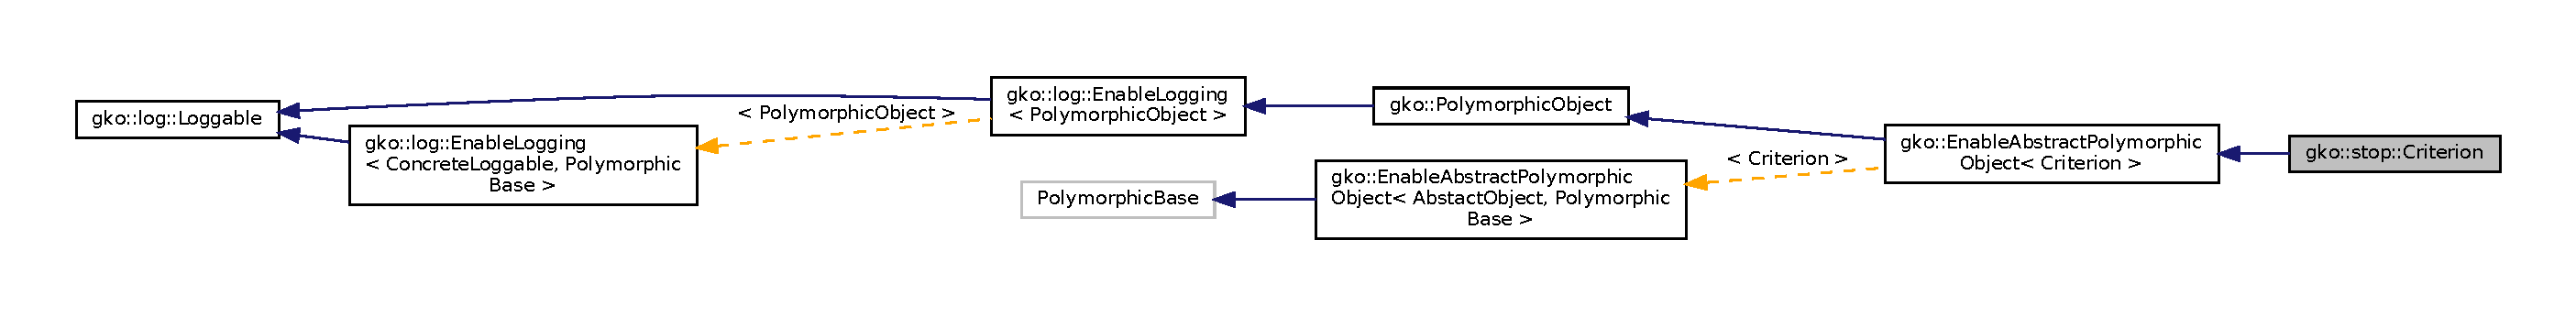
\includegraphics[width=350pt]{classgko_1_1stop_1_1Criterion__coll__graph}
\end{center}
\end{figure}
\subsection*{Classes}
\begin{DoxyCompactItemize}
\item 
class \hyperlink{classgko_1_1stop_1_1Criterion_1_1Updater}{Updater}
\begin{DoxyCompactList}\small\item\em The \hyperlink{classgko_1_1stop_1_1Criterion_1_1Updater}{Updater} class serves for convenient argument passing to the \hyperlink{classgko_1_1stop_1_1Criterion}{Criterion}\textquotesingle{}s check function. \end{DoxyCompactList}\end{DoxyCompactItemize}
\subsection*{Public Member Functions}
\begin{DoxyCompactItemize}
\item 
\hyperlink{classgko_1_1stop_1_1Criterion_1_1Updater}{Updater} \hyperlink{classgko_1_1stop_1_1Criterion_a47e22c46eaa742d709dcbf0d26d93e6c}{update} ()
\begin{DoxyCompactList}\small\item\em Returns the updater object. \end{DoxyCompactList}\item 
bool \hyperlink{classgko_1_1stop_1_1Criterion_a64634d8f02b439e5d8e6125fb996600d}{check} (\hyperlink{namespacegko_a3950fc3732811a8563484e5098c31531}{uint8} stopping\+Id, bool set\+Finalized, \hyperlink{classgko_1_1Array}{Array}$<$ \hyperlink{classgko_1_1stopping__status}{stopping\+\_\+status} $>$ $\ast$stop\+\_\+status, bool $\ast$one\+\_\+changed, const \hyperlink{classgko_1_1stop_1_1Criterion_1_1Updater}{Updater} \&updater)
\begin{DoxyCompactList}\small\item\em This checks whether convergence was reached for a certain criterion. \end{DoxyCompactList}\end{DoxyCompactItemize}


\subsection{Detailed Description}
The \hyperlink{classgko_1_1stop_1_1Criterion}{Criterion} class is a base class for all stopping criteria. 

It contains a factory to instantiate criteria. It is up to each specific stopping criterion to decide what to do with the data that is passed to it.

Note that depending on the criterion, convergence may not have happened after stopping. 

\subsection{Member Function Documentation}
\mbox{\Hypertarget{classgko_1_1stop_1_1Criterion_a64634d8f02b439e5d8e6125fb996600d}\label{classgko_1_1stop_1_1Criterion_a64634d8f02b439e5d8e6125fb996600d}} 
\index{gko\+::stop\+::\+Criterion@{gko\+::stop\+::\+Criterion}!check@{check}}
\index{check@{check}!gko\+::stop\+::\+Criterion@{gko\+::stop\+::\+Criterion}}
\subsubsection{\texorpdfstring{check()}{check()}}
{\footnotesize\ttfamily bool gko\+::stop\+::\+Criterion\+::check (\begin{DoxyParamCaption}\item[{\hyperlink{namespacegko_a3950fc3732811a8563484e5098c31531}{uint8}}]{stopping\+Id,  }\item[{bool}]{set\+Finalized,  }\item[{\hyperlink{classgko_1_1Array}{Array}$<$ \hyperlink{classgko_1_1stopping__status}{stopping\+\_\+status} $>$ $\ast$}]{stop\+\_\+status,  }\item[{bool $\ast$}]{one\+\_\+changed,  }\item[{const \hyperlink{classgko_1_1stop_1_1Criterion_1_1Updater}{Updater} \&}]{updater }\end{DoxyParamCaption})\hspace{0.3cm}{\ttfamily [inline]}}



This checks whether convergence was reached for a certain criterion. 

The actual implantation of the criterion goes here.


\begin{DoxyParams}{Parameters}
{\em stopping\+Id} & id of the stopping criterion \\
\hline
{\em set\+Finalized} & Controls if the current version should count as finalized or not \\
\hline
{\em stop\+\_\+status} & status of the stopping criterion \\
\hline
{\em one\+\_\+changed} & indicates if one vector\textquotesingle{}s status changed \\
\hline
{\em updater} & the \hyperlink{classgko_1_1stop_1_1Criterion_1_1Updater}{Updater} object containing all the information\\
\hline
\end{DoxyParams}
\begin{DoxyReturn}{Returns}
whether convergence was completely reached 
\end{DoxyReturn}


Referenced by gko\+::stop\+::\+Criterion\+::\+Updater\+::check().

\mbox{\Hypertarget{classgko_1_1stop_1_1Criterion_a47e22c46eaa742d709dcbf0d26d93e6c}\label{classgko_1_1stop_1_1Criterion_a47e22c46eaa742d709dcbf0d26d93e6c}} 
\index{gko\+::stop\+::\+Criterion@{gko\+::stop\+::\+Criterion}!update@{update}}
\index{update@{update}!gko\+::stop\+::\+Criterion@{gko\+::stop\+::\+Criterion}}
\subsubsection{\texorpdfstring{update()}{update()}}
{\footnotesize\ttfamily \hyperlink{classgko_1_1stop_1_1Criterion_1_1Updater}{Updater} gko\+::stop\+::\+Criterion\+::update (\begin{DoxyParamCaption}{ }\end{DoxyParamCaption})\hspace{0.3cm}{\ttfamily [inline]}}



Returns the updater object. 

\begin{DoxyReturn}{Returns}
the updater object 
\end{DoxyReturn}


The documentation for this class was generated from the following file\+:\begin{DoxyCompactItemize}
\item 
ginkgo/core/stop/criterion.\+hpp (f0a50f96)\end{DoxyCompactItemize}

\hypertarget{structgko_1_1log_1_1criterion__data}{}\doxysection{gko\+::log\+::criterion\+\_\+data Struct Reference}
\label{structgko_1_1log_1_1criterion__data}\index{gko::log::criterion\_data@{gko::log::criterion\_data}}


Struct representing Criterion related data.  




{\ttfamily \#include $<$ginkgo/core/log/record.\+hpp$>$}



Collaboration diagram for gko\+::log\+::criterion\+\_\+data\+:
\nopagebreak
\begin{figure}[H]
\begin{center}
\leavevmode
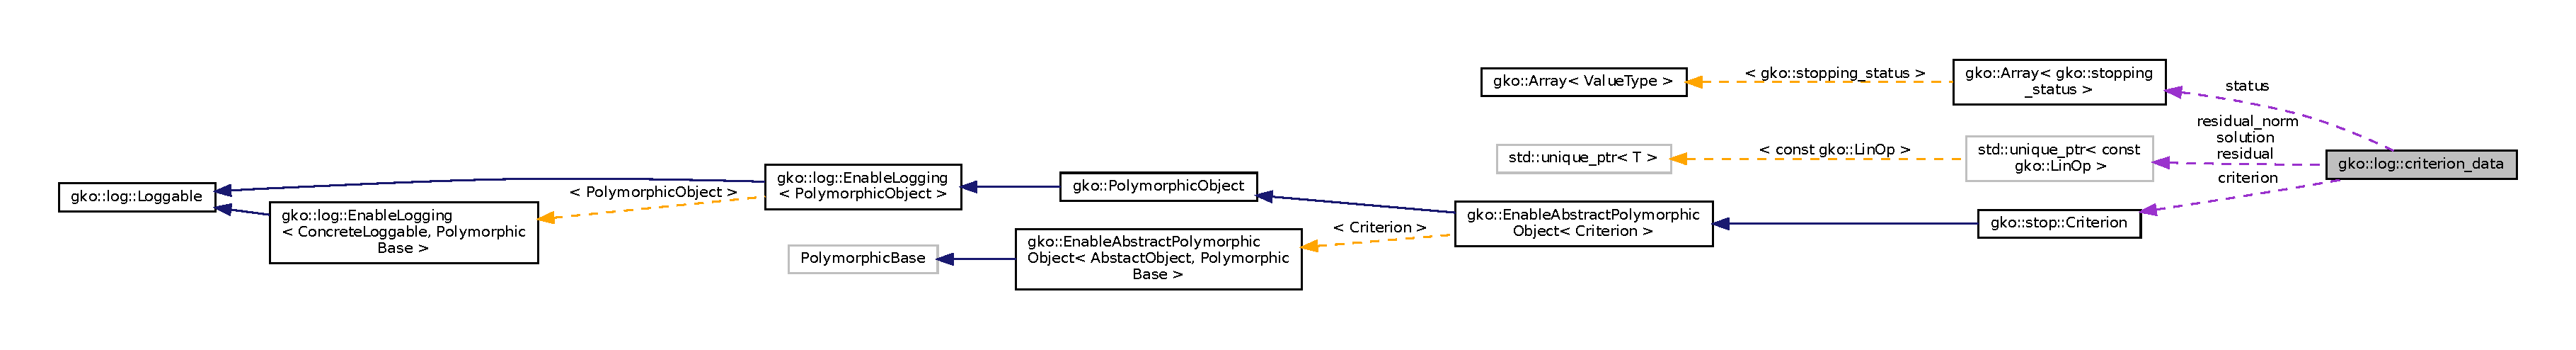
\includegraphics[width=350pt]{structgko_1_1log_1_1criterion__data__coll__graph}
\end{center}
\end{figure}
\doxysubsection*{Public Member Functions}
\begin{DoxyCompactItemize}
\item 
\mbox{\Hypertarget{structgko_1_1log_1_1criterion__data_a8643df5a8f5d0cb01f80823fbdc3f5a0}\label{structgko_1_1log_1_1criterion__data_a8643df5a8f5d0cb01f80823fbdc3f5a0}} 
{\bfseries criterion\+\_\+data} (const \mbox{\hyperlink{classgko_1_1stop_1_1Criterion}{stop\+::\+Criterion}} $\ast$criterion, const \mbox{\hyperlink{namespacegko_a6e5c95df0ae4e47aab2f604a22d98ee7}{size\+\_\+type}} \&num\+\_\+iterations, const \mbox{\hyperlink{classgko_1_1LinOp}{Lin\+Op}} $\ast$residual, const \mbox{\hyperlink{classgko_1_1LinOp}{Lin\+Op}} $\ast$residual\+\_\+norm, const \mbox{\hyperlink{classgko_1_1LinOp}{Lin\+Op}} $\ast$solution, const \mbox{\hyperlink{namespacegko_a3950fc3732811a8563484e5098c31531}{uint8}} stopping\+\_\+id, const bool set\+\_\+finalized, const \mbox{\hyperlink{classgko_1_1Array}{Array}}$<$ \mbox{\hyperlink{classgko_1_1stopping__status}{stopping\+\_\+status}} $>$ $\ast$status=nullptr, const bool one\+Changed=false, const bool converged=false)
\end{DoxyCompactItemize}
\doxysubsection*{Public Attributes}
\begin{DoxyCompactItemize}
\item 
\mbox{\Hypertarget{structgko_1_1log_1_1criterion__data_aa0548110c547da9a8483927718884f4a}\label{structgko_1_1log_1_1criterion__data_aa0548110c547da9a8483927718884f4a}} 
const \mbox{\hyperlink{classgko_1_1stop_1_1Criterion}{stop\+::\+Criterion}} $\ast$ {\bfseries criterion}
\item 
\mbox{\Hypertarget{structgko_1_1log_1_1criterion__data_afab8df7b4785439a9267bc652d6deb63}\label{structgko_1_1log_1_1criterion__data_afab8df7b4785439a9267bc652d6deb63}} 
const \mbox{\hyperlink{namespacegko_a6e5c95df0ae4e47aab2f604a22d98ee7}{size\+\_\+type}} {\bfseries num\+\_\+iterations}
\item 
\mbox{\Hypertarget{structgko_1_1log_1_1criterion__data_adc825d1d8a8e1c69e172ee582319a82a}\label{structgko_1_1log_1_1criterion__data_adc825d1d8a8e1c69e172ee582319a82a}} 
std\+::unique\+\_\+ptr$<$ const \mbox{\hyperlink{classgko_1_1LinOp}{Lin\+Op}} $>$ {\bfseries residual}
\item 
\mbox{\Hypertarget{structgko_1_1log_1_1criterion__data_a425258f5b1cb46ae3f117eace796a1f7}\label{structgko_1_1log_1_1criterion__data_a425258f5b1cb46ae3f117eace796a1f7}} 
std\+::unique\+\_\+ptr$<$ const \mbox{\hyperlink{classgko_1_1LinOp}{Lin\+Op}} $>$ {\bfseries residual\+\_\+norm}
\item 
\mbox{\Hypertarget{structgko_1_1log_1_1criterion__data_a23bddbadadb1ce48d21d41f8ac515d10}\label{structgko_1_1log_1_1criterion__data_a23bddbadadb1ce48d21d41f8ac515d10}} 
std\+::unique\+\_\+ptr$<$ const \mbox{\hyperlink{classgko_1_1LinOp}{Lin\+Op}} $>$ {\bfseries solution}
\item 
\mbox{\Hypertarget{structgko_1_1log_1_1criterion__data_ae406ca3e9f745e24edf545d33efdd7ce}\label{structgko_1_1log_1_1criterion__data_ae406ca3e9f745e24edf545d33efdd7ce}} 
const \mbox{\hyperlink{namespacegko_a3950fc3732811a8563484e5098c31531}{uint8}} {\bfseries stopping\+\_\+id}
\item 
\mbox{\Hypertarget{structgko_1_1log_1_1criterion__data_a4c807636a64d3b1078572aac0c0ce95f}\label{structgko_1_1log_1_1criterion__data_a4c807636a64d3b1078572aac0c0ce95f}} 
const bool {\bfseries set\+\_\+finalized}
\item 
\mbox{\Hypertarget{structgko_1_1log_1_1criterion__data_af795c317fb08a115e077fe30f27812c1}\label{structgko_1_1log_1_1criterion__data_af795c317fb08a115e077fe30f27812c1}} 
const \mbox{\hyperlink{classgko_1_1Array}{Array}}$<$ \mbox{\hyperlink{classgko_1_1stopping__status}{stopping\+\_\+status}} $>$ $\ast$ {\bfseries status}
\item 
\mbox{\Hypertarget{structgko_1_1log_1_1criterion__data_ac0008d49d33f2fa1f972fb98279bb162}\label{structgko_1_1log_1_1criterion__data_ac0008d49d33f2fa1f972fb98279bb162}} 
const bool {\bfseries one\+Changed}
\item 
\mbox{\Hypertarget{structgko_1_1log_1_1criterion__data_aa8fe52a61886be70613da84cfb3868f8}\label{structgko_1_1log_1_1criterion__data_aa8fe52a61886be70613da84cfb3868f8}} 
const bool {\bfseries converged}
\end{DoxyCompactItemize}


\doxysubsection{Detailed Description}
Struct representing Criterion related data. 

The documentation for this struct was generated from the following file\+:\begin{DoxyCompactItemize}
\item 
ginkgo/core/log/record.\+hpp (f0a50f96)\end{DoxyCompactItemize}

\hypertarget{structgko_1_1stop_1_1CriterionArgs}{}\doxysection{gko\+::stop\+::Criterion\+Args Struct Reference}
\label{structgko_1_1stop_1_1CriterionArgs}\index{gko::stop::CriterionArgs@{gko::stop::CriterionArgs}}


This struct is used to pass parameters to the Enable\+Default\+Criterion\+Factory\+Criterion\+Factory\+::generate() method.  




{\ttfamily \#include $<$ginkgo/core/stop/criterion.\+hpp$>$}



Collaboration diagram for gko\+::stop\+::Criterion\+Args\+:
\nopagebreak
\begin{figure}[H]
\begin{center}
\leavevmode
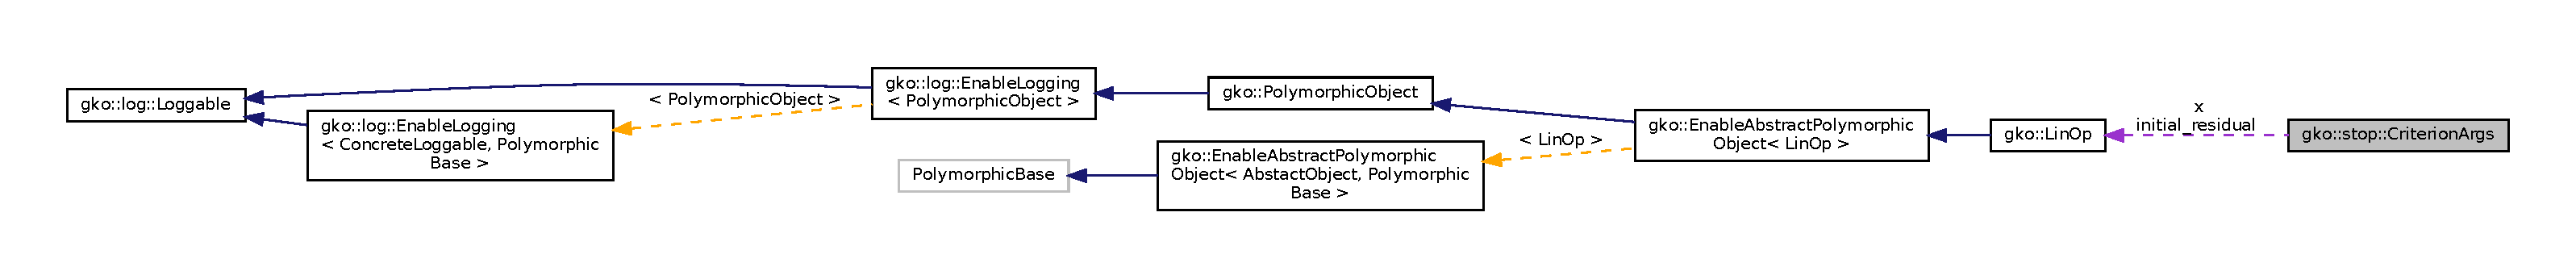
\includegraphics[width=350pt]{structgko_1_1stop_1_1CriterionArgs__coll__graph}
\end{center}
\end{figure}
\doxysubsection*{Public Member Functions}
\begin{DoxyCompactItemize}
\item 
\mbox{\Hypertarget{structgko_1_1stop_1_1CriterionArgs_aee534b8a229d17a5cca30e6fe2dcc05e}\label{structgko_1_1stop_1_1CriterionArgs_aee534b8a229d17a5cca30e6fe2dcc05e}} 
{\bfseries Criterion\+Args} (std\+::shared\+\_\+ptr$<$ const \mbox{\hyperlink{classgko_1_1LinOp}{Lin\+Op}} $>$ system\+\_\+matrix, std\+::shared\+\_\+ptr$<$ const \mbox{\hyperlink{classgko_1_1LinOp}{Lin\+Op}} $>$ b, const \mbox{\hyperlink{classgko_1_1LinOp}{Lin\+Op}} $\ast$x, const \mbox{\hyperlink{classgko_1_1LinOp}{Lin\+Op}} $\ast$initial\+\_\+residual=nullptr)
\end{DoxyCompactItemize}
\doxysubsection*{Public Attributes}
\begin{DoxyCompactItemize}
\item 
\mbox{\Hypertarget{structgko_1_1stop_1_1CriterionArgs_a2aa22bea76fd64352a446cf6c5570807}\label{structgko_1_1stop_1_1CriterionArgs_a2aa22bea76fd64352a446cf6c5570807}} 
std\+::shared\+\_\+ptr$<$ const \mbox{\hyperlink{classgko_1_1LinOp}{Lin\+Op}} $>$ {\bfseries system\+\_\+matrix}
\item 
\mbox{\Hypertarget{structgko_1_1stop_1_1CriterionArgs_a994457497657a0308c5343e711ec4c3e}\label{structgko_1_1stop_1_1CriterionArgs_a994457497657a0308c5343e711ec4c3e}} 
std\+::shared\+\_\+ptr$<$ const \mbox{\hyperlink{classgko_1_1LinOp}{Lin\+Op}} $>$ {\bfseries b}
\item 
\mbox{\Hypertarget{structgko_1_1stop_1_1CriterionArgs_a766a5c79ca77e74703888786e0011a73}\label{structgko_1_1stop_1_1CriterionArgs_a766a5c79ca77e74703888786e0011a73}} 
const \mbox{\hyperlink{classgko_1_1LinOp}{Lin\+Op}} $\ast$ {\bfseries x}
\item 
\mbox{\Hypertarget{structgko_1_1stop_1_1CriterionArgs_af7233105d01a9b055b15652daf179a67}\label{structgko_1_1stop_1_1CriterionArgs_af7233105d01a9b055b15652daf179a67}} 
const \mbox{\hyperlink{classgko_1_1LinOp}{Lin\+Op}} $\ast$ {\bfseries initial\+\_\+residual}
\end{DoxyCompactItemize}


\doxysubsection{Detailed Description}
This struct is used to pass parameters to the Enable\+Default\+Criterion\+Factory\+Criterion\+Factory\+::generate() method. 

It is the Components\+Type of Criterion\+Factory.

\begin{DoxyNote}{Note}
Dependly on the use case, some of these parameters can be {\ttfamily nullptr} as only some stopping criterion require them to be set. An example is the {\ttfamily \mbox{\hyperlink{classgko_1_1stop_1_1ResidualNormReduction}{Residual\+Norm\+Reduction}}} which really requires the {\ttfamily initial\+\_\+residual} to be set. 
\end{DoxyNote}


The documentation for this struct was generated from the following file\+:\begin{DoxyCompactItemize}
\item 
ginkgo/core/stop/criterion.\+hpp (da788090)\end{DoxyCompactItemize}

\hypertarget{classgko_1_1matrix_1_1Csr}{}\doxysection{gko\+::matrix\+::Csr$<$ Value\+Type, Index\+Type $>$ Class Template Reference}
\label{classgko_1_1matrix_1_1Csr}\index{gko::matrix::Csr$<$ ValueType, IndexType $>$@{gko::matrix::Csr$<$ ValueType, IndexType $>$}}


C\+SR is a matrix format which stores only the nonzero coefficients by compressing each row of the matrix (compressed sparse row format).  




{\ttfamily \#include $<$ginkgo/core/matrix/csr.\+hpp$>$}



Collaboration diagram for gko\+::matrix\+::Csr$<$ Value\+Type, Index\+Type $>$\+:
\nopagebreak
\begin{figure}[H]
\begin{center}
\leavevmode
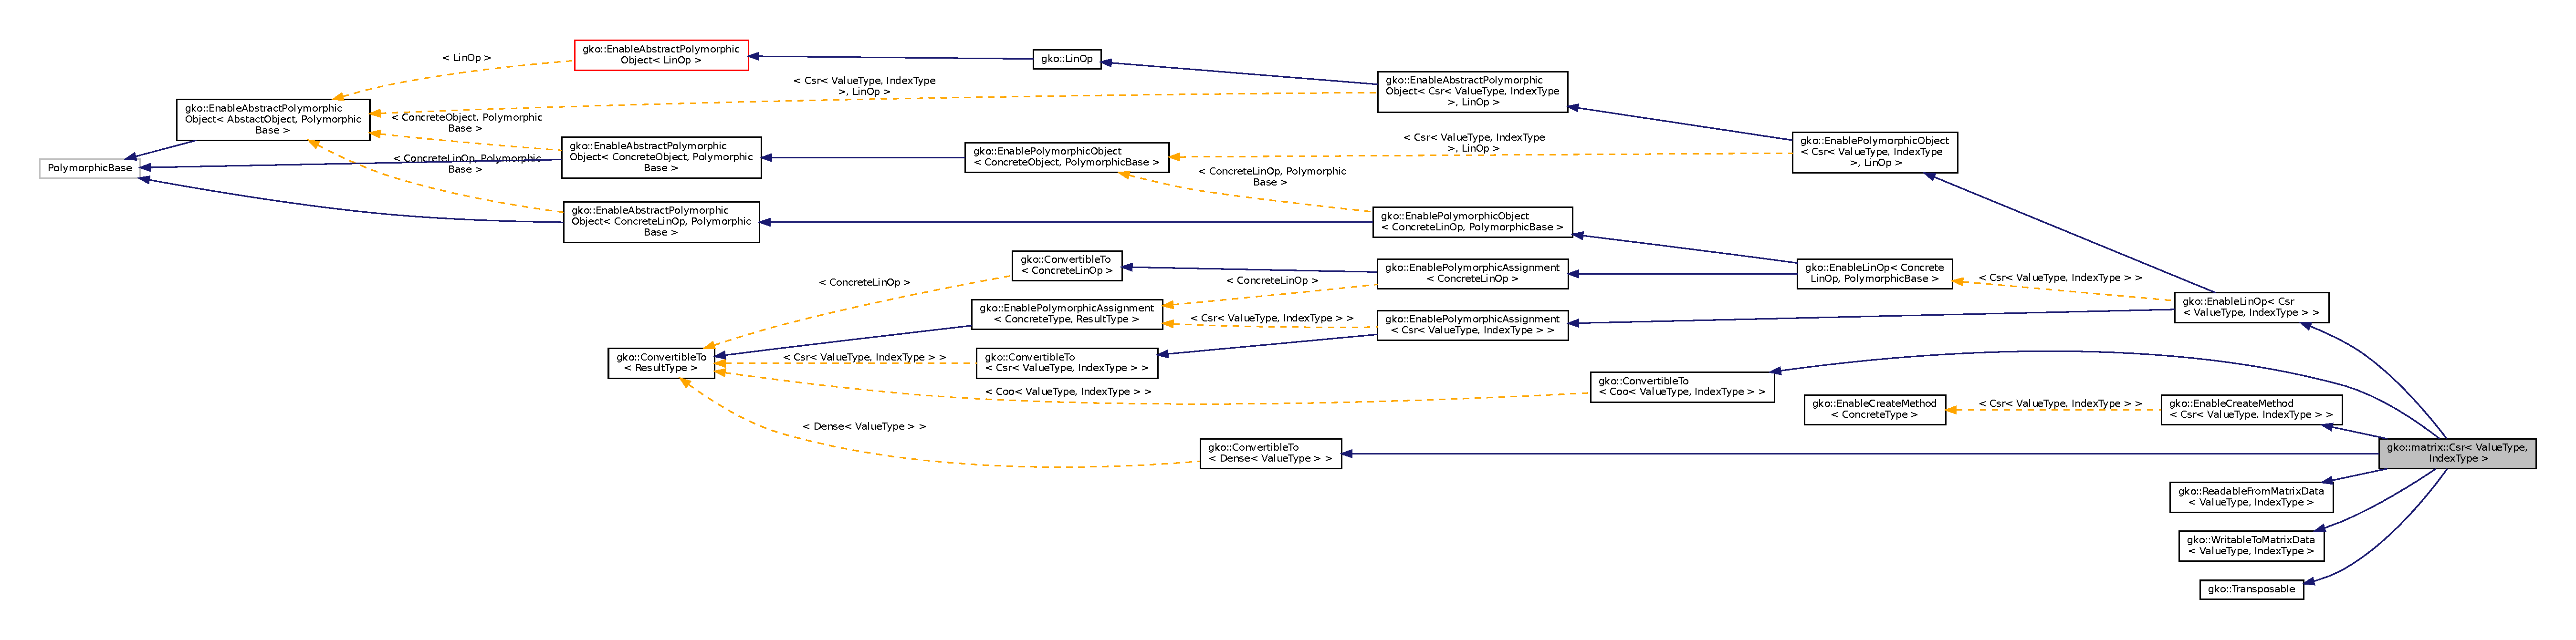
\includegraphics[width=350pt]{classgko_1_1matrix_1_1Csr__coll__graph}
\end{center}
\end{figure}
\doxysubsection*{Classes}
\begin{DoxyCompactItemize}
\item 
class \mbox{\hyperlink{classgko_1_1matrix_1_1Csr_1_1automatical}{automatical}}
\item 
class \mbox{\hyperlink{classgko_1_1matrix_1_1Csr_1_1classical}{classical}}
\item 
class \mbox{\hyperlink{classgko_1_1matrix_1_1Csr_1_1cusparse}{cusparse}}
\item 
class \mbox{\hyperlink{classgko_1_1matrix_1_1Csr_1_1load__balance}{load\+\_\+balance}}
\item 
class \mbox{\hyperlink{classgko_1_1matrix_1_1Csr_1_1merge__path}{merge\+\_\+path}}
\item 
class \mbox{\hyperlink{classgko_1_1matrix_1_1Csr_1_1strategy__type}{strategy\+\_\+type}}
\end{DoxyCompactItemize}
\doxysubsection*{Public Types}
\begin{DoxyCompactItemize}
\item 
\mbox{\Hypertarget{classgko_1_1matrix_1_1Csr_ae9e0b5332427a9a5a782aab4b6e2b60e}\label{classgko_1_1matrix_1_1Csr_ae9e0b5332427a9a5a782aab4b6e2b60e}} 
using {\bfseries value\+\_\+type} = Value\+Type
\item 
\mbox{\Hypertarget{classgko_1_1matrix_1_1Csr_a47f9c8f2945fc5d50e1eac99a9511174}\label{classgko_1_1matrix_1_1Csr_a47f9c8f2945fc5d50e1eac99a9511174}} 
using {\bfseries index\+\_\+type} = Index\+Type
\item 
\mbox{\Hypertarget{classgko_1_1matrix_1_1Csr_a4aeffed616fb42844161bd176f588785}\label{classgko_1_1matrix_1_1Csr_a4aeffed616fb42844161bd176f588785}} 
using {\bfseries mat\+\_\+data} = \mbox{\hyperlink{structgko_1_1matrix__data}{matrix\+\_\+data}}$<$ Value\+Type, Index\+Type $>$
\end{DoxyCompactItemize}
\doxysubsection*{Public Member Functions}
\begin{DoxyCompactItemize}
\item 
\mbox{\Hypertarget{classgko_1_1matrix_1_1Csr_a610dfb71907ee0e79ca6470571cb1d10}\label{classgko_1_1matrix_1_1Csr_a610dfb71907ee0e79ca6470571cb1d10}} 
void {\bfseries convert\+\_\+to} (\mbox{\hyperlink{classgko_1_1matrix_1_1Dense}{Dense}}$<$ Value\+Type $>$ $\ast$other) const override
\item 
\mbox{\Hypertarget{classgko_1_1matrix_1_1Csr_a794189da6f4443a991b7f68ed59c2f49}\label{classgko_1_1matrix_1_1Csr_a794189da6f4443a991b7f68ed59c2f49}} 
void {\bfseries move\+\_\+to} (\mbox{\hyperlink{classgko_1_1matrix_1_1Dense}{Dense}}$<$ Value\+Type $>$ $\ast$other) override
\item 
\mbox{\Hypertarget{classgko_1_1matrix_1_1Csr_ab0927bd9d5f77008d95891f266b9eb1d}\label{classgko_1_1matrix_1_1Csr_ab0927bd9d5f77008d95891f266b9eb1d}} 
void {\bfseries convert\+\_\+to} (\mbox{\hyperlink{classgko_1_1matrix_1_1Coo}{Coo}}$<$ Value\+Type, Index\+Type $>$ $\ast$result) const override
\item 
\mbox{\Hypertarget{classgko_1_1matrix_1_1Csr_a79c4a2730c1ef576d75fb8f2d98aecf2}\label{classgko_1_1matrix_1_1Csr_a79c4a2730c1ef576d75fb8f2d98aecf2}} 
void {\bfseries move\+\_\+to} (\mbox{\hyperlink{classgko_1_1matrix_1_1Coo}{Coo}}$<$ Value\+Type, Index\+Type $>$ $\ast$result) override
\item 
\mbox{\Hypertarget{classgko_1_1matrix_1_1Csr_a4c351ea53f42a6fd5792b38d786e2082}\label{classgko_1_1matrix_1_1Csr_a4c351ea53f42a6fd5792b38d786e2082}} 
void {\bfseries convert\+\_\+to} (\mbox{\hyperlink{classgko_1_1matrix_1_1Ell}{Ell}}$<$ Value\+Type, Index\+Type $>$ $\ast$result) const override
\item 
\mbox{\Hypertarget{classgko_1_1matrix_1_1Csr_a44c064ee29e926fe36c8298b7f435242}\label{classgko_1_1matrix_1_1Csr_a44c064ee29e926fe36c8298b7f435242}} 
void {\bfseries move\+\_\+to} (\mbox{\hyperlink{classgko_1_1matrix_1_1Ell}{Ell}}$<$ Value\+Type, Index\+Type $>$ $\ast$result) override
\item 
\mbox{\Hypertarget{classgko_1_1matrix_1_1Csr_a28bc89a11d683822fa1f0a20e1d54499}\label{classgko_1_1matrix_1_1Csr_a28bc89a11d683822fa1f0a20e1d54499}} 
void {\bfseries convert\+\_\+to} (\mbox{\hyperlink{classgko_1_1matrix_1_1Hybrid}{Hybrid}}$<$ Value\+Type, Index\+Type $>$ $\ast$result) const override
\item 
\mbox{\Hypertarget{classgko_1_1matrix_1_1Csr_a9c703e8d02140609f4a4c5b4a9f342ec}\label{classgko_1_1matrix_1_1Csr_a9c703e8d02140609f4a4c5b4a9f342ec}} 
void {\bfseries move\+\_\+to} (\mbox{\hyperlink{classgko_1_1matrix_1_1Hybrid}{Hybrid}}$<$ Value\+Type, Index\+Type $>$ $\ast$result) override
\item 
\mbox{\Hypertarget{classgko_1_1matrix_1_1Csr_aa7c16cb04e391ef7635e9b597ada39a3}\label{classgko_1_1matrix_1_1Csr_aa7c16cb04e391ef7635e9b597ada39a3}} 
void {\bfseries convert\+\_\+to} (\mbox{\hyperlink{classgko_1_1matrix_1_1Sellp}{Sellp}}$<$ Value\+Type, Index\+Type $>$ $\ast$result) const override
\item 
\mbox{\Hypertarget{classgko_1_1matrix_1_1Csr_ab5e533173f10bb8b0269ddf8374bfcff}\label{classgko_1_1matrix_1_1Csr_ab5e533173f10bb8b0269ddf8374bfcff}} 
void {\bfseries move\+\_\+to} (\mbox{\hyperlink{classgko_1_1matrix_1_1Sellp}{Sellp}}$<$ Value\+Type, Index\+Type $>$ $\ast$result) override
\item 
\mbox{\Hypertarget{classgko_1_1matrix_1_1Csr_aafef8f608dac1dbcee61f010cb612e23}\label{classgko_1_1matrix_1_1Csr_aafef8f608dac1dbcee61f010cb612e23}} 
void {\bfseries convert\+\_\+to} (\mbox{\hyperlink{classgko_1_1matrix_1_1SparsityCsr}{Sparsity\+Csr}}$<$ Value\+Type, Index\+Type $>$ $\ast$result) const override
\item 
\mbox{\Hypertarget{classgko_1_1matrix_1_1Csr_a5cc9ee296e55973438efed46468c9a55}\label{classgko_1_1matrix_1_1Csr_a5cc9ee296e55973438efed46468c9a55}} 
void {\bfseries move\+\_\+to} (\mbox{\hyperlink{classgko_1_1matrix_1_1SparsityCsr}{Sparsity\+Csr}}$<$ Value\+Type, Index\+Type $>$ $\ast$result) override
\item 
void \mbox{\hyperlink{classgko_1_1matrix_1_1Csr_ac4db41146ed3c3a8653b03d6b2c6c675}{read}} (const \mbox{\hyperlink{structgko_1_1matrix__data}{mat\+\_\+data}} \&data) override
\begin{DoxyCompactList}\small\item\em Reads a matrix from a \mbox{\hyperlink{structgko_1_1matrix__data}{matrix\+\_\+data}} structure. \end{DoxyCompactList}\item 
void \mbox{\hyperlink{classgko_1_1matrix_1_1Csr_a205fc391f4cf4f7718a55b0a61f62bc9}{write}} (\mbox{\hyperlink{structgko_1_1matrix__data}{mat\+\_\+data}} \&data) const override
\begin{DoxyCompactList}\small\item\em Writes a matrix to a \mbox{\hyperlink{structgko_1_1matrix__data}{matrix\+\_\+data}} structure. \end{DoxyCompactList}\item 
std\+::unique\+\_\+ptr$<$ \mbox{\hyperlink{classgko_1_1LinOp}{Lin\+Op}} $>$ \mbox{\hyperlink{classgko_1_1matrix_1_1Csr_ab79e609214d6b4834d5961ee0a7d3519}{transpose}} () const override
\begin{DoxyCompactList}\small\item\em Returns a \mbox{\hyperlink{classgko_1_1LinOp}{Lin\+Op}} representing the transpose of the \mbox{\hyperlink{classgko_1_1Transposable}{Transposable}} object. \end{DoxyCompactList}\item 
std\+::unique\+\_\+ptr$<$ \mbox{\hyperlink{classgko_1_1LinOp}{Lin\+Op}} $>$ \mbox{\hyperlink{classgko_1_1matrix_1_1Csr_a38820451af5424f18b767667f3067d72}{conj\+\_\+transpose}} () const override
\begin{DoxyCompactList}\small\item\em Returns a \mbox{\hyperlink{classgko_1_1LinOp}{Lin\+Op}} representing the conjugate transpose of the \mbox{\hyperlink{classgko_1_1Transposable}{Transposable}} object. \end{DoxyCompactList}\item 
\mbox{\Hypertarget{classgko_1_1matrix_1_1Csr_ac817665ebedfc099180a785d813db8ef}\label{classgko_1_1matrix_1_1Csr_ac817665ebedfc099180a785d813db8ef}} 
void \mbox{\hyperlink{classgko_1_1matrix_1_1Csr_ac817665ebedfc099180a785d813db8ef}{sort\+\_\+by\+\_\+column\+\_\+index}} ()
\begin{DoxyCompactList}\small\item\em Sorts all (value, col\+\_\+idx) pairs in each row by column index. \end{DoxyCompactList}\item 
\mbox{\Hypertarget{classgko_1_1matrix_1_1Csr_adf7499e248badc9faed07c84e3a2449c}\label{classgko_1_1matrix_1_1Csr_adf7499e248badc9faed07c84e3a2449c}} 
bool {\bfseries is\+\_\+sorted\+\_\+by\+\_\+column\+\_\+index} () const
\item 
value\+\_\+type $\ast$ \mbox{\hyperlink{classgko_1_1matrix_1_1Csr_a929b0a194e6aeb1252b8e6781d162e83}{get\+\_\+values}} () noexcept
\begin{DoxyCompactList}\small\item\em Returns the values of the matrix. \end{DoxyCompactList}\item 
const value\+\_\+type $\ast$ \mbox{\hyperlink{classgko_1_1matrix_1_1Csr_a1801347665214bbefc837b44ba0695ff}{get\+\_\+const\+\_\+values}} () const noexcept
\begin{DoxyCompactList}\small\item\em Returns the values of the matrix. \end{DoxyCompactList}\item 
index\+\_\+type $\ast$ \mbox{\hyperlink{classgko_1_1matrix_1_1Csr_a81c6294177a1be4873804c8a85a9fc64}{get\+\_\+col\+\_\+idxs}} () noexcept
\begin{DoxyCompactList}\small\item\em Returns the column indexes of the matrix. \end{DoxyCompactList}\item 
const index\+\_\+type $\ast$ \mbox{\hyperlink{classgko_1_1matrix_1_1Csr_ac9d640d26449e0ee46c7cb2b80100d65}{get\+\_\+const\+\_\+col\+\_\+idxs}} () const noexcept
\begin{DoxyCompactList}\small\item\em Returns the column indexes of the matrix. \end{DoxyCompactList}\item 
index\+\_\+type $\ast$ \mbox{\hyperlink{classgko_1_1matrix_1_1Csr_a068e5158cf282fa977f0a137f8cd7f03}{get\+\_\+row\+\_\+ptrs}} () noexcept
\begin{DoxyCompactList}\small\item\em Returns the row pointers of the matrix. \end{DoxyCompactList}\item 
const index\+\_\+type $\ast$ \mbox{\hyperlink{classgko_1_1matrix_1_1Csr_a50c9ce521649450d7ae5ff488e42c190}{get\+\_\+const\+\_\+row\+\_\+ptrs}} () const noexcept
\begin{DoxyCompactList}\small\item\em Returns the row pointers of the matrix. \end{DoxyCompactList}\item 
index\+\_\+type $\ast$ \mbox{\hyperlink{classgko_1_1matrix_1_1Csr_a919fb1efdcbde6fba7eb18bdc39ba46a}{get\+\_\+srow}} () noexcept
\begin{DoxyCompactList}\small\item\em Returns the starting rows. \end{DoxyCompactList}\item 
const index\+\_\+type $\ast$ \mbox{\hyperlink{classgko_1_1matrix_1_1Csr_ac046f27c47848bf31c9234567661ef48}{get\+\_\+const\+\_\+srow}} () const noexcept
\begin{DoxyCompactList}\small\item\em Returns the starting rows. \end{DoxyCompactList}\item 
\mbox{\hyperlink{namespacegko_a6e5c95df0ae4e47aab2f604a22d98ee7}{size\+\_\+type}} \mbox{\hyperlink{classgko_1_1matrix_1_1Csr_a5b8c25c2fb1bbea62a3afdec8f8340c5}{get\+\_\+num\+\_\+srow\+\_\+elements}} () const noexcept
\begin{DoxyCompactList}\small\item\em Returns the number of the srow stored elements (involved warps) \end{DoxyCompactList}\item 
\mbox{\hyperlink{namespacegko_a6e5c95df0ae4e47aab2f604a22d98ee7}{size\+\_\+type}} \mbox{\hyperlink{classgko_1_1matrix_1_1Csr_ab70c085fc3df11a4ed9fe74b40844c5c}{get\+\_\+num\+\_\+stored\+\_\+elements}} () const noexcept
\begin{DoxyCompactList}\small\item\em Returns the number of elements explicitly stored in the matrix. \end{DoxyCompactList}\item 
std\+::shared\+\_\+ptr$<$ \mbox{\hyperlink{classgko_1_1matrix_1_1Csr_1_1strategy__type}{strategy\+\_\+type}} $>$ \mbox{\hyperlink{classgko_1_1matrix_1_1Csr_ada0db14e65dfe027f483dc449f704a7e}{get\+\_\+strategy}} () const noexcept
\begin{DoxyCompactList}\small\item\em Returns the strategy. \end{DoxyCompactList}\end{DoxyCompactItemize}
\doxysubsection*{Friends}
\begin{DoxyCompactItemize}
\item 
\mbox{\Hypertarget{classgko_1_1matrix_1_1Csr_ad8cd96663ce0ef68ea6d54f3d163df35}\label{classgko_1_1matrix_1_1Csr_ad8cd96663ce0ef68ea6d54f3d163df35}} 
class {\bfseries Enable\+Create\+Method$<$ Csr $>$}
\item 
\mbox{\Hypertarget{classgko_1_1matrix_1_1Csr_a6fa2ee2c326608dac42afed82be6713c}\label{classgko_1_1matrix_1_1Csr_a6fa2ee2c326608dac42afed82be6713c}} 
class {\bfseries Enable\+Polymorphic\+Object$<$ Csr, Lin\+Op $>$}
\item 
\mbox{\Hypertarget{classgko_1_1matrix_1_1Csr_ad2572ffab980b4728254b155909b3119}\label{classgko_1_1matrix_1_1Csr_ad2572ffab980b4728254b155909b3119}} 
class {\bfseries Coo$<$ Value\+Type, Index\+Type $>$}
\item 
\mbox{\Hypertarget{classgko_1_1matrix_1_1Csr_a22a84c8f67f946aa60a2fa8bf5835a32}\label{classgko_1_1matrix_1_1Csr_a22a84c8f67f946aa60a2fa8bf5835a32}} 
class {\bfseries Dense$<$ Value\+Type $>$}
\item 
\mbox{\Hypertarget{classgko_1_1matrix_1_1Csr_aed957ed9db4269e50fc8aa3d0263e618}\label{classgko_1_1matrix_1_1Csr_aed957ed9db4269e50fc8aa3d0263e618}} 
class {\bfseries Ell$<$ Value\+Type, Index\+Type $>$}
\item 
\mbox{\Hypertarget{classgko_1_1matrix_1_1Csr_a86254b0ae570c27f5ba169d64b74e94b}\label{classgko_1_1matrix_1_1Csr_a86254b0ae570c27f5ba169d64b74e94b}} 
class {\bfseries Hybrid$<$ Value\+Type, Index\+Type $>$}
\item 
\mbox{\Hypertarget{classgko_1_1matrix_1_1Csr_a400cb6dae6e6294b9f7d0249d63d538c}\label{classgko_1_1matrix_1_1Csr_a400cb6dae6e6294b9f7d0249d63d538c}} 
class {\bfseries Sellp$<$ Value\+Type, Index\+Type $>$}
\item 
\mbox{\Hypertarget{classgko_1_1matrix_1_1Csr_af3670b1e6b4be191b76955732bbc46c1}\label{classgko_1_1matrix_1_1Csr_af3670b1e6b4be191b76955732bbc46c1}} 
class {\bfseries Sparsity\+Csr$<$ Value\+Type, Index\+Type $>$}
\end{DoxyCompactItemize}
\doxysubsection*{Additional Inherited Members}


\doxysubsection{Detailed Description}
\subsubsection*{template$<$typename Value\+Type = default\+\_\+precision, typename Index\+Type = int32$>$\newline
class gko\+::matrix\+::\+Csr$<$ Value\+Type, Index\+Type $>$}

C\+SR is a matrix format which stores only the nonzero coefficients by compressing each row of the matrix (compressed sparse row format). 

The nonzero elements are stored in a 1D array row-\/wise, and accompanied with a row pointer array which stores the starting index of each row. An additional column index array is used to identify the column of each nonzero element.


\begin{DoxyTemplParams}{Template Parameters}
{\em Value\+Type} & precision of matrix elements \\
\hline
{\em Index\+Type} & precision of matrix indexes \\
\hline
\end{DoxyTemplParams}


\doxysubsection{Member Function Documentation}
\mbox{\Hypertarget{classgko_1_1matrix_1_1Csr_a38820451af5424f18b767667f3067d72}\label{classgko_1_1matrix_1_1Csr_a38820451af5424f18b767667f3067d72}} 
\index{gko::matrix::Csr$<$ ValueType, IndexType $>$@{gko::matrix::Csr$<$ ValueType, IndexType $>$}!conj\_transpose@{conj\_transpose}}
\index{conj\_transpose@{conj\_transpose}!gko::matrix::Csr$<$ ValueType, IndexType $>$@{gko::matrix::Csr$<$ ValueType, IndexType $>$}}
\doxysubsubsection{\texorpdfstring{conj\_transpose()}{conj\_transpose()}}
{\footnotesize\ttfamily template$<$typename Value\+Type = default\+\_\+precision, typename Index\+Type = int32$>$ \\
std\+::unique\+\_\+ptr$<$\mbox{\hyperlink{classgko_1_1LinOp}{Lin\+Op}}$>$ \mbox{\hyperlink{classgko_1_1matrix_1_1Csr}{gko\+::matrix\+::\+Csr}}$<$ Value\+Type, Index\+Type $>$\+::conj\+\_\+transpose (\begin{DoxyParamCaption}{ }\end{DoxyParamCaption}) const\hspace{0.3cm}{\ttfamily [override]}, {\ttfamily [virtual]}}



Returns a \mbox{\hyperlink{classgko_1_1LinOp}{Lin\+Op}} representing the conjugate transpose of the \mbox{\hyperlink{classgko_1_1Transposable}{Transposable}} object. 

\begin{DoxyReturn}{Returns}
a pointer to the new conjugate transposed object 
\end{DoxyReturn}


Implements \mbox{\hyperlink{classgko_1_1Transposable_ab41b669288740cf2a6f7bf76e875b077}{gko\+::\+Transposable}}.

\mbox{\Hypertarget{classgko_1_1matrix_1_1Csr_a81c6294177a1be4873804c8a85a9fc64}\label{classgko_1_1matrix_1_1Csr_a81c6294177a1be4873804c8a85a9fc64}} 
\index{gko::matrix::Csr$<$ ValueType, IndexType $>$@{gko::matrix::Csr$<$ ValueType, IndexType $>$}!get\_col\_idxs@{get\_col\_idxs}}
\index{get\_col\_idxs@{get\_col\_idxs}!gko::matrix::Csr$<$ ValueType, IndexType $>$@{gko::matrix::Csr$<$ ValueType, IndexType $>$}}
\doxysubsubsection{\texorpdfstring{get\_col\_idxs()}{get\_col\_idxs()}}
{\footnotesize\ttfamily template$<$typename Value\+Type = default\+\_\+precision, typename Index\+Type = int32$>$ \\
index\+\_\+type$\ast$ \mbox{\hyperlink{classgko_1_1matrix_1_1Csr}{gko\+::matrix\+::\+Csr}}$<$ Value\+Type, Index\+Type $>$\+::get\+\_\+col\+\_\+idxs (\begin{DoxyParamCaption}{ }\end{DoxyParamCaption})\hspace{0.3cm}{\ttfamily [inline]}, {\ttfamily [noexcept]}}



Returns the column indexes of the matrix. 

\begin{DoxyReturn}{Returns}
the column indexes of the matrix. 
\end{DoxyReturn}


References gko\+::\+Array$<$ Value\+Type $>$\+::get\+\_\+data().

\mbox{\Hypertarget{classgko_1_1matrix_1_1Csr_ac9d640d26449e0ee46c7cb2b80100d65}\label{classgko_1_1matrix_1_1Csr_ac9d640d26449e0ee46c7cb2b80100d65}} 
\index{gko::matrix::Csr$<$ ValueType, IndexType $>$@{gko::matrix::Csr$<$ ValueType, IndexType $>$}!get\_const\_col\_idxs@{get\_const\_col\_idxs}}
\index{get\_const\_col\_idxs@{get\_const\_col\_idxs}!gko::matrix::Csr$<$ ValueType, IndexType $>$@{gko::matrix::Csr$<$ ValueType, IndexType $>$}}
\doxysubsubsection{\texorpdfstring{get\_const\_col\_idxs()}{get\_const\_col\_idxs()}}
{\footnotesize\ttfamily template$<$typename Value\+Type = default\+\_\+precision, typename Index\+Type = int32$>$ \\
const index\+\_\+type$\ast$ \mbox{\hyperlink{classgko_1_1matrix_1_1Csr}{gko\+::matrix\+::\+Csr}}$<$ Value\+Type, Index\+Type $>$\+::get\+\_\+const\+\_\+col\+\_\+idxs (\begin{DoxyParamCaption}{ }\end{DoxyParamCaption}) const\hspace{0.3cm}{\ttfamily [inline]}, {\ttfamily [noexcept]}}



Returns the column indexes of the matrix. 

\begin{DoxyReturn}{Returns}
the column indexes of the matrix.
\end{DoxyReturn}
\begin{DoxyNote}{Note}
This is the constant version of the function, which can be significantly more memory efficient than the non-\/constant version, so always prefer this version. 
\end{DoxyNote}


References gko\+::\+Array$<$ Value\+Type $>$\+::get\+\_\+const\+\_\+data().

\mbox{\Hypertarget{classgko_1_1matrix_1_1Csr_a50c9ce521649450d7ae5ff488e42c190}\label{classgko_1_1matrix_1_1Csr_a50c9ce521649450d7ae5ff488e42c190}} 
\index{gko::matrix::Csr$<$ ValueType, IndexType $>$@{gko::matrix::Csr$<$ ValueType, IndexType $>$}!get\_const\_row\_ptrs@{get\_const\_row\_ptrs}}
\index{get\_const\_row\_ptrs@{get\_const\_row\_ptrs}!gko::matrix::Csr$<$ ValueType, IndexType $>$@{gko::matrix::Csr$<$ ValueType, IndexType $>$}}
\doxysubsubsection{\texorpdfstring{get\_const\_row\_ptrs()}{get\_const\_row\_ptrs()}}
{\footnotesize\ttfamily template$<$typename Value\+Type = default\+\_\+precision, typename Index\+Type = int32$>$ \\
const index\+\_\+type$\ast$ \mbox{\hyperlink{classgko_1_1matrix_1_1Csr}{gko\+::matrix\+::\+Csr}}$<$ Value\+Type, Index\+Type $>$\+::get\+\_\+const\+\_\+row\+\_\+ptrs (\begin{DoxyParamCaption}{ }\end{DoxyParamCaption}) const\hspace{0.3cm}{\ttfamily [inline]}, {\ttfamily [noexcept]}}



Returns the row pointers of the matrix. 

\begin{DoxyReturn}{Returns}
the row pointers of the matrix.
\end{DoxyReturn}
\begin{DoxyNote}{Note}
This is the constant version of the function, which can be significantly more memory efficient than the non-\/constant version, so always prefer this version. 
\end{DoxyNote}


References gko\+::\+Array$<$ Value\+Type $>$\+::get\+\_\+const\+\_\+data().

\mbox{\Hypertarget{classgko_1_1matrix_1_1Csr_ac046f27c47848bf31c9234567661ef48}\label{classgko_1_1matrix_1_1Csr_ac046f27c47848bf31c9234567661ef48}} 
\index{gko::matrix::Csr$<$ ValueType, IndexType $>$@{gko::matrix::Csr$<$ ValueType, IndexType $>$}!get\_const\_srow@{get\_const\_srow}}
\index{get\_const\_srow@{get\_const\_srow}!gko::matrix::Csr$<$ ValueType, IndexType $>$@{gko::matrix::Csr$<$ ValueType, IndexType $>$}}
\doxysubsubsection{\texorpdfstring{get\_const\_srow()}{get\_const\_srow()}}
{\footnotesize\ttfamily template$<$typename Value\+Type = default\+\_\+precision, typename Index\+Type = int32$>$ \\
const index\+\_\+type$\ast$ \mbox{\hyperlink{classgko_1_1matrix_1_1Csr}{gko\+::matrix\+::\+Csr}}$<$ Value\+Type, Index\+Type $>$\+::get\+\_\+const\+\_\+srow (\begin{DoxyParamCaption}{ }\end{DoxyParamCaption}) const\hspace{0.3cm}{\ttfamily [inline]}, {\ttfamily [noexcept]}}



Returns the starting rows. 

\begin{DoxyReturn}{Returns}
the starting rows.
\end{DoxyReturn}
\begin{DoxyNote}{Note}
This is the constant version of the function, which can be significantly more memory efficient than the non-\/constant version, so always prefer this version. 
\end{DoxyNote}


References gko\+::\+Array$<$ Value\+Type $>$\+::get\+\_\+const\+\_\+data().

\mbox{\Hypertarget{classgko_1_1matrix_1_1Csr_a1801347665214bbefc837b44ba0695ff}\label{classgko_1_1matrix_1_1Csr_a1801347665214bbefc837b44ba0695ff}} 
\index{gko::matrix::Csr$<$ ValueType, IndexType $>$@{gko::matrix::Csr$<$ ValueType, IndexType $>$}!get\_const\_values@{get\_const\_values}}
\index{get\_const\_values@{get\_const\_values}!gko::matrix::Csr$<$ ValueType, IndexType $>$@{gko::matrix::Csr$<$ ValueType, IndexType $>$}}
\doxysubsubsection{\texorpdfstring{get\_const\_values()}{get\_const\_values()}}
{\footnotesize\ttfamily template$<$typename Value\+Type = default\+\_\+precision, typename Index\+Type = int32$>$ \\
const value\+\_\+type$\ast$ \mbox{\hyperlink{classgko_1_1matrix_1_1Csr}{gko\+::matrix\+::\+Csr}}$<$ Value\+Type, Index\+Type $>$\+::get\+\_\+const\+\_\+values (\begin{DoxyParamCaption}{ }\end{DoxyParamCaption}) const\hspace{0.3cm}{\ttfamily [inline]}, {\ttfamily [noexcept]}}



Returns the values of the matrix. 

\begin{DoxyReturn}{Returns}
the values of the matrix.
\end{DoxyReturn}
\begin{DoxyNote}{Note}
This is the constant version of the function, which can be significantly more memory efficient than the non-\/constant version, so always prefer this version. 
\end{DoxyNote}


References gko\+::\+Array$<$ Value\+Type $>$\+::get\+\_\+const\+\_\+data().

\mbox{\Hypertarget{classgko_1_1matrix_1_1Csr_a5b8c25c2fb1bbea62a3afdec8f8340c5}\label{classgko_1_1matrix_1_1Csr_a5b8c25c2fb1bbea62a3afdec8f8340c5}} 
\index{gko::matrix::Csr$<$ ValueType, IndexType $>$@{gko::matrix::Csr$<$ ValueType, IndexType $>$}!get\_num\_srow\_elements@{get\_num\_srow\_elements}}
\index{get\_num\_srow\_elements@{get\_num\_srow\_elements}!gko::matrix::Csr$<$ ValueType, IndexType $>$@{gko::matrix::Csr$<$ ValueType, IndexType $>$}}
\doxysubsubsection{\texorpdfstring{get\_num\_srow\_elements()}{get\_num\_srow\_elements()}}
{\footnotesize\ttfamily template$<$typename Value\+Type = default\+\_\+precision, typename Index\+Type = int32$>$ \\
\mbox{\hyperlink{namespacegko_a6e5c95df0ae4e47aab2f604a22d98ee7}{size\+\_\+type}} \mbox{\hyperlink{classgko_1_1matrix_1_1Csr}{gko\+::matrix\+::\+Csr}}$<$ Value\+Type, Index\+Type $>$\+::get\+\_\+num\+\_\+srow\+\_\+elements (\begin{DoxyParamCaption}{ }\end{DoxyParamCaption}) const\hspace{0.3cm}{\ttfamily [inline]}, {\ttfamily [noexcept]}}



Returns the number of the srow stored elements (involved warps) 

\begin{DoxyReturn}{Returns}
the number of the srow stored elements (involved warps) 
\end{DoxyReturn}


References gko\+::\+Array$<$ Value\+Type $>$\+::get\+\_\+num\+\_\+elems().

\mbox{\Hypertarget{classgko_1_1matrix_1_1Csr_ab70c085fc3df11a4ed9fe74b40844c5c}\label{classgko_1_1matrix_1_1Csr_ab70c085fc3df11a4ed9fe74b40844c5c}} 
\index{gko::matrix::Csr$<$ ValueType, IndexType $>$@{gko::matrix::Csr$<$ ValueType, IndexType $>$}!get\_num\_stored\_elements@{get\_num\_stored\_elements}}
\index{get\_num\_stored\_elements@{get\_num\_stored\_elements}!gko::matrix::Csr$<$ ValueType, IndexType $>$@{gko::matrix::Csr$<$ ValueType, IndexType $>$}}
\doxysubsubsection{\texorpdfstring{get\_num\_stored\_elements()}{get\_num\_stored\_elements()}}
{\footnotesize\ttfamily template$<$typename Value\+Type = default\+\_\+precision, typename Index\+Type = int32$>$ \\
\mbox{\hyperlink{namespacegko_a6e5c95df0ae4e47aab2f604a22d98ee7}{size\+\_\+type}} \mbox{\hyperlink{classgko_1_1matrix_1_1Csr}{gko\+::matrix\+::\+Csr}}$<$ Value\+Type, Index\+Type $>$\+::get\+\_\+num\+\_\+stored\+\_\+elements (\begin{DoxyParamCaption}{ }\end{DoxyParamCaption}) const\hspace{0.3cm}{\ttfamily [inline]}, {\ttfamily [noexcept]}}



Returns the number of elements explicitly stored in the matrix. 

\begin{DoxyReturn}{Returns}
the number of elements explicitly stored in the matrix 
\end{DoxyReturn}


References gko\+::\+Array$<$ Value\+Type $>$\+::get\+\_\+num\+\_\+elems().

\mbox{\Hypertarget{classgko_1_1matrix_1_1Csr_a068e5158cf282fa977f0a137f8cd7f03}\label{classgko_1_1matrix_1_1Csr_a068e5158cf282fa977f0a137f8cd7f03}} 
\index{gko::matrix::Csr$<$ ValueType, IndexType $>$@{gko::matrix::Csr$<$ ValueType, IndexType $>$}!get\_row\_ptrs@{get\_row\_ptrs}}
\index{get\_row\_ptrs@{get\_row\_ptrs}!gko::matrix::Csr$<$ ValueType, IndexType $>$@{gko::matrix::Csr$<$ ValueType, IndexType $>$}}
\doxysubsubsection{\texorpdfstring{get\_row\_ptrs()}{get\_row\_ptrs()}}
{\footnotesize\ttfamily template$<$typename Value\+Type = default\+\_\+precision, typename Index\+Type = int32$>$ \\
index\+\_\+type$\ast$ \mbox{\hyperlink{classgko_1_1matrix_1_1Csr}{gko\+::matrix\+::\+Csr}}$<$ Value\+Type, Index\+Type $>$\+::get\+\_\+row\+\_\+ptrs (\begin{DoxyParamCaption}{ }\end{DoxyParamCaption})\hspace{0.3cm}{\ttfamily [inline]}, {\ttfamily [noexcept]}}



Returns the row pointers of the matrix. 

\begin{DoxyReturn}{Returns}
the row pointers of the matrix. 
\end{DoxyReturn}


References gko\+::\+Array$<$ Value\+Type $>$\+::get\+\_\+data().

\mbox{\Hypertarget{classgko_1_1matrix_1_1Csr_a919fb1efdcbde6fba7eb18bdc39ba46a}\label{classgko_1_1matrix_1_1Csr_a919fb1efdcbde6fba7eb18bdc39ba46a}} 
\index{gko::matrix::Csr$<$ ValueType, IndexType $>$@{gko::matrix::Csr$<$ ValueType, IndexType $>$}!get\_srow@{get\_srow}}
\index{get\_srow@{get\_srow}!gko::matrix::Csr$<$ ValueType, IndexType $>$@{gko::matrix::Csr$<$ ValueType, IndexType $>$}}
\doxysubsubsection{\texorpdfstring{get\_srow()}{get\_srow()}}
{\footnotesize\ttfamily template$<$typename Value\+Type = default\+\_\+precision, typename Index\+Type = int32$>$ \\
index\+\_\+type$\ast$ \mbox{\hyperlink{classgko_1_1matrix_1_1Csr}{gko\+::matrix\+::\+Csr}}$<$ Value\+Type, Index\+Type $>$\+::get\+\_\+srow (\begin{DoxyParamCaption}{ }\end{DoxyParamCaption})\hspace{0.3cm}{\ttfamily [inline]}, {\ttfamily [noexcept]}}



Returns the starting rows. 

\begin{DoxyReturn}{Returns}
the starting rows. 
\end{DoxyReturn}


References gko\+::\+Array$<$ Value\+Type $>$\+::get\+\_\+data().

\mbox{\Hypertarget{classgko_1_1matrix_1_1Csr_ada0db14e65dfe027f483dc449f704a7e}\label{classgko_1_1matrix_1_1Csr_ada0db14e65dfe027f483dc449f704a7e}} 
\index{gko::matrix::Csr$<$ ValueType, IndexType $>$@{gko::matrix::Csr$<$ ValueType, IndexType $>$}!get\_strategy@{get\_strategy}}
\index{get\_strategy@{get\_strategy}!gko::matrix::Csr$<$ ValueType, IndexType $>$@{gko::matrix::Csr$<$ ValueType, IndexType $>$}}
\doxysubsubsection{\texorpdfstring{get\_strategy()}{get\_strategy()}}
{\footnotesize\ttfamily template$<$typename Value\+Type = default\+\_\+precision, typename Index\+Type = int32$>$ \\
std\+::shared\+\_\+ptr$<$\mbox{\hyperlink{classgko_1_1matrix_1_1Csr_1_1strategy__type}{strategy\+\_\+type}}$>$ \mbox{\hyperlink{classgko_1_1matrix_1_1Csr}{gko\+::matrix\+::\+Csr}}$<$ Value\+Type, Index\+Type $>$\+::get\+\_\+strategy (\begin{DoxyParamCaption}{ }\end{DoxyParamCaption}) const\hspace{0.3cm}{\ttfamily [inline]}, {\ttfamily [noexcept]}}



Returns the strategy. 

\begin{DoxyReturn}{Returns}
the strategy 
\end{DoxyReturn}
\mbox{\Hypertarget{classgko_1_1matrix_1_1Csr_a929b0a194e6aeb1252b8e6781d162e83}\label{classgko_1_1matrix_1_1Csr_a929b0a194e6aeb1252b8e6781d162e83}} 
\index{gko::matrix::Csr$<$ ValueType, IndexType $>$@{gko::matrix::Csr$<$ ValueType, IndexType $>$}!get\_values@{get\_values}}
\index{get\_values@{get\_values}!gko::matrix::Csr$<$ ValueType, IndexType $>$@{gko::matrix::Csr$<$ ValueType, IndexType $>$}}
\doxysubsubsection{\texorpdfstring{get\_values()}{get\_values()}}
{\footnotesize\ttfamily template$<$typename Value\+Type = default\+\_\+precision, typename Index\+Type = int32$>$ \\
value\+\_\+type$\ast$ \mbox{\hyperlink{classgko_1_1matrix_1_1Csr}{gko\+::matrix\+::\+Csr}}$<$ Value\+Type, Index\+Type $>$\+::get\+\_\+values (\begin{DoxyParamCaption}{ }\end{DoxyParamCaption})\hspace{0.3cm}{\ttfamily [inline]}, {\ttfamily [noexcept]}}



Returns the values of the matrix. 

\begin{DoxyReturn}{Returns}
the values of the matrix. 
\end{DoxyReturn}


References gko\+::\+Array$<$ Value\+Type $>$\+::get\+\_\+data().

\mbox{\Hypertarget{classgko_1_1matrix_1_1Csr_ac4db41146ed3c3a8653b03d6b2c6c675}\label{classgko_1_1matrix_1_1Csr_ac4db41146ed3c3a8653b03d6b2c6c675}} 
\index{gko::matrix::Csr$<$ ValueType, IndexType $>$@{gko::matrix::Csr$<$ ValueType, IndexType $>$}!read@{read}}
\index{read@{read}!gko::matrix::Csr$<$ ValueType, IndexType $>$@{gko::matrix::Csr$<$ ValueType, IndexType $>$}}
\doxysubsubsection{\texorpdfstring{read()}{read()}}
{\footnotesize\ttfamily template$<$typename Value\+Type = default\+\_\+precision, typename Index\+Type = int32$>$ \\
void \mbox{\hyperlink{classgko_1_1matrix_1_1Csr}{gko\+::matrix\+::\+Csr}}$<$ Value\+Type, Index\+Type $>$\+::read (\begin{DoxyParamCaption}\item[{const \mbox{\hyperlink{structgko_1_1matrix__data}{mat\+\_\+data}} \&}]{data }\end{DoxyParamCaption})\hspace{0.3cm}{\ttfamily [override]}, {\ttfamily [virtual]}}



Reads a matrix from a \mbox{\hyperlink{structgko_1_1matrix__data}{matrix\+\_\+data}} structure. 


\begin{DoxyParams}{Parameters}
{\em data} & the \mbox{\hyperlink{structgko_1_1matrix__data}{matrix\+\_\+data}} structure \\
\hline
\end{DoxyParams}


Implements \mbox{\hyperlink{classgko_1_1ReadableFromMatrixData_add5c12e23b3ac3c8fbd607fa5a9656bb}{gko\+::\+Readable\+From\+Matrix\+Data$<$ Value\+Type, Index\+Type $>$}}.

\mbox{\Hypertarget{classgko_1_1matrix_1_1Csr_ab79e609214d6b4834d5961ee0a7d3519}\label{classgko_1_1matrix_1_1Csr_ab79e609214d6b4834d5961ee0a7d3519}} 
\index{gko::matrix::Csr$<$ ValueType, IndexType $>$@{gko::matrix::Csr$<$ ValueType, IndexType $>$}!transpose@{transpose}}
\index{transpose@{transpose}!gko::matrix::Csr$<$ ValueType, IndexType $>$@{gko::matrix::Csr$<$ ValueType, IndexType $>$}}
\doxysubsubsection{\texorpdfstring{transpose()}{transpose()}}
{\footnotesize\ttfamily template$<$typename Value\+Type = default\+\_\+precision, typename Index\+Type = int32$>$ \\
std\+::unique\+\_\+ptr$<$\mbox{\hyperlink{classgko_1_1LinOp}{Lin\+Op}}$>$ \mbox{\hyperlink{classgko_1_1matrix_1_1Csr}{gko\+::matrix\+::\+Csr}}$<$ Value\+Type, Index\+Type $>$\+::transpose (\begin{DoxyParamCaption}{ }\end{DoxyParamCaption}) const\hspace{0.3cm}{\ttfamily [override]}, {\ttfamily [virtual]}}



Returns a \mbox{\hyperlink{classgko_1_1LinOp}{Lin\+Op}} representing the transpose of the \mbox{\hyperlink{classgko_1_1Transposable}{Transposable}} object. 

\begin{DoxyReturn}{Returns}
a pointer to the new transposed object 
\end{DoxyReturn}


Implements \mbox{\hyperlink{classgko_1_1Transposable_a5c6b778b71b47d53e0bda6ccf894d318}{gko\+::\+Transposable}}.

\mbox{\Hypertarget{classgko_1_1matrix_1_1Csr_a205fc391f4cf4f7718a55b0a61f62bc9}\label{classgko_1_1matrix_1_1Csr_a205fc391f4cf4f7718a55b0a61f62bc9}} 
\index{gko::matrix::Csr$<$ ValueType, IndexType $>$@{gko::matrix::Csr$<$ ValueType, IndexType $>$}!write@{write}}
\index{write@{write}!gko::matrix::Csr$<$ ValueType, IndexType $>$@{gko::matrix::Csr$<$ ValueType, IndexType $>$}}
\doxysubsubsection{\texorpdfstring{write()}{write()}}
{\footnotesize\ttfamily template$<$typename Value\+Type = default\+\_\+precision, typename Index\+Type = int32$>$ \\
void \mbox{\hyperlink{classgko_1_1matrix_1_1Csr}{gko\+::matrix\+::\+Csr}}$<$ Value\+Type, Index\+Type $>$\+::write (\begin{DoxyParamCaption}\item[{\mbox{\hyperlink{structgko_1_1matrix__data}{mat\+\_\+data}} \&}]{data }\end{DoxyParamCaption}) const\hspace{0.3cm}{\ttfamily [override]}, {\ttfamily [virtual]}}



Writes a matrix to a \mbox{\hyperlink{structgko_1_1matrix__data}{matrix\+\_\+data}} structure. 


\begin{DoxyParams}{Parameters}
{\em data} & the \mbox{\hyperlink{structgko_1_1matrix__data}{matrix\+\_\+data}} structure \\
\hline
\end{DoxyParams}


Implements \mbox{\hyperlink{classgko_1_1WritableToMatrixData_a96036c3a4bf4c67fa93002808b8b14e2}{gko\+::\+Writable\+To\+Matrix\+Data$<$ Value\+Type, Index\+Type $>$}}.



The documentation for this class was generated from the following files\+:\begin{DoxyCompactItemize}
\item 
ginkgo/core/matrix/coo.\+hpp (2f671dafa)\item 
ginkgo/core/matrix/csr.\+hpp (2f671dafa)\end{DoxyCompactItemize}

\hypertarget{classgko_1_1CublasError}{}\section{gko\+:\+:Cublas\+Error Class Reference}
\label{classgko_1_1CublasError}\index{gko\+::\+Cublas\+Error@{gko\+::\+Cublas\+Error}}


\hyperlink{classgko_1_1CublasError}{Cublas\+Error} is thrown when a cu\+B\+L\+AS routine throws a non-\/zero error code.  




{\ttfamily \#include $<$ginkgo/core/base/exception.\+hpp$>$}



Collaboration diagram for gko\+:\+:Cublas\+Error\+:
\nopagebreak
\begin{figure}[H]
\begin{center}
\leavevmode
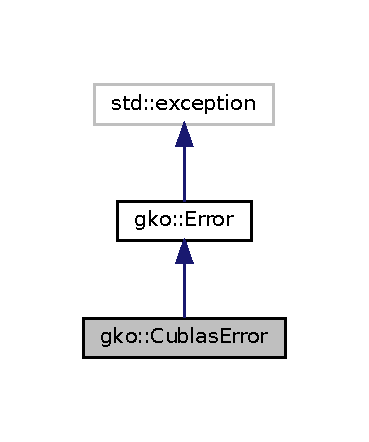
\includegraphics[width=177pt]{classgko_1_1CublasError__coll__graph}
\end{center}
\end{figure}
\subsection*{Public Member Functions}
\begin{DoxyCompactItemize}
\item 
\hyperlink{classgko_1_1CublasError_a4f16cd8a9189da444d11a97337a56d8f}{Cublas\+Error} (const std\+::string \&file, int line, const std\+::string \&func, \hyperlink{namespacegko_a6c57dbf3168b1ecad3ea133aaf2efbc1}{int64} error\+\_\+code)
\begin{DoxyCompactList}\small\item\em Initializes a cu\+B\+L\+AS error. \end{DoxyCompactList}\end{DoxyCompactItemize}


\subsection{Detailed Description}
\hyperlink{classgko_1_1CublasError}{Cublas\+Error} is thrown when a cu\+B\+L\+AS routine throws a non-\/zero error code. 

\subsection{Constructor \& Destructor Documentation}
\mbox{\Hypertarget{classgko_1_1CublasError_a4f16cd8a9189da444d11a97337a56d8f}\label{classgko_1_1CublasError_a4f16cd8a9189da444d11a97337a56d8f}} 
\index{gko\+::\+Cublas\+Error@{gko\+::\+Cublas\+Error}!Cublas\+Error@{Cublas\+Error}}
\index{Cublas\+Error@{Cublas\+Error}!gko\+::\+Cublas\+Error@{gko\+::\+Cublas\+Error}}
\subsubsection{\texorpdfstring{Cublas\+Error()}{CublasError()}}
{\footnotesize\ttfamily gko\+::\+Cublas\+Error\+::\+Cublas\+Error (\begin{DoxyParamCaption}\item[{const std\+::string \&}]{file,  }\item[{int}]{line,  }\item[{const std\+::string \&}]{func,  }\item[{\hyperlink{namespacegko_a6c57dbf3168b1ecad3ea133aaf2efbc1}{int64}}]{error\+\_\+code }\end{DoxyParamCaption})\hspace{0.3cm}{\ttfamily [inline]}}



Initializes a cu\+B\+L\+AS error. 


\begin{DoxyParams}{Parameters}
{\em file} & The name of the offending source file \\
\hline
{\em line} & The source code line number where the error occurred \\
\hline
{\em func} & The name of the cu\+B\+L\+AS routine that failed \\
\hline
{\em error\+\_\+code} & The resulting cu\+B\+L\+AS error code \\
\hline
\end{DoxyParams}


The documentation for this class was generated from the following file\+:\begin{DoxyCompactItemize}
\item 
ginkgo/core/base/exception.\+hpp (c71510aa)\end{DoxyCompactItemize}

\hypertarget{classgko_1_1CudaError}{}\doxysection{gko\+::Cuda\+Error Class Reference}
\label{classgko_1_1CudaError}\index{gko::CudaError@{gko::CudaError}}


\mbox{\hyperlink{classgko_1_1CudaError}{Cuda\+Error}} is thrown when a C\+U\+DA routine throws a non-\/zero error code.  




{\ttfamily \#include $<$ginkgo/core/base/exception.\+hpp$>$}



Collaboration diagram for gko\+::Cuda\+Error\+:
\nopagebreak
\begin{figure}[H]
\begin{center}
\leavevmode
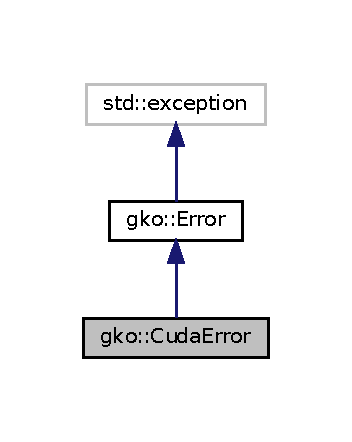
\includegraphics[width=169pt]{classgko_1_1CudaError__coll__graph}
\end{center}
\end{figure}
\doxysubsection*{Public Member Functions}
\begin{DoxyCompactItemize}
\item 
\mbox{\hyperlink{classgko_1_1CudaError_aa4f4d466d2ccdb9da5e331d8dad92d39}{Cuda\+Error}} (const std\+::string \&file, int line, const std\+::string \&func, \mbox{\hyperlink{namespacegko_a6c57dbf3168b1ecad3ea133aaf2efbc1}{int64}} error\+\_\+code)
\begin{DoxyCompactList}\small\item\em Initializes a C\+U\+DA error. \end{DoxyCompactList}\end{DoxyCompactItemize}


\doxysubsection{Detailed Description}
\mbox{\hyperlink{classgko_1_1CudaError}{Cuda\+Error}} is thrown when a C\+U\+DA routine throws a non-\/zero error code. 

\doxysubsection{Constructor \& Destructor Documentation}
\mbox{\Hypertarget{classgko_1_1CudaError_aa4f4d466d2ccdb9da5e331d8dad92d39}\label{classgko_1_1CudaError_aa4f4d466d2ccdb9da5e331d8dad92d39}} 
\index{gko::CudaError@{gko::CudaError}!CudaError@{CudaError}}
\index{CudaError@{CudaError}!gko::CudaError@{gko::CudaError}}
\doxysubsubsection{\texorpdfstring{CudaError()}{CudaError()}}
{\footnotesize\ttfamily gko\+::\+Cuda\+Error\+::\+Cuda\+Error (\begin{DoxyParamCaption}\item[{const std\+::string \&}]{file,  }\item[{int}]{line,  }\item[{const std\+::string \&}]{func,  }\item[{\mbox{\hyperlink{namespacegko_a6c57dbf3168b1ecad3ea133aaf2efbc1}{int64}}}]{error\+\_\+code }\end{DoxyParamCaption})\hspace{0.3cm}{\ttfamily [inline]}}



Initializes a C\+U\+DA error. 


\begin{DoxyParams}{Parameters}
{\em file} & The name of the offending source file \\
\hline
{\em line} & The source code line number where the error occurred \\
\hline
{\em func} & The name of the C\+U\+DA routine that failed \\
\hline
{\em error\+\_\+code} & The resulting C\+U\+DA error code \\
\hline
\end{DoxyParams}


The documentation for this class was generated from the following file\+:\begin{DoxyCompactItemize}
\item 
ginkgo/core/base/exception.\+hpp (ccf35426a)\end{DoxyCompactItemize}

\hypertarget{classgko_1_1CudaExecutor}{}\doxysection{gko\+::Cuda\+Executor Class Reference}
\label{classgko_1_1CudaExecutor}\index{gko::CudaExecutor@{gko::CudaExecutor}}


This is the \mbox{\hyperlink{classgko_1_1Executor}{Executor}} subclass which represents the C\+U\+DA device.  




{\ttfamily \#include $<$ginkgo/core/base/executor.\+hpp$>$}



Collaboration diagram for gko\+::Cuda\+Executor\+:
\nopagebreak
\begin{figure}[H]
\begin{center}
\leavevmode
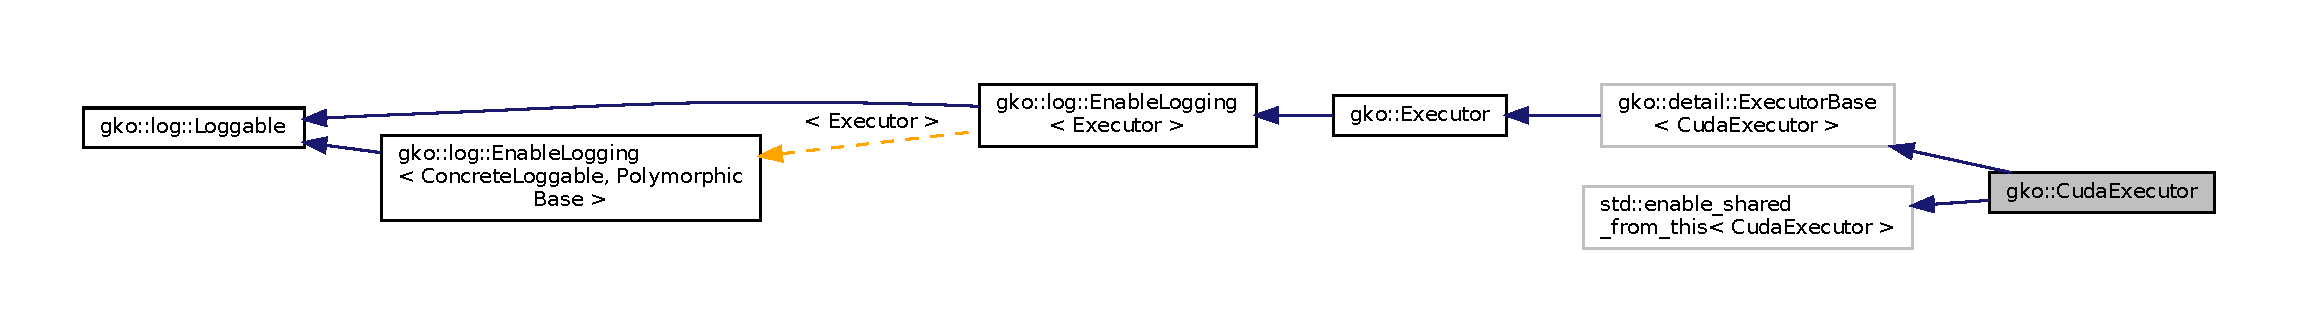
\includegraphics[width=350pt]{classgko_1_1CudaExecutor__coll__graph}
\end{center}
\end{figure}
\doxysubsection*{Public Member Functions}
\begin{DoxyCompactItemize}
\item 
std\+::shared\+\_\+ptr$<$ \mbox{\hyperlink{classgko_1_1Executor}{Executor}} $>$ \mbox{\hyperlink{classgko_1_1CudaExecutor_a59a618e0d48b42fe699e9d4cf347b491}{get\+\_\+master}} () noexcept override
\begin{DoxyCompactList}\small\item\em Returns the master \mbox{\hyperlink{classgko_1_1OmpExecutor}{Omp\+Executor}} of this \mbox{\hyperlink{classgko_1_1Executor}{Executor}}. \end{DoxyCompactList}\item 
std\+::shared\+\_\+ptr$<$ const \mbox{\hyperlink{classgko_1_1Executor}{Executor}} $>$ \mbox{\hyperlink{classgko_1_1CudaExecutor_a75295b3424224f907958abfa95c66298}{get\+\_\+master}} () const noexcept override
\begin{DoxyCompactList}\small\item\em Returns the master \mbox{\hyperlink{classgko_1_1OmpExecutor}{Omp\+Executor}} of this \mbox{\hyperlink{classgko_1_1Executor}{Executor}}. \end{DoxyCompactList}\item 
\mbox{\Hypertarget{classgko_1_1CudaExecutor_a903cf7e3460b14677c0bce5ca08a1b81}\label{classgko_1_1CudaExecutor_a903cf7e3460b14677c0bce5ca08a1b81}} 
void \mbox{\hyperlink{classgko_1_1CudaExecutor_a903cf7e3460b14677c0bce5ca08a1b81}{synchronize}} () const override
\begin{DoxyCompactList}\small\item\em Synchronize the operations launched on the executor with its master. \end{DoxyCompactList}\item 
void \mbox{\hyperlink{classgko_1_1CudaExecutor_a32a73a74403376d774933abf9663d59e}{run}} (const \mbox{\hyperlink{classgko_1_1Operation}{Operation}} \&op) const override
\begin{DoxyCompactList}\small\item\em Runs the specified \mbox{\hyperlink{classgko_1_1Operation}{Operation}} using this \mbox{\hyperlink{classgko_1_1Executor}{Executor}}. \end{DoxyCompactList}\item 
\mbox{\Hypertarget{classgko_1_1CudaExecutor_a7cfa915eadd2329eb897dc1ee2712488}\label{classgko_1_1CudaExecutor_a7cfa915eadd2329eb897dc1ee2712488}} 
int \mbox{\hyperlink{classgko_1_1CudaExecutor_a7cfa915eadd2329eb897dc1ee2712488}{get\+\_\+device\+\_\+id}} () const noexcept
\begin{DoxyCompactList}\small\item\em Get the C\+U\+DA device id of the device associated to this executor. \end{DoxyCompactList}\item 
\mbox{\Hypertarget{classgko_1_1CudaExecutor_a245c1c35a18e6534d87ef6e9cad24f7c}\label{classgko_1_1CudaExecutor_a245c1c35a18e6534d87ef6e9cad24f7c}} 
int \mbox{\hyperlink{classgko_1_1CudaExecutor_a245c1c35a18e6534d87ef6e9cad24f7c}{get\+\_\+num\+\_\+warps\+\_\+per\+\_\+sm}} () const noexcept
\begin{DoxyCompactList}\small\item\em Get the number of warps per SM of this executor. \end{DoxyCompactList}\item 
\mbox{\Hypertarget{classgko_1_1CudaExecutor_a449c2bf9c51b58a04fdb8b4a73377820}\label{classgko_1_1CudaExecutor_a449c2bf9c51b58a04fdb8b4a73377820}} 
int \mbox{\hyperlink{classgko_1_1CudaExecutor_a449c2bf9c51b58a04fdb8b4a73377820}{get\+\_\+num\+\_\+multiprocessor}} () const noexcept
\begin{DoxyCompactList}\small\item\em Get the number of multiprocessor of this executor. \end{DoxyCompactList}\item 
\mbox{\Hypertarget{classgko_1_1CudaExecutor_aa9d77db0b87322a8bef12380029b5310}\label{classgko_1_1CudaExecutor_aa9d77db0b87322a8bef12380029b5310}} 
int \mbox{\hyperlink{classgko_1_1CudaExecutor_aa9d77db0b87322a8bef12380029b5310}{get\+\_\+num\+\_\+warps}} () const noexcept
\begin{DoxyCompactList}\small\item\em Get the number of warps of this executor. \end{DoxyCompactList}\item 
\mbox{\Hypertarget{classgko_1_1CudaExecutor_a6a3894e9f4d98b5f7523e067c88ef521}\label{classgko_1_1CudaExecutor_a6a3894e9f4d98b5f7523e067c88ef521}} 
int \mbox{\hyperlink{classgko_1_1CudaExecutor_a6a3894e9f4d98b5f7523e067c88ef521}{get\+\_\+warp\+\_\+size}} () const noexcept
\begin{DoxyCompactList}\small\item\em Get the warp size of this executor. \end{DoxyCompactList}\item 
\mbox{\Hypertarget{classgko_1_1CudaExecutor_a3868f53f82b6398acb1ba1f9647a6e46}\label{classgko_1_1CudaExecutor_a3868f53f82b6398acb1ba1f9647a6e46}} 
int \mbox{\hyperlink{classgko_1_1CudaExecutor_a3868f53f82b6398acb1ba1f9647a6e46}{get\+\_\+major\+\_\+version}} () const noexcept
\begin{DoxyCompactList}\small\item\em Get the major verion of compute capability. \end{DoxyCompactList}\item 
\mbox{\Hypertarget{classgko_1_1CudaExecutor_aa7d7a5cd7aeb38b8ab8fe3e4d1538481}\label{classgko_1_1CudaExecutor_aa7d7a5cd7aeb38b8ab8fe3e4d1538481}} 
int \mbox{\hyperlink{classgko_1_1CudaExecutor_aa7d7a5cd7aeb38b8ab8fe3e4d1538481}{get\+\_\+minor\+\_\+version}} () const noexcept
\begin{DoxyCompactList}\small\item\em Get the minor verion of compute capability. \end{DoxyCompactList}\item 
cublas\+Context $\ast$ \mbox{\hyperlink{classgko_1_1CudaExecutor_a5b5f8febb914c9984bc77b15e7bb7601}{get\+\_\+cublas\+\_\+handle}} () const
\begin{DoxyCompactList}\small\item\em Get the cublas handle for this executor. \end{DoxyCompactList}\item 
cusparse\+Context $\ast$ \mbox{\hyperlink{classgko_1_1CudaExecutor_ade84197157cc2695e5c94310692ab323}{get\+\_\+cusparse\+\_\+handle}} () const
\begin{DoxyCompactList}\small\item\em Get the cusparse handle for this executor. \end{DoxyCompactList}\end{DoxyCompactItemize}
\doxysubsection*{Static Public Member Functions}
\begin{DoxyCompactItemize}
\item 
static std\+::shared\+\_\+ptr$<$ \mbox{\hyperlink{classgko_1_1CudaExecutor}{Cuda\+Executor}} $>$ \mbox{\hyperlink{classgko_1_1CudaExecutor_a2718a92034350650ef406ffdb60db090}{create}} (int device\+\_\+id, std\+::shared\+\_\+ptr$<$ \mbox{\hyperlink{classgko_1_1Executor}{Executor}} $>$ master)
\begin{DoxyCompactList}\small\item\em Creates a new \mbox{\hyperlink{classgko_1_1CudaExecutor}{Cuda\+Executor}}. \end{DoxyCompactList}\item 
\mbox{\Hypertarget{classgko_1_1CudaExecutor_aef0258494d14de0e56149b920c5173e5}\label{classgko_1_1CudaExecutor_aef0258494d14de0e56149b920c5173e5}} 
static int \mbox{\hyperlink{classgko_1_1CudaExecutor_aef0258494d14de0e56149b920c5173e5}{get\+\_\+num\+\_\+devices}} ()
\begin{DoxyCompactList}\small\item\em Get the number of devices present on the system. \end{DoxyCompactList}\end{DoxyCompactItemize}


\doxysubsection{Detailed Description}
This is the \mbox{\hyperlink{classgko_1_1Executor}{Executor}} subclass which represents the C\+U\+DA device. 

\doxysubsection{Member Function Documentation}
\mbox{\Hypertarget{classgko_1_1CudaExecutor_a2718a92034350650ef406ffdb60db090}\label{classgko_1_1CudaExecutor_a2718a92034350650ef406ffdb60db090}} 
\index{gko::CudaExecutor@{gko::CudaExecutor}!create@{create}}
\index{create@{create}!gko::CudaExecutor@{gko::CudaExecutor}}
\doxysubsubsection{\texorpdfstring{create()}{create()}}
{\footnotesize\ttfamily static std\+::shared\+\_\+ptr$<$\mbox{\hyperlink{classgko_1_1CudaExecutor}{Cuda\+Executor}}$>$ gko\+::\+Cuda\+Executor\+::create (\begin{DoxyParamCaption}\item[{int}]{device\+\_\+id,  }\item[{std\+::shared\+\_\+ptr$<$ \mbox{\hyperlink{classgko_1_1Executor}{Executor}} $>$}]{master }\end{DoxyParamCaption})\hspace{0.3cm}{\ttfamily [static]}}



Creates a new \mbox{\hyperlink{classgko_1_1CudaExecutor}{Cuda\+Executor}}. 


\begin{DoxyParams}{Parameters}
{\em device\+\_\+id} & the C\+U\+DA device id of this device \\
\hline
{\em master} & an executor on the host that is used to invoke the device kernels \\
\hline
\end{DoxyParams}
\mbox{\Hypertarget{classgko_1_1CudaExecutor_a5b5f8febb914c9984bc77b15e7bb7601}\label{classgko_1_1CudaExecutor_a5b5f8febb914c9984bc77b15e7bb7601}} 
\index{gko::CudaExecutor@{gko::CudaExecutor}!get\_cublas\_handle@{get\_cublas\_handle}}
\index{get\_cublas\_handle@{get\_cublas\_handle}!gko::CudaExecutor@{gko::CudaExecutor}}
\doxysubsubsection{\texorpdfstring{get\_cublas\_handle()}{get\_cublas\_handle()}}
{\footnotesize\ttfamily cublas\+Context$\ast$ gko\+::\+Cuda\+Executor\+::get\+\_\+cublas\+\_\+handle (\begin{DoxyParamCaption}{ }\end{DoxyParamCaption}) const\hspace{0.3cm}{\ttfamily [inline]}}



Get the cublas handle for this executor. 

\begin{DoxyReturn}{Returns}
the cublas handle (cublas\+Context$\ast$) for this executor 
\end{DoxyReturn}
\mbox{\Hypertarget{classgko_1_1CudaExecutor_ade84197157cc2695e5c94310692ab323}\label{classgko_1_1CudaExecutor_ade84197157cc2695e5c94310692ab323}} 
\index{gko::CudaExecutor@{gko::CudaExecutor}!get\_cusparse\_handle@{get\_cusparse\_handle}}
\index{get\_cusparse\_handle@{get\_cusparse\_handle}!gko::CudaExecutor@{gko::CudaExecutor}}
\doxysubsubsection{\texorpdfstring{get\_cusparse\_handle()}{get\_cusparse\_handle()}}
{\footnotesize\ttfamily cusparse\+Context$\ast$ gko\+::\+Cuda\+Executor\+::get\+\_\+cusparse\+\_\+handle (\begin{DoxyParamCaption}{ }\end{DoxyParamCaption}) const\hspace{0.3cm}{\ttfamily [inline]}}



Get the cusparse handle for this executor. 

\begin{DoxyReturn}{Returns}
the cusparse handle (cusparse\+Context$\ast$) for this executor 
\end{DoxyReturn}
\mbox{\Hypertarget{classgko_1_1CudaExecutor_a75295b3424224f907958abfa95c66298}\label{classgko_1_1CudaExecutor_a75295b3424224f907958abfa95c66298}} 
\index{gko::CudaExecutor@{gko::CudaExecutor}!get\_master@{get\_master}}
\index{get\_master@{get\_master}!gko::CudaExecutor@{gko::CudaExecutor}}
\doxysubsubsection{\texorpdfstring{get\_master()}{get\_master()}\hspace{0.1cm}{\footnotesize\ttfamily [1/2]}}
{\footnotesize\ttfamily std\+::shared\+\_\+ptr$<$const \mbox{\hyperlink{classgko_1_1Executor}{Executor}}$>$ gko\+::\+Cuda\+Executor\+::get\+\_\+master (\begin{DoxyParamCaption}{ }\end{DoxyParamCaption}) const\hspace{0.3cm}{\ttfamily [override]}, {\ttfamily [virtual]}, {\ttfamily [noexcept]}}



Returns the master \mbox{\hyperlink{classgko_1_1OmpExecutor}{Omp\+Executor}} of this \mbox{\hyperlink{classgko_1_1Executor}{Executor}}. 

\begin{DoxyReturn}{Returns}
the master \mbox{\hyperlink{classgko_1_1OmpExecutor}{Omp\+Executor}} of this \mbox{\hyperlink{classgko_1_1Executor}{Executor}}. 
\end{DoxyReturn}


Implements \mbox{\hyperlink{classgko_1_1Executor_a261386e439c8daa6e0d95dc331b9bfeb}{gko\+::\+Executor}}.

\mbox{\Hypertarget{classgko_1_1CudaExecutor_a59a618e0d48b42fe699e9d4cf347b491}\label{classgko_1_1CudaExecutor_a59a618e0d48b42fe699e9d4cf347b491}} 
\index{gko::CudaExecutor@{gko::CudaExecutor}!get\_master@{get\_master}}
\index{get\_master@{get\_master}!gko::CudaExecutor@{gko::CudaExecutor}}
\doxysubsubsection{\texorpdfstring{get\_master()}{get\_master()}\hspace{0.1cm}{\footnotesize\ttfamily [2/2]}}
{\footnotesize\ttfamily std\+::shared\+\_\+ptr$<$\mbox{\hyperlink{classgko_1_1Executor}{Executor}}$>$ gko\+::\+Cuda\+Executor\+::get\+\_\+master (\begin{DoxyParamCaption}{ }\end{DoxyParamCaption})\hspace{0.3cm}{\ttfamily [override]}, {\ttfamily [virtual]}, {\ttfamily [noexcept]}}



Returns the master \mbox{\hyperlink{classgko_1_1OmpExecutor}{Omp\+Executor}} of this \mbox{\hyperlink{classgko_1_1Executor}{Executor}}. 

\begin{DoxyReturn}{Returns}
the master \mbox{\hyperlink{classgko_1_1OmpExecutor}{Omp\+Executor}} of this \mbox{\hyperlink{classgko_1_1Executor}{Executor}}. 
\end{DoxyReturn}


Implements \mbox{\hyperlink{classgko_1_1Executor_acaec4f999d52fc71e5e5a3d3ad93609c}{gko\+::\+Executor}}.

\mbox{\Hypertarget{classgko_1_1CudaExecutor_a32a73a74403376d774933abf9663d59e}\label{classgko_1_1CudaExecutor_a32a73a74403376d774933abf9663d59e}} 
\index{gko::CudaExecutor@{gko::CudaExecutor}!run@{run}}
\index{run@{run}!gko::CudaExecutor@{gko::CudaExecutor}}
\doxysubsubsection{\texorpdfstring{run()}{run()}}
{\footnotesize\ttfamily void gko\+::\+Cuda\+Executor\+::run (\begin{DoxyParamCaption}\item[{const \mbox{\hyperlink{classgko_1_1Operation}{Operation}} \&}]{op }\end{DoxyParamCaption}) const\hspace{0.3cm}{\ttfamily [override]}, {\ttfamily [virtual]}}



Runs the specified \mbox{\hyperlink{classgko_1_1Operation}{Operation}} using this \mbox{\hyperlink{classgko_1_1Executor}{Executor}}. 


\begin{DoxyParams}{Parameters}
{\em op} & the operation to run \\
\hline
\end{DoxyParams}


Implements \mbox{\hyperlink{classgko_1_1Executor_a1de8e2668b76e66690acf5eef9e8324d}{gko\+::\+Executor}}.



The documentation for this class was generated from the following file\+:\begin{DoxyCompactItemize}
\item 
ginkgo/core/base/executor.\+hpp (8e9aa9083)\end{DoxyCompactItemize}

\hypertarget{classgko_1_1matrix_1_1Csr_1_1cusparse}{}\doxysection{gko\+::matrix\+::Csr$<$ Value\+Type, Index\+Type $>$\+::cusparse Class Reference}
\label{classgko_1_1matrix_1_1Csr_1_1cusparse}\index{gko::matrix::Csr$<$ ValueType, IndexType $>$::cusparse@{gko::matrix::Csr$<$ ValueType, IndexType $>$::cusparse}}


cusparse is a \mbox{\hyperlink{classgko_1_1matrix_1_1Csr_1_1strategy__type}{strategy\+\_\+type}} which uses the sparselib csr.  




{\ttfamily \#include $<$ginkgo/core/matrix/csr.\+hpp$>$}



Collaboration diagram for gko\+::matrix\+::Csr$<$ Value\+Type, Index\+Type $>$\+::cusparse\+:
\nopagebreak
\begin{figure}[H]
\begin{center}
\leavevmode
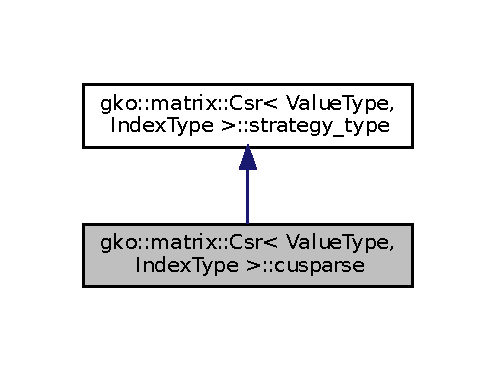
\includegraphics[width=238pt]{classgko_1_1matrix_1_1Csr_1_1cusparse__coll__graph}
\end{center}
\end{figure}
\doxysubsection*{Public Member Functions}
\begin{DoxyCompactItemize}
\item 
\mbox{\Hypertarget{classgko_1_1matrix_1_1Csr_1_1cusparse_a9aae722e5f5838291bf1f1798277a83c}\label{classgko_1_1matrix_1_1Csr_1_1cusparse_a9aae722e5f5838291bf1f1798277a83c}} 
\mbox{\hyperlink{classgko_1_1matrix_1_1Csr_1_1cusparse_a9aae722e5f5838291bf1f1798277a83c}{cusparse}} ()
\begin{DoxyCompactList}\small\item\em Creates a cusparse strategy. \end{DoxyCompactList}\item 
void \mbox{\hyperlink{classgko_1_1matrix_1_1Csr_1_1cusparse_acf64bdc81eee1fb3f46fd80f5d920939}{process}} (const \mbox{\hyperlink{classgko_1_1Array}{Array}}$<$ index\+\_\+type $>$ \&mtx\+\_\+row\+\_\+ptrs, \mbox{\hyperlink{classgko_1_1Array}{Array}}$<$ index\+\_\+type $>$ $\ast$mtx\+\_\+srow) override
\begin{DoxyCompactList}\small\item\em Computes srow according to row pointers. \end{DoxyCompactList}\item 
int64\+\_\+t \mbox{\hyperlink{classgko_1_1matrix_1_1Csr_1_1cusparse_a094614c818d821cb0a71a4266fbef2d0}{clac\+\_\+size}} (const int64\+\_\+t nnz) override
\begin{DoxyCompactList}\small\item\em Computes the srow size according to the number of nonzeros. \end{DoxyCompactList}\item 
std\+::shared\+\_\+ptr$<$ \mbox{\hyperlink{classgko_1_1matrix_1_1Csr_1_1strategy__type}{strategy\+\_\+type}} $>$ \mbox{\hyperlink{classgko_1_1matrix_1_1Csr_1_1cusparse_aaa34a27d6d9fb0d7bef655ad9a4fc686}{copy}} () override
\begin{DoxyCompactList}\small\item\em Copy a strategy. \end{DoxyCompactList}\end{DoxyCompactItemize}


\doxysubsection{Detailed Description}
\subsubsection*{template$<$typename Value\+Type = default\+\_\+precision, typename Index\+Type = int32$>$\newline
class gko\+::matrix\+::\+Csr$<$ Value\+Type, Index\+Type $>$\+::cusparse}

cusparse is a \mbox{\hyperlink{classgko_1_1matrix_1_1Csr_1_1strategy__type}{strategy\+\_\+type}} which uses the sparselib csr. 

\begin{DoxyNote}{Note}
cusparse is also known to the hip executor which converts between cuda and hip. 
\end{DoxyNote}


\doxysubsection{Member Function Documentation}
\mbox{\Hypertarget{classgko_1_1matrix_1_1Csr_1_1cusparse_a094614c818d821cb0a71a4266fbef2d0}\label{classgko_1_1matrix_1_1Csr_1_1cusparse_a094614c818d821cb0a71a4266fbef2d0}} 
\index{gko::matrix::Csr$<$ ValueType, IndexType $>$::cusparse@{gko::matrix::Csr$<$ ValueType, IndexType $>$::cusparse}!clac\_size@{clac\_size}}
\index{clac\_size@{clac\_size}!gko::matrix::Csr$<$ ValueType, IndexType $>$::cusparse@{gko::matrix::Csr$<$ ValueType, IndexType $>$::cusparse}}
\doxysubsubsection{\texorpdfstring{clac\_size()}{clac\_size()}}
{\footnotesize\ttfamily template$<$typename Value\+Type = default\+\_\+precision, typename Index\+Type = int32$>$ \\
int64\+\_\+t \mbox{\hyperlink{classgko_1_1matrix_1_1Csr}{gko\+::matrix\+::\+Csr}}$<$ Value\+Type, Index\+Type $>$\+::cusparse\+::clac\+\_\+size (\begin{DoxyParamCaption}\item[{const int64\+\_\+t}]{nnz }\end{DoxyParamCaption})\hspace{0.3cm}{\ttfamily [inline]}, {\ttfamily [override]}, {\ttfamily [virtual]}}



Computes the srow size according to the number of nonzeros. 


\begin{DoxyParams}{Parameters}
{\em nnz} & the number of nonzeros\\
\hline
\end{DoxyParams}
\begin{DoxyReturn}{Returns}
the size of srow 
\end{DoxyReturn}


Implements \mbox{\hyperlink{classgko_1_1matrix_1_1Csr_1_1strategy__type_a07a6dda9dd04ed8abd914f3a69f330f2}{gko\+::matrix\+::\+Csr$<$ Value\+Type, Index\+Type $>$\+::strategy\+\_\+type}}.

\mbox{\Hypertarget{classgko_1_1matrix_1_1Csr_1_1cusparse_aaa34a27d6d9fb0d7bef655ad9a4fc686}\label{classgko_1_1matrix_1_1Csr_1_1cusparse_aaa34a27d6d9fb0d7bef655ad9a4fc686}} 
\index{gko::matrix::Csr$<$ ValueType, IndexType $>$::cusparse@{gko::matrix::Csr$<$ ValueType, IndexType $>$::cusparse}!copy@{copy}}
\index{copy@{copy}!gko::matrix::Csr$<$ ValueType, IndexType $>$::cusparse@{gko::matrix::Csr$<$ ValueType, IndexType $>$::cusparse}}
\doxysubsubsection{\texorpdfstring{copy()}{copy()}}
{\footnotesize\ttfamily template$<$typename Value\+Type = default\+\_\+precision, typename Index\+Type = int32$>$ \\
std\+::shared\+\_\+ptr$<$\mbox{\hyperlink{classgko_1_1matrix_1_1Csr_1_1strategy__type}{strategy\+\_\+type}}$>$ \mbox{\hyperlink{classgko_1_1matrix_1_1Csr}{gko\+::matrix\+::\+Csr}}$<$ Value\+Type, Index\+Type $>$\+::cusparse\+::copy (\begin{DoxyParamCaption}{ }\end{DoxyParamCaption})\hspace{0.3cm}{\ttfamily [inline]}, {\ttfamily [override]}, {\ttfamily [virtual]}}



Copy a strategy. 

This is a workaround until strategies are revamped, since strategies like {\ttfamily automatical} do not work when actually shared. 

Implements \mbox{\hyperlink{classgko_1_1matrix_1_1Csr_1_1strategy__type_adf3dc78938ffb991608b272447db6a68}{gko\+::matrix\+::\+Csr$<$ Value\+Type, Index\+Type $>$\+::strategy\+\_\+type}}.

\mbox{\Hypertarget{classgko_1_1matrix_1_1Csr_1_1cusparse_acf64bdc81eee1fb3f46fd80f5d920939}\label{classgko_1_1matrix_1_1Csr_1_1cusparse_acf64bdc81eee1fb3f46fd80f5d920939}} 
\index{gko::matrix::Csr$<$ ValueType, IndexType $>$::cusparse@{gko::matrix::Csr$<$ ValueType, IndexType $>$::cusparse}!process@{process}}
\index{process@{process}!gko::matrix::Csr$<$ ValueType, IndexType $>$::cusparse@{gko::matrix::Csr$<$ ValueType, IndexType $>$::cusparse}}
\doxysubsubsection{\texorpdfstring{process()}{process()}}
{\footnotesize\ttfamily template$<$typename Value\+Type = default\+\_\+precision, typename Index\+Type = int32$>$ \\
void \mbox{\hyperlink{classgko_1_1matrix_1_1Csr}{gko\+::matrix\+::\+Csr}}$<$ Value\+Type, Index\+Type $>$\+::cusparse\+::process (\begin{DoxyParamCaption}\item[{const \mbox{\hyperlink{classgko_1_1Array}{Array}}$<$ index\+\_\+type $>$ \&}]{mtx\+\_\+row\+\_\+ptrs,  }\item[{\mbox{\hyperlink{classgko_1_1Array}{Array}}$<$ index\+\_\+type $>$ $\ast$}]{mtx\+\_\+srow }\end{DoxyParamCaption})\hspace{0.3cm}{\ttfamily [inline]}, {\ttfamily [override]}, {\ttfamily [virtual]}}



Computes srow according to row pointers. 


\begin{DoxyParams}{Parameters}
{\em mtx\+\_\+row\+\_\+ptrs} & the row pointers of the matrix \\
\hline
{\em mtx\+\_\+srow} & the srow of the matrix \\
\hline
\end{DoxyParams}


Implements \mbox{\hyperlink{classgko_1_1matrix_1_1Csr_1_1strategy__type_a58bda9208766e57d861262d4059b65b4}{gko\+::matrix\+::\+Csr$<$ Value\+Type, Index\+Type $>$\+::strategy\+\_\+type}}.



The documentation for this class was generated from the following file\+:\begin{DoxyCompactItemize}
\item 
ginkgo/core/matrix/csr.\+hpp (11a5c086c)\end{DoxyCompactItemize}

\hypertarget{classgko_1_1CusparseError}{}\doxysection{gko\+::Cusparse\+Error Class Reference}
\label{classgko_1_1CusparseError}\index{gko::CusparseError@{gko::CusparseError}}


\mbox{\hyperlink{classgko_1_1CusparseError}{Cusparse\+Error}} is thrown when a cu\+S\+P\+A\+R\+SE routine throws a non-\/zero error code.  




{\ttfamily \#include $<$ginkgo/core/base/exception.\+hpp$>$}



Collaboration diagram for gko\+::Cusparse\+Error\+:
\nopagebreak
\begin{figure}[H]
\begin{center}
\leavevmode
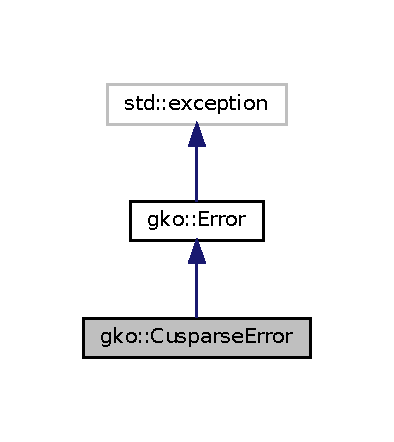
\includegraphics[width=189pt]{classgko_1_1CusparseError__coll__graph}
\end{center}
\end{figure}
\doxysubsection*{Public Member Functions}
\begin{DoxyCompactItemize}
\item 
\mbox{\hyperlink{classgko_1_1CusparseError_ad51ca5caecfc2e41bd06c779d2ca57ae}{Cusparse\+Error}} (const std\+::string \&file, int line, const std\+::string \&func, \mbox{\hyperlink{namespacegko_a6c57dbf3168b1ecad3ea133aaf2efbc1}{int64}} error\+\_\+code)
\begin{DoxyCompactList}\small\item\em Initializes a cu\+S\+P\+A\+R\+SE error. \end{DoxyCompactList}\end{DoxyCompactItemize}


\doxysubsection{Detailed Description}
\mbox{\hyperlink{classgko_1_1CusparseError}{Cusparse\+Error}} is thrown when a cu\+S\+P\+A\+R\+SE routine throws a non-\/zero error code. 

\doxysubsection{Constructor \& Destructor Documentation}
\mbox{\Hypertarget{classgko_1_1CusparseError_ad51ca5caecfc2e41bd06c779d2ca57ae}\label{classgko_1_1CusparseError_ad51ca5caecfc2e41bd06c779d2ca57ae}} 
\index{gko::CusparseError@{gko::CusparseError}!CusparseError@{CusparseError}}
\index{CusparseError@{CusparseError}!gko::CusparseError@{gko::CusparseError}}
\doxysubsubsection{\texorpdfstring{CusparseError()}{CusparseError()}}
{\footnotesize\ttfamily gko\+::\+Cusparse\+Error\+::\+Cusparse\+Error (\begin{DoxyParamCaption}\item[{const std\+::string \&}]{file,  }\item[{int}]{line,  }\item[{const std\+::string \&}]{func,  }\item[{\mbox{\hyperlink{namespacegko_a6c57dbf3168b1ecad3ea133aaf2efbc1}{int64}}}]{error\+\_\+code }\end{DoxyParamCaption})\hspace{0.3cm}{\ttfamily [inline]}}



Initializes a cu\+S\+P\+A\+R\+SE error. 


\begin{DoxyParams}{Parameters}
{\em file} & The name of the offending source file \\
\hline
{\em line} & The source code line number where the error occurred \\
\hline
{\em func} & The name of the cu\+S\+P\+A\+R\+SE routine that failed \\
\hline
{\em error\+\_\+code} & The resulting cu\+S\+P\+A\+R\+SE error code \\
\hline
\end{DoxyParams}


The documentation for this class was generated from the following file\+:\begin{DoxyCompactItemize}
\item 
ginkgo/core/base/exception.\+hpp (29444d385)\end{DoxyCompactItemize}

\hypertarget{structgko_1_1default__converter}{}\doxysection{gko\+::default\+\_\+converter$<$ S, R $>$ Struct Template Reference}
\label{structgko_1_1default__converter}\index{gko::default\_converter$<$ S, R $>$@{gko::default\_converter$<$ S, R $>$}}


Used to convert objects of type {\ttfamily S} to objects of type {\ttfamily R} using static\+\_\+cast.  




{\ttfamily \#include $<$ginkgo/core/base/math.\+hpp$>$}

\doxysubsection*{Public Member Functions}
\begin{DoxyCompactItemize}
\item 
R \mbox{\hyperlink{structgko_1_1default__converter_aeeb535f41abb975f20857989c8ac2470}{operator()}} (S val)
\begin{DoxyCompactList}\small\item\em Converts the object to result type. \end{DoxyCompactList}\end{DoxyCompactItemize}


\doxysubsection{Detailed Description}
\subsubsection*{template$<$typename S, typename R$>$\newline
struct gko\+::default\+\_\+converter$<$ S, R $>$}

Used to convert objects of type {\ttfamily S} to objects of type {\ttfamily R} using static\+\_\+cast. 


\begin{DoxyTemplParams}{Template Parameters}
{\em S} & source type \\
\hline
{\em R} & result type \\
\hline
\end{DoxyTemplParams}


\doxysubsection{Member Function Documentation}
\mbox{\Hypertarget{structgko_1_1default__converter_aeeb535f41abb975f20857989c8ac2470}\label{structgko_1_1default__converter_aeeb535f41abb975f20857989c8ac2470}} 
\index{gko::default\_converter$<$ S, R $>$@{gko::default\_converter$<$ S, R $>$}!operator()@{operator()}}
\index{operator()@{operator()}!gko::default\_converter$<$ S, R $>$@{gko::default\_converter$<$ S, R $>$}}
\doxysubsubsection{\texorpdfstring{operator()()}{operator()()}}
{\footnotesize\ttfamily template$<$typename S , typename R $>$ \\
R \mbox{\hyperlink{structgko_1_1default__converter}{gko\+::default\+\_\+converter}}$<$ S, R $>$\+::operator() (\begin{DoxyParamCaption}\item[{S}]{val }\end{DoxyParamCaption})\hspace{0.3cm}{\ttfamily [inline]}}



Converts the object to result type. 


\begin{DoxyParams}{Parameters}
{\em val} & the object to convert \\
\hline
\end{DoxyParams}
\begin{DoxyReturn}{Returns}
the converted object 
\end{DoxyReturn}


The documentation for this struct was generated from the following file\+:\begin{DoxyCompactItemize}
\item 
ginkgo/core/base/math.\+hpp (4e82207f5)\end{DoxyCompactItemize}

\hypertarget{classgko_1_1matrix_1_1Dense}{}\doxysection{gko\+::matrix\+::Dense$<$ Value\+Type $>$ Class Template Reference}
\label{classgko_1_1matrix_1_1Dense}\index{gko::matrix::Dense$<$ ValueType $>$@{gko::matrix::Dense$<$ ValueType $>$}}


\mbox{\hyperlink{classgko_1_1matrix_1_1Dense}{Dense}} is a matrix format which explicitly stores all values of the matrix.  




{\ttfamily \#include $<$ginkgo/core/matrix/dense.\+hpp$>$}



Collaboration diagram for gko\+::matrix\+::Dense$<$ Value\+Type $>$\+:
\nopagebreak
\begin{figure}[H]
\begin{center}
\leavevmode
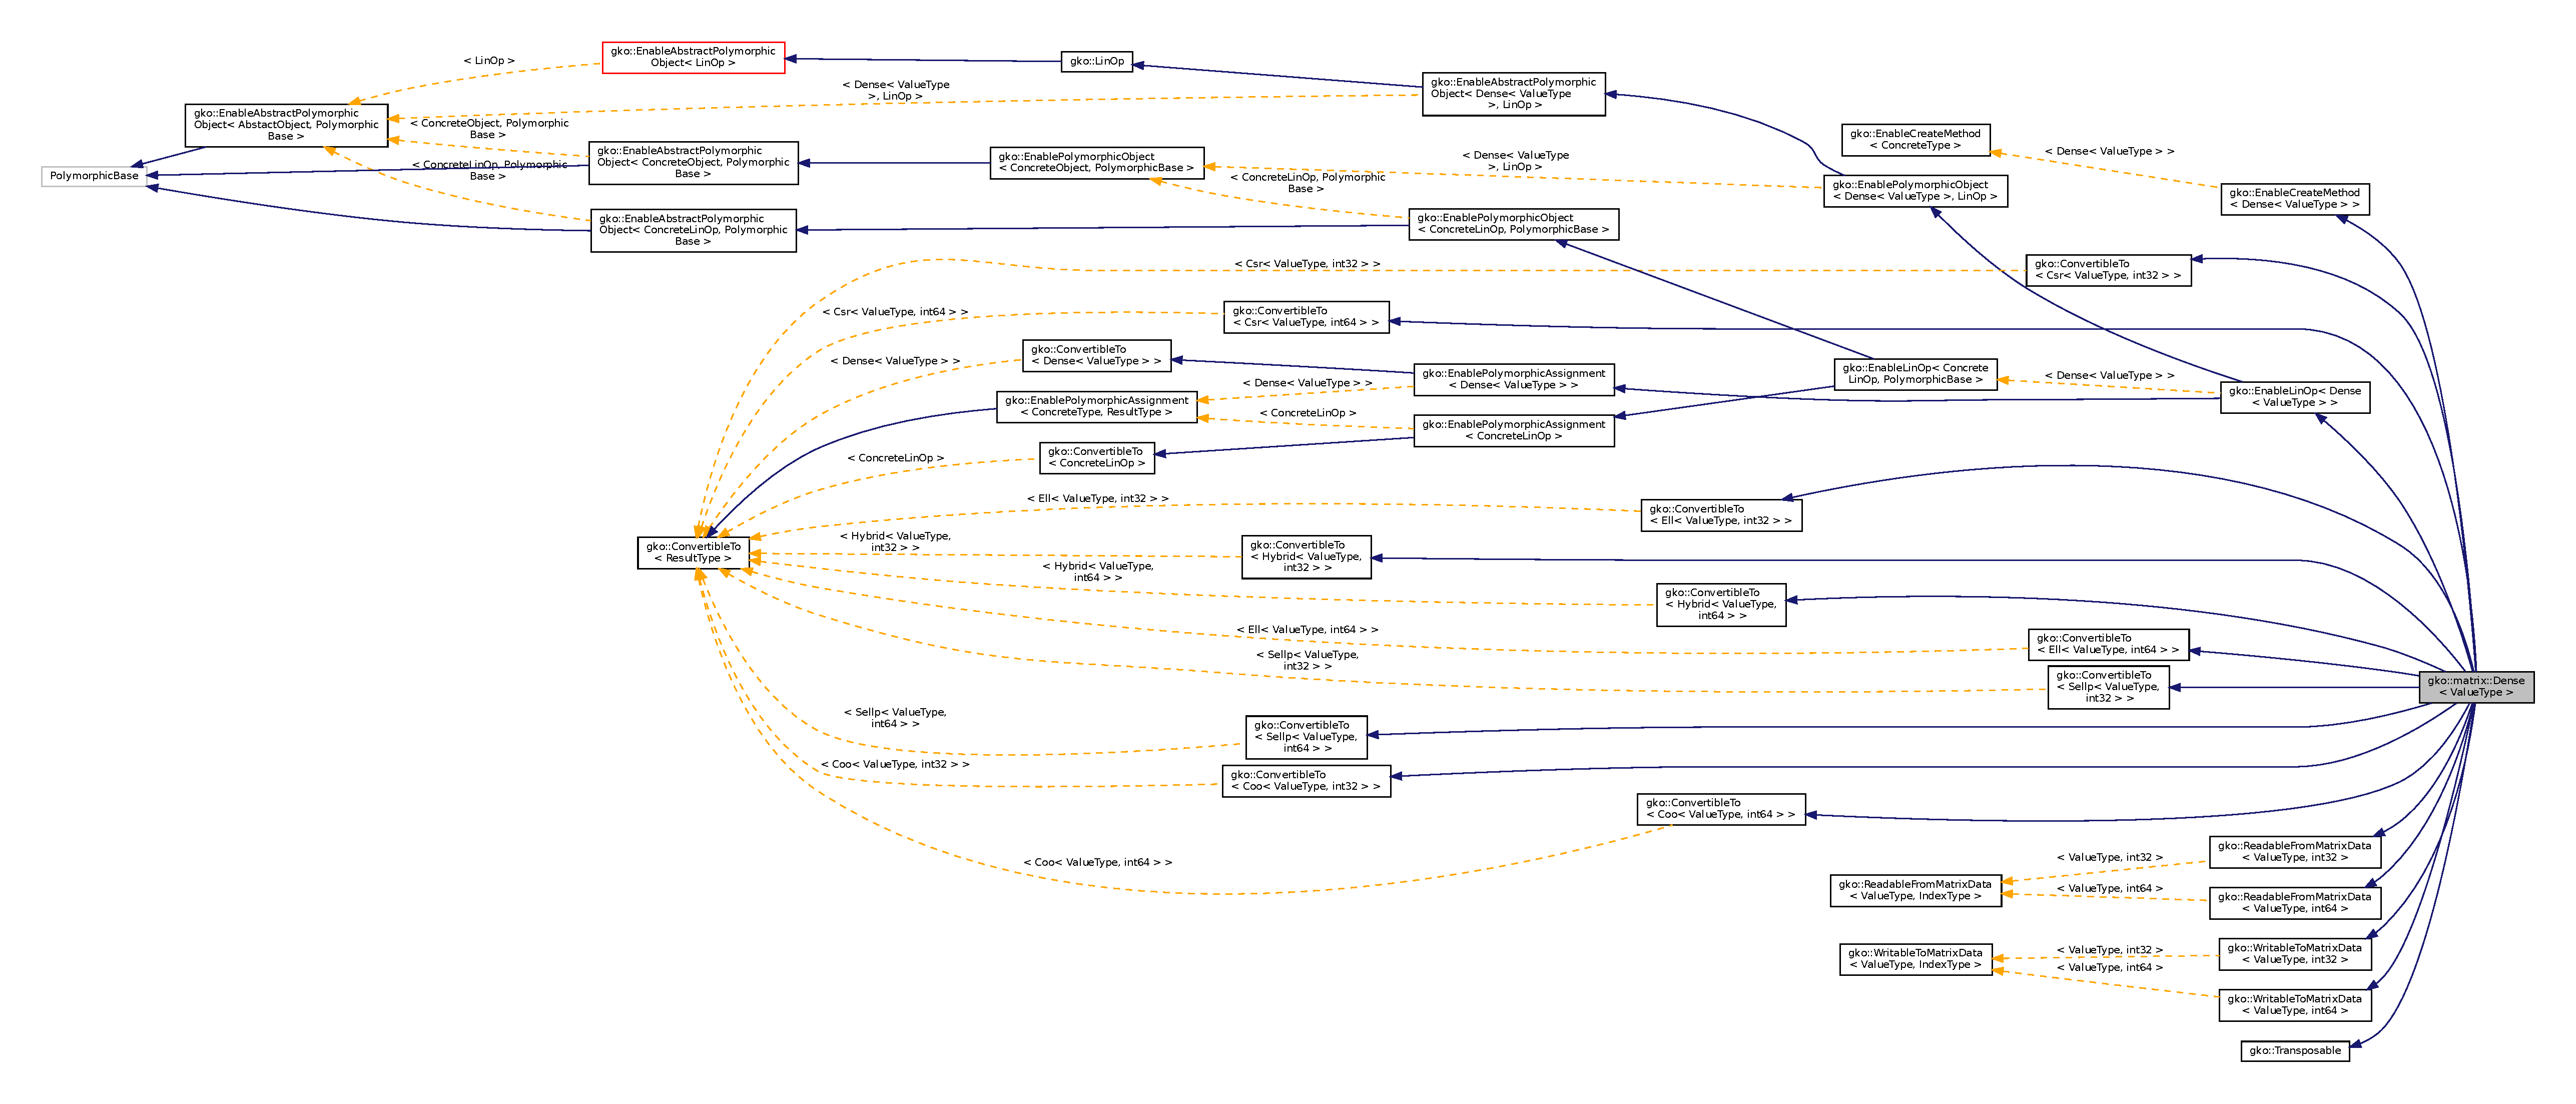
\includegraphics[width=350pt]{classgko_1_1matrix_1_1Dense__coll__graph}
\end{center}
\end{figure}
\doxysubsection*{Public Types}
\begin{DoxyCompactItemize}
\item 
\mbox{\Hypertarget{classgko_1_1matrix_1_1Dense_aa81a0b3798d10eb503eedd9c7ae658b5}\label{classgko_1_1matrix_1_1Dense_aa81a0b3798d10eb503eedd9c7ae658b5}} 
using {\bfseries value\+\_\+type} = Value\+Type
\item 
\mbox{\Hypertarget{classgko_1_1matrix_1_1Dense_a48f92e035bf16c24ed664915f6648163}\label{classgko_1_1matrix_1_1Dense_a48f92e035bf16c24ed664915f6648163}} 
using {\bfseries index\+\_\+type} = \mbox{\hyperlink{namespacegko_a6c57dbf3168b1ecad3ea133aaf2efbc1}{int64}}
\item 
\mbox{\Hypertarget{classgko_1_1matrix_1_1Dense_af3433222c8e30256d79f8984238921f4}\label{classgko_1_1matrix_1_1Dense_af3433222c8e30256d79f8984238921f4}} 
using {\bfseries mat\+\_\+data} = \mbox{\hyperlink{structgko_1_1matrix__data}{gko\+::matrix\+\_\+data}}$<$ Value\+Type, \mbox{\hyperlink{namespacegko_a6c57dbf3168b1ecad3ea133aaf2efbc1}{int64}} $>$
\item 
\mbox{\Hypertarget{classgko_1_1matrix_1_1Dense_a61214ecfce8de48207d1e291beb81c61}\label{classgko_1_1matrix_1_1Dense_a61214ecfce8de48207d1e291beb81c61}} 
using {\bfseries mat\+\_\+data32} = \mbox{\hyperlink{structgko_1_1matrix__data}{gko\+::matrix\+\_\+data}}$<$ Value\+Type, \mbox{\hyperlink{namespacegko_a1ec26caa2379a21a8d0cde611559fff6}{int32}} $>$
\item 
\mbox{\Hypertarget{classgko_1_1matrix_1_1Dense_a67dd271e69cd4ca2942f4cf236fb328e}\label{classgko_1_1matrix_1_1Dense_a67dd271e69cd4ca2942f4cf236fb328e}} 
using {\bfseries row\+\_\+major\+\_\+range} = \mbox{\hyperlink{classgko_1_1range}{gko\+::range}}$<$ \mbox{\hyperlink{classgko_1_1accessor_1_1row__major}{gko\+::accessor\+::row\+\_\+major}}$<$ Value\+Type, 2 $>$ $>$
\end{DoxyCompactItemize}
\doxysubsection*{Public Member Functions}
\begin{DoxyCompactItemize}
\item 
\mbox{\Hypertarget{classgko_1_1matrix_1_1Dense_adaaa152f7bf3566d858a2c81220329a3}\label{classgko_1_1matrix_1_1Dense_adaaa152f7bf3566d858a2c81220329a3}} 
void {\bfseries convert\+\_\+to} (\mbox{\hyperlink{classgko_1_1matrix_1_1Coo}{Coo}}$<$ Value\+Type, \mbox{\hyperlink{namespacegko_a1ec26caa2379a21a8d0cde611559fff6}{int32}} $>$ $\ast$result) const override
\item 
\mbox{\Hypertarget{classgko_1_1matrix_1_1Dense_abff1b9260efc76c7bf1f0fe9831ddf6b}\label{classgko_1_1matrix_1_1Dense_abff1b9260efc76c7bf1f0fe9831ddf6b}} 
void {\bfseries move\+\_\+to} (\mbox{\hyperlink{classgko_1_1matrix_1_1Coo}{Coo}}$<$ Value\+Type, \mbox{\hyperlink{namespacegko_a1ec26caa2379a21a8d0cde611559fff6}{int32}} $>$ $\ast$result) override
\item 
\mbox{\Hypertarget{classgko_1_1matrix_1_1Dense_af231fda06f31db0bd8d7c7bbe2ad428e}\label{classgko_1_1matrix_1_1Dense_af231fda06f31db0bd8d7c7bbe2ad428e}} 
void {\bfseries convert\+\_\+to} (\mbox{\hyperlink{classgko_1_1matrix_1_1Coo}{Coo}}$<$ Value\+Type, \mbox{\hyperlink{namespacegko_a6c57dbf3168b1ecad3ea133aaf2efbc1}{int64}} $>$ $\ast$result) const override
\item 
\mbox{\Hypertarget{classgko_1_1matrix_1_1Dense_ac98a4016b066bcf524b7d391c01b69e6}\label{classgko_1_1matrix_1_1Dense_ac98a4016b066bcf524b7d391c01b69e6}} 
void {\bfseries move\+\_\+to} (\mbox{\hyperlink{classgko_1_1matrix_1_1Coo}{Coo}}$<$ Value\+Type, \mbox{\hyperlink{namespacegko_a6c57dbf3168b1ecad3ea133aaf2efbc1}{int64}} $>$ $\ast$result) override
\item 
\mbox{\Hypertarget{classgko_1_1matrix_1_1Dense_a78d637e4687f6b82380c0f690a0030b9}\label{classgko_1_1matrix_1_1Dense_a78d637e4687f6b82380c0f690a0030b9}} 
void {\bfseries convert\+\_\+to} (\mbox{\hyperlink{classgko_1_1matrix_1_1Csr}{Csr}}$<$ Value\+Type, \mbox{\hyperlink{namespacegko_a1ec26caa2379a21a8d0cde611559fff6}{int32}} $>$ $\ast$result) const override
\item 
\mbox{\Hypertarget{classgko_1_1matrix_1_1Dense_af5cd43fb7c68506437bbc168e160db3d}\label{classgko_1_1matrix_1_1Dense_af5cd43fb7c68506437bbc168e160db3d}} 
void {\bfseries move\+\_\+to} (\mbox{\hyperlink{classgko_1_1matrix_1_1Csr}{Csr}}$<$ Value\+Type, \mbox{\hyperlink{namespacegko_a1ec26caa2379a21a8d0cde611559fff6}{int32}} $>$ $\ast$result) override
\item 
\mbox{\Hypertarget{classgko_1_1matrix_1_1Dense_adfcc9e20ce7a433d2c5a11da1b4e61ac}\label{classgko_1_1matrix_1_1Dense_adfcc9e20ce7a433d2c5a11da1b4e61ac}} 
void {\bfseries convert\+\_\+to} (\mbox{\hyperlink{classgko_1_1matrix_1_1Csr}{Csr}}$<$ Value\+Type, \mbox{\hyperlink{namespacegko_a6c57dbf3168b1ecad3ea133aaf2efbc1}{int64}} $>$ $\ast$result) const override
\item 
\mbox{\Hypertarget{classgko_1_1matrix_1_1Dense_ad2385dcdb5c166b77866855f022bbfab}\label{classgko_1_1matrix_1_1Dense_ad2385dcdb5c166b77866855f022bbfab}} 
void {\bfseries move\+\_\+to} (\mbox{\hyperlink{classgko_1_1matrix_1_1Csr}{Csr}}$<$ Value\+Type, \mbox{\hyperlink{namespacegko_a6c57dbf3168b1ecad3ea133aaf2efbc1}{int64}} $>$ $\ast$result) override
\item 
\mbox{\Hypertarget{classgko_1_1matrix_1_1Dense_a7cd52faa45bc713c4e2737b801d880c5}\label{classgko_1_1matrix_1_1Dense_a7cd52faa45bc713c4e2737b801d880c5}} 
void {\bfseries convert\+\_\+to} (\mbox{\hyperlink{classgko_1_1matrix_1_1Ell}{Ell}}$<$ Value\+Type, \mbox{\hyperlink{namespacegko_a1ec26caa2379a21a8d0cde611559fff6}{int32}} $>$ $\ast$result) const override
\item 
\mbox{\Hypertarget{classgko_1_1matrix_1_1Dense_a0472d464e3ccd92b63e5f3e6f09123b2}\label{classgko_1_1matrix_1_1Dense_a0472d464e3ccd92b63e5f3e6f09123b2}} 
void {\bfseries move\+\_\+to} (\mbox{\hyperlink{classgko_1_1matrix_1_1Ell}{Ell}}$<$ Value\+Type, \mbox{\hyperlink{namespacegko_a1ec26caa2379a21a8d0cde611559fff6}{int32}} $>$ $\ast$result) override
\item 
\mbox{\Hypertarget{classgko_1_1matrix_1_1Dense_a4653654a5a57b6f76700f32a96eccf0f}\label{classgko_1_1matrix_1_1Dense_a4653654a5a57b6f76700f32a96eccf0f}} 
void {\bfseries convert\+\_\+to} (\mbox{\hyperlink{classgko_1_1matrix_1_1Ell}{Ell}}$<$ Value\+Type, \mbox{\hyperlink{namespacegko_a6c57dbf3168b1ecad3ea133aaf2efbc1}{int64}} $>$ $\ast$result) const override
\item 
\mbox{\Hypertarget{classgko_1_1matrix_1_1Dense_ae05e0feb80489d3d6d20e48b6da15500}\label{classgko_1_1matrix_1_1Dense_ae05e0feb80489d3d6d20e48b6da15500}} 
void {\bfseries move\+\_\+to} (\mbox{\hyperlink{classgko_1_1matrix_1_1Ell}{Ell}}$<$ Value\+Type, \mbox{\hyperlink{namespacegko_a6c57dbf3168b1ecad3ea133aaf2efbc1}{int64}} $>$ $\ast$result) override
\item 
\mbox{\Hypertarget{classgko_1_1matrix_1_1Dense_ade721b0fc2652a09870a18aebbfe29c3}\label{classgko_1_1matrix_1_1Dense_ade721b0fc2652a09870a18aebbfe29c3}} 
void {\bfseries convert\+\_\+to} (\mbox{\hyperlink{classgko_1_1matrix_1_1Hybrid}{Hybrid}}$<$ Value\+Type, \mbox{\hyperlink{namespacegko_a1ec26caa2379a21a8d0cde611559fff6}{int32}} $>$ $\ast$result) const override
\item 
\mbox{\Hypertarget{classgko_1_1matrix_1_1Dense_ac41b7bade9c7c8c4bc7d9aac7550f45d}\label{classgko_1_1matrix_1_1Dense_ac41b7bade9c7c8c4bc7d9aac7550f45d}} 
void {\bfseries move\+\_\+to} (\mbox{\hyperlink{classgko_1_1matrix_1_1Hybrid}{Hybrid}}$<$ Value\+Type, \mbox{\hyperlink{namespacegko_a1ec26caa2379a21a8d0cde611559fff6}{int32}} $>$ $\ast$result) override
\item 
\mbox{\Hypertarget{classgko_1_1matrix_1_1Dense_a6beb8bdb469276fc9c3afd0e3eb733b8}\label{classgko_1_1matrix_1_1Dense_a6beb8bdb469276fc9c3afd0e3eb733b8}} 
void {\bfseries convert\+\_\+to} (\mbox{\hyperlink{classgko_1_1matrix_1_1Hybrid}{Hybrid}}$<$ Value\+Type, \mbox{\hyperlink{namespacegko_a6c57dbf3168b1ecad3ea133aaf2efbc1}{int64}} $>$ $\ast$result) const override
\item 
\mbox{\Hypertarget{classgko_1_1matrix_1_1Dense_a45f6f17160b958ca738cca78fcb49d06}\label{classgko_1_1matrix_1_1Dense_a45f6f17160b958ca738cca78fcb49d06}} 
void {\bfseries move\+\_\+to} (\mbox{\hyperlink{classgko_1_1matrix_1_1Hybrid}{Hybrid}}$<$ Value\+Type, \mbox{\hyperlink{namespacegko_a6c57dbf3168b1ecad3ea133aaf2efbc1}{int64}} $>$ $\ast$result) override
\item 
\mbox{\Hypertarget{classgko_1_1matrix_1_1Dense_a2309884871bffc37072eeec06983727a}\label{classgko_1_1matrix_1_1Dense_a2309884871bffc37072eeec06983727a}} 
void {\bfseries convert\+\_\+to} (\mbox{\hyperlink{classgko_1_1matrix_1_1Sellp}{Sellp}}$<$ Value\+Type, \mbox{\hyperlink{namespacegko_a1ec26caa2379a21a8d0cde611559fff6}{int32}} $>$ $\ast$result) const override
\item 
\mbox{\Hypertarget{classgko_1_1matrix_1_1Dense_af4d0346014f1e228c00e9e5690431367}\label{classgko_1_1matrix_1_1Dense_af4d0346014f1e228c00e9e5690431367}} 
void {\bfseries move\+\_\+to} (\mbox{\hyperlink{classgko_1_1matrix_1_1Sellp}{Sellp}}$<$ Value\+Type, \mbox{\hyperlink{namespacegko_a1ec26caa2379a21a8d0cde611559fff6}{int32}} $>$ $\ast$result) override
\item 
\mbox{\Hypertarget{classgko_1_1matrix_1_1Dense_a0886558f1291931425087891ee0ad6b8}\label{classgko_1_1matrix_1_1Dense_a0886558f1291931425087891ee0ad6b8}} 
void {\bfseries convert\+\_\+to} (\mbox{\hyperlink{classgko_1_1matrix_1_1Sellp}{Sellp}}$<$ Value\+Type, \mbox{\hyperlink{namespacegko_a6c57dbf3168b1ecad3ea133aaf2efbc1}{int64}} $>$ $\ast$result) const override
\item 
\mbox{\Hypertarget{classgko_1_1matrix_1_1Dense_a24628536cce9b10482971f9969f13df2}\label{classgko_1_1matrix_1_1Dense_a24628536cce9b10482971f9969f13df2}} 
void {\bfseries move\+\_\+to} (\mbox{\hyperlink{classgko_1_1matrix_1_1Sellp}{Sellp}}$<$ Value\+Type, \mbox{\hyperlink{namespacegko_a6c57dbf3168b1ecad3ea133aaf2efbc1}{int64}} $>$ $\ast$result) override
\item 
\mbox{\Hypertarget{classgko_1_1matrix_1_1Dense_a29b141297f795acbcef608e42a965a47}\label{classgko_1_1matrix_1_1Dense_a29b141297f795acbcef608e42a965a47}} 
void {\bfseries convert\+\_\+to} (\mbox{\hyperlink{classgko_1_1matrix_1_1SparsityCsr}{Sparsity\+Csr}}$<$ Value\+Type, \mbox{\hyperlink{namespacegko_a1ec26caa2379a21a8d0cde611559fff6}{int32}} $>$ $\ast$result) const override
\item 
\mbox{\Hypertarget{classgko_1_1matrix_1_1Dense_ab85ede2f03e1980ce41823106da1a788}\label{classgko_1_1matrix_1_1Dense_ab85ede2f03e1980ce41823106da1a788}} 
void {\bfseries move\+\_\+to} (\mbox{\hyperlink{classgko_1_1matrix_1_1SparsityCsr}{Sparsity\+Csr}}$<$ Value\+Type, \mbox{\hyperlink{namespacegko_a1ec26caa2379a21a8d0cde611559fff6}{int32}} $>$ $\ast$result) override
\item 
\mbox{\Hypertarget{classgko_1_1matrix_1_1Dense_a01460315962c5b26342e5b013893f9a5}\label{classgko_1_1matrix_1_1Dense_a01460315962c5b26342e5b013893f9a5}} 
void {\bfseries convert\+\_\+to} (\mbox{\hyperlink{classgko_1_1matrix_1_1SparsityCsr}{Sparsity\+Csr}}$<$ Value\+Type, \mbox{\hyperlink{namespacegko_a6c57dbf3168b1ecad3ea133aaf2efbc1}{int64}} $>$ $\ast$result) const override
\item 
\mbox{\Hypertarget{classgko_1_1matrix_1_1Dense_af66f095e6746bd993d6c437c4ea41db4}\label{classgko_1_1matrix_1_1Dense_af66f095e6746bd993d6c437c4ea41db4}} 
void {\bfseries move\+\_\+to} (\mbox{\hyperlink{classgko_1_1matrix_1_1SparsityCsr}{Sparsity\+Csr}}$<$ Value\+Type, \mbox{\hyperlink{namespacegko_a6c57dbf3168b1ecad3ea133aaf2efbc1}{int64}} $>$ $\ast$result) override
\item 
\mbox{\Hypertarget{classgko_1_1matrix_1_1Dense_ad8015737f260f0338e8a5c79a44f34c6}\label{classgko_1_1matrix_1_1Dense_ad8015737f260f0338e8a5c79a44f34c6}} 
void {\bfseries read} (const \mbox{\hyperlink{structgko_1_1matrix__data}{mat\+\_\+data}} \&data) override
\item 
\mbox{\Hypertarget{classgko_1_1matrix_1_1Dense_a61d639ee160909a2a9c1b0489508f353}\label{classgko_1_1matrix_1_1Dense_a61d639ee160909a2a9c1b0489508f353}} 
void {\bfseries read} (const \mbox{\hyperlink{structgko_1_1matrix__data}{mat\+\_\+data32}} \&data) override
\item 
\mbox{\Hypertarget{classgko_1_1matrix_1_1Dense_a52c0237829d4407e2a6269fdef65533a}\label{classgko_1_1matrix_1_1Dense_a52c0237829d4407e2a6269fdef65533a}} 
void {\bfseries write} (\mbox{\hyperlink{structgko_1_1matrix__data}{mat\+\_\+data}} \&data) const override
\item 
\mbox{\Hypertarget{classgko_1_1matrix_1_1Dense_ad53f369dd7235e521d9352b393772b24}\label{classgko_1_1matrix_1_1Dense_ad53f369dd7235e521d9352b393772b24}} 
void {\bfseries write} (\mbox{\hyperlink{structgko_1_1matrix__data}{mat\+\_\+data32}} \&data) const override
\item 
std\+::unique\+\_\+ptr$<$ \mbox{\hyperlink{classgko_1_1LinOp}{Lin\+Op}} $>$ \mbox{\hyperlink{classgko_1_1matrix_1_1Dense_a64ea8e876f5390a535a2ef486bd5ab9a}{transpose}} () const override
\begin{DoxyCompactList}\small\item\em Returns a \mbox{\hyperlink{classgko_1_1LinOp}{Lin\+Op}} representing the transpose of the \mbox{\hyperlink{classgko_1_1Transposable}{Transposable}} object. \end{DoxyCompactList}\item 
std\+::unique\+\_\+ptr$<$ \mbox{\hyperlink{classgko_1_1LinOp}{Lin\+Op}} $>$ \mbox{\hyperlink{classgko_1_1matrix_1_1Dense_a19890b1448497a50d57c16ed4c3bd820}{conj\+\_\+transpose}} () const override
\begin{DoxyCompactList}\small\item\em Returns a \mbox{\hyperlink{classgko_1_1LinOp}{Lin\+Op}} representing the conjugate transpose of the \mbox{\hyperlink{classgko_1_1Transposable}{Transposable}} object. \end{DoxyCompactList}\item 
std\+::unique\+\_\+ptr$<$ \mbox{\hyperlink{classgko_1_1LinOp}{Lin\+Op}} $>$ \mbox{\hyperlink{classgko_1_1matrix_1_1Dense_a685cf7dd460327568c1a65a676395a84}{row\+\_\+permute}} (const \mbox{\hyperlink{classgko_1_1Array}{Array}}$<$ \mbox{\hyperlink{namespacegko_a1ec26caa2379a21a8d0cde611559fff6}{int32}} $>$ $\ast$permutation\+\_\+indices) const override
\begin{DoxyCompactList}\small\item\em Returns a \mbox{\hyperlink{classgko_1_1LinOp}{Lin\+Op}} representing the row permutation of the \mbox{\hyperlink{classgko_1_1Permutable}{Permutable}} object. \end{DoxyCompactList}\item 
std\+::unique\+\_\+ptr$<$ \mbox{\hyperlink{classgko_1_1LinOp}{Lin\+Op}} $>$ \mbox{\hyperlink{classgko_1_1matrix_1_1Dense_aeee1695589ffafcdff32950dde5eab52}{row\+\_\+permute}} (const \mbox{\hyperlink{classgko_1_1Array}{Array}}$<$ \mbox{\hyperlink{namespacegko_a6c57dbf3168b1ecad3ea133aaf2efbc1}{int64}} $>$ $\ast$permutation\+\_\+indices) const override
\begin{DoxyCompactList}\small\item\em Returns a \mbox{\hyperlink{classgko_1_1LinOp}{Lin\+Op}} representing the row permutation of the \mbox{\hyperlink{classgko_1_1Permutable}{Permutable}} object. \end{DoxyCompactList}\item 
std\+::unique\+\_\+ptr$<$ \mbox{\hyperlink{classgko_1_1LinOp}{Lin\+Op}} $>$ \mbox{\hyperlink{classgko_1_1matrix_1_1Dense_a109d52e8106978de5b4306169b5fb414}{column\+\_\+permute}} (const \mbox{\hyperlink{classgko_1_1Array}{Array}}$<$ \mbox{\hyperlink{namespacegko_a1ec26caa2379a21a8d0cde611559fff6}{int32}} $>$ $\ast$permutation\+\_\+indices) const override
\begin{DoxyCompactList}\small\item\em Returns a \mbox{\hyperlink{classgko_1_1LinOp}{Lin\+Op}} representing the column permutation of the \mbox{\hyperlink{classgko_1_1Permutable}{Permutable}} object. \end{DoxyCompactList}\item 
std\+::unique\+\_\+ptr$<$ \mbox{\hyperlink{classgko_1_1LinOp}{Lin\+Op}} $>$ \mbox{\hyperlink{classgko_1_1matrix_1_1Dense_a4fb7205bb0932ccd95be8daeef602935}{column\+\_\+permute}} (const \mbox{\hyperlink{classgko_1_1Array}{Array}}$<$ \mbox{\hyperlink{namespacegko_a6c57dbf3168b1ecad3ea133aaf2efbc1}{int64}} $>$ $\ast$permutation\+\_\+indices) const override
\begin{DoxyCompactList}\small\item\em Returns a \mbox{\hyperlink{classgko_1_1LinOp}{Lin\+Op}} representing the column permutation of the \mbox{\hyperlink{classgko_1_1Permutable}{Permutable}} object. \end{DoxyCompactList}\item 
std\+::unique\+\_\+ptr$<$ \mbox{\hyperlink{classgko_1_1LinOp}{Lin\+Op}} $>$ \mbox{\hyperlink{classgko_1_1matrix_1_1Dense_aff5aa4d5ec9f3f63f125e6903bf2f5ef}{inverse\+\_\+row\+\_\+permute}} (const \mbox{\hyperlink{classgko_1_1Array}{Array}}$<$ \mbox{\hyperlink{namespacegko_a1ec26caa2379a21a8d0cde611559fff6}{int32}} $>$ $\ast$inverse\+\_\+permutation\+\_\+indices) const override
\begin{DoxyCompactList}\small\item\em Returns a \mbox{\hyperlink{classgko_1_1LinOp}{Lin\+Op}} representing the row permutation of the inverse permuted object. \end{DoxyCompactList}\item 
std\+::unique\+\_\+ptr$<$ \mbox{\hyperlink{classgko_1_1LinOp}{Lin\+Op}} $>$ \mbox{\hyperlink{classgko_1_1matrix_1_1Dense_ae8530592453021c53e9956a6f485c7ab}{inverse\+\_\+row\+\_\+permute}} (const \mbox{\hyperlink{classgko_1_1Array}{Array}}$<$ \mbox{\hyperlink{namespacegko_a6c57dbf3168b1ecad3ea133aaf2efbc1}{int64}} $>$ $\ast$inverse\+\_\+permutation\+\_\+indices) const override
\begin{DoxyCompactList}\small\item\em Returns a \mbox{\hyperlink{classgko_1_1LinOp}{Lin\+Op}} representing the row permutation of the inverse permuted object. \end{DoxyCompactList}\item 
std\+::unique\+\_\+ptr$<$ \mbox{\hyperlink{classgko_1_1LinOp}{Lin\+Op}} $>$ \mbox{\hyperlink{classgko_1_1matrix_1_1Dense_a21c73a155056b857ac2b930f6f30af78}{inverse\+\_\+column\+\_\+permute}} (const \mbox{\hyperlink{classgko_1_1Array}{Array}}$<$ \mbox{\hyperlink{namespacegko_a1ec26caa2379a21a8d0cde611559fff6}{int32}} $>$ $\ast$inverse\+\_\+permutation\+\_\+indices) const override
\begin{DoxyCompactList}\small\item\em Returns a \mbox{\hyperlink{classgko_1_1LinOp}{Lin\+Op}} representing the row permutation of the inverse permuted object. \end{DoxyCompactList}\item 
std\+::unique\+\_\+ptr$<$ \mbox{\hyperlink{classgko_1_1LinOp}{Lin\+Op}} $>$ \mbox{\hyperlink{classgko_1_1matrix_1_1Dense_a34e436814ee80ce64e105a2a3221ae69}{inverse\+\_\+column\+\_\+permute}} (const \mbox{\hyperlink{classgko_1_1Array}{Array}}$<$ \mbox{\hyperlink{namespacegko_a6c57dbf3168b1ecad3ea133aaf2efbc1}{int64}} $>$ $\ast$inverse\+\_\+permutation\+\_\+indices) const override
\begin{DoxyCompactList}\small\item\em Returns a \mbox{\hyperlink{classgko_1_1LinOp}{Lin\+Op}} representing the row permutation of the inverse permuted object. \end{DoxyCompactList}\item 
value\+\_\+type $\ast$ \mbox{\hyperlink{classgko_1_1matrix_1_1Dense_a3bc458e02fab8e4c9f60f70bd4d5a4f9}{get\+\_\+values}} () noexcept
\begin{DoxyCompactList}\small\item\em Returns a pointer to the array of values of the matrix. \end{DoxyCompactList}\item 
const value\+\_\+type $\ast$ \mbox{\hyperlink{classgko_1_1matrix_1_1Dense_ab83c739c1b11abaecc3bfd89506f6c9c}{get\+\_\+const\+\_\+values}} () const noexcept
\begin{DoxyCompactList}\small\item\em Returns a pointer to the array of values of the matrix. \end{DoxyCompactList}\item 
\mbox{\hyperlink{namespacegko_a6e5c95df0ae4e47aab2f604a22d98ee7}{size\+\_\+type}} \mbox{\hyperlink{classgko_1_1matrix_1_1Dense_a8c1b220b9b9292893d9be22d632a9a0e}{get\+\_\+stride}} () const noexcept
\begin{DoxyCompactList}\small\item\em Returns the stride of the matrix. \end{DoxyCompactList}\item 
\mbox{\hyperlink{namespacegko_a6e5c95df0ae4e47aab2f604a22d98ee7}{size\+\_\+type}} \mbox{\hyperlink{classgko_1_1matrix_1_1Dense_a7a6ce578c683841591718134e1ccd1b9}{get\+\_\+num\+\_\+stored\+\_\+elements}} () const noexcept
\begin{DoxyCompactList}\small\item\em Returns the number of elements explicitly stored in the matrix. \end{DoxyCompactList}\item 
value\+\_\+type \& \mbox{\hyperlink{classgko_1_1matrix_1_1Dense_af0f1af68853537807ca271a296de3cd0}{at}} (\mbox{\hyperlink{namespacegko_a6e5c95df0ae4e47aab2f604a22d98ee7}{size\+\_\+type}} row, \mbox{\hyperlink{namespacegko_a6e5c95df0ae4e47aab2f604a22d98ee7}{size\+\_\+type}} col) noexcept
\begin{DoxyCompactList}\small\item\em Returns a single element of the matrix. \end{DoxyCompactList}\item 
value\+\_\+type \mbox{\hyperlink{classgko_1_1matrix_1_1Dense_ae0b30c42359a03805dee41a5cbf87b26}{at}} (\mbox{\hyperlink{namespacegko_a6e5c95df0ae4e47aab2f604a22d98ee7}{size\+\_\+type}} row, \mbox{\hyperlink{namespacegko_a6e5c95df0ae4e47aab2f604a22d98ee7}{size\+\_\+type}} col) const noexcept
\begin{DoxyCompactList}\small\item\em Returns a single element of the matrix. \end{DoxyCompactList}\item 
Value\+Type \& \mbox{\hyperlink{classgko_1_1matrix_1_1Dense_ae6ce7585b533123b5572ddf502c9970f}{at}} (\mbox{\hyperlink{namespacegko_a6e5c95df0ae4e47aab2f604a22d98ee7}{size\+\_\+type}} idx) noexcept
\begin{DoxyCompactList}\small\item\em Returns a single element of the matrix. \end{DoxyCompactList}\item 
Value\+Type \mbox{\hyperlink{classgko_1_1matrix_1_1Dense_a34ba8a7f392c65c481a93d9374cb5769}{at}} (\mbox{\hyperlink{namespacegko_a6e5c95df0ae4e47aab2f604a22d98ee7}{size\+\_\+type}} idx) const noexcept
\begin{DoxyCompactList}\small\item\em Returns a single element of the matrix. \end{DoxyCompactList}\item 
void \mbox{\hyperlink{classgko_1_1matrix_1_1Dense_a35cb8dfff52daf3aa8995597d26981ec}{scale}} (const \mbox{\hyperlink{classgko_1_1LinOp}{Lin\+Op}} $\ast$alpha)
\begin{DoxyCompactList}\small\item\em Scales the matrix with a scalar (aka\+: B\+L\+AS scal). \end{DoxyCompactList}\item 
void \mbox{\hyperlink{classgko_1_1matrix_1_1Dense_ae6c4c15972b76bf7d8f6d50a96abda8d}{add\+\_\+scaled}} (const \mbox{\hyperlink{classgko_1_1LinOp}{Lin\+Op}} $\ast$alpha, const \mbox{\hyperlink{classgko_1_1LinOp}{Lin\+Op}} $\ast$b)
\begin{DoxyCompactList}\small\item\em Adds {\ttfamily b} scaled by {\ttfamily alpha} to the matrix (aka\+: B\+L\+AS axpy). \end{DoxyCompactList}\item 
void \mbox{\hyperlink{classgko_1_1matrix_1_1Dense_acb568ff44addb095b82bbd2fbe704761}{compute\+\_\+dot}} (const \mbox{\hyperlink{classgko_1_1LinOp}{Lin\+Op}} $\ast$b, \mbox{\hyperlink{classgko_1_1LinOp}{Lin\+Op}} $\ast$result) const
\begin{DoxyCompactList}\small\item\em Computes the column-\/wise dot product of this matrix and {\ttfamily b}. \end{DoxyCompactList}\item 
void \mbox{\hyperlink{classgko_1_1matrix_1_1Dense_a97fd354c4a26814586cd256b5f0d7bea}{compute\+\_\+norm2}} (\mbox{\hyperlink{classgko_1_1LinOp}{Lin\+Op}} $\ast$result) const
\begin{DoxyCompactList}\small\item\em Computes the Euclidian (L$^\wedge$2) norm of this matrix. \end{DoxyCompactList}\item 
std\+::unique\+\_\+ptr$<$ \mbox{\hyperlink{classgko_1_1matrix_1_1Dense}{Dense}} $>$ \mbox{\hyperlink{classgko_1_1matrix_1_1Dense_ad606073cc426e9164bb2445354f22366}{create\+\_\+submatrix}} (const \mbox{\hyperlink{structgko_1_1span}{span}} \&rows, const \mbox{\hyperlink{structgko_1_1span}{span}} \&columns, const \mbox{\hyperlink{namespacegko_a6e5c95df0ae4e47aab2f604a22d98ee7}{size\+\_\+type}} stride)
\begin{DoxyCompactList}\small\item\em Create a submatrix from the original matrix. \end{DoxyCompactList}\item 
\mbox{\Hypertarget{classgko_1_1matrix_1_1Dense_a621650dbf619a21aafb8cc311dd14bc9}\label{classgko_1_1matrix_1_1Dense_a621650dbf619a21aafb8cc311dd14bc9}} 
std\+::unique\+\_\+ptr$<$ \mbox{\hyperlink{classgko_1_1matrix_1_1Dense}{Dense}} $>$ {\bfseries create\+\_\+submatrix} (const \mbox{\hyperlink{structgko_1_1span}{span}} \&rows, const \mbox{\hyperlink{structgko_1_1span}{span}} \&columns)
\end{DoxyCompactItemize}
\doxysubsection*{Static Public Member Functions}
\begin{DoxyCompactItemize}
\item 
static std\+::unique\+\_\+ptr$<$ \mbox{\hyperlink{classgko_1_1matrix_1_1Dense}{Dense}} $>$ \mbox{\hyperlink{classgko_1_1matrix_1_1Dense_a4c2089b9e1f7a99a32488a4964e832db}{create\+\_\+with\+\_\+config\+\_\+of}} (const \mbox{\hyperlink{classgko_1_1matrix_1_1Dense}{Dense}} $\ast$other)
\begin{DoxyCompactList}\small\item\em Creates a \mbox{\hyperlink{classgko_1_1matrix_1_1Dense}{Dense}} matrix with the configuration of another \mbox{\hyperlink{classgko_1_1matrix_1_1Dense}{Dense}} matrix. \end{DoxyCompactList}\end{DoxyCompactItemize}
\doxysubsection*{Friends}
\begin{DoxyCompactItemize}
\item 
\mbox{\Hypertarget{classgko_1_1matrix_1_1Dense_abd9e1a91c3032b40a099a6dfd8a20357}\label{classgko_1_1matrix_1_1Dense_abd9e1a91c3032b40a099a6dfd8a20357}} 
class {\bfseries Enable\+Create\+Method$<$ Dense $>$}
\item 
\mbox{\Hypertarget{classgko_1_1matrix_1_1Dense_a4a3589cf55dd24284a1efc83c364abdd}\label{classgko_1_1matrix_1_1Dense_a4a3589cf55dd24284a1efc83c364abdd}} 
class {\bfseries Enable\+Polymorphic\+Object$<$ Dense, Lin\+Op $>$}
\item 
\mbox{\Hypertarget{classgko_1_1matrix_1_1Dense_ae83eb9050ed525f7b709f0bdf5d7f42d}\label{classgko_1_1matrix_1_1Dense_ae83eb9050ed525f7b709f0bdf5d7f42d}} 
class {\bfseries Coo$<$ Value\+Type, int32 $>$}
\item 
\mbox{\Hypertarget{classgko_1_1matrix_1_1Dense_a9e60da00466bd4fe8882eeb1353a0bda}\label{classgko_1_1matrix_1_1Dense_a9e60da00466bd4fe8882eeb1353a0bda}} 
class {\bfseries Coo$<$ Value\+Type, int64 $>$}
\item 
\mbox{\Hypertarget{classgko_1_1matrix_1_1Dense_a4df13336280c2189acd768b2c36a893d}\label{classgko_1_1matrix_1_1Dense_a4df13336280c2189acd768b2c36a893d}} 
class {\bfseries Csr$<$ Value\+Type, int32 $>$}
\item 
\mbox{\Hypertarget{classgko_1_1matrix_1_1Dense_a56c2ebf8cdf7a7f1f17fc25dd47ea1e9}\label{classgko_1_1matrix_1_1Dense_a56c2ebf8cdf7a7f1f17fc25dd47ea1e9}} 
class {\bfseries Csr$<$ Value\+Type, int64 $>$}
\item 
\mbox{\Hypertarget{classgko_1_1matrix_1_1Dense_ad7ddb8eeb31b9072ddc018a8da4c35ea}\label{classgko_1_1matrix_1_1Dense_ad7ddb8eeb31b9072ddc018a8da4c35ea}} 
class {\bfseries Ell$<$ Value\+Type, int32 $>$}
\item 
\mbox{\Hypertarget{classgko_1_1matrix_1_1Dense_af02a642014ce5fe127ea99e008261e5e}\label{classgko_1_1matrix_1_1Dense_af02a642014ce5fe127ea99e008261e5e}} 
class {\bfseries Ell$<$ Value\+Type, int64 $>$}
\item 
\mbox{\Hypertarget{classgko_1_1matrix_1_1Dense_a0657cb0f724d51f6c0402314c9c65794}\label{classgko_1_1matrix_1_1Dense_a0657cb0f724d51f6c0402314c9c65794}} 
class {\bfseries Hybrid$<$ Value\+Type, int32 $>$}
\item 
\mbox{\Hypertarget{classgko_1_1matrix_1_1Dense_aa8a237ac1a805519c155815ea7b6319a}\label{classgko_1_1matrix_1_1Dense_aa8a237ac1a805519c155815ea7b6319a}} 
class {\bfseries Hybrid$<$ Value\+Type, int64 $>$}
\item 
\mbox{\Hypertarget{classgko_1_1matrix_1_1Dense_a8973c263e45b8d6efc42c761a593ac13}\label{classgko_1_1matrix_1_1Dense_a8973c263e45b8d6efc42c761a593ac13}} 
class {\bfseries Sellp$<$ Value\+Type, int32 $>$}
\item 
\mbox{\Hypertarget{classgko_1_1matrix_1_1Dense_a567a0b5cf006e176648442b07699ecf7}\label{classgko_1_1matrix_1_1Dense_a567a0b5cf006e176648442b07699ecf7}} 
class {\bfseries Sellp$<$ Value\+Type, int64 $>$}
\item 
\mbox{\Hypertarget{classgko_1_1matrix_1_1Dense_a38a8e5b515046833175743df7eb2080c}\label{classgko_1_1matrix_1_1Dense_a38a8e5b515046833175743df7eb2080c}} 
class {\bfseries Sparsity\+Csr$<$ Value\+Type, int32 $>$}
\item 
\mbox{\Hypertarget{classgko_1_1matrix_1_1Dense_af1bdb11fa29d77ea4be1ef85d31ab6ec}\label{classgko_1_1matrix_1_1Dense_af1bdb11fa29d77ea4be1ef85d31ab6ec}} 
class {\bfseries Sparsity\+Csr$<$ Value\+Type, int64 $>$}
\end{DoxyCompactItemize}


\doxysubsection{Detailed Description}
\subsubsection*{template$<$typename Value\+Type = default\+\_\+precision$>$\newline
class gko\+::matrix\+::\+Dense$<$ Value\+Type $>$}

\mbox{\hyperlink{classgko_1_1matrix_1_1Dense}{Dense}} is a matrix format which explicitly stores all values of the matrix. 

The values are stored in row-\/major format (values belonging to the same row appear consecutive in the memory). Optionally, rows can be padded for better memory access.


\begin{DoxyTemplParams}{Template Parameters}
{\em Value\+Type} & precision of matrix elements\\
\hline
\end{DoxyTemplParams}
\begin{DoxyNote}{Note}
While this format is not very useful for storing sparse matrices, it is often suitable to store vectors, and sets of vectors. 
\end{DoxyNote}


\doxysubsection{Member Function Documentation}
\mbox{\Hypertarget{classgko_1_1matrix_1_1Dense_ae6c4c15972b76bf7d8f6d50a96abda8d}\label{classgko_1_1matrix_1_1Dense_ae6c4c15972b76bf7d8f6d50a96abda8d}} 
\index{gko::matrix::Dense$<$ ValueType $>$@{gko::matrix::Dense$<$ ValueType $>$}!add\_scaled@{add\_scaled}}
\index{add\_scaled@{add\_scaled}!gko::matrix::Dense$<$ ValueType $>$@{gko::matrix::Dense$<$ ValueType $>$}}
\doxysubsubsection{\texorpdfstring{add\_scaled()}{add\_scaled()}}
{\footnotesize\ttfamily template$<$typename Value\+Type = default\+\_\+precision$>$ \\
void \mbox{\hyperlink{classgko_1_1matrix_1_1Dense}{gko\+::matrix\+::\+Dense}}$<$ Value\+Type $>$\+::add\+\_\+scaled (\begin{DoxyParamCaption}\item[{const \mbox{\hyperlink{classgko_1_1LinOp}{Lin\+Op}} $\ast$}]{alpha,  }\item[{const \mbox{\hyperlink{classgko_1_1LinOp}{Lin\+Op}} $\ast$}]{b }\end{DoxyParamCaption})\hspace{0.3cm}{\ttfamily [inline]}}



Adds {\ttfamily b} scaled by {\ttfamily alpha} to the matrix (aka\+: B\+L\+AS axpy). 


\begin{DoxyParams}{Parameters}
{\em alpha} & If alpha is 1x1 \mbox{\hyperlink{classgko_1_1matrix_1_1Dense}{Dense}} matrix, the entire matrix is scaled by alpha. If it is a \mbox{\hyperlink{classgko_1_1matrix_1_1Dense}{Dense}} row vector of values, then i-\/th column of the matrix is scaled with the i-\/th element of alpha (the number of columns of alpha has to match the number of columns of the matrix). \\
\hline
{\em b} & a matrix of the same dimension as this \\
\hline
\end{DoxyParams}


References gko\+::\+Polymorphic\+Object\+::get\+\_\+executor(), and gko\+::make\+\_\+temporary\+\_\+clone().

\mbox{\Hypertarget{classgko_1_1matrix_1_1Dense_a34ba8a7f392c65c481a93d9374cb5769}\label{classgko_1_1matrix_1_1Dense_a34ba8a7f392c65c481a93d9374cb5769}} 
\index{gko::matrix::Dense$<$ ValueType $>$@{gko::matrix::Dense$<$ ValueType $>$}!at@{at}}
\index{at@{at}!gko::matrix::Dense$<$ ValueType $>$@{gko::matrix::Dense$<$ ValueType $>$}}
\doxysubsubsection{\texorpdfstring{at()}{at()}\hspace{0.1cm}{\footnotesize\ttfamily [1/4]}}
{\footnotesize\ttfamily template$<$typename Value\+Type = default\+\_\+precision$>$ \\
Value\+Type \mbox{\hyperlink{classgko_1_1matrix_1_1Dense}{gko\+::matrix\+::\+Dense}}$<$ Value\+Type $>$\+::at (\begin{DoxyParamCaption}\item[{\mbox{\hyperlink{namespacegko_a6e5c95df0ae4e47aab2f604a22d98ee7}{size\+\_\+type}}}]{idx }\end{DoxyParamCaption}) const\hspace{0.3cm}{\ttfamily [inline]}, {\ttfamily [noexcept]}}



Returns a single element of the matrix. 

Useful for iterating across all elements of the matrix. However, it is less efficient than the two-\/parameter variant of this method.


\begin{DoxyParams}{Parameters}
{\em idx} & a linear index of the requested element (ignoring the stride)\\
\hline
\end{DoxyParams}
\begin{DoxyNote}{Note}
the method has to be called on the same \mbox{\hyperlink{classgko_1_1Executor}{Executor}} the matrix is stored at (e.\+g. trying to call this method on a G\+PU matrix from the O\+MP results in a runtime error) 
\end{DoxyNote}


References gko\+::\+Array$<$ Value\+Type $>$\+::get\+\_\+const\+\_\+data().

\mbox{\Hypertarget{classgko_1_1matrix_1_1Dense_ae6ce7585b533123b5572ddf502c9970f}\label{classgko_1_1matrix_1_1Dense_ae6ce7585b533123b5572ddf502c9970f}} 
\index{gko::matrix::Dense$<$ ValueType $>$@{gko::matrix::Dense$<$ ValueType $>$}!at@{at}}
\index{at@{at}!gko::matrix::Dense$<$ ValueType $>$@{gko::matrix::Dense$<$ ValueType $>$}}
\doxysubsubsection{\texorpdfstring{at()}{at()}\hspace{0.1cm}{\footnotesize\ttfamily [2/4]}}
{\footnotesize\ttfamily template$<$typename Value\+Type = default\+\_\+precision$>$ \\
Value\+Type\& \mbox{\hyperlink{classgko_1_1matrix_1_1Dense}{gko\+::matrix\+::\+Dense}}$<$ Value\+Type $>$\+::at (\begin{DoxyParamCaption}\item[{\mbox{\hyperlink{namespacegko_a6e5c95df0ae4e47aab2f604a22d98ee7}{size\+\_\+type}}}]{idx }\end{DoxyParamCaption})\hspace{0.3cm}{\ttfamily [inline]}, {\ttfamily [noexcept]}}



Returns a single element of the matrix. 

Useful for iterating across all elements of the matrix. However, it is less efficient than the two-\/parameter variant of this method.


\begin{DoxyParams}{Parameters}
{\em idx} & a linear index of the requested element (ignoring the stride)\\
\hline
\end{DoxyParams}
\begin{DoxyNote}{Note}
the method has to be called on the same \mbox{\hyperlink{classgko_1_1Executor}{Executor}} the matrix is stored at (e.\+g. trying to call this method on a G\+PU matrix from the O\+MP results in a runtime error) 
\end{DoxyNote}


References gko\+::\+Array$<$ Value\+Type $>$\+::get\+\_\+data().

\mbox{\Hypertarget{classgko_1_1matrix_1_1Dense_ae0b30c42359a03805dee41a5cbf87b26}\label{classgko_1_1matrix_1_1Dense_ae0b30c42359a03805dee41a5cbf87b26}} 
\index{gko::matrix::Dense$<$ ValueType $>$@{gko::matrix::Dense$<$ ValueType $>$}!at@{at}}
\index{at@{at}!gko::matrix::Dense$<$ ValueType $>$@{gko::matrix::Dense$<$ ValueType $>$}}
\doxysubsubsection{\texorpdfstring{at()}{at()}\hspace{0.1cm}{\footnotesize\ttfamily [3/4]}}
{\footnotesize\ttfamily template$<$typename Value\+Type = default\+\_\+precision$>$ \\
value\+\_\+type \mbox{\hyperlink{classgko_1_1matrix_1_1Dense}{gko\+::matrix\+::\+Dense}}$<$ Value\+Type $>$\+::at (\begin{DoxyParamCaption}\item[{\mbox{\hyperlink{namespacegko_a6e5c95df0ae4e47aab2f604a22d98ee7}{size\+\_\+type}}}]{row,  }\item[{\mbox{\hyperlink{namespacegko_a6e5c95df0ae4e47aab2f604a22d98ee7}{size\+\_\+type}}}]{col }\end{DoxyParamCaption}) const\hspace{0.3cm}{\ttfamily [inline]}, {\ttfamily [noexcept]}}



Returns a single element of the matrix. 


\begin{DoxyParams}{Parameters}
{\em row} & the row of the requested element \\
\hline
{\em col} & the column of the requested element\\
\hline
\end{DoxyParams}
\begin{DoxyNote}{Note}
the method has to be called on the same \mbox{\hyperlink{classgko_1_1Executor}{Executor}} the matrix is stored at (e.\+g. trying to call this method on a G\+PU matrix from the O\+MP results in a runtime error) 
\end{DoxyNote}


References gko\+::\+Array$<$ Value\+Type $>$\+::get\+\_\+const\+\_\+data().

\mbox{\Hypertarget{classgko_1_1matrix_1_1Dense_af0f1af68853537807ca271a296de3cd0}\label{classgko_1_1matrix_1_1Dense_af0f1af68853537807ca271a296de3cd0}} 
\index{gko::matrix::Dense$<$ ValueType $>$@{gko::matrix::Dense$<$ ValueType $>$}!at@{at}}
\index{at@{at}!gko::matrix::Dense$<$ ValueType $>$@{gko::matrix::Dense$<$ ValueType $>$}}
\doxysubsubsection{\texorpdfstring{at()}{at()}\hspace{0.1cm}{\footnotesize\ttfamily [4/4]}}
{\footnotesize\ttfamily template$<$typename Value\+Type = default\+\_\+precision$>$ \\
value\+\_\+type\& \mbox{\hyperlink{classgko_1_1matrix_1_1Dense}{gko\+::matrix\+::\+Dense}}$<$ Value\+Type $>$\+::at (\begin{DoxyParamCaption}\item[{\mbox{\hyperlink{namespacegko_a6e5c95df0ae4e47aab2f604a22d98ee7}{size\+\_\+type}}}]{row,  }\item[{\mbox{\hyperlink{namespacegko_a6e5c95df0ae4e47aab2f604a22d98ee7}{size\+\_\+type}}}]{col }\end{DoxyParamCaption})\hspace{0.3cm}{\ttfamily [inline]}, {\ttfamily [noexcept]}}



Returns a single element of the matrix. 


\begin{DoxyParams}{Parameters}
{\em row} & the row of the requested element \\
\hline
{\em col} & the column of the requested element\\
\hline
\end{DoxyParams}
\begin{DoxyNote}{Note}
the method has to be called on the same \mbox{\hyperlink{classgko_1_1Executor}{Executor}} the matrix is stored at (e.\+g. trying to call this method on a G\+PU matrix from the O\+MP results in a runtime error) 
\end{DoxyNote}


References gko\+::\+Array$<$ Value\+Type $>$\+::get\+\_\+data().



Referenced by gko\+::initialize().

\mbox{\Hypertarget{classgko_1_1matrix_1_1Dense_a109d52e8106978de5b4306169b5fb414}\label{classgko_1_1matrix_1_1Dense_a109d52e8106978de5b4306169b5fb414}} 
\index{gko::matrix::Dense$<$ ValueType $>$@{gko::matrix::Dense$<$ ValueType $>$}!column\_permute@{column\_permute}}
\index{column\_permute@{column\_permute}!gko::matrix::Dense$<$ ValueType $>$@{gko::matrix::Dense$<$ ValueType $>$}}
\doxysubsubsection{\texorpdfstring{column\_permute()}{column\_permute()}\hspace{0.1cm}{\footnotesize\ttfamily [1/2]}}
{\footnotesize\ttfamily template$<$typename Value\+Type = default\+\_\+precision$>$ \\
std\+::unique\+\_\+ptr$<$\mbox{\hyperlink{classgko_1_1LinOp}{Lin\+Op}}$>$ \mbox{\hyperlink{classgko_1_1matrix_1_1Dense}{gko\+::matrix\+::\+Dense}}$<$ Value\+Type $>$\+::column\+\_\+permute (\begin{DoxyParamCaption}\item[{const \mbox{\hyperlink{classgko_1_1Array}{Array}}$<$ \mbox{\hyperlink{namespacegko_a1ec26caa2379a21a8d0cde611559fff6}{int32}} $>$ $\ast$}]{permutation\+\_\+indices }\end{DoxyParamCaption}) const\hspace{0.3cm}{\ttfamily [override]}, {\ttfamily [virtual]}}



Returns a \mbox{\hyperlink{classgko_1_1LinOp}{Lin\+Op}} representing the column permutation of the \mbox{\hyperlink{classgko_1_1Permutable}{Permutable}} object. 


\begin{DoxyParams}{Parameters}
{\em permutation\+\_\+indices} & the array of indices contaning the permutation order.\\
\hline
\end{DoxyParams}
\begin{DoxyReturn}{Returns}
a pointer to the new column permuted object 
\end{DoxyReturn}


Implements \mbox{\hyperlink{classgko_1_1Permutable_a271cdd29fcb10275a348902f1b0926f7}{gko\+::\+Permutable$<$ int32 $>$}}.

\mbox{\Hypertarget{classgko_1_1matrix_1_1Dense_a4fb7205bb0932ccd95be8daeef602935}\label{classgko_1_1matrix_1_1Dense_a4fb7205bb0932ccd95be8daeef602935}} 
\index{gko::matrix::Dense$<$ ValueType $>$@{gko::matrix::Dense$<$ ValueType $>$}!column\_permute@{column\_permute}}
\index{column\_permute@{column\_permute}!gko::matrix::Dense$<$ ValueType $>$@{gko::matrix::Dense$<$ ValueType $>$}}
\doxysubsubsection{\texorpdfstring{column\_permute()}{column\_permute()}\hspace{0.1cm}{\footnotesize\ttfamily [2/2]}}
{\footnotesize\ttfamily template$<$typename Value\+Type = default\+\_\+precision$>$ \\
std\+::unique\+\_\+ptr$<$\mbox{\hyperlink{classgko_1_1LinOp}{Lin\+Op}}$>$ \mbox{\hyperlink{classgko_1_1matrix_1_1Dense}{gko\+::matrix\+::\+Dense}}$<$ Value\+Type $>$\+::column\+\_\+permute (\begin{DoxyParamCaption}\item[{const \mbox{\hyperlink{classgko_1_1Array}{Array}}$<$ \mbox{\hyperlink{namespacegko_a6c57dbf3168b1ecad3ea133aaf2efbc1}{int64}} $>$ $\ast$}]{permutation\+\_\+indices }\end{DoxyParamCaption}) const\hspace{0.3cm}{\ttfamily [override]}, {\ttfamily [virtual]}}



Returns a \mbox{\hyperlink{classgko_1_1LinOp}{Lin\+Op}} representing the column permutation of the \mbox{\hyperlink{classgko_1_1Permutable}{Permutable}} object. 


\begin{DoxyParams}{Parameters}
{\em permutation\+\_\+indices} & the array of indices contaning the permutation order.\\
\hline
\end{DoxyParams}
\begin{DoxyReturn}{Returns}
a pointer to the new column permuted object 
\end{DoxyReturn}


Implements \mbox{\hyperlink{classgko_1_1Permutable_a271cdd29fcb10275a348902f1b0926f7}{gko\+::\+Permutable$<$ int64 $>$}}.

\mbox{\Hypertarget{classgko_1_1matrix_1_1Dense_acb568ff44addb095b82bbd2fbe704761}\label{classgko_1_1matrix_1_1Dense_acb568ff44addb095b82bbd2fbe704761}} 
\index{gko::matrix::Dense$<$ ValueType $>$@{gko::matrix::Dense$<$ ValueType $>$}!compute\_dot@{compute\_dot}}
\index{compute\_dot@{compute\_dot}!gko::matrix::Dense$<$ ValueType $>$@{gko::matrix::Dense$<$ ValueType $>$}}
\doxysubsubsection{\texorpdfstring{compute\_dot()}{compute\_dot()}}
{\footnotesize\ttfamily template$<$typename Value\+Type = default\+\_\+precision$>$ \\
void \mbox{\hyperlink{classgko_1_1matrix_1_1Dense}{gko\+::matrix\+::\+Dense}}$<$ Value\+Type $>$\+::compute\+\_\+dot (\begin{DoxyParamCaption}\item[{const \mbox{\hyperlink{classgko_1_1LinOp}{Lin\+Op}} $\ast$}]{b,  }\item[{\mbox{\hyperlink{classgko_1_1LinOp}{Lin\+Op}} $\ast$}]{result }\end{DoxyParamCaption}) const\hspace{0.3cm}{\ttfamily [inline]}}



Computes the column-\/wise dot product of this matrix and {\ttfamily b}. 

The conjugate of this is taken.


\begin{DoxyParams}{Parameters}
{\em b} & a \mbox{\hyperlink{classgko_1_1matrix_1_1Dense}{Dense}} matrix of same dimension as this \\
\hline
{\em result} & a \mbox{\hyperlink{classgko_1_1matrix_1_1Dense}{Dense}} row vector, used to store the dot product (the number of column in the vector must match the number of columns of this) \\
\hline
\end{DoxyParams}


References gko\+::\+Polymorphic\+Object\+::get\+\_\+executor(), and gko\+::make\+\_\+temporary\+\_\+clone().

\mbox{\Hypertarget{classgko_1_1matrix_1_1Dense_a97fd354c4a26814586cd256b5f0d7bea}\label{classgko_1_1matrix_1_1Dense_a97fd354c4a26814586cd256b5f0d7bea}} 
\index{gko::matrix::Dense$<$ ValueType $>$@{gko::matrix::Dense$<$ ValueType $>$}!compute\_norm2@{compute\_norm2}}
\index{compute\_norm2@{compute\_norm2}!gko::matrix::Dense$<$ ValueType $>$@{gko::matrix::Dense$<$ ValueType $>$}}
\doxysubsubsection{\texorpdfstring{compute\_norm2()}{compute\_norm2()}}
{\footnotesize\ttfamily template$<$typename Value\+Type = default\+\_\+precision$>$ \\
void \mbox{\hyperlink{classgko_1_1matrix_1_1Dense}{gko\+::matrix\+::\+Dense}}$<$ Value\+Type $>$\+::compute\+\_\+norm2 (\begin{DoxyParamCaption}\item[{\mbox{\hyperlink{classgko_1_1LinOp}{Lin\+Op}} $\ast$}]{result }\end{DoxyParamCaption}) const\hspace{0.3cm}{\ttfamily [inline]}}



Computes the Euclidian (L$^\wedge$2) norm of this matrix. 


\begin{DoxyParams}{Parameters}
{\em result} & a \mbox{\hyperlink{classgko_1_1matrix_1_1Dense}{Dense}} row vector, used to store the norm (the number of columns in the vector must match the number of columns of this) \\
\hline
\end{DoxyParams}


References gko\+::\+Polymorphic\+Object\+::get\+\_\+executor(), and gko\+::make\+\_\+temporary\+\_\+clone().

\mbox{\Hypertarget{classgko_1_1matrix_1_1Dense_a19890b1448497a50d57c16ed4c3bd820}\label{classgko_1_1matrix_1_1Dense_a19890b1448497a50d57c16ed4c3bd820}} 
\index{gko::matrix::Dense$<$ ValueType $>$@{gko::matrix::Dense$<$ ValueType $>$}!conj\_transpose@{conj\_transpose}}
\index{conj\_transpose@{conj\_transpose}!gko::matrix::Dense$<$ ValueType $>$@{gko::matrix::Dense$<$ ValueType $>$}}
\doxysubsubsection{\texorpdfstring{conj\_transpose()}{conj\_transpose()}}
{\footnotesize\ttfamily template$<$typename Value\+Type = default\+\_\+precision$>$ \\
std\+::unique\+\_\+ptr$<$\mbox{\hyperlink{classgko_1_1LinOp}{Lin\+Op}}$>$ \mbox{\hyperlink{classgko_1_1matrix_1_1Dense}{gko\+::matrix\+::\+Dense}}$<$ Value\+Type $>$\+::conj\+\_\+transpose (\begin{DoxyParamCaption}{ }\end{DoxyParamCaption}) const\hspace{0.3cm}{\ttfamily [override]}, {\ttfamily [virtual]}}



Returns a \mbox{\hyperlink{classgko_1_1LinOp}{Lin\+Op}} representing the conjugate transpose of the \mbox{\hyperlink{classgko_1_1Transposable}{Transposable}} object. 

\begin{DoxyReturn}{Returns}
a pointer to the new conjugate transposed object 
\end{DoxyReturn}


Implements \mbox{\hyperlink{classgko_1_1Transposable_ab41b669288740cf2a6f7bf76e875b077}{gko\+::\+Transposable}}.

\mbox{\Hypertarget{classgko_1_1matrix_1_1Dense_ad606073cc426e9164bb2445354f22366}\label{classgko_1_1matrix_1_1Dense_ad606073cc426e9164bb2445354f22366}} 
\index{gko::matrix::Dense$<$ ValueType $>$@{gko::matrix::Dense$<$ ValueType $>$}!create\_submatrix@{create\_submatrix}}
\index{create\_submatrix@{create\_submatrix}!gko::matrix::Dense$<$ ValueType $>$@{gko::matrix::Dense$<$ ValueType $>$}}
\doxysubsubsection{\texorpdfstring{create\_submatrix()}{create\_submatrix()}}
{\footnotesize\ttfamily template$<$typename Value\+Type = default\+\_\+precision$>$ \\
std\+::unique\+\_\+ptr$<$\mbox{\hyperlink{classgko_1_1matrix_1_1Dense}{Dense}}$>$ \mbox{\hyperlink{classgko_1_1matrix_1_1Dense}{gko\+::matrix\+::\+Dense}}$<$ Value\+Type $>$\+::create\+\_\+submatrix (\begin{DoxyParamCaption}\item[{const \mbox{\hyperlink{structgko_1_1span}{span}} \&}]{rows,  }\item[{const \mbox{\hyperlink{structgko_1_1span}{span}} \&}]{columns,  }\item[{const \mbox{\hyperlink{namespacegko_a6e5c95df0ae4e47aab2f604a22d98ee7}{size\+\_\+type}}}]{stride }\end{DoxyParamCaption})\hspace{0.3cm}{\ttfamily [inline]}}



Create a submatrix from the original matrix. 

Warning\+: defining stride for this create\+\_\+submatrix method might cause wrong memory access. Better use the create\+\_\+submatrix(rows, columns) method instead.


\begin{DoxyParams}{Parameters}
{\em rows} & row span \\
\hline
{\em columns} & column span \\
\hline
{\em stride} & stride of the new submatrix. \\
\hline
\end{DoxyParams}


References gko\+::span\+::begin, gko\+::\+Polymorphic\+Object\+::get\+\_\+executor(), gko\+::\+Lin\+Op\+::get\+\_\+size(), gko\+::matrix\+::\+Dense$<$ Value\+Type $>$\+::get\+\_\+stride(), gko\+::matrix\+::\+Dense$<$ Value\+Type $>$\+::get\+\_\+values(), and gko\+::\+Array$<$ Value\+Type $>$\+::view().

\mbox{\Hypertarget{classgko_1_1matrix_1_1Dense_a4c2089b9e1f7a99a32488a4964e832db}\label{classgko_1_1matrix_1_1Dense_a4c2089b9e1f7a99a32488a4964e832db}} 
\index{gko::matrix::Dense$<$ ValueType $>$@{gko::matrix::Dense$<$ ValueType $>$}!create\_with\_config\_of@{create\_with\_config\_of}}
\index{create\_with\_config\_of@{create\_with\_config\_of}!gko::matrix::Dense$<$ ValueType $>$@{gko::matrix::Dense$<$ ValueType $>$}}
\doxysubsubsection{\texorpdfstring{create\_with\_config\_of()}{create\_with\_config\_of()}}
{\footnotesize\ttfamily template$<$typename Value\+Type = default\+\_\+precision$>$ \\
static std\+::unique\+\_\+ptr$<$\mbox{\hyperlink{classgko_1_1matrix_1_1Dense}{Dense}}$>$ \mbox{\hyperlink{classgko_1_1matrix_1_1Dense}{gko\+::matrix\+::\+Dense}}$<$ Value\+Type $>$\+::create\+\_\+with\+\_\+config\+\_\+of (\begin{DoxyParamCaption}\item[{const \mbox{\hyperlink{classgko_1_1matrix_1_1Dense}{Dense}}$<$ Value\+Type $>$ $\ast$}]{other }\end{DoxyParamCaption})\hspace{0.3cm}{\ttfamily [inline]}, {\ttfamily [static]}}



Creates a \mbox{\hyperlink{classgko_1_1matrix_1_1Dense}{Dense}} matrix with the configuration of another \mbox{\hyperlink{classgko_1_1matrix_1_1Dense}{Dense}} matrix. 


\begin{DoxyParams}{Parameters}
{\em other} & The other matrix whose configuration needs to copied. \\
\hline
\end{DoxyParams}
\mbox{\Hypertarget{classgko_1_1matrix_1_1Dense_ab83c739c1b11abaecc3bfd89506f6c9c}\label{classgko_1_1matrix_1_1Dense_ab83c739c1b11abaecc3bfd89506f6c9c}} 
\index{gko::matrix::Dense$<$ ValueType $>$@{gko::matrix::Dense$<$ ValueType $>$}!get\_const\_values@{get\_const\_values}}
\index{get\_const\_values@{get\_const\_values}!gko::matrix::Dense$<$ ValueType $>$@{gko::matrix::Dense$<$ ValueType $>$}}
\doxysubsubsection{\texorpdfstring{get\_const\_values()}{get\_const\_values()}}
{\footnotesize\ttfamily template$<$typename Value\+Type = default\+\_\+precision$>$ \\
const value\+\_\+type$\ast$ \mbox{\hyperlink{classgko_1_1matrix_1_1Dense}{gko\+::matrix\+::\+Dense}}$<$ Value\+Type $>$\+::get\+\_\+const\+\_\+values (\begin{DoxyParamCaption}{ }\end{DoxyParamCaption}) const\hspace{0.3cm}{\ttfamily [inline]}, {\ttfamily [noexcept]}}



Returns a pointer to the array of values of the matrix. 

\begin{DoxyReturn}{Returns}
the pointer to the array of values
\end{DoxyReturn}
\begin{DoxyNote}{Note}
This is the constant version of the function, which can be significantly more memory efficient than the non-\/constant version, so always prefer this version. 
\end{DoxyNote}


References gko\+::\+Array$<$ Value\+Type $>$\+::get\+\_\+const\+\_\+data().

\mbox{\Hypertarget{classgko_1_1matrix_1_1Dense_a7a6ce578c683841591718134e1ccd1b9}\label{classgko_1_1matrix_1_1Dense_a7a6ce578c683841591718134e1ccd1b9}} 
\index{gko::matrix::Dense$<$ ValueType $>$@{gko::matrix::Dense$<$ ValueType $>$}!get\_num\_stored\_elements@{get\_num\_stored\_elements}}
\index{get\_num\_stored\_elements@{get\_num\_stored\_elements}!gko::matrix::Dense$<$ ValueType $>$@{gko::matrix::Dense$<$ ValueType $>$}}
\doxysubsubsection{\texorpdfstring{get\_num\_stored\_elements()}{get\_num\_stored\_elements()}}
{\footnotesize\ttfamily template$<$typename Value\+Type = default\+\_\+precision$>$ \\
\mbox{\hyperlink{namespacegko_a6e5c95df0ae4e47aab2f604a22d98ee7}{size\+\_\+type}} \mbox{\hyperlink{classgko_1_1matrix_1_1Dense}{gko\+::matrix\+::\+Dense}}$<$ Value\+Type $>$\+::get\+\_\+num\+\_\+stored\+\_\+elements (\begin{DoxyParamCaption}{ }\end{DoxyParamCaption}) const\hspace{0.3cm}{\ttfamily [inline]}, {\ttfamily [noexcept]}}



Returns the number of elements explicitly stored in the matrix. 

\begin{DoxyReturn}{Returns}
the number of elements explicitly stored in the matrix 
\end{DoxyReturn}


References gko\+::\+Array$<$ Value\+Type $>$\+::get\+\_\+num\+\_\+elems().

\mbox{\Hypertarget{classgko_1_1matrix_1_1Dense_a8c1b220b9b9292893d9be22d632a9a0e}\label{classgko_1_1matrix_1_1Dense_a8c1b220b9b9292893d9be22d632a9a0e}} 
\index{gko::matrix::Dense$<$ ValueType $>$@{gko::matrix::Dense$<$ ValueType $>$}!get\_stride@{get\_stride}}
\index{get\_stride@{get\_stride}!gko::matrix::Dense$<$ ValueType $>$@{gko::matrix::Dense$<$ ValueType $>$}}
\doxysubsubsection{\texorpdfstring{get\_stride()}{get\_stride()}}
{\footnotesize\ttfamily template$<$typename Value\+Type = default\+\_\+precision$>$ \\
\mbox{\hyperlink{namespacegko_a6e5c95df0ae4e47aab2f604a22d98ee7}{size\+\_\+type}} \mbox{\hyperlink{classgko_1_1matrix_1_1Dense}{gko\+::matrix\+::\+Dense}}$<$ Value\+Type $>$\+::get\+\_\+stride (\begin{DoxyParamCaption}{ }\end{DoxyParamCaption}) const\hspace{0.3cm}{\ttfamily [inline]}, {\ttfamily [noexcept]}}



Returns the stride of the matrix. 

\begin{DoxyReturn}{Returns}
the stride of the matrix. 
\end{DoxyReturn}


Referenced by gko\+::matrix\+::\+Dense$<$ Value\+Type $>$\+::create\+\_\+submatrix().

\mbox{\Hypertarget{classgko_1_1matrix_1_1Dense_a3bc458e02fab8e4c9f60f70bd4d5a4f9}\label{classgko_1_1matrix_1_1Dense_a3bc458e02fab8e4c9f60f70bd4d5a4f9}} 
\index{gko::matrix::Dense$<$ ValueType $>$@{gko::matrix::Dense$<$ ValueType $>$}!get\_values@{get\_values}}
\index{get\_values@{get\_values}!gko::matrix::Dense$<$ ValueType $>$@{gko::matrix::Dense$<$ ValueType $>$}}
\doxysubsubsection{\texorpdfstring{get\_values()}{get\_values()}}
{\footnotesize\ttfamily template$<$typename Value\+Type = default\+\_\+precision$>$ \\
value\+\_\+type$\ast$ \mbox{\hyperlink{classgko_1_1matrix_1_1Dense}{gko\+::matrix\+::\+Dense}}$<$ Value\+Type $>$\+::get\+\_\+values (\begin{DoxyParamCaption}{ }\end{DoxyParamCaption})\hspace{0.3cm}{\ttfamily [inline]}, {\ttfamily [noexcept]}}



Returns a pointer to the array of values of the matrix. 

\begin{DoxyReturn}{Returns}
the pointer to the array of values 
\end{DoxyReturn}


References gko\+::\+Array$<$ Value\+Type $>$\+::get\+\_\+data().



Referenced by gko\+::matrix\+::\+Dense$<$ Value\+Type $>$\+::create\+\_\+submatrix().

\mbox{\Hypertarget{classgko_1_1matrix_1_1Dense_a21c73a155056b857ac2b930f6f30af78}\label{classgko_1_1matrix_1_1Dense_a21c73a155056b857ac2b930f6f30af78}} 
\index{gko::matrix::Dense$<$ ValueType $>$@{gko::matrix::Dense$<$ ValueType $>$}!inverse\_column\_permute@{inverse\_column\_permute}}
\index{inverse\_column\_permute@{inverse\_column\_permute}!gko::matrix::Dense$<$ ValueType $>$@{gko::matrix::Dense$<$ ValueType $>$}}
\doxysubsubsection{\texorpdfstring{inverse\_column\_permute()}{inverse\_column\_permute()}\hspace{0.1cm}{\footnotesize\ttfamily [1/2]}}
{\footnotesize\ttfamily template$<$typename Value\+Type = default\+\_\+precision$>$ \\
std\+::unique\+\_\+ptr$<$\mbox{\hyperlink{classgko_1_1LinOp}{Lin\+Op}}$>$ \mbox{\hyperlink{classgko_1_1matrix_1_1Dense}{gko\+::matrix\+::\+Dense}}$<$ Value\+Type $>$\+::inverse\+\_\+column\+\_\+permute (\begin{DoxyParamCaption}\item[{const \mbox{\hyperlink{classgko_1_1Array}{Array}}$<$ \mbox{\hyperlink{namespacegko_a1ec26caa2379a21a8d0cde611559fff6}{int32}} $>$ $\ast$}]{inverse\+\_\+permutation\+\_\+indices }\end{DoxyParamCaption}) const\hspace{0.3cm}{\ttfamily [override]}, {\ttfamily [virtual]}}



Returns a \mbox{\hyperlink{classgko_1_1LinOp}{Lin\+Op}} representing the row permutation of the inverse permuted object. 


\begin{DoxyParams}{Parameters}
{\em inverse\+\_\+permutation\+\_\+indices} & the array of indices contaning the inverse permutation order.\\
\hline
\end{DoxyParams}
\begin{DoxyReturn}{Returns}
a pointer to the new inverse permuted object 
\end{DoxyReturn}


Implements \mbox{\hyperlink{classgko_1_1Permutable_afb6878fad5a7a69ad4b13172f72ab069}{gko\+::\+Permutable$<$ int32 $>$}}.

\mbox{\Hypertarget{classgko_1_1matrix_1_1Dense_a34e436814ee80ce64e105a2a3221ae69}\label{classgko_1_1matrix_1_1Dense_a34e436814ee80ce64e105a2a3221ae69}} 
\index{gko::matrix::Dense$<$ ValueType $>$@{gko::matrix::Dense$<$ ValueType $>$}!inverse\_column\_permute@{inverse\_column\_permute}}
\index{inverse\_column\_permute@{inverse\_column\_permute}!gko::matrix::Dense$<$ ValueType $>$@{gko::matrix::Dense$<$ ValueType $>$}}
\doxysubsubsection{\texorpdfstring{inverse\_column\_permute()}{inverse\_column\_permute()}\hspace{0.1cm}{\footnotesize\ttfamily [2/2]}}
{\footnotesize\ttfamily template$<$typename Value\+Type = default\+\_\+precision$>$ \\
std\+::unique\+\_\+ptr$<$\mbox{\hyperlink{classgko_1_1LinOp}{Lin\+Op}}$>$ \mbox{\hyperlink{classgko_1_1matrix_1_1Dense}{gko\+::matrix\+::\+Dense}}$<$ Value\+Type $>$\+::inverse\+\_\+column\+\_\+permute (\begin{DoxyParamCaption}\item[{const \mbox{\hyperlink{classgko_1_1Array}{Array}}$<$ \mbox{\hyperlink{namespacegko_a6c57dbf3168b1ecad3ea133aaf2efbc1}{int64}} $>$ $\ast$}]{inverse\+\_\+permutation\+\_\+indices }\end{DoxyParamCaption}) const\hspace{0.3cm}{\ttfamily [override]}, {\ttfamily [virtual]}}



Returns a \mbox{\hyperlink{classgko_1_1LinOp}{Lin\+Op}} representing the row permutation of the inverse permuted object. 


\begin{DoxyParams}{Parameters}
{\em inverse\+\_\+permutation\+\_\+indices} & the array of indices contaning the inverse permutation order.\\
\hline
\end{DoxyParams}
\begin{DoxyReturn}{Returns}
a pointer to the new inverse permuted object 
\end{DoxyReturn}


Implements \mbox{\hyperlink{classgko_1_1Permutable_afb6878fad5a7a69ad4b13172f72ab069}{gko\+::\+Permutable$<$ int64 $>$}}.

\mbox{\Hypertarget{classgko_1_1matrix_1_1Dense_aff5aa4d5ec9f3f63f125e6903bf2f5ef}\label{classgko_1_1matrix_1_1Dense_aff5aa4d5ec9f3f63f125e6903bf2f5ef}} 
\index{gko::matrix::Dense$<$ ValueType $>$@{gko::matrix::Dense$<$ ValueType $>$}!inverse\_row\_permute@{inverse\_row\_permute}}
\index{inverse\_row\_permute@{inverse\_row\_permute}!gko::matrix::Dense$<$ ValueType $>$@{gko::matrix::Dense$<$ ValueType $>$}}
\doxysubsubsection{\texorpdfstring{inverse\_row\_permute()}{inverse\_row\_permute()}\hspace{0.1cm}{\footnotesize\ttfamily [1/2]}}
{\footnotesize\ttfamily template$<$typename Value\+Type = default\+\_\+precision$>$ \\
std\+::unique\+\_\+ptr$<$\mbox{\hyperlink{classgko_1_1LinOp}{Lin\+Op}}$>$ \mbox{\hyperlink{classgko_1_1matrix_1_1Dense}{gko\+::matrix\+::\+Dense}}$<$ Value\+Type $>$\+::inverse\+\_\+row\+\_\+permute (\begin{DoxyParamCaption}\item[{const \mbox{\hyperlink{classgko_1_1Array}{Array}}$<$ \mbox{\hyperlink{namespacegko_a1ec26caa2379a21a8d0cde611559fff6}{int32}} $>$ $\ast$}]{inverse\+\_\+permutation\+\_\+indices }\end{DoxyParamCaption}) const\hspace{0.3cm}{\ttfamily [override]}, {\ttfamily [virtual]}}



Returns a \mbox{\hyperlink{classgko_1_1LinOp}{Lin\+Op}} representing the row permutation of the inverse permuted object. 


\begin{DoxyParams}{Parameters}
{\em inverse\+\_\+permutation\+\_\+indices} & the array of indices contaning the inverse permutation order.\\
\hline
\end{DoxyParams}
\begin{DoxyReturn}{Returns}
a pointer to the new inverse permuted object 
\end{DoxyReturn}


Implements \mbox{\hyperlink{classgko_1_1Permutable_ab7ff08705706169e29ebd92e9d3b3a8c}{gko\+::\+Permutable$<$ int32 $>$}}.

\mbox{\Hypertarget{classgko_1_1matrix_1_1Dense_ae8530592453021c53e9956a6f485c7ab}\label{classgko_1_1matrix_1_1Dense_ae8530592453021c53e9956a6f485c7ab}} 
\index{gko::matrix::Dense$<$ ValueType $>$@{gko::matrix::Dense$<$ ValueType $>$}!inverse\_row\_permute@{inverse\_row\_permute}}
\index{inverse\_row\_permute@{inverse\_row\_permute}!gko::matrix::Dense$<$ ValueType $>$@{gko::matrix::Dense$<$ ValueType $>$}}
\doxysubsubsection{\texorpdfstring{inverse\_row\_permute()}{inverse\_row\_permute()}\hspace{0.1cm}{\footnotesize\ttfamily [2/2]}}
{\footnotesize\ttfamily template$<$typename Value\+Type = default\+\_\+precision$>$ \\
std\+::unique\+\_\+ptr$<$\mbox{\hyperlink{classgko_1_1LinOp}{Lin\+Op}}$>$ \mbox{\hyperlink{classgko_1_1matrix_1_1Dense}{gko\+::matrix\+::\+Dense}}$<$ Value\+Type $>$\+::inverse\+\_\+row\+\_\+permute (\begin{DoxyParamCaption}\item[{const \mbox{\hyperlink{classgko_1_1Array}{Array}}$<$ \mbox{\hyperlink{namespacegko_a6c57dbf3168b1ecad3ea133aaf2efbc1}{int64}} $>$ $\ast$}]{inverse\+\_\+permutation\+\_\+indices }\end{DoxyParamCaption}) const\hspace{0.3cm}{\ttfamily [override]}, {\ttfamily [virtual]}}



Returns a \mbox{\hyperlink{classgko_1_1LinOp}{Lin\+Op}} representing the row permutation of the inverse permuted object. 


\begin{DoxyParams}{Parameters}
{\em inverse\+\_\+permutation\+\_\+indices} & the array of indices contaning the inverse permutation order.\\
\hline
\end{DoxyParams}
\begin{DoxyReturn}{Returns}
a pointer to the new inverse permuted object 
\end{DoxyReturn}


Implements \mbox{\hyperlink{classgko_1_1Permutable_ab7ff08705706169e29ebd92e9d3b3a8c}{gko\+::\+Permutable$<$ int64 $>$}}.

\mbox{\Hypertarget{classgko_1_1matrix_1_1Dense_a685cf7dd460327568c1a65a676395a84}\label{classgko_1_1matrix_1_1Dense_a685cf7dd460327568c1a65a676395a84}} 
\index{gko::matrix::Dense$<$ ValueType $>$@{gko::matrix::Dense$<$ ValueType $>$}!row\_permute@{row\_permute}}
\index{row\_permute@{row\_permute}!gko::matrix::Dense$<$ ValueType $>$@{gko::matrix::Dense$<$ ValueType $>$}}
\doxysubsubsection{\texorpdfstring{row\_permute()}{row\_permute()}\hspace{0.1cm}{\footnotesize\ttfamily [1/2]}}
{\footnotesize\ttfamily template$<$typename Value\+Type = default\+\_\+precision$>$ \\
std\+::unique\+\_\+ptr$<$\mbox{\hyperlink{classgko_1_1LinOp}{Lin\+Op}}$>$ \mbox{\hyperlink{classgko_1_1matrix_1_1Dense}{gko\+::matrix\+::\+Dense}}$<$ Value\+Type $>$\+::row\+\_\+permute (\begin{DoxyParamCaption}\item[{const \mbox{\hyperlink{classgko_1_1Array}{Array}}$<$ \mbox{\hyperlink{namespacegko_a1ec26caa2379a21a8d0cde611559fff6}{int32}} $>$ $\ast$}]{permutation\+\_\+indices }\end{DoxyParamCaption}) const\hspace{0.3cm}{\ttfamily [override]}, {\ttfamily [virtual]}}



Returns a \mbox{\hyperlink{classgko_1_1LinOp}{Lin\+Op}} representing the row permutation of the \mbox{\hyperlink{classgko_1_1Permutable}{Permutable}} object. 


\begin{DoxyParams}{Parameters}
{\em permutation\+\_\+indices} & the array of indices contaning the permutation order.\\
\hline
\end{DoxyParams}
\begin{DoxyReturn}{Returns}
a pointer to the new permuted object 
\end{DoxyReturn}


Implements \mbox{\hyperlink{classgko_1_1Permutable_ac3ac436c5621afd4cd1a36902f5c6c9b}{gko\+::\+Permutable$<$ int32 $>$}}.

\mbox{\Hypertarget{classgko_1_1matrix_1_1Dense_aeee1695589ffafcdff32950dde5eab52}\label{classgko_1_1matrix_1_1Dense_aeee1695589ffafcdff32950dde5eab52}} 
\index{gko::matrix::Dense$<$ ValueType $>$@{gko::matrix::Dense$<$ ValueType $>$}!row\_permute@{row\_permute}}
\index{row\_permute@{row\_permute}!gko::matrix::Dense$<$ ValueType $>$@{gko::matrix::Dense$<$ ValueType $>$}}
\doxysubsubsection{\texorpdfstring{row\_permute()}{row\_permute()}\hspace{0.1cm}{\footnotesize\ttfamily [2/2]}}
{\footnotesize\ttfamily template$<$typename Value\+Type = default\+\_\+precision$>$ \\
std\+::unique\+\_\+ptr$<$\mbox{\hyperlink{classgko_1_1LinOp}{Lin\+Op}}$>$ \mbox{\hyperlink{classgko_1_1matrix_1_1Dense}{gko\+::matrix\+::\+Dense}}$<$ Value\+Type $>$\+::row\+\_\+permute (\begin{DoxyParamCaption}\item[{const \mbox{\hyperlink{classgko_1_1Array}{Array}}$<$ \mbox{\hyperlink{namespacegko_a6c57dbf3168b1ecad3ea133aaf2efbc1}{int64}} $>$ $\ast$}]{permutation\+\_\+indices }\end{DoxyParamCaption}) const\hspace{0.3cm}{\ttfamily [override]}, {\ttfamily [virtual]}}



Returns a \mbox{\hyperlink{classgko_1_1LinOp}{Lin\+Op}} representing the row permutation of the \mbox{\hyperlink{classgko_1_1Permutable}{Permutable}} object. 


\begin{DoxyParams}{Parameters}
{\em permutation\+\_\+indices} & the array of indices contaning the permutation order.\\
\hline
\end{DoxyParams}
\begin{DoxyReturn}{Returns}
a pointer to the new permuted object 
\end{DoxyReturn}


Implements \mbox{\hyperlink{classgko_1_1Permutable_ac3ac436c5621afd4cd1a36902f5c6c9b}{gko\+::\+Permutable$<$ int64 $>$}}.

\mbox{\Hypertarget{classgko_1_1matrix_1_1Dense_a35cb8dfff52daf3aa8995597d26981ec}\label{classgko_1_1matrix_1_1Dense_a35cb8dfff52daf3aa8995597d26981ec}} 
\index{gko::matrix::Dense$<$ ValueType $>$@{gko::matrix::Dense$<$ ValueType $>$}!scale@{scale}}
\index{scale@{scale}!gko::matrix::Dense$<$ ValueType $>$@{gko::matrix::Dense$<$ ValueType $>$}}
\doxysubsubsection{\texorpdfstring{scale()}{scale()}}
{\footnotesize\ttfamily template$<$typename Value\+Type = default\+\_\+precision$>$ \\
void \mbox{\hyperlink{classgko_1_1matrix_1_1Dense}{gko\+::matrix\+::\+Dense}}$<$ Value\+Type $>$\+::scale (\begin{DoxyParamCaption}\item[{const \mbox{\hyperlink{classgko_1_1LinOp}{Lin\+Op}} $\ast$}]{alpha }\end{DoxyParamCaption})\hspace{0.3cm}{\ttfamily [inline]}}



Scales the matrix with a scalar (aka\+: B\+L\+AS scal). 


\begin{DoxyParams}{Parameters}
{\em alpha} & If alpha is 1x1 \mbox{\hyperlink{classgko_1_1matrix_1_1Dense}{Dense}} matrix, the entire matrix is scaled by alpha. If it is a \mbox{\hyperlink{classgko_1_1matrix_1_1Dense}{Dense}} row vector of values, then i-\/th column of the matrix is scaled with the i-\/th element of alpha (the number of columns of alpha has to match the number of columns of the matrix). \\
\hline
\end{DoxyParams}


References gko\+::\+Polymorphic\+Object\+::get\+\_\+executor(), and gko\+::make\+\_\+temporary\+\_\+clone().

\mbox{\Hypertarget{classgko_1_1matrix_1_1Dense_a64ea8e876f5390a535a2ef486bd5ab9a}\label{classgko_1_1matrix_1_1Dense_a64ea8e876f5390a535a2ef486bd5ab9a}} 
\index{gko::matrix::Dense$<$ ValueType $>$@{gko::matrix::Dense$<$ ValueType $>$}!transpose@{transpose}}
\index{transpose@{transpose}!gko::matrix::Dense$<$ ValueType $>$@{gko::matrix::Dense$<$ ValueType $>$}}
\doxysubsubsection{\texorpdfstring{transpose()}{transpose()}}
{\footnotesize\ttfamily template$<$typename Value\+Type = default\+\_\+precision$>$ \\
std\+::unique\+\_\+ptr$<$\mbox{\hyperlink{classgko_1_1LinOp}{Lin\+Op}}$>$ \mbox{\hyperlink{classgko_1_1matrix_1_1Dense}{gko\+::matrix\+::\+Dense}}$<$ Value\+Type $>$\+::transpose (\begin{DoxyParamCaption}{ }\end{DoxyParamCaption}) const\hspace{0.3cm}{\ttfamily [override]}, {\ttfamily [virtual]}}



Returns a \mbox{\hyperlink{classgko_1_1LinOp}{Lin\+Op}} representing the transpose of the \mbox{\hyperlink{classgko_1_1Transposable}{Transposable}} object. 

\begin{DoxyReturn}{Returns}
a pointer to the new transposed object 
\end{DoxyReturn}


Implements \mbox{\hyperlink{classgko_1_1Transposable_a5c6b778b71b47d53e0bda6ccf894d318}{gko\+::\+Transposable}}.



The documentation for this class was generated from the following files\+:\begin{DoxyCompactItemize}
\item 
ginkgo/core/matrix/coo.\+hpp (29444d385)\item 
ginkgo/core/matrix/dense.\+hpp (29444d385)\end{DoxyCompactItemize}

\hypertarget{structgko_1_1dim}{}\section{gko\+:\+:dim$<$ Dimensionality, Dimension\+Type $>$ Struct Template Reference}
\label{structgko_1_1dim}\index{gko\+::dim$<$ Dimensionality, Dimension\+Type $>$@{gko\+::dim$<$ Dimensionality, Dimension\+Type $>$}}


A type representing the dimensions of a multidimensional object.  




{\ttfamily \#include $<$ginkgo/core/base/dim.\+hpp$>$}

\subsection*{Public Types}
\begin{DoxyCompactItemize}
\item 
\mbox{\Hypertarget{structgko_1_1dim_a014dcfcbc2b4a8dad05d417d110711c7}\label{structgko_1_1dim_a014dcfcbc2b4a8dad05d417d110711c7}} 
using {\bfseries dimension\+\_\+type} = Dimension\+Type
\end{DoxyCompactItemize}
\subsection*{Public Member Functions}
\begin{DoxyCompactItemize}
\item 
constexpr \hyperlink{structgko_1_1dim_a72c243d90a8aaed7d51b4d2547cba83d}{dim} (const dimension\+\_\+type \&size=dimension\+\_\+type\{\})
\begin{DoxyCompactList}\small\item\em Creates a dimension object with all dimensions set to the same value. \end{DoxyCompactList}\item 
{\footnotesize template$<$typename... Rest$>$ }\\constexpr \hyperlink{structgko_1_1dim_a09b90cec3c5778596ef75bed95ab8850}{dim} (const dimension\+\_\+type \&first, const Rest \&... rest)
\begin{DoxyCompactList}\small\item\em Creates a dimension object with the specified dimensions. \end{DoxyCompactList}\item 
constexpr const dimension\+\_\+type \& \hyperlink{structgko_1_1dim_a33151623775cbe4c229a3bd59046de36}{operator\mbox{[}$\,$\mbox{]}} (const \hyperlink{namespacegko_a6e5c95df0ae4e47aab2f604a22d98ee7}{size\+\_\+type} \&dimension) const noexcept
\begin{DoxyCompactList}\small\item\em Returns the requested dimension. \end{DoxyCompactList}\item 
dimension\+\_\+type \& \hyperlink{structgko_1_1dim_a02bf1bbda6859052e8b881dfd43b64a9}{operator\mbox{[}$\,$\mbox{]}} (const \hyperlink{namespacegko_a6e5c95df0ae4e47aab2f604a22d98ee7}{size\+\_\+type} \&dimension) noexcept
\item 
constexpr \hyperlink{structgko_1_1dim_a250f37a972c7e3fd0cc4c173e46e577c}{operator bool} () const
\begin{DoxyCompactList}\small\item\em Checks if all dimensions evaluate to true. \end{DoxyCompactList}\end{DoxyCompactItemize}
\subsection*{Static Public Attributes}
\begin{DoxyCompactItemize}
\item 
\mbox{\Hypertarget{structgko_1_1dim_a72d29ecf3590a02a8977efa34c03cec1}\label{structgko_1_1dim_a72d29ecf3590a02a8977efa34c03cec1}} 
static constexpr \hyperlink{namespacegko_a6e5c95df0ae4e47aab2f604a22d98ee7}{size\+\_\+type} {\bfseries dimensionality} = Dimensionality
\end{DoxyCompactItemize}
\subsection*{Friends}
\begin{DoxyCompactItemize}
\item 
constexpr bool \hyperlink{structgko_1_1dim_a5e2c1e99f1c12540aac8489127c5dfb6}{operator==} (const \hyperlink{structgko_1_1dim}{dim} \&x, const \hyperlink{structgko_1_1dim}{dim} \&y)
\begin{DoxyCompactList}\small\item\em Checks if two dim objects are equal. \end{DoxyCompactList}\item 
constexpr \hyperlink{structgko_1_1dim}{dim} \hyperlink{structgko_1_1dim_a27d25e410396817b4ceafbae3d5df5c8}{operator$\ast$} (const \hyperlink{structgko_1_1dim}{dim} \&x, const \hyperlink{structgko_1_1dim}{dim} \&y)
\begin{DoxyCompactList}\small\item\em Multiplies two dim objects. \end{DoxyCompactList}\end{DoxyCompactItemize}


\subsection{Detailed Description}
\subsubsection*{template$<$size\+\_\+type Dimensionality, typename Dimension\+Type = size\+\_\+type$>$\newline
struct gko\+::dim$<$ Dimensionality, Dimension\+Type $>$}

A type representing the dimensions of a multidimensional object. 


\begin{DoxyTemplParams}{Template Parameters}
{\em Dimensionality} & number of dimensions of the object \\
\hline
{\em Dimension\+Type} & datatype used to represent each dimension \\
\hline
\end{DoxyTemplParams}


\subsection{Constructor \& Destructor Documentation}
\mbox{\Hypertarget{structgko_1_1dim_a72c243d90a8aaed7d51b4d2547cba83d}\label{structgko_1_1dim_a72c243d90a8aaed7d51b4d2547cba83d}} 
\index{gko\+::dim@{gko\+::dim}!dim@{dim}}
\index{dim@{dim}!gko\+::dim@{gko\+::dim}}
\subsubsection{\texorpdfstring{dim()}{dim()}\hspace{0.1cm}{\footnotesize\ttfamily [1/2]}}
{\footnotesize\ttfamily template$<$size\+\_\+type Dimensionality, typename Dimension\+Type = size\+\_\+type$>$ \\
constexpr \hyperlink{structgko_1_1dim}{gko\+::dim}$<$ Dimensionality, Dimension\+Type $>$\+::\hyperlink{structgko_1_1dim}{dim} (\begin{DoxyParamCaption}\item[{const dimension\+\_\+type \&}]{size = {\ttfamily dimension\+\_\+type\{\}} }\end{DoxyParamCaption})}



Creates a dimension object with all dimensions set to the same value. 


\begin{DoxyParams}{Parameters}
{\em size} & the size of each dimension \\
\hline
\end{DoxyParams}
\mbox{\Hypertarget{structgko_1_1dim_a09b90cec3c5778596ef75bed95ab8850}\label{structgko_1_1dim_a09b90cec3c5778596ef75bed95ab8850}} 
\index{gko\+::dim@{gko\+::dim}!dim@{dim}}
\index{dim@{dim}!gko\+::dim@{gko\+::dim}}
\subsubsection{\texorpdfstring{dim()}{dim()}\hspace{0.1cm}{\footnotesize\ttfamily [2/2]}}
{\footnotesize\ttfamily template$<$size\+\_\+type Dimensionality, typename Dimension\+Type = size\+\_\+type$>$ \\
template$<$typename... Rest$>$ \\
constexpr \hyperlink{structgko_1_1dim}{gko\+::dim}$<$ Dimensionality, Dimension\+Type $>$\+::\hyperlink{structgko_1_1dim}{dim} (\begin{DoxyParamCaption}\item[{const dimension\+\_\+type \&}]{first,  }\item[{const Rest \&...}]{rest }\end{DoxyParamCaption})}



Creates a dimension object with the specified dimensions. 

If the number of dimensions given is less than the dimensionality of the object, the remaining dimensions are set to the same value as the last value given.

For example, in the context of matrices {\ttfamily dim$<$2$>$\{2, 3\}} creates the dimensions for a 2-\/by-\/3 matrix.


\begin{DoxyParams}{Parameters}
{\em first} & first dimension \\
\hline
{\em rest} & other dimensions \\
\hline
\end{DoxyParams}


\subsection{Member Function Documentation}
\mbox{\Hypertarget{structgko_1_1dim_a250f37a972c7e3fd0cc4c173e46e577c}\label{structgko_1_1dim_a250f37a972c7e3fd0cc4c173e46e577c}} 
\index{gko\+::dim@{gko\+::dim}!operator bool@{operator bool}}
\index{operator bool@{operator bool}!gko\+::dim@{gko\+::dim}}
\subsubsection{\texorpdfstring{operator bool()}{operator bool()}}
{\footnotesize\ttfamily template$<$size\+\_\+type Dimensionality, typename Dimension\+Type = size\+\_\+type$>$ \\
constexpr \hyperlink{structgko_1_1dim}{gko\+::dim}$<$ Dimensionality, Dimension\+Type $>$\+::operator bool (\begin{DoxyParamCaption}{ }\end{DoxyParamCaption}) const}



Checks if all dimensions evaluate to true. 

For standard arithmetic types, this is equivalent to all dimensions being different than zero.

\begin{DoxyReturn}{Returns}
true if and only if all dimensions evaluate to true 
\end{DoxyReturn}
\mbox{\Hypertarget{structgko_1_1dim_a33151623775cbe4c229a3bd59046de36}\label{structgko_1_1dim_a33151623775cbe4c229a3bd59046de36}} 
\index{gko\+::dim@{gko\+::dim}!operator\mbox{[}\mbox{]}@{operator[]}}
\index{operator\mbox{[}\mbox{]}@{operator[]}!gko\+::dim@{gko\+::dim}}
\subsubsection{\texorpdfstring{operator[]()}{operator[]()}\hspace{0.1cm}{\footnotesize\ttfamily [1/2]}}
{\footnotesize\ttfamily template$<$size\+\_\+type Dimensionality, typename Dimension\+Type = size\+\_\+type$>$ \\
constexpr const dimension\+\_\+type\& \hyperlink{structgko_1_1dim}{gko\+::dim}$<$ Dimensionality, Dimension\+Type $>$\+::operator\mbox{[}$\,$\mbox{]} (\begin{DoxyParamCaption}\item[{const \hyperlink{namespacegko_a6e5c95df0ae4e47aab2f604a22d98ee7}{size\+\_\+type} \&}]{dimension }\end{DoxyParamCaption}) const\hspace{0.3cm}{\ttfamily [noexcept]}}



Returns the requested dimension. 

For example, if {\ttfamily d} is a \hyperlink{structgko_1_1dim}{dim$<$2$>$} object representing matrix dimensions, {\ttfamily d\mbox{[}0\mbox{]}} returns the number of rows, and {\ttfamily d\mbox{[}1\mbox{]}} returns the number of columns.


\begin{DoxyParams}{Parameters}
{\em dimension} & the requested dimension\\
\hline
\end{DoxyParams}
\begin{DoxyReturn}{Returns}
the {\ttfamily dimension}-\/th dimension 
\end{DoxyReturn}
\mbox{\Hypertarget{structgko_1_1dim_a02bf1bbda6859052e8b881dfd43b64a9}\label{structgko_1_1dim_a02bf1bbda6859052e8b881dfd43b64a9}} 
\index{gko\+::dim@{gko\+::dim}!operator\mbox{[}\mbox{]}@{operator[]}}
\index{operator\mbox{[}\mbox{]}@{operator[]}!gko\+::dim@{gko\+::dim}}
\subsubsection{\texorpdfstring{operator[]()}{operator[]()}\hspace{0.1cm}{\footnotesize\ttfamily [2/2]}}
{\footnotesize\ttfamily template$<$size\+\_\+type Dimensionality, typename Dimension\+Type = size\+\_\+type$>$ \\
dimension\+\_\+type\& \hyperlink{structgko_1_1dim}{gko\+::dim}$<$ Dimensionality, Dimension\+Type $>$\+::operator\mbox{[}$\,$\mbox{]} (\begin{DoxyParamCaption}\item[{const \hyperlink{namespacegko_a6e5c95df0ae4e47aab2f604a22d98ee7}{size\+\_\+type} \&}]{dimension }\end{DoxyParamCaption})\hspace{0.3cm}{\ttfamily [noexcept]}}







\subsection{Friends And Related Function Documentation}
\mbox{\Hypertarget{structgko_1_1dim_a27d25e410396817b4ceafbae3d5df5c8}\label{structgko_1_1dim_a27d25e410396817b4ceafbae3d5df5c8}} 
\index{gko\+::dim@{gko\+::dim}!operator$\ast$@{operator$\ast$}}
\index{operator$\ast$@{operator$\ast$}!gko\+::dim@{gko\+::dim}}
\subsubsection{\texorpdfstring{operator$\ast$}{operator*}}
{\footnotesize\ttfamily template$<$size\+\_\+type Dimensionality, typename Dimension\+Type = size\+\_\+type$>$ \\
constexpr \hyperlink{structgko_1_1dim}{dim} operator$\ast$ (\begin{DoxyParamCaption}\item[{const \hyperlink{structgko_1_1dim}{dim}$<$ Dimensionality, Dimension\+Type $>$ \&}]{x,  }\item[{const \hyperlink{structgko_1_1dim}{dim}$<$ Dimensionality, Dimension\+Type $>$ \&}]{y }\end{DoxyParamCaption})\hspace{0.3cm}{\ttfamily [friend]}}



Multiplies two dim objects. 


\begin{DoxyParams}{Parameters}
{\em x} & first object \\
\hline
{\em y} & second object\\
\hline
\end{DoxyParams}
\begin{DoxyReturn}{Returns}
a dim object representing the size of the tensor product {\ttfamily x $\ast$ y} 
\end{DoxyReturn}
\mbox{\Hypertarget{structgko_1_1dim_a5e2c1e99f1c12540aac8489127c5dfb6}\label{structgko_1_1dim_a5e2c1e99f1c12540aac8489127c5dfb6}} 
\index{gko\+::dim@{gko\+::dim}!operator==@{operator==}}
\index{operator==@{operator==}!gko\+::dim@{gko\+::dim}}
\subsubsection{\texorpdfstring{operator==}{operator==}}
{\footnotesize\ttfamily template$<$size\+\_\+type Dimensionality, typename Dimension\+Type = size\+\_\+type$>$ \\
constexpr bool operator== (\begin{DoxyParamCaption}\item[{const \hyperlink{structgko_1_1dim}{dim}$<$ Dimensionality, Dimension\+Type $>$ \&}]{x,  }\item[{const \hyperlink{structgko_1_1dim}{dim}$<$ Dimensionality, Dimension\+Type $>$ \&}]{y }\end{DoxyParamCaption})\hspace{0.3cm}{\ttfamily [friend]}}



Checks if two dim objects are equal. 


\begin{DoxyParams}{Parameters}
{\em x} & first object \\
\hline
{\em y} & second object\\
\hline
\end{DoxyParams}
\begin{DoxyReturn}{Returns}
true if and only if all dimensions of both objects are equal. 
\end{DoxyReturn}


The documentation for this struct was generated from the following file\+:\begin{DoxyCompactItemize}
\item 
ginkgo/core/base/dim.\+hpp (c828dca0)\end{DoxyCompactItemize}

\hypertarget{structgko_1_1dim_3_011u_00_01DimensionType_01_4}{}\doxysection{gko\+::dim$<$ 1u, Dimension\+Type $>$ Struct Template Reference}
\label{structgko_1_1dim_3_011u_00_01DimensionType_01_4}\index{gko::dim$<$ 1u, DimensionType $>$@{gko::dim$<$ 1u, DimensionType $>$}}
\doxysubsection*{Public Types}
\begin{DoxyCompactItemize}
\item 
\mbox{\Hypertarget{structgko_1_1dim_3_011u_00_01DimensionType_01_4_ad4748a0793b616ca0c5947591f06b90e}\label{structgko_1_1dim_3_011u_00_01DimensionType_01_4_ad4748a0793b616ca0c5947591f06b90e}} 
using {\bfseries dimension\+\_\+type} = Dimension\+Type
\end{DoxyCompactItemize}
\doxysubsection*{Public Member Functions}
\begin{DoxyCompactItemize}
\item 
\mbox{\Hypertarget{structgko_1_1dim_3_011u_00_01DimensionType_01_4_a74874ebe85da1dfed8c0d464f82f81c5}\label{structgko_1_1dim_3_011u_00_01DimensionType_01_4_a74874ebe85da1dfed8c0d464f82f81c5}} 
constexpr {\bfseries dim} (const dimension\+\_\+type \&size=dimension\+\_\+type\{\})
\item 
\mbox{\Hypertarget{structgko_1_1dim_3_011u_00_01DimensionType_01_4_ad6961c6479e6241a7f07a6be7c0eee06}\label{structgko_1_1dim_3_011u_00_01DimensionType_01_4_ad6961c6479e6241a7f07a6be7c0eee06}} 
constexpr const dimension\+\_\+type \& {\bfseries operator\mbox{[}$\,$\mbox{]}} (const \mbox{\hyperlink{namespacegko_a6e5c95df0ae4e47aab2f604a22d98ee7}{size\+\_\+type}} \&dimension) const noexcept
\item 
\mbox{\Hypertarget{structgko_1_1dim_3_011u_00_01DimensionType_01_4_a3710f5b537fb50a8db3d6250005fa95a}\label{structgko_1_1dim_3_011u_00_01DimensionType_01_4_a3710f5b537fb50a8db3d6250005fa95a}} 
dimension\+\_\+type \& {\bfseries operator\mbox{[}$\,$\mbox{]}} (const \mbox{\hyperlink{namespacegko_a6e5c95df0ae4e47aab2f604a22d98ee7}{size\+\_\+type}} \&dimension)
\item 
\mbox{\Hypertarget{structgko_1_1dim_3_011u_00_01DimensionType_01_4_a79dc35832a68c7400a1523fc562ccdc7}\label{structgko_1_1dim_3_011u_00_01DimensionType_01_4_a79dc35832a68c7400a1523fc562ccdc7}} 
constexpr {\bfseries operator bool} () const
\end{DoxyCompactItemize}
\doxysubsection*{Static Public Attributes}
\begin{DoxyCompactItemize}
\item 
\mbox{\Hypertarget{structgko_1_1dim_3_011u_00_01DimensionType_01_4_af991219c5c0f3b362f205a239767f3a3}\label{structgko_1_1dim_3_011u_00_01DimensionType_01_4_af991219c5c0f3b362f205a239767f3a3}} 
static constexpr \mbox{\hyperlink{namespacegko_a6e5c95df0ae4e47aab2f604a22d98ee7}{size\+\_\+type}} {\bfseries dimensionality} = 1u
\end{DoxyCompactItemize}
\doxysubsection*{Friends}
\begin{DoxyCompactItemize}
\item 
\mbox{\Hypertarget{structgko_1_1dim_3_011u_00_01DimensionType_01_4_a8264a2dbe4ddf8d03613f9a624892e06}\label{structgko_1_1dim_3_011u_00_01DimensionType_01_4_a8264a2dbe4ddf8d03613f9a624892e06}} 
constexpr friend bool {\bfseries operator==} (const \mbox{\hyperlink{structgko_1_1dim}{dim}} \&x, const \mbox{\hyperlink{structgko_1_1dim}{dim}} \&y)
\item 
\mbox{\Hypertarget{structgko_1_1dim_3_011u_00_01DimensionType_01_4_a7a76bfd48a3d4f402a458fba462e2eca}\label{structgko_1_1dim_3_011u_00_01DimensionType_01_4_a7a76bfd48a3d4f402a458fba462e2eca}} 
constexpr friend \mbox{\hyperlink{structgko_1_1dim}{dim}} {\bfseries operator$\ast$} (const \mbox{\hyperlink{structgko_1_1dim}{dim}} \&x, const \mbox{\hyperlink{structgko_1_1dim}{dim}} \&y)
\end{DoxyCompactItemize}


The documentation for this struct was generated from the following file\+:\begin{DoxyCompactItemize}
\item 
ginkgo/core/base/dim.\+hpp\end{DoxyCompactItemize}

\hypertarget{classgko_1_1DimensionMismatch}{}\doxysection{gko\+::Dimension\+Mismatch Class Reference}
\label{classgko_1_1DimensionMismatch}\index{gko::DimensionMismatch@{gko::DimensionMismatch}}


\mbox{\hyperlink{classgko_1_1DimensionMismatch}{Dimension\+Mismatch}} is thrown if an operation is being applied to Lin\+Ops of incompatible size.  




{\ttfamily \#include $<$ginkgo/core/base/exception.\+hpp$>$}



Collaboration diagram for gko\+::Dimension\+Mismatch\+:
\nopagebreak
\begin{figure}[H]
\begin{center}
\leavevmode
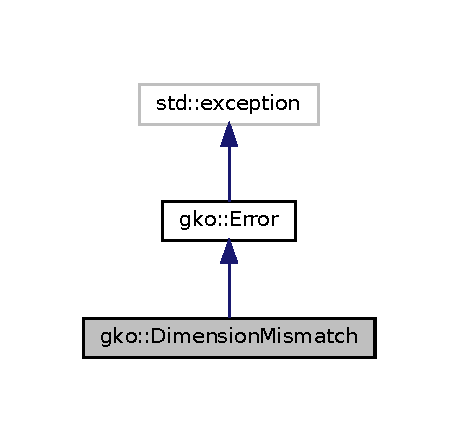
\includegraphics[width=220pt]{classgko_1_1DimensionMismatch__coll__graph}
\end{center}
\end{figure}
\doxysubsection*{Public Member Functions}
\begin{DoxyCompactItemize}
\item 
\mbox{\hyperlink{classgko_1_1DimensionMismatch_ae9ece719cbd41a39835655ba3e70aa47}{Dimension\+Mismatch}} (const std\+::string \&file, int line, const std\+::string \&func, const std\+::string \&first\+\_\+name, \mbox{\hyperlink{namespacegko_a6e5c95df0ae4e47aab2f604a22d98ee7}{size\+\_\+type}} first\+\_\+rows, \mbox{\hyperlink{namespacegko_a6e5c95df0ae4e47aab2f604a22d98ee7}{size\+\_\+type}} first\+\_\+cols, const std\+::string \&second\+\_\+name, \mbox{\hyperlink{namespacegko_a6e5c95df0ae4e47aab2f604a22d98ee7}{size\+\_\+type}} second\+\_\+rows, \mbox{\hyperlink{namespacegko_a6e5c95df0ae4e47aab2f604a22d98ee7}{size\+\_\+type}} second\+\_\+cols, const std\+::string \&clarification)
\begin{DoxyCompactList}\small\item\em Initializes a dimension mismatch error. \end{DoxyCompactList}\end{DoxyCompactItemize}


\doxysubsection{Detailed Description}
\mbox{\hyperlink{classgko_1_1DimensionMismatch}{Dimension\+Mismatch}} is thrown if an operation is being applied to Lin\+Ops of incompatible size. 

\doxysubsection{Constructor \& Destructor Documentation}
\mbox{\Hypertarget{classgko_1_1DimensionMismatch_ae9ece719cbd41a39835655ba3e70aa47}\label{classgko_1_1DimensionMismatch_ae9ece719cbd41a39835655ba3e70aa47}} 
\index{gko::DimensionMismatch@{gko::DimensionMismatch}!DimensionMismatch@{DimensionMismatch}}
\index{DimensionMismatch@{DimensionMismatch}!gko::DimensionMismatch@{gko::DimensionMismatch}}
\doxysubsubsection{\texorpdfstring{DimensionMismatch()}{DimensionMismatch()}}
{\footnotesize\ttfamily gko\+::\+Dimension\+Mismatch\+::\+Dimension\+Mismatch (\begin{DoxyParamCaption}\item[{const std\+::string \&}]{file,  }\item[{int}]{line,  }\item[{const std\+::string \&}]{func,  }\item[{const std\+::string \&}]{first\+\_\+name,  }\item[{\mbox{\hyperlink{namespacegko_a6e5c95df0ae4e47aab2f604a22d98ee7}{size\+\_\+type}}}]{first\+\_\+rows,  }\item[{\mbox{\hyperlink{namespacegko_a6e5c95df0ae4e47aab2f604a22d98ee7}{size\+\_\+type}}}]{first\+\_\+cols,  }\item[{const std\+::string \&}]{second\+\_\+name,  }\item[{\mbox{\hyperlink{namespacegko_a6e5c95df0ae4e47aab2f604a22d98ee7}{size\+\_\+type}}}]{second\+\_\+rows,  }\item[{\mbox{\hyperlink{namespacegko_a6e5c95df0ae4e47aab2f604a22d98ee7}{size\+\_\+type}}}]{second\+\_\+cols,  }\item[{const std\+::string \&}]{clarification }\end{DoxyParamCaption})\hspace{0.3cm}{\ttfamily [inline]}}



Initializes a dimension mismatch error. 


\begin{DoxyParams}{Parameters}
{\em file} & The name of the offending source file \\
\hline
{\em line} & The source code line number where the error occurred \\
\hline
{\em func} & The function name where the error occurred \\
\hline
{\em first\+\_\+name} & The name of the first operator \\
\hline
{\em first\+\_\+rows} & The output dimension of the first operator \\
\hline
{\em first\+\_\+cols} & The input dimension of the first operator \\
\hline
{\em second\+\_\+name} & The name of the second operator \\
\hline
{\em second\+\_\+rows} & The output dimension of the second operator \\
\hline
{\em second\+\_\+cols} & The input dimension of the second operator \\
\hline
{\em clarification} & An additional message describing the error further \\
\hline
\end{DoxyParams}


The documentation for this class was generated from the following file\+:\begin{DoxyCompactItemize}
\item 
ginkgo/core/base/exception.\+hpp (3d7f229d4)\end{DoxyCompactItemize}

\hypertarget{structgko_1_1accessor_1_1div}{}\section{gko\+:\+:accessor\+:\+:div$<$ Kind, First\+Operand, Second\+Operand $>$ Struct Template Reference}
\label{structgko_1_1accessor_1_1div}\index{gko\+::accessor\+::div$<$ Kind, First\+Operand, Second\+Operand $>$@{gko\+::accessor\+::div$<$ Kind, First\+Operand, Second\+Operand $>$}}


Collaboration diagram for gko\+:\+:accessor\+:\+:div$<$ Kind, First\+Operand, Second\+Operand $>$\+:
\nopagebreak
\begin{figure}[H]
\begin{center}
\leavevmode
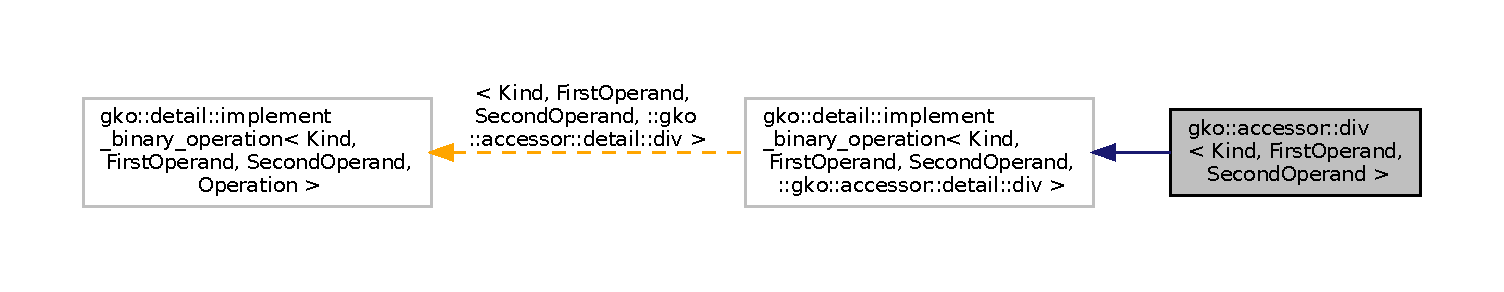
\includegraphics[width=350pt]{structgko_1_1accessor_1_1div__coll__graph}
\end{center}
\end{figure}


The documentation for this struct was generated from the following file\+:\begin{DoxyCompactItemize}
\item 
ginkgo/core/base/range.\+hpp (c828dca0)\end{DoxyCompactItemize}

\hypertarget{classgko_1_1matrix_1_1Ell}{}\doxysection{gko\+::matrix\+::Ell$<$ Value\+Type, Index\+Type $>$ Class Template Reference}
\label{classgko_1_1matrix_1_1Ell}\index{gko::matrix::Ell$<$ ValueType, IndexType $>$@{gko::matrix::Ell$<$ ValueType, IndexType $>$}}


E\+LL is a matrix format where stride with explicit zeros is used such that all rows have the same number of stored elements.  




{\ttfamily \#include $<$ginkgo/core/matrix/ell.\+hpp$>$}



Collaboration diagram for gko\+::matrix\+::Ell$<$ Value\+Type, Index\+Type $>$\+:
\nopagebreak
\begin{figure}[H]
\begin{center}
\leavevmode
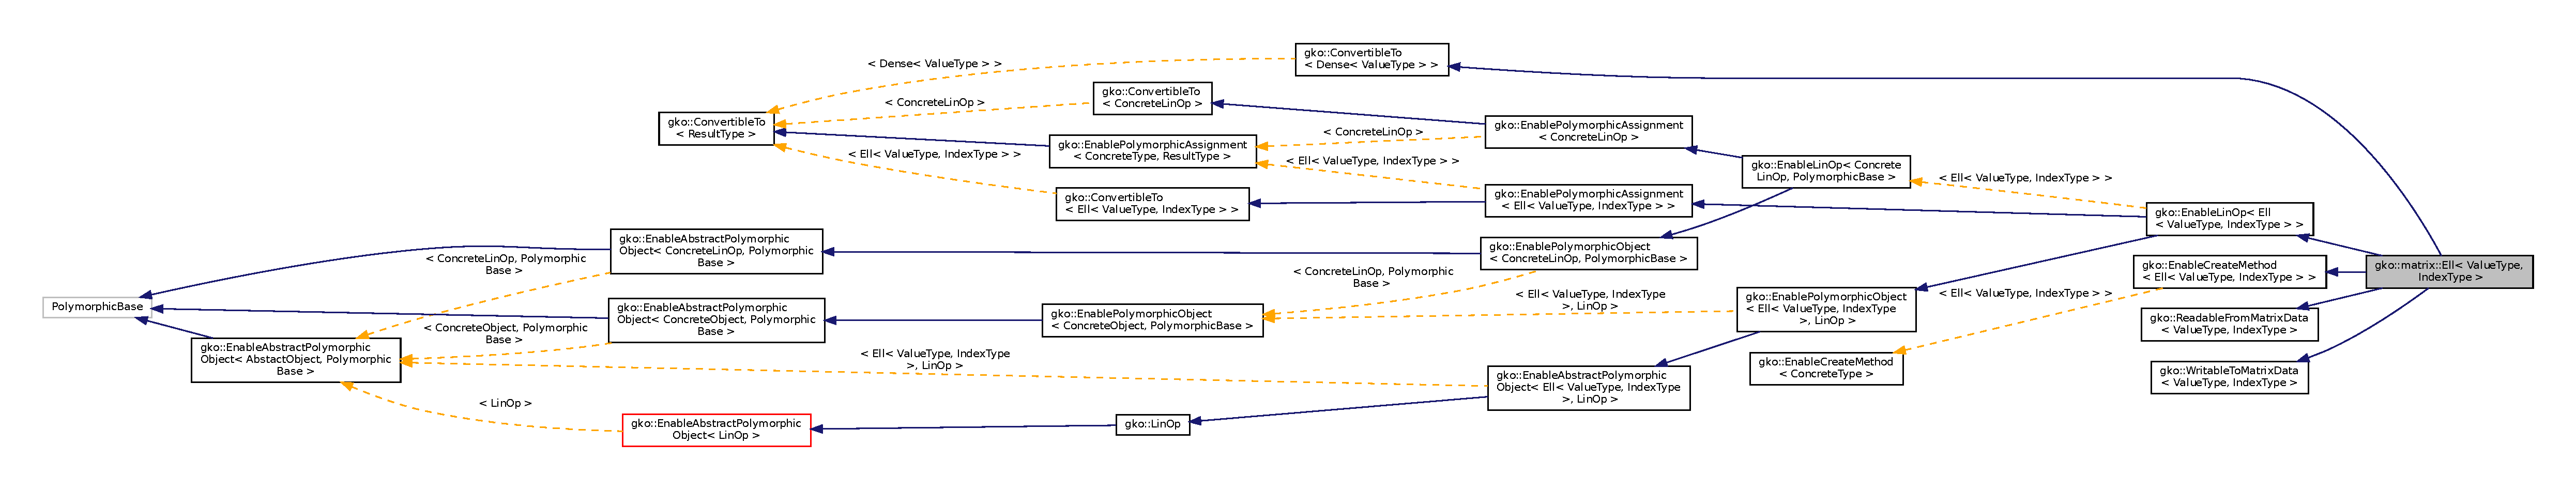
\includegraphics[width=350pt]{classgko_1_1matrix_1_1Ell__coll__graph}
\end{center}
\end{figure}
\doxysubsection*{Public Types}
\begin{DoxyCompactItemize}
\item 
\mbox{\Hypertarget{classgko_1_1matrix_1_1Ell_ae56802e0bd9f47e3d0029b6fdb37db6e}\label{classgko_1_1matrix_1_1Ell_ae56802e0bd9f47e3d0029b6fdb37db6e}} 
using {\bfseries value\+\_\+type} = Value\+Type
\item 
\mbox{\Hypertarget{classgko_1_1matrix_1_1Ell_a17e4809eeab4d76c2887d57e9b4b3cc4}\label{classgko_1_1matrix_1_1Ell_a17e4809eeab4d76c2887d57e9b4b3cc4}} 
using {\bfseries index\+\_\+type} = Index\+Type
\item 
\mbox{\Hypertarget{classgko_1_1matrix_1_1Ell_a993ff3d650fa2f2c72777b856531163a}\label{classgko_1_1matrix_1_1Ell_a993ff3d650fa2f2c72777b856531163a}} 
using {\bfseries mat\+\_\+data} = \mbox{\hyperlink{structgko_1_1matrix__data}{matrix\+\_\+data}}$<$ Value\+Type, Index\+Type $>$
\end{DoxyCompactItemize}
\doxysubsection*{Public Member Functions}
\begin{DoxyCompactItemize}
\item 
\mbox{\Hypertarget{classgko_1_1matrix_1_1Ell_a27157e1cd5530327dc45c3f4162c7328}\label{classgko_1_1matrix_1_1Ell_a27157e1cd5530327dc45c3f4162c7328}} 
void {\bfseries convert\+\_\+to} (\mbox{\hyperlink{classgko_1_1matrix_1_1Ell}{Ell}}$<$ \mbox{\hyperlink{namespacegko_a6362f751c7753cf4fa0a4771d56e8ede}{next\+\_\+precision}}$<$ Value\+Type $>$, Index\+Type $>$ $\ast$result) const override
\item 
\mbox{\Hypertarget{classgko_1_1matrix_1_1Ell_a7a3f5a0133c4b3736bec99f90844e328}\label{classgko_1_1matrix_1_1Ell_a7a3f5a0133c4b3736bec99f90844e328}} 
void {\bfseries move\+\_\+to} (\mbox{\hyperlink{classgko_1_1matrix_1_1Ell}{Ell}}$<$ \mbox{\hyperlink{namespacegko_a6362f751c7753cf4fa0a4771d56e8ede}{next\+\_\+precision}}$<$ Value\+Type $>$, Index\+Type $>$ $\ast$result) override
\item 
\mbox{\Hypertarget{classgko_1_1matrix_1_1Ell_ac7ffdfa4fa0b75b47f49a1373995c1c8}\label{classgko_1_1matrix_1_1Ell_ac7ffdfa4fa0b75b47f49a1373995c1c8}} 
void {\bfseries convert\+\_\+to} (\mbox{\hyperlink{classgko_1_1matrix_1_1Dense}{Dense}}$<$ Value\+Type $>$ $\ast$other) const override
\item 
\mbox{\Hypertarget{classgko_1_1matrix_1_1Ell_aafff71fa45b090208cb6fa29ba495d37}\label{classgko_1_1matrix_1_1Ell_aafff71fa45b090208cb6fa29ba495d37}} 
void {\bfseries move\+\_\+to} (\mbox{\hyperlink{classgko_1_1matrix_1_1Dense}{Dense}}$<$ Value\+Type $>$ $\ast$other) override
\item 
\mbox{\Hypertarget{classgko_1_1matrix_1_1Ell_aa54a287350e098bd1e5f3b243c2ad0d9}\label{classgko_1_1matrix_1_1Ell_aa54a287350e098bd1e5f3b243c2ad0d9}} 
void {\bfseries convert\+\_\+to} (\mbox{\hyperlink{classgko_1_1matrix_1_1Csr}{Csr}}$<$ Value\+Type, Index\+Type $>$ $\ast$other) const override
\item 
\mbox{\Hypertarget{classgko_1_1matrix_1_1Ell_a5d2394c6dfe5568e6e82ab84fc779c40}\label{classgko_1_1matrix_1_1Ell_a5d2394c6dfe5568e6e82ab84fc779c40}} 
void {\bfseries move\+\_\+to} (\mbox{\hyperlink{classgko_1_1matrix_1_1Csr}{Csr}}$<$ Value\+Type, Index\+Type $>$ $\ast$other) override
\item 
void \mbox{\hyperlink{classgko_1_1matrix_1_1Ell_a2c877d9f7bbc57f97df5ab443954a6fd}{read}} (const \mbox{\hyperlink{structgko_1_1matrix__data}{mat\+\_\+data}} \&data) override
\begin{DoxyCompactList}\small\item\em Reads a matrix from a \mbox{\hyperlink{structgko_1_1matrix__data}{matrix\+\_\+data}} structure. \end{DoxyCompactList}\item 
void \mbox{\hyperlink{classgko_1_1matrix_1_1Ell_afa9148a16a9255003055d8e9156ee941}{write}} (\mbox{\hyperlink{structgko_1_1matrix__data}{mat\+\_\+data}} \&data) const override
\begin{DoxyCompactList}\small\item\em Writes a matrix to a \mbox{\hyperlink{structgko_1_1matrix__data}{matrix\+\_\+data}} structure. \end{DoxyCompactList}\item 
value\+\_\+type $\ast$ \mbox{\hyperlink{classgko_1_1matrix_1_1Ell_a4028e9629a7d96a7a483e6ea4a686a1d}{get\+\_\+values}} () noexcept
\begin{DoxyCompactList}\small\item\em Returns the values of the matrix. \end{DoxyCompactList}\item 
const value\+\_\+type $\ast$ \mbox{\hyperlink{classgko_1_1matrix_1_1Ell_a5bc4d3c67b328b353409e76eb9f70803}{get\+\_\+const\+\_\+values}} () const noexcept
\begin{DoxyCompactList}\small\item\em Returns the values of the matrix. \end{DoxyCompactList}\item 
index\+\_\+type $\ast$ \mbox{\hyperlink{classgko_1_1matrix_1_1Ell_ac80ca9482997e97d88425214fd1b8aef}{get\+\_\+col\+\_\+idxs}} () noexcept
\begin{DoxyCompactList}\small\item\em Returns the column indexes of the matrix. \end{DoxyCompactList}\item 
const index\+\_\+type $\ast$ \mbox{\hyperlink{classgko_1_1matrix_1_1Ell_addb3c84f52b090c75f519833fb379cef}{get\+\_\+const\+\_\+col\+\_\+idxs}} () const noexcept
\begin{DoxyCompactList}\small\item\em Returns the column indexes of the matrix. \end{DoxyCompactList}\item 
\mbox{\hyperlink{namespacegko_a6e5c95df0ae4e47aab2f604a22d98ee7}{size\+\_\+type}} \mbox{\hyperlink{classgko_1_1matrix_1_1Ell_a08f9b04b356e58ab57d03ce335ff11ce}{get\+\_\+num\+\_\+stored\+\_\+elements\+\_\+per\+\_\+row}} () const noexcept
\begin{DoxyCompactList}\small\item\em Returns the number of stored elements per row. \end{DoxyCompactList}\item 
\mbox{\hyperlink{namespacegko_a6e5c95df0ae4e47aab2f604a22d98ee7}{size\+\_\+type}} \mbox{\hyperlink{classgko_1_1matrix_1_1Ell_a0be6e75dcea0975b10e3389a9eedacc1}{get\+\_\+stride}} () const noexcept
\begin{DoxyCompactList}\small\item\em Returns the stride of the matrix. \end{DoxyCompactList}\item 
\mbox{\hyperlink{namespacegko_a6e5c95df0ae4e47aab2f604a22d98ee7}{size\+\_\+type}} \mbox{\hyperlink{classgko_1_1matrix_1_1Ell_aecca4e9cfb1e81958881c6dc3e2aa06f}{get\+\_\+num\+\_\+stored\+\_\+elements}} () const noexcept
\begin{DoxyCompactList}\small\item\em Returns the number of elements explicitly stored in the matrix. \end{DoxyCompactList}\item 
value\+\_\+type \& \mbox{\hyperlink{classgko_1_1matrix_1_1Ell_a0d2365837e44dc1889fc16000ff3b0a9}{val\+\_\+at}} (\mbox{\hyperlink{namespacegko_a6e5c95df0ae4e47aab2f604a22d98ee7}{size\+\_\+type}} row, \mbox{\hyperlink{namespacegko_a6e5c95df0ae4e47aab2f604a22d98ee7}{size\+\_\+type}} idx) noexcept
\begin{DoxyCompactList}\small\item\em Returns the {\ttfamily idx}-\/th non-\/zero element of the {\ttfamily row}-\/th row . \end{DoxyCompactList}\item 
value\+\_\+type \mbox{\hyperlink{classgko_1_1matrix_1_1Ell_a3591fa0ab2ec09b43a15b0f0649d8ea3}{val\+\_\+at}} (\mbox{\hyperlink{namespacegko_a6e5c95df0ae4e47aab2f604a22d98ee7}{size\+\_\+type}} row, \mbox{\hyperlink{namespacegko_a6e5c95df0ae4e47aab2f604a22d98ee7}{size\+\_\+type}} idx) const noexcept
\begin{DoxyCompactList}\small\item\em Returns the {\ttfamily idx}-\/th non-\/zero element of the {\ttfamily row}-\/th row . \end{DoxyCompactList}\item 
index\+\_\+type \& \mbox{\hyperlink{classgko_1_1matrix_1_1Ell_a1ef17227a6de85a1c12ebc106abbfc32}{col\+\_\+at}} (\mbox{\hyperlink{namespacegko_a6e5c95df0ae4e47aab2f604a22d98ee7}{size\+\_\+type}} row, \mbox{\hyperlink{namespacegko_a6e5c95df0ae4e47aab2f604a22d98ee7}{size\+\_\+type}} idx) noexcept
\begin{DoxyCompactList}\small\item\em Returns the {\ttfamily idx}-\/th column index of the {\ttfamily row}-\/th row . \end{DoxyCompactList}\item 
index\+\_\+type \mbox{\hyperlink{classgko_1_1matrix_1_1Ell_a1ac1702011ead4e56857de130b4a5301}{col\+\_\+at}} (\mbox{\hyperlink{namespacegko_a6e5c95df0ae4e47aab2f604a22d98ee7}{size\+\_\+type}} row, \mbox{\hyperlink{namespacegko_a6e5c95df0ae4e47aab2f604a22d98ee7}{size\+\_\+type}} idx) const noexcept
\begin{DoxyCompactList}\small\item\em Returns the {\ttfamily idx}-\/th column index of the {\ttfamily row}-\/th row . \end{DoxyCompactList}\end{DoxyCompactItemize}
\doxysubsection*{Friends}
\begin{DoxyCompactItemize}
\item 
\mbox{\Hypertarget{classgko_1_1matrix_1_1Ell_aff1f69cf59ce70d0ad4ccd5fc854c616}\label{classgko_1_1matrix_1_1Ell_aff1f69cf59ce70d0ad4ccd5fc854c616}} 
class {\bfseries Enable\+Create\+Method$<$ Ell $>$}
\item 
\mbox{\Hypertarget{classgko_1_1matrix_1_1Ell_a71537fa3276ed9af486b2167b456f511}\label{classgko_1_1matrix_1_1Ell_a71537fa3276ed9af486b2167b456f511}} 
class {\bfseries Enable\+Polymorphic\+Object$<$ Ell, Lin\+Op $>$}
\item 
\mbox{\Hypertarget{classgko_1_1matrix_1_1Ell_a22a84c8f67f946aa60a2fa8bf5835a32}\label{classgko_1_1matrix_1_1Ell_a22a84c8f67f946aa60a2fa8bf5835a32}} 
class {\bfseries Dense$<$ Value\+Type $>$}
\item 
\mbox{\Hypertarget{classgko_1_1matrix_1_1Ell_a3962faf971a3df6ff4c9226c61fb24cc}\label{classgko_1_1matrix_1_1Ell_a3962faf971a3df6ff4c9226c61fb24cc}} 
class {\bfseries Csr$<$ Value\+Type, Index\+Type $>$}
\item 
\mbox{\Hypertarget{classgko_1_1matrix_1_1Ell_a89acd0bfc3d7c2054773d8e306a60ced}\label{classgko_1_1matrix_1_1Ell_a89acd0bfc3d7c2054773d8e306a60ced}} 
class {\bfseries Ell$<$ next\+\_\+precision$<$ Value\+Type $>$, Index\+Type $>$}
\end{DoxyCompactItemize}
\doxysubsection*{Additional Inherited Members}


\doxysubsection{Detailed Description}
\subsubsection*{template$<$typename Value\+Type = default\+\_\+precision, typename Index\+Type = int32$>$\newline
class gko\+::matrix\+::\+Ell$<$ Value\+Type, Index\+Type $>$}

E\+LL is a matrix format where stride with explicit zeros is used such that all rows have the same number of stored elements. 

The number of elements stored in each row is the largest number of nonzero elements in any of the rows (obtainable through \mbox{\hyperlink{classgko_1_1matrix_1_1Ell_a08f9b04b356e58ab57d03ce335ff11ce}{get\+\_\+num\+\_\+stored\+\_\+elements\+\_\+per\+\_\+row()}} method). This removes the need of a row pointer like in the C\+SR format, and allows for S\+I\+MD processing of the distinct rows. For efficient processing, the nonzero elements and the corresponding column indices are stored in column-\/major fashion. The columns are padded to the length by user-\/defined stride parameter whose default value is the number of rows of the matrix.


\begin{DoxyTemplParams}{Template Parameters}
{\em Value\+Type} & precision of matrix elements \\
\hline
{\em Index\+Type} & precision of matrix indexes \\
\hline
\end{DoxyTemplParams}


\doxysubsection{Member Function Documentation}
\mbox{\Hypertarget{classgko_1_1matrix_1_1Ell_a1ac1702011ead4e56857de130b4a5301}\label{classgko_1_1matrix_1_1Ell_a1ac1702011ead4e56857de130b4a5301}} 
\index{gko::matrix::Ell$<$ ValueType, IndexType $>$@{gko::matrix::Ell$<$ ValueType, IndexType $>$}!col\_at@{col\_at}}
\index{col\_at@{col\_at}!gko::matrix::Ell$<$ ValueType, IndexType $>$@{gko::matrix::Ell$<$ ValueType, IndexType $>$}}
\doxysubsubsection{\texorpdfstring{col\_at()}{col\_at()}\hspace{0.1cm}{\footnotesize\ttfamily [1/2]}}
{\footnotesize\ttfamily template$<$typename Value\+Type = default\+\_\+precision, typename Index\+Type = int32$>$ \\
index\+\_\+type \mbox{\hyperlink{classgko_1_1matrix_1_1Ell}{gko\+::matrix\+::\+Ell}}$<$ Value\+Type, Index\+Type $>$\+::col\+\_\+at (\begin{DoxyParamCaption}\item[{\mbox{\hyperlink{namespacegko_a6e5c95df0ae4e47aab2f604a22d98ee7}{size\+\_\+type}}}]{row,  }\item[{\mbox{\hyperlink{namespacegko_a6e5c95df0ae4e47aab2f604a22d98ee7}{size\+\_\+type}}}]{idx }\end{DoxyParamCaption}) const\hspace{0.3cm}{\ttfamily [inline]}, {\ttfamily [noexcept]}}



Returns the {\ttfamily idx}-\/th column index of the {\ttfamily row}-\/th row . 


\begin{DoxyParams}{Parameters}
{\em row} & the row of the requested element \\
\hline
{\em idx} & the idx-\/th stored element of the row\\
\hline
\end{DoxyParams}
\begin{DoxyNote}{Note}
the method has to be called on the same \mbox{\hyperlink{classgko_1_1Executor}{Executor}} the matrix is stored at (e.\+g. trying to call this method on a G\+PU matrix from the O\+MP results in a runtime error) 
\end{DoxyNote}


References gko\+::matrix\+::\+Ell$<$ Value\+Type, Index\+Type $>$\+::get\+\_\+const\+\_\+col\+\_\+idxs().

\mbox{\Hypertarget{classgko_1_1matrix_1_1Ell_a1ef17227a6de85a1c12ebc106abbfc32}\label{classgko_1_1matrix_1_1Ell_a1ef17227a6de85a1c12ebc106abbfc32}} 
\index{gko::matrix::Ell$<$ ValueType, IndexType $>$@{gko::matrix::Ell$<$ ValueType, IndexType $>$}!col\_at@{col\_at}}
\index{col\_at@{col\_at}!gko::matrix::Ell$<$ ValueType, IndexType $>$@{gko::matrix::Ell$<$ ValueType, IndexType $>$}}
\doxysubsubsection{\texorpdfstring{col\_at()}{col\_at()}\hspace{0.1cm}{\footnotesize\ttfamily [2/2]}}
{\footnotesize\ttfamily template$<$typename Value\+Type = default\+\_\+precision, typename Index\+Type = int32$>$ \\
index\+\_\+type\& \mbox{\hyperlink{classgko_1_1matrix_1_1Ell}{gko\+::matrix\+::\+Ell}}$<$ Value\+Type, Index\+Type $>$\+::col\+\_\+at (\begin{DoxyParamCaption}\item[{\mbox{\hyperlink{namespacegko_a6e5c95df0ae4e47aab2f604a22d98ee7}{size\+\_\+type}}}]{row,  }\item[{\mbox{\hyperlink{namespacegko_a6e5c95df0ae4e47aab2f604a22d98ee7}{size\+\_\+type}}}]{idx }\end{DoxyParamCaption})\hspace{0.3cm}{\ttfamily [inline]}, {\ttfamily [noexcept]}}



Returns the {\ttfamily idx}-\/th column index of the {\ttfamily row}-\/th row . 


\begin{DoxyParams}{Parameters}
{\em row} & the row of the requested element \\
\hline
{\em idx} & the idx-\/th stored element of the row\\
\hline
\end{DoxyParams}
\begin{DoxyNote}{Note}
the method has to be called on the same \mbox{\hyperlink{classgko_1_1Executor}{Executor}} the matrix is stored at (e.\+g. trying to call this method on a G\+PU matrix from the O\+MP results in a runtime error) 
\end{DoxyNote}


References gko\+::matrix\+::\+Ell$<$ Value\+Type, Index\+Type $>$\+::get\+\_\+col\+\_\+idxs().

\mbox{\Hypertarget{classgko_1_1matrix_1_1Ell_ac80ca9482997e97d88425214fd1b8aef}\label{classgko_1_1matrix_1_1Ell_ac80ca9482997e97d88425214fd1b8aef}} 
\index{gko::matrix::Ell$<$ ValueType, IndexType $>$@{gko::matrix::Ell$<$ ValueType, IndexType $>$}!get\_col\_idxs@{get\_col\_idxs}}
\index{get\_col\_idxs@{get\_col\_idxs}!gko::matrix::Ell$<$ ValueType, IndexType $>$@{gko::matrix::Ell$<$ ValueType, IndexType $>$}}
\doxysubsubsection{\texorpdfstring{get\_col\_idxs()}{get\_col\_idxs()}}
{\footnotesize\ttfamily template$<$typename Value\+Type = default\+\_\+precision, typename Index\+Type = int32$>$ \\
index\+\_\+type$\ast$ \mbox{\hyperlink{classgko_1_1matrix_1_1Ell}{gko\+::matrix\+::\+Ell}}$<$ Value\+Type, Index\+Type $>$\+::get\+\_\+col\+\_\+idxs (\begin{DoxyParamCaption}{ }\end{DoxyParamCaption})\hspace{0.3cm}{\ttfamily [inline]}, {\ttfamily [noexcept]}}



Returns the column indexes of the matrix. 

\begin{DoxyReturn}{Returns}
the column indexes of the matrix. 
\end{DoxyReturn}


References gko\+::\+Array$<$ Value\+Type $>$\+::get\+\_\+data().



Referenced by gko\+::matrix\+::\+Ell$<$ Value\+Type, Index\+Type $>$\+::col\+\_\+at().

\mbox{\Hypertarget{classgko_1_1matrix_1_1Ell_addb3c84f52b090c75f519833fb379cef}\label{classgko_1_1matrix_1_1Ell_addb3c84f52b090c75f519833fb379cef}} 
\index{gko::matrix::Ell$<$ ValueType, IndexType $>$@{gko::matrix::Ell$<$ ValueType, IndexType $>$}!get\_const\_col\_idxs@{get\_const\_col\_idxs}}
\index{get\_const\_col\_idxs@{get\_const\_col\_idxs}!gko::matrix::Ell$<$ ValueType, IndexType $>$@{gko::matrix::Ell$<$ ValueType, IndexType $>$}}
\doxysubsubsection{\texorpdfstring{get\_const\_col\_idxs()}{get\_const\_col\_idxs()}}
{\footnotesize\ttfamily template$<$typename Value\+Type = default\+\_\+precision, typename Index\+Type = int32$>$ \\
const index\+\_\+type$\ast$ \mbox{\hyperlink{classgko_1_1matrix_1_1Ell}{gko\+::matrix\+::\+Ell}}$<$ Value\+Type, Index\+Type $>$\+::get\+\_\+const\+\_\+col\+\_\+idxs (\begin{DoxyParamCaption}{ }\end{DoxyParamCaption}) const\hspace{0.3cm}{\ttfamily [inline]}, {\ttfamily [noexcept]}}



Returns the column indexes of the matrix. 

\begin{DoxyReturn}{Returns}
the column indexes of the matrix.
\end{DoxyReturn}
\begin{DoxyNote}{Note}
This is the constant version of the function, which can be significantly more memory efficient than the non-\/constant version, so always prefer this version. 
\end{DoxyNote}


References gko\+::\+Array$<$ Value\+Type $>$\+::get\+\_\+const\+\_\+data().



Referenced by gko\+::matrix\+::\+Ell$<$ Value\+Type, Index\+Type $>$\+::col\+\_\+at().

\mbox{\Hypertarget{classgko_1_1matrix_1_1Ell_a5bc4d3c67b328b353409e76eb9f70803}\label{classgko_1_1matrix_1_1Ell_a5bc4d3c67b328b353409e76eb9f70803}} 
\index{gko::matrix::Ell$<$ ValueType, IndexType $>$@{gko::matrix::Ell$<$ ValueType, IndexType $>$}!get\_const\_values@{get\_const\_values}}
\index{get\_const\_values@{get\_const\_values}!gko::matrix::Ell$<$ ValueType, IndexType $>$@{gko::matrix::Ell$<$ ValueType, IndexType $>$}}
\doxysubsubsection{\texorpdfstring{get\_const\_values()}{get\_const\_values()}}
{\footnotesize\ttfamily template$<$typename Value\+Type = default\+\_\+precision, typename Index\+Type = int32$>$ \\
const value\+\_\+type$\ast$ \mbox{\hyperlink{classgko_1_1matrix_1_1Ell}{gko\+::matrix\+::\+Ell}}$<$ Value\+Type, Index\+Type $>$\+::get\+\_\+const\+\_\+values (\begin{DoxyParamCaption}{ }\end{DoxyParamCaption}) const\hspace{0.3cm}{\ttfamily [inline]}, {\ttfamily [noexcept]}}



Returns the values of the matrix. 

\begin{DoxyReturn}{Returns}
the values of the matrix.
\end{DoxyReturn}
\begin{DoxyNote}{Note}
This is the constant version of the function, which can be significantly more memory efficient than the non-\/constant version, so always prefer this version. 
\end{DoxyNote}


References gko\+::\+Array$<$ Value\+Type $>$\+::get\+\_\+const\+\_\+data().

\mbox{\Hypertarget{classgko_1_1matrix_1_1Ell_aecca4e9cfb1e81958881c6dc3e2aa06f}\label{classgko_1_1matrix_1_1Ell_aecca4e9cfb1e81958881c6dc3e2aa06f}} 
\index{gko::matrix::Ell$<$ ValueType, IndexType $>$@{gko::matrix::Ell$<$ ValueType, IndexType $>$}!get\_num\_stored\_elements@{get\_num\_stored\_elements}}
\index{get\_num\_stored\_elements@{get\_num\_stored\_elements}!gko::matrix::Ell$<$ ValueType, IndexType $>$@{gko::matrix::Ell$<$ ValueType, IndexType $>$}}
\doxysubsubsection{\texorpdfstring{get\_num\_stored\_elements()}{get\_num\_stored\_elements()}}
{\footnotesize\ttfamily template$<$typename Value\+Type = default\+\_\+precision, typename Index\+Type = int32$>$ \\
\mbox{\hyperlink{namespacegko_a6e5c95df0ae4e47aab2f604a22d98ee7}{size\+\_\+type}} \mbox{\hyperlink{classgko_1_1matrix_1_1Ell}{gko\+::matrix\+::\+Ell}}$<$ Value\+Type, Index\+Type $>$\+::get\+\_\+num\+\_\+stored\+\_\+elements (\begin{DoxyParamCaption}{ }\end{DoxyParamCaption}) const\hspace{0.3cm}{\ttfamily [inline]}, {\ttfamily [noexcept]}}



Returns the number of elements explicitly stored in the matrix. 

\begin{DoxyReturn}{Returns}
the number of elements explicitly stored in the matrix 
\end{DoxyReturn}


References gko\+::\+Array$<$ Value\+Type $>$\+::get\+\_\+num\+\_\+elems().

\mbox{\Hypertarget{classgko_1_1matrix_1_1Ell_a08f9b04b356e58ab57d03ce335ff11ce}\label{classgko_1_1matrix_1_1Ell_a08f9b04b356e58ab57d03ce335ff11ce}} 
\index{gko::matrix::Ell$<$ ValueType, IndexType $>$@{gko::matrix::Ell$<$ ValueType, IndexType $>$}!get\_num\_stored\_elements\_per\_row@{get\_num\_stored\_elements\_per\_row}}
\index{get\_num\_stored\_elements\_per\_row@{get\_num\_stored\_elements\_per\_row}!gko::matrix::Ell$<$ ValueType, IndexType $>$@{gko::matrix::Ell$<$ ValueType, IndexType $>$}}
\doxysubsubsection{\texorpdfstring{get\_num\_stored\_elements\_per\_row()}{get\_num\_stored\_elements\_per\_row()}}
{\footnotesize\ttfamily template$<$typename Value\+Type = default\+\_\+precision, typename Index\+Type = int32$>$ \\
\mbox{\hyperlink{namespacegko_a6e5c95df0ae4e47aab2f604a22d98ee7}{size\+\_\+type}} \mbox{\hyperlink{classgko_1_1matrix_1_1Ell}{gko\+::matrix\+::\+Ell}}$<$ Value\+Type, Index\+Type $>$\+::get\+\_\+num\+\_\+stored\+\_\+elements\+\_\+per\+\_\+row (\begin{DoxyParamCaption}{ }\end{DoxyParamCaption}) const\hspace{0.3cm}{\ttfamily [inline]}, {\ttfamily [noexcept]}}



Returns the number of stored elements per row. 

\begin{DoxyReturn}{Returns}
the number of stored elements per row. 
\end{DoxyReturn}
\mbox{\Hypertarget{classgko_1_1matrix_1_1Ell_a0be6e75dcea0975b10e3389a9eedacc1}\label{classgko_1_1matrix_1_1Ell_a0be6e75dcea0975b10e3389a9eedacc1}} 
\index{gko::matrix::Ell$<$ ValueType, IndexType $>$@{gko::matrix::Ell$<$ ValueType, IndexType $>$}!get\_stride@{get\_stride}}
\index{get\_stride@{get\_stride}!gko::matrix::Ell$<$ ValueType, IndexType $>$@{gko::matrix::Ell$<$ ValueType, IndexType $>$}}
\doxysubsubsection{\texorpdfstring{get\_stride()}{get\_stride()}}
{\footnotesize\ttfamily template$<$typename Value\+Type = default\+\_\+precision, typename Index\+Type = int32$>$ \\
\mbox{\hyperlink{namespacegko_a6e5c95df0ae4e47aab2f604a22d98ee7}{size\+\_\+type}} \mbox{\hyperlink{classgko_1_1matrix_1_1Ell}{gko\+::matrix\+::\+Ell}}$<$ Value\+Type, Index\+Type $>$\+::get\+\_\+stride (\begin{DoxyParamCaption}{ }\end{DoxyParamCaption}) const\hspace{0.3cm}{\ttfamily [inline]}, {\ttfamily [noexcept]}}



Returns the stride of the matrix. 

\begin{DoxyReturn}{Returns}
the stride of the matrix. 
\end{DoxyReturn}
\mbox{\Hypertarget{classgko_1_1matrix_1_1Ell_a4028e9629a7d96a7a483e6ea4a686a1d}\label{classgko_1_1matrix_1_1Ell_a4028e9629a7d96a7a483e6ea4a686a1d}} 
\index{gko::matrix::Ell$<$ ValueType, IndexType $>$@{gko::matrix::Ell$<$ ValueType, IndexType $>$}!get\_values@{get\_values}}
\index{get\_values@{get\_values}!gko::matrix::Ell$<$ ValueType, IndexType $>$@{gko::matrix::Ell$<$ ValueType, IndexType $>$}}
\doxysubsubsection{\texorpdfstring{get\_values()}{get\_values()}}
{\footnotesize\ttfamily template$<$typename Value\+Type = default\+\_\+precision, typename Index\+Type = int32$>$ \\
value\+\_\+type$\ast$ \mbox{\hyperlink{classgko_1_1matrix_1_1Ell}{gko\+::matrix\+::\+Ell}}$<$ Value\+Type, Index\+Type $>$\+::get\+\_\+values (\begin{DoxyParamCaption}{ }\end{DoxyParamCaption})\hspace{0.3cm}{\ttfamily [inline]}, {\ttfamily [noexcept]}}



Returns the values of the matrix. 

\begin{DoxyReturn}{Returns}
the values of the matrix. 
\end{DoxyReturn}


References gko\+::\+Array$<$ Value\+Type $>$\+::get\+\_\+data().

\mbox{\Hypertarget{classgko_1_1matrix_1_1Ell_a2c877d9f7bbc57f97df5ab443954a6fd}\label{classgko_1_1matrix_1_1Ell_a2c877d9f7bbc57f97df5ab443954a6fd}} 
\index{gko::matrix::Ell$<$ ValueType, IndexType $>$@{gko::matrix::Ell$<$ ValueType, IndexType $>$}!read@{read}}
\index{read@{read}!gko::matrix::Ell$<$ ValueType, IndexType $>$@{gko::matrix::Ell$<$ ValueType, IndexType $>$}}
\doxysubsubsection{\texorpdfstring{read()}{read()}}
{\footnotesize\ttfamily template$<$typename Value\+Type = default\+\_\+precision, typename Index\+Type = int32$>$ \\
void \mbox{\hyperlink{classgko_1_1matrix_1_1Ell}{gko\+::matrix\+::\+Ell}}$<$ Value\+Type, Index\+Type $>$\+::read (\begin{DoxyParamCaption}\item[{const \mbox{\hyperlink{structgko_1_1matrix__data}{mat\+\_\+data}} \&}]{data }\end{DoxyParamCaption})\hspace{0.3cm}{\ttfamily [override]}, {\ttfamily [virtual]}}



Reads a matrix from a \mbox{\hyperlink{structgko_1_1matrix__data}{matrix\+\_\+data}} structure. 


\begin{DoxyParams}{Parameters}
{\em data} & the \mbox{\hyperlink{structgko_1_1matrix__data}{matrix\+\_\+data}} structure \\
\hline
\end{DoxyParams}


Implements \mbox{\hyperlink{classgko_1_1ReadableFromMatrixData_add5c12e23b3ac3c8fbd607fa5a9656bb}{gko\+::\+Readable\+From\+Matrix\+Data$<$ Value\+Type, Index\+Type $>$}}.

\mbox{\Hypertarget{classgko_1_1matrix_1_1Ell_a3591fa0ab2ec09b43a15b0f0649d8ea3}\label{classgko_1_1matrix_1_1Ell_a3591fa0ab2ec09b43a15b0f0649d8ea3}} 
\index{gko::matrix::Ell$<$ ValueType, IndexType $>$@{gko::matrix::Ell$<$ ValueType, IndexType $>$}!val\_at@{val\_at}}
\index{val\_at@{val\_at}!gko::matrix::Ell$<$ ValueType, IndexType $>$@{gko::matrix::Ell$<$ ValueType, IndexType $>$}}
\doxysubsubsection{\texorpdfstring{val\_at()}{val\_at()}\hspace{0.1cm}{\footnotesize\ttfamily [1/2]}}
{\footnotesize\ttfamily template$<$typename Value\+Type = default\+\_\+precision, typename Index\+Type = int32$>$ \\
value\+\_\+type \mbox{\hyperlink{classgko_1_1matrix_1_1Ell}{gko\+::matrix\+::\+Ell}}$<$ Value\+Type, Index\+Type $>$\+::val\+\_\+at (\begin{DoxyParamCaption}\item[{\mbox{\hyperlink{namespacegko_a6e5c95df0ae4e47aab2f604a22d98ee7}{size\+\_\+type}}}]{row,  }\item[{\mbox{\hyperlink{namespacegko_a6e5c95df0ae4e47aab2f604a22d98ee7}{size\+\_\+type}}}]{idx }\end{DoxyParamCaption}) const\hspace{0.3cm}{\ttfamily [inline]}, {\ttfamily [noexcept]}}



Returns the {\ttfamily idx}-\/th non-\/zero element of the {\ttfamily row}-\/th row . 


\begin{DoxyParams}{Parameters}
{\em row} & the row of the requested element \\
\hline
{\em idx} & the idx-\/th stored element of the row\\
\hline
\end{DoxyParams}
\begin{DoxyNote}{Note}
the method has to be called on the same \mbox{\hyperlink{classgko_1_1Executor}{Executor}} the matrix is stored at (e.\+g. trying to call this method on a G\+PU matrix from the O\+MP results in a runtime error) 
\end{DoxyNote}


References gko\+::\+Array$<$ Value\+Type $>$\+::get\+\_\+const\+\_\+data().

\mbox{\Hypertarget{classgko_1_1matrix_1_1Ell_a0d2365837e44dc1889fc16000ff3b0a9}\label{classgko_1_1matrix_1_1Ell_a0d2365837e44dc1889fc16000ff3b0a9}} 
\index{gko::matrix::Ell$<$ ValueType, IndexType $>$@{gko::matrix::Ell$<$ ValueType, IndexType $>$}!val\_at@{val\_at}}
\index{val\_at@{val\_at}!gko::matrix::Ell$<$ ValueType, IndexType $>$@{gko::matrix::Ell$<$ ValueType, IndexType $>$}}
\doxysubsubsection{\texorpdfstring{val\_at()}{val\_at()}\hspace{0.1cm}{\footnotesize\ttfamily [2/2]}}
{\footnotesize\ttfamily template$<$typename Value\+Type = default\+\_\+precision, typename Index\+Type = int32$>$ \\
value\+\_\+type\& \mbox{\hyperlink{classgko_1_1matrix_1_1Ell}{gko\+::matrix\+::\+Ell}}$<$ Value\+Type, Index\+Type $>$\+::val\+\_\+at (\begin{DoxyParamCaption}\item[{\mbox{\hyperlink{namespacegko_a6e5c95df0ae4e47aab2f604a22d98ee7}{size\+\_\+type}}}]{row,  }\item[{\mbox{\hyperlink{namespacegko_a6e5c95df0ae4e47aab2f604a22d98ee7}{size\+\_\+type}}}]{idx }\end{DoxyParamCaption})\hspace{0.3cm}{\ttfamily [inline]}, {\ttfamily [noexcept]}}



Returns the {\ttfamily idx}-\/th non-\/zero element of the {\ttfamily row}-\/th row . 


\begin{DoxyParams}{Parameters}
{\em row} & the row of the requested element \\
\hline
{\em idx} & the idx-\/th stored element of the row\\
\hline
\end{DoxyParams}
\begin{DoxyNote}{Note}
the method has to be called on the same \mbox{\hyperlink{classgko_1_1Executor}{Executor}} the matrix is stored at (e.\+g. trying to call this method on a G\+PU matrix from the O\+MP results in a runtime error) 
\end{DoxyNote}


References gko\+::\+Array$<$ Value\+Type $>$\+::get\+\_\+data().

\mbox{\Hypertarget{classgko_1_1matrix_1_1Ell_afa9148a16a9255003055d8e9156ee941}\label{classgko_1_1matrix_1_1Ell_afa9148a16a9255003055d8e9156ee941}} 
\index{gko::matrix::Ell$<$ ValueType, IndexType $>$@{gko::matrix::Ell$<$ ValueType, IndexType $>$}!write@{write}}
\index{write@{write}!gko::matrix::Ell$<$ ValueType, IndexType $>$@{gko::matrix::Ell$<$ ValueType, IndexType $>$}}
\doxysubsubsection{\texorpdfstring{write()}{write()}}
{\footnotesize\ttfamily template$<$typename Value\+Type = default\+\_\+precision, typename Index\+Type = int32$>$ \\
void \mbox{\hyperlink{classgko_1_1matrix_1_1Ell}{gko\+::matrix\+::\+Ell}}$<$ Value\+Type, Index\+Type $>$\+::write (\begin{DoxyParamCaption}\item[{\mbox{\hyperlink{structgko_1_1matrix__data}{mat\+\_\+data}} \&}]{data }\end{DoxyParamCaption}) const\hspace{0.3cm}{\ttfamily [override]}, {\ttfamily [virtual]}}



Writes a matrix to a \mbox{\hyperlink{structgko_1_1matrix__data}{matrix\+\_\+data}} structure. 


\begin{DoxyParams}{Parameters}
{\em data} & the \mbox{\hyperlink{structgko_1_1matrix__data}{matrix\+\_\+data}} structure \\
\hline
\end{DoxyParams}


Implements \mbox{\hyperlink{classgko_1_1WritableToMatrixData_a96036c3a4bf4c67fa93002808b8b14e2}{gko\+::\+Writable\+To\+Matrix\+Data$<$ Value\+Type, Index\+Type $>$}}.



The documentation for this class was generated from the following files\+:\begin{DoxyCompactItemize}
\item 
ginkgo/core/matrix/csr.\+hpp (3b11599ff)\item 
ginkgo/core/matrix/ell.\+hpp (8a86dad58)\end{DoxyCompactItemize}

\hypertarget{structgko_1_1enable__parameters__type}{}\section{gko\+:\+:enable\+\_\+parameters\+\_\+type$<$ Concrete\+Parameters\+Type, Factory $>$ Struct Template Reference}
\label{structgko_1_1enable__parameters__type}\index{gko\+::enable\+\_\+parameters\+\_\+type$<$ Concrete\+Parameters\+Type, Factory $>$@{gko\+::enable\+\_\+parameters\+\_\+type$<$ Concrete\+Parameters\+Type, Factory $>$}}


The \hyperlink{structgko_1_1enable__parameters__type}{enable\+\_\+parameters\+\_\+type} mixin is used to create a base implementation of the factory parameters structure.  




{\ttfamily \#include $<$ginkgo/core/base/abstract\+\_\+factory.\+hpp$>$}

\subsection*{Public Types}
\begin{DoxyCompactItemize}
\item 
\mbox{\Hypertarget{structgko_1_1enable__parameters__type_a0d16b999fffe1aecfbc4824381352268}\label{structgko_1_1enable__parameters__type_a0d16b999fffe1aecfbc4824381352268}} 
using {\bfseries factory} = Factory
\end{DoxyCompactItemize}
\subsection*{Public Member Functions}
\begin{DoxyCompactItemize}
\item 
std\+::unique\+\_\+ptr$<$ Factory $>$ \hyperlink{structgko_1_1enable__parameters__type_a07bc1963e83201576761e013f22ce621}{on} (std\+::shared\+\_\+ptr$<$ const \hyperlink{classgko_1_1Executor}{Executor} $>$ exec) const
\begin{DoxyCompactList}\small\item\em Creates a new factory on the specified executor. \end{DoxyCompactList}\end{DoxyCompactItemize}


\subsection{Detailed Description}
\subsubsection*{template$<$typename Concrete\+Parameters\+Type, typename Factory$>$\newline
struct gko\+::enable\+\_\+parameters\+\_\+type$<$ Concrete\+Parameters\+Type, Factory $>$}

The \hyperlink{structgko_1_1enable__parameters__type}{enable\+\_\+parameters\+\_\+type} mixin is used to create a base implementation of the factory parameters structure. 

It provides only the \hyperlink{structgko_1_1enable__parameters__type_a07bc1963e83201576761e013f22ce621}{on()} method which can be used to instantiate the factory give the parameters stored in the structure.


\begin{DoxyTemplParams}{Template Parameters}
{\em Concrete\+Parameters\+Type} & the concrete parameters type which is being implemented \mbox{[}C\+R\+TP parameter\mbox{]} \\
\hline
{\em Factory} & the concrete factory for which these parameters are being used \\
\hline
\end{DoxyTemplParams}


\subsection{Member Function Documentation}
\mbox{\Hypertarget{structgko_1_1enable__parameters__type_a07bc1963e83201576761e013f22ce621}\label{structgko_1_1enable__parameters__type_a07bc1963e83201576761e013f22ce621}} 
\index{gko\+::enable\+\_\+parameters\+\_\+type@{gko\+::enable\+\_\+parameters\+\_\+type}!on@{on}}
\index{on@{on}!gko\+::enable\+\_\+parameters\+\_\+type@{gko\+::enable\+\_\+parameters\+\_\+type}}
\subsubsection{\texorpdfstring{on()}{on()}}
{\footnotesize\ttfamily template$<$typename Concrete\+Parameters\+Type, typename Factory$>$ \\
std\+::unique\+\_\+ptr$<$Factory$>$ \hyperlink{structgko_1_1enable__parameters__type}{gko\+::enable\+\_\+parameters\+\_\+type}$<$ Concrete\+Parameters\+Type, Factory $>$\+::on (\begin{DoxyParamCaption}\item[{std\+::shared\+\_\+ptr$<$ const \hyperlink{classgko_1_1Executor}{Executor} $>$}]{exec }\end{DoxyParamCaption}) const}



Creates a new factory on the specified executor. 


\begin{DoxyParams}{Parameters}
{\em exec} & the executor where the factory will be created\\
\hline
\end{DoxyParams}
\begin{DoxyReturn}{Returns}
a new factory instance 
\end{DoxyReturn}


The documentation for this struct was generated from the following file\+:\begin{DoxyCompactItemize}
\item 
ginkgo/core/base/abstract\+\_\+factory.\+hpp (99beb325)\end{DoxyCompactItemize}

\hypertarget{classgko_1_1EnableAbstractPolymorphicObject}{}\doxysection{gko\+::Enable\+Abstract\+Polymorphic\+Object$<$ Abstact\+Object, Polymorphic\+Base $>$ Class Template Reference}
\label{classgko_1_1EnableAbstractPolymorphicObject}\index{gko::EnableAbstractPolymorphicObject$<$ AbstactObject, PolymorphicBase $>$@{gko::EnableAbstractPolymorphicObject$<$ AbstactObject, PolymorphicBase $>$}}


This mixin inherits from (a subclass of) \mbox{\hyperlink{classgko_1_1PolymorphicObject}{Polymorphic\+Object}} and provides a base implementation of a new abstract object.  




{\ttfamily \#include $<$ginkgo/core/base/polymorphic\+\_\+object.\+hpp$>$}



Collaboration diagram for gko\+::Enable\+Abstract\+Polymorphic\+Object$<$ Abstact\+Object, Polymorphic\+Base $>$\+:
\nopagebreak
\begin{figure}[H]
\begin{center}
\leavevmode
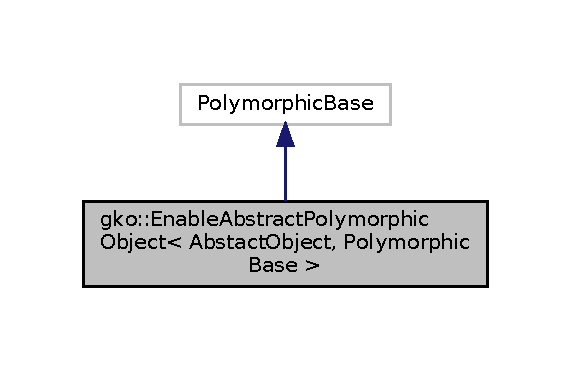
\includegraphics[width=274pt]{classgko_1_1EnableAbstractPolymorphicObject__coll__graph}
\end{center}
\end{figure}
\doxysubsection*{Public Member Functions}
\begin{DoxyCompactItemize}
\item 
\mbox{\Hypertarget{classgko_1_1EnableAbstractPolymorphicObject_afe4ec718648d83a9558d3857814c9b9a}\label{classgko_1_1EnableAbstractPolymorphicObject_afe4ec718648d83a9558d3857814c9b9a}} 
std\+::unique\+\_\+ptr$<$ Abstact\+Object $>$ {\bfseries create\+\_\+default} (std\+::shared\+\_\+ptr$<$ const \mbox{\hyperlink{classgko_1_1Executor}{Executor}} $>$ exec) const
\item 
\mbox{\Hypertarget{classgko_1_1EnableAbstractPolymorphicObject_a26c03af9356362ec0ca4f7b9c4085583}\label{classgko_1_1EnableAbstractPolymorphicObject_a26c03af9356362ec0ca4f7b9c4085583}} 
std\+::unique\+\_\+ptr$<$ Abstact\+Object $>$ {\bfseries create\+\_\+default} () const
\item 
\mbox{\Hypertarget{classgko_1_1EnableAbstractPolymorphicObject_a6183560a0ccc5c8cbc4be2e9ad27c000}\label{classgko_1_1EnableAbstractPolymorphicObject_a6183560a0ccc5c8cbc4be2e9ad27c000}} 
std\+::unique\+\_\+ptr$<$ Abstact\+Object $>$ {\bfseries clone} (std\+::shared\+\_\+ptr$<$ const \mbox{\hyperlink{classgko_1_1Executor}{Executor}} $>$ exec) const
\item 
\mbox{\Hypertarget{classgko_1_1EnableAbstractPolymorphicObject_aff03b057dd81865dbbe09e708b368f36}\label{classgko_1_1EnableAbstractPolymorphicObject_aff03b057dd81865dbbe09e708b368f36}} 
std\+::unique\+\_\+ptr$<$ Abstact\+Object $>$ {\bfseries clone} () const
\item 
\mbox{\Hypertarget{classgko_1_1EnableAbstractPolymorphicObject_a85130926792743e8ae61af1b4beb003c}\label{classgko_1_1EnableAbstractPolymorphicObject_a85130926792743e8ae61af1b4beb003c}} 
Abstact\+Object $\ast$ {\bfseries copy\+\_\+from} (const \mbox{\hyperlink{classgko_1_1PolymorphicObject}{Polymorphic\+Object}} $\ast$other)
\item 
\mbox{\Hypertarget{classgko_1_1EnableAbstractPolymorphicObject_a1c021e3710785503593b7054d8c1210d}\label{classgko_1_1EnableAbstractPolymorphicObject_a1c021e3710785503593b7054d8c1210d}} 
Abstact\+Object $\ast$ {\bfseries copy\+\_\+from} (std\+::unique\+\_\+ptr$<$ \mbox{\hyperlink{classgko_1_1PolymorphicObject}{Polymorphic\+Object}} $>$ other)
\item 
\mbox{\Hypertarget{classgko_1_1EnableAbstractPolymorphicObject_a4f42a63eedf0bc751262d4493651146a}\label{classgko_1_1EnableAbstractPolymorphicObject_a4f42a63eedf0bc751262d4493651146a}} 
Abstact\+Object $\ast$ {\bfseries clear} ()
\end{DoxyCompactItemize}


\doxysubsection{Detailed Description}
\subsubsection*{template$<$typename Abstact\+Object, typename Polymorphic\+Base = Polymorphic\+Object$>$\newline
class gko\+::\+Enable\+Abstract\+Polymorphic\+Object$<$ Abstact\+Object, Polymorphic\+Base $>$}

This mixin inherits from (a subclass of) \mbox{\hyperlink{classgko_1_1PolymorphicObject}{Polymorphic\+Object}} and provides a base implementation of a new abstract object. 

It uses method hiding to update the parameter and return types from {\ttfamily \mbox{\hyperlink{classgko_1_1PolymorphicObject}{Polymorphic\+Object}} to}Abstract\+Object\`{} wherever it makes sense. As opposed to \mbox{\hyperlink{classgko_1_1EnablePolymorphicObject}{Enable\+Polymorphic\+Object}}, it does not implement \mbox{\hyperlink{classgko_1_1PolymorphicObject}{Polymorphic\+Object}}\textquotesingle{}s virtual methods.


\begin{DoxyTemplParams}{Template Parameters}
{\em Abstract\+Object} & the abstract class which is being implemented \mbox{[}C\+R\+TP parameter\mbox{]} \\
\hline
{\em Polymorphic\+Base} & parent of Abstract\+Object in the polymorphic hierarchy, has to be a subclass of polymorphic object\\
\hline
\end{DoxyTemplParams}
\begin{DoxySeeAlso}{See also}
\mbox{\hyperlink{classgko_1_1EnablePolymorphicObject}{Enable\+Polymorphic\+Object}} for creating a concrete subclass of \mbox{\hyperlink{classgko_1_1PolymorphicObject}{Polymorphic\+Object}}. 
\end{DoxySeeAlso}


The documentation for this class was generated from the following file\+:\begin{DoxyCompactItemize}
\item 
ginkgo/core/base/polymorphic\+\_\+object.\+hpp (efd48502f)\end{DoxyCompactItemize}

\hypertarget{classgko_1_1EnableCreateMethod}{}\doxysection{gko\+::Enable\+Create\+Method$<$ Concrete\+Type $>$ Class Template Reference}
\label{classgko_1_1EnableCreateMethod}\index{gko::EnableCreateMethod$<$ ConcreteType $>$@{gko::EnableCreateMethod$<$ ConcreteType $>$}}


This mixin implements a static {\ttfamily create()} method on {\ttfamily Concrete\+Type} that dynamically allocates the memory, uses the passed-\/in arguments to construct the object, and returns an std\+::unique\+\_\+ptr to such an object.  




{\ttfamily \#include $<$ginkgo/core/base/polymorphic\+\_\+object.\+hpp$>$}

\doxysubsection*{Static Public Member Functions}
\begin{DoxyCompactItemize}
\item 
\mbox{\Hypertarget{classgko_1_1EnableCreateMethod_aa732d4d8736a4ade9206b9641cd1edd5}\label{classgko_1_1EnableCreateMethod_aa732d4d8736a4ade9206b9641cd1edd5}} 
{\footnotesize template$<$typename... Args$>$ }\\static std\+::unique\+\_\+ptr$<$ Concrete\+Type $>$ {\bfseries create} (Args \&\&... args)
\end{DoxyCompactItemize}


\doxysubsection{Detailed Description}
\subsubsection*{template$<$typename Concrete\+Type$>$\newline
class gko\+::\+Enable\+Create\+Method$<$ Concrete\+Type $>$}

This mixin implements a static {\ttfamily create()} method on {\ttfamily Concrete\+Type} that dynamically allocates the memory, uses the passed-\/in arguments to construct the object, and returns an std\+::unique\+\_\+ptr to such an object. 


\begin{DoxyTemplParams}{Template Parameters}
{\em Concrete\+Object} & the concrete type for which {\ttfamily create()} is being implemented \mbox{[}C\+R\+TP parameter\mbox{]} \\
\hline
\end{DoxyTemplParams}


The documentation for this class was generated from the following file\+:\begin{DoxyCompactItemize}
\item 
ginkgo/core/base/polymorphic\+\_\+object.\+hpp (3190c3e0f)\end{DoxyCompactItemize}

\hypertarget{classgko_1_1EnableDefaultFactory}{}\doxysection{gko\+::Enable\+Default\+Factory$<$ Concrete\+Factory, Product\+Type, Parameters\+Type, Polymorphic\+Base $>$ Class Template Reference}
\label{classgko_1_1EnableDefaultFactory}\index{gko::EnableDefaultFactory$<$ ConcreteFactory, ProductType, ParametersType, PolymorphicBase $>$@{gko::EnableDefaultFactory$<$ ConcreteFactory, ProductType, ParametersType, PolymorphicBase $>$}}


This mixin provides a default implementation of a concrete factory.  




{\ttfamily \#include $<$ginkgo/core/base/abstract\+\_\+factory.\+hpp$>$}



Collaboration diagram for gko\+::Enable\+Default\+Factory$<$ Concrete\+Factory, Product\+Type, Parameters\+Type, Polymorphic\+Base $>$\+:
\nopagebreak
\begin{figure}[H]
\begin{center}
\leavevmode
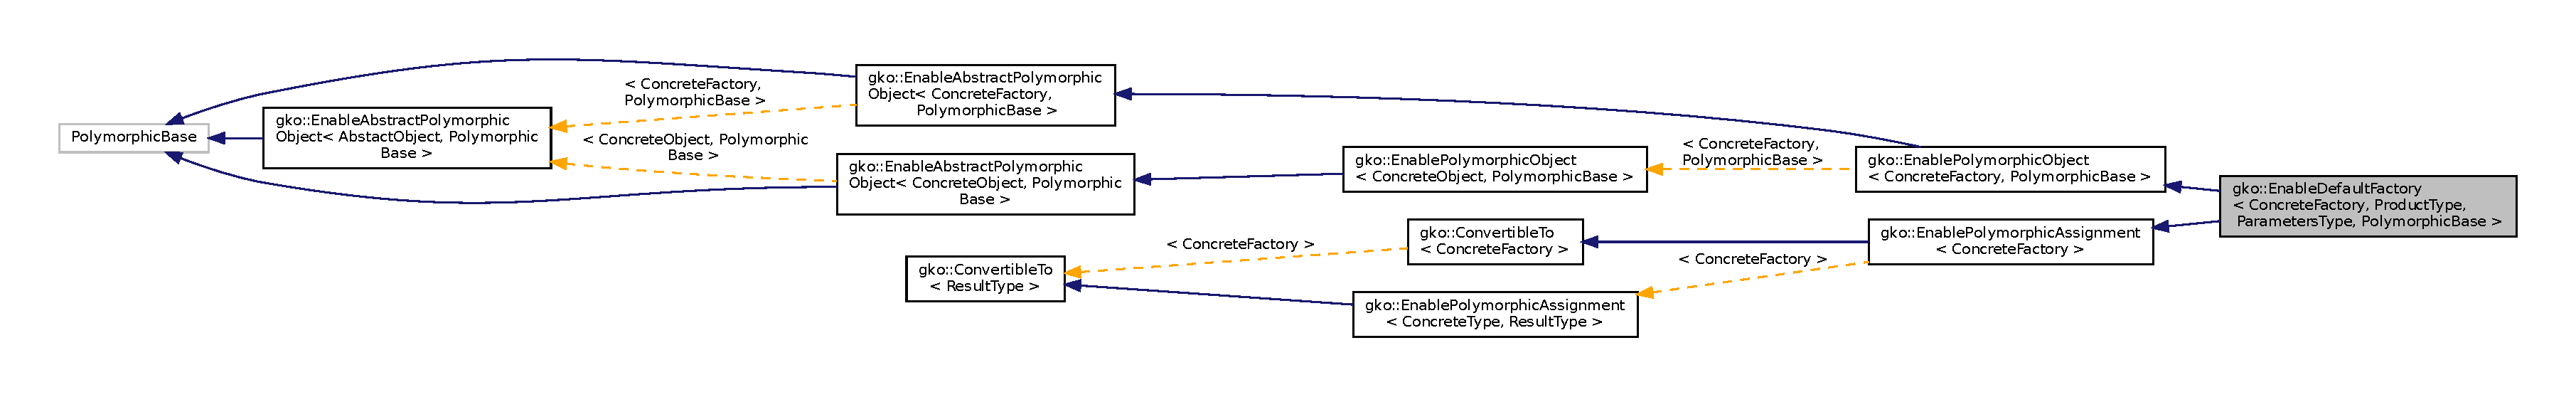
\includegraphics[width=350pt]{classgko_1_1EnableDefaultFactory__coll__graph}
\end{center}
\end{figure}
\doxysubsection*{Public Types}
\begin{DoxyCompactItemize}
\item 
\mbox{\Hypertarget{classgko_1_1EnableDefaultFactory_ac762510ed96961493c273338ca358ecf}\label{classgko_1_1EnableDefaultFactory_ac762510ed96961493c273338ca358ecf}} 
using {\bfseries product\+\_\+type} = Product\+Type
\item 
\mbox{\Hypertarget{classgko_1_1EnableDefaultFactory_a911e420cd7f7c7f5550abbf0e788b59a}\label{classgko_1_1EnableDefaultFactory_a911e420cd7f7c7f5550abbf0e788b59a}} 
using {\bfseries parameters\+\_\+type} = Parameters\+Type
\item 
\mbox{\Hypertarget{classgko_1_1EnableDefaultFactory_a76344d95116ad7c95190152ecd64c2fb}\label{classgko_1_1EnableDefaultFactory_a76344d95116ad7c95190152ecd64c2fb}} 
using {\bfseries polymorphic\+\_\+base} = Polymorphic\+Base
\item 
\mbox{\Hypertarget{classgko_1_1EnableDefaultFactory_ae1741e6f98c9a038a0bae24804a20f34}\label{classgko_1_1EnableDefaultFactory_ae1741e6f98c9a038a0bae24804a20f34}} 
using {\bfseries abstract\+\_\+product\+\_\+type} = typename Polymorphic\+Base\+::abstract\+\_\+product\+\_\+type
\item 
\mbox{\Hypertarget{classgko_1_1EnableDefaultFactory_a5006a049ebb2f4d5c0f274f9d82ce870}\label{classgko_1_1EnableDefaultFactory_a5006a049ebb2f4d5c0f274f9d82ce870}} 
using {\bfseries components\+\_\+type} = typename Polymorphic\+Base\+::components\+\_\+type
\end{DoxyCompactItemize}
\doxysubsection*{Public Member Functions}
\begin{DoxyCompactItemize}
\item 
\mbox{\Hypertarget{classgko_1_1EnableDefaultFactory_adc2fe350c1549e20ff5fec67c315d8f4}\label{classgko_1_1EnableDefaultFactory_adc2fe350c1549e20ff5fec67c315d8f4}} 
{\footnotesize template$<$typename... Args$>$ }\\std\+::unique\+\_\+ptr$<$ Product\+Type $>$ {\bfseries generate} (Args \&\&... args) const
\item 
const parameters\+\_\+type \& \mbox{\hyperlink{classgko_1_1EnableDefaultFactory_ae32f2b3100640293f3a46e1280965162}{get\+\_\+parameters}} () const noexcept
\begin{DoxyCompactList}\small\item\em Returns the parameters of the factory. \end{DoxyCompactList}\end{DoxyCompactItemize}
\doxysubsection*{Static Public Member Functions}
\begin{DoxyCompactItemize}
\item 
static parameters\+\_\+type \mbox{\hyperlink{classgko_1_1EnableDefaultFactory_a1d077101d9e788e6c65f088612d14cc3}{create}} ()
\begin{DoxyCompactList}\small\item\em Creates a new Parameters\+Type object which can be used to instantiate a new Concrete\+Factory. \end{DoxyCompactList}\end{DoxyCompactItemize}
\doxysubsection*{Friends}
\begin{DoxyCompactItemize}
\item 
\mbox{\Hypertarget{classgko_1_1EnableDefaultFactory_a01a6ad051cccd6915df38622922a5bb6}\label{classgko_1_1EnableDefaultFactory_a01a6ad051cccd6915df38622922a5bb6}} 
class {\bfseries Enable\+Polymorphic\+Object$<$ Concrete\+Factory, Polymorphic\+Base $>$}
\end{DoxyCompactItemize}


\doxysubsection{Detailed Description}
\subsubsection*{template$<$typename Concrete\+Factory, typename Product\+Type, typename Parameters\+Type, typename Polymorphic\+Base$>$\newline
class gko\+::\+Enable\+Default\+Factory$<$ Concrete\+Factory, Product\+Type, Parameters\+Type, Polymorphic\+Base $>$}

This mixin provides a default implementation of a concrete factory. 

It implements all the methods of \mbox{\hyperlink{classgko_1_1AbstractFactory}{Abstract\+Factory}} and \mbox{\hyperlink{classgko_1_1PolymorphicObject}{Polymorphic\+Object}}. Its implementation of the generate\+\_\+impl() method delegates the creation of the product by calling the {\ttfamily Product\+Type\+::\+Product\+Type(const Concrete\+Factory $\ast$, const components\+\_\+type \&)} constructor. The factory also supports parameters by using the {\ttfamily Parameters\+Type} structure, which is defined by the user.

For a simple example, see Int\+Factory in {\ttfamily core/test/base/abstract\+\_\+factory.\+cpp}.


\begin{DoxyTemplParams}{Template Parameters}
{\em Concrete\+Factory} & the concrete factory which is being implemented \mbox{[}C\+R\+TP parameter\mbox{]} \\
\hline
{\em Product\+Type} & the concrete type of products which this factory produces, has to be a subclass of Polymorphic\+Base\+::abstract\+\_\+product\+\_\+type \\
\hline
{\em Parameters\+Type} & a type representing the parameters of the factory, has to inherit from the \mbox{\hyperlink{structgko_1_1enable__parameters__type}{enable\+\_\+parameters\+\_\+type}} mixin \\
\hline
{\em Polymorphic\+Base} & parent of Concrete\+Factory in the polymorphic hierarchy, has to be a subclass of \mbox{\hyperlink{classgko_1_1AbstractFactory}{Abstract\+Factory}} \\
\hline
\end{DoxyTemplParams}


\doxysubsection{Member Function Documentation}
\mbox{\Hypertarget{classgko_1_1EnableDefaultFactory_a1d077101d9e788e6c65f088612d14cc3}\label{classgko_1_1EnableDefaultFactory_a1d077101d9e788e6c65f088612d14cc3}} 
\index{gko::EnableDefaultFactory$<$ ConcreteFactory, ProductType, ParametersType, PolymorphicBase $>$@{gko::EnableDefaultFactory$<$ ConcreteFactory, ProductType, ParametersType, PolymorphicBase $>$}!create@{create}}
\index{create@{create}!gko::EnableDefaultFactory$<$ ConcreteFactory, ProductType, ParametersType, PolymorphicBase $>$@{gko::EnableDefaultFactory$<$ ConcreteFactory, ProductType, ParametersType, PolymorphicBase $>$}}
\doxysubsubsection{\texorpdfstring{create()}{create()}}
{\footnotesize\ttfamily template$<$typename Concrete\+Factory , typename Product\+Type , typename Parameters\+Type , typename Polymorphic\+Base $>$ \\
static parameters\+\_\+type \mbox{\hyperlink{classgko_1_1EnableDefaultFactory}{gko\+::\+Enable\+Default\+Factory}}$<$ Concrete\+Factory, Product\+Type, Parameters\+Type, Polymorphic\+Base $>$\+::create (\begin{DoxyParamCaption}{ }\end{DoxyParamCaption})\hspace{0.3cm}{\ttfamily [inline]}, {\ttfamily [static]}}



Creates a new Parameters\+Type object which can be used to instantiate a new Concrete\+Factory. 

This method does not construct the factory directly, but returns a new parameters\+\_\+type object, which can be used to set the parameters of the factory. Once the parameters have been set, the parameters\+\_\+type\+::on() method can be used to obtain an instance of the factory with those parameters.

\begin{DoxyReturn}{Returns}
a default parameters\+\_\+type object 
\end{DoxyReturn}
\mbox{\Hypertarget{classgko_1_1EnableDefaultFactory_ae32f2b3100640293f3a46e1280965162}\label{classgko_1_1EnableDefaultFactory_ae32f2b3100640293f3a46e1280965162}} 
\index{gko::EnableDefaultFactory$<$ ConcreteFactory, ProductType, ParametersType, PolymorphicBase $>$@{gko::EnableDefaultFactory$<$ ConcreteFactory, ProductType, ParametersType, PolymorphicBase $>$}!get\_parameters@{get\_parameters}}
\index{get\_parameters@{get\_parameters}!gko::EnableDefaultFactory$<$ ConcreteFactory, ProductType, ParametersType, PolymorphicBase $>$@{gko::EnableDefaultFactory$<$ ConcreteFactory, ProductType, ParametersType, PolymorphicBase $>$}}
\doxysubsubsection{\texorpdfstring{get\_parameters()}{get\_parameters()}}
{\footnotesize\ttfamily template$<$typename Concrete\+Factory , typename Product\+Type , typename Parameters\+Type , typename Polymorphic\+Base $>$ \\
const parameters\+\_\+type\& \mbox{\hyperlink{classgko_1_1EnableDefaultFactory}{gko\+::\+Enable\+Default\+Factory}}$<$ Concrete\+Factory, Product\+Type, Parameters\+Type, Polymorphic\+Base $>$\+::get\+\_\+parameters (\begin{DoxyParamCaption}{ }\end{DoxyParamCaption}) const\hspace{0.3cm}{\ttfamily [inline]}, {\ttfamily [noexcept]}}



Returns the parameters of the factory. 

\begin{DoxyReturn}{Returns}
the parameters of the factory 
\end{DoxyReturn}


The documentation for this class was generated from the following file\+:\begin{DoxyCompactItemize}
\item 
ginkgo/core/base/abstract\+\_\+factory.\+hpp (97addc067)\end{DoxyCompactItemize}

\hypertarget{classgko_1_1EnableLinOp}{}\doxysection{gko\+::Enable\+Lin\+Op$<$ Concrete\+Lin\+Op, Polymorphic\+Base $>$ Class Template Reference}
\label{classgko_1_1EnableLinOp}\index{gko::EnableLinOp$<$ ConcreteLinOp, PolymorphicBase $>$@{gko::EnableLinOp$<$ ConcreteLinOp, PolymorphicBase $>$}}


The \mbox{\hyperlink{classgko_1_1EnableLinOp}{Enable\+Lin\+Op}} mixin can be used to provide sensible default implementations of the majority of the \mbox{\hyperlink{classgko_1_1LinOp}{Lin\+Op}} and \mbox{\hyperlink{classgko_1_1PolymorphicObject}{Polymorphic\+Object}} interface.  




{\ttfamily \#include $<$ginkgo/core/base/lin\+\_\+op.\+hpp$>$}



Collaboration diagram for gko\+::Enable\+Lin\+Op$<$ Concrete\+Lin\+Op, Polymorphic\+Base $>$\+:
\nopagebreak
\begin{figure}[H]
\begin{center}
\leavevmode
\includegraphics[width=350pt]{classgko_1_1EnableLinOp__coll__graph}
\end{center}
\end{figure}
\doxysubsection*{Public Member Functions}
\begin{DoxyCompactItemize}
\item 
\mbox{\Hypertarget{classgko_1_1EnableLinOp_a28a3c32ed2934695b46969533db050da}\label{classgko_1_1EnableLinOp_a28a3c32ed2934695b46969533db050da}} 
const Concrete\+Lin\+Op $\ast$ {\bfseries apply} (const \mbox{\hyperlink{classgko_1_1LinOp}{Lin\+Op}} $\ast$b, \mbox{\hyperlink{classgko_1_1LinOp}{Lin\+Op}} $\ast$x) const
\item 
\mbox{\Hypertarget{classgko_1_1EnableLinOp_a5ef59aa10996368ac05ed1c10c9f6477}\label{classgko_1_1EnableLinOp_a5ef59aa10996368ac05ed1c10c9f6477}} 
Concrete\+Lin\+Op $\ast$ {\bfseries apply} (const \mbox{\hyperlink{classgko_1_1LinOp}{Lin\+Op}} $\ast$b, \mbox{\hyperlink{classgko_1_1LinOp}{Lin\+Op}} $\ast$x)
\item 
\mbox{\Hypertarget{classgko_1_1EnableLinOp_a24ed2f449d96048dd82a6e9539bdabf6}\label{classgko_1_1EnableLinOp_a24ed2f449d96048dd82a6e9539bdabf6}} 
const Concrete\+Lin\+Op $\ast$ {\bfseries apply} (const \mbox{\hyperlink{classgko_1_1LinOp}{Lin\+Op}} $\ast$alpha, const \mbox{\hyperlink{classgko_1_1LinOp}{Lin\+Op}} $\ast$b, const \mbox{\hyperlink{classgko_1_1LinOp}{Lin\+Op}} $\ast$beta, \mbox{\hyperlink{classgko_1_1LinOp}{Lin\+Op}} $\ast$x) const
\item 
\mbox{\Hypertarget{classgko_1_1EnableLinOp_ac34196c794c3b256c0007f1f97109664}\label{classgko_1_1EnableLinOp_ac34196c794c3b256c0007f1f97109664}} 
Concrete\+Lin\+Op $\ast$ {\bfseries apply} (const \mbox{\hyperlink{classgko_1_1LinOp}{Lin\+Op}} $\ast$alpha, const \mbox{\hyperlink{classgko_1_1LinOp}{Lin\+Op}} $\ast$b, const \mbox{\hyperlink{classgko_1_1LinOp}{Lin\+Op}} $\ast$beta, \mbox{\hyperlink{classgko_1_1LinOp}{Lin\+Op}} $\ast$x)
\end{DoxyCompactItemize}
\doxysubsection*{Additional Inherited Members}


\doxysubsection{Detailed Description}
\subsubsection*{template$<$typename Concrete\+Lin\+Op, typename Polymorphic\+Base = Lin\+Op$>$\newline
class gko\+::\+Enable\+Lin\+Op$<$ Concrete\+Lin\+Op, Polymorphic\+Base $>$}

The \mbox{\hyperlink{classgko_1_1EnableLinOp}{Enable\+Lin\+Op}} mixin can be used to provide sensible default implementations of the majority of the \mbox{\hyperlink{classgko_1_1LinOp}{Lin\+Op}} and \mbox{\hyperlink{classgko_1_1PolymorphicObject}{Polymorphic\+Object}} interface. 

The goal of the mixin is to facilitate the development of new \mbox{\hyperlink{classgko_1_1LinOp}{Lin\+Op}}, by enabling the implementers to focus on the important parts of their operator, while the library takes care of generating the trivial utility functions. The mixin will provide default implementations for the entire \mbox{\hyperlink{classgko_1_1PolymorphicObject}{Polymorphic\+Object}} interface, including a default implementation of {\ttfamily copy\+\_\+from} between objects of the new \mbox{\hyperlink{classgko_1_1LinOp}{Lin\+Op}} type. It will also hide the default \mbox{\hyperlink{classgko_1_1LinOp_a0449b2fc705d2f970855af23b5e2788e}{Lin\+Op\+::apply()}} methods with versions that preserve the static type of the object.

Implementers of new Lin\+Ops are required to specify only the following aspects\+:


\begin{DoxyEnumerate}
\item Creation of the \mbox{\hyperlink{classgko_1_1LinOp}{Lin\+Op}}\+: This can be facilitated via either \mbox{\hyperlink{classgko_1_1EnableCreateMethod}{Enable\+Create\+Method}} mixin (used mostly for matrix formats), or G\+K\+O\+\_\+\+E\+N\+A\+B\+L\+E\+\_\+\+L\+I\+N\+\_\+\+O\+P\+\_\+\+F\+A\+C\+T\+O\+RY macro (used for operators created from other operators, like preconditioners and solvers).
\item Application of the \mbox{\hyperlink{classgko_1_1LinOp}{Lin\+Op}}\+: Implementers have to override the two overloads of the Lin\+Op\+::apply\+\_\+impl() virtual methods.
\end{DoxyEnumerate}


\begin{DoxyTemplParams}{Template Parameters}
{\em Concrete\+Lin\+Op} & the concrete \mbox{\hyperlink{classgko_1_1LinOp}{Lin\+Op}} which is being implemented \mbox{[}C\+R\+TP parameter\mbox{]} \\
\hline
{\em Polymorphic\+Base} & parent of Concrete\+Lin\+Op in the polymorphic hierarchy, has to be a subclass of \mbox{\hyperlink{classgko_1_1LinOp}{Lin\+Op}} \\
\hline
\end{DoxyTemplParams}


The documentation for this class was generated from the following file\+:\begin{DoxyCompactItemize}
\item 
ginkgo/core/base/lin\+\_\+op.\+hpp (3ade128ab)\end{DoxyCompactItemize}

\hypertarget{classgko_1_1log_1_1EnableLogging}{}\doxysection{gko\+::log\+::Enable\+Logging$<$ Concrete\+Loggable, Polymorphic\+Base $>$ Class Template Reference}
\label{classgko_1_1log_1_1EnableLogging}\index{gko::log::EnableLogging$<$ ConcreteLoggable, PolymorphicBase $>$@{gko::log::EnableLogging$<$ ConcreteLoggable, PolymorphicBase $>$}}


\mbox{\hyperlink{classgko_1_1log_1_1EnableLogging}{Enable\+Logging}} is a mixin which should be inherited by any class which wants to enable logging.  




{\ttfamily \#include $<$ginkgo/core/log/logger.\+hpp$>$}



Collaboration diagram for gko\+::log\+::Enable\+Logging$<$ Concrete\+Loggable, Polymorphic\+Base $>$\+:
\nopagebreak
\begin{figure}[H]
\begin{center}
\leavevmode
\includegraphics[width=262pt]{classgko_1_1log_1_1EnableLogging__coll__graph}
\end{center}
\end{figure}
\doxysubsection*{Public Member Functions}
\begin{DoxyCompactItemize}
\item 
void \mbox{\hyperlink{classgko_1_1log_1_1EnableLogging_a7b3493c14a37b4d46487d9c636d784f2}{add\+\_\+logger}} (std\+::shared\+\_\+ptr$<$ const \mbox{\hyperlink{classgko_1_1log_1_1Logger}{Logger}} $>$ logger) override
\begin{DoxyCompactList}\small\item\em Adds a new logger to the list of subscribed loggers. \end{DoxyCompactList}\item 
void \mbox{\hyperlink{classgko_1_1log_1_1EnableLogging_aba5317f8a03956a61d770e9b07fc65cc}{remove\+\_\+logger}} (const \mbox{\hyperlink{classgko_1_1log_1_1Logger}{Logger}} $\ast$logger) override
\begin{DoxyCompactList}\small\item\em Removes a logger from the list of subscribed loggers. \end{DoxyCompactList}\end{DoxyCompactItemize}


\doxysubsection{Detailed Description}
\subsubsection*{template$<$typename Concrete\+Loggable, typename Polymorphic\+Base = Loggable$>$\newline
class gko\+::log\+::\+Enable\+Logging$<$ Concrete\+Loggable, Polymorphic\+Base $>$}

\mbox{\hyperlink{classgko_1_1log_1_1EnableLogging}{Enable\+Logging}} is a mixin which should be inherited by any class which wants to enable logging. 

All the received events are passed to the loggers this class contains.


\begin{DoxyTemplParams}{Template Parameters}
{\em Concrete\+Loggable} & the object being logged \mbox{[}C\+R\+TP parameter\mbox{]}\\
\hline
{\em Polymorphic\+Base} & the polymorphic base of this class. By default it is \mbox{\hyperlink{classgko_1_1log_1_1Loggable}{Loggable}}. Change it if you want to use a new superclass of {\ttfamily \mbox{\hyperlink{classgko_1_1log_1_1Loggable}{Loggable}}} as polymorphic base of this class. \\
\hline
\end{DoxyTemplParams}


\doxysubsection{Member Function Documentation}
\mbox{\Hypertarget{classgko_1_1log_1_1EnableLogging_a7b3493c14a37b4d46487d9c636d784f2}\label{classgko_1_1log_1_1EnableLogging_a7b3493c14a37b4d46487d9c636d784f2}} 
\index{gko::log::EnableLogging$<$ ConcreteLoggable, PolymorphicBase $>$@{gko::log::EnableLogging$<$ ConcreteLoggable, PolymorphicBase $>$}!add\_logger@{add\_logger}}
\index{add\_logger@{add\_logger}!gko::log::EnableLogging$<$ ConcreteLoggable, PolymorphicBase $>$@{gko::log::EnableLogging$<$ ConcreteLoggable, PolymorphicBase $>$}}
\doxysubsubsection{\texorpdfstring{add\_logger()}{add\_logger()}}
{\footnotesize\ttfamily template$<$typename Concrete\+Loggable, typename Polymorphic\+Base = Loggable$>$ \\
void \mbox{\hyperlink{classgko_1_1log_1_1EnableLogging}{gko\+::log\+::\+Enable\+Logging}}$<$ Concrete\+Loggable, Polymorphic\+Base $>$\+::add\+\_\+logger (\begin{DoxyParamCaption}\item[{std\+::shared\+\_\+ptr$<$ const \mbox{\hyperlink{classgko_1_1log_1_1Logger}{Logger}} $>$}]{logger }\end{DoxyParamCaption})\hspace{0.3cm}{\ttfamily [inline]}, {\ttfamily [override]}, {\ttfamily [virtual]}}



Adds a new logger to the list of subscribed loggers. 


\begin{DoxyParams}{Parameters}
{\em logger} & the logger to add \\
\hline
\end{DoxyParams}


Implements \mbox{\hyperlink{classgko_1_1log_1_1Loggable_aa2bb887b5ef7e75fa1a30ee1896ed932}{gko\+::log\+::\+Loggable}}.

\mbox{\Hypertarget{classgko_1_1log_1_1EnableLogging_aba5317f8a03956a61d770e9b07fc65cc}\label{classgko_1_1log_1_1EnableLogging_aba5317f8a03956a61d770e9b07fc65cc}} 
\index{gko::log::EnableLogging$<$ ConcreteLoggable, PolymorphicBase $>$@{gko::log::EnableLogging$<$ ConcreteLoggable, PolymorphicBase $>$}!remove\_logger@{remove\_logger}}
\index{remove\_logger@{remove\_logger}!gko::log::EnableLogging$<$ ConcreteLoggable, PolymorphicBase $>$@{gko::log::EnableLogging$<$ ConcreteLoggable, PolymorphicBase $>$}}
\doxysubsubsection{\texorpdfstring{remove\_logger()}{remove\_logger()}}
{\footnotesize\ttfamily template$<$typename Concrete\+Loggable, typename Polymorphic\+Base = Loggable$>$ \\
void \mbox{\hyperlink{classgko_1_1log_1_1EnableLogging}{gko\+::log\+::\+Enable\+Logging}}$<$ Concrete\+Loggable, Polymorphic\+Base $>$\+::remove\+\_\+logger (\begin{DoxyParamCaption}\item[{const \mbox{\hyperlink{classgko_1_1log_1_1Logger}{Logger}} $\ast$}]{logger }\end{DoxyParamCaption})\hspace{0.3cm}{\ttfamily [inline]}, {\ttfamily [override]}, {\ttfamily [virtual]}}



Removes a logger from the list of subscribed loggers. 


\begin{DoxyParams}{Parameters}
{\em logger} & the logger to remove\\
\hline
\end{DoxyParams}
\begin{DoxyNote}{Note}
The comparison is done using the logger\textquotesingle{}s object unique identity. Thus, two loggers constructed in the same way are not considered equal. 
\end{DoxyNote}


Implements \mbox{\hyperlink{classgko_1_1log_1_1Loggable_a5de4092a74cf04f30f13636d49aaec8b}{gko\+::log\+::\+Loggable}}.



The documentation for this class was generated from the following file\+:\begin{DoxyCompactItemize}
\item 
ginkgo/core/log/logger.\+hpp (ccf35426a)\end{DoxyCompactItemize}

\hypertarget{classgko_1_1EnablePolymorphicAssignment}{}\doxysection{gko\+::Enable\+Polymorphic\+Assignment$<$ Concrete\+Type, Result\+Type $>$ Class Template Reference}
\label{classgko_1_1EnablePolymorphicAssignment}\index{gko::EnablePolymorphicAssignment$<$ ConcreteType, ResultType $>$@{gko::EnablePolymorphicAssignment$<$ ConcreteType, ResultType $>$}}


This mixin is used to enable a default \mbox{\hyperlink{classgko_1_1PolymorphicObject_a5e6f713938293cfbe788d00480eb4d81}{Polymorphic\+Object\+::copy\+\_\+from()}} implementation for objects that have implemented conversions between them.  




{\ttfamily \#include $<$ginkgo/core/base/polymorphic\+\_\+object.\+hpp$>$}



Collaboration diagram for gko\+::Enable\+Polymorphic\+Assignment$<$ Concrete\+Type, Result\+Type $>$\+:
\nopagebreak
\begin{figure}[H]
\begin{center}
\leavevmode
\includegraphics[width=272pt]{classgko_1_1EnablePolymorphicAssignment__coll__graph}
\end{center}
\end{figure}
\doxysubsection*{Public Types}
\begin{DoxyCompactItemize}
\item 
\mbox{\Hypertarget{classgko_1_1EnablePolymorphicAssignment_a2e92aa4e8262a8f6625330b76a24deeb}\label{classgko_1_1EnablePolymorphicAssignment_a2e92aa4e8262a8f6625330b76a24deeb}} 
using {\bfseries result\+\_\+type} = Result\+Type
\end{DoxyCompactItemize}
\doxysubsection*{Public Member Functions}
\begin{DoxyCompactItemize}
\item 
void \mbox{\hyperlink{classgko_1_1EnablePolymorphicAssignment_a6b7e6872e96084636f8ab5091063ada8}{convert\+\_\+to}} (result\+\_\+type $\ast$result) const override
\begin{DoxyCompactList}\small\item\em Converts the implementer to an object of type result\+\_\+type. \end{DoxyCompactList}\item 
void \mbox{\hyperlink{classgko_1_1EnablePolymorphicAssignment_a0a4cf244139e7761d6a91c61e029810e}{move\+\_\+to}} (result\+\_\+type $\ast$result) override
\begin{DoxyCompactList}\small\item\em Converts the implementer to an object of type result\+\_\+type by moving data from this object. \end{DoxyCompactList}\end{DoxyCompactItemize}


\doxysubsection{Detailed Description}
\subsubsection*{template$<$typename Concrete\+Type, typename Result\+Type = Concrete\+Type$>$\newline
class gko\+::\+Enable\+Polymorphic\+Assignment$<$ Concrete\+Type, Result\+Type $>$}

This mixin is used to enable a default \mbox{\hyperlink{classgko_1_1PolymorphicObject_a5e6f713938293cfbe788d00480eb4d81}{Polymorphic\+Object\+::copy\+\_\+from()}} implementation for objects that have implemented conversions between them. 

The requirement is that there is either a conversion constructor from {\ttfamily Concrete\+Type} in {\ttfamily Result\+Type}, or a conversion operator to {\ttfamily Result\+Type} in {\ttfamily Concrete\+Type}.


\begin{DoxyTemplParams}{Template Parameters}
{\em Concrete\+Type} & the concrete type from which the copy\+\_\+from is being enabled \mbox{[}C\+R\+TP parameter\mbox{]} \\
\hline
{\em Result\+Type} & the type to which copy\+\_\+from is being enabled \\
\hline
\end{DoxyTemplParams}


\doxysubsection{Member Function Documentation}
\mbox{\Hypertarget{classgko_1_1EnablePolymorphicAssignment_a6b7e6872e96084636f8ab5091063ada8}\label{classgko_1_1EnablePolymorphicAssignment_a6b7e6872e96084636f8ab5091063ada8}} 
\index{gko::EnablePolymorphicAssignment$<$ ConcreteType, ResultType $>$@{gko::EnablePolymorphicAssignment$<$ ConcreteType, ResultType $>$}!convert\_to@{convert\_to}}
\index{convert\_to@{convert\_to}!gko::EnablePolymorphicAssignment$<$ ConcreteType, ResultType $>$@{gko::EnablePolymorphicAssignment$<$ ConcreteType, ResultType $>$}}
\doxysubsubsection{\texorpdfstring{convert\_to()}{convert\_to()}}
{\footnotesize\ttfamily template$<$typename Concrete\+Type, typename Result\+Type = Concrete\+Type$>$ \\
void \mbox{\hyperlink{classgko_1_1EnablePolymorphicAssignment}{gko\+::\+Enable\+Polymorphic\+Assignment}}$<$ Concrete\+Type, Result\+Type $>$\+::convert\+\_\+to (\begin{DoxyParamCaption}\item[{result\+\_\+type $\ast$}]{result }\end{DoxyParamCaption}) const\hspace{0.3cm}{\ttfamily [inline]}, {\ttfamily [override]}, {\ttfamily [virtual]}}



Converts the implementer to an object of type result\+\_\+type. 


\begin{DoxyParams}{Parameters}
{\em result} & the object used to store the result of the conversion \\
\hline
\end{DoxyParams}


Implements \mbox{\hyperlink{classgko_1_1ConvertibleTo_aa7f3420babcbed39ee15bc020bed4f7e}{gko\+::\+Convertible\+To$<$ Result\+Type $>$}}.

\mbox{\Hypertarget{classgko_1_1EnablePolymorphicAssignment_a0a4cf244139e7761d6a91c61e029810e}\label{classgko_1_1EnablePolymorphicAssignment_a0a4cf244139e7761d6a91c61e029810e}} 
\index{gko::EnablePolymorphicAssignment$<$ ConcreteType, ResultType $>$@{gko::EnablePolymorphicAssignment$<$ ConcreteType, ResultType $>$}!move\_to@{move\_to}}
\index{move\_to@{move\_to}!gko::EnablePolymorphicAssignment$<$ ConcreteType, ResultType $>$@{gko::EnablePolymorphicAssignment$<$ ConcreteType, ResultType $>$}}
\doxysubsubsection{\texorpdfstring{move\_to()}{move\_to()}}
{\footnotesize\ttfamily template$<$typename Concrete\+Type, typename Result\+Type = Concrete\+Type$>$ \\
void \mbox{\hyperlink{classgko_1_1EnablePolymorphicAssignment}{gko\+::\+Enable\+Polymorphic\+Assignment}}$<$ Concrete\+Type, Result\+Type $>$\+::move\+\_\+to (\begin{DoxyParamCaption}\item[{result\+\_\+type $\ast$}]{result }\end{DoxyParamCaption})\hspace{0.3cm}{\ttfamily [inline]}, {\ttfamily [override]}, {\ttfamily [virtual]}}



Converts the implementer to an object of type result\+\_\+type by moving data from this object. 

This method is used when the implementer is a temporary object, and move semantics can be used.


\begin{DoxyParams}{Parameters}
{\em result} & the object used to emplace the result of the conversion\\
\hline
\end{DoxyParams}
\begin{DoxyNote}{Note}
\mbox{\hyperlink{classgko_1_1ConvertibleTo_ab9047c7c49e0f83c79b54c0034d6197b}{Convertible\+To\+::move\+\_\+to}} can be implemented by simply calling \mbox{\hyperlink{classgko_1_1ConvertibleTo_aa7f3420babcbed39ee15bc020bed4f7e}{Convertible\+To\+::convert\+\_\+to}}. However, this operation can often be optimized by exploiting the fact that implementer\textquotesingle{}s data can be moved to the result. 
\end{DoxyNote}


Implements \mbox{\hyperlink{classgko_1_1ConvertibleTo_ab9047c7c49e0f83c79b54c0034d6197b}{gko\+::\+Convertible\+To$<$ Result\+Type $>$}}.



The documentation for this class was generated from the following file\+:\begin{DoxyCompactItemize}
\item 
ginkgo/core/base/polymorphic\+\_\+object.\+hpp (3190c3e0f)\end{DoxyCompactItemize}

\hypertarget{classgko_1_1EnablePolymorphicObject}{}\doxysection{gko\+::Enable\+Polymorphic\+Object$<$ Concrete\+Object, Polymorphic\+Base $>$ Class Template Reference}
\label{classgko_1_1EnablePolymorphicObject}\index{gko::EnablePolymorphicObject$<$ ConcreteObject, PolymorphicBase $>$@{gko::EnablePolymorphicObject$<$ ConcreteObject, PolymorphicBase $>$}}


This mixin inherits from (a subclass of) \mbox{\hyperlink{classgko_1_1PolymorphicObject}{Polymorphic\+Object}} and provides a base implementation of a new concrete polymorphic object.  




{\ttfamily \#include $<$ginkgo/core/base/polymorphic\+\_\+object.\+hpp$>$}



Collaboration diagram for gko\+::Enable\+Polymorphic\+Object$<$ Concrete\+Object, Polymorphic\+Base $>$\+:
\nopagebreak
\begin{figure}[H]
\begin{center}
\leavevmode
\includegraphics[width=350pt]{classgko_1_1EnablePolymorphicObject__coll__graph}
\end{center}
\end{figure}
\doxysubsection*{Additional Inherited Members}


\doxysubsection{Detailed Description}
\subsubsection*{template$<$typename Concrete\+Object, typename Polymorphic\+Base = Polymorphic\+Object$>$\newline
class gko\+::\+Enable\+Polymorphic\+Object$<$ Concrete\+Object, Polymorphic\+Base $>$}

This mixin inherits from (a subclass of) \mbox{\hyperlink{classgko_1_1PolymorphicObject}{Polymorphic\+Object}} and provides a base implementation of a new concrete polymorphic object. 

The mixin changes parameter and return types of appropriate public methods of \mbox{\hyperlink{classgko_1_1PolymorphicObject}{Polymorphic\+Object}} in the same way \mbox{\hyperlink{classgko_1_1EnableAbstractPolymorphicObject}{Enable\+Abstract\+Polymorphic\+Object}} does. In addition, it also provides default implementations of \mbox{\hyperlink{classgko_1_1PolymorphicObject}{Polymorphic\+Object}}\textquotesingle{}s vritual methods by using the {\itshape executor default constructor} and the assignment operator of Concrete\+Object. Consequently, the following is a minimal example of \mbox{\hyperlink{classgko_1_1PolymorphicObject}{Polymorphic\+Object}}\+:


\begin{DoxyCode}{0}
\DoxyCodeLine{ \{c++\}}
\DoxyCodeLine{\textcolor{keyword}{struct }MyObject : EnablePolymorphicObject<MyObject> \{}
\DoxyCodeLine{    MyObject(std::shared\_ptr<const Executor> exec)}
\DoxyCodeLine{        : EnablePolymorphicObject<MyObject>(std::move(exec))}
\DoxyCodeLine{    \{\}}
\DoxyCodeLine{\};}
\end{DoxyCode}


In a way, this mixin can be viewed as an extension of default constructor/destructor/assignment operators.

\begin{DoxyNote}{Note}
This mixin does not enable copying the polymorphic object to the object of the same type (i.\+e. it does not implement the Convertible\+To$<$\+Concrete\+Object$>$ interface). To enable a default implementation of this interface see the \mbox{\hyperlink{classgko_1_1EnablePolymorphicAssignment}{Enable\+Polymorphic\+Assignment}} mixin.
\end{DoxyNote}

\begin{DoxyTemplParams}{Template Parameters}
{\em Concrete\+Object} & the concrete type which is being implemented \mbox{[}C\+R\+TP parameter\mbox{]} \\
\hline
{\em Polymorphic\+Base} & parent of Concrete\+Object in the polymorphic hierarchy, has to be a subclass of polymorphic object \\
\hline
\end{DoxyTemplParams}


The documentation for this class was generated from the following file\+:\begin{DoxyCompactItemize}
\item 
ginkgo/core/base/polymorphic\+\_\+object.\+hpp (3f08cf0a)\end{DoxyCompactItemize}

\hypertarget{structgko_1_1accessor_1_1equal}{}\doxysection{gko\+::accessor\+::equal$<$ Kind, First\+Operand, Second\+Operand $>$ Struct Template Reference}
\label{structgko_1_1accessor_1_1equal}\index{gko::accessor::equal$<$ Kind, FirstOperand, SecondOperand $>$@{gko::accessor::equal$<$ Kind, FirstOperand, SecondOperand $>$}}


Collaboration diagram for gko\+::accessor\+::equal$<$ Kind, First\+Operand, Second\+Operand $>$\+:
\nopagebreak
\begin{figure}[H]
\begin{center}
\leavevmode
\includegraphics[width=350pt]{structgko_1_1accessor_1_1equal__coll__graph}
\end{center}
\end{figure}


The documentation for this struct was generated from the following file\+:\begin{DoxyCompactItemize}
\item 
ginkgo/core/base/range.\+hpp\end{DoxyCompactItemize}

\hypertarget{classgko_1_1Error}{}\doxysection{gko\+::Error Class Reference}
\label{classgko_1_1Error}\index{gko::Error@{gko::Error}}


The \mbox{\hyperlink{classgko_1_1Error}{Error}} class is used to report exceptional behaviour in library functions.  




{\ttfamily \#include $<$ginkgo/core/base/exception.\+hpp$>$}



Collaboration diagram for gko\+::Error\+:
\nopagebreak
\begin{figure}[H]
\begin{center}
\leavevmode
\includegraphics[width=166pt]{classgko_1_1Error__coll__graph}
\end{center}
\end{figure}
\doxysubsection*{Public Member Functions}
\begin{DoxyCompactItemize}
\item 
\mbox{\hyperlink{classgko_1_1Error_a750493241a840d96cafbf9c84cfd4f52}{Error}} (const std\+::string \&file, int line, const std\+::string \&\mbox{\hyperlink{classgko_1_1Error_a38cf4e9e4463088091a344f218c2dd8f}{what}})
\begin{DoxyCompactList}\small\item\em Initializes an error. \end{DoxyCompactList}\item 
\mbox{\Hypertarget{classgko_1_1Error_a38cf4e9e4463088091a344f218c2dd8f}\label{classgko_1_1Error_a38cf4e9e4463088091a344f218c2dd8f}} 
virtual const char $\ast$ \mbox{\hyperlink{classgko_1_1Error_a38cf4e9e4463088091a344f218c2dd8f}{what}} () const noexcept override
\begin{DoxyCompactList}\small\item\em Returns a human-\/readable string with a more detailed description of the error. \end{DoxyCompactList}\end{DoxyCompactItemize}


\doxysubsection{Detailed Description}
The \mbox{\hyperlink{classgko_1_1Error}{Error}} class is used to report exceptional behaviour in library functions. 

Ginkgo uses C++ exception mechanism to this end, and the \mbox{\hyperlink{classgko_1_1Error}{Error}} class represents a base class for all types of errors. The exact list of errors which could occur during the execution of a certain library routine is provided in the documentation of that routine, along with a short description of the situation when that error can occur. During runtime, these errors can be detected by using standard C++ try-\/catch blocks, and a human-\/readable error description can be obtained by calling the \mbox{\hyperlink{classgko_1_1Error_a38cf4e9e4463088091a344f218c2dd8f}{Error\+::what()}} method.

As an example, trying to compute a matrix-\/vector product with arguments of incompatible size will result in a \mbox{\hyperlink{classgko_1_1DimensionMismatch}{Dimension\+Mismatch}} error, which is demonstrated in the following program.


\begin{DoxyCode}{0}
\DoxyCodeLine{\textcolor{preprocessor}{\#include <ginkgo.h>}}
\DoxyCodeLine{\textcolor{preprocessor}{\#include <iostream>}}
\DoxyCodeLine{}
\DoxyCodeLine{\textcolor{keyword}{using namespace }\mbox{\hyperlink{namespacegko}{gko}};}
\DoxyCodeLine{}
\DoxyCodeLine{\textcolor{keywordtype}{int} main()}
\DoxyCodeLine{\{}
\DoxyCodeLine{    \textcolor{keyword}{auto} omp = create<OmpExecutor>();}
\DoxyCodeLine{    \textcolor{keyword}{auto} A = randn\_fill<matrix::Csr<float>>(5, 5, 0f, 1f, omp);}
\DoxyCodeLine{    \textcolor{keyword}{auto} x = fill<matrix::Dense<float>>(6, 1, 1f, omp);}
\DoxyCodeLine{    \textcolor{keywordflow}{try} \{}
\DoxyCodeLine{        \textcolor{keyword}{auto} y = apply(A.get(), x.get());}
\DoxyCodeLine{    \} \textcolor{keywordflow}{catch}(\mbox{\hyperlink{classgko_1_1Error}{Error}} e) \{}
\DoxyCodeLine{        \textcolor{comment}{// an error occured, write the message to screen and exit}}
\DoxyCodeLine{        std::cout << e.\mbox{\hyperlink{classgko_1_1Error_a38cf4e9e4463088091a344f218c2dd8f}{what}}() << std::endl;}
\DoxyCodeLine{        \textcolor{keywordflow}{return} -\/1;}
\DoxyCodeLine{    \}}
\DoxyCodeLine{    \textcolor{keywordflow}{return} 0;}
\DoxyCodeLine{\}}
\end{DoxyCode}
 

\doxysubsection{Constructor \& Destructor Documentation}
\mbox{\Hypertarget{classgko_1_1Error_a750493241a840d96cafbf9c84cfd4f52}\label{classgko_1_1Error_a750493241a840d96cafbf9c84cfd4f52}} 
\index{gko::Error@{gko::Error}!Error@{Error}}
\index{Error@{Error}!gko::Error@{gko::Error}}
\doxysubsubsection{\texorpdfstring{Error()}{Error()}}
{\footnotesize\ttfamily gko\+::\+Error\+::\+Error (\begin{DoxyParamCaption}\item[{const std\+::string \&}]{file,  }\item[{int}]{line,  }\item[{const std\+::string \&}]{what }\end{DoxyParamCaption})\hspace{0.3cm}{\ttfamily [inline]}}



Initializes an error. 


\begin{DoxyParams}{Parameters}
{\em file} & The name of the offending source file \\
\hline
{\em line} & The source code line number where the error occurred \\
\hline
{\em what} & The error message \\
\hline
\end{DoxyParams}


The documentation for this class was generated from the following file\+:\begin{DoxyCompactItemize}
\item 
ginkgo/core/base/exception.\+hpp (e44cb5b7)\end{DoxyCompactItemize}

\hypertarget{classgko_1_1Executor}{}\doxysection{gko\+::Executor Class Reference}
\label{classgko_1_1Executor}\index{gko::Executor@{gko::Executor}}


The first step in using the Ginkgo library consists of creating an executor.  




{\ttfamily \#include $<$ginkgo/core/base/executor.\+hpp$>$}



Collaboration diagram for gko\+::Executor\+:
\nopagebreak
\begin{figure}[H]
\begin{center}
\leavevmode
\includegraphics[width=341pt]{classgko_1_1Executor__coll__graph}
\end{center}
\end{figure}
\doxysubsection*{Public Member Functions}
\begin{DoxyCompactItemize}
\item 
\mbox{\Hypertarget{classgko_1_1Executor_a4d564aa4d197e1cd8a563b611d3ea8dc}\label{classgko_1_1Executor_a4d564aa4d197e1cd8a563b611d3ea8dc}} 
{\bfseries Executor} (\mbox{\hyperlink{classgko_1_1Executor}{Executor}} \&)=delete
\item 
\mbox{\Hypertarget{classgko_1_1Executor_a00faff4350dd1227d6239e7820e1005c}\label{classgko_1_1Executor_a00faff4350dd1227d6239e7820e1005c}} 
{\bfseries Executor} (\mbox{\hyperlink{classgko_1_1Executor}{Executor}} \&\&)=default
\item 
\mbox{\Hypertarget{classgko_1_1Executor_a4560be68217900e62c7ee257daff3d5d}\label{classgko_1_1Executor_a4560be68217900e62c7ee257daff3d5d}} 
\mbox{\hyperlink{classgko_1_1Executor}{Executor}} \& {\bfseries operator=} (\mbox{\hyperlink{classgko_1_1Executor}{Executor}} \&)=delete
\item 
\mbox{\Hypertarget{classgko_1_1Executor_a76b9c265cee1598df90f2189feb8dc53}\label{classgko_1_1Executor_a76b9c265cee1598df90f2189feb8dc53}} 
\mbox{\hyperlink{classgko_1_1Executor}{Executor}} \& {\bfseries operator=} (\mbox{\hyperlink{classgko_1_1Executor}{Executor}} \&\&)=default
\item 
virtual void \mbox{\hyperlink{classgko_1_1Executor_a1de8e2668b76e66690acf5eef9e8324d}{run}} (const \mbox{\hyperlink{classgko_1_1Operation}{Operation}} \&op) const =0
\begin{DoxyCompactList}\small\item\em Runs the specified \mbox{\hyperlink{classgko_1_1Operation}{Operation}} using this \mbox{\hyperlink{classgko_1_1Executor}{Executor}}. \end{DoxyCompactList}\item 
{\footnotesize template$<$typename Closure\+Omp , typename Closure\+Cuda , typename Closure\+Hip , typename Closure\+Dpcpp $>$ }\\void \mbox{\hyperlink{classgko_1_1Executor_a294787f033b02fd013af087d02a4ae1b}{run}} (const Closure\+Omp \&op\+\_\+omp, const Closure\+Cuda \&op\+\_\+cuda, const Closure\+Hip \&op\+\_\+hip, const Closure\+Dpcpp \&op\+\_\+dpcpp) const
\begin{DoxyCompactList}\small\item\em Runs one of the passed in functors, depending on the \mbox{\hyperlink{classgko_1_1Executor}{Executor}} type. \end{DoxyCompactList}\item 
{\footnotesize template$<$typename T $>$ }\\T $\ast$ \mbox{\hyperlink{classgko_1_1Executor_a5a216c2b1f7ceb8a0190c08941c1c687}{alloc}} (\mbox{\hyperlink{namespacegko_a6e5c95df0ae4e47aab2f604a22d98ee7}{size\+\_\+type}} num\+\_\+elems) const
\begin{DoxyCompactList}\small\item\em Allocates memory in this \mbox{\hyperlink{classgko_1_1Executor}{Executor}}. \end{DoxyCompactList}\item 
void \mbox{\hyperlink{classgko_1_1Executor_a0befe43d21c93e199d1620eaae4ccc0c}{free}} (void $\ast$ptr) const noexcept
\begin{DoxyCompactList}\small\item\em Frees memory previously allocated with \mbox{\hyperlink{classgko_1_1Executor_a5a216c2b1f7ceb8a0190c08941c1c687}{Executor\+::alloc()}}. \end{DoxyCompactList}\item 
{\footnotesize template$<$typename T $>$ }\\void \mbox{\hyperlink{classgko_1_1Executor_adf7573e4a7e267fcb821eb9049a1054f}{copy\+\_\+from}} (const \mbox{\hyperlink{classgko_1_1Executor}{Executor}} $\ast$src\+\_\+exec, \mbox{\hyperlink{namespacegko_a6e5c95df0ae4e47aab2f604a22d98ee7}{size\+\_\+type}} num\+\_\+elems, const T $\ast$src\+\_\+ptr, T $\ast$dest\+\_\+ptr) const
\begin{DoxyCompactList}\small\item\em Copies data from another \mbox{\hyperlink{classgko_1_1Executor}{Executor}}. \end{DoxyCompactList}\item 
{\footnotesize template$<$typename T $>$ }\\void \mbox{\hyperlink{classgko_1_1Executor_a45377b6ee4c1d1852ec299ce2133eabb}{copy}} (\mbox{\hyperlink{namespacegko_a6e5c95df0ae4e47aab2f604a22d98ee7}{size\+\_\+type}} num\+\_\+elems, const T $\ast$src\+\_\+ptr, T $\ast$dest\+\_\+ptr) const
\begin{DoxyCompactList}\small\item\em Copies data within this \mbox{\hyperlink{classgko_1_1Executor}{Executor}}. \end{DoxyCompactList}\item 
{\footnotesize template$<$typename T $>$ }\\T \mbox{\hyperlink{classgko_1_1Executor_ab5ee27c7997a4e109831e27c42242073}{copy\+\_\+val\+\_\+to\+\_\+host}} (const T $\ast$ptr) const
\begin{DoxyCompactList}\small\item\em Retrieves a single element at the given location from executor memory. \end{DoxyCompactList}\item 
virtual std\+::shared\+\_\+ptr$<$ \mbox{\hyperlink{classgko_1_1Executor}{Executor}} $>$ \mbox{\hyperlink{classgko_1_1Executor_acaec4f999d52fc71e5e5a3d3ad93609c}{get\+\_\+master}} () noexcept=0
\begin{DoxyCompactList}\small\item\em Returns the master \mbox{\hyperlink{classgko_1_1OmpExecutor}{Omp\+Executor}} of this \mbox{\hyperlink{classgko_1_1Executor}{Executor}}. \end{DoxyCompactList}\item 
virtual std\+::shared\+\_\+ptr$<$ const \mbox{\hyperlink{classgko_1_1Executor}{Executor}} $>$ \mbox{\hyperlink{classgko_1_1Executor_a261386e439c8daa6e0d95dc331b9bfeb}{get\+\_\+master}} () const noexcept=0
\begin{DoxyCompactList}\small\item\em Returns the master \mbox{\hyperlink{classgko_1_1OmpExecutor}{Omp\+Executor}} of this \mbox{\hyperlink{classgko_1_1Executor}{Executor}}. \end{DoxyCompactList}\item 
\mbox{\Hypertarget{classgko_1_1Executor_a24eeee7648c0f0fd07c9866d07154875}\label{classgko_1_1Executor_a24eeee7648c0f0fd07c9866d07154875}} 
virtual void \mbox{\hyperlink{classgko_1_1Executor_a24eeee7648c0f0fd07c9866d07154875}{synchronize}} () const =0
\begin{DoxyCompactList}\small\item\em Synchronize the operations launched on the executor with its master. \end{DoxyCompactList}\end{DoxyCompactItemize}
\doxysubsection*{Friends}
\begin{DoxyCompactItemize}
\item 
\mbox{\Hypertarget{classgko_1_1Executor_aabb3902118beb0d94cd4e8030bd8042c}\label{classgko_1_1Executor_aabb3902118beb0d94cd4e8030bd8042c}} 
class {\bfseries Omp\+Executor}
\item 
\mbox{\Hypertarget{classgko_1_1Executor_a4caa2db4f412c4f22c15efb8de9d8f3b}\label{classgko_1_1Executor_a4caa2db4f412c4f22c15efb8de9d8f3b}} 
class {\bfseries Hip\+Executor}
\item 
\mbox{\Hypertarget{classgko_1_1Executor_ad6c80d748fef0a49fcd31a99a9ec76f4}\label{classgko_1_1Executor_ad6c80d748fef0a49fcd31a99a9ec76f4}} 
class {\bfseries Dpcpp\+Executor}
\item 
\mbox{\Hypertarget{classgko_1_1Executor_af53d80448c39cdc65a153620c091ac47}\label{classgko_1_1Executor_af53d80448c39cdc65a153620c091ac47}} 
class {\bfseries Cuda\+Executor}
\end{DoxyCompactItemize}


\doxysubsection{Detailed Description}
The first step in using the Ginkgo library consists of creating an executor. 

Executors are used to specify the location for the data of linear algebra objects, and to determine where the operations will be executed. Ginkgo currently supports three different executor types\+:


\begin{DoxyItemize}
\item \mbox{\hyperlink{classgko_1_1OmpExecutor}{Omp\+Executor}} specifies that the data should be stored and the associated operations executed on an Open\+M\+P-\/supporting device (e.\+g. host C\+PU);
\item \mbox{\hyperlink{classgko_1_1CudaExecutor}{Cuda\+Executor}} specifies that the data should be stored and the operations executed on the N\+V\+I\+D\+IA G\+PU accelerator;
\item \mbox{\hyperlink{classgko_1_1HipExecutor}{Hip\+Executor}} specifies that the data should be stored and the operations executed on either an N\+V\+I\+D\+IA or A\+MD G\+PU accelerator;
\item \mbox{\hyperlink{classgko_1_1DpcppExecutor}{Dpcpp\+Executor}} specifies that the data should be stored and the operations executed on an hardware supporting D\+P\+C++;
\item \mbox{\hyperlink{classgko_1_1ReferenceExecutor}{Reference\+Executor}} executes a non-\/optimized reference implementation, which can be used to debug the library.
\end{DoxyItemize}

The following code snippet demonstrates the simplest possible use of the Ginkgo library\+:


\begin{DoxyCode}{0}
\DoxyCodeLine{\textcolor{keyword}{auto} omp = gko::create<gko::OmpExecutor>();}
\DoxyCodeLine{\textcolor{keyword}{auto} A = gko::read\_from\_mtx<gko::matrix::Csr<float>>(\textcolor{stringliteral}{"A.mtx"}, omp);}
\end{DoxyCode}


First, we create a O\+MP executor, which will be used in the next line to specify where we want the data for the matrix A to be stored. The second line will read a matrix from the matrix market file \textquotesingle{}A.\+mtx\textquotesingle{}, and store the data on the C\+PU in C\+SR format (\mbox{\hyperlink{classgko_1_1matrix_1_1Csr}{gko\+::matrix\+::\+Csr}} is a Ginkgo matrix class which stores its data in C\+SR format). At this point, matrix A is bound to the C\+PU, and any routines called on it will be performed on the C\+PU. This approach is usually desired in sparse linear algebra, as the cost of individual operations is several orders of magnitude lower than the cost of copying the matrix to the G\+PU.

If matrix A is going to be reused multiple times, it could be beneficial to copy it over to the accelerator, and perform the operations there, as demonstrated by the next code snippet\+:


\begin{DoxyCode}{0}
\DoxyCodeLine{\textcolor{keyword}{auto} cuda = gko::create<gko::CudaExecutor>(0, omp);}
\DoxyCodeLine{\textcolor{keyword}{auto} dA = gko::copy\_to<gko::matrix::Csr<float>>(A.get(), cuda);}
\end{DoxyCode}


The first line of the snippet creates a new C\+U\+DA executor. Since there may be multiple N\+V\+I\+D\+IA G\+P\+Us present on the system, the first parameter instructs the library to use the first device (i.\+e. the one with device ID zero, as in cuda\+Set\+Device() routine from the C\+U\+DA runtime A\+PI). In addition, since G\+P\+Us are not stand-\/alone processors, it is required to pass a \char`\"{}master\char`\"{} \mbox{\hyperlink{classgko_1_1OmpExecutor}{Omp\+Executor}} which will be used to schedule the requested C\+U\+DA kernels on the accelerator.

The second command creates a copy of the matrix A on the G\+PU. Notice the use of the get() method. As Ginkgo aims to provide automatic memory management of its objects, the result of calling gko\+::read\+\_\+from\+\_\+mtx() is a smart pointer (std\+::unique\+\_\+ptr) to the created object. On the other hand, as the library will not hold a reference to A once the copy is completed, the input parameter for gko\+::copy\+\_\+to() is a plain pointer. Thus, the get() method is used to convert from a std\+::unique\+\_\+ptr to a plain pointer, as expected by gko\+::copy\+\_\+to().

As a side note, the gko\+::copy\+\_\+to routine is far more powerful than just copying data between different devices. It can also be used to convert data between different formats. For example, if the above code used \mbox{\hyperlink{classgko_1_1matrix_1_1Ell}{gko\+::matrix\+::\+Ell}} as the template parameter, dA would be stored on the G\+PU, in E\+L\+L\+P\+A\+CK format.

Finally, if all the processing of the matrix is supposed to be done on the G\+PU, and a C\+PU copy of the matrix is not required, we could have read the matrix to the G\+PU directly\+:


\begin{DoxyCode}{0}
\DoxyCodeLine{\textcolor{keyword}{auto} omp = gko::create<gko::OmpExecutor>();}
\DoxyCodeLine{\textcolor{keyword}{auto} cuda = gko::create<gko::CudaExecutor>(0, omp);}
\DoxyCodeLine{\textcolor{keyword}{auto} dA = gko::read\_from\_mtx<gko::matrix::Csr<float>>(\textcolor{stringliteral}{"A.mtx"}, cuda);}
\end{DoxyCode}
 Notice that even though reading the matrix directly from a file to the accelerator is not supported, the library is designed to abstract away the intermediate step of reading the matrix to the C\+PU memory. This is a general design approach taken by the library\+: in case an operation is not supported by the device, the data will be copied to the C\+PU, the operation performed there, and finally the results copied back to the device. This approach makes using the library more concise, as explicit copies are not required by the user. Nevertheless, this feature should be taken into account when considering performance implications of using such operations. 

\doxysubsection{Member Function Documentation}
\mbox{\Hypertarget{classgko_1_1Executor_a5a216c2b1f7ceb8a0190c08941c1c687}\label{classgko_1_1Executor_a5a216c2b1f7ceb8a0190c08941c1c687}} 
\index{gko::Executor@{gko::Executor}!alloc@{alloc}}
\index{alloc@{alloc}!gko::Executor@{gko::Executor}}
\doxysubsubsection{\texorpdfstring{alloc()}{alloc()}}
{\footnotesize\ttfamily template$<$typename T $>$ \\
T$\ast$ gko\+::\+Executor\+::alloc (\begin{DoxyParamCaption}\item[{\mbox{\hyperlink{namespacegko_a6e5c95df0ae4e47aab2f604a22d98ee7}{size\+\_\+type}}}]{num\+\_\+elems }\end{DoxyParamCaption}) const\hspace{0.3cm}{\ttfamily [inline]}}



Allocates memory in this \mbox{\hyperlink{classgko_1_1Executor}{Executor}}. 


\begin{DoxyTemplParams}{Template Parameters}
{\em T} & datatype to allocate\\
\hline
\end{DoxyTemplParams}

\begin{DoxyParams}{Parameters}
{\em num\+\_\+elems} & number of elements of type T to allocate\\
\hline
\end{DoxyParams}

\begin{DoxyExceptions}{Exceptions}
{\em \mbox{\hyperlink{classgko_1_1AllocationError}{Allocation\+Error}}} & if the allocation failed\\
\hline
\end{DoxyExceptions}
\begin{DoxyReturn}{Returns}
pointer to allocated memory 
\end{DoxyReturn}
\mbox{\Hypertarget{classgko_1_1Executor_a45377b6ee4c1d1852ec299ce2133eabb}\label{classgko_1_1Executor_a45377b6ee4c1d1852ec299ce2133eabb}} 
\index{gko::Executor@{gko::Executor}!copy@{copy}}
\index{copy@{copy}!gko::Executor@{gko::Executor}}
\doxysubsubsection{\texorpdfstring{copy()}{copy()}}
{\footnotesize\ttfamily template$<$typename T $>$ \\
void gko\+::\+Executor\+::copy (\begin{DoxyParamCaption}\item[{\mbox{\hyperlink{namespacegko_a6e5c95df0ae4e47aab2f604a22d98ee7}{size\+\_\+type}}}]{num\+\_\+elems,  }\item[{const T $\ast$}]{src\+\_\+ptr,  }\item[{T $\ast$}]{dest\+\_\+ptr }\end{DoxyParamCaption}) const\hspace{0.3cm}{\ttfamily [inline]}}



Copies data within this \mbox{\hyperlink{classgko_1_1Executor}{Executor}}. 


\begin{DoxyTemplParams}{Template Parameters}
{\em T} & datatype to copy\\
\hline
\end{DoxyTemplParams}

\begin{DoxyParams}{Parameters}
{\em num\+\_\+elems} & number of elements of type T to copy \\
\hline
{\em src\+\_\+ptr} & pointer to a block of memory containing the data to be copied \\
\hline
{\em dest\+\_\+ptr} & pointer to an allocated block of memory where the data will be copied to \\
\hline
\end{DoxyParams}


References copy\+\_\+from().

\mbox{\Hypertarget{classgko_1_1Executor_adf7573e4a7e267fcb821eb9049a1054f}\label{classgko_1_1Executor_adf7573e4a7e267fcb821eb9049a1054f}} 
\index{gko::Executor@{gko::Executor}!copy\_from@{copy\_from}}
\index{copy\_from@{copy\_from}!gko::Executor@{gko::Executor}}
\doxysubsubsection{\texorpdfstring{copy\_from()}{copy\_from()}}
{\footnotesize\ttfamily template$<$typename T $>$ \\
void gko\+::\+Executor\+::copy\+\_\+from (\begin{DoxyParamCaption}\item[{const \mbox{\hyperlink{classgko_1_1Executor}{Executor}} $\ast$}]{src\+\_\+exec,  }\item[{\mbox{\hyperlink{namespacegko_a6e5c95df0ae4e47aab2f604a22d98ee7}{size\+\_\+type}}}]{num\+\_\+elems,  }\item[{const T $\ast$}]{src\+\_\+ptr,  }\item[{T $\ast$}]{dest\+\_\+ptr }\end{DoxyParamCaption}) const\hspace{0.3cm}{\ttfamily [inline]}}



Copies data from another \mbox{\hyperlink{classgko_1_1Executor}{Executor}}. 


\begin{DoxyTemplParams}{Template Parameters}
{\em T} & datatype to copy\\
\hline
\end{DoxyTemplParams}

\begin{DoxyParams}{Parameters}
{\em src\+\_\+exec} & \mbox{\hyperlink{classgko_1_1Executor}{Executor}} from which the memory will be copied \\
\hline
{\em num\+\_\+elems} & number of elements of type T to copy \\
\hline
{\em src\+\_\+ptr} & pointer to a block of memory containing the data to be copied \\
\hline
{\em dest\+\_\+ptr} & pointer to an allocated block of memory where the data will be copied to \\
\hline
\end{DoxyParams}


References get\+\_\+master().



Referenced by copy().

\mbox{\Hypertarget{classgko_1_1Executor_ab5ee27c7997a4e109831e27c42242073}\label{classgko_1_1Executor_ab5ee27c7997a4e109831e27c42242073}} 
\index{gko::Executor@{gko::Executor}!copy\_val\_to\_host@{copy\_val\_to\_host}}
\index{copy\_val\_to\_host@{copy\_val\_to\_host}!gko::Executor@{gko::Executor}}
\doxysubsubsection{\texorpdfstring{copy\_val\_to\_host()}{copy\_val\_to\_host()}}
{\footnotesize\ttfamily template$<$typename T $>$ \\
T gko\+::\+Executor\+::copy\+\_\+val\+\_\+to\+\_\+host (\begin{DoxyParamCaption}\item[{const T $\ast$}]{ptr }\end{DoxyParamCaption}) const\hspace{0.3cm}{\ttfamily [inline]}}



Retrieves a single element at the given location from executor memory. 


\begin{DoxyTemplParams}{Template Parameters}
{\em T} & datatype to copy\\
\hline
\end{DoxyTemplParams}

\begin{DoxyParams}{Parameters}
{\em ptr} & the pointer to the element to be copied\\
\hline
\end{DoxyParams}
\begin{DoxyReturn}{Returns}
the value stored at ptr 
\end{DoxyReturn}


References get\+\_\+master().

\mbox{\Hypertarget{classgko_1_1Executor_a0befe43d21c93e199d1620eaae4ccc0c}\label{classgko_1_1Executor_a0befe43d21c93e199d1620eaae4ccc0c}} 
\index{gko::Executor@{gko::Executor}!free@{free}}
\index{free@{free}!gko::Executor@{gko::Executor}}
\doxysubsubsection{\texorpdfstring{free()}{free()}}
{\footnotesize\ttfamily void gko\+::\+Executor\+::free (\begin{DoxyParamCaption}\item[{void $\ast$}]{ptr }\end{DoxyParamCaption}) const\hspace{0.3cm}{\ttfamily [inline]}, {\ttfamily [noexcept]}}



Frees memory previously allocated with \mbox{\hyperlink{classgko_1_1Executor_a5a216c2b1f7ceb8a0190c08941c1c687}{Executor\+::alloc()}}. 

If {\ttfamily ptr} is a {\ttfamily nullptr}, the function has no effect.


\begin{DoxyParams}{Parameters}
{\em ptr} & pointer to the allocated memory block \\
\hline
\end{DoxyParams}
\mbox{\Hypertarget{classgko_1_1Executor_a261386e439c8daa6e0d95dc331b9bfeb}\label{classgko_1_1Executor_a261386e439c8daa6e0d95dc331b9bfeb}} 
\index{gko::Executor@{gko::Executor}!get\_master@{get\_master}}
\index{get\_master@{get\_master}!gko::Executor@{gko::Executor}}
\doxysubsubsection{\texorpdfstring{get\_master()}{get\_master()}\hspace{0.1cm}{\footnotesize\ttfamily [1/2]}}
{\footnotesize\ttfamily virtual std\+::shared\+\_\+ptr$<$const \mbox{\hyperlink{classgko_1_1Executor}{Executor}}$>$ gko\+::\+Executor\+::get\+\_\+master (\begin{DoxyParamCaption}{ }\end{DoxyParamCaption}) const\hspace{0.3cm}{\ttfamily [pure virtual]}, {\ttfamily [noexcept]}}



Returns the master \mbox{\hyperlink{classgko_1_1OmpExecutor}{Omp\+Executor}} of this \mbox{\hyperlink{classgko_1_1Executor}{Executor}}. 

\begin{DoxyReturn}{Returns}
the master \mbox{\hyperlink{classgko_1_1OmpExecutor}{Omp\+Executor}} of this \mbox{\hyperlink{classgko_1_1Executor}{Executor}}. 
\end{DoxyReturn}


Implemented in \mbox{\hyperlink{classgko_1_1DpcppExecutor_acee142f355cc184fd59a25d7ea6e72fc}{gko\+::\+Dpcpp\+Executor}}, \mbox{\hyperlink{classgko_1_1HipExecutor_aebcc016b196aad2b8737fbf6244584b4}{gko\+::\+Hip\+Executor}}, \mbox{\hyperlink{classgko_1_1CudaExecutor_a75295b3424224f907958abfa95c66298}{gko\+::\+Cuda\+Executor}}, and \mbox{\hyperlink{classgko_1_1OmpExecutor_ab297a7eba78463784d4d2ca08b03c675}{gko\+::\+Omp\+Executor}}.

\mbox{\Hypertarget{classgko_1_1Executor_acaec4f999d52fc71e5e5a3d3ad93609c}\label{classgko_1_1Executor_acaec4f999d52fc71e5e5a3d3ad93609c}} 
\index{gko::Executor@{gko::Executor}!get\_master@{get\_master}}
\index{get\_master@{get\_master}!gko::Executor@{gko::Executor}}
\doxysubsubsection{\texorpdfstring{get\_master()}{get\_master()}\hspace{0.1cm}{\footnotesize\ttfamily [2/2]}}
{\footnotesize\ttfamily virtual std\+::shared\+\_\+ptr$<$\mbox{\hyperlink{classgko_1_1Executor}{Executor}}$>$ gko\+::\+Executor\+::get\+\_\+master (\begin{DoxyParamCaption}{ }\end{DoxyParamCaption})\hspace{0.3cm}{\ttfamily [pure virtual]}, {\ttfamily [noexcept]}}



Returns the master \mbox{\hyperlink{classgko_1_1OmpExecutor}{Omp\+Executor}} of this \mbox{\hyperlink{classgko_1_1Executor}{Executor}}. 

\begin{DoxyReturn}{Returns}
the master \mbox{\hyperlink{classgko_1_1OmpExecutor}{Omp\+Executor}} of this \mbox{\hyperlink{classgko_1_1Executor}{Executor}}. 
\end{DoxyReturn}


Implemented in \mbox{\hyperlink{classgko_1_1DpcppExecutor_ac9a28c1178bde1244960a2bdd6c7e7a9}{gko\+::\+Dpcpp\+Executor}}, \mbox{\hyperlink{classgko_1_1HipExecutor_aad8e01fc70095ad5df48a02da9555400}{gko\+::\+Hip\+Executor}}, \mbox{\hyperlink{classgko_1_1CudaExecutor_a59a618e0d48b42fe699e9d4cf347b491}{gko\+::\+Cuda\+Executor}}, and \mbox{\hyperlink{classgko_1_1OmpExecutor_a5b83349e601d473cf8768c0bdbcaca8c}{gko\+::\+Omp\+Executor}}.



Referenced by copy\+\_\+from(), and copy\+\_\+val\+\_\+to\+\_\+host().

\mbox{\Hypertarget{classgko_1_1Executor_a294787f033b02fd013af087d02a4ae1b}\label{classgko_1_1Executor_a294787f033b02fd013af087d02a4ae1b}} 
\index{gko::Executor@{gko::Executor}!run@{run}}
\index{run@{run}!gko::Executor@{gko::Executor}}
\doxysubsubsection{\texorpdfstring{run()}{run()}\hspace{0.1cm}{\footnotesize\ttfamily [1/2]}}
{\footnotesize\ttfamily template$<$typename Closure\+Omp , typename Closure\+Cuda , typename Closure\+Hip , typename Closure\+Dpcpp $>$ \\
void gko\+::\+Executor\+::run (\begin{DoxyParamCaption}\item[{const Closure\+Omp \&}]{op\+\_\+omp,  }\item[{const Closure\+Cuda \&}]{op\+\_\+cuda,  }\item[{const Closure\+Hip \&}]{op\+\_\+hip,  }\item[{const Closure\+Dpcpp \&}]{op\+\_\+dpcpp }\end{DoxyParamCaption}) const\hspace{0.3cm}{\ttfamily [inline]}}



Runs one of the passed in functors, depending on the \mbox{\hyperlink{classgko_1_1Executor}{Executor}} type. 


\begin{DoxyTemplParams}{Template Parameters}
{\em Closure\+Omp} & type of op\+\_\+omp \\
\hline
{\em Closure\+Cuda} & type of op\+\_\+cuda \\
\hline
{\em Closure\+Hip} & type of op\+\_\+hip\\
\hline
\end{DoxyTemplParams}

\begin{DoxyParams}{Parameters}
{\em op\+\_\+omp} & functor to run in case of a \mbox{\hyperlink{classgko_1_1OmpExecutor}{Omp\+Executor}} or \mbox{\hyperlink{classgko_1_1ReferenceExecutor}{Reference\+Executor}} \\
\hline
{\em op\+\_\+cuda} & functor to run in case of a \mbox{\hyperlink{classgko_1_1CudaExecutor}{Cuda\+Executor}} \\
\hline
{\em op\+\_\+hip} & functor to run in case of a \mbox{\hyperlink{classgko_1_1HipExecutor}{Hip\+Executor}} \\
\hline
\end{DoxyParams}


References run().

\mbox{\Hypertarget{classgko_1_1Executor_a1de8e2668b76e66690acf5eef9e8324d}\label{classgko_1_1Executor_a1de8e2668b76e66690acf5eef9e8324d}} 
\index{gko::Executor@{gko::Executor}!run@{run}}
\index{run@{run}!gko::Executor@{gko::Executor}}
\doxysubsubsection{\texorpdfstring{run()}{run()}\hspace{0.1cm}{\footnotesize\ttfamily [2/2]}}
{\footnotesize\ttfamily virtual void gko\+::\+Executor\+::run (\begin{DoxyParamCaption}\item[{const \mbox{\hyperlink{classgko_1_1Operation}{Operation}} \&}]{op }\end{DoxyParamCaption}) const\hspace{0.3cm}{\ttfamily [pure virtual]}}



Runs the specified \mbox{\hyperlink{classgko_1_1Operation}{Operation}} using this \mbox{\hyperlink{classgko_1_1Executor}{Executor}}. 


\begin{DoxyParams}{Parameters}
{\em op} & the operation to run \\
\hline
\end{DoxyParams}


Implemented in \mbox{\hyperlink{classgko_1_1DpcppExecutor_a0ad89379be078c63ba598c6cc0eca570}{gko\+::\+Dpcpp\+Executor}}, \mbox{\hyperlink{classgko_1_1HipExecutor_a9407dcb6c1e288e5ec3f80c8d7f581a8}{gko\+::\+Hip\+Executor}}, \mbox{\hyperlink{classgko_1_1CudaExecutor_a32a73a74403376d774933abf9663d59e}{gko\+::\+Cuda\+Executor}}, and \mbox{\hyperlink{classgko_1_1ReferenceExecutor_a82b41b42dbd26e8ac5b0146de79e5d34}{gko\+::\+Reference\+Executor}}.



Referenced by run().



The documentation for this class was generated from the following file\+:\begin{DoxyCompactItemize}
\item 
ginkgo/core/base/executor.\+hpp\end{DoxyCompactItemize}

\hypertarget{structgko_1_1log_1_1executor__data}{}\section{gko\+:\+:log\+:\+:executor\+\_\+data Struct Reference}
\label{structgko_1_1log_1_1executor__data}\index{gko\+::log\+::executor\+\_\+data@{gko\+::log\+::executor\+\_\+data}}


Struct representing \hyperlink{classgko_1_1Executor}{Executor} related data.  




{\ttfamily \#include $<$ginkgo/core/log/record.\+hpp$>$}



Collaboration diagram for gko\+:\+:log\+:\+:executor\+\_\+data\+:
\nopagebreak
\begin{figure}[H]
\begin{center}
\leavevmode
\includegraphics[width=341pt]{structgko_1_1log_1_1executor__data__coll__graph}
\end{center}
\end{figure}
\subsection*{Public Attributes}
\begin{DoxyCompactItemize}
\item 
\mbox{\Hypertarget{structgko_1_1log_1_1executor__data_af2abfc8622da8be8466de15db9c15f82}\label{structgko_1_1log_1_1executor__data_af2abfc8622da8be8466de15db9c15f82}} 
const \hyperlink{classgko_1_1Executor}{Executor} $\ast$ {\bfseries exec}
\item 
\mbox{\Hypertarget{structgko_1_1log_1_1executor__data_ae163391b85c824367dd0c7e4771ac8c9}\label{structgko_1_1log_1_1executor__data_ae163391b85c824367dd0c7e4771ac8c9}} 
const \hyperlink{namespacegko_a6e5c95df0ae4e47aab2f604a22d98ee7}{size\+\_\+type} {\bfseries num\+\_\+bytes}
\item 
\mbox{\Hypertarget{structgko_1_1log_1_1executor__data_a5ff784e87bb40d732118a9bd77457ebe}\label{structgko_1_1log_1_1executor__data_a5ff784e87bb40d732118a9bd77457ebe}} 
const uintptr {\bfseries location}
\end{DoxyCompactItemize}


\subsection{Detailed Description}
Struct representing \hyperlink{classgko_1_1Executor}{Executor} related data. 

The documentation for this struct was generated from the following file\+:\begin{DoxyCompactItemize}
\item 
ginkgo/core/log/record.\+hpp (f0a50f96)\end{DoxyCompactItemize}

\hypertarget{classgko_1_1executor__deleter}{}\doxysection{gko\+::executor\+\_\+deleter$<$ T $>$ Class Template Reference}
\label{classgko_1_1executor__deleter}\index{gko::executor\_deleter$<$ T $>$@{gko::executor\_deleter$<$ T $>$}}


This is a deleter that uses an executor\textquotesingle{}s {\ttfamily free} method to deallocate the data.  




{\ttfamily \#include $<$ginkgo/core/base/executor.\+hpp$>$}

\doxysubsection*{Public Types}
\begin{DoxyCompactItemize}
\item 
\mbox{\Hypertarget{classgko_1_1executor__deleter_aeaea90789ef7502ffa1a4caa28561f50}\label{classgko_1_1executor__deleter_aeaea90789ef7502ffa1a4caa28561f50}} 
using {\bfseries pointer} = T $\ast$
\end{DoxyCompactItemize}
\doxysubsection*{Public Member Functions}
\begin{DoxyCompactItemize}
\item 
\mbox{\hyperlink{classgko_1_1executor__deleter_a260f79ed87560fefc48d52b072bbb776}{executor\+\_\+deleter}} (std\+::shared\+\_\+ptr$<$ const \mbox{\hyperlink{classgko_1_1Executor}{Executor}} $>$ exec)
\begin{DoxyCompactList}\small\item\em Creates a new deleter. \end{DoxyCompactList}\item 
void \mbox{\hyperlink{classgko_1_1executor__deleter_aaefa9d9f1c8ae4f4723668d5f946e5c0}{operator()}} (pointer ptr) const
\begin{DoxyCompactList}\small\item\em Deletes the object. \end{DoxyCompactList}\end{DoxyCompactItemize}


\doxysubsection{Detailed Description}
\subsubsection*{template$<$typename T$>$\newline
class gko\+::executor\+\_\+deleter$<$ T $>$}

This is a deleter that uses an executor\textquotesingle{}s {\ttfamily free} method to deallocate the data. 


\begin{DoxyTemplParams}{Template Parameters}
{\em T} & the type of object being deleted \\
\hline
\end{DoxyTemplParams}


\doxysubsection{Constructor \& Destructor Documentation}
\mbox{\Hypertarget{classgko_1_1executor__deleter_a260f79ed87560fefc48d52b072bbb776}\label{classgko_1_1executor__deleter_a260f79ed87560fefc48d52b072bbb776}} 
\index{gko::executor\_deleter$<$ T $>$@{gko::executor\_deleter$<$ T $>$}!executor\_deleter@{executor\_deleter}}
\index{executor\_deleter@{executor\_deleter}!gko::executor\_deleter$<$ T $>$@{gko::executor\_deleter$<$ T $>$}}
\doxysubsubsection{\texorpdfstring{executor\_deleter()}{executor\_deleter()}}
{\footnotesize\ttfamily template$<$typename T $>$ \\
\mbox{\hyperlink{classgko_1_1executor__deleter}{gko\+::executor\+\_\+deleter}}$<$ T $>$\+::\mbox{\hyperlink{classgko_1_1executor__deleter}{executor\+\_\+deleter}} (\begin{DoxyParamCaption}\item[{std\+::shared\+\_\+ptr$<$ const \mbox{\hyperlink{classgko_1_1Executor}{Executor}} $>$}]{exec }\end{DoxyParamCaption})\hspace{0.3cm}{\ttfamily [inline]}, {\ttfamily [explicit]}}



Creates a new deleter. 


\begin{DoxyParams}{Parameters}
{\em exec} & the executor used to free the data \\
\hline
\end{DoxyParams}


\doxysubsection{Member Function Documentation}
\mbox{\Hypertarget{classgko_1_1executor__deleter_aaefa9d9f1c8ae4f4723668d5f946e5c0}\label{classgko_1_1executor__deleter_aaefa9d9f1c8ae4f4723668d5f946e5c0}} 
\index{gko::executor\_deleter$<$ T $>$@{gko::executor\_deleter$<$ T $>$}!operator()@{operator()}}
\index{operator()@{operator()}!gko::executor\_deleter$<$ T $>$@{gko::executor\_deleter$<$ T $>$}}
\doxysubsubsection{\texorpdfstring{operator()()}{operator()()}}
{\footnotesize\ttfamily template$<$typename T $>$ \\
void \mbox{\hyperlink{classgko_1_1executor__deleter}{gko\+::executor\+\_\+deleter}}$<$ T $>$\+::operator() (\begin{DoxyParamCaption}\item[{pointer}]{ptr }\end{DoxyParamCaption}) const\hspace{0.3cm}{\ttfamily [inline]}}



Deletes the object. 


\begin{DoxyParams}{Parameters}
{\em ptr} & pointer to the object being deleted \\
\hline
\end{DoxyParams}


The documentation for this class was generated from the following file\+:\begin{DoxyCompactItemize}
\item 
ginkgo/core/base/executor.\+hpp (e44cb5b75)\end{DoxyCompactItemize}

\hypertarget{classgko_1_1executor__deleter_3_01T[]_4}{}\section{gko\+:\+:executor\+\_\+deleter$<$ T\mbox{[}\mbox{]}$>$ Class Template Reference}
\label{classgko_1_1executor__deleter_3_01T[]_4}\index{gko\+::executor\+\_\+deleter$<$ T\mbox{[}\mbox{]}$>$@{gko\+::executor\+\_\+deleter$<$ T[]$>$}}
\subsection*{Public Types}
\begin{DoxyCompactItemize}
\item 
\mbox{\Hypertarget{classgko_1_1executor__deleter_3_01T[]_4_ad28bfaa2f1d909bc11117a4889581a02}\label{classgko_1_1executor__deleter_3_01T[]_4_ad28bfaa2f1d909bc11117a4889581a02}} 
using {\bfseries pointer} = T\mbox{[}$\,$\mbox{]}
\end{DoxyCompactItemize}
\subsection*{Public Member Functions}
\begin{DoxyCompactItemize}
\item 
\mbox{\Hypertarget{classgko_1_1executor__deleter_3_01T[]_4_ab60279758e90bdcd14b076c55813d5be}\label{classgko_1_1executor__deleter_3_01T[]_4_ab60279758e90bdcd14b076c55813d5be}} 
{\bfseries executor\+\_\+deleter} (std\+::shared\+\_\+ptr$<$ const \hyperlink{classgko_1_1Executor}{Executor} $>$ exec)
\item 
\mbox{\Hypertarget{classgko_1_1executor__deleter_3_01T[]_4_a83f935eea2ed81964c8a018964c96934}\label{classgko_1_1executor__deleter_3_01T[]_4_a83f935eea2ed81964c8a018964c96934}} 
void {\bfseries operator()} (pointer ptr) const
\end{DoxyCompactItemize}


The documentation for this class was generated from the following file\+:\begin{DoxyCompactItemize}
\item 
ginkgo/core/base/executor.\+hpp (f1a4eb68)\end{DoxyCompactItemize}

\hypertarget{classgko_1_1preconditioner_1_1Jacobi_1_1Factory}{}\doxysection{gko\+::preconditioner\+::Jacobi$<$ Value\+Type, Index\+Type $>$\+::Factory Class Reference}
\label{classgko_1_1preconditioner_1_1Jacobi_1_1Factory}\index{gko::preconditioner::Jacobi$<$ ValueType, IndexType $>$::Factory@{gko::preconditioner::Jacobi$<$ ValueType, IndexType $>$::Factory}}


Collaboration diagram for gko\+::preconditioner\+::Jacobi$<$ Value\+Type, Index\+Type $>$\+::Factory\+:
\nopagebreak
\begin{figure}[H]
\begin{center}
\leavevmode
\includegraphics[width=350pt]{classgko_1_1preconditioner_1_1Jacobi_1_1Factory__coll__graph}
\end{center}
\end{figure}
\doxysubsection*{Friends}
\begin{DoxyCompactItemize}
\item 
\mbox{\Hypertarget{classgko_1_1preconditioner_1_1Jacobi_1_1Factory_a27e9bbc94a1c1c59f40833153eda8f78}\label{classgko_1_1preconditioner_1_1Jacobi_1_1Factory_a27e9bbc94a1c1c59f40833153eda8f78}} 
class {\bfseries \+::gko\+::\+Enable\+Polymorphic\+Object$<$ Factory, \+::gko\+::\+Lin\+Op\+Factory $>$}
\item 
\mbox{\Hypertarget{classgko_1_1preconditioner_1_1Jacobi_1_1Factory_a0d176cbd42d6214e11aee8c30ca256fc}\label{classgko_1_1preconditioner_1_1Jacobi_1_1Factory_a0d176cbd42d6214e11aee8c30ca256fc}} 
class {\bfseries \+::gko\+::enable\+\_\+parameters\+\_\+type$<$ parameters\+\_\+type, Factory $>$}
\end{DoxyCompactItemize}
\doxysubsection*{Additional Inherited Members}


The documentation for this class was generated from the following file\+:\begin{DoxyCompactItemize}
\item 
ginkgo/core/preconditioner/jacobi.\+hpp (29444d385)\end{DoxyCompactItemize}

\hypertarget{classgko_1_1solver_1_1Bicgstab_1_1Factory}{}\doxysection{gko\+::solver\+::Bicgstab$<$ Value\+Type $>$\+::Factory Class Reference}
\label{classgko_1_1solver_1_1Bicgstab_1_1Factory}\index{gko::solver::Bicgstab$<$ ValueType $>$::Factory@{gko::solver::Bicgstab$<$ ValueType $>$::Factory}}


Collaboration diagram for gko\+::solver\+::Bicgstab$<$ Value\+Type $>$\+::Factory\+:
\nopagebreak
\begin{figure}[H]
\begin{center}
\leavevmode
\includegraphics[width=350pt]{classgko_1_1solver_1_1Bicgstab_1_1Factory__coll__graph}
\end{center}
\end{figure}
\doxysubsection*{Friends}
\begin{DoxyCompactItemize}
\item 
\mbox{\Hypertarget{classgko_1_1solver_1_1Bicgstab_1_1Factory_a27e9bbc94a1c1c59f40833153eda8f78}\label{classgko_1_1solver_1_1Bicgstab_1_1Factory_a27e9bbc94a1c1c59f40833153eda8f78}} 
class {\bfseries \+::gko\+::\+Enable\+Polymorphic\+Object$<$ Factory, \+::gko\+::\+Lin\+Op\+Factory $>$}
\item 
\mbox{\Hypertarget{classgko_1_1solver_1_1Bicgstab_1_1Factory_a0d176cbd42d6214e11aee8c30ca256fc}\label{classgko_1_1solver_1_1Bicgstab_1_1Factory_a0d176cbd42d6214e11aee8c30ca256fc}} 
class {\bfseries \+::gko\+::enable\+\_\+parameters\+\_\+type$<$ parameters\+\_\+type, Factory $>$}
\end{DoxyCompactItemize}
\doxysubsection*{Additional Inherited Members}


The documentation for this class was generated from the following file\+:\begin{DoxyCompactItemize}
\item 
ginkgo/core/solver/bicgstab.\+hpp (4c4e44e95)\end{DoxyCompactItemize}

\hypertarget{classgko_1_1solver_1_1Cg_1_1Factory}{}\doxysection{gko\+::solver\+::Cg$<$ Value\+Type $>$\+::Factory Class Reference}
\label{classgko_1_1solver_1_1Cg_1_1Factory}\index{gko::solver::Cg$<$ ValueType $>$::Factory@{gko::solver::Cg$<$ ValueType $>$::Factory}}


Collaboration diagram for gko\+::solver\+::Cg$<$ Value\+Type $>$\+::Factory\+:
\nopagebreak
\begin{figure}[H]
\begin{center}
\leavevmode
\includegraphics[width=350pt]{classgko_1_1solver_1_1Cg_1_1Factory__coll__graph}
\end{center}
\end{figure}
\doxysubsection*{Friends}
\begin{DoxyCompactItemize}
\item 
\mbox{\Hypertarget{classgko_1_1solver_1_1Cg_1_1Factory_a27e9bbc94a1c1c59f40833153eda8f78}\label{classgko_1_1solver_1_1Cg_1_1Factory_a27e9bbc94a1c1c59f40833153eda8f78}} 
class {\bfseries \+::gko\+::\+Enable\+Polymorphic\+Object$<$ Factory, \+::gko\+::\+Lin\+Op\+Factory $>$}
\item 
\mbox{\Hypertarget{classgko_1_1solver_1_1Cg_1_1Factory_a0d176cbd42d6214e11aee8c30ca256fc}\label{classgko_1_1solver_1_1Cg_1_1Factory_a0d176cbd42d6214e11aee8c30ca256fc}} 
class {\bfseries \+::gko\+::enable\+\_\+parameters\+\_\+type$<$ parameters\+\_\+type, Factory $>$}
\end{DoxyCompactItemize}
\doxysubsection*{Additional Inherited Members}


The documentation for this class was generated from the following file\+:\begin{DoxyCompactItemize}
\item 
ginkgo/core/solver/cg.\+hpp (ccf35426a)\end{DoxyCompactItemize}

\hypertarget{classgko_1_1solver_1_1Cgs_1_1Factory}{}\section{gko\+:\+:solver\+:\+:Cgs$<$ Value\+Type $>$\+:\+:Factory Class Reference}
\label{classgko_1_1solver_1_1Cgs_1_1Factory}\index{gko\+::solver\+::\+Cgs$<$ Value\+Type $>$\+::\+Factory@{gko\+::solver\+::\+Cgs$<$ Value\+Type $>$\+::\+Factory}}


Collaboration diagram for gko\+:\+:solver\+:\+:Cgs$<$ Value\+Type $>$\+:\+:Factory\+:
\nopagebreak
\begin{figure}[H]
\begin{center}
\leavevmode
\includegraphics[width=350pt]{classgko_1_1solver_1_1Cgs_1_1Factory__coll__graph}
\end{center}
\end{figure}
\subsection*{Friends}
\begin{DoxyCompactItemize}
\item 
\mbox{\Hypertarget{classgko_1_1solver_1_1Cgs_1_1Factory_a27e9bbc94a1c1c59f40833153eda8f78}\label{classgko_1_1solver_1_1Cgs_1_1Factory_a27e9bbc94a1c1c59f40833153eda8f78}} 
class {\bfseries \+::gko\+::\+Enable\+Polymorphic\+Object$<$ Factory, \+::gko\+::\+Lin\+Op\+Factory $>$}
\item 
\mbox{\Hypertarget{classgko_1_1solver_1_1Cgs_1_1Factory_a0d176cbd42d6214e11aee8c30ca256fc}\label{classgko_1_1solver_1_1Cgs_1_1Factory_a0d176cbd42d6214e11aee8c30ca256fc}} 
class {\bfseries \+::gko\+::enable\+\_\+parameters\+\_\+type$<$ parameters\+\_\+type, Factory $>$}
\end{DoxyCompactItemize}
\subsection*{Additional Inherited Members}


The documentation for this class was generated from the following file\+:\begin{DoxyCompactItemize}
\item 
ginkgo/core/solver/cgs.\+hpp (c828dca0)\end{DoxyCompactItemize}

\hypertarget{classgko_1_1solver_1_1Fcg_1_1Factory}{}\doxysection{gko\+::solver\+::Fcg$<$ Value\+Type $>$\+::Factory Class Reference}
\label{classgko_1_1solver_1_1Fcg_1_1Factory}\index{gko::solver::Fcg$<$ ValueType $>$::Factory@{gko::solver::Fcg$<$ ValueType $>$::Factory}}


Collaboration diagram for gko\+::solver\+::Fcg$<$ Value\+Type $>$\+::Factory\+:
\nopagebreak
\begin{figure}[H]
\begin{center}
\leavevmode
\includegraphics[width=350pt]{classgko_1_1solver_1_1Fcg_1_1Factory__coll__graph}
\end{center}
\end{figure}
\doxysubsection*{Friends}
\begin{DoxyCompactItemize}
\item 
\mbox{\Hypertarget{classgko_1_1solver_1_1Fcg_1_1Factory_a27e9bbc94a1c1c59f40833153eda8f78}\label{classgko_1_1solver_1_1Fcg_1_1Factory_a27e9bbc94a1c1c59f40833153eda8f78}} 
class {\bfseries \+::gko\+::\+Enable\+Polymorphic\+Object$<$ Factory, \+::gko\+::\+Lin\+Op\+Factory $>$}
\item 
\mbox{\Hypertarget{classgko_1_1solver_1_1Fcg_1_1Factory_a7f59d6e716a5df830430b135fdc8ef20}\label{classgko_1_1solver_1_1Fcg_1_1Factory_a7f59d6e716a5df830430b135fdc8ef20}} 
struct {\bfseries \+::gko\+::enable\+\_\+parameters\+\_\+type$<$ parameters\+\_\+type, Factory $>$}
\end{DoxyCompactItemize}
\doxysubsection*{Additional Inherited Members}


The documentation for this class was generated from the following file\+:\begin{DoxyCompactItemize}
\item 
ginkgo/core/solver/fcg.\+hpp\end{DoxyCompactItemize}

\hypertarget{classgko_1_1solver_1_1Gmres_1_1Factory}{}\doxysection{gko\+::solver\+::Gmres$<$ Value\+Type $>$\+::Factory Class Reference}
\label{classgko_1_1solver_1_1Gmres_1_1Factory}\index{gko::solver::Gmres$<$ ValueType $>$::Factory@{gko::solver::Gmres$<$ ValueType $>$::Factory}}


Collaboration diagram for gko\+::solver\+::Gmres$<$ Value\+Type $>$\+::Factory\+:
\nopagebreak
\begin{figure}[H]
\begin{center}
\leavevmode
\includegraphics[width=350pt]{classgko_1_1solver_1_1Gmres_1_1Factory__coll__graph}
\end{center}
\end{figure}
\doxysubsection*{Friends}
\begin{DoxyCompactItemize}
\item 
\mbox{\Hypertarget{classgko_1_1solver_1_1Gmres_1_1Factory_a27e9bbc94a1c1c59f40833153eda8f78}\label{classgko_1_1solver_1_1Gmres_1_1Factory_a27e9bbc94a1c1c59f40833153eda8f78}} 
class {\bfseries \+::gko\+::\+Enable\+Polymorphic\+Object$<$ Factory, \+::gko\+::\+Lin\+Op\+Factory $>$}
\item 
\mbox{\Hypertarget{classgko_1_1solver_1_1Gmres_1_1Factory_a0d176cbd42d6214e11aee8c30ca256fc}\label{classgko_1_1solver_1_1Gmres_1_1Factory_a0d176cbd42d6214e11aee8c30ca256fc}} 
class {\bfseries \+::gko\+::enable\+\_\+parameters\+\_\+type$<$ parameters\+\_\+type, Factory $>$}
\end{DoxyCompactItemize}
\doxysubsection*{Additional Inherited Members}


The documentation for this class was generated from the following file\+:\begin{DoxyCompactItemize}
\item 
ginkgo/core/solver/gmres.\+hpp (ccf35426a)\end{DoxyCompactItemize}

\hypertarget{classgko_1_1solver_1_1Ir_1_1Factory}{}\doxysection{gko\+::solver\+::Ir$<$ Value\+Type $>$\+::Factory Class Reference}
\label{classgko_1_1solver_1_1Ir_1_1Factory}\index{gko::solver::Ir$<$ ValueType $>$::Factory@{gko::solver::Ir$<$ ValueType $>$::Factory}}


Collaboration diagram for gko\+::solver\+::Ir$<$ Value\+Type $>$\+::Factory\+:
\nopagebreak
\begin{figure}[H]
\begin{center}
\leavevmode
\includegraphics[width=350pt]{classgko_1_1solver_1_1Ir_1_1Factory__coll__graph}
\end{center}
\end{figure}
\doxysubsection*{Friends}
\begin{DoxyCompactItemize}
\item 
\mbox{\Hypertarget{classgko_1_1solver_1_1Ir_1_1Factory_a27e9bbc94a1c1c59f40833153eda8f78}\label{classgko_1_1solver_1_1Ir_1_1Factory_a27e9bbc94a1c1c59f40833153eda8f78}} 
class {\bfseries \+::gko\+::\+Enable\+Polymorphic\+Object$<$ Factory, \+::gko\+::\+Lin\+Op\+Factory $>$}
\item 
\mbox{\Hypertarget{classgko_1_1solver_1_1Ir_1_1Factory_a0d176cbd42d6214e11aee8c30ca256fc}\label{classgko_1_1solver_1_1Ir_1_1Factory_a0d176cbd42d6214e11aee8c30ca256fc}} 
class {\bfseries \+::gko\+::enable\+\_\+parameters\+\_\+type$<$ parameters\+\_\+type, Factory $>$}
\end{DoxyCompactItemize}
\doxysubsection*{Additional Inherited Members}


The documentation for this class was generated from the following file\+:\begin{DoxyCompactItemize}
\item 
ginkgo/core/solver/ir.\+hpp (29444d385)\end{DoxyCompactItemize}

\hypertarget{classgko_1_1stop_1_1Combined_1_1Factory}{}\section{gko\+:\+:stop\+:\+:Combined\+:\+:Factory Class Reference}
\label{classgko_1_1stop_1_1Combined_1_1Factory}\index{gko\+::stop\+::\+Combined\+::\+Factory@{gko\+::stop\+::\+Combined\+::\+Factory}}


Collaboration diagram for gko\+:\+:stop\+:\+:Combined\+:\+:Factory\+:
\nopagebreak
\begin{figure}[H]
\begin{center}
\leavevmode
\includegraphics[width=350pt]{classgko_1_1stop_1_1Combined_1_1Factory__coll__graph}
\end{center}
\end{figure}
\subsection*{Friends}
\begin{DoxyCompactItemize}
\item 
\mbox{\Hypertarget{classgko_1_1stop_1_1Combined_1_1Factory_aaa5507cf00e5361a77971746fefa42e6}\label{classgko_1_1stop_1_1Combined_1_1Factory_aaa5507cf00e5361a77971746fefa42e6}} 
class {\bfseries \+::gko\+::\+Enable\+Polymorphic\+Object$<$ Factory, \+::gko\+::stop\+::\+Criterion\+Factory $>$}
\item 
\mbox{\Hypertarget{classgko_1_1stop_1_1Combined_1_1Factory_a0d176cbd42d6214e11aee8c30ca256fc}\label{classgko_1_1stop_1_1Combined_1_1Factory_a0d176cbd42d6214e11aee8c30ca256fc}} 
class {\bfseries \+::gko\+::enable\+\_\+parameters\+\_\+type$<$ parameters\+\_\+type, Factory $>$}
\end{DoxyCompactItemize}
\subsection*{Additional Inherited Members}


The documentation for this class was generated from the following file\+:\begin{DoxyCompactItemize}
\item 
ginkgo/core/stop/combined.\+hpp (f1a4eb68)\end{DoxyCompactItemize}

\hypertarget{classgko_1_1stop_1_1Iteration_1_1Factory}{}\doxysection{gko\+::stop\+::Iteration\+::Factory Class Reference}
\label{classgko_1_1stop_1_1Iteration_1_1Factory}\index{gko::stop::Iteration::Factory@{gko::stop::Iteration::Factory}}


Collaboration diagram for gko\+::stop\+::Iteration\+::Factory\+:
\nopagebreak
\begin{figure}[H]
\begin{center}
\leavevmode
\includegraphics[width=350pt]{classgko_1_1stop_1_1Iteration_1_1Factory__coll__graph}
\end{center}
\end{figure}
\doxysubsection*{Friends}
\begin{DoxyCompactItemize}
\item 
\mbox{\Hypertarget{classgko_1_1stop_1_1Iteration_1_1Factory_aaa5507cf00e5361a77971746fefa42e6}\label{classgko_1_1stop_1_1Iteration_1_1Factory_aaa5507cf00e5361a77971746fefa42e6}} 
class {\bfseries \+::gko\+::\+Enable\+Polymorphic\+Object$<$ Factory, \+::gko\+::stop\+::\+Criterion\+Factory $>$}
\item 
\mbox{\Hypertarget{classgko_1_1stop_1_1Iteration_1_1Factory_a0d176cbd42d6214e11aee8c30ca256fc}\label{classgko_1_1stop_1_1Iteration_1_1Factory_a0d176cbd42d6214e11aee8c30ca256fc}} 
class {\bfseries \+::gko\+::enable\+\_\+parameters\+\_\+type$<$ parameters\+\_\+type, Factory $>$}
\end{DoxyCompactItemize}
\doxysubsection*{Additional Inherited Members}


The documentation for this class was generated from the following file\+:\begin{DoxyCompactItemize}
\item 
ginkgo/core/stop/iteration.\+hpp (f1a4eb68)\end{DoxyCompactItemize}

\hypertarget{classgko_1_1stop_1_1ResidualNormReduction_1_1Factory}{}\doxysection{gko\+::stop\+::Residual\+Norm\+Reduction$<$ Value\+Type $>$\+::Factory Class Reference}
\label{classgko_1_1stop_1_1ResidualNormReduction_1_1Factory}\index{gko::stop::ResidualNormReduction$<$ ValueType $>$::Factory@{gko::stop::ResidualNormReduction$<$ ValueType $>$::Factory}}


Collaboration diagram for gko\+::stop\+::Residual\+Norm\+Reduction$<$ Value\+Type $>$\+::Factory\+:
\nopagebreak
\begin{figure}[H]
\begin{center}
\leavevmode
\includegraphics[width=350pt]{classgko_1_1stop_1_1ResidualNormReduction_1_1Factory__coll__graph}
\end{center}
\end{figure}
\doxysubsection*{Friends}
\begin{DoxyCompactItemize}
\item 
\mbox{\Hypertarget{classgko_1_1stop_1_1ResidualNormReduction_1_1Factory_aaa5507cf00e5361a77971746fefa42e6}\label{classgko_1_1stop_1_1ResidualNormReduction_1_1Factory_aaa5507cf00e5361a77971746fefa42e6}} 
class {\bfseries \+::gko\+::\+Enable\+Polymorphic\+Object$<$ Factory, \+::gko\+::stop\+::\+Criterion\+Factory $>$}
\item 
\mbox{\Hypertarget{classgko_1_1stop_1_1ResidualNormReduction_1_1Factory_a7f59d6e716a5df830430b135fdc8ef20}\label{classgko_1_1stop_1_1ResidualNormReduction_1_1Factory_a7f59d6e716a5df830430b135fdc8ef20}} 
struct {\bfseries \+::gko\+::enable\+\_\+parameters\+\_\+type$<$ parameters\+\_\+type, Factory $>$}
\end{DoxyCompactItemize}
\doxysubsection*{Additional Inherited Members}


The documentation for this class was generated from the following file\+:\begin{DoxyCompactItemize}
\item 
ginkgo/core/stop/residual\+\_\+norm.\+hpp\end{DoxyCompactItemize}

\hypertarget{classgko_1_1stop_1_1Time_1_1Factory}{}\section{gko\+:\+:stop\+:\+:Time\+:\+:Factory Class Reference}
\label{classgko_1_1stop_1_1Time_1_1Factory}\index{gko\+::stop\+::\+Time\+::\+Factory@{gko\+::stop\+::\+Time\+::\+Factory}}


Collaboration diagram for gko\+:\+:stop\+:\+:Time\+:\+:Factory\+:
\nopagebreak
\begin{figure}[H]
\begin{center}
\leavevmode
\includegraphics[width=350pt]{classgko_1_1stop_1_1Time_1_1Factory__coll__graph}
\end{center}
\end{figure}
\subsection*{Friends}
\begin{DoxyCompactItemize}
\item 
\mbox{\Hypertarget{classgko_1_1stop_1_1Time_1_1Factory_aaa5507cf00e5361a77971746fefa42e6}\label{classgko_1_1stop_1_1Time_1_1Factory_aaa5507cf00e5361a77971746fefa42e6}} 
class {\bfseries \+::gko\+::\+Enable\+Polymorphic\+Object$<$ Factory, \+::gko\+::stop\+::\+Criterion\+Factory $>$}
\item 
\mbox{\Hypertarget{classgko_1_1stop_1_1Time_1_1Factory_a0d176cbd42d6214e11aee8c30ca256fc}\label{classgko_1_1stop_1_1Time_1_1Factory_a0d176cbd42d6214e11aee8c30ca256fc}} 
class {\bfseries \+::gko\+::enable\+\_\+parameters\+\_\+type$<$ parameters\+\_\+type, Factory $>$}
\end{DoxyCompactItemize}
\subsection*{Additional Inherited Members}


The documentation for this class was generated from the following file\+:\begin{DoxyCompactItemize}
\item 
ginkgo/core/stop/time.\+hpp (c828dca0)\end{DoxyCompactItemize}

\hypertarget{classgko_1_1solver_1_1Fcg}{}\section{gko\+:\+:solver\+:\+:Fcg$<$ Value\+Type $>$ Class Template Reference}
\label{classgko_1_1solver_1_1Fcg}\index{gko\+::solver\+::\+Fcg$<$ Value\+Type $>$@{gko\+::solver\+::\+Fcg$<$ Value\+Type $>$}}


F\+CG or the flexible conjugate gradient method is an iterative type Krylov subspace method which is suitable for symmetric positive definite methods.  




{\ttfamily \#include $<$ginkgo/core/solver/fcg.\+hpp$>$}



Collaboration diagram for gko\+:\+:solver\+:\+:Fcg$<$ Value\+Type $>$\+:
\nopagebreak
\begin{figure}[H]
\begin{center}
\leavevmode
\includegraphics[width=350pt]{classgko_1_1solver_1_1Fcg__coll__graph}
\end{center}
\end{figure}
\subsection*{Classes}
\begin{DoxyCompactItemize}
\item 
class \hyperlink{classgko_1_1solver_1_1Fcg_1_1Factory}{Factory}
\item 
struct \hyperlink{structgko_1_1solver_1_1Fcg_1_1parameters__type}{parameters\+\_\+type}
\end{DoxyCompactItemize}
\subsection*{Public Types}
\begin{DoxyCompactItemize}
\item 
\mbox{\Hypertarget{classgko_1_1solver_1_1Fcg_aacc2d9bd24b654a16f9eb6719d5de1bb}\label{classgko_1_1solver_1_1Fcg_aacc2d9bd24b654a16f9eb6719d5de1bb}} 
using {\bfseries value\+\_\+type} = Value\+Type
\end{DoxyCompactItemize}
\subsection*{Public Member Functions}
\begin{DoxyCompactItemize}
\item 
std\+::shared\+\_\+ptr$<$ const \hyperlink{classgko_1_1LinOp}{Lin\+Op} $>$ \hyperlink{classgko_1_1solver_1_1Fcg_aae8c67d27df239c18750845275605c87}{get\+\_\+system\+\_\+matrix} () const
\begin{DoxyCompactList}\small\item\em Gets the system operator (matrix) of the linear system. \end{DoxyCompactList}\item 
std\+::shared\+\_\+ptr$<$ const \hyperlink{classgko_1_1LinOp}{Lin\+Op} $>$ \hyperlink{classgko_1_1solver_1_1Fcg_a2dec8d13548e8b316d6598c9ee8b0881}{get\+\_\+preconditioner} () const override
\begin{DoxyCompactList}\small\item\em Returns the preconditioner operator used by the solver. \end{DoxyCompactList}\item 
\mbox{\Hypertarget{classgko_1_1solver_1_1Fcg_a1beba109f32b69b3de58ecdfc17c1505}\label{classgko_1_1solver_1_1Fcg_a1beba109f32b69b3de58ecdfc17c1505}} 
const \hyperlink{structgko_1_1solver_1_1Fcg_1_1parameters__type}{parameters\+\_\+type} \& {\bfseries get\+\_\+parameters} () const
\end{DoxyCompactItemize}
\subsection*{Static Public Member Functions}
\begin{DoxyCompactItemize}
\item 
\mbox{\Hypertarget{classgko_1_1solver_1_1Fcg_a1d60446bc2a5a04a63b3aebaa867b35d}\label{classgko_1_1solver_1_1Fcg_a1d60446bc2a5a04a63b3aebaa867b35d}} 
static auto {\bfseries build} () -\/$>$ decltype(\hyperlink{classgko_1_1EnableDefaultFactory_a1d077101d9e788e6c65f088612d14cc3}{Factory\+::create}())
\end{DoxyCompactItemize}
\subsection*{Friends}
\begin{DoxyCompactItemize}
\item 
\mbox{\Hypertarget{classgko_1_1solver_1_1Fcg_a6bf004d0a3aa4e0763da2c239ffd4d67}\label{classgko_1_1solver_1_1Fcg_a6bf004d0a3aa4e0763da2c239ffd4d67}} 
class {\bfseries Enable\+Lin\+Op$<$ Fcg $>$}
\item 
\mbox{\Hypertarget{classgko_1_1solver_1_1Fcg_a5f1e6df5b9f436dafaf1d60c6005a8be}\label{classgko_1_1solver_1_1Fcg_a5f1e6df5b9f436dafaf1d60c6005a8be}} 
class {\bfseries Enable\+Polymorphic\+Object$<$ Fcg, Lin\+Op $>$}
\end{DoxyCompactItemize}


\subsection{Detailed Description}
\subsubsection*{template$<$typename Value\+Type = default\+\_\+precision$>$\newline
class gko\+::solver\+::\+Fcg$<$ Value\+Type $>$}

F\+CG or the flexible conjugate gradient method is an iterative type Krylov subspace method which is suitable for symmetric positive definite methods. 

Though this method performs very well for symmetric positive definite matrices, it is in general not suitable for general matrices.

In contrast to the standard CG based on the Polack-\/\+Ribiere formula, the flexible CG uses the Fletcher-\/\+Reeves formula for creating the orthonormal vectors spanning the Krylov subspace. This increases the computational cost of every Krylov solver iteration but allows for non-\/constant preconditioners.

The implementation in Ginkgo makes use of the merged kernel to make the best use of data locality. The inner operations in one iteration of F\+CG are merged into 2 separate steps.


\begin{DoxyTemplParams}{Template Parameters}
{\em Value\+Type} & precision of matrix elements \\
\hline
\end{DoxyTemplParams}


\subsection{Member Function Documentation}
\mbox{\Hypertarget{classgko_1_1solver_1_1Fcg_a2dec8d13548e8b316d6598c9ee8b0881}\label{classgko_1_1solver_1_1Fcg_a2dec8d13548e8b316d6598c9ee8b0881}} 
\index{gko\+::solver\+::\+Fcg@{gko\+::solver\+::\+Fcg}!get\+\_\+preconditioner@{get\+\_\+preconditioner}}
\index{get\+\_\+preconditioner@{get\+\_\+preconditioner}!gko\+::solver\+::\+Fcg@{gko\+::solver\+::\+Fcg}}
\subsubsection{\texorpdfstring{get\+\_\+preconditioner()}{get\_preconditioner()}}
{\footnotesize\ttfamily template$<$typename Value\+Type  = default\+\_\+precision$>$ \\
std\+::shared\+\_\+ptr$<$const \hyperlink{classgko_1_1LinOp}{Lin\+Op}$>$ \hyperlink{classgko_1_1solver_1_1Fcg}{gko\+::solver\+::\+Fcg}$<$ Value\+Type $>$\+::get\+\_\+preconditioner (\begin{DoxyParamCaption}{ }\end{DoxyParamCaption}) const\hspace{0.3cm}{\ttfamily [override]}, {\ttfamily [virtual]}}



Returns the preconditioner operator used by the solver. 

\begin{DoxyReturn}{Returns}
the preconditioner operator used by the solver 
\end{DoxyReturn}


Implements \hyperlink{classgko_1_1Preconditionable_ad9545089aef0dfc83bc7a74e5bf1d748}{gko\+::\+Preconditionable}.

\mbox{\Hypertarget{classgko_1_1solver_1_1Fcg_aae8c67d27df239c18750845275605c87}\label{classgko_1_1solver_1_1Fcg_aae8c67d27df239c18750845275605c87}} 
\index{gko\+::solver\+::\+Fcg@{gko\+::solver\+::\+Fcg}!get\+\_\+system\+\_\+matrix@{get\+\_\+system\+\_\+matrix}}
\index{get\+\_\+system\+\_\+matrix@{get\+\_\+system\+\_\+matrix}!gko\+::solver\+::\+Fcg@{gko\+::solver\+::\+Fcg}}
\subsubsection{\texorpdfstring{get\+\_\+system\+\_\+matrix()}{get\_system\_matrix()}}
{\footnotesize\ttfamily template$<$typename Value\+Type  = default\+\_\+precision$>$ \\
std\+::shared\+\_\+ptr$<$const \hyperlink{classgko_1_1LinOp}{Lin\+Op}$>$ \hyperlink{classgko_1_1solver_1_1Fcg}{gko\+::solver\+::\+Fcg}$<$ Value\+Type $>$\+::get\+\_\+system\+\_\+matrix (\begin{DoxyParamCaption}{ }\end{DoxyParamCaption}) const}



Gets the system operator (matrix) of the linear system. 

\begin{DoxyReturn}{Returns}
the system operator (matrix) 
\end{DoxyReturn}


The documentation for this class was generated from the following file\+:\begin{DoxyCompactItemize}
\item 
ginkgo/core/solver/fcg.\+hpp (c828dca0)\end{DoxyCompactItemize}

\hypertarget{classgko_1_1solver_1_1Gmres}{}\doxysection{gko\+::solver\+::Gmres$<$ Value\+Type $>$ Class Template Reference}
\label{classgko_1_1solver_1_1Gmres}\index{gko::solver::Gmres$<$ ValueType $>$@{gko::solver::Gmres$<$ ValueType $>$}}


G\+M\+R\+ES or the generalized minimal residual method is an iterative type Krylov subspace method which is suitable for nonsymmetric linear systems.  




{\ttfamily \#include $<$ginkgo/core/solver/gmres.\+hpp$>$}



Collaboration diagram for gko\+::solver\+::Gmres$<$ Value\+Type $>$\+:
\nopagebreak
\begin{figure}[H]
\begin{center}
\leavevmode
\includegraphics[width=350pt]{classgko_1_1solver_1_1Gmres__coll__graph}
\end{center}
\end{figure}
\doxysubsection*{Classes}
\begin{DoxyCompactItemize}
\item 
class \mbox{\hyperlink{classgko_1_1solver_1_1Gmres_1_1Factory}{Factory}}
\item 
struct \mbox{\hyperlink{structgko_1_1solver_1_1Gmres_1_1parameters__type}{parameters\+\_\+type}}
\end{DoxyCompactItemize}
\doxysubsection*{Public Types}
\begin{DoxyCompactItemize}
\item 
\mbox{\Hypertarget{classgko_1_1solver_1_1Gmres_a0df4f52a85e853e0e09ab5e6a83cdf66}\label{classgko_1_1solver_1_1Gmres_a0df4f52a85e853e0e09ab5e6a83cdf66}} 
using {\bfseries value\+\_\+type} = Value\+Type
\end{DoxyCompactItemize}
\doxysubsection*{Public Member Functions}
\begin{DoxyCompactItemize}
\item 
std\+::shared\+\_\+ptr$<$ const \mbox{\hyperlink{classgko_1_1LinOp}{Lin\+Op}} $>$ \mbox{\hyperlink{classgko_1_1solver_1_1Gmres_a31d5c0225dbed72e52ea252dd38868f2}{get\+\_\+system\+\_\+matrix}} () const
\begin{DoxyCompactList}\small\item\em Gets the system operator (matrix) of the linear system. \end{DoxyCompactList}\item 
\mbox{\hyperlink{namespacegko_a6e5c95df0ae4e47aab2f604a22d98ee7}{size\+\_\+type}} \mbox{\hyperlink{classgko_1_1solver_1_1Gmres_a3a808fe82cdd1e988667a89d6982e740}{get\+\_\+krylov\+\_\+dim}} () const
\begin{DoxyCompactList}\small\item\em Returns the krylov dimension. \end{DoxyCompactList}\item 
\mbox{\Hypertarget{classgko_1_1solver_1_1Gmres_a54a7453e1f9106f5b6d4373ecd1a493f}\label{classgko_1_1solver_1_1Gmres_a54a7453e1f9106f5b6d4373ecd1a493f}} 
const \mbox{\hyperlink{structgko_1_1solver_1_1Gmres_1_1parameters__type}{parameters\+\_\+type}} \& {\bfseries get\+\_\+parameters} () const
\end{DoxyCompactItemize}
\doxysubsection*{Static Public Member Functions}
\begin{DoxyCompactItemize}
\item 
\mbox{\Hypertarget{classgko_1_1solver_1_1Gmres_aedec4e86748b3a46bbd6be9d5a1a8e13}\label{classgko_1_1solver_1_1Gmres_aedec4e86748b3a46bbd6be9d5a1a8e13}} 
static auto {\bfseries build} () -\/$>$ decltype(\mbox{\hyperlink{classgko_1_1solver_1_1Gmres_1_1Factory}{Factory}} \+::create())
\end{DoxyCompactItemize}
\doxysubsection*{Friends}
\begin{DoxyCompactItemize}
\item 
\mbox{\Hypertarget{classgko_1_1solver_1_1Gmres_a3be7de14fce761042b534f3ef004d03f}\label{classgko_1_1solver_1_1Gmres_a3be7de14fce761042b534f3ef004d03f}} 
class {\bfseries Enable\+Lin\+Op$<$ Gmres $>$}
\item 
\mbox{\Hypertarget{classgko_1_1solver_1_1Gmres_a8aceb23723f9e39e385a8192933e7cfc}\label{classgko_1_1solver_1_1Gmres_a8aceb23723f9e39e385a8192933e7cfc}} 
class {\bfseries Enable\+Polymorphic\+Object$<$ Gmres, Lin\+Op $>$}
\end{DoxyCompactItemize}


\doxysubsection{Detailed Description}
\subsubsection*{template$<$typename Value\+Type = default\+\_\+precision$>$\newline
class gko\+::solver\+::\+Gmres$<$ Value\+Type $>$}

G\+M\+R\+ES or the generalized minimal residual method is an iterative type Krylov subspace method which is suitable for nonsymmetric linear systems. 

The implementation in Ginkgo makes use of the merged kernel to make the best use of data locality. The inner operations in one iteration of G\+M\+R\+ES are merged into 2 separate steps.


\begin{DoxyTemplParams}{Template Parameters}
{\em Value\+Type} & precision of matrix elements \\
\hline
\end{DoxyTemplParams}


\doxysubsection{Member Function Documentation}
\mbox{\Hypertarget{classgko_1_1solver_1_1Gmres_a3a808fe82cdd1e988667a89d6982e740}\label{classgko_1_1solver_1_1Gmres_a3a808fe82cdd1e988667a89d6982e740}} 
\index{gko::solver::Gmres$<$ ValueType $>$@{gko::solver::Gmres$<$ ValueType $>$}!get\_krylov\_dim@{get\_krylov\_dim}}
\index{get\_krylov\_dim@{get\_krylov\_dim}!gko::solver::Gmres$<$ ValueType $>$@{gko::solver::Gmres$<$ ValueType $>$}}
\doxysubsubsection{\texorpdfstring{get\_krylov\_dim()}{get\_krylov\_dim()}}
{\footnotesize\ttfamily template$<$typename Value\+Type  = default\+\_\+precision$>$ \\
\mbox{\hyperlink{namespacegko_a6e5c95df0ae4e47aab2f604a22d98ee7}{size\+\_\+type}} \mbox{\hyperlink{classgko_1_1solver_1_1Gmres}{gko\+::solver\+::\+Gmres}}$<$ Value\+Type $>$\+::get\+\_\+krylov\+\_\+dim (\begin{DoxyParamCaption}{ }\end{DoxyParamCaption}) const\hspace{0.3cm}{\ttfamily [inline]}}



Returns the krylov dimension. 

\begin{DoxyReturn}{Returns}
the krylov dimension 
\end{DoxyReturn}
\mbox{\Hypertarget{classgko_1_1solver_1_1Gmres_a31d5c0225dbed72e52ea252dd38868f2}\label{classgko_1_1solver_1_1Gmres_a31d5c0225dbed72e52ea252dd38868f2}} 
\index{gko::solver::Gmres$<$ ValueType $>$@{gko::solver::Gmres$<$ ValueType $>$}!get\_system\_matrix@{get\_system\_matrix}}
\index{get\_system\_matrix@{get\_system\_matrix}!gko::solver::Gmres$<$ ValueType $>$@{gko::solver::Gmres$<$ ValueType $>$}}
\doxysubsubsection{\texorpdfstring{get\_system\_matrix()}{get\_system\_matrix()}}
{\footnotesize\ttfamily template$<$typename Value\+Type  = default\+\_\+precision$>$ \\
std\+::shared\+\_\+ptr$<$const \mbox{\hyperlink{classgko_1_1LinOp}{Lin\+Op}}$>$ \mbox{\hyperlink{classgko_1_1solver_1_1Gmres}{gko\+::solver\+::\+Gmres}}$<$ Value\+Type $>$\+::get\+\_\+system\+\_\+matrix (\begin{DoxyParamCaption}{ }\end{DoxyParamCaption}) const\hspace{0.3cm}{\ttfamily [inline]}}



Gets the system operator (matrix) of the linear system. 

\begin{DoxyReturn}{Returns}
the system operator (matrix) 
\end{DoxyReturn}


The documentation for this class was generated from the following file\+:\begin{DoxyCompactItemize}
\item 
ginkgo/core/solver/gmres.\+hpp (ccf35426a)\end{DoxyCompactItemize}

\hypertarget{structgko_1_1accessor_1_1greater}{}\doxysection{gko\+::accessor\+::greater$<$ Kind, First\+Operand, Second\+Operand $>$ Struct Template Reference}
\label{structgko_1_1accessor_1_1greater}\index{gko::accessor::greater$<$ Kind, FirstOperand, SecondOperand $>$@{gko::accessor::greater$<$ Kind, FirstOperand, SecondOperand $>$}}


Collaboration diagram for gko\+::accessor\+::greater$<$ Kind, First\+Operand, Second\+Operand $>$\+:
\nopagebreak
\begin{figure}[H]
\begin{center}
\leavevmode
\includegraphics[width=350pt]{structgko_1_1accessor_1_1greater__coll__graph}
\end{center}
\end{figure}


The documentation for this struct was generated from the following file\+:\begin{DoxyCompactItemize}
\item 
ginkgo/core/base/range.\+hpp (357228f4e)\end{DoxyCompactItemize}

\hypertarget{structgko_1_1accessor_1_1greater__or__equal}{}\section{gko\+:\+:accessor\+:\+:greater\+\_\+or\+\_\+equal$<$ Kind, First\+Operand, Second\+Operand $>$ Struct Template Reference}
\label{structgko_1_1accessor_1_1greater__or__equal}\index{gko\+::accessor\+::greater\+\_\+or\+\_\+equal$<$ Kind, First\+Operand, Second\+Operand $>$@{gko\+::accessor\+::greater\+\_\+or\+\_\+equal$<$ Kind, First\+Operand, Second\+Operand $>$}}


Collaboration diagram for gko\+:\+:accessor\+:\+:greater\+\_\+or\+\_\+equal$<$ Kind, First\+Operand, Second\+Operand $>$\+:
\nopagebreak
\begin{figure}[H]
\begin{center}
\leavevmode
\includegraphics[width=350pt]{structgko_1_1accessor_1_1greater__or__equal__coll__graph}
\end{center}
\end{figure}


The documentation for this struct was generated from the following file\+:\begin{DoxyCompactItemize}
\item 
ginkgo/core/base/range.\+hpp (edbc7156)\end{DoxyCompactItemize}

\hypertarget{classgko_1_1matrix_1_1Hybrid}{}\doxysection{gko\+::matrix\+::Hybrid$<$ Value\+Type, Index\+Type $>$ Class Template Reference}
\label{classgko_1_1matrix_1_1Hybrid}\index{gko::matrix::Hybrid$<$ ValueType, IndexType $>$@{gko::matrix::Hybrid$<$ ValueType, IndexType $>$}}


H\+Y\+B\+R\+ID is a matrix format which splits the matrix into E\+L\+L\+P\+A\+CK and C\+OO format.  




{\ttfamily \#include $<$ginkgo/core/matrix/hybrid.\+hpp$>$}



Collaboration diagram for gko\+::matrix\+::Hybrid$<$ Value\+Type, Index\+Type $>$\+:
\nopagebreak
\begin{figure}[H]
\begin{center}
\leavevmode
\includegraphics[width=350pt]{classgko_1_1matrix_1_1Hybrid__coll__graph}
\end{center}
\end{figure}
\doxysubsection*{Classes}
\begin{DoxyCompactItemize}
\item 
class \mbox{\hyperlink{classgko_1_1matrix_1_1Hybrid_1_1automatic}{automatic}}
\begin{DoxyCompactList}\small\item\em automatic is a \mbox{\hyperlink{classgko_1_1matrix_1_1Hybrid_1_1strategy__type}{strategy\+\_\+type}} which decides the number of stored elements per row of the ell part automatically. \end{DoxyCompactList}\item 
class \mbox{\hyperlink{classgko_1_1matrix_1_1Hybrid_1_1column__limit}{column\+\_\+limit}}
\begin{DoxyCompactList}\small\item\em \mbox{\hyperlink{classgko_1_1matrix_1_1Hybrid_1_1column__limit}{column\+\_\+limit}} is a \mbox{\hyperlink{classgko_1_1matrix_1_1Hybrid_1_1strategy__type}{strategy\+\_\+type}} which decides the number of stored elements per row of the ell part by specifying the number of columns. \end{DoxyCompactList}\item 
class \mbox{\hyperlink{classgko_1_1matrix_1_1Hybrid_1_1imbalance__bounded__limit}{imbalance\+\_\+bounded\+\_\+limit}}
\begin{DoxyCompactList}\small\item\em \mbox{\hyperlink{classgko_1_1matrix_1_1Hybrid_1_1imbalance__bounded__limit}{imbalance\+\_\+bounded\+\_\+limit}} is a \mbox{\hyperlink{classgko_1_1matrix_1_1Hybrid_1_1strategy__type}{strategy\+\_\+type}} which decides the number of stored elements per row of the ell part. \end{DoxyCompactList}\item 
class \mbox{\hyperlink{classgko_1_1matrix_1_1Hybrid_1_1imbalance__limit}{imbalance\+\_\+limit}}
\begin{DoxyCompactList}\small\item\em \mbox{\hyperlink{classgko_1_1matrix_1_1Hybrid_1_1imbalance__limit}{imbalance\+\_\+limit}} is a \mbox{\hyperlink{classgko_1_1matrix_1_1Hybrid_1_1strategy__type}{strategy\+\_\+type}} which decides the number of stored elements per row of the ell part according to the percent. \end{DoxyCompactList}\item 
class \mbox{\hyperlink{classgko_1_1matrix_1_1Hybrid_1_1minimal__storage__limit}{minimal\+\_\+storage\+\_\+limit}}
\begin{DoxyCompactList}\small\item\em \mbox{\hyperlink{classgko_1_1matrix_1_1Hybrid_1_1minimal__storage__limit}{minimal\+\_\+storage\+\_\+limit}} is a \mbox{\hyperlink{classgko_1_1matrix_1_1Hybrid_1_1strategy__type}{strategy\+\_\+type}} which decides the number of stored elements per row of the ell part. \end{DoxyCompactList}\item 
class \mbox{\hyperlink{classgko_1_1matrix_1_1Hybrid_1_1strategy__type}{strategy\+\_\+type}}
\begin{DoxyCompactList}\small\item\em \mbox{\hyperlink{classgko_1_1matrix_1_1Hybrid_1_1strategy__type}{strategy\+\_\+type}} is to decide how to set the hybrid config. \end{DoxyCompactList}\end{DoxyCompactItemize}
\doxysubsection*{Public Types}
\begin{DoxyCompactItemize}
\item 
\mbox{\Hypertarget{classgko_1_1matrix_1_1Hybrid_ab7dc8fc8adf3a4911bea8735b61aedcb}\label{classgko_1_1matrix_1_1Hybrid_ab7dc8fc8adf3a4911bea8735b61aedcb}} 
using {\bfseries value\+\_\+type} = Value\+Type
\item 
\mbox{\Hypertarget{classgko_1_1matrix_1_1Hybrid_aa3a33fb6537865ef3b8a3783b80df854}\label{classgko_1_1matrix_1_1Hybrid_aa3a33fb6537865ef3b8a3783b80df854}} 
using {\bfseries index\+\_\+type} = Index\+Type
\item 
\mbox{\Hypertarget{classgko_1_1matrix_1_1Hybrid_a834d0a3d25bede233fef6cfa111c4fad}\label{classgko_1_1matrix_1_1Hybrid_a834d0a3d25bede233fef6cfa111c4fad}} 
using {\bfseries mat\+\_\+data} = \mbox{\hyperlink{structgko_1_1matrix__data}{matrix\+\_\+data}}$<$ Value\+Type, Index\+Type $>$
\item 
\mbox{\Hypertarget{classgko_1_1matrix_1_1Hybrid_a8c65b9003a55d0f55aa39cb36f029548}\label{classgko_1_1matrix_1_1Hybrid_a8c65b9003a55d0f55aa39cb36f029548}} 
using {\bfseries coo\+\_\+type} = \mbox{\hyperlink{classgko_1_1matrix_1_1Coo}{Coo}}$<$ Value\+Type, Index\+Type $>$
\item 
\mbox{\Hypertarget{classgko_1_1matrix_1_1Hybrid_aa1309bf2e1e389e5dcfadb5cf3dfb77f}\label{classgko_1_1matrix_1_1Hybrid_aa1309bf2e1e389e5dcfadb5cf3dfb77f}} 
using {\bfseries ell\+\_\+type} = \mbox{\hyperlink{classgko_1_1matrix_1_1Ell}{Ell}}$<$ Value\+Type, Index\+Type $>$
\end{DoxyCompactItemize}
\doxysubsection*{Public Member Functions}
\begin{DoxyCompactItemize}
\item 
\mbox{\Hypertarget{classgko_1_1matrix_1_1Hybrid_ac4076fd599011161fcc23bd1f03bdee4}\label{classgko_1_1matrix_1_1Hybrid_ac4076fd599011161fcc23bd1f03bdee4}} 
void {\bfseries convert\+\_\+to} (\mbox{\hyperlink{classgko_1_1matrix_1_1Hybrid}{Hybrid}}$<$ \mbox{\hyperlink{namespacegko_a6362f751c7753cf4fa0a4771d56e8ede}{next\+\_\+precision}}$<$ Value\+Type $>$, Index\+Type $>$ $\ast$result) const override
\item 
\mbox{\Hypertarget{classgko_1_1matrix_1_1Hybrid_aa31a59503c4ec4a3fc017067f70d0226}\label{classgko_1_1matrix_1_1Hybrid_aa31a59503c4ec4a3fc017067f70d0226}} 
void {\bfseries move\+\_\+to} (\mbox{\hyperlink{classgko_1_1matrix_1_1Hybrid}{Hybrid}}$<$ \mbox{\hyperlink{namespacegko_a6362f751c7753cf4fa0a4771d56e8ede}{next\+\_\+precision}}$<$ Value\+Type $>$, Index\+Type $>$ $\ast$result) override
\item 
\mbox{\Hypertarget{classgko_1_1matrix_1_1Hybrid_a84640a1655c79facb5b7776bed7b31f2}\label{classgko_1_1matrix_1_1Hybrid_a84640a1655c79facb5b7776bed7b31f2}} 
void {\bfseries convert\+\_\+to} (\mbox{\hyperlink{classgko_1_1matrix_1_1Dense}{Dense}}$<$ Value\+Type $>$ $\ast$other) const override
\item 
\mbox{\Hypertarget{classgko_1_1matrix_1_1Hybrid_a3e09a24869354c749e5e992611964e85}\label{classgko_1_1matrix_1_1Hybrid_a3e09a24869354c749e5e992611964e85}} 
void {\bfseries move\+\_\+to} (\mbox{\hyperlink{classgko_1_1matrix_1_1Dense}{Dense}}$<$ Value\+Type $>$ $\ast$other) override
\item 
\mbox{\Hypertarget{classgko_1_1matrix_1_1Hybrid_ac5e0ac17eb2daae3883ee1c93bb7d9ca}\label{classgko_1_1matrix_1_1Hybrid_ac5e0ac17eb2daae3883ee1c93bb7d9ca}} 
void {\bfseries convert\+\_\+to} (\mbox{\hyperlink{classgko_1_1matrix_1_1Csr}{Csr}}$<$ Value\+Type, Index\+Type $>$ $\ast$other) const override
\item 
\mbox{\Hypertarget{classgko_1_1matrix_1_1Hybrid_af8ef6b6956c90665d51f40c68d3a8221}\label{classgko_1_1matrix_1_1Hybrid_af8ef6b6956c90665d51f40c68d3a8221}} 
void {\bfseries move\+\_\+to} (\mbox{\hyperlink{classgko_1_1matrix_1_1Csr}{Csr}}$<$ Value\+Type, Index\+Type $>$ $\ast$other) override
\item 
void \mbox{\hyperlink{classgko_1_1matrix_1_1Hybrid_a7eff2922ae21e9722b343ca1832d8bf5}{read}} (const \mbox{\hyperlink{structgko_1_1matrix__data}{mat\+\_\+data}} \&data) override
\begin{DoxyCompactList}\small\item\em Reads a matrix from a \mbox{\hyperlink{structgko_1_1matrix__data}{matrix\+\_\+data}} structure. \end{DoxyCompactList}\item 
void \mbox{\hyperlink{classgko_1_1matrix_1_1Hybrid_a626c07541641bcdfd9a7f61322a89cbe}{write}} (\mbox{\hyperlink{structgko_1_1matrix__data}{mat\+\_\+data}} \&data) const override
\begin{DoxyCompactList}\small\item\em Writes a matrix to a \mbox{\hyperlink{structgko_1_1matrix__data}{matrix\+\_\+data}} structure. \end{DoxyCompactList}\item 
value\+\_\+type $\ast$ \mbox{\hyperlink{classgko_1_1matrix_1_1Hybrid_a9cd9c8b8dbf8b3c2c014f355faa61474}{get\+\_\+ell\+\_\+values}} () noexcept
\begin{DoxyCompactList}\small\item\em Returns the values of the ell part. \end{DoxyCompactList}\item 
const value\+\_\+type $\ast$ \mbox{\hyperlink{classgko_1_1matrix_1_1Hybrid_af792e702c3650f4e77e8cb256250f21e}{get\+\_\+const\+\_\+ell\+\_\+values}} () const noexcept
\begin{DoxyCompactList}\small\item\em Returns the values of the ell part. \end{DoxyCompactList}\item 
index\+\_\+type $\ast$ \mbox{\hyperlink{classgko_1_1matrix_1_1Hybrid_ac46548ef106a6b8fe32219d3e11aab22}{get\+\_\+ell\+\_\+col\+\_\+idxs}} () noexcept
\begin{DoxyCompactList}\small\item\em Returns the column indexes of the ell part. \end{DoxyCompactList}\item 
const index\+\_\+type $\ast$ \mbox{\hyperlink{classgko_1_1matrix_1_1Hybrid_a7cba3bbddd3f2f921b65bcb8cd208df5}{get\+\_\+const\+\_\+ell\+\_\+col\+\_\+idxs}} () const noexcept
\begin{DoxyCompactList}\small\item\em Returns the column indexes of the ell part. \end{DoxyCompactList}\item 
\mbox{\hyperlink{namespacegko_a6e5c95df0ae4e47aab2f604a22d98ee7}{size\+\_\+type}} \mbox{\hyperlink{classgko_1_1matrix_1_1Hybrid_a9ac6d0efc8627c915c73a0155e64548d}{get\+\_\+ell\+\_\+num\+\_\+stored\+\_\+elements\+\_\+per\+\_\+row}} () const noexcept
\begin{DoxyCompactList}\small\item\em Returns the number of stored elements per row of ell part. \end{DoxyCompactList}\item 
\mbox{\hyperlink{namespacegko_a6e5c95df0ae4e47aab2f604a22d98ee7}{size\+\_\+type}} \mbox{\hyperlink{classgko_1_1matrix_1_1Hybrid_a2472495b537b47555a04aa6ba11d5817}{get\+\_\+ell\+\_\+stride}} () const noexcept
\begin{DoxyCompactList}\small\item\em Returns the stride of the ell part. \end{DoxyCompactList}\item 
\mbox{\hyperlink{namespacegko_a6e5c95df0ae4e47aab2f604a22d98ee7}{size\+\_\+type}} \mbox{\hyperlink{classgko_1_1matrix_1_1Hybrid_a99ab36f3aeae944db440a8bbe324aaff}{get\+\_\+ell\+\_\+num\+\_\+stored\+\_\+elements}} () const noexcept
\begin{DoxyCompactList}\small\item\em Returns the number of elements explicitly stored in the ell part. \end{DoxyCompactList}\item 
value\+\_\+type \& \mbox{\hyperlink{classgko_1_1matrix_1_1Hybrid_a5a0b57a9285424720218ff03dad6846c}{ell\+\_\+val\+\_\+at}} (\mbox{\hyperlink{namespacegko_a6e5c95df0ae4e47aab2f604a22d98ee7}{size\+\_\+type}} row, \mbox{\hyperlink{namespacegko_a6e5c95df0ae4e47aab2f604a22d98ee7}{size\+\_\+type}} idx) noexcept
\begin{DoxyCompactList}\small\item\em Returns the {\ttfamily idx}-\/th non-\/zero element of the {\ttfamily row}-\/th row in the ell part. \end{DoxyCompactList}\item 
value\+\_\+type \mbox{\hyperlink{classgko_1_1matrix_1_1Hybrid_a3e0ab990e82db430d0e05fe165a11620}{ell\+\_\+val\+\_\+at}} (\mbox{\hyperlink{namespacegko_a6e5c95df0ae4e47aab2f604a22d98ee7}{size\+\_\+type}} row, \mbox{\hyperlink{namespacegko_a6e5c95df0ae4e47aab2f604a22d98ee7}{size\+\_\+type}} idx) const noexcept
\begin{DoxyCompactList}\small\item\em Returns the {\ttfamily idx}-\/th non-\/zero element of the {\ttfamily row}-\/th row in the ell part. \end{DoxyCompactList}\item 
index\+\_\+type \& \mbox{\hyperlink{classgko_1_1matrix_1_1Hybrid_ad41c68dbda50589378ad481c0ab8feea}{ell\+\_\+col\+\_\+at}} (\mbox{\hyperlink{namespacegko_a6e5c95df0ae4e47aab2f604a22d98ee7}{size\+\_\+type}} row, \mbox{\hyperlink{namespacegko_a6e5c95df0ae4e47aab2f604a22d98ee7}{size\+\_\+type}} idx) noexcept
\begin{DoxyCompactList}\small\item\em Returns the {\ttfamily idx}-\/th column index of the {\ttfamily row}-\/th row in the ell part. \end{DoxyCompactList}\item 
index\+\_\+type \mbox{\hyperlink{classgko_1_1matrix_1_1Hybrid_a3a2d9b00dd8b2333b05a97d968dfabff}{ell\+\_\+col\+\_\+at}} (\mbox{\hyperlink{namespacegko_a6e5c95df0ae4e47aab2f604a22d98ee7}{size\+\_\+type}} row, \mbox{\hyperlink{namespacegko_a6e5c95df0ae4e47aab2f604a22d98ee7}{size\+\_\+type}} idx) const noexcept
\begin{DoxyCompactList}\small\item\em Returns the {\ttfamily idx}-\/th column index of the {\ttfamily row}-\/th row in the ell part. \end{DoxyCompactList}\item 
const \mbox{\hyperlink{classgko_1_1matrix_1_1Ell}{ell\+\_\+type}} $\ast$ \mbox{\hyperlink{classgko_1_1matrix_1_1Hybrid_afe9a3a9a801271d5ead4774fff7ffbd7}{get\+\_\+ell}} () const noexcept
\begin{DoxyCompactList}\small\item\em Returns the matrix of the ell part. \end{DoxyCompactList}\item 
value\+\_\+type $\ast$ \mbox{\hyperlink{classgko_1_1matrix_1_1Hybrid_a8513b46a3abb728b725fc26af81d09b9}{get\+\_\+coo\+\_\+values}} () noexcept
\begin{DoxyCompactList}\small\item\em Returns the values of the coo part. \end{DoxyCompactList}\item 
const value\+\_\+type $\ast$ \mbox{\hyperlink{classgko_1_1matrix_1_1Hybrid_a9b066402b6f3727196c9945a80f08a6e}{get\+\_\+const\+\_\+coo\+\_\+values}} () const noexcept
\begin{DoxyCompactList}\small\item\em Returns the values of the coo part. \end{DoxyCompactList}\item 
index\+\_\+type $\ast$ \mbox{\hyperlink{classgko_1_1matrix_1_1Hybrid_a327548f42867b201cd469f3a21145c87}{get\+\_\+coo\+\_\+col\+\_\+idxs}} () noexcept
\begin{DoxyCompactList}\small\item\em Returns the column indexes of the coo part. \end{DoxyCompactList}\item 
const index\+\_\+type $\ast$ \mbox{\hyperlink{classgko_1_1matrix_1_1Hybrid_ab637e1576b6449407ee2b57ac203e0f7}{get\+\_\+const\+\_\+coo\+\_\+col\+\_\+idxs}} () const noexcept
\begin{DoxyCompactList}\small\item\em Returns the column indexes of the coo part. \end{DoxyCompactList}\item 
index\+\_\+type $\ast$ \mbox{\hyperlink{classgko_1_1matrix_1_1Hybrid_aa64e1442587df4be9bc55f38d91be26d}{get\+\_\+coo\+\_\+row\+\_\+idxs}} () noexcept
\begin{DoxyCompactList}\small\item\em Returns the row indexes of the coo part. \end{DoxyCompactList}\item 
const index\+\_\+type $\ast$ \mbox{\hyperlink{classgko_1_1matrix_1_1Hybrid_ae0d4b0c9151011ef879055f504f79f63}{get\+\_\+const\+\_\+coo\+\_\+row\+\_\+idxs}} () const noexcept
\begin{DoxyCompactList}\small\item\em Returns the row indexes of the coo part. \end{DoxyCompactList}\item 
\mbox{\hyperlink{namespacegko_a6e5c95df0ae4e47aab2f604a22d98ee7}{size\+\_\+type}} \mbox{\hyperlink{classgko_1_1matrix_1_1Hybrid_a2fe06adb3323dcad710329e33a12dff4}{get\+\_\+coo\+\_\+num\+\_\+stored\+\_\+elements}} () const noexcept
\begin{DoxyCompactList}\small\item\em Returns the number of elements explicitly stored in the coo part. \end{DoxyCompactList}\item 
const \mbox{\hyperlink{classgko_1_1matrix_1_1Coo}{coo\+\_\+type}} $\ast$ \mbox{\hyperlink{classgko_1_1matrix_1_1Hybrid_a80eb99775093553db1029b9675f34e2c}{get\+\_\+coo}} () const noexcept
\begin{DoxyCompactList}\small\item\em Returns the matrix of the coo part. \end{DoxyCompactList}\item 
\mbox{\hyperlink{namespacegko_a6e5c95df0ae4e47aab2f604a22d98ee7}{size\+\_\+type}} \mbox{\hyperlink{classgko_1_1matrix_1_1Hybrid_a00e86ba08ecfc46dbc9b74b800d10a8d}{get\+\_\+num\+\_\+stored\+\_\+elements}} () const noexcept
\begin{DoxyCompactList}\small\item\em Returns the number of elements explicitly stored in the matrix. \end{DoxyCompactList}\item 
std\+::shared\+\_\+ptr$<$ \mbox{\hyperlink{classgko_1_1matrix_1_1Hybrid_1_1strategy__type}{strategy\+\_\+type}} $>$ \mbox{\hyperlink{classgko_1_1matrix_1_1Hybrid_a8be764050176291d35e7b4dee1b6e1bc}{get\+\_\+strategy}} () const noexcept
\begin{DoxyCompactList}\small\item\em Returns the strategy. \end{DoxyCompactList}\item 
\mbox{\hyperlink{classgko_1_1matrix_1_1Hybrid}{Hybrid}} \& \mbox{\hyperlink{classgko_1_1matrix_1_1Hybrid_a401af55be629372e3114b67df6fc4d04}{operator=}} (const \mbox{\hyperlink{classgko_1_1matrix_1_1Hybrid}{Hybrid}} \&other)
\begin{DoxyCompactList}\small\item\em Copies data from another \mbox{\hyperlink{classgko_1_1matrix_1_1Hybrid}{Hybrid}}. \end{DoxyCompactList}\end{DoxyCompactItemize}
\doxysubsection*{Friends}
\begin{DoxyCompactItemize}
\item 
\mbox{\Hypertarget{classgko_1_1matrix_1_1Hybrid_a6e007d7f34688b24757931d9b29b553d}\label{classgko_1_1matrix_1_1Hybrid_a6e007d7f34688b24757931d9b29b553d}} 
class {\bfseries Enable\+Create\+Method$<$ Hybrid $>$}
\item 
\mbox{\Hypertarget{classgko_1_1matrix_1_1Hybrid_a5daaa720a8e5d05fd99206759d6e3649}\label{classgko_1_1matrix_1_1Hybrid_a5daaa720a8e5d05fd99206759d6e3649}} 
class {\bfseries Enable\+Polymorphic\+Object$<$ Hybrid, Lin\+Op $>$}
\item 
\mbox{\Hypertarget{classgko_1_1matrix_1_1Hybrid_a22a84c8f67f946aa60a2fa8bf5835a32}\label{classgko_1_1matrix_1_1Hybrid_a22a84c8f67f946aa60a2fa8bf5835a32}} 
class {\bfseries Dense$<$ Value\+Type $>$}
\item 
\mbox{\Hypertarget{classgko_1_1matrix_1_1Hybrid_a3962faf971a3df6ff4c9226c61fb24cc}\label{classgko_1_1matrix_1_1Hybrid_a3962faf971a3df6ff4c9226c61fb24cc}} 
class {\bfseries Csr$<$ Value\+Type, Index\+Type $>$}
\item 
\mbox{\Hypertarget{classgko_1_1matrix_1_1Hybrid_a33a2e84dbc49505df306c892f1b812e3}\label{classgko_1_1matrix_1_1Hybrid_a33a2e84dbc49505df306c892f1b812e3}} 
class {\bfseries Hybrid$<$ next\+\_\+precision$<$ Value\+Type $>$, Index\+Type $>$}
\end{DoxyCompactItemize}
\doxysubsection*{Additional Inherited Members}


\doxysubsection{Detailed Description}
\subsubsection*{template$<$typename Value\+Type = default\+\_\+precision, typename Index\+Type = int32$>$\newline
class gko\+::matrix\+::\+Hybrid$<$ Value\+Type, Index\+Type $>$}

H\+Y\+B\+R\+ID is a matrix format which splits the matrix into E\+L\+L\+P\+A\+CK and C\+OO format. 

Achieve the excellent performance with a proper partition of E\+L\+L\+P\+A\+CK and C\+OO.


\begin{DoxyTemplParams}{Template Parameters}
{\em Value\+Type} & precision of matrix elements \\
\hline
{\em Index\+Type} & precision of matrix indexes \\
\hline
\end{DoxyTemplParams}


\doxysubsection{Member Function Documentation}
\mbox{\Hypertarget{classgko_1_1matrix_1_1Hybrid_a3a2d9b00dd8b2333b05a97d968dfabff}\label{classgko_1_1matrix_1_1Hybrid_a3a2d9b00dd8b2333b05a97d968dfabff}} 
\index{gko::matrix::Hybrid$<$ ValueType, IndexType $>$@{gko::matrix::Hybrid$<$ ValueType, IndexType $>$}!ell\_col\_at@{ell\_col\_at}}
\index{ell\_col\_at@{ell\_col\_at}!gko::matrix::Hybrid$<$ ValueType, IndexType $>$@{gko::matrix::Hybrid$<$ ValueType, IndexType $>$}}
\doxysubsubsection{\texorpdfstring{ell\_col\_at()}{ell\_col\_at()}\hspace{0.1cm}{\footnotesize\ttfamily [1/2]}}
{\footnotesize\ttfamily template$<$typename Value\+Type = default\+\_\+precision, typename Index\+Type = int32$>$ \\
index\+\_\+type \mbox{\hyperlink{classgko_1_1matrix_1_1Hybrid}{gko\+::matrix\+::\+Hybrid}}$<$ Value\+Type, Index\+Type $>$\+::ell\+\_\+col\+\_\+at (\begin{DoxyParamCaption}\item[{\mbox{\hyperlink{namespacegko_a6e5c95df0ae4e47aab2f604a22d98ee7}{size\+\_\+type}}}]{row,  }\item[{\mbox{\hyperlink{namespacegko_a6e5c95df0ae4e47aab2f604a22d98ee7}{size\+\_\+type}}}]{idx }\end{DoxyParamCaption}) const\hspace{0.3cm}{\ttfamily [inline]}, {\ttfamily [noexcept]}}



Returns the {\ttfamily idx}-\/th column index of the {\ttfamily row}-\/th row in the ell part. 


\begin{DoxyParams}{Parameters}
{\em row} & the row of the requested element \\
\hline
{\em idx} & the idx-\/th stored element of the row\\
\hline
\end{DoxyParams}
\begin{DoxyNote}{Note}
the method has to be called on the same \mbox{\hyperlink{classgko_1_1Executor}{Executor}} the matrix is stored at (e.\+g. trying to call this method on a G\+PU matrix from the O\+MP results in a runtime error) 
\end{DoxyNote}
\mbox{\Hypertarget{classgko_1_1matrix_1_1Hybrid_ad41c68dbda50589378ad481c0ab8feea}\label{classgko_1_1matrix_1_1Hybrid_ad41c68dbda50589378ad481c0ab8feea}} 
\index{gko::matrix::Hybrid$<$ ValueType, IndexType $>$@{gko::matrix::Hybrid$<$ ValueType, IndexType $>$}!ell\_col\_at@{ell\_col\_at}}
\index{ell\_col\_at@{ell\_col\_at}!gko::matrix::Hybrid$<$ ValueType, IndexType $>$@{gko::matrix::Hybrid$<$ ValueType, IndexType $>$}}
\doxysubsubsection{\texorpdfstring{ell\_col\_at()}{ell\_col\_at()}\hspace{0.1cm}{\footnotesize\ttfamily [2/2]}}
{\footnotesize\ttfamily template$<$typename Value\+Type = default\+\_\+precision, typename Index\+Type = int32$>$ \\
index\+\_\+type\& \mbox{\hyperlink{classgko_1_1matrix_1_1Hybrid}{gko\+::matrix\+::\+Hybrid}}$<$ Value\+Type, Index\+Type $>$\+::ell\+\_\+col\+\_\+at (\begin{DoxyParamCaption}\item[{\mbox{\hyperlink{namespacegko_a6e5c95df0ae4e47aab2f604a22d98ee7}{size\+\_\+type}}}]{row,  }\item[{\mbox{\hyperlink{namespacegko_a6e5c95df0ae4e47aab2f604a22d98ee7}{size\+\_\+type}}}]{idx }\end{DoxyParamCaption})\hspace{0.3cm}{\ttfamily [inline]}, {\ttfamily [noexcept]}}



Returns the {\ttfamily idx}-\/th column index of the {\ttfamily row}-\/th row in the ell part. 


\begin{DoxyParams}{Parameters}
{\em row} & the row of the requested element \\
\hline
{\em idx} & the idx-\/th stored element of the row\\
\hline
\end{DoxyParams}
\begin{DoxyNote}{Note}
the method has to be called on the same \mbox{\hyperlink{classgko_1_1Executor}{Executor}} the matrix is stored at (e.\+g. trying to call this method on a G\+PU matrix from the O\+MP results in a runtime error) 
\end{DoxyNote}
\mbox{\Hypertarget{classgko_1_1matrix_1_1Hybrid_a3e0ab990e82db430d0e05fe165a11620}\label{classgko_1_1matrix_1_1Hybrid_a3e0ab990e82db430d0e05fe165a11620}} 
\index{gko::matrix::Hybrid$<$ ValueType, IndexType $>$@{gko::matrix::Hybrid$<$ ValueType, IndexType $>$}!ell\_val\_at@{ell\_val\_at}}
\index{ell\_val\_at@{ell\_val\_at}!gko::matrix::Hybrid$<$ ValueType, IndexType $>$@{gko::matrix::Hybrid$<$ ValueType, IndexType $>$}}
\doxysubsubsection{\texorpdfstring{ell\_val\_at()}{ell\_val\_at()}\hspace{0.1cm}{\footnotesize\ttfamily [1/2]}}
{\footnotesize\ttfamily template$<$typename Value\+Type = default\+\_\+precision, typename Index\+Type = int32$>$ \\
value\+\_\+type \mbox{\hyperlink{classgko_1_1matrix_1_1Hybrid}{gko\+::matrix\+::\+Hybrid}}$<$ Value\+Type, Index\+Type $>$\+::ell\+\_\+val\+\_\+at (\begin{DoxyParamCaption}\item[{\mbox{\hyperlink{namespacegko_a6e5c95df0ae4e47aab2f604a22d98ee7}{size\+\_\+type}}}]{row,  }\item[{\mbox{\hyperlink{namespacegko_a6e5c95df0ae4e47aab2f604a22d98ee7}{size\+\_\+type}}}]{idx }\end{DoxyParamCaption}) const\hspace{0.3cm}{\ttfamily [inline]}, {\ttfamily [noexcept]}}



Returns the {\ttfamily idx}-\/th non-\/zero element of the {\ttfamily row}-\/th row in the ell part. 


\begin{DoxyParams}{Parameters}
{\em row} & the row of the requested element \\
\hline
{\em idx} & the idx-\/th stored element of the row\\
\hline
\end{DoxyParams}
\begin{DoxyNote}{Note}
the method has to be called on the same \mbox{\hyperlink{classgko_1_1Executor}{Executor}} the matrix is stored at (e.\+g. trying to call this method on a G\+PU matrix from the O\+MP results in a runtime error) 
\end{DoxyNote}
\mbox{\Hypertarget{classgko_1_1matrix_1_1Hybrid_a5a0b57a9285424720218ff03dad6846c}\label{classgko_1_1matrix_1_1Hybrid_a5a0b57a9285424720218ff03dad6846c}} 
\index{gko::matrix::Hybrid$<$ ValueType, IndexType $>$@{gko::matrix::Hybrid$<$ ValueType, IndexType $>$}!ell\_val\_at@{ell\_val\_at}}
\index{ell\_val\_at@{ell\_val\_at}!gko::matrix::Hybrid$<$ ValueType, IndexType $>$@{gko::matrix::Hybrid$<$ ValueType, IndexType $>$}}
\doxysubsubsection{\texorpdfstring{ell\_val\_at()}{ell\_val\_at()}\hspace{0.1cm}{\footnotesize\ttfamily [2/2]}}
{\footnotesize\ttfamily template$<$typename Value\+Type = default\+\_\+precision, typename Index\+Type = int32$>$ \\
value\+\_\+type\& \mbox{\hyperlink{classgko_1_1matrix_1_1Hybrid}{gko\+::matrix\+::\+Hybrid}}$<$ Value\+Type, Index\+Type $>$\+::ell\+\_\+val\+\_\+at (\begin{DoxyParamCaption}\item[{\mbox{\hyperlink{namespacegko_a6e5c95df0ae4e47aab2f604a22d98ee7}{size\+\_\+type}}}]{row,  }\item[{\mbox{\hyperlink{namespacegko_a6e5c95df0ae4e47aab2f604a22d98ee7}{size\+\_\+type}}}]{idx }\end{DoxyParamCaption})\hspace{0.3cm}{\ttfamily [inline]}, {\ttfamily [noexcept]}}



Returns the {\ttfamily idx}-\/th non-\/zero element of the {\ttfamily row}-\/th row in the ell part. 


\begin{DoxyParams}{Parameters}
{\em row} & the row of the requested element \\
\hline
{\em idx} & the idx-\/th stored element of the row\\
\hline
\end{DoxyParams}
\begin{DoxyNote}{Note}
the method has to be called on the same \mbox{\hyperlink{classgko_1_1Executor}{Executor}} the matrix is stored at (e.\+g. trying to call this method on a G\+PU matrix from the O\+MP results in a runtime error) 
\end{DoxyNote}
\mbox{\Hypertarget{classgko_1_1matrix_1_1Hybrid_ab637e1576b6449407ee2b57ac203e0f7}\label{classgko_1_1matrix_1_1Hybrid_ab637e1576b6449407ee2b57ac203e0f7}} 
\index{gko::matrix::Hybrid$<$ ValueType, IndexType $>$@{gko::matrix::Hybrid$<$ ValueType, IndexType $>$}!get\_const\_coo\_col\_idxs@{get\_const\_coo\_col\_idxs}}
\index{get\_const\_coo\_col\_idxs@{get\_const\_coo\_col\_idxs}!gko::matrix::Hybrid$<$ ValueType, IndexType $>$@{gko::matrix::Hybrid$<$ ValueType, IndexType $>$}}
\doxysubsubsection{\texorpdfstring{get\_const\_coo\_col\_idxs()}{get\_const\_coo\_col\_idxs()}}
{\footnotesize\ttfamily template$<$typename Value\+Type = default\+\_\+precision, typename Index\+Type = int32$>$ \\
const index\+\_\+type$\ast$ \mbox{\hyperlink{classgko_1_1matrix_1_1Hybrid}{gko\+::matrix\+::\+Hybrid}}$<$ Value\+Type, Index\+Type $>$\+::get\+\_\+const\+\_\+coo\+\_\+col\+\_\+idxs (\begin{DoxyParamCaption}{ }\end{DoxyParamCaption}) const\hspace{0.3cm}{\ttfamily [inline]}, {\ttfamily [noexcept]}}



Returns the column indexes of the coo part. 

\begin{DoxyReturn}{Returns}
the column indexes of the coo part.
\end{DoxyReturn}
\begin{DoxyNote}{Note}
This is the constant version of the function, which can be significantly more memory efficient than the non-\/constant version, so always prefer this version. 
\end{DoxyNote}
\mbox{\Hypertarget{classgko_1_1matrix_1_1Hybrid_ae0d4b0c9151011ef879055f504f79f63}\label{classgko_1_1matrix_1_1Hybrid_ae0d4b0c9151011ef879055f504f79f63}} 
\index{gko::matrix::Hybrid$<$ ValueType, IndexType $>$@{gko::matrix::Hybrid$<$ ValueType, IndexType $>$}!get\_const\_coo\_row\_idxs@{get\_const\_coo\_row\_idxs}}
\index{get\_const\_coo\_row\_idxs@{get\_const\_coo\_row\_idxs}!gko::matrix::Hybrid$<$ ValueType, IndexType $>$@{gko::matrix::Hybrid$<$ ValueType, IndexType $>$}}
\doxysubsubsection{\texorpdfstring{get\_const\_coo\_row\_idxs()}{get\_const\_coo\_row\_idxs()}}
{\footnotesize\ttfamily template$<$typename Value\+Type = default\+\_\+precision, typename Index\+Type = int32$>$ \\
const index\+\_\+type$\ast$ \mbox{\hyperlink{classgko_1_1matrix_1_1Hybrid}{gko\+::matrix\+::\+Hybrid}}$<$ Value\+Type, Index\+Type $>$\+::get\+\_\+const\+\_\+coo\+\_\+row\+\_\+idxs (\begin{DoxyParamCaption}{ }\end{DoxyParamCaption}) const\hspace{0.3cm}{\ttfamily [inline]}, {\ttfamily [noexcept]}}



Returns the row indexes of the coo part. 

\begin{DoxyReturn}{Returns}
the row indexes of the coo part.
\end{DoxyReturn}
\begin{DoxyNote}{Note}
This is the constant version of the function, which can be significantly more memory efficient than the non-\/constant version, so always prefer this version. 
\end{DoxyNote}
\mbox{\Hypertarget{classgko_1_1matrix_1_1Hybrid_a9b066402b6f3727196c9945a80f08a6e}\label{classgko_1_1matrix_1_1Hybrid_a9b066402b6f3727196c9945a80f08a6e}} 
\index{gko::matrix::Hybrid$<$ ValueType, IndexType $>$@{gko::matrix::Hybrid$<$ ValueType, IndexType $>$}!get\_const\_coo\_values@{get\_const\_coo\_values}}
\index{get\_const\_coo\_values@{get\_const\_coo\_values}!gko::matrix::Hybrid$<$ ValueType, IndexType $>$@{gko::matrix::Hybrid$<$ ValueType, IndexType $>$}}
\doxysubsubsection{\texorpdfstring{get\_const\_coo\_values()}{get\_const\_coo\_values()}}
{\footnotesize\ttfamily template$<$typename Value\+Type = default\+\_\+precision, typename Index\+Type = int32$>$ \\
const value\+\_\+type$\ast$ \mbox{\hyperlink{classgko_1_1matrix_1_1Hybrid}{gko\+::matrix\+::\+Hybrid}}$<$ Value\+Type, Index\+Type $>$\+::get\+\_\+const\+\_\+coo\+\_\+values (\begin{DoxyParamCaption}{ }\end{DoxyParamCaption}) const\hspace{0.3cm}{\ttfamily [inline]}, {\ttfamily [noexcept]}}



Returns the values of the coo part. 

\begin{DoxyReturn}{Returns}
the values of the coo part.
\end{DoxyReturn}
\begin{DoxyNote}{Note}
This is the constant version of the function, which can be significantly more memory efficient than the non-\/constant version, so always prefer this version. 
\end{DoxyNote}
\mbox{\Hypertarget{classgko_1_1matrix_1_1Hybrid_a7cba3bbddd3f2f921b65bcb8cd208df5}\label{classgko_1_1matrix_1_1Hybrid_a7cba3bbddd3f2f921b65bcb8cd208df5}} 
\index{gko::matrix::Hybrid$<$ ValueType, IndexType $>$@{gko::matrix::Hybrid$<$ ValueType, IndexType $>$}!get\_const\_ell\_col\_idxs@{get\_const\_ell\_col\_idxs}}
\index{get\_const\_ell\_col\_idxs@{get\_const\_ell\_col\_idxs}!gko::matrix::Hybrid$<$ ValueType, IndexType $>$@{gko::matrix::Hybrid$<$ ValueType, IndexType $>$}}
\doxysubsubsection{\texorpdfstring{get\_const\_ell\_col\_idxs()}{get\_const\_ell\_col\_idxs()}}
{\footnotesize\ttfamily template$<$typename Value\+Type = default\+\_\+precision, typename Index\+Type = int32$>$ \\
const index\+\_\+type$\ast$ \mbox{\hyperlink{classgko_1_1matrix_1_1Hybrid}{gko\+::matrix\+::\+Hybrid}}$<$ Value\+Type, Index\+Type $>$\+::get\+\_\+const\+\_\+ell\+\_\+col\+\_\+idxs (\begin{DoxyParamCaption}{ }\end{DoxyParamCaption}) const\hspace{0.3cm}{\ttfamily [inline]}, {\ttfamily [noexcept]}}



Returns the column indexes of the ell part. 

\begin{DoxyReturn}{Returns}
the column indexes of the ell part
\end{DoxyReturn}
\begin{DoxyNote}{Note}
This is the constant version of the function, which can be significantly more memory efficient than the non-\/constant version, so always prefer this version. 
\end{DoxyNote}
\mbox{\Hypertarget{classgko_1_1matrix_1_1Hybrid_af792e702c3650f4e77e8cb256250f21e}\label{classgko_1_1matrix_1_1Hybrid_af792e702c3650f4e77e8cb256250f21e}} 
\index{gko::matrix::Hybrid$<$ ValueType, IndexType $>$@{gko::matrix::Hybrid$<$ ValueType, IndexType $>$}!get\_const\_ell\_values@{get\_const\_ell\_values}}
\index{get\_const\_ell\_values@{get\_const\_ell\_values}!gko::matrix::Hybrid$<$ ValueType, IndexType $>$@{gko::matrix::Hybrid$<$ ValueType, IndexType $>$}}
\doxysubsubsection{\texorpdfstring{get\_const\_ell\_values()}{get\_const\_ell\_values()}}
{\footnotesize\ttfamily template$<$typename Value\+Type = default\+\_\+precision, typename Index\+Type = int32$>$ \\
const value\+\_\+type$\ast$ \mbox{\hyperlink{classgko_1_1matrix_1_1Hybrid}{gko\+::matrix\+::\+Hybrid}}$<$ Value\+Type, Index\+Type $>$\+::get\+\_\+const\+\_\+ell\+\_\+values (\begin{DoxyParamCaption}{ }\end{DoxyParamCaption}) const\hspace{0.3cm}{\ttfamily [inline]}, {\ttfamily [noexcept]}}



Returns the values of the ell part. 

\begin{DoxyReturn}{Returns}
the values of the ell part
\end{DoxyReturn}
\begin{DoxyNote}{Note}
This is the constant version of the function, which can be significantly more memory efficient than the non-\/constant version, so always prefer this version. 
\end{DoxyNote}
\mbox{\Hypertarget{classgko_1_1matrix_1_1Hybrid_a80eb99775093553db1029b9675f34e2c}\label{classgko_1_1matrix_1_1Hybrid_a80eb99775093553db1029b9675f34e2c}} 
\index{gko::matrix::Hybrid$<$ ValueType, IndexType $>$@{gko::matrix::Hybrid$<$ ValueType, IndexType $>$}!get\_coo@{get\_coo}}
\index{get\_coo@{get\_coo}!gko::matrix::Hybrid$<$ ValueType, IndexType $>$@{gko::matrix::Hybrid$<$ ValueType, IndexType $>$}}
\doxysubsubsection{\texorpdfstring{get\_coo()}{get\_coo()}}
{\footnotesize\ttfamily template$<$typename Value\+Type = default\+\_\+precision, typename Index\+Type = int32$>$ \\
const \mbox{\hyperlink{classgko_1_1matrix_1_1Coo}{coo\+\_\+type}}$\ast$ \mbox{\hyperlink{classgko_1_1matrix_1_1Hybrid}{gko\+::matrix\+::\+Hybrid}}$<$ Value\+Type, Index\+Type $>$\+::get\+\_\+coo (\begin{DoxyParamCaption}{ }\end{DoxyParamCaption}) const\hspace{0.3cm}{\ttfamily [inline]}, {\ttfamily [noexcept]}}



Returns the matrix of the coo part. 

\begin{DoxyReturn}{Returns}
the matrix of the coo part 
\end{DoxyReturn}
\mbox{\Hypertarget{classgko_1_1matrix_1_1Hybrid_a327548f42867b201cd469f3a21145c87}\label{classgko_1_1matrix_1_1Hybrid_a327548f42867b201cd469f3a21145c87}} 
\index{gko::matrix::Hybrid$<$ ValueType, IndexType $>$@{gko::matrix::Hybrid$<$ ValueType, IndexType $>$}!get\_coo\_col\_idxs@{get\_coo\_col\_idxs}}
\index{get\_coo\_col\_idxs@{get\_coo\_col\_idxs}!gko::matrix::Hybrid$<$ ValueType, IndexType $>$@{gko::matrix::Hybrid$<$ ValueType, IndexType $>$}}
\doxysubsubsection{\texorpdfstring{get\_coo\_col\_idxs()}{get\_coo\_col\_idxs()}}
{\footnotesize\ttfamily template$<$typename Value\+Type = default\+\_\+precision, typename Index\+Type = int32$>$ \\
index\+\_\+type$\ast$ \mbox{\hyperlink{classgko_1_1matrix_1_1Hybrid}{gko\+::matrix\+::\+Hybrid}}$<$ Value\+Type, Index\+Type $>$\+::get\+\_\+coo\+\_\+col\+\_\+idxs (\begin{DoxyParamCaption}{ }\end{DoxyParamCaption})\hspace{0.3cm}{\ttfamily [inline]}, {\ttfamily [noexcept]}}



Returns the column indexes of the coo part. 

\begin{DoxyReturn}{Returns}
the column indexes of the coo part. 
\end{DoxyReturn}
\mbox{\Hypertarget{classgko_1_1matrix_1_1Hybrid_a2fe06adb3323dcad710329e33a12dff4}\label{classgko_1_1matrix_1_1Hybrid_a2fe06adb3323dcad710329e33a12dff4}} 
\index{gko::matrix::Hybrid$<$ ValueType, IndexType $>$@{gko::matrix::Hybrid$<$ ValueType, IndexType $>$}!get\_coo\_num\_stored\_elements@{get\_coo\_num\_stored\_elements}}
\index{get\_coo\_num\_stored\_elements@{get\_coo\_num\_stored\_elements}!gko::matrix::Hybrid$<$ ValueType, IndexType $>$@{gko::matrix::Hybrid$<$ ValueType, IndexType $>$}}
\doxysubsubsection{\texorpdfstring{get\_coo\_num\_stored\_elements()}{get\_coo\_num\_stored\_elements()}}
{\footnotesize\ttfamily template$<$typename Value\+Type = default\+\_\+precision, typename Index\+Type = int32$>$ \\
\mbox{\hyperlink{namespacegko_a6e5c95df0ae4e47aab2f604a22d98ee7}{size\+\_\+type}} \mbox{\hyperlink{classgko_1_1matrix_1_1Hybrid}{gko\+::matrix\+::\+Hybrid}}$<$ Value\+Type, Index\+Type $>$\+::get\+\_\+coo\+\_\+num\+\_\+stored\+\_\+elements (\begin{DoxyParamCaption}{ }\end{DoxyParamCaption}) const\hspace{0.3cm}{\ttfamily [inline]}, {\ttfamily [noexcept]}}



Returns the number of elements explicitly stored in the coo part. 

\begin{DoxyReturn}{Returns}
the number of elements explicitly stored in the coo part 
\end{DoxyReturn}
\mbox{\Hypertarget{classgko_1_1matrix_1_1Hybrid_aa64e1442587df4be9bc55f38d91be26d}\label{classgko_1_1matrix_1_1Hybrid_aa64e1442587df4be9bc55f38d91be26d}} 
\index{gko::matrix::Hybrid$<$ ValueType, IndexType $>$@{gko::matrix::Hybrid$<$ ValueType, IndexType $>$}!get\_coo\_row\_idxs@{get\_coo\_row\_idxs}}
\index{get\_coo\_row\_idxs@{get\_coo\_row\_idxs}!gko::matrix::Hybrid$<$ ValueType, IndexType $>$@{gko::matrix::Hybrid$<$ ValueType, IndexType $>$}}
\doxysubsubsection{\texorpdfstring{get\_coo\_row\_idxs()}{get\_coo\_row\_idxs()}}
{\footnotesize\ttfamily template$<$typename Value\+Type = default\+\_\+precision, typename Index\+Type = int32$>$ \\
index\+\_\+type$\ast$ \mbox{\hyperlink{classgko_1_1matrix_1_1Hybrid}{gko\+::matrix\+::\+Hybrid}}$<$ Value\+Type, Index\+Type $>$\+::get\+\_\+coo\+\_\+row\+\_\+idxs (\begin{DoxyParamCaption}{ }\end{DoxyParamCaption})\hspace{0.3cm}{\ttfamily [inline]}, {\ttfamily [noexcept]}}



Returns the row indexes of the coo part. 

\begin{DoxyReturn}{Returns}
the row indexes of the coo part. 
\end{DoxyReturn}
\mbox{\Hypertarget{classgko_1_1matrix_1_1Hybrid_a8513b46a3abb728b725fc26af81d09b9}\label{classgko_1_1matrix_1_1Hybrid_a8513b46a3abb728b725fc26af81d09b9}} 
\index{gko::matrix::Hybrid$<$ ValueType, IndexType $>$@{gko::matrix::Hybrid$<$ ValueType, IndexType $>$}!get\_coo\_values@{get\_coo\_values}}
\index{get\_coo\_values@{get\_coo\_values}!gko::matrix::Hybrid$<$ ValueType, IndexType $>$@{gko::matrix::Hybrid$<$ ValueType, IndexType $>$}}
\doxysubsubsection{\texorpdfstring{get\_coo\_values()}{get\_coo\_values()}}
{\footnotesize\ttfamily template$<$typename Value\+Type = default\+\_\+precision, typename Index\+Type = int32$>$ \\
value\+\_\+type$\ast$ \mbox{\hyperlink{classgko_1_1matrix_1_1Hybrid}{gko\+::matrix\+::\+Hybrid}}$<$ Value\+Type, Index\+Type $>$\+::get\+\_\+coo\+\_\+values (\begin{DoxyParamCaption}{ }\end{DoxyParamCaption})\hspace{0.3cm}{\ttfamily [inline]}, {\ttfamily [noexcept]}}



Returns the values of the coo part. 

\begin{DoxyReturn}{Returns}
the values of the coo part. 
\end{DoxyReturn}
\mbox{\Hypertarget{classgko_1_1matrix_1_1Hybrid_afe9a3a9a801271d5ead4774fff7ffbd7}\label{classgko_1_1matrix_1_1Hybrid_afe9a3a9a801271d5ead4774fff7ffbd7}} 
\index{gko::matrix::Hybrid$<$ ValueType, IndexType $>$@{gko::matrix::Hybrid$<$ ValueType, IndexType $>$}!get\_ell@{get\_ell}}
\index{get\_ell@{get\_ell}!gko::matrix::Hybrid$<$ ValueType, IndexType $>$@{gko::matrix::Hybrid$<$ ValueType, IndexType $>$}}
\doxysubsubsection{\texorpdfstring{get\_ell()}{get\_ell()}}
{\footnotesize\ttfamily template$<$typename Value\+Type = default\+\_\+precision, typename Index\+Type = int32$>$ \\
const \mbox{\hyperlink{classgko_1_1matrix_1_1Ell}{ell\+\_\+type}}$\ast$ \mbox{\hyperlink{classgko_1_1matrix_1_1Hybrid}{gko\+::matrix\+::\+Hybrid}}$<$ Value\+Type, Index\+Type $>$\+::get\+\_\+ell (\begin{DoxyParamCaption}{ }\end{DoxyParamCaption}) const\hspace{0.3cm}{\ttfamily [inline]}, {\ttfamily [noexcept]}}



Returns the matrix of the ell part. 

\begin{DoxyReturn}{Returns}
the matrix of the ell part 
\end{DoxyReturn}
\mbox{\Hypertarget{classgko_1_1matrix_1_1Hybrid_ac46548ef106a6b8fe32219d3e11aab22}\label{classgko_1_1matrix_1_1Hybrid_ac46548ef106a6b8fe32219d3e11aab22}} 
\index{gko::matrix::Hybrid$<$ ValueType, IndexType $>$@{gko::matrix::Hybrid$<$ ValueType, IndexType $>$}!get\_ell\_col\_idxs@{get\_ell\_col\_idxs}}
\index{get\_ell\_col\_idxs@{get\_ell\_col\_idxs}!gko::matrix::Hybrid$<$ ValueType, IndexType $>$@{gko::matrix::Hybrid$<$ ValueType, IndexType $>$}}
\doxysubsubsection{\texorpdfstring{get\_ell\_col\_idxs()}{get\_ell\_col\_idxs()}}
{\footnotesize\ttfamily template$<$typename Value\+Type = default\+\_\+precision, typename Index\+Type = int32$>$ \\
index\+\_\+type$\ast$ \mbox{\hyperlink{classgko_1_1matrix_1_1Hybrid}{gko\+::matrix\+::\+Hybrid}}$<$ Value\+Type, Index\+Type $>$\+::get\+\_\+ell\+\_\+col\+\_\+idxs (\begin{DoxyParamCaption}{ }\end{DoxyParamCaption})\hspace{0.3cm}{\ttfamily [inline]}, {\ttfamily [noexcept]}}



Returns the column indexes of the ell part. 

\begin{DoxyReturn}{Returns}
the column indexes of the ell part 
\end{DoxyReturn}
\mbox{\Hypertarget{classgko_1_1matrix_1_1Hybrid_a99ab36f3aeae944db440a8bbe324aaff}\label{classgko_1_1matrix_1_1Hybrid_a99ab36f3aeae944db440a8bbe324aaff}} 
\index{gko::matrix::Hybrid$<$ ValueType, IndexType $>$@{gko::matrix::Hybrid$<$ ValueType, IndexType $>$}!get\_ell\_num\_stored\_elements@{get\_ell\_num\_stored\_elements}}
\index{get\_ell\_num\_stored\_elements@{get\_ell\_num\_stored\_elements}!gko::matrix::Hybrid$<$ ValueType, IndexType $>$@{gko::matrix::Hybrid$<$ ValueType, IndexType $>$}}
\doxysubsubsection{\texorpdfstring{get\_ell\_num\_stored\_elements()}{get\_ell\_num\_stored\_elements()}}
{\footnotesize\ttfamily template$<$typename Value\+Type = default\+\_\+precision, typename Index\+Type = int32$>$ \\
\mbox{\hyperlink{namespacegko_a6e5c95df0ae4e47aab2f604a22d98ee7}{size\+\_\+type}} \mbox{\hyperlink{classgko_1_1matrix_1_1Hybrid}{gko\+::matrix\+::\+Hybrid}}$<$ Value\+Type, Index\+Type $>$\+::get\+\_\+ell\+\_\+num\+\_\+stored\+\_\+elements (\begin{DoxyParamCaption}{ }\end{DoxyParamCaption}) const\hspace{0.3cm}{\ttfamily [inline]}, {\ttfamily [noexcept]}}



Returns the number of elements explicitly stored in the ell part. 

\begin{DoxyReturn}{Returns}
the number of elements explicitly stored in the ell part 
\end{DoxyReturn}
\mbox{\Hypertarget{classgko_1_1matrix_1_1Hybrid_a9ac6d0efc8627c915c73a0155e64548d}\label{classgko_1_1matrix_1_1Hybrid_a9ac6d0efc8627c915c73a0155e64548d}} 
\index{gko::matrix::Hybrid$<$ ValueType, IndexType $>$@{gko::matrix::Hybrid$<$ ValueType, IndexType $>$}!get\_ell\_num\_stored\_elements\_per\_row@{get\_ell\_num\_stored\_elements\_per\_row}}
\index{get\_ell\_num\_stored\_elements\_per\_row@{get\_ell\_num\_stored\_elements\_per\_row}!gko::matrix::Hybrid$<$ ValueType, IndexType $>$@{gko::matrix::Hybrid$<$ ValueType, IndexType $>$}}
\doxysubsubsection{\texorpdfstring{get\_ell\_num\_stored\_elements\_per\_row()}{get\_ell\_num\_stored\_elements\_per\_row()}}
{\footnotesize\ttfamily template$<$typename Value\+Type = default\+\_\+precision, typename Index\+Type = int32$>$ \\
\mbox{\hyperlink{namespacegko_a6e5c95df0ae4e47aab2f604a22d98ee7}{size\+\_\+type}} \mbox{\hyperlink{classgko_1_1matrix_1_1Hybrid}{gko\+::matrix\+::\+Hybrid}}$<$ Value\+Type, Index\+Type $>$\+::get\+\_\+ell\+\_\+num\+\_\+stored\+\_\+elements\+\_\+per\+\_\+row (\begin{DoxyParamCaption}{ }\end{DoxyParamCaption}) const\hspace{0.3cm}{\ttfamily [inline]}, {\ttfamily [noexcept]}}



Returns the number of stored elements per row of ell part. 

\begin{DoxyReturn}{Returns}
the number of stored elements per row of ell part 
\end{DoxyReturn}
\mbox{\Hypertarget{classgko_1_1matrix_1_1Hybrid_a2472495b537b47555a04aa6ba11d5817}\label{classgko_1_1matrix_1_1Hybrid_a2472495b537b47555a04aa6ba11d5817}} 
\index{gko::matrix::Hybrid$<$ ValueType, IndexType $>$@{gko::matrix::Hybrid$<$ ValueType, IndexType $>$}!get\_ell\_stride@{get\_ell\_stride}}
\index{get\_ell\_stride@{get\_ell\_stride}!gko::matrix::Hybrid$<$ ValueType, IndexType $>$@{gko::matrix::Hybrid$<$ ValueType, IndexType $>$}}
\doxysubsubsection{\texorpdfstring{get\_ell\_stride()}{get\_ell\_stride()}}
{\footnotesize\ttfamily template$<$typename Value\+Type = default\+\_\+precision, typename Index\+Type = int32$>$ \\
\mbox{\hyperlink{namespacegko_a6e5c95df0ae4e47aab2f604a22d98ee7}{size\+\_\+type}} \mbox{\hyperlink{classgko_1_1matrix_1_1Hybrid}{gko\+::matrix\+::\+Hybrid}}$<$ Value\+Type, Index\+Type $>$\+::get\+\_\+ell\+\_\+stride (\begin{DoxyParamCaption}{ }\end{DoxyParamCaption}) const\hspace{0.3cm}{\ttfamily [inline]}, {\ttfamily [noexcept]}}



Returns the stride of the ell part. 

\begin{DoxyReturn}{Returns}
the stride of the ell part 
\end{DoxyReturn}
\mbox{\Hypertarget{classgko_1_1matrix_1_1Hybrid_a9cd9c8b8dbf8b3c2c014f355faa61474}\label{classgko_1_1matrix_1_1Hybrid_a9cd9c8b8dbf8b3c2c014f355faa61474}} 
\index{gko::matrix::Hybrid$<$ ValueType, IndexType $>$@{gko::matrix::Hybrid$<$ ValueType, IndexType $>$}!get\_ell\_values@{get\_ell\_values}}
\index{get\_ell\_values@{get\_ell\_values}!gko::matrix::Hybrid$<$ ValueType, IndexType $>$@{gko::matrix::Hybrid$<$ ValueType, IndexType $>$}}
\doxysubsubsection{\texorpdfstring{get\_ell\_values()}{get\_ell\_values()}}
{\footnotesize\ttfamily template$<$typename Value\+Type = default\+\_\+precision, typename Index\+Type = int32$>$ \\
value\+\_\+type$\ast$ \mbox{\hyperlink{classgko_1_1matrix_1_1Hybrid}{gko\+::matrix\+::\+Hybrid}}$<$ Value\+Type, Index\+Type $>$\+::get\+\_\+ell\+\_\+values (\begin{DoxyParamCaption}{ }\end{DoxyParamCaption})\hspace{0.3cm}{\ttfamily [inline]}, {\ttfamily [noexcept]}}



Returns the values of the ell part. 

\begin{DoxyReturn}{Returns}
the values of the ell part 
\end{DoxyReturn}
\mbox{\Hypertarget{classgko_1_1matrix_1_1Hybrid_a00e86ba08ecfc46dbc9b74b800d10a8d}\label{classgko_1_1matrix_1_1Hybrid_a00e86ba08ecfc46dbc9b74b800d10a8d}} 
\index{gko::matrix::Hybrid$<$ ValueType, IndexType $>$@{gko::matrix::Hybrid$<$ ValueType, IndexType $>$}!get\_num\_stored\_elements@{get\_num\_stored\_elements}}
\index{get\_num\_stored\_elements@{get\_num\_stored\_elements}!gko::matrix::Hybrid$<$ ValueType, IndexType $>$@{gko::matrix::Hybrid$<$ ValueType, IndexType $>$}}
\doxysubsubsection{\texorpdfstring{get\_num\_stored\_elements()}{get\_num\_stored\_elements()}}
{\footnotesize\ttfamily template$<$typename Value\+Type = default\+\_\+precision, typename Index\+Type = int32$>$ \\
\mbox{\hyperlink{namespacegko_a6e5c95df0ae4e47aab2f604a22d98ee7}{size\+\_\+type}} \mbox{\hyperlink{classgko_1_1matrix_1_1Hybrid}{gko\+::matrix\+::\+Hybrid}}$<$ Value\+Type, Index\+Type $>$\+::get\+\_\+num\+\_\+stored\+\_\+elements (\begin{DoxyParamCaption}{ }\end{DoxyParamCaption}) const\hspace{0.3cm}{\ttfamily [inline]}, {\ttfamily [noexcept]}}



Returns the number of elements explicitly stored in the matrix. 

\begin{DoxyReturn}{Returns}
the number of elements explicitly stored in the matrix 
\end{DoxyReturn}
\mbox{\Hypertarget{classgko_1_1matrix_1_1Hybrid_a8be764050176291d35e7b4dee1b6e1bc}\label{classgko_1_1matrix_1_1Hybrid_a8be764050176291d35e7b4dee1b6e1bc}} 
\index{gko::matrix::Hybrid$<$ ValueType, IndexType $>$@{gko::matrix::Hybrid$<$ ValueType, IndexType $>$}!get\_strategy@{get\_strategy}}
\index{get\_strategy@{get\_strategy}!gko::matrix::Hybrid$<$ ValueType, IndexType $>$@{gko::matrix::Hybrid$<$ ValueType, IndexType $>$}}
\doxysubsubsection{\texorpdfstring{get\_strategy()}{get\_strategy()}}
{\footnotesize\ttfamily template$<$typename Value\+Type = default\+\_\+precision, typename Index\+Type = int32$>$ \\
std\+::shared\+\_\+ptr$<$\mbox{\hyperlink{classgko_1_1matrix_1_1Hybrid_1_1strategy__type}{strategy\+\_\+type}}$>$ \mbox{\hyperlink{classgko_1_1matrix_1_1Hybrid}{gko\+::matrix\+::\+Hybrid}}$<$ Value\+Type, Index\+Type $>$\+::get\+\_\+strategy (\begin{DoxyParamCaption}{ }\end{DoxyParamCaption}) const\hspace{0.3cm}{\ttfamily [inline]}, {\ttfamily [noexcept]}}



Returns the strategy. 

\begin{DoxyReturn}{Returns}
the strategy 
\end{DoxyReturn}
\mbox{\Hypertarget{classgko_1_1matrix_1_1Hybrid_a401af55be629372e3114b67df6fc4d04}\label{classgko_1_1matrix_1_1Hybrid_a401af55be629372e3114b67df6fc4d04}} 
\index{gko::matrix::Hybrid$<$ ValueType, IndexType $>$@{gko::matrix::Hybrid$<$ ValueType, IndexType $>$}!operator=@{operator=}}
\index{operator=@{operator=}!gko::matrix::Hybrid$<$ ValueType, IndexType $>$@{gko::matrix::Hybrid$<$ ValueType, IndexType $>$}}
\doxysubsubsection{\texorpdfstring{operator=()}{operator=()}}
{\footnotesize\ttfamily template$<$typename Value\+Type = default\+\_\+precision, typename Index\+Type = int32$>$ \\
\mbox{\hyperlink{classgko_1_1matrix_1_1Hybrid}{Hybrid}}\& \mbox{\hyperlink{classgko_1_1matrix_1_1Hybrid}{gko\+::matrix\+::\+Hybrid}}$<$ Value\+Type, Index\+Type $>$\+::operator= (\begin{DoxyParamCaption}\item[{const \mbox{\hyperlink{classgko_1_1matrix_1_1Hybrid}{Hybrid}}$<$ Value\+Type, Index\+Type $>$ \&}]{other }\end{DoxyParamCaption})\hspace{0.3cm}{\ttfamily [inline]}}



Copies data from another \mbox{\hyperlink{classgko_1_1matrix_1_1Hybrid}{Hybrid}}. 


\begin{DoxyParams}{Parameters}
{\em other} & the \mbox{\hyperlink{classgko_1_1matrix_1_1Hybrid}{Hybrid}} to copy from\\
\hline
\end{DoxyParams}
\begin{DoxyReturn}{Returns}
this 
\end{DoxyReturn}
\mbox{\Hypertarget{classgko_1_1matrix_1_1Hybrid_a7eff2922ae21e9722b343ca1832d8bf5}\label{classgko_1_1matrix_1_1Hybrid_a7eff2922ae21e9722b343ca1832d8bf5}} 
\index{gko::matrix::Hybrid$<$ ValueType, IndexType $>$@{gko::matrix::Hybrid$<$ ValueType, IndexType $>$}!read@{read}}
\index{read@{read}!gko::matrix::Hybrid$<$ ValueType, IndexType $>$@{gko::matrix::Hybrid$<$ ValueType, IndexType $>$}}
\doxysubsubsection{\texorpdfstring{read()}{read()}}
{\footnotesize\ttfamily template$<$typename Value\+Type = default\+\_\+precision, typename Index\+Type = int32$>$ \\
void \mbox{\hyperlink{classgko_1_1matrix_1_1Hybrid}{gko\+::matrix\+::\+Hybrid}}$<$ Value\+Type, Index\+Type $>$\+::read (\begin{DoxyParamCaption}\item[{const \mbox{\hyperlink{structgko_1_1matrix__data}{mat\+\_\+data}} \&}]{data }\end{DoxyParamCaption})\hspace{0.3cm}{\ttfamily [override]}, {\ttfamily [virtual]}}



Reads a matrix from a \mbox{\hyperlink{structgko_1_1matrix__data}{matrix\+\_\+data}} structure. 


\begin{DoxyParams}{Parameters}
{\em data} & the \mbox{\hyperlink{structgko_1_1matrix__data}{matrix\+\_\+data}} structure \\
\hline
\end{DoxyParams}


Implements \mbox{\hyperlink{classgko_1_1ReadableFromMatrixData_add5c12e23b3ac3c8fbd607fa5a9656bb}{gko\+::\+Readable\+From\+Matrix\+Data$<$ Value\+Type, Index\+Type $>$}}.

\mbox{\Hypertarget{classgko_1_1matrix_1_1Hybrid_a626c07541641bcdfd9a7f61322a89cbe}\label{classgko_1_1matrix_1_1Hybrid_a626c07541641bcdfd9a7f61322a89cbe}} 
\index{gko::matrix::Hybrid$<$ ValueType, IndexType $>$@{gko::matrix::Hybrid$<$ ValueType, IndexType $>$}!write@{write}}
\index{write@{write}!gko::matrix::Hybrid$<$ ValueType, IndexType $>$@{gko::matrix::Hybrid$<$ ValueType, IndexType $>$}}
\doxysubsubsection{\texorpdfstring{write()}{write()}}
{\footnotesize\ttfamily template$<$typename Value\+Type = default\+\_\+precision, typename Index\+Type = int32$>$ \\
void \mbox{\hyperlink{classgko_1_1matrix_1_1Hybrid}{gko\+::matrix\+::\+Hybrid}}$<$ Value\+Type, Index\+Type $>$\+::write (\begin{DoxyParamCaption}\item[{\mbox{\hyperlink{structgko_1_1matrix__data}{mat\+\_\+data}} \&}]{data }\end{DoxyParamCaption}) const\hspace{0.3cm}{\ttfamily [override]}, {\ttfamily [virtual]}}



Writes a matrix to a \mbox{\hyperlink{structgko_1_1matrix__data}{matrix\+\_\+data}} structure. 


\begin{DoxyParams}{Parameters}
{\em data} & the \mbox{\hyperlink{structgko_1_1matrix__data}{matrix\+\_\+data}} structure \\
\hline
\end{DoxyParams}


Implements \mbox{\hyperlink{classgko_1_1WritableToMatrixData_a96036c3a4bf4c67fa93002808b8b14e2}{gko\+::\+Writable\+To\+Matrix\+Data$<$ Value\+Type, Index\+Type $>$}}.



The documentation for this class was generated from the following files\+:\begin{DoxyCompactItemize}
\item 
ginkgo/core/matrix/csr.\+hpp (4539e4283)\item 
ginkgo/core/matrix/hybrid.\+hpp (9a3dc7c52)\end{DoxyCompactItemize}

\hypertarget{classgko_1_1matrix_1_1Identity}{}\doxysection{gko\+::matrix\+::Identity$<$ Value\+Type $>$ Class Template Reference}
\label{classgko_1_1matrix_1_1Identity}\index{gko::matrix::Identity$<$ ValueType $>$@{gko::matrix::Identity$<$ ValueType $>$}}


This class is a utility which efficiently implements the identity matrix (a linear operator which maps each vector to itself).  




{\ttfamily \#include $<$ginkgo/core/matrix/identity.\+hpp$>$}



Collaboration diagram for gko\+::matrix\+::Identity$<$ Value\+Type $>$\+:
\nopagebreak
\begin{figure}[H]
\begin{center}
\leavevmode
\includegraphics[width=350pt]{classgko_1_1matrix_1_1Identity__coll__graph}
\end{center}
\end{figure}
\doxysubsection*{Public Types}
\begin{DoxyCompactItemize}
\item 
\mbox{\Hypertarget{classgko_1_1matrix_1_1Identity_aa84aa862065ce17dde7941b77d0ca209}\label{classgko_1_1matrix_1_1Identity_aa84aa862065ce17dde7941b77d0ca209}} 
using {\bfseries value\+\_\+type} = Value\+Type
\item 
\mbox{\Hypertarget{classgko_1_1matrix_1_1Identity_a8a62bb88c4924ba1f9385e229417ec94}\label{classgko_1_1matrix_1_1Identity_a8a62bb88c4924ba1f9385e229417ec94}} 
using {\bfseries transposed\+\_\+type} = \mbox{\hyperlink{classgko_1_1matrix_1_1Identity}{Identity}}$<$ Value\+Type $>$
\end{DoxyCompactItemize}
\doxysubsection*{Public Member Functions}
\begin{DoxyCompactItemize}
\item 
std\+::unique\+\_\+ptr$<$ \mbox{\hyperlink{classgko_1_1LinOp}{Lin\+Op}} $>$ \mbox{\hyperlink{classgko_1_1matrix_1_1Identity_a056ccc29abb9cb92573f8ab608984afc}{transpose}} () const override
\begin{DoxyCompactList}\small\item\em Returns a \mbox{\hyperlink{classgko_1_1LinOp}{Lin\+Op}} representing the transpose of the \mbox{\hyperlink{classgko_1_1Transposable}{Transposable}} object. \end{DoxyCompactList}\item 
std\+::unique\+\_\+ptr$<$ \mbox{\hyperlink{classgko_1_1LinOp}{Lin\+Op}} $>$ \mbox{\hyperlink{classgko_1_1matrix_1_1Identity_ac308028f6bf144e79f944f642d8efb2e}{conj\+\_\+transpose}} () const override
\begin{DoxyCompactList}\small\item\em Returns a \mbox{\hyperlink{classgko_1_1LinOp}{Lin\+Op}} representing the conjugate transpose of the \mbox{\hyperlink{classgko_1_1Transposable}{Transposable}} object. \end{DoxyCompactList}\end{DoxyCompactItemize}
\doxysubsection*{Friends}
\begin{DoxyCompactItemize}
\item 
\mbox{\Hypertarget{classgko_1_1matrix_1_1Identity_ab9d7730057c8c909a698f79f71c901d8}\label{classgko_1_1matrix_1_1Identity_ab9d7730057c8c909a698f79f71c901d8}} 
class {\bfseries Enable\+Polymorphic\+Object$<$ Identity, Lin\+Op $>$}
\item 
\mbox{\Hypertarget{classgko_1_1matrix_1_1Identity_aef11cbf5c667400c66e803f76cb5d520}\label{classgko_1_1matrix_1_1Identity_aef11cbf5c667400c66e803f76cb5d520}} 
class {\bfseries Enable\+Create\+Method$<$ Identity $>$}
\end{DoxyCompactItemize}
\doxysubsection*{Additional Inherited Members}


\doxysubsection{Detailed Description}
\subsubsection*{template$<$typename Value\+Type = default\+\_\+precision$>$\newline
class gko\+::matrix\+::\+Identity$<$ Value\+Type $>$}

This class is a utility which efficiently implements the identity matrix (a linear operator which maps each vector to itself). 

Thus, objects of the \mbox{\hyperlink{classgko_1_1matrix_1_1Identity}{Identity}} class always represent a square matrix, and don\textquotesingle{}t require any storage for their values. The apply method is implemented as a simple copy (or a linear combination).

\begin{DoxyNote}{Note}
This class is useful when composing it with other operators. For example, it can be used instead of a preconditioner in Krylov solvers, if one wants to run a \char`\"{}plain\char`\"{} solver, without using a preconditioner.
\end{DoxyNote}

\begin{DoxyTemplParams}{Template Parameters}
{\em Value\+Type} & precision of matrix elements \\
\hline
\end{DoxyTemplParams}


\doxysubsection{Member Function Documentation}
\mbox{\Hypertarget{classgko_1_1matrix_1_1Identity_ac308028f6bf144e79f944f642d8efb2e}\label{classgko_1_1matrix_1_1Identity_ac308028f6bf144e79f944f642d8efb2e}} 
\index{gko::matrix::Identity$<$ ValueType $>$@{gko::matrix::Identity$<$ ValueType $>$}!conj\_transpose@{conj\_transpose}}
\index{conj\_transpose@{conj\_transpose}!gko::matrix::Identity$<$ ValueType $>$@{gko::matrix::Identity$<$ ValueType $>$}}
\doxysubsubsection{\texorpdfstring{conj\_transpose()}{conj\_transpose()}}
{\footnotesize\ttfamily template$<$typename Value\+Type  = default\+\_\+precision$>$ \\
std\+::unique\+\_\+ptr$<$\mbox{\hyperlink{classgko_1_1LinOp}{Lin\+Op}}$>$ \mbox{\hyperlink{classgko_1_1matrix_1_1Identity}{gko\+::matrix\+::\+Identity}}$<$ Value\+Type $>$\+::conj\+\_\+transpose (\begin{DoxyParamCaption}{ }\end{DoxyParamCaption}) const\hspace{0.3cm}{\ttfamily [override]}, {\ttfamily [virtual]}}



Returns a \mbox{\hyperlink{classgko_1_1LinOp}{Lin\+Op}} representing the conjugate transpose of the \mbox{\hyperlink{classgko_1_1Transposable}{Transposable}} object. 

\begin{DoxyReturn}{Returns}
a pointer to the new conjugate transposed object 
\end{DoxyReturn}


Implements \mbox{\hyperlink{classgko_1_1Transposable_ab41b669288740cf2a6f7bf76e875b077}{gko\+::\+Transposable}}.

\mbox{\Hypertarget{classgko_1_1matrix_1_1Identity_a056ccc29abb9cb92573f8ab608984afc}\label{classgko_1_1matrix_1_1Identity_a056ccc29abb9cb92573f8ab608984afc}} 
\index{gko::matrix::Identity$<$ ValueType $>$@{gko::matrix::Identity$<$ ValueType $>$}!transpose@{transpose}}
\index{transpose@{transpose}!gko::matrix::Identity$<$ ValueType $>$@{gko::matrix::Identity$<$ ValueType $>$}}
\doxysubsubsection{\texorpdfstring{transpose()}{transpose()}}
{\footnotesize\ttfamily template$<$typename Value\+Type  = default\+\_\+precision$>$ \\
std\+::unique\+\_\+ptr$<$\mbox{\hyperlink{classgko_1_1LinOp}{Lin\+Op}}$>$ \mbox{\hyperlink{classgko_1_1matrix_1_1Identity}{gko\+::matrix\+::\+Identity}}$<$ Value\+Type $>$\+::transpose (\begin{DoxyParamCaption}{ }\end{DoxyParamCaption}) const\hspace{0.3cm}{\ttfamily [override]}, {\ttfamily [virtual]}}



Returns a \mbox{\hyperlink{classgko_1_1LinOp}{Lin\+Op}} representing the transpose of the \mbox{\hyperlink{classgko_1_1Transposable}{Transposable}} object. 

\begin{DoxyReturn}{Returns}
a pointer to the new transposed object 
\end{DoxyReturn}


Implements \mbox{\hyperlink{classgko_1_1Transposable_a5c6b778b71b47d53e0bda6ccf894d318}{gko\+::\+Transposable}}.



The documentation for this class was generated from the following file\+:\begin{DoxyCompactItemize}
\item 
ginkgo/core/matrix/identity.\+hpp (5bb6c1e23)\end{DoxyCompactItemize}

\hypertarget{classgko_1_1matrix_1_1IdentityFactory}{}\section{gko\+:\+:matrix\+:\+:Identity\+Factory$<$ Value\+Type $>$ Class Template Reference}
\label{classgko_1_1matrix_1_1IdentityFactory}\index{gko\+::matrix\+::\+Identity\+Factory$<$ Value\+Type $>$@{gko\+::matrix\+::\+Identity\+Factory$<$ Value\+Type $>$}}


This factory is a utility which can be used to generate \hyperlink{classgko_1_1matrix_1_1Identity}{Identity} operators.  




{\ttfamily \#include $<$ginkgo/core/matrix/identity.\+hpp$>$}



Collaboration diagram for gko\+:\+:matrix\+:\+:Identity\+Factory$<$ Value\+Type $>$\+:
\nopagebreak
\begin{figure}[H]
\begin{center}
\leavevmode
\includegraphics[width=350pt]{classgko_1_1matrix_1_1IdentityFactory__coll__graph}
\end{center}
\end{figure}
\subsection*{Public Types}
\begin{DoxyCompactItemize}
\item 
\mbox{\Hypertarget{classgko_1_1matrix_1_1IdentityFactory_a4af7caf18cf65cbbdc6882368f2577e2}\label{classgko_1_1matrix_1_1IdentityFactory_a4af7caf18cf65cbbdc6882368f2577e2}} 
using {\bfseries value\+\_\+type} = Value\+Type
\end{DoxyCompactItemize}
\subsection*{Static Public Member Functions}
\begin{DoxyCompactItemize}
\item 
static std\+::unique\+\_\+ptr$<$ \hyperlink{classgko_1_1matrix_1_1IdentityFactory}{Identity\+Factory} $>$ \hyperlink{classgko_1_1matrix_1_1IdentityFactory_a653ce1d7377e69643828b9c46b4d0319}{create} (std\+::shared\+\_\+ptr$<$ const \hyperlink{classgko_1_1Executor}{Executor} $>$ exec)
\begin{DoxyCompactList}\small\item\em Creates a new \hyperlink{classgko_1_1matrix_1_1Identity}{Identity} factory. \end{DoxyCompactList}\end{DoxyCompactItemize}
\subsection*{Friends}
\begin{DoxyCompactItemize}
\item 
\mbox{\Hypertarget{classgko_1_1matrix_1_1IdentityFactory_a36019ea4bb76c763866bd3b014e0fa4d}\label{classgko_1_1matrix_1_1IdentityFactory_a36019ea4bb76c763866bd3b014e0fa4d}} 
class {\bfseries Enable\+Polymorphic\+Object$<$ Identity\+Factory, Lin\+Op\+Factory $>$}
\end{DoxyCompactItemize}
\subsection*{Additional Inherited Members}


\subsection{Detailed Description}
\subsubsection*{template$<$typename Value\+Type = default\+\_\+precision$>$\newline
class gko\+::matrix\+::\+Identity\+Factory$<$ Value\+Type $>$}

This factory is a utility which can be used to generate \hyperlink{classgko_1_1matrix_1_1Identity}{Identity} operators. 

The factory will generate the \hyperlink{classgko_1_1matrix_1_1Identity}{Identity} matrix with the same dimension as the passed in operator. It will throw an exception if the operator is not square.


\begin{DoxyTemplParams}{Template Parameters}
{\em Value\+Type} & precision of matrix elements \\
\hline
\end{DoxyTemplParams}


\subsection{Member Function Documentation}
\mbox{\Hypertarget{classgko_1_1matrix_1_1IdentityFactory_a653ce1d7377e69643828b9c46b4d0319}\label{classgko_1_1matrix_1_1IdentityFactory_a653ce1d7377e69643828b9c46b4d0319}} 
\index{gko\+::matrix\+::\+Identity\+Factory@{gko\+::matrix\+::\+Identity\+Factory}!create@{create}}
\index{create@{create}!gko\+::matrix\+::\+Identity\+Factory@{gko\+::matrix\+::\+Identity\+Factory}}
\subsubsection{\texorpdfstring{create()}{create()}}
{\footnotesize\ttfamily template$<$typename Value\+Type  = default\+\_\+precision$>$ \\
static std\+::unique\+\_\+ptr$<$\hyperlink{classgko_1_1matrix_1_1IdentityFactory}{Identity\+Factory}$>$ \hyperlink{classgko_1_1matrix_1_1IdentityFactory}{gko\+::matrix\+::\+Identity\+Factory}$<$ Value\+Type $>$\+::create (\begin{DoxyParamCaption}\item[{std\+::shared\+\_\+ptr$<$ const \hyperlink{classgko_1_1Executor}{Executor} $>$}]{exec }\end{DoxyParamCaption})\hspace{0.3cm}{\ttfamily [static]}}



Creates a new \hyperlink{classgko_1_1matrix_1_1Identity}{Identity} factory. 


\begin{DoxyParams}{Parameters}
{\em exec} & the executor where the \hyperlink{classgko_1_1matrix_1_1Identity}{Identity} operator will be stored\\
\hline
\end{DoxyParams}
\begin{DoxyReturn}{Returns}
a unique pointer to the newly created factory 
\end{DoxyReturn}


The documentation for this class was generated from the following file\+:\begin{DoxyCompactItemize}
\item 
ginkgo/core/matrix/identity.\+hpp (99beb325)\end{DoxyCompactItemize}

\hypertarget{structgko_1_1accessor_1_1imag__operaton}{}\section{gko\+:\+:accessor\+:\+:imag\+\_\+operaton$<$ Operand $>$ Struct Template Reference}
\label{structgko_1_1accessor_1_1imag__operaton}\index{gko\+::accessor\+::imag\+\_\+operaton$<$ Operand $>$@{gko\+::accessor\+::imag\+\_\+operaton$<$ Operand $>$}}


Collaboration diagram for gko\+:\+:accessor\+:\+:imag\+\_\+operaton$<$ Operand $>$\+:
\nopagebreak
\begin{figure}[H]
\begin{center}
\leavevmode
\includegraphics[width=350pt]{structgko_1_1accessor_1_1imag__operaton__coll__graph}
\end{center}
\end{figure}


The documentation for this struct was generated from the following file\+:\begin{DoxyCompactItemize}
\item 
ginkgo/core/base/range.\+hpp (c828dca0)\end{DoxyCompactItemize}

\hypertarget{classgko_1_1matrix_1_1Hybrid_1_1imbalance__bounded__limit}{}\section{gko\+:\+:matrix\+:\+:Hybrid$<$ Value\+Type, Index\+Type $>$\+:\+:imbalance\+\_\+bounded\+\_\+limit Class Reference}
\label{classgko_1_1matrix_1_1Hybrid_1_1imbalance__bounded__limit}\index{gko\+::matrix\+::\+Hybrid$<$ Value\+Type, Index\+Type $>$\+::imbalance\+\_\+bounded\+\_\+limit@{gko\+::matrix\+::\+Hybrid$<$ Value\+Type, Index\+Type $>$\+::imbalance\+\_\+bounded\+\_\+limit}}


\hyperlink{classgko_1_1matrix_1_1Hybrid_1_1imbalance__bounded__limit}{imbalance\+\_\+bounded\+\_\+limit} is a stratgy\+\_\+type which decides the number of stored elements per row of the ell part.  




{\ttfamily \#include $<$ginkgo/core/matrix/hybrid.\+hpp$>$}



Collaboration diagram for gko\+:\+:matrix\+:\+:Hybrid$<$ Value\+Type, Index\+Type $>$\+:\+:imbalance\+\_\+bounded\+\_\+limit\+:
\nopagebreak
\begin{figure}[H]
\begin{center}
\leavevmode
\includegraphics[width=240pt]{classgko_1_1matrix_1_1Hybrid_1_1imbalance__bounded__limit__coll__graph}
\end{center}
\end{figure}
\subsection*{Public Member Functions}
\begin{DoxyCompactItemize}
\item 
\mbox{\Hypertarget{classgko_1_1matrix_1_1Hybrid_1_1imbalance__bounded__limit_ae190bc4cfbf6f570e93d9b885093cbb1}\label{classgko_1_1matrix_1_1Hybrid_1_1imbalance__bounded__limit_ae190bc4cfbf6f570e93d9b885093cbb1}} 
\hyperlink{classgko_1_1matrix_1_1Hybrid_1_1imbalance__bounded__limit_ae190bc4cfbf6f570e93d9b885093cbb1}{imbalance\+\_\+bounded\+\_\+limit} (float percent=0.\+8, float ratio=0.\+0001)
\begin{DoxyCompactList}\small\item\em Creates a \hyperlink{classgko_1_1matrix_1_1Hybrid_1_1imbalance__bounded__limit}{imbalance\+\_\+bounded\+\_\+limit} strategy. \end{DoxyCompactList}\item 
\hyperlink{namespacegko_a6e5c95df0ae4e47aab2f604a22d98ee7}{size\+\_\+type} \hyperlink{classgko_1_1matrix_1_1Hybrid_1_1imbalance__bounded__limit_ae68c0d740e1424f5cdb3be5919a856b8}{compute\+\_\+ell\+\_\+num\+\_\+stored\+\_\+elements\+\_\+per\+\_\+row} (\hyperlink{classgko_1_1Array}{Array}$<$ \hyperlink{namespacegko_a6e5c95df0ae4e47aab2f604a22d98ee7}{size\+\_\+type} $>$ $\ast$row\+\_\+nnz) const override
\begin{DoxyCompactList}\small\item\em Computes the number of stored elements per row of the ell part. \end{DoxyCompactList}\end{DoxyCompactItemize}


\subsection{Detailed Description}
\subsubsection*{template$<$typename Value\+Type = default\+\_\+precision, typename Index\+Type = int32$>$\newline
class gko\+::matrix\+::\+Hybrid$<$ Value\+Type, Index\+Type $>$\+::imbalance\+\_\+bounded\+\_\+limit}

\hyperlink{classgko_1_1matrix_1_1Hybrid_1_1imbalance__bounded__limit}{imbalance\+\_\+bounded\+\_\+limit} is a stratgy\+\_\+type which decides the number of stored elements per row of the ell part. 

It uses the \hyperlink{classgko_1_1matrix_1_1Hybrid_1_1imbalance__limit}{imbalance\+\_\+limit} and adds the upper bound of the number of ell\textquotesingle{}s cols by the number of rows. 

\subsection{Member Function Documentation}
\mbox{\Hypertarget{classgko_1_1matrix_1_1Hybrid_1_1imbalance__bounded__limit_ae68c0d740e1424f5cdb3be5919a856b8}\label{classgko_1_1matrix_1_1Hybrid_1_1imbalance__bounded__limit_ae68c0d740e1424f5cdb3be5919a856b8}} 
\index{gko\+::matrix\+::\+Hybrid\+::imbalance\+\_\+bounded\+\_\+limit@{gko\+::matrix\+::\+Hybrid\+::imbalance\+\_\+bounded\+\_\+limit}!compute\+\_\+ell\+\_\+num\+\_\+stored\+\_\+elements\+\_\+per\+\_\+row@{compute\+\_\+ell\+\_\+num\+\_\+stored\+\_\+elements\+\_\+per\+\_\+row}}
\index{compute\+\_\+ell\+\_\+num\+\_\+stored\+\_\+elements\+\_\+per\+\_\+row@{compute\+\_\+ell\+\_\+num\+\_\+stored\+\_\+elements\+\_\+per\+\_\+row}!gko\+::matrix\+::\+Hybrid\+::imbalance\+\_\+bounded\+\_\+limit@{gko\+::matrix\+::\+Hybrid\+::imbalance\+\_\+bounded\+\_\+limit}}
\subsubsection{\texorpdfstring{compute\+\_\+ell\+\_\+num\+\_\+stored\+\_\+elements\+\_\+per\+\_\+row()}{compute\_ell\_num\_stored\_elements\_per\_row()}}
{\footnotesize\ttfamily template$<$typename Value\+Type = default\+\_\+precision, typename Index\+Type = int32$>$ \\
\hyperlink{namespacegko_a6e5c95df0ae4e47aab2f604a22d98ee7}{size\+\_\+type} \hyperlink{classgko_1_1matrix_1_1Hybrid}{gko\+::matrix\+::\+Hybrid}$<$ Value\+Type, Index\+Type $>$\+::imbalance\+\_\+bounded\+\_\+limit\+::compute\+\_\+ell\+\_\+num\+\_\+stored\+\_\+elements\+\_\+per\+\_\+row (\begin{DoxyParamCaption}\item[{\hyperlink{classgko_1_1Array}{Array}$<$ \hyperlink{namespacegko_a6e5c95df0ae4e47aab2f604a22d98ee7}{size\+\_\+type} $>$ $\ast$}]{row\+\_\+nnz }\end{DoxyParamCaption}) const\hspace{0.3cm}{\ttfamily [inline]}, {\ttfamily [override]}, {\ttfamily [virtual]}}



Computes the number of stored elements per row of the ell part. 


\begin{DoxyParams}{Parameters}
{\em row\+\_\+nnz} & the number of nonzeros of each row\\
\hline
\end{DoxyParams}
\begin{DoxyReturn}{Returns}
the number of stored elements per row of the ell part 
\end{DoxyReturn}


Implements \hyperlink{classgko_1_1matrix_1_1Hybrid_1_1strategy__type_a0a0cd4024f27c7d0f286f35fc0a6de60}{gko\+::matrix\+::\+Hybrid$<$ Value\+Type, Index\+Type $>$\+::strategy\+\_\+type}.



References gko\+::\+Array$<$ Value\+Type $>$\+::get\+\_\+num\+\_\+elems().



The documentation for this class was generated from the following file\+:\begin{DoxyCompactItemize}
\item 
ginkgo/core/matrix/hybrid.\+hpp (c71510aa)\end{DoxyCompactItemize}

\hypertarget{classgko_1_1matrix_1_1Hybrid_1_1imbalance__limit}{}\section{gko\+:\+:matrix\+:\+:Hybrid$<$ Value\+Type, Index\+Type $>$\+:\+:imbalance\+\_\+limit Class Reference}
\label{classgko_1_1matrix_1_1Hybrid_1_1imbalance__limit}\index{gko\+::matrix\+::\+Hybrid$<$ Value\+Type, Index\+Type $>$\+::imbalance\+\_\+limit@{gko\+::matrix\+::\+Hybrid$<$ Value\+Type, Index\+Type $>$\+::imbalance\+\_\+limit}}


\hyperlink{classgko_1_1matrix_1_1Hybrid_1_1imbalance__limit}{imbalance\+\_\+limit} is a \hyperlink{classgko_1_1matrix_1_1Hybrid_1_1strategy__type}{strategy\+\_\+type} which decides the number of stored elements per row of the ell part according to the percent.  




{\ttfamily \#include $<$ginkgo/core/matrix/hybrid.\+hpp$>$}



Collaboration diagram for gko\+:\+:matrix\+:\+:Hybrid$<$ Value\+Type, Index\+Type $>$\+:\+:imbalance\+\_\+limit\+:
\nopagebreak
\begin{figure}[H]
\begin{center}
\leavevmode
\includegraphics[width=213pt]{classgko_1_1matrix_1_1Hybrid_1_1imbalance__limit__coll__graph}
\end{center}
\end{figure}
\subsection*{Public Member Functions}
\begin{DoxyCompactItemize}
\item 
\hyperlink{classgko_1_1matrix_1_1Hybrid_1_1imbalance__limit_ab546af3508d47185d6f5e6fb2f1412bc}{imbalance\+\_\+limit} (float percent=0.\+8)
\begin{DoxyCompactList}\small\item\em Creates a \hyperlink{classgko_1_1matrix_1_1Hybrid_1_1imbalance__limit}{imbalance\+\_\+limit} strategy. \end{DoxyCompactList}\item 
\hyperlink{namespacegko_a6e5c95df0ae4e47aab2f604a22d98ee7}{size\+\_\+type} \hyperlink{classgko_1_1matrix_1_1Hybrid_1_1imbalance__limit_aa95250e2c38d516dbd2fbf5bdfa67e72}{compute\+\_\+ell\+\_\+num\+\_\+stored\+\_\+elements\+\_\+per\+\_\+row} (\hyperlink{classgko_1_1Array}{Array}$<$ \hyperlink{namespacegko_a6e5c95df0ae4e47aab2f604a22d98ee7}{size\+\_\+type} $>$ $\ast$row\+\_\+nnz) const override
\begin{DoxyCompactList}\small\item\em Computes the number of stored elements per row of the ell part. \end{DoxyCompactList}\end{DoxyCompactItemize}


\subsection{Detailed Description}
\subsubsection*{template$<$typename Value\+Type = default\+\_\+precision, typename Index\+Type = int32$>$\newline
class gko\+::matrix\+::\+Hybrid$<$ Value\+Type, Index\+Type $>$\+::imbalance\+\_\+limit}

\hyperlink{classgko_1_1matrix_1_1Hybrid_1_1imbalance__limit}{imbalance\+\_\+limit} is a \hyperlink{classgko_1_1matrix_1_1Hybrid_1_1strategy__type}{strategy\+\_\+type} which decides the number of stored elements per row of the ell part according to the percent. 

It sorts the number of nonzeros of each row and takes the value at the position {\ttfamily floor(percent $\ast$ num\+\_\+row)} as the number of stored elements per row of the ell part. Thus, at least {\ttfamily percent} rows of all are in the ell part. 

\subsection{Constructor \& Destructor Documentation}
\mbox{\Hypertarget{classgko_1_1matrix_1_1Hybrid_1_1imbalance__limit_ab546af3508d47185d6f5e6fb2f1412bc}\label{classgko_1_1matrix_1_1Hybrid_1_1imbalance__limit_ab546af3508d47185d6f5e6fb2f1412bc}} 
\index{gko\+::matrix\+::\+Hybrid\+::imbalance\+\_\+limit@{gko\+::matrix\+::\+Hybrid\+::imbalance\+\_\+limit}!imbalance\+\_\+limit@{imbalance\+\_\+limit}}
\index{imbalance\+\_\+limit@{imbalance\+\_\+limit}!gko\+::matrix\+::\+Hybrid\+::imbalance\+\_\+limit@{gko\+::matrix\+::\+Hybrid\+::imbalance\+\_\+limit}}
\subsubsection{\texorpdfstring{imbalance\+\_\+limit()}{imbalance\_limit()}}
{\footnotesize\ttfamily template$<$typename Value\+Type = default\+\_\+precision, typename Index\+Type = int32$>$ \\
\hyperlink{classgko_1_1matrix_1_1Hybrid}{gko\+::matrix\+::\+Hybrid}$<$ Value\+Type, Index\+Type $>$\+::imbalance\+\_\+limit\+::imbalance\+\_\+limit (\begin{DoxyParamCaption}\item[{float}]{percent = {\ttfamily 0.8} }\end{DoxyParamCaption})\hspace{0.3cm}{\ttfamily [explicit]}}



Creates a \hyperlink{classgko_1_1matrix_1_1Hybrid_1_1imbalance__limit}{imbalance\+\_\+limit} strategy. 


\begin{DoxyParams}{Parameters}
{\em percent} & the row\+\_\+nnz\mbox{[}floor(num\+\_\+rows$\ast$percent)\mbox{]} is the number of stored elements per row of the ell part \\
\hline
\end{DoxyParams}


\subsection{Member Function Documentation}
\mbox{\Hypertarget{classgko_1_1matrix_1_1Hybrid_1_1imbalance__limit_aa95250e2c38d516dbd2fbf5bdfa67e72}\label{classgko_1_1matrix_1_1Hybrid_1_1imbalance__limit_aa95250e2c38d516dbd2fbf5bdfa67e72}} 
\index{gko\+::matrix\+::\+Hybrid\+::imbalance\+\_\+limit@{gko\+::matrix\+::\+Hybrid\+::imbalance\+\_\+limit}!compute\+\_\+ell\+\_\+num\+\_\+stored\+\_\+elements\+\_\+per\+\_\+row@{compute\+\_\+ell\+\_\+num\+\_\+stored\+\_\+elements\+\_\+per\+\_\+row}}
\index{compute\+\_\+ell\+\_\+num\+\_\+stored\+\_\+elements\+\_\+per\+\_\+row@{compute\+\_\+ell\+\_\+num\+\_\+stored\+\_\+elements\+\_\+per\+\_\+row}!gko\+::matrix\+::\+Hybrid\+::imbalance\+\_\+limit@{gko\+::matrix\+::\+Hybrid\+::imbalance\+\_\+limit}}
\subsubsection{\texorpdfstring{compute\+\_\+ell\+\_\+num\+\_\+stored\+\_\+elements\+\_\+per\+\_\+row()}{compute\_ell\_num\_stored\_elements\_per\_row()}}
{\footnotesize\ttfamily template$<$typename Value\+Type = default\+\_\+precision, typename Index\+Type = int32$>$ \\
\hyperlink{namespacegko_a6e5c95df0ae4e47aab2f604a22d98ee7}{size\+\_\+type} \hyperlink{classgko_1_1matrix_1_1Hybrid}{gko\+::matrix\+::\+Hybrid}$<$ Value\+Type, Index\+Type $>$\+::imbalance\+\_\+limit\+::compute\+\_\+ell\+\_\+num\+\_\+stored\+\_\+elements\+\_\+per\+\_\+row (\begin{DoxyParamCaption}\item[{\hyperlink{classgko_1_1Array}{Array}$<$ \hyperlink{namespacegko_a6e5c95df0ae4e47aab2f604a22d98ee7}{size\+\_\+type} $>$ $\ast$}]{row\+\_\+nnz }\end{DoxyParamCaption}) const\hspace{0.3cm}{\ttfamily [override]}, {\ttfamily [virtual]}}



Computes the number of stored elements per row of the ell part. 


\begin{DoxyParams}{Parameters}
{\em row\+\_\+nnz} & the number of nonzeros of each row\\
\hline
\end{DoxyParams}
\begin{DoxyReturn}{Returns}
the number of stored elements per row of the ell part 
\end{DoxyReturn}


Implements \hyperlink{classgko_1_1matrix_1_1Hybrid_1_1strategy__type_a0a0cd4024f27c7d0f286f35fc0a6de60}{gko\+::matrix\+::\+Hybrid$<$ Value\+Type, Index\+Type $>$\+::strategy\+\_\+type}.



References gko\+::\+Array$<$ Value\+Type $>$\+::get\+\_\+data(), and gko\+::\+Array$<$ Value\+Type $>$\+::get\+\_\+num\+\_\+elems().



The documentation for this class was generated from the following file\+:\begin{DoxyCompactItemize}
\item 
ginkgo/core/matrix/hybrid.\+hpp (99beb325)\end{DoxyCompactItemize}

\hypertarget{classgko_1_1solver_1_1Ir}{}\section{gko\+:\+:solver\+:\+:Ir$<$ Value\+Type $>$ Class Template Reference}
\label{classgko_1_1solver_1_1Ir}\index{gko\+::solver\+::\+Ir$<$ Value\+Type $>$@{gko\+::solver\+::\+Ir$<$ Value\+Type $>$}}


Iterative refinement (IR) is an iterative method that uses another coarse method to approximate the error of the current solution via the current residual.  




{\ttfamily \#include $<$ginkgo/core/solver/ir.\+hpp$>$}



Collaboration diagram for gko\+:\+:solver\+:\+:Ir$<$ Value\+Type $>$\+:
\nopagebreak
\begin{figure}[H]
\begin{center}
\leavevmode
\includegraphics[width=350pt]{classgko_1_1solver_1_1Ir__coll__graph}
\end{center}
\end{figure}
\subsection*{Classes}
\begin{DoxyCompactItemize}
\item 
class \hyperlink{classgko_1_1solver_1_1Ir_1_1Factory}{Factory}
\item 
struct \hyperlink{structgko_1_1solver_1_1Ir_1_1parameters__type}{parameters\+\_\+type}
\end{DoxyCompactItemize}
\subsection*{Public Types}
\begin{DoxyCompactItemize}
\item 
\mbox{\Hypertarget{classgko_1_1solver_1_1Ir_a1f746b0af41665271dd337196525f425}\label{classgko_1_1solver_1_1Ir_a1f746b0af41665271dd337196525f425}} 
using {\bfseries value\+\_\+type} = Value\+Type
\end{DoxyCompactItemize}
\subsection*{Public Member Functions}
\begin{DoxyCompactItemize}
\item 
std\+::shared\+\_\+ptr$<$ const \hyperlink{classgko_1_1LinOp}{Lin\+Op} $>$ \hyperlink{classgko_1_1solver_1_1Ir_a2095b57bb8d3c31e0cfe395c911dbf84}{get\+\_\+system\+\_\+matrix} () const
\begin{DoxyCompactList}\small\item\em Returns the system operator (matrix) of the linear system. \end{DoxyCompactList}\item 
std\+::shared\+\_\+ptr$<$ const \hyperlink{classgko_1_1LinOp}{Lin\+Op} $>$ \hyperlink{classgko_1_1solver_1_1Ir_a3996838d5c38740a9777b522317ce3f1}{get\+\_\+solver} () const
\begin{DoxyCompactList}\small\item\em Returns the solver operator used as the inner solver. \end{DoxyCompactList}\item 
\mbox{\Hypertarget{classgko_1_1solver_1_1Ir_a3bfeb9b57cea666c5fef55c10b27d897}\label{classgko_1_1solver_1_1Ir_a3bfeb9b57cea666c5fef55c10b27d897}} 
const \hyperlink{structgko_1_1solver_1_1Ir_1_1parameters__type}{parameters\+\_\+type} \& {\bfseries get\+\_\+parameters} () const
\end{DoxyCompactItemize}
\subsection*{Static Public Member Functions}
\begin{DoxyCompactItemize}
\item 
\mbox{\Hypertarget{classgko_1_1solver_1_1Ir_a3d166fb4dd818591885710481337ae19}\label{classgko_1_1solver_1_1Ir_a3d166fb4dd818591885710481337ae19}} 
static auto {\bfseries build} () -\/$>$ decltype(\hyperlink{classgko_1_1EnableDefaultFactory_a1d077101d9e788e6c65f088612d14cc3}{Factory\+::create}())
\end{DoxyCompactItemize}
\subsection*{Friends}
\begin{DoxyCompactItemize}
\item 
\mbox{\Hypertarget{classgko_1_1solver_1_1Ir_ac093132f180b389cafe5a3694d819dbd}\label{classgko_1_1solver_1_1Ir_ac093132f180b389cafe5a3694d819dbd}} 
class {\bfseries Enable\+Lin\+Op$<$ Ir $>$}
\item 
\mbox{\Hypertarget{classgko_1_1solver_1_1Ir_a775344ad65e9b035bfe6b4bb2cf99ce3}\label{classgko_1_1solver_1_1Ir_a775344ad65e9b035bfe6b4bb2cf99ce3}} 
class {\bfseries Enable\+Polymorphic\+Object$<$ Ir, Lin\+Op $>$}
\end{DoxyCompactItemize}


\subsection{Detailed Description}
\subsubsection*{template$<$typename Value\+Type = default\+\_\+precision$>$\newline
class gko\+::solver\+::\+Ir$<$ Value\+Type $>$}

Iterative refinement (IR) is an iterative method that uses another coarse method to approximate the error of the current solution via the current residual. 

For any approximation of the solution {\ttfamily solution} to the system {\ttfamily Ax = b}, the residual is defined as\+: {\ttfamily residual = b -\/ A solution}. The error in {\ttfamily solution}, {\ttfamily e = x -\/ solution} (with {\ttfamily x} being the exact solution) can be obtained as the solution to the residual equation {\ttfamily Ae = residual}, since {\ttfamily A e = Ax -\/ A solution = b -\/ A solution = residual}. Then, the real solution is computed as {\ttfamily x = solution + e}. Instead of accurately solving the residual equation {\ttfamily Ae = residual}, the solution of the system {\ttfamily e} can be approximated to obtain the approximation {\ttfamily error} using a coarse method {\ttfamily solver}, which is used to update {\ttfamily solution}, and the entire process is repeated with the updated {\ttfamily solution}. This yields the iterative refinement method\+:


\begin{DoxyCode}
solution = initial\_guess
\textcolor{keywordflow}{while} not converged:
    residual = b - A solution
    error = solver(A, residual)
    solution = solution + error
\end{DoxyCode}


Assuming that {\ttfamily solver} has accuracy {\ttfamily c}, i.\+e., {\ttfamily $\vert$ e -\/ error $\vert$ $<$= c $\vert$ e $\vert$}, iterative refinement will converge with a convergence rate of {\ttfamily c}. Indeed, from {\ttfamily e -\/ error = x -\/ solution -\/ error = x -\/ solution$\ast$} (where {\ttfamily solution$\ast$} denotes the value stored in {\ttfamily solution} after the update) and {\ttfamily e = inv(\+A) residual = inv(\+A)b -\/ inv(\+A) A solution = x -\/ solution} it follows that $\vert$ x -\/ solution$\ast$ $\vert$ $<$= c $\vert$ x -\/ solution $\vert$.

Unless otherwise specified via the {\ttfamily solver} factory parameter, this implementation uses the identity operator (i.\+e. the solver that approximates the solution of a system Ax = b by setting x \+:= b) as the default inner solver. Such a setting results in a relaxation method known as the Richardson iteration with parameter 1, which is guaranteed to converge for matrices whose spectrum is strictly contained within the unit disc around 1 (i.\+e., all its eigenvalues {\ttfamily lambda} have to satisfy the equation `$\vert$lambda -\/ 1$\vert$ $<$ 1).


\begin{DoxyTemplParams}{Template Parameters}
{\em Value\+Type} & precision of matrix elements \\
\hline
\end{DoxyTemplParams}


\subsection{Member Function Documentation}
\mbox{\Hypertarget{classgko_1_1solver_1_1Ir_a3996838d5c38740a9777b522317ce3f1}\label{classgko_1_1solver_1_1Ir_a3996838d5c38740a9777b522317ce3f1}} 
\index{gko\+::solver\+::\+Ir@{gko\+::solver\+::\+Ir}!get\+\_\+solver@{get\+\_\+solver}}
\index{get\+\_\+solver@{get\+\_\+solver}!gko\+::solver\+::\+Ir@{gko\+::solver\+::\+Ir}}
\subsubsection{\texorpdfstring{get\+\_\+solver()}{get\_solver()}}
{\footnotesize\ttfamily template$<$typename Value\+Type  = default\+\_\+precision$>$ \\
std\+::shared\+\_\+ptr$<$const \hyperlink{classgko_1_1LinOp}{Lin\+Op}$>$ \hyperlink{classgko_1_1solver_1_1Ir}{gko\+::solver\+::\+Ir}$<$ Value\+Type $>$\+::get\+\_\+solver (\begin{DoxyParamCaption}{ }\end{DoxyParamCaption}) const\hspace{0.3cm}{\ttfamily [inline]}}



Returns the solver operator used as the inner solver. 

\begin{DoxyReturn}{Returns}
the solver operator used as the inner solver 
\end{DoxyReturn}
\mbox{\Hypertarget{classgko_1_1solver_1_1Ir_a2095b57bb8d3c31e0cfe395c911dbf84}\label{classgko_1_1solver_1_1Ir_a2095b57bb8d3c31e0cfe395c911dbf84}} 
\index{gko\+::solver\+::\+Ir@{gko\+::solver\+::\+Ir}!get\+\_\+system\+\_\+matrix@{get\+\_\+system\+\_\+matrix}}
\index{get\+\_\+system\+\_\+matrix@{get\+\_\+system\+\_\+matrix}!gko\+::solver\+::\+Ir@{gko\+::solver\+::\+Ir}}
\subsubsection{\texorpdfstring{get\+\_\+system\+\_\+matrix()}{get\_system\_matrix()}}
{\footnotesize\ttfamily template$<$typename Value\+Type  = default\+\_\+precision$>$ \\
std\+::shared\+\_\+ptr$<$const \hyperlink{classgko_1_1LinOp}{Lin\+Op}$>$ \hyperlink{classgko_1_1solver_1_1Ir}{gko\+::solver\+::\+Ir}$<$ Value\+Type $>$\+::get\+\_\+system\+\_\+matrix (\begin{DoxyParamCaption}{ }\end{DoxyParamCaption}) const\hspace{0.3cm}{\ttfamily [inline]}}



Returns the system operator (matrix) of the linear system. 

\begin{DoxyReturn}{Returns}
the system operator (matrix) 
\end{DoxyReturn}


The documentation for this class was generated from the following file\+:\begin{DoxyCompactItemize}
\item 
ginkgo/core/solver/ir.\+hpp (4bde4271)\end{DoxyCompactItemize}

\hypertarget{classgko_1_1stop_1_1Iteration}{}\section{gko\+:\+:stop\+:\+:Iteration Class Reference}
\label{classgko_1_1stop_1_1Iteration}\index{gko\+::stop\+::\+Iteration@{gko\+::stop\+::\+Iteration}}


The \hyperlink{classgko_1_1stop_1_1Iteration}{Iteration} class is a stopping criterion which stops the iteration process after a preset number of iterations.  




{\ttfamily \#include $<$ginkgo/core/stop/iteration.\+hpp$>$}



Collaboration diagram for gko\+:\+:stop\+:\+:Iteration\+:
\nopagebreak
\begin{figure}[H]
\begin{center}
\leavevmode
\includegraphics[width=350pt]{classgko_1_1stop_1_1Iteration__coll__graph}
\end{center}
\end{figure}
\subsection*{Classes}
\begin{DoxyCompactItemize}
\item 
class \hyperlink{classgko_1_1stop_1_1Iteration_1_1Factory}{Factory}
\item 
struct \hyperlink{structgko_1_1stop_1_1Iteration_1_1parameters__type}{parameters\+\_\+type}
\end{DoxyCompactItemize}
\subsection*{Public Member Functions}
\begin{DoxyCompactItemize}
\item 
\mbox{\Hypertarget{classgko_1_1stop_1_1Iteration_ae8ca977977e5fc228583cd25068b3ee2}\label{classgko_1_1stop_1_1Iteration_ae8ca977977e5fc228583cd25068b3ee2}} 
const \hyperlink{structgko_1_1stop_1_1Iteration_1_1parameters__type}{parameters\+\_\+type} \& {\bfseries get\+\_\+parameters} () const
\end{DoxyCompactItemize}
\subsection*{Static Public Member Functions}
\begin{DoxyCompactItemize}
\item 
\mbox{\Hypertarget{classgko_1_1stop_1_1Iteration_ae1644e1beb79d560ec9f1e63d147e258}\label{classgko_1_1stop_1_1Iteration_ae1644e1beb79d560ec9f1e63d147e258}} 
static auto {\bfseries build} () -\/$>$ decltype(\hyperlink{classgko_1_1EnableDefaultFactory_a1d077101d9e788e6c65f088612d14cc3}{Factory\+::create}())
\end{DoxyCompactItemize}
\subsection*{Friends}
\begin{DoxyCompactItemize}
\item 
\mbox{\Hypertarget{classgko_1_1stop_1_1Iteration_a53441469892d9e127b487d868cd90aee}\label{classgko_1_1stop_1_1Iteration_a53441469892d9e127b487d868cd90aee}} 
class {\bfseries Enable\+Polymorphic\+Object$<$ Iteration, Criterion $>$}
\end{DoxyCompactItemize}


\subsection{Detailed Description}
The \hyperlink{classgko_1_1stop_1_1Iteration}{Iteration} class is a stopping criterion which stops the iteration process after a preset number of iterations. 

\begin{DoxyNote}{Note}
to use this stopping criterion, it is required to update the iteration count for the \+::check() method. 
\end{DoxyNote}


The documentation for this class was generated from the following file\+:\begin{DoxyCompactItemize}
\item 
ginkgo/core/stop/iteration.\+hpp (c71510aa)\end{DoxyCompactItemize}

\hypertarget{structgko_1_1log_1_1iteration__complete__data}{}\doxysection{gko\+::log\+::iteration\+\_\+complete\+\_\+data Struct Reference}
\label{structgko_1_1log_1_1iteration__complete__data}\index{gko::log::iteration\_complete\_data@{gko::log::iteration\_complete\_data}}


Struct representing iteration complete related data.  




{\ttfamily \#include $<$ginkgo/core/log/record.\+hpp$>$}



Collaboration diagram for gko\+::log\+::iteration\+\_\+complete\+\_\+data\+:
\nopagebreak
\begin{figure}[H]
\begin{center}
\leavevmode
\includegraphics[width=251pt]{structgko_1_1log_1_1iteration__complete__data__coll__graph}
\end{center}
\end{figure}
\doxysubsection*{Public Member Functions}
\begin{DoxyCompactItemize}
\item 
\mbox{\Hypertarget{structgko_1_1log_1_1iteration__complete__data_a249603818590d46cdd18777089eaeec9}\label{structgko_1_1log_1_1iteration__complete__data_a249603818590d46cdd18777089eaeec9}} 
{\bfseries iteration\+\_\+complete\+\_\+data} (const \mbox{\hyperlink{classgko_1_1LinOp}{Lin\+Op}} $\ast$solver, const \mbox{\hyperlink{namespacegko_a6e5c95df0ae4e47aab2f604a22d98ee7}{size\+\_\+type}} num\+\_\+iterations, const \mbox{\hyperlink{classgko_1_1LinOp}{Lin\+Op}} $\ast$residual=nullptr, const \mbox{\hyperlink{classgko_1_1LinOp}{Lin\+Op}} $\ast$solution=nullptr, const \mbox{\hyperlink{classgko_1_1LinOp}{Lin\+Op}} $\ast$residual\+\_\+norm=nullptr)
\end{DoxyCompactItemize}
\doxysubsection*{Public Attributes}
\begin{DoxyCompactItemize}
\item 
\mbox{\Hypertarget{structgko_1_1log_1_1iteration__complete__data_af485c2d5eff3114076e057b9870106a8}\label{structgko_1_1log_1_1iteration__complete__data_af485c2d5eff3114076e057b9870106a8}} 
std\+::unique\+\_\+ptr$<$ const \mbox{\hyperlink{classgko_1_1LinOp}{Lin\+Op}} $>$ {\bfseries solver}
\item 
\mbox{\Hypertarget{structgko_1_1log_1_1iteration__complete__data_a8d5fd7bf89def95a904e95b3f0848594}\label{structgko_1_1log_1_1iteration__complete__data_a8d5fd7bf89def95a904e95b3f0848594}} 
const \mbox{\hyperlink{namespacegko_a6e5c95df0ae4e47aab2f604a22d98ee7}{size\+\_\+type}} {\bfseries num\+\_\+iterations}
\item 
\mbox{\Hypertarget{structgko_1_1log_1_1iteration__complete__data_a52473dac8d5ac7849b6dbd7523cdeb37}\label{structgko_1_1log_1_1iteration__complete__data_a52473dac8d5ac7849b6dbd7523cdeb37}} 
std\+::unique\+\_\+ptr$<$ const \mbox{\hyperlink{classgko_1_1LinOp}{Lin\+Op}} $>$ {\bfseries residual}
\item 
\mbox{\Hypertarget{structgko_1_1log_1_1iteration__complete__data_a232f312a1a4c2f8817e208ec2013c454}\label{structgko_1_1log_1_1iteration__complete__data_a232f312a1a4c2f8817e208ec2013c454}} 
std\+::unique\+\_\+ptr$<$ const \mbox{\hyperlink{classgko_1_1LinOp}{Lin\+Op}} $>$ {\bfseries solution}
\item 
\mbox{\Hypertarget{structgko_1_1log_1_1iteration__complete__data_a26a787138ac7faeced0420c5d02371cb}\label{structgko_1_1log_1_1iteration__complete__data_a26a787138ac7faeced0420c5d02371cb}} 
std\+::unique\+\_\+ptr$<$ const \mbox{\hyperlink{classgko_1_1LinOp}{Lin\+Op}} $>$ {\bfseries residual\+\_\+norm}
\end{DoxyCompactItemize}


\doxysubsection{Detailed Description}
Struct representing iteration complete related data. 

The documentation for this struct was generated from the following file\+:\begin{DoxyCompactItemize}
\item 
ginkgo/core/log/record.\+hpp (f0a50f96)\end{DoxyCompactItemize}

\hypertarget{classgko_1_1preconditioner_1_1Jacobi}{}\doxysection{gko\+::preconditioner\+::Jacobi$<$ Value\+Type, Index\+Type $>$ Class Template Reference}
\label{classgko_1_1preconditioner_1_1Jacobi}\index{gko::preconditioner::Jacobi$<$ ValueType, IndexType $>$@{gko::preconditioner::Jacobi$<$ ValueType, IndexType $>$}}


A block-\/\+Jacobi preconditioner is a block-\/diagonal linear operator, obtained by inverting the diagonal blocks of the source operator.  




{\ttfamily \#include $<$ginkgo/core/preconditioner/jacobi.\+hpp$>$}



Collaboration diagram for gko\+::preconditioner\+::Jacobi$<$ Value\+Type, Index\+Type $>$\+:
\nopagebreak
\begin{figure}[H]
\begin{center}
\leavevmode
\includegraphics[width=350pt]{classgko_1_1preconditioner_1_1Jacobi__coll__graph}
\end{center}
\end{figure}
\doxysubsection*{Classes}
\begin{DoxyCompactItemize}
\item 
class \mbox{\hyperlink{classgko_1_1preconditioner_1_1Jacobi_1_1Factory}{Factory}}
\item 
struct \mbox{\hyperlink{structgko_1_1preconditioner_1_1Jacobi_1_1parameters__type}{parameters\+\_\+type}}
\end{DoxyCompactItemize}
\doxysubsection*{Public Types}
\begin{DoxyCompactItemize}
\item 
\mbox{\Hypertarget{classgko_1_1preconditioner_1_1Jacobi_a694f86b446a2d89775ae454abcab9c6a}\label{classgko_1_1preconditioner_1_1Jacobi_a694f86b446a2d89775ae454abcab9c6a}} 
using {\bfseries value\+\_\+type} = Value\+Type
\item 
\mbox{\Hypertarget{classgko_1_1preconditioner_1_1Jacobi_ac3ad950ee6df0404df192fdbf8aca159}\label{classgko_1_1preconditioner_1_1Jacobi_ac3ad950ee6df0404df192fdbf8aca159}} 
using {\bfseries index\+\_\+type} = Index\+Type
\item 
\mbox{\Hypertarget{classgko_1_1preconditioner_1_1Jacobi_a75209ba14d90b99037e3d8ffef8477e6}\label{classgko_1_1preconditioner_1_1Jacobi_a75209ba14d90b99037e3d8ffef8477e6}} 
using {\bfseries mat\+\_\+data} = \mbox{\hyperlink{structgko_1_1matrix__data}{matrix\+\_\+data}}$<$ Value\+Type, Index\+Type $>$
\item 
\mbox{\Hypertarget{classgko_1_1preconditioner_1_1Jacobi_aef9555a8f386aa930874f266f071e49b}\label{classgko_1_1preconditioner_1_1Jacobi_aef9555a8f386aa930874f266f071e49b}} 
using {\bfseries transposed\+\_\+type} = \mbox{\hyperlink{classgko_1_1preconditioner_1_1Jacobi}{Jacobi}}$<$ Value\+Type, Index\+Type $>$
\end{DoxyCompactItemize}
\doxysubsection*{Public Member Functions}
\begin{DoxyCompactItemize}
\item 
\mbox{\hyperlink{namespacegko_a6e5c95df0ae4e47aab2f604a22d98ee7}{size\+\_\+type}} \mbox{\hyperlink{classgko_1_1preconditioner_1_1Jacobi_afb44d8e560f00f65c46c6813638ce24c}{get\+\_\+num\+\_\+blocks}} () const noexcept
\begin{DoxyCompactList}\small\item\em Returns the number of blocks of the operator. \end{DoxyCompactList}\item 
const \mbox{\hyperlink{structgko_1_1preconditioner_1_1block__interleaved__storage__scheme}{block\+\_\+interleaved\+\_\+storage\+\_\+scheme}}$<$ index\+\_\+type $>$ \& \mbox{\hyperlink{classgko_1_1preconditioner_1_1Jacobi_a5e4e792eebc837d555c2df4c74a3d5dc}{get\+\_\+storage\+\_\+scheme}} () const noexcept
\begin{DoxyCompactList}\small\item\em Returns the storage scheme used for storing \mbox{\hyperlink{classgko_1_1preconditioner_1_1Jacobi}{Jacobi}} blocks. \end{DoxyCompactList}\item 
const value\+\_\+type $\ast$ \mbox{\hyperlink{classgko_1_1preconditioner_1_1Jacobi_a1f3104ff10b00ff5faaf17a164400663}{get\+\_\+blocks}} () const noexcept
\begin{DoxyCompactList}\small\item\em Returns the pointer to the memory used for storing the block data. \end{DoxyCompactList}\item 
const \mbox{\hyperlink{namespacegko_afd46d554050c4ae90e84ea4fcd9a41f3}{remove\+\_\+complex}}$<$ value\+\_\+type $>$ $\ast$ \mbox{\hyperlink{classgko_1_1preconditioner_1_1Jacobi_ad4cef85a520076fefc0e911ab205cf12}{get\+\_\+conditioning}} () const noexcept
\begin{DoxyCompactList}\small\item\em Returns an array of 1-\/norm condition numbers of the blocks. \end{DoxyCompactList}\item 
\mbox{\hyperlink{namespacegko_a6e5c95df0ae4e47aab2f604a22d98ee7}{size\+\_\+type}} \mbox{\hyperlink{classgko_1_1preconditioner_1_1Jacobi_af238130016f4534089edfb95918f14d1}{get\+\_\+num\+\_\+stored\+\_\+elements}} () const noexcept
\begin{DoxyCompactList}\small\item\em Returns the number of elements explicitly stored in the matrix. \end{DoxyCompactList}\item 
void \mbox{\hyperlink{classgko_1_1preconditioner_1_1Jacobi_a54ce952ac4a12c3f4686442375cd4dc8}{convert\+\_\+to}} (\mbox{\hyperlink{classgko_1_1matrix_1_1Dense}{matrix\+::\+Dense}}$<$ value\+\_\+type $>$ $\ast$result) const override
\begin{DoxyCompactList}\small\item\em Converts the implementer to an object of type result\+\_\+type. \end{DoxyCompactList}\item 
void \mbox{\hyperlink{classgko_1_1preconditioner_1_1Jacobi_a6d5e28b3033772bfc6c96fbe3caca003}{move\+\_\+to}} (\mbox{\hyperlink{classgko_1_1matrix_1_1Dense}{matrix\+::\+Dense}}$<$ value\+\_\+type $>$ $\ast$result) override
\begin{DoxyCompactList}\small\item\em Converts the implementer to an object of type result\+\_\+type by moving data from this object. \end{DoxyCompactList}\item 
void \mbox{\hyperlink{classgko_1_1preconditioner_1_1Jacobi_ac52bb1c70d4882876da1ee21c3b124ee}{write}} (\mbox{\hyperlink{structgko_1_1matrix__data}{mat\+\_\+data}} \&data) const override
\begin{DoxyCompactList}\small\item\em Writes a matrix to a \mbox{\hyperlink{structgko_1_1matrix__data}{matrix\+\_\+data}} structure. \end{DoxyCompactList}\item 
std\+::unique\+\_\+ptr$<$ \mbox{\hyperlink{classgko_1_1LinOp}{Lin\+Op}} $>$ \mbox{\hyperlink{classgko_1_1preconditioner_1_1Jacobi_ac88af140d6c069cd53ec75e4baaff9f5}{transpose}} () const override
\begin{DoxyCompactList}\small\item\em Returns a \mbox{\hyperlink{classgko_1_1LinOp}{Lin\+Op}} representing the transpose of the \mbox{\hyperlink{classgko_1_1Transposable}{Transposable}} object. \end{DoxyCompactList}\item 
std\+::unique\+\_\+ptr$<$ \mbox{\hyperlink{classgko_1_1LinOp}{Lin\+Op}} $>$ \mbox{\hyperlink{classgko_1_1preconditioner_1_1Jacobi_a2530df9cfe55e73a48d7ceb7ca512088}{conj\+\_\+transpose}} () const override
\begin{DoxyCompactList}\small\item\em Returns a \mbox{\hyperlink{classgko_1_1LinOp}{Lin\+Op}} representing the conjugate transpose of the \mbox{\hyperlink{classgko_1_1Transposable}{Transposable}} object. \end{DoxyCompactList}\item 
\mbox{\Hypertarget{classgko_1_1preconditioner_1_1Jacobi_a7410d911899907737de500aa4a70e06a}\label{classgko_1_1preconditioner_1_1Jacobi_a7410d911899907737de500aa4a70e06a}} 
const \mbox{\hyperlink{structgko_1_1preconditioner_1_1Jacobi_1_1parameters__type}{parameters\+\_\+type}} \& {\bfseries get\+\_\+parameters} () const
\end{DoxyCompactItemize}
\doxysubsection*{Static Public Member Functions}
\begin{DoxyCompactItemize}
\item 
\mbox{\Hypertarget{classgko_1_1preconditioner_1_1Jacobi_ae32cf3b8bc67b22dc20ee34f31e4e6c9}\label{classgko_1_1preconditioner_1_1Jacobi_ae32cf3b8bc67b22dc20ee34f31e4e6c9}} 
static auto {\bfseries build} () -\/$>$ decltype(\mbox{\hyperlink{classgko_1_1preconditioner_1_1Jacobi_1_1Factory}{Factory}} \+::create())
\end{DoxyCompactItemize}
\doxysubsection*{Friends}
\begin{DoxyCompactItemize}
\item 
\mbox{\Hypertarget{classgko_1_1preconditioner_1_1Jacobi_a075afbb3255d2c3c69f12606ad8b9562}\label{classgko_1_1preconditioner_1_1Jacobi_a075afbb3255d2c3c69f12606ad8b9562}} 
class {\bfseries Enable\+Lin\+Op$<$ Jacobi $>$}
\item 
\mbox{\Hypertarget{classgko_1_1preconditioner_1_1Jacobi_ab0d6f1315713055f51f5ffdcfff1ecab}\label{classgko_1_1preconditioner_1_1Jacobi_ab0d6f1315713055f51f5ffdcfff1ecab}} 
class {\bfseries Enable\+Polymorphic\+Object$<$ Jacobi, Lin\+Op $>$}
\end{DoxyCompactItemize}


\doxysubsection{Detailed Description}
\subsubsection*{template$<$typename Value\+Type = default\+\_\+precision, typename Index\+Type = int32$>$\newline
class gko\+::preconditioner\+::\+Jacobi$<$ Value\+Type, Index\+Type $>$}

A block-\/\+Jacobi preconditioner is a block-\/diagonal linear operator, obtained by inverting the diagonal blocks of the source operator. 

The \mbox{\hyperlink{classgko_1_1preconditioner_1_1Jacobi}{Jacobi}} class implements the inversion of the diagonal blocks using Gauss-\/\+Jordan elimination with column pivoting, and stores the inverse explicitly in a customized format.

If the diagonal blocks of the matrix are not explicitly set by the user, the implementation will try to automatically detect the blocks by first finding the natural blocks of the matrix, and then applying the supervariable agglomeration procedure on them. However, if problem-\/specific knowledge regarding the block diagonal structure is available, it is usually beneficial to explicitly pass the starting rows of the diagonal blocks, as the block detection is merely a heuristic and cannot perfectly detect the diagonal block structure. The current implementation supports blocks of up to 32 rows / columns.

The implementation also includes an improved, adaptive version of the block-\/\+Jacobi preconditioner, which can store some of the blocks in lower precision and thus improve the performance of preconditioner application by reducing the amount of memory transfers. This variant can be enabled by setting the \mbox{\hyperlink{classgko_1_1preconditioner_1_1Jacobi_1_1Factory}{Jacobi\+::\+Factory}}\textquotesingle{}s {\ttfamily storage\+\_\+optimization} parameter. Refer to the documentation of the parameter for more details.


\begin{DoxyTemplParams}{Template Parameters}
{\em Value\+Type} & precision of matrix elements \\
\hline
{\em Index\+Type} & integral type used to store pointers to the start of each block\\
\hline
\end{DoxyTemplParams}
\begin{DoxyNote}{Note}
The current implementation supports blocks of up to 32 rows / columns. 

When using the adaptive variant, there may be a trade-\/off in terms of slightly longer preconditioner generation due to extra work required to detect the optimal precision of the blocks. 
\end{DoxyNote}


\doxysubsection{Member Function Documentation}
\mbox{\Hypertarget{classgko_1_1preconditioner_1_1Jacobi_a2530df9cfe55e73a48d7ceb7ca512088}\label{classgko_1_1preconditioner_1_1Jacobi_a2530df9cfe55e73a48d7ceb7ca512088}} 
\index{gko::preconditioner::Jacobi$<$ ValueType, IndexType $>$@{gko::preconditioner::Jacobi$<$ ValueType, IndexType $>$}!conj\_transpose@{conj\_transpose}}
\index{conj\_transpose@{conj\_transpose}!gko::preconditioner::Jacobi$<$ ValueType, IndexType $>$@{gko::preconditioner::Jacobi$<$ ValueType, IndexType $>$}}
\doxysubsubsection{\texorpdfstring{conj\_transpose()}{conj\_transpose()}}
{\footnotesize\ttfamily template$<$typename Value\+Type  = default\+\_\+precision, typename Index\+Type  = int32$>$ \\
std\+::unique\+\_\+ptr$<$\mbox{\hyperlink{classgko_1_1LinOp}{Lin\+Op}}$>$ \mbox{\hyperlink{classgko_1_1preconditioner_1_1Jacobi}{gko\+::preconditioner\+::\+Jacobi}}$<$ Value\+Type, Index\+Type $>$\+::conj\+\_\+transpose (\begin{DoxyParamCaption}{ }\end{DoxyParamCaption}) const\hspace{0.3cm}{\ttfamily [override]}, {\ttfamily [virtual]}}



Returns a \mbox{\hyperlink{classgko_1_1LinOp}{Lin\+Op}} representing the conjugate transpose of the \mbox{\hyperlink{classgko_1_1Transposable}{Transposable}} object. 

\begin{DoxyReturn}{Returns}
a pointer to the new conjugate transposed object 
\end{DoxyReturn}


Implements \mbox{\hyperlink{classgko_1_1Transposable_ab41b669288740cf2a6f7bf76e875b077}{gko\+::\+Transposable}}.

\mbox{\Hypertarget{classgko_1_1preconditioner_1_1Jacobi_a54ce952ac4a12c3f4686442375cd4dc8}\label{classgko_1_1preconditioner_1_1Jacobi_a54ce952ac4a12c3f4686442375cd4dc8}} 
\index{gko::preconditioner::Jacobi$<$ ValueType, IndexType $>$@{gko::preconditioner::Jacobi$<$ ValueType, IndexType $>$}!convert\_to@{convert\_to}}
\index{convert\_to@{convert\_to}!gko::preconditioner::Jacobi$<$ ValueType, IndexType $>$@{gko::preconditioner::Jacobi$<$ ValueType, IndexType $>$}}
\doxysubsubsection{\texorpdfstring{convert\_to()}{convert\_to()}}
{\footnotesize\ttfamily template$<$typename Value\+Type  = default\+\_\+precision, typename Index\+Type  = int32$>$ \\
void \mbox{\hyperlink{classgko_1_1preconditioner_1_1Jacobi}{gko\+::preconditioner\+::\+Jacobi}}$<$ Value\+Type, Index\+Type $>$\+::convert\+\_\+to (\begin{DoxyParamCaption}\item[{\mbox{\hyperlink{classgko_1_1matrix_1_1Dense}{matrix\+::\+Dense}}$<$ value\+\_\+type $>$ $\ast$}]{result }\end{DoxyParamCaption}) const\hspace{0.3cm}{\ttfamily [override]}, {\ttfamily [virtual]}}



Converts the implementer to an object of type result\+\_\+type. 


\begin{DoxyParams}{Parameters}
{\em result} & the object used to store the result of the conversion \\
\hline
\end{DoxyParams}


Implements \mbox{\hyperlink{classgko_1_1ConvertibleTo_aa7f3420babcbed39ee15bc020bed4f7e}{gko\+::\+Convertible\+To$<$ matrix\+::\+Dense$<$ Value\+Type $>$ $>$}}.

\mbox{\Hypertarget{classgko_1_1preconditioner_1_1Jacobi_a1f3104ff10b00ff5faaf17a164400663}\label{classgko_1_1preconditioner_1_1Jacobi_a1f3104ff10b00ff5faaf17a164400663}} 
\index{gko::preconditioner::Jacobi$<$ ValueType, IndexType $>$@{gko::preconditioner::Jacobi$<$ ValueType, IndexType $>$}!get\_blocks@{get\_blocks}}
\index{get\_blocks@{get\_blocks}!gko::preconditioner::Jacobi$<$ ValueType, IndexType $>$@{gko::preconditioner::Jacobi$<$ ValueType, IndexType $>$}}
\doxysubsubsection{\texorpdfstring{get\_blocks()}{get\_blocks()}}
{\footnotesize\ttfamily template$<$typename Value\+Type  = default\+\_\+precision, typename Index\+Type  = int32$>$ \\
const value\+\_\+type$\ast$ \mbox{\hyperlink{classgko_1_1preconditioner_1_1Jacobi}{gko\+::preconditioner\+::\+Jacobi}}$<$ Value\+Type, Index\+Type $>$\+::get\+\_\+blocks (\begin{DoxyParamCaption}{ }\end{DoxyParamCaption}) const\hspace{0.3cm}{\ttfamily [inline]}, {\ttfamily [noexcept]}}



Returns the pointer to the memory used for storing the block data. 

Element ({\ttfamily i}, {\ttfamily j}) of block {\ttfamily b} is stored in position {\ttfamily (get\+\_\+block\+\_\+pointers()\mbox{[}b\mbox{]} + i) $\ast$ stride + j} of the array.

\begin{DoxyReturn}{Returns}
the pointer to the memory used for storing the block data 
\end{DoxyReturn}


References gko\+::\+Array$<$ Value\+Type $>$\+::get\+\_\+const\+\_\+data().

\mbox{\Hypertarget{classgko_1_1preconditioner_1_1Jacobi_ad4cef85a520076fefc0e911ab205cf12}\label{classgko_1_1preconditioner_1_1Jacobi_ad4cef85a520076fefc0e911ab205cf12}} 
\index{gko::preconditioner::Jacobi$<$ ValueType, IndexType $>$@{gko::preconditioner::Jacobi$<$ ValueType, IndexType $>$}!get\_conditioning@{get\_conditioning}}
\index{get\_conditioning@{get\_conditioning}!gko::preconditioner::Jacobi$<$ ValueType, IndexType $>$@{gko::preconditioner::Jacobi$<$ ValueType, IndexType $>$}}
\doxysubsubsection{\texorpdfstring{get\_conditioning()}{get\_conditioning()}}
{\footnotesize\ttfamily template$<$typename Value\+Type  = default\+\_\+precision, typename Index\+Type  = int32$>$ \\
const \mbox{\hyperlink{namespacegko_afd46d554050c4ae90e84ea4fcd9a41f3}{remove\+\_\+complex}}$<$value\+\_\+type$>$$\ast$ \mbox{\hyperlink{classgko_1_1preconditioner_1_1Jacobi}{gko\+::preconditioner\+::\+Jacobi}}$<$ Value\+Type, Index\+Type $>$\+::get\+\_\+conditioning (\begin{DoxyParamCaption}{ }\end{DoxyParamCaption}) const\hspace{0.3cm}{\ttfamily [inline]}, {\ttfamily [noexcept]}}



Returns an array of 1-\/norm condition numbers of the blocks. 

\begin{DoxyReturn}{Returns}
an array of 1-\/norm condition numbers of the blocks
\end{DoxyReturn}
\begin{DoxyNote}{Note}
This value is valid only if adaptive precision variant is used, and implementations of the standard non-\/adaptive variant are allowed to omit the calculation of condition numbers. 
\end{DoxyNote}


References gko\+::\+Array$<$ Value\+Type $>$\+::get\+\_\+const\+\_\+data().

\mbox{\Hypertarget{classgko_1_1preconditioner_1_1Jacobi_afb44d8e560f00f65c46c6813638ce24c}\label{classgko_1_1preconditioner_1_1Jacobi_afb44d8e560f00f65c46c6813638ce24c}} 
\index{gko::preconditioner::Jacobi$<$ ValueType, IndexType $>$@{gko::preconditioner::Jacobi$<$ ValueType, IndexType $>$}!get\_num\_blocks@{get\_num\_blocks}}
\index{get\_num\_blocks@{get\_num\_blocks}!gko::preconditioner::Jacobi$<$ ValueType, IndexType $>$@{gko::preconditioner::Jacobi$<$ ValueType, IndexType $>$}}
\doxysubsubsection{\texorpdfstring{get\_num\_blocks()}{get\_num\_blocks()}}
{\footnotesize\ttfamily template$<$typename Value\+Type  = default\+\_\+precision, typename Index\+Type  = int32$>$ \\
\mbox{\hyperlink{namespacegko_a6e5c95df0ae4e47aab2f604a22d98ee7}{size\+\_\+type}} \mbox{\hyperlink{classgko_1_1preconditioner_1_1Jacobi}{gko\+::preconditioner\+::\+Jacobi}}$<$ Value\+Type, Index\+Type $>$\+::get\+\_\+num\+\_\+blocks (\begin{DoxyParamCaption}{ }\end{DoxyParamCaption}) const\hspace{0.3cm}{\ttfamily [inline]}, {\ttfamily [noexcept]}}



Returns the number of blocks of the operator. 

\begin{DoxyReturn}{Returns}
the number of blocks of the operator 
\end{DoxyReturn}
\mbox{\Hypertarget{classgko_1_1preconditioner_1_1Jacobi_af238130016f4534089edfb95918f14d1}\label{classgko_1_1preconditioner_1_1Jacobi_af238130016f4534089edfb95918f14d1}} 
\index{gko::preconditioner::Jacobi$<$ ValueType, IndexType $>$@{gko::preconditioner::Jacobi$<$ ValueType, IndexType $>$}!get\_num\_stored\_elements@{get\_num\_stored\_elements}}
\index{get\_num\_stored\_elements@{get\_num\_stored\_elements}!gko::preconditioner::Jacobi$<$ ValueType, IndexType $>$@{gko::preconditioner::Jacobi$<$ ValueType, IndexType $>$}}
\doxysubsubsection{\texorpdfstring{get\_num\_stored\_elements()}{get\_num\_stored\_elements()}}
{\footnotesize\ttfamily template$<$typename Value\+Type  = default\+\_\+precision, typename Index\+Type  = int32$>$ \\
\mbox{\hyperlink{namespacegko_a6e5c95df0ae4e47aab2f604a22d98ee7}{size\+\_\+type}} \mbox{\hyperlink{classgko_1_1preconditioner_1_1Jacobi}{gko\+::preconditioner\+::\+Jacobi}}$<$ Value\+Type, Index\+Type $>$\+::get\+\_\+num\+\_\+stored\+\_\+elements (\begin{DoxyParamCaption}{ }\end{DoxyParamCaption}) const\hspace{0.3cm}{\ttfamily [inline]}, {\ttfamily [noexcept]}}



Returns the number of elements explicitly stored in the matrix. 

\begin{DoxyReturn}{Returns}
the number of elements explicitly stored in the matrix 
\end{DoxyReturn}


References gko\+::\+Array$<$ Value\+Type $>$\+::get\+\_\+num\+\_\+elems().

\mbox{\Hypertarget{classgko_1_1preconditioner_1_1Jacobi_a5e4e792eebc837d555c2df4c74a3d5dc}\label{classgko_1_1preconditioner_1_1Jacobi_a5e4e792eebc837d555c2df4c74a3d5dc}} 
\index{gko::preconditioner::Jacobi$<$ ValueType, IndexType $>$@{gko::preconditioner::Jacobi$<$ ValueType, IndexType $>$}!get\_storage\_scheme@{get\_storage\_scheme}}
\index{get\_storage\_scheme@{get\_storage\_scheme}!gko::preconditioner::Jacobi$<$ ValueType, IndexType $>$@{gko::preconditioner::Jacobi$<$ ValueType, IndexType $>$}}
\doxysubsubsection{\texorpdfstring{get\_storage\_scheme()}{get\_storage\_scheme()}}
{\footnotesize\ttfamily template$<$typename Value\+Type  = default\+\_\+precision, typename Index\+Type  = int32$>$ \\
const \mbox{\hyperlink{structgko_1_1preconditioner_1_1block__interleaved__storage__scheme}{block\+\_\+interleaved\+\_\+storage\+\_\+scheme}}$<$index\+\_\+type$>$\& \mbox{\hyperlink{classgko_1_1preconditioner_1_1Jacobi}{gko\+::preconditioner\+::\+Jacobi}}$<$ Value\+Type, Index\+Type $>$\+::get\+\_\+storage\+\_\+scheme (\begin{DoxyParamCaption}{ }\end{DoxyParamCaption}) const\hspace{0.3cm}{\ttfamily [inline]}, {\ttfamily [noexcept]}}



Returns the storage scheme used for storing \mbox{\hyperlink{classgko_1_1preconditioner_1_1Jacobi}{Jacobi}} blocks. 

\begin{DoxyReturn}{Returns}
the storage scheme used for storing \mbox{\hyperlink{classgko_1_1preconditioner_1_1Jacobi}{Jacobi}} blocks 
\end{DoxyReturn}
\mbox{\Hypertarget{classgko_1_1preconditioner_1_1Jacobi_a6d5e28b3033772bfc6c96fbe3caca003}\label{classgko_1_1preconditioner_1_1Jacobi_a6d5e28b3033772bfc6c96fbe3caca003}} 
\index{gko::preconditioner::Jacobi$<$ ValueType, IndexType $>$@{gko::preconditioner::Jacobi$<$ ValueType, IndexType $>$}!move\_to@{move\_to}}
\index{move\_to@{move\_to}!gko::preconditioner::Jacobi$<$ ValueType, IndexType $>$@{gko::preconditioner::Jacobi$<$ ValueType, IndexType $>$}}
\doxysubsubsection{\texorpdfstring{move\_to()}{move\_to()}}
{\footnotesize\ttfamily template$<$typename Value\+Type  = default\+\_\+precision, typename Index\+Type  = int32$>$ \\
void \mbox{\hyperlink{classgko_1_1preconditioner_1_1Jacobi}{gko\+::preconditioner\+::\+Jacobi}}$<$ Value\+Type, Index\+Type $>$\+::move\+\_\+to (\begin{DoxyParamCaption}\item[{\mbox{\hyperlink{classgko_1_1matrix_1_1Dense}{matrix\+::\+Dense}}$<$ value\+\_\+type $>$ $\ast$}]{result }\end{DoxyParamCaption})\hspace{0.3cm}{\ttfamily [override]}, {\ttfamily [virtual]}}



Converts the implementer to an object of type result\+\_\+type by moving data from this object. 

This method is used when the implementer is a temporary object, and move semantics can be used.


\begin{DoxyParams}{Parameters}
{\em result} & the object used to emplace the result of the conversion\\
\hline
\end{DoxyParams}
\begin{DoxyNote}{Note}
\mbox{\hyperlink{classgko_1_1ConvertibleTo_ab9047c7c49e0f83c79b54c0034d6197b}{Convertible\+To\+::move\+\_\+to}} can be implemented by simply calling \mbox{\hyperlink{classgko_1_1ConvertibleTo_aa7f3420babcbed39ee15bc020bed4f7e}{Convertible\+To\+::convert\+\_\+to}}. However, this operation can often be optimized by exploiting the fact that implementer\textquotesingle{}s data can be moved to the result. 
\end{DoxyNote}


Implements \mbox{\hyperlink{classgko_1_1ConvertibleTo_ab9047c7c49e0f83c79b54c0034d6197b}{gko\+::\+Convertible\+To$<$ matrix\+::\+Dense$<$ Value\+Type $>$ $>$}}.

\mbox{\Hypertarget{classgko_1_1preconditioner_1_1Jacobi_ac88af140d6c069cd53ec75e4baaff9f5}\label{classgko_1_1preconditioner_1_1Jacobi_ac88af140d6c069cd53ec75e4baaff9f5}} 
\index{gko::preconditioner::Jacobi$<$ ValueType, IndexType $>$@{gko::preconditioner::Jacobi$<$ ValueType, IndexType $>$}!transpose@{transpose}}
\index{transpose@{transpose}!gko::preconditioner::Jacobi$<$ ValueType, IndexType $>$@{gko::preconditioner::Jacobi$<$ ValueType, IndexType $>$}}
\doxysubsubsection{\texorpdfstring{transpose()}{transpose()}}
{\footnotesize\ttfamily template$<$typename Value\+Type  = default\+\_\+precision, typename Index\+Type  = int32$>$ \\
std\+::unique\+\_\+ptr$<$\mbox{\hyperlink{classgko_1_1LinOp}{Lin\+Op}}$>$ \mbox{\hyperlink{classgko_1_1preconditioner_1_1Jacobi}{gko\+::preconditioner\+::\+Jacobi}}$<$ Value\+Type, Index\+Type $>$\+::transpose (\begin{DoxyParamCaption}{ }\end{DoxyParamCaption}) const\hspace{0.3cm}{\ttfamily [override]}, {\ttfamily [virtual]}}



Returns a \mbox{\hyperlink{classgko_1_1LinOp}{Lin\+Op}} representing the transpose of the \mbox{\hyperlink{classgko_1_1Transposable}{Transposable}} object. 

\begin{DoxyReturn}{Returns}
a pointer to the new transposed object 
\end{DoxyReturn}


Implements \mbox{\hyperlink{classgko_1_1Transposable_a5c6b778b71b47d53e0bda6ccf894d318}{gko\+::\+Transposable}}.

\mbox{\Hypertarget{classgko_1_1preconditioner_1_1Jacobi_ac52bb1c70d4882876da1ee21c3b124ee}\label{classgko_1_1preconditioner_1_1Jacobi_ac52bb1c70d4882876da1ee21c3b124ee}} 
\index{gko::preconditioner::Jacobi$<$ ValueType, IndexType $>$@{gko::preconditioner::Jacobi$<$ ValueType, IndexType $>$}!write@{write}}
\index{write@{write}!gko::preconditioner::Jacobi$<$ ValueType, IndexType $>$@{gko::preconditioner::Jacobi$<$ ValueType, IndexType $>$}}
\doxysubsubsection{\texorpdfstring{write()}{write()}}
{\footnotesize\ttfamily template$<$typename Value\+Type  = default\+\_\+precision, typename Index\+Type  = int32$>$ \\
void \mbox{\hyperlink{classgko_1_1preconditioner_1_1Jacobi}{gko\+::preconditioner\+::\+Jacobi}}$<$ Value\+Type, Index\+Type $>$\+::write (\begin{DoxyParamCaption}\item[{\mbox{\hyperlink{structgko_1_1matrix__data}{mat\+\_\+data}} \&}]{data }\end{DoxyParamCaption}) const\hspace{0.3cm}{\ttfamily [override]}, {\ttfamily [virtual]}}



Writes a matrix to a \mbox{\hyperlink{structgko_1_1matrix__data}{matrix\+\_\+data}} structure. 


\begin{DoxyParams}{Parameters}
{\em data} & the \mbox{\hyperlink{structgko_1_1matrix__data}{matrix\+\_\+data}} structure \\
\hline
\end{DoxyParams}


Implements \mbox{\hyperlink{classgko_1_1WritableToMatrixData_a96036c3a4bf4c67fa93002808b8b14e2}{gko\+::\+Writable\+To\+Matrix\+Data$<$ Value\+Type, Index\+Type $>$}}.



The documentation for this class was generated from the following file\+:\begin{DoxyCompactItemize}
\item 
ginkgo/core/preconditioner/jacobi.\+hpp\end{DoxyCompactItemize}

\hypertarget{classgko_1_1KernelNotFound}{}\section{gko\+:\+:Kernel\+Not\+Found Class Reference}
\label{classgko_1_1KernelNotFound}\index{gko\+::\+Kernel\+Not\+Found@{gko\+::\+Kernel\+Not\+Found}}


\hyperlink{classgko_1_1KernelNotFound}{Kernel\+Not\+Found} is thrown if Ginkgo cannot find a kernel which satisfies the criteria imposed by the input arguments.  




{\ttfamily \#include $<$ginkgo/core/base/exception.\+hpp$>$}



Collaboration diagram for gko\+:\+:Kernel\+Not\+Found\+:
\nopagebreak
\begin{figure}[H]
\begin{center}
\leavevmode
\includegraphics[width=198pt]{classgko_1_1KernelNotFound__coll__graph}
\end{center}
\end{figure}
\subsection*{Public Member Functions}
\begin{DoxyCompactItemize}
\item 
\hyperlink{classgko_1_1KernelNotFound_ae75eb6d7620b86c81cafeee9c38ffc47}{Kernel\+Not\+Found} (const std\+::string \&file, int line, const std\+::string \&func)
\begin{DoxyCompactList}\small\item\em Initializes a \hyperlink{classgko_1_1KernelNotFound}{Kernel\+Not\+Found} error. \end{DoxyCompactList}\end{DoxyCompactItemize}


\subsection{Detailed Description}
\hyperlink{classgko_1_1KernelNotFound}{Kernel\+Not\+Found} is thrown if Ginkgo cannot find a kernel which satisfies the criteria imposed by the input arguments. 

\subsection{Constructor \& Destructor Documentation}
\mbox{\Hypertarget{classgko_1_1KernelNotFound_ae75eb6d7620b86c81cafeee9c38ffc47}\label{classgko_1_1KernelNotFound_ae75eb6d7620b86c81cafeee9c38ffc47}} 
\index{gko\+::\+Kernel\+Not\+Found@{gko\+::\+Kernel\+Not\+Found}!Kernel\+Not\+Found@{Kernel\+Not\+Found}}
\index{Kernel\+Not\+Found@{Kernel\+Not\+Found}!gko\+::\+Kernel\+Not\+Found@{gko\+::\+Kernel\+Not\+Found}}
\subsubsection{\texorpdfstring{Kernel\+Not\+Found()}{KernelNotFound()}}
{\footnotesize\ttfamily gko\+::\+Kernel\+Not\+Found\+::\+Kernel\+Not\+Found (\begin{DoxyParamCaption}\item[{const std\+::string \&}]{file,  }\item[{int}]{line,  }\item[{const std\+::string \&}]{func }\end{DoxyParamCaption})\hspace{0.3cm}{\ttfamily [inline]}}



Initializes a \hyperlink{classgko_1_1KernelNotFound}{Kernel\+Not\+Found} error. 


\begin{DoxyParams}{Parameters}
{\em file} & The name of the offending source file \\
\hline
{\em line} & The source code line number where the error occurred \\
\hline
{\em func} & The name of the function where the error occurred \\
\hline
\end{DoxyParams}


The documentation for this class was generated from the following file\+:\begin{DoxyCompactItemize}
\item 
ginkgo/core/base/exception.\+hpp (cb80ef82)\end{DoxyCompactItemize}

\hypertarget{structgko_1_1accessor_1_1left__shift}{}\doxysection{gko\+::accessor\+::left\+\_\+shift$<$ Kind, First\+Operand, Second\+Operand $>$ Struct Template Reference}
\label{structgko_1_1accessor_1_1left__shift}\index{gko::accessor::left\_shift$<$ Kind, FirstOperand, SecondOperand $>$@{gko::accessor::left\_shift$<$ Kind, FirstOperand, SecondOperand $>$}}


Collaboration diagram for gko\+::accessor\+::left\+\_\+shift$<$ Kind, First\+Operand, Second\+Operand $>$\+:
\nopagebreak
\begin{figure}[H]
\begin{center}
\leavevmode
\includegraphics[width=350pt]{structgko_1_1accessor_1_1left__shift__coll__graph}
\end{center}
\end{figure}


The documentation for this struct was generated from the following file\+:\begin{DoxyCompactItemize}
\item 
ginkgo/core/base/range.\+hpp\end{DoxyCompactItemize}

\hypertarget{structgko_1_1accessor_1_1less}{}\doxysection{gko\+::accessor\+::less$<$ Kind, First\+Operand, Second\+Operand $>$ Struct Template Reference}
\label{structgko_1_1accessor_1_1less}\index{gko::accessor::less$<$ Kind, FirstOperand, SecondOperand $>$@{gko::accessor::less$<$ Kind, FirstOperand, SecondOperand $>$}}


Collaboration diagram for gko\+::accessor\+::less$<$ Kind, First\+Operand, Second\+Operand $>$\+:
\nopagebreak
\begin{figure}[H]
\begin{center}
\leavevmode
\includegraphics[width=350pt]{structgko_1_1accessor_1_1less__coll__graph}
\end{center}
\end{figure}


The documentation for this struct was generated from the following file\+:\begin{DoxyCompactItemize}
\item 
ginkgo/core/base/range.\+hpp (efd48502f)\end{DoxyCompactItemize}

\hypertarget{structgko_1_1accessor_1_1less__or__equal}{}\doxysection{gko\+::accessor\+::less\+\_\+or\+\_\+equal$<$ Kind, First\+Operand, Second\+Operand $>$ Struct Template Reference}
\label{structgko_1_1accessor_1_1less__or__equal}\index{gko::accessor::less\_or\_equal$<$ Kind, FirstOperand, SecondOperand $>$@{gko::accessor::less\_or\_equal$<$ Kind, FirstOperand, SecondOperand $>$}}


Collaboration diagram for gko\+::accessor\+::less\+\_\+or\+\_\+equal$<$ Kind, First\+Operand, Second\+Operand $>$\+:
\nopagebreak
\begin{figure}[H]
\begin{center}
\leavevmode
\includegraphics[width=350pt]{structgko_1_1accessor_1_1less__or__equal__coll__graph}
\end{center}
\end{figure}


The documentation for this struct was generated from the following file\+:\begin{DoxyCompactItemize}
\item 
ginkgo/core/base/range.\+hpp (f1a4eb68)\end{DoxyCompactItemize}

\hypertarget{classgko_1_1LinOp}{}\doxysection{gko\+::Lin\+Op Class Reference}
\label{classgko_1_1LinOp}\index{gko::LinOp@{gko::LinOp}}


Collaboration diagram for gko\+::Lin\+Op\+:
\nopagebreak
\begin{figure}[H]
\begin{center}
\leavevmode
\includegraphics[width=350pt]{classgko_1_1LinOp__coll__graph}
\end{center}
\end{figure}
\doxysubsection*{Public Member Functions}
\begin{DoxyCompactItemize}
\item 
\mbox{\hyperlink{classgko_1_1LinOp}{Lin\+Op}} $\ast$ \mbox{\hyperlink{classgko_1_1LinOp_a0449b2fc705d2f970855af23b5e2788e}{apply}} (const \mbox{\hyperlink{classgko_1_1LinOp}{Lin\+Op}} $\ast$b, \mbox{\hyperlink{classgko_1_1LinOp}{Lin\+Op}} $\ast$x)
\begin{DoxyCompactList}\small\item\em Applies a linear operator to a vector (or a sequence of vectors). \end{DoxyCompactList}\item 
const \mbox{\hyperlink{classgko_1_1LinOp}{Lin\+Op}} $\ast$ \mbox{\hyperlink{classgko_1_1LinOp_a74afc0e94716dbf4f3e1d7182e37456f}{apply}} (const \mbox{\hyperlink{classgko_1_1LinOp}{Lin\+Op}} $\ast$b, \mbox{\hyperlink{classgko_1_1LinOp}{Lin\+Op}} $\ast$x) const
\begin{DoxyCompactList}\small\item\em Applies a linear operator to a vector (or a sequence of vectors). \end{DoxyCompactList}\item 
\mbox{\hyperlink{classgko_1_1LinOp}{Lin\+Op}} $\ast$ \mbox{\hyperlink{classgko_1_1LinOp_a7203185d7c8d1d9dfe63a39903f0149e}{apply}} (const \mbox{\hyperlink{classgko_1_1LinOp}{Lin\+Op}} $\ast$alpha, const \mbox{\hyperlink{classgko_1_1LinOp}{Lin\+Op}} $\ast$b, const \mbox{\hyperlink{classgko_1_1LinOp}{Lin\+Op}} $\ast$beta, \mbox{\hyperlink{classgko_1_1LinOp}{Lin\+Op}} $\ast$x)
\begin{DoxyCompactList}\small\item\em Performs the operation x = alpha $\ast$ op(b) + beta $\ast$ x. \end{DoxyCompactList}\item 
const \mbox{\hyperlink{classgko_1_1LinOp}{Lin\+Op}} $\ast$ \mbox{\hyperlink{classgko_1_1LinOp_a9bf4bf5dc6118e18f4c9ef1bc782b337}{apply}} (const \mbox{\hyperlink{classgko_1_1LinOp}{Lin\+Op}} $\ast$alpha, const \mbox{\hyperlink{classgko_1_1LinOp}{Lin\+Op}} $\ast$b, const \mbox{\hyperlink{classgko_1_1LinOp}{Lin\+Op}} $\ast$beta, \mbox{\hyperlink{classgko_1_1LinOp}{Lin\+Op}} $\ast$x) const
\begin{DoxyCompactList}\small\item\em Performs the operation x = alpha $\ast$ op(b) + beta $\ast$ x. \end{DoxyCompactList}\item 
const \mbox{\hyperlink{structgko_1_1dim}{dim}}$<$ 2 $>$ \& \mbox{\hyperlink{classgko_1_1LinOp_a31b3c003388eb0b95393154f68c2b98d}{get\+\_\+size}} () const noexcept
\begin{DoxyCompactList}\small\item\em Returns the size of the operator. \end{DoxyCompactList}\end{DoxyCompactItemize}


\doxysubsection{Member Function Documentation}
\mbox{\Hypertarget{classgko_1_1LinOp_a7203185d7c8d1d9dfe63a39903f0149e}\label{classgko_1_1LinOp_a7203185d7c8d1d9dfe63a39903f0149e}} 
\index{gko::LinOp@{gko::LinOp}!apply@{apply}}
\index{apply@{apply}!gko::LinOp@{gko::LinOp}}
\doxysubsubsection{\texorpdfstring{apply()}{apply()}\hspace{0.1cm}{\footnotesize\ttfamily [1/4]}}
{\footnotesize\ttfamily \mbox{\hyperlink{classgko_1_1LinOp}{Lin\+Op}}$\ast$ gko\+::\+Lin\+Op\+::apply (\begin{DoxyParamCaption}\item[{const \mbox{\hyperlink{classgko_1_1LinOp}{Lin\+Op}} $\ast$}]{alpha,  }\item[{const \mbox{\hyperlink{classgko_1_1LinOp}{Lin\+Op}} $\ast$}]{b,  }\item[{const \mbox{\hyperlink{classgko_1_1LinOp}{Lin\+Op}} $\ast$}]{beta,  }\item[{\mbox{\hyperlink{classgko_1_1LinOp}{Lin\+Op}} $\ast$}]{x }\end{DoxyParamCaption})\hspace{0.3cm}{\ttfamily [inline]}}



Performs the operation x = alpha $\ast$ op(b) + beta $\ast$ x. 


\begin{DoxyParams}{Parameters}
{\em alpha} & scaling of the result of op(b) \\
\hline
{\em b} & vector(s) on which the operator is applied \\
\hline
{\em beta} & scaling of the input x \\
\hline
{\em x} & output vector(s)\\
\hline
\end{DoxyParams}
\begin{DoxyReturn}{Returns}
this 
\end{DoxyReturn}


References gko\+::\+Polymorphic\+Object\+::get\+\_\+executor(), and gko\+::make\+\_\+temporary\+\_\+clone().

\mbox{\Hypertarget{classgko_1_1LinOp_a9bf4bf5dc6118e18f4c9ef1bc782b337}\label{classgko_1_1LinOp_a9bf4bf5dc6118e18f4c9ef1bc782b337}} 
\index{gko::LinOp@{gko::LinOp}!apply@{apply}}
\index{apply@{apply}!gko::LinOp@{gko::LinOp}}
\doxysubsubsection{\texorpdfstring{apply()}{apply()}\hspace{0.1cm}{\footnotesize\ttfamily [2/4]}}
{\footnotesize\ttfamily const \mbox{\hyperlink{classgko_1_1LinOp}{Lin\+Op}}$\ast$ gko\+::\+Lin\+Op\+::apply (\begin{DoxyParamCaption}\item[{const \mbox{\hyperlink{classgko_1_1LinOp}{Lin\+Op}} $\ast$}]{alpha,  }\item[{const \mbox{\hyperlink{classgko_1_1LinOp}{Lin\+Op}} $\ast$}]{b,  }\item[{const \mbox{\hyperlink{classgko_1_1LinOp}{Lin\+Op}} $\ast$}]{beta,  }\item[{\mbox{\hyperlink{classgko_1_1LinOp}{Lin\+Op}} $\ast$}]{x }\end{DoxyParamCaption}) const\hspace{0.3cm}{\ttfamily [inline]}}



Performs the operation x = alpha $\ast$ op(b) + beta $\ast$ x. 


\begin{DoxyParams}{Parameters}
{\em alpha} & scaling of the result of op(b) \\
\hline
{\em b} & vector(s) on which the operator is applied \\
\hline
{\em beta} & scaling of the input x \\
\hline
{\em x} & output vector(s)\\
\hline
\end{DoxyParams}
\begin{DoxyReturn}{Returns}
this 
\end{DoxyReturn}


References gko\+::\+Polymorphic\+Object\+::get\+\_\+executor(), and gko\+::make\+\_\+temporary\+\_\+clone().

\mbox{\Hypertarget{classgko_1_1LinOp_a0449b2fc705d2f970855af23b5e2788e}\label{classgko_1_1LinOp_a0449b2fc705d2f970855af23b5e2788e}} 
\index{gko::LinOp@{gko::LinOp}!apply@{apply}}
\index{apply@{apply}!gko::LinOp@{gko::LinOp}}
\doxysubsubsection{\texorpdfstring{apply()}{apply()}\hspace{0.1cm}{\footnotesize\ttfamily [3/4]}}
{\footnotesize\ttfamily \mbox{\hyperlink{classgko_1_1LinOp}{Lin\+Op}}$\ast$ gko\+::\+Lin\+Op\+::apply (\begin{DoxyParamCaption}\item[{const \mbox{\hyperlink{classgko_1_1LinOp}{Lin\+Op}} $\ast$}]{b,  }\item[{\mbox{\hyperlink{classgko_1_1LinOp}{Lin\+Op}} $\ast$}]{x }\end{DoxyParamCaption})\hspace{0.3cm}{\ttfamily [inline]}}



Applies a linear operator to a vector (or a sequence of vectors). 

Performs the operation x = op(b), where op is this linear operator.


\begin{DoxyParams}{Parameters}
{\em b} & the input vector(s) on which the operator is applied \\
\hline
{\em x} & the output vector(s) where the result is stored\\
\hline
\end{DoxyParams}
\begin{DoxyReturn}{Returns}
this 
\end{DoxyReturn}


References gko\+::\+Polymorphic\+Object\+::get\+\_\+executor(), and gko\+::make\+\_\+temporary\+\_\+clone().

\mbox{\Hypertarget{classgko_1_1LinOp_a74afc0e94716dbf4f3e1d7182e37456f}\label{classgko_1_1LinOp_a74afc0e94716dbf4f3e1d7182e37456f}} 
\index{gko::LinOp@{gko::LinOp}!apply@{apply}}
\index{apply@{apply}!gko::LinOp@{gko::LinOp}}
\doxysubsubsection{\texorpdfstring{apply()}{apply()}\hspace{0.1cm}{\footnotesize\ttfamily [4/4]}}
{\footnotesize\ttfamily const \mbox{\hyperlink{classgko_1_1LinOp}{Lin\+Op}}$\ast$ gko\+::\+Lin\+Op\+::apply (\begin{DoxyParamCaption}\item[{const \mbox{\hyperlink{classgko_1_1LinOp}{Lin\+Op}} $\ast$}]{b,  }\item[{\mbox{\hyperlink{classgko_1_1LinOp}{Lin\+Op}} $\ast$}]{x }\end{DoxyParamCaption}) const\hspace{0.3cm}{\ttfamily [inline]}}



Applies a linear operator to a vector (or a sequence of vectors). 

Performs the operation x = op(b), where op is this linear operator.


\begin{DoxyParams}{Parameters}
{\em b} & the input vector(s) on which the operator is applied \\
\hline
{\em x} & the output vector(s) where the result is stored\\
\hline
\end{DoxyParams}
\begin{DoxyReturn}{Returns}
this 
\end{DoxyReturn}


References gko\+::\+Polymorphic\+Object\+::get\+\_\+executor(), and gko\+::make\+\_\+temporary\+\_\+clone().

\mbox{\Hypertarget{classgko_1_1LinOp_a31b3c003388eb0b95393154f68c2b98d}\label{classgko_1_1LinOp_a31b3c003388eb0b95393154f68c2b98d}} 
\index{gko::LinOp@{gko::LinOp}!get\_size@{get\_size}}
\index{get\_size@{get\_size}!gko::LinOp@{gko::LinOp}}
\doxysubsubsection{\texorpdfstring{get\_size()}{get\_size()}}
{\footnotesize\ttfamily const \mbox{\hyperlink{structgko_1_1dim}{dim}}$<$2$>$\& gko\+::\+Lin\+Op\+::get\+\_\+size (\begin{DoxyParamCaption}{ }\end{DoxyParamCaption}) const\hspace{0.3cm}{\ttfamily [inline]}, {\ttfamily [noexcept]}}



Returns the size of the operator. 

\begin{DoxyReturn}{Returns}
size of the operator 
\end{DoxyReturn}


Referenced by gko\+::matrix\+::\+Dense$<$ Value\+Type $>$\+::create\+\_\+submatrix().



The documentation for this class was generated from the following file\+:\begin{DoxyCompactItemize}
\item 
ginkgo/core/base/lin\+\_\+op.\+hpp (aaa7f73b)\end{DoxyCompactItemize}

\hypertarget{structgko_1_1log_1_1linop__data}{}\section{gko\+:\+:log\+:\+:linop\+\_\+data Struct Reference}
\label{structgko_1_1log_1_1linop__data}\index{gko\+::log\+::linop\+\_\+data@{gko\+::log\+::linop\+\_\+data}}


Struct representing \hyperlink{classgko_1_1LinOp}{Lin\+Op} related data.  




{\ttfamily \#include $<$ginkgo/core/log/record.\+hpp$>$}



Collaboration diagram for gko\+:\+:log\+:\+:linop\+\_\+data\+:
\nopagebreak
\begin{figure}[H]
\begin{center}
\leavevmode
\includegraphics[width=251pt]{structgko_1_1log_1_1linop__data__coll__graph}
\end{center}
\end{figure}
\subsection*{Public Member Functions}
\begin{DoxyCompactItemize}
\item 
\mbox{\Hypertarget{structgko_1_1log_1_1linop__data_add7ae70af891b64f25849432f9279d62}\label{structgko_1_1log_1_1linop__data_add7ae70af891b64f25849432f9279d62}} 
{\bfseries linop\+\_\+data} (const \hyperlink{classgko_1_1LinOp}{Lin\+Op} $\ast$A, const \hyperlink{classgko_1_1LinOp}{Lin\+Op} $\ast$alpha, const \hyperlink{classgko_1_1LinOp}{Lin\+Op} $\ast$b, const \hyperlink{classgko_1_1LinOp}{Lin\+Op} $\ast$beta, const \hyperlink{classgko_1_1LinOp}{Lin\+Op} $\ast$x)
\end{DoxyCompactItemize}
\subsection*{Public Attributes}
\begin{DoxyCompactItemize}
\item 
\mbox{\Hypertarget{structgko_1_1log_1_1linop__data_a02a1a3dacdf707cc5b6ee1173aad7aad}\label{structgko_1_1log_1_1linop__data_a02a1a3dacdf707cc5b6ee1173aad7aad}} 
std\+::unique\+\_\+ptr$<$ const \hyperlink{classgko_1_1LinOp}{Lin\+Op} $>$ {\bfseries A}
\item 
\mbox{\Hypertarget{structgko_1_1log_1_1linop__data_ac65bf9ffa7f7d14a86b21d073d21471e}\label{structgko_1_1log_1_1linop__data_ac65bf9ffa7f7d14a86b21d073d21471e}} 
std\+::unique\+\_\+ptr$<$ const \hyperlink{classgko_1_1LinOp}{Lin\+Op} $>$ {\bfseries alpha}
\item 
\mbox{\Hypertarget{structgko_1_1log_1_1linop__data_aa03f552586f8de9e953057762d6e0b4b}\label{structgko_1_1log_1_1linop__data_aa03f552586f8de9e953057762d6e0b4b}} 
std\+::unique\+\_\+ptr$<$ const \hyperlink{classgko_1_1LinOp}{Lin\+Op} $>$ {\bfseries b}
\item 
\mbox{\Hypertarget{structgko_1_1log_1_1linop__data_a5c0014fd2c39f067bbcc32e79b458b7b}\label{structgko_1_1log_1_1linop__data_a5c0014fd2c39f067bbcc32e79b458b7b}} 
std\+::unique\+\_\+ptr$<$ const \hyperlink{classgko_1_1LinOp}{Lin\+Op} $>$ {\bfseries beta}
\item 
\mbox{\Hypertarget{structgko_1_1log_1_1linop__data_a9c7297540351403305fc1633dad9fea6}\label{structgko_1_1log_1_1linop__data_a9c7297540351403305fc1633dad9fea6}} 
std\+::unique\+\_\+ptr$<$ const \hyperlink{classgko_1_1LinOp}{Lin\+Op} $>$ {\bfseries x}
\end{DoxyCompactItemize}


\subsection{Detailed Description}
Struct representing \hyperlink{classgko_1_1LinOp}{Lin\+Op} related data. 



The documentation for this struct was generated from the following file\+:\begin{DoxyCompactItemize}
\item 
ginkgo/core/log/record.\+hpp (fd80b3c2)\end{DoxyCompactItemize}

\hypertarget{structgko_1_1log_1_1linop__factory__data}{}\doxysection{gko\+::log\+::linop\+\_\+factory\+\_\+data Struct Reference}
\label{structgko_1_1log_1_1linop__factory__data}\index{gko::log::linop\_factory\_data@{gko::log::linop\_factory\_data}}


Struct representing \mbox{\hyperlink{classgko_1_1LinOp}{Lin\+Op}} factory related data.  




{\ttfamily \#include $<$ginkgo/core/log/record.\+hpp$>$}



Collaboration diagram for gko\+::log\+::linop\+\_\+factory\+\_\+data\+:
\nopagebreak
\begin{figure}[H]
\begin{center}
\leavevmode
\includegraphics[width=350pt]{structgko_1_1log_1_1linop__factory__data__coll__graph}
\end{center}
\end{figure}
\doxysubsection*{Public Member Functions}
\begin{DoxyCompactItemize}
\item 
\mbox{\Hypertarget{structgko_1_1log_1_1linop__factory__data_afdd697450366f617de9cc546d465a26f}\label{structgko_1_1log_1_1linop__factory__data_afdd697450366f617de9cc546d465a26f}} 
{\bfseries linop\+\_\+factory\+\_\+data} (const \mbox{\hyperlink{classgko_1_1LinOpFactory}{Lin\+Op\+Factory}} $\ast$factory, const \mbox{\hyperlink{classgko_1_1LinOp}{Lin\+Op}} $\ast$input, const \mbox{\hyperlink{classgko_1_1LinOp}{Lin\+Op}} $\ast$output)
\end{DoxyCompactItemize}
\doxysubsection*{Public Attributes}
\begin{DoxyCompactItemize}
\item 
\mbox{\Hypertarget{structgko_1_1log_1_1linop__factory__data_abd892acbefd3c147e384a3dcc897f6ac}\label{structgko_1_1log_1_1linop__factory__data_abd892acbefd3c147e384a3dcc897f6ac}} 
const \mbox{\hyperlink{classgko_1_1LinOpFactory}{Lin\+Op\+Factory}} $\ast$ {\bfseries factory}
\item 
\mbox{\Hypertarget{structgko_1_1log_1_1linop__factory__data_a6ea6595461c7157fa729c91239147f14}\label{structgko_1_1log_1_1linop__factory__data_a6ea6595461c7157fa729c91239147f14}} 
std\+::unique\+\_\+ptr$<$ const \mbox{\hyperlink{classgko_1_1LinOp}{Lin\+Op}} $>$ {\bfseries input}
\item 
\mbox{\Hypertarget{structgko_1_1log_1_1linop__factory__data_a5056dcdd50e3f842c2069959ca85b1c3}\label{structgko_1_1log_1_1linop__factory__data_a5056dcdd50e3f842c2069959ca85b1c3}} 
std\+::unique\+\_\+ptr$<$ const \mbox{\hyperlink{classgko_1_1LinOp}{Lin\+Op}} $>$ {\bfseries output}
\end{DoxyCompactItemize}


\doxysubsection{Detailed Description}
Struct representing \mbox{\hyperlink{classgko_1_1LinOp}{Lin\+Op}} factory related data. 

The documentation for this struct was generated from the following file\+:\begin{DoxyCompactItemize}
\item 
ginkgo/core/log/record.\+hpp (ccf35426a)\end{DoxyCompactItemize}

\hypertarget{classgko_1_1LinOpFactory}{}\doxysection{gko\+::Lin\+Op\+Factory Class Reference}
\label{classgko_1_1LinOpFactory}\index{gko::LinOpFactory@{gko::LinOpFactory}}


A \mbox{\hyperlink{classgko_1_1LinOpFactory}{Lin\+Op\+Factory}} represents a higher order mapping which transforms one linear operator into another.  




{\ttfamily \#include $<$ginkgo/core/base/lin\+\_\+op.\+hpp$>$}



Collaboration diagram for gko\+::Lin\+Op\+Factory\+:
\nopagebreak
\begin{figure}[H]
\begin{center}
\leavevmode
\includegraphics[width=350pt]{classgko_1_1LinOpFactory__coll__graph}
\end{center}
\end{figure}
\doxysubsection*{Public Member Functions}
\begin{DoxyCompactItemize}
\item 
\mbox{\Hypertarget{classgko_1_1LinOpFactory_aa0487967d33e22a38d8dd2c8a5188c48}\label{classgko_1_1LinOpFactory_aa0487967d33e22a38d8dd2c8a5188c48}} 
std\+::unique\+\_\+ptr$<$ \mbox{\hyperlink{classgko_1_1LinOp}{Lin\+Op}} $>$ {\bfseries generate} (std\+::shared\+\_\+ptr$<$ const \mbox{\hyperlink{classgko_1_1LinOp}{Lin\+Op}} $>$ input) const
\end{DoxyCompactItemize}


\doxysubsection{Detailed Description}
A \mbox{\hyperlink{classgko_1_1LinOpFactory}{Lin\+Op\+Factory}} represents a higher order mapping which transforms one linear operator into another. 

In Ginkgo, every linear solver is viewed as a mapping. For example, given an s.\+p.\+d linear system $Ax = b$, the solution $x = A^{-1}b$ can be computed using the CG method. This algorithm can be represented in terms of linear operators and mappings between them as follows\+:


\begin{DoxyItemize}
\item A Cg\+::\+Factory is a higher order mapping which, given an input operator $A$, returns a new linear operator $A^{-1}$ stored in \char`\"{}\+C\+G
    format\char`\"{}
\item Storing the operator $A^{-1}$ in \char`\"{}\+C\+G format\char`\"{} means that the data structure used to store the operator is just a simple pointer to the original matrix $A$. The application $x = A^{-1}b$ of such an operator can then be implemented by solving the linear system $Ax = b$ using the CG method. This is achieved in code by having a special class for each of those \char`\"{}formats\char`\"{} (e.\+g. the \char`\"{}\+Cg\char`\"{} class defines such a format for the CG solver).
\end{DoxyItemize}

Another example of a \mbox{\hyperlink{classgko_1_1LinOpFactory}{Lin\+Op\+Factory}} is a preconditioner. A preconditioner for a linear operator $A$ is a linear operator $M^{-1}$, which approximates $A^{-1}$. In addition, it is stored in a way such that both the data of $M^{-1}$ is cheap to compute from $A$, and the operation $x = M^{-1}b$ can be computed quickly. These operators are useful to accelerate the convergence of Krylov solvers. Thus, a preconditioner also fits into the \mbox{\hyperlink{classgko_1_1LinOpFactory}{Lin\+Op\+Factory}} framework\+:


\begin{DoxyItemize}
\item The factory maps a linear operator $A$ into a preconditioner $M^{-1}$ which is stored in suitable format (e.\+g. as a product of two factors in case of I\+LU preconditioners).
\item The resulting linear operator implements the application operation $x = M^{-1}b$ depending on the format the preconditioner is stored in (e.\+g. as two triangular solves in case of I\+LU)
\end{DoxyItemize}\hypertarget{classgko_1_1LinOpFactory_autotoc_md12}{}\doxysubsubsection{Example\+: using C\+G in Ginkgo}\label{classgko_1_1LinOpFactory_autotoc_md12}

\begin{DoxyCode}{0}
\DoxyCodeLine{ \{c++\}}
\DoxyCodeLine{\textcolor{comment}{// Suppose A is a matrix, b a rhs vector, and x an initial guess}}
\DoxyCodeLine{\textcolor{comment}{// Create a CG which runs for at most 1000 iterations, and stops after}}
\DoxyCodeLine{\textcolor{comment}{// reducing the residual norm by 6 orders of magnitude}}
\DoxyCodeLine{\textcolor{keyword}{auto} cg\_factory = solver::Cg<>::build()}
\DoxyCodeLine{    .with\_max\_iters(1000)}
\DoxyCodeLine{    .with\_rel\_residual\_goal(1e-\/6)}
\DoxyCodeLine{    .on(cuda);}
\DoxyCodeLine{\textcolor{comment}{// create a linear operator which represents the solver}}
\DoxyCodeLine{\textcolor{keyword}{auto} cg = cg\_factory-\/>generate(A);}
\DoxyCodeLine{\textcolor{comment}{// solve the system}}
\DoxyCodeLine{cg-\/>apply(\mbox{\hyperlink{namespacegko_a4edc2273b5627ec552ea423b60493be3}{gko::lend}}(b), \mbox{\hyperlink{namespacegko_a4edc2273b5627ec552ea423b60493be3}{gko::lend}}(x));}
\end{DoxyCode}
 

The documentation for this class was generated from the following file\+:\begin{DoxyCompactItemize}
\item 
ginkgo/core/base/lin\+\_\+op.\+hpp (526802aef)\end{DoxyCompactItemize}

\hypertarget{classgko_1_1matrix_1_1Csr_1_1load__balance}{}\section{gko\+:\+:matrix\+:\+:Csr$<$ Value\+Type, Index\+Type $>$\+:\+:load\+\_\+balance Class Reference}
\label{classgko_1_1matrix_1_1Csr_1_1load__balance}\index{gko\+::matrix\+::\+Csr$<$ Value\+Type, Index\+Type $>$\+::load\+\_\+balance@{gko\+::matrix\+::\+Csr$<$ Value\+Type, Index\+Type $>$\+::load\+\_\+balance}}


Collaboration diagram for gko\+:\+:matrix\+:\+:Csr$<$ Value\+Type, Index\+Type $>$\+:\+:load\+\_\+balance\+:
\nopagebreak
\begin{figure}[H]
\begin{center}
\leavevmode
\includegraphics[width=238pt]{classgko_1_1matrix_1_1Csr_1_1load__balance__coll__graph}
\end{center}
\end{figure}
\subsection*{Public Member Functions}
\begin{DoxyCompactItemize}
\item 
\mbox{\Hypertarget{classgko_1_1matrix_1_1Csr_1_1load__balance_ad80a0ef5dd9bb2e4f311e59e5e4e013e}\label{classgko_1_1matrix_1_1Csr_1_1load__balance_ad80a0ef5dd9bb2e4f311e59e5e4e013e}} 
{\bfseries load\+\_\+balance} (std\+::shared\+\_\+ptr$<$ const \hyperlink{classgko_1_1CudaExecutor}{Cuda\+Executor} $>$ exec)
\item 
\mbox{\Hypertarget{classgko_1_1matrix_1_1Csr_1_1load__balance_a851a72f0ac2f8be45982b5aa0b85d15d}\label{classgko_1_1matrix_1_1Csr_1_1load__balance_a851a72f0ac2f8be45982b5aa0b85d15d}} 
{\bfseries load\+\_\+balance} (int64\+\_\+t nwarps)
\item 
\mbox{\Hypertarget{classgko_1_1matrix_1_1Csr_1_1load__balance_a8219420a14f2d6fc2242897900ce4448}\label{classgko_1_1matrix_1_1Csr_1_1load__balance_a8219420a14f2d6fc2242897900ce4448}} 
void {\bfseries process} (const \hyperlink{classgko_1_1Array}{Array}$<$ index\+\_\+type $>$ \&mtx\+\_\+row\+\_\+ptrs, \hyperlink{classgko_1_1Array}{Array}$<$ index\+\_\+type $>$ $\ast$mtx\+\_\+srow)
\item 
\mbox{\Hypertarget{classgko_1_1matrix_1_1Csr_1_1load__balance_aafc499605813d57af41c57744d44e133}\label{classgko_1_1matrix_1_1Csr_1_1load__balance_aafc499605813d57af41c57744d44e133}} 
int64\+\_\+t {\bfseries clac\+\_\+size} (const int64\+\_\+t nnz)
\end{DoxyCompactItemize}


The documentation for this class was generated from the following file\+:\begin{DoxyCompactItemize}
\item 
ginkgo/core/matrix/csr.\+hpp (fd80b3c2)\end{DoxyCompactItemize}

\hypertarget{classgko_1_1log_1_1Loggable}{}\section{gko\+:\+:log\+:\+:Loggable Class Reference}
\label{classgko_1_1log_1_1Loggable}\index{gko\+::log\+::\+Loggable@{gko\+::log\+::\+Loggable}}


\hyperlink{classgko_1_1log_1_1Loggable}{Loggable} class is an interface which should be implemented by classes wanting to support logging.  




{\ttfamily \#include $<$ginkgo/core/log/logger.\+hpp$>$}

\subsection*{Public Member Functions}
\begin{DoxyCompactItemize}
\item 
virtual void \hyperlink{classgko_1_1log_1_1Loggable_aa2bb887b5ef7e75fa1a30ee1896ed932}{add\+\_\+logger} (std\+::shared\+\_\+ptr$<$ const \hyperlink{classgko_1_1log_1_1Logger}{Logger} $>$ logger)=0
\begin{DoxyCompactList}\small\item\em Adds a new logger to the list of subscribed loggers. \end{DoxyCompactList}\item 
virtual void \hyperlink{classgko_1_1log_1_1Loggable_a5de4092a74cf04f30f13636d49aaec8b}{remove\+\_\+logger} (const \hyperlink{classgko_1_1log_1_1Logger}{Logger} $\ast$logger)=0
\begin{DoxyCompactList}\small\item\em Removes a logger from the list of subscribed loggers. \end{DoxyCompactList}\end{DoxyCompactItemize}


\subsection{Detailed Description}
\hyperlink{classgko_1_1log_1_1Loggable}{Loggable} class is an interface which should be implemented by classes wanting to support logging. 

For most cases, one can rely on the \hyperlink{classgko_1_1log_1_1EnableLogging}{Enable\+Logging} mixin which provides a default implementation of this interface. 

\subsection{Member Function Documentation}
\mbox{\Hypertarget{classgko_1_1log_1_1Loggable_aa2bb887b5ef7e75fa1a30ee1896ed932}\label{classgko_1_1log_1_1Loggable_aa2bb887b5ef7e75fa1a30ee1896ed932}} 
\index{gko\+::log\+::\+Loggable@{gko\+::log\+::\+Loggable}!add\+\_\+logger@{add\+\_\+logger}}
\index{add\+\_\+logger@{add\+\_\+logger}!gko\+::log\+::\+Loggable@{gko\+::log\+::\+Loggable}}
\subsubsection{\texorpdfstring{add\+\_\+logger()}{add\_logger()}}
{\footnotesize\ttfamily virtual void gko\+::log\+::\+Loggable\+::add\+\_\+logger (\begin{DoxyParamCaption}\item[{std\+::shared\+\_\+ptr$<$ const \hyperlink{classgko_1_1log_1_1Logger}{Logger} $>$}]{logger }\end{DoxyParamCaption})\hspace{0.3cm}{\ttfamily [pure virtual]}}



Adds a new logger to the list of subscribed loggers. 


\begin{DoxyParams}{Parameters}
{\em logger} & the logger to add \\
\hline
\end{DoxyParams}


Implemented in \hyperlink{classgko_1_1log_1_1EnableLogging_a7b3493c14a37b4d46487d9c636d784f2}{gko\+::log\+::\+Enable\+Logging$<$ Concrete\+Loggable, Polymorphic\+Base $>$}, \hyperlink{classgko_1_1log_1_1EnableLogging_a7b3493c14a37b4d46487d9c636d784f2}{gko\+::log\+::\+Enable\+Logging$<$ Polymorphic\+Object $>$}, and \hyperlink{classgko_1_1log_1_1EnableLogging_a7b3493c14a37b4d46487d9c636d784f2}{gko\+::log\+::\+Enable\+Logging$<$ Executor $>$}.

\mbox{\Hypertarget{classgko_1_1log_1_1Loggable_a5de4092a74cf04f30f13636d49aaec8b}\label{classgko_1_1log_1_1Loggable_a5de4092a74cf04f30f13636d49aaec8b}} 
\index{gko\+::log\+::\+Loggable@{gko\+::log\+::\+Loggable}!remove\+\_\+logger@{remove\+\_\+logger}}
\index{remove\+\_\+logger@{remove\+\_\+logger}!gko\+::log\+::\+Loggable@{gko\+::log\+::\+Loggable}}
\subsubsection{\texorpdfstring{remove\+\_\+logger()}{remove\_logger()}}
{\footnotesize\ttfamily virtual void gko\+::log\+::\+Loggable\+::remove\+\_\+logger (\begin{DoxyParamCaption}\item[{const \hyperlink{classgko_1_1log_1_1Logger}{Logger} $\ast$}]{logger }\end{DoxyParamCaption})\hspace{0.3cm}{\ttfamily [pure virtual]}}



Removes a logger from the list of subscribed loggers. 


\begin{DoxyParams}{Parameters}
{\em logger} & the logger to remove\\
\hline
\end{DoxyParams}
\begin{DoxyNote}{Note}
The comparison is done using the logger\textquotesingle{}s object unique identity. Thus, two loggers constructed in the same way are not considered equal. 
\end{DoxyNote}


Implemented in \hyperlink{classgko_1_1log_1_1EnableLogging_aba5317f8a03956a61d770e9b07fc65cc}{gko\+::log\+::\+Enable\+Logging$<$ Concrete\+Loggable, Polymorphic\+Base $>$}, \hyperlink{classgko_1_1log_1_1EnableLogging_aba5317f8a03956a61d770e9b07fc65cc}{gko\+::log\+::\+Enable\+Logging$<$ Polymorphic\+Object $>$}, and \hyperlink{classgko_1_1log_1_1EnableLogging_aba5317f8a03956a61d770e9b07fc65cc}{gko\+::log\+::\+Enable\+Logging$<$ Executor $>$}.



The documentation for this class was generated from the following file\+:\begin{DoxyCompactItemize}
\item 
ginkgo/core/log/logger.\+hpp (6488e5e3)\end{DoxyCompactItemize}

\hypertarget{structgko_1_1log_1_1Record_1_1logged__data}{}\doxysection{gko\+::log\+::Record\+::logged\+\_\+data Struct Reference}
\label{structgko_1_1log_1_1Record_1_1logged__data}\index{gko::log::Record::logged\_data@{gko::log::Record::logged\_data}}


Struct storing the actually logged data.  




{\ttfamily \#include $<$ginkgo/core/log/record.\+hpp$>$}



Collaboration diagram for gko\+::log\+::Record\+::logged\+\_\+data\+:
\nopagebreak
\begin{figure}[H]
\begin{center}
\leavevmode
\includegraphics[width=350pt]{structgko_1_1log_1_1Record_1_1logged__data__coll__graph}
\end{center}
\end{figure}
\doxysubsection*{Public Attributes}
\begin{DoxyCompactItemize}
\item 
\mbox{\Hypertarget{structgko_1_1log_1_1Record_1_1logged__data_ad5daba4ec69cb54bbd7d3372e0925a6d}\label{structgko_1_1log_1_1Record_1_1logged__data_ad5daba4ec69cb54bbd7d3372e0925a6d}} 
std\+::deque$<$ std\+::unique\+\_\+ptr$<$ \mbox{\hyperlink{structgko_1_1log_1_1executor__data}{executor\+\_\+data}} $>$ $>$ {\bfseries allocation\+\_\+started}
\item 
\mbox{\Hypertarget{structgko_1_1log_1_1Record_1_1logged__data_a0442990cc7391e2a64bd91ec66c1714e}\label{structgko_1_1log_1_1Record_1_1logged__data_a0442990cc7391e2a64bd91ec66c1714e}} 
std\+::deque$<$ std\+::unique\+\_\+ptr$<$ \mbox{\hyperlink{structgko_1_1log_1_1executor__data}{executor\+\_\+data}} $>$ $>$ {\bfseries allocation\+\_\+completed}
\item 
\mbox{\Hypertarget{structgko_1_1log_1_1Record_1_1logged__data_ac699daf369561ab3941256ce57365957}\label{structgko_1_1log_1_1Record_1_1logged__data_ac699daf369561ab3941256ce57365957}} 
std\+::deque$<$ std\+::unique\+\_\+ptr$<$ \mbox{\hyperlink{structgko_1_1log_1_1executor__data}{executor\+\_\+data}} $>$ $>$ {\bfseries free\+\_\+started}
\item 
\mbox{\Hypertarget{structgko_1_1log_1_1Record_1_1logged__data_a65ce6c300d048317f67191c68b667e32}\label{structgko_1_1log_1_1Record_1_1logged__data_a65ce6c300d048317f67191c68b667e32}} 
std\+::deque$<$ std\+::unique\+\_\+ptr$<$ \mbox{\hyperlink{structgko_1_1log_1_1executor__data}{executor\+\_\+data}} $>$ $>$ {\bfseries free\+\_\+completed}
\item 
\mbox{\Hypertarget{structgko_1_1log_1_1Record_1_1logged__data_a344272b69a3717472f89885258db9a14}\label{structgko_1_1log_1_1Record_1_1logged__data_a344272b69a3717472f89885258db9a14}} 
std\+::deque$<$ std\+::unique\+\_\+ptr$<$ std\+::tuple$<$ \mbox{\hyperlink{structgko_1_1log_1_1executor__data}{executor\+\_\+data}}, \mbox{\hyperlink{structgko_1_1log_1_1executor__data}{executor\+\_\+data}} $>$ $>$ $>$ {\bfseries copy\+\_\+started}
\item 
\mbox{\Hypertarget{structgko_1_1log_1_1Record_1_1logged__data_acb75163d3a603ab711999122d65ef091}\label{structgko_1_1log_1_1Record_1_1logged__data_acb75163d3a603ab711999122d65ef091}} 
std\+::deque$<$ std\+::unique\+\_\+ptr$<$ std\+::tuple$<$ \mbox{\hyperlink{structgko_1_1log_1_1executor__data}{executor\+\_\+data}}, \mbox{\hyperlink{structgko_1_1log_1_1executor__data}{executor\+\_\+data}} $>$ $>$ $>$ {\bfseries copy\+\_\+completed}
\item 
\mbox{\Hypertarget{structgko_1_1log_1_1Record_1_1logged__data_af86d2b41efc6edefe7175ed22a7d6063}\label{structgko_1_1log_1_1Record_1_1logged__data_af86d2b41efc6edefe7175ed22a7d6063}} 
std\+::deque$<$ std\+::unique\+\_\+ptr$<$ \mbox{\hyperlink{structgko_1_1log_1_1operation__data}{operation\+\_\+data}} $>$ $>$ {\bfseries operation\+\_\+launched}
\item 
\mbox{\Hypertarget{structgko_1_1log_1_1Record_1_1logged__data_af4fa02728a22bba66dcac986e1086463}\label{structgko_1_1log_1_1Record_1_1logged__data_af4fa02728a22bba66dcac986e1086463}} 
std\+::deque$<$ std\+::unique\+\_\+ptr$<$ \mbox{\hyperlink{structgko_1_1log_1_1operation__data}{operation\+\_\+data}} $>$ $>$ {\bfseries operation\+\_\+completed}
\item 
\mbox{\Hypertarget{structgko_1_1log_1_1Record_1_1logged__data_a81397efee745a6b99b571708927825eb}\label{structgko_1_1log_1_1Record_1_1logged__data_a81397efee745a6b99b571708927825eb}} 
std\+::deque$<$ std\+::unique\+\_\+ptr$<$ \mbox{\hyperlink{structgko_1_1log_1_1polymorphic__object__data}{polymorphic\+\_\+object\+\_\+data}} $>$ $>$ {\bfseries polymorphic\+\_\+object\+\_\+create\+\_\+started}
\item 
\mbox{\Hypertarget{structgko_1_1log_1_1Record_1_1logged__data_a527693f20e8483842f9eb18fe4e1708e}\label{structgko_1_1log_1_1Record_1_1logged__data_a527693f20e8483842f9eb18fe4e1708e}} 
std\+::deque$<$ std\+::unique\+\_\+ptr$<$ \mbox{\hyperlink{structgko_1_1log_1_1polymorphic__object__data}{polymorphic\+\_\+object\+\_\+data}} $>$ $>$ {\bfseries polymorphic\+\_\+object\+\_\+create\+\_\+completed}
\item 
\mbox{\Hypertarget{structgko_1_1log_1_1Record_1_1logged__data_ab6f3beebd910a65b81f61e77160eb17b}\label{structgko_1_1log_1_1Record_1_1logged__data_ab6f3beebd910a65b81f61e77160eb17b}} 
std\+::deque$<$ std\+::unique\+\_\+ptr$<$ \mbox{\hyperlink{structgko_1_1log_1_1polymorphic__object__data}{polymorphic\+\_\+object\+\_\+data}} $>$ $>$ {\bfseries polymorphic\+\_\+object\+\_\+copy\+\_\+started}
\item 
\mbox{\Hypertarget{structgko_1_1log_1_1Record_1_1logged__data_a1a92ff64d66a2d35fb6230f126f5b575}\label{structgko_1_1log_1_1Record_1_1logged__data_a1a92ff64d66a2d35fb6230f126f5b575}} 
std\+::deque$<$ std\+::unique\+\_\+ptr$<$ \mbox{\hyperlink{structgko_1_1log_1_1polymorphic__object__data}{polymorphic\+\_\+object\+\_\+data}} $>$ $>$ {\bfseries polymorphic\+\_\+object\+\_\+copy\+\_\+completed}
\item 
\mbox{\Hypertarget{structgko_1_1log_1_1Record_1_1logged__data_a9d4b67ab1340cffe6633c31f380aa6e9}\label{structgko_1_1log_1_1Record_1_1logged__data_a9d4b67ab1340cffe6633c31f380aa6e9}} 
std\+::deque$<$ std\+::unique\+\_\+ptr$<$ \mbox{\hyperlink{structgko_1_1log_1_1polymorphic__object__data}{polymorphic\+\_\+object\+\_\+data}} $>$ $>$ {\bfseries polymorphic\+\_\+object\+\_\+deleted}
\item 
\mbox{\Hypertarget{structgko_1_1log_1_1Record_1_1logged__data_ae3d775a94131fbdd7a94821b17b6b3b0}\label{structgko_1_1log_1_1Record_1_1logged__data_ae3d775a94131fbdd7a94821b17b6b3b0}} 
std\+::deque$<$ std\+::unique\+\_\+ptr$<$ \mbox{\hyperlink{structgko_1_1log_1_1linop__data}{linop\+\_\+data}} $>$ $>$ {\bfseries linop\+\_\+apply\+\_\+started}
\item 
\mbox{\Hypertarget{structgko_1_1log_1_1Record_1_1logged__data_ae39a65143824c08e63f4a076b1bd0873}\label{structgko_1_1log_1_1Record_1_1logged__data_ae39a65143824c08e63f4a076b1bd0873}} 
std\+::deque$<$ std\+::unique\+\_\+ptr$<$ \mbox{\hyperlink{structgko_1_1log_1_1linop__data}{linop\+\_\+data}} $>$ $>$ {\bfseries linop\+\_\+apply\+\_\+completed}
\item 
\mbox{\Hypertarget{structgko_1_1log_1_1Record_1_1logged__data_a4158a08b810c816428b63cfc7cb48a90}\label{structgko_1_1log_1_1Record_1_1logged__data_a4158a08b810c816428b63cfc7cb48a90}} 
std\+::deque$<$ std\+::unique\+\_\+ptr$<$ \mbox{\hyperlink{structgko_1_1log_1_1linop__data}{linop\+\_\+data}} $>$ $>$ {\bfseries linop\+\_\+advanced\+\_\+apply\+\_\+started}
\item 
\mbox{\Hypertarget{structgko_1_1log_1_1Record_1_1logged__data_a1f52757c1003b053341c9766d4bf22e1}\label{structgko_1_1log_1_1Record_1_1logged__data_a1f52757c1003b053341c9766d4bf22e1}} 
std\+::deque$<$ std\+::unique\+\_\+ptr$<$ \mbox{\hyperlink{structgko_1_1log_1_1linop__data}{linop\+\_\+data}} $>$ $>$ {\bfseries linop\+\_\+advanced\+\_\+apply\+\_\+completed}
\item 
\mbox{\Hypertarget{structgko_1_1log_1_1Record_1_1logged__data_a0b6e60c1ee1ea3493aac81ec4b416b4f}\label{structgko_1_1log_1_1Record_1_1logged__data_a0b6e60c1ee1ea3493aac81ec4b416b4f}} 
std\+::deque$<$ std\+::unique\+\_\+ptr$<$ \mbox{\hyperlink{structgko_1_1log_1_1linop__factory__data}{linop\+\_\+factory\+\_\+data}} $>$ $>$ {\bfseries linop\+\_\+factory\+\_\+generate\+\_\+started}
\item 
\mbox{\Hypertarget{structgko_1_1log_1_1Record_1_1logged__data_a043ccd4db0cb835dcdd0b1bfa4dbf24b}\label{structgko_1_1log_1_1Record_1_1logged__data_a043ccd4db0cb835dcdd0b1bfa4dbf24b}} 
std\+::deque$<$ std\+::unique\+\_\+ptr$<$ \mbox{\hyperlink{structgko_1_1log_1_1linop__factory__data}{linop\+\_\+factory\+\_\+data}} $>$ $>$ {\bfseries linop\+\_\+factory\+\_\+generate\+\_\+completed}
\item 
\mbox{\Hypertarget{structgko_1_1log_1_1Record_1_1logged__data_abfe68110796c0a094c937d3a8787cc04}\label{structgko_1_1log_1_1Record_1_1logged__data_abfe68110796c0a094c937d3a8787cc04}} 
std\+::deque$<$ std\+::unique\+\_\+ptr$<$ \mbox{\hyperlink{structgko_1_1log_1_1criterion__data}{criterion\+\_\+data}} $>$ $>$ {\bfseries criterion\+\_\+check\+\_\+started}
\item 
\mbox{\Hypertarget{structgko_1_1log_1_1Record_1_1logged__data_abf13cae8d7e797ae6c2b4ddf9a9cb33a}\label{structgko_1_1log_1_1Record_1_1logged__data_abf13cae8d7e797ae6c2b4ddf9a9cb33a}} 
std\+::deque$<$ std\+::unique\+\_\+ptr$<$ \mbox{\hyperlink{structgko_1_1log_1_1criterion__data}{criterion\+\_\+data}} $>$ $>$ {\bfseries criterion\+\_\+check\+\_\+completed}
\item 
\mbox{\Hypertarget{structgko_1_1log_1_1Record_1_1logged__data_a54f71b0aecebe7a7957eb5cfba7395e3}\label{structgko_1_1log_1_1Record_1_1logged__data_a54f71b0aecebe7a7957eb5cfba7395e3}} 
std\+::deque$<$ std\+::unique\+\_\+ptr$<$ \mbox{\hyperlink{structgko_1_1log_1_1iteration__complete__data}{iteration\+\_\+complete\+\_\+data}} $>$ $>$ {\bfseries iteration\+\_\+completed}
\end{DoxyCompactItemize}


\doxysubsection{Detailed Description}
Struct storing the actually logged data. 

The documentation for this struct was generated from the following file\+:\begin{DoxyCompactItemize}
\item 
ginkgo/core/log/record.\+hpp (ccf35426a)\end{DoxyCompactItemize}

\hypertarget{classgko_1_1log_1_1Logger}{}\doxysection{gko\+::log\+::Logger Class Reference}
\label{classgko_1_1log_1_1Logger}\index{gko::log::Logger@{gko::log::Logger}}
\doxysubsection*{Public Types}
\begin{DoxyCompactItemize}
\item 
\mbox{\Hypertarget{classgko_1_1log_1_1Logger_a589684bdf0d11750646babdab4328adc}\label{classgko_1_1log_1_1Logger_a589684bdf0d11750646babdab4328adc}} 
using {\bfseries mask\+\_\+type} = \mbox{\hyperlink{namespacegko_ad54a79afecd57aabbb04b1dc611ae55e}{gko\+::uint64}}
\end{DoxyCompactItemize}
\doxysubsection*{Public Member Functions}
\begin{DoxyCompactItemize}
\item 
\mbox{\Hypertarget{classgko_1_1log_1_1Logger_aa57e96f583bb50087b76842bfb32c4c6}\label{classgko_1_1log_1_1Logger_aa57e96f583bb50087b76842bfb32c4c6}} 
{\footnotesize template$<$size\+\_\+type Event, typename... Params$>$ }\\xstd\+::enable\+\_\+if\+\_\+t$<$ Event==0 \&\&(0$<$ \mbox{\hyperlink{classgko_1_1log_1_1Logger_a8794cd4bf2fd4d24ba9879bdca884dab}{event\+\_\+count\+\_\+max}})$>$ {\bfseries on} (Params \&\&... params) const
\item 
\mbox{\Hypertarget{classgko_1_1log_1_1Logger_a94084f28602e061ea6aa5ad5534d3c61}\label{classgko_1_1log_1_1Logger_a94084f28602e061ea6aa5ad5534d3c61}} 
{\footnotesize template$<$size\+\_\+type Event, typename... Params$>$ }\\xstd\+::enable\+\_\+if\+\_\+t$<$ Event==1 \&\&(1$<$ \mbox{\hyperlink{classgko_1_1log_1_1Logger_a8794cd4bf2fd4d24ba9879bdca884dab}{event\+\_\+count\+\_\+max}})$>$ {\bfseries on} (Params \&\&... params) const
\item 
\mbox{\Hypertarget{classgko_1_1log_1_1Logger_a44174ab9ffc1b6c04ab3d2c679d3e697}\label{classgko_1_1log_1_1Logger_a44174ab9ffc1b6c04ab3d2c679d3e697}} 
{\footnotesize template$<$size\+\_\+type Event, typename... Params$>$ }\\xstd\+::enable\+\_\+if\+\_\+t$<$ Event==2 \&\&(2$<$ \mbox{\hyperlink{classgko_1_1log_1_1Logger_a8794cd4bf2fd4d24ba9879bdca884dab}{event\+\_\+count\+\_\+max}})$>$ {\bfseries on} (Params \&\&... params) const
\item 
\mbox{\Hypertarget{classgko_1_1log_1_1Logger_a0f351e506c0793f0651abbc625c47532}\label{classgko_1_1log_1_1Logger_a0f351e506c0793f0651abbc625c47532}} 
{\footnotesize template$<$size\+\_\+type Event, typename... Params$>$ }\\xstd\+::enable\+\_\+if\+\_\+t$<$ Event==3 \&\&(3$<$ \mbox{\hyperlink{classgko_1_1log_1_1Logger_a8794cd4bf2fd4d24ba9879bdca884dab}{event\+\_\+count\+\_\+max}})$>$ {\bfseries on} (Params \&\&... params) const
\item 
\mbox{\Hypertarget{classgko_1_1log_1_1Logger_a561ec596c1fe8665b9d8eaf4efbdbb5b}\label{classgko_1_1log_1_1Logger_a561ec596c1fe8665b9d8eaf4efbdbb5b}} 
{\footnotesize template$<$size\+\_\+type Event, typename... Params$>$ }\\xstd\+::enable\+\_\+if\+\_\+t$<$ Event==4 \&\&(4$<$ \mbox{\hyperlink{classgko_1_1log_1_1Logger_a8794cd4bf2fd4d24ba9879bdca884dab}{event\+\_\+count\+\_\+max}})$>$ {\bfseries on} (Params \&\&... params) const
\item 
\mbox{\Hypertarget{classgko_1_1log_1_1Logger_a32ae43ad7dd033e2938f7a0b7b3f2bc1}\label{classgko_1_1log_1_1Logger_a32ae43ad7dd033e2938f7a0b7b3f2bc1}} 
{\footnotesize template$<$size\+\_\+type Event, typename... Params$>$ }\\xstd\+::enable\+\_\+if\+\_\+t$<$ Event==5 \&\&(5$<$ \mbox{\hyperlink{classgko_1_1log_1_1Logger_a8794cd4bf2fd4d24ba9879bdca884dab}{event\+\_\+count\+\_\+max}})$>$ {\bfseries on} (Params \&\&... params) const
\item 
\mbox{\Hypertarget{classgko_1_1log_1_1Logger_a5701d904643590bb14b479907ae15fda}\label{classgko_1_1log_1_1Logger_a5701d904643590bb14b479907ae15fda}} 
{\footnotesize template$<$size\+\_\+type Event, typename... Params$>$ }\\xstd\+::enable\+\_\+if\+\_\+t$<$ Event==6 \&\&(6$<$ \mbox{\hyperlink{classgko_1_1log_1_1Logger_a8794cd4bf2fd4d24ba9879bdca884dab}{event\+\_\+count\+\_\+max}})$>$ {\bfseries on} (Params \&\&... params) const
\item 
\mbox{\Hypertarget{classgko_1_1log_1_1Logger_a5cbbb23056e379164d77ca79b08ff8ae}\label{classgko_1_1log_1_1Logger_a5cbbb23056e379164d77ca79b08ff8ae}} 
{\footnotesize template$<$size\+\_\+type Event, typename... Params$>$ }\\xstd\+::enable\+\_\+if\+\_\+t$<$ Event==7 \&\&(7$<$ \mbox{\hyperlink{classgko_1_1log_1_1Logger_a8794cd4bf2fd4d24ba9879bdca884dab}{event\+\_\+count\+\_\+max}})$>$ {\bfseries on} (Params \&\&... params) const
\item 
\mbox{\Hypertarget{classgko_1_1log_1_1Logger_a2a681729c29dd9772547b46eac3f2435}\label{classgko_1_1log_1_1Logger_a2a681729c29dd9772547b46eac3f2435}} 
{\footnotesize template$<$size\+\_\+type Event, typename... Params$>$ }\\xstd\+::enable\+\_\+if\+\_\+t$<$ Event==8 \&\&(8$<$ \mbox{\hyperlink{classgko_1_1log_1_1Logger_a8794cd4bf2fd4d24ba9879bdca884dab}{event\+\_\+count\+\_\+max}})$>$ {\bfseries on} (Params \&\&... params) const
\item 
\mbox{\Hypertarget{classgko_1_1log_1_1Logger_a79ca71594e8a80db27ecd39961165360}\label{classgko_1_1log_1_1Logger_a79ca71594e8a80db27ecd39961165360}} 
{\footnotesize template$<$size\+\_\+type Event, typename... Params$>$ }\\xstd\+::enable\+\_\+if\+\_\+t$<$ Event==9 \&\&(9$<$ \mbox{\hyperlink{classgko_1_1log_1_1Logger_a8794cd4bf2fd4d24ba9879bdca884dab}{event\+\_\+count\+\_\+max}})$>$ {\bfseries on} (Params \&\&... params) const
\item 
\mbox{\Hypertarget{classgko_1_1log_1_1Logger_ad4dcb530adfde9a655cf29d5ef6a3892}\label{classgko_1_1log_1_1Logger_ad4dcb530adfde9a655cf29d5ef6a3892}} 
{\footnotesize template$<$size\+\_\+type Event, typename... Params$>$ }\\xstd\+::enable\+\_\+if\+\_\+t$<$ Event==10 \&\&(10$<$ \mbox{\hyperlink{classgko_1_1log_1_1Logger_a8794cd4bf2fd4d24ba9879bdca884dab}{event\+\_\+count\+\_\+max}})$>$ {\bfseries on} (Params \&\&... params) const
\item 
\mbox{\Hypertarget{classgko_1_1log_1_1Logger_a5e736816ad00e39f23804bc4dc646ae1}\label{classgko_1_1log_1_1Logger_a5e736816ad00e39f23804bc4dc646ae1}} 
{\footnotesize template$<$size\+\_\+type Event, typename... Params$>$ }\\xstd\+::enable\+\_\+if\+\_\+t$<$ Event==11 \&\&(11$<$ \mbox{\hyperlink{classgko_1_1log_1_1Logger_a8794cd4bf2fd4d24ba9879bdca884dab}{event\+\_\+count\+\_\+max}})$>$ {\bfseries on} (Params \&\&... params) const
\item 
\mbox{\Hypertarget{classgko_1_1log_1_1Logger_a81a639d84f4714eedbe460e070c319a9}\label{classgko_1_1log_1_1Logger_a81a639d84f4714eedbe460e070c319a9}} 
{\footnotesize template$<$size\+\_\+type Event, typename... Params$>$ }\\xstd\+::enable\+\_\+if\+\_\+t$<$ Event==12 \&\&(12$<$ \mbox{\hyperlink{classgko_1_1log_1_1Logger_a8794cd4bf2fd4d24ba9879bdca884dab}{event\+\_\+count\+\_\+max}})$>$ {\bfseries on} (Params \&\&... params) const
\item 
\mbox{\Hypertarget{classgko_1_1log_1_1Logger_ad39294a686d9c1e09f35869f515ed475}\label{classgko_1_1log_1_1Logger_ad39294a686d9c1e09f35869f515ed475}} 
{\footnotesize template$<$size\+\_\+type Event, typename... Params$>$ }\\xstd\+::enable\+\_\+if\+\_\+t$<$ Event==13 \&\&(13$<$ \mbox{\hyperlink{classgko_1_1log_1_1Logger_a8794cd4bf2fd4d24ba9879bdca884dab}{event\+\_\+count\+\_\+max}})$>$ {\bfseries on} (Params \&\&... params) const
\item 
\mbox{\Hypertarget{classgko_1_1log_1_1Logger_ac8359fe56734b84d1269a94f5d2a6c38}\label{classgko_1_1log_1_1Logger_ac8359fe56734b84d1269a94f5d2a6c38}} 
{\footnotesize template$<$size\+\_\+type Event, typename... Params$>$ }\\xstd\+::enable\+\_\+if\+\_\+t$<$ Event==14 \&\&(14$<$ \mbox{\hyperlink{classgko_1_1log_1_1Logger_a8794cd4bf2fd4d24ba9879bdca884dab}{event\+\_\+count\+\_\+max}})$>$ {\bfseries on} (Params \&\&... params) const
\item 
\mbox{\Hypertarget{classgko_1_1log_1_1Logger_a23fed86e52006c9f54eec18703c45961}\label{classgko_1_1log_1_1Logger_a23fed86e52006c9f54eec18703c45961}} 
{\footnotesize template$<$size\+\_\+type Event, typename... Params$>$ }\\xstd\+::enable\+\_\+if\+\_\+t$<$ Event==15 \&\&(15$<$ \mbox{\hyperlink{classgko_1_1log_1_1Logger_a8794cd4bf2fd4d24ba9879bdca884dab}{event\+\_\+count\+\_\+max}})$>$ {\bfseries on} (Params \&\&... params) const
\item 
\mbox{\Hypertarget{classgko_1_1log_1_1Logger_a52eb1c5071294fe83bb31bbdc0243f2e}\label{classgko_1_1log_1_1Logger_a52eb1c5071294fe83bb31bbdc0243f2e}} 
{\footnotesize template$<$size\+\_\+type Event, typename... Params$>$ }\\xstd\+::enable\+\_\+if\+\_\+t$<$ Event==16 \&\&(16$<$ \mbox{\hyperlink{classgko_1_1log_1_1Logger_a8794cd4bf2fd4d24ba9879bdca884dab}{event\+\_\+count\+\_\+max}})$>$ {\bfseries on} (Params \&\&... params) const
\item 
\mbox{\Hypertarget{classgko_1_1log_1_1Logger_aa6b5b79d7915d3c2fdf6d80d593db12b}\label{classgko_1_1log_1_1Logger_aa6b5b79d7915d3c2fdf6d80d593db12b}} 
{\footnotesize template$<$size\+\_\+type Event, typename... Params$>$ }\\xstd\+::enable\+\_\+if\+\_\+t$<$ Event==17 \&\&(17$<$ \mbox{\hyperlink{classgko_1_1log_1_1Logger_a8794cd4bf2fd4d24ba9879bdca884dab}{event\+\_\+count\+\_\+max}})$>$ {\bfseries on} (Params \&\&... params) const
\item 
\mbox{\Hypertarget{classgko_1_1log_1_1Logger_a2c10b11dad07bf82c0aaef05b617de3e}\label{classgko_1_1log_1_1Logger_a2c10b11dad07bf82c0aaef05b617de3e}} 
{\footnotesize template$<$size\+\_\+type Event, typename... Params$>$ }\\xstd\+::enable\+\_\+if\+\_\+t$<$ Event==18 \&\&(18$<$ \mbox{\hyperlink{classgko_1_1log_1_1Logger_a8794cd4bf2fd4d24ba9879bdca884dab}{event\+\_\+count\+\_\+max}})$>$ {\bfseries on} (Params \&\&... params) const
\item 
\mbox{\Hypertarget{classgko_1_1log_1_1Logger_ae834c9b141b6591d4119dd4becf092a6}\label{classgko_1_1log_1_1Logger_ae834c9b141b6591d4119dd4becf092a6}} 
{\footnotesize template$<$size\+\_\+type Event, typename... Params$>$ }\\xstd\+::enable\+\_\+if\+\_\+t$<$ Event==19 \&\&(19$<$ \mbox{\hyperlink{classgko_1_1log_1_1Logger_a8794cd4bf2fd4d24ba9879bdca884dab}{event\+\_\+count\+\_\+max}})$>$ {\bfseries on} (Params \&\&... params) const
\item 
\mbox{\Hypertarget{classgko_1_1log_1_1Logger_a5877e045bfb4e7883ca4a2f66ea9898c}\label{classgko_1_1log_1_1Logger_a5877e045bfb4e7883ca4a2f66ea9898c}} 
{\footnotesize template$<$size\+\_\+type Event, typename... Params$>$ }\\xstd\+::enable\+\_\+if\+\_\+t$<$ Event==20 \&\&(20$<$ \mbox{\hyperlink{classgko_1_1log_1_1Logger_a8794cd4bf2fd4d24ba9879bdca884dab}{event\+\_\+count\+\_\+max}})$>$ {\bfseries on} (Params \&\&... params) const
\item 
\mbox{\Hypertarget{classgko_1_1log_1_1Logger_a840743e04db4e1cb7599fa7a25824bbf}\label{classgko_1_1log_1_1Logger_a840743e04db4e1cb7599fa7a25824bbf}} 
{\footnotesize template$<$size\+\_\+type Event, typename... Params$>$ }\\xstd\+::enable\+\_\+if\+\_\+t$<$ Event==21 \&\&(21$<$ \mbox{\hyperlink{classgko_1_1log_1_1Logger_a8794cd4bf2fd4d24ba9879bdca884dab}{event\+\_\+count\+\_\+max}})$>$ {\bfseries on} (Params \&\&... params) const
\end{DoxyCompactItemize}
\doxysubsection*{Static Public Attributes}
\begin{DoxyCompactItemize}
\item 
\mbox{\Hypertarget{classgko_1_1log_1_1Logger_a8794cd4bf2fd4d24ba9879bdca884dab}\label{classgko_1_1log_1_1Logger_a8794cd4bf2fd4d24ba9879bdca884dab}} 
static constexpr \mbox{\hyperlink{namespacegko_a6e5c95df0ae4e47aab2f604a22d98ee7}{size\+\_\+type}} \mbox{\hyperlink{classgko_1_1log_1_1Logger_a8794cd4bf2fd4d24ba9879bdca884dab}{event\+\_\+count\+\_\+max}} = sizeof(mask\+\_\+type) $\ast$ \mbox{\hyperlink{namespacegko_acae2e648052ec788bd8ba9e0192652a6}{byte\+\_\+size}}
\begin{DoxyCompactList}\small\item\em Maximum amount of events (bits) with the current implementation. \end{DoxyCompactList}\item 
\mbox{\Hypertarget{classgko_1_1log_1_1Logger_a02534863a2d2f92dfeb2c39038365532}\label{classgko_1_1log_1_1Logger_a02534863a2d2f92dfeb2c39038365532}} 
static constexpr mask\+\_\+type \mbox{\hyperlink{classgko_1_1log_1_1Logger_a02534863a2d2f92dfeb2c39038365532}{all\+\_\+events\+\_\+mask}} = $\sim$mask\+\_\+type\{0\}
\begin{DoxyCompactList}\small\item\em Bitset Mask which activates all events. \end{DoxyCompactList}\item 
\mbox{\Hypertarget{classgko_1_1log_1_1Logger_ace3b82ca8660c0ead671596d73202427}\label{classgko_1_1log_1_1Logger_ace3b82ca8660c0ead671596d73202427}} 
static constexpr \mbox{\hyperlink{namespacegko_a6e5c95df0ae4e47aab2f604a22d98ee7}{size\+\_\+type}} {\bfseries allocation\+\_\+started} \{ 0 \}
\item 
\mbox{\Hypertarget{classgko_1_1log_1_1Logger_aaef05e13996ca7ecd1dbd9127b9cb25f}\label{classgko_1_1log_1_1Logger_aaef05e13996ca7ecd1dbd9127b9cb25f}} 
static constexpr mask\+\_\+type {\bfseries allocation\+\_\+started\+\_\+mask} \{mask\+\_\+type\{1\} $<$$<$ 0 \}
\item 
\mbox{\Hypertarget{classgko_1_1log_1_1Logger_a3b9b1283ce0ed8e741d0793b545a533a}\label{classgko_1_1log_1_1Logger_a3b9b1283ce0ed8e741d0793b545a533a}} 
static constexpr \mbox{\hyperlink{namespacegko_a6e5c95df0ae4e47aab2f604a22d98ee7}{size\+\_\+type}} {\bfseries allocation\+\_\+completed} \{ 1 \}
\item 
\mbox{\Hypertarget{classgko_1_1log_1_1Logger_a1df6710101d1955ffb3f86328c805d79}\label{classgko_1_1log_1_1Logger_a1df6710101d1955ffb3f86328c805d79}} 
static constexpr mask\+\_\+type {\bfseries allocation\+\_\+completed\+\_\+mask} \{mask\+\_\+type\{1\} $<$$<$ 1 \}
\item 
\mbox{\Hypertarget{classgko_1_1log_1_1Logger_a464649501132996b1c9789424fd872bc}\label{classgko_1_1log_1_1Logger_a464649501132996b1c9789424fd872bc}} 
static constexpr \mbox{\hyperlink{namespacegko_a6e5c95df0ae4e47aab2f604a22d98ee7}{size\+\_\+type}} {\bfseries free\+\_\+started} \{ 2 \}
\item 
\mbox{\Hypertarget{classgko_1_1log_1_1Logger_a4861eeac54fdc2d182cf7232dda68ab4}\label{classgko_1_1log_1_1Logger_a4861eeac54fdc2d182cf7232dda68ab4}} 
static constexpr mask\+\_\+type {\bfseries free\+\_\+started\+\_\+mask} \{mask\+\_\+type\{1\} $<$$<$ 2 \}
\item 
\mbox{\Hypertarget{classgko_1_1log_1_1Logger_afed5c0d87d334eff4bf9a03b0d93ffb9}\label{classgko_1_1log_1_1Logger_afed5c0d87d334eff4bf9a03b0d93ffb9}} 
static constexpr \mbox{\hyperlink{namespacegko_a6e5c95df0ae4e47aab2f604a22d98ee7}{size\+\_\+type}} {\bfseries free\+\_\+completed} \{ 3 \}
\item 
\mbox{\Hypertarget{classgko_1_1log_1_1Logger_a07f9c4a0f8bf215484d355fbb0fede9a}\label{classgko_1_1log_1_1Logger_a07f9c4a0f8bf215484d355fbb0fede9a}} 
static constexpr mask\+\_\+type {\bfseries free\+\_\+completed\+\_\+mask} \{mask\+\_\+type\{1\} $<$$<$ 3 \}
\item 
\mbox{\Hypertarget{classgko_1_1log_1_1Logger_a5161e04c4551d07e4878356f2e089f3a}\label{classgko_1_1log_1_1Logger_a5161e04c4551d07e4878356f2e089f3a}} 
static constexpr \mbox{\hyperlink{namespacegko_a6e5c95df0ae4e47aab2f604a22d98ee7}{size\+\_\+type}} {\bfseries copy\+\_\+started} \{ 4 \}
\item 
\mbox{\Hypertarget{classgko_1_1log_1_1Logger_a42cb3d04add052f941aa3bb124bf8726}\label{classgko_1_1log_1_1Logger_a42cb3d04add052f941aa3bb124bf8726}} 
static constexpr mask\+\_\+type {\bfseries copy\+\_\+started\+\_\+mask} \{mask\+\_\+type\{1\} $<$$<$ 4 \}
\item 
\mbox{\Hypertarget{classgko_1_1log_1_1Logger_a7259f41cd7f2a4c9f1f4a49ad8e80913}\label{classgko_1_1log_1_1Logger_a7259f41cd7f2a4c9f1f4a49ad8e80913}} 
static constexpr \mbox{\hyperlink{namespacegko_a6e5c95df0ae4e47aab2f604a22d98ee7}{size\+\_\+type}} {\bfseries copy\+\_\+completed} \{ 5 \}
\item 
\mbox{\Hypertarget{classgko_1_1log_1_1Logger_a883e47a1f68cee52130110d6bdb86122}\label{classgko_1_1log_1_1Logger_a883e47a1f68cee52130110d6bdb86122}} 
static constexpr mask\+\_\+type {\bfseries copy\+\_\+completed\+\_\+mask} \{mask\+\_\+type\{1\} $<$$<$ 5 \}
\item 
\mbox{\Hypertarget{classgko_1_1log_1_1Logger_a7e263c13a5715bc7ff3c22cee8554f86}\label{classgko_1_1log_1_1Logger_a7e263c13a5715bc7ff3c22cee8554f86}} 
static constexpr \mbox{\hyperlink{namespacegko_a6e5c95df0ae4e47aab2f604a22d98ee7}{size\+\_\+type}} {\bfseries operation\+\_\+launched} \{ 6 \}
\item 
\mbox{\Hypertarget{classgko_1_1log_1_1Logger_ae0697986f696b3746def13fc306d7612}\label{classgko_1_1log_1_1Logger_ae0697986f696b3746def13fc306d7612}} 
static constexpr mask\+\_\+type {\bfseries operation\+\_\+launched\+\_\+mask} \{mask\+\_\+type\{1\} $<$$<$ 6 \}
\item 
\mbox{\Hypertarget{classgko_1_1log_1_1Logger_a9a37fe183842292ffe5bcc81fbd5b645}\label{classgko_1_1log_1_1Logger_a9a37fe183842292ffe5bcc81fbd5b645}} 
static constexpr \mbox{\hyperlink{namespacegko_a6e5c95df0ae4e47aab2f604a22d98ee7}{size\+\_\+type}} {\bfseries operation\+\_\+completed} \{ 7 \}
\item 
\mbox{\Hypertarget{classgko_1_1log_1_1Logger_a8107addc02b399c38e665d55bc936a70}\label{classgko_1_1log_1_1Logger_a8107addc02b399c38e665d55bc936a70}} 
static constexpr mask\+\_\+type {\bfseries operation\+\_\+completed\+\_\+mask} \{mask\+\_\+type\{1\} $<$$<$ 7 \}
\item 
\mbox{\Hypertarget{classgko_1_1log_1_1Logger_a920f605e67d041e3337e5317cf071441}\label{classgko_1_1log_1_1Logger_a920f605e67d041e3337e5317cf071441}} 
static constexpr \mbox{\hyperlink{namespacegko_a6e5c95df0ae4e47aab2f604a22d98ee7}{size\+\_\+type}} {\bfseries polymorphic\+\_\+object\+\_\+create\+\_\+started} \{ 8 \}
\item 
\mbox{\Hypertarget{classgko_1_1log_1_1Logger_a9279a26cc65995eb5fc3cfb55b21e3cc}\label{classgko_1_1log_1_1Logger_a9279a26cc65995eb5fc3cfb55b21e3cc}} 
static constexpr mask\+\_\+type {\bfseries polymorphic\+\_\+object\+\_\+create\+\_\+started\+\_\+mask} \{mask\+\_\+type\{1\} $<$$<$ 8 \}
\item 
\mbox{\Hypertarget{classgko_1_1log_1_1Logger_a712c7724072bbb3e3a67ea3d3c75aef5}\label{classgko_1_1log_1_1Logger_a712c7724072bbb3e3a67ea3d3c75aef5}} 
static constexpr \mbox{\hyperlink{namespacegko_a6e5c95df0ae4e47aab2f604a22d98ee7}{size\+\_\+type}} {\bfseries polymorphic\+\_\+object\+\_\+create\+\_\+completed} \{ 9 \}
\item 
\mbox{\Hypertarget{classgko_1_1log_1_1Logger_ad6db4170485cd607505d52485b632e71}\label{classgko_1_1log_1_1Logger_ad6db4170485cd607505d52485b632e71}} 
static constexpr mask\+\_\+type {\bfseries polymorphic\+\_\+object\+\_\+create\+\_\+completed\+\_\+mask} \{mask\+\_\+type\{1\} $<$$<$ 9 \}
\item 
\mbox{\Hypertarget{classgko_1_1log_1_1Logger_ad7bda1c3dd6f8dc06604394badbf6e60}\label{classgko_1_1log_1_1Logger_ad7bda1c3dd6f8dc06604394badbf6e60}} 
static constexpr \mbox{\hyperlink{namespacegko_a6e5c95df0ae4e47aab2f604a22d98ee7}{size\+\_\+type}} {\bfseries polymorphic\+\_\+object\+\_\+copy\+\_\+started} \{ 10 \}
\item 
\mbox{\Hypertarget{classgko_1_1log_1_1Logger_ad0a808521ab4c9d43f05a6f64b5c217e}\label{classgko_1_1log_1_1Logger_ad0a808521ab4c9d43f05a6f64b5c217e}} 
static constexpr mask\+\_\+type {\bfseries polymorphic\+\_\+object\+\_\+copy\+\_\+started\+\_\+mask} \{mask\+\_\+type\{1\} $<$$<$ 10 \}
\item 
\mbox{\Hypertarget{classgko_1_1log_1_1Logger_a8f1e63370ddc72caf41e4ee6a5472b79}\label{classgko_1_1log_1_1Logger_a8f1e63370ddc72caf41e4ee6a5472b79}} 
static constexpr \mbox{\hyperlink{namespacegko_a6e5c95df0ae4e47aab2f604a22d98ee7}{size\+\_\+type}} {\bfseries polymorphic\+\_\+object\+\_\+copy\+\_\+completed} \{ 11 \}
\item 
\mbox{\Hypertarget{classgko_1_1log_1_1Logger_aefeacec1967311473fbe5c9e57276c75}\label{classgko_1_1log_1_1Logger_aefeacec1967311473fbe5c9e57276c75}} 
static constexpr mask\+\_\+type {\bfseries polymorphic\+\_\+object\+\_\+copy\+\_\+completed\+\_\+mask} \{mask\+\_\+type\{1\} $<$$<$ 11 \}
\item 
\mbox{\Hypertarget{classgko_1_1log_1_1Logger_ab4021d83af3b02b8bd89138c26291873}\label{classgko_1_1log_1_1Logger_ab4021d83af3b02b8bd89138c26291873}} 
static constexpr \mbox{\hyperlink{namespacegko_a6e5c95df0ae4e47aab2f604a22d98ee7}{size\+\_\+type}} {\bfseries polymorphic\+\_\+object\+\_\+deleted} \{ 12 \}
\item 
\mbox{\Hypertarget{classgko_1_1log_1_1Logger_aed7db257d8bf2ac4e08fd7a8ed373c21}\label{classgko_1_1log_1_1Logger_aed7db257d8bf2ac4e08fd7a8ed373c21}} 
static constexpr mask\+\_\+type {\bfseries polymorphic\+\_\+object\+\_\+deleted\+\_\+mask} \{mask\+\_\+type\{1\} $<$$<$ 12 \}
\item 
\mbox{\Hypertarget{classgko_1_1log_1_1Logger_a24571ab86af4d249d39e28ff4a01c29c}\label{classgko_1_1log_1_1Logger_a24571ab86af4d249d39e28ff4a01c29c}} 
static constexpr \mbox{\hyperlink{namespacegko_a6e5c95df0ae4e47aab2f604a22d98ee7}{size\+\_\+type}} {\bfseries linop\+\_\+apply\+\_\+started} \{ 13 \}
\item 
\mbox{\Hypertarget{classgko_1_1log_1_1Logger_a2ec5ecc6c40e5eff569b66d4466c11d8}\label{classgko_1_1log_1_1Logger_a2ec5ecc6c40e5eff569b66d4466c11d8}} 
static constexpr mask\+\_\+type {\bfseries linop\+\_\+apply\+\_\+started\+\_\+mask} \{mask\+\_\+type\{1\} $<$$<$ 13 \}
\item 
\mbox{\Hypertarget{classgko_1_1log_1_1Logger_a461e4699939b89bf1d68bec89fb831b6}\label{classgko_1_1log_1_1Logger_a461e4699939b89bf1d68bec89fb831b6}} 
static constexpr \mbox{\hyperlink{namespacegko_a6e5c95df0ae4e47aab2f604a22d98ee7}{size\+\_\+type}} {\bfseries linop\+\_\+apply\+\_\+completed} \{ 14 \}
\item 
\mbox{\Hypertarget{classgko_1_1log_1_1Logger_ad9b86a561beaea21b4ff01e09a87fff5}\label{classgko_1_1log_1_1Logger_ad9b86a561beaea21b4ff01e09a87fff5}} 
static constexpr mask\+\_\+type {\bfseries linop\+\_\+apply\+\_\+completed\+\_\+mask} \{mask\+\_\+type\{1\} $<$$<$ 14 \}
\item 
\mbox{\Hypertarget{classgko_1_1log_1_1Logger_a2aecbb96ba2d7747b6d426fea5824e16}\label{classgko_1_1log_1_1Logger_a2aecbb96ba2d7747b6d426fea5824e16}} 
static constexpr \mbox{\hyperlink{namespacegko_a6e5c95df0ae4e47aab2f604a22d98ee7}{size\+\_\+type}} {\bfseries linop\+\_\+advanced\+\_\+apply\+\_\+started} \{ 15 \}
\item 
\mbox{\Hypertarget{classgko_1_1log_1_1Logger_a3fd9e0171275c3039ebc6d87528a71c9}\label{classgko_1_1log_1_1Logger_a3fd9e0171275c3039ebc6d87528a71c9}} 
static constexpr mask\+\_\+type {\bfseries linop\+\_\+advanced\+\_\+apply\+\_\+started\+\_\+mask} \{mask\+\_\+type\{1\} $<$$<$ 15 \}
\item 
\mbox{\Hypertarget{classgko_1_1log_1_1Logger_a180ee07058da5bd5fc3f6460eaafd675}\label{classgko_1_1log_1_1Logger_a180ee07058da5bd5fc3f6460eaafd675}} 
static constexpr \mbox{\hyperlink{namespacegko_a6e5c95df0ae4e47aab2f604a22d98ee7}{size\+\_\+type}} {\bfseries linop\+\_\+advanced\+\_\+apply\+\_\+completed} \{ 16 \}
\item 
\mbox{\Hypertarget{classgko_1_1log_1_1Logger_ae7a4b7ce2f0dbd5ecf111bee5aafb914}\label{classgko_1_1log_1_1Logger_ae7a4b7ce2f0dbd5ecf111bee5aafb914}} 
static constexpr mask\+\_\+type {\bfseries linop\+\_\+advanced\+\_\+apply\+\_\+completed\+\_\+mask} \{mask\+\_\+type\{1\} $<$$<$ 16 \}
\item 
\mbox{\Hypertarget{classgko_1_1log_1_1Logger_a1f7e01009f999cff8bdb8217ed40c6a3}\label{classgko_1_1log_1_1Logger_a1f7e01009f999cff8bdb8217ed40c6a3}} 
static constexpr \mbox{\hyperlink{namespacegko_a6e5c95df0ae4e47aab2f604a22d98ee7}{size\+\_\+type}} {\bfseries linop\+\_\+factory\+\_\+generate\+\_\+started} \{ 17 \}
\item 
\mbox{\Hypertarget{classgko_1_1log_1_1Logger_a8a30b4cbb04a9e67efc0829e089fb292}\label{classgko_1_1log_1_1Logger_a8a30b4cbb04a9e67efc0829e089fb292}} 
static constexpr mask\+\_\+type {\bfseries linop\+\_\+factory\+\_\+generate\+\_\+started\+\_\+mask} \{mask\+\_\+type\{1\} $<$$<$ 17 \}
\item 
\mbox{\Hypertarget{classgko_1_1log_1_1Logger_aeea7da65130a892afe87ca5379906954}\label{classgko_1_1log_1_1Logger_aeea7da65130a892afe87ca5379906954}} 
static constexpr \mbox{\hyperlink{namespacegko_a6e5c95df0ae4e47aab2f604a22d98ee7}{size\+\_\+type}} {\bfseries linop\+\_\+factory\+\_\+generate\+\_\+completed} \{ 18 \}
\item 
\mbox{\Hypertarget{classgko_1_1log_1_1Logger_aff50d8599cc08eee024e74b1512ad852}\label{classgko_1_1log_1_1Logger_aff50d8599cc08eee024e74b1512ad852}} 
static constexpr mask\+\_\+type {\bfseries linop\+\_\+factory\+\_\+generate\+\_\+completed\+\_\+mask} \{mask\+\_\+type\{1\} $<$$<$ 18 \}
\item 
\mbox{\Hypertarget{classgko_1_1log_1_1Logger_ac9f5fd4c50ef63d69047114063bd2564}\label{classgko_1_1log_1_1Logger_ac9f5fd4c50ef63d69047114063bd2564}} 
static constexpr \mbox{\hyperlink{namespacegko_a6e5c95df0ae4e47aab2f604a22d98ee7}{size\+\_\+type}} {\bfseries criterion\+\_\+check\+\_\+started} \{ 19 \}
\item 
\mbox{\Hypertarget{classgko_1_1log_1_1Logger_a9b94a434353d2dc07e0ed9f2928f316a}\label{classgko_1_1log_1_1Logger_a9b94a434353d2dc07e0ed9f2928f316a}} 
static constexpr mask\+\_\+type {\bfseries criterion\+\_\+check\+\_\+started\+\_\+mask} \{mask\+\_\+type\{1\} $<$$<$ 19 \}
\item 
\mbox{\Hypertarget{classgko_1_1log_1_1Logger_ab31e35810a6794d815e15675ff9f1ee5}\label{classgko_1_1log_1_1Logger_ab31e35810a6794d815e15675ff9f1ee5}} 
static constexpr \mbox{\hyperlink{namespacegko_a6e5c95df0ae4e47aab2f604a22d98ee7}{size\+\_\+type}} {\bfseries criterion\+\_\+check\+\_\+completed} \{ 20 \}
\item 
\mbox{\Hypertarget{classgko_1_1log_1_1Logger_ac8b2b80e226f4d9652315fe66b171cef}\label{classgko_1_1log_1_1Logger_ac8b2b80e226f4d9652315fe66b171cef}} 
static constexpr mask\+\_\+type {\bfseries criterion\+\_\+check\+\_\+completed\+\_\+mask} \{mask\+\_\+type\{1\} $<$$<$ 20 \}
\item 
\mbox{\Hypertarget{classgko_1_1log_1_1Logger_af93a011ce6927c7b538a048c9494ec8e}\label{classgko_1_1log_1_1Logger_af93a011ce6927c7b538a048c9494ec8e}} 
static constexpr \mbox{\hyperlink{namespacegko_a6e5c95df0ae4e47aab2f604a22d98ee7}{size\+\_\+type}} {\bfseries iteration\+\_\+complete} \{ 21 \}
\item 
\mbox{\Hypertarget{classgko_1_1log_1_1Logger_a4534d0027f88ccf1d52b4fa1ec6906e0}\label{classgko_1_1log_1_1Logger_a4534d0027f88ccf1d52b4fa1ec6906e0}} 
static constexpr mask\+\_\+type {\bfseries iteration\+\_\+complete\+\_\+mask} \{mask\+\_\+type\{1\} $<$$<$ 21 \}
\item 
static constexpr mask\+\_\+type \mbox{\hyperlink{classgko_1_1log_1_1Logger_af263708ebb15007bc0086e7c438c190c}{executor\+\_\+events\+\_\+mask}}
\begin{DoxyCompactList}\small\item\em Bitset Mask which activates all executor events. \end{DoxyCompactList}\item 
static constexpr mask\+\_\+type \mbox{\hyperlink{classgko_1_1log_1_1Logger_a179f3d3ac86782922cbc63e33272840a}{operation\+\_\+events\+\_\+mask}}
\begin{DoxyCompactList}\small\item\em Bitset Mask which activates all operation events. \end{DoxyCompactList}\item 
static constexpr mask\+\_\+type \mbox{\hyperlink{classgko_1_1log_1_1Logger_a5fb997f1c06c0602103d8dab616a96bc}{polymorphic\+\_\+object\+\_\+events\+\_\+mask}}
\begin{DoxyCompactList}\small\item\em Bitset Mask which activates all polymorphic object events. \end{DoxyCompactList}\item 
static constexpr mask\+\_\+type \mbox{\hyperlink{classgko_1_1log_1_1Logger_a3e75086ec35aea9d9c0ade7774bfc1ba}{linop\+\_\+events\+\_\+mask}}
\begin{DoxyCompactList}\small\item\em Bitset Mask which activates all linop events. \end{DoxyCompactList}\item 
static constexpr mask\+\_\+type \mbox{\hyperlink{classgko_1_1log_1_1Logger_ad6fb77d4d5610bc7299087f7149a7f16}{linop\+\_\+factory\+\_\+events\+\_\+mask}}
\begin{DoxyCompactList}\small\item\em Bitset Mask which activates all linop factory events. \end{DoxyCompactList}\item 
static constexpr mask\+\_\+type \mbox{\hyperlink{classgko_1_1log_1_1Logger_a7f4ac79625bd3f0287230236013f6048}{criterion\+\_\+events\+\_\+mask}}
\begin{DoxyCompactList}\small\item\em Bitset Mask which activates all criterion events. \end{DoxyCompactList}\end{DoxyCompactItemize}


\doxysubsection{Member Data Documentation}
\mbox{\Hypertarget{classgko_1_1log_1_1Logger_a7f4ac79625bd3f0287230236013f6048}\label{classgko_1_1log_1_1Logger_a7f4ac79625bd3f0287230236013f6048}} 
\index{gko::log::Logger@{gko::log::Logger}!criterion\_events\_mask@{criterion\_events\_mask}}
\index{criterion\_events\_mask@{criterion\_events\_mask}!gko::log::Logger@{gko::log::Logger}}
\doxysubsubsection{\texorpdfstring{criterion\_events\_mask}{criterion\_events\_mask}}
{\footnotesize\ttfamily constexpr mask\+\_\+type gko\+::log\+::\+Logger\+::criterion\+\_\+events\+\_\+mask\hspace{0.3cm}{\ttfamily [static]}, {\ttfamily [constexpr]}}

{\bfseries Initial value\+:}
\begin{DoxyCode}{0}
\DoxyCodeLine{=}
\DoxyCodeLine{        criterion\_check\_started\_mask | criterion\_check\_completed\_mask}

\end{DoxyCode}


Bitset Mask which activates all criterion events. 

\mbox{\Hypertarget{classgko_1_1log_1_1Logger_af263708ebb15007bc0086e7c438c190c}\label{classgko_1_1log_1_1Logger_af263708ebb15007bc0086e7c438c190c}} 
\index{gko::log::Logger@{gko::log::Logger}!executor\_events\_mask@{executor\_events\_mask}}
\index{executor\_events\_mask@{executor\_events\_mask}!gko::log::Logger@{gko::log::Logger}}
\doxysubsubsection{\texorpdfstring{executor\_events\_mask}{executor\_events\_mask}}
{\footnotesize\ttfamily constexpr mask\+\_\+type gko\+::log\+::\+Logger\+::executor\+\_\+events\+\_\+mask\hspace{0.3cm}{\ttfamily [static]}, {\ttfamily [constexpr]}}

{\bfseries Initial value\+:}
\begin{DoxyCode}{0}
\DoxyCodeLine{=}
\DoxyCodeLine{        allocation\_started\_mask | allocation\_completed\_mask |}
\DoxyCodeLine{        free\_started\_mask | free\_completed\_mask | copy\_started\_mask |}
\DoxyCodeLine{        copy\_completed\_mask}

\end{DoxyCode}


Bitset Mask which activates all executor events. 

\mbox{\Hypertarget{classgko_1_1log_1_1Logger_a3e75086ec35aea9d9c0ade7774bfc1ba}\label{classgko_1_1log_1_1Logger_a3e75086ec35aea9d9c0ade7774bfc1ba}} 
\index{gko::log::Logger@{gko::log::Logger}!linop\_events\_mask@{linop\_events\_mask}}
\index{linop\_events\_mask@{linop\_events\_mask}!gko::log::Logger@{gko::log::Logger}}
\doxysubsubsection{\texorpdfstring{linop\_events\_mask}{linop\_events\_mask}}
{\footnotesize\ttfamily constexpr mask\+\_\+type gko\+::log\+::\+Logger\+::linop\+\_\+events\+\_\+mask\hspace{0.3cm}{\ttfamily [static]}, {\ttfamily [constexpr]}}

{\bfseries Initial value\+:}
\begin{DoxyCode}{0}
\DoxyCodeLine{=}
\DoxyCodeLine{        linop\_apply\_started\_mask | linop\_apply\_completed\_mask |}
\DoxyCodeLine{        linop\_advanced\_apply\_started\_mask | linop\_advanced\_apply\_completed\_mask}

\end{DoxyCode}


Bitset Mask which activates all linop events. 

\mbox{\Hypertarget{classgko_1_1log_1_1Logger_ad6fb77d4d5610bc7299087f7149a7f16}\label{classgko_1_1log_1_1Logger_ad6fb77d4d5610bc7299087f7149a7f16}} 
\index{gko::log::Logger@{gko::log::Logger}!linop\_factory\_events\_mask@{linop\_factory\_events\_mask}}
\index{linop\_factory\_events\_mask@{linop\_factory\_events\_mask}!gko::log::Logger@{gko::log::Logger}}
\doxysubsubsection{\texorpdfstring{linop\_factory\_events\_mask}{linop\_factory\_events\_mask}}
{\footnotesize\ttfamily constexpr mask\+\_\+type gko\+::log\+::\+Logger\+::linop\+\_\+factory\+\_\+events\+\_\+mask\hspace{0.3cm}{\ttfamily [static]}, {\ttfamily [constexpr]}}

{\bfseries Initial value\+:}
\begin{DoxyCode}{0}
\DoxyCodeLine{=}
\DoxyCodeLine{        linop\_factory\_generate\_started\_mask |}
\DoxyCodeLine{        linop\_factory\_generate\_completed\_mask}

\end{DoxyCode}


Bitset Mask which activates all linop factory events. 

\mbox{\Hypertarget{classgko_1_1log_1_1Logger_a179f3d3ac86782922cbc63e33272840a}\label{classgko_1_1log_1_1Logger_a179f3d3ac86782922cbc63e33272840a}} 
\index{gko::log::Logger@{gko::log::Logger}!operation\_events\_mask@{operation\_events\_mask}}
\index{operation\_events\_mask@{operation\_events\_mask}!gko::log::Logger@{gko::log::Logger}}
\doxysubsubsection{\texorpdfstring{operation\_events\_mask}{operation\_events\_mask}}
{\footnotesize\ttfamily constexpr mask\+\_\+type gko\+::log\+::\+Logger\+::operation\+\_\+events\+\_\+mask\hspace{0.3cm}{\ttfamily [static]}, {\ttfamily [constexpr]}}

{\bfseries Initial value\+:}
\begin{DoxyCode}{0}
\DoxyCodeLine{=}
\DoxyCodeLine{        operation\_launched\_mask | operation\_completed\_mask}

\end{DoxyCode}


Bitset Mask which activates all operation events. 

\mbox{\Hypertarget{classgko_1_1log_1_1Logger_a5fb997f1c06c0602103d8dab616a96bc}\label{classgko_1_1log_1_1Logger_a5fb997f1c06c0602103d8dab616a96bc}} 
\index{gko::log::Logger@{gko::log::Logger}!polymorphic\_object\_events\_mask@{polymorphic\_object\_events\_mask}}
\index{polymorphic\_object\_events\_mask@{polymorphic\_object\_events\_mask}!gko::log::Logger@{gko::log::Logger}}
\doxysubsubsection{\texorpdfstring{polymorphic\_object\_events\_mask}{polymorphic\_object\_events\_mask}}
{\footnotesize\ttfamily constexpr mask\+\_\+type gko\+::log\+::\+Logger\+::polymorphic\+\_\+object\+\_\+events\+\_\+mask\hspace{0.3cm}{\ttfamily [static]}, {\ttfamily [constexpr]}}

{\bfseries Initial value\+:}
\begin{DoxyCode}{0}
\DoxyCodeLine{=}
\DoxyCodeLine{        polymorphic\_object\_create\_started\_mask |}
\DoxyCodeLine{        polymorphic\_object\_create\_completed\_mask |}
\DoxyCodeLine{        polymorphic\_object\_copy\_started\_mask |}
\DoxyCodeLine{        polymorphic\_object\_copy\_completed\_mask |}
\DoxyCodeLine{        polymorphic\_object\_deleted\_mask}

\end{DoxyCode}


Bitset Mask which activates all polymorphic object events. 



The documentation for this class was generated from the following file\+:\begin{DoxyCompactItemize}
\item 
ginkgo/core/log/logger.\+hpp (3d7f229d4)\end{DoxyCompactItemize}

\hypertarget{structgko_1_1accessor_1_1logical__and}{}\section{gko\+:\+:accessor\+:\+:logical\+\_\+and$<$ Kind, First\+Operand, Second\+Operand $>$ Struct Template Reference}
\label{structgko_1_1accessor_1_1logical__and}\index{gko\+::accessor\+::logical\+\_\+and$<$ Kind, First\+Operand, Second\+Operand $>$@{gko\+::accessor\+::logical\+\_\+and$<$ Kind, First\+Operand, Second\+Operand $>$}}


Collaboration diagram for gko\+:\+:accessor\+:\+:logical\+\_\+and$<$ Kind, First\+Operand, Second\+Operand $>$\+:
\nopagebreak
\begin{figure}[H]
\begin{center}
\leavevmode
\includegraphics[width=350pt]{structgko_1_1accessor_1_1logical__and__coll__graph}
\end{center}
\end{figure}


The documentation for this struct was generated from the following file\+:\begin{DoxyCompactItemize}
\item 
ginkgo/core/base/range.\+hpp (9f8f3063)\end{DoxyCompactItemize}

\hypertarget{structgko_1_1accessor_1_1logical__not}{}\section{gko\+:\+:accessor\+:\+:logical\+\_\+not$<$ Operand $>$ Struct Template Reference}
\label{structgko_1_1accessor_1_1logical__not}\index{gko\+::accessor\+::logical\+\_\+not$<$ Operand $>$@{gko\+::accessor\+::logical\+\_\+not$<$ Operand $>$}}


Collaboration diagram for gko\+:\+:accessor\+:\+:logical\+\_\+not$<$ Operand $>$\+:
\nopagebreak
\begin{figure}[H]
\begin{center}
\leavevmode
\includegraphics[width=350pt]{structgko_1_1accessor_1_1logical__not__coll__graph}
\end{center}
\end{figure}


The documentation for this struct was generated from the following file\+:\begin{DoxyCompactItemize}
\item 
ginkgo/core/base/range.\+hpp (c828dca0)\end{DoxyCompactItemize}

\hypertarget{structgko_1_1accessor_1_1logical__or}{}\section{gko\+:\+:accessor\+:\+:logical\+\_\+or$<$ Kind, First\+Operand, Second\+Operand $>$ Struct Template Reference}
\label{structgko_1_1accessor_1_1logical__or}\index{gko\+::accessor\+::logical\+\_\+or$<$ Kind, First\+Operand, Second\+Operand $>$@{gko\+::accessor\+::logical\+\_\+or$<$ Kind, First\+Operand, Second\+Operand $>$}}


Collaboration diagram for gko\+:\+:accessor\+:\+:logical\+\_\+or$<$ Kind, First\+Operand, Second\+Operand $>$\+:
\nopagebreak
\begin{figure}[H]
\begin{center}
\leavevmode
\includegraphics[width=350pt]{structgko_1_1accessor_1_1logical__or__coll__graph}
\end{center}
\end{figure}


The documentation for this struct was generated from the following file\+:\begin{DoxyCompactItemize}
\item 
ginkgo/core/base/range.\+hpp (c71510aa)\end{DoxyCompactItemize}

\hypertarget{structgko_1_1matrix__data}{}\doxysection{gko\+::matrix\+\_\+data$<$ Value\+Type, Index\+Type $>$ Struct Template Reference}
\label{structgko_1_1matrix__data}\index{gko::matrix\_data$<$ ValueType, IndexType $>$@{gko::matrix\_data$<$ ValueType, IndexType $>$}}


This structure is used as an intermediate data type to store a sparse matrix.  




{\ttfamily \#include $<$ginkgo/core/base/matrix\+\_\+data.\+hpp$>$}



Collaboration diagram for gko\+::matrix\+\_\+data$<$ Value\+Type, Index\+Type $>$\+:
\nopagebreak
\begin{figure}[H]
\begin{center}
\leavevmode
\includegraphics[width=350pt]{structgko_1_1matrix__data__coll__graph}
\end{center}
\end{figure}
\doxysubsection*{Classes}
\begin{DoxyCompactItemize}
\item 
struct \mbox{\hyperlink{structgko_1_1matrix__data_1_1nonzero__type}{nonzero\+\_\+type}}
\begin{DoxyCompactList}\small\item\em Type used to store nonzeros. \end{DoxyCompactList}\end{DoxyCompactItemize}
\doxysubsection*{Public Types}
\begin{DoxyCompactItemize}
\item 
\mbox{\Hypertarget{structgko_1_1matrix__data_a6c838616006189780b02eb05d0c60fa6}\label{structgko_1_1matrix__data_a6c838616006189780b02eb05d0c60fa6}} 
using {\bfseries value\+\_\+type} = Value\+Type
\item 
\mbox{\Hypertarget{structgko_1_1matrix__data_a60fc773e696c9295aff1d9f685a67712}\label{structgko_1_1matrix__data_a60fc773e696c9295aff1d9f685a67712}} 
using {\bfseries index\+\_\+type} = Index\+Type
\end{DoxyCompactItemize}
\doxysubsection*{Public Member Functions}
\begin{DoxyCompactItemize}
\item 
\mbox{\hyperlink{structgko_1_1matrix__data_a4be80a4afbd7f905aa4e73fbeb9df762}{matrix\+\_\+data}} (\mbox{\hyperlink{structgko_1_1dim}{dim}}$<$ 2 $>$ size\+\_\+=\mbox{\hyperlink{structgko_1_1dim}{dim}}$<$ 2 $>$\{\}, Value\+Type value=\mbox{\hyperlink{namespacegko_a70dbe01ff95c7b953d3d737424c6feb5}{zero}}$<$ Value\+Type $>$())
\begin{DoxyCompactList}\small\item\em Initializes a matrix filled with the specified value. \end{DoxyCompactList}\item 
{\footnotesize template$<$typename Random\+Distribution , typename Random\+Engine $>$ }\\\mbox{\hyperlink{structgko_1_1matrix__data_aea89944190aba3ace872bf31fd98fd3d}{matrix\+\_\+data}} (\mbox{\hyperlink{structgko_1_1dim}{dim}}$<$ 2 $>$ size\+\_\+, Random\+Distribution \&\&dist, Random\+Engine \&\&engine)
\begin{DoxyCompactList}\small\item\em Initializes a matrix with random values from the specified distribution. \end{DoxyCompactList}\item 
\mbox{\hyperlink{structgko_1_1matrix__data_adbba515151de75a490c3fb66cc56bc82}{matrix\+\_\+data}} (std\+::initializer\+\_\+list$<$ std\+::initializer\+\_\+list$<$ Value\+Type $>$$>$ values)
\begin{DoxyCompactList}\small\item\em List-\/initializes the structure from a matrix of values. \end{DoxyCompactList}\item 
\mbox{\hyperlink{structgko_1_1matrix__data_a80074a1ab496f2332b126407de533e76}{matrix\+\_\+data}} (\mbox{\hyperlink{structgko_1_1dim}{dim}}$<$ 2 $>$ size\+\_\+, std\+::initializer\+\_\+list$<$ detail\+::input\+\_\+triple$<$ Value\+Type, Index\+Type $>$$>$ nonzeros\+\_\+)
\begin{DoxyCompactList}\small\item\em Initializes the structure from a list of nonzeros. \end{DoxyCompactList}\item 
\mbox{\hyperlink{structgko_1_1matrix__data_aa8398ce720b3db2ebde137419d032352}{matrix\+\_\+data}} (\mbox{\hyperlink{structgko_1_1dim}{dim}}$<$ 2 $>$ size\+\_\+, const \mbox{\hyperlink{structgko_1_1matrix__data}{matrix\+\_\+data}} \&block)
\begin{DoxyCompactList}\small\item\em Initializes a matrix out of a matrix block via duplication. \end{DoxyCompactList}\item 
{\footnotesize template$<$typename Accessor $>$ }\\\mbox{\hyperlink{structgko_1_1matrix__data_a380d2b8207621f3c997804afa6d729af}{matrix\+\_\+data}} (const \mbox{\hyperlink{classgko_1_1range}{range}}$<$ Accessor $>$ \&data)
\begin{DoxyCompactList}\small\item\em Initializes a matrix from a range. \end{DoxyCompactList}\item 
\mbox{\Hypertarget{structgko_1_1matrix__data_ac83a3b5d892fbd132fd9a7f50b0f83b8}\label{structgko_1_1matrix__data_ac83a3b5d892fbd132fd9a7f50b0f83b8}} 
void \mbox{\hyperlink{structgko_1_1matrix__data_ac83a3b5d892fbd132fd9a7f50b0f83b8}{ensure\+\_\+row\+\_\+major\+\_\+order}} ()
\begin{DoxyCompactList}\small\item\em Sorts the nonzero vector so the values follow row-\/major order. \end{DoxyCompactList}\end{DoxyCompactItemize}
\doxysubsection*{Static Public Member Functions}
\begin{DoxyCompactItemize}
\item 
static \mbox{\hyperlink{structgko_1_1matrix__data}{matrix\+\_\+data}} \mbox{\hyperlink{structgko_1_1matrix__data_a307091117617a342b9e576bcc9dd3c80}{diag}} (\mbox{\hyperlink{structgko_1_1dim}{dim}}$<$ 2 $>$ size\+\_\+, Value\+Type value)
\begin{DoxyCompactList}\small\item\em Initializes a diagonal matrix. \end{DoxyCompactList}\item 
static \mbox{\hyperlink{structgko_1_1matrix__data}{matrix\+\_\+data}} \mbox{\hyperlink{structgko_1_1matrix__data_aa80c7201a72ebf5b79a793b8d38db8e2}{diag}} (\mbox{\hyperlink{structgko_1_1dim}{dim}}$<$ 2 $>$ size\+\_\+, std\+::initializer\+\_\+list$<$ Value\+Type $>$ nonzeros\+\_\+)
\begin{DoxyCompactList}\small\item\em Initializes a diagonal matrix using a list of diagonal elements. \end{DoxyCompactList}\item 
static \mbox{\hyperlink{structgko_1_1matrix__data}{matrix\+\_\+data}} \mbox{\hyperlink{structgko_1_1matrix__data_a2d2fb8725ef69679a74f7bd2f627e776}{diag}} (\mbox{\hyperlink{structgko_1_1dim}{dim}}$<$ 2 $>$ size\+\_\+, const \mbox{\hyperlink{structgko_1_1matrix__data}{matrix\+\_\+data}} \&block)
\begin{DoxyCompactList}\small\item\em Initializes a block-\/diagonal matrix. \end{DoxyCompactList}\item 
{\footnotesize template$<$typename Forward\+Iterator $>$ }\\static \mbox{\hyperlink{structgko_1_1matrix__data}{matrix\+\_\+data}} \mbox{\hyperlink{structgko_1_1matrix__data_a83d309b12caf3957c116ed1133da39a7}{diag}} (Forward\+Iterator begin, Forward\+Iterator end)
\begin{DoxyCompactList}\small\item\em Initializes a block-\/diagonal matrix from a list of diagonal blocks. \end{DoxyCompactList}\item 
static \mbox{\hyperlink{structgko_1_1matrix__data}{matrix\+\_\+data}} \mbox{\hyperlink{structgko_1_1matrix__data_aa809c5fbd147b72b18efeca595338398}{diag}} (std\+::initializer\+\_\+list$<$ \mbox{\hyperlink{structgko_1_1matrix__data}{matrix\+\_\+data}} $>$ blocks)
\begin{DoxyCompactList}\small\item\em Initializes a block-\/diagonal matrix from a list of diagonal blocks. \end{DoxyCompactList}\item 
{\footnotesize template$<$typename Random\+Distribution , typename Random\+Engine $>$ }\\static \mbox{\hyperlink{structgko_1_1matrix__data}{matrix\+\_\+data}} \mbox{\hyperlink{structgko_1_1matrix__data_a84056e4ef41884be328ec78554074df1}{cond}} (\mbox{\hyperlink{namespacegko_a6e5c95df0ae4e47aab2f604a22d98ee7}{size\+\_\+type}} \mbox{\hyperlink{structgko_1_1matrix__data_a30716bd9e39a7beed52fc56d737fc07b}{size}}, \mbox{\hyperlink{namespacegko_adfcb75c44f6b6c701989419c166f6e7e}{remove\+\_\+complex}}$<$ Value\+Type $>$ condition\+\_\+number, Random\+Distribution \&\&dist, Random\+Engine \&\&engine, \mbox{\hyperlink{namespacegko_a6e5c95df0ae4e47aab2f604a22d98ee7}{size\+\_\+type}} num\+\_\+reflectors)
\begin{DoxyCompactList}\small\item\em Initializes a random dense matrix with a specific condition number. \end{DoxyCompactList}\item 
{\footnotesize template$<$typename Random\+Distribution , typename Random\+Engine $>$ }\\static \mbox{\hyperlink{structgko_1_1matrix__data}{matrix\+\_\+data}} \mbox{\hyperlink{structgko_1_1matrix__data_aff5d2293d78e83ed783b5b8e231e7ede}{cond}} (\mbox{\hyperlink{namespacegko_a6e5c95df0ae4e47aab2f604a22d98ee7}{size\+\_\+type}} \mbox{\hyperlink{structgko_1_1matrix__data_a30716bd9e39a7beed52fc56d737fc07b}{size}}, \mbox{\hyperlink{namespacegko_adfcb75c44f6b6c701989419c166f6e7e}{remove\+\_\+complex}}$<$ Value\+Type $>$ condition\+\_\+number, Random\+Distribution \&\&dist, Random\+Engine \&\&engine)
\begin{DoxyCompactList}\small\item\em Initializes a random dense matrix with a specific condition number. \end{DoxyCompactList}\end{DoxyCompactItemize}
\doxysubsection*{Public Attributes}
\begin{DoxyCompactItemize}
\item 
\mbox{\Hypertarget{structgko_1_1matrix__data_a30716bd9e39a7beed52fc56d737fc07b}\label{structgko_1_1matrix__data_a30716bd9e39a7beed52fc56d737fc07b}} 
\mbox{\hyperlink{structgko_1_1dim}{dim}}$<$ 2 $>$ \mbox{\hyperlink{structgko_1_1matrix__data_a30716bd9e39a7beed52fc56d737fc07b}{size}}
\begin{DoxyCompactList}\small\item\em Size of the matrix. \end{DoxyCompactList}\item 
std\+::vector$<$ \mbox{\hyperlink{structgko_1_1matrix__data_1_1nonzero__type}{nonzero\+\_\+type}} $>$ \mbox{\hyperlink{structgko_1_1matrix__data_a4f6be92270fa96bccdc502c83d248dc0}{nonzeros}}
\begin{DoxyCompactList}\small\item\em A vector of tuples storing the non-\/zeros of the matrix. \end{DoxyCompactList}\end{DoxyCompactItemize}


\doxysubsection{Detailed Description}
\subsubsection*{template$<$typename Value\+Type = default\+\_\+precision, typename Index\+Type = int32$>$\newline
struct gko\+::matrix\+\_\+data$<$ Value\+Type, Index\+Type $>$}

This structure is used as an intermediate data type to store a sparse matrix. 

The matrix is stored as a sequence of nonzero elements, where each element is a triple of the form (row\+\_\+index, column\+\_\+index, value).

\begin{DoxyNote}{Note}
All Ginkgo functions returning such a structure will return the nonzeros sorted in row-\/major order. 

All Ginkgo functions that take this structure as input expect that the nonzeros are sorted in row-\/major order. 

This structure is not optimized for usual access patterns and it can only exist on the C\+PU. Thus, it should only be used for utility functions which do not have to be optimized for performance.
\end{DoxyNote}

\begin{DoxyTemplParams}{Template Parameters}
{\em Value\+Type} & type of matrix values stored in the structure \\
\hline
{\em Index\+Type} & type of matrix indexes stored in the structure \\
\hline
\end{DoxyTemplParams}


\doxysubsection{Constructor \& Destructor Documentation}
\mbox{\Hypertarget{structgko_1_1matrix__data_a4be80a4afbd7f905aa4e73fbeb9df762}\label{structgko_1_1matrix__data_a4be80a4afbd7f905aa4e73fbeb9df762}} 
\index{gko::matrix\_data$<$ ValueType, IndexType $>$@{gko::matrix\_data$<$ ValueType, IndexType $>$}!matrix\_data@{matrix\_data}}
\index{matrix\_data@{matrix\_data}!gko::matrix\_data$<$ ValueType, IndexType $>$@{gko::matrix\_data$<$ ValueType, IndexType $>$}}
\doxysubsubsection{\texorpdfstring{matrix\_data()}{matrix\_data()}\hspace{0.1cm}{\footnotesize\ttfamily [1/6]}}
{\footnotesize\ttfamily template$<$typename Value\+Type = default\+\_\+precision, typename Index\+Type = int32$>$ \\
\mbox{\hyperlink{structgko_1_1matrix__data}{gko\+::matrix\+\_\+data}}$<$ Value\+Type, Index\+Type $>$\+::\mbox{\hyperlink{structgko_1_1matrix__data}{matrix\+\_\+data}} (\begin{DoxyParamCaption}\item[{\mbox{\hyperlink{structgko_1_1dim}{dim}}$<$ 2 $>$}]{size\+\_\+ = {\ttfamily \mbox{\hyperlink{structgko_1_1dim}{dim}}$<$2$>$\{\}},  }\item[{Value\+Type}]{value = {\ttfamily \mbox{\hyperlink{namespacegko_a70dbe01ff95c7b953d3d737424c6feb5}{zero}}$<$ValueType$>$()} }\end{DoxyParamCaption})\hspace{0.3cm}{\ttfamily [inline]}}



Initializes a matrix filled with the specified value. 


\begin{DoxyParams}{Parameters}
{\em size\+\_\+} & dimensions of the matrix \\
\hline
{\em value} & value used to fill the elements of the matrix \\
\hline
\end{DoxyParams}
\mbox{\Hypertarget{structgko_1_1matrix__data_aea89944190aba3ace872bf31fd98fd3d}\label{structgko_1_1matrix__data_aea89944190aba3ace872bf31fd98fd3d}} 
\index{gko::matrix\_data$<$ ValueType, IndexType $>$@{gko::matrix\_data$<$ ValueType, IndexType $>$}!matrix\_data@{matrix\_data}}
\index{matrix\_data@{matrix\_data}!gko::matrix\_data$<$ ValueType, IndexType $>$@{gko::matrix\_data$<$ ValueType, IndexType $>$}}
\doxysubsubsection{\texorpdfstring{matrix\_data()}{matrix\_data()}\hspace{0.1cm}{\footnotesize\ttfamily [2/6]}}
{\footnotesize\ttfamily template$<$typename Value\+Type = default\+\_\+precision, typename Index\+Type = int32$>$ \\
template$<$typename Random\+Distribution , typename Random\+Engine $>$ \\
\mbox{\hyperlink{structgko_1_1matrix__data}{gko\+::matrix\+\_\+data}}$<$ Value\+Type, Index\+Type $>$\+::\mbox{\hyperlink{structgko_1_1matrix__data}{matrix\+\_\+data}} (\begin{DoxyParamCaption}\item[{\mbox{\hyperlink{structgko_1_1dim}{dim}}$<$ 2 $>$}]{size\+\_\+,  }\item[{Random\+Distribution \&\&}]{dist,  }\item[{Random\+Engine \&\&}]{engine }\end{DoxyParamCaption})\hspace{0.3cm}{\ttfamily [inline]}}



Initializes a matrix with random values from the specified distribution. 


\begin{DoxyTemplParams}{Template Parameters}
{\em Random\+Distribution} & random distribution type \\
\hline
{\em Random\+Engine} & random engine type\\
\hline
\end{DoxyTemplParams}

\begin{DoxyParams}{Parameters}
{\em size\+\_\+} & dimensions of the matrix \\
\hline
{\em dist} & random distribution of the elements of the matrix \\
\hline
{\em engine} & random engine used to generate random values \\
\hline
\end{DoxyParams}
\mbox{\Hypertarget{structgko_1_1matrix__data_adbba515151de75a490c3fb66cc56bc82}\label{structgko_1_1matrix__data_adbba515151de75a490c3fb66cc56bc82}} 
\index{gko::matrix\_data$<$ ValueType, IndexType $>$@{gko::matrix\_data$<$ ValueType, IndexType $>$}!matrix\_data@{matrix\_data}}
\index{matrix\_data@{matrix\_data}!gko::matrix\_data$<$ ValueType, IndexType $>$@{gko::matrix\_data$<$ ValueType, IndexType $>$}}
\doxysubsubsection{\texorpdfstring{matrix\_data()}{matrix\_data()}\hspace{0.1cm}{\footnotesize\ttfamily [3/6]}}
{\footnotesize\ttfamily template$<$typename Value\+Type = default\+\_\+precision, typename Index\+Type = int32$>$ \\
\mbox{\hyperlink{structgko_1_1matrix__data}{gko\+::matrix\+\_\+data}}$<$ Value\+Type, Index\+Type $>$\+::\mbox{\hyperlink{structgko_1_1matrix__data}{matrix\+\_\+data}} (\begin{DoxyParamCaption}\item[{std\+::initializer\+\_\+list$<$ std\+::initializer\+\_\+list$<$ Value\+Type $>$$>$}]{values }\end{DoxyParamCaption})\hspace{0.3cm}{\ttfamily [inline]}}



List-\/initializes the structure from a matrix of values. 


\begin{DoxyParams}{Parameters}
{\em values} & a 2D braced-\/init-\/list of matrix values. \\
\hline
\end{DoxyParams}
\mbox{\Hypertarget{structgko_1_1matrix__data_a80074a1ab496f2332b126407de533e76}\label{structgko_1_1matrix__data_a80074a1ab496f2332b126407de533e76}} 
\index{gko::matrix\_data$<$ ValueType, IndexType $>$@{gko::matrix\_data$<$ ValueType, IndexType $>$}!matrix\_data@{matrix\_data}}
\index{matrix\_data@{matrix\_data}!gko::matrix\_data$<$ ValueType, IndexType $>$@{gko::matrix\_data$<$ ValueType, IndexType $>$}}
\doxysubsubsection{\texorpdfstring{matrix\_data()}{matrix\_data()}\hspace{0.1cm}{\footnotesize\ttfamily [4/6]}}
{\footnotesize\ttfamily template$<$typename Value\+Type = default\+\_\+precision, typename Index\+Type = int32$>$ \\
\mbox{\hyperlink{structgko_1_1matrix__data}{gko\+::matrix\+\_\+data}}$<$ Value\+Type, Index\+Type $>$\+::\mbox{\hyperlink{structgko_1_1matrix__data}{matrix\+\_\+data}} (\begin{DoxyParamCaption}\item[{\mbox{\hyperlink{structgko_1_1dim}{dim}}$<$ 2 $>$}]{size\+\_\+,  }\item[{std\+::initializer\+\_\+list$<$ detail\+::input\+\_\+triple$<$ Value\+Type, Index\+Type $>$$>$}]{nonzeros\+\_\+ }\end{DoxyParamCaption})\hspace{0.3cm}{\ttfamily [inline]}}



Initializes the structure from a list of nonzeros. 


\begin{DoxyParams}{Parameters}
{\em size\+\_\+} & dimensions of the matrix \\
\hline
{\em nonzeros\+\_\+} & list of nonzero elements \\
\hline
\end{DoxyParams}
\mbox{\Hypertarget{structgko_1_1matrix__data_aa8398ce720b3db2ebde137419d032352}\label{structgko_1_1matrix__data_aa8398ce720b3db2ebde137419d032352}} 
\index{gko::matrix\_data$<$ ValueType, IndexType $>$@{gko::matrix\_data$<$ ValueType, IndexType $>$}!matrix\_data@{matrix\_data}}
\index{matrix\_data@{matrix\_data}!gko::matrix\_data$<$ ValueType, IndexType $>$@{gko::matrix\_data$<$ ValueType, IndexType $>$}}
\doxysubsubsection{\texorpdfstring{matrix\_data()}{matrix\_data()}\hspace{0.1cm}{\footnotesize\ttfamily [5/6]}}
{\footnotesize\ttfamily template$<$typename Value\+Type = default\+\_\+precision, typename Index\+Type = int32$>$ \\
\mbox{\hyperlink{structgko_1_1matrix__data}{gko\+::matrix\+\_\+data}}$<$ Value\+Type, Index\+Type $>$\+::\mbox{\hyperlink{structgko_1_1matrix__data}{matrix\+\_\+data}} (\begin{DoxyParamCaption}\item[{\mbox{\hyperlink{structgko_1_1dim}{dim}}$<$ 2 $>$}]{size\+\_\+,  }\item[{const \mbox{\hyperlink{structgko_1_1matrix__data}{matrix\+\_\+data}}$<$ Value\+Type, Index\+Type $>$ \&}]{block }\end{DoxyParamCaption})\hspace{0.3cm}{\ttfamily [inline]}}



Initializes a matrix out of a matrix block via duplication. 


\begin{DoxyParams}{Parameters}
{\em size} & size of the block-\/matrix (in blocks) \\
\hline
{\em diag\+\_\+block} & matrix block used to fill the complete matrix \\
\hline
\end{DoxyParams}


References gko\+::matrix\+\_\+data$<$ Value\+Type, Index\+Type $>$\+::size.

\mbox{\Hypertarget{structgko_1_1matrix__data_a380d2b8207621f3c997804afa6d729af}\label{structgko_1_1matrix__data_a380d2b8207621f3c997804afa6d729af}} 
\index{gko::matrix\_data$<$ ValueType, IndexType $>$@{gko::matrix\_data$<$ ValueType, IndexType $>$}!matrix\_data@{matrix\_data}}
\index{matrix\_data@{matrix\_data}!gko::matrix\_data$<$ ValueType, IndexType $>$@{gko::matrix\_data$<$ ValueType, IndexType $>$}}
\doxysubsubsection{\texorpdfstring{matrix\_data()}{matrix\_data()}\hspace{0.1cm}{\footnotesize\ttfamily [6/6]}}
{\footnotesize\ttfamily template$<$typename Value\+Type = default\+\_\+precision, typename Index\+Type = int32$>$ \\
template$<$typename Accessor $>$ \\
\mbox{\hyperlink{structgko_1_1matrix__data}{gko\+::matrix\+\_\+data}}$<$ Value\+Type, Index\+Type $>$\+::\mbox{\hyperlink{structgko_1_1matrix__data}{matrix\+\_\+data}} (\begin{DoxyParamCaption}\item[{const \mbox{\hyperlink{classgko_1_1range}{range}}$<$ Accessor $>$ \&}]{data }\end{DoxyParamCaption})\hspace{0.3cm}{\ttfamily [inline]}}



Initializes a matrix from a range. 


\begin{DoxyTemplParams}{Template Parameters}
{\em Accessor} & accessor type of the input range\\
\hline
\end{DoxyTemplParams}

\begin{DoxyParams}{Parameters}
{\em data} & range used to initialize the matrix \\
\hline
\end{DoxyParams}


References gko\+::range$<$ Accessor $>$\+::length().



\doxysubsection{Member Function Documentation}
\mbox{\Hypertarget{structgko_1_1matrix__data_aff5d2293d78e83ed783b5b8e231e7ede}\label{structgko_1_1matrix__data_aff5d2293d78e83ed783b5b8e231e7ede}} 
\index{gko::matrix\_data$<$ ValueType, IndexType $>$@{gko::matrix\_data$<$ ValueType, IndexType $>$}!cond@{cond}}
\index{cond@{cond}!gko::matrix\_data$<$ ValueType, IndexType $>$@{gko::matrix\_data$<$ ValueType, IndexType $>$}}
\doxysubsubsection{\texorpdfstring{cond()}{cond()}\hspace{0.1cm}{\footnotesize\ttfamily [1/2]}}
{\footnotesize\ttfamily template$<$typename Value\+Type = default\+\_\+precision, typename Index\+Type = int32$>$ \\
template$<$typename Random\+Distribution , typename Random\+Engine $>$ \\
static \mbox{\hyperlink{structgko_1_1matrix__data}{matrix\+\_\+data}} \mbox{\hyperlink{structgko_1_1matrix__data}{gko\+::matrix\+\_\+data}}$<$ Value\+Type, Index\+Type $>$\+::cond (\begin{DoxyParamCaption}\item[{\mbox{\hyperlink{namespacegko_a6e5c95df0ae4e47aab2f604a22d98ee7}{size\+\_\+type}}}]{size,  }\item[{\mbox{\hyperlink{namespacegko_adfcb75c44f6b6c701989419c166f6e7e}{remove\+\_\+complex}}$<$ Value\+Type $>$}]{condition\+\_\+number,  }\item[{Random\+Distribution \&\&}]{dist,  }\item[{Random\+Engine \&\&}]{engine }\end{DoxyParamCaption})\hspace{0.3cm}{\ttfamily [inline]}, {\ttfamily [static]}}



Initializes a random dense matrix with a specific condition number. 

The matrix is generated by applying a series of random Hausholder reflectors to a diagonal matrix with diagonal entries uniformly distributed between {\ttfamily sqrt(condition\+\_\+number)} and {\ttfamily 1/sqrt(condition\+\_\+number)}.

This version of the function applies {\ttfamily size -\/ 1} reflectors to each side of the diagonal matrix.


\begin{DoxyTemplParams}{Template Parameters}
{\em Random\+Distribution} & the type of the random distribution \\
\hline
{\em Random\+Engine} & the type of the random engine\\
\hline
\end{DoxyTemplParams}

\begin{DoxyParams}{Parameters}
{\em size} & number of rows and columns of the matrix \\
\hline
{\em condition\+\_\+number} & condition number of the matrix \\
\hline
{\em dist} & random distribution used to generate reflectors \\
\hline
{\em engine} & random engine used to generate reflectors\\
\hline
\end{DoxyParams}
\begin{DoxyReturn}{Returns}
the dense matrix with the specified condition number 
\end{DoxyReturn}


References gko\+::matrix\+\_\+data$<$ Value\+Type, Index\+Type $>$\+::cond(), and gko\+::matrix\+\_\+data$<$ Value\+Type, Index\+Type $>$\+::size.

\mbox{\Hypertarget{structgko_1_1matrix__data_a84056e4ef41884be328ec78554074df1}\label{structgko_1_1matrix__data_a84056e4ef41884be328ec78554074df1}} 
\index{gko::matrix\_data$<$ ValueType, IndexType $>$@{gko::matrix\_data$<$ ValueType, IndexType $>$}!cond@{cond}}
\index{cond@{cond}!gko::matrix\_data$<$ ValueType, IndexType $>$@{gko::matrix\_data$<$ ValueType, IndexType $>$}}
\doxysubsubsection{\texorpdfstring{cond()}{cond()}\hspace{0.1cm}{\footnotesize\ttfamily [2/2]}}
{\footnotesize\ttfamily template$<$typename Value\+Type = default\+\_\+precision, typename Index\+Type = int32$>$ \\
template$<$typename Random\+Distribution , typename Random\+Engine $>$ \\
static \mbox{\hyperlink{structgko_1_1matrix__data}{matrix\+\_\+data}} \mbox{\hyperlink{structgko_1_1matrix__data}{gko\+::matrix\+\_\+data}}$<$ Value\+Type, Index\+Type $>$\+::cond (\begin{DoxyParamCaption}\item[{\mbox{\hyperlink{namespacegko_a6e5c95df0ae4e47aab2f604a22d98ee7}{size\+\_\+type}}}]{size,  }\item[{\mbox{\hyperlink{namespacegko_adfcb75c44f6b6c701989419c166f6e7e}{remove\+\_\+complex}}$<$ Value\+Type $>$}]{condition\+\_\+number,  }\item[{Random\+Distribution \&\&}]{dist,  }\item[{Random\+Engine \&\&}]{engine,  }\item[{\mbox{\hyperlink{namespacegko_a6e5c95df0ae4e47aab2f604a22d98ee7}{size\+\_\+type}}}]{num\+\_\+reflectors }\end{DoxyParamCaption})\hspace{0.3cm}{\ttfamily [inline]}, {\ttfamily [static]}}



Initializes a random dense matrix with a specific condition number. 

The matrix is generated by applying a series of random Hausholder reflectors to a diagonal matrix with diagonal entries uniformly distributed between {\ttfamily sqrt(condition\+\_\+number)} and {\ttfamily 1/sqrt(condition\+\_\+number)}.


\begin{DoxyTemplParams}{Template Parameters}
{\em Random\+Distribution} & the type of the random distribution \\
\hline
{\em Random\+Engine} & the type of the random engine\\
\hline
\end{DoxyTemplParams}

\begin{DoxyParams}{Parameters}
{\em size} & number of rows and columns of the matrix \\
\hline
{\em condition\+\_\+number} & condition number of the matrix \\
\hline
{\em dist} & random distribution used to generate reflectors \\
\hline
{\em engine} & random engine used to generate reflectors \\
\hline
{\em num\+\_\+reflectors} & number of reflectors to apply from each side\\
\hline
\end{DoxyParams}
\begin{DoxyReturn}{Returns}
the dense matrix with the specified condition number 
\end{DoxyReturn}


References gko\+::matrix\+\_\+data$<$ Value\+Type, Index\+Type $>$\+::size.



Referenced by gko\+::matrix\+\_\+data$<$ Value\+Type, Index\+Type $>$\+::cond().

\mbox{\Hypertarget{structgko_1_1matrix__data_a2d2fb8725ef69679a74f7bd2f627e776}\label{structgko_1_1matrix__data_a2d2fb8725ef69679a74f7bd2f627e776}} 
\index{gko::matrix\_data$<$ ValueType, IndexType $>$@{gko::matrix\_data$<$ ValueType, IndexType $>$}!diag@{diag}}
\index{diag@{diag}!gko::matrix\_data$<$ ValueType, IndexType $>$@{gko::matrix\_data$<$ ValueType, IndexType $>$}}
\doxysubsubsection{\texorpdfstring{diag()}{diag()}\hspace{0.1cm}{\footnotesize\ttfamily [1/5]}}
{\footnotesize\ttfamily template$<$typename Value\+Type = default\+\_\+precision, typename Index\+Type = int32$>$ \\
static \mbox{\hyperlink{structgko_1_1matrix__data}{matrix\+\_\+data}} \mbox{\hyperlink{structgko_1_1matrix__data}{gko\+::matrix\+\_\+data}}$<$ Value\+Type, Index\+Type $>$\+::diag (\begin{DoxyParamCaption}\item[{\mbox{\hyperlink{structgko_1_1dim}{dim}}$<$ 2 $>$}]{size\+\_\+,  }\item[{const \mbox{\hyperlink{structgko_1_1matrix__data}{matrix\+\_\+data}}$<$ Value\+Type, Index\+Type $>$ \&}]{block }\end{DoxyParamCaption})\hspace{0.3cm}{\ttfamily [inline]}, {\ttfamily [static]}}



Initializes a block-\/diagonal matrix. 


\begin{DoxyParams}{Parameters}
{\em size\+\_\+} & the size of the matrix \\
\hline
{\em diag\+\_\+block} & matrix used to fill diagonal blocks\\
\hline
\end{DoxyParams}
\begin{DoxyReturn}{Returns}
the block-\/diagonal matrix 
\end{DoxyReturn}


References gko\+::matrix\+\_\+data$<$ Value\+Type, Index\+Type $>$\+::nonzeros, and gko\+::matrix\+\_\+data$<$ Value\+Type, Index\+Type $>$\+::size.

\mbox{\Hypertarget{structgko_1_1matrix__data_aa80c7201a72ebf5b79a793b8d38db8e2}\label{structgko_1_1matrix__data_aa80c7201a72ebf5b79a793b8d38db8e2}} 
\index{gko::matrix\_data$<$ ValueType, IndexType $>$@{gko::matrix\_data$<$ ValueType, IndexType $>$}!diag@{diag}}
\index{diag@{diag}!gko::matrix\_data$<$ ValueType, IndexType $>$@{gko::matrix\_data$<$ ValueType, IndexType $>$}}
\doxysubsubsection{\texorpdfstring{diag()}{diag()}\hspace{0.1cm}{\footnotesize\ttfamily [2/5]}}
{\footnotesize\ttfamily template$<$typename Value\+Type = default\+\_\+precision, typename Index\+Type = int32$>$ \\
static \mbox{\hyperlink{structgko_1_1matrix__data}{matrix\+\_\+data}} \mbox{\hyperlink{structgko_1_1matrix__data}{gko\+::matrix\+\_\+data}}$<$ Value\+Type, Index\+Type $>$\+::diag (\begin{DoxyParamCaption}\item[{\mbox{\hyperlink{structgko_1_1dim}{dim}}$<$ 2 $>$}]{size\+\_\+,  }\item[{std\+::initializer\+\_\+list$<$ Value\+Type $>$}]{nonzeros\+\_\+ }\end{DoxyParamCaption})\hspace{0.3cm}{\ttfamily [inline]}, {\ttfamily [static]}}



Initializes a diagonal matrix using a list of diagonal elements. 


\begin{DoxyParams}{Parameters}
{\em size\+\_\+} & dimensions of the matrix \\
\hline
{\em nonzeros\+\_\+} & list of diagonal elements\\
\hline
\end{DoxyParams}
\begin{DoxyReturn}{Returns}
the diagonal matrix 
\end{DoxyReturn}


References gko\+::matrix\+\_\+data$<$ Value\+Type, Index\+Type $>$\+::nonzeros.

\mbox{\Hypertarget{structgko_1_1matrix__data_a307091117617a342b9e576bcc9dd3c80}\label{structgko_1_1matrix__data_a307091117617a342b9e576bcc9dd3c80}} 
\index{gko::matrix\_data$<$ ValueType, IndexType $>$@{gko::matrix\_data$<$ ValueType, IndexType $>$}!diag@{diag}}
\index{diag@{diag}!gko::matrix\_data$<$ ValueType, IndexType $>$@{gko::matrix\_data$<$ ValueType, IndexType $>$}}
\doxysubsubsection{\texorpdfstring{diag()}{diag()}\hspace{0.1cm}{\footnotesize\ttfamily [3/5]}}
{\footnotesize\ttfamily template$<$typename Value\+Type = default\+\_\+precision, typename Index\+Type = int32$>$ \\
static \mbox{\hyperlink{structgko_1_1matrix__data}{matrix\+\_\+data}} \mbox{\hyperlink{structgko_1_1matrix__data}{gko\+::matrix\+\_\+data}}$<$ Value\+Type, Index\+Type $>$\+::diag (\begin{DoxyParamCaption}\item[{\mbox{\hyperlink{structgko_1_1dim}{dim}}$<$ 2 $>$}]{size\+\_\+,  }\item[{Value\+Type}]{value }\end{DoxyParamCaption})\hspace{0.3cm}{\ttfamily [inline]}, {\ttfamily [static]}}



Initializes a diagonal matrix. 


\begin{DoxyParams}{Parameters}
{\em size\+\_\+} & dimensions of the matrix \\
\hline
{\em value} & value used to fill the elements of the matrix\\
\hline
\end{DoxyParams}
\begin{DoxyReturn}{Returns}
the diagonal matrix 
\end{DoxyReturn}


References gko\+::matrix\+\_\+data$<$ Value\+Type, Index\+Type $>$\+::nonzeros.



Referenced by gko\+::matrix\+\_\+data$<$ Value\+Type, Index\+Type $>$\+::diag().

\mbox{\Hypertarget{structgko_1_1matrix__data_a83d309b12caf3957c116ed1133da39a7}\label{structgko_1_1matrix__data_a83d309b12caf3957c116ed1133da39a7}} 
\index{gko::matrix\_data$<$ ValueType, IndexType $>$@{gko::matrix\_data$<$ ValueType, IndexType $>$}!diag@{diag}}
\index{diag@{diag}!gko::matrix\_data$<$ ValueType, IndexType $>$@{gko::matrix\_data$<$ ValueType, IndexType $>$}}
\doxysubsubsection{\texorpdfstring{diag()}{diag()}\hspace{0.1cm}{\footnotesize\ttfamily [4/5]}}
{\footnotesize\ttfamily template$<$typename Value\+Type = default\+\_\+precision, typename Index\+Type = int32$>$ \\
template$<$typename Forward\+Iterator $>$ \\
static \mbox{\hyperlink{structgko_1_1matrix__data}{matrix\+\_\+data}} \mbox{\hyperlink{structgko_1_1matrix__data}{gko\+::matrix\+\_\+data}}$<$ Value\+Type, Index\+Type $>$\+::diag (\begin{DoxyParamCaption}\item[{Forward\+Iterator}]{begin,  }\item[{Forward\+Iterator}]{end }\end{DoxyParamCaption})\hspace{0.3cm}{\ttfamily [inline]}, {\ttfamily [static]}}



Initializes a block-\/diagonal matrix from a list of diagonal blocks. 


\begin{DoxyTemplParams}{Template Parameters}
{\em Forward\+Iterator} & type of list iterator\\
\hline
\end{DoxyTemplParams}

\begin{DoxyParams}{Parameters}
{\em begin} & the first iterator of the list \\
\hline
{\em end} & the last iterator of the list\\
\hline
\end{DoxyParams}
\begin{DoxyReturn}{Returns}
the block-\/diagonal matrix with diagonal blocks set to the blocks between begin (inclusive) and end (exclusive) 
\end{DoxyReturn}


References gko\+::matrix\+\_\+data$<$ Value\+Type, Index\+Type $>$\+::nonzeros.

\mbox{\Hypertarget{structgko_1_1matrix__data_aa809c5fbd147b72b18efeca595338398}\label{structgko_1_1matrix__data_aa809c5fbd147b72b18efeca595338398}} 
\index{gko::matrix\_data$<$ ValueType, IndexType $>$@{gko::matrix\_data$<$ ValueType, IndexType $>$}!diag@{diag}}
\index{diag@{diag}!gko::matrix\_data$<$ ValueType, IndexType $>$@{gko::matrix\_data$<$ ValueType, IndexType $>$}}
\doxysubsubsection{\texorpdfstring{diag()}{diag()}\hspace{0.1cm}{\footnotesize\ttfamily [5/5]}}
{\footnotesize\ttfamily template$<$typename Value\+Type = default\+\_\+precision, typename Index\+Type = int32$>$ \\
static \mbox{\hyperlink{structgko_1_1matrix__data}{matrix\+\_\+data}} \mbox{\hyperlink{structgko_1_1matrix__data}{gko\+::matrix\+\_\+data}}$<$ Value\+Type, Index\+Type $>$\+::diag (\begin{DoxyParamCaption}\item[{std\+::initializer\+\_\+list$<$ \mbox{\hyperlink{structgko_1_1matrix__data}{matrix\+\_\+data}}$<$ Value\+Type, Index\+Type $>$ $>$}]{blocks }\end{DoxyParamCaption})\hspace{0.3cm}{\ttfamily [inline]}, {\ttfamily [static]}}



Initializes a block-\/diagonal matrix from a list of diagonal blocks. 


\begin{DoxyParams}{Parameters}
{\em blocks} & a list of blocks to initialize from\\
\hline
\end{DoxyParams}
\begin{DoxyReturn}{Returns}
the block-\/diagonal matrix with diagonal blocks set to the blocks passed in blocks 
\end{DoxyReturn}


References gko\+::matrix\+\_\+data$<$ Value\+Type, Index\+Type $>$\+::diag().



\doxysubsection{Member Data Documentation}
\mbox{\Hypertarget{structgko_1_1matrix__data_a4f6be92270fa96bccdc502c83d248dc0}\label{structgko_1_1matrix__data_a4f6be92270fa96bccdc502c83d248dc0}} 
\index{gko::matrix\_data$<$ ValueType, IndexType $>$@{gko::matrix\_data$<$ ValueType, IndexType $>$}!nonzeros@{nonzeros}}
\index{nonzeros@{nonzeros}!gko::matrix\_data$<$ ValueType, IndexType $>$@{gko::matrix\_data$<$ ValueType, IndexType $>$}}
\doxysubsubsection{\texorpdfstring{nonzeros}{nonzeros}}
{\footnotesize\ttfamily template$<$typename Value\+Type = default\+\_\+precision, typename Index\+Type = int32$>$ \\
std\+::vector$<$\mbox{\hyperlink{structgko_1_1matrix__data_1_1nonzero__type}{nonzero\+\_\+type}}$>$ \mbox{\hyperlink{structgko_1_1matrix__data}{gko\+::matrix\+\_\+data}}$<$ Value\+Type, Index\+Type $>$\+::nonzeros}



A vector of tuples storing the non-\/zeros of the matrix. 

The first two elements of the tuple are the row index and the column index of a matrix element, and its third element is the value at that position. 

Referenced by gko\+::matrix\+\_\+data$<$ Value\+Type, Index\+Type $>$\+::diag(), and gko\+::matrix\+\_\+data$<$ Value\+Type, Index\+Type $>$\+::ensure\+\_\+row\+\_\+major\+\_\+order().



The documentation for this struct was generated from the following file\+:\begin{DoxyCompactItemize}
\item 
ginkgo/core/base/matrix\+\_\+data.\+hpp (e09ca219a)\end{DoxyCompactItemize}

\hypertarget{structgko_1_1accessor_1_1max__operaton}{}\doxysection{gko\+::accessor\+::max\+\_\+operaton$<$ Kind, First\+Operand, Second\+Operand $>$ Struct Template Reference}
\label{structgko_1_1accessor_1_1max__operaton}\index{gko::accessor::max\_operaton$<$ Kind, FirstOperand, SecondOperand $>$@{gko::accessor::max\_operaton$<$ Kind, FirstOperand, SecondOperand $>$}}


Collaboration diagram for gko\+::accessor\+::max\+\_\+operaton$<$ Kind, First\+Operand, Second\+Operand $>$\+:
\nopagebreak
\begin{figure}[H]
\begin{center}
\leavevmode
\includegraphics[width=350pt]{structgko_1_1accessor_1_1max__operaton__coll__graph}
\end{center}
\end{figure}


The documentation for this struct was generated from the following file\+:\begin{DoxyCompactItemize}
\item 
ginkgo/core/base/range.\+hpp (efd48502f)\end{DoxyCompactItemize}

\hypertarget{classgko_1_1matrix_1_1Csr_1_1merge__path}{}\section{gko\+:\+:matrix\+:\+:Csr$<$ Value\+Type, Index\+Type $>$\+:\+:merge\+\_\+path Class Reference}
\label{classgko_1_1matrix_1_1Csr_1_1merge__path}\index{gko\+::matrix\+::\+Csr$<$ Value\+Type, Index\+Type $>$\+::merge\+\_\+path@{gko\+::matrix\+::\+Csr$<$ Value\+Type, Index\+Type $>$\+::merge\+\_\+path}}


Collaboration diagram for gko\+:\+:matrix\+:\+:Csr$<$ Value\+Type, Index\+Type $>$\+:\+:merge\+\_\+path\+:
\nopagebreak
\begin{figure}[H]
\begin{center}
\leavevmode
\includegraphics[width=238pt]{classgko_1_1matrix_1_1Csr_1_1merge__path__coll__graph}
\end{center}
\end{figure}
\subsection*{Public Member Functions}
\begin{DoxyCompactItemize}
\item 
\mbox{\Hypertarget{classgko_1_1matrix_1_1Csr_1_1merge__path_a617d0a285a7851c025a56bf1ae096bc7}\label{classgko_1_1matrix_1_1Csr_1_1merge__path_a617d0a285a7851c025a56bf1ae096bc7}} 
void {\bfseries process} (const \hyperlink{classgko_1_1Array}{Array}$<$ index\+\_\+type $>$ \&mtx\+\_\+row\+\_\+ptrs, \hyperlink{classgko_1_1Array}{Array}$<$ index\+\_\+type $>$ $\ast$mtx\+\_\+srow)
\item 
\mbox{\Hypertarget{classgko_1_1matrix_1_1Csr_1_1merge__path_aea68ffff5b689f63bbece61d5dc80112}\label{classgko_1_1matrix_1_1Csr_1_1merge__path_aea68ffff5b689f63bbece61d5dc80112}} 
int64\+\_\+t {\bfseries clac\+\_\+size} (const int64\+\_\+t nnz)
\end{DoxyCompactItemize}


The documentation for this class was generated from the following file\+:\begin{DoxyCompactItemize}
\item 
ginkgo/core/matrix/csr.\+hpp (cb80ef82)\end{DoxyCompactItemize}

\hypertarget{structgko_1_1accessor_1_1min__operaton}{}\doxysection{gko\+::accessor\+::min\+\_\+operaton$<$ Kind, First\+Operand, Second\+Operand $>$ Struct Template Reference}
\label{structgko_1_1accessor_1_1min__operaton}\index{gko::accessor::min\_operaton$<$ Kind, FirstOperand, SecondOperand $>$@{gko::accessor::min\_operaton$<$ Kind, FirstOperand, SecondOperand $>$}}


Collaboration diagram for gko\+::accessor\+::min\+\_\+operaton$<$ Kind, First\+Operand, Second\+Operand $>$\+:
\nopagebreak
\begin{figure}[H]
\begin{center}
\leavevmode
\includegraphics[width=350pt]{structgko_1_1accessor_1_1min__operaton__coll__graph}
\end{center}
\end{figure}


The documentation for this struct was generated from the following file\+:\begin{DoxyCompactItemize}
\item 
ginkgo/core/base/range.\+hpp (8f70a7c81)\end{DoxyCompactItemize}

\hypertarget{classgko_1_1matrix_1_1Hybrid_1_1minimal__storage__limit}{}\doxysection{gko\+::matrix\+::Hybrid$<$ Value\+Type, Index\+Type $>$\+::minimal\+\_\+storage\+\_\+limit Class Reference}
\label{classgko_1_1matrix_1_1Hybrid_1_1minimal__storage__limit}\index{gko::matrix::Hybrid$<$ ValueType, IndexType $>$::minimal\_storage\_limit@{gko::matrix::Hybrid$<$ ValueType, IndexType $>$::minimal\_storage\_limit}}


\mbox{\hyperlink{classgko_1_1matrix_1_1Hybrid_1_1minimal__storage__limit}{minimal\+\_\+storage\+\_\+limit}} is a \mbox{\hyperlink{classgko_1_1matrix_1_1Hybrid_1_1strategy__type}{strategy\+\_\+type}} which decides the number of stored elements per row of the ell part.  




{\ttfamily \#include $<$ginkgo/core/matrix/hybrid.\+hpp$>$}



Collaboration diagram for gko\+::matrix\+::Hybrid$<$ Value\+Type, Index\+Type $>$\+::minimal\+\_\+storage\+\_\+limit\+:
\nopagebreak
\begin{figure}[H]
\begin{center}
\leavevmode
\includegraphics[width=224pt]{classgko_1_1matrix_1_1Hybrid_1_1minimal__storage__limit__coll__graph}
\end{center}
\end{figure}
\doxysubsection*{Public Member Functions}
\begin{DoxyCompactItemize}
\item 
\mbox{\Hypertarget{classgko_1_1matrix_1_1Hybrid_1_1minimal__storage__limit_ac7851b3c053f239e98e197cc2ef81f1e}\label{classgko_1_1matrix_1_1Hybrid_1_1minimal__storage__limit_ac7851b3c053f239e98e197cc2ef81f1e}} 
\mbox{\hyperlink{classgko_1_1matrix_1_1Hybrid_1_1minimal__storage__limit_ac7851b3c053f239e98e197cc2ef81f1e}{minimal\+\_\+storage\+\_\+limit}} ()
\begin{DoxyCompactList}\small\item\em Creates a \mbox{\hyperlink{classgko_1_1matrix_1_1Hybrid_1_1minimal__storage__limit}{minimal\+\_\+storage\+\_\+limit}} strategy. \end{DoxyCompactList}\item 
\mbox{\hyperlink{namespacegko_a6e5c95df0ae4e47aab2f604a22d98ee7}{size\+\_\+type}} \mbox{\hyperlink{classgko_1_1matrix_1_1Hybrid_1_1minimal__storage__limit_a381273c294099363637e40cb536fa63a}{compute\+\_\+ell\+\_\+num\+\_\+stored\+\_\+elements\+\_\+per\+\_\+row}} (\mbox{\hyperlink{classgko_1_1Array}{Array}}$<$ \mbox{\hyperlink{namespacegko_a6e5c95df0ae4e47aab2f604a22d98ee7}{size\+\_\+type}} $>$ $\ast$row\+\_\+nnz) const override
\begin{DoxyCompactList}\small\item\em Computes the number of stored elements per row of the ell part. \end{DoxyCompactList}\end{DoxyCompactItemize}


\doxysubsection{Detailed Description}
\subsubsection*{template$<$typename Value\+Type = default\+\_\+precision, typename Index\+Type = int32$>$\newline
class gko\+::matrix\+::\+Hybrid$<$ Value\+Type, Index\+Type $>$\+::minimal\+\_\+storage\+\_\+limit}

\mbox{\hyperlink{classgko_1_1matrix_1_1Hybrid_1_1minimal__storage__limit}{minimal\+\_\+storage\+\_\+limit}} is a \mbox{\hyperlink{classgko_1_1matrix_1_1Hybrid_1_1strategy__type}{strategy\+\_\+type}} which decides the number of stored elements per row of the ell part. 

It is determined by the size of Value\+Type and Index\+Type, the storage is the minimum among all partition. 

\doxysubsection{Member Function Documentation}
\mbox{\Hypertarget{classgko_1_1matrix_1_1Hybrid_1_1minimal__storage__limit_a381273c294099363637e40cb536fa63a}\label{classgko_1_1matrix_1_1Hybrid_1_1minimal__storage__limit_a381273c294099363637e40cb536fa63a}} 
\index{gko::matrix::Hybrid$<$ ValueType, IndexType $>$::minimal\_storage\_limit@{gko::matrix::Hybrid$<$ ValueType, IndexType $>$::minimal\_storage\_limit}!compute\_ell\_num\_stored\_elements\_per\_row@{compute\_ell\_num\_stored\_elements\_per\_row}}
\index{compute\_ell\_num\_stored\_elements\_per\_row@{compute\_ell\_num\_stored\_elements\_per\_row}!gko::matrix::Hybrid$<$ ValueType, IndexType $>$::minimal\_storage\_limit@{gko::matrix::Hybrid$<$ ValueType, IndexType $>$::minimal\_storage\_limit}}
\doxysubsubsection{\texorpdfstring{compute\_ell\_num\_stored\_elements\_per\_row()}{compute\_ell\_num\_stored\_elements\_per\_row()}}
{\footnotesize\ttfamily template$<$typename Value\+Type = default\+\_\+precision, typename Index\+Type = int32$>$ \\
\mbox{\hyperlink{namespacegko_a6e5c95df0ae4e47aab2f604a22d98ee7}{size\+\_\+type}} \mbox{\hyperlink{classgko_1_1matrix_1_1Hybrid}{gko\+::matrix\+::\+Hybrid}}$<$ Value\+Type, Index\+Type $>$\+::minimal\+\_\+storage\+\_\+limit\+::compute\+\_\+ell\+\_\+num\+\_\+stored\+\_\+elements\+\_\+per\+\_\+row (\begin{DoxyParamCaption}\item[{\mbox{\hyperlink{classgko_1_1Array}{Array}}$<$ \mbox{\hyperlink{namespacegko_a6e5c95df0ae4e47aab2f604a22d98ee7}{size\+\_\+type}} $>$ $\ast$}]{row\+\_\+nnz }\end{DoxyParamCaption}) const\hspace{0.3cm}{\ttfamily [inline]}, {\ttfamily [override]}, {\ttfamily [virtual]}}



Computes the number of stored elements per row of the ell part. 


\begin{DoxyParams}{Parameters}
{\em row\+\_\+nnz} & the number of nonzeros of each row\\
\hline
\end{DoxyParams}
\begin{DoxyReturn}{Returns}
the number of stored elements per row of the ell part 
\end{DoxyReturn}


Implements \mbox{\hyperlink{classgko_1_1matrix_1_1Hybrid_1_1strategy__type_a0a0cd4024f27c7d0f286f35fc0a6de60}{gko\+::matrix\+::\+Hybrid$<$ Value\+Type, Index\+Type $>$\+::strategy\+\_\+type}}.



References gko\+::matrix\+::\+Hybrid$<$ Value\+Type, Index\+Type $>$\+::imbalance\+\_\+limit\+::compute\+\_\+ell\+\_\+num\+\_\+stored\+\_\+elements\+\_\+per\+\_\+row().



The documentation for this class was generated from the following file\+:\begin{DoxyCompactItemize}
\item 
ginkgo/core/matrix/hybrid.\+hpp (27fe64a0c)\end{DoxyCompactItemize}

\hypertarget{structgko_1_1accessor_1_1mmul__operation}{}\section{gko\+:\+:accessor\+:\+:mmul\+\_\+operation$<$ Kind, First\+Accessor, Second\+Accessor $>$ Struct Template Reference}
\label{structgko_1_1accessor_1_1mmul__operation}\index{gko\+::accessor\+::mmul\+\_\+operation$<$ Kind, First\+Accessor, Second\+Accessor $>$@{gko\+::accessor\+::mmul\+\_\+operation$<$ Kind, First\+Accessor, Second\+Accessor $>$}}
\subsection*{Public Types}
\begin{DoxyCompactItemize}
\item 
\mbox{\Hypertarget{structgko_1_1accessor_1_1mmul__operation_a8de9b9e6f536e3c8cfa75a478eedeb72}\label{structgko_1_1accessor_1_1mmul__operation_a8de9b9e6f536e3c8cfa75a478eedeb72}} 
using {\bfseries first\+\_\+accessor} = First\+Accessor
\item 
\mbox{\Hypertarget{structgko_1_1accessor_1_1mmul__operation_a05a1c9e665fd577a09af8e4107f8b9de}\label{structgko_1_1accessor_1_1mmul__operation_a05a1c9e665fd577a09af8e4107f8b9de}} 
using {\bfseries second\+\_\+accessor} = Second\+Accessor
\end{DoxyCompactItemize}
\subsection*{Public Member Functions}
\begin{DoxyCompactItemize}
\item 
\mbox{\Hypertarget{structgko_1_1accessor_1_1mmul__operation_a472e957cd98afc95ca3d4d3c7addb0f7}\label{structgko_1_1accessor_1_1mmul__operation_a472e957cd98afc95ca3d4d3c7addb0f7}} 
{\bfseries mmul\+\_\+operation} (const First\+Accessor \&first, const Second\+Accessor \&second)
\item 
\mbox{\Hypertarget{structgko_1_1accessor_1_1mmul__operation_a89afaa8ad55103c4c62416e9361c7a23}\label{structgko_1_1accessor_1_1mmul__operation_a89afaa8ad55103c4c62416e9361c7a23}} 
{\footnotesize template$<$typename First\+Dimension , typename Second\+Dimension , typename... Dimension\+Types$>$ }\\auto {\bfseries operator()} (const First\+Dimension \&row, const Second\+Dimension \&col, const Dimension\+Types \&... rest) const -\/$>$ decltype(std\+::declval$<$ First\+Accessor $>$()(row, 0, rest...) $\ast$std\+::declval$<$ Second\+Accessor $>$()(0, col, rest...)+std\+::declval$<$ First\+Accessor $>$()(row, 1, rest...) $\ast$std\+::declval$<$ Second\+Accessor $>$()(1, col, rest...))
\item 
\mbox{\Hypertarget{structgko_1_1accessor_1_1mmul__operation_a4e776fd888efc17b80b1f87ac49d2818}\label{structgko_1_1accessor_1_1mmul__operation_a4e776fd888efc17b80b1f87ac49d2818}} 
constexpr \hyperlink{namespacegko_a6e5c95df0ae4e47aab2f604a22d98ee7}{size\+\_\+type} {\bfseries length} (\hyperlink{namespacegko_a6e5c95df0ae4e47aab2f604a22d98ee7}{size\+\_\+type} dimension) const
\item 
\mbox{\Hypertarget{structgko_1_1accessor_1_1mmul__operation_a690fcc7b846e13fe5df655c4c5b90e80}\label{structgko_1_1accessor_1_1mmul__operation_a690fcc7b846e13fe5df655c4c5b90e80}} 
{\footnotesize template$<$typename Other\+Accessor $>$ }\\void {\bfseries copy\+\_\+from} (const Other\+Accessor \&other) const =delete
\end{DoxyCompactItemize}
\subsection*{Public Attributes}
\begin{DoxyCompactItemize}
\item 
\mbox{\Hypertarget{structgko_1_1accessor_1_1mmul__operation_ab176f057bb44eb0a5cb7711c55aa39bc}\label{structgko_1_1accessor_1_1mmul__operation_ab176f057bb44eb0a5cb7711c55aa39bc}} 
const first\+\_\+accessor {\bfseries first}
\item 
\mbox{\Hypertarget{structgko_1_1accessor_1_1mmul__operation_a91e83e9e0ae033f697f52d2a1ae4a6a5}\label{structgko_1_1accessor_1_1mmul__operation_a91e83e9e0ae033f697f52d2a1ae4a6a5}} 
const second\+\_\+accessor {\bfseries second}
\end{DoxyCompactItemize}
\subsection*{Static Public Attributes}
\begin{DoxyCompactItemize}
\item 
\mbox{\Hypertarget{structgko_1_1accessor_1_1mmul__operation_ae8057c37357eae7ea962f11aab54a38e}\label{structgko_1_1accessor_1_1mmul__operation_ae8057c37357eae7ea962f11aab54a38e}} 
static constexpr \hyperlink{namespacegko_a6e5c95df0ae4e47aab2f604a22d98ee7}{size\+\_\+type} {\bfseries dimensionality} = first\+\_\+accessor\+::dimensionality
\end{DoxyCompactItemize}


The documentation for this struct was generated from the following file\+:\begin{DoxyCompactItemize}
\item 
ginkgo/core/base/range.\+hpp (9f8f3063)\end{DoxyCompactItemize}

\hypertarget{structgko_1_1accessor_1_1mod}{}\doxysection{gko\+::accessor\+::mod$<$ Kind, First\+Operand, Second\+Operand $>$ Struct Template Reference}
\label{structgko_1_1accessor_1_1mod}\index{gko::accessor::mod$<$ Kind, FirstOperand, SecondOperand $>$@{gko::accessor::mod$<$ Kind, FirstOperand, SecondOperand $>$}}


Collaboration diagram for gko\+::accessor\+::mod$<$ Kind, First\+Operand, Second\+Operand $>$\+:
\nopagebreak
\begin{figure}[H]
\begin{center}
\leavevmode
\includegraphics[width=350pt]{structgko_1_1accessor_1_1mod__coll__graph}
\end{center}
\end{figure}


The documentation for this struct was generated from the following file\+:\begin{DoxyCompactItemize}
\item 
ginkgo/core/base/range.\+hpp (efd48502f)\end{DoxyCompactItemize}

\hypertarget{structgko_1_1accessor_1_1mul}{}\doxysection{gko\+::accessor\+::mul$<$ Kind, First\+Operand, Second\+Operand $>$ Struct Template Reference}
\label{structgko_1_1accessor_1_1mul}\index{gko::accessor::mul$<$ Kind, FirstOperand, SecondOperand $>$@{gko::accessor::mul$<$ Kind, FirstOperand, SecondOperand $>$}}


Collaboration diagram for gko\+::accessor\+::mul$<$ Kind, First\+Operand, Second\+Operand $>$\+:
\nopagebreak
\begin{figure}[H]
\begin{center}
\leavevmode
\includegraphics[width=350pt]{structgko_1_1accessor_1_1mul__coll__graph}
\end{center}
\end{figure}


The documentation for this struct was generated from the following file\+:\begin{DoxyCompactItemize}
\item 
ginkgo/core/base/range.\+hpp (8f70a7c81)\end{DoxyCompactItemize}

\hypertarget{structgko_1_1matrix__data_1_1nonzero__type}{}\section{gko\+:\+:matrix\+\_\+data$<$ Value\+Type, Index\+Type $>$\+:\+:nonzero\+\_\+type Struct Reference}
\label{structgko_1_1matrix__data_1_1nonzero__type}\index{gko\+::matrix\+\_\+data$<$ Value\+Type, Index\+Type $>$\+::nonzero\+\_\+type@{gko\+::matrix\+\_\+data$<$ Value\+Type, Index\+Type $>$\+::nonzero\+\_\+type}}


Type used to store nonzeros.  




{\ttfamily \#include $<$ginkgo/core/base/matrix\+\_\+data.\+hpp$>$}

\subsection*{Public Member Functions}
\begin{DoxyCompactItemize}
\item 
\mbox{\Hypertarget{structgko_1_1matrix__data_1_1nonzero__type_abb3d00ab29d52f6117bf9f907237154b}\label{structgko_1_1matrix__data_1_1nonzero__type_abb3d00ab29d52f6117bf9f907237154b}} 
{\bfseries nonzero\+\_\+type} (index\+\_\+type r, index\+\_\+type c, value\+\_\+type v)
\item 
\mbox{\Hypertarget{structgko_1_1matrix__data_1_1nonzero__type_a783091eb359e3d5f8fb86d3f3ef75af0}\label{structgko_1_1matrix__data_1_1nonzero__type_a783091eb359e3d5f8fb86d3f3ef75af0}} 
bool {\bfseries operator==} (const \hyperlink{structgko_1_1matrix__data_1_1nonzero__type}{nonzero\+\_\+type} \&other) const
\item 
\mbox{\Hypertarget{structgko_1_1matrix__data_1_1nonzero__type_a2447b0a2f3283e2362e147a930ad2f3a}\label{structgko_1_1matrix__data_1_1nonzero__type_a2447b0a2f3283e2362e147a930ad2f3a}} 
bool {\bfseries operator!=} (const \hyperlink{structgko_1_1matrix__data_1_1nonzero__type}{nonzero\+\_\+type} \&other) const
\item 
\mbox{\Hypertarget{structgko_1_1matrix__data_1_1nonzero__type_a856a4ebbe37a075bb8fad61a80d3e19d}\label{structgko_1_1matrix__data_1_1nonzero__type_a856a4ebbe37a075bb8fad61a80d3e19d}} 
bool {\bfseries operator$<$} (const \hyperlink{structgko_1_1matrix__data_1_1nonzero__type}{nonzero\+\_\+type} \&other) const
\item 
\mbox{\Hypertarget{structgko_1_1matrix__data_1_1nonzero__type_ac30816720d2143f9fdd6f523ce5b3ce3}\label{structgko_1_1matrix__data_1_1nonzero__type_ac30816720d2143f9fdd6f523ce5b3ce3}} 
bool {\bfseries operator$>$} (const \hyperlink{structgko_1_1matrix__data_1_1nonzero__type}{nonzero\+\_\+type} \&other) const
\item 
\mbox{\Hypertarget{structgko_1_1matrix__data_1_1nonzero__type_aa823dd04753c743dde433bb4c3c21be8}\label{structgko_1_1matrix__data_1_1nonzero__type_aa823dd04753c743dde433bb4c3c21be8}} 
bool {\bfseries operator$<$=} (const \hyperlink{structgko_1_1matrix__data_1_1nonzero__type}{nonzero\+\_\+type} \&other) const
\item 
\mbox{\Hypertarget{structgko_1_1matrix__data_1_1nonzero__type_a1471ce9c1b3a2cc879577691a8814c81}\label{structgko_1_1matrix__data_1_1nonzero__type_a1471ce9c1b3a2cc879577691a8814c81}} 
bool {\bfseries operator$>$=} (const \hyperlink{structgko_1_1matrix__data_1_1nonzero__type}{nonzero\+\_\+type} \&other) const
\end{DoxyCompactItemize}
\subsection*{Public Attributes}
\begin{DoxyCompactItemize}
\item 
\mbox{\Hypertarget{structgko_1_1matrix__data_1_1nonzero__type_ac7c1c9c42f21f5e0c4fc19c152c1e264}\label{structgko_1_1matrix__data_1_1nonzero__type_ac7c1c9c42f21f5e0c4fc19c152c1e264}} 
index\+\_\+type {\bfseries row}
\item 
\mbox{\Hypertarget{structgko_1_1matrix__data_1_1nonzero__type_a29ce7fe74a417539fc3bde39507c113f}\label{structgko_1_1matrix__data_1_1nonzero__type_a29ce7fe74a417539fc3bde39507c113f}} 
index\+\_\+type {\bfseries column}
\item 
\mbox{\Hypertarget{structgko_1_1matrix__data_1_1nonzero__type_ab806f40e68357159abc75dec2af18a9d}\label{structgko_1_1matrix__data_1_1nonzero__type_ab806f40e68357159abc75dec2af18a9d}} 
value\+\_\+type {\bfseries value}
\end{DoxyCompactItemize}


\subsection{Detailed Description}
\subsubsection*{template$<$typename Value\+Type = default\+\_\+precision, typename Index\+Type = int32$>$\newline
struct gko\+::matrix\+\_\+data$<$ Value\+Type, Index\+Type $>$\+::nonzero\+\_\+type}

Type used to store nonzeros. 

The documentation for this struct was generated from the following file\+:\begin{DoxyCompactItemize}
\item 
ginkgo/core/base/matrix\+\_\+data.\+hpp (4bde4271)\end{DoxyCompactItemize}

\hypertarget{structgko_1_1accessor_1_1not__equal}{}\doxysection{gko\+::accessor\+::not\+\_\+equal$<$ Kind, First\+Operand, Second\+Operand $>$ Struct Template Reference}
\label{structgko_1_1accessor_1_1not__equal}\index{gko::accessor::not\_equal$<$ Kind, FirstOperand, SecondOperand $>$@{gko::accessor::not\_equal$<$ Kind, FirstOperand, SecondOperand $>$}}


Collaboration diagram for gko\+::accessor\+::not\+\_\+equal$<$ Kind, First\+Operand, Second\+Operand $>$\+:
\nopagebreak
\begin{figure}[H]
\begin{center}
\leavevmode
\includegraphics[width=350pt]{structgko_1_1accessor_1_1not__equal__coll__graph}
\end{center}
\end{figure}


The documentation for this struct was generated from the following file\+:\begin{DoxyCompactItemize}
\item 
ginkgo/core/base/range.\+hpp (efd48502f)\end{DoxyCompactItemize}

\hypertarget{classgko_1_1NotCompiled}{}\doxysection{gko\+::Not\+Compiled Class Reference}
\label{classgko_1_1NotCompiled}\index{gko::NotCompiled@{gko::NotCompiled}}


\mbox{\hyperlink{classgko_1_1NotCompiled}{Not\+Compiled}} is thrown when attempting to call an operation which is a part of a module that was not compiled on the system.  




{\ttfamily \#include $<$ginkgo/core/base/exception.\+hpp$>$}



Collaboration diagram for gko\+::Not\+Compiled\+:
\nopagebreak
\begin{figure}[H]
\begin{center}
\leavevmode
\includegraphics[width=184pt]{classgko_1_1NotCompiled__coll__graph}
\end{center}
\end{figure}
\doxysubsection*{Public Member Functions}
\begin{DoxyCompactItemize}
\item 
\mbox{\hyperlink{classgko_1_1NotCompiled_aa85feba061f17a192a47f238a5bb4a32}{Not\+Compiled}} (const std\+::string \&file, int line, const std\+::string \&func, const std\+::string \&module)
\begin{DoxyCompactList}\small\item\em Initializes a \mbox{\hyperlink{classgko_1_1NotCompiled}{Not\+Compiled}} error. \end{DoxyCompactList}\end{DoxyCompactItemize}


\doxysubsection{Detailed Description}
\mbox{\hyperlink{classgko_1_1NotCompiled}{Not\+Compiled}} is thrown when attempting to call an operation which is a part of a module that was not compiled on the system. 

\doxysubsection{Constructor \& Destructor Documentation}
\mbox{\Hypertarget{classgko_1_1NotCompiled_aa85feba061f17a192a47f238a5bb4a32}\label{classgko_1_1NotCompiled_aa85feba061f17a192a47f238a5bb4a32}} 
\index{gko::NotCompiled@{gko::NotCompiled}!NotCompiled@{NotCompiled}}
\index{NotCompiled@{NotCompiled}!gko::NotCompiled@{gko::NotCompiled}}
\doxysubsubsection{\texorpdfstring{NotCompiled()}{NotCompiled()}}
{\footnotesize\ttfamily gko\+::\+Not\+Compiled\+::\+Not\+Compiled (\begin{DoxyParamCaption}\item[{const std\+::string \&}]{file,  }\item[{int}]{line,  }\item[{const std\+::string \&}]{func,  }\item[{const std\+::string \&}]{module }\end{DoxyParamCaption})\hspace{0.3cm}{\ttfamily [inline]}}



Initializes a \mbox{\hyperlink{classgko_1_1NotCompiled}{Not\+Compiled}} error. 


\begin{DoxyParams}{Parameters}
{\em file} & The name of the offending source file \\
\hline
{\em line} & The source code line number where the error occurred \\
\hline
{\em func} & The name of the function that has not been compiled \\
\hline
{\em module} & The name of the module which contains the function \\
\hline
\end{DoxyParams}


The documentation for this class was generated from the following file\+:\begin{DoxyCompactItemize}
\item 
ginkgo/core/base/exception.\+hpp\end{DoxyCompactItemize}

\hypertarget{classgko_1_1NotImplemented}{}\section{gko\+:\+:Not\+Implemented Class Reference}
\label{classgko_1_1NotImplemented}\index{gko\+::\+Not\+Implemented@{gko\+::\+Not\+Implemented}}


\hyperlink{classgko_1_1NotImplemented}{Not\+Implemented} is thrown in case an operation has not yet been implemented (but will be implemented in the future).  




{\ttfamily \#include $<$ginkgo/core/base/exception.\+hpp$>$}



Collaboration diagram for gko\+:\+:Not\+Implemented\+:
\nopagebreak
\begin{figure}[H]
\begin{center}
\leavevmode
\includegraphics[width=203pt]{classgko_1_1NotImplemented__coll__graph}
\end{center}
\end{figure}
\subsection*{Public Member Functions}
\begin{DoxyCompactItemize}
\item 
\hyperlink{classgko_1_1NotImplemented_a29f0b78ee5e0c2f71ddf38487a1fe5c2}{Not\+Implemented} (const std\+::string \&file, int line, const std\+::string \&func)
\begin{DoxyCompactList}\small\item\em Initializes a \hyperlink{classgko_1_1NotImplemented}{Not\+Implemented} error. \end{DoxyCompactList}\end{DoxyCompactItemize}


\subsection{Detailed Description}
\hyperlink{classgko_1_1NotImplemented}{Not\+Implemented} is thrown in case an operation has not yet been implemented (but will be implemented in the future). 

\subsection{Constructor \& Destructor Documentation}
\mbox{\Hypertarget{classgko_1_1NotImplemented_a29f0b78ee5e0c2f71ddf38487a1fe5c2}\label{classgko_1_1NotImplemented_a29f0b78ee5e0c2f71ddf38487a1fe5c2}} 
\index{gko\+::\+Not\+Implemented@{gko\+::\+Not\+Implemented}!Not\+Implemented@{Not\+Implemented}}
\index{Not\+Implemented@{Not\+Implemented}!gko\+::\+Not\+Implemented@{gko\+::\+Not\+Implemented}}
\subsubsection{\texorpdfstring{Not\+Implemented()}{NotImplemented()}}
{\footnotesize\ttfamily gko\+::\+Not\+Implemented\+::\+Not\+Implemented (\begin{DoxyParamCaption}\item[{const std\+::string \&}]{file,  }\item[{int}]{line,  }\item[{const std\+::string \&}]{func }\end{DoxyParamCaption})\hspace{0.3cm}{\ttfamily [inline]}}



Initializes a \hyperlink{classgko_1_1NotImplemented}{Not\+Implemented} error. 


\begin{DoxyParams}{Parameters}
{\em file} & The name of the offending source file \\
\hline
{\em line} & The source code line number where the error occurred \\
\hline
{\em func} & The name of the not-\/yet implemented function \\
\hline
\end{DoxyParams}


The documentation for this class was generated from the following file\+:\begin{DoxyCompactItemize}
\item 
ginkgo/core/base/exception.\+hpp (8045ac75)\end{DoxyCompactItemize}

\hypertarget{classgko_1_1NotSupported}{}\section{gko\+:\+:Not\+Supported Class Reference}
\label{classgko_1_1NotSupported}\index{gko\+::\+Not\+Supported@{gko\+::\+Not\+Supported}}


\hyperlink{classgko_1_1NotSupported}{Not\+Supported} is thrown in case it is not possible to perform the requested operation on the given object type.  




{\ttfamily \#include $<$ginkgo/core/base/exception.\+hpp$>$}



Collaboration diagram for gko\+:\+:Not\+Supported\+:
\nopagebreak
\begin{figure}[H]
\begin{center}
\leavevmode
\includegraphics[width=187pt]{classgko_1_1NotSupported__coll__graph}
\end{center}
\end{figure}
\subsection*{Public Member Functions}
\begin{DoxyCompactItemize}
\item 
\hyperlink{classgko_1_1NotSupported_ae4d84be2a2a769e0877c4aeb75e44794}{Not\+Supported} (const std\+::string \&file, int line, const std\+::string \&func, const std\+::string \&obj\+\_\+type)
\begin{DoxyCompactList}\small\item\em Initializes a \hyperlink{classgko_1_1NotSupported}{Not\+Supported} error. \end{DoxyCompactList}\end{DoxyCompactItemize}


\subsection{Detailed Description}
\hyperlink{classgko_1_1NotSupported}{Not\+Supported} is thrown in case it is not possible to perform the requested operation on the given object type. 

\subsection{Constructor \& Destructor Documentation}
\mbox{\Hypertarget{classgko_1_1NotSupported_ae4d84be2a2a769e0877c4aeb75e44794}\label{classgko_1_1NotSupported_ae4d84be2a2a769e0877c4aeb75e44794}} 
\index{gko\+::\+Not\+Supported@{gko\+::\+Not\+Supported}!Not\+Supported@{Not\+Supported}}
\index{Not\+Supported@{Not\+Supported}!gko\+::\+Not\+Supported@{gko\+::\+Not\+Supported}}
\subsubsection{\texorpdfstring{Not\+Supported()}{NotSupported()}}
{\footnotesize\ttfamily gko\+::\+Not\+Supported\+::\+Not\+Supported (\begin{DoxyParamCaption}\item[{const std\+::string \&}]{file,  }\item[{int}]{line,  }\item[{const std\+::string \&}]{func,  }\item[{const std\+::string \&}]{obj\+\_\+type }\end{DoxyParamCaption})}



Initializes a \hyperlink{classgko_1_1NotSupported}{Not\+Supported} error. 


\begin{DoxyParams}{Parameters}
{\em file} & The name of the offending source file \\
\hline
{\em line} & The source code line number where the error occurred \\
\hline
{\em func} & The name of the function where the error occured \\
\hline
{\em obj\+\_\+type} & The object type on which the requested operation cannot be performed. \\
\hline
\end{DoxyParams}


The documentation for this class was generated from the following file\+:\begin{DoxyCompactItemize}
\item 
ginkgo/core/base/exception.\+hpp (c828dca0)\end{DoxyCompactItemize}

\hypertarget{classgko_1_1null__deleter}{}\doxysection{gko\+::null\+\_\+deleter$<$ T $>$ Class Template Reference}
\label{classgko_1_1null__deleter}\index{gko::null\_deleter$<$ T $>$@{gko::null\_deleter$<$ T $>$}}


This is a deleter that does not delete the object.  




{\ttfamily \#include $<$ginkgo/core/base/utils.\+hpp$>$}

\doxysubsection*{Public Types}
\begin{DoxyCompactItemize}
\item 
\mbox{\Hypertarget{classgko_1_1null__deleter_a07da79e3ea35a385173550a451b59bcf}\label{classgko_1_1null__deleter_a07da79e3ea35a385173550a451b59bcf}} 
using {\bfseries pointer} = T $\ast$
\end{DoxyCompactItemize}
\doxysubsection*{Public Member Functions}
\begin{DoxyCompactItemize}
\item 
void \mbox{\hyperlink{classgko_1_1null__deleter_a09fc153e500a30edaa572f2c6cb674ab}{operator()}} (pointer) const noexcept
\begin{DoxyCompactList}\small\item\em Deletes the object. \end{DoxyCompactList}\end{DoxyCompactItemize}


\doxysubsection{Detailed Description}
\subsubsection*{template$<$typename T$>$\newline
class gko\+::null\+\_\+deleter$<$ T $>$}

This is a deleter that does not delete the object. 

It is useful where the object has been allocated elsewhere and will be deleted manually. 

\doxysubsection{Member Function Documentation}
\mbox{\Hypertarget{classgko_1_1null__deleter_a09fc153e500a30edaa572f2c6cb674ab}\label{classgko_1_1null__deleter_a09fc153e500a30edaa572f2c6cb674ab}} 
\index{gko::null\_deleter$<$ T $>$@{gko::null\_deleter$<$ T $>$}!operator()@{operator()}}
\index{operator()@{operator()}!gko::null\_deleter$<$ T $>$@{gko::null\_deleter$<$ T $>$}}
\doxysubsubsection{\texorpdfstring{operator()()}{operator()()}}
{\footnotesize\ttfamily template$<$typename T $>$ \\
void \mbox{\hyperlink{classgko_1_1null__deleter}{gko\+::null\+\_\+deleter}}$<$ T $>$\+::operator() (\begin{DoxyParamCaption}\item[{pointer}]{ }\end{DoxyParamCaption}) const\hspace{0.3cm}{\ttfamily [inline]}, {\ttfamily [noexcept]}}



Deletes the object. 


\begin{DoxyParams}{Parameters}
{\em ptr} & pointer to the object being deleted \\
\hline
\end{DoxyParams}


The documentation for this class was generated from the following file\+:\begin{DoxyCompactItemize}
\item 
ginkgo/core/base/utils.\+hpp (c1a445a6a)\end{DoxyCompactItemize}

\hypertarget{classgko_1_1null__deleter_3_01T[]_4}{}\section{gko\+:\+:null\+\_\+deleter$<$ T\mbox{[}\mbox{]}$>$ Class Template Reference}
\label{classgko_1_1null__deleter_3_01T[]_4}\index{gko\+::null\+\_\+deleter$<$ T\mbox{[}\mbox{]}$>$@{gko\+::null\+\_\+deleter$<$ T[]$>$}}
\subsection*{Public Types}
\begin{DoxyCompactItemize}
\item 
\mbox{\Hypertarget{classgko_1_1null__deleter_3_01T[]_4_a327915073992d00be1ff71150c2792b3}\label{classgko_1_1null__deleter_3_01T[]_4_a327915073992d00be1ff71150c2792b3}} 
using {\bfseries pointer} = T\mbox{[}$\,$\mbox{]}
\end{DoxyCompactItemize}
\subsection*{Public Member Functions}
\begin{DoxyCompactItemize}
\item 
\mbox{\Hypertarget{classgko_1_1null__deleter_3_01T[]_4_abce6b34c72d1cb5984b1809787f73012}\label{classgko_1_1null__deleter_3_01T[]_4_abce6b34c72d1cb5984b1809787f73012}} 
void {\bfseries operator()} (pointer) const noexcept
\end{DoxyCompactItemize}


The documentation for this class was generated from the following file\+:\begin{DoxyCompactItemize}
\item 
ginkgo/core/base/utils.\+hpp (eebc4a9b)\end{DoxyCompactItemize}

\hypertarget{classgko_1_1OmpExecutor}{}\doxysection{gko\+::Omp\+Executor Class Reference}
\label{classgko_1_1OmpExecutor}\index{gko::OmpExecutor@{gko::OmpExecutor}}


This is the \mbox{\hyperlink{classgko_1_1Executor}{Executor}} subclass which represents the Open\+MP device (typically C\+PU).  




{\ttfamily \#include $<$ginkgo/core/base/executor.\+hpp$>$}



Collaboration diagram for gko\+::Omp\+Executor\+:
\nopagebreak
\begin{figure}[H]
\begin{center}
\leavevmode
\includegraphics[width=350pt]{classgko_1_1OmpExecutor__coll__graph}
\end{center}
\end{figure}
\doxysubsection*{Public Member Functions}
\begin{DoxyCompactItemize}
\item 
std\+::shared\+\_\+ptr$<$ \mbox{\hyperlink{classgko_1_1Executor}{Executor}} $>$ \mbox{\hyperlink{classgko_1_1OmpExecutor_a5b83349e601d473cf8768c0bdbcaca8c}{get\+\_\+master}} () noexcept override
\begin{DoxyCompactList}\small\item\em Returns the master \mbox{\hyperlink{classgko_1_1OmpExecutor}{Omp\+Executor}} of this \mbox{\hyperlink{classgko_1_1Executor}{Executor}}. \end{DoxyCompactList}\item 
std\+::shared\+\_\+ptr$<$ const \mbox{\hyperlink{classgko_1_1Executor}{Executor}} $>$ \mbox{\hyperlink{classgko_1_1OmpExecutor_ab297a7eba78463784d4d2ca08b03c675}{get\+\_\+master}} () const noexcept override
\begin{DoxyCompactList}\small\item\em Returns the master \mbox{\hyperlink{classgko_1_1OmpExecutor}{Omp\+Executor}} of this \mbox{\hyperlink{classgko_1_1Executor}{Executor}}. \end{DoxyCompactList}\item 
\mbox{\Hypertarget{classgko_1_1OmpExecutor_ad4e421dcc3d1e5c7e396167a122e57ae}\label{classgko_1_1OmpExecutor_ad4e421dcc3d1e5c7e396167a122e57ae}} 
void \mbox{\hyperlink{classgko_1_1OmpExecutor_ad4e421dcc3d1e5c7e396167a122e57ae}{synchronize}} () const override
\begin{DoxyCompactList}\small\item\em Synchronize the operations launched on the executor with its master. \end{DoxyCompactList}\end{DoxyCompactItemize}
\doxysubsection*{Static Public Member Functions}
\begin{DoxyCompactItemize}
\item 
\mbox{\Hypertarget{classgko_1_1OmpExecutor_a33ca05fdd0fc928ee262fc9425304874}\label{classgko_1_1OmpExecutor_a33ca05fdd0fc928ee262fc9425304874}} 
static std\+::shared\+\_\+ptr$<$ \mbox{\hyperlink{classgko_1_1OmpExecutor}{Omp\+Executor}} $>$ \mbox{\hyperlink{classgko_1_1OmpExecutor_a33ca05fdd0fc928ee262fc9425304874}{create}} ()
\begin{DoxyCompactList}\small\item\em Creates a new \mbox{\hyperlink{classgko_1_1OmpExecutor}{Omp\+Executor}}. \end{DoxyCompactList}\end{DoxyCompactItemize}


\doxysubsection{Detailed Description}
This is the \mbox{\hyperlink{classgko_1_1Executor}{Executor}} subclass which represents the Open\+MP device (typically C\+PU). 

\doxysubsection{Member Function Documentation}
\mbox{\Hypertarget{classgko_1_1OmpExecutor_ab297a7eba78463784d4d2ca08b03c675}\label{classgko_1_1OmpExecutor_ab297a7eba78463784d4d2ca08b03c675}} 
\index{gko::OmpExecutor@{gko::OmpExecutor}!get\_master@{get\_master}}
\index{get\_master@{get\_master}!gko::OmpExecutor@{gko::OmpExecutor}}
\doxysubsubsection{\texorpdfstring{get\_master()}{get\_master()}\hspace{0.1cm}{\footnotesize\ttfamily [1/2]}}
{\footnotesize\ttfamily std\+::shared\+\_\+ptr$<$const \mbox{\hyperlink{classgko_1_1Executor}{Executor}}$>$ gko\+::\+Omp\+Executor\+::get\+\_\+master (\begin{DoxyParamCaption}{ }\end{DoxyParamCaption}) const\hspace{0.3cm}{\ttfamily [override]}, {\ttfamily [virtual]}, {\ttfamily [noexcept]}}



Returns the master \mbox{\hyperlink{classgko_1_1OmpExecutor}{Omp\+Executor}} of this \mbox{\hyperlink{classgko_1_1Executor}{Executor}}. 

\begin{DoxyReturn}{Returns}
the master \mbox{\hyperlink{classgko_1_1OmpExecutor}{Omp\+Executor}} of this \mbox{\hyperlink{classgko_1_1Executor}{Executor}}. 
\end{DoxyReturn}


Implements \mbox{\hyperlink{classgko_1_1Executor_a261386e439c8daa6e0d95dc331b9bfeb}{gko\+::\+Executor}}.

\mbox{\Hypertarget{classgko_1_1OmpExecutor_a5b83349e601d473cf8768c0bdbcaca8c}\label{classgko_1_1OmpExecutor_a5b83349e601d473cf8768c0bdbcaca8c}} 
\index{gko::OmpExecutor@{gko::OmpExecutor}!get\_master@{get\_master}}
\index{get\_master@{get\_master}!gko::OmpExecutor@{gko::OmpExecutor}}
\doxysubsubsection{\texorpdfstring{get\_master()}{get\_master()}\hspace{0.1cm}{\footnotesize\ttfamily [2/2]}}
{\footnotesize\ttfamily std\+::shared\+\_\+ptr$<$\mbox{\hyperlink{classgko_1_1Executor}{Executor}}$>$ gko\+::\+Omp\+Executor\+::get\+\_\+master (\begin{DoxyParamCaption}{ }\end{DoxyParamCaption})\hspace{0.3cm}{\ttfamily [override]}, {\ttfamily [virtual]}, {\ttfamily [noexcept]}}



Returns the master \mbox{\hyperlink{classgko_1_1OmpExecutor}{Omp\+Executor}} of this \mbox{\hyperlink{classgko_1_1Executor}{Executor}}. 

\begin{DoxyReturn}{Returns}
the master \mbox{\hyperlink{classgko_1_1OmpExecutor}{Omp\+Executor}} of this \mbox{\hyperlink{classgko_1_1Executor}{Executor}}. 
\end{DoxyReturn}


Implements \mbox{\hyperlink{classgko_1_1Executor_acaec4f999d52fc71e5e5a3d3ad93609c}{gko\+::\+Executor}}.



The documentation for this class was generated from the following file\+:\begin{DoxyCompactItemize}
\item 
ginkgo/core/base/executor.\+hpp (6a73fa73)\end{DoxyCompactItemize}

\hypertarget{structgko_1_1accessor_1_1one__operaton}{}\section{gko\+:\+:accessor\+:\+:one\+\_\+operaton$<$ Operand $>$ Struct Template Reference}
\label{structgko_1_1accessor_1_1one__operaton}\index{gko\+::accessor\+::one\+\_\+operaton$<$ Operand $>$@{gko\+::accessor\+::one\+\_\+operaton$<$ Operand $>$}}


Collaboration diagram for gko\+:\+:accessor\+:\+:one\+\_\+operaton$<$ Operand $>$\+:
\nopagebreak
\begin{figure}[H]
\begin{center}
\leavevmode
\includegraphics[width=350pt]{structgko_1_1accessor_1_1one__operaton__coll__graph}
\end{center}
\end{figure}


The documentation for this struct was generated from the following file\+:\begin{DoxyCompactItemize}
\item 
ginkgo/core/base/range.\+hpp (edbc7156)\end{DoxyCompactItemize}

\hypertarget{classgko_1_1Operation}{}\doxysection{gko\+::Operation Class Reference}
\label{classgko_1_1Operation}\index{gko::Operation@{gko::Operation}}


Operations can be used to define functionalities whose implementations differ among devices.  




{\ttfamily \#include $<$ginkgo/core/base/executor.\+hpp$>$}

\doxysubsection*{Public Member Functions}
\begin{DoxyCompactItemize}
\item 
\mbox{\Hypertarget{classgko_1_1Operation_a2b5cd402406c1749b23df06be6d53637}\label{classgko_1_1Operation_a2b5cd402406c1749b23df06be6d53637}} 
virtual void {\bfseries run} (std\+::shared\+\_\+ptr$<$ const \mbox{\hyperlink{classgko_1_1OmpExecutor}{Omp\+Executor}} $>$) const
\item 
\mbox{\Hypertarget{classgko_1_1Operation_aaf3b457bd9522005e230b557882b1615}\label{classgko_1_1Operation_aaf3b457bd9522005e230b557882b1615}} 
virtual void {\bfseries run} (std\+::shared\+\_\+ptr$<$ const \mbox{\hyperlink{classgko_1_1HipExecutor}{Hip\+Executor}} $>$) const
\item 
\mbox{\Hypertarget{classgko_1_1Operation_aa09b89cdd9526e2654aedb5b83b8b5ef}\label{classgko_1_1Operation_aa09b89cdd9526e2654aedb5b83b8b5ef}} 
virtual void {\bfseries run} (std\+::shared\+\_\+ptr$<$ const \mbox{\hyperlink{classgko_1_1CudaExecutor}{Cuda\+Executor}} $>$) const
\item 
\mbox{\Hypertarget{classgko_1_1Operation_ae67f83384d2df18660c2bac839a4bec3}\label{classgko_1_1Operation_ae67f83384d2df18660c2bac839a4bec3}} 
virtual void {\bfseries run} (std\+::shared\+\_\+ptr$<$ const \mbox{\hyperlink{classgko_1_1ReferenceExecutor}{Reference\+Executor}} $>$ executor) const
\item 
virtual const char $\ast$ \mbox{\hyperlink{classgko_1_1Operation_ab3b940849d1daf02830f3387c52888d0}{get\+\_\+name}} () const noexcept
\begin{DoxyCompactList}\small\item\em Returns the operation\textquotesingle{}s name. \end{DoxyCompactList}\end{DoxyCompactItemize}


\doxysubsection{Detailed Description}
Operations can be used to define functionalities whose implementations differ among devices. 

This is done by extending the \mbox{\hyperlink{classgko_1_1Operation}{Operation}} class and implementing the overloads of the Operation\+::run() method for all \mbox{\hyperlink{classgko_1_1Executor}{Executor}} types. When invoking the \mbox{\hyperlink{classgko_1_1Executor_a1de8e2668b76e66690acf5eef9e8324d}{Executor\+::run()}} method with the \mbox{\hyperlink{classgko_1_1Operation}{Operation}} as input, the library will select the Operation\+::run() overload corresponding to the dynamic type of the \mbox{\hyperlink{classgko_1_1Executor}{Executor}} instance.

Consider an overload of {\ttfamily operator$<$$<$} for Executors, which prints some basic device information (e.\+g. device type and id) of the \mbox{\hyperlink{classgko_1_1Executor}{Executor}} to a C++ stream\+:


\begin{DoxyCode}{0}
\DoxyCodeLine{std::ostream\& operator<<(std::ostream \&os, \textcolor{keyword}{const} \mbox{\hyperlink{classgko_1_1Executor}{gko::Executor}} \&exec);}
\end{DoxyCode}


One possible implementation would be to use R\+T\+TI to find the dynamic type of the \mbox{\hyperlink{classgko_1_1Executor}{Executor}}, However, using the \mbox{\hyperlink{classgko_1_1Operation}{Operation}} feature of Ginkgo, there is a more elegant approach which utilizes polymorphism. The first step is to define an \mbox{\hyperlink{classgko_1_1Operation}{Operation}} that will print the desired information for each \mbox{\hyperlink{classgko_1_1Executor}{Executor}} type.


\begin{DoxyCode}{0}
\DoxyCodeLine{\textcolor{keyword}{class }DeviceInfoPrinter : \textcolor{keyword}{public} \mbox{\hyperlink{classgko_1_1Operation}{gko::Operation}} \{}
\DoxyCodeLine{\textcolor{keyword}{public}:}
\DoxyCodeLine{    \textcolor{keyword}{explicit} DeviceInfoPrinter(std::ostream \&os) : os\_(os) \{\}}
\DoxyCodeLine{}
\DoxyCodeLine{    \textcolor{keywordtype}{void} run(\textcolor{keyword}{const} \mbox{\hyperlink{classgko_1_1OmpExecutor}{gko::OmpExecutor}} *)\textcolor{keyword}{ const override }\{ os\_ << \textcolor{stringliteral}{"OMP"}; \}}
\DoxyCodeLine{}
\DoxyCodeLine{    \textcolor{keywordtype}{void} run(\textcolor{keyword}{const} \mbox{\hyperlink{classgko_1_1CudaExecutor}{gko::CudaExecutor}} *exec)\textcolor{keyword}{ const override}}
\DoxyCodeLine{\textcolor{keyword}{    }\{ os\_ << \textcolor{stringliteral}{"CUDA("} << exec-\/>\mbox{\hyperlink{classgko_1_1CudaExecutor_a7cfa915eadd2329eb897dc1ee2712488}{get\_device\_id}}() << \textcolor{stringliteral}{")"}; \}}
\DoxyCodeLine{}
\DoxyCodeLine{    \textcolor{keywordtype}{void} run(\textcolor{keyword}{const} \mbox{\hyperlink{classgko_1_1HipExecutor}{gko::HipExecutor}} *exec)\textcolor{keyword}{ const override}}
\DoxyCodeLine{\textcolor{keyword}{    }\{ os\_ << \textcolor{stringliteral}{"HIP("} << exec-\/>\mbox{\hyperlink{classgko_1_1HipExecutor_a37a35665c3983e56105c6acea9de73c6}{get\_device\_id}}() << \textcolor{stringliteral}{")"}; \}}
\DoxyCodeLine{}
\DoxyCodeLine{    \textcolor{comment}{// This is optional, if not overloaded, defaults to OmpExecutor overload}}
\DoxyCodeLine{    \textcolor{keywordtype}{void} run(\textcolor{keyword}{const} \mbox{\hyperlink{classgko_1_1ReferenceExecutor}{gko::ReferenceExecutor}} *)\textcolor{keyword}{ const override}}
\DoxyCodeLine{\textcolor{keyword}{    }\{ os\_ << \textcolor{stringliteral}{"Reference CPU"}; \}}
\DoxyCodeLine{}
\DoxyCodeLine{\textcolor{keyword}{private}:}
\DoxyCodeLine{    std::ostream \&os\_;}
\DoxyCodeLine{\};}
\end{DoxyCode}


Using Device\+Info\+Printer, the implementation of {\ttfamily operator$<$$<$} is as simple as calling the run() method of the executor.


\begin{DoxyCode}{0}
\DoxyCodeLine{std::ostream\& operator<<(std::ostream \&os, \textcolor{keyword}{const} \mbox{\hyperlink{classgko_1_1Executor}{gko::Executor}} \&exec)}
\DoxyCodeLine{\{}
\DoxyCodeLine{    DeviceInfoPrinter printer(os);}
\DoxyCodeLine{    exec.\mbox{\hyperlink{classgko_1_1Executor_a1de8e2668b76e66690acf5eef9e8324d}{run}}(printer);}
\DoxyCodeLine{    \textcolor{keywordflow}{return} os;}
\DoxyCodeLine{\}}
\end{DoxyCode}


Now it is possible to write the following code\+:


\begin{DoxyCode}{0}
\DoxyCodeLine{\textcolor{keyword}{auto} omp = \mbox{\hyperlink{classgko_1_1OmpExecutor_a33ca05fdd0fc928ee262fc9425304874}{gko::OmpExecutor::create}}();}
\DoxyCodeLine{std::cout << *omp << std::endl}
\DoxyCodeLine{          << *\mbox{\hyperlink{classgko_1_1CudaExecutor_a2718a92034350650ef406ffdb60db090}{gko::CudaExecutor::create}}(0, omp) << std::endl}
\DoxyCodeLine{          << *\mbox{\hyperlink{classgko_1_1HipExecutor_a81b123713b336ed6be2099b043cff409}{gko::HipExecutor::create}}(0, omp) << std::endl}
\DoxyCodeLine{          << *gko::ReferenceExecutor::create() << std::endl;}
\end{DoxyCode}


which produces the expected output\+:


\begin{DoxyCode}{0}
\DoxyCodeLine{OMP}
\DoxyCodeLine{CUDA(0)}
\DoxyCodeLine{HIP(0)}
\DoxyCodeLine{Reference CPU}
\end{DoxyCode}


One might feel that this code is too complicated for such a simple task. Luckily, there is an overload of the \mbox{\hyperlink{classgko_1_1Executor_a1de8e2668b76e66690acf5eef9e8324d}{Executor\+::run()}} method, which is designed to facilitate writing simple operations like this one. The method takes three closures as input\+: one which is run for O\+MP, one for C\+U\+DA executors, and the last one for H\+IP executors. Using this method, there is no need to implement an \mbox{\hyperlink{classgko_1_1Operation}{Operation}} subclass\+:


\begin{DoxyCode}{0}
\DoxyCodeLine{std::ostream\& operator<<(std::ostream \&os, \textcolor{keyword}{const} \mbox{\hyperlink{classgko_1_1Executor}{gko::Executor}} \&exec)}
\DoxyCodeLine{\{}
\DoxyCodeLine{    exec.\mbox{\hyperlink{classgko_1_1Executor_a1de8e2668b76e66690acf5eef9e8324d}{run}}(}
\DoxyCodeLine{        [\&]() \{ os << \textcolor{stringliteral}{"OMP"}; \},  \textcolor{comment}{// OMP closure}}
\DoxyCodeLine{        [\&]() \{ os << \textcolor{stringliteral}{"CUDA("}    \textcolor{comment}{// CUDA closure}}
\DoxyCodeLine{                   << static\_cast<gko::CudaExecutor\&>(exec)}
\DoxyCodeLine{                        .get\_device\_id()}
\DoxyCodeLine{                   << \textcolor{stringliteral}{")"}; \},}
\DoxyCodeLine{        [\&]() \{ os << \textcolor{stringliteral}{"HIP("}    \textcolor{comment}{// HIP closure}}
\DoxyCodeLine{                   << static\_cast<gko::HipExecutor\&>(exec)}
\DoxyCodeLine{                        .get\_device\_id()}
\DoxyCodeLine{                   << \textcolor{stringliteral}{")"}; \});}
\DoxyCodeLine{    \textcolor{keywordflow}{return} os;}
\DoxyCodeLine{\}}
\end{DoxyCode}


Using this approach, however, it is impossible to distinguish between a \mbox{\hyperlink{classgko_1_1OmpExecutor}{Omp\+Executor}} and \mbox{\hyperlink{classgko_1_1ReferenceExecutor}{Reference\+Executor}}, as both of them call the O\+MP closure. 

\doxysubsection{Member Function Documentation}
\mbox{\Hypertarget{classgko_1_1Operation_ab3b940849d1daf02830f3387c52888d0}\label{classgko_1_1Operation_ab3b940849d1daf02830f3387c52888d0}} 
\index{gko::Operation@{gko::Operation}!get\_name@{get\_name}}
\index{get\_name@{get\_name}!gko::Operation@{gko::Operation}}
\doxysubsubsection{\texorpdfstring{get\_name()}{get\_name()}}
{\footnotesize\ttfamily virtual const char$\ast$ gko\+::\+Operation\+::get\+\_\+name (\begin{DoxyParamCaption}{ }\end{DoxyParamCaption}) const\hspace{0.3cm}{\ttfamily [virtual]}, {\ttfamily [noexcept]}}



Returns the operation\textquotesingle{}s name. 

\begin{DoxyReturn}{Returns}
the operation\textquotesingle{}s name 
\end{DoxyReturn}


The documentation for this class was generated from the following file\+:\begin{DoxyCompactItemize}
\item 
ginkgo/core/base/executor.\+hpp (efd48502f)\end{DoxyCompactItemize}

\hypertarget{structgko_1_1log_1_1operation__data}{}\section{gko\+:\+:log\+:\+:operation\+\_\+data Struct Reference}
\label{structgko_1_1log_1_1operation__data}\index{gko\+::log\+::operation\+\_\+data@{gko\+::log\+::operation\+\_\+data}}


Struct representing Operator related data.  




{\ttfamily \#include $<$ginkgo/core/log/record.\+hpp$>$}



Collaboration diagram for gko\+:\+:log\+:\+:operation\+\_\+data\+:
\nopagebreak
\begin{figure}[H]
\begin{center}
\leavevmode
\includegraphics[width=350pt]{structgko_1_1log_1_1operation__data__coll__graph}
\end{center}
\end{figure}
\subsection*{Public Attributes}
\begin{DoxyCompactItemize}
\item 
\mbox{\Hypertarget{structgko_1_1log_1_1operation__data_ad5a3a3e76a8dc5b8ca240084585fd6e7}\label{structgko_1_1log_1_1operation__data_ad5a3a3e76a8dc5b8ca240084585fd6e7}} 
const \hyperlink{classgko_1_1Executor}{Executor} $\ast$ {\bfseries exec}
\item 
\mbox{\Hypertarget{structgko_1_1log_1_1operation__data_a92dc7de984a101b8f93a05d3f3502d7c}\label{structgko_1_1log_1_1operation__data_a92dc7de984a101b8f93a05d3f3502d7c}} 
const \hyperlink{classgko_1_1Operation}{Operation} $\ast$ {\bfseries operation}
\end{DoxyCompactItemize}


\subsection{Detailed Description}
Struct representing Operator related data. 

The documentation for this struct was generated from the following file\+:\begin{DoxyCompactItemize}
\item 
ginkgo/core/log/record.\+hpp (3dac45a5)\end{DoxyCompactItemize}

\hypertarget{classgko_1_1OutOfBoundsError}{}\section{gko\+:\+:Out\+Of\+Bounds\+Error Class Reference}
\label{classgko_1_1OutOfBoundsError}\index{gko\+::\+Out\+Of\+Bounds\+Error@{gko\+::\+Out\+Of\+Bounds\+Error}}


\hyperlink{classgko_1_1OutOfBoundsError}{Out\+Of\+Bounds\+Error} is thrown if a memory access is detected to be out-\/of-\/bounds.  




{\ttfamily \#include $<$ginkgo/core/base/exception.\+hpp$>$}



Collaboration diagram for gko\+:\+:Out\+Of\+Bounds\+Error\+:
\nopagebreak
\begin{figure}[H]
\begin{center}
\leavevmode
\includegraphics[width=208pt]{classgko_1_1OutOfBoundsError__coll__graph}
\end{center}
\end{figure}
\subsection*{Public Member Functions}
\begin{DoxyCompactItemize}
\item 
\hyperlink{classgko_1_1OutOfBoundsError_a21254b6802ba852e3f9f44744ad63faf}{Out\+Of\+Bounds\+Error} (const std\+::string \&file, int line, \hyperlink{namespacegko_a6e5c95df0ae4e47aab2f604a22d98ee7}{size\+\_\+type} index, \hyperlink{namespacegko_a6e5c95df0ae4e47aab2f604a22d98ee7}{size\+\_\+type} bound)
\begin{DoxyCompactList}\small\item\em Initializes an \hyperlink{classgko_1_1OutOfBoundsError}{Out\+Of\+Bounds\+Error}. \end{DoxyCompactList}\end{DoxyCompactItemize}


\subsection{Detailed Description}
\hyperlink{classgko_1_1OutOfBoundsError}{Out\+Of\+Bounds\+Error} is thrown if a memory access is detected to be out-\/of-\/bounds. 

\subsection{Constructor \& Destructor Documentation}
\mbox{\Hypertarget{classgko_1_1OutOfBoundsError_a21254b6802ba852e3f9f44744ad63faf}\label{classgko_1_1OutOfBoundsError_a21254b6802ba852e3f9f44744ad63faf}} 
\index{gko\+::\+Out\+Of\+Bounds\+Error@{gko\+::\+Out\+Of\+Bounds\+Error}!Out\+Of\+Bounds\+Error@{Out\+Of\+Bounds\+Error}}
\index{Out\+Of\+Bounds\+Error@{Out\+Of\+Bounds\+Error}!gko\+::\+Out\+Of\+Bounds\+Error@{gko\+::\+Out\+Of\+Bounds\+Error}}
\subsubsection{\texorpdfstring{Out\+Of\+Bounds\+Error()}{OutOfBoundsError()}}
{\footnotesize\ttfamily gko\+::\+Out\+Of\+Bounds\+Error\+::\+Out\+Of\+Bounds\+Error (\begin{DoxyParamCaption}\item[{const std\+::string \&}]{file,  }\item[{int}]{line,  }\item[{\hyperlink{namespacegko_a6e5c95df0ae4e47aab2f604a22d98ee7}{size\+\_\+type}}]{index,  }\item[{\hyperlink{namespacegko_a6e5c95df0ae4e47aab2f604a22d98ee7}{size\+\_\+type}}]{bound }\end{DoxyParamCaption})\hspace{0.3cm}{\ttfamily [inline]}}



Initializes an \hyperlink{classgko_1_1OutOfBoundsError}{Out\+Of\+Bounds\+Error}. 


\begin{DoxyParams}{Parameters}
{\em file} & The name of the offending source file \\
\hline
{\em line} & The source code line number where the error occurred \\
\hline
{\em index} & The position that was accessed \\
\hline
{\em bound} & The first out-\/of-\/bound index \\
\hline
\end{DoxyParams}


The documentation for this class was generated from the following file\+:\begin{DoxyCompactItemize}
\item 
ginkgo/core/base/exception.\+hpp (8fbad33a)\end{DoxyCompactItemize}

\hypertarget{structgko_1_1solver_1_1Cgs_1_1parameters__type}{}\doxysection{gko\+::solver\+::Cgs$<$ Value\+Type $>$\+::parameters\+\_\+type Struct Reference}
\label{structgko_1_1solver_1_1Cgs_1_1parameters__type}\index{gko::solver::Cgs$<$ ValueType $>$::parameters\_type@{gko::solver::Cgs$<$ ValueType $>$::parameters\_type}}


Collaboration diagram for gko\+::solver\+::Cgs$<$ Value\+Type $>$\+::parameters\+\_\+type\+:
\nopagebreak
\begin{figure}[H]
\begin{center}
\leavevmode
\includegraphics[width=350pt]{structgko_1_1solver_1_1Cgs_1_1parameters__type__coll__graph}
\end{center}
\end{figure}
\doxysubsection*{Public Member Functions}
\begin{DoxyCompactItemize}
\item 
\mbox{\Hypertarget{structgko_1_1solver_1_1Cgs_1_1parameters__type_a3709a0a762f19d503921f4f02d9b24c0}\label{structgko_1_1solver_1_1Cgs_1_1parameters__type_a3709a0a762f19d503921f4f02d9b24c0}} 
{\footnotesize template$<$typename... Args$>$ }\\auto {\bfseries with\+\_\+criteria} (Args \&\&... \+\_\+value) const -\/$>$ const \+::gko\+::xstd\+::decay\+\_\+t$<$ decltype($\ast$this)$>$ \&
\item 
\mbox{\Hypertarget{structgko_1_1solver_1_1Cgs_1_1parameters__type_abeaf24c49b94e371901fd83f084dfd8a}\label{structgko_1_1solver_1_1Cgs_1_1parameters__type_abeaf24c49b94e371901fd83f084dfd8a}} 
{\footnotesize template$<$typename... Args$>$ }\\auto {\bfseries with\+\_\+preconditioner} (Args \&\&... \+\_\+value) const -\/$>$ const \+::gko\+::xstd\+::decay\+\_\+t$<$ decltype($\ast$this)$>$ \&
\item 
\mbox{\Hypertarget{structgko_1_1solver_1_1Cgs_1_1parameters__type_a032c598f59ab3a7d77019b00233c66a5}\label{structgko_1_1solver_1_1Cgs_1_1parameters__type_a032c598f59ab3a7d77019b00233c66a5}} 
{\footnotesize template$<$typename... Args$>$ }\\auto {\bfseries with\+\_\+generated\+\_\+preconditioner} (Args \&\&... \+\_\+value) const -\/$>$ const \+::gko\+::xstd\+::decay\+\_\+t$<$ decltype($\ast$this)$>$ \&
\end{DoxyCompactItemize}
\doxysubsection*{Public Attributes}
\begin{DoxyCompactItemize}
\item 
\mbox{\Hypertarget{structgko_1_1solver_1_1Cgs_1_1parameters__type_a02051dffae27205cd269beeaa29f8163}\label{structgko_1_1solver_1_1Cgs_1_1parameters__type_a02051dffae27205cd269beeaa29f8163}} 
std\+::vector$<$ std\+::shared\+\_\+ptr$<$ const \mbox{\hyperlink{namespacegko_1_1stop_ab12a51109c50b35ec36dc5a393d6a9a0}{stop\+::\+Criterion\+Factory}} $>$ $>$ \mbox{\hyperlink{structgko_1_1solver_1_1Cgs_1_1parameters__type_a02051dffae27205cd269beeaa29f8163}{criteria}} \{ nullptr \}
\begin{DoxyCompactList}\small\item\em Criterion factories. \end{DoxyCompactList}\item 
\mbox{\Hypertarget{structgko_1_1solver_1_1Cgs_1_1parameters__type_abbe93702c7bcb93bc1d831d6b947a0f9}\label{structgko_1_1solver_1_1Cgs_1_1parameters__type_abbe93702c7bcb93bc1d831d6b947a0f9}} 
std\+::shared\+\_\+ptr$<$ const \mbox{\hyperlink{classgko_1_1LinOpFactory}{Lin\+Op\+Factory}} $>$ \mbox{\hyperlink{structgko_1_1solver_1_1Cgs_1_1parameters__type_abbe93702c7bcb93bc1d831d6b947a0f9}{preconditioner}} \{ nullptr \}
\begin{DoxyCompactList}\small\item\em Preconditioner factory. \end{DoxyCompactList}\item 
std\+::shared\+\_\+ptr$<$ const \mbox{\hyperlink{classgko_1_1LinOp}{Lin\+Op}} $>$ \mbox{\hyperlink{structgko_1_1solver_1_1Cgs_1_1parameters__type_a50e4ec6b2c0b41747bd77244147ca1f3}{generated\+\_\+preconditioner}} \{ nullptr \}
\begin{DoxyCompactList}\small\item\em Already generated preconditioner. \end{DoxyCompactList}\end{DoxyCompactItemize}
\doxysubsection*{Additional Inherited Members}


\doxysubsection{Member Data Documentation}
\mbox{\Hypertarget{structgko_1_1solver_1_1Cgs_1_1parameters__type_a50e4ec6b2c0b41747bd77244147ca1f3}\label{structgko_1_1solver_1_1Cgs_1_1parameters__type_a50e4ec6b2c0b41747bd77244147ca1f3}} 
\index{gko::solver::Cgs$<$ ValueType $>$::parameters\_type@{gko::solver::Cgs$<$ ValueType $>$::parameters\_type}!generated\_preconditioner@{generated\_preconditioner}}
\index{generated\_preconditioner@{generated\_preconditioner}!gko::solver::Cgs$<$ ValueType $>$::parameters\_type@{gko::solver::Cgs$<$ ValueType $>$::parameters\_type}}
\doxysubsubsection{\texorpdfstring{generated\_preconditioner}{generated\_preconditioner}}
{\footnotesize\ttfamily template$<$typename Value\+Type  = default\+\_\+precision$>$ \\
std\+::shared\+\_\+ptr$<$const \mbox{\hyperlink{classgko_1_1LinOp}{Lin\+Op}}$>$ \mbox{\hyperlink{classgko_1_1solver_1_1Cgs}{gko\+::solver\+::\+Cgs}}$<$ Value\+Type $>$\+::parameters\+\_\+type\+::generated\+\_\+preconditioner \{ nullptr \}\hspace{0.3cm}{\ttfamily [mutable]}}



Already generated preconditioner. 

If one is provided, the factory {\ttfamily preconditioner} will be ignored. 

The documentation for this struct was generated from the following file\+:\begin{DoxyCompactItemize}
\item 
ginkgo/core/solver/cgs.\+hpp (4d55c5d3)\end{DoxyCompactItemize}

\hypertarget{structgko_1_1solver_1_1Ir_1_1parameters__type}{}\doxysection{gko\+::solver\+::Ir$<$ Value\+Type $>$\+::parameters\+\_\+type Struct Reference}
\label{structgko_1_1solver_1_1Ir_1_1parameters__type}\index{gko::solver::Ir$<$ ValueType $>$::parameters\_type@{gko::solver::Ir$<$ ValueType $>$::parameters\_type}}


Collaboration diagram for gko\+::solver\+::Ir$<$ Value\+Type $>$\+::parameters\+\_\+type\+:
\nopagebreak
\begin{figure}[H]
\begin{center}
\leavevmode
\includegraphics[width=350pt]{structgko_1_1solver_1_1Ir_1_1parameters__type__coll__graph}
\end{center}
\end{figure}
\doxysubsection*{Public Member Functions}
\begin{DoxyCompactItemize}
\item 
\mbox{\Hypertarget{structgko_1_1solver_1_1Ir_1_1parameters__type_a42a2934f967d00043b9cdc63c7d0f9f8}\label{structgko_1_1solver_1_1Ir_1_1parameters__type_a42a2934f967d00043b9cdc63c7d0f9f8}} 
{\footnotesize template$<$typename... Args$>$ }\\auto {\bfseries with\+\_\+criteria} (Args \&\&... \+\_\+value) const -\/$>$ const \+::gko\+::xstd\+::decay\+\_\+t$<$ decltype($\ast$this)$>$ \&
\item 
\mbox{\Hypertarget{structgko_1_1solver_1_1Ir_1_1parameters__type_ab5c976205734807c9e1ef6755ad0a76e}\label{structgko_1_1solver_1_1Ir_1_1parameters__type_ab5c976205734807c9e1ef6755ad0a76e}} 
{\footnotesize template$<$typename... Args$>$ }\\auto {\bfseries with\+\_\+solver} (Args \&\&... \+\_\+value) const -\/$>$ const \+::gko\+::xstd\+::decay\+\_\+t$<$ decltype($\ast$this)$>$ \&
\item 
\mbox{\Hypertarget{structgko_1_1solver_1_1Ir_1_1parameters__type_aab69868f9c947e1c12eb25164f8419a0}\label{structgko_1_1solver_1_1Ir_1_1parameters__type_aab69868f9c947e1c12eb25164f8419a0}} 
{\footnotesize template$<$typename... Args$>$ }\\auto {\bfseries with\+\_\+generated\+\_\+solver} (Args \&\&... \+\_\+value) const -\/$>$ const \+::gko\+::xstd\+::decay\+\_\+t$<$ decltype($\ast$this)$>$ \&
\end{DoxyCompactItemize}
\doxysubsection*{Public Attributes}
\begin{DoxyCompactItemize}
\item 
\mbox{\Hypertarget{structgko_1_1solver_1_1Ir_1_1parameters__type_af0f31d5343e290f7974cd780c7be27cc}\label{structgko_1_1solver_1_1Ir_1_1parameters__type_af0f31d5343e290f7974cd780c7be27cc}} 
std\+::vector$<$ std\+::shared\+\_\+ptr$<$ const \mbox{\hyperlink{namespacegko_1_1stop_ab12a51109c50b35ec36dc5a393d6a9a0}{stop\+::\+Criterion\+Factory}} $>$ $>$ \mbox{\hyperlink{structgko_1_1solver_1_1Ir_1_1parameters__type_af0f31d5343e290f7974cd780c7be27cc}{criteria}} \{ nullptr \}
\begin{DoxyCompactList}\small\item\em Criterion factories. \end{DoxyCompactList}\item 
\mbox{\Hypertarget{structgko_1_1solver_1_1Ir_1_1parameters__type_a787aaabdad4c273ef2ec9ff93672db82}\label{structgko_1_1solver_1_1Ir_1_1parameters__type_a787aaabdad4c273ef2ec9ff93672db82}} 
std\+::shared\+\_\+ptr$<$ const \mbox{\hyperlink{classgko_1_1LinOpFactory}{Lin\+Op\+Factory}} $>$ \mbox{\hyperlink{structgko_1_1solver_1_1Ir_1_1parameters__type_a787aaabdad4c273ef2ec9ff93672db82}{solver}} \{ nullptr \}
\begin{DoxyCompactList}\small\item\em Inner solver factory. \end{DoxyCompactList}\item 
std\+::shared\+\_\+ptr$<$ const \mbox{\hyperlink{classgko_1_1LinOp}{Lin\+Op}} $>$ \mbox{\hyperlink{structgko_1_1solver_1_1Ir_1_1parameters__type_a815bee91294da4c35a9216638743bf16}{generated\+\_\+solver}} \{ nullptr \}
\begin{DoxyCompactList}\small\item\em Already generated solver. \end{DoxyCompactList}\end{DoxyCompactItemize}
\doxysubsection*{Additional Inherited Members}


\doxysubsection{Member Data Documentation}
\mbox{\Hypertarget{structgko_1_1solver_1_1Ir_1_1parameters__type_a815bee91294da4c35a9216638743bf16}\label{structgko_1_1solver_1_1Ir_1_1parameters__type_a815bee91294da4c35a9216638743bf16}} 
\index{gko::solver::Ir$<$ ValueType $>$::parameters\_type@{gko::solver::Ir$<$ ValueType $>$::parameters\_type}!generated\_solver@{generated\_solver}}
\index{generated\_solver@{generated\_solver}!gko::solver::Ir$<$ ValueType $>$::parameters\_type@{gko::solver::Ir$<$ ValueType $>$::parameters\_type}}
\doxysubsubsection{\texorpdfstring{generated\_solver}{generated\_solver}}
{\footnotesize\ttfamily template$<$typename Value\+Type  = default\+\_\+precision$>$ \\
std\+::shared\+\_\+ptr$<$const \mbox{\hyperlink{classgko_1_1LinOp}{Lin\+Op}}$>$ \mbox{\hyperlink{classgko_1_1solver_1_1Ir}{gko\+::solver\+::\+Ir}}$<$ Value\+Type $>$\+::parameters\+\_\+type\+::generated\+\_\+solver \{ nullptr \}\hspace{0.3cm}{\ttfamily [mutable]}}



Already generated solver. 

If one is provided, the factory {\ttfamily solver} will be ignored. 

The documentation for this struct was generated from the following file\+:\begin{DoxyCompactItemize}
\item 
ginkgo/core/solver/ir.\+hpp (70e7ac82f)\end{DoxyCompactItemize}

\hypertarget{structgko_1_1stop_1_1ResidualNormReduction_1_1parameters__type}{}\doxysection{gko\+::stop\+::Residual\+Norm\+Reduction$<$ Value\+Type $>$\+::parameters\+\_\+type Struct Reference}
\label{structgko_1_1stop_1_1ResidualNormReduction_1_1parameters__type}\index{gko::stop::ResidualNormReduction$<$ ValueType $>$::parameters\_type@{gko::stop::ResidualNormReduction$<$ ValueType $>$::parameters\_type}}


Collaboration diagram for gko\+::stop\+::Residual\+Norm\+Reduction$<$ Value\+Type $>$\+::parameters\+\_\+type\+:
\nopagebreak
\begin{figure}[H]
\begin{center}
\leavevmode
\includegraphics[width=273pt]{structgko_1_1stop_1_1ResidualNormReduction_1_1parameters__type__coll__graph}
\end{center}
\end{figure}
\doxysubsection*{Public Member Functions}
\begin{DoxyCompactItemize}
\item 
\mbox{\Hypertarget{structgko_1_1stop_1_1ResidualNormReduction_1_1parameters__type_ad5f6babb4e5868439853792154d372a8}\label{structgko_1_1stop_1_1ResidualNormReduction_1_1parameters__type_ad5f6babb4e5868439853792154d372a8}} 
{\footnotesize template$<$typename... Args$>$ }\\auto {\bfseries with\+\_\+reduction\+\_\+factor} (Args \&\&... \+\_\+value) const -\/$>$ const \+::gko\+::xstd\+::decay\+\_\+t$<$ decltype($\ast$this)$>$ \&
\end{DoxyCompactItemize}
\doxysubsection*{Public Attributes}
\begin{DoxyCompactItemize}
\item 
\mbox{\Hypertarget{structgko_1_1stop_1_1ResidualNormReduction_1_1parameters__type_a488ffd39d7ea7fc9093a0e7604be2746}\label{structgko_1_1stop_1_1ResidualNormReduction_1_1parameters__type_a488ffd39d7ea7fc9093a0e7604be2746}} 
\mbox{\hyperlink{namespacegko_adfcb75c44f6b6c701989419c166f6e7e}{remove\+\_\+complex}}$<$ Value\+Type $>$ \mbox{\hyperlink{structgko_1_1stop_1_1ResidualNormReduction_1_1parameters__type_a488ffd39d7ea7fc9093a0e7604be2746}{reduction\+\_\+factor}} \{ 1e-\/15 \}
\begin{DoxyCompactList}\small\item\em Relative residual norm goal. \end{DoxyCompactList}\end{DoxyCompactItemize}
\doxysubsection*{Additional Inherited Members}


The documentation for this struct was generated from the following file\+:\begin{DoxyCompactItemize}
\item 
ginkgo/core/stop/residual\+\_\+norm\+\_\+reduction.\+hpp (29444d385)\end{DoxyCompactItemize}

\hypertarget{structgko_1_1solver_1_1Fcg_1_1parameters__type}{}\doxysection{gko\+::solver\+::Fcg$<$ Value\+Type $>$\+::parameters\+\_\+type Struct Reference}
\label{structgko_1_1solver_1_1Fcg_1_1parameters__type}\index{gko::solver::Fcg$<$ ValueType $>$::parameters\_type@{gko::solver::Fcg$<$ ValueType $>$::parameters\_type}}


Collaboration diagram for gko\+::solver\+::Fcg$<$ Value\+Type $>$\+::parameters\+\_\+type\+:
\nopagebreak
\begin{figure}[H]
\begin{center}
\leavevmode
\includegraphics[width=350pt]{structgko_1_1solver_1_1Fcg_1_1parameters__type__coll__graph}
\end{center}
\end{figure}
\doxysubsection*{Public Member Functions}
\begin{DoxyCompactItemize}
\item 
\mbox{\Hypertarget{structgko_1_1solver_1_1Fcg_1_1parameters__type_af9f06583b1ec602edeef4f292fd5ab41}\label{structgko_1_1solver_1_1Fcg_1_1parameters__type_af9f06583b1ec602edeef4f292fd5ab41}} 
{\footnotesize template$<$typename... Args$>$ }\\auto {\bfseries with\+\_\+criteria} (Args \&\&... \+\_\+value) const -\/$>$ const std\+::decay\+\_\+t$<$ decltype($\ast$this)$>$ \&
\item 
\mbox{\Hypertarget{structgko_1_1solver_1_1Fcg_1_1parameters__type_a644e7602588902c2f7cbf84728b929b8}\label{structgko_1_1solver_1_1Fcg_1_1parameters__type_a644e7602588902c2f7cbf84728b929b8}} 
{\footnotesize template$<$typename... Args$>$ }\\auto {\bfseries with\+\_\+preconditioner} (Args \&\&... \+\_\+value) const -\/$>$ const std\+::decay\+\_\+t$<$ decltype($\ast$this)$>$ \&
\item 
\mbox{\Hypertarget{structgko_1_1solver_1_1Fcg_1_1parameters__type_a991a28c4b7ec600302ce234834836b9b}\label{structgko_1_1solver_1_1Fcg_1_1parameters__type_a991a28c4b7ec600302ce234834836b9b}} 
{\footnotesize template$<$typename... Args$>$ }\\auto {\bfseries with\+\_\+generated\+\_\+preconditioner} (Args \&\&... \+\_\+value) const -\/$>$ const std\+::decay\+\_\+t$<$ decltype($\ast$this)$>$ \&
\end{DoxyCompactItemize}
\doxysubsection*{Public Attributes}
\begin{DoxyCompactItemize}
\item 
\mbox{\Hypertarget{structgko_1_1solver_1_1Fcg_1_1parameters__type_a4d322d51e9c1908b97a868746c191683}\label{structgko_1_1solver_1_1Fcg_1_1parameters__type_a4d322d51e9c1908b97a868746c191683}} 
std\+::vector$<$ std\+::shared\+\_\+ptr$<$ const \mbox{\hyperlink{namespacegko_1_1stop_ab12a51109c50b35ec36dc5a393d6a9a0}{stop\+::\+Criterion\+Factory}} $>$ $>$ \mbox{\hyperlink{structgko_1_1solver_1_1Fcg_1_1parameters__type_a4d322d51e9c1908b97a868746c191683}{criteria}} \{ nullptr \}
\begin{DoxyCompactList}\small\item\em Criterion factories. \end{DoxyCompactList}\item 
\mbox{\Hypertarget{structgko_1_1solver_1_1Fcg_1_1parameters__type_afbdb7787925ef4294b12fe6851cfafd4}\label{structgko_1_1solver_1_1Fcg_1_1parameters__type_afbdb7787925ef4294b12fe6851cfafd4}} 
std\+::shared\+\_\+ptr$<$ const \mbox{\hyperlink{classgko_1_1LinOpFactory}{Lin\+Op\+Factory}} $>$ \mbox{\hyperlink{structgko_1_1solver_1_1Fcg_1_1parameters__type_afbdb7787925ef4294b12fe6851cfafd4}{preconditioner}} \{ nullptr \}
\begin{DoxyCompactList}\small\item\em Preconditioner factory. \end{DoxyCompactList}\item 
std\+::shared\+\_\+ptr$<$ const \mbox{\hyperlink{classgko_1_1LinOp}{Lin\+Op}} $>$ \mbox{\hyperlink{structgko_1_1solver_1_1Fcg_1_1parameters__type_a4e8a74f4d9b83efe071e7b5252fdc1b9}{generated\+\_\+preconditioner}} \{ nullptr \}
\begin{DoxyCompactList}\small\item\em Already generated preconditioner. \end{DoxyCompactList}\end{DoxyCompactItemize}
\doxysubsection*{Additional Inherited Members}


\doxysubsection{Member Data Documentation}
\mbox{\Hypertarget{structgko_1_1solver_1_1Fcg_1_1parameters__type_a4e8a74f4d9b83efe071e7b5252fdc1b9}\label{structgko_1_1solver_1_1Fcg_1_1parameters__type_a4e8a74f4d9b83efe071e7b5252fdc1b9}} 
\index{gko::solver::Fcg$<$ ValueType $>$::parameters\_type@{gko::solver::Fcg$<$ ValueType $>$::parameters\_type}!generated\_preconditioner@{generated\_preconditioner}}
\index{generated\_preconditioner@{generated\_preconditioner}!gko::solver::Fcg$<$ ValueType $>$::parameters\_type@{gko::solver::Fcg$<$ ValueType $>$::parameters\_type}}
\doxysubsubsection{\texorpdfstring{generated\_preconditioner}{generated\_preconditioner}}
{\footnotesize\ttfamily template$<$typename Value\+Type  = default\+\_\+precision$>$ \\
std\+::shared\+\_\+ptr$<$const \mbox{\hyperlink{classgko_1_1LinOp}{Lin\+Op}}$>$ \mbox{\hyperlink{classgko_1_1solver_1_1Fcg}{gko\+::solver\+::\+Fcg}}$<$ Value\+Type $>$\+::parameters\+\_\+type\+::generated\+\_\+preconditioner \{ nullptr \}\hspace{0.3cm}{\ttfamily [mutable]}}



Already generated preconditioner. 

If one is provided, the factory {\ttfamily preconditioner} will be ignored. 

The documentation for this struct was generated from the following file\+:\begin{DoxyCompactItemize}
\item 
ginkgo/core/solver/fcg.\+hpp (4c4e44e95)\end{DoxyCompactItemize}

\hypertarget{structgko_1_1solver_1_1Gmres_1_1parameters__type}{}\doxysection{gko\+::solver\+::Gmres$<$ Value\+Type $>$\+::parameters\+\_\+type Struct Reference}
\label{structgko_1_1solver_1_1Gmres_1_1parameters__type}\index{gko::solver::Gmres$<$ ValueType $>$::parameters\_type@{gko::solver::Gmres$<$ ValueType $>$::parameters\_type}}


Collaboration diagram for gko\+::solver\+::Gmres$<$ Value\+Type $>$\+::parameters\+\_\+type\+:
\nopagebreak
\begin{figure}[H]
\begin{center}
\leavevmode
\includegraphics[width=350pt]{structgko_1_1solver_1_1Gmres_1_1parameters__type__coll__graph}
\end{center}
\end{figure}
\doxysubsection*{Public Member Functions}
\begin{DoxyCompactItemize}
\item 
\mbox{\Hypertarget{structgko_1_1solver_1_1Gmres_1_1parameters__type_a580ff1c8cf7354efffcb873043a34424}\label{structgko_1_1solver_1_1Gmres_1_1parameters__type_a580ff1c8cf7354efffcb873043a34424}} 
{\footnotesize template$<$typename... Args$>$ }\\auto {\bfseries with\+\_\+criteria} (Args \&\&... \+\_\+value) const -\/$>$ const \+::gko\+::xstd\+::decay\+\_\+t$<$ decltype($\ast$this)$>$ \&
\item 
\mbox{\Hypertarget{structgko_1_1solver_1_1Gmres_1_1parameters__type_ac8a073375548b5ea0886bbcb03a418dc}\label{structgko_1_1solver_1_1Gmres_1_1parameters__type_ac8a073375548b5ea0886bbcb03a418dc}} 
{\footnotesize template$<$typename... Args$>$ }\\auto {\bfseries with\+\_\+preconditioner} (Args \&\&... \+\_\+value) const -\/$>$ const \+::gko\+::xstd\+::decay\+\_\+t$<$ decltype($\ast$this)$>$ \&
\item 
\mbox{\Hypertarget{structgko_1_1solver_1_1Gmres_1_1parameters__type_a3322dee658252458de838cc6c6b4dc58}\label{structgko_1_1solver_1_1Gmres_1_1parameters__type_a3322dee658252458de838cc6c6b4dc58}} 
{\footnotesize template$<$typename... Args$>$ }\\auto {\bfseries with\+\_\+generated\+\_\+preconditioner} (Args \&\&... \+\_\+value) const -\/$>$ const \+::gko\+::xstd\+::decay\+\_\+t$<$ decltype($\ast$this)$>$ \&
\item 
\mbox{\Hypertarget{structgko_1_1solver_1_1Gmres_1_1parameters__type_ae3c4009513039ea0c70fa146e5072863}\label{structgko_1_1solver_1_1Gmres_1_1parameters__type_ae3c4009513039ea0c70fa146e5072863}} 
{\footnotesize template$<$typename... Args$>$ }\\auto {\bfseries with\+\_\+krylov\+\_\+dim} (Args \&\&... \+\_\+value) const -\/$>$ const \+::gko\+::xstd\+::decay\+\_\+t$<$ decltype($\ast$this)$>$ \&
\end{DoxyCompactItemize}
\doxysubsection*{Public Attributes}
\begin{DoxyCompactItemize}
\item 
\mbox{\Hypertarget{structgko_1_1solver_1_1Gmres_1_1parameters__type_a7e00d428588b7bcac078083cb03c56c2}\label{structgko_1_1solver_1_1Gmres_1_1parameters__type_a7e00d428588b7bcac078083cb03c56c2}} 
std\+::vector$<$ std\+::shared\+\_\+ptr$<$ const \mbox{\hyperlink{namespacegko_1_1stop_ab12a51109c50b35ec36dc5a393d6a9a0}{stop\+::\+Criterion\+Factory}} $>$ $>$ \mbox{\hyperlink{structgko_1_1solver_1_1Gmres_1_1parameters__type_a7e00d428588b7bcac078083cb03c56c2}{criteria}} \{ nullptr \}
\begin{DoxyCompactList}\small\item\em Criterion factories. \end{DoxyCompactList}\item 
\mbox{\Hypertarget{structgko_1_1solver_1_1Gmres_1_1parameters__type_ae20afde8c9429953030e86efd37b0953}\label{structgko_1_1solver_1_1Gmres_1_1parameters__type_ae20afde8c9429953030e86efd37b0953}} 
std\+::shared\+\_\+ptr$<$ const \mbox{\hyperlink{classgko_1_1LinOpFactory}{Lin\+Op\+Factory}} $>$ \mbox{\hyperlink{structgko_1_1solver_1_1Gmres_1_1parameters__type_ae20afde8c9429953030e86efd37b0953}{preconditioner}} \{ nullptr \}
\begin{DoxyCompactList}\small\item\em Preconditioner factory. \end{DoxyCompactList}\item 
std\+::shared\+\_\+ptr$<$ const \mbox{\hyperlink{classgko_1_1LinOp}{Lin\+Op}} $>$ \mbox{\hyperlink{structgko_1_1solver_1_1Gmres_1_1parameters__type_aa9d2add5f237a78568bc69bcefe29d18}{generated\+\_\+preconditioner}} \{ nullptr \}
\begin{DoxyCompactList}\small\item\em Already generated preconditioner. \end{DoxyCompactList}\item 
\mbox{\Hypertarget{structgko_1_1solver_1_1Gmres_1_1parameters__type_a5b88f3758ea7c21c535041289e1b09ce}\label{structgko_1_1solver_1_1Gmres_1_1parameters__type_a5b88f3758ea7c21c535041289e1b09ce}} 
\mbox{\hyperlink{namespacegko_a6e5c95df0ae4e47aab2f604a22d98ee7}{size\+\_\+type}} \mbox{\hyperlink{structgko_1_1solver_1_1Gmres_1_1parameters__type_a5b88f3758ea7c21c535041289e1b09ce}{krylov\+\_\+dim}} \{ 0u \}
\begin{DoxyCompactList}\small\item\em krylov dimension factory. \end{DoxyCompactList}\end{DoxyCompactItemize}
\doxysubsection*{Additional Inherited Members}


\doxysubsection{Member Data Documentation}
\mbox{\Hypertarget{structgko_1_1solver_1_1Gmres_1_1parameters__type_aa9d2add5f237a78568bc69bcefe29d18}\label{structgko_1_1solver_1_1Gmres_1_1parameters__type_aa9d2add5f237a78568bc69bcefe29d18}} 
\index{gko::solver::Gmres$<$ ValueType $>$::parameters\_type@{gko::solver::Gmres$<$ ValueType $>$::parameters\_type}!generated\_preconditioner@{generated\_preconditioner}}
\index{generated\_preconditioner@{generated\_preconditioner}!gko::solver::Gmres$<$ ValueType $>$::parameters\_type@{gko::solver::Gmres$<$ ValueType $>$::parameters\_type}}
\doxysubsubsection{\texorpdfstring{generated\_preconditioner}{generated\_preconditioner}}
{\footnotesize\ttfamily template$<$typename Value\+Type  = default\+\_\+precision$>$ \\
std\+::shared\+\_\+ptr$<$const \mbox{\hyperlink{classgko_1_1LinOp}{Lin\+Op}}$>$ \mbox{\hyperlink{classgko_1_1solver_1_1Gmres}{gko\+::solver\+::\+Gmres}}$<$ Value\+Type $>$\+::parameters\+\_\+type\+::generated\+\_\+preconditioner \{ nullptr \}\hspace{0.3cm}{\ttfamily [mutable]}}



Already generated preconditioner. 

If one is provided, the factory {\ttfamily preconditioner} will be ignored. 

The documentation for this struct was generated from the following file\+:\begin{DoxyCompactItemize}
\item 
ginkgo/core/solver/gmres.\+hpp (5bb6c1e23)\end{DoxyCompactItemize}

\hypertarget{structgko_1_1solver_1_1Cg_1_1parameters__type}{}\section{gko\+:\+:solver\+:\+:Cg$<$ Value\+Type $>$\+:\+:parameters\+\_\+type Struct Reference}
\label{structgko_1_1solver_1_1Cg_1_1parameters__type}\index{gko\+::solver\+::\+Cg$<$ Value\+Type $>$\+::parameters\+\_\+type@{gko\+::solver\+::\+Cg$<$ Value\+Type $>$\+::parameters\+\_\+type}}


Collaboration diagram for gko\+:\+:solver\+:\+:Cg$<$ Value\+Type $>$\+:\+:parameters\+\_\+type\+:
\nopagebreak
\begin{figure}[H]
\begin{center}
\leavevmode
\includegraphics[width=350pt]{structgko_1_1solver_1_1Cg_1_1parameters__type__coll__graph}
\end{center}
\end{figure}
\subsection*{Public Member Functions}
\begin{DoxyCompactItemize}
\item 
\mbox{\Hypertarget{structgko_1_1solver_1_1Cg_1_1parameters__type_a331bfce3b672e431e11d32d36de8c13f}\label{structgko_1_1solver_1_1Cg_1_1parameters__type_a331bfce3b672e431e11d32d36de8c13f}} 
{\footnotesize template$<$typename... Args$>$ }\\auto {\bfseries with\+\_\+criteria} (Args \&\&... \+\_\+value) const -\/$>$ const \+::gko\+::xstd\+::decay\+\_\+t$<$ decltype($\ast$this)$>$ \&
\item 
\mbox{\Hypertarget{structgko_1_1solver_1_1Cg_1_1parameters__type_a507a49fe025fc5821d187d26aecdc24a}\label{structgko_1_1solver_1_1Cg_1_1parameters__type_a507a49fe025fc5821d187d26aecdc24a}} 
{\footnotesize template$<$typename... Args$>$ }\\auto {\bfseries with\+\_\+preconditioner} (Args \&\&... \+\_\+value) const -\/$>$ const \+::gko\+::xstd\+::decay\+\_\+t$<$ decltype($\ast$this)$>$ \&
\end{DoxyCompactItemize}
\subsection*{Public Attributes}
\begin{DoxyCompactItemize}
\item 
\mbox{\Hypertarget{structgko_1_1solver_1_1Cg_1_1parameters__type_af8544e18d6657180b3a13a98c79e4fa8}\label{structgko_1_1solver_1_1Cg_1_1parameters__type_af8544e18d6657180b3a13a98c79e4fa8}} 
std\+::vector$<$ std\+::shared\+\_\+ptr$<$ const \hyperlink{namespacegko_1_1stop_ab12a51109c50b35ec36dc5a393d6a9a0}{stop\+::\+Criterion\+Factory} $>$ $>$ \hyperlink{structgko_1_1solver_1_1Cg_1_1parameters__type_af8544e18d6657180b3a13a98c79e4fa8}{criteria} \{ nullptr \}
\begin{DoxyCompactList}\small\item\em Criterion factories. \end{DoxyCompactList}\item 
\mbox{\Hypertarget{structgko_1_1solver_1_1Cg_1_1parameters__type_ab319c47fc1c31ad73d58c6aac4fdea6f}\label{structgko_1_1solver_1_1Cg_1_1parameters__type_ab319c47fc1c31ad73d58c6aac4fdea6f}} 
std\+::shared\+\_\+ptr$<$ const \hyperlink{classgko_1_1LinOpFactory}{Lin\+Op\+Factory} $>$ \hyperlink{structgko_1_1solver_1_1Cg_1_1parameters__type_ab319c47fc1c31ad73d58c6aac4fdea6f}{preconditioner} \{ nullptr \}
\begin{DoxyCompactList}\small\item\em Preconditioner factory. \end{DoxyCompactList}\end{DoxyCompactItemize}
\subsection*{Additional Inherited Members}


The documentation for this struct was generated from the following file\+:\begin{DoxyCompactItemize}
\item 
ginkgo/core/solver/cg.\+hpp (f1a4eb68)\end{DoxyCompactItemize}

\hypertarget{structgko_1_1stop_1_1Time_1_1parameters__type}{}\doxysection{gko\+::stop\+::Time\+::parameters\+\_\+type Struct Reference}
\label{structgko_1_1stop_1_1Time_1_1parameters__type}\index{gko::stop::Time::parameters\_type@{gko::stop::Time::parameters\_type}}


Collaboration diagram for gko\+::stop\+::Time\+::parameters\+\_\+type\+:
\nopagebreak
\begin{figure}[H]
\begin{center}
\leavevmode
\includegraphics[width=272pt]{structgko_1_1stop_1_1Time_1_1parameters__type__coll__graph}
\end{center}
\end{figure}
\doxysubsection*{Public Member Functions}
\begin{DoxyCompactItemize}
\item 
\mbox{\Hypertarget{structgko_1_1stop_1_1Time_1_1parameters__type_a9f90897204eb20d3f7d26ca6313db69b}\label{structgko_1_1stop_1_1Time_1_1parameters__type_a9f90897204eb20d3f7d26ca6313db69b}} 
{\footnotesize template$<$typename... Args$>$ }\\auto {\bfseries with\+\_\+time\+\_\+limit} (Args \&\&... \+\_\+value) const -\/$>$ const \+::gko\+::xstd\+::decay\+\_\+t$<$ decltype($\ast$this)$>$ \&
\end{DoxyCompactItemize}
\doxysubsection*{Public Attributes}
\begin{DoxyCompactItemize}
\item 
\mbox{\Hypertarget{structgko_1_1stop_1_1Time_1_1parameters__type_aee1d09b9ec4e73561e46e94888cf885a}\label{structgko_1_1stop_1_1Time_1_1parameters__type_aee1d09b9ec4e73561e46e94888cf885a}} 
std\+::chrono\+::nanoseconds \mbox{\hyperlink{structgko_1_1stop_1_1Time_1_1parameters__type_aee1d09b9ec4e73561e46e94888cf885a}{time\+\_\+limit}} \{ 10000000000\+LL \}
\begin{DoxyCompactList}\small\item\em Amount of seconds to wait (default value\+: 10 seconds) \end{DoxyCompactList}\end{DoxyCompactItemize}
\doxysubsection*{Additional Inherited Members}


The documentation for this struct was generated from the following file\+:\begin{DoxyCompactItemize}
\item 
ginkgo/core/stop/time.\+hpp (3d7f229d4)\end{DoxyCompactItemize}

\hypertarget{structgko_1_1solver_1_1Bicgstab_1_1parameters__type}{}\section{gko\+:\+:solver\+:\+:Bicgstab$<$ Value\+Type $>$\+:\+:parameters\+\_\+type Struct Reference}
\label{structgko_1_1solver_1_1Bicgstab_1_1parameters__type}\index{gko\+::solver\+::\+Bicgstab$<$ Value\+Type $>$\+::parameters\+\_\+type@{gko\+::solver\+::\+Bicgstab$<$ Value\+Type $>$\+::parameters\+\_\+type}}


Collaboration diagram for gko\+:\+:solver\+:\+:Bicgstab$<$ Value\+Type $>$\+:\+:parameters\+\_\+type\+:
\nopagebreak
\begin{figure}[H]
\begin{center}
\leavevmode
\includegraphics[width=350pt]{structgko_1_1solver_1_1Bicgstab_1_1parameters__type__coll__graph}
\end{center}
\end{figure}
\subsection*{Public Member Functions}
\begin{DoxyCompactItemize}
\item 
\mbox{\Hypertarget{structgko_1_1solver_1_1Bicgstab_1_1parameters__type_a36dae76d10c91f7932ac294d973ff5de}\label{structgko_1_1solver_1_1Bicgstab_1_1parameters__type_a36dae76d10c91f7932ac294d973ff5de}} 
{\footnotesize template$<$typename... Args$>$ }\\auto {\bfseries with\+\_\+criteria} (Args \&\&... \+\_\+value) const -\/$>$ const \+::gko\+::xstd\+::decay\+\_\+t$<$ decltype($\ast$this)$>$ \&
\item 
\mbox{\Hypertarget{structgko_1_1solver_1_1Bicgstab_1_1parameters__type_a38f0b0725c7728df90021c217cde23f2}\label{structgko_1_1solver_1_1Bicgstab_1_1parameters__type_a38f0b0725c7728df90021c217cde23f2}} 
{\footnotesize template$<$typename... Args$>$ }\\auto {\bfseries with\+\_\+preconditioner} (Args \&\&... \+\_\+value) const -\/$>$ const \+::gko\+::xstd\+::decay\+\_\+t$<$ decltype($\ast$this)$>$ \&
\end{DoxyCompactItemize}
\subsection*{Public Attributes}
\begin{DoxyCompactItemize}
\item 
\mbox{\Hypertarget{structgko_1_1solver_1_1Bicgstab_1_1parameters__type_a98e25950c6dcaa68eacc241fbc8bd521}\label{structgko_1_1solver_1_1Bicgstab_1_1parameters__type_a98e25950c6dcaa68eacc241fbc8bd521}} 
std\+::vector$<$ std\+::shared\+\_\+ptr$<$ const \hyperlink{namespacegko_1_1stop_ab12a51109c50b35ec36dc5a393d6a9a0}{stop\+::\+Criterion\+Factory} $>$ $>$ \hyperlink{structgko_1_1solver_1_1Bicgstab_1_1parameters__type_a98e25950c6dcaa68eacc241fbc8bd521}{criteria} \{ nullptr \}
\begin{DoxyCompactList}\small\item\em Criterion factories. \end{DoxyCompactList}\item 
\mbox{\Hypertarget{structgko_1_1solver_1_1Bicgstab_1_1parameters__type_a758bdb82889e200ff6800e34e9a2d5c4}\label{structgko_1_1solver_1_1Bicgstab_1_1parameters__type_a758bdb82889e200ff6800e34e9a2d5c4}} 
std\+::shared\+\_\+ptr$<$ const \hyperlink{classgko_1_1LinOpFactory}{Lin\+Op\+Factory} $>$ \hyperlink{structgko_1_1solver_1_1Bicgstab_1_1parameters__type_a758bdb82889e200ff6800e34e9a2d5c4}{preconditioner} \{ nullptr \}
\begin{DoxyCompactList}\small\item\em Preconditioner factory. \end{DoxyCompactList}\end{DoxyCompactItemize}
\subsection*{Additional Inherited Members}


The documentation for this struct was generated from the following file\+:\begin{DoxyCompactItemize}
\item 
ginkgo/core/solver/bicgstab.\+hpp (f1a4eb68)\end{DoxyCompactItemize}

\hypertarget{structgko_1_1stop_1_1Combined_1_1parameters__type}{}\doxysection{gko\+::stop\+::Combined\+::parameters\+\_\+type Struct Reference}
\label{structgko_1_1stop_1_1Combined_1_1parameters__type}\index{gko::stop::Combined::parameters\_type@{gko::stop::Combined::parameters\_type}}


Collaboration diagram for gko\+::stop\+::Combined\+::parameters\+\_\+type\+:
\nopagebreak
\begin{figure}[H]
\begin{center}
\leavevmode
\includegraphics[width=350pt]{structgko_1_1stop_1_1Combined_1_1parameters__type__coll__graph}
\end{center}
\end{figure}
\doxysubsection*{Public Member Functions}
\begin{DoxyCompactItemize}
\item 
\mbox{\Hypertarget{structgko_1_1stop_1_1Combined_1_1parameters__type_a8cfc71604e8093dc669515e268584dc0}\label{structgko_1_1stop_1_1Combined_1_1parameters__type_a8cfc71604e8093dc669515e268584dc0}} 
{\footnotesize template$<$typename... Args$>$ }\\auto {\bfseries with\+\_\+criteria} (Args \&\&... \+\_\+value) const -\/$>$ const std\+::decay\+\_\+t$<$ decltype($\ast$this)$>$ \&
\end{DoxyCompactItemize}
\doxysubsection*{Public Attributes}
\begin{DoxyCompactItemize}
\item 
\mbox{\Hypertarget{structgko_1_1stop_1_1Combined_1_1parameters__type_a2ab63880c1758c42b3a175cd6b004635}\label{structgko_1_1stop_1_1Combined_1_1parameters__type_a2ab63880c1758c42b3a175cd6b004635}} 
std\+::vector$<$ std\+::shared\+\_\+ptr$<$ const \mbox{\hyperlink{namespacegko_1_1stop_ab12a51109c50b35ec36dc5a393d6a9a0}{Criterion\+Factory}} $>$ $>$ \mbox{\hyperlink{structgko_1_1stop_1_1Combined_1_1parameters__type_a2ab63880c1758c42b3a175cd6b004635}{criteria}} \{ nullptr \}
\begin{DoxyCompactList}\small\item\em \mbox{\hyperlink{classgko_1_1stop_1_1Criterion}{Criterion}} factories to combine. \end{DoxyCompactList}\end{DoxyCompactItemize}
\doxysubsection*{Additional Inherited Members}


The documentation for this struct was generated from the following file\+:\begin{DoxyCompactItemize}
\item 
ginkgo/core/stop/combined.\+hpp (4c4e44e95)\end{DoxyCompactItemize}

\hypertarget{structgko_1_1preconditioner_1_1Jacobi_1_1parameters__type}{}\section{gko\+:\+:preconditioner\+:\+:Jacobi$<$ Value\+Type, Index\+Type $>$\+:\+:parameters\+\_\+type Struct Reference}
\label{structgko_1_1preconditioner_1_1Jacobi_1_1parameters__type}\index{gko\+::preconditioner\+::\+Jacobi$<$ Value\+Type, Index\+Type $>$\+::parameters\+\_\+type@{gko\+::preconditioner\+::\+Jacobi$<$ Value\+Type, Index\+Type $>$\+::parameters\+\_\+type}}


Collaboration diagram for gko\+:\+:preconditioner\+:\+:Jacobi$<$ Value\+Type, Index\+Type $>$\+:\+:parameters\+\_\+type\+:
\nopagebreak
\begin{figure}[H]
\begin{center}
\leavevmode
\includegraphics[width=350pt]{structgko_1_1preconditioner_1_1Jacobi_1_1parameters__type__coll__graph}
\end{center}
\end{figure}
\subsection*{Public Member Functions}
\begin{DoxyCompactItemize}
\item 
\mbox{\Hypertarget{structgko_1_1preconditioner_1_1Jacobi_1_1parameters__type_a4514d906e32b8331a0c9c90ff29f4fbd}\label{structgko_1_1preconditioner_1_1Jacobi_1_1parameters__type_a4514d906e32b8331a0c9c90ff29f4fbd}} 
{\footnotesize template$<$typename... Args$>$ }\\auto {\bfseries with\+\_\+max\+\_\+block\+\_\+size} (Args \&\&... \+\_\+value) const -\/$>$ const \+::gko\+::xstd\+::decay\+\_\+t$<$ decltype($\ast$this)$>$ \&
\item 
\mbox{\Hypertarget{structgko_1_1preconditioner_1_1Jacobi_1_1parameters__type_a9fcbaa7fdaf17490d0b6a5fccfe70e80}\label{structgko_1_1preconditioner_1_1Jacobi_1_1parameters__type_a9fcbaa7fdaf17490d0b6a5fccfe70e80}} 
{\footnotesize template$<$typename... Args$>$ }\\auto {\bfseries with\+\_\+block\+\_\+pointers} (Args \&\&... \+\_\+value) const -\/$>$ const \+::gko\+::xstd\+::decay\+\_\+t$<$ decltype($\ast$this)$>$ \&
\item 
\mbox{\Hypertarget{structgko_1_1preconditioner_1_1Jacobi_1_1parameters__type_a2c213c5e7a4b749e8def7c627057b2e2}\label{structgko_1_1preconditioner_1_1Jacobi_1_1parameters__type_a2c213c5e7a4b749e8def7c627057b2e2}} 
{\footnotesize template$<$typename... Args$>$ }\\auto {\bfseries with\+\_\+storage\+\_\+optimization} (Args \&\&... \+\_\+value) const -\/$>$ const \+::gko\+::xstd\+::decay\+\_\+t$<$ decltype($\ast$this)$>$ \&
\item 
\mbox{\Hypertarget{structgko_1_1preconditioner_1_1Jacobi_1_1parameters__type_ab6c8cbe0cab5d055b509c74eba740aef}\label{structgko_1_1preconditioner_1_1Jacobi_1_1parameters__type_ab6c8cbe0cab5d055b509c74eba740aef}} 
{\footnotesize template$<$typename... Args$>$ }\\auto {\bfseries with\+\_\+accuracy} (Args \&\&... \+\_\+value) const -\/$>$ const \+::gko\+::xstd\+::decay\+\_\+t$<$ decltype($\ast$this)$>$ \&
\end{DoxyCompactItemize}
\subsection*{Public Attributes}
\begin{DoxyCompactItemize}
\item 
\hyperlink{namespacegko_a318c831e3fe269ba04c6ed8bf5a71073}{uint32} \hyperlink{structgko_1_1preconditioner_1_1Jacobi_1_1parameters__type_a7d11d10b347b25b64b5b916e6a74364e}{max\+\_\+block\+\_\+size} \{ 32u \}
\begin{DoxyCompactList}\small\item\em Maximal size of diagonal blocks. \end{DoxyCompactList}\item 
\hyperlink{classgko_1_1Array}{gko\+::\+Array}$<$ index\+\_\+type $>$ \hyperlink{structgko_1_1preconditioner_1_1Jacobi_1_1parameters__type_ab70db5d25c2efd13579170b28218ea66}{block\+\_\+pointers} \{ nullptr \}
\begin{DoxyCompactList}\small\item\em Starting (row / column) indexes of individual blocks. \end{DoxyCompactList}\item 
storage\+\_\+optimization\+\_\+type \hyperlink{structgko_1_1preconditioner_1_1Jacobi_1_1parameters__type_a51d0eec65f99d6dd5b0ebe5ba69390dd}{storage\+\_\+optimization} \{ \hyperlink{classgko_1_1precision__reduction}{precision\+\_\+reduction}(0, 0) \}
\begin{DoxyCompactList}\small\item\em The precisions to use for the blocks of the matrix. \end{DoxyCompactList}\item 
\hyperlink{namespacegko_adfcb75c44f6b6c701989419c166f6e7e}{remove\+\_\+complex}$<$ value\+\_\+type $>$ \hyperlink{structgko_1_1preconditioner_1_1Jacobi_1_1parameters__type_ad4fd0de7ce4d390584e947afb6d0ce73}{accuracy} \{ 1e-\/1 \}
\begin{DoxyCompactList}\small\item\em The relative accuracy of the adaptive \hyperlink{classgko_1_1preconditioner_1_1Jacobi}{Jacobi} variant. \end{DoxyCompactList}\end{DoxyCompactItemize}
\subsection*{Additional Inherited Members}


\subsection{Member Data Documentation}
\mbox{\Hypertarget{structgko_1_1preconditioner_1_1Jacobi_1_1parameters__type_ad4fd0de7ce4d390584e947afb6d0ce73}\label{structgko_1_1preconditioner_1_1Jacobi_1_1parameters__type_ad4fd0de7ce4d390584e947afb6d0ce73}} 
\index{gko\+::preconditioner\+::\+Jacobi\+::parameters\+\_\+type@{gko\+::preconditioner\+::\+Jacobi\+::parameters\+\_\+type}!accuracy@{accuracy}}
\index{accuracy@{accuracy}!gko\+::preconditioner\+::\+Jacobi\+::parameters\+\_\+type@{gko\+::preconditioner\+::\+Jacobi\+::parameters\+\_\+type}}
\subsubsection{\texorpdfstring{accuracy}{accuracy}}
{\footnotesize\ttfamily template$<$typename Value\+Type  = default\+\_\+precision, typename Index\+Type  = int32$>$ \\
\hyperlink{namespacegko_adfcb75c44f6b6c701989419c166f6e7e}{remove\+\_\+complex}$<$value\+\_\+type$>$ \hyperlink{classgko_1_1preconditioner_1_1Jacobi}{gko\+::preconditioner\+::\+Jacobi}$<$ Value\+Type, Index\+Type $>$\+::parameters\+\_\+type\+::accuracy \{ 1e-\/1 \}\hspace{0.3cm}{\ttfamily [mutable]}}



The relative accuracy of the adaptive \hyperlink{classgko_1_1preconditioner_1_1Jacobi}{Jacobi} variant. 

This parameter is only used if the adaptive version of the algorithm is selected (see storage\+\_\+optimization parameter for more details). The parameter is used when detecting the optimal precisions of blocks whose precision has been set to \hyperlink{classgko_1_1precision__reduction_ac4109c61fadb24db7a1888c51ac483e9}{precision\+\_\+reduction\+::autodetect()}.

The parameter represents the number of correct digits in the result of Jacobi\+::apply() operation of the adaptive variant, compared to the non-\/adaptive variant. In other words, the total preconditioning error will be\+:


\begin{DoxyCode}
|| inv(A)x - inv(M)x|| / || inv(A)x || <= c * (dropout + \hyperlink{structgko_1_1preconditioner_1_1Jacobi_1_1parameters__type_ad4fd0de7ce4d390584e947afb6d0ce73}{accuracy})
\end{DoxyCode}


where {\ttfamily c} is some constant depending on the problem size and roundoff error and {\ttfamily dropout} the error introduced by disregarding off-\/diagonal elements.

Larger values reduce the volume of memory transfer, but increase the error compared to using full precision storage. Thus, tuning the accuracy to a value as close as possible to {\ttfamily dropout} will result in optimal memory savings, while not degrading the quality of solution. \mbox{\Hypertarget{structgko_1_1preconditioner_1_1Jacobi_1_1parameters__type_ab70db5d25c2efd13579170b28218ea66}\label{structgko_1_1preconditioner_1_1Jacobi_1_1parameters__type_ab70db5d25c2efd13579170b28218ea66}} 
\index{gko\+::preconditioner\+::\+Jacobi\+::parameters\+\_\+type@{gko\+::preconditioner\+::\+Jacobi\+::parameters\+\_\+type}!block\+\_\+pointers@{block\+\_\+pointers}}
\index{block\+\_\+pointers@{block\+\_\+pointers}!gko\+::preconditioner\+::\+Jacobi\+::parameters\+\_\+type@{gko\+::preconditioner\+::\+Jacobi\+::parameters\+\_\+type}}
\subsubsection{\texorpdfstring{block\+\_\+pointers}{block\_pointers}}
{\footnotesize\ttfamily template$<$typename Value\+Type  = default\+\_\+precision, typename Index\+Type  = int32$>$ \\
\hyperlink{classgko_1_1Array}{gko\+::\+Array}$<$index\+\_\+type$>$ \hyperlink{classgko_1_1preconditioner_1_1Jacobi}{gko\+::preconditioner\+::\+Jacobi}$<$ Value\+Type, Index\+Type $>$\+::parameters\+\_\+type\+::block\+\_\+pointers \{ nullptr \}\hspace{0.3cm}{\ttfamily [mutable]}}



Starting (row / column) indexes of individual blocks. 

An index past the last block has to be supplied as the last value. I.\+e. the size of the array has to be the number of blocks plus 1, where the first value is 0, and the last value is the number of rows / columns of the matrix.

\begin{DoxyNote}{Note}
Even if not set explicitly, this parameter will be set to automatically detected values once the preconditioner is generated. 

If the parameter is set automatically, the size of the array does not correlate to the number of blocks, and is implementation defined. To obtain the number of blocks {\ttfamily n} use \hyperlink{classgko_1_1preconditioner_1_1Jacobi_afb44d8e560f00f65c46c6813638ce24c}{Jacobi\+::get\+\_\+num\+\_\+blocks()}. The starting indexes of the blocks are stored in the first {\ttfamily n+1} values of this array. 

If the block-\/diagonal structure can be determined from the problem characteristics, it may be beneficial to pass this information specifically via this parameter, as the autodetection procedure is only a rough approximation of the true block structure. 

The maximum block size set by the max\+\_\+block\+\_\+size parameter has to be respected when setting this parameter. Failure to do so will lead to undefined behavior. 
\end{DoxyNote}
\mbox{\Hypertarget{structgko_1_1preconditioner_1_1Jacobi_1_1parameters__type_a7d11d10b347b25b64b5b916e6a74364e}\label{structgko_1_1preconditioner_1_1Jacobi_1_1parameters__type_a7d11d10b347b25b64b5b916e6a74364e}} 
\index{gko\+::preconditioner\+::\+Jacobi\+::parameters\+\_\+type@{gko\+::preconditioner\+::\+Jacobi\+::parameters\+\_\+type}!max\+\_\+block\+\_\+size@{max\+\_\+block\+\_\+size}}
\index{max\+\_\+block\+\_\+size@{max\+\_\+block\+\_\+size}!gko\+::preconditioner\+::\+Jacobi\+::parameters\+\_\+type@{gko\+::preconditioner\+::\+Jacobi\+::parameters\+\_\+type}}
\subsubsection{\texorpdfstring{max\+\_\+block\+\_\+size}{max\_block\_size}}
{\footnotesize\ttfamily template$<$typename Value\+Type  = default\+\_\+precision, typename Index\+Type  = int32$>$ \\
\hyperlink{namespacegko_a318c831e3fe269ba04c6ed8bf5a71073}{uint32} \hyperlink{classgko_1_1preconditioner_1_1Jacobi}{gko\+::preconditioner\+::\+Jacobi}$<$ Value\+Type, Index\+Type $>$\+::parameters\+\_\+type\+::max\+\_\+block\+\_\+size \{ 32u \}\hspace{0.3cm}{\ttfamily [mutable]}}



Maximal size of diagonal blocks. 

\begin{DoxyNote}{Note}
This value has to be between 1 and 32. 
\end{DoxyNote}
\mbox{\Hypertarget{structgko_1_1preconditioner_1_1Jacobi_1_1parameters__type_a51d0eec65f99d6dd5b0ebe5ba69390dd}\label{structgko_1_1preconditioner_1_1Jacobi_1_1parameters__type_a51d0eec65f99d6dd5b0ebe5ba69390dd}} 
\index{gko\+::preconditioner\+::\+Jacobi\+::parameters\+\_\+type@{gko\+::preconditioner\+::\+Jacobi\+::parameters\+\_\+type}!storage\+\_\+optimization@{storage\+\_\+optimization}}
\index{storage\+\_\+optimization@{storage\+\_\+optimization}!gko\+::preconditioner\+::\+Jacobi\+::parameters\+\_\+type@{gko\+::preconditioner\+::\+Jacobi\+::parameters\+\_\+type}}
\subsubsection{\texorpdfstring{storage\+\_\+optimization}{storage\_optimization}}
{\footnotesize\ttfamily template$<$typename Value\+Type  = default\+\_\+precision, typename Index\+Type  = int32$>$ \\
storage\+\_\+optimization\+\_\+type \hyperlink{classgko_1_1preconditioner_1_1Jacobi}{gko\+::preconditioner\+::\+Jacobi}$<$ Value\+Type, Index\+Type $>$\+::parameters\+\_\+type\+::storage\+\_\+optimization \{ \hyperlink{classgko_1_1precision__reduction}{precision\+\_\+reduction}(0, 0) \}\hspace{0.3cm}{\ttfamily [mutable]}}



The precisions to use for the blocks of the matrix. 

This parameter can either be a single instance of \hyperlink{classgko_1_1precision__reduction}{precision\+\_\+reduction} or an \hyperlink{classgko_1_1Array}{Array} of \hyperlink{classgko_1_1precision__reduction}{precision\+\_\+reduction} values. If set to {\ttfamily precision\+\_\+reduction(0, 0)} (this is the default), a regular full-\/precision block-\/\+Jacobi will be used. Any other value (or an \hyperlink{classgko_1_1Array}{Array} of values) will map to the adaptive variant.

The best starting point when evaluating the potential of the adaptive version is to set this parameter to {\ttfamily \hyperlink{classgko_1_1precision__reduction_ac4109c61fadb24db7a1888c51ac483e9}{precision\+\_\+reduction\+::autodetect()}}. This option will cause the preconditioner to reduce the memory transfer volume as much as possible, while trying to maintain the quality of the preconditioner similar to that of the full precision block-\/\+Jacobi.

For finer control, specific instances of \hyperlink{classgko_1_1precision__reduction}{precision\+\_\+reduction} can be used. Supported values are {\ttfamily precision\+\_\+reduction(0, 0)}, {\ttfamily precision\+\_\+reduction(0, 1)} and {\ttfamily precision\+\_\+reduction(0, 2)}. Any other value will have the same effect as {\ttfamily precision\+\_\+reduction(0, 0)}.

If the Value\+Type template parameter is set to {\ttfamily double} (or the complex variant {\ttfamily std\+::complex$<$double$>$}), {\ttfamily precision\+\_\+reduction(0, 0)} will use I\+E\+EE double precision for preconditioner storage, {\ttfamily precision\+\_\+reduction(0, 1)} will use I\+E\+EE single precision, and {\ttfamily precision\+\_\+reduction(0, 2)} will use I\+E\+EE half precision.

It Value\+Type is set to {\ttfamily float} (or {\ttfamily std\+::complex$<$float$>$}), {\ttfamily precision\+\_\+reduction(0, 0)} will use I\+E\+EE single precision for preconditioner storage, and both {\ttfamily precision\+\_\+reduction(0, 1)} and {\ttfamily precision\+\_\+reduction(0, 2)} will use I\+E\+EE half precision.

Instead of specifying the same precision for all blocks, the precision of the elements can be specified on per-\/block basis by passing an array of \hyperlink{classgko_1_1precision__reduction}{precision\+\_\+reduction} objects. All values discussed above are supported, with the same meaning. It is worth mentioning that a value of {\ttfamily \hyperlink{classgko_1_1precision__reduction_ac4109c61fadb24db7a1888c51ac483e9}{precision\+\_\+reduction\+::autodetect()}} will cause autodetection on the per-\/block basis, so blocks whose precisions are autodetected can end up having different precisions once the preconditioner is generated. The detected precision generally depends on the conditioning of the block.

If the number of diagonal blocks is larger than the number of elements in the passed \hyperlink{classgko_1_1Array}{Array}, the entire \hyperlink{classgko_1_1Array}{Array} will be replicated until enough values are available. For example, if the original array contained two precisions {\ttfamily (x, y)} and the preconditioner contains 5 blocks, the array will be transformed into {\ttfamily (x, y, x, y, x)} before generating the preconditioner. As a consequence, specifying a single value for this property is exactly equivalent to specifying an array with a single element set to that value.

Once an instance of the \hyperlink{classgko_1_1preconditioner_1_1Jacobi}{Jacobi} linear operator is generated, the precisions used for the blocks can be obtained by reading this property. Whether the parameter was set to a single value or to an array of values can be queried by reading the {\ttfamily storage\+\_\+optimization.\+is\+\_\+block\+\_\+wise} boolean sub-\/property. If it is set to {\ttfamily false}, the precision used for all blocks can be obtained using {\ttfamily storage\+\_\+optimization.\+of\+\_\+all\+\_\+blocks} or by casting {\ttfamily storage\+\_\+optimization} to {\ttfamily \hyperlink{classgko_1_1precision__reduction}{precision\+\_\+reduction}}. Independently of the value of {\ttfamily storage\+\_\+optimization.\+is\+\_\+block\+\_\+wise}, the {\ttfamily storage\+\_\+optimization.\+block\+\_\+wise} property will return an array of precisions used for each block. All values set to {\ttfamily \hyperlink{classgko_1_1precision__reduction_ac4109c61fadb24db7a1888c51ac483e9}{precision\+\_\+reduction\+::autodetect()}} will be replaced with the value representing the precision used for the corresponding block. If the non-\/adaptive version of \hyperlink{classgko_1_1preconditioner_1_1Jacobi}{Jacobi} is used, the {\ttfamily storage\+\_\+optimization.\+block\+\_\+wise} \hyperlink{classgko_1_1Array}{Array} will be empty. 

The documentation for this struct was generated from the following file\+:\begin{DoxyCompactItemize}
\item 
ginkgo/core/preconditioner/jacobi.\+hpp (c828dca0)\end{DoxyCompactItemize}

\hypertarget{structgko_1_1stop_1_1Iteration_1_1parameters__type}{}\doxysection{gko\+::stop\+::Iteration\+::parameters\+\_\+type Struct Reference}
\label{structgko_1_1stop_1_1Iteration_1_1parameters__type}\index{gko::stop::Iteration::parameters\_type@{gko::stop::Iteration::parameters\_type}}


Collaboration diagram for gko\+::stop\+::Iteration\+::parameters\+\_\+type\+:
\nopagebreak
\begin{figure}[H]
\begin{center}
\leavevmode
\includegraphics[width=271pt]{structgko_1_1stop_1_1Iteration_1_1parameters__type__coll__graph}
\end{center}
\end{figure}
\doxysubsection*{Public Member Functions}
\begin{DoxyCompactItemize}
\item 
\mbox{\Hypertarget{structgko_1_1stop_1_1Iteration_1_1parameters__type_a5ed59b1530e06dbdf7a28269b5f63934}\label{structgko_1_1stop_1_1Iteration_1_1parameters__type_a5ed59b1530e06dbdf7a28269b5f63934}} 
{\footnotesize template$<$typename... Args$>$ }\\auto {\bfseries with\+\_\+max\+\_\+iters} (Args \&\&... \+\_\+value) const -\/$>$ const \+::gko\+::xstd\+::decay\+\_\+t$<$ decltype($\ast$this)$>$ \&
\end{DoxyCompactItemize}
\doxysubsection*{Public Attributes}
\begin{DoxyCompactItemize}
\item 
\mbox{\Hypertarget{structgko_1_1stop_1_1Iteration_1_1parameters__type_a7daf7ecb5cf107b9e7444b0898f691c4}\label{structgko_1_1stop_1_1Iteration_1_1parameters__type_a7daf7ecb5cf107b9e7444b0898f691c4}} 
\mbox{\hyperlink{namespacegko_a6e5c95df0ae4e47aab2f604a22d98ee7}{size\+\_\+type}} \mbox{\hyperlink{structgko_1_1stop_1_1Iteration_1_1parameters__type_a7daf7ecb5cf107b9e7444b0898f691c4}{max\+\_\+iters}} \{ 0 \}
\begin{DoxyCompactList}\small\item\em Maximum number of iterations. \end{DoxyCompactList}\end{DoxyCompactItemize}
\doxysubsection*{Additional Inherited Members}


The documentation for this struct was generated from the following file\+:\begin{DoxyCompactItemize}
\item 
ginkgo/core/stop/iteration.\+hpp (f1a4eb68b)\end{DoxyCompactItemize}

\hypertarget{structgko_1_1log_1_1polymorphic__object__data}{}\doxysection{gko\+::log\+::polymorphic\+\_\+object\+\_\+data Struct Reference}
\label{structgko_1_1log_1_1polymorphic__object__data}\index{gko::log::polymorphic\_object\_data@{gko::log::polymorphic\_object\_data}}


Struct representing \mbox{\hyperlink{classgko_1_1PolymorphicObject}{Polymorphic\+Object}} related data.  




{\ttfamily \#include $<$ginkgo/core/log/record.\+hpp$>$}



Collaboration diagram for gko\+::log\+::polymorphic\+\_\+object\+\_\+data\+:
\nopagebreak
\begin{figure}[H]
\begin{center}
\leavevmode
\includegraphics[width=350pt]{structgko_1_1log_1_1polymorphic__object__data__coll__graph}
\end{center}
\end{figure}
\doxysubsection*{Public Member Functions}
\begin{DoxyCompactItemize}
\item 
\mbox{\Hypertarget{structgko_1_1log_1_1polymorphic__object__data_afe3742f5580ce8805b6a33dfa9d79abd}\label{structgko_1_1log_1_1polymorphic__object__data_afe3742f5580ce8805b6a33dfa9d79abd}} 
{\bfseries polymorphic\+\_\+object\+\_\+data} (const \mbox{\hyperlink{classgko_1_1Executor}{Executor}} $\ast$exec, const \mbox{\hyperlink{classgko_1_1PolymorphicObject}{Polymorphic\+Object}} $\ast$input, const \mbox{\hyperlink{classgko_1_1PolymorphicObject}{Polymorphic\+Object}} $\ast$output=nullptr)
\end{DoxyCompactItemize}
\doxysubsection*{Public Attributes}
\begin{DoxyCompactItemize}
\item 
\mbox{\Hypertarget{structgko_1_1log_1_1polymorphic__object__data_a673a2c661ae7c582475d044cf37a8ec2}\label{structgko_1_1log_1_1polymorphic__object__data_a673a2c661ae7c582475d044cf37a8ec2}} 
const \mbox{\hyperlink{classgko_1_1Executor}{Executor}} $\ast$ {\bfseries exec}
\item 
\mbox{\Hypertarget{structgko_1_1log_1_1polymorphic__object__data_a835d796a090caae61492e27e657e09d8}\label{structgko_1_1log_1_1polymorphic__object__data_a835d796a090caae61492e27e657e09d8}} 
std\+::unique\+\_\+ptr$<$ const \mbox{\hyperlink{classgko_1_1PolymorphicObject}{Polymorphic\+Object}} $>$ {\bfseries input}
\item 
\mbox{\Hypertarget{structgko_1_1log_1_1polymorphic__object__data_a47d7c908e465c205de05fc7e4aac7613}\label{structgko_1_1log_1_1polymorphic__object__data_a47d7c908e465c205de05fc7e4aac7613}} 
std\+::unique\+\_\+ptr$<$ const \mbox{\hyperlink{classgko_1_1PolymorphicObject}{Polymorphic\+Object}} $>$ {\bfseries output}
\end{DoxyCompactItemize}


\doxysubsection{Detailed Description}
Struct representing \mbox{\hyperlink{classgko_1_1PolymorphicObject}{Polymorphic\+Object}} related data. 

The documentation for this struct was generated from the following file\+:\begin{DoxyCompactItemize}
\item 
ginkgo/core/log/record.\+hpp (3d7f229d4)\end{DoxyCompactItemize}

\hypertarget{classgko_1_1PolymorphicObject}{}\doxysection{gko\+::Polymorphic\+Object Class Reference}
\label{classgko_1_1PolymorphicObject}\index{gko::PolymorphicObject@{gko::PolymorphicObject}}


A \mbox{\hyperlink{classgko_1_1PolymorphicObject}{Polymorphic\+Object}} is the abstract base for all \char`\"{}heavy\char`\"{} objects in Ginkgo that behave polymorphically.  




{\ttfamily \#include $<$ginkgo/core/base/polymorphic\+\_\+object.\+hpp$>$}



Collaboration diagram for gko\+::Polymorphic\+Object\+:
\nopagebreak
\begin{figure}[H]
\begin{center}
\leavevmode
\includegraphics[width=341pt]{classgko_1_1PolymorphicObject__coll__graph}
\end{center}
\end{figure}
\doxysubsection*{Public Member Functions}
\begin{DoxyCompactItemize}
\item 
\mbox{\Hypertarget{classgko_1_1PolymorphicObject_ab9abbed8b77c7b4b2feb2ec30dc65e47}\label{classgko_1_1PolymorphicObject_ab9abbed8b77c7b4b2feb2ec30dc65e47}} 
\mbox{\hyperlink{classgko_1_1PolymorphicObject}{Polymorphic\+Object}} \& {\bfseries operator=} (const \mbox{\hyperlink{classgko_1_1PolymorphicObject}{Polymorphic\+Object}} \&)
\item 
std\+::unique\+\_\+ptr$<$ \mbox{\hyperlink{classgko_1_1PolymorphicObject}{Polymorphic\+Object}} $>$ \mbox{\hyperlink{classgko_1_1PolymorphicObject_aca2ad91eee15e667cc0e7d1444a6de47}{create\+\_\+default}} (std\+::shared\+\_\+ptr$<$ const \mbox{\hyperlink{classgko_1_1Executor}{Executor}} $>$ exec) const
\begin{DoxyCompactList}\small\item\em Creates a new \char`\"{}default\char`\"{} object of the same dynamic type as this object. \end{DoxyCompactList}\item 
std\+::unique\+\_\+ptr$<$ \mbox{\hyperlink{classgko_1_1PolymorphicObject}{Polymorphic\+Object}} $>$ \mbox{\hyperlink{classgko_1_1PolymorphicObject_a4f39c32375e3887fd4d7a9f02af42ca7}{create\+\_\+default}} () const
\begin{DoxyCompactList}\small\item\em Creates a new \char`\"{}default\char`\"{} object of the same dynamic type as this object. \end{DoxyCompactList}\item 
std\+::unique\+\_\+ptr$<$ \mbox{\hyperlink{classgko_1_1PolymorphicObject}{Polymorphic\+Object}} $>$ \mbox{\hyperlink{classgko_1_1PolymorphicObject_ada90b9acf2e6b3201a9b2e09ac56217f}{clone}} (std\+::shared\+\_\+ptr$<$ const \mbox{\hyperlink{classgko_1_1Executor}{Executor}} $>$ exec) const
\begin{DoxyCompactList}\small\item\em Creates a clone of the object. \end{DoxyCompactList}\item 
std\+::unique\+\_\+ptr$<$ \mbox{\hyperlink{classgko_1_1PolymorphicObject}{Polymorphic\+Object}} $>$ \mbox{\hyperlink{classgko_1_1PolymorphicObject_a298c488bcb1906877a3584d88713ba81}{clone}} () const
\begin{DoxyCompactList}\small\item\em Creates a clone of the object. \end{DoxyCompactList}\item 
\mbox{\hyperlink{classgko_1_1PolymorphicObject}{Polymorphic\+Object}} $\ast$ \mbox{\hyperlink{classgko_1_1PolymorphicObject_a5e6f713938293cfbe788d00480eb4d81}{copy\+\_\+from}} (const \mbox{\hyperlink{classgko_1_1PolymorphicObject}{Polymorphic\+Object}} $\ast$other)
\begin{DoxyCompactList}\small\item\em Copies another object into this object. \end{DoxyCompactList}\item 
\mbox{\hyperlink{classgko_1_1PolymorphicObject}{Polymorphic\+Object}} $\ast$ \mbox{\hyperlink{classgko_1_1PolymorphicObject_ae6ba40d3fb5e1e73cd92f4830a34c999}{copy\+\_\+from}} (std\+::unique\+\_\+ptr$<$ \mbox{\hyperlink{classgko_1_1PolymorphicObject}{Polymorphic\+Object}} $>$ other)
\begin{DoxyCompactList}\small\item\em Moves another object into this object. \end{DoxyCompactList}\item 
\mbox{\hyperlink{classgko_1_1PolymorphicObject}{Polymorphic\+Object}} $\ast$ \mbox{\hyperlink{classgko_1_1PolymorphicObject_a8bb6f9995e8166099ca3ecab51d98df5}{clear}} ()
\begin{DoxyCompactList}\small\item\em Transforms the object into its default state. \end{DoxyCompactList}\item 
std\+::shared\+\_\+ptr$<$ const \mbox{\hyperlink{classgko_1_1Executor}{Executor}} $>$ \mbox{\hyperlink{classgko_1_1PolymorphicObject_ab40586bff071b7f11c2cf6b5cbf598eb}{get\+\_\+executor}} () const noexcept
\begin{DoxyCompactList}\small\item\em Returns the \mbox{\hyperlink{classgko_1_1Executor}{Executor}} of the object. \end{DoxyCompactList}\end{DoxyCompactItemize}


\doxysubsection{Detailed Description}
A \mbox{\hyperlink{classgko_1_1PolymorphicObject}{Polymorphic\+Object}} is the abstract base for all \char`\"{}heavy\char`\"{} objects in Ginkgo that behave polymorphically. 

It defines the basic utilities (copying moving, cloning, clearing the objects) for all such objects. It takes into account that these objects are dynamically allocated, managed by smart pointers, and used polymorphically. Additionally, it assumes their data can be allocated on different executors, and that they can be copied between those executors.

\begin{DoxyNote}{Note}
Most of the public methods of this class should not be overridden directly, and are thus not virtual. Instead, there are equivalent protected methods (ending in $<$method\+\_\+name$>$\+\_\+impl) that should be overriden instead. This allows polymorphic objects to implement default behavior around virtual methods (parameter checking, type casting).
\end{DoxyNote}
\begin{DoxySeeAlso}{See also}
\mbox{\hyperlink{classgko_1_1EnablePolymorphicObject}{Enable\+Polymorphic\+Object}} if you wish to implement a concrete polymorphic object and have sensible defaults generated automatically. \mbox{\hyperlink{classgko_1_1EnableAbstractPolymorphicObject}{Enable\+Abstract\+Polymorphic\+Object}} if you wish to implement a new abstract polymorphic object, and have the return types of the methods updated to your type (instead of having them return \mbox{\hyperlink{classgko_1_1PolymorphicObject}{Polymorphic\+Object}}). 
\end{DoxySeeAlso}


\doxysubsection{Member Function Documentation}
\mbox{\Hypertarget{classgko_1_1PolymorphicObject_a8bb6f9995e8166099ca3ecab51d98df5}\label{classgko_1_1PolymorphicObject_a8bb6f9995e8166099ca3ecab51d98df5}} 
\index{gko::PolymorphicObject@{gko::PolymorphicObject}!clear@{clear}}
\index{clear@{clear}!gko::PolymorphicObject@{gko::PolymorphicObject}}
\doxysubsubsection{\texorpdfstring{clear()}{clear()}}
{\footnotesize\ttfamily \mbox{\hyperlink{classgko_1_1PolymorphicObject}{Polymorphic\+Object}}$\ast$ gko\+::\+Polymorphic\+Object\+::clear (\begin{DoxyParamCaption}{ }\end{DoxyParamCaption})\hspace{0.3cm}{\ttfamily [inline]}}



Transforms the object into its default state. 

Equivalent to {\ttfamily this-\/$>$copy\+\_\+from(this-\/$>$\mbox{\hyperlink{classgko_1_1PolymorphicObject_aca2ad91eee15e667cc0e7d1444a6de47}{create\+\_\+default()}})}.

\begin{DoxySeeAlso}{See also}
clear\+\_\+impl() when implementing this method
\end{DoxySeeAlso}
\begin{DoxyReturn}{Returns}
this 
\end{DoxyReturn}
\mbox{\Hypertarget{classgko_1_1PolymorphicObject_a298c488bcb1906877a3584d88713ba81}\label{classgko_1_1PolymorphicObject_a298c488bcb1906877a3584d88713ba81}} 
\index{gko::PolymorphicObject@{gko::PolymorphicObject}!clone@{clone}}
\index{clone@{clone}!gko::PolymorphicObject@{gko::PolymorphicObject}}
\doxysubsubsection{\texorpdfstring{clone()}{clone()}\hspace{0.1cm}{\footnotesize\ttfamily [1/2]}}
{\footnotesize\ttfamily std\+::unique\+\_\+ptr$<$\mbox{\hyperlink{classgko_1_1PolymorphicObject}{Polymorphic\+Object}}$>$ gko\+::\+Polymorphic\+Object\+::clone (\begin{DoxyParamCaption}{ }\end{DoxyParamCaption}) const\hspace{0.3cm}{\ttfamily [inline]}}



Creates a clone of the object. 

This is a shorthand for clone(std\+::shared\+\_\+ptr$<$const Executor$>$) that uses the executor of this object to construct the new object.

\begin{DoxyReturn}{Returns}
A clone of the \mbox{\hyperlink{classgko_1_1LinOp}{Lin\+Op}}. 
\end{DoxyReturn}
\mbox{\Hypertarget{classgko_1_1PolymorphicObject_ada90b9acf2e6b3201a9b2e09ac56217f}\label{classgko_1_1PolymorphicObject_ada90b9acf2e6b3201a9b2e09ac56217f}} 
\index{gko::PolymorphicObject@{gko::PolymorphicObject}!clone@{clone}}
\index{clone@{clone}!gko::PolymorphicObject@{gko::PolymorphicObject}}
\doxysubsubsection{\texorpdfstring{clone()}{clone()}\hspace{0.1cm}{\footnotesize\ttfamily [2/2]}}
{\footnotesize\ttfamily std\+::unique\+\_\+ptr$<$\mbox{\hyperlink{classgko_1_1PolymorphicObject}{Polymorphic\+Object}}$>$ gko\+::\+Polymorphic\+Object\+::clone (\begin{DoxyParamCaption}\item[{std\+::shared\+\_\+ptr$<$ const \mbox{\hyperlink{classgko_1_1Executor}{Executor}} $>$}]{exec }\end{DoxyParamCaption}) const\hspace{0.3cm}{\ttfamily [inline]}}



Creates a clone of the object. 

This is the polymorphic equivalent of the {\itshape executor copy constructor} {\ttfamily decltype($\ast$this)(exec, this)}.


\begin{DoxyParams}{Parameters}
{\em exec} & the executor where the clone will be created\\
\hline
\end{DoxyParams}
\begin{DoxyReturn}{Returns}
A clone of the \mbox{\hyperlink{classgko_1_1LinOp}{Lin\+Op}}. 
\end{DoxyReturn}


References create\+\_\+default().

\mbox{\Hypertarget{classgko_1_1PolymorphicObject_a5e6f713938293cfbe788d00480eb4d81}\label{classgko_1_1PolymorphicObject_a5e6f713938293cfbe788d00480eb4d81}} 
\index{gko::PolymorphicObject@{gko::PolymorphicObject}!copy\_from@{copy\_from}}
\index{copy\_from@{copy\_from}!gko::PolymorphicObject@{gko::PolymorphicObject}}
\doxysubsubsection{\texorpdfstring{copy\_from()}{copy\_from()}\hspace{0.1cm}{\footnotesize\ttfamily [1/2]}}
{\footnotesize\ttfamily \mbox{\hyperlink{classgko_1_1PolymorphicObject}{Polymorphic\+Object}}$\ast$ gko\+::\+Polymorphic\+Object\+::copy\+\_\+from (\begin{DoxyParamCaption}\item[{const \mbox{\hyperlink{classgko_1_1PolymorphicObject}{Polymorphic\+Object}} $\ast$}]{other }\end{DoxyParamCaption})\hspace{0.3cm}{\ttfamily [inline]}}



Copies another object into this object. 

This is the polymorphic equivalent of the copy assignment operator.

\begin{DoxySeeAlso}{See also}
copy\+\_\+from\+\_\+impl(const Polymorphic\+Object $\ast$)
\end{DoxySeeAlso}

\begin{DoxyParams}{Parameters}
{\em other} & the object to copy\\
\hline
\end{DoxyParams}
\begin{DoxyReturn}{Returns}
this 
\end{DoxyReturn}
\mbox{\Hypertarget{classgko_1_1PolymorphicObject_ae6ba40d3fb5e1e73cd92f4830a34c999}\label{classgko_1_1PolymorphicObject_ae6ba40d3fb5e1e73cd92f4830a34c999}} 
\index{gko::PolymorphicObject@{gko::PolymorphicObject}!copy\_from@{copy\_from}}
\index{copy\_from@{copy\_from}!gko::PolymorphicObject@{gko::PolymorphicObject}}
\doxysubsubsection{\texorpdfstring{copy\_from()}{copy\_from()}\hspace{0.1cm}{\footnotesize\ttfamily [2/2]}}
{\footnotesize\ttfamily \mbox{\hyperlink{classgko_1_1PolymorphicObject}{Polymorphic\+Object}}$\ast$ gko\+::\+Polymorphic\+Object\+::copy\+\_\+from (\begin{DoxyParamCaption}\item[{std\+::unique\+\_\+ptr$<$ \mbox{\hyperlink{classgko_1_1PolymorphicObject}{Polymorphic\+Object}} $>$}]{other }\end{DoxyParamCaption})\hspace{0.3cm}{\ttfamily [inline]}}



Moves another object into this object. 

This is the polymorphic equivalent of the move assignment operator.

\begin{DoxySeeAlso}{See also}
copy\+\_\+from\+\_\+impl(std\+::unique\+\_\+ptr$<$\+Polymorphic\+Object$>$)
\end{DoxySeeAlso}

\begin{DoxyParams}{Parameters}
{\em other} & the object to move from\\
\hline
\end{DoxyParams}
\begin{DoxyReturn}{Returns}
this 
\end{DoxyReturn}
\mbox{\Hypertarget{classgko_1_1PolymorphicObject_a4f39c32375e3887fd4d7a9f02af42ca7}\label{classgko_1_1PolymorphicObject_a4f39c32375e3887fd4d7a9f02af42ca7}} 
\index{gko::PolymorphicObject@{gko::PolymorphicObject}!create\_default@{create\_default}}
\index{create\_default@{create\_default}!gko::PolymorphicObject@{gko::PolymorphicObject}}
\doxysubsubsection{\texorpdfstring{create\_default()}{create\_default()}\hspace{0.1cm}{\footnotesize\ttfamily [1/2]}}
{\footnotesize\ttfamily std\+::unique\+\_\+ptr$<$\mbox{\hyperlink{classgko_1_1PolymorphicObject}{Polymorphic\+Object}}$>$ gko\+::\+Polymorphic\+Object\+::create\+\_\+default (\begin{DoxyParamCaption}{ }\end{DoxyParamCaption}) const\hspace{0.3cm}{\ttfamily [inline]}}



Creates a new \char`\"{}default\char`\"{} object of the same dynamic type as this object. 

This is a shorthand for create\+\_\+default(std\+::shared\+\_\+ptr$<$const Executor$>$) that uses the executor of this object to construct the new object.

\begin{DoxyReturn}{Returns}
a polymorphic object of the same type as this 
\end{DoxyReturn}


Referenced by clone().

\mbox{\Hypertarget{classgko_1_1PolymorphicObject_aca2ad91eee15e667cc0e7d1444a6de47}\label{classgko_1_1PolymorphicObject_aca2ad91eee15e667cc0e7d1444a6de47}} 
\index{gko::PolymorphicObject@{gko::PolymorphicObject}!create\_default@{create\_default}}
\index{create\_default@{create\_default}!gko::PolymorphicObject@{gko::PolymorphicObject}}
\doxysubsubsection{\texorpdfstring{create\_default()}{create\_default()}\hspace{0.1cm}{\footnotesize\ttfamily [2/2]}}
{\footnotesize\ttfamily std\+::unique\+\_\+ptr$<$\mbox{\hyperlink{classgko_1_1PolymorphicObject}{Polymorphic\+Object}}$>$ gko\+::\+Polymorphic\+Object\+::create\+\_\+default (\begin{DoxyParamCaption}\item[{std\+::shared\+\_\+ptr$<$ const \mbox{\hyperlink{classgko_1_1Executor}{Executor}} $>$}]{exec }\end{DoxyParamCaption}) const\hspace{0.3cm}{\ttfamily [inline]}}



Creates a new \char`\"{}default\char`\"{} object of the same dynamic type as this object. 

This is the polymorphic equivalent of the {\itshape executor default constructor} {\ttfamily decltype($\ast$this)(exec);}.


\begin{DoxyParams}{Parameters}
{\em exec} & the executor where the object will be created\\
\hline
\end{DoxyParams}
\begin{DoxyReturn}{Returns}
a polymorphic object of the same type as this 
\end{DoxyReturn}
\mbox{\Hypertarget{classgko_1_1PolymorphicObject_ab40586bff071b7f11c2cf6b5cbf598eb}\label{classgko_1_1PolymorphicObject_ab40586bff071b7f11c2cf6b5cbf598eb}} 
\index{gko::PolymorphicObject@{gko::PolymorphicObject}!get\_executor@{get\_executor}}
\index{get\_executor@{get\_executor}!gko::PolymorphicObject@{gko::PolymorphicObject}}
\doxysubsubsection{\texorpdfstring{get\_executor()}{get\_executor()}}
{\footnotesize\ttfamily std\+::shared\+\_\+ptr$<$const \mbox{\hyperlink{classgko_1_1Executor}{Executor}}$>$ gko\+::\+Polymorphic\+Object\+::get\+\_\+executor (\begin{DoxyParamCaption}{ }\end{DoxyParamCaption}) const\hspace{0.3cm}{\ttfamily [inline]}, {\ttfamily [noexcept]}}



Returns the \mbox{\hyperlink{classgko_1_1Executor}{Executor}} of the object. 

\begin{DoxyReturn}{Returns}
\mbox{\hyperlink{classgko_1_1Executor}{Executor}} of the object 
\end{DoxyReturn}


Referenced by gko\+::matrix\+::\+Dense$<$ Value\+Type $>$\+::add\+\_\+scaled(), gko\+::\+Lin\+Op\+::apply(), gko\+::matrix\+::\+Coo$<$ Value\+Type, Index\+Type $>$\+::apply2(), gko\+::matrix\+::\+Dense$<$ Value\+Type $>$\+::compute\+\_\+dot(), gko\+::matrix\+::\+Dense$<$ Value\+Type $>$\+::compute\+\_\+norm2(), gko\+::matrix\+::\+Dense$<$ Value\+Type $>$\+::create\+\_\+submatrix(), and gko\+::matrix\+::\+Dense$<$ Value\+Type $>$\+::scale().



The documentation for this class was generated from the following file\+:\begin{DoxyCompactItemize}
\item 
ginkgo/core/base/polymorphic\+\_\+object.\+hpp (efd48502f)\end{DoxyCompactItemize}

\hypertarget{classgko_1_1precision__reduction}{}\doxysection{gko\+::precision\+\_\+reduction Class Reference}
\label{classgko_1_1precision__reduction}\index{gko::precision\_reduction@{gko::precision\_reduction}}


This class is used to encode storage precisions of low precision algorithms.  




{\ttfamily \#include $<$ginkgo/core/base/types.\+hpp$>$}

\doxysubsection*{Public Types}
\begin{DoxyCompactItemize}
\item 
\mbox{\Hypertarget{classgko_1_1precision__reduction_a2a1a94a27fa69b4cc321136b56e7b7d9}\label{classgko_1_1precision__reduction_a2a1a94a27fa69b4cc321136b56e7b7d9}} 
using \mbox{\hyperlink{classgko_1_1precision__reduction_a2a1a94a27fa69b4cc321136b56e7b7d9}{storage\+\_\+type}} = \mbox{\hyperlink{namespacegko_a3950fc3732811a8563484e5098c31531}{uint8}}
\begin{DoxyCompactList}\small\item\em The underlying datatype used to store the encoding. \end{DoxyCompactList}\end{DoxyCompactItemize}
\doxysubsection*{Public Member Functions}
\begin{DoxyCompactItemize}
\item 
constexpr \mbox{\hyperlink{classgko_1_1precision__reduction_a371fe028770edee40c013d1a45365aa2}{precision\+\_\+reduction}} () noexcept
\begin{DoxyCompactList}\small\item\em Creates a default \mbox{\hyperlink{classgko_1_1precision__reduction}{precision\+\_\+reduction}} encoding. \end{DoxyCompactList}\item 
constexpr \mbox{\hyperlink{classgko_1_1precision__reduction_ae4d4355a6614ced4fc611619da7b09f2}{precision\+\_\+reduction}} (\mbox{\hyperlink{classgko_1_1precision__reduction_a2a1a94a27fa69b4cc321136b56e7b7d9}{storage\+\_\+type}} preserving, \mbox{\hyperlink{classgko_1_1precision__reduction_a2a1a94a27fa69b4cc321136b56e7b7d9}{storage\+\_\+type}} nonpreserving) noexcept
\begin{DoxyCompactList}\small\item\em Creates a \mbox{\hyperlink{classgko_1_1precision__reduction}{precision\+\_\+reduction}} encoding with the specified number of conversions. \end{DoxyCompactList}\item 
constexpr \mbox{\hyperlink{classgko_1_1precision__reduction_a3ee4da03be089565f7ab91b553d7738f}{operator storage\+\_\+type}} () const noexcept
\begin{DoxyCompactList}\small\item\em Extracts the raw data of the encoding. \end{DoxyCompactList}\item 
constexpr \mbox{\hyperlink{classgko_1_1precision__reduction_a2a1a94a27fa69b4cc321136b56e7b7d9}{storage\+\_\+type}} \mbox{\hyperlink{classgko_1_1precision__reduction_ad709bd9bdd9b4ec27f75fc213aef51df}{get\+\_\+preserving}} () const noexcept
\begin{DoxyCompactList}\small\item\em Returns the number of preserving conversions in the encoding. \end{DoxyCompactList}\item 
constexpr \mbox{\hyperlink{classgko_1_1precision__reduction_a2a1a94a27fa69b4cc321136b56e7b7d9}{storage\+\_\+type}} \mbox{\hyperlink{classgko_1_1precision__reduction_a909a01025fd490d4658abd7c5791685d}{get\+\_\+nonpreserving}} () const noexcept
\begin{DoxyCompactList}\small\item\em Returns the number of non-\/preserving conversions in the encoding. \end{DoxyCompactList}\end{DoxyCompactItemize}
\doxysubsection*{Static Public Member Functions}
\begin{DoxyCompactItemize}
\item 
constexpr static \mbox{\hyperlink{classgko_1_1precision__reduction}{precision\+\_\+reduction}} \mbox{\hyperlink{classgko_1_1precision__reduction_a1fde4dd48fab015698c1616408f3ef81}{autodetect}} () noexcept
\begin{DoxyCompactList}\small\item\em Returns a special encoding which instructs the algorithm to automatically detect the best precision. \end{DoxyCompactList}\item 
constexpr static \mbox{\hyperlink{classgko_1_1precision__reduction}{precision\+\_\+reduction}} \mbox{\hyperlink{classgko_1_1precision__reduction_ab6501f1de114d0d1fe589132235cb02e}{common}} (\mbox{\hyperlink{classgko_1_1precision__reduction}{precision\+\_\+reduction}} x, \mbox{\hyperlink{classgko_1_1precision__reduction}{precision\+\_\+reduction}} y) noexcept
\begin{DoxyCompactList}\small\item\em Returns the common encoding of input encodings. \end{DoxyCompactList}\end{DoxyCompactItemize}


\doxysubsection{Detailed Description}
This class is used to encode storage precisions of low precision algorithms. 

Some algorithms in Ginkgo can improve their performance by storing parts of the data in lower precision, while doing computation in full precision. This class is used to encode the precisions used to store the data. From the user\textquotesingle{}s perspective, some algorithms can provide a parameter for fine-\/tuning the storage precision. Commonly, the special value returned by \mbox{\hyperlink{classgko_1_1precision__reduction_a1fde4dd48fab015698c1616408f3ef81}{precision\+\_\+reduction\+::autodetect()}} should be used to allow the algorithm to automatically choose an appropriate value, though manually selected values can be used for fine-\/tuning.

In general, a lower precision floating point value can be obtained by either dropping some of the insignificant bits of the significand (keeping the same number of exponent bits, and thus preserving the range of representable values) or using one of the hardware or software supported conversions between I\+E\+EE formats, such as double to float or float to half (reducing both the number of exponent, as well as significand bits, and thus decreasing the range of representable values).

The \mbox{\hyperlink{classgko_1_1precision__reduction}{precision\+\_\+reduction}} class encodes the lower precision format relative to the base precision used and the algorithm in question. The encoding is done by specifying the amount of range non-\/preserving conversions and the amount of range preserving conversions that should be done on the base precision to obtain the lower precision format. For example, starting with a double precision value (11 exp, 52 sig. bits), the encoding specifying 1 non-\/preserving conversion and 1 preserving conversion would first use a hardware-\/supported non-\/preserving conversion to obtain a single precision value (8 exp, 23 sig. bits), followed by a preserving bit truncation to obtain a value with 8 exponent and 7 significand bits. Note that non-\/preserving conversion are always done first, as preserving conversions usually result in datatypes that are not supported by builtin conversions (thus, it is generally not possible to apply a non-\/preserving conversion to the result of a preserving conversion).

If the specified conversion is not supported by the algorithm, it will most likely fall back to using full precision for storing the data. Refer to the documentation of specific algorithms using this class for details about such special cases. 

\doxysubsection{Constructor \& Destructor Documentation}
\mbox{\Hypertarget{classgko_1_1precision__reduction_a371fe028770edee40c013d1a45365aa2}\label{classgko_1_1precision__reduction_a371fe028770edee40c013d1a45365aa2}} 
\index{gko::precision\_reduction@{gko::precision\_reduction}!precision\_reduction@{precision\_reduction}}
\index{precision\_reduction@{precision\_reduction}!gko::precision\_reduction@{gko::precision\_reduction}}
\doxysubsubsection{\texorpdfstring{precision\_reduction()}{precision\_reduction()}\hspace{0.1cm}{\footnotesize\ttfamily [1/2]}}
{\footnotesize\ttfamily constexpr gko\+::precision\+\_\+reduction\+::precision\+\_\+reduction (\begin{DoxyParamCaption}{ }\end{DoxyParamCaption})\hspace{0.3cm}{\ttfamily [inline]}, {\ttfamily [constexpr]}, {\ttfamily [noexcept]}}



Creates a default \mbox{\hyperlink{classgko_1_1precision__reduction}{precision\+\_\+reduction}} encoding. 

This encoding represents the case where no conversions are performed. 

Referenced by common().

\mbox{\Hypertarget{classgko_1_1precision__reduction_ae4d4355a6614ced4fc611619da7b09f2}\label{classgko_1_1precision__reduction_ae4d4355a6614ced4fc611619da7b09f2}} 
\index{gko::precision\_reduction@{gko::precision\_reduction}!precision\_reduction@{precision\_reduction}}
\index{precision\_reduction@{precision\_reduction}!gko::precision\_reduction@{gko::precision\_reduction}}
\doxysubsubsection{\texorpdfstring{precision\_reduction()}{precision\_reduction()}\hspace{0.1cm}{\footnotesize\ttfamily [2/2]}}
{\footnotesize\ttfamily constexpr gko\+::precision\+\_\+reduction\+::precision\+\_\+reduction (\begin{DoxyParamCaption}\item[{\mbox{\hyperlink{classgko_1_1precision__reduction_a2a1a94a27fa69b4cc321136b56e7b7d9}{storage\+\_\+type}}}]{preserving,  }\item[{\mbox{\hyperlink{classgko_1_1precision__reduction_a2a1a94a27fa69b4cc321136b56e7b7d9}{storage\+\_\+type}}}]{nonpreserving }\end{DoxyParamCaption})\hspace{0.3cm}{\ttfamily [inline]}, {\ttfamily [constexpr]}, {\ttfamily [noexcept]}}



Creates a \mbox{\hyperlink{classgko_1_1precision__reduction}{precision\+\_\+reduction}} encoding with the specified number of conversions. 


\begin{DoxyParams}{Parameters}
{\em preserving} & the number of range preserving conversion \\
\hline
{\em nonpreserving} & the number of range non-\/preserving conversions \\
\hline
\end{DoxyParams}


\doxysubsection{Member Function Documentation}
\mbox{\Hypertarget{classgko_1_1precision__reduction_a1fde4dd48fab015698c1616408f3ef81}\label{classgko_1_1precision__reduction_a1fde4dd48fab015698c1616408f3ef81}} 
\index{gko::precision\_reduction@{gko::precision\_reduction}!autodetect@{autodetect}}
\index{autodetect@{autodetect}!gko::precision\_reduction@{gko::precision\_reduction}}
\doxysubsubsection{\texorpdfstring{autodetect()}{autodetect()}}
{\footnotesize\ttfamily constexpr static \mbox{\hyperlink{classgko_1_1precision__reduction}{precision\+\_\+reduction}} gko\+::precision\+\_\+reduction\+::autodetect (\begin{DoxyParamCaption}{ }\end{DoxyParamCaption})\hspace{0.3cm}{\ttfamily [inline]}, {\ttfamily [static]}, {\ttfamily [constexpr]}, {\ttfamily [noexcept]}}



Returns a special encoding which instructs the algorithm to automatically detect the best precision. 

\begin{DoxyReturn}{Returns}
a special encoding instructing the algorithm to automatically detect the best precision. 
\end{DoxyReturn}
\mbox{\Hypertarget{classgko_1_1precision__reduction_ab6501f1de114d0d1fe589132235cb02e}\label{classgko_1_1precision__reduction_ab6501f1de114d0d1fe589132235cb02e}} 
\index{gko::precision\_reduction@{gko::precision\_reduction}!common@{common}}
\index{common@{common}!gko::precision\_reduction@{gko::precision\_reduction}}
\doxysubsubsection{\texorpdfstring{common()}{common()}}
{\footnotesize\ttfamily constexpr static \mbox{\hyperlink{classgko_1_1precision__reduction}{precision\+\_\+reduction}} gko\+::precision\+\_\+reduction\+::common (\begin{DoxyParamCaption}\item[{\mbox{\hyperlink{classgko_1_1precision__reduction}{precision\+\_\+reduction}}}]{x,  }\item[{\mbox{\hyperlink{classgko_1_1precision__reduction}{precision\+\_\+reduction}}}]{y }\end{DoxyParamCaption})\hspace{0.3cm}{\ttfamily [inline]}, {\ttfamily [static]}, {\ttfamily [constexpr]}, {\ttfamily [noexcept]}}



Returns the common encoding of input encodings. 

The common encoding is defined as the encoding that does not have more preserving, nor non-\/preserving conversions than the input encodings.


\begin{DoxyParams}{Parameters}
{\em x} & an encoding \\
\hline
{\em y} & an encoding\\
\hline
\end{DoxyParams}
\begin{DoxyReturn}{Returns}
the common encoding of {\ttfamily x} and {\ttfamily y} 
\end{DoxyReturn}


References precision\+\_\+reduction().

\mbox{\Hypertarget{classgko_1_1precision__reduction_a909a01025fd490d4658abd7c5791685d}\label{classgko_1_1precision__reduction_a909a01025fd490d4658abd7c5791685d}} 
\index{gko::precision\_reduction@{gko::precision\_reduction}!get\_nonpreserving@{get\_nonpreserving}}
\index{get\_nonpreserving@{get\_nonpreserving}!gko::precision\_reduction@{gko::precision\_reduction}}
\doxysubsubsection{\texorpdfstring{get\_nonpreserving()}{get\_nonpreserving()}}
{\footnotesize\ttfamily constexpr \mbox{\hyperlink{classgko_1_1precision__reduction_a2a1a94a27fa69b4cc321136b56e7b7d9}{storage\+\_\+type}} gko\+::precision\+\_\+reduction\+::get\+\_\+nonpreserving (\begin{DoxyParamCaption}{ }\end{DoxyParamCaption}) const\hspace{0.3cm}{\ttfamily [inline]}, {\ttfamily [constexpr]}, {\ttfamily [noexcept]}}



Returns the number of non-\/preserving conversions in the encoding. 

\begin{DoxyReturn}{Returns}
the number of non-\/preserving conversions in the encoding. 
\end{DoxyReturn}
\mbox{\Hypertarget{classgko_1_1precision__reduction_ad709bd9bdd9b4ec27f75fc213aef51df}\label{classgko_1_1precision__reduction_ad709bd9bdd9b4ec27f75fc213aef51df}} 
\index{gko::precision\_reduction@{gko::precision\_reduction}!get\_preserving@{get\_preserving}}
\index{get\_preserving@{get\_preserving}!gko::precision\_reduction@{gko::precision\_reduction}}
\doxysubsubsection{\texorpdfstring{get\_preserving()}{get\_preserving()}}
{\footnotesize\ttfamily constexpr \mbox{\hyperlink{classgko_1_1precision__reduction_a2a1a94a27fa69b4cc321136b56e7b7d9}{storage\+\_\+type}} gko\+::precision\+\_\+reduction\+::get\+\_\+preserving (\begin{DoxyParamCaption}{ }\end{DoxyParamCaption}) const\hspace{0.3cm}{\ttfamily [inline]}, {\ttfamily [constexpr]}, {\ttfamily [noexcept]}}



Returns the number of preserving conversions in the encoding. 

\begin{DoxyReturn}{Returns}
the number of preserving conversions in the encoding. 
\end{DoxyReturn}
\mbox{\Hypertarget{classgko_1_1precision__reduction_a3ee4da03be089565f7ab91b553d7738f}\label{classgko_1_1precision__reduction_a3ee4da03be089565f7ab91b553d7738f}} 
\index{gko::precision\_reduction@{gko::precision\_reduction}!operator storage\_type@{operator storage\_type}}
\index{operator storage\_type@{operator storage\_type}!gko::precision\_reduction@{gko::precision\_reduction}}
\doxysubsubsection{\texorpdfstring{operator storage\_type()}{operator storage\_type()}}
{\footnotesize\ttfamily constexpr gko\+::precision\+\_\+reduction\+::operator \mbox{\hyperlink{classgko_1_1precision__reduction_a2a1a94a27fa69b4cc321136b56e7b7d9}{storage\+\_\+type}} (\begin{DoxyParamCaption}{ }\end{DoxyParamCaption}) const\hspace{0.3cm}{\ttfamily [inline]}, {\ttfamily [constexpr]}, {\ttfamily [noexcept]}}



Extracts the raw data of the encoding. 

\begin{DoxyReturn}{Returns}
the raw data of the encoding 
\end{DoxyReturn}


The documentation for this class was generated from the following file\+:\begin{DoxyCompactItemize}
\item 
ginkgo/core/base/types.\+hpp (41d6f0031)\end{DoxyCompactItemize}

\hypertarget{classgko_1_1Preconditionable}{}\doxysection{gko\+::Preconditionable Class Reference}
\label{classgko_1_1Preconditionable}\index{gko::Preconditionable@{gko::Preconditionable}}


A \mbox{\hyperlink{classgko_1_1LinOp}{Lin\+Op}} implementing this interface can be preconditioned.  




{\ttfamily \#include $<$ginkgo/core/base/lin\+\_\+op.\+hpp$>$}

\doxysubsection*{Public Member Functions}
\begin{DoxyCompactItemize}
\item 
virtual std\+::shared\+\_\+ptr$<$ const \mbox{\hyperlink{classgko_1_1LinOp}{Lin\+Op}} $>$ \mbox{\hyperlink{classgko_1_1Preconditionable_a0e664ac0bd76c286e4bdc630e33f2cd3}{get\+\_\+preconditioner}} () const
\begin{DoxyCompactList}\small\item\em Returns the preconditioner operator used by the \mbox{\hyperlink{classgko_1_1Preconditionable}{Preconditionable}}. \end{DoxyCompactList}\item 
virtual void \mbox{\hyperlink{classgko_1_1Preconditionable_a95db3e56eb17efbcde951c5ed144582d}{set\+\_\+preconditioner}} (std\+::shared\+\_\+ptr$<$ const \mbox{\hyperlink{classgko_1_1LinOp}{Lin\+Op}} $>$ new\+\_\+precond)
\begin{DoxyCompactList}\small\item\em Sets the preconditioner operator used by the \mbox{\hyperlink{classgko_1_1Preconditionable}{Preconditionable}}. \end{DoxyCompactList}\end{DoxyCompactItemize}


\doxysubsection{Detailed Description}
A \mbox{\hyperlink{classgko_1_1LinOp}{Lin\+Op}} implementing this interface can be preconditioned. 

\doxysubsection{Member Function Documentation}
\mbox{\Hypertarget{classgko_1_1Preconditionable_a0e664ac0bd76c286e4bdc630e33f2cd3}\label{classgko_1_1Preconditionable_a0e664ac0bd76c286e4bdc630e33f2cd3}} 
\index{gko::Preconditionable@{gko::Preconditionable}!get\_preconditioner@{get\_preconditioner}}
\index{get\_preconditioner@{get\_preconditioner}!gko::Preconditionable@{gko::Preconditionable}}
\doxysubsubsection{\texorpdfstring{get\_preconditioner()}{get\_preconditioner()}}
{\footnotesize\ttfamily virtual std\+::shared\+\_\+ptr$<$const \mbox{\hyperlink{classgko_1_1LinOp}{Lin\+Op}}$>$ gko\+::\+Preconditionable\+::get\+\_\+preconditioner (\begin{DoxyParamCaption}{ }\end{DoxyParamCaption}) const\hspace{0.3cm}{\ttfamily [inline]}, {\ttfamily [virtual]}}



Returns the preconditioner operator used by the \mbox{\hyperlink{classgko_1_1Preconditionable}{Preconditionable}}. 

\begin{DoxyReturn}{Returns}
the preconditioner operator used by the \mbox{\hyperlink{classgko_1_1Preconditionable}{Preconditionable}} 
\end{DoxyReturn}
\mbox{\Hypertarget{classgko_1_1Preconditionable_a95db3e56eb17efbcde951c5ed144582d}\label{classgko_1_1Preconditionable_a95db3e56eb17efbcde951c5ed144582d}} 
\index{gko::Preconditionable@{gko::Preconditionable}!set\_preconditioner@{set\_preconditioner}}
\index{set\_preconditioner@{set\_preconditioner}!gko::Preconditionable@{gko::Preconditionable}}
\doxysubsubsection{\texorpdfstring{set\_preconditioner()}{set\_preconditioner()}}
{\footnotesize\ttfamily virtual void gko\+::\+Preconditionable\+::set\+\_\+preconditioner (\begin{DoxyParamCaption}\item[{std\+::shared\+\_\+ptr$<$ const \mbox{\hyperlink{classgko_1_1LinOp}{Lin\+Op}} $>$}]{new\+\_\+precond }\end{DoxyParamCaption})\hspace{0.3cm}{\ttfamily [inline]}, {\ttfamily [virtual]}}



Sets the preconditioner operator used by the \mbox{\hyperlink{classgko_1_1Preconditionable}{Preconditionable}}. 


\begin{DoxyParams}{Parameters}
{\em new\+\_\+precond} & the new preconditioner operator used by the \mbox{\hyperlink{classgko_1_1Preconditionable}{Preconditionable}} \\
\hline
\end{DoxyParams}


The documentation for this class was generated from the following file\+:\begin{DoxyCompactItemize}
\item 
ginkgo/core/base/lin\+\_\+op.\+hpp (29444d385)\end{DoxyCompactItemize}

\hypertarget{structgko_1_1syn_1_1range}{}\section{gko\+:\+:syn\+:\+:range$<$ Start, End, Step $>$ Struct Template Reference}
\label{structgko_1_1syn_1_1range}\index{gko\+::syn\+::range$<$ Start, End, Step $>$@{gko\+::syn\+::range$<$ Start, End, Step $>$}}


The documentation for this struct was generated from the following file\+:\begin{DoxyCompactItemize}
\item 
ginkgo/core/synthesizer/containers.\+hpp (9f8f3063)\end{DoxyCompactItemize}

\hypertarget{classgko_1_1range}{}\doxysection{gko\+::range$<$ Accessor $>$ Class Template Reference}
\label{classgko_1_1range}\index{gko::range$<$ Accessor $>$@{gko::range$<$ Accessor $>$}}


A range is a multidimensional view of the memory.  




{\ttfamily \#include $<$ginkgo/core/base/range.\+hpp$>$}

\doxysubsection*{Public Types}
\begin{DoxyCompactItemize}
\item 
\mbox{\Hypertarget{classgko_1_1range_a3332728e51dadcf6517847cef3000a17}\label{classgko_1_1range_a3332728e51dadcf6517847cef3000a17}} 
using \mbox{\hyperlink{classgko_1_1range_a3332728e51dadcf6517847cef3000a17}{accessor}} = Accessor
\begin{DoxyCompactList}\small\item\em The type of the underlying accessor. \end{DoxyCompactList}\end{DoxyCompactItemize}
\doxysubsection*{Public Member Functions}
\begin{DoxyCompactItemize}
\item 
\mbox{\Hypertarget{classgko_1_1range_a8c8f2ca9dcaf25ca52fbf21fc7bb8a94}\label{classgko_1_1range_a8c8f2ca9dcaf25ca52fbf21fc7bb8a94}} 
\mbox{\hyperlink{classgko_1_1range_a8c8f2ca9dcaf25ca52fbf21fc7bb8a94}{$\sim$range}} ()=default
\begin{DoxyCompactList}\small\item\em Use the default destructor. \end{DoxyCompactList}\item 
{\footnotesize template$<$typename... Accessor\+Params$>$ }\\constexpr \mbox{\hyperlink{classgko_1_1range_a906b09927f171491b605dd62e8723d98}{range}} (Accessor\+Params \&\&... params)
\begin{DoxyCompactList}\small\item\em Creates a new range. \end{DoxyCompactList}\item 
{\footnotesize template$<$typename... Dimension\+Types$>$ }\\constexpr auto \mbox{\hyperlink{classgko_1_1range_a3ac230f10fa217dbb46475ea38243573}{operator()}} (Dimension\+Types \&\&... dimensions) const -\/$>$ decltype(std\+::declval$<$ \mbox{\hyperlink{classgko_1_1range_a3332728e51dadcf6517847cef3000a17}{accessor}} $>$()(std\+::forward$<$ Dimension\+Types $>$(dimensions)...))
\begin{DoxyCompactList}\small\item\em Returns a value (or a sub-\/range) with the specified indexes. \end{DoxyCompactList}\item 
{\footnotesize template$<$typename Other\+Accessor $>$ }\\const \mbox{\hyperlink{classgko_1_1range}{range}} \& \mbox{\hyperlink{classgko_1_1range_ab58e7e142727278bfd837dbc6f7d5b51}{operator=}} (const \mbox{\hyperlink{classgko_1_1range}{range}}$<$ Other\+Accessor $>$ \&other) const
\item 
const \mbox{\hyperlink{classgko_1_1range}{range}} \& \mbox{\hyperlink{classgko_1_1range_af3761a7996e353988dea26581f4390aa}{operator=}} (const \mbox{\hyperlink{classgko_1_1range}{range}} \&other) const
\begin{DoxyCompactList}\small\item\em Assigns another range to this range. \end{DoxyCompactList}\item 
\mbox{\Hypertarget{classgko_1_1range_ab555af1ee5acedf9b835566ec24ba02f}\label{classgko_1_1range_ab555af1ee5acedf9b835566ec24ba02f}} 
{\bfseries range} (const \mbox{\hyperlink{classgko_1_1range}{range}} \&other)=default
\item 
constexpr \mbox{\hyperlink{namespacegko_a6e5c95df0ae4e47aab2f604a22d98ee7}{size\+\_\+type}} \mbox{\hyperlink{classgko_1_1range_a3ac8b238c377da9cc05d7c728efabfc8}{length}} (\mbox{\hyperlink{namespacegko_a6e5c95df0ae4e47aab2f604a22d98ee7}{size\+\_\+type}} dimension) const
\begin{DoxyCompactList}\small\item\em Returns the length of the specified dimension of the range. \end{DoxyCompactList}\item 
constexpr const \mbox{\hyperlink{classgko_1_1range_a3332728e51dadcf6517847cef3000a17}{accessor}} $\ast$ \mbox{\hyperlink{classgko_1_1range_ad846fcf80cb6cd8881cd7dd8dddc6ca9}{operator-\/$>$}} () const noexcept
\begin{DoxyCompactList}\small\item\em Returns a pointer to the accessor. \end{DoxyCompactList}\item 
constexpr const \mbox{\hyperlink{classgko_1_1range_a3332728e51dadcf6517847cef3000a17}{accessor}} \& \mbox{\hyperlink{classgko_1_1range_ac62f76256fce7442670275827e32d506}{get\+\_\+accessor}} () const noexcept
\begin{DoxyCompactList}\small\item\em \`{}\+Returns a reference to the accessor. \end{DoxyCompactList}\end{DoxyCompactItemize}
\doxysubsection*{Static Public Attributes}
\begin{DoxyCompactItemize}
\item 
\mbox{\Hypertarget{classgko_1_1range_a6796721a162561502474e3150f179167}\label{classgko_1_1range_a6796721a162561502474e3150f179167}} 
static constexpr \mbox{\hyperlink{namespacegko_a6e5c95df0ae4e47aab2f604a22d98ee7}{size\+\_\+type}} \mbox{\hyperlink{classgko_1_1range_a6796721a162561502474e3150f179167}{dimensionality}} = accessor\+::dimensionality
\begin{DoxyCompactList}\small\item\em The number of dimensions of the range. \end{DoxyCompactList}\end{DoxyCompactItemize}


\doxysubsection{Detailed Description}
\subsubsection*{template$<$typename Accessor$>$\newline
class gko\+::range$<$ Accessor $>$}

A range is a multidimensional view of the memory. 

The range does not store any of its values by itself. Instead, it obtains the values through an accessor (e.\+g. \mbox{\hyperlink{classgko_1_1accessor_1_1row__major}{accessor\+::row\+\_\+major}}) which describes how the indexes of the range map to physical locations in memory.

There are several advantages of using ranges instead of plain memory pointers\+:


\begin{DoxyEnumerate}
\item Code using ranges is easier to read and write, as there is no need for index linearizations.
\item Code using ranges is safer, as it is impossible to accidentally miscalculate an index or step out of bounds, since range accessors perform bounds checking in debug builds. For performance, this can be disabled in release builds by defining the {\ttfamily N\+D\+E\+B\+UG} flag.
\item Ranges enable generalized code, as algorithms can be written independent of the memory layout. This does not impede various optimizations based on memory layout, as it is always possible to specialize algorithms for ranges with specific memory layouts.
\item Ranges have various pointwise operations predefined, which reduces the amount of loops that need to be written.
\end{DoxyEnumerate}\hypertarget{classgko_1_1range_autotoc_md9}{}\doxysubsubsection{Range operations}\label{classgko_1_1range_autotoc_md9}
Ranges define a complete set of pointwise unary and binary operators which extend the basic arithmetic operators in C++, as well as a few pointwise operations and mathematical functions useful in ginkgo, and a couple of non-\/pointwise operations. Compound assignment ({\ttfamily +=}, {\ttfamily $\ast$=}, etc.) is not yet supported at this moment. Here is a complete list of operations\+:


\begin{DoxyItemize}
\item standard unary operations\+: {\ttfamily +}, {\ttfamily -\/}, {\ttfamily !}, {\ttfamily $\sim$}
\item standard binary operations\+: {\ttfamily +}, {\ttfamily $\ast$} (this is pointwise, not matrix multiplication), {\ttfamily /}, {\ttfamily \%}, {\ttfamily $<$}, {\ttfamily $>$}, {\ttfamily $<$=}, {\ttfamily $>$=}, {\ttfamily ==}, {\ttfamily !=}, {\ttfamily $\vert$$\vert$}, {\ttfamily \&\&}, {\ttfamily $\vert$}, {\ttfamily \&}, {\ttfamily $^\wedge$}, {\ttfamily $<$$<$}, {\ttfamily $>$$>$}
\item useful unary functions\+: {\ttfamily zero}, {\ttfamily one}, {\ttfamily abs}, {\ttfamily real}, {\ttfamily imag}, {\ttfamily conj}, {\ttfamily squared\+\_\+norm}
\item useful binary functions\+: {\ttfamily min}, {\ttfamily max}
\end{DoxyItemize}

All binary pointwise operations also work as expected if one of the operands is a scalar and the other is a range. The scalar operand will have the effect as if it was a range of the same size as the other operand, filled with the specified scalar.

Two \char`\"{}global\char`\"{} functions {\ttfamily transpose} and {\ttfamily mmul} are also supported. {\ttfamily transpose} transposes the first two dimensions of the range (i.\+e. {\ttfamily transpose(r)(i, j, ...) == r(j, i, ...)}). {\ttfamily mmul} performs a (batched) matrix multiply of the ranges -\/ the first two dimensions represent the matrices, while the rest represent the batch. For example, given the ranges {\ttfamily r1} and {\ttfamily r2} of dimensions {\ttfamily (3, 2, 3)} and {\ttfamily (2, 4, 3)}, respectively, {\ttfamily mmul(r1, r2)} will return a range of dimensions {\ttfamily (3, 4, 3)}, obtained by multiplying the 3 frontal slices of the range, and stacking the result back vertically.\hypertarget{classgko_1_1range_autotoc_md10}{}\doxysubsubsection{Compound operations}\label{classgko_1_1range_autotoc_md10}
Multiple range operations can be combined into a single expression. For example, an \char`\"{}axpy\char`\"{} operation can be obtained using {\ttfamily y = alpha $\ast$ x + y}, where {\ttfamily x} an {\ttfamily y} are ranges, and {\ttfamily alpha} is a scalar. Range operations are optimized for memory access, and the above code does not allocate additional storage for intermediate ranges {\ttfamily alpha $\ast$ x} or {\ttfamily aplha $\ast$ x + y}. In fact, the entire computation is done during the assignment, and the results of operations {\ttfamily +} and {\ttfamily $\ast$} only register the data, and the types of operations that will be computed once the results are needed.

It is possible to store and reuse these intermediate expressions. The following example will overwrite the range {\ttfamily x} with it\textquotesingle{}s 4th power\+:


\begin{DoxyCode}{0}
\DoxyCodeLine{ \{c++\}}
\DoxyCodeLine{\textcolor{keyword}{auto} square = x * x;  \textcolor{comment}{// this is range constructor, not range assignment!}}
\DoxyCodeLine{x = square;  \textcolor{comment}{// overwrites x with x*x (this is range assignment)}}
\DoxyCodeLine{x = square;  \textcolor{comment}{// overwrites new x (x*x) with (x*x)*(x*x) (as is this)}}
\end{DoxyCode}
\hypertarget{classgko_1_1range_autotoc_md11}{}\doxysubsubsection{Caveats}\label{classgko_1_1range_autotoc_md11}
\+\_\+\+\_\+{\ttfamily mmul} is not a highly-\/optimized B\+L\+A\+S-\/3 version of the matrix multiplication.\+\_\+\+\_\+ The current design of ranges and accessors prevents that, so if you need a high-\/perfromance matrix multiplication, you should use one of the libraries that provide that, or implement your own (you can use pointwise range operations to help simplify that). However, range design might get improved in the future to allow efficient implementations of B\+L\+A\+S-\/3 kernels.

Aliasing the result range in {\ttfamily mmul} and {\ttfamily transpose} is not allowed. Constructs like {\ttfamily A = transpose(\+A)}, {\ttfamily A = mmul(\+A, A)}, or {\ttfamily A = mmul(\+A, A) + C} lead to undefined behavior. However, aliasing input arguments is allowed\+: {\ttfamily C = mmul(\+A, A)}, and even {\ttfamily C = mmul(\+A, A) + C} is valid code (in the last example, only pointwise operations are aliased). {\ttfamily C = mmul(A, A + C)} is not valid though.\hypertarget{classgko_1_1range_autotoc_md12}{}\doxysubsubsection{Examples}\label{classgko_1_1range_autotoc_md12}
The range unit tests in core/test/base/range.\+cpp contain lots of simple 1-\/line examples of range operations. The accessor unit tests in core/test/base/range.\+cpp show how to use ranges with concrete accessors, and how to use range slices using {\ttfamily span}s as arguments to range function call operator. Finally, examples/range contains a complete example where ranges are used to implement a simple version of the right-\/looking LU factorization.


\begin{DoxyTemplParams}{Template Parameters}
{\em Accessor} & underlying accessor of the range \\
\hline
\end{DoxyTemplParams}


\doxysubsection{Constructor \& Destructor Documentation}
\mbox{\Hypertarget{classgko_1_1range_a906b09927f171491b605dd62e8723d98}\label{classgko_1_1range_a906b09927f171491b605dd62e8723d98}} 
\index{gko::range$<$ Accessor $>$@{gko::range$<$ Accessor $>$}!range@{range}}
\index{range@{range}!gko::range$<$ Accessor $>$@{gko::range$<$ Accessor $>$}}
\doxysubsubsection{\texorpdfstring{range()}{range()}}
{\footnotesize\ttfamily template$<$typename Accessor$>$ \\
template$<$typename... Accessor\+Params$>$ \\
constexpr \mbox{\hyperlink{classgko_1_1range}{gko\+::range}}$<$ Accessor $>$\+::\mbox{\hyperlink{classgko_1_1range}{range}} (\begin{DoxyParamCaption}\item[{Accessor\+Params \&\&...}]{params }\end{DoxyParamCaption})\hspace{0.3cm}{\ttfamily [inline]}, {\ttfamily [explicit]}, {\ttfamily [constexpr]}}



Creates a new range. 


\begin{DoxyTemplParams}{Template Parameters}
{\em Accessor\+Param} & types of parameters forwarded to the accessor constructor\\
\hline
\end{DoxyTemplParams}

\begin{DoxyParams}{Parameters}
{\em params} & parameters forwarded to Accessor constructor. \\
\hline
\end{DoxyParams}


\doxysubsection{Member Function Documentation}
\mbox{\Hypertarget{classgko_1_1range_ac62f76256fce7442670275827e32d506}\label{classgko_1_1range_ac62f76256fce7442670275827e32d506}} 
\index{gko::range$<$ Accessor $>$@{gko::range$<$ Accessor $>$}!get\_accessor@{get\_accessor}}
\index{get\_accessor@{get\_accessor}!gko::range$<$ Accessor $>$@{gko::range$<$ Accessor $>$}}
\doxysubsubsection{\texorpdfstring{get\_accessor()}{get\_accessor()}}
{\footnotesize\ttfamily template$<$typename Accessor$>$ \\
constexpr const \mbox{\hyperlink{classgko_1_1range_a3332728e51dadcf6517847cef3000a17}{accessor}}\& \mbox{\hyperlink{classgko_1_1range}{gko\+::range}}$<$ Accessor $>$\+::get\+\_\+accessor (\begin{DoxyParamCaption}{ }\end{DoxyParamCaption}) const\hspace{0.3cm}{\ttfamily [inline]}, {\ttfamily [constexpr]}, {\ttfamily [noexcept]}}



\`{}\+Returns a reference to the accessor. 

\begin{DoxyReturn}{Returns}
reference to the accessor 
\end{DoxyReturn}


Referenced by gko\+::range$<$ Accessor $>$\+::operator=().

\mbox{\Hypertarget{classgko_1_1range_a3ac8b238c377da9cc05d7c728efabfc8}\label{classgko_1_1range_a3ac8b238c377da9cc05d7c728efabfc8}} 
\index{gko::range$<$ Accessor $>$@{gko::range$<$ Accessor $>$}!length@{length}}
\index{length@{length}!gko::range$<$ Accessor $>$@{gko::range$<$ Accessor $>$}}
\doxysubsubsection{\texorpdfstring{length()}{length()}}
{\footnotesize\ttfamily template$<$typename Accessor$>$ \\
constexpr \mbox{\hyperlink{namespacegko_a6e5c95df0ae4e47aab2f604a22d98ee7}{size\+\_\+type}} \mbox{\hyperlink{classgko_1_1range}{gko\+::range}}$<$ Accessor $>$\+::length (\begin{DoxyParamCaption}\item[{\mbox{\hyperlink{namespacegko_a6e5c95df0ae4e47aab2f604a22d98ee7}{size\+\_\+type}}}]{dimension }\end{DoxyParamCaption}) const\hspace{0.3cm}{\ttfamily [inline]}, {\ttfamily [constexpr]}}



Returns the length of the specified dimension of the range. 


\begin{DoxyParams}{Parameters}
{\em dimension} & the dimensions whose length is returned\\
\hline
\end{DoxyParams}
\begin{DoxyReturn}{Returns}
the length of the {\ttfamily dimension}-\/th dimension of the range 
\end{DoxyReturn}


Referenced by gko\+::matrix\+\_\+data$<$ Value\+Type, Index\+Type $>$\+::matrix\+\_\+data().

\mbox{\Hypertarget{classgko_1_1range_a3ac230f10fa217dbb46475ea38243573}\label{classgko_1_1range_a3ac230f10fa217dbb46475ea38243573}} 
\index{gko::range$<$ Accessor $>$@{gko::range$<$ Accessor $>$}!operator()@{operator()}}
\index{operator()@{operator()}!gko::range$<$ Accessor $>$@{gko::range$<$ Accessor $>$}}
\doxysubsubsection{\texorpdfstring{operator()()}{operator()()}}
{\footnotesize\ttfamily template$<$typename Accessor$>$ \\
template$<$typename... Dimension\+Types$>$ \\
constexpr auto \mbox{\hyperlink{classgko_1_1range}{gko\+::range}}$<$ Accessor $>$\+::operator() (\begin{DoxyParamCaption}\item[{Dimension\+Types \&\&...}]{dimensions }\end{DoxyParamCaption}) const -\/$>$ decltype(std\+::declval$<$\mbox{\hyperlink{classgko_1_1range_a3332728e51dadcf6517847cef3000a17}{accessor}}$>$()(
            std\+::forward$<$Dimension\+Types$>$(dimensions)...))
    \hspace{0.3cm}{\ttfamily [inline]}, {\ttfamily [constexpr]}}



Returns a value (or a sub-\/range) with the specified indexes. 


\begin{DoxyTemplParams}{Template Parameters}
{\em Dimension\+Types} & The types of indexes. Supported types depend on the underlying accessor, but are usually either integer types or spans. If at least one index is a span, the returned value will be a sub-\/range.\\
\hline
\end{DoxyTemplParams}

\begin{DoxyParams}{Parameters}
{\em dimensions} & the indexes of the values.\\
\hline
\end{DoxyParams}
\begin{DoxyReturn}{Returns}
a value on position {\ttfamily (dimensions...)}. 
\end{DoxyReturn}


References gko\+::range$<$ Accessor $>$\+::dimensionality.

\mbox{\Hypertarget{classgko_1_1range_ad846fcf80cb6cd8881cd7dd8dddc6ca9}\label{classgko_1_1range_ad846fcf80cb6cd8881cd7dd8dddc6ca9}} 
\index{gko::range$<$ Accessor $>$@{gko::range$<$ Accessor $>$}!operator-\/$>$@{operator-\/$>$}}
\index{operator-\/$>$@{operator-\/$>$}!gko::range$<$ Accessor $>$@{gko::range$<$ Accessor $>$}}
\doxysubsubsection{\texorpdfstring{operator-\/$>$()}{operator->()}}
{\footnotesize\ttfamily template$<$typename Accessor$>$ \\
constexpr const \mbox{\hyperlink{classgko_1_1range_a3332728e51dadcf6517847cef3000a17}{accessor}}$\ast$ \mbox{\hyperlink{classgko_1_1range}{gko\+::range}}$<$ Accessor $>$\+::operator-\/$>$ (\begin{DoxyParamCaption}{ }\end{DoxyParamCaption}) const\hspace{0.3cm}{\ttfamily [inline]}, {\ttfamily [constexpr]}, {\ttfamily [noexcept]}}



Returns a pointer to the accessor. 

Can be used to access data and functions of a specific accessor.

\begin{DoxyReturn}{Returns}
pointer to the accessor 
\end{DoxyReturn}
\mbox{\Hypertarget{classgko_1_1range_af3761a7996e353988dea26581f4390aa}\label{classgko_1_1range_af3761a7996e353988dea26581f4390aa}} 
\index{gko::range$<$ Accessor $>$@{gko::range$<$ Accessor $>$}!operator=@{operator=}}
\index{operator=@{operator=}!gko::range$<$ Accessor $>$@{gko::range$<$ Accessor $>$}}
\doxysubsubsection{\texorpdfstring{operator=()}{operator=()}\hspace{0.1cm}{\footnotesize\ttfamily [1/2]}}
{\footnotesize\ttfamily template$<$typename Accessor$>$ \\
const \mbox{\hyperlink{classgko_1_1range}{range}}\& \mbox{\hyperlink{classgko_1_1range}{gko\+::range}}$<$ Accessor $>$\+::operator= (\begin{DoxyParamCaption}\item[{const \mbox{\hyperlink{classgko_1_1range}{range}}$<$ Accessor $>$ \&}]{other }\end{DoxyParamCaption}) const\hspace{0.3cm}{\ttfamily [inline]}}



Assigns another range to this range. 

The order of assignment is defined by the accessor of this range, thus the memory access will be optimized for the resulting range, and not for the other range. If the sizes of two ranges do not match, the result is undefined. Sizes of the ranges are checked at runtime in debug builds.

\begin{DoxyNote}{Note}
Temporary accessors are allowed to define the implementation of the assignment as deleted, so do not expect {\ttfamily r1 $\ast$ r2 = r2} to work.
\end{DoxyNote}

\begin{DoxyParams}{Parameters}
{\em other} & the range to copy the data from \\
\hline
\end{DoxyParams}


References gko\+::range$<$ Accessor $>$\+::get\+\_\+accessor().

\mbox{\Hypertarget{classgko_1_1range_ab58e7e142727278bfd837dbc6f7d5b51}\label{classgko_1_1range_ab58e7e142727278bfd837dbc6f7d5b51}} 
\index{gko::range$<$ Accessor $>$@{gko::range$<$ Accessor $>$}!operator=@{operator=}}
\index{operator=@{operator=}!gko::range$<$ Accessor $>$@{gko::range$<$ Accessor $>$}}
\doxysubsubsection{\texorpdfstring{operator=()}{operator=()}\hspace{0.1cm}{\footnotesize\ttfamily [2/2]}}
{\footnotesize\ttfamily template$<$typename Accessor$>$ \\
template$<$typename Other\+Accessor $>$ \\
const \mbox{\hyperlink{classgko_1_1range}{range}}\& \mbox{\hyperlink{classgko_1_1range}{gko\+::range}}$<$ Accessor $>$\+::operator= (\begin{DoxyParamCaption}\item[{const \mbox{\hyperlink{classgko_1_1range}{range}}$<$ Other\+Accessor $>$ \&}]{other }\end{DoxyParamCaption}) const\hspace{0.3cm}{\ttfamily [inline]}}





This is a version of the function which allows to copy between ranges of different accessors.


\begin{DoxyTemplParams}{Template Parameters}
{\em Other\+Accessor} & accessor of the other range \\
\hline
\end{DoxyTemplParams}


The documentation for this class was generated from the following file\+:\begin{DoxyCompactItemize}
\item 
ginkgo/core/base/range.\+hpp (8f70a7c81)\end{DoxyCompactItemize}

\hypertarget{classgko_1_1ReadableFromMatrixData}{}\doxysection{gko\+::Readable\+From\+Matrix\+Data$<$ Value\+Type, Index\+Type $>$ Class Template Reference}
\label{classgko_1_1ReadableFromMatrixData}\index{gko::ReadableFromMatrixData$<$ ValueType, IndexType $>$@{gko::ReadableFromMatrixData$<$ ValueType, IndexType $>$}}


A \mbox{\hyperlink{classgko_1_1LinOp}{Lin\+Op}} implementing this interface can read its data from a \mbox{\hyperlink{structgko_1_1matrix__data}{matrix\+\_\+data}} structure.  




{\ttfamily \#include $<$ginkgo/core/base/lin\+\_\+op.\+hpp$>$}

\doxysubsection*{Public Member Functions}
\begin{DoxyCompactItemize}
\item 
virtual void \mbox{\hyperlink{classgko_1_1ReadableFromMatrixData_add5c12e23b3ac3c8fbd607fa5a9656bb}{read}} (const \mbox{\hyperlink{structgko_1_1matrix__data}{matrix\+\_\+data}}$<$ Value\+Type, Index\+Type $>$ \&data)=0
\begin{DoxyCompactList}\small\item\em Reads a matrix from a \mbox{\hyperlink{structgko_1_1matrix__data}{matrix\+\_\+data}} structure. \end{DoxyCompactList}\end{DoxyCompactItemize}


\doxysubsection{Detailed Description}
\subsubsection*{template$<$typename Value\+Type, typename Index\+Type$>$\newline
class gko\+::\+Readable\+From\+Matrix\+Data$<$ Value\+Type, Index\+Type $>$}

A \mbox{\hyperlink{classgko_1_1LinOp}{Lin\+Op}} implementing this interface can read its data from a \mbox{\hyperlink{structgko_1_1matrix__data}{matrix\+\_\+data}} structure. 

\doxysubsection{Member Function Documentation}
\mbox{\Hypertarget{classgko_1_1ReadableFromMatrixData_add5c12e23b3ac3c8fbd607fa5a9656bb}\label{classgko_1_1ReadableFromMatrixData_add5c12e23b3ac3c8fbd607fa5a9656bb}} 
\index{gko::ReadableFromMatrixData$<$ ValueType, IndexType $>$@{gko::ReadableFromMatrixData$<$ ValueType, IndexType $>$}!read@{read}}
\index{read@{read}!gko::ReadableFromMatrixData$<$ ValueType, IndexType $>$@{gko::ReadableFromMatrixData$<$ ValueType, IndexType $>$}}
\doxysubsubsection{\texorpdfstring{read()}{read()}}
{\footnotesize\ttfamily template$<$typename Value\+Type, typename Index\+Type$>$ \\
virtual void \mbox{\hyperlink{classgko_1_1ReadableFromMatrixData}{gko\+::\+Readable\+From\+Matrix\+Data}}$<$ Value\+Type, Index\+Type $>$\+::read (\begin{DoxyParamCaption}\item[{const \mbox{\hyperlink{structgko_1_1matrix__data}{matrix\+\_\+data}}$<$ Value\+Type, Index\+Type $>$ \&}]{data }\end{DoxyParamCaption})\hspace{0.3cm}{\ttfamily [pure virtual]}}



Reads a matrix from a \mbox{\hyperlink{structgko_1_1matrix__data}{matrix\+\_\+data}} structure. 


\begin{DoxyParams}{Parameters}
{\em data} & the \mbox{\hyperlink{structgko_1_1matrix__data}{matrix\+\_\+data}} structure \\
\hline
\end{DoxyParams}


Implemented in \mbox{\hyperlink{classgko_1_1matrix_1_1Hybrid_a7eff2922ae21e9722b343ca1832d8bf5}{gko\+::matrix\+::\+Hybrid$<$ Value\+Type, Index\+Type $>$}}, \mbox{\hyperlink{classgko_1_1matrix_1_1Csr_ac4db41146ed3c3a8653b03d6b2c6c675}{gko\+::matrix\+::\+Csr$<$ Value\+Type, Index\+Type $>$}}, \mbox{\hyperlink{classgko_1_1matrix_1_1Coo_ac0d4aeb19d9f55b62bea18bad1a408f5}{gko\+::matrix\+::\+Coo$<$ Value\+Type, Index\+Type $>$}}, \mbox{\hyperlink{classgko_1_1matrix_1_1Ell_a2c877d9f7bbc57f97df5ab443954a6fd}{gko\+::matrix\+::\+Ell$<$ Value\+Type, Index\+Type $>$}}, \mbox{\hyperlink{classgko_1_1matrix_1_1Sellp_a2c5ff4a3f190daf7d70bbd8451d13edd}{gko\+::matrix\+::\+Sellp$<$ Value\+Type, Index\+Type $>$}}, and \mbox{\hyperlink{classgko_1_1matrix_1_1SparsityCsr_a7e11ffa38c6f22915b8f8327b679fd65}{gko\+::matrix\+::\+Sparsity\+Csr$<$ Value\+Type, Index\+Type $>$}}.



The documentation for this class was generated from the following file\+:\begin{DoxyCompactItemize}
\item 
ginkgo/core/base/lin\+\_\+op.\+hpp (e44cb5b75)\end{DoxyCompactItemize}

\hypertarget{structgko_1_1accessor_1_1real__operaton}{}\section{gko\+:\+:accessor\+:\+:real\+\_\+operaton$<$ Operand $>$ Struct Template Reference}
\label{structgko_1_1accessor_1_1real__operaton}\index{gko\+::accessor\+::real\+\_\+operaton$<$ Operand $>$@{gko\+::accessor\+::real\+\_\+operaton$<$ Operand $>$}}


Collaboration diagram for gko\+:\+:accessor\+:\+:real\+\_\+operaton$<$ Operand $>$\+:
\nopagebreak
\begin{figure}[H]
\begin{center}
\leavevmode
\includegraphics[width=350pt]{structgko_1_1accessor_1_1real__operaton__coll__graph}
\end{center}
\end{figure}


The documentation for this struct was generated from the following file\+:\begin{DoxyCompactItemize}
\item 
ginkgo/core/base/range.\+hpp (edbc7156)\end{DoxyCompactItemize}

\hypertarget{classgko_1_1log_1_1Record}{}\doxysection{gko\+::log\+::Record Class Reference}
\label{classgko_1_1log_1_1Record}\index{gko::log::Record@{gko::log::Record}}


\mbox{\hyperlink{classgko_1_1log_1_1Record}{Record}} is a \mbox{\hyperlink{classgko_1_1log_1_1Logger}{Logger}} which logs every event to an object.  




{\ttfamily \#include $<$ginkgo/core/log/record.\+hpp$>$}



Collaboration diagram for gko\+::log\+::Record\+:
\nopagebreak
\begin{figure}[H]
\begin{center}
\leavevmode
\includegraphics[width=175pt]{classgko_1_1log_1_1Record__coll__graph}
\end{center}
\end{figure}
\doxysubsection*{Classes}
\begin{DoxyCompactItemize}
\item 
struct \mbox{\hyperlink{structgko_1_1log_1_1Record_1_1logged__data}{logged\+\_\+data}}
\begin{DoxyCompactList}\small\item\em Struct storing the actually logged data. \end{DoxyCompactList}\end{DoxyCompactItemize}
\doxysubsection*{Public Member Functions}
\begin{DoxyCompactItemize}
\item 
void \mbox{\hyperlink{classgko_1_1log_1_1Record_af3817911ba7d0156173e81915475a3e9}{on\+\_\+allocation\+\_\+started}} (const \mbox{\hyperlink{classgko_1_1Executor}{Executor}} $\ast$exec, const \mbox{\hyperlink{namespacegko_a6e5c95df0ae4e47aab2f604a22d98ee7}{size\+\_\+type}} \&num\+\_\+bytes) const override
\begin{DoxyCompactList}\small\item\em \mbox{\hyperlink{classgko_1_1Executor}{Executor}}\textquotesingle{}s allocation started event. \end{DoxyCompactList}\item 
void \mbox{\hyperlink{classgko_1_1log_1_1Record_a197ace14db88f4205ed389f3ab66f1e9}{on\+\_\+allocation\+\_\+completed}} (const \mbox{\hyperlink{classgko_1_1Executor}{Executor}} $\ast$exec, const \mbox{\hyperlink{namespacegko_a6e5c95df0ae4e47aab2f604a22d98ee7}{size\+\_\+type}} \&num\+\_\+bytes, const uintptr \&location) const override
\begin{DoxyCompactList}\small\item\em \mbox{\hyperlink{classgko_1_1Executor}{Executor}}\textquotesingle{}s allocation completed event. \end{DoxyCompactList}\item 
void \mbox{\hyperlink{classgko_1_1log_1_1Record_a8504ad719285da3e6058ac4605c26f78}{on\+\_\+free\+\_\+started}} (const \mbox{\hyperlink{classgko_1_1Executor}{Executor}} $\ast$exec, const uintptr \&location) const override
\begin{DoxyCompactList}\small\item\em \mbox{\hyperlink{classgko_1_1Executor}{Executor}}\textquotesingle{}s free started event. \end{DoxyCompactList}\item 
void \mbox{\hyperlink{classgko_1_1log_1_1Record_adf97da4b8dbc28cebb83c57a73204fe5}{on\+\_\+free\+\_\+completed}} (const \mbox{\hyperlink{classgko_1_1Executor}{Executor}} $\ast$exec, const uintptr \&location) const override
\begin{DoxyCompactList}\small\item\em \mbox{\hyperlink{classgko_1_1Executor}{Executor}}\textquotesingle{}s free completed event. \end{DoxyCompactList}\item 
void \mbox{\hyperlink{classgko_1_1log_1_1Record_a3ea958c37228262151197ac2daa61f89}{on\+\_\+copy\+\_\+started}} (const \mbox{\hyperlink{classgko_1_1Executor}{Executor}} $\ast$from, const \mbox{\hyperlink{classgko_1_1Executor}{Executor}} $\ast$to, const uintptr \&location\+\_\+from, const uintptr \&location\+\_\+to, const \mbox{\hyperlink{namespacegko_a6e5c95df0ae4e47aab2f604a22d98ee7}{size\+\_\+type}} \&num\+\_\+bytes) const override
\begin{DoxyCompactList}\small\item\em \mbox{\hyperlink{classgko_1_1Executor}{Executor}}\textquotesingle{}s copy started event. \end{DoxyCompactList}\item 
void \mbox{\hyperlink{classgko_1_1log_1_1Record_a38e2969938c346ae1e7df52c79d30e07}{on\+\_\+copy\+\_\+completed}} (const \mbox{\hyperlink{classgko_1_1Executor}{Executor}} $\ast$from, const \mbox{\hyperlink{classgko_1_1Executor}{Executor}} $\ast$to, const uintptr \&location\+\_\+from, const uintptr \&location\+\_\+to, const \mbox{\hyperlink{namespacegko_a6e5c95df0ae4e47aab2f604a22d98ee7}{size\+\_\+type}} \&num\+\_\+bytes) const override
\begin{DoxyCompactList}\small\item\em \mbox{\hyperlink{classgko_1_1Executor}{Executor}}\textquotesingle{}s copy completed event. \end{DoxyCompactList}\item 
void \mbox{\hyperlink{classgko_1_1log_1_1Record_ae6557085190b7d18419e08d4da3de7c7}{on\+\_\+operation\+\_\+launched}} (const \mbox{\hyperlink{classgko_1_1Executor}{Executor}} $\ast$exec, const \mbox{\hyperlink{classgko_1_1Operation}{Operation}} $\ast$operation) const override
\begin{DoxyCompactList}\small\item\em \mbox{\hyperlink{classgko_1_1Executor}{Executor}}\textquotesingle{}s operation launched event (method run). \end{DoxyCompactList}\item 
void \mbox{\hyperlink{classgko_1_1log_1_1Record_af5c3f24742e70415e5af72f3f8e4e8ef}{on\+\_\+operation\+\_\+completed}} (const \mbox{\hyperlink{classgko_1_1Executor}{Executor}} $\ast$exec, const \mbox{\hyperlink{classgko_1_1Operation}{Operation}} $\ast$operation) const override
\begin{DoxyCompactList}\small\item\em \mbox{\hyperlink{classgko_1_1Executor}{Executor}}\textquotesingle{}s operation completed event (method run). \end{DoxyCompactList}\item 
void \mbox{\hyperlink{classgko_1_1log_1_1Record_a3def7ea0736331d84be5c14235a8e16b}{on\+\_\+polymorphic\+\_\+object\+\_\+create\+\_\+started}} (const \mbox{\hyperlink{classgko_1_1Executor}{Executor}} $\ast$exec, const \mbox{\hyperlink{classgko_1_1PolymorphicObject}{Polymorphic\+Object}} $\ast$po) const override
\begin{DoxyCompactList}\small\item\em \mbox{\hyperlink{classgko_1_1PolymorphicObject}{Polymorphic\+Object}}\textquotesingle{}s create started event. \end{DoxyCompactList}\item 
void \mbox{\hyperlink{classgko_1_1log_1_1Record_aca799db6b0a17fcd13c473bf2c9ca821}{on\+\_\+polymorphic\+\_\+object\+\_\+create\+\_\+completed}} (const \mbox{\hyperlink{classgko_1_1Executor}{Executor}} $\ast$exec, const \mbox{\hyperlink{classgko_1_1PolymorphicObject}{Polymorphic\+Object}} $\ast$input, const \mbox{\hyperlink{classgko_1_1PolymorphicObject}{Polymorphic\+Object}} $\ast$output) const override
\begin{DoxyCompactList}\small\item\em \mbox{\hyperlink{classgko_1_1PolymorphicObject}{Polymorphic\+Object}}\textquotesingle{}s create completed event. \end{DoxyCompactList}\item 
void \mbox{\hyperlink{classgko_1_1log_1_1Record_a6e153b45f7919acba75d9eee25e6ee69}{on\+\_\+polymorphic\+\_\+object\+\_\+copy\+\_\+started}} (const \mbox{\hyperlink{classgko_1_1Executor}{Executor}} $\ast$exec, const \mbox{\hyperlink{classgko_1_1PolymorphicObject}{Polymorphic\+Object}} $\ast$from, const \mbox{\hyperlink{classgko_1_1PolymorphicObject}{Polymorphic\+Object}} $\ast$to) const override
\begin{DoxyCompactList}\small\item\em \mbox{\hyperlink{classgko_1_1PolymorphicObject}{Polymorphic\+Object}}\textquotesingle{}s copy started event. \end{DoxyCompactList}\item 
void \mbox{\hyperlink{classgko_1_1log_1_1Record_a55c3f4b9780293f6203de821570d1c91}{on\+\_\+polymorphic\+\_\+object\+\_\+copy\+\_\+completed}} (const \mbox{\hyperlink{classgko_1_1Executor}{Executor}} $\ast$exec, const \mbox{\hyperlink{classgko_1_1PolymorphicObject}{Polymorphic\+Object}} $\ast$from, const \mbox{\hyperlink{classgko_1_1PolymorphicObject}{Polymorphic\+Object}} $\ast$to) const override
\begin{DoxyCompactList}\small\item\em \mbox{\hyperlink{classgko_1_1PolymorphicObject}{Polymorphic\+Object}}\textquotesingle{}s copy completed event. \end{DoxyCompactList}\item 
void \mbox{\hyperlink{classgko_1_1log_1_1Record_a04ad5d1551374ee6c9efdc2adc6a8a01}{on\+\_\+polymorphic\+\_\+object\+\_\+deleted}} (const \mbox{\hyperlink{classgko_1_1Executor}{Executor}} $\ast$exec, const \mbox{\hyperlink{classgko_1_1PolymorphicObject}{Polymorphic\+Object}} $\ast$po) const override
\begin{DoxyCompactList}\small\item\em \mbox{\hyperlink{classgko_1_1PolymorphicObject}{Polymorphic\+Object}}\textquotesingle{}s deleted event. \end{DoxyCompactList}\item 
void \mbox{\hyperlink{classgko_1_1log_1_1Record_a892b07a5387719e02d8b9f9c5d3844b8}{on\+\_\+linop\+\_\+apply\+\_\+started}} (const \mbox{\hyperlink{classgko_1_1LinOp}{Lin\+Op}} $\ast$A, const \mbox{\hyperlink{classgko_1_1LinOp}{Lin\+Op}} $\ast$b, const \mbox{\hyperlink{classgko_1_1LinOp}{Lin\+Op}} $\ast$x) const override
\begin{DoxyCompactList}\small\item\em \mbox{\hyperlink{classgko_1_1LinOp}{Lin\+Op}}\textquotesingle{}s apply started event. \end{DoxyCompactList}\item 
void \mbox{\hyperlink{classgko_1_1log_1_1Record_a54adbb5c0abd1f2b08865a45857d4585}{on\+\_\+linop\+\_\+apply\+\_\+completed}} (const \mbox{\hyperlink{classgko_1_1LinOp}{Lin\+Op}} $\ast$A, const \mbox{\hyperlink{classgko_1_1LinOp}{Lin\+Op}} $\ast$b, const \mbox{\hyperlink{classgko_1_1LinOp}{Lin\+Op}} $\ast$x) const override
\begin{DoxyCompactList}\small\item\em \mbox{\hyperlink{classgko_1_1LinOp}{Lin\+Op}}\textquotesingle{}s apply completed event. \end{DoxyCompactList}\item 
void \mbox{\hyperlink{classgko_1_1log_1_1Record_a39c554168e6c84594ee9a91a7f9b0f9c}{on\+\_\+linop\+\_\+advanced\+\_\+apply\+\_\+started}} (const \mbox{\hyperlink{classgko_1_1LinOp}{Lin\+Op}} $\ast$A, const \mbox{\hyperlink{classgko_1_1LinOp}{Lin\+Op}} $\ast$alpha, const \mbox{\hyperlink{classgko_1_1LinOp}{Lin\+Op}} $\ast$b, const \mbox{\hyperlink{classgko_1_1LinOp}{Lin\+Op}} $\ast$beta, const \mbox{\hyperlink{classgko_1_1LinOp}{Lin\+Op}} $\ast$x) const override
\begin{DoxyCompactList}\small\item\em \mbox{\hyperlink{classgko_1_1LinOp}{Lin\+Op}}\textquotesingle{}s advanced apply started event. \end{DoxyCompactList}\item 
void \mbox{\hyperlink{classgko_1_1log_1_1Record_a09aa11420a9774e495e8a97b8f29582c}{on\+\_\+linop\+\_\+advanced\+\_\+apply\+\_\+completed}} (const \mbox{\hyperlink{classgko_1_1LinOp}{Lin\+Op}} $\ast$A, const \mbox{\hyperlink{classgko_1_1LinOp}{Lin\+Op}} $\ast$alpha, const \mbox{\hyperlink{classgko_1_1LinOp}{Lin\+Op}} $\ast$b, const \mbox{\hyperlink{classgko_1_1LinOp}{Lin\+Op}} $\ast$beta, const \mbox{\hyperlink{classgko_1_1LinOp}{Lin\+Op}} $\ast$x) const override
\begin{DoxyCompactList}\small\item\em \mbox{\hyperlink{classgko_1_1LinOp}{Lin\+Op}}\textquotesingle{}s advanced apply completed event. \end{DoxyCompactList}\item 
void \mbox{\hyperlink{classgko_1_1log_1_1Record_aed1c3d83b9749ff53546a001e3b387b0}{on\+\_\+linop\+\_\+factory\+\_\+generate\+\_\+started}} (const \mbox{\hyperlink{classgko_1_1LinOpFactory}{Lin\+Op\+Factory}} $\ast$factory, const \mbox{\hyperlink{classgko_1_1LinOp}{Lin\+Op}} $\ast$input) const override
\begin{DoxyCompactList}\small\item\em \mbox{\hyperlink{classgko_1_1LinOp}{Lin\+Op}} Factory\textquotesingle{}s generate started event. \end{DoxyCompactList}\item 
void \mbox{\hyperlink{classgko_1_1log_1_1Record_a6120652247f008878e0aba35479f2c14}{on\+\_\+linop\+\_\+factory\+\_\+generate\+\_\+completed}} (const \mbox{\hyperlink{classgko_1_1LinOpFactory}{Lin\+Op\+Factory}} $\ast$factory, const \mbox{\hyperlink{classgko_1_1LinOp}{Lin\+Op}} $\ast$input, const \mbox{\hyperlink{classgko_1_1LinOp}{Lin\+Op}} $\ast$output) const override
\begin{DoxyCompactList}\small\item\em \mbox{\hyperlink{classgko_1_1LinOp}{Lin\+Op}} Factory\textquotesingle{}s generate completed event. \end{DoxyCompactList}\item 
void \mbox{\hyperlink{classgko_1_1log_1_1Record_a895c10338a345d55f0264a1b4fc96073}{on\+\_\+criterion\+\_\+check\+\_\+started}} (const \mbox{\hyperlink{classgko_1_1stop_1_1Criterion}{stop\+::\+Criterion}} $\ast$criterion, const \mbox{\hyperlink{namespacegko_a6e5c95df0ae4e47aab2f604a22d98ee7}{size\+\_\+type}} \&num\+\_\+iterations, const \mbox{\hyperlink{classgko_1_1LinOp}{Lin\+Op}} $\ast$residual, const \mbox{\hyperlink{classgko_1_1LinOp}{Lin\+Op}} $\ast$residual\+\_\+norm, const \mbox{\hyperlink{classgko_1_1LinOp}{Lin\+Op}} $\ast$solution, const \mbox{\hyperlink{namespacegko_a3950fc3732811a8563484e5098c31531}{uint8}} \&stopping\+\_\+id, const bool \&set\+\_\+finalized) const override
\begin{DoxyCompactList}\small\item\em \mbox{\hyperlink{classgko_1_1stop_1_1Criterion}{stop\+::\+Criterion}}\textquotesingle{}s check started event. \end{DoxyCompactList}\item 
void \mbox{\hyperlink{classgko_1_1log_1_1Record_a5193e064d6541cde6b456d6d9d0f6162}{on\+\_\+criterion\+\_\+check\+\_\+completed}} (const \mbox{\hyperlink{classgko_1_1stop_1_1Criterion}{stop\+::\+Criterion}} $\ast$criterion, const \mbox{\hyperlink{namespacegko_a6e5c95df0ae4e47aab2f604a22d98ee7}{size\+\_\+type}} \&num\+\_\+iterations, const \mbox{\hyperlink{classgko_1_1LinOp}{Lin\+Op}} $\ast$residual, const \mbox{\hyperlink{classgko_1_1LinOp}{Lin\+Op}} $\ast$residual\+\_\+norm, const \mbox{\hyperlink{classgko_1_1LinOp}{Lin\+Op}} $\ast$solution, const \mbox{\hyperlink{namespacegko_a3950fc3732811a8563484e5098c31531}{uint8}} \&stopping\+\_\+id, const bool \&set\+\_\+finalized, const \mbox{\hyperlink{classgko_1_1Array}{Array}}$<$ \mbox{\hyperlink{classgko_1_1stopping__status}{stopping\+\_\+status}} $>$ $\ast$status, const bool \&one\+\_\+changed, const bool \&all\+\_\+converged) const override
\begin{DoxyCompactList}\small\item\em \mbox{\hyperlink{classgko_1_1stop_1_1Criterion}{stop\+::\+Criterion}}\textquotesingle{}s check completed event. \end{DoxyCompactList}\item 
void \mbox{\hyperlink{classgko_1_1log_1_1Record_a98999c72a91fd2fc061b03a40ea1c3fd}{on\+\_\+iteration\+\_\+complete}} (const \mbox{\hyperlink{classgko_1_1LinOp}{Lin\+Op}} $\ast$solver, const \mbox{\hyperlink{namespacegko_a6e5c95df0ae4e47aab2f604a22d98ee7}{size\+\_\+type}} \&num\+\_\+iterations, const \mbox{\hyperlink{classgko_1_1LinOp}{Lin\+Op}} $\ast$residual, const \mbox{\hyperlink{classgko_1_1LinOp}{Lin\+Op}} $\ast$solution=nullptr, const \mbox{\hyperlink{classgko_1_1LinOp}{Lin\+Op}} $\ast$residual\+\_\+norm=nullptr) const override
\begin{DoxyCompactList}\small\item\em Register the {\ttfamily iteration\+\_\+complete} event which logs every completed iterations. \end{DoxyCompactList}\item 
const \mbox{\hyperlink{structgko_1_1log_1_1Record_1_1logged__data}{logged\+\_\+data}} \& \mbox{\hyperlink{classgko_1_1log_1_1Record_ae64de3b730322ec8be7353aba30899b2}{get}} () const noexcept
\begin{DoxyCompactList}\small\item\em Returns the logged data. \end{DoxyCompactList}\item 
\mbox{\hyperlink{structgko_1_1log_1_1Record_1_1logged__data}{logged\+\_\+data}} \& \mbox{\hyperlink{classgko_1_1log_1_1Record_a714affcca3269fed88b982e7db011184}{get}} () noexcept
\end{DoxyCompactItemize}
\doxysubsection*{Static Public Member Functions}
\begin{DoxyCompactItemize}
\item 
static std\+::unique\+\_\+ptr$<$ \mbox{\hyperlink{classgko_1_1log_1_1Record}{Record}} $>$ \mbox{\hyperlink{classgko_1_1log_1_1Record_ab3863ff409b8ceaefa2f226a4e26debc}{create}} (std\+::shared\+\_\+ptr$<$ const \mbox{\hyperlink{classgko_1_1Executor}{Executor}} $>$ exec, const mask\+\_\+type \&enabled\+\_\+events=\mbox{\hyperlink{classgko_1_1log_1_1Logger_a02534863a2d2f92dfeb2c39038365532}{Logger\+::all\+\_\+events\+\_\+mask}}, \mbox{\hyperlink{namespacegko_a6e5c95df0ae4e47aab2f604a22d98ee7}{size\+\_\+type}} max\+\_\+storage=1)
\begin{DoxyCompactList}\small\item\em Creates a \mbox{\hyperlink{classgko_1_1log_1_1Record}{Record}} logger. \end{DoxyCompactList}\end{DoxyCompactItemize}
\doxysubsection*{Additional Inherited Members}


\doxysubsection{Detailed Description}
\mbox{\hyperlink{classgko_1_1log_1_1Record}{Record}} is a \mbox{\hyperlink{classgko_1_1log_1_1Logger}{Logger}} which logs every event to an object. 

The object can then be accessed at any time by asking the logger to return it.

\begin{DoxyNote}{Note}
Please note that this logger can have significant memory and performance overhead. In particular, when logging events such as the {\ttfamily check} events, all parameters are cloned. If it is sufficient to clone one parameter, consider implementing a specific logger for this. In addition, it is advised to tune the history size in order to control memory overhead. 
\end{DoxyNote}


\doxysubsection{Member Function Documentation}
\mbox{\Hypertarget{classgko_1_1log_1_1Record_ab3863ff409b8ceaefa2f226a4e26debc}\label{classgko_1_1log_1_1Record_ab3863ff409b8ceaefa2f226a4e26debc}} 
\index{gko::log::Record@{gko::log::Record}!create@{create}}
\index{create@{create}!gko::log::Record@{gko::log::Record}}
\doxysubsubsection{\texorpdfstring{create()}{create()}}
{\footnotesize\ttfamily static std\+::unique\+\_\+ptr$<$\mbox{\hyperlink{classgko_1_1log_1_1Record}{Record}}$>$ gko\+::log\+::\+Record\+::create (\begin{DoxyParamCaption}\item[{std\+::shared\+\_\+ptr$<$ const \mbox{\hyperlink{classgko_1_1Executor}{Executor}} $>$}]{exec,  }\item[{const mask\+\_\+type \&}]{enabled\+\_\+events = {\ttfamily \mbox{\hyperlink{classgko_1_1log_1_1Logger_a02534863a2d2f92dfeb2c39038365532}{Logger\+::all\+\_\+events\+\_\+mask}}},  }\item[{\mbox{\hyperlink{namespacegko_a6e5c95df0ae4e47aab2f604a22d98ee7}{size\+\_\+type}}}]{max\+\_\+storage = {\ttfamily 1} }\end{DoxyParamCaption})\hspace{0.3cm}{\ttfamily [inline]}, {\ttfamily [static]}}



Creates a \mbox{\hyperlink{classgko_1_1log_1_1Record}{Record}} logger. 

This dynamically allocates the memory, constructs the object and returns an std\+::unique\+\_\+ptr to this object.


\begin{DoxyParams}{Parameters}
{\em exec} & the executor \\
\hline
{\em enabled\+\_\+events} & the events enabled for this logger. By default all events. \\
\hline
{\em max\+\_\+storage} & the size of storage (i.\+e. history) wanted by the user. By default 0 is used, which means unlimited storage. It is advised to control this to reduce memory overhead of this logger.\\
\hline
\end{DoxyParams}
\begin{DoxyReturn}{Returns}
an std\+::unique\+\_\+ptr to the the constructed object 
\end{DoxyReturn}
\mbox{\Hypertarget{classgko_1_1log_1_1Record_ae64de3b730322ec8be7353aba30899b2}\label{classgko_1_1log_1_1Record_ae64de3b730322ec8be7353aba30899b2}} 
\index{gko::log::Record@{gko::log::Record}!get@{get}}
\index{get@{get}!gko::log::Record@{gko::log::Record}}
\doxysubsubsection{\texorpdfstring{get()}{get()}\hspace{0.1cm}{\footnotesize\ttfamily [1/2]}}
{\footnotesize\ttfamily const \mbox{\hyperlink{structgko_1_1log_1_1Record_1_1logged__data}{logged\+\_\+data}}\& gko\+::log\+::\+Record\+::get (\begin{DoxyParamCaption}{ }\end{DoxyParamCaption}) const\hspace{0.3cm}{\ttfamily [inline]}, {\ttfamily [noexcept]}}



Returns the logged data. 

\begin{DoxyReturn}{Returns}
the logged data 
\end{DoxyReturn}
\mbox{\Hypertarget{classgko_1_1log_1_1Record_a714affcca3269fed88b982e7db011184}\label{classgko_1_1log_1_1Record_a714affcca3269fed88b982e7db011184}} 
\index{gko::log::Record@{gko::log::Record}!get@{get}}
\index{get@{get}!gko::log::Record@{gko::log::Record}}
\doxysubsubsection{\texorpdfstring{get()}{get()}\hspace{0.1cm}{\footnotesize\ttfamily [2/2]}}
{\footnotesize\ttfamily \mbox{\hyperlink{structgko_1_1log_1_1Record_1_1logged__data}{logged\+\_\+data}}\& gko\+::log\+::\+Record\+::get (\begin{DoxyParamCaption}{ }\end{DoxyParamCaption})\hspace{0.3cm}{\ttfamily [inline]}, {\ttfamily [noexcept]}}





\mbox{\Hypertarget{classgko_1_1log_1_1Record_a197ace14db88f4205ed389f3ab66f1e9}\label{classgko_1_1log_1_1Record_a197ace14db88f4205ed389f3ab66f1e9}} 
\index{gko::log::Record@{gko::log::Record}!on\_allocation\_completed@{on\_allocation\_completed}}
\index{on\_allocation\_completed@{on\_allocation\_completed}!gko::log::Record@{gko::log::Record}}
\doxysubsubsection{\texorpdfstring{on\_allocation\_completed()}{on\_allocation\_completed()}}
{\footnotesize\ttfamily void gko\+::log\+::\+Record\+::on\+\_\+allocation\+\_\+completed (\begin{DoxyParamCaption}\item[{const \mbox{\hyperlink{classgko_1_1Executor}{Executor}} $\ast$}]{exec,  }\item[{const \mbox{\hyperlink{namespacegko_a6e5c95df0ae4e47aab2f604a22d98ee7}{size\+\_\+type}} \&}]{num\+\_\+bytes,  }\item[{const uintptr \&}]{location }\end{DoxyParamCaption}) const\hspace{0.3cm}{\ttfamily [override]}, {\ttfamily [virtual]}}



\mbox{\hyperlink{classgko_1_1Executor}{Executor}}\textquotesingle{}s allocation completed event. 


\begin{DoxyParams}{Parameters}
{\em exec} & the executor used \\
\hline
{\em num\+\_\+bytes} & the number of bytes allocated \\
\hline
{\em location} & the address at which the data was allocated \\
\hline
\end{DoxyParams}


Reimplemented from \mbox{\hyperlink{classgko_1_1log_1_1Logger}{gko\+::log\+::\+Logger}}.

\mbox{\Hypertarget{classgko_1_1log_1_1Record_af3817911ba7d0156173e81915475a3e9}\label{classgko_1_1log_1_1Record_af3817911ba7d0156173e81915475a3e9}} 
\index{gko::log::Record@{gko::log::Record}!on\_allocation\_started@{on\_allocation\_started}}
\index{on\_allocation\_started@{on\_allocation\_started}!gko::log::Record@{gko::log::Record}}
\doxysubsubsection{\texorpdfstring{on\_allocation\_started()}{on\_allocation\_started()}}
{\footnotesize\ttfamily void gko\+::log\+::\+Record\+::on\+\_\+allocation\+\_\+started (\begin{DoxyParamCaption}\item[{const \mbox{\hyperlink{classgko_1_1Executor}{Executor}} $\ast$}]{exec,  }\item[{const \mbox{\hyperlink{namespacegko_a6e5c95df0ae4e47aab2f604a22d98ee7}{size\+\_\+type}} \&}]{num\+\_\+bytes }\end{DoxyParamCaption}) const\hspace{0.3cm}{\ttfamily [override]}, {\ttfamily [virtual]}}



\mbox{\hyperlink{classgko_1_1Executor}{Executor}}\textquotesingle{}s allocation started event. 


\begin{DoxyParams}{Parameters}
{\em exec} & the executor used \\
\hline
{\em num\+\_\+bytes} & the number of bytes to allocate \\
\hline
\end{DoxyParams}


Reimplemented from \mbox{\hyperlink{classgko_1_1log_1_1Logger}{gko\+::log\+::\+Logger}}.

\mbox{\Hypertarget{classgko_1_1log_1_1Record_a38e2969938c346ae1e7df52c79d30e07}\label{classgko_1_1log_1_1Record_a38e2969938c346ae1e7df52c79d30e07}} 
\index{gko::log::Record@{gko::log::Record}!on\_copy\_completed@{on\_copy\_completed}}
\index{on\_copy\_completed@{on\_copy\_completed}!gko::log::Record@{gko::log::Record}}
\doxysubsubsection{\texorpdfstring{on\_copy\_completed()}{on\_copy\_completed()}}
{\footnotesize\ttfamily void gko\+::log\+::\+Record\+::on\+\_\+copy\+\_\+completed (\begin{DoxyParamCaption}\item[{const \mbox{\hyperlink{classgko_1_1Executor}{Executor}} $\ast$}]{exec\+\_\+from,  }\item[{const \mbox{\hyperlink{classgko_1_1Executor}{Executor}} $\ast$}]{exec\+\_\+to,  }\item[{const uintptr \&}]{loc\+\_\+from,  }\item[{const uintptr \&}]{loc\+\_\+to,  }\item[{const \mbox{\hyperlink{namespacegko_a6e5c95df0ae4e47aab2f604a22d98ee7}{size\+\_\+type}} \&}]{num\+\_\+bytes }\end{DoxyParamCaption}) const\hspace{0.3cm}{\ttfamily [override]}, {\ttfamily [virtual]}}



\mbox{\hyperlink{classgko_1_1Executor}{Executor}}\textquotesingle{}s copy completed event. 


\begin{DoxyParams}{Parameters}
{\em exec\+\_\+from} & the executor copied from \\
\hline
{\em exec\+\_\+to} & the executor copied to \\
\hline
{\em loc\+\_\+from} & the address at which the data was copied from \\
\hline
{\em loc\+\_\+to} & the address at which the data was copied to \\
\hline
{\em num\+\_\+bytes} & the number of bytes copied \\
\hline
\end{DoxyParams}


Reimplemented from \mbox{\hyperlink{classgko_1_1log_1_1Logger}{gko\+::log\+::\+Logger}}.

\mbox{\Hypertarget{classgko_1_1log_1_1Record_a3ea958c37228262151197ac2daa61f89}\label{classgko_1_1log_1_1Record_a3ea958c37228262151197ac2daa61f89}} 
\index{gko::log::Record@{gko::log::Record}!on\_copy\_started@{on\_copy\_started}}
\index{on\_copy\_started@{on\_copy\_started}!gko::log::Record@{gko::log::Record}}
\doxysubsubsection{\texorpdfstring{on\_copy\_started()}{on\_copy\_started()}}
{\footnotesize\ttfamily void gko\+::log\+::\+Record\+::on\+\_\+copy\+\_\+started (\begin{DoxyParamCaption}\item[{const \mbox{\hyperlink{classgko_1_1Executor}{Executor}} $\ast$}]{exec\+\_\+from,  }\item[{const \mbox{\hyperlink{classgko_1_1Executor}{Executor}} $\ast$}]{exec\+\_\+to,  }\item[{const uintptr \&}]{loc\+\_\+from,  }\item[{const uintptr \&}]{loc\+\_\+to,  }\item[{const \mbox{\hyperlink{namespacegko_a6e5c95df0ae4e47aab2f604a22d98ee7}{size\+\_\+type}} \&}]{num\+\_\+bytes }\end{DoxyParamCaption}) const\hspace{0.3cm}{\ttfamily [override]}, {\ttfamily [virtual]}}



\mbox{\hyperlink{classgko_1_1Executor}{Executor}}\textquotesingle{}s copy started event. 


\begin{DoxyParams}{Parameters}
{\em exec\+\_\+from} & the executor to be copied from \\
\hline
{\em exec\+\_\+to} & the executor to be copied to \\
\hline
{\em loc\+\_\+from} & the address at which the data will be copied from \\
\hline
{\em loc\+\_\+to} & the address at which the data will be copied to \\
\hline
{\em num\+\_\+bytes} & the number of bytes to be copied \\
\hline
\end{DoxyParams}


Reimplemented from \mbox{\hyperlink{classgko_1_1log_1_1Logger}{gko\+::log\+::\+Logger}}.

\mbox{\Hypertarget{classgko_1_1log_1_1Record_a5193e064d6541cde6b456d6d9d0f6162}\label{classgko_1_1log_1_1Record_a5193e064d6541cde6b456d6d9d0f6162}} 
\index{gko::log::Record@{gko::log::Record}!on\_criterion\_check\_completed@{on\_criterion\_check\_completed}}
\index{on\_criterion\_check\_completed@{on\_criterion\_check\_completed}!gko::log::Record@{gko::log::Record}}
\doxysubsubsection{\texorpdfstring{on\_criterion\_check\_completed()}{on\_criterion\_check\_completed()}}
{\footnotesize\ttfamily void gko\+::log\+::\+Record\+::on\+\_\+criterion\+\_\+check\+\_\+completed (\begin{DoxyParamCaption}\item[{const \mbox{\hyperlink{classgko_1_1stop_1_1Criterion}{stop\+::\+Criterion}} $\ast$}]{criterion,  }\item[{const \mbox{\hyperlink{namespacegko_a6e5c95df0ae4e47aab2f604a22d98ee7}{size\+\_\+type}} \&}]{it,  }\item[{const \mbox{\hyperlink{classgko_1_1LinOp}{Lin\+Op}} $\ast$}]{r,  }\item[{const \mbox{\hyperlink{classgko_1_1LinOp}{Lin\+Op}} $\ast$}]{tau,  }\item[{const \mbox{\hyperlink{classgko_1_1LinOp}{Lin\+Op}} $\ast$}]{x,  }\item[{const \mbox{\hyperlink{namespacegko_a3950fc3732811a8563484e5098c31531}{uint8}} \&}]{stopping\+\_\+id,  }\item[{const bool \&}]{set\+\_\+finalized,  }\item[{const \mbox{\hyperlink{classgko_1_1Array}{Array}}$<$ \mbox{\hyperlink{classgko_1_1stopping__status}{stopping\+\_\+status}} $>$ $\ast$}]{status,  }\item[{const bool \&}]{one\+\_\+changed,  }\item[{const bool \&}]{all\+\_\+converged }\end{DoxyParamCaption}) const\hspace{0.3cm}{\ttfamily [override]}, {\ttfamily [virtual]}}



\mbox{\hyperlink{classgko_1_1stop_1_1Criterion}{stop\+::\+Criterion}}\textquotesingle{}s check completed event. 

Parameters are the Criterion, the stopping\+Id, the finalized boolean, the stopping status, plus the output one\+\_\+changed boolean and output all\+\_\+converged boolean.


\begin{DoxyParams}{Parameters}
{\em criterion} & the criterion used \\
\hline
{\em it} & the current iteration count \\
\hline
{\em r} & the residual \\
\hline
{\em tau} & the residual norm \\
\hline
{\em x} & the solution \\
\hline
{\em stopping\+\_\+id} & the id of the stopping criterion \\
\hline
{\em set\+\_\+finalized} & whether this finalizes the iteration \\
\hline
{\em status} & the stopping status of the right hand sides \\
\hline
{\em one\+\_\+changed} & whether at least one right hand side converged or not \\
\hline
{\em all\+\_\+converged} & whether all right hand sides \\
\hline
\end{DoxyParams}


Reimplemented from \mbox{\hyperlink{classgko_1_1log_1_1Logger}{gko\+::log\+::\+Logger}}.

\mbox{\Hypertarget{classgko_1_1log_1_1Record_a895c10338a345d55f0264a1b4fc96073}\label{classgko_1_1log_1_1Record_a895c10338a345d55f0264a1b4fc96073}} 
\index{gko::log::Record@{gko::log::Record}!on\_criterion\_check\_started@{on\_criterion\_check\_started}}
\index{on\_criterion\_check\_started@{on\_criterion\_check\_started}!gko::log::Record@{gko::log::Record}}
\doxysubsubsection{\texorpdfstring{on\_criterion\_check\_started()}{on\_criterion\_check\_started()}}
{\footnotesize\ttfamily void gko\+::log\+::\+Record\+::on\+\_\+criterion\+\_\+check\+\_\+started (\begin{DoxyParamCaption}\item[{const \mbox{\hyperlink{classgko_1_1stop_1_1Criterion}{stop\+::\+Criterion}} $\ast$}]{criterion,  }\item[{const \mbox{\hyperlink{namespacegko_a6e5c95df0ae4e47aab2f604a22d98ee7}{size\+\_\+type}} \&}]{it,  }\item[{const \mbox{\hyperlink{classgko_1_1LinOp}{Lin\+Op}} $\ast$}]{r,  }\item[{const \mbox{\hyperlink{classgko_1_1LinOp}{Lin\+Op}} $\ast$}]{tau,  }\item[{const \mbox{\hyperlink{classgko_1_1LinOp}{Lin\+Op}} $\ast$}]{x,  }\item[{const \mbox{\hyperlink{namespacegko_a3950fc3732811a8563484e5098c31531}{uint8}} \&}]{stopping\+\_\+id,  }\item[{const bool \&}]{set\+\_\+finalized }\end{DoxyParamCaption}) const\hspace{0.3cm}{\ttfamily [override]}, {\ttfamily [virtual]}}



\mbox{\hyperlink{classgko_1_1stop_1_1Criterion}{stop\+::\+Criterion}}\textquotesingle{}s check started event. 


\begin{DoxyParams}{Parameters}
{\em criterion} & the criterion used \\
\hline
{\em it} & the current iteration count \\
\hline
{\em r} & the residual \\
\hline
{\em tau} & the residual norm \\
\hline
{\em x} & the solution \\
\hline
{\em stopping\+\_\+id} & the id of the stopping criterion \\
\hline
{\em set\+\_\+finalized} & whether this finalizes the iteration \\
\hline
\end{DoxyParams}


Reimplemented from \mbox{\hyperlink{classgko_1_1log_1_1Logger}{gko\+::log\+::\+Logger}}.

\mbox{\Hypertarget{classgko_1_1log_1_1Record_adf97da4b8dbc28cebb83c57a73204fe5}\label{classgko_1_1log_1_1Record_adf97da4b8dbc28cebb83c57a73204fe5}} 
\index{gko::log::Record@{gko::log::Record}!on\_free\_completed@{on\_free\_completed}}
\index{on\_free\_completed@{on\_free\_completed}!gko::log::Record@{gko::log::Record}}
\doxysubsubsection{\texorpdfstring{on\_free\_completed()}{on\_free\_completed()}}
{\footnotesize\ttfamily void gko\+::log\+::\+Record\+::on\+\_\+free\+\_\+completed (\begin{DoxyParamCaption}\item[{const \mbox{\hyperlink{classgko_1_1Executor}{Executor}} $\ast$}]{exec,  }\item[{const uintptr \&}]{location }\end{DoxyParamCaption}) const\hspace{0.3cm}{\ttfamily [override]}, {\ttfamily [virtual]}}



\mbox{\hyperlink{classgko_1_1Executor}{Executor}}\textquotesingle{}s free completed event. 


\begin{DoxyParams}{Parameters}
{\em exec} & the executor used \\
\hline
{\em location} & the address at which the data was freed \\
\hline
\end{DoxyParams}


Reimplemented from \mbox{\hyperlink{classgko_1_1log_1_1Logger}{gko\+::log\+::\+Logger}}.

\mbox{\Hypertarget{classgko_1_1log_1_1Record_a8504ad719285da3e6058ac4605c26f78}\label{classgko_1_1log_1_1Record_a8504ad719285da3e6058ac4605c26f78}} 
\index{gko::log::Record@{gko::log::Record}!on\_free\_started@{on\_free\_started}}
\index{on\_free\_started@{on\_free\_started}!gko::log::Record@{gko::log::Record}}
\doxysubsubsection{\texorpdfstring{on\_free\_started()}{on\_free\_started()}}
{\footnotesize\ttfamily void gko\+::log\+::\+Record\+::on\+\_\+free\+\_\+started (\begin{DoxyParamCaption}\item[{const \mbox{\hyperlink{classgko_1_1Executor}{Executor}} $\ast$}]{exec,  }\item[{const uintptr \&}]{location }\end{DoxyParamCaption}) const\hspace{0.3cm}{\ttfamily [override]}, {\ttfamily [virtual]}}



\mbox{\hyperlink{classgko_1_1Executor}{Executor}}\textquotesingle{}s free started event. 


\begin{DoxyParams}{Parameters}
{\em exec} & the executor used \\
\hline
{\em location} & the address at which the data will be freed \\
\hline
\end{DoxyParams}


Reimplemented from \mbox{\hyperlink{classgko_1_1log_1_1Logger}{gko\+::log\+::\+Logger}}.

\mbox{\Hypertarget{classgko_1_1log_1_1Record_a98999c72a91fd2fc061b03a40ea1c3fd}\label{classgko_1_1log_1_1Record_a98999c72a91fd2fc061b03a40ea1c3fd}} 
\index{gko::log::Record@{gko::log::Record}!on\_iteration\_complete@{on\_iteration\_complete}}
\index{on\_iteration\_complete@{on\_iteration\_complete}!gko::log::Record@{gko::log::Record}}
\doxysubsubsection{\texorpdfstring{on\_iteration\_complete()}{on\_iteration\_complete()}}
{\footnotesize\ttfamily void gko\+::log\+::\+Record\+::on\+\_\+iteration\+\_\+complete (\begin{DoxyParamCaption}\item[{const \mbox{\hyperlink{classgko_1_1LinOp}{Lin\+Op}} $\ast$}]{solver,  }\item[{const \mbox{\hyperlink{namespacegko_a6e5c95df0ae4e47aab2f604a22d98ee7}{size\+\_\+type}} \&}]{it,  }\item[{const \mbox{\hyperlink{classgko_1_1LinOp}{Lin\+Op}} $\ast$}]{r,  }\item[{const \mbox{\hyperlink{classgko_1_1LinOp}{Lin\+Op}} $\ast$}]{x = {\ttfamily nullptr},  }\item[{const \mbox{\hyperlink{classgko_1_1LinOp}{Lin\+Op}} $\ast$}]{tau = {\ttfamily nullptr} }\end{DoxyParamCaption}) const\hspace{0.3cm}{\ttfamily [override]}, {\ttfamily [virtual]}}



Register the {\ttfamily iteration\+\_\+complete} event which logs every completed iterations. 


\begin{DoxyParams}{Parameters}
{\em it} & the current iteration count \\
\hline
{\em r} & the residual \\
\hline
{\em x} & the solution vector (optional) \\
\hline
{\em tau} & the residual norm (optional) \\
\hline
\end{DoxyParams}


Reimplemented from \mbox{\hyperlink{classgko_1_1log_1_1Logger}{gko\+::log\+::\+Logger}}.

\mbox{\Hypertarget{classgko_1_1log_1_1Record_a09aa11420a9774e495e8a97b8f29582c}\label{classgko_1_1log_1_1Record_a09aa11420a9774e495e8a97b8f29582c}} 
\index{gko::log::Record@{gko::log::Record}!on\_linop\_advanced\_apply\_completed@{on\_linop\_advanced\_apply\_completed}}
\index{on\_linop\_advanced\_apply\_completed@{on\_linop\_advanced\_apply\_completed}!gko::log::Record@{gko::log::Record}}
\doxysubsubsection{\texorpdfstring{on\_linop\_advanced\_apply\_completed()}{on\_linop\_advanced\_apply\_completed()}}
{\footnotesize\ttfamily void gko\+::log\+::\+Record\+::on\+\_\+linop\+\_\+advanced\+\_\+apply\+\_\+completed (\begin{DoxyParamCaption}\item[{const \mbox{\hyperlink{classgko_1_1LinOp}{Lin\+Op}} $\ast$}]{A,  }\item[{const \mbox{\hyperlink{classgko_1_1LinOp}{Lin\+Op}} $\ast$}]{alpha,  }\item[{const \mbox{\hyperlink{classgko_1_1LinOp}{Lin\+Op}} $\ast$}]{b,  }\item[{const \mbox{\hyperlink{classgko_1_1LinOp}{Lin\+Op}} $\ast$}]{beta,  }\item[{const \mbox{\hyperlink{classgko_1_1LinOp}{Lin\+Op}} $\ast$}]{x }\end{DoxyParamCaption}) const\hspace{0.3cm}{\ttfamily [override]}, {\ttfamily [virtual]}}



\mbox{\hyperlink{classgko_1_1LinOp}{Lin\+Op}}\textquotesingle{}s advanced apply completed event. 


\begin{DoxyParams}{Parameters}
{\em A} & the system matrix \\
\hline
{\em alpha} & scaling of the result of op(b) \\
\hline
{\em b} & the input vector(s) \\
\hline
{\em beta} & scaling of the input x \\
\hline
{\em x} & the output vector(s) \\
\hline
\end{DoxyParams}


Reimplemented from \mbox{\hyperlink{classgko_1_1log_1_1Logger}{gko\+::log\+::\+Logger}}.

\mbox{\Hypertarget{classgko_1_1log_1_1Record_a39c554168e6c84594ee9a91a7f9b0f9c}\label{classgko_1_1log_1_1Record_a39c554168e6c84594ee9a91a7f9b0f9c}} 
\index{gko::log::Record@{gko::log::Record}!on\_linop\_advanced\_apply\_started@{on\_linop\_advanced\_apply\_started}}
\index{on\_linop\_advanced\_apply\_started@{on\_linop\_advanced\_apply\_started}!gko::log::Record@{gko::log::Record}}
\doxysubsubsection{\texorpdfstring{on\_linop\_advanced\_apply\_started()}{on\_linop\_advanced\_apply\_started()}}
{\footnotesize\ttfamily void gko\+::log\+::\+Record\+::on\+\_\+linop\+\_\+advanced\+\_\+apply\+\_\+started (\begin{DoxyParamCaption}\item[{const \mbox{\hyperlink{classgko_1_1LinOp}{Lin\+Op}} $\ast$}]{A,  }\item[{const \mbox{\hyperlink{classgko_1_1LinOp}{Lin\+Op}} $\ast$}]{alpha,  }\item[{const \mbox{\hyperlink{classgko_1_1LinOp}{Lin\+Op}} $\ast$}]{b,  }\item[{const \mbox{\hyperlink{classgko_1_1LinOp}{Lin\+Op}} $\ast$}]{beta,  }\item[{const \mbox{\hyperlink{classgko_1_1LinOp}{Lin\+Op}} $\ast$}]{x }\end{DoxyParamCaption}) const\hspace{0.3cm}{\ttfamily [override]}, {\ttfamily [virtual]}}



\mbox{\hyperlink{classgko_1_1LinOp}{Lin\+Op}}\textquotesingle{}s advanced apply started event. 


\begin{DoxyParams}{Parameters}
{\em A} & the system matrix \\
\hline
{\em alpha} & scaling of the result of op(b) \\
\hline
{\em b} & the input vector(s) \\
\hline
{\em beta} & scaling of the input x \\
\hline
{\em x} & the output vector(s) \\
\hline
\end{DoxyParams}


Reimplemented from \mbox{\hyperlink{classgko_1_1log_1_1Logger}{gko\+::log\+::\+Logger}}.

\mbox{\Hypertarget{classgko_1_1log_1_1Record_a54adbb5c0abd1f2b08865a45857d4585}\label{classgko_1_1log_1_1Record_a54adbb5c0abd1f2b08865a45857d4585}} 
\index{gko::log::Record@{gko::log::Record}!on\_linop\_apply\_completed@{on\_linop\_apply\_completed}}
\index{on\_linop\_apply\_completed@{on\_linop\_apply\_completed}!gko::log::Record@{gko::log::Record}}
\doxysubsubsection{\texorpdfstring{on\_linop\_apply\_completed()}{on\_linop\_apply\_completed()}}
{\footnotesize\ttfamily void gko\+::log\+::\+Record\+::on\+\_\+linop\+\_\+apply\+\_\+completed (\begin{DoxyParamCaption}\item[{const \mbox{\hyperlink{classgko_1_1LinOp}{Lin\+Op}} $\ast$}]{A,  }\item[{const \mbox{\hyperlink{classgko_1_1LinOp}{Lin\+Op}} $\ast$}]{b,  }\item[{const \mbox{\hyperlink{classgko_1_1LinOp}{Lin\+Op}} $\ast$}]{x }\end{DoxyParamCaption}) const\hspace{0.3cm}{\ttfamily [override]}, {\ttfamily [virtual]}}



\mbox{\hyperlink{classgko_1_1LinOp}{Lin\+Op}}\textquotesingle{}s apply completed event. 


\begin{DoxyParams}{Parameters}
{\em A} & the system matrix \\
\hline
{\em b} & the input vector(s) \\
\hline
{\em x} & the output vector(s) \\
\hline
\end{DoxyParams}


Reimplemented from \mbox{\hyperlink{classgko_1_1log_1_1Logger}{gko\+::log\+::\+Logger}}.

\mbox{\Hypertarget{classgko_1_1log_1_1Record_a892b07a5387719e02d8b9f9c5d3844b8}\label{classgko_1_1log_1_1Record_a892b07a5387719e02d8b9f9c5d3844b8}} 
\index{gko::log::Record@{gko::log::Record}!on\_linop\_apply\_started@{on\_linop\_apply\_started}}
\index{on\_linop\_apply\_started@{on\_linop\_apply\_started}!gko::log::Record@{gko::log::Record}}
\doxysubsubsection{\texorpdfstring{on\_linop\_apply\_started()}{on\_linop\_apply\_started()}}
{\footnotesize\ttfamily void gko\+::log\+::\+Record\+::on\+\_\+linop\+\_\+apply\+\_\+started (\begin{DoxyParamCaption}\item[{const \mbox{\hyperlink{classgko_1_1LinOp}{Lin\+Op}} $\ast$}]{A,  }\item[{const \mbox{\hyperlink{classgko_1_1LinOp}{Lin\+Op}} $\ast$}]{b,  }\item[{const \mbox{\hyperlink{classgko_1_1LinOp}{Lin\+Op}} $\ast$}]{x }\end{DoxyParamCaption}) const\hspace{0.3cm}{\ttfamily [override]}, {\ttfamily [virtual]}}



\mbox{\hyperlink{classgko_1_1LinOp}{Lin\+Op}}\textquotesingle{}s apply started event. 


\begin{DoxyParams}{Parameters}
{\em A} & the system matrix \\
\hline
{\em b} & the input vector(s) \\
\hline
{\em x} & the output vector(s) \\
\hline
\end{DoxyParams}


Reimplemented from \mbox{\hyperlink{classgko_1_1log_1_1Logger}{gko\+::log\+::\+Logger}}.

\mbox{\Hypertarget{classgko_1_1log_1_1Record_a6120652247f008878e0aba35479f2c14}\label{classgko_1_1log_1_1Record_a6120652247f008878e0aba35479f2c14}} 
\index{gko::log::Record@{gko::log::Record}!on\_linop\_factory\_generate\_completed@{on\_linop\_factory\_generate\_completed}}
\index{on\_linop\_factory\_generate\_completed@{on\_linop\_factory\_generate\_completed}!gko::log::Record@{gko::log::Record}}
\doxysubsubsection{\texorpdfstring{on\_linop\_factory\_generate\_completed()}{on\_linop\_factory\_generate\_completed()}}
{\footnotesize\ttfamily void gko\+::log\+::\+Record\+::on\+\_\+linop\+\_\+factory\+\_\+generate\+\_\+completed (\begin{DoxyParamCaption}\item[{const \mbox{\hyperlink{classgko_1_1LinOpFactory}{Lin\+Op\+Factory}} $\ast$}]{factory,  }\item[{const \mbox{\hyperlink{classgko_1_1LinOp}{Lin\+Op}} $\ast$}]{input,  }\item[{const \mbox{\hyperlink{classgko_1_1LinOp}{Lin\+Op}} $\ast$}]{output }\end{DoxyParamCaption}) const\hspace{0.3cm}{\ttfamily [override]}, {\ttfamily [virtual]}}



\mbox{\hyperlink{classgko_1_1LinOp}{Lin\+Op}} Factory\textquotesingle{}s generate completed event. 


\begin{DoxyParams}{Parameters}
{\em factory} & the factory used \\
\hline
{\em input} & the \mbox{\hyperlink{classgko_1_1LinOp}{Lin\+Op}} object used as input for the generation (usually a system matrix) \\
\hline
{\em output} & the generated \mbox{\hyperlink{classgko_1_1LinOp}{Lin\+Op}} object \\
\hline
\end{DoxyParams}


Reimplemented from \mbox{\hyperlink{classgko_1_1log_1_1Logger}{gko\+::log\+::\+Logger}}.

\mbox{\Hypertarget{classgko_1_1log_1_1Record_aed1c3d83b9749ff53546a001e3b387b0}\label{classgko_1_1log_1_1Record_aed1c3d83b9749ff53546a001e3b387b0}} 
\index{gko::log::Record@{gko::log::Record}!on\_linop\_factory\_generate\_started@{on\_linop\_factory\_generate\_started}}
\index{on\_linop\_factory\_generate\_started@{on\_linop\_factory\_generate\_started}!gko::log::Record@{gko::log::Record}}
\doxysubsubsection{\texorpdfstring{on\_linop\_factory\_generate\_started()}{on\_linop\_factory\_generate\_started()}}
{\footnotesize\ttfamily void gko\+::log\+::\+Record\+::on\+\_\+linop\+\_\+factory\+\_\+generate\+\_\+started (\begin{DoxyParamCaption}\item[{const \mbox{\hyperlink{classgko_1_1LinOpFactory}{Lin\+Op\+Factory}} $\ast$}]{factory,  }\item[{const \mbox{\hyperlink{classgko_1_1LinOp}{Lin\+Op}} $\ast$}]{input }\end{DoxyParamCaption}) const\hspace{0.3cm}{\ttfamily [override]}, {\ttfamily [virtual]}}



\mbox{\hyperlink{classgko_1_1LinOp}{Lin\+Op}} Factory\textquotesingle{}s generate started event. 


\begin{DoxyParams}{Parameters}
{\em factory} & the factory used \\
\hline
{\em input} & the \mbox{\hyperlink{classgko_1_1LinOp}{Lin\+Op}} object used as input for the generation (usually a system matrix) \\
\hline
\end{DoxyParams}


Reimplemented from \mbox{\hyperlink{classgko_1_1log_1_1Logger}{gko\+::log\+::\+Logger}}.

\mbox{\Hypertarget{classgko_1_1log_1_1Record_af5c3f24742e70415e5af72f3f8e4e8ef}\label{classgko_1_1log_1_1Record_af5c3f24742e70415e5af72f3f8e4e8ef}} 
\index{gko::log::Record@{gko::log::Record}!on\_operation\_completed@{on\_operation\_completed}}
\index{on\_operation\_completed@{on\_operation\_completed}!gko::log::Record@{gko::log::Record}}
\doxysubsubsection{\texorpdfstring{on\_operation\_completed()}{on\_operation\_completed()}}
{\footnotesize\ttfamily void gko\+::log\+::\+Record\+::on\+\_\+operation\+\_\+completed (\begin{DoxyParamCaption}\item[{const \mbox{\hyperlink{classgko_1_1Executor}{Executor}} $\ast$}]{exec,  }\item[{const \mbox{\hyperlink{classgko_1_1Operation}{Operation}} $\ast$}]{op }\end{DoxyParamCaption}) const\hspace{0.3cm}{\ttfamily [override]}, {\ttfamily [virtual]}}



\mbox{\hyperlink{classgko_1_1Executor}{Executor}}\textquotesingle{}s operation completed event (method run). 


\begin{DoxyParams}{Parameters}
{\em exec} & the executor used \\
\hline
{\em op} & the completed operation\\
\hline
\end{DoxyParams}
\begin{DoxyNote}{Note}
For the G\+PU, to be certain that the operation completed it is required to call synchronize. This burden falls on the logger. Most of the loggers will do lightweight logging, and therefore this operation for the G\+PU just notes that the \mbox{\hyperlink{classgko_1_1Operation}{Operation}} has been sent to the G\+PU. 
\end{DoxyNote}


Reimplemented from \mbox{\hyperlink{classgko_1_1log_1_1Logger}{gko\+::log\+::\+Logger}}.

\mbox{\Hypertarget{classgko_1_1log_1_1Record_ae6557085190b7d18419e08d4da3de7c7}\label{classgko_1_1log_1_1Record_ae6557085190b7d18419e08d4da3de7c7}} 
\index{gko::log::Record@{gko::log::Record}!on\_operation\_launched@{on\_operation\_launched}}
\index{on\_operation\_launched@{on\_operation\_launched}!gko::log::Record@{gko::log::Record}}
\doxysubsubsection{\texorpdfstring{on\_operation\_launched()}{on\_operation\_launched()}}
{\footnotesize\ttfamily void gko\+::log\+::\+Record\+::on\+\_\+operation\+\_\+launched (\begin{DoxyParamCaption}\item[{const \mbox{\hyperlink{classgko_1_1Executor}{Executor}} $\ast$}]{exec,  }\item[{const \mbox{\hyperlink{classgko_1_1Operation}{Operation}} $\ast$}]{op }\end{DoxyParamCaption}) const\hspace{0.3cm}{\ttfamily [override]}, {\ttfamily [virtual]}}



\mbox{\hyperlink{classgko_1_1Executor}{Executor}}\textquotesingle{}s operation launched event (method run). 


\begin{DoxyParams}{Parameters}
{\em exec} & the executor used \\
\hline
{\em op} & the operation launched \\
\hline
\end{DoxyParams}


Reimplemented from \mbox{\hyperlink{classgko_1_1log_1_1Logger}{gko\+::log\+::\+Logger}}.

\mbox{\Hypertarget{classgko_1_1log_1_1Record_a55c3f4b9780293f6203de821570d1c91}\label{classgko_1_1log_1_1Record_a55c3f4b9780293f6203de821570d1c91}} 
\index{gko::log::Record@{gko::log::Record}!on\_polymorphic\_object\_copy\_completed@{on\_polymorphic\_object\_copy\_completed}}
\index{on\_polymorphic\_object\_copy\_completed@{on\_polymorphic\_object\_copy\_completed}!gko::log::Record@{gko::log::Record}}
\doxysubsubsection{\texorpdfstring{on\_polymorphic\_object\_copy\_completed()}{on\_polymorphic\_object\_copy\_completed()}}
{\footnotesize\ttfamily void gko\+::log\+::\+Record\+::on\+\_\+polymorphic\+\_\+object\+\_\+copy\+\_\+completed (\begin{DoxyParamCaption}\item[{const \mbox{\hyperlink{classgko_1_1Executor}{Executor}} $\ast$}]{exec,  }\item[{const \mbox{\hyperlink{classgko_1_1PolymorphicObject}{Polymorphic\+Object}} $\ast$}]{input,  }\item[{const \mbox{\hyperlink{classgko_1_1PolymorphicObject}{Polymorphic\+Object}} $\ast$}]{output }\end{DoxyParamCaption}) const\hspace{0.3cm}{\ttfamily [override]}, {\ttfamily [virtual]}}



\mbox{\hyperlink{classgko_1_1PolymorphicObject}{Polymorphic\+Object}}\textquotesingle{}s copy completed event. 


\begin{DoxyParams}{Parameters}
{\em exec} & the executor used \\
\hline
{\em input} & the \mbox{\hyperlink{classgko_1_1PolymorphicObject}{Polymorphic\+Object}} to be copied from \\
\hline
{\em output} & the \mbox{\hyperlink{classgko_1_1PolymorphicObject}{Polymorphic\+Object}} to be copied to \\
\hline
\end{DoxyParams}


Reimplemented from \mbox{\hyperlink{classgko_1_1log_1_1Logger}{gko\+::log\+::\+Logger}}.

\mbox{\Hypertarget{classgko_1_1log_1_1Record_a6e153b45f7919acba75d9eee25e6ee69}\label{classgko_1_1log_1_1Record_a6e153b45f7919acba75d9eee25e6ee69}} 
\index{gko::log::Record@{gko::log::Record}!on\_polymorphic\_object\_copy\_started@{on\_polymorphic\_object\_copy\_started}}
\index{on\_polymorphic\_object\_copy\_started@{on\_polymorphic\_object\_copy\_started}!gko::log::Record@{gko::log::Record}}
\doxysubsubsection{\texorpdfstring{on\_polymorphic\_object\_copy\_started()}{on\_polymorphic\_object\_copy\_started()}}
{\footnotesize\ttfamily void gko\+::log\+::\+Record\+::on\+\_\+polymorphic\+\_\+object\+\_\+copy\+\_\+started (\begin{DoxyParamCaption}\item[{const \mbox{\hyperlink{classgko_1_1Executor}{Executor}} $\ast$}]{exec,  }\item[{const \mbox{\hyperlink{classgko_1_1PolymorphicObject}{Polymorphic\+Object}} $\ast$}]{input,  }\item[{const \mbox{\hyperlink{classgko_1_1PolymorphicObject}{Polymorphic\+Object}} $\ast$}]{output }\end{DoxyParamCaption}) const\hspace{0.3cm}{\ttfamily [override]}, {\ttfamily [virtual]}}



\mbox{\hyperlink{classgko_1_1PolymorphicObject}{Polymorphic\+Object}}\textquotesingle{}s copy started event. 


\begin{DoxyParams}{Parameters}
{\em exec} & the executor used \\
\hline
{\em input} & the \mbox{\hyperlink{classgko_1_1PolymorphicObject}{Polymorphic\+Object}} to be copied from \\
\hline
{\em output} & the \mbox{\hyperlink{classgko_1_1PolymorphicObject}{Polymorphic\+Object}} to be copied to \\
\hline
\end{DoxyParams}


Reimplemented from \mbox{\hyperlink{classgko_1_1log_1_1Logger}{gko\+::log\+::\+Logger}}.

\mbox{\Hypertarget{classgko_1_1log_1_1Record_aca799db6b0a17fcd13c473bf2c9ca821}\label{classgko_1_1log_1_1Record_aca799db6b0a17fcd13c473bf2c9ca821}} 
\index{gko::log::Record@{gko::log::Record}!on\_polymorphic\_object\_create\_completed@{on\_polymorphic\_object\_create\_completed}}
\index{on\_polymorphic\_object\_create\_completed@{on\_polymorphic\_object\_create\_completed}!gko::log::Record@{gko::log::Record}}
\doxysubsubsection{\texorpdfstring{on\_polymorphic\_object\_create\_completed()}{on\_polymorphic\_object\_create\_completed()}}
{\footnotesize\ttfamily void gko\+::log\+::\+Record\+::on\+\_\+polymorphic\+\_\+object\+\_\+create\+\_\+completed (\begin{DoxyParamCaption}\item[{const \mbox{\hyperlink{classgko_1_1Executor}{Executor}} $\ast$}]{exec,  }\item[{const \mbox{\hyperlink{classgko_1_1PolymorphicObject}{Polymorphic\+Object}} $\ast$}]{input,  }\item[{const \mbox{\hyperlink{classgko_1_1PolymorphicObject}{Polymorphic\+Object}} $\ast$}]{output }\end{DoxyParamCaption}) const\hspace{0.3cm}{\ttfamily [override]}, {\ttfamily [virtual]}}



\mbox{\hyperlink{classgko_1_1PolymorphicObject}{Polymorphic\+Object}}\textquotesingle{}s create completed event. 


\begin{DoxyParams}{Parameters}
{\em exec} & the executor used \\
\hline
{\em input} & the \mbox{\hyperlink{classgko_1_1PolymorphicObject}{Polymorphic\+Object}} used as model for the creation \\
\hline
{\em output} & the \mbox{\hyperlink{classgko_1_1PolymorphicObject}{Polymorphic\+Object}} which was created \\
\hline
\end{DoxyParams}


Reimplemented from \mbox{\hyperlink{classgko_1_1log_1_1Logger}{gko\+::log\+::\+Logger}}.

\mbox{\Hypertarget{classgko_1_1log_1_1Record_a3def7ea0736331d84be5c14235a8e16b}\label{classgko_1_1log_1_1Record_a3def7ea0736331d84be5c14235a8e16b}} 
\index{gko::log::Record@{gko::log::Record}!on\_polymorphic\_object\_create\_started@{on\_polymorphic\_object\_create\_started}}
\index{on\_polymorphic\_object\_create\_started@{on\_polymorphic\_object\_create\_started}!gko::log::Record@{gko::log::Record}}
\doxysubsubsection{\texorpdfstring{on\_polymorphic\_object\_create\_started()}{on\_polymorphic\_object\_create\_started()}}
{\footnotesize\ttfamily void gko\+::log\+::\+Record\+::on\+\_\+polymorphic\+\_\+object\+\_\+create\+\_\+started (\begin{DoxyParamCaption}\item[{const \mbox{\hyperlink{classgko_1_1Executor}{Executor}} $\ast$}]{exec,  }\item[{const \mbox{\hyperlink{classgko_1_1PolymorphicObject}{Polymorphic\+Object}} $\ast$}]{po }\end{DoxyParamCaption}) const\hspace{0.3cm}{\ttfamily [override]}, {\ttfamily [virtual]}}



\mbox{\hyperlink{classgko_1_1PolymorphicObject}{Polymorphic\+Object}}\textquotesingle{}s create started event. 


\begin{DoxyParams}{Parameters}
{\em exec} & the executor used \\
\hline
{\em po} & the \mbox{\hyperlink{classgko_1_1PolymorphicObject}{Polymorphic\+Object}} to be created \\
\hline
\end{DoxyParams}


Reimplemented from \mbox{\hyperlink{classgko_1_1log_1_1Logger}{gko\+::log\+::\+Logger}}.

\mbox{\Hypertarget{classgko_1_1log_1_1Record_a04ad5d1551374ee6c9efdc2adc6a8a01}\label{classgko_1_1log_1_1Record_a04ad5d1551374ee6c9efdc2adc6a8a01}} 
\index{gko::log::Record@{gko::log::Record}!on\_polymorphic\_object\_deleted@{on\_polymorphic\_object\_deleted}}
\index{on\_polymorphic\_object\_deleted@{on\_polymorphic\_object\_deleted}!gko::log::Record@{gko::log::Record}}
\doxysubsubsection{\texorpdfstring{on\_polymorphic\_object\_deleted()}{on\_polymorphic\_object\_deleted()}}
{\footnotesize\ttfamily void gko\+::log\+::\+Record\+::on\+\_\+polymorphic\+\_\+object\+\_\+deleted (\begin{DoxyParamCaption}\item[{const \mbox{\hyperlink{classgko_1_1Executor}{Executor}} $\ast$}]{exec,  }\item[{const \mbox{\hyperlink{classgko_1_1PolymorphicObject}{Polymorphic\+Object}} $\ast$}]{po }\end{DoxyParamCaption}) const\hspace{0.3cm}{\ttfamily [override]}, {\ttfamily [virtual]}}



\mbox{\hyperlink{classgko_1_1PolymorphicObject}{Polymorphic\+Object}}\textquotesingle{}s deleted event. 


\begin{DoxyParams}{Parameters}
{\em exec} & the executor used \\
\hline
{\em po} & the \mbox{\hyperlink{classgko_1_1PolymorphicObject}{Polymorphic\+Object}} to be deleted \\
\hline
\end{DoxyParams}


Reimplemented from \mbox{\hyperlink{classgko_1_1log_1_1Logger}{gko\+::log\+::\+Logger}}.



The documentation for this class was generated from the following file\+:\begin{DoxyCompactItemize}
\item 
ginkgo/core/log/record.\+hpp (f0a50f96)\end{DoxyCompactItemize}

\hypertarget{classgko_1_1ReferenceExecutor}{}\doxysection{gko\+::Reference\+Executor Class Reference}
\label{classgko_1_1ReferenceExecutor}\index{gko::ReferenceExecutor@{gko::ReferenceExecutor}}


This is a specialization of the \mbox{\hyperlink{classgko_1_1OmpExecutor}{Omp\+Executor}}, which runs the reference implementations of the kernels used for debugging purposes.  




{\ttfamily \#include $<$ginkgo/core/base/executor.\+hpp$>$}



Collaboration diagram for gko\+::Reference\+Executor\+:
\nopagebreak
\begin{figure}[H]
\begin{center}
\leavevmode
\includegraphics[width=350pt]{classgko_1_1ReferenceExecutor__coll__graph}
\end{center}
\end{figure}
\doxysubsection*{Public Member Functions}
\begin{DoxyCompactItemize}
\item 
void \mbox{\hyperlink{classgko_1_1ReferenceExecutor_a82b41b42dbd26e8ac5b0146de79e5d34}{run}} (const \mbox{\hyperlink{classgko_1_1Operation}{Operation}} \&op) const override
\begin{DoxyCompactList}\small\item\em Runs the specified \mbox{\hyperlink{classgko_1_1Operation}{Operation}} using this \mbox{\hyperlink{classgko_1_1Executor}{Executor}}. \end{DoxyCompactList}\end{DoxyCompactItemize}
\doxysubsection*{Static Public Member Functions}
\begin{DoxyCompactItemize}
\item 
\mbox{\Hypertarget{classgko_1_1ReferenceExecutor_acf3e7c66635bd27e441677150199b72d}\label{classgko_1_1ReferenceExecutor_acf3e7c66635bd27e441677150199b72d}} 
static std\+::shared\+\_\+ptr$<$ \mbox{\hyperlink{classgko_1_1ReferenceExecutor}{Reference\+Executor}} $>$ {\bfseries create} ()
\end{DoxyCompactItemize}


\doxysubsection{Detailed Description}
This is a specialization of the \mbox{\hyperlink{classgko_1_1OmpExecutor}{Omp\+Executor}}, which runs the reference implementations of the kernels used for debugging purposes. 

\doxysubsection{Member Function Documentation}
\mbox{\Hypertarget{classgko_1_1ReferenceExecutor_a82b41b42dbd26e8ac5b0146de79e5d34}\label{classgko_1_1ReferenceExecutor_a82b41b42dbd26e8ac5b0146de79e5d34}} 
\index{gko::ReferenceExecutor@{gko::ReferenceExecutor}!run@{run}}
\index{run@{run}!gko::ReferenceExecutor@{gko::ReferenceExecutor}}
\doxysubsubsection{\texorpdfstring{run()}{run()}}
{\footnotesize\ttfamily void gko\+::\+Reference\+Executor\+::run (\begin{DoxyParamCaption}\item[{const \mbox{\hyperlink{classgko_1_1Operation}{Operation}} \&}]{op }\end{DoxyParamCaption}) const\hspace{0.3cm}{\ttfamily [inline]}, {\ttfamily [override]}, {\ttfamily [virtual]}}



Runs the specified \mbox{\hyperlink{classgko_1_1Operation}{Operation}} using this \mbox{\hyperlink{classgko_1_1Executor}{Executor}}. 


\begin{DoxyParams}{Parameters}
{\em op} & the operation to run \\
\hline
\end{DoxyParams}


Implements \mbox{\hyperlink{classgko_1_1Executor_a1de8e2668b76e66690acf5eef9e8324d}{gko\+::\+Executor}}.



The documentation for this class was generated from the following file\+:\begin{DoxyCompactItemize}
\item 
ginkgo/core/base/executor.\+hpp\end{DoxyCompactItemize}

\hypertarget{classgko_1_1stop_1_1ResidualNormReduction}{}\section{gko\+:\+:stop\+:\+:Residual\+Norm\+Reduction$<$ Value\+Type $>$ Class Template Reference}
\label{classgko_1_1stop_1_1ResidualNormReduction}\index{gko\+::stop\+::\+Residual\+Norm\+Reduction$<$ Value\+Type $>$@{gko\+::stop\+::\+Residual\+Norm\+Reduction$<$ Value\+Type $>$}}


The \hyperlink{classgko_1_1stop_1_1ResidualNormReduction}{Residual\+Norm\+Reduction} class is a stopping criterion which stops the iteration process when the relative residual norm is below a certain threshold.  




{\ttfamily \#include $<$ginkgo/core/stop/residual\+\_\+norm\+\_\+reduction.\+hpp$>$}



Collaboration diagram for gko\+:\+:stop\+:\+:Residual\+Norm\+Reduction$<$ Value\+Type $>$\+:
\nopagebreak
\begin{figure}[H]
\begin{center}
\leavevmode
\includegraphics[width=350pt]{classgko_1_1stop_1_1ResidualNormReduction__coll__graph}
\end{center}
\end{figure}
\subsection*{Classes}
\begin{DoxyCompactItemize}
\item 
class \hyperlink{classgko_1_1stop_1_1ResidualNormReduction_1_1Factory}{Factory}
\item 
struct \hyperlink{structgko_1_1stop_1_1ResidualNormReduction_1_1parameters__type}{parameters\+\_\+type}
\end{DoxyCompactItemize}
\subsection*{Public Types}
\begin{DoxyCompactItemize}
\item 
\mbox{\Hypertarget{classgko_1_1stop_1_1ResidualNormReduction_a3be024dedb5a5b7f62ed9370e098b4c4}\label{classgko_1_1stop_1_1ResidualNormReduction_a3be024dedb5a5b7f62ed9370e098b4c4}} 
using {\bfseries Vector} = \hyperlink{classgko_1_1matrix_1_1Dense}{matrix\+::\+Dense}$<$ Value\+Type $>$
\end{DoxyCompactItemize}
\subsection*{Public Member Functions}
\begin{DoxyCompactItemize}
\item 
\mbox{\Hypertarget{classgko_1_1stop_1_1ResidualNormReduction_aa5a5af284c81a179256da9cf191c9f17}\label{classgko_1_1stop_1_1ResidualNormReduction_aa5a5af284c81a179256da9cf191c9f17}} 
const \hyperlink{structgko_1_1stop_1_1ResidualNormReduction_1_1parameters__type}{parameters\+\_\+type} \& {\bfseries get\+\_\+parameters} () const
\end{DoxyCompactItemize}
\subsection*{Static Public Member Functions}
\begin{DoxyCompactItemize}
\item 
\mbox{\Hypertarget{classgko_1_1stop_1_1ResidualNormReduction_a23e717a726a5b8a2fd761296471c15de}\label{classgko_1_1stop_1_1ResidualNormReduction_a23e717a726a5b8a2fd761296471c15de}} 
static auto {\bfseries build} () -\/$>$ decltype(\hyperlink{classgko_1_1EnableDefaultFactory_a1d077101d9e788e6c65f088612d14cc3}{Factory\+::create}())
\end{DoxyCompactItemize}
\subsection*{Friends}
\begin{DoxyCompactItemize}
\item 
\mbox{\Hypertarget{classgko_1_1stop_1_1ResidualNormReduction_aef2f52d8e5cedbae7f8132d5be88132c}\label{classgko_1_1stop_1_1ResidualNormReduction_aef2f52d8e5cedbae7f8132d5be88132c}} 
class {\bfseries Enable\+Polymorphic\+Object$<$ Residual\+Norm\+Reduction$<$ Value\+Type $>$, Criterion $>$}
\end{DoxyCompactItemize}


\subsection{Detailed Description}
\subsubsection*{template$<$typename Value\+Type = default\+\_\+precision$>$\newline
class gko\+::stop\+::\+Residual\+Norm\+Reduction$<$ Value\+Type $>$}

The \hyperlink{classgko_1_1stop_1_1ResidualNormReduction}{Residual\+Norm\+Reduction} class is a stopping criterion which stops the iteration process when the relative residual norm is below a certain threshold. 

For better performance, the checks are run thanks to kernels on the executor where the algorithm is executed.

\begin{DoxyNote}{Note}
To use this stopping criterion there are some dependencies. The constructor depends on {\ttfamily initial\+\_\+residual} in order to compute the first relative residual norm. The check method depends on either the {\ttfamily residual\+\_\+norm} or the {\ttfamily residual} being set. When any of those is not correctly provided, an exception \+::gko\+::\+Not\+Supported() is thrown. 
\end{DoxyNote}


The documentation for this class was generated from the following file\+:\begin{DoxyCompactItemize}
\item 
ginkgo/core/stop/residual\+\_\+norm\+\_\+reduction.\+hpp (c828dca0)\end{DoxyCompactItemize}

\hypertarget{structgko_1_1accessor_1_1right__shift}{}\section{gko\+:\+:accessor\+:\+:right\+\_\+shift$<$ Kind, First\+Operand, Second\+Operand $>$ Struct Template Reference}
\label{structgko_1_1accessor_1_1right__shift}\index{gko\+::accessor\+::right\+\_\+shift$<$ Kind, First\+Operand, Second\+Operand $>$@{gko\+::accessor\+::right\+\_\+shift$<$ Kind, First\+Operand, Second\+Operand $>$}}


Collaboration diagram for gko\+:\+:accessor\+:\+:right\+\_\+shift$<$ Kind, First\+Operand, Second\+Operand $>$\+:
\nopagebreak
\begin{figure}[H]
\begin{center}
\leavevmode
\includegraphics[width=350pt]{structgko_1_1accessor_1_1right__shift__coll__graph}
\end{center}
\end{figure}


The documentation for this struct was generated from the following file\+:\begin{DoxyCompactItemize}
\item 
ginkgo/core/base/range.\+hpp (edbc7156)\end{DoxyCompactItemize}

\hypertarget{classgko_1_1accessor_1_1row__major}{}\doxysection{gko\+::accessor\+::row\+\_\+major$<$ Value\+Type, Dimensionality $>$ Class Template Reference}
\label{classgko_1_1accessor_1_1row__major}\index{gko::accessor::row\_major$<$ ValueType, Dimensionality $>$@{gko::accessor::row\_major$<$ ValueType, Dimensionality $>$}}


A \mbox{\hyperlink{classgko_1_1accessor_1_1row__major}{row\+\_\+major}} accessor is a bridge between a range and the row-\/major memory layout.  




{\ttfamily \#include $<$ginkgo/core/base/range\+\_\+accessors.\+hpp$>$}



Collaboration diagram for gko\+::accessor\+::row\+\_\+major$<$ Value\+Type, Dimensionality $>$\+:
\nopagebreak
\begin{figure}[H]
\begin{center}
\leavevmode
\includegraphics[width=283pt]{classgko_1_1accessor_1_1row__major__coll__graph}
\end{center}
\end{figure}
\doxysubsection*{Public Types}
\begin{DoxyCompactItemize}
\item 
\mbox{\Hypertarget{classgko_1_1accessor_1_1row__major_a687bda931be92c31abf02965fa72ceba}\label{classgko_1_1accessor_1_1row__major_a687bda931be92c31abf02965fa72ceba}} 
using \mbox{\hyperlink{classgko_1_1accessor_1_1row__major_a687bda931be92c31abf02965fa72ceba}{value\+\_\+type}} = Value\+Type
\begin{DoxyCompactList}\small\item\em Type of values returned by the accessor. \end{DoxyCompactList}\item 
\mbox{\Hypertarget{classgko_1_1accessor_1_1row__major_a898459c9506607cd7df2b1f2728eac39}\label{classgko_1_1accessor_1_1row__major_a898459c9506607cd7df2b1f2728eac39}} 
using \mbox{\hyperlink{classgko_1_1accessor_1_1row__major_a898459c9506607cd7df2b1f2728eac39}{data\+\_\+type}} = \mbox{\hyperlink{classgko_1_1accessor_1_1row__major_a687bda931be92c31abf02965fa72ceba}{value\+\_\+type}} $\ast$
\begin{DoxyCompactList}\small\item\em Type of underlying data storage. \end{DoxyCompactList}\end{DoxyCompactItemize}
\doxysubsection*{Public Member Functions}
\begin{DoxyCompactItemize}
\item 
constexpr \mbox{\hyperlink{classgko_1_1accessor_1_1row__major_a687bda931be92c31abf02965fa72ceba}{value\+\_\+type}} \& \mbox{\hyperlink{classgko_1_1accessor_1_1row__major_a669d87e6198b1bdb4c915b909a61f756}{operator()}} (\mbox{\hyperlink{namespacegko_a6e5c95df0ae4e47aab2f604a22d98ee7}{size\+\_\+type}} row, \mbox{\hyperlink{namespacegko_a6e5c95df0ae4e47aab2f604a22d98ee7}{size\+\_\+type}} col) const
\begin{DoxyCompactList}\small\item\em Returns the data element at position (row, col) \end{DoxyCompactList}\item 
constexpr \mbox{\hyperlink{classgko_1_1range}{range}}$<$ \mbox{\hyperlink{classgko_1_1accessor_1_1row__major}{row\+\_\+major}} $>$ \mbox{\hyperlink{classgko_1_1accessor_1_1row__major_ad1a38f9d96e849ae10de733809a3494d}{operator()}} (const \mbox{\hyperlink{structgko_1_1span}{span}} \&rows, const \mbox{\hyperlink{structgko_1_1span}{span}} \&cols) const
\begin{DoxyCompactList}\small\item\em Returns the sub-\/range spanning the range (rows, cols) \end{DoxyCompactList}\item 
constexpr \mbox{\hyperlink{namespacegko_a6e5c95df0ae4e47aab2f604a22d98ee7}{size\+\_\+type}} \mbox{\hyperlink{classgko_1_1accessor_1_1row__major_a438bb22bf86a33db403119bcb914dacc}{length}} (\mbox{\hyperlink{namespacegko_a6e5c95df0ae4e47aab2f604a22d98ee7}{size\+\_\+type}} dimension) const
\begin{DoxyCompactList}\small\item\em Returns the length in dimension {\ttfamily dimension}. \end{DoxyCompactList}\item 
{\footnotesize template$<$typename Other\+Accessor $>$ }\\void \mbox{\hyperlink{classgko_1_1accessor_1_1row__major_a878a175c452549107d9db2521e481efe}{copy\+\_\+from}} (const Other\+Accessor \&other) const
\begin{DoxyCompactList}\small\item\em Copies data from another accessor. \end{DoxyCompactList}\end{DoxyCompactItemize}
\doxysubsection*{Public Attributes}
\begin{DoxyCompactItemize}
\item 
\mbox{\Hypertarget{classgko_1_1accessor_1_1row__major_aa83eec10535e8ac7f79c6a04c0c05b4c}\label{classgko_1_1accessor_1_1row__major_aa83eec10535e8ac7f79c6a04c0c05b4c}} 
const \mbox{\hyperlink{classgko_1_1accessor_1_1row__major_a898459c9506607cd7df2b1f2728eac39}{data\+\_\+type}} \mbox{\hyperlink{classgko_1_1accessor_1_1row__major_aa83eec10535e8ac7f79c6a04c0c05b4c}{data}}
\begin{DoxyCompactList}\small\item\em Reference to the underlying data. \end{DoxyCompactList}\item 
\mbox{\Hypertarget{classgko_1_1accessor_1_1row__major_a4912695f06056d9e46cb335168bf28c9}\label{classgko_1_1accessor_1_1row__major_a4912695f06056d9e46cb335168bf28c9}} 
const \mbox{\hyperlink{namespacegko_ae749a5ea11a93c1bcc9158d9a6e9fb68af1f713c9e000f5d3f280adbd124df4f5}{std\+::array}}$<$ const \mbox{\hyperlink{namespacegko_a6e5c95df0ae4e47aab2f604a22d98ee7}{size\+\_\+type}}, \mbox{\hyperlink{classgko_1_1accessor_1_1row__major_ae969fbac55f5ba6e6f95f25a0aac483d}{dimensionality}} $>$ \mbox{\hyperlink{classgko_1_1accessor_1_1row__major_a4912695f06056d9e46cb335168bf28c9}{lengths}}
\begin{DoxyCompactList}\small\item\em An array of dimension sizes. \end{DoxyCompactList}\item 
\mbox{\Hypertarget{classgko_1_1accessor_1_1row__major_a651793392dc0327f324289bb096b3316}\label{classgko_1_1accessor_1_1row__major_a651793392dc0327f324289bb096b3316}} 
const \mbox{\hyperlink{namespacegko_a6e5c95df0ae4e47aab2f604a22d98ee7}{size\+\_\+type}} \mbox{\hyperlink{classgko_1_1accessor_1_1row__major_a651793392dc0327f324289bb096b3316}{stride}}
\begin{DoxyCompactList}\small\item\em Distance between consecutive rows. \end{DoxyCompactList}\end{DoxyCompactItemize}
\doxysubsection*{Static Public Attributes}
\begin{DoxyCompactItemize}
\item 
\mbox{\Hypertarget{classgko_1_1accessor_1_1row__major_ae969fbac55f5ba6e6f95f25a0aac483d}\label{classgko_1_1accessor_1_1row__major_ae969fbac55f5ba6e6f95f25a0aac483d}} 
static constexpr \mbox{\hyperlink{namespacegko_a6e5c95df0ae4e47aab2f604a22d98ee7}{size\+\_\+type}} \mbox{\hyperlink{classgko_1_1accessor_1_1row__major_ae969fbac55f5ba6e6f95f25a0aac483d}{dimensionality}} = 2
\begin{DoxyCompactList}\small\item\em Number of dimensions of the accessor. \end{DoxyCompactList}\end{DoxyCompactItemize}
\doxysubsection*{Friends}
\begin{DoxyCompactItemize}
\item 
\mbox{\Hypertarget{classgko_1_1accessor_1_1row__major_a770bcb0f86577602cd97f1ff8ccd7211}\label{classgko_1_1accessor_1_1row__major_a770bcb0f86577602cd97f1ff8ccd7211}} 
class {\bfseries range$<$ row\+\_\+major $>$}
\end{DoxyCompactItemize}


\doxysubsection{Detailed Description}
\subsubsection*{template$<$typename Value\+Type, size\+\_\+type Dimensionality$>$\newline
class gko\+::accessor\+::row\+\_\+major$<$ Value\+Type, Dimensionality $>$}

A \mbox{\hyperlink{classgko_1_1accessor_1_1row__major}{row\+\_\+major}} accessor is a bridge between a range and the row-\/major memory layout. 

You should never try to explicitly create an instance of this accessor. Instead, supply it as a template parameter to a range, and pass the constructor parameters for this class to the range (it will forward it to this class).

\begin{DoxyWarning}{Warning}
The current implementation is incomplete, and only allows for 2-\/dimensional ranges.
\end{DoxyWarning}

\begin{DoxyTemplParams}{Template Parameters}
{\em Value\+Type} & type of values this accessor returns \\
\hline
{\em Dimensionality} & number of dimensions of this accessor (has to be 2) \\
\hline
\end{DoxyTemplParams}


\doxysubsection{Member Function Documentation}
\mbox{\Hypertarget{classgko_1_1accessor_1_1row__major_a878a175c452549107d9db2521e481efe}\label{classgko_1_1accessor_1_1row__major_a878a175c452549107d9db2521e481efe}} 
\index{gko::accessor::row\_major$<$ ValueType, Dimensionality $>$@{gko::accessor::row\_major$<$ ValueType, Dimensionality $>$}!copy\_from@{copy\_from}}
\index{copy\_from@{copy\_from}!gko::accessor::row\_major$<$ ValueType, Dimensionality $>$@{gko::accessor::row\_major$<$ ValueType, Dimensionality $>$}}
\doxysubsubsection{\texorpdfstring{copy\_from()}{copy\_from()}}
{\footnotesize\ttfamily template$<$typename Value\+Type , size\+\_\+type Dimensionality$>$ \\
template$<$typename Other\+Accessor $>$ \\
void \mbox{\hyperlink{classgko_1_1accessor_1_1row__major}{gko\+::accessor\+::row\+\_\+major}}$<$ Value\+Type, Dimensionality $>$\+::copy\+\_\+from (\begin{DoxyParamCaption}\item[{const Other\+Accessor \&}]{other }\end{DoxyParamCaption}) const\hspace{0.3cm}{\ttfamily [inline]}}



Copies data from another accessor. 

\begin{DoxyWarning}{Warning}
Do not use this function since it is not optimized for a specific executor. It will always be performed sequentially. Please write an optimized version (adjusted to the architecture) by iterating through the values yourself.
\end{DoxyWarning}

\begin{DoxyTemplParams}{Template Parameters}
{\em Other\+Accessor} & type of the other accessor\\
\hline
\end{DoxyTemplParams}

\begin{DoxyParams}{Parameters}
{\em other} & other accessor \\
\hline
\end{DoxyParams}


References gko\+::accessor\+::row\+\_\+major$<$ Value\+Type, Dimensionality $>$\+::lengths.

\mbox{\Hypertarget{classgko_1_1accessor_1_1row__major_a438bb22bf86a33db403119bcb914dacc}\label{classgko_1_1accessor_1_1row__major_a438bb22bf86a33db403119bcb914dacc}} 
\index{gko::accessor::row\_major$<$ ValueType, Dimensionality $>$@{gko::accessor::row\_major$<$ ValueType, Dimensionality $>$}!length@{length}}
\index{length@{length}!gko::accessor::row\_major$<$ ValueType, Dimensionality $>$@{gko::accessor::row\_major$<$ ValueType, Dimensionality $>$}}
\doxysubsubsection{\texorpdfstring{length()}{length()}}
{\footnotesize\ttfamily template$<$typename Value\+Type , size\+\_\+type Dimensionality$>$ \\
constexpr \mbox{\hyperlink{namespacegko_a6e5c95df0ae4e47aab2f604a22d98ee7}{size\+\_\+type}} \mbox{\hyperlink{classgko_1_1accessor_1_1row__major}{gko\+::accessor\+::row\+\_\+major}}$<$ Value\+Type, Dimensionality $>$\+::length (\begin{DoxyParamCaption}\item[{\mbox{\hyperlink{namespacegko_a6e5c95df0ae4e47aab2f604a22d98ee7}{size\+\_\+type}}}]{dimension }\end{DoxyParamCaption}) const\hspace{0.3cm}{\ttfamily [inline]}, {\ttfamily [constexpr]}}



Returns the length in dimension {\ttfamily dimension}. 


\begin{DoxyParams}{Parameters}
{\em dimension} & a dimension index\\
\hline
\end{DoxyParams}
\begin{DoxyReturn}{Returns}
length in dimension {\ttfamily dimension} 
\end{DoxyReturn}


References gko\+::accessor\+::row\+\_\+major$<$ Value\+Type, Dimensionality $>$\+::lengths.

\mbox{\Hypertarget{classgko_1_1accessor_1_1row__major_ad1a38f9d96e849ae10de733809a3494d}\label{classgko_1_1accessor_1_1row__major_ad1a38f9d96e849ae10de733809a3494d}} 
\index{gko::accessor::row\_major$<$ ValueType, Dimensionality $>$@{gko::accessor::row\_major$<$ ValueType, Dimensionality $>$}!operator()@{operator()}}
\index{operator()@{operator()}!gko::accessor::row\_major$<$ ValueType, Dimensionality $>$@{gko::accessor::row\_major$<$ ValueType, Dimensionality $>$}}
\doxysubsubsection{\texorpdfstring{operator()()}{operator()()}\hspace{0.1cm}{\footnotesize\ttfamily [1/2]}}
{\footnotesize\ttfamily template$<$typename Value\+Type , size\+\_\+type Dimensionality$>$ \\
constexpr \mbox{\hyperlink{classgko_1_1range}{range}}$<$\mbox{\hyperlink{classgko_1_1accessor_1_1row__major}{row\+\_\+major}}$>$ \mbox{\hyperlink{classgko_1_1accessor_1_1row__major}{gko\+::accessor\+::row\+\_\+major}}$<$ Value\+Type, Dimensionality $>$\+::operator() (\begin{DoxyParamCaption}\item[{const \mbox{\hyperlink{structgko_1_1span}{span}} \&}]{rows,  }\item[{const \mbox{\hyperlink{structgko_1_1span}{span}} \&}]{cols }\end{DoxyParamCaption}) const\hspace{0.3cm}{\ttfamily [inline]}, {\ttfamily [constexpr]}}



Returns the sub-\/range spanning the range (rows, cols) 


\begin{DoxyParams}{Parameters}
{\em rows} & row span \\
\hline
{\em cols} & column span\\
\hline
\end{DoxyParams}
\begin{DoxyReturn}{Returns}
sub-\/range spanning the range (rows, cols) 
\end{DoxyReturn}


References gko\+::span\+::begin, gko\+::accessor\+::row\+\_\+major$<$ Value\+Type, Dimensionality $>$\+::data, gko\+::span\+::end, gko\+::span\+::is\+\_\+valid(), gko\+::accessor\+::row\+\_\+major$<$ Value\+Type, Dimensionality $>$\+::lengths, and gko\+::accessor\+::row\+\_\+major$<$ Value\+Type, Dimensionality $>$\+::stride.

\mbox{\Hypertarget{classgko_1_1accessor_1_1row__major_a669d87e6198b1bdb4c915b909a61f756}\label{classgko_1_1accessor_1_1row__major_a669d87e6198b1bdb4c915b909a61f756}} 
\index{gko::accessor::row\_major$<$ ValueType, Dimensionality $>$@{gko::accessor::row\_major$<$ ValueType, Dimensionality $>$}!operator()@{operator()}}
\index{operator()@{operator()}!gko::accessor::row\_major$<$ ValueType, Dimensionality $>$@{gko::accessor::row\_major$<$ ValueType, Dimensionality $>$}}
\doxysubsubsection{\texorpdfstring{operator()()}{operator()()}\hspace{0.1cm}{\footnotesize\ttfamily [2/2]}}
{\footnotesize\ttfamily template$<$typename Value\+Type , size\+\_\+type Dimensionality$>$ \\
constexpr \mbox{\hyperlink{classgko_1_1accessor_1_1row__major_a687bda931be92c31abf02965fa72ceba}{value\+\_\+type}}\& \mbox{\hyperlink{classgko_1_1accessor_1_1row__major}{gko\+::accessor\+::row\+\_\+major}}$<$ Value\+Type, Dimensionality $>$\+::operator() (\begin{DoxyParamCaption}\item[{\mbox{\hyperlink{namespacegko_a6e5c95df0ae4e47aab2f604a22d98ee7}{size\+\_\+type}}}]{row,  }\item[{\mbox{\hyperlink{namespacegko_a6e5c95df0ae4e47aab2f604a22d98ee7}{size\+\_\+type}}}]{col }\end{DoxyParamCaption}) const\hspace{0.3cm}{\ttfamily [inline]}, {\ttfamily [constexpr]}}



Returns the data element at position (row, col) 


\begin{DoxyParams}{Parameters}
{\em row} & row index \\
\hline
{\em col} & column index\\
\hline
\end{DoxyParams}
\begin{DoxyReturn}{Returns}
data element at (row, col) 
\end{DoxyReturn}


References gko\+::accessor\+::row\+\_\+major$<$ Value\+Type, Dimensionality $>$\+::data, gko\+::accessor\+::row\+\_\+major$<$ Value\+Type, Dimensionality $>$\+::lengths, and gko\+::accessor\+::row\+\_\+major$<$ Value\+Type, Dimensionality $>$\+::stride.



The documentation for this class was generated from the following file\+:\begin{DoxyCompactItemize}
\item 
ginkgo/core/base/range\+\_\+accessors.\+hpp\end{DoxyCompactItemize}

\hypertarget{classgko_1_1matrix_1_1Sellp}{}\doxysection{gko\+::matrix\+::Sellp$<$ Value\+Type, Index\+Type $>$ Class Template Reference}
\label{classgko_1_1matrix_1_1Sellp}\index{gko::matrix::Sellp$<$ ValueType, IndexType $>$@{gko::matrix::Sellp$<$ ValueType, IndexType $>$}}


S\+E\+L\+L-\/P is a matrix format similar to E\+LL format.  




{\ttfamily \#include $<$ginkgo/core/matrix/sellp.\+hpp$>$}



Collaboration diagram for gko\+::matrix\+::Sellp$<$ Value\+Type, Index\+Type $>$\+:
\nopagebreak
\begin{figure}[H]
\begin{center}
\leavevmode
\includegraphics[width=350pt]{classgko_1_1matrix_1_1Sellp__coll__graph}
\end{center}
\end{figure}
\doxysubsection*{Public Types}
\begin{DoxyCompactItemize}
\item 
\mbox{\Hypertarget{classgko_1_1matrix_1_1Sellp_ac220b4c6cb098b81164a671e6683e5c0}\label{classgko_1_1matrix_1_1Sellp_ac220b4c6cb098b81164a671e6683e5c0}} 
using {\bfseries value\+\_\+type} = Value\+Type
\item 
\mbox{\Hypertarget{classgko_1_1matrix_1_1Sellp_af653158fd8d14e9d9dfee7b2a098fefe}\label{classgko_1_1matrix_1_1Sellp_af653158fd8d14e9d9dfee7b2a098fefe}} 
using {\bfseries index\+\_\+type} = Index\+Type
\item 
\mbox{\Hypertarget{classgko_1_1matrix_1_1Sellp_a4a819a93dec5ca81e7e79b805f88d14e}\label{classgko_1_1matrix_1_1Sellp_a4a819a93dec5ca81e7e79b805f88d14e}} 
using {\bfseries mat\+\_\+data} = \mbox{\hyperlink{structgko_1_1matrix__data}{matrix\+\_\+data}}$<$ Value\+Type, Index\+Type $>$
\end{DoxyCompactItemize}
\doxysubsection*{Public Member Functions}
\begin{DoxyCompactItemize}
\item 
\mbox{\Hypertarget{classgko_1_1matrix_1_1Sellp_ad7540eec38a5f267fc3078ff22ffb4d1}\label{classgko_1_1matrix_1_1Sellp_ad7540eec38a5f267fc3078ff22ffb4d1}} 
void {\bfseries convert\+\_\+to} (\mbox{\hyperlink{classgko_1_1matrix_1_1Dense}{Dense}}$<$ Value\+Type $>$ $\ast$other) const override
\item 
\mbox{\Hypertarget{classgko_1_1matrix_1_1Sellp_aba2fc06a17a24b8b0da36151e25357f3}\label{classgko_1_1matrix_1_1Sellp_aba2fc06a17a24b8b0da36151e25357f3}} 
void {\bfseries move\+\_\+to} (\mbox{\hyperlink{classgko_1_1matrix_1_1Dense}{Dense}}$<$ Value\+Type $>$ $\ast$other) override
\item 
\mbox{\Hypertarget{classgko_1_1matrix_1_1Sellp_a8c6a8a35f788ad8b5639b5bfaacfd732}\label{classgko_1_1matrix_1_1Sellp_a8c6a8a35f788ad8b5639b5bfaacfd732}} 
void {\bfseries convert\+\_\+to} (\mbox{\hyperlink{classgko_1_1matrix_1_1Csr}{Csr}}$<$ Value\+Type, Index\+Type $>$ $\ast$other) const override
\item 
\mbox{\Hypertarget{classgko_1_1matrix_1_1Sellp_a86e1d5bd35f6308577159b5e324cb431}\label{classgko_1_1matrix_1_1Sellp_a86e1d5bd35f6308577159b5e324cb431}} 
void {\bfseries move\+\_\+to} (\mbox{\hyperlink{classgko_1_1matrix_1_1Csr}{Csr}}$<$ Value\+Type, Index\+Type $>$ $\ast$other) override
\item 
void \mbox{\hyperlink{classgko_1_1matrix_1_1Sellp_a2c5ff4a3f190daf7d70bbd8451d13edd}{read}} (const \mbox{\hyperlink{structgko_1_1matrix__data}{mat\+\_\+data}} \&data) override
\begin{DoxyCompactList}\small\item\em Reads a matrix from a \mbox{\hyperlink{structgko_1_1matrix__data}{matrix\+\_\+data}} structure. \end{DoxyCompactList}\item 
void \mbox{\hyperlink{classgko_1_1matrix_1_1Sellp_aae2355a2866318b154d017b1c51f30a5}{write}} (\mbox{\hyperlink{structgko_1_1matrix__data}{mat\+\_\+data}} \&data) const override
\begin{DoxyCompactList}\small\item\em Writes a matrix to a \mbox{\hyperlink{structgko_1_1matrix__data}{matrix\+\_\+data}} structure. \end{DoxyCompactList}\item 
value\+\_\+type $\ast$ \mbox{\hyperlink{classgko_1_1matrix_1_1Sellp_ac9afd5f8000da345844ccb22b599acf7}{get\+\_\+values}} () noexcept
\begin{DoxyCompactList}\small\item\em Returns the values of the matrix. \end{DoxyCompactList}\item 
const value\+\_\+type $\ast$ \mbox{\hyperlink{classgko_1_1matrix_1_1Sellp_a8a3c4738049b7e6819806bb51e1a5523}{get\+\_\+const\+\_\+values}} () const noexcept
\begin{DoxyCompactList}\small\item\em Returns the values of the matrix. \end{DoxyCompactList}\item 
index\+\_\+type $\ast$ \mbox{\hyperlink{classgko_1_1matrix_1_1Sellp_abb770ef6fed094f707c96219a8b69d11}{get\+\_\+col\+\_\+idxs}} () noexcept
\begin{DoxyCompactList}\small\item\em Returns the column indexes of the matrix. \end{DoxyCompactList}\item 
const index\+\_\+type $\ast$ \mbox{\hyperlink{classgko_1_1matrix_1_1Sellp_a6b5417bd6f2c876925ce732c7526b562}{get\+\_\+const\+\_\+col\+\_\+idxs}} () const noexcept
\begin{DoxyCompactList}\small\item\em Returns the column indexes of the matrix. \end{DoxyCompactList}\item 
\mbox{\hyperlink{namespacegko_a6e5c95df0ae4e47aab2f604a22d98ee7}{size\+\_\+type}} $\ast$ \mbox{\hyperlink{classgko_1_1matrix_1_1Sellp_ab22f4de41d95db19e96433dc4583f512}{get\+\_\+slice\+\_\+lengths}} () noexcept
\begin{DoxyCompactList}\small\item\em Returns the lengths(columns) of slices. \end{DoxyCompactList}\item 
const \mbox{\hyperlink{namespacegko_a6e5c95df0ae4e47aab2f604a22d98ee7}{size\+\_\+type}} $\ast$ \mbox{\hyperlink{classgko_1_1matrix_1_1Sellp_adf13bb4a4f8660b4ae27fe2ae6a874aa}{get\+\_\+const\+\_\+slice\+\_\+lengths}} () const noexcept
\begin{DoxyCompactList}\small\item\em Returns the lengths(columns) of slices. \end{DoxyCompactList}\item 
\mbox{\hyperlink{namespacegko_a6e5c95df0ae4e47aab2f604a22d98ee7}{size\+\_\+type}} $\ast$ \mbox{\hyperlink{classgko_1_1matrix_1_1Sellp_afecef07cef594f1d23c735e66ee90ec6}{get\+\_\+slice\+\_\+sets}} () noexcept
\begin{DoxyCompactList}\small\item\em Returns the offsets of slices. \end{DoxyCompactList}\item 
const \mbox{\hyperlink{namespacegko_a6e5c95df0ae4e47aab2f604a22d98ee7}{size\+\_\+type}} $\ast$ \mbox{\hyperlink{classgko_1_1matrix_1_1Sellp_a1b5bcac41afe4dee75994ad05c1ffc81}{get\+\_\+const\+\_\+slice\+\_\+sets}} () const noexcept
\begin{DoxyCompactList}\small\item\em Returns the offsets of slices. \end{DoxyCompactList}\item 
\mbox{\hyperlink{namespacegko_a6e5c95df0ae4e47aab2f604a22d98ee7}{size\+\_\+type}} \mbox{\hyperlink{classgko_1_1matrix_1_1Sellp_a0554e79b672f35df5dd01cb467850227}{get\+\_\+slice\+\_\+size}} () const noexcept
\begin{DoxyCompactList}\small\item\em Returns the size of a slice. \end{DoxyCompactList}\item 
\mbox{\hyperlink{namespacegko_a6e5c95df0ae4e47aab2f604a22d98ee7}{size\+\_\+type}} \mbox{\hyperlink{classgko_1_1matrix_1_1Sellp_a34c7942cac3db5a9c4c0b609d2a5540b}{get\+\_\+stride\+\_\+factor}} () const noexcept
\begin{DoxyCompactList}\small\item\em Returns the stride factor(t) of S\+E\+L\+L-\/P. \end{DoxyCompactList}\item 
\mbox{\hyperlink{namespacegko_a6e5c95df0ae4e47aab2f604a22d98ee7}{size\+\_\+type}} \mbox{\hyperlink{classgko_1_1matrix_1_1Sellp_a3e5ca0f4968f29f97b5a42aac4d08b3d}{get\+\_\+total\+\_\+cols}} () const noexcept
\begin{DoxyCompactList}\small\item\em Returns the total column number. \end{DoxyCompactList}\item 
\mbox{\hyperlink{namespacegko_a6e5c95df0ae4e47aab2f604a22d98ee7}{size\+\_\+type}} \mbox{\hyperlink{classgko_1_1matrix_1_1Sellp_aab92660b6249e243e3ad35a51c557f3b}{get\+\_\+num\+\_\+stored\+\_\+elements}} () const noexcept
\begin{DoxyCompactList}\small\item\em Returns the number of elements explicitly stored in the matrix. \end{DoxyCompactList}\item 
value\+\_\+type \& \mbox{\hyperlink{classgko_1_1matrix_1_1Sellp_a0654ed1e0f066c8b9a15aaaeeea34030}{val\+\_\+at}} (\mbox{\hyperlink{namespacegko_a6e5c95df0ae4e47aab2f604a22d98ee7}{size\+\_\+type}} row, \mbox{\hyperlink{namespacegko_a6e5c95df0ae4e47aab2f604a22d98ee7}{size\+\_\+type}} slice\+\_\+set, \mbox{\hyperlink{namespacegko_a6e5c95df0ae4e47aab2f604a22d98ee7}{size\+\_\+type}} idx) noexcept
\begin{DoxyCompactList}\small\item\em Returns the {\ttfamily idx}-\/th non-\/zero element of the {\ttfamily row}-\/th row with {\ttfamily slice\+\_\+set} slice set. \end{DoxyCompactList}\item 
value\+\_\+type \mbox{\hyperlink{classgko_1_1matrix_1_1Sellp_ad4bb228252469da6e57eb38edd66fb8e}{val\+\_\+at}} (\mbox{\hyperlink{namespacegko_a6e5c95df0ae4e47aab2f604a22d98ee7}{size\+\_\+type}} row, \mbox{\hyperlink{namespacegko_a6e5c95df0ae4e47aab2f604a22d98ee7}{size\+\_\+type}} slice\+\_\+set, \mbox{\hyperlink{namespacegko_a6e5c95df0ae4e47aab2f604a22d98ee7}{size\+\_\+type}} idx) const noexcept
\begin{DoxyCompactList}\small\item\em Returns the {\ttfamily idx}-\/th non-\/zero element of the {\ttfamily row}-\/th row with {\ttfamily slice\+\_\+set} slice set. \end{DoxyCompactList}\item 
index\+\_\+type \& \mbox{\hyperlink{classgko_1_1matrix_1_1Sellp_a994af14832dbc9ff70e431f6c11a1d52}{col\+\_\+at}} (\mbox{\hyperlink{namespacegko_a6e5c95df0ae4e47aab2f604a22d98ee7}{size\+\_\+type}} row, \mbox{\hyperlink{namespacegko_a6e5c95df0ae4e47aab2f604a22d98ee7}{size\+\_\+type}} slice\+\_\+set, \mbox{\hyperlink{namespacegko_a6e5c95df0ae4e47aab2f604a22d98ee7}{size\+\_\+type}} idx) noexcept
\begin{DoxyCompactList}\small\item\em Returns the {\ttfamily idx}-\/th column index of the {\ttfamily row}-\/th row with {\ttfamily slice\+\_\+set} slice set. \end{DoxyCompactList}\item 
index\+\_\+type \mbox{\hyperlink{classgko_1_1matrix_1_1Sellp_a5fb397d1dc15063dc4dc78bb9d9b4f72}{col\+\_\+at}} (\mbox{\hyperlink{namespacegko_a6e5c95df0ae4e47aab2f604a22d98ee7}{size\+\_\+type}} row, \mbox{\hyperlink{namespacegko_a6e5c95df0ae4e47aab2f604a22d98ee7}{size\+\_\+type}} slice\+\_\+set, \mbox{\hyperlink{namespacegko_a6e5c95df0ae4e47aab2f604a22d98ee7}{size\+\_\+type}} idx) const noexcept
\begin{DoxyCompactList}\small\item\em Returns the {\ttfamily idx}-\/th column index of the {\ttfamily row}-\/th row with {\ttfamily slice\+\_\+set} slice set. \end{DoxyCompactList}\end{DoxyCompactItemize}
\doxysubsection*{Friends}
\begin{DoxyCompactItemize}
\item 
\mbox{\Hypertarget{classgko_1_1matrix_1_1Sellp_a6dcfab4b2f117cf840ccbd963f2f5083}\label{classgko_1_1matrix_1_1Sellp_a6dcfab4b2f117cf840ccbd963f2f5083}} 
class {\bfseries Enable\+Create\+Method$<$ Sellp $>$}
\item 
\mbox{\Hypertarget{classgko_1_1matrix_1_1Sellp_a9f42518ddcbd7efd8347113f4184667d}\label{classgko_1_1matrix_1_1Sellp_a9f42518ddcbd7efd8347113f4184667d}} 
class {\bfseries Enable\+Polymorphic\+Object$<$ Sellp, Lin\+Op $>$}
\item 
\mbox{\Hypertarget{classgko_1_1matrix_1_1Sellp_a22a84c8f67f946aa60a2fa8bf5835a32}\label{classgko_1_1matrix_1_1Sellp_a22a84c8f67f946aa60a2fa8bf5835a32}} 
class {\bfseries Dense$<$ Value\+Type $>$}
\item 
\mbox{\Hypertarget{classgko_1_1matrix_1_1Sellp_a3962faf971a3df6ff4c9226c61fb24cc}\label{classgko_1_1matrix_1_1Sellp_a3962faf971a3df6ff4c9226c61fb24cc}} 
class {\bfseries Csr$<$ Value\+Type, Index\+Type $>$}
\end{DoxyCompactItemize}
\doxysubsection*{Additional Inherited Members}


\doxysubsection{Detailed Description}
\subsubsection*{template$<$typename Value\+Type = default\+\_\+precision, typename Index\+Type = int32$>$\newline
class gko\+::matrix\+::\+Sellp$<$ Value\+Type, Index\+Type $>$}

S\+E\+L\+L-\/P is a matrix format similar to E\+LL format. 

The difference is that S\+E\+L\+L-\/P format divides rows into smaller slices and store each slice with E\+LL format.


\begin{DoxyTemplParams}{Template Parameters}
{\em Value\+Type} & precision of matrix elements \\
\hline
{\em Index\+Type} & precision of matrix indexes \\
\hline
\end{DoxyTemplParams}


\doxysubsection{Member Function Documentation}
\mbox{\Hypertarget{classgko_1_1matrix_1_1Sellp_a5fb397d1dc15063dc4dc78bb9d9b4f72}\label{classgko_1_1matrix_1_1Sellp_a5fb397d1dc15063dc4dc78bb9d9b4f72}} 
\index{gko::matrix::Sellp$<$ ValueType, IndexType $>$@{gko::matrix::Sellp$<$ ValueType, IndexType $>$}!col\_at@{col\_at}}
\index{col\_at@{col\_at}!gko::matrix::Sellp$<$ ValueType, IndexType $>$@{gko::matrix::Sellp$<$ ValueType, IndexType $>$}}
\doxysubsubsection{\texorpdfstring{col\_at()}{col\_at()}\hspace{0.1cm}{\footnotesize\ttfamily [1/2]}}
{\footnotesize\ttfamily template$<$typename Value\+Type = default\+\_\+precision, typename Index\+Type = int32$>$ \\
index\+\_\+type \mbox{\hyperlink{classgko_1_1matrix_1_1Sellp}{gko\+::matrix\+::\+Sellp}}$<$ Value\+Type, Index\+Type $>$\+::col\+\_\+at (\begin{DoxyParamCaption}\item[{\mbox{\hyperlink{namespacegko_a6e5c95df0ae4e47aab2f604a22d98ee7}{size\+\_\+type}}}]{row,  }\item[{\mbox{\hyperlink{namespacegko_a6e5c95df0ae4e47aab2f604a22d98ee7}{size\+\_\+type}}}]{slice\+\_\+set,  }\item[{\mbox{\hyperlink{namespacegko_a6e5c95df0ae4e47aab2f604a22d98ee7}{size\+\_\+type}}}]{idx }\end{DoxyParamCaption}) const\hspace{0.3cm}{\ttfamily [inline]}, {\ttfamily [noexcept]}}



Returns the {\ttfamily idx}-\/th column index of the {\ttfamily row}-\/th row with {\ttfamily slice\+\_\+set} slice set. 


\begin{DoxyParams}{Parameters}
{\em row} & the row of the requested element in the slice \\
\hline
{\em slice\+\_\+set} & the slice set of the slice \\
\hline
{\em idx} & the idx-\/th stored element of the row in the slice\\
\hline
\end{DoxyParams}
\begin{DoxyNote}{Note}
the method has to be called on the same \mbox{\hyperlink{classgko_1_1Executor}{Executor}} the matrix is stored at (e.\+g. trying to call this method on a G\+PU matrix from the C\+PU results in a runtime error) 
\end{DoxyNote}
\mbox{\Hypertarget{classgko_1_1matrix_1_1Sellp_a994af14832dbc9ff70e431f6c11a1d52}\label{classgko_1_1matrix_1_1Sellp_a994af14832dbc9ff70e431f6c11a1d52}} 
\index{gko::matrix::Sellp$<$ ValueType, IndexType $>$@{gko::matrix::Sellp$<$ ValueType, IndexType $>$}!col\_at@{col\_at}}
\index{col\_at@{col\_at}!gko::matrix::Sellp$<$ ValueType, IndexType $>$@{gko::matrix::Sellp$<$ ValueType, IndexType $>$}}
\doxysubsubsection{\texorpdfstring{col\_at()}{col\_at()}\hspace{0.1cm}{\footnotesize\ttfamily [2/2]}}
{\footnotesize\ttfamily template$<$typename Value\+Type = default\+\_\+precision, typename Index\+Type = int32$>$ \\
index\+\_\+type\& \mbox{\hyperlink{classgko_1_1matrix_1_1Sellp}{gko\+::matrix\+::\+Sellp}}$<$ Value\+Type, Index\+Type $>$\+::col\+\_\+at (\begin{DoxyParamCaption}\item[{\mbox{\hyperlink{namespacegko_a6e5c95df0ae4e47aab2f604a22d98ee7}{size\+\_\+type}}}]{row,  }\item[{\mbox{\hyperlink{namespacegko_a6e5c95df0ae4e47aab2f604a22d98ee7}{size\+\_\+type}}}]{slice\+\_\+set,  }\item[{\mbox{\hyperlink{namespacegko_a6e5c95df0ae4e47aab2f604a22d98ee7}{size\+\_\+type}}}]{idx }\end{DoxyParamCaption})\hspace{0.3cm}{\ttfamily [inline]}, {\ttfamily [noexcept]}}



Returns the {\ttfamily idx}-\/th column index of the {\ttfamily row}-\/th row with {\ttfamily slice\+\_\+set} slice set. 


\begin{DoxyParams}{Parameters}
{\em row} & the row of the requested element in the slice \\
\hline
{\em slice\+\_\+set} & the slice set of the slice \\
\hline
{\em idx} & the idx-\/th stored element of the row in the slice\\
\hline
\end{DoxyParams}
\begin{DoxyNote}{Note}
the method has to be called on the same \mbox{\hyperlink{classgko_1_1Executor}{Executor}} the matrix is stored at (e.\+g. trying to call this method on a G\+PU matrix from the C\+PU results in a runtime error) 
\end{DoxyNote}


References gko\+::matrix\+::\+Sellp$<$ Value\+Type, Index\+Type $>$\+::get\+\_\+col\+\_\+idxs().

\mbox{\Hypertarget{classgko_1_1matrix_1_1Sellp_abb770ef6fed094f707c96219a8b69d11}\label{classgko_1_1matrix_1_1Sellp_abb770ef6fed094f707c96219a8b69d11}} 
\index{gko::matrix::Sellp$<$ ValueType, IndexType $>$@{gko::matrix::Sellp$<$ ValueType, IndexType $>$}!get\_col\_idxs@{get\_col\_idxs}}
\index{get\_col\_idxs@{get\_col\_idxs}!gko::matrix::Sellp$<$ ValueType, IndexType $>$@{gko::matrix::Sellp$<$ ValueType, IndexType $>$}}
\doxysubsubsection{\texorpdfstring{get\_col\_idxs()}{get\_col\_idxs()}}
{\footnotesize\ttfamily template$<$typename Value\+Type = default\+\_\+precision, typename Index\+Type = int32$>$ \\
index\+\_\+type$\ast$ \mbox{\hyperlink{classgko_1_1matrix_1_1Sellp}{gko\+::matrix\+::\+Sellp}}$<$ Value\+Type, Index\+Type $>$\+::get\+\_\+col\+\_\+idxs (\begin{DoxyParamCaption}{ }\end{DoxyParamCaption})\hspace{0.3cm}{\ttfamily [inline]}, {\ttfamily [noexcept]}}



Returns the column indexes of the matrix. 

\begin{DoxyReturn}{Returns}
the column indexes of the matrix. 
\end{DoxyReturn}


References gko\+::\+Array$<$ Value\+Type $>$\+::get\+\_\+data().



Referenced by gko\+::matrix\+::\+Sellp$<$ Value\+Type, Index\+Type $>$\+::col\+\_\+at().

\mbox{\Hypertarget{classgko_1_1matrix_1_1Sellp_a6b5417bd6f2c876925ce732c7526b562}\label{classgko_1_1matrix_1_1Sellp_a6b5417bd6f2c876925ce732c7526b562}} 
\index{gko::matrix::Sellp$<$ ValueType, IndexType $>$@{gko::matrix::Sellp$<$ ValueType, IndexType $>$}!get\_const\_col\_idxs@{get\_const\_col\_idxs}}
\index{get\_const\_col\_idxs@{get\_const\_col\_idxs}!gko::matrix::Sellp$<$ ValueType, IndexType $>$@{gko::matrix::Sellp$<$ ValueType, IndexType $>$}}
\doxysubsubsection{\texorpdfstring{get\_const\_col\_idxs()}{get\_const\_col\_idxs()}}
{\footnotesize\ttfamily template$<$typename Value\+Type = default\+\_\+precision, typename Index\+Type = int32$>$ \\
const index\+\_\+type$\ast$ \mbox{\hyperlink{classgko_1_1matrix_1_1Sellp}{gko\+::matrix\+::\+Sellp}}$<$ Value\+Type, Index\+Type $>$\+::get\+\_\+const\+\_\+col\+\_\+idxs (\begin{DoxyParamCaption}{ }\end{DoxyParamCaption}) const\hspace{0.3cm}{\ttfamily [inline]}, {\ttfamily [noexcept]}}



Returns the column indexes of the matrix. 

\begin{DoxyReturn}{Returns}
the column indexes of the matrix.
\end{DoxyReturn}
\begin{DoxyNote}{Note}
This is the constant version of the function, which can be significantly more memory efficient than the non-\/constant version, so always prefer this version. 
\end{DoxyNote}


References gko\+::\+Array$<$ Value\+Type $>$\+::get\+\_\+const\+\_\+data().

\mbox{\Hypertarget{classgko_1_1matrix_1_1Sellp_adf13bb4a4f8660b4ae27fe2ae6a874aa}\label{classgko_1_1matrix_1_1Sellp_adf13bb4a4f8660b4ae27fe2ae6a874aa}} 
\index{gko::matrix::Sellp$<$ ValueType, IndexType $>$@{gko::matrix::Sellp$<$ ValueType, IndexType $>$}!get\_const\_slice\_lengths@{get\_const\_slice\_lengths}}
\index{get\_const\_slice\_lengths@{get\_const\_slice\_lengths}!gko::matrix::Sellp$<$ ValueType, IndexType $>$@{gko::matrix::Sellp$<$ ValueType, IndexType $>$}}
\doxysubsubsection{\texorpdfstring{get\_const\_slice\_lengths()}{get\_const\_slice\_lengths()}}
{\footnotesize\ttfamily template$<$typename Value\+Type = default\+\_\+precision, typename Index\+Type = int32$>$ \\
const \mbox{\hyperlink{namespacegko_a6e5c95df0ae4e47aab2f604a22d98ee7}{size\+\_\+type}}$\ast$ \mbox{\hyperlink{classgko_1_1matrix_1_1Sellp}{gko\+::matrix\+::\+Sellp}}$<$ Value\+Type, Index\+Type $>$\+::get\+\_\+const\+\_\+slice\+\_\+lengths (\begin{DoxyParamCaption}{ }\end{DoxyParamCaption}) const\hspace{0.3cm}{\ttfamily [inline]}, {\ttfamily [noexcept]}}



Returns the lengths(columns) of slices. 

\begin{DoxyReturn}{Returns}
the lengths(columns) of slices.
\end{DoxyReturn}
\begin{DoxyNote}{Note}
This is the constant version of the function, which can be significantly more memory efficient than the non-\/constant version, so always prefer this version. 
\end{DoxyNote}


References gko\+::\+Array$<$ Value\+Type $>$\+::get\+\_\+const\+\_\+data().

\mbox{\Hypertarget{classgko_1_1matrix_1_1Sellp_a1b5bcac41afe4dee75994ad05c1ffc81}\label{classgko_1_1matrix_1_1Sellp_a1b5bcac41afe4dee75994ad05c1ffc81}} 
\index{gko::matrix::Sellp$<$ ValueType, IndexType $>$@{gko::matrix::Sellp$<$ ValueType, IndexType $>$}!get\_const\_slice\_sets@{get\_const\_slice\_sets}}
\index{get\_const\_slice\_sets@{get\_const\_slice\_sets}!gko::matrix::Sellp$<$ ValueType, IndexType $>$@{gko::matrix::Sellp$<$ ValueType, IndexType $>$}}
\doxysubsubsection{\texorpdfstring{get\_const\_slice\_sets()}{get\_const\_slice\_sets()}}
{\footnotesize\ttfamily template$<$typename Value\+Type = default\+\_\+precision, typename Index\+Type = int32$>$ \\
const \mbox{\hyperlink{namespacegko_a6e5c95df0ae4e47aab2f604a22d98ee7}{size\+\_\+type}}$\ast$ \mbox{\hyperlink{classgko_1_1matrix_1_1Sellp}{gko\+::matrix\+::\+Sellp}}$<$ Value\+Type, Index\+Type $>$\+::get\+\_\+const\+\_\+slice\+\_\+sets (\begin{DoxyParamCaption}{ }\end{DoxyParamCaption}) const\hspace{0.3cm}{\ttfamily [inline]}, {\ttfamily [noexcept]}}



Returns the offsets of slices. 

\begin{DoxyReturn}{Returns}
the offsets of slices.
\end{DoxyReturn}
\begin{DoxyNote}{Note}
This is the constant version of the function, which can be significantly more memory efficient than the non-\/constant version, so always prefer this version. 
\end{DoxyNote}


References gko\+::\+Array$<$ Value\+Type $>$\+::get\+\_\+const\+\_\+data().

\mbox{\Hypertarget{classgko_1_1matrix_1_1Sellp_a8a3c4738049b7e6819806bb51e1a5523}\label{classgko_1_1matrix_1_1Sellp_a8a3c4738049b7e6819806bb51e1a5523}} 
\index{gko::matrix::Sellp$<$ ValueType, IndexType $>$@{gko::matrix::Sellp$<$ ValueType, IndexType $>$}!get\_const\_values@{get\_const\_values}}
\index{get\_const\_values@{get\_const\_values}!gko::matrix::Sellp$<$ ValueType, IndexType $>$@{gko::matrix::Sellp$<$ ValueType, IndexType $>$}}
\doxysubsubsection{\texorpdfstring{get\_const\_values()}{get\_const\_values()}}
{\footnotesize\ttfamily template$<$typename Value\+Type = default\+\_\+precision, typename Index\+Type = int32$>$ \\
const value\+\_\+type$\ast$ \mbox{\hyperlink{classgko_1_1matrix_1_1Sellp}{gko\+::matrix\+::\+Sellp}}$<$ Value\+Type, Index\+Type $>$\+::get\+\_\+const\+\_\+values (\begin{DoxyParamCaption}{ }\end{DoxyParamCaption}) const\hspace{0.3cm}{\ttfamily [inline]}, {\ttfamily [noexcept]}}



Returns the values of the matrix. 

\begin{DoxyReturn}{Returns}
the values of the matrix.
\end{DoxyReturn}
\begin{DoxyNote}{Note}
This is the constant version of the function, which can be significantly more memory efficient than the non-\/constant version, so always prefer this version. 
\end{DoxyNote}


References gko\+::\+Array$<$ Value\+Type $>$\+::get\+\_\+const\+\_\+data().

\mbox{\Hypertarget{classgko_1_1matrix_1_1Sellp_aab92660b6249e243e3ad35a51c557f3b}\label{classgko_1_1matrix_1_1Sellp_aab92660b6249e243e3ad35a51c557f3b}} 
\index{gko::matrix::Sellp$<$ ValueType, IndexType $>$@{gko::matrix::Sellp$<$ ValueType, IndexType $>$}!get\_num\_stored\_elements@{get\_num\_stored\_elements}}
\index{get\_num\_stored\_elements@{get\_num\_stored\_elements}!gko::matrix::Sellp$<$ ValueType, IndexType $>$@{gko::matrix::Sellp$<$ ValueType, IndexType $>$}}
\doxysubsubsection{\texorpdfstring{get\_num\_stored\_elements()}{get\_num\_stored\_elements()}}
{\footnotesize\ttfamily template$<$typename Value\+Type = default\+\_\+precision, typename Index\+Type = int32$>$ \\
\mbox{\hyperlink{namespacegko_a6e5c95df0ae4e47aab2f604a22d98ee7}{size\+\_\+type}} \mbox{\hyperlink{classgko_1_1matrix_1_1Sellp}{gko\+::matrix\+::\+Sellp}}$<$ Value\+Type, Index\+Type $>$\+::get\+\_\+num\+\_\+stored\+\_\+elements (\begin{DoxyParamCaption}{ }\end{DoxyParamCaption}) const\hspace{0.3cm}{\ttfamily [inline]}, {\ttfamily [noexcept]}}



Returns the number of elements explicitly stored in the matrix. 

\begin{DoxyReturn}{Returns}
the number of elements explicitly stored in the matrix 
\end{DoxyReturn}


References gko\+::\+Array$<$ Value\+Type $>$\+::get\+\_\+num\+\_\+elems().

\mbox{\Hypertarget{classgko_1_1matrix_1_1Sellp_ab22f4de41d95db19e96433dc4583f512}\label{classgko_1_1matrix_1_1Sellp_ab22f4de41d95db19e96433dc4583f512}} 
\index{gko::matrix::Sellp$<$ ValueType, IndexType $>$@{gko::matrix::Sellp$<$ ValueType, IndexType $>$}!get\_slice\_lengths@{get\_slice\_lengths}}
\index{get\_slice\_lengths@{get\_slice\_lengths}!gko::matrix::Sellp$<$ ValueType, IndexType $>$@{gko::matrix::Sellp$<$ ValueType, IndexType $>$}}
\doxysubsubsection{\texorpdfstring{get\_slice\_lengths()}{get\_slice\_lengths()}}
{\footnotesize\ttfamily template$<$typename Value\+Type = default\+\_\+precision, typename Index\+Type = int32$>$ \\
\mbox{\hyperlink{namespacegko_a6e5c95df0ae4e47aab2f604a22d98ee7}{size\+\_\+type}}$\ast$ \mbox{\hyperlink{classgko_1_1matrix_1_1Sellp}{gko\+::matrix\+::\+Sellp}}$<$ Value\+Type, Index\+Type $>$\+::get\+\_\+slice\+\_\+lengths (\begin{DoxyParamCaption}{ }\end{DoxyParamCaption})\hspace{0.3cm}{\ttfamily [inline]}, {\ttfamily [noexcept]}}



Returns the lengths(columns) of slices. 

\begin{DoxyReturn}{Returns}
the lengths(columns) of slices. 
\end{DoxyReturn}


References gko\+::\+Array$<$ Value\+Type $>$\+::get\+\_\+data().

\mbox{\Hypertarget{classgko_1_1matrix_1_1Sellp_afecef07cef594f1d23c735e66ee90ec6}\label{classgko_1_1matrix_1_1Sellp_afecef07cef594f1d23c735e66ee90ec6}} 
\index{gko::matrix::Sellp$<$ ValueType, IndexType $>$@{gko::matrix::Sellp$<$ ValueType, IndexType $>$}!get\_slice\_sets@{get\_slice\_sets}}
\index{get\_slice\_sets@{get\_slice\_sets}!gko::matrix::Sellp$<$ ValueType, IndexType $>$@{gko::matrix::Sellp$<$ ValueType, IndexType $>$}}
\doxysubsubsection{\texorpdfstring{get\_slice\_sets()}{get\_slice\_sets()}}
{\footnotesize\ttfamily template$<$typename Value\+Type = default\+\_\+precision, typename Index\+Type = int32$>$ \\
\mbox{\hyperlink{namespacegko_a6e5c95df0ae4e47aab2f604a22d98ee7}{size\+\_\+type}}$\ast$ \mbox{\hyperlink{classgko_1_1matrix_1_1Sellp}{gko\+::matrix\+::\+Sellp}}$<$ Value\+Type, Index\+Type $>$\+::get\+\_\+slice\+\_\+sets (\begin{DoxyParamCaption}{ }\end{DoxyParamCaption})\hspace{0.3cm}{\ttfamily [inline]}, {\ttfamily [noexcept]}}



Returns the offsets of slices. 

\begin{DoxyReturn}{Returns}
the offsets of slices. 
\end{DoxyReturn}


References gko\+::\+Array$<$ Value\+Type $>$\+::get\+\_\+data().

\mbox{\Hypertarget{classgko_1_1matrix_1_1Sellp_a0554e79b672f35df5dd01cb467850227}\label{classgko_1_1matrix_1_1Sellp_a0554e79b672f35df5dd01cb467850227}} 
\index{gko::matrix::Sellp$<$ ValueType, IndexType $>$@{gko::matrix::Sellp$<$ ValueType, IndexType $>$}!get\_slice\_size@{get\_slice\_size}}
\index{get\_slice\_size@{get\_slice\_size}!gko::matrix::Sellp$<$ ValueType, IndexType $>$@{gko::matrix::Sellp$<$ ValueType, IndexType $>$}}
\doxysubsubsection{\texorpdfstring{get\_slice\_size()}{get\_slice\_size()}}
{\footnotesize\ttfamily template$<$typename Value\+Type = default\+\_\+precision, typename Index\+Type = int32$>$ \\
\mbox{\hyperlink{namespacegko_a6e5c95df0ae4e47aab2f604a22d98ee7}{size\+\_\+type}} \mbox{\hyperlink{classgko_1_1matrix_1_1Sellp}{gko\+::matrix\+::\+Sellp}}$<$ Value\+Type, Index\+Type $>$\+::get\+\_\+slice\+\_\+size (\begin{DoxyParamCaption}{ }\end{DoxyParamCaption}) const\hspace{0.3cm}{\ttfamily [inline]}, {\ttfamily [noexcept]}}



Returns the size of a slice. 

\begin{DoxyReturn}{Returns}
the size of a slice. 
\end{DoxyReturn}
\mbox{\Hypertarget{classgko_1_1matrix_1_1Sellp_a34c7942cac3db5a9c4c0b609d2a5540b}\label{classgko_1_1matrix_1_1Sellp_a34c7942cac3db5a9c4c0b609d2a5540b}} 
\index{gko::matrix::Sellp$<$ ValueType, IndexType $>$@{gko::matrix::Sellp$<$ ValueType, IndexType $>$}!get\_stride\_factor@{get\_stride\_factor}}
\index{get\_stride\_factor@{get\_stride\_factor}!gko::matrix::Sellp$<$ ValueType, IndexType $>$@{gko::matrix::Sellp$<$ ValueType, IndexType $>$}}
\doxysubsubsection{\texorpdfstring{get\_stride\_factor()}{get\_stride\_factor()}}
{\footnotesize\ttfamily template$<$typename Value\+Type = default\+\_\+precision, typename Index\+Type = int32$>$ \\
\mbox{\hyperlink{namespacegko_a6e5c95df0ae4e47aab2f604a22d98ee7}{size\+\_\+type}} \mbox{\hyperlink{classgko_1_1matrix_1_1Sellp}{gko\+::matrix\+::\+Sellp}}$<$ Value\+Type, Index\+Type $>$\+::get\+\_\+stride\+\_\+factor (\begin{DoxyParamCaption}{ }\end{DoxyParamCaption}) const\hspace{0.3cm}{\ttfamily [inline]}, {\ttfamily [noexcept]}}



Returns the stride factor(t) of S\+E\+L\+L-\/P. 

\begin{DoxyReturn}{Returns}
the stride factor(t) of S\+E\+L\+L-\/P. 
\end{DoxyReturn}
\mbox{\Hypertarget{classgko_1_1matrix_1_1Sellp_a3e5ca0f4968f29f97b5a42aac4d08b3d}\label{classgko_1_1matrix_1_1Sellp_a3e5ca0f4968f29f97b5a42aac4d08b3d}} 
\index{gko::matrix::Sellp$<$ ValueType, IndexType $>$@{gko::matrix::Sellp$<$ ValueType, IndexType $>$}!get\_total\_cols@{get\_total\_cols}}
\index{get\_total\_cols@{get\_total\_cols}!gko::matrix::Sellp$<$ ValueType, IndexType $>$@{gko::matrix::Sellp$<$ ValueType, IndexType $>$}}
\doxysubsubsection{\texorpdfstring{get\_total\_cols()}{get\_total\_cols()}}
{\footnotesize\ttfamily template$<$typename Value\+Type = default\+\_\+precision, typename Index\+Type = int32$>$ \\
\mbox{\hyperlink{namespacegko_a6e5c95df0ae4e47aab2f604a22d98ee7}{size\+\_\+type}} \mbox{\hyperlink{classgko_1_1matrix_1_1Sellp}{gko\+::matrix\+::\+Sellp}}$<$ Value\+Type, Index\+Type $>$\+::get\+\_\+total\+\_\+cols (\begin{DoxyParamCaption}{ }\end{DoxyParamCaption}) const\hspace{0.3cm}{\ttfamily [inline]}, {\ttfamily [noexcept]}}



Returns the total column number. 

\begin{DoxyReturn}{Returns}
the total column number. 
\end{DoxyReturn}
\mbox{\Hypertarget{classgko_1_1matrix_1_1Sellp_ac9afd5f8000da345844ccb22b599acf7}\label{classgko_1_1matrix_1_1Sellp_ac9afd5f8000da345844ccb22b599acf7}} 
\index{gko::matrix::Sellp$<$ ValueType, IndexType $>$@{gko::matrix::Sellp$<$ ValueType, IndexType $>$}!get\_values@{get\_values}}
\index{get\_values@{get\_values}!gko::matrix::Sellp$<$ ValueType, IndexType $>$@{gko::matrix::Sellp$<$ ValueType, IndexType $>$}}
\doxysubsubsection{\texorpdfstring{get\_values()}{get\_values()}}
{\footnotesize\ttfamily template$<$typename Value\+Type = default\+\_\+precision, typename Index\+Type = int32$>$ \\
value\+\_\+type$\ast$ \mbox{\hyperlink{classgko_1_1matrix_1_1Sellp}{gko\+::matrix\+::\+Sellp}}$<$ Value\+Type, Index\+Type $>$\+::get\+\_\+values (\begin{DoxyParamCaption}{ }\end{DoxyParamCaption})\hspace{0.3cm}{\ttfamily [inline]}, {\ttfamily [noexcept]}}



Returns the values of the matrix. 

\begin{DoxyReturn}{Returns}
the values of the matrix. 
\end{DoxyReturn}


References gko\+::\+Array$<$ Value\+Type $>$\+::get\+\_\+data().

\mbox{\Hypertarget{classgko_1_1matrix_1_1Sellp_a2c5ff4a3f190daf7d70bbd8451d13edd}\label{classgko_1_1matrix_1_1Sellp_a2c5ff4a3f190daf7d70bbd8451d13edd}} 
\index{gko::matrix::Sellp$<$ ValueType, IndexType $>$@{gko::matrix::Sellp$<$ ValueType, IndexType $>$}!read@{read}}
\index{read@{read}!gko::matrix::Sellp$<$ ValueType, IndexType $>$@{gko::matrix::Sellp$<$ ValueType, IndexType $>$}}
\doxysubsubsection{\texorpdfstring{read()}{read()}}
{\footnotesize\ttfamily template$<$typename Value\+Type = default\+\_\+precision, typename Index\+Type = int32$>$ \\
void \mbox{\hyperlink{classgko_1_1matrix_1_1Sellp}{gko\+::matrix\+::\+Sellp}}$<$ Value\+Type, Index\+Type $>$\+::read (\begin{DoxyParamCaption}\item[{const \mbox{\hyperlink{structgko_1_1matrix__data}{mat\+\_\+data}} \&}]{data }\end{DoxyParamCaption})\hspace{0.3cm}{\ttfamily [override]}, {\ttfamily [virtual]}}



Reads a matrix from a \mbox{\hyperlink{structgko_1_1matrix__data}{matrix\+\_\+data}} structure. 


\begin{DoxyParams}{Parameters}
{\em data} & the \mbox{\hyperlink{structgko_1_1matrix__data}{matrix\+\_\+data}} structure \\
\hline
\end{DoxyParams}


Implements \mbox{\hyperlink{classgko_1_1ReadableFromMatrixData_add5c12e23b3ac3c8fbd607fa5a9656bb}{gko\+::\+Readable\+From\+Matrix\+Data$<$ Value\+Type, Index\+Type $>$}}.

\mbox{\Hypertarget{classgko_1_1matrix_1_1Sellp_ad4bb228252469da6e57eb38edd66fb8e}\label{classgko_1_1matrix_1_1Sellp_ad4bb228252469da6e57eb38edd66fb8e}} 
\index{gko::matrix::Sellp$<$ ValueType, IndexType $>$@{gko::matrix::Sellp$<$ ValueType, IndexType $>$}!val\_at@{val\_at}}
\index{val\_at@{val\_at}!gko::matrix::Sellp$<$ ValueType, IndexType $>$@{gko::matrix::Sellp$<$ ValueType, IndexType $>$}}
\doxysubsubsection{\texorpdfstring{val\_at()}{val\_at()}\hspace{0.1cm}{\footnotesize\ttfamily [1/2]}}
{\footnotesize\ttfamily template$<$typename Value\+Type = default\+\_\+precision, typename Index\+Type = int32$>$ \\
value\+\_\+type \mbox{\hyperlink{classgko_1_1matrix_1_1Sellp}{gko\+::matrix\+::\+Sellp}}$<$ Value\+Type, Index\+Type $>$\+::val\+\_\+at (\begin{DoxyParamCaption}\item[{\mbox{\hyperlink{namespacegko_a6e5c95df0ae4e47aab2f604a22d98ee7}{size\+\_\+type}}}]{row,  }\item[{\mbox{\hyperlink{namespacegko_a6e5c95df0ae4e47aab2f604a22d98ee7}{size\+\_\+type}}}]{slice\+\_\+set,  }\item[{\mbox{\hyperlink{namespacegko_a6e5c95df0ae4e47aab2f604a22d98ee7}{size\+\_\+type}}}]{idx }\end{DoxyParamCaption}) const\hspace{0.3cm}{\ttfamily [inline]}, {\ttfamily [noexcept]}}



Returns the {\ttfamily idx}-\/th non-\/zero element of the {\ttfamily row}-\/th row with {\ttfamily slice\+\_\+set} slice set. 


\begin{DoxyParams}{Parameters}
{\em row} & the row of the requested element in the slice \\
\hline
{\em slice\+\_\+set} & the slice set of the slice \\
\hline
{\em idx} & the idx-\/th stored element of the row in the slice\\
\hline
\end{DoxyParams}
\begin{DoxyNote}{Note}
the method has to be called on the same \mbox{\hyperlink{classgko_1_1Executor}{Executor}} the matrix is stored at (e.\+g. trying to call this method on a G\+PU matrix from the C\+PU results in a runtime error) 
\end{DoxyNote}


References gko\+::\+Array$<$ Value\+Type $>$\+::get\+\_\+const\+\_\+data().

\mbox{\Hypertarget{classgko_1_1matrix_1_1Sellp_a0654ed1e0f066c8b9a15aaaeeea34030}\label{classgko_1_1matrix_1_1Sellp_a0654ed1e0f066c8b9a15aaaeeea34030}} 
\index{gko::matrix::Sellp$<$ ValueType, IndexType $>$@{gko::matrix::Sellp$<$ ValueType, IndexType $>$}!val\_at@{val\_at}}
\index{val\_at@{val\_at}!gko::matrix::Sellp$<$ ValueType, IndexType $>$@{gko::matrix::Sellp$<$ ValueType, IndexType $>$}}
\doxysubsubsection{\texorpdfstring{val\_at()}{val\_at()}\hspace{0.1cm}{\footnotesize\ttfamily [2/2]}}
{\footnotesize\ttfamily template$<$typename Value\+Type = default\+\_\+precision, typename Index\+Type = int32$>$ \\
value\+\_\+type\& \mbox{\hyperlink{classgko_1_1matrix_1_1Sellp}{gko\+::matrix\+::\+Sellp}}$<$ Value\+Type, Index\+Type $>$\+::val\+\_\+at (\begin{DoxyParamCaption}\item[{\mbox{\hyperlink{namespacegko_a6e5c95df0ae4e47aab2f604a22d98ee7}{size\+\_\+type}}}]{row,  }\item[{\mbox{\hyperlink{namespacegko_a6e5c95df0ae4e47aab2f604a22d98ee7}{size\+\_\+type}}}]{slice\+\_\+set,  }\item[{\mbox{\hyperlink{namespacegko_a6e5c95df0ae4e47aab2f604a22d98ee7}{size\+\_\+type}}}]{idx }\end{DoxyParamCaption})\hspace{0.3cm}{\ttfamily [inline]}, {\ttfamily [noexcept]}}



Returns the {\ttfamily idx}-\/th non-\/zero element of the {\ttfamily row}-\/th row with {\ttfamily slice\+\_\+set} slice set. 


\begin{DoxyParams}{Parameters}
{\em row} & the row of the requested element in the slice \\
\hline
{\em slice\+\_\+set} & the slice set of the slice \\
\hline
{\em idx} & the idx-\/th stored element of the row in the slice\\
\hline
\end{DoxyParams}
\begin{DoxyNote}{Note}
the method has to be called on the same \mbox{\hyperlink{classgko_1_1Executor}{Executor}} the matrix is stored at (e.\+g. trying to call this method on a G\+PU matrix from the C\+PU results in a runtime error) 
\end{DoxyNote}


References gko\+::\+Array$<$ Value\+Type $>$\+::get\+\_\+data().

\mbox{\Hypertarget{classgko_1_1matrix_1_1Sellp_aae2355a2866318b154d017b1c51f30a5}\label{classgko_1_1matrix_1_1Sellp_aae2355a2866318b154d017b1c51f30a5}} 
\index{gko::matrix::Sellp$<$ ValueType, IndexType $>$@{gko::matrix::Sellp$<$ ValueType, IndexType $>$}!write@{write}}
\index{write@{write}!gko::matrix::Sellp$<$ ValueType, IndexType $>$@{gko::matrix::Sellp$<$ ValueType, IndexType $>$}}
\doxysubsubsection{\texorpdfstring{write()}{write()}}
{\footnotesize\ttfamily template$<$typename Value\+Type = default\+\_\+precision, typename Index\+Type = int32$>$ \\
void \mbox{\hyperlink{classgko_1_1matrix_1_1Sellp}{gko\+::matrix\+::\+Sellp}}$<$ Value\+Type, Index\+Type $>$\+::write (\begin{DoxyParamCaption}\item[{\mbox{\hyperlink{structgko_1_1matrix__data}{mat\+\_\+data}} \&}]{data }\end{DoxyParamCaption}) const\hspace{0.3cm}{\ttfamily [override]}, {\ttfamily [virtual]}}



Writes a matrix to a \mbox{\hyperlink{structgko_1_1matrix__data}{matrix\+\_\+data}} structure. 


\begin{DoxyParams}{Parameters}
{\em data} & the \mbox{\hyperlink{structgko_1_1matrix__data}{matrix\+\_\+data}} structure \\
\hline
\end{DoxyParams}


Implements \mbox{\hyperlink{classgko_1_1WritableToMatrixData_a96036c3a4bf4c67fa93002808b8b14e2}{gko\+::\+Writable\+To\+Matrix\+Data$<$ Value\+Type, Index\+Type $>$}}.



The documentation for this class was generated from the following files\+:\begin{DoxyCompactItemize}
\item 
ginkgo/core/matrix/csr.\+hpp (28f9fa6f6)\item 
ginkgo/core/matrix/sellp.\+hpp (8045ac753)\end{DoxyCompactItemize}

\hypertarget{structgko_1_1span}{}\section{gko\+:\+:span Struct Reference}
\label{structgko_1_1span}\index{gko\+::span@{gko\+::span}}


A span is a lightweight structure used to create sub-\/ranges from other ranges.  




{\ttfamily \#include $<$ginkgo/core/base/range.\+hpp$>$}

\subsection*{Public Member Functions}
\begin{DoxyCompactItemize}
\item 
constexpr \hyperlink{structgko_1_1span_a2aafb0414ef14fac91296066f7426d6d}{span} (\hyperlink{namespacegko_a6e5c95df0ae4e47aab2f604a22d98ee7}{size\+\_\+type} point) noexcept
\begin{DoxyCompactList}\small\item\em Creates a span representing a point {\ttfamily point}. \end{DoxyCompactList}\item 
constexpr \hyperlink{structgko_1_1span_a1566e1ab67312a6b9ece66fa4f5c8799}{span} (\hyperlink{namespacegko_a6e5c95df0ae4e47aab2f604a22d98ee7}{size\+\_\+type} \hyperlink{structgko_1_1span_a54ff06eda27a98b62e83c7e9e7b6dcd7}{begin}, \hyperlink{namespacegko_a6e5c95df0ae4e47aab2f604a22d98ee7}{size\+\_\+type} \hyperlink{structgko_1_1span_af68200dea4456e1bd3511c3b14bc2886}{end}) noexcept
\begin{DoxyCompactList}\small\item\em Creates a span. \end{DoxyCompactList}\item 
constexpr bool \hyperlink{structgko_1_1span_a32a87f434708e6857820858503f9b133}{is\+\_\+valid} () const
\begin{DoxyCompactList}\small\item\em Checks if a span is valid. \end{DoxyCompactList}\end{DoxyCompactItemize}
\subsection*{Public Attributes}
\begin{DoxyCompactItemize}
\item 
\mbox{\Hypertarget{structgko_1_1span_a54ff06eda27a98b62e83c7e9e7b6dcd7}\label{structgko_1_1span_a54ff06eda27a98b62e83c7e9e7b6dcd7}} 
const \hyperlink{namespacegko_a6e5c95df0ae4e47aab2f604a22d98ee7}{size\+\_\+type} \hyperlink{structgko_1_1span_a54ff06eda27a98b62e83c7e9e7b6dcd7}{begin}
\begin{DoxyCompactList}\small\item\em Beginning of the span. \end{DoxyCompactList}\item 
\mbox{\Hypertarget{structgko_1_1span_af68200dea4456e1bd3511c3b14bc2886}\label{structgko_1_1span_af68200dea4456e1bd3511c3b14bc2886}} 
const \hyperlink{namespacegko_a6e5c95df0ae4e47aab2f604a22d98ee7}{size\+\_\+type} \hyperlink{structgko_1_1span_af68200dea4456e1bd3511c3b14bc2886}{end}
\begin{DoxyCompactList}\small\item\em End of the span. \end{DoxyCompactList}\end{DoxyCompactItemize}


\subsection{Detailed Description}
A span is a lightweight structure used to create sub-\/ranges from other ranges. 

A {\ttfamily span s} represents a contiguous set of indexes in one dimension of the range, starting on index {\ttfamily s.\+begin} (inclusive) and ending at index {\ttfamily s.\+end} (exclusive). A span is only valid if its starting index is smaller than its ending index.

Spans can be compared using the {\ttfamily ==} and {\ttfamily !=} operators. Two spans are identical if both their {\ttfamily begin} and {\ttfamily end} values are identical.

Spans also have two distinct partial orders defined on them\+:
\begin{DoxyEnumerate}
\item {\ttfamily x $<$ y} ({\ttfamily y $>$ x}) if and only if {\ttfamily x.\+end $<$ y.\+begin}
\item {\ttfamily x $<$= y} ({\ttfamily y $>$= x}) if and only if {\ttfamily x.\+end $<$= y.\+begin}
\end{DoxyEnumerate}

Note that the orders are in fact partial -\/ there are spans {\ttfamily x} and {\ttfamily y} for which none of the following inequalities holds\+: {\ttfamily x $<$ y}, {\ttfamily x $>$ y}, {\ttfamily x == y}, {\ttfamily x $<$= y}, {\ttfamily x $>$= y}. An example are spans {\ttfamily span\{0, 2\}} and {\ttfamily span\{1, 3\}}.

In addition, {\ttfamily $<$=} is a distinct order from {\ttfamily $<$}, and not just an extension of the strict order to its weak equivalent. Thus, {\ttfamily x $<$= y} is not equivalent to {\ttfamily x $<$ y $\vert$$\vert$ x == y}. 

\subsection{Constructor \& Destructor Documentation}
\mbox{\Hypertarget{structgko_1_1span_a2aafb0414ef14fac91296066f7426d6d}\label{structgko_1_1span_a2aafb0414ef14fac91296066f7426d6d}} 
\index{gko\+::span@{gko\+::span}!span@{span}}
\index{span@{span}!gko\+::span@{gko\+::span}}
\subsubsection{\texorpdfstring{span()}{span()}\hspace{0.1cm}{\footnotesize\ttfamily [1/2]}}
{\footnotesize\ttfamily constexpr gko\+::span\+::span (\begin{DoxyParamCaption}\item[{\hyperlink{namespacegko_a6e5c95df0ae4e47aab2f604a22d98ee7}{size\+\_\+type}}]{point }\end{DoxyParamCaption})\hspace{0.3cm}{\ttfamily [inline]}, {\ttfamily [noexcept]}}



Creates a span representing a point {\ttfamily point}. 

The {\ttfamily begin} of this span is set to {\ttfamily point}, and the {\ttfamily end} to {\ttfamily point + 1}.


\begin{DoxyParams}{Parameters}
{\em point} & the point which the span represents \\
\hline
\end{DoxyParams}
\mbox{\Hypertarget{structgko_1_1span_a1566e1ab67312a6b9ece66fa4f5c8799}\label{structgko_1_1span_a1566e1ab67312a6b9ece66fa4f5c8799}} 
\index{gko\+::span@{gko\+::span}!span@{span}}
\index{span@{span}!gko\+::span@{gko\+::span}}
\subsubsection{\texorpdfstring{span()}{span()}\hspace{0.1cm}{\footnotesize\ttfamily [2/2]}}
{\footnotesize\ttfamily constexpr gko\+::span\+::span (\begin{DoxyParamCaption}\item[{\hyperlink{namespacegko_a6e5c95df0ae4e47aab2f604a22d98ee7}{size\+\_\+type}}]{begin,  }\item[{\hyperlink{namespacegko_a6e5c95df0ae4e47aab2f604a22d98ee7}{size\+\_\+type}}]{end }\end{DoxyParamCaption})\hspace{0.3cm}{\ttfamily [inline]}, {\ttfamily [noexcept]}}



Creates a span. 


\begin{DoxyParams}{Parameters}
{\em begin} & the beginning of the span \\
\hline
{\em end} & the end of the span \\
\hline
\end{DoxyParams}


References begin, and end.



\subsection{Member Function Documentation}
\mbox{\Hypertarget{structgko_1_1span_a32a87f434708e6857820858503f9b133}\label{structgko_1_1span_a32a87f434708e6857820858503f9b133}} 
\index{gko\+::span@{gko\+::span}!is\+\_\+valid@{is\+\_\+valid}}
\index{is\+\_\+valid@{is\+\_\+valid}!gko\+::span@{gko\+::span}}
\subsubsection{\texorpdfstring{is\+\_\+valid()}{is\_valid()}}
{\footnotesize\ttfamily constexpr bool gko\+::span\+::is\+\_\+valid (\begin{DoxyParamCaption}{ }\end{DoxyParamCaption}) const\hspace{0.3cm}{\ttfamily [inline]}}



Checks if a span is valid. 

\begin{DoxyReturn}{Returns}
true if and only if {\ttfamily this-\/$>$begin $<$ this-\/$>$end} 
\end{DoxyReturn}


References begin, and end.



Referenced by gko\+::accessor\+::row\+\_\+major$<$ Value\+Type, Dimensionality $>$\+::operator()().



The documentation for this struct was generated from the following file\+:\begin{DoxyCompactItemize}
\item 
ginkgo/core/base/range.\+hpp (edbc7156)\end{DoxyCompactItemize}

\hypertarget{structgko_1_1accessor_1_1squared__norm__operaton}{}\section{gko\+:\+:accessor\+:\+:squared\+\_\+norm\+\_\+operaton$<$ Operand $>$ Struct Template Reference}
\label{structgko_1_1accessor_1_1squared__norm__operaton}\index{gko\+::accessor\+::squared\+\_\+norm\+\_\+operaton$<$ Operand $>$@{gko\+::accessor\+::squared\+\_\+norm\+\_\+operaton$<$ Operand $>$}}


Collaboration diagram for gko\+:\+:accessor\+:\+:squared\+\_\+norm\+\_\+operaton$<$ Operand $>$\+:
\nopagebreak
\begin{figure}[H]
\begin{center}
\leavevmode
\includegraphics[width=350pt]{structgko_1_1accessor_1_1squared__norm__operaton__coll__graph}
\end{center}
\end{figure}


The documentation for this struct was generated from the following file\+:\begin{DoxyCompactItemize}
\item 
ginkgo/core/base/range.\+hpp (f1a4eb68)\end{DoxyCompactItemize}

\hypertarget{classgko_1_1stopping__status}{}\doxysection{gko\+::stopping\+\_\+status Class Reference}
\label{classgko_1_1stopping__status}\index{gko::stopping\_status@{gko::stopping\_status}}


This class is used to keep track of the stopping status of one vector.  




{\ttfamily \#include $<$ginkgo/core/stop/stopping\+\_\+status.\+hpp$>$}

\doxysubsection*{Public Member Functions}
\begin{DoxyCompactItemize}
\item 
bool \mbox{\hyperlink{classgko_1_1stopping__status_af374c7164dcf3adb27a15a669714abcc}{has\+\_\+stopped}} () const noexcept
\begin{DoxyCompactList}\small\item\em Check if any stopping criteria was fulfilled. \end{DoxyCompactList}\item 
bool \mbox{\hyperlink{classgko_1_1stopping__status_a825e74142fdaf17e9570d06db0b378db}{has\+\_\+converged}} () const noexcept
\begin{DoxyCompactList}\small\item\em Check if convergence was reached. \end{DoxyCompactList}\item 
bool \mbox{\hyperlink{classgko_1_1stopping__status_a7c8b094d37449098ca4ddb1f4bbf10bd}{is\+\_\+finalized}} () const noexcept
\begin{DoxyCompactList}\small\item\em Check if the corresponding vector stores the finalized result. \end{DoxyCompactList}\item 
\mbox{\hyperlink{namespacegko_a3950fc3732811a8563484e5098c31531}{uint8}} \mbox{\hyperlink{classgko_1_1stopping__status_ae3c4d0e7a01f4e1892a09f418ea0907d}{get\+\_\+id}} () const noexcept
\begin{DoxyCompactList}\small\item\em Get the id of the stopping criterion which caused the stop. \end{DoxyCompactList}\item 
\mbox{\Hypertarget{classgko_1_1stopping__status_afb227192722d1c20d11ae15719e1f930}\label{classgko_1_1stopping__status_afb227192722d1c20d11ae15719e1f930}} 
void \mbox{\hyperlink{classgko_1_1stopping__status_afb227192722d1c20d11ae15719e1f930}{reset}} () noexcept
\begin{DoxyCompactList}\small\item\em Clear all flags. \end{DoxyCompactList}\item 
void \mbox{\hyperlink{classgko_1_1stopping__status_ab13d4f214328c9574fdef6168c671de0}{stop}} (\mbox{\hyperlink{namespacegko_a3950fc3732811a8563484e5098c31531}{uint8}} id, bool set\+\_\+finalized=true) noexcept
\begin{DoxyCompactList}\small\item\em Call if a stop occured due to a hard limit (and convergence was not reached). \end{DoxyCompactList}\item 
void \mbox{\hyperlink{classgko_1_1stopping__status_a611bf8c81a8e3b22bab8f19ff68e8a12}{converge}} (\mbox{\hyperlink{namespacegko_a3950fc3732811a8563484e5098c31531}{uint8}} id, bool set\+\_\+finalized=true) noexcept
\begin{DoxyCompactList}\small\item\em Call if convergence occured. \end{DoxyCompactList}\item 
\mbox{\Hypertarget{classgko_1_1stopping__status_a56d82a88a20cc1954981e75a66e996bc}\label{classgko_1_1stopping__status_a56d82a88a20cc1954981e75a66e996bc}} 
void \mbox{\hyperlink{classgko_1_1stopping__status_a56d82a88a20cc1954981e75a66e996bc}{finalize}} () noexcept
\begin{DoxyCompactList}\small\item\em Set the result to be finalized (it needs to be stopped or converged first). \end{DoxyCompactList}\end{DoxyCompactItemize}
\doxysubsection*{Friends}
\begin{DoxyCompactItemize}
\item 
bool \mbox{\hyperlink{classgko_1_1stopping__status_a7d7a8893aec4d1d561b4f684ca5d090e}{operator==}} (const \mbox{\hyperlink{classgko_1_1stopping__status}{stopping\+\_\+status}} \&x, const \mbox{\hyperlink{classgko_1_1stopping__status}{stopping\+\_\+status}} \&y) noexcept
\begin{DoxyCompactList}\small\item\em Checks if two stopping statuses are equivalent. \end{DoxyCompactList}\item 
bool \mbox{\hyperlink{classgko_1_1stopping__status_a61e994f69678aab2be54a342d4725e6c}{operator!=}} (const \mbox{\hyperlink{classgko_1_1stopping__status}{stopping\+\_\+status}} \&x, const \mbox{\hyperlink{classgko_1_1stopping__status}{stopping\+\_\+status}} \&y) noexcept
\begin{DoxyCompactList}\small\item\em Checks if two stopping statuses are different. \end{DoxyCompactList}\end{DoxyCompactItemize}


\doxysubsection{Detailed Description}
This class is used to keep track of the stopping status of one vector. 

\doxysubsection{Member Function Documentation}
\mbox{\Hypertarget{classgko_1_1stopping__status_a611bf8c81a8e3b22bab8f19ff68e8a12}\label{classgko_1_1stopping__status_a611bf8c81a8e3b22bab8f19ff68e8a12}} 
\index{gko::stopping\_status@{gko::stopping\_status}!converge@{converge}}
\index{converge@{converge}!gko::stopping\_status@{gko::stopping\_status}}
\doxysubsubsection{\texorpdfstring{converge()}{converge()}}
{\footnotesize\ttfamily void gko\+::stopping\+\_\+status\+::converge (\begin{DoxyParamCaption}\item[{\mbox{\hyperlink{namespacegko_a3950fc3732811a8563484e5098c31531}{uint8}}}]{id,  }\item[{bool}]{set\+\_\+finalized = {\ttfamily true} }\end{DoxyParamCaption})\hspace{0.3cm}{\ttfamily [inline]}, {\ttfamily [noexcept]}}



Call if convergence occured. 


\begin{DoxyParams}{Parameters}
{\em id} & id of the stopping criteria. \\
\hline
{\em set\+\_\+finalized} & Controls if the current version should count as finalized (set to true) or not (set to false). \\
\hline
\end{DoxyParams}


References has\+\_\+stopped().

\mbox{\Hypertarget{classgko_1_1stopping__status_ae3c4d0e7a01f4e1892a09f418ea0907d}\label{classgko_1_1stopping__status_ae3c4d0e7a01f4e1892a09f418ea0907d}} 
\index{gko::stopping\_status@{gko::stopping\_status}!get\_id@{get\_id}}
\index{get\_id@{get\_id}!gko::stopping\_status@{gko::stopping\_status}}
\doxysubsubsection{\texorpdfstring{get\_id()}{get\_id()}}
{\footnotesize\ttfamily \mbox{\hyperlink{namespacegko_a3950fc3732811a8563484e5098c31531}{uint8}} gko\+::stopping\+\_\+status\+::get\+\_\+id (\begin{DoxyParamCaption}{ }\end{DoxyParamCaption}) const\hspace{0.3cm}{\ttfamily [inline]}, {\ttfamily [noexcept]}}



Get the id of the stopping criterion which caused the stop. 

\begin{DoxyReturn}{Returns}
Returns the id of the stopping criterion which caused the stop. 
\end{DoxyReturn}


Referenced by has\+\_\+stopped().

\mbox{\Hypertarget{classgko_1_1stopping__status_a825e74142fdaf17e9570d06db0b378db}\label{classgko_1_1stopping__status_a825e74142fdaf17e9570d06db0b378db}} 
\index{gko::stopping\_status@{gko::stopping\_status}!has\_converged@{has\_converged}}
\index{has\_converged@{has\_converged}!gko::stopping\_status@{gko::stopping\_status}}
\doxysubsubsection{\texorpdfstring{has\_converged()}{has\_converged()}}
{\footnotesize\ttfamily bool gko\+::stopping\+\_\+status\+::has\+\_\+converged (\begin{DoxyParamCaption}{ }\end{DoxyParamCaption}) const\hspace{0.3cm}{\ttfamily [inline]}, {\ttfamily [noexcept]}}



Check if convergence was reached. 

\begin{DoxyReturn}{Returns}
Returns true if convergence was reached. 
\end{DoxyReturn}
\mbox{\Hypertarget{classgko_1_1stopping__status_af374c7164dcf3adb27a15a669714abcc}\label{classgko_1_1stopping__status_af374c7164dcf3adb27a15a669714abcc}} 
\index{gko::stopping\_status@{gko::stopping\_status}!has\_stopped@{has\_stopped}}
\index{has\_stopped@{has\_stopped}!gko::stopping\_status@{gko::stopping\_status}}
\doxysubsubsection{\texorpdfstring{has\_stopped()}{has\_stopped()}}
{\footnotesize\ttfamily bool gko\+::stopping\+\_\+status\+::has\+\_\+stopped (\begin{DoxyParamCaption}{ }\end{DoxyParamCaption}) const\hspace{0.3cm}{\ttfamily [inline]}, {\ttfamily [noexcept]}}



Check if any stopping criteria was fulfilled. 

\begin{DoxyReturn}{Returns}
Returns true if any stopping criteria was fulfilled. 
\end{DoxyReturn}


References get\+\_\+id().



Referenced by converge(), finalize(), and stop().

\mbox{\Hypertarget{classgko_1_1stopping__status_a7c8b094d37449098ca4ddb1f4bbf10bd}\label{classgko_1_1stopping__status_a7c8b094d37449098ca4ddb1f4bbf10bd}} 
\index{gko::stopping\_status@{gko::stopping\_status}!is\_finalized@{is\_finalized}}
\index{is\_finalized@{is\_finalized}!gko::stopping\_status@{gko::stopping\_status}}
\doxysubsubsection{\texorpdfstring{is\_finalized()}{is\_finalized()}}
{\footnotesize\ttfamily bool gko\+::stopping\+\_\+status\+::is\+\_\+finalized (\begin{DoxyParamCaption}{ }\end{DoxyParamCaption}) const\hspace{0.3cm}{\ttfamily [inline]}, {\ttfamily [noexcept]}}



Check if the corresponding vector stores the finalized result. 

\begin{DoxyReturn}{Returns}
Returns true if the corresponding vector stores the finalized result. 
\end{DoxyReturn}
\mbox{\Hypertarget{classgko_1_1stopping__status_ab13d4f214328c9574fdef6168c671de0}\label{classgko_1_1stopping__status_ab13d4f214328c9574fdef6168c671de0}} 
\index{gko::stopping\_status@{gko::stopping\_status}!stop@{stop}}
\index{stop@{stop}!gko::stopping\_status@{gko::stopping\_status}}
\doxysubsubsection{\texorpdfstring{stop()}{stop()}}
{\footnotesize\ttfamily void gko\+::stopping\+\_\+status\+::stop (\begin{DoxyParamCaption}\item[{\mbox{\hyperlink{namespacegko_a3950fc3732811a8563484e5098c31531}{uint8}}}]{id,  }\item[{bool}]{set\+\_\+finalized = {\ttfamily true} }\end{DoxyParamCaption})\hspace{0.3cm}{\ttfamily [inline]}, {\ttfamily [noexcept]}}



Call if a stop occured due to a hard limit (and convergence was not reached). 


\begin{DoxyParams}{Parameters}
{\em id} & id of the stopping criteria. \\
\hline
{\em set\+\_\+finalized} & Controls if the current version should count as finalized (set to true) or not (set to false). \\
\hline
\end{DoxyParams}


References has\+\_\+stopped().



\doxysubsection{Friends And Related Function Documentation}
\mbox{\Hypertarget{classgko_1_1stopping__status_a61e994f69678aab2be54a342d4725e6c}\label{classgko_1_1stopping__status_a61e994f69678aab2be54a342d4725e6c}} 
\index{gko::stopping\_status@{gko::stopping\_status}!operator"!=@{operator"!=}}
\index{operator"!=@{operator"!=}!gko::stopping\_status@{gko::stopping\_status}}
\doxysubsubsection{\texorpdfstring{operator"!=}{operator!=}}
{\footnotesize\ttfamily bool operator!= (\begin{DoxyParamCaption}\item[{const \mbox{\hyperlink{classgko_1_1stopping__status}{stopping\+\_\+status}} \&}]{x,  }\item[{const \mbox{\hyperlink{classgko_1_1stopping__status}{stopping\+\_\+status}} \&}]{y }\end{DoxyParamCaption})\hspace{0.3cm}{\ttfamily [friend]}}



Checks if two stopping statuses are different. 


\begin{DoxyParams}{Parameters}
{\em x} & a stopping status \\
\hline
{\em y} & a stopping status\\
\hline
\end{DoxyParams}
\begin{DoxyReturn}{Returns}
true if and only if {\ttfamily !(x == y)} 
\end{DoxyReturn}
\mbox{\Hypertarget{classgko_1_1stopping__status_a7d7a8893aec4d1d561b4f684ca5d090e}\label{classgko_1_1stopping__status_a7d7a8893aec4d1d561b4f684ca5d090e}} 
\index{gko::stopping\_status@{gko::stopping\_status}!operator==@{operator==}}
\index{operator==@{operator==}!gko::stopping\_status@{gko::stopping\_status}}
\doxysubsubsection{\texorpdfstring{operator==}{operator==}}
{\footnotesize\ttfamily bool operator== (\begin{DoxyParamCaption}\item[{const \mbox{\hyperlink{classgko_1_1stopping__status}{stopping\+\_\+status}} \&}]{x,  }\item[{const \mbox{\hyperlink{classgko_1_1stopping__status}{stopping\+\_\+status}} \&}]{y }\end{DoxyParamCaption})\hspace{0.3cm}{\ttfamily [friend]}}



Checks if two stopping statuses are equivalent. 


\begin{DoxyParams}{Parameters}
{\em x} & a stopping status \\
\hline
{\em y} & a stopping status\\
\hline
\end{DoxyParams}
\begin{DoxyReturn}{Returns}
true if and only if both {\ttfamily x} and {\ttfamily y} have the same mask and converged and finalized state 
\end{DoxyReturn}


The documentation for this class was generated from the following file\+:\begin{DoxyCompactItemize}
\item 
ginkgo/core/stop/stopping\+\_\+status.\+hpp\end{DoxyCompactItemize}

\hypertarget{classgko_1_1matrix_1_1Hybrid_1_1strategy__type}{}\doxysection{gko\+::matrix\+::Hybrid$<$ Value\+Type, Index\+Type $>$\+::strategy\+\_\+type Class Reference}
\label{classgko_1_1matrix_1_1Hybrid_1_1strategy__type}\index{gko::matrix::Hybrid$<$ ValueType, IndexType $>$::strategy\_type@{gko::matrix::Hybrid$<$ ValueType, IndexType $>$::strategy\_type}}


\mbox{\hyperlink{classgko_1_1matrix_1_1Hybrid_1_1strategy__type}{strategy\+\_\+type}} is to decide how to set the hybrid config.  




{\ttfamily \#include $<$ginkgo/core/matrix/hybrid.\+hpp$>$}

\doxysubsection*{Public Member Functions}
\begin{DoxyCompactItemize}
\item 
\mbox{\Hypertarget{classgko_1_1matrix_1_1Hybrid_1_1strategy__type_a307425e7a1b925583cec9d6dd30be301}\label{classgko_1_1matrix_1_1Hybrid_1_1strategy__type_a307425e7a1b925583cec9d6dd30be301}} 
\mbox{\hyperlink{classgko_1_1matrix_1_1Hybrid_1_1strategy__type_a307425e7a1b925583cec9d6dd30be301}{strategy\+\_\+type}} ()
\begin{DoxyCompactList}\small\item\em Creates a \mbox{\hyperlink{classgko_1_1matrix_1_1Hybrid_1_1strategy__type}{strategy\+\_\+type}}. \end{DoxyCompactList}\item 
void \mbox{\hyperlink{classgko_1_1matrix_1_1Hybrid_1_1strategy__type_af784a54f979bcdf55e1e76b64850dd68}{compute\+\_\+hybrid\+\_\+config}} (const \mbox{\hyperlink{classgko_1_1Array}{Array}}$<$ \mbox{\hyperlink{namespacegko_a6e5c95df0ae4e47aab2f604a22d98ee7}{size\+\_\+type}} $>$ \&row\+\_\+nnz, \mbox{\hyperlink{namespacegko_a6e5c95df0ae4e47aab2f604a22d98ee7}{size\+\_\+type}} $\ast$ell\+\_\+num\+\_\+stored\+\_\+elements\+\_\+per\+\_\+row, \mbox{\hyperlink{namespacegko_a6e5c95df0ae4e47aab2f604a22d98ee7}{size\+\_\+type}} $\ast$coo\+\_\+nnz)
\begin{DoxyCompactList}\small\item\em Computes the config of the \mbox{\hyperlink{classgko_1_1matrix_1_1Hybrid}{Hybrid}} matrix (ell\+\_\+num\+\_\+stored\+\_\+elements\+\_\+per\+\_\+row and coo\+\_\+nnz). \end{DoxyCompactList}\item 
\mbox{\hyperlink{namespacegko_a6e5c95df0ae4e47aab2f604a22d98ee7}{size\+\_\+type}} \mbox{\hyperlink{classgko_1_1matrix_1_1Hybrid_1_1strategy__type_a9282863b7637d6e3612bdf3bd9762b0a}{get\+\_\+ell\+\_\+num\+\_\+stored\+\_\+elements\+\_\+per\+\_\+row}} () const noexcept
\begin{DoxyCompactList}\small\item\em Returns the number of stored elements per row of the ell part. \end{DoxyCompactList}\item 
\mbox{\hyperlink{namespacegko_a6e5c95df0ae4e47aab2f604a22d98ee7}{size\+\_\+type}} \mbox{\hyperlink{classgko_1_1matrix_1_1Hybrid_1_1strategy__type_ae4e8729245df69e1b48ec56846e43b88}{get\+\_\+coo\+\_\+nnz}} () const noexcept
\begin{DoxyCompactList}\small\item\em Returns the number of nonzeros of the coo part. \end{DoxyCompactList}\item 
virtual \mbox{\hyperlink{namespacegko_a6e5c95df0ae4e47aab2f604a22d98ee7}{size\+\_\+type}} \mbox{\hyperlink{classgko_1_1matrix_1_1Hybrid_1_1strategy__type_a0a0cd4024f27c7d0f286f35fc0a6de60}{compute\+\_\+ell\+\_\+num\+\_\+stored\+\_\+elements\+\_\+per\+\_\+row}} (\mbox{\hyperlink{classgko_1_1Array}{Array}}$<$ \mbox{\hyperlink{namespacegko_a6e5c95df0ae4e47aab2f604a22d98ee7}{size\+\_\+type}} $>$ $\ast$row\+\_\+nnz) const =0
\begin{DoxyCompactList}\small\item\em Computes the number of stored elements per row of the ell part. \end{DoxyCompactList}\end{DoxyCompactItemize}


\doxysubsection{Detailed Description}
\subsubsection*{template$<$typename Value\+Type = default\+\_\+precision, typename Index\+Type = int32$>$\newline
class gko\+::matrix\+::\+Hybrid$<$ Value\+Type, Index\+Type $>$\+::strategy\+\_\+type}

\mbox{\hyperlink{classgko_1_1matrix_1_1Hybrid_1_1strategy__type}{strategy\+\_\+type}} is to decide how to set the hybrid config. 

It computes the number of stored elements per row of the ell part and then set the number of residual nonzeros as the number of nonzeros of the coo part.

The practical strategy method should inherit \mbox{\hyperlink{classgko_1_1matrix_1_1Hybrid_1_1strategy__type}{strategy\+\_\+type}} and implement its {\ttfamily compute\+\_\+ell\+\_\+num\+\_\+stored\+\_\+elements\+\_\+per\+\_\+row} function. 

\doxysubsection{Member Function Documentation}
\mbox{\Hypertarget{classgko_1_1matrix_1_1Hybrid_1_1strategy__type_a0a0cd4024f27c7d0f286f35fc0a6de60}\label{classgko_1_1matrix_1_1Hybrid_1_1strategy__type_a0a0cd4024f27c7d0f286f35fc0a6de60}} 
\index{gko::matrix::Hybrid$<$ ValueType, IndexType $>$::strategy\_type@{gko::matrix::Hybrid$<$ ValueType, IndexType $>$::strategy\_type}!compute\_ell\_num\_stored\_elements\_per\_row@{compute\_ell\_num\_stored\_elements\_per\_row}}
\index{compute\_ell\_num\_stored\_elements\_per\_row@{compute\_ell\_num\_stored\_elements\_per\_row}!gko::matrix::Hybrid$<$ ValueType, IndexType $>$::strategy\_type@{gko::matrix::Hybrid$<$ ValueType, IndexType $>$::strategy\_type}}
\doxysubsubsection{\texorpdfstring{compute\_ell\_num\_stored\_elements\_per\_row()}{compute\_ell\_num\_stored\_elements\_per\_row()}}
{\footnotesize\ttfamily template$<$typename Value\+Type = default\+\_\+precision, typename Index\+Type = int32$>$ \\
virtual \mbox{\hyperlink{namespacegko_a6e5c95df0ae4e47aab2f604a22d98ee7}{size\+\_\+type}} \mbox{\hyperlink{classgko_1_1matrix_1_1Hybrid}{gko\+::matrix\+::\+Hybrid}}$<$ Value\+Type, Index\+Type $>$\+::strategy\+\_\+type\+::compute\+\_\+ell\+\_\+num\+\_\+stored\+\_\+elements\+\_\+per\+\_\+row (\begin{DoxyParamCaption}\item[{\mbox{\hyperlink{classgko_1_1Array}{Array}}$<$ \mbox{\hyperlink{namespacegko_a6e5c95df0ae4e47aab2f604a22d98ee7}{size\+\_\+type}} $>$ $\ast$}]{row\+\_\+nnz }\end{DoxyParamCaption}) const\hspace{0.3cm}{\ttfamily [pure virtual]}}



Computes the number of stored elements per row of the ell part. 


\begin{DoxyParams}{Parameters}
{\em row\+\_\+nnz} & the number of nonzeros of each row\\
\hline
\end{DoxyParams}
\begin{DoxyReturn}{Returns}
the number of stored elements per row of the ell part 
\end{DoxyReturn}


Implemented in \mbox{\hyperlink{classgko_1_1matrix_1_1Hybrid_1_1automatic_a804d556fbcbe8ed754e167f270b16118}{gko\+::matrix\+::\+Hybrid$<$ Value\+Type, Index\+Type $>$\+::automatic}}, \mbox{\hyperlink{classgko_1_1matrix_1_1Hybrid_1_1minimal__storage__limit_a381273c294099363637e40cb536fa63a}{gko\+::matrix\+::\+Hybrid$<$ Value\+Type, Index\+Type $>$\+::minimal\+\_\+storage\+\_\+limit}}, \mbox{\hyperlink{classgko_1_1matrix_1_1Hybrid_1_1imbalance__bounded__limit_ae68c0d740e1424f5cdb3be5919a856b8}{gko\+::matrix\+::\+Hybrid$<$ Value\+Type, Index\+Type $>$\+::imbalance\+\_\+bounded\+\_\+limit}}, \mbox{\hyperlink{classgko_1_1matrix_1_1Hybrid_1_1imbalance__limit_aa95250e2c38d516dbd2fbf5bdfa67e72}{gko\+::matrix\+::\+Hybrid$<$ Value\+Type, Index\+Type $>$\+::imbalance\+\_\+limit}}, and \mbox{\hyperlink{classgko_1_1matrix_1_1Hybrid_1_1column__limit_afb410def66106b711ac094fd31d48aba}{gko\+::matrix\+::\+Hybrid$<$ Value\+Type, Index\+Type $>$\+::column\+\_\+limit}}.



Referenced by gko\+::matrix\+::\+Hybrid$<$ Value\+Type, Index\+Type $>$\+::strategy\+\_\+type\+::compute\+\_\+hybrid\+\_\+config().

\mbox{\Hypertarget{classgko_1_1matrix_1_1Hybrid_1_1strategy__type_af784a54f979bcdf55e1e76b64850dd68}\label{classgko_1_1matrix_1_1Hybrid_1_1strategy__type_af784a54f979bcdf55e1e76b64850dd68}} 
\index{gko::matrix::Hybrid$<$ ValueType, IndexType $>$::strategy\_type@{gko::matrix::Hybrid$<$ ValueType, IndexType $>$::strategy\_type}!compute\_hybrid\_config@{compute\_hybrid\_config}}
\index{compute\_hybrid\_config@{compute\_hybrid\_config}!gko::matrix::Hybrid$<$ ValueType, IndexType $>$::strategy\_type@{gko::matrix::Hybrid$<$ ValueType, IndexType $>$::strategy\_type}}
\doxysubsubsection{\texorpdfstring{compute\_hybrid\_config()}{compute\_hybrid\_config()}}
{\footnotesize\ttfamily template$<$typename Value\+Type = default\+\_\+precision, typename Index\+Type = int32$>$ \\
void \mbox{\hyperlink{classgko_1_1matrix_1_1Hybrid}{gko\+::matrix\+::\+Hybrid}}$<$ Value\+Type, Index\+Type $>$\+::strategy\+\_\+type\+::compute\+\_\+hybrid\+\_\+config (\begin{DoxyParamCaption}\item[{const \mbox{\hyperlink{classgko_1_1Array}{Array}}$<$ \mbox{\hyperlink{namespacegko_a6e5c95df0ae4e47aab2f604a22d98ee7}{size\+\_\+type}} $>$ \&}]{row\+\_\+nnz,  }\item[{\mbox{\hyperlink{namespacegko_a6e5c95df0ae4e47aab2f604a22d98ee7}{size\+\_\+type}} $\ast$}]{ell\+\_\+num\+\_\+stored\+\_\+elements\+\_\+per\+\_\+row,  }\item[{\mbox{\hyperlink{namespacegko_a6e5c95df0ae4e47aab2f604a22d98ee7}{size\+\_\+type}} $\ast$}]{coo\+\_\+nnz }\end{DoxyParamCaption})\hspace{0.3cm}{\ttfamily [inline]}}



Computes the config of the \mbox{\hyperlink{classgko_1_1matrix_1_1Hybrid}{Hybrid}} matrix (ell\+\_\+num\+\_\+stored\+\_\+elements\+\_\+per\+\_\+row and coo\+\_\+nnz). 

For now, it copies row\+\_\+nnz to the reference executor and performs all operations on the reference executor.


\begin{DoxyParams}{Parameters}
{\em row\+\_\+nnz} & the number of nonzeros of each row \\
\hline
{\em ell\+\_\+num\+\_\+stored\+\_\+elements\+\_\+per\+\_\+row} & the output number of stored elements per row of the ell part \\
\hline
{\em coo\+\_\+nnz} & the output number of nonzeros of the coo part \\
\hline
\end{DoxyParams}


References gko\+::matrix\+::\+Hybrid$<$ Value\+Type, Index\+Type $>$\+::strategy\+\_\+type\+::compute\+\_\+ell\+\_\+num\+\_\+stored\+\_\+elements\+\_\+per\+\_\+row(), gko\+::\+Array$<$ Value\+Type $>$\+::get\+\_\+executor(), and gko\+::\+Array$<$ Value\+Type $>$\+::get\+\_\+num\+\_\+elems().

\mbox{\Hypertarget{classgko_1_1matrix_1_1Hybrid_1_1strategy__type_ae4e8729245df69e1b48ec56846e43b88}\label{classgko_1_1matrix_1_1Hybrid_1_1strategy__type_ae4e8729245df69e1b48ec56846e43b88}} 
\index{gko::matrix::Hybrid$<$ ValueType, IndexType $>$::strategy\_type@{gko::matrix::Hybrid$<$ ValueType, IndexType $>$::strategy\_type}!get\_coo\_nnz@{get\_coo\_nnz}}
\index{get\_coo\_nnz@{get\_coo\_nnz}!gko::matrix::Hybrid$<$ ValueType, IndexType $>$::strategy\_type@{gko::matrix::Hybrid$<$ ValueType, IndexType $>$::strategy\_type}}
\doxysubsubsection{\texorpdfstring{get\_coo\_nnz()}{get\_coo\_nnz()}}
{\footnotesize\ttfamily template$<$typename Value\+Type = default\+\_\+precision, typename Index\+Type = int32$>$ \\
\mbox{\hyperlink{namespacegko_a6e5c95df0ae4e47aab2f604a22d98ee7}{size\+\_\+type}} \mbox{\hyperlink{classgko_1_1matrix_1_1Hybrid}{gko\+::matrix\+::\+Hybrid}}$<$ Value\+Type, Index\+Type $>$\+::strategy\+\_\+type\+::get\+\_\+coo\+\_\+nnz (\begin{DoxyParamCaption}{ }\end{DoxyParamCaption}) const\hspace{0.3cm}{\ttfamily [inline]}, {\ttfamily [noexcept]}}



Returns the number of nonzeros of the coo part. 

\begin{DoxyReturn}{Returns}
the number of nonzeros of the coo part 
\end{DoxyReturn}
\mbox{\Hypertarget{classgko_1_1matrix_1_1Hybrid_1_1strategy__type_a9282863b7637d6e3612bdf3bd9762b0a}\label{classgko_1_1matrix_1_1Hybrid_1_1strategy__type_a9282863b7637d6e3612bdf3bd9762b0a}} 
\index{gko::matrix::Hybrid$<$ ValueType, IndexType $>$::strategy\_type@{gko::matrix::Hybrid$<$ ValueType, IndexType $>$::strategy\_type}!get\_ell\_num\_stored\_elements\_per\_row@{get\_ell\_num\_stored\_elements\_per\_row}}
\index{get\_ell\_num\_stored\_elements\_per\_row@{get\_ell\_num\_stored\_elements\_per\_row}!gko::matrix::Hybrid$<$ ValueType, IndexType $>$::strategy\_type@{gko::matrix::Hybrid$<$ ValueType, IndexType $>$::strategy\_type}}
\doxysubsubsection{\texorpdfstring{get\_ell\_num\_stored\_elements\_per\_row()}{get\_ell\_num\_stored\_elements\_per\_row()}}
{\footnotesize\ttfamily template$<$typename Value\+Type = default\+\_\+precision, typename Index\+Type = int32$>$ \\
\mbox{\hyperlink{namespacegko_a6e5c95df0ae4e47aab2f604a22d98ee7}{size\+\_\+type}} \mbox{\hyperlink{classgko_1_1matrix_1_1Hybrid}{gko\+::matrix\+::\+Hybrid}}$<$ Value\+Type, Index\+Type $>$\+::strategy\+\_\+type\+::get\+\_\+ell\+\_\+num\+\_\+stored\+\_\+elements\+\_\+per\+\_\+row (\begin{DoxyParamCaption}{ }\end{DoxyParamCaption}) const\hspace{0.3cm}{\ttfamily [inline]}, {\ttfamily [noexcept]}}



Returns the number of stored elements per row of the ell part. 

\begin{DoxyReturn}{Returns}
the number of stored elements per row of the ell part 
\end{DoxyReturn}


The documentation for this class was generated from the following file\+:\begin{DoxyCompactItemize}
\item 
ginkgo/core/matrix/hybrid.\+hpp (3e51a52b)\end{DoxyCompactItemize}

\hypertarget{classgko_1_1matrix_1_1Csr_1_1strategy__type}{}\doxysection{gko\+::matrix\+::Csr$<$ Value\+Type, Index\+Type $>$\+::strategy\+\_\+type Class Reference}
\label{classgko_1_1matrix_1_1Csr_1_1strategy__type}\index{gko::matrix::Csr$<$ ValueType, IndexType $>$::strategy\_type@{gko::matrix::Csr$<$ ValueType, IndexType $>$::strategy\_type}}
\doxysubsection*{Public Member Functions}
\begin{DoxyCompactItemize}
\item 
\mbox{\Hypertarget{classgko_1_1matrix_1_1Csr_1_1strategy__type_aae6804f7a0b899f03bc0d5e0f139129c}\label{classgko_1_1matrix_1_1Csr_1_1strategy__type_aae6804f7a0b899f03bc0d5e0f139129c}} 
{\bfseries strategy\+\_\+type} (std\+::string name)
\item 
\mbox{\Hypertarget{classgko_1_1matrix_1_1Csr_1_1strategy__type_a0c22b251b0c1dfd087a5c097488febe0}\label{classgko_1_1matrix_1_1Csr_1_1strategy__type_a0c22b251b0c1dfd087a5c097488febe0}} 
std\+::string {\bfseries get\+\_\+name} ()
\item 
\mbox{\Hypertarget{classgko_1_1matrix_1_1Csr_1_1strategy__type_a58bda9208766e57d861262d4059b65b4}\label{classgko_1_1matrix_1_1Csr_1_1strategy__type_a58bda9208766e57d861262d4059b65b4}} 
virtual void {\bfseries process} (const \mbox{\hyperlink{classgko_1_1Array}{Array}}$<$ index\+\_\+type $>$ \&mtx\+\_\+row\+\_\+ptrs, \mbox{\hyperlink{classgko_1_1Array}{Array}}$<$ index\+\_\+type $>$ $\ast$mtx\+\_\+srow)=0
\item 
\mbox{\Hypertarget{classgko_1_1matrix_1_1Csr_1_1strategy__type_a07a6dda9dd04ed8abd914f3a69f330f2}\label{classgko_1_1matrix_1_1Csr_1_1strategy__type_a07a6dda9dd04ed8abd914f3a69f330f2}} 
virtual int64\+\_\+t {\bfseries clac\+\_\+size} (const int64\+\_\+t nnz)=0
\end{DoxyCompactItemize}
\doxysubsection*{Friends}
\begin{DoxyCompactItemize}
\item 
\mbox{\Hypertarget{classgko_1_1matrix_1_1Csr_1_1strategy__type_a9e1e07b9f14479534a4043eefd6320cc}\label{classgko_1_1matrix_1_1Csr_1_1strategy__type_a9e1e07b9f14479534a4043eefd6320cc}} 
class {\bfseries automatical}
\end{DoxyCompactItemize}


The documentation for this class was generated from the following file\+:\begin{DoxyCompactItemize}
\item 
ginkgo/core/matrix/csr.\+hpp (b8bd4773)\end{DoxyCompactItemize}

\hypertarget{classgko_1_1log_1_1Stream}{}\doxysection{gko\+::log\+::Stream$<$ Value\+Type $>$ Class Template Reference}
\label{classgko_1_1log_1_1Stream}\index{gko::log::Stream$<$ ValueType $>$@{gko::log::Stream$<$ ValueType $>$}}


\mbox{\hyperlink{classgko_1_1log_1_1Stream}{Stream}} is a \mbox{\hyperlink{classgko_1_1log_1_1Logger}{Logger}} which logs every event to a stream.  




{\ttfamily \#include $<$ginkgo/core/log/stream.\+hpp$>$}



Collaboration diagram for gko\+::log\+::Stream$<$ Value\+Type $>$\+:
\nopagebreak
\begin{figure}[H]
\begin{center}
\leavevmode
\includegraphics[width=249pt]{classgko_1_1log_1_1Stream__coll__graph}
\end{center}
\end{figure}
\doxysubsection*{Public Member Functions}
\begin{DoxyCompactItemize}
\item 
void \mbox{\hyperlink{classgko_1_1log_1_1Stream_a0a30d9b674cfd77282d27574e32ea109}{on\+\_\+allocation\+\_\+started}} (const \mbox{\hyperlink{classgko_1_1Executor}{Executor}} $\ast$exec, const \mbox{\hyperlink{namespacegko_a6e5c95df0ae4e47aab2f604a22d98ee7}{size\+\_\+type}} \&num\+\_\+bytes) const override
\begin{DoxyCompactList}\small\item\em \mbox{\hyperlink{classgko_1_1Executor}{Executor}}\textquotesingle{}s allocation started event. \end{DoxyCompactList}\item 
void \mbox{\hyperlink{classgko_1_1log_1_1Stream_ae34836c174c73068ef26a61c6597ef86}{on\+\_\+allocation\+\_\+completed}} (const \mbox{\hyperlink{classgko_1_1Executor}{Executor}} $\ast$exec, const \mbox{\hyperlink{namespacegko_a6e5c95df0ae4e47aab2f604a22d98ee7}{size\+\_\+type}} \&num\+\_\+bytes, const uintptr \&location) const override
\begin{DoxyCompactList}\small\item\em \mbox{\hyperlink{classgko_1_1Executor}{Executor}}\textquotesingle{}s allocation completed event. \end{DoxyCompactList}\item 
void \mbox{\hyperlink{classgko_1_1log_1_1Stream_a04e460838f9c3ba72dee32b545d2caa2}{on\+\_\+free\+\_\+started}} (const \mbox{\hyperlink{classgko_1_1Executor}{Executor}} $\ast$exec, const uintptr \&location) const override
\begin{DoxyCompactList}\small\item\em \mbox{\hyperlink{classgko_1_1Executor}{Executor}}\textquotesingle{}s free started event. \end{DoxyCompactList}\item 
void \mbox{\hyperlink{classgko_1_1log_1_1Stream_a0b0db1ea986997ac064767656cc22c23}{on\+\_\+free\+\_\+completed}} (const \mbox{\hyperlink{classgko_1_1Executor}{Executor}} $\ast$exec, const uintptr \&location) const override
\begin{DoxyCompactList}\small\item\em \mbox{\hyperlink{classgko_1_1Executor}{Executor}}\textquotesingle{}s free completed event. \end{DoxyCompactList}\item 
void \mbox{\hyperlink{classgko_1_1log_1_1Stream_a7573fde6a79f715fd8b5ac7615a33b37}{on\+\_\+copy\+\_\+started}} (const \mbox{\hyperlink{classgko_1_1Executor}{Executor}} $\ast$from, const \mbox{\hyperlink{classgko_1_1Executor}{Executor}} $\ast$to, const uintptr \&location\+\_\+from, const uintptr \&location\+\_\+to, const \mbox{\hyperlink{namespacegko_a6e5c95df0ae4e47aab2f604a22d98ee7}{size\+\_\+type}} \&num\+\_\+bytes) const override
\begin{DoxyCompactList}\small\item\em \mbox{\hyperlink{classgko_1_1Executor}{Executor}}\textquotesingle{}s copy started event. \end{DoxyCompactList}\item 
void \mbox{\hyperlink{classgko_1_1log_1_1Stream_a66372936ad843609a057f9135c92bf3d}{on\+\_\+copy\+\_\+completed}} (const \mbox{\hyperlink{classgko_1_1Executor}{Executor}} $\ast$from, const \mbox{\hyperlink{classgko_1_1Executor}{Executor}} $\ast$to, const uintptr \&location\+\_\+from, const uintptr \&location\+\_\+to, const \mbox{\hyperlink{namespacegko_a6e5c95df0ae4e47aab2f604a22d98ee7}{size\+\_\+type}} \&num\+\_\+bytes) const override
\begin{DoxyCompactList}\small\item\em \mbox{\hyperlink{classgko_1_1Executor}{Executor}}\textquotesingle{}s copy completed event. \end{DoxyCompactList}\item 
void \mbox{\hyperlink{classgko_1_1log_1_1Stream_a0c9edcd1ec0e4483ace5effdefa7e1f5}{on\+\_\+operation\+\_\+launched}} (const \mbox{\hyperlink{classgko_1_1Executor}{Executor}} $\ast$exec, const \mbox{\hyperlink{classgko_1_1Operation}{Operation}} $\ast$operation) const override
\begin{DoxyCompactList}\small\item\em \mbox{\hyperlink{classgko_1_1Executor}{Executor}}\textquotesingle{}s operation launched event (method run). \end{DoxyCompactList}\item 
void \mbox{\hyperlink{classgko_1_1log_1_1Stream_a63029c1558fa8c8c5d3a5489e31afa66}{on\+\_\+operation\+\_\+completed}} (const \mbox{\hyperlink{classgko_1_1Executor}{Executor}} $\ast$exec, const \mbox{\hyperlink{classgko_1_1Operation}{Operation}} $\ast$operation) const override
\begin{DoxyCompactList}\small\item\em \mbox{\hyperlink{classgko_1_1Executor}{Executor}}\textquotesingle{}s operation completed event (method run). \end{DoxyCompactList}\item 
void \mbox{\hyperlink{classgko_1_1log_1_1Stream_a9109fbe3d2f3f186a15e2f8cbeaab3ca}{on\+\_\+polymorphic\+\_\+object\+\_\+create\+\_\+started}} (const \mbox{\hyperlink{classgko_1_1Executor}{Executor}} $\ast$, const \mbox{\hyperlink{classgko_1_1PolymorphicObject}{Polymorphic\+Object}} $\ast$po) const override
\begin{DoxyCompactList}\small\item\em \mbox{\hyperlink{classgko_1_1PolymorphicObject}{Polymorphic\+Object}}\textquotesingle{}s create started event. \end{DoxyCompactList}\item 
void \mbox{\hyperlink{classgko_1_1log_1_1Stream_a6ddaa3cdb5561b9abc01b97a88891b57}{on\+\_\+polymorphic\+\_\+object\+\_\+create\+\_\+completed}} (const \mbox{\hyperlink{classgko_1_1Executor}{Executor}} $\ast$exec, const \mbox{\hyperlink{classgko_1_1PolymorphicObject}{Polymorphic\+Object}} $\ast$input, const \mbox{\hyperlink{classgko_1_1PolymorphicObject}{Polymorphic\+Object}} $\ast$output) const override
\begin{DoxyCompactList}\small\item\em \mbox{\hyperlink{classgko_1_1PolymorphicObject}{Polymorphic\+Object}}\textquotesingle{}s create completed event. \end{DoxyCompactList}\item 
void \mbox{\hyperlink{classgko_1_1log_1_1Stream_ab2fdb58c80bd388df48ce1ac80e9f35e}{on\+\_\+polymorphic\+\_\+object\+\_\+copy\+\_\+started}} (const \mbox{\hyperlink{classgko_1_1Executor}{Executor}} $\ast$exec, const \mbox{\hyperlink{classgko_1_1PolymorphicObject}{Polymorphic\+Object}} $\ast$from, const \mbox{\hyperlink{classgko_1_1PolymorphicObject}{Polymorphic\+Object}} $\ast$to) const override
\begin{DoxyCompactList}\small\item\em \mbox{\hyperlink{classgko_1_1PolymorphicObject}{Polymorphic\+Object}}\textquotesingle{}s copy started event. \end{DoxyCompactList}\item 
void \mbox{\hyperlink{classgko_1_1log_1_1Stream_a71fdba2595d093b41bbd1b8b96b5c84a}{on\+\_\+polymorphic\+\_\+object\+\_\+copy\+\_\+completed}} (const \mbox{\hyperlink{classgko_1_1Executor}{Executor}} $\ast$exec, const \mbox{\hyperlink{classgko_1_1PolymorphicObject}{Polymorphic\+Object}} $\ast$from, const \mbox{\hyperlink{classgko_1_1PolymorphicObject}{Polymorphic\+Object}} $\ast$to) const override
\begin{DoxyCompactList}\small\item\em \mbox{\hyperlink{classgko_1_1PolymorphicObject}{Polymorphic\+Object}}\textquotesingle{}s copy completed event. \end{DoxyCompactList}\item 
void \mbox{\hyperlink{classgko_1_1log_1_1Stream_a2e2c904c50789d4a233202a2481ed6de}{on\+\_\+polymorphic\+\_\+object\+\_\+deleted}} (const \mbox{\hyperlink{classgko_1_1Executor}{Executor}} $\ast$exec, const \mbox{\hyperlink{classgko_1_1PolymorphicObject}{Polymorphic\+Object}} $\ast$po) const override
\begin{DoxyCompactList}\small\item\em \mbox{\hyperlink{classgko_1_1PolymorphicObject}{Polymorphic\+Object}}\textquotesingle{}s deleted event. \end{DoxyCompactList}\item 
void \mbox{\hyperlink{classgko_1_1log_1_1Stream_a53ec3188b8113d894b09310867047605}{on\+\_\+linop\+\_\+apply\+\_\+started}} (const \mbox{\hyperlink{classgko_1_1LinOp}{Lin\+Op}} $\ast$A, const \mbox{\hyperlink{classgko_1_1LinOp}{Lin\+Op}} $\ast$b, const \mbox{\hyperlink{classgko_1_1LinOp}{Lin\+Op}} $\ast$x) const override
\begin{DoxyCompactList}\small\item\em \mbox{\hyperlink{classgko_1_1LinOp}{Lin\+Op}}\textquotesingle{}s apply started event. \end{DoxyCompactList}\item 
void \mbox{\hyperlink{classgko_1_1log_1_1Stream_a9b1bb3ea948704d2397fe03f4ab83cab}{on\+\_\+linop\+\_\+apply\+\_\+completed}} (const \mbox{\hyperlink{classgko_1_1LinOp}{Lin\+Op}} $\ast$A, const \mbox{\hyperlink{classgko_1_1LinOp}{Lin\+Op}} $\ast$b, const \mbox{\hyperlink{classgko_1_1LinOp}{Lin\+Op}} $\ast$x) const override
\begin{DoxyCompactList}\small\item\em \mbox{\hyperlink{classgko_1_1LinOp}{Lin\+Op}}\textquotesingle{}s apply completed event. \end{DoxyCompactList}\item 
void \mbox{\hyperlink{classgko_1_1log_1_1Stream_ae5baeb37b33440aceab376116b8ee57f}{on\+\_\+linop\+\_\+advanced\+\_\+apply\+\_\+started}} (const \mbox{\hyperlink{classgko_1_1LinOp}{Lin\+Op}} $\ast$A, const \mbox{\hyperlink{classgko_1_1LinOp}{Lin\+Op}} $\ast$alpha, const \mbox{\hyperlink{classgko_1_1LinOp}{Lin\+Op}} $\ast$b, const \mbox{\hyperlink{classgko_1_1LinOp}{Lin\+Op}} $\ast$beta, const \mbox{\hyperlink{classgko_1_1LinOp}{Lin\+Op}} $\ast$x) const override
\begin{DoxyCompactList}\small\item\em \mbox{\hyperlink{classgko_1_1LinOp}{Lin\+Op}}\textquotesingle{}s advanced apply started event. \end{DoxyCompactList}\item 
void \mbox{\hyperlink{classgko_1_1log_1_1Stream_a2eac89ee661a046813374f1103ebd32e}{on\+\_\+linop\+\_\+advanced\+\_\+apply\+\_\+completed}} (const \mbox{\hyperlink{classgko_1_1LinOp}{Lin\+Op}} $\ast$A, const \mbox{\hyperlink{classgko_1_1LinOp}{Lin\+Op}} $\ast$alpha, const \mbox{\hyperlink{classgko_1_1LinOp}{Lin\+Op}} $\ast$b, const \mbox{\hyperlink{classgko_1_1LinOp}{Lin\+Op}} $\ast$beta, const \mbox{\hyperlink{classgko_1_1LinOp}{Lin\+Op}} $\ast$x) const override
\begin{DoxyCompactList}\small\item\em \mbox{\hyperlink{classgko_1_1LinOp}{Lin\+Op}}\textquotesingle{}s advanced apply completed event. \end{DoxyCompactList}\item 
void \mbox{\hyperlink{classgko_1_1log_1_1Stream_afa60da90a69a07a79ac8c8837aeb02cd}{on\+\_\+linop\+\_\+factory\+\_\+generate\+\_\+started}} (const \mbox{\hyperlink{classgko_1_1LinOpFactory}{Lin\+Op\+Factory}} $\ast$factory, const \mbox{\hyperlink{classgko_1_1LinOp}{Lin\+Op}} $\ast$input) const override
\begin{DoxyCompactList}\small\item\em \mbox{\hyperlink{classgko_1_1LinOp}{Lin\+Op}} Factory\textquotesingle{}s generate started event. \end{DoxyCompactList}\item 
void \mbox{\hyperlink{classgko_1_1log_1_1Stream_aedc38a16e05ae312d133803a50c6a938}{on\+\_\+linop\+\_\+factory\+\_\+generate\+\_\+completed}} (const \mbox{\hyperlink{classgko_1_1LinOpFactory}{Lin\+Op\+Factory}} $\ast$factory, const \mbox{\hyperlink{classgko_1_1LinOp}{Lin\+Op}} $\ast$input, const \mbox{\hyperlink{classgko_1_1LinOp}{Lin\+Op}} $\ast$output) const override
\begin{DoxyCompactList}\small\item\em \mbox{\hyperlink{classgko_1_1LinOp}{Lin\+Op}} Factory\textquotesingle{}s generate completed event. \end{DoxyCompactList}\item 
void \mbox{\hyperlink{classgko_1_1log_1_1Stream_a7ae44ba6930d61388259a09c730ba2f3}{on\+\_\+criterion\+\_\+check\+\_\+started}} (const \mbox{\hyperlink{classgko_1_1stop_1_1Criterion}{stop\+::\+Criterion}} $\ast$criterion, const \mbox{\hyperlink{namespacegko_a6e5c95df0ae4e47aab2f604a22d98ee7}{size\+\_\+type}} \&num\+\_\+iterations, const \mbox{\hyperlink{classgko_1_1LinOp}{Lin\+Op}} $\ast$residual, const \mbox{\hyperlink{classgko_1_1LinOp}{Lin\+Op}} $\ast$residual\+\_\+norm, const \mbox{\hyperlink{classgko_1_1LinOp}{Lin\+Op}} $\ast$solution, const \mbox{\hyperlink{namespacegko_a3950fc3732811a8563484e5098c31531}{uint8}} \&stopping\+\_\+id, const bool \&set\+\_\+finalized) const override
\begin{DoxyCompactList}\small\item\em \mbox{\hyperlink{classgko_1_1stop_1_1Criterion}{stop\+::\+Criterion}}\textquotesingle{}s check started event. \end{DoxyCompactList}\item 
void \mbox{\hyperlink{classgko_1_1log_1_1Stream_a9e13f363f4318fcc1269eb9b05dd3597}{on\+\_\+criterion\+\_\+check\+\_\+completed}} (const \mbox{\hyperlink{classgko_1_1stop_1_1Criterion}{stop\+::\+Criterion}} $\ast$criterion, const \mbox{\hyperlink{namespacegko_a6e5c95df0ae4e47aab2f604a22d98ee7}{size\+\_\+type}} \&num\+\_\+iterations, const \mbox{\hyperlink{classgko_1_1LinOp}{Lin\+Op}} $\ast$residual, const \mbox{\hyperlink{classgko_1_1LinOp}{Lin\+Op}} $\ast$residual\+\_\+norm, const \mbox{\hyperlink{classgko_1_1LinOp}{Lin\+Op}} $\ast$solutino, const \mbox{\hyperlink{namespacegko_a3950fc3732811a8563484e5098c31531}{uint8}} \&stopping\+\_\+id, const bool \&set\+\_\+finalized, const \mbox{\hyperlink{classgko_1_1Array}{Array}}$<$ \mbox{\hyperlink{classgko_1_1stopping__status}{stopping\+\_\+status}} $>$ $\ast$status, const bool \&one\+\_\+changed, const bool \&all\+\_\+converged) const override
\begin{DoxyCompactList}\small\item\em \mbox{\hyperlink{classgko_1_1stop_1_1Criterion}{stop\+::\+Criterion}}\textquotesingle{}s check completed event. \end{DoxyCompactList}\item 
void \mbox{\hyperlink{classgko_1_1log_1_1Stream_a80953e058d3b63f1d931712368aec630}{on\+\_\+iteration\+\_\+complete}} (const \mbox{\hyperlink{classgko_1_1LinOp}{Lin\+Op}} $\ast$solver, const \mbox{\hyperlink{namespacegko_a6e5c95df0ae4e47aab2f604a22d98ee7}{size\+\_\+type}} \&num\+\_\+iterations, const \mbox{\hyperlink{classgko_1_1LinOp}{Lin\+Op}} $\ast$residual, const \mbox{\hyperlink{classgko_1_1LinOp}{Lin\+Op}} $\ast$solution=nullptr, const \mbox{\hyperlink{classgko_1_1LinOp}{Lin\+Op}} $\ast$residual\+\_\+norm=nullptr) const override
\begin{DoxyCompactList}\small\item\em Register the {\ttfamily iteration\+\_\+complete} event which logs every completed iterations. \end{DoxyCompactList}\end{DoxyCompactItemize}
\doxysubsection*{Static Public Member Functions}
\begin{DoxyCompactItemize}
\item 
static std\+::unique\+\_\+ptr$<$ \mbox{\hyperlink{classgko_1_1log_1_1Stream}{Stream}} $>$ \mbox{\hyperlink{classgko_1_1log_1_1Stream_a71f96d3f1cd7c03875476cd8db98145b}{create}} (std\+::shared\+\_\+ptr$<$ const \mbox{\hyperlink{classgko_1_1Executor}{Executor}} $>$ exec, const Logger\+::mask\+\_\+type \&enabled\+\_\+events=\mbox{\hyperlink{classgko_1_1log_1_1Logger_a02534863a2d2f92dfeb2c39038365532}{Logger\+::all\+\_\+events\+\_\+mask}}, std\+::ostream \&os=std\+::cout, bool verbose=false)
\begin{DoxyCompactList}\small\item\em Creates a \mbox{\hyperlink{classgko_1_1log_1_1Stream}{Stream}} logger. \end{DoxyCompactList}\end{DoxyCompactItemize}
\doxysubsection*{Additional Inherited Members}


\doxysubsection{Detailed Description}
\subsubsection*{template$<$typename Value\+Type = default\+\_\+precision$>$\newline
class gko\+::log\+::\+Stream$<$ Value\+Type $>$}

\mbox{\hyperlink{classgko_1_1log_1_1Stream}{Stream}} is a \mbox{\hyperlink{classgko_1_1log_1_1Logger}{Logger}} which logs every event to a stream. 

This can typically be used to log to a file or to the console.


\begin{DoxyTemplParams}{Template Parameters}
{\em Value\+Type} & the type of values stored in the class (i.\+e. Value\+Type template parameter of the concrete \mbox{\hyperlink{classgko_1_1log_1_1Loggable}{Loggable}} this class will log) \\
\hline
\end{DoxyTemplParams}


\doxysubsection{Member Function Documentation}
\mbox{\Hypertarget{classgko_1_1log_1_1Stream_a71f96d3f1cd7c03875476cd8db98145b}\label{classgko_1_1log_1_1Stream_a71f96d3f1cd7c03875476cd8db98145b}} 
\index{gko::log::Stream$<$ ValueType $>$@{gko::log::Stream$<$ ValueType $>$}!create@{create}}
\index{create@{create}!gko::log::Stream$<$ ValueType $>$@{gko::log::Stream$<$ ValueType $>$}}
\doxysubsubsection{\texorpdfstring{create()}{create()}}
{\footnotesize\ttfamily template$<$typename Value\+Type  = default\+\_\+precision$>$ \\
static std\+::unique\+\_\+ptr$<$\mbox{\hyperlink{classgko_1_1log_1_1Stream}{Stream}}$>$ \mbox{\hyperlink{classgko_1_1log_1_1Stream}{gko\+::log\+::\+Stream}}$<$ Value\+Type $>$\+::create (\begin{DoxyParamCaption}\item[{std\+::shared\+\_\+ptr$<$ const \mbox{\hyperlink{classgko_1_1Executor}{Executor}} $>$}]{exec,  }\item[{const Logger\+::mask\+\_\+type \&}]{enabled\+\_\+events = {\ttfamily \mbox{\hyperlink{classgko_1_1log_1_1Logger_a02534863a2d2f92dfeb2c39038365532}{Logger\+::all\+\_\+events\+\_\+mask}}},  }\item[{std\+::ostream \&}]{os = {\ttfamily std\+:\+:cout},  }\item[{bool}]{verbose = {\ttfamily false} }\end{DoxyParamCaption})\hspace{0.3cm}{\ttfamily [inline]}, {\ttfamily [static]}}



Creates a \mbox{\hyperlink{classgko_1_1log_1_1Stream}{Stream}} logger. 

This dynamically allocates the memory, constructs the object and returns an std\+::unique\+\_\+ptr to this object.


\begin{DoxyParams}{Parameters}
{\em exec} & the executor \\
\hline
{\em enabled\+\_\+events} & the events enabled for this logger. By default all events. \\
\hline
{\em os} & the stream used for this logger \\
\hline
{\em verbose} & whether we want detailed information or not. This includes always printing residuals and other information which can give a large output.\\
\hline
\end{DoxyParams}
\begin{DoxyReturn}{Returns}
an std\+::unique\+\_\+ptr to the the constructed object 
\end{DoxyReturn}
\mbox{\Hypertarget{classgko_1_1log_1_1Stream_ae34836c174c73068ef26a61c6597ef86}\label{classgko_1_1log_1_1Stream_ae34836c174c73068ef26a61c6597ef86}} 
\index{gko::log::Stream$<$ ValueType $>$@{gko::log::Stream$<$ ValueType $>$}!on\_allocation\_completed@{on\_allocation\_completed}}
\index{on\_allocation\_completed@{on\_allocation\_completed}!gko::log::Stream$<$ ValueType $>$@{gko::log::Stream$<$ ValueType $>$}}
\doxysubsubsection{\texorpdfstring{on\_allocation\_completed()}{on\_allocation\_completed()}}
{\footnotesize\ttfamily template$<$typename Value\+Type  = default\+\_\+precision$>$ \\
void \mbox{\hyperlink{classgko_1_1log_1_1Stream}{gko\+::log\+::\+Stream}}$<$ Value\+Type $>$\+::on\+\_\+allocation\+\_\+completed (\begin{DoxyParamCaption}\item[{const \mbox{\hyperlink{classgko_1_1Executor}{Executor}} $\ast$}]{exec,  }\item[{const \mbox{\hyperlink{namespacegko_a6e5c95df0ae4e47aab2f604a22d98ee7}{size\+\_\+type}} \&}]{num\+\_\+bytes,  }\item[{const uintptr \&}]{location }\end{DoxyParamCaption}) const\hspace{0.3cm}{\ttfamily [override]}, {\ttfamily [virtual]}}



\mbox{\hyperlink{classgko_1_1Executor}{Executor}}\textquotesingle{}s allocation completed event. 


\begin{DoxyParams}{Parameters}
{\em exec} & the executor used \\
\hline
{\em num\+\_\+bytes} & the number of bytes allocated \\
\hline
{\em location} & the address at which the data was allocated \\
\hline
\end{DoxyParams}


Reimplemented from \mbox{\hyperlink{classgko_1_1log_1_1Logger}{gko\+::log\+::\+Logger}}.

\mbox{\Hypertarget{classgko_1_1log_1_1Stream_a0a30d9b674cfd77282d27574e32ea109}\label{classgko_1_1log_1_1Stream_a0a30d9b674cfd77282d27574e32ea109}} 
\index{gko::log::Stream$<$ ValueType $>$@{gko::log::Stream$<$ ValueType $>$}!on\_allocation\_started@{on\_allocation\_started}}
\index{on\_allocation\_started@{on\_allocation\_started}!gko::log::Stream$<$ ValueType $>$@{gko::log::Stream$<$ ValueType $>$}}
\doxysubsubsection{\texorpdfstring{on\_allocation\_started()}{on\_allocation\_started()}}
{\footnotesize\ttfamily template$<$typename Value\+Type  = default\+\_\+precision$>$ \\
void \mbox{\hyperlink{classgko_1_1log_1_1Stream}{gko\+::log\+::\+Stream}}$<$ Value\+Type $>$\+::on\+\_\+allocation\+\_\+started (\begin{DoxyParamCaption}\item[{const \mbox{\hyperlink{classgko_1_1Executor}{Executor}} $\ast$}]{exec,  }\item[{const \mbox{\hyperlink{namespacegko_a6e5c95df0ae4e47aab2f604a22d98ee7}{size\+\_\+type}} \&}]{num\+\_\+bytes }\end{DoxyParamCaption}) const\hspace{0.3cm}{\ttfamily [override]}, {\ttfamily [virtual]}}



\mbox{\hyperlink{classgko_1_1Executor}{Executor}}\textquotesingle{}s allocation started event. 


\begin{DoxyParams}{Parameters}
{\em exec} & the executor used \\
\hline
{\em num\+\_\+bytes} & the number of bytes to allocate \\
\hline
\end{DoxyParams}


Reimplemented from \mbox{\hyperlink{classgko_1_1log_1_1Logger}{gko\+::log\+::\+Logger}}.

\mbox{\Hypertarget{classgko_1_1log_1_1Stream_a66372936ad843609a057f9135c92bf3d}\label{classgko_1_1log_1_1Stream_a66372936ad843609a057f9135c92bf3d}} 
\index{gko::log::Stream$<$ ValueType $>$@{gko::log::Stream$<$ ValueType $>$}!on\_copy\_completed@{on\_copy\_completed}}
\index{on\_copy\_completed@{on\_copy\_completed}!gko::log::Stream$<$ ValueType $>$@{gko::log::Stream$<$ ValueType $>$}}
\doxysubsubsection{\texorpdfstring{on\_copy\_completed()}{on\_copy\_completed()}}
{\footnotesize\ttfamily template$<$typename Value\+Type  = default\+\_\+precision$>$ \\
void \mbox{\hyperlink{classgko_1_1log_1_1Stream}{gko\+::log\+::\+Stream}}$<$ Value\+Type $>$\+::on\+\_\+copy\+\_\+completed (\begin{DoxyParamCaption}\item[{const \mbox{\hyperlink{classgko_1_1Executor}{Executor}} $\ast$}]{exec\+\_\+from,  }\item[{const \mbox{\hyperlink{classgko_1_1Executor}{Executor}} $\ast$}]{exec\+\_\+to,  }\item[{const uintptr \&}]{loc\+\_\+from,  }\item[{const uintptr \&}]{loc\+\_\+to,  }\item[{const \mbox{\hyperlink{namespacegko_a6e5c95df0ae4e47aab2f604a22d98ee7}{size\+\_\+type}} \&}]{num\+\_\+bytes }\end{DoxyParamCaption}) const\hspace{0.3cm}{\ttfamily [override]}, {\ttfamily [virtual]}}



\mbox{\hyperlink{classgko_1_1Executor}{Executor}}\textquotesingle{}s copy completed event. 


\begin{DoxyParams}{Parameters}
{\em exec\+\_\+from} & the executor copied from \\
\hline
{\em exec\+\_\+to} & the executor copied to \\
\hline
{\em loc\+\_\+from} & the address at which the data was copied from \\
\hline
{\em loc\+\_\+to} & the address at which the data was copied to \\
\hline
{\em num\+\_\+bytes} & the number of bytes copied \\
\hline
\end{DoxyParams}


Reimplemented from \mbox{\hyperlink{classgko_1_1log_1_1Logger}{gko\+::log\+::\+Logger}}.

\mbox{\Hypertarget{classgko_1_1log_1_1Stream_a7573fde6a79f715fd8b5ac7615a33b37}\label{classgko_1_1log_1_1Stream_a7573fde6a79f715fd8b5ac7615a33b37}} 
\index{gko::log::Stream$<$ ValueType $>$@{gko::log::Stream$<$ ValueType $>$}!on\_copy\_started@{on\_copy\_started}}
\index{on\_copy\_started@{on\_copy\_started}!gko::log::Stream$<$ ValueType $>$@{gko::log::Stream$<$ ValueType $>$}}
\doxysubsubsection{\texorpdfstring{on\_copy\_started()}{on\_copy\_started()}}
{\footnotesize\ttfamily template$<$typename Value\+Type  = default\+\_\+precision$>$ \\
void \mbox{\hyperlink{classgko_1_1log_1_1Stream}{gko\+::log\+::\+Stream}}$<$ Value\+Type $>$\+::on\+\_\+copy\+\_\+started (\begin{DoxyParamCaption}\item[{const \mbox{\hyperlink{classgko_1_1Executor}{Executor}} $\ast$}]{exec\+\_\+from,  }\item[{const \mbox{\hyperlink{classgko_1_1Executor}{Executor}} $\ast$}]{exec\+\_\+to,  }\item[{const uintptr \&}]{loc\+\_\+from,  }\item[{const uintptr \&}]{loc\+\_\+to,  }\item[{const \mbox{\hyperlink{namespacegko_a6e5c95df0ae4e47aab2f604a22d98ee7}{size\+\_\+type}} \&}]{num\+\_\+bytes }\end{DoxyParamCaption}) const\hspace{0.3cm}{\ttfamily [override]}, {\ttfamily [virtual]}}



\mbox{\hyperlink{classgko_1_1Executor}{Executor}}\textquotesingle{}s copy started event. 


\begin{DoxyParams}{Parameters}
{\em exec\+\_\+from} & the executor to be copied from \\
\hline
{\em exec\+\_\+to} & the executor to be copied to \\
\hline
{\em loc\+\_\+from} & the address at which the data will be copied from \\
\hline
{\em loc\+\_\+to} & the address at which the data will be copied to \\
\hline
{\em num\+\_\+bytes} & the number of bytes to be copied \\
\hline
\end{DoxyParams}


Reimplemented from \mbox{\hyperlink{classgko_1_1log_1_1Logger}{gko\+::log\+::\+Logger}}.

\mbox{\Hypertarget{classgko_1_1log_1_1Stream_a9e13f363f4318fcc1269eb9b05dd3597}\label{classgko_1_1log_1_1Stream_a9e13f363f4318fcc1269eb9b05dd3597}} 
\index{gko::log::Stream$<$ ValueType $>$@{gko::log::Stream$<$ ValueType $>$}!on\_criterion\_check\_completed@{on\_criterion\_check\_completed}}
\index{on\_criterion\_check\_completed@{on\_criterion\_check\_completed}!gko::log::Stream$<$ ValueType $>$@{gko::log::Stream$<$ ValueType $>$}}
\doxysubsubsection{\texorpdfstring{on\_criterion\_check\_completed()}{on\_criterion\_check\_completed()}}
{\footnotesize\ttfamily template$<$typename Value\+Type  = default\+\_\+precision$>$ \\
void \mbox{\hyperlink{classgko_1_1log_1_1Stream}{gko\+::log\+::\+Stream}}$<$ Value\+Type $>$\+::on\+\_\+criterion\+\_\+check\+\_\+completed (\begin{DoxyParamCaption}\item[{const \mbox{\hyperlink{classgko_1_1stop_1_1Criterion}{stop\+::\+Criterion}} $\ast$}]{criterion,  }\item[{const \mbox{\hyperlink{namespacegko_a6e5c95df0ae4e47aab2f604a22d98ee7}{size\+\_\+type}} \&}]{it,  }\item[{const \mbox{\hyperlink{classgko_1_1LinOp}{Lin\+Op}} $\ast$}]{r,  }\item[{const \mbox{\hyperlink{classgko_1_1LinOp}{Lin\+Op}} $\ast$}]{tau,  }\item[{const \mbox{\hyperlink{classgko_1_1LinOp}{Lin\+Op}} $\ast$}]{x,  }\item[{const \mbox{\hyperlink{namespacegko_a3950fc3732811a8563484e5098c31531}{uint8}} \&}]{stopping\+\_\+id,  }\item[{const bool \&}]{set\+\_\+finalized,  }\item[{const \mbox{\hyperlink{classgko_1_1Array}{Array}}$<$ \mbox{\hyperlink{classgko_1_1stopping__status}{stopping\+\_\+status}} $>$ $\ast$}]{status,  }\item[{const bool \&}]{one\+\_\+changed,  }\item[{const bool \&}]{all\+\_\+converged }\end{DoxyParamCaption}) const\hspace{0.3cm}{\ttfamily [override]}, {\ttfamily [virtual]}}



\mbox{\hyperlink{classgko_1_1stop_1_1Criterion}{stop\+::\+Criterion}}\textquotesingle{}s check completed event. 

Parameters are the Criterion, the stopping\+Id, the finalized boolean, the stopping status, plus the output one\+\_\+changed boolean and output all\+\_\+converged boolean.


\begin{DoxyParams}{Parameters}
{\em criterion} & the criterion used \\
\hline
{\em it} & the current iteration count \\
\hline
{\em r} & the residual \\
\hline
{\em tau} & the residual norm \\
\hline
{\em x} & the solution \\
\hline
{\em stopping\+\_\+id} & the id of the stopping criterion \\
\hline
{\em set\+\_\+finalized} & whether this finalizes the iteration \\
\hline
{\em status} & the stopping status of the right hand sides \\
\hline
{\em one\+\_\+changed} & whether at least one right hand side converged or not \\
\hline
{\em all\+\_\+converged} & whether all right hand sides \\
\hline
\end{DoxyParams}


Reimplemented from \mbox{\hyperlink{classgko_1_1log_1_1Logger}{gko\+::log\+::\+Logger}}.

\mbox{\Hypertarget{classgko_1_1log_1_1Stream_a7ae44ba6930d61388259a09c730ba2f3}\label{classgko_1_1log_1_1Stream_a7ae44ba6930d61388259a09c730ba2f3}} 
\index{gko::log::Stream$<$ ValueType $>$@{gko::log::Stream$<$ ValueType $>$}!on\_criterion\_check\_started@{on\_criterion\_check\_started}}
\index{on\_criterion\_check\_started@{on\_criterion\_check\_started}!gko::log::Stream$<$ ValueType $>$@{gko::log::Stream$<$ ValueType $>$}}
\doxysubsubsection{\texorpdfstring{on\_criterion\_check\_started()}{on\_criterion\_check\_started()}}
{\footnotesize\ttfamily template$<$typename Value\+Type  = default\+\_\+precision$>$ \\
void \mbox{\hyperlink{classgko_1_1log_1_1Stream}{gko\+::log\+::\+Stream}}$<$ Value\+Type $>$\+::on\+\_\+criterion\+\_\+check\+\_\+started (\begin{DoxyParamCaption}\item[{const \mbox{\hyperlink{classgko_1_1stop_1_1Criterion}{stop\+::\+Criterion}} $\ast$}]{criterion,  }\item[{const \mbox{\hyperlink{namespacegko_a6e5c95df0ae4e47aab2f604a22d98ee7}{size\+\_\+type}} \&}]{it,  }\item[{const \mbox{\hyperlink{classgko_1_1LinOp}{Lin\+Op}} $\ast$}]{r,  }\item[{const \mbox{\hyperlink{classgko_1_1LinOp}{Lin\+Op}} $\ast$}]{tau,  }\item[{const \mbox{\hyperlink{classgko_1_1LinOp}{Lin\+Op}} $\ast$}]{x,  }\item[{const \mbox{\hyperlink{namespacegko_a3950fc3732811a8563484e5098c31531}{uint8}} \&}]{stopping\+\_\+id,  }\item[{const bool \&}]{set\+\_\+finalized }\end{DoxyParamCaption}) const\hspace{0.3cm}{\ttfamily [override]}, {\ttfamily [virtual]}}



\mbox{\hyperlink{classgko_1_1stop_1_1Criterion}{stop\+::\+Criterion}}\textquotesingle{}s check started event. 


\begin{DoxyParams}{Parameters}
{\em criterion} & the criterion used \\
\hline
{\em it} & the current iteration count \\
\hline
{\em r} & the residual \\
\hline
{\em tau} & the residual norm \\
\hline
{\em x} & the solution \\
\hline
{\em stopping\+\_\+id} & the id of the stopping criterion \\
\hline
{\em set\+\_\+finalized} & whether this finalizes the iteration \\
\hline
\end{DoxyParams}


Reimplemented from \mbox{\hyperlink{classgko_1_1log_1_1Logger}{gko\+::log\+::\+Logger}}.

\mbox{\Hypertarget{classgko_1_1log_1_1Stream_a0b0db1ea986997ac064767656cc22c23}\label{classgko_1_1log_1_1Stream_a0b0db1ea986997ac064767656cc22c23}} 
\index{gko::log::Stream$<$ ValueType $>$@{gko::log::Stream$<$ ValueType $>$}!on\_free\_completed@{on\_free\_completed}}
\index{on\_free\_completed@{on\_free\_completed}!gko::log::Stream$<$ ValueType $>$@{gko::log::Stream$<$ ValueType $>$}}
\doxysubsubsection{\texorpdfstring{on\_free\_completed()}{on\_free\_completed()}}
{\footnotesize\ttfamily template$<$typename Value\+Type  = default\+\_\+precision$>$ \\
void \mbox{\hyperlink{classgko_1_1log_1_1Stream}{gko\+::log\+::\+Stream}}$<$ Value\+Type $>$\+::on\+\_\+free\+\_\+completed (\begin{DoxyParamCaption}\item[{const \mbox{\hyperlink{classgko_1_1Executor}{Executor}} $\ast$}]{exec,  }\item[{const uintptr \&}]{location }\end{DoxyParamCaption}) const\hspace{0.3cm}{\ttfamily [override]}, {\ttfamily [virtual]}}



\mbox{\hyperlink{classgko_1_1Executor}{Executor}}\textquotesingle{}s free completed event. 


\begin{DoxyParams}{Parameters}
{\em exec} & the executor used \\
\hline
{\em location} & the address at which the data was freed \\
\hline
\end{DoxyParams}


Reimplemented from \mbox{\hyperlink{classgko_1_1log_1_1Logger}{gko\+::log\+::\+Logger}}.

\mbox{\Hypertarget{classgko_1_1log_1_1Stream_a04e460838f9c3ba72dee32b545d2caa2}\label{classgko_1_1log_1_1Stream_a04e460838f9c3ba72dee32b545d2caa2}} 
\index{gko::log::Stream$<$ ValueType $>$@{gko::log::Stream$<$ ValueType $>$}!on\_free\_started@{on\_free\_started}}
\index{on\_free\_started@{on\_free\_started}!gko::log::Stream$<$ ValueType $>$@{gko::log::Stream$<$ ValueType $>$}}
\doxysubsubsection{\texorpdfstring{on\_free\_started()}{on\_free\_started()}}
{\footnotesize\ttfamily template$<$typename Value\+Type  = default\+\_\+precision$>$ \\
void \mbox{\hyperlink{classgko_1_1log_1_1Stream}{gko\+::log\+::\+Stream}}$<$ Value\+Type $>$\+::on\+\_\+free\+\_\+started (\begin{DoxyParamCaption}\item[{const \mbox{\hyperlink{classgko_1_1Executor}{Executor}} $\ast$}]{exec,  }\item[{const uintptr \&}]{location }\end{DoxyParamCaption}) const\hspace{0.3cm}{\ttfamily [override]}, {\ttfamily [virtual]}}



\mbox{\hyperlink{classgko_1_1Executor}{Executor}}\textquotesingle{}s free started event. 


\begin{DoxyParams}{Parameters}
{\em exec} & the executor used \\
\hline
{\em location} & the address at which the data will be freed \\
\hline
\end{DoxyParams}


Reimplemented from \mbox{\hyperlink{classgko_1_1log_1_1Logger}{gko\+::log\+::\+Logger}}.

\mbox{\Hypertarget{classgko_1_1log_1_1Stream_a80953e058d3b63f1d931712368aec630}\label{classgko_1_1log_1_1Stream_a80953e058d3b63f1d931712368aec630}} 
\index{gko::log::Stream$<$ ValueType $>$@{gko::log::Stream$<$ ValueType $>$}!on\_iteration\_complete@{on\_iteration\_complete}}
\index{on\_iteration\_complete@{on\_iteration\_complete}!gko::log::Stream$<$ ValueType $>$@{gko::log::Stream$<$ ValueType $>$}}
\doxysubsubsection{\texorpdfstring{on\_iteration\_complete()}{on\_iteration\_complete()}}
{\footnotesize\ttfamily template$<$typename Value\+Type  = default\+\_\+precision$>$ \\
void \mbox{\hyperlink{classgko_1_1log_1_1Stream}{gko\+::log\+::\+Stream}}$<$ Value\+Type $>$\+::on\+\_\+iteration\+\_\+complete (\begin{DoxyParamCaption}\item[{const \mbox{\hyperlink{classgko_1_1LinOp}{Lin\+Op}} $\ast$}]{solver,  }\item[{const \mbox{\hyperlink{namespacegko_a6e5c95df0ae4e47aab2f604a22d98ee7}{size\+\_\+type}} \&}]{it,  }\item[{const \mbox{\hyperlink{classgko_1_1LinOp}{Lin\+Op}} $\ast$}]{r,  }\item[{const \mbox{\hyperlink{classgko_1_1LinOp}{Lin\+Op}} $\ast$}]{x = {\ttfamily nullptr},  }\item[{const \mbox{\hyperlink{classgko_1_1LinOp}{Lin\+Op}} $\ast$}]{tau = {\ttfamily nullptr} }\end{DoxyParamCaption}) const\hspace{0.3cm}{\ttfamily [override]}, {\ttfamily [virtual]}}



Register the {\ttfamily iteration\+\_\+complete} event which logs every completed iterations. 


\begin{DoxyParams}{Parameters}
{\em it} & the current iteration count \\
\hline
{\em r} & the residual \\
\hline
{\em x} & the solution vector (optional) \\
\hline
{\em tau} & the residual norm (optional) \\
\hline
\end{DoxyParams}


Reimplemented from \mbox{\hyperlink{classgko_1_1log_1_1Logger}{gko\+::log\+::\+Logger}}.

\mbox{\Hypertarget{classgko_1_1log_1_1Stream_a2eac89ee661a046813374f1103ebd32e}\label{classgko_1_1log_1_1Stream_a2eac89ee661a046813374f1103ebd32e}} 
\index{gko::log::Stream$<$ ValueType $>$@{gko::log::Stream$<$ ValueType $>$}!on\_linop\_advanced\_apply\_completed@{on\_linop\_advanced\_apply\_completed}}
\index{on\_linop\_advanced\_apply\_completed@{on\_linop\_advanced\_apply\_completed}!gko::log::Stream$<$ ValueType $>$@{gko::log::Stream$<$ ValueType $>$}}
\doxysubsubsection{\texorpdfstring{on\_linop\_advanced\_apply\_completed()}{on\_linop\_advanced\_apply\_completed()}}
{\footnotesize\ttfamily template$<$typename Value\+Type  = default\+\_\+precision$>$ \\
void \mbox{\hyperlink{classgko_1_1log_1_1Stream}{gko\+::log\+::\+Stream}}$<$ Value\+Type $>$\+::on\+\_\+linop\+\_\+advanced\+\_\+apply\+\_\+completed (\begin{DoxyParamCaption}\item[{const \mbox{\hyperlink{classgko_1_1LinOp}{Lin\+Op}} $\ast$}]{A,  }\item[{const \mbox{\hyperlink{classgko_1_1LinOp}{Lin\+Op}} $\ast$}]{alpha,  }\item[{const \mbox{\hyperlink{classgko_1_1LinOp}{Lin\+Op}} $\ast$}]{b,  }\item[{const \mbox{\hyperlink{classgko_1_1LinOp}{Lin\+Op}} $\ast$}]{beta,  }\item[{const \mbox{\hyperlink{classgko_1_1LinOp}{Lin\+Op}} $\ast$}]{x }\end{DoxyParamCaption}) const\hspace{0.3cm}{\ttfamily [override]}, {\ttfamily [virtual]}}



\mbox{\hyperlink{classgko_1_1LinOp}{Lin\+Op}}\textquotesingle{}s advanced apply completed event. 


\begin{DoxyParams}{Parameters}
{\em A} & the system matrix \\
\hline
{\em alpha} & scaling of the result of op(b) \\
\hline
{\em b} & the input vector(s) \\
\hline
{\em beta} & scaling of the input x \\
\hline
{\em x} & the output vector(s) \\
\hline
\end{DoxyParams}


Reimplemented from \mbox{\hyperlink{classgko_1_1log_1_1Logger}{gko\+::log\+::\+Logger}}.

\mbox{\Hypertarget{classgko_1_1log_1_1Stream_ae5baeb37b33440aceab376116b8ee57f}\label{classgko_1_1log_1_1Stream_ae5baeb37b33440aceab376116b8ee57f}} 
\index{gko::log::Stream$<$ ValueType $>$@{gko::log::Stream$<$ ValueType $>$}!on\_linop\_advanced\_apply\_started@{on\_linop\_advanced\_apply\_started}}
\index{on\_linop\_advanced\_apply\_started@{on\_linop\_advanced\_apply\_started}!gko::log::Stream$<$ ValueType $>$@{gko::log::Stream$<$ ValueType $>$}}
\doxysubsubsection{\texorpdfstring{on\_linop\_advanced\_apply\_started()}{on\_linop\_advanced\_apply\_started()}}
{\footnotesize\ttfamily template$<$typename Value\+Type  = default\+\_\+precision$>$ \\
void \mbox{\hyperlink{classgko_1_1log_1_1Stream}{gko\+::log\+::\+Stream}}$<$ Value\+Type $>$\+::on\+\_\+linop\+\_\+advanced\+\_\+apply\+\_\+started (\begin{DoxyParamCaption}\item[{const \mbox{\hyperlink{classgko_1_1LinOp}{Lin\+Op}} $\ast$}]{A,  }\item[{const \mbox{\hyperlink{classgko_1_1LinOp}{Lin\+Op}} $\ast$}]{alpha,  }\item[{const \mbox{\hyperlink{classgko_1_1LinOp}{Lin\+Op}} $\ast$}]{b,  }\item[{const \mbox{\hyperlink{classgko_1_1LinOp}{Lin\+Op}} $\ast$}]{beta,  }\item[{const \mbox{\hyperlink{classgko_1_1LinOp}{Lin\+Op}} $\ast$}]{x }\end{DoxyParamCaption}) const\hspace{0.3cm}{\ttfamily [override]}, {\ttfamily [virtual]}}



\mbox{\hyperlink{classgko_1_1LinOp}{Lin\+Op}}\textquotesingle{}s advanced apply started event. 


\begin{DoxyParams}{Parameters}
{\em A} & the system matrix \\
\hline
{\em alpha} & scaling of the result of op(b) \\
\hline
{\em b} & the input vector(s) \\
\hline
{\em beta} & scaling of the input x \\
\hline
{\em x} & the output vector(s) \\
\hline
\end{DoxyParams}


Reimplemented from \mbox{\hyperlink{classgko_1_1log_1_1Logger}{gko\+::log\+::\+Logger}}.

\mbox{\Hypertarget{classgko_1_1log_1_1Stream_a9b1bb3ea948704d2397fe03f4ab83cab}\label{classgko_1_1log_1_1Stream_a9b1bb3ea948704d2397fe03f4ab83cab}} 
\index{gko::log::Stream$<$ ValueType $>$@{gko::log::Stream$<$ ValueType $>$}!on\_linop\_apply\_completed@{on\_linop\_apply\_completed}}
\index{on\_linop\_apply\_completed@{on\_linop\_apply\_completed}!gko::log::Stream$<$ ValueType $>$@{gko::log::Stream$<$ ValueType $>$}}
\doxysubsubsection{\texorpdfstring{on\_linop\_apply\_completed()}{on\_linop\_apply\_completed()}}
{\footnotesize\ttfamily template$<$typename Value\+Type  = default\+\_\+precision$>$ \\
void \mbox{\hyperlink{classgko_1_1log_1_1Stream}{gko\+::log\+::\+Stream}}$<$ Value\+Type $>$\+::on\+\_\+linop\+\_\+apply\+\_\+completed (\begin{DoxyParamCaption}\item[{const \mbox{\hyperlink{classgko_1_1LinOp}{Lin\+Op}} $\ast$}]{A,  }\item[{const \mbox{\hyperlink{classgko_1_1LinOp}{Lin\+Op}} $\ast$}]{b,  }\item[{const \mbox{\hyperlink{classgko_1_1LinOp}{Lin\+Op}} $\ast$}]{x }\end{DoxyParamCaption}) const\hspace{0.3cm}{\ttfamily [override]}, {\ttfamily [virtual]}}



\mbox{\hyperlink{classgko_1_1LinOp}{Lin\+Op}}\textquotesingle{}s apply completed event. 


\begin{DoxyParams}{Parameters}
{\em A} & the system matrix \\
\hline
{\em b} & the input vector(s) \\
\hline
{\em x} & the output vector(s) \\
\hline
\end{DoxyParams}


Reimplemented from \mbox{\hyperlink{classgko_1_1log_1_1Logger}{gko\+::log\+::\+Logger}}.

\mbox{\Hypertarget{classgko_1_1log_1_1Stream_a53ec3188b8113d894b09310867047605}\label{classgko_1_1log_1_1Stream_a53ec3188b8113d894b09310867047605}} 
\index{gko::log::Stream$<$ ValueType $>$@{gko::log::Stream$<$ ValueType $>$}!on\_linop\_apply\_started@{on\_linop\_apply\_started}}
\index{on\_linop\_apply\_started@{on\_linop\_apply\_started}!gko::log::Stream$<$ ValueType $>$@{gko::log::Stream$<$ ValueType $>$}}
\doxysubsubsection{\texorpdfstring{on\_linop\_apply\_started()}{on\_linop\_apply\_started()}}
{\footnotesize\ttfamily template$<$typename Value\+Type  = default\+\_\+precision$>$ \\
void \mbox{\hyperlink{classgko_1_1log_1_1Stream}{gko\+::log\+::\+Stream}}$<$ Value\+Type $>$\+::on\+\_\+linop\+\_\+apply\+\_\+started (\begin{DoxyParamCaption}\item[{const \mbox{\hyperlink{classgko_1_1LinOp}{Lin\+Op}} $\ast$}]{A,  }\item[{const \mbox{\hyperlink{classgko_1_1LinOp}{Lin\+Op}} $\ast$}]{b,  }\item[{const \mbox{\hyperlink{classgko_1_1LinOp}{Lin\+Op}} $\ast$}]{x }\end{DoxyParamCaption}) const\hspace{0.3cm}{\ttfamily [override]}, {\ttfamily [virtual]}}



\mbox{\hyperlink{classgko_1_1LinOp}{Lin\+Op}}\textquotesingle{}s apply started event. 


\begin{DoxyParams}{Parameters}
{\em A} & the system matrix \\
\hline
{\em b} & the input vector(s) \\
\hline
{\em x} & the output vector(s) \\
\hline
\end{DoxyParams}


Reimplemented from \mbox{\hyperlink{classgko_1_1log_1_1Logger}{gko\+::log\+::\+Logger}}.

\mbox{\Hypertarget{classgko_1_1log_1_1Stream_aedc38a16e05ae312d133803a50c6a938}\label{classgko_1_1log_1_1Stream_aedc38a16e05ae312d133803a50c6a938}} 
\index{gko::log::Stream$<$ ValueType $>$@{gko::log::Stream$<$ ValueType $>$}!on\_linop\_factory\_generate\_completed@{on\_linop\_factory\_generate\_completed}}
\index{on\_linop\_factory\_generate\_completed@{on\_linop\_factory\_generate\_completed}!gko::log::Stream$<$ ValueType $>$@{gko::log::Stream$<$ ValueType $>$}}
\doxysubsubsection{\texorpdfstring{on\_linop\_factory\_generate\_completed()}{on\_linop\_factory\_generate\_completed()}}
{\footnotesize\ttfamily template$<$typename Value\+Type  = default\+\_\+precision$>$ \\
void \mbox{\hyperlink{classgko_1_1log_1_1Stream}{gko\+::log\+::\+Stream}}$<$ Value\+Type $>$\+::on\+\_\+linop\+\_\+factory\+\_\+generate\+\_\+completed (\begin{DoxyParamCaption}\item[{const \mbox{\hyperlink{classgko_1_1LinOpFactory}{Lin\+Op\+Factory}} $\ast$}]{factory,  }\item[{const \mbox{\hyperlink{classgko_1_1LinOp}{Lin\+Op}} $\ast$}]{input,  }\item[{const \mbox{\hyperlink{classgko_1_1LinOp}{Lin\+Op}} $\ast$}]{output }\end{DoxyParamCaption}) const\hspace{0.3cm}{\ttfamily [override]}, {\ttfamily [virtual]}}



\mbox{\hyperlink{classgko_1_1LinOp}{Lin\+Op}} Factory\textquotesingle{}s generate completed event. 


\begin{DoxyParams}{Parameters}
{\em factory} & the factory used \\
\hline
{\em input} & the \mbox{\hyperlink{classgko_1_1LinOp}{Lin\+Op}} object used as input for the generation (usually a system matrix) \\
\hline
{\em output} & the generated \mbox{\hyperlink{classgko_1_1LinOp}{Lin\+Op}} object \\
\hline
\end{DoxyParams}


Reimplemented from \mbox{\hyperlink{classgko_1_1log_1_1Logger}{gko\+::log\+::\+Logger}}.

\mbox{\Hypertarget{classgko_1_1log_1_1Stream_afa60da90a69a07a79ac8c8837aeb02cd}\label{classgko_1_1log_1_1Stream_afa60da90a69a07a79ac8c8837aeb02cd}} 
\index{gko::log::Stream$<$ ValueType $>$@{gko::log::Stream$<$ ValueType $>$}!on\_linop\_factory\_generate\_started@{on\_linop\_factory\_generate\_started}}
\index{on\_linop\_factory\_generate\_started@{on\_linop\_factory\_generate\_started}!gko::log::Stream$<$ ValueType $>$@{gko::log::Stream$<$ ValueType $>$}}
\doxysubsubsection{\texorpdfstring{on\_linop\_factory\_generate\_started()}{on\_linop\_factory\_generate\_started()}}
{\footnotesize\ttfamily template$<$typename Value\+Type  = default\+\_\+precision$>$ \\
void \mbox{\hyperlink{classgko_1_1log_1_1Stream}{gko\+::log\+::\+Stream}}$<$ Value\+Type $>$\+::on\+\_\+linop\+\_\+factory\+\_\+generate\+\_\+started (\begin{DoxyParamCaption}\item[{const \mbox{\hyperlink{classgko_1_1LinOpFactory}{Lin\+Op\+Factory}} $\ast$}]{factory,  }\item[{const \mbox{\hyperlink{classgko_1_1LinOp}{Lin\+Op}} $\ast$}]{input }\end{DoxyParamCaption}) const\hspace{0.3cm}{\ttfamily [override]}, {\ttfamily [virtual]}}



\mbox{\hyperlink{classgko_1_1LinOp}{Lin\+Op}} Factory\textquotesingle{}s generate started event. 


\begin{DoxyParams}{Parameters}
{\em factory} & the factory used \\
\hline
{\em input} & the \mbox{\hyperlink{classgko_1_1LinOp}{Lin\+Op}} object used as input for the generation (usually a system matrix) \\
\hline
\end{DoxyParams}


Reimplemented from \mbox{\hyperlink{classgko_1_1log_1_1Logger}{gko\+::log\+::\+Logger}}.

\mbox{\Hypertarget{classgko_1_1log_1_1Stream_a63029c1558fa8c8c5d3a5489e31afa66}\label{classgko_1_1log_1_1Stream_a63029c1558fa8c8c5d3a5489e31afa66}} 
\index{gko::log::Stream$<$ ValueType $>$@{gko::log::Stream$<$ ValueType $>$}!on\_operation\_completed@{on\_operation\_completed}}
\index{on\_operation\_completed@{on\_operation\_completed}!gko::log::Stream$<$ ValueType $>$@{gko::log::Stream$<$ ValueType $>$}}
\doxysubsubsection{\texorpdfstring{on\_operation\_completed()}{on\_operation\_completed()}}
{\footnotesize\ttfamily template$<$typename Value\+Type  = default\+\_\+precision$>$ \\
void \mbox{\hyperlink{classgko_1_1log_1_1Stream}{gko\+::log\+::\+Stream}}$<$ Value\+Type $>$\+::on\+\_\+operation\+\_\+completed (\begin{DoxyParamCaption}\item[{const \mbox{\hyperlink{classgko_1_1Executor}{Executor}} $\ast$}]{exec,  }\item[{const \mbox{\hyperlink{classgko_1_1Operation}{Operation}} $\ast$}]{op }\end{DoxyParamCaption}) const\hspace{0.3cm}{\ttfamily [override]}, {\ttfamily [virtual]}}



\mbox{\hyperlink{classgko_1_1Executor}{Executor}}\textquotesingle{}s operation completed event (method run). 


\begin{DoxyParams}{Parameters}
{\em exec} & the executor used \\
\hline
{\em op} & the completed operation\\
\hline
\end{DoxyParams}
\begin{DoxyNote}{Note}
For the G\+PU, to be certain that the operation completed it is required to call synchronize. This burden falls on the logger. Most of the loggers will do lightweight logging, and therefore this operation for the G\+PU just notes that the \mbox{\hyperlink{classgko_1_1Operation}{Operation}} has been sent to the G\+PU. 
\end{DoxyNote}


Reimplemented from \mbox{\hyperlink{classgko_1_1log_1_1Logger}{gko\+::log\+::\+Logger}}.

\mbox{\Hypertarget{classgko_1_1log_1_1Stream_a0c9edcd1ec0e4483ace5effdefa7e1f5}\label{classgko_1_1log_1_1Stream_a0c9edcd1ec0e4483ace5effdefa7e1f5}} 
\index{gko::log::Stream$<$ ValueType $>$@{gko::log::Stream$<$ ValueType $>$}!on\_operation\_launched@{on\_operation\_launched}}
\index{on\_operation\_launched@{on\_operation\_launched}!gko::log::Stream$<$ ValueType $>$@{gko::log::Stream$<$ ValueType $>$}}
\doxysubsubsection{\texorpdfstring{on\_operation\_launched()}{on\_operation\_launched()}}
{\footnotesize\ttfamily template$<$typename Value\+Type  = default\+\_\+precision$>$ \\
void \mbox{\hyperlink{classgko_1_1log_1_1Stream}{gko\+::log\+::\+Stream}}$<$ Value\+Type $>$\+::on\+\_\+operation\+\_\+launched (\begin{DoxyParamCaption}\item[{const \mbox{\hyperlink{classgko_1_1Executor}{Executor}} $\ast$}]{exec,  }\item[{const \mbox{\hyperlink{classgko_1_1Operation}{Operation}} $\ast$}]{op }\end{DoxyParamCaption}) const\hspace{0.3cm}{\ttfamily [override]}, {\ttfamily [virtual]}}



\mbox{\hyperlink{classgko_1_1Executor}{Executor}}\textquotesingle{}s operation launched event (method run). 


\begin{DoxyParams}{Parameters}
{\em exec} & the executor used \\
\hline
{\em op} & the operation launched \\
\hline
\end{DoxyParams}


Reimplemented from \mbox{\hyperlink{classgko_1_1log_1_1Logger}{gko\+::log\+::\+Logger}}.

\mbox{\Hypertarget{classgko_1_1log_1_1Stream_a71fdba2595d093b41bbd1b8b96b5c84a}\label{classgko_1_1log_1_1Stream_a71fdba2595d093b41bbd1b8b96b5c84a}} 
\index{gko::log::Stream$<$ ValueType $>$@{gko::log::Stream$<$ ValueType $>$}!on\_polymorphic\_object\_copy\_completed@{on\_polymorphic\_object\_copy\_completed}}
\index{on\_polymorphic\_object\_copy\_completed@{on\_polymorphic\_object\_copy\_completed}!gko::log::Stream$<$ ValueType $>$@{gko::log::Stream$<$ ValueType $>$}}
\doxysubsubsection{\texorpdfstring{on\_polymorphic\_object\_copy\_completed()}{on\_polymorphic\_object\_copy\_completed()}}
{\footnotesize\ttfamily template$<$typename Value\+Type  = default\+\_\+precision$>$ \\
void \mbox{\hyperlink{classgko_1_1log_1_1Stream}{gko\+::log\+::\+Stream}}$<$ Value\+Type $>$\+::on\+\_\+polymorphic\+\_\+object\+\_\+copy\+\_\+completed (\begin{DoxyParamCaption}\item[{const \mbox{\hyperlink{classgko_1_1Executor}{Executor}} $\ast$}]{exec,  }\item[{const \mbox{\hyperlink{classgko_1_1PolymorphicObject}{Polymorphic\+Object}} $\ast$}]{input,  }\item[{const \mbox{\hyperlink{classgko_1_1PolymorphicObject}{Polymorphic\+Object}} $\ast$}]{output }\end{DoxyParamCaption}) const\hspace{0.3cm}{\ttfamily [override]}, {\ttfamily [virtual]}}



\mbox{\hyperlink{classgko_1_1PolymorphicObject}{Polymorphic\+Object}}\textquotesingle{}s copy completed event. 


\begin{DoxyParams}{Parameters}
{\em exec} & the executor used \\
\hline
{\em input} & the \mbox{\hyperlink{classgko_1_1PolymorphicObject}{Polymorphic\+Object}} to be copied from \\
\hline
{\em output} & the \mbox{\hyperlink{classgko_1_1PolymorphicObject}{Polymorphic\+Object}} to be copied to \\
\hline
\end{DoxyParams}


Reimplemented from \mbox{\hyperlink{classgko_1_1log_1_1Logger}{gko\+::log\+::\+Logger}}.

\mbox{\Hypertarget{classgko_1_1log_1_1Stream_ab2fdb58c80bd388df48ce1ac80e9f35e}\label{classgko_1_1log_1_1Stream_ab2fdb58c80bd388df48ce1ac80e9f35e}} 
\index{gko::log::Stream$<$ ValueType $>$@{gko::log::Stream$<$ ValueType $>$}!on\_polymorphic\_object\_copy\_started@{on\_polymorphic\_object\_copy\_started}}
\index{on\_polymorphic\_object\_copy\_started@{on\_polymorphic\_object\_copy\_started}!gko::log::Stream$<$ ValueType $>$@{gko::log::Stream$<$ ValueType $>$}}
\doxysubsubsection{\texorpdfstring{on\_polymorphic\_object\_copy\_started()}{on\_polymorphic\_object\_copy\_started()}}
{\footnotesize\ttfamily template$<$typename Value\+Type  = default\+\_\+precision$>$ \\
void \mbox{\hyperlink{classgko_1_1log_1_1Stream}{gko\+::log\+::\+Stream}}$<$ Value\+Type $>$\+::on\+\_\+polymorphic\+\_\+object\+\_\+copy\+\_\+started (\begin{DoxyParamCaption}\item[{const \mbox{\hyperlink{classgko_1_1Executor}{Executor}} $\ast$}]{exec,  }\item[{const \mbox{\hyperlink{classgko_1_1PolymorphicObject}{Polymorphic\+Object}} $\ast$}]{input,  }\item[{const \mbox{\hyperlink{classgko_1_1PolymorphicObject}{Polymorphic\+Object}} $\ast$}]{output }\end{DoxyParamCaption}) const\hspace{0.3cm}{\ttfamily [override]}, {\ttfamily [virtual]}}



\mbox{\hyperlink{classgko_1_1PolymorphicObject}{Polymorphic\+Object}}\textquotesingle{}s copy started event. 


\begin{DoxyParams}{Parameters}
{\em exec} & the executor used \\
\hline
{\em input} & the \mbox{\hyperlink{classgko_1_1PolymorphicObject}{Polymorphic\+Object}} to be copied from \\
\hline
{\em output} & the \mbox{\hyperlink{classgko_1_1PolymorphicObject}{Polymorphic\+Object}} to be copied to \\
\hline
\end{DoxyParams}


Reimplemented from \mbox{\hyperlink{classgko_1_1log_1_1Logger}{gko\+::log\+::\+Logger}}.

\mbox{\Hypertarget{classgko_1_1log_1_1Stream_a6ddaa3cdb5561b9abc01b97a88891b57}\label{classgko_1_1log_1_1Stream_a6ddaa3cdb5561b9abc01b97a88891b57}} 
\index{gko::log::Stream$<$ ValueType $>$@{gko::log::Stream$<$ ValueType $>$}!on\_polymorphic\_object\_create\_completed@{on\_polymorphic\_object\_create\_completed}}
\index{on\_polymorphic\_object\_create\_completed@{on\_polymorphic\_object\_create\_completed}!gko::log::Stream$<$ ValueType $>$@{gko::log::Stream$<$ ValueType $>$}}
\doxysubsubsection{\texorpdfstring{on\_polymorphic\_object\_create\_completed()}{on\_polymorphic\_object\_create\_completed()}}
{\footnotesize\ttfamily template$<$typename Value\+Type  = default\+\_\+precision$>$ \\
void \mbox{\hyperlink{classgko_1_1log_1_1Stream}{gko\+::log\+::\+Stream}}$<$ Value\+Type $>$\+::on\+\_\+polymorphic\+\_\+object\+\_\+create\+\_\+completed (\begin{DoxyParamCaption}\item[{const \mbox{\hyperlink{classgko_1_1Executor}{Executor}} $\ast$}]{exec,  }\item[{const \mbox{\hyperlink{classgko_1_1PolymorphicObject}{Polymorphic\+Object}} $\ast$}]{input,  }\item[{const \mbox{\hyperlink{classgko_1_1PolymorphicObject}{Polymorphic\+Object}} $\ast$}]{output }\end{DoxyParamCaption}) const\hspace{0.3cm}{\ttfamily [override]}, {\ttfamily [virtual]}}



\mbox{\hyperlink{classgko_1_1PolymorphicObject}{Polymorphic\+Object}}\textquotesingle{}s create completed event. 


\begin{DoxyParams}{Parameters}
{\em exec} & the executor used \\
\hline
{\em input} & the \mbox{\hyperlink{classgko_1_1PolymorphicObject}{Polymorphic\+Object}} used as model for the creation \\
\hline
{\em output} & the \mbox{\hyperlink{classgko_1_1PolymorphicObject}{Polymorphic\+Object}} which was created \\
\hline
\end{DoxyParams}


Reimplemented from \mbox{\hyperlink{classgko_1_1log_1_1Logger}{gko\+::log\+::\+Logger}}.

\mbox{\Hypertarget{classgko_1_1log_1_1Stream_a9109fbe3d2f3f186a15e2f8cbeaab3ca}\label{classgko_1_1log_1_1Stream_a9109fbe3d2f3f186a15e2f8cbeaab3ca}} 
\index{gko::log::Stream$<$ ValueType $>$@{gko::log::Stream$<$ ValueType $>$}!on\_polymorphic\_object\_create\_started@{on\_polymorphic\_object\_create\_started}}
\index{on\_polymorphic\_object\_create\_started@{on\_polymorphic\_object\_create\_started}!gko::log::Stream$<$ ValueType $>$@{gko::log::Stream$<$ ValueType $>$}}
\doxysubsubsection{\texorpdfstring{on\_polymorphic\_object\_create\_started()}{on\_polymorphic\_object\_create\_started()}}
{\footnotesize\ttfamily template$<$typename Value\+Type  = default\+\_\+precision$>$ \\
void \mbox{\hyperlink{classgko_1_1log_1_1Stream}{gko\+::log\+::\+Stream}}$<$ Value\+Type $>$\+::on\+\_\+polymorphic\+\_\+object\+\_\+create\+\_\+started (\begin{DoxyParamCaption}\item[{const \mbox{\hyperlink{classgko_1_1Executor}{Executor}} $\ast$}]{exec,  }\item[{const \mbox{\hyperlink{classgko_1_1PolymorphicObject}{Polymorphic\+Object}} $\ast$}]{po }\end{DoxyParamCaption}) const\hspace{0.3cm}{\ttfamily [override]}, {\ttfamily [virtual]}}



\mbox{\hyperlink{classgko_1_1PolymorphicObject}{Polymorphic\+Object}}\textquotesingle{}s create started event. 


\begin{DoxyParams}{Parameters}
{\em exec} & the executor used \\
\hline
{\em po} & the \mbox{\hyperlink{classgko_1_1PolymorphicObject}{Polymorphic\+Object}} to be created \\
\hline
\end{DoxyParams}


Reimplemented from \mbox{\hyperlink{classgko_1_1log_1_1Logger}{gko\+::log\+::\+Logger}}.

\mbox{\Hypertarget{classgko_1_1log_1_1Stream_a2e2c904c50789d4a233202a2481ed6de}\label{classgko_1_1log_1_1Stream_a2e2c904c50789d4a233202a2481ed6de}} 
\index{gko::log::Stream$<$ ValueType $>$@{gko::log::Stream$<$ ValueType $>$}!on\_polymorphic\_object\_deleted@{on\_polymorphic\_object\_deleted}}
\index{on\_polymorphic\_object\_deleted@{on\_polymorphic\_object\_deleted}!gko::log::Stream$<$ ValueType $>$@{gko::log::Stream$<$ ValueType $>$}}
\doxysubsubsection{\texorpdfstring{on\_polymorphic\_object\_deleted()}{on\_polymorphic\_object\_deleted()}}
{\footnotesize\ttfamily template$<$typename Value\+Type  = default\+\_\+precision$>$ \\
void \mbox{\hyperlink{classgko_1_1log_1_1Stream}{gko\+::log\+::\+Stream}}$<$ Value\+Type $>$\+::on\+\_\+polymorphic\+\_\+object\+\_\+deleted (\begin{DoxyParamCaption}\item[{const \mbox{\hyperlink{classgko_1_1Executor}{Executor}} $\ast$}]{exec,  }\item[{const \mbox{\hyperlink{classgko_1_1PolymorphicObject}{Polymorphic\+Object}} $\ast$}]{po }\end{DoxyParamCaption}) const\hspace{0.3cm}{\ttfamily [override]}, {\ttfamily [virtual]}}



\mbox{\hyperlink{classgko_1_1PolymorphicObject}{Polymorphic\+Object}}\textquotesingle{}s deleted event. 


\begin{DoxyParams}{Parameters}
{\em exec} & the executor used \\
\hline
{\em po} & the \mbox{\hyperlink{classgko_1_1PolymorphicObject}{Polymorphic\+Object}} to be deleted \\
\hline
\end{DoxyParams}


Reimplemented from \mbox{\hyperlink{classgko_1_1log_1_1Logger}{gko\+::log\+::\+Logger}}.



The documentation for this class was generated from the following file\+:\begin{DoxyCompactItemize}
\item 
ginkgo/core/log/stream.\+hpp (f1a4eb68b)\end{DoxyCompactItemize}

\hypertarget{classgko_1_1StreamError}{}\section{gko\+:\+:Stream\+Error Class Reference}
\label{classgko_1_1StreamError}\index{gko\+::\+Stream\+Error@{gko\+::\+Stream\+Error}}


\hyperlink{classgko_1_1StreamError}{Stream\+Error} is thrown if accessing a stream failed.  




{\ttfamily \#include $<$ginkgo/core/base/exception.\+hpp$>$}



Collaboration diagram for gko\+:\+:Stream\+Error\+:
\nopagebreak
\begin{figure}[H]
\begin{center}
\leavevmode
\includegraphics[width=179pt]{classgko_1_1StreamError__coll__graph}
\end{center}
\end{figure}
\subsection*{Public Member Functions}
\begin{DoxyCompactItemize}
\item 
\hyperlink{classgko_1_1StreamError_a511af28ae0b5a98998ef96f21cf1863e}{Stream\+Error} (const std\+::string \&file, int line, const std\+::string \&func, const std\+::string \&message)
\begin{DoxyCompactList}\small\item\em Initializes a file access error. \end{DoxyCompactList}\end{DoxyCompactItemize}


\subsection{Detailed Description}
\hyperlink{classgko_1_1StreamError}{Stream\+Error} is thrown if accessing a stream failed. 

\subsection{Constructor \& Destructor Documentation}
\mbox{\Hypertarget{classgko_1_1StreamError_a511af28ae0b5a98998ef96f21cf1863e}\label{classgko_1_1StreamError_a511af28ae0b5a98998ef96f21cf1863e}} 
\index{gko\+::\+Stream\+Error@{gko\+::\+Stream\+Error}!Stream\+Error@{Stream\+Error}}
\index{Stream\+Error@{Stream\+Error}!gko\+::\+Stream\+Error@{gko\+::\+Stream\+Error}}
\subsubsection{\texorpdfstring{Stream\+Error()}{StreamError()}}
{\footnotesize\ttfamily gko\+::\+Stream\+Error\+::\+Stream\+Error (\begin{DoxyParamCaption}\item[{const std\+::string \&}]{file,  }\item[{int}]{line,  }\item[{const std\+::string \&}]{func,  }\item[{const std\+::string \&}]{message }\end{DoxyParamCaption})\hspace{0.3cm}{\ttfamily [inline]}}



Initializes a file access error. 


\begin{DoxyParams}{Parameters}
{\em file} & The name of the offending source file \\
\hline
{\em line} & The source code line number where the error occurred \\
\hline
{\em func} & The name of the function that tried to access the file \\
\hline
{\em message} & The error message \\
\hline
\end{DoxyParams}


The documentation for this class was generated from the following file\+:\begin{DoxyCompactItemize}
\item 
ginkgo/core/base/exception.\+hpp (8045ac75)\end{DoxyCompactItemize}

\hypertarget{structgko_1_1accessor_1_1sub}{}\doxysection{gko\+::accessor\+::sub$<$ Kind, First\+Operand, Second\+Operand $>$ Struct Template Reference}
\label{structgko_1_1accessor_1_1sub}\index{gko::accessor::sub$<$ Kind, FirstOperand, SecondOperand $>$@{gko::accessor::sub$<$ Kind, FirstOperand, SecondOperand $>$}}


Collaboration diagram for gko\+::accessor\+::sub$<$ Kind, First\+Operand, Second\+Operand $>$\+:
\nopagebreak
\begin{figure}[H]
\begin{center}
\leavevmode
\includegraphics[width=350pt]{structgko_1_1accessor_1_1sub__coll__graph}
\end{center}
\end{figure}


The documentation for this struct was generated from the following file\+:\begin{DoxyCompactItemize}
\item 
ginkgo/core/base/range.\+hpp (f1a4eb68)\end{DoxyCompactItemize}

\hypertarget{classgko_1_1temporary__clone}{}\doxysection{gko\+::temporary\+\_\+clone$<$ T $>$ Class Template Reference}
\label{classgko_1_1temporary__clone}\index{gko::temporary\_clone$<$ T $>$@{gko::temporary\_clone$<$ T $>$}}


A \mbox{\hyperlink{classgko_1_1temporary__clone}{temporary\+\_\+clone}} is a special smart pointer-\/like object that is designed to hold an object temporarily copied to another executor.  




{\ttfamily \#include $<$ginkgo/core/base/utils.\+hpp$>$}

\doxysubsection*{Public Types}
\begin{DoxyCompactItemize}
\item 
\mbox{\Hypertarget{classgko_1_1temporary__clone_a2f2b1cb12c1b32666695d9ac90b8a795}\label{classgko_1_1temporary__clone_a2f2b1cb12c1b32666695d9ac90b8a795}} 
using {\bfseries value\+\_\+type} = T
\item 
\mbox{\Hypertarget{classgko_1_1temporary__clone_a76f3d8f1dd6170d4063a56144794e881}\label{classgko_1_1temporary__clone_a76f3d8f1dd6170d4063a56144794e881}} 
using {\bfseries pointer} = T $\ast$
\end{DoxyCompactItemize}
\doxysubsection*{Public Member Functions}
\begin{DoxyCompactItemize}
\item 
\mbox{\hyperlink{classgko_1_1temporary__clone_a73b2e7db31555df95b827625f85da4be}{temporary\+\_\+clone}} (std\+::shared\+\_\+ptr$<$ const \mbox{\hyperlink{classgko_1_1Executor}{Executor}} $>$ exec, pointer ptr)
\begin{DoxyCompactList}\small\item\em Creates a \mbox{\hyperlink{classgko_1_1temporary__clone}{temporary\+\_\+clone}}. \end{DoxyCompactList}\item 
T $\ast$ \mbox{\hyperlink{classgko_1_1temporary__clone_a38042e39a039070cc97e225435d5ed9e}{get}} () const
\begin{DoxyCompactList}\small\item\em Returns the object held by \mbox{\hyperlink{classgko_1_1temporary__clone}{temporary\+\_\+clone}}. \end{DoxyCompactList}\item 
T $\ast$ \mbox{\hyperlink{classgko_1_1temporary__clone_a007bc247a9a250dcec8cdadb54710106}{operator-\/$>$}} () const
\begin{DoxyCompactList}\small\item\em Calls a method on the underlying object. \end{DoxyCompactList}\end{DoxyCompactItemize}


\doxysubsection{Detailed Description}
\subsubsection*{template$<$typename T$>$\newline
class gko\+::temporary\+\_\+clone$<$ T $>$}

A \mbox{\hyperlink{classgko_1_1temporary__clone}{temporary\+\_\+clone}} is a special smart pointer-\/like object that is designed to hold an object temporarily copied to another executor. 

After the \mbox{\hyperlink{classgko_1_1temporary__clone}{temporary\+\_\+clone}} goes out of scope, the stored object will be copied back to its original location. This class is optimized to avoid copies if the object is already on the correct executor, in which case it will just hold a reference to that object, without performing the copy.


\begin{DoxyTemplParams}{Template Parameters}
{\em T} & the type of object held in the \mbox{\hyperlink{classgko_1_1temporary__clone}{temporary\+\_\+clone}} \\
\hline
\end{DoxyTemplParams}


\doxysubsection{Constructor \& Destructor Documentation}
\mbox{\Hypertarget{classgko_1_1temporary__clone_a73b2e7db31555df95b827625f85da4be}\label{classgko_1_1temporary__clone_a73b2e7db31555df95b827625f85da4be}} 
\index{gko::temporary\_clone$<$ T $>$@{gko::temporary\_clone$<$ T $>$}!temporary\_clone@{temporary\_clone}}
\index{temporary\_clone@{temporary\_clone}!gko::temporary\_clone$<$ T $>$@{gko::temporary\_clone$<$ T $>$}}
\doxysubsubsection{\texorpdfstring{temporary\_clone()}{temporary\_clone()}}
{\footnotesize\ttfamily template$<$typename T $>$ \\
\mbox{\hyperlink{classgko_1_1temporary__clone}{gko\+::temporary\+\_\+clone}}$<$ T $>$\+::\mbox{\hyperlink{classgko_1_1temporary__clone}{temporary\+\_\+clone}} (\begin{DoxyParamCaption}\item[{std\+::shared\+\_\+ptr$<$ const \mbox{\hyperlink{classgko_1_1Executor}{Executor}} $>$}]{exec,  }\item[{pointer}]{ptr }\end{DoxyParamCaption})\hspace{0.3cm}{\ttfamily [inline]}, {\ttfamily [explicit]}}



Creates a \mbox{\hyperlink{classgko_1_1temporary__clone}{temporary\+\_\+clone}}. 


\begin{DoxyParams}{Parameters}
{\em exec} & the executor where the clone will be created \\
\hline
{\em ptr} & a pointer to the object of which the clone will be created \\
\hline
\end{DoxyParams}


References gko\+::clone().



\doxysubsection{Member Function Documentation}
\mbox{\Hypertarget{classgko_1_1temporary__clone_a38042e39a039070cc97e225435d5ed9e}\label{classgko_1_1temporary__clone_a38042e39a039070cc97e225435d5ed9e}} 
\index{gko::temporary\_clone$<$ T $>$@{gko::temporary\_clone$<$ T $>$}!get@{get}}
\index{get@{get}!gko::temporary\_clone$<$ T $>$@{gko::temporary\_clone$<$ T $>$}}
\doxysubsubsection{\texorpdfstring{get()}{get()}}
{\footnotesize\ttfamily template$<$typename T $>$ \\
T$\ast$ \mbox{\hyperlink{classgko_1_1temporary__clone}{gko\+::temporary\+\_\+clone}}$<$ T $>$\+::get (\begin{DoxyParamCaption}{ }\end{DoxyParamCaption}) const\hspace{0.3cm}{\ttfamily [inline]}}



Returns the object held by \mbox{\hyperlink{classgko_1_1temporary__clone}{temporary\+\_\+clone}}. 

\begin{DoxyReturn}{Returns}
the object held by \mbox{\hyperlink{classgko_1_1temporary__clone}{temporary\+\_\+clone}} 
\end{DoxyReturn}
\mbox{\Hypertarget{classgko_1_1temporary__clone_a007bc247a9a250dcec8cdadb54710106}\label{classgko_1_1temporary__clone_a007bc247a9a250dcec8cdadb54710106}} 
\index{gko::temporary\_clone$<$ T $>$@{gko::temporary\_clone$<$ T $>$}!operator-\/$>$@{operator-\/$>$}}
\index{operator-\/$>$@{operator-\/$>$}!gko::temporary\_clone$<$ T $>$@{gko::temporary\_clone$<$ T $>$}}
\doxysubsubsection{\texorpdfstring{operator-\/$>$()}{operator->()}}
{\footnotesize\ttfamily template$<$typename T $>$ \\
T$\ast$ \mbox{\hyperlink{classgko_1_1temporary__clone}{gko\+::temporary\+\_\+clone}}$<$ T $>$\+::operator-\/$>$ (\begin{DoxyParamCaption}{ }\end{DoxyParamCaption}) const\hspace{0.3cm}{\ttfamily [inline]}}



Calls a method on the underlying object. 

\begin{DoxyReturn}{Returns}
the underlying object 
\end{DoxyReturn}


The documentation for this class was generated from the following file\+:\begin{DoxyCompactItemize}
\item 
ginkgo/core/base/utils.\+hpp (4bde4271)\end{DoxyCompactItemize}

\hypertarget{classgko_1_1stop_1_1Time}{}\doxysection{gko\+::stop\+::Time Class Reference}
\label{classgko_1_1stop_1_1Time}\index{gko::stop::Time@{gko::stop::Time}}


The \mbox{\hyperlink{classgko_1_1stop_1_1Time}{Time}} class is a stopping criterion which stops the iteration process after a certain amout of time has passed.  




{\ttfamily \#include $<$ginkgo/core/stop/time.\+hpp$>$}



Collaboration diagram for gko\+::stop\+::Time\+:
\nopagebreak
\begin{figure}[H]
\begin{center}
\leavevmode
\includegraphics[width=350pt]{classgko_1_1stop_1_1Time__coll__graph}
\end{center}
\end{figure}
\doxysubsection*{Classes}
\begin{DoxyCompactItemize}
\item 
class \mbox{\hyperlink{classgko_1_1stop_1_1Time_1_1Factory}{Factory}}
\item 
struct \mbox{\hyperlink{structgko_1_1stop_1_1Time_1_1parameters__type}{parameters\+\_\+type}}
\end{DoxyCompactItemize}
\doxysubsection*{Public Types}
\begin{DoxyCompactItemize}
\item 
\mbox{\Hypertarget{classgko_1_1stop_1_1Time_aa6fa3c51e6f344c6e9a99d0819d85b2f}\label{classgko_1_1stop_1_1Time_aa6fa3c51e6f344c6e9a99d0819d85b2f}} 
using {\bfseries clock} = std\+::chrono\+::steady\+\_\+clock
\end{DoxyCompactItemize}
\doxysubsection*{Public Member Functions}
\begin{DoxyCompactItemize}
\item 
\mbox{\Hypertarget{classgko_1_1stop_1_1Time_a9de28a990182ba108e2f6e1e1dfdbd59}\label{classgko_1_1stop_1_1Time_a9de28a990182ba108e2f6e1e1dfdbd59}} 
const \mbox{\hyperlink{structgko_1_1stop_1_1Time_1_1parameters__type}{parameters\+\_\+type}} \& {\bfseries get\+\_\+parameters} () const
\end{DoxyCompactItemize}
\doxysubsection*{Static Public Member Functions}
\begin{DoxyCompactItemize}
\item 
\mbox{\Hypertarget{classgko_1_1stop_1_1Time_abe52acfe2a9de19d6b16e36497bac556}\label{classgko_1_1stop_1_1Time_abe52acfe2a9de19d6b16e36497bac556}} 
static auto {\bfseries build} () -\/$>$ decltype(\mbox{\hyperlink{classgko_1_1stop_1_1Time_1_1Factory}{Factory}} \+::create())
\end{DoxyCompactItemize}
\doxysubsection*{Friends}
\begin{DoxyCompactItemize}
\item 
\mbox{\Hypertarget{classgko_1_1stop_1_1Time_a0ad01ce3f53eb68b4841ead2a7bf5406}\label{classgko_1_1stop_1_1Time_a0ad01ce3f53eb68b4841ead2a7bf5406}} 
class {\bfseries Enable\+Polymorphic\+Object$<$ Time, Criterion $>$}
\end{DoxyCompactItemize}


\doxysubsection{Detailed Description}
The \mbox{\hyperlink{classgko_1_1stop_1_1Time}{Time}} class is a stopping criterion which stops the iteration process after a certain amout of time has passed. 

The documentation for this class was generated from the following file\+:\begin{DoxyCompactItemize}
\item 
ginkgo/core/stop/time.\+hpp (3d7f229d4)\end{DoxyCompactItemize}

\hypertarget{classgko_1_1Transposable}{}\doxysection{gko\+::Transposable Class Reference}
\label{classgko_1_1Transposable}\index{gko::Transposable@{gko::Transposable}}


Linear operators which support transposition should implement the \mbox{\hyperlink{classgko_1_1Transposable}{Transposable}} interface.  




{\ttfamily \#include $<$ginkgo/core/base/lin\+\_\+op.\+hpp$>$}

\doxysubsection*{Public Member Functions}
\begin{DoxyCompactItemize}
\item 
virtual std\+::unique\+\_\+ptr$<$ \mbox{\hyperlink{classgko_1_1LinOp}{Lin\+Op}} $>$ \mbox{\hyperlink{classgko_1_1Transposable_a5c6b778b71b47d53e0bda6ccf894d318}{transpose}} () const =0
\begin{DoxyCompactList}\small\item\em Returns a \mbox{\hyperlink{classgko_1_1LinOp}{Lin\+Op}} representing the transpose of the \mbox{\hyperlink{classgko_1_1Transposable}{Transposable}} object. \end{DoxyCompactList}\item 
virtual std\+::unique\+\_\+ptr$<$ \mbox{\hyperlink{classgko_1_1LinOp}{Lin\+Op}} $>$ \mbox{\hyperlink{classgko_1_1Transposable_ab41b669288740cf2a6f7bf76e875b077}{conj\+\_\+transpose}} () const =0
\begin{DoxyCompactList}\small\item\em Returns a \mbox{\hyperlink{classgko_1_1LinOp}{Lin\+Op}} representing the conjugate transpose of the \mbox{\hyperlink{classgko_1_1Transposable}{Transposable}} object. \end{DoxyCompactList}\end{DoxyCompactItemize}


\doxysubsection{Detailed Description}
Linear operators which support transposition should implement the \mbox{\hyperlink{classgko_1_1Transposable}{Transposable}} interface. 

It provides two functionalities, the normal transpose and the conjugate transpose.

The normal transpose returns the transpose of the linear operator without changing any of its elements representing the operation, $B = A^{T}$.

The conjugate transpose returns the conjugate of each of the elements and additionally transposes the linear operator representing the operation, $B = A^{H}$.\hypertarget{classgko_1_1Transposable_autotoc_md13}{}\doxysubsubsection{Example\+: Transposing a Csr matrix\+:}\label{classgko_1_1Transposable_autotoc_md13}

\begin{DoxyCode}{0}
\DoxyCodeLine{ \{c++\}}
\DoxyCodeLine{\textcolor{comment}{//Transposing an object of LinOp type.}}
\DoxyCodeLine{\textcolor{comment}{//The object you want to transpose.}}
\DoxyCodeLine{\textcolor{keyword}{auto} op = matrix::Csr::create(exec);}
\DoxyCodeLine{\textcolor{comment}{//Transpose the object by first converting it to a transposable type.}}
\DoxyCodeLine{\textcolor{keyword}{auto} trans = op-\/>transpose();}
\end{DoxyCode}
 

\doxysubsection{Member Function Documentation}
\mbox{\Hypertarget{classgko_1_1Transposable_ab41b669288740cf2a6f7bf76e875b077}\label{classgko_1_1Transposable_ab41b669288740cf2a6f7bf76e875b077}} 
\index{gko::Transposable@{gko::Transposable}!conj\_transpose@{conj\_transpose}}
\index{conj\_transpose@{conj\_transpose}!gko::Transposable@{gko::Transposable}}
\doxysubsubsection{\texorpdfstring{conj\_transpose()}{conj\_transpose()}}
{\footnotesize\ttfamily virtual std\+::unique\+\_\+ptr$<$\mbox{\hyperlink{classgko_1_1LinOp}{Lin\+Op}}$>$ gko\+::\+Transposable\+::conj\+\_\+transpose (\begin{DoxyParamCaption}{ }\end{DoxyParamCaption}) const\hspace{0.3cm}{\ttfamily [pure virtual]}}



Returns a \mbox{\hyperlink{classgko_1_1LinOp}{Lin\+Op}} representing the conjugate transpose of the \mbox{\hyperlink{classgko_1_1Transposable}{Transposable}} object. 

\begin{DoxyReturn}{Returns}
a pointer to the new conjugate transposed object 
\end{DoxyReturn}


Implemented in \mbox{\hyperlink{classgko_1_1matrix_1_1Csr_a38820451af5424f18b767667f3067d72}{gko\+::matrix\+::\+Csr$<$ Value\+Type, Index\+Type $>$}}, \mbox{\hyperlink{classgko_1_1matrix_1_1Dense_a19890b1448497a50d57c16ed4c3bd820}{gko\+::matrix\+::\+Dense$<$ Value\+Type $>$}}, \mbox{\hyperlink{classgko_1_1matrix_1_1SparsityCsr_a13a497b072cea219330031033372192c}{gko\+::matrix\+::\+Sparsity\+Csr$<$ Value\+Type, Index\+Type $>$}}, and \mbox{\hyperlink{classgko_1_1matrix_1_1Identity_ac308028f6bf144e79f944f642d8efb2e}{gko\+::matrix\+::\+Identity$<$ Value\+Type $>$}}.

\mbox{\Hypertarget{classgko_1_1Transposable_a5c6b778b71b47d53e0bda6ccf894d318}\label{classgko_1_1Transposable_a5c6b778b71b47d53e0bda6ccf894d318}} 
\index{gko::Transposable@{gko::Transposable}!transpose@{transpose}}
\index{transpose@{transpose}!gko::Transposable@{gko::Transposable}}
\doxysubsubsection{\texorpdfstring{transpose()}{transpose()}}
{\footnotesize\ttfamily virtual std\+::unique\+\_\+ptr$<$\mbox{\hyperlink{classgko_1_1LinOp}{Lin\+Op}}$>$ gko\+::\+Transposable\+::transpose (\begin{DoxyParamCaption}{ }\end{DoxyParamCaption}) const\hspace{0.3cm}{\ttfamily [pure virtual]}}



Returns a \mbox{\hyperlink{classgko_1_1LinOp}{Lin\+Op}} representing the transpose of the \mbox{\hyperlink{classgko_1_1Transposable}{Transposable}} object. 

\begin{DoxyReturn}{Returns}
a pointer to the new transposed object 
\end{DoxyReturn}


Implemented in \mbox{\hyperlink{classgko_1_1matrix_1_1Csr_ab79e609214d6b4834d5961ee0a7d3519}{gko\+::matrix\+::\+Csr$<$ Value\+Type, Index\+Type $>$}}, \mbox{\hyperlink{classgko_1_1matrix_1_1Dense_a64ea8e876f5390a535a2ef486bd5ab9a}{gko\+::matrix\+::\+Dense$<$ Value\+Type $>$}}, \mbox{\hyperlink{classgko_1_1matrix_1_1SparsityCsr_a9ff17280236795c1bea1b244857f3709}{gko\+::matrix\+::\+Sparsity\+Csr$<$ Value\+Type, Index\+Type $>$}}, and \mbox{\hyperlink{classgko_1_1matrix_1_1Identity_a056ccc29abb9cb92573f8ab608984afc}{gko\+::matrix\+::\+Identity$<$ Value\+Type $>$}}.



The documentation for this class was generated from the following file\+:\begin{DoxyCompactItemize}
\item 
ginkgo/core/base/lin\+\_\+op.\+hpp (526802aef)\end{DoxyCompactItemize}

\hypertarget{structgko_1_1accessor_1_1transpose__operation}{}\section{gko\+:\+:accessor\+:\+:transpose\+\_\+operation$<$ Accessor $>$ Struct Template Reference}
\label{structgko_1_1accessor_1_1transpose__operation}\index{gko\+::accessor\+::transpose\+\_\+operation$<$ Accessor $>$@{gko\+::accessor\+::transpose\+\_\+operation$<$ Accessor $>$}}
\subsection*{Public Types}
\begin{DoxyCompactItemize}
\item 
\mbox{\Hypertarget{structgko_1_1accessor_1_1transpose__operation_a4c58a0b571a8926648dd109c9427e893}\label{structgko_1_1accessor_1_1transpose__operation_a4c58a0b571a8926648dd109c9427e893}} 
using {\bfseries accessor} = Accessor
\end{DoxyCompactItemize}
\subsection*{Public Member Functions}
\begin{DoxyCompactItemize}
\item 
\mbox{\Hypertarget{structgko_1_1accessor_1_1transpose__operation_a7282a12879818e2f34ef8b2a67d4af84}\label{structgko_1_1accessor_1_1transpose__operation_a7282a12879818e2f34ef8b2a67d4af84}} 
constexpr {\bfseries transpose\+\_\+operation} (const Accessor \&operand)
\item 
\mbox{\Hypertarget{structgko_1_1accessor_1_1transpose__operation_ac44c06fc6b062dbdab202ad90b16e459}\label{structgko_1_1accessor_1_1transpose__operation_ac44c06fc6b062dbdab202ad90b16e459}} 
{\footnotesize template$<$typename First\+Dimension\+Type , typename Second\+Dimension\+Type , typename... Dimension\+Types$>$ }\\constexpr auto {\bfseries operator()} (const First\+Dimension\+Type \&first\+\_\+dim, const Second\+Dimension\+Type \&second\+\_\+dim, const Dimension\+Types \&... dims) const -\/$>$ decltype(std\+::declval$<$ accessor $>$()(second\+\_\+dim, first\+\_\+dim, dims...))
\item 
\mbox{\Hypertarget{structgko_1_1accessor_1_1transpose__operation_a9bab2e4cfc2bb2da896f7e7a087da884}\label{structgko_1_1accessor_1_1transpose__operation_a9bab2e4cfc2bb2da896f7e7a087da884}} 
constexpr \hyperlink{namespacegko_a6e5c95df0ae4e47aab2f604a22d98ee7}{size\+\_\+type} {\bfseries length} (\hyperlink{namespacegko_a6e5c95df0ae4e47aab2f604a22d98ee7}{size\+\_\+type} dimension) const
\item 
\mbox{\Hypertarget{structgko_1_1accessor_1_1transpose__operation_a81d351daab2008659335c9190043e32b}\label{structgko_1_1accessor_1_1transpose__operation_a81d351daab2008659335c9190043e32b}} 
{\footnotesize template$<$typename Other\+Accessor $>$ }\\void {\bfseries copy\+\_\+from} (const Other\+Accessor \&other) const =delete
\end{DoxyCompactItemize}
\subsection*{Public Attributes}
\begin{DoxyCompactItemize}
\item 
\mbox{\Hypertarget{structgko_1_1accessor_1_1transpose__operation_a2b4c2d5172d31e787f8d4965251743b3}\label{structgko_1_1accessor_1_1transpose__operation_a2b4c2d5172d31e787f8d4965251743b3}} 
const accessor {\bfseries operand}
\end{DoxyCompactItemize}
\subsection*{Static Public Attributes}
\begin{DoxyCompactItemize}
\item 
\mbox{\Hypertarget{structgko_1_1accessor_1_1transpose__operation_aee04484bec2b33a04e2482077a5925a5}\label{structgko_1_1accessor_1_1transpose__operation_aee04484bec2b33a04e2482077a5925a5}} 
static constexpr \hyperlink{namespacegko_a6e5c95df0ae4e47aab2f604a22d98ee7}{size\+\_\+type} {\bfseries dimensionality} = accessor\+::dimensionality
\end{DoxyCompactItemize}


The documentation for this struct was generated from the following file\+:\begin{DoxyCompactItemize}
\item 
ginkgo/core/base/range.\+hpp (edbc7156)\end{DoxyCompactItemize}

\hypertarget{classgko_1_1truncated}{}\doxysection{gko\+::truncated$<$ Float\+Type, Num\+Components, Component\+Id $>$ Class Template Reference}
\label{classgko_1_1truncated}\index{gko::truncated$<$ FloatType, NumComponents, ComponentId $>$@{gko::truncated$<$ FloatType, NumComponents, ComponentId $>$}}


The documentation for this class was generated from the following file\+:\begin{DoxyCompactItemize}
\item 
ginkgo/core/base/math.\+hpp (1c8cd641)\end{DoxyCompactItemize}

\hypertarget{structgko_1_1syn_1_1type__list}{}\section{gko\+:\+:syn\+:\+:type\+\_\+list$<$ Types $>$ Struct Template Reference}
\label{structgko_1_1syn_1_1type__list}\index{gko\+::syn\+::type\+\_\+list$<$ Types $>$@{gko\+::syn\+::type\+\_\+list$<$ Types $>$}}


The documentation for this struct was generated from the following file\+:\begin{DoxyCompactItemize}
\item 
ginkgo/core/synthesizer/containers.\+hpp (99beb325)\end{DoxyCompactItemize}

\hypertarget{structgko_1_1accessor_1_1unary__minus}{}\section{gko\+:\+:accessor\+:\+:unary\+\_\+minus$<$ Operand $>$ Struct Template Reference}
\label{structgko_1_1accessor_1_1unary__minus}\index{gko\+::accessor\+::unary\+\_\+minus$<$ Operand $>$@{gko\+::accessor\+::unary\+\_\+minus$<$ Operand $>$}}


Collaboration diagram for gko\+:\+:accessor\+:\+:unary\+\_\+minus$<$ Operand $>$\+:
\nopagebreak
\begin{figure}[H]
\begin{center}
\leavevmode
\includegraphics[width=350pt]{structgko_1_1accessor_1_1unary__minus__coll__graph}
\end{center}
\end{figure}


The documentation for this struct was generated from the following file\+:\begin{DoxyCompactItemize}
\item 
ginkgo/core/base/range.\+hpp (9f8f3063)\end{DoxyCompactItemize}

\hypertarget{structgko_1_1accessor_1_1unary__plus}{}\doxysection{gko\+::accessor\+::unary\+\_\+plus$<$ Operand $>$ Struct Template Reference}
\label{structgko_1_1accessor_1_1unary__plus}\index{gko::accessor::unary\_plus$<$ Operand $>$@{gko::accessor::unary\_plus$<$ Operand $>$}}


Collaboration diagram for gko\+::accessor\+::unary\+\_\+plus$<$ Operand $>$\+:
\nopagebreak
\begin{figure}[H]
\begin{center}
\leavevmode
\includegraphics[width=350pt]{structgko_1_1accessor_1_1unary__plus__coll__graph}
\end{center}
\end{figure}


The documentation for this struct was generated from the following file\+:\begin{DoxyCompactItemize}
\item 
ginkgo/core/base/range.\+hpp (357228f4e)\end{DoxyCompactItemize}

\hypertarget{classgko_1_1stop_1_1Criterion_1_1Updater}{}\section{gko\+:\+:stop\+:\+:Criterion\+:\+:Updater Class Reference}
\label{classgko_1_1stop_1_1Criterion_1_1Updater}\index{gko\+::stop\+::\+Criterion\+::\+Updater@{gko\+::stop\+::\+Criterion\+::\+Updater}}


The \hyperlink{classgko_1_1stop_1_1Criterion_1_1Updater}{Updater} class serves for convenient argument passing to the \hyperlink{classgko_1_1stop_1_1Criterion}{Criterion}\textquotesingle{}s check function.  




{\ttfamily \#include $<$ginkgo/core/stop/criterion.\+hpp$>$}



Collaboration diagram for gko\+:\+:stop\+:\+:Criterion\+:\+:Updater\+:
\nopagebreak
\begin{figure}[H]
\begin{center}
\leavevmode
\includegraphics[width=350pt]{classgko_1_1stop_1_1Criterion_1_1Updater__coll__graph}
\end{center}
\end{figure}
\subsection*{Public Member Functions}
\begin{DoxyCompactItemize}
\item 
\mbox{\Hypertarget{classgko_1_1stop_1_1Criterion_1_1Updater_aa8356e2fbfaf46cab62d8f8a905ab8bd}\label{classgko_1_1stop_1_1Criterion_1_1Updater_aa8356e2fbfaf46cab62d8f8a905ab8bd}} 
\hyperlink{classgko_1_1stop_1_1Criterion_1_1Updater_aa8356e2fbfaf46cab62d8f8a905ab8bd}{Updater} (const \hyperlink{classgko_1_1stop_1_1Criterion_1_1Updater}{Updater} \&)=delete
\begin{DoxyCompactList}\small\item\em Prevent copying and moving the object This is to enforce the use of argument passing and calling check at the same time. \end{DoxyCompactList}\item 
\mbox{\Hypertarget{classgko_1_1stop_1_1Criterion_1_1Updater_acaf5e487db911d5d4375c2e802888cd5}\label{classgko_1_1stop_1_1Criterion_1_1Updater_acaf5e487db911d5d4375c2e802888cd5}} 
{\bfseries Updater} (\hyperlink{classgko_1_1stop_1_1Criterion_1_1Updater}{Updater} \&\&)=delete
\item 
\mbox{\Hypertarget{classgko_1_1stop_1_1Criterion_1_1Updater_a2e021de1ea9b876fd07c25653dab711c}\label{classgko_1_1stop_1_1Criterion_1_1Updater_a2e021de1ea9b876fd07c25653dab711c}} 
\hyperlink{classgko_1_1stop_1_1Criterion_1_1Updater}{Updater} \& {\bfseries operator=} (const \hyperlink{classgko_1_1stop_1_1Criterion_1_1Updater}{Updater} \&)=delete
\item 
\mbox{\Hypertarget{classgko_1_1stop_1_1Criterion_1_1Updater_a227379f9ce089bfa0edb71655464e0c5}\label{classgko_1_1stop_1_1Criterion_1_1Updater_a227379f9ce089bfa0edb71655464e0c5}} 
\hyperlink{classgko_1_1stop_1_1Criterion_1_1Updater}{Updater} \& {\bfseries operator=} (\hyperlink{classgko_1_1stop_1_1Criterion_1_1Updater}{Updater} \&\&)=delete
\item 
bool \hyperlink{classgko_1_1stop_1_1Criterion_1_1Updater_a45c08cadb75dbab3af4f52ce0684714d}{check} (\hyperlink{namespacegko_a3950fc3732811a8563484e5098c31531}{uint8} stopping\+Id, bool set\+Finalized, \hyperlink{classgko_1_1Array}{Array}$<$ \hyperlink{classgko_1_1stopping__status}{stopping\+\_\+status} $>$ $\ast$stop\+\_\+status, bool $\ast$one\+\_\+changed) const
\begin{DoxyCompactList}\small\item\em Calls the parent \hyperlink{classgko_1_1stop_1_1Criterion}{Criterion} object\textquotesingle{}s check method. \end{DoxyCompactList}\item 
\mbox{\Hypertarget{classgko_1_1stop_1_1Criterion_1_1Updater_ac70aa3f7733877da6424f29d1f932040}\label{classgko_1_1stop_1_1Criterion_1_1Updater_ac70aa3f7733877da6424f29d1f932040}} 
const \hyperlink{classgko_1_1stop_1_1Criterion_1_1Updater}{Updater} \& {\bfseries num\+\_\+iterations} (\hyperlink{namespacegko_a6e5c95df0ae4e47aab2f604a22d98ee7}{size\+\_\+type} const \&value) const
\item 
\mbox{\Hypertarget{classgko_1_1stop_1_1Criterion_1_1Updater_a8dad1c5ae12e435a2b270ac0c051f2ad}\label{classgko_1_1stop_1_1Criterion_1_1Updater_a8dad1c5ae12e435a2b270ac0c051f2ad}} 
const \hyperlink{classgko_1_1stop_1_1Criterion_1_1Updater}{Updater} \& {\bfseries residual} (const \hyperlink{classgko_1_1LinOp}{Lin\+Op} $\ast$const \&value) const
\item 
\mbox{\Hypertarget{classgko_1_1stop_1_1Criterion_1_1Updater_a7b8aee5f70f81c9b858438e368fc2def}\label{classgko_1_1stop_1_1Criterion_1_1Updater_a7b8aee5f70f81c9b858438e368fc2def}} 
const \hyperlink{classgko_1_1stop_1_1Criterion_1_1Updater}{Updater} \& {\bfseries residual\+\_\+norm} (const \hyperlink{classgko_1_1LinOp}{Lin\+Op} $\ast$const \&value) const
\item 
\mbox{\Hypertarget{classgko_1_1stop_1_1Criterion_1_1Updater_a93041020f2b4061392f8eb695dfff64f}\label{classgko_1_1stop_1_1Criterion_1_1Updater_a93041020f2b4061392f8eb695dfff64f}} 
const \hyperlink{classgko_1_1stop_1_1Criterion_1_1Updater}{Updater} \& {\bfseries solution} (const \hyperlink{classgko_1_1LinOp}{Lin\+Op} $\ast$const \&value) const
\end{DoxyCompactItemize}
\subsection*{Public Attributes}
\begin{DoxyCompactItemize}
\item 
\mbox{\Hypertarget{classgko_1_1stop_1_1Criterion_1_1Updater_a818e1dfb95076eef64282feb8f9a016e}\label{classgko_1_1stop_1_1Criterion_1_1Updater_a818e1dfb95076eef64282feb8f9a016e}} 
\hyperlink{namespacegko_a6e5c95df0ae4e47aab2f604a22d98ee7}{size\+\_\+type} {\bfseries num\+\_\+iterations\+\_\+} \{\}
\item 
\mbox{\Hypertarget{classgko_1_1stop_1_1Criterion_1_1Updater_a64fa344e399f7892305445feb1fcc699}\label{classgko_1_1stop_1_1Criterion_1_1Updater_a64fa344e399f7892305445feb1fcc699}} 
const \hyperlink{classgko_1_1LinOp}{Lin\+Op} $\ast$ {\bfseries residual\+\_\+} \{\}
\item 
\mbox{\Hypertarget{classgko_1_1stop_1_1Criterion_1_1Updater_a0b47d6bdae5cbb0e76992048a7eee195}\label{classgko_1_1stop_1_1Criterion_1_1Updater_a0b47d6bdae5cbb0e76992048a7eee195}} 
const \hyperlink{classgko_1_1LinOp}{Lin\+Op} $\ast$ {\bfseries residual\+\_\+norm\+\_\+} \{\}
\item 
\mbox{\Hypertarget{classgko_1_1stop_1_1Criterion_1_1Updater_a523b02358de3b09eaa618253ad6c6a05}\label{classgko_1_1stop_1_1Criterion_1_1Updater_a523b02358de3b09eaa618253ad6c6a05}} 
const \hyperlink{classgko_1_1LinOp}{Lin\+Op} $\ast$ {\bfseries solution\+\_\+} \{\}
\end{DoxyCompactItemize}
\subsection*{Friends}
\begin{DoxyCompactItemize}
\item 
\mbox{\Hypertarget{classgko_1_1stop_1_1Criterion_1_1Updater_a2dbeac1289f0ae8fdee9cc7bad70e656}\label{classgko_1_1stop_1_1Criterion_1_1Updater_a2dbeac1289f0ae8fdee9cc7bad70e656}} 
class {\bfseries Criterion}
\end{DoxyCompactItemize}


\subsection{Detailed Description}
The \hyperlink{classgko_1_1stop_1_1Criterion_1_1Updater}{Updater} class serves for convenient argument passing to the \hyperlink{classgko_1_1stop_1_1Criterion}{Criterion}\textquotesingle{}s check function. 

The pattern used is a Builder, except \hyperlink{classgko_1_1stop_1_1Criterion_1_1Updater}{Updater} builds a function\textquotesingle{}s arguments before calling the function itself, and does not build an object. This allows calling a \hyperlink{classgko_1_1stop_1_1Criterion}{Criterion}\textquotesingle{}s check in the form of\+: stop\+\_\+criterion-\/$>$\hyperlink{classgko_1_1stop_1_1Criterion_a47e22c46eaa742d709dcbf0d26d93e6c}{update()} .num\+\_\+iterations(num\+\_\+iterations) .residual\+\_\+norm(residual\+\_\+norm) .residual(residual) .solution(solution) .check(converged);

If there is a need for a new form of data to pass to the \hyperlink{classgko_1_1stop_1_1Criterion}{Criterion}, it should be added here. 

\subsection{Member Function Documentation}
\mbox{\Hypertarget{classgko_1_1stop_1_1Criterion_1_1Updater_a45c08cadb75dbab3af4f52ce0684714d}\label{classgko_1_1stop_1_1Criterion_1_1Updater_a45c08cadb75dbab3af4f52ce0684714d}} 
\index{gko\+::stop\+::\+Criterion\+::\+Updater@{gko\+::stop\+::\+Criterion\+::\+Updater}!check@{check}}
\index{check@{check}!gko\+::stop\+::\+Criterion\+::\+Updater@{gko\+::stop\+::\+Criterion\+::\+Updater}}
\subsubsection{\texorpdfstring{check()}{check()}}
{\footnotesize\ttfamily bool gko\+::stop\+::\+Criterion\+::\+Updater\+::check (\begin{DoxyParamCaption}\item[{\hyperlink{namespacegko_a3950fc3732811a8563484e5098c31531}{uint8}}]{stopping\+Id,  }\item[{bool}]{set\+Finalized,  }\item[{\hyperlink{classgko_1_1Array}{Array}$<$ \hyperlink{classgko_1_1stopping__status}{stopping\+\_\+status} $>$ $\ast$}]{stop\+\_\+status,  }\item[{bool $\ast$}]{one\+\_\+changed }\end{DoxyParamCaption}) const}



Calls the parent \hyperlink{classgko_1_1stop_1_1Criterion}{Criterion} object\textquotesingle{}s check method. 



References gko\+::stop\+::\+Criterion\+::check(), and Updater().



The documentation for this class was generated from the following file\+:\begin{DoxyCompactItemize}
\item 
ginkgo/core/stop/criterion.\+hpp (9f8f3063)\end{DoxyCompactItemize}

\hypertarget{structgko_1_1syn_1_1value__list}{}\doxysection{gko\+::syn\+::value\+\_\+list$<$ T, Values $>$ Struct Template Reference}
\label{structgko_1_1syn_1_1value__list}\index{gko::syn::value\_list$<$ T, Values $>$@{gko::syn::value\_list$<$ T, Values $>$}}


The documentation for this struct was generated from the following file\+:\begin{DoxyCompactItemize}
\item 
ginkgo/core/synthesizer/containers.\+hpp (f1a4eb68)\end{DoxyCompactItemize}

\hypertarget{structgko_1_1version}{}\section{gko\+:\+:version Struct Reference}
\label{structgko_1_1version}\index{gko\+::version@{gko\+::version}}


This structure is used to represent versions of various Ginkgo modules.  




{\ttfamily \#include $<$ginkgo/core/base/version.\+hpp$>$}

\subsection*{Public Attributes}
\begin{DoxyCompactItemize}
\item 
\mbox{\Hypertarget{structgko_1_1version_a019ce1d31714612e0c77c8ef5eb4cfde}\label{structgko_1_1version_a019ce1d31714612e0c77c8ef5eb4cfde}} 
const \hyperlink{namespacegko_ad54a79afecd57aabbb04b1dc611ae55e}{uint64} \hyperlink{structgko_1_1version_a019ce1d31714612e0c77c8ef5eb4cfde}{major}
\begin{DoxyCompactList}\small\item\em The major version number. \end{DoxyCompactList}\item 
\mbox{\Hypertarget{structgko_1_1version_abb548e6dca39e0a3718ecf13cafbba36}\label{structgko_1_1version_abb548e6dca39e0a3718ecf13cafbba36}} 
const \hyperlink{namespacegko_ad54a79afecd57aabbb04b1dc611ae55e}{uint64} \hyperlink{structgko_1_1version_abb548e6dca39e0a3718ecf13cafbba36}{minor}
\begin{DoxyCompactList}\small\item\em The minor version number. \end{DoxyCompactList}\item 
\mbox{\Hypertarget{structgko_1_1version_a7580f68f7cf0600bc620c47ed6330c95}\label{structgko_1_1version_a7580f68f7cf0600bc620c47ed6330c95}} 
const \hyperlink{namespacegko_ad54a79afecd57aabbb04b1dc611ae55e}{uint64} \hyperlink{structgko_1_1version_a7580f68f7cf0600bc620c47ed6330c95}{patch}
\begin{DoxyCompactList}\small\item\em The patch version number. \end{DoxyCompactList}\item 
const char $\ast$const \hyperlink{structgko_1_1version_a1bd0eaa4d551c145ff9cd0c10e555ac3}{tag}
\begin{DoxyCompactList}\small\item\em Addition tag string that describes the version in more detail. \end{DoxyCompactList}\end{DoxyCompactItemize}


\subsection{Detailed Description}
This structure is used to represent versions of various Ginkgo modules. 

Version structures can be compared using the usual relational operators. 

\subsection{Member Data Documentation}
\mbox{\Hypertarget{structgko_1_1version_a1bd0eaa4d551c145ff9cd0c10e555ac3}\label{structgko_1_1version_a1bd0eaa4d551c145ff9cd0c10e555ac3}} 
\index{gko\+::version@{gko\+::version}!tag@{tag}}
\index{tag@{tag}!gko\+::version@{gko\+::version}}
\subsubsection{\texorpdfstring{tag}{tag}}
{\footnotesize\ttfamily const char$\ast$ const gko\+::version\+::tag}



Addition tag string that describes the version in more detail. 

It does not participate in comparisons. 

Referenced by gko\+::operator$<$$<$().



The documentation for this struct was generated from the following file\+:\begin{DoxyCompactItemize}
\item 
ginkgo/core/base/version.\+hpp (cb80ef82)\end{DoxyCompactItemize}

\hypertarget{classgko_1_1version__info}{}\section{gko\+:\+:version\+\_\+info Class Reference}
\label{classgko_1_1version__info}\index{gko\+::version\+\_\+info@{gko\+::version\+\_\+info}}


Ginkgo uses version numbers to label new features and to communicate backward compatibility guarantees\+:  




{\ttfamily \#include $<$ginkgo/core/base/version.\+hpp$>$}



Collaboration diagram for gko\+:\+:version\+\_\+info\+:
\nopagebreak
\begin{figure}[H]
\begin{center}
\leavevmode
\includegraphics[width=219pt]{classgko_1_1version__info__coll__graph}
\end{center}
\end{figure}
\subsection*{Static Public Member Functions}
\begin{DoxyCompactItemize}
\item 
static const \hyperlink{classgko_1_1version__info}{version\+\_\+info} \& \hyperlink{classgko_1_1version__info_a6daeb8a087cfb57fa055526fc133d8eb}{get} ()
\begin{DoxyCompactList}\small\item\em Returns an instance of \hyperlink{classgko_1_1version__info}{version\+\_\+info}. \end{DoxyCompactList}\end{DoxyCompactItemize}
\subsection*{Public Attributes}
\begin{DoxyCompactItemize}
\item 
\mbox{\Hypertarget{classgko_1_1version__info_a5b8240b191920dc3688ccfbbd8ae3378}\label{classgko_1_1version__info_a5b8240b191920dc3688ccfbbd8ae3378}} 
\hyperlink{structgko_1_1version}{version} \hyperlink{classgko_1_1version__info_a5b8240b191920dc3688ccfbbd8ae3378}{header\+\_\+version}
\begin{DoxyCompactList}\small\item\em Contains version information of the header files. \end{DoxyCompactList}\item 
\hyperlink{structgko_1_1version}{version} \hyperlink{classgko_1_1version__info_a85dd2724c9c37cb7f315a99dc03f0d72}{core\+\_\+version}
\begin{DoxyCompactList}\small\item\em Contains version information of the core library. \end{DoxyCompactList}\item 
\hyperlink{structgko_1_1version}{version} \hyperlink{classgko_1_1version__info_a772fcf25f93d719b733602b4bba7d7ec}{reference\+\_\+version}
\begin{DoxyCompactList}\small\item\em Contains version information of the reference module. \end{DoxyCompactList}\item 
\hyperlink{structgko_1_1version}{version} \hyperlink{classgko_1_1version__info_a795e1a6f8bdb0a4157b2d52b92e7b44e}{omp\+\_\+version}
\begin{DoxyCompactList}\small\item\em Contains version information of the O\+MP module. \end{DoxyCompactList}\item 
\hyperlink{structgko_1_1version}{version} \hyperlink{classgko_1_1version__info_a75d283ac87b2f80abdc48fa48b3a5d51}{cuda\+\_\+version}
\begin{DoxyCompactList}\small\item\em Contains version information of the C\+U\+DA module. \end{DoxyCompactList}\end{DoxyCompactItemize}


\subsection{Detailed Description}
Ginkgo uses version numbers to label new features and to communicate backward compatibility guarantees\+: 


\begin{DoxyEnumerate}
\item Versions with different major version number have incompatible interfaces (parts of the earlier interface may not be present anymore, and new interfaces can appear).
\item Versions with the same major number X, but different minor numbers Y1 and Y2 numbers keep the same interface as version X.\+0.\+0, but additions to the interface in X.\+0.\+0 present in X.\+Y1.\+0 may not be present in X.\+Y2.\+0 and vice versa.
\item Versions with the same major an minor version numbers, but different patch numbers have exactly the same interface, but the functionality may be different (something that is not implemented or has a bug in an earlier version may have this implemented or fixed in a later version).
\end{DoxyEnumerate}

This structure provides versions of different parts of Ginkgo\+: the headers, the core and the kernel modules (reference, Open\+MP, C\+U\+DA). To obtain an instance of \hyperlink{classgko_1_1version__info}{version\+\_\+info} filled with information about the current version of Ginkgo, call the \hyperlink{classgko_1_1version__info_a6daeb8a087cfb57fa055526fc133d8eb}{version\+\_\+info\+::get()} static method. 

\subsection{Member Function Documentation}
\mbox{\Hypertarget{classgko_1_1version__info_a6daeb8a087cfb57fa055526fc133d8eb}\label{classgko_1_1version__info_a6daeb8a087cfb57fa055526fc133d8eb}} 
\index{gko\+::version\+\_\+info@{gko\+::version\+\_\+info}!get@{get}}
\index{get@{get}!gko\+::version\+\_\+info@{gko\+::version\+\_\+info}}
\subsubsection{\texorpdfstring{get()}{get()}}
{\footnotesize\ttfamily static const \hyperlink{classgko_1_1version__info}{version\+\_\+info}\& gko\+::version\+\_\+info\+::get (\begin{DoxyParamCaption}{ }\end{DoxyParamCaption})\hspace{0.3cm}{\ttfamily [static]}}



Returns an instance of \hyperlink{classgko_1_1version__info}{version\+\_\+info}. 

\begin{DoxyReturn}{Returns}
an instance of version info 
\end{DoxyReturn}


\subsection{Member Data Documentation}
\mbox{\Hypertarget{classgko_1_1version__info_a85dd2724c9c37cb7f315a99dc03f0d72}\label{classgko_1_1version__info_a85dd2724c9c37cb7f315a99dc03f0d72}} 
\index{gko\+::version\+\_\+info@{gko\+::version\+\_\+info}!core\+\_\+version@{core\+\_\+version}}
\index{core\+\_\+version@{core\+\_\+version}!gko\+::version\+\_\+info@{gko\+::version\+\_\+info}}
\subsubsection{\texorpdfstring{core\+\_\+version}{core\_version}}
{\footnotesize\ttfamily \hyperlink{structgko_1_1version}{version} gko\+::version\+\_\+info\+::core\+\_\+version}



Contains version information of the core library. 

This is the version of the static/shared library called \char`\"{}ginkgo\char`\"{}. \mbox{\Hypertarget{classgko_1_1version__info_a75d283ac87b2f80abdc48fa48b3a5d51}\label{classgko_1_1version__info_a75d283ac87b2f80abdc48fa48b3a5d51}} 
\index{gko\+::version\+\_\+info@{gko\+::version\+\_\+info}!cuda\+\_\+version@{cuda\+\_\+version}}
\index{cuda\+\_\+version@{cuda\+\_\+version}!gko\+::version\+\_\+info@{gko\+::version\+\_\+info}}
\subsubsection{\texorpdfstring{cuda\+\_\+version}{cuda\_version}}
{\footnotesize\ttfamily \hyperlink{structgko_1_1version}{version} gko\+::version\+\_\+info\+::cuda\+\_\+version}



Contains version information of the C\+U\+DA module. 

This is the version of the static/shared library called \char`\"{}ginkgo\+\_\+cuda\char`\"{}. \mbox{\Hypertarget{classgko_1_1version__info_a795e1a6f8bdb0a4157b2d52b92e7b44e}\label{classgko_1_1version__info_a795e1a6f8bdb0a4157b2d52b92e7b44e}} 
\index{gko\+::version\+\_\+info@{gko\+::version\+\_\+info}!omp\+\_\+version@{omp\+\_\+version}}
\index{omp\+\_\+version@{omp\+\_\+version}!gko\+::version\+\_\+info@{gko\+::version\+\_\+info}}
\subsubsection{\texorpdfstring{omp\+\_\+version}{omp\_version}}
{\footnotesize\ttfamily \hyperlink{structgko_1_1version}{version} gko\+::version\+\_\+info\+::omp\+\_\+version}



Contains version information of the O\+MP module. 

This is the version of the static/shared library called \char`\"{}ginkgo\+\_\+omp\char`\"{}. \mbox{\Hypertarget{classgko_1_1version__info_a772fcf25f93d719b733602b4bba7d7ec}\label{classgko_1_1version__info_a772fcf25f93d719b733602b4bba7d7ec}} 
\index{gko\+::version\+\_\+info@{gko\+::version\+\_\+info}!reference\+\_\+version@{reference\+\_\+version}}
\index{reference\+\_\+version@{reference\+\_\+version}!gko\+::version\+\_\+info@{gko\+::version\+\_\+info}}
\subsubsection{\texorpdfstring{reference\+\_\+version}{reference\_version}}
{\footnotesize\ttfamily \hyperlink{structgko_1_1version}{version} gko\+::version\+\_\+info\+::reference\+\_\+version}



Contains version information of the reference module. 

This is the version of the static/shared library called \char`\"{}ginkgo\+\_\+reference\char`\"{}. 

The documentation for this class was generated from the following file\+:\begin{DoxyCompactItemize}
\item 
ginkgo/core/base/version.\+hpp (c828dca0)\end{DoxyCompactItemize}

\hypertarget{classgko_1_1WritableToMatrixData}{}\doxysection{gko\+::Writable\+To\+Matrix\+Data$<$ Value\+Type, Index\+Type $>$ Class Template Reference}
\label{classgko_1_1WritableToMatrixData}\index{gko::WritableToMatrixData$<$ ValueType, IndexType $>$@{gko::WritableToMatrixData$<$ ValueType, IndexType $>$}}


A \mbox{\hyperlink{classgko_1_1LinOp}{Lin\+Op}} implementing this interface can write its data to a \mbox{\hyperlink{structgko_1_1matrix__data}{matrix\+\_\+data}} structure.  




{\ttfamily \#include $<$ginkgo/core/base/lin\+\_\+op.\+hpp$>$}

\doxysubsection*{Public Member Functions}
\begin{DoxyCompactItemize}
\item 
virtual void \mbox{\hyperlink{classgko_1_1WritableToMatrixData_a96036c3a4bf4c67fa93002808b8b14e2}{write}} (\mbox{\hyperlink{structgko_1_1matrix__data}{matrix\+\_\+data}}$<$ Value\+Type, Index\+Type $>$ \&data) const =0
\begin{DoxyCompactList}\small\item\em Writes a matrix to a \mbox{\hyperlink{structgko_1_1matrix__data}{matrix\+\_\+data}} structure. \end{DoxyCompactList}\end{DoxyCompactItemize}


\doxysubsection{Detailed Description}
\subsubsection*{template$<$typename Value\+Type, typename Index\+Type$>$\newline
class gko\+::\+Writable\+To\+Matrix\+Data$<$ Value\+Type, Index\+Type $>$}

A \mbox{\hyperlink{classgko_1_1LinOp}{Lin\+Op}} implementing this interface can write its data to a \mbox{\hyperlink{structgko_1_1matrix__data}{matrix\+\_\+data}} structure. 

\doxysubsection{Member Function Documentation}
\mbox{\Hypertarget{classgko_1_1WritableToMatrixData_a96036c3a4bf4c67fa93002808b8b14e2}\label{classgko_1_1WritableToMatrixData_a96036c3a4bf4c67fa93002808b8b14e2}} 
\index{gko::WritableToMatrixData$<$ ValueType, IndexType $>$@{gko::WritableToMatrixData$<$ ValueType, IndexType $>$}!write@{write}}
\index{write@{write}!gko::WritableToMatrixData$<$ ValueType, IndexType $>$@{gko::WritableToMatrixData$<$ ValueType, IndexType $>$}}
\doxysubsubsection{\texorpdfstring{write()}{write()}}
{\footnotesize\ttfamily template$<$typename Value\+Type, typename Index\+Type$>$ \\
virtual void \mbox{\hyperlink{classgko_1_1WritableToMatrixData}{gko\+::\+Writable\+To\+Matrix\+Data}}$<$ Value\+Type, Index\+Type $>$\+::write (\begin{DoxyParamCaption}\item[{\mbox{\hyperlink{structgko_1_1matrix__data}{matrix\+\_\+data}}$<$ Value\+Type, Index\+Type $>$ \&}]{data }\end{DoxyParamCaption}) const\hspace{0.3cm}{\ttfamily [pure virtual]}}



Writes a matrix to a \mbox{\hyperlink{structgko_1_1matrix__data}{matrix\+\_\+data}} structure. 


\begin{DoxyParams}{Parameters}
{\em data} & the \mbox{\hyperlink{structgko_1_1matrix__data}{matrix\+\_\+data}} structure \\
\hline
\end{DoxyParams}


Implemented in \mbox{\hyperlink{classgko_1_1matrix_1_1Csr_a205fc391f4cf4f7718a55b0a61f62bc9}{gko\+::matrix\+::\+Csr$<$ Value\+Type, Index\+Type $>$}}, \mbox{\hyperlink{classgko_1_1matrix_1_1Hybrid_a626c07541641bcdfd9a7f61322a89cbe}{gko\+::matrix\+::\+Hybrid$<$ Value\+Type, Index\+Type $>$}}, \mbox{\hyperlink{classgko_1_1preconditioner_1_1Jacobi_ac52bb1c70d4882876da1ee21c3b124ee}{gko\+::preconditioner\+::\+Jacobi$<$ Value\+Type, Index\+Type $>$}}, \mbox{\hyperlink{classgko_1_1matrix_1_1Coo_ae193466ca1a4a3c7d1383ddc5a2701ab}{gko\+::matrix\+::\+Coo$<$ Value\+Type, Index\+Type $>$}}, \mbox{\hyperlink{classgko_1_1matrix_1_1Ell_afa9148a16a9255003055d8e9156ee941}{gko\+::matrix\+::\+Ell$<$ Value\+Type, Index\+Type $>$}}, \mbox{\hyperlink{classgko_1_1matrix_1_1Sellp_aae2355a2866318b154d017b1c51f30a5}{gko\+::matrix\+::\+Sellp$<$ Value\+Type, Index\+Type $>$}}, and \mbox{\hyperlink{classgko_1_1matrix_1_1SparsityCsr_a4ff464adcbe3a38144947f06f2ea60b6}{gko\+::matrix\+::\+Sparsity\+Csr$<$ Value\+Type, Index\+Type $>$}}.



The documentation for this class was generated from the following file\+:\begin{DoxyCompactItemize}
\item 
ginkgo/core/base/lin\+\_\+op.\+hpp (ac12b3808)\end{DoxyCompactItemize}

\hypertarget{structgko_1_1accessor_1_1zero__operation}{}\doxysection{gko\+::accessor\+::zero\+\_\+operation$<$ Operand $>$ Struct Template Reference}
\label{structgko_1_1accessor_1_1zero__operation}\index{gko::accessor::zero\_operation$<$ Operand $>$@{gko::accessor::zero\_operation$<$ Operand $>$}}


Collaboration diagram for gko\+::accessor\+::zero\+\_\+operation$<$ Operand $>$\+:
\nopagebreak
\begin{figure}[H]
\begin{center}
\leavevmode
\includegraphics[width=350pt]{structgko_1_1accessor_1_1zero__operation__coll__graph}
\end{center}
\end{figure}


The documentation for this struct was generated from the following file\+:\begin{DoxyCompactItemize}
\item 
ginkgo/core/base/range.\+hpp (357228f4e)\end{DoxyCompactItemize}

%--- End generated contents ---

% Index
\backmatter
\newpage
\phantomsection
\clearemptydoublepage
\addcontentsline{toc}{chapter}{Index}
\printindex

\end{document}
